\chapter{Partial end-to-end autonomous racing}
\label{chp:partial_end_to_end_autonomous_racing}

Having designed the baseline end-to-end agent and motivated the need for driving algorithms that are robust towards modelling errors, we now introduce our partial end-to-end algorithm.
This approach separates the planning and control tasks, enabling the agent to generate a desired trajectory which is tracked using a set of steering and velocity controllers.
By decoupling the planning and control aspects, our algorithm aims to enhance robustness against modeling errors that commonly arise during the transfer from simulation to real-world environments.

The chapter begins with a detailed description of the partial end-to-end algorithm.
Subsequently, we outline the implementation of the TD3 algorithm to train the agent effectively.
Next, we show the process of determining the optimal hyper-parameters for the partial end-to-end algorithm to ensure the system operates at its peak performance. 
Additionally, we conducted a comparative analysis, contrasting our chosen partial end-to-end architecture with alternative variations. 
These variations include architectures with either solely a velocity controller or a steering controller. 
Finally, we assess the performance of the partial end-to-end algorithm in scenarios where no modeling errors are present, allowing us to gauge the algorithms performance under ideal conditions. 



\section{Shared design decisions}
Nearly all of the design work for the end-to-end driving architecture in Chapter \ref{chp:end_to_end_autonomous racing} is directly applicable to our partial end-to-end systems. 
Therefore, rather than to repeat each design decision from Chapter \ref{chp:end_to_end_autonomous racing}, we only mention the components of the driving architecture and learning process that are shared between all of the architectures.

The training and testing procedures, the selected learning method (TD3) and its hyper-parameters, actor and critic neural network designs and hyper-parameters, observation space consisting of $10$ LiDAR beams and the vehicle pose, longitudinal velocity limits of three and five m/s, five Hz agent sampling rate, and reward signal structure are shared.
However, the magnitudes of the reward components needed to be re-tuned because adding controllers to the system changed its behaviour significantly.
The sharing of these components keeps the comparison between the driving architectures fair, and allows us to focus only on the new elements introduced into the driving architecture, namely the steering and velocity controllers.

\section{Partial end-to-end with steering control}
The partial end-to-end driving architecture with an agent and a steering controller, but no velocity controller is presented in Figure \ref{fig:partial_end_to_end_architecture_steer}. 
This is similar to the approach taken by Weiss et al. \cite{Weiss2020}.
In this configuration, the agent is used as a hybrid planner-controller that outputs a planned path and longitudinal acceleration control action.
As in the end-to-end architecture, the acceleration command is modified so that the vehicle does not exceed the velocity constraints of three and five m/s (as described in described in Section \ref{sec:velocity_constraint}).
Furthermore, a steering controller is used to generate a desired steering angle to track the path.
This steering angle, along with the desired longitudinal acceleration are given as input to the simulator.
To conform to the definition of the MDP, the steering controller, velocity constraint and simulator are treated as part of the environment.

\begin{figure}[htb!]
    \centering
    \input contents/chapt6/figs/steer/steer_architecture.tex
    \caption[The partial end-to-end driving architecture]{The partial end-to-end driving architecture and environment.}
    \label{fig:partial_end_to_end_architecture_steer}
\end{figure}

Shown in Figure \ref{fig:steer_agent} is an expanded view of the agent.
Although the design of the neural network actor is identical to that of the end-to-end agent, its outputs are treated differently.
There are two neural network outputs, each limited to the range $(-1,1)$.
The output corresponding to the longitudinal acceleration control action is scaled to the range of acceleration values.
However, the output corresponding to the lateral action is used to construct a path.
We have included the `construct path' component inside the agent so that it conforms to the definition of a path planner as outputting a path, rather than a real number that must be converted into a path.
% The method of path construction is discussed in Section \ref{sec:path_construction}.

\begin{figure}[htb!]
    \centering
    \input contents/chapt6/figs/steer/agent.tex
    \caption[An expanded view of the agent within the partial end-to-end system with only a steering controller]{An expanded view of the agent within the partial end-to-end system with only a steering controller.}
    \label{fig:steer_agent}
\end{figure}

As with the end-to-end architecture, the agent operates at five Hz while the environment components operate at $100$ Hz.
To account for this difference in sample rate, a modification is made to the action execution mechanism of TD3 and the test procedure from Algorithm \ref{alg:end_to_end_deploy}.
The modification, which is shown in Algorithm \ref{alg:steer_sample_rate_modification}, is analogous to the modification described in Algorithm \ref{alg:sample_rate_modification}.
For every sampled action from the agent, the environment components are executed $N$ times, where $N$ is calculated using Equation \ref{eq:N}.
The agent observes the reward accumulated over the $N$ steps, as well as the state after those $N$ steps.

\begin{algorithm}[htb!]
{
        $\cdots$\\
        $\text{Select action } a_t \leftarrow [\text{path}, a_{\text{long},d}] = \pi_{\phi}(s_t) + \mathcal{N}_t$\\
        \For{n=0, N}
        {
            Modify $a_{\text{long},d}$ to limit velocity \\
            $\delta_d \leftarrow \text{steering_control}(s_t)$ \\
            Simulator executes ($\delta_d$, $a_{\text{long},d}$) \\
            Observe reward $r_{t,n}$ and done condition \\  
            Update reward: $r_t = r_t + r_{t,n}$ \\
        }
        Observe new state $s_{t+1}$ and $r_t$ \\
        $\cdots$\\
}
\caption[Modification to the action execution mechanism for partial end-to-end agents with a steering controller]{Modification to the action execution mechanism of partial end-to-end agents with a steering controller to account for the different sampling rates of the agent and environment components (e.g., the steering controller, velocity constraint and simulator). $N$ is calculated using Equation \ref{eq:N}.}
\label{alg:steer_sample_rate_modification}
\end{algorithm}

We will now discuss the two unique components introduced by this variation of the partial end-to-end architecture.
These are the path construction method and the steering controller.

\subsection{Path construction methods}\label{sec:path_construction}
Of the literature surveyed, approaches to generating local paths fell into two categories. 
Many partial end-to-end approaches construct a path using a predefined function that is parameterised by the output of a neural network.
Examples of this are by Weiss et al. \cite{Weiss2020a} who use bezier curves, and Capo et al. \cite{Capo2020} who predict the offset of a single point ahead of the vehicle with respect to the track centerline.
Meanwhile, classic approaches such as \cite{keefer2022, Liniger2015a, Wang2021} use multiple motion primitives generated by forward simulating the vehicle dynamics to generate a path.
As we are using model-free RL agents which do not have direct access to the vehicle model, we are limited to the former approach.

We kept the action space of the agent simple by constructing the path based on a single value (denoted $\hat{y}_2$ in Figure \ref{fig:steer_agent}).
In this manner, the complexity of the task is reduced.
Two functions were investigated for constructing the path; (a) a circular arc attached to the vehicle body frame, and (b) a polynomial constructed within the curvi-linear coordinate frame fixed to the track centerline, known as the Frenet frame.

% \textbf{Straight line}:
% this is the simplest possible parameterised path.
% The straight line path pass through the origin of a coordinate frame attached to CoG of the vehicle.
% The output of the neural network is scaled to $(-\frac{\pi}{2}, \frac{\pi}{2})$, and is used as the angle between the vehicles heading and the path.
% Furthermore, we choose the length of the line as two metres, to be long enough that the vehicle does not reach the end of the path before the agent outputs the next action.

\subsubsection{Circular arc path}
When constructing a path without forward simulating vehicle dynamics, extra care must be taken to ensure that the path is feasible to follow.
Our idea to construct paths from circular arcs stem from this requirement, as circles are very similar to the motion primitives of a car.
The vehicle should therefore be able to track a circular arc very easily.
In fact, geometric steering controllers such as pure pursuit assume that the vehicle follows a circular trajectory.

An illustration of the circular arc is shown in Figure \ref{fig:circular_arc_path}.
To constrict the number of possible paths to only those that are feasible and relevant, we attach the path to the body frame of the vehicle.
This is a frame that originates at the vehicle center of gravity (CoG), and has an $x$ and $y$ axis corresponding to the vehicle longitudinal and lateral directions, respectively.
The circular path's tangent passes through the body frame origin, and is parallel to the longitudinal direction of the vehicle at that point.
The agent selects the radius of the circular path, as well as the direction of curvature.
Furthermore, the radius is restricted to be greater than one meter.
This minimum radius was chosen such that the smallest possible circular path that can be constructed has a smaller radius than the tightest corner of all the tracks that were simulated.
Additionally, we only compute the circular path up until two meters away from the vehicle.
We extend the path with a two meter line straight line segment beyond this two meter radius.

\begin{figure}[htb!]
    \centering
    \input{contents/chapt6/figs/steer/arc.pdf_tex}
    \caption[The circular arc path]{The path comprised of a circular arc and straight line segment constructed within the vehicle body frame. The black circle indicates the distance away from the vehicle at which the circular arc and straight line path segments meet. The minimum and maximum allowable actions (corresponding to the right and left most paths), as well as one other example action are shown in blue.}
    \label{fig:circular_arc_path}
\end{figure}

% Figure \ref{fig:circle_path} shows the path travelled by the agent utilising the circular arc path strategy during a single test lap.
% The path taken is less conservative than the end-to-end agent developed in the previous chapter, coming close to the inside of the track at the apex of the both the left and right corners.
% This behaviour results in an average lap time of $5.58$ seconds, which is $0.49$ seconds faster than the end-to-end agent.
% Moreover, the improved lap time did not come at the cost of safety, as this agent successfully completed all of its laps under test conditions.
% However, the downside to using this setup was the additional computational expense in generating the path and running the path tracker, slowing the training time significantly to $26.44$ minutes.

% Figure \ref{fig:circle_path} also gives us further insight into the behaviour of the agent: it learns to move the vehicle into the optimal pose at the next action sampling instance, rather than to select a trajectory that is optimal over its entire length.
% This is made clear at the points where the planned paths intersect with the track boundary (as at the left and right corners).
% It would be catastrophic if the vehicle completed the sampled path.
% However, the vehicle never collides with the boundary because a new path is sampled from the agent before a collision occurs.
% % This observation holds true for any path generating method.

% \begin{figure}[htb!]
%     \centering
%     %% Creator: Matplotlib, PGF backend
%%
%% To include the figure in your LaTeX document, write
%%   \input{<filename>.pgf}
%%
%% Make sure the required packages are loaded in your preamble
%%   \usepackage{pgf}
%%
%% Also ensure that all the required font packages are loaded; for instance,
%% the lmodern package is sometimes necessary when using math font.
%%   \usepackage{lmodern}
%%
%% Figures using additional raster images can only be included by \input if
%% they are in the same directory as the main LaTeX file. For loading figures
%% from other directories you can use the `import` package
%%   \usepackage{import}
%%
%% and then include the figures with
%%   \import{<path to file>}{<filename>.pgf}
%%
%% Matplotlib used the following preamble
%%   \usepackage{fontspec}
%%
\begingroup%
\makeatletter%
\begin{pgfpicture}%
\pgfpathrectangle{\pgfpointorigin}{\pgfqpoint{5.000000in}{3.000000in}}%
\pgfusepath{use as bounding box, clip}%
\begin{pgfscope}%
\pgfsetbuttcap%
\pgfsetmiterjoin%
\definecolor{currentfill}{rgb}{1.000000,1.000000,1.000000}%
\pgfsetfillcolor{currentfill}%
\pgfsetlinewidth{0.000000pt}%
\definecolor{currentstroke}{rgb}{1.000000,1.000000,1.000000}%
\pgfsetstrokecolor{currentstroke}%
\pgfsetdash{}{0pt}%
\pgfpathmoveto{\pgfqpoint{0.000000in}{0.000000in}}%
\pgfpathlineto{\pgfqpoint{5.000000in}{0.000000in}}%
\pgfpathlineto{\pgfqpoint{5.000000in}{3.000000in}}%
\pgfpathlineto{\pgfqpoint{0.000000in}{3.000000in}}%
\pgfpathlineto{\pgfqpoint{0.000000in}{0.000000in}}%
\pgfpathclose%
\pgfusepath{fill}%
\end{pgfscope}%
\begin{pgfscope}%
\pgfpathrectangle{\pgfqpoint{0.180000in}{0.568773in}}{\pgfqpoint{4.640000in}{1.862455in}}%
\pgfusepath{clip}%
\pgfsys@transformshift{0.180000in}{0.717996in}%
\pgftext[left,bottom]{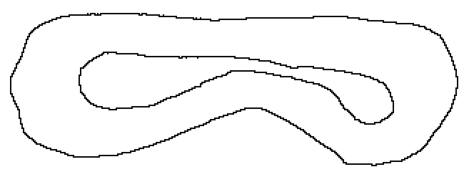
\includegraphics[interpolate=true,width=4.640000in,height=1.720000in]{contents/chapt6/figs/steer/circle_path-img0.png}}%
\end{pgfscope}%
\begin{pgfscope}%
\pgfpathrectangle{\pgfqpoint{0.180000in}{0.568773in}}{\pgfqpoint{4.640000in}{1.862455in}}%
\pgfusepath{clip}%
\pgfsetbuttcap%
\pgfsetroundjoin%
\pgfsetlinewidth{1.505625pt}%
\definecolor{currentstroke}{rgb}{0.501961,0.501961,0.501961}%
\pgfsetstrokecolor{currentstroke}%
\pgfsetdash{{5.550000pt}{2.400000pt}}{0.000000pt}%
\pgfpathmoveto{\pgfqpoint{2.748599in}{1.536334in}}%
\pgfpathlineto{\pgfqpoint{2.859178in}{1.507822in}}%
\pgfpathlineto{\pgfqpoint{3.025961in}{1.468532in}}%
\pgfpathlineto{\pgfqpoint{3.080058in}{1.450851in}}%
\pgfpathlineto{\pgfqpoint{3.133508in}{1.430578in}}%
\pgfpathlineto{\pgfqpoint{3.213425in}{1.397804in}}%
\pgfpathlineto{\pgfqpoint{3.239320in}{1.385500in}}%
\pgfpathlineto{\pgfqpoint{3.264276in}{1.371777in}}%
\pgfpathlineto{\pgfqpoint{3.287949in}{1.356186in}}%
\pgfpathlineto{\pgfqpoint{3.310161in}{1.338509in}}%
\pgfpathlineto{\pgfqpoint{3.373726in}{1.280770in}}%
\pgfpathlineto{\pgfqpoint{3.396127in}{1.263017in}}%
\pgfpathlineto{\pgfqpoint{3.420010in}{1.247223in}}%
\pgfpathlineto{\pgfqpoint{3.494075in}{1.203552in}}%
\pgfpathlineto{\pgfqpoint{3.516924in}{1.186917in}}%
\pgfpathlineto{\pgfqpoint{3.537800in}{1.167904in}}%
\pgfpathlineto{\pgfqpoint{3.576119in}{1.125509in}}%
\pgfpathlineto{\pgfqpoint{3.595206in}{1.103988in}}%
\pgfpathlineto{\pgfqpoint{3.615342in}{1.083491in}}%
\pgfpathlineto{\pgfqpoint{3.637175in}{1.064810in}}%
\pgfpathlineto{\pgfqpoint{3.660647in}{1.048174in}}%
\pgfpathlineto{\pgfqpoint{3.685528in}{1.033672in}}%
\pgfpathlineto{\pgfqpoint{3.711586in}{1.021393in}}%
\pgfpathlineto{\pgfqpoint{3.738589in}{1.011426in}}%
\pgfpathlineto{\pgfqpoint{3.766311in}{1.003825in}}%
\pgfpathlineto{\pgfqpoint{3.794550in}{0.998500in}}%
\pgfpathlineto{\pgfqpoint{3.823109in}{0.995327in}}%
\pgfpathlineto{\pgfqpoint{3.851792in}{0.994182in}}%
\pgfpathlineto{\pgfqpoint{3.880403in}{0.994939in}}%
\pgfpathlineto{\pgfqpoint{3.908790in}{0.997437in}}%
\pgfpathlineto{\pgfqpoint{3.965073in}{1.006414in}}%
\pgfpathlineto{\pgfqpoint{4.049383in}{1.024894in}}%
\pgfpathlineto{\pgfqpoint{4.077352in}{1.031984in}}%
\pgfpathlineto{\pgfqpoint{4.104821in}{1.040258in}}%
\pgfpathlineto{\pgfqpoint{4.131477in}{1.050265in}}%
\pgfpathlineto{\pgfqpoint{4.157006in}{1.062556in}}%
\pgfpathlineto{\pgfqpoint{4.181152in}{1.077519in}}%
\pgfpathlineto{\pgfqpoint{4.203873in}{1.094904in}}%
\pgfpathlineto{\pgfqpoint{4.225184in}{1.114303in}}%
\pgfpathlineto{\pgfqpoint{4.245098in}{1.135305in}}%
\pgfpathlineto{\pgfqpoint{4.263629in}{1.157501in}}%
\pgfpathlineto{\pgfqpoint{4.280822in}{1.180531in}}%
\pgfpathlineto{\pgfqpoint{4.296836in}{1.204235in}}%
\pgfpathlineto{\pgfqpoint{4.326099in}{1.253228in}}%
\pgfpathlineto{\pgfqpoint{4.352881in}{1.303635in}}%
\pgfpathlineto{\pgfqpoint{4.377091in}{1.355358in}}%
\pgfpathlineto{\pgfqpoint{4.387720in}{1.381912in}}%
\pgfpathlineto{\pgfqpoint{4.397080in}{1.409041in}}%
\pgfpathlineto{\pgfqpoint{4.404944in}{1.436785in}}%
\pgfpathlineto{\pgfqpoint{4.411042in}{1.464999in}}%
\pgfpathlineto{\pgfqpoint{4.415090in}{1.493493in}}%
\pgfpathlineto{\pgfqpoint{4.416807in}{1.522078in}}%
\pgfpathlineto{\pgfqpoint{4.415910in}{1.550563in}}%
\pgfpathlineto{\pgfqpoint{4.412228in}{1.578783in}}%
\pgfpathlineto{\pgfqpoint{4.406038in}{1.606662in}}%
\pgfpathlineto{\pgfqpoint{4.397729in}{1.634147in}}%
\pgfpathlineto{\pgfqpoint{4.387688in}{1.661187in}}%
\pgfpathlineto{\pgfqpoint{4.376305in}{1.687729in}}%
\pgfpathlineto{\pgfqpoint{4.363867in}{1.713701in}}%
\pgfpathlineto{\pgfqpoint{4.350256in}{1.738944in}}%
\pgfpathlineto{\pgfqpoint{4.335255in}{1.763281in}}%
\pgfpathlineto{\pgfqpoint{4.318644in}{1.786534in}}%
\pgfpathlineto{\pgfqpoint{4.300205in}{1.808526in}}%
\pgfpathlineto{\pgfqpoint{4.279792in}{1.829039in}}%
\pgfpathlineto{\pgfqpoint{4.257549in}{1.847707in}}%
\pgfpathlineto{\pgfqpoint{4.233690in}{1.864124in}}%
\pgfpathlineto{\pgfqpoint{4.208432in}{1.877883in}}%
\pgfpathlineto{\pgfqpoint{4.181991in}{1.888579in}}%
\pgfpathlineto{\pgfqpoint{4.154597in}{1.896066in}}%
\pgfpathlineto{\pgfqpoint{4.126547in}{1.901238in}}%
\pgfpathlineto{\pgfqpoint{4.069724in}{1.909252in}}%
\pgfpathlineto{\pgfqpoint{4.041576in}{1.914403in}}%
\pgfpathlineto{\pgfqpoint{4.013932in}{1.921522in}}%
\pgfpathlineto{\pgfqpoint{3.905084in}{1.956270in}}%
\pgfpathlineto{\pgfqpoint{3.877311in}{1.962551in}}%
\pgfpathlineto{\pgfqpoint{3.820845in}{1.971182in}}%
\pgfpathlineto{\pgfqpoint{3.678882in}{1.987948in}}%
\pgfpathlineto{\pgfqpoint{3.509014in}{2.011489in}}%
\pgfpathlineto{\pgfqpoint{3.480556in}{2.012755in}}%
\pgfpathlineto{\pgfqpoint{3.423496in}{2.010893in}}%
\pgfpathlineto{\pgfqpoint{3.366383in}{2.007935in}}%
\pgfpathlineto{\pgfqpoint{3.337865in}{2.008035in}}%
\pgfpathlineto{\pgfqpoint{3.309397in}{2.009957in}}%
\pgfpathlineto{\pgfqpoint{3.224080in}{2.018927in}}%
\pgfpathlineto{\pgfqpoint{3.195584in}{2.019825in}}%
\pgfpathlineto{\pgfqpoint{3.167028in}{2.018451in}}%
\pgfpathlineto{\pgfqpoint{3.081450in}{2.010421in}}%
\pgfpathlineto{\pgfqpoint{3.053127in}{2.010389in}}%
\pgfpathlineto{\pgfqpoint{3.024969in}{2.013276in}}%
\pgfpathlineto{\pgfqpoint{2.996925in}{2.018381in}}%
\pgfpathlineto{\pgfqpoint{2.912712in}{2.036213in}}%
\pgfpathlineto{\pgfqpoint{2.884384in}{2.039651in}}%
\pgfpathlineto{\pgfqpoint{2.855910in}{2.041417in}}%
\pgfpathlineto{\pgfqpoint{2.798686in}{2.041633in}}%
\pgfpathlineto{\pgfqpoint{2.712756in}{2.039850in}}%
\pgfpathlineto{\pgfqpoint{2.655691in}{2.041101in}}%
\pgfpathlineto{\pgfqpoint{2.627271in}{2.043294in}}%
\pgfpathlineto{\pgfqpoint{2.570658in}{2.050992in}}%
\pgfpathlineto{\pgfqpoint{2.514104in}{2.059309in}}%
\pgfpathlineto{\pgfqpoint{2.485749in}{2.062124in}}%
\pgfpathlineto{\pgfqpoint{2.457301in}{2.063382in}}%
\pgfpathlineto{\pgfqpoint{2.400196in}{2.062433in}}%
\pgfpathlineto{\pgfqpoint{2.285884in}{2.057999in}}%
\pgfpathlineto{\pgfqpoint{2.200309in}{2.055043in}}%
\pgfpathlineto{\pgfqpoint{2.086211in}{2.048222in}}%
\pgfpathlineto{\pgfqpoint{2.057715in}{2.047964in}}%
\pgfpathlineto{\pgfqpoint{2.000771in}{2.050799in}}%
\pgfpathlineto{\pgfqpoint{1.915258in}{2.057400in}}%
\pgfpathlineto{\pgfqpoint{1.801032in}{2.061842in}}%
\pgfpathlineto{\pgfqpoint{1.772664in}{2.064479in}}%
\pgfpathlineto{\pgfqpoint{1.716313in}{2.073550in}}%
\pgfpathlineto{\pgfqpoint{1.660080in}{2.083914in}}%
\pgfpathlineto{\pgfqpoint{1.631842in}{2.087978in}}%
\pgfpathlineto{\pgfqpoint{1.603454in}{2.090592in}}%
\pgfpathlineto{\pgfqpoint{1.546347in}{2.092078in}}%
\pgfpathlineto{\pgfqpoint{1.489093in}{2.090338in}}%
\pgfpathlineto{\pgfqpoint{1.403425in}{2.087301in}}%
\pgfpathlineto{\pgfqpoint{1.374885in}{2.087991in}}%
\pgfpathlineto{\pgfqpoint{1.346323in}{2.090338in}}%
\pgfpathlineto{\pgfqpoint{1.289184in}{2.099567in}}%
\pgfpathlineto{\pgfqpoint{1.260745in}{2.104158in}}%
\pgfpathlineto{\pgfqpoint{1.232494in}{2.107009in}}%
\pgfpathlineto{\pgfqpoint{1.204509in}{2.106826in}}%
\pgfpathlineto{\pgfqpoint{1.176841in}{2.102715in}}%
\pgfpathlineto{\pgfqpoint{1.149436in}{2.095374in}}%
\pgfpathlineto{\pgfqpoint{1.095103in}{2.075398in}}%
\pgfpathlineto{\pgfqpoint{1.040896in}{2.055432in}}%
\pgfpathlineto{\pgfqpoint{0.905167in}{2.011059in}}%
\pgfpathlineto{\pgfqpoint{0.878494in}{2.000102in}}%
\pgfpathlineto{\pgfqpoint{0.852582in}{1.987660in}}%
\pgfpathlineto{\pgfqpoint{0.827794in}{1.973422in}}%
\pgfpathlineto{\pgfqpoint{0.804495in}{1.957079in}}%
\pgfpathlineto{\pgfqpoint{0.782969in}{1.938436in}}%
\pgfpathlineto{\pgfqpoint{0.763183in}{1.917761in}}%
\pgfpathlineto{\pgfqpoint{0.745022in}{1.895437in}}%
\pgfpathlineto{\pgfqpoint{0.728375in}{1.871847in}}%
\pgfpathlineto{\pgfqpoint{0.713128in}{1.847375in}}%
\pgfpathlineto{\pgfqpoint{0.699181in}{1.822334in}}%
\pgfpathlineto{\pgfqpoint{0.686498in}{1.796767in}}%
\pgfpathlineto{\pgfqpoint{0.675052in}{1.770645in}}%
\pgfpathlineto{\pgfqpoint{0.664820in}{1.743942in}}%
\pgfpathlineto{\pgfqpoint{0.655778in}{1.716631in}}%
\pgfpathlineto{\pgfqpoint{0.647976in}{1.688724in}}%
\pgfpathlineto{\pgfqpoint{0.641766in}{1.660400in}}%
\pgfpathlineto{\pgfqpoint{0.637573in}{1.631878in}}%
\pgfpathlineto{\pgfqpoint{0.635825in}{1.603374in}}%
\pgfpathlineto{\pgfqpoint{0.636948in}{1.575109in}}%
\pgfpathlineto{\pgfqpoint{0.641175in}{1.547243in}}%
\pgfpathlineto{\pgfqpoint{0.647974in}{1.519713in}}%
\pgfpathlineto{\pgfqpoint{0.666388in}{1.465183in}}%
\pgfpathlineto{\pgfqpoint{0.696971in}{1.383613in}}%
\pgfpathlineto{\pgfqpoint{0.708247in}{1.357250in}}%
\pgfpathlineto{\pgfqpoint{0.721068in}{1.331965in}}%
\pgfpathlineto{\pgfqpoint{0.736056in}{1.308164in}}%
\pgfpathlineto{\pgfqpoint{0.753654in}{1.286156in}}%
\pgfpathlineto{\pgfqpoint{0.773580in}{1.265848in}}%
\pgfpathlineto{\pgfqpoint{0.795368in}{1.247050in}}%
\pgfpathlineto{\pgfqpoint{0.818556in}{1.229570in}}%
\pgfpathlineto{\pgfqpoint{0.842679in}{1.213219in}}%
\pgfpathlineto{\pgfqpoint{0.867356in}{1.197884in}}%
\pgfpathlineto{\pgfqpoint{0.892538in}{1.183770in}}%
\pgfpathlineto{\pgfqpoint{0.918259in}{1.171159in}}%
\pgfpathlineto{\pgfqpoint{0.944553in}{1.160334in}}%
\pgfpathlineto{\pgfqpoint{0.971456in}{1.151578in}}%
\pgfpathlineto{\pgfqpoint{0.998968in}{1.145010in}}%
\pgfpathlineto{\pgfqpoint{1.055286in}{1.136094in}}%
\pgfpathlineto{\pgfqpoint{1.112278in}{1.128079in}}%
\pgfpathlineto{\pgfqpoint{1.225305in}{1.108525in}}%
\pgfpathlineto{\pgfqpoint{1.253469in}{1.106912in}}%
\pgfpathlineto{\pgfqpoint{1.281664in}{1.108002in}}%
\pgfpathlineto{\pgfqpoint{1.309904in}{1.111250in}}%
\pgfpathlineto{\pgfqpoint{1.423487in}{1.129663in}}%
\pgfpathlineto{\pgfqpoint{1.480305in}{1.136693in}}%
\pgfpathlineto{\pgfqpoint{1.508414in}{1.141083in}}%
\pgfpathlineto{\pgfqpoint{1.536182in}{1.146909in}}%
\pgfpathlineto{\pgfqpoint{1.563556in}{1.154562in}}%
\pgfpathlineto{\pgfqpoint{1.645041in}{1.181398in}}%
\pgfpathlineto{\pgfqpoint{1.672675in}{1.188776in}}%
\pgfpathlineto{\pgfqpoint{1.700801in}{1.194256in}}%
\pgfpathlineto{\pgfqpoint{1.785648in}{1.207694in}}%
\pgfpathlineto{\pgfqpoint{1.813089in}{1.214600in}}%
\pgfpathlineto{\pgfqpoint{1.839693in}{1.224152in}}%
\pgfpathlineto{\pgfqpoint{1.865572in}{1.235968in}}%
\pgfpathlineto{\pgfqpoint{1.915944in}{1.263736in}}%
\pgfpathlineto{\pgfqpoint{1.990809in}{1.306541in}}%
\pgfpathlineto{\pgfqpoint{2.041609in}{1.332403in}}%
\pgfpathlineto{\pgfqpoint{2.093776in}{1.355241in}}%
\pgfpathlineto{\pgfqpoint{2.147162in}{1.375550in}}%
\pgfpathlineto{\pgfqpoint{2.254332in}{1.415185in}}%
\pgfpathlineto{\pgfqpoint{2.307234in}{1.436662in}}%
\pgfpathlineto{\pgfqpoint{2.438424in}{1.493729in}}%
\pgfpathlineto{\pgfqpoint{2.465168in}{1.503200in}}%
\pgfpathlineto{\pgfqpoint{2.492313in}{1.511143in}}%
\pgfpathlineto{\pgfqpoint{2.519842in}{1.517624in}}%
\pgfpathlineto{\pgfqpoint{2.547712in}{1.522805in}}%
\pgfpathlineto{\pgfqpoint{2.604307in}{1.529918in}}%
\pgfpathlineto{\pgfqpoint{2.661755in}{1.533784in}}%
\pgfpathlineto{\pgfqpoint{2.719714in}{1.535702in}}%
\pgfpathlineto{\pgfqpoint{2.719714in}{1.535702in}}%
\pgfusepath{stroke}%
\end{pgfscope}%
\begin{pgfscope}%
\pgfpathrectangle{\pgfqpoint{0.180000in}{0.568773in}}{\pgfqpoint{4.640000in}{1.862455in}}%
\pgfusepath{clip}%
\pgfsetbuttcap%
\pgfsetroundjoin%
\pgfsetlinewidth{1.505625pt}%
\definecolor{currentstroke}{rgb}{1.000000,0.000000,0.000000}%
\pgfsetstrokecolor{currentstroke}%
\pgfsetstrokeopacity{0.500000}%
\pgfsetdash{{9.600000pt}{2.400000pt}{1.500000pt}{2.400000pt}}{0.000000pt}%
\pgfpathmoveto{\pgfqpoint{2.978278in}{2.003226in}}%
\pgfpathlineto{\pgfqpoint{2.949724in}{2.003379in}}%
\pgfpathlineto{\pgfqpoint{2.921171in}{2.003533in}}%
\pgfpathlineto{\pgfqpoint{2.892617in}{2.003686in}}%
\pgfpathlineto{\pgfqpoint{2.864064in}{2.003839in}}%
\pgfpathlineto{\pgfqpoint{2.835511in}{2.003992in}}%
\pgfpathlineto{\pgfqpoint{2.806957in}{2.004145in}}%
\pgfpathlineto{\pgfqpoint{2.778404in}{2.004299in}}%
\pgfpathlineto{\pgfqpoint{2.749850in}{2.004452in}}%
\pgfpathlineto{\pgfqpoint{2.721297in}{2.004605in}}%
\pgfpathlineto{\pgfqpoint{2.692743in}{2.004758in}}%
\pgfpathlineto{\pgfqpoint{2.664190in}{2.004912in}}%
\pgfpathlineto{\pgfqpoint{2.635637in}{2.005065in}}%
\pgfpathlineto{\pgfqpoint{2.607083in}{2.005218in}}%
\pgfpathlineto{\pgfqpoint{2.578530in}{2.005371in}}%
\pgfpathlineto{\pgfqpoint{2.549976in}{2.005525in}}%
\pgfpathlineto{\pgfqpoint{2.521423in}{2.005678in}}%
\pgfpathlineto{\pgfqpoint{2.492869in}{2.005831in}}%
\pgfpathlineto{\pgfqpoint{2.464316in}{2.005984in}}%
\pgfpathlineto{\pgfqpoint{2.435762in}{2.006137in}}%
\pgfpathlineto{\pgfqpoint{2.407209in}{2.006291in}}%
\pgfpathlineto{\pgfqpoint{2.378656in}{2.006444in}}%
\pgfpathlineto{\pgfqpoint{2.350102in}{2.006597in}}%
\pgfpathlineto{\pgfqpoint{2.321549in}{2.006750in}}%
\pgfpathlineto{\pgfqpoint{2.292995in}{2.006904in}}%
\pgfpathlineto{\pgfqpoint{2.264442in}{2.007057in}}%
\pgfpathlineto{\pgfqpoint{2.235888in}{2.007210in}}%
\pgfpathlineto{\pgfqpoint{2.207335in}{2.007363in}}%
\pgfpathlineto{\pgfqpoint{2.178782in}{2.007517in}}%
\pgfpathlineto{\pgfqpoint{2.150228in}{2.007670in}}%
\pgfpathlineto{\pgfqpoint{2.121675in}{2.007823in}}%
\pgfpathlineto{\pgfqpoint{2.093121in}{2.007976in}}%
\pgfpathlineto{\pgfqpoint{2.064568in}{2.008129in}}%
\pgfpathlineto{\pgfqpoint{2.036014in}{2.008283in}}%
\pgfpathlineto{\pgfqpoint{2.007461in}{2.008436in}}%
\pgfpathlineto{\pgfqpoint{1.978908in}{2.008589in}}%
\pgfusepath{stroke}%
\end{pgfscope}%
\begin{pgfscope}%
\pgfpathrectangle{\pgfqpoint{0.180000in}{0.568773in}}{\pgfqpoint{4.640000in}{1.862455in}}%
\pgfusepath{clip}%
\pgfsetrectcap%
\pgfsetroundjoin%
\pgfsetlinewidth{1.505625pt}%
\definecolor{currentstroke}{rgb}{1.000000,0.000000,0.000000}%
\pgfsetstrokecolor{currentstroke}%
\pgfsetstrokeopacity{0.500000}%
\pgfsetdash{}{0pt}%
\pgfpathmoveto{\pgfqpoint{2.978278in}{2.003226in}}%
\pgfusepath{stroke}%
\end{pgfscope}%
\begin{pgfscope}%
\pgfpathrectangle{\pgfqpoint{0.180000in}{0.568773in}}{\pgfqpoint{4.640000in}{1.862455in}}%
\pgfusepath{clip}%
\pgfsetbuttcap%
\pgfsetmiterjoin%
\definecolor{currentfill}{rgb}{1.000000,0.000000,0.000000}%
\pgfsetfillcolor{currentfill}%
\pgfsetfillopacity{0.500000}%
\pgfsetlinewidth{1.003750pt}%
\definecolor{currentstroke}{rgb}{1.000000,0.000000,0.000000}%
\pgfsetstrokecolor{currentstroke}%
\pgfsetstrokeopacity{0.500000}%
\pgfsetdash{}{0pt}%
\pgfsys@defobject{currentmarker}{\pgfqpoint{-0.041667in}{-0.041667in}}{\pgfqpoint{0.041667in}{0.041667in}}{%
\pgfpathmoveto{\pgfqpoint{-0.041667in}{-0.041667in}}%
\pgfpathlineto{\pgfqpoint{0.041667in}{-0.041667in}}%
\pgfpathlineto{\pgfqpoint{0.041667in}{0.041667in}}%
\pgfpathlineto{\pgfqpoint{-0.041667in}{0.041667in}}%
\pgfpathlineto{\pgfqpoint{-0.041667in}{-0.041667in}}%
\pgfpathclose%
\pgfusepath{stroke,fill}%
}%
\begin{pgfscope}%
\pgfsys@transformshift{2.978278in}{2.003226in}%
\pgfsys@useobject{currentmarker}{}%
\end{pgfscope}%
\end{pgfscope}%
\begin{pgfscope}%
\pgfpathrectangle{\pgfqpoint{0.180000in}{0.568773in}}{\pgfqpoint{4.640000in}{1.862455in}}%
\pgfusepath{clip}%
\pgfsetbuttcap%
\pgfsetroundjoin%
\pgfsetlinewidth{1.505625pt}%
\definecolor{currentstroke}{rgb}{1.000000,0.000000,0.000000}%
\pgfsetstrokecolor{currentstroke}%
\pgfsetstrokeopacity{0.500000}%
\pgfsetdash{{9.600000pt}{2.400000pt}{1.500000pt}{2.400000pt}}{0.000000pt}%
\pgfpathmoveto{\pgfqpoint{2.522883in}{2.016937in}}%
\pgfpathlineto{\pgfqpoint{2.494586in}{2.020754in}}%
\pgfpathlineto{\pgfqpoint{2.466240in}{2.024197in}}%
\pgfpathlineto{\pgfqpoint{2.437852in}{2.027264in}}%
\pgfpathlineto{\pgfqpoint{2.409425in}{2.029954in}}%
\pgfpathlineto{\pgfqpoint{2.380965in}{2.032268in}}%
\pgfpathlineto{\pgfqpoint{2.352478in}{2.034204in}}%
\pgfpathlineto{\pgfqpoint{2.323966in}{2.035763in}}%
\pgfpathlineto{\pgfqpoint{2.295437in}{2.036944in}}%
\pgfpathlineto{\pgfqpoint{2.266895in}{2.037747in}}%
\pgfpathlineto{\pgfqpoint{2.238344in}{2.038172in}}%
\pgfpathlineto{\pgfqpoint{2.209791in}{2.038219in}}%
\pgfpathlineto{\pgfqpoint{2.181239in}{2.037888in}}%
\pgfpathlineto{\pgfqpoint{2.152694in}{2.037178in}}%
\pgfpathlineto{\pgfqpoint{2.124161in}{2.036090in}}%
\pgfpathlineto{\pgfqpoint{2.095645in}{2.034625in}}%
\pgfpathlineto{\pgfqpoint{2.067151in}{2.032782in}}%
\pgfpathlineto{\pgfqpoint{2.038684in}{2.030562in}}%
\pgfpathlineto{\pgfqpoint{2.010248in}{2.027965in}}%
\pgfpathlineto{\pgfqpoint{1.981850in}{2.024988in}}%
\pgfpathlineto{\pgfqpoint{1.953475in}{2.021798in}}%
\pgfpathlineto{\pgfqpoint{1.925098in}{2.018629in}}%
\pgfpathlineto{\pgfqpoint{1.896720in}{2.015461in}}%
\pgfpathlineto{\pgfqpoint{1.868344in}{2.012285in}}%
\pgfpathlineto{\pgfqpoint{1.839967in}{2.009108in}}%
\pgfpathlineto{\pgfqpoint{1.811590in}{2.005933in}}%
\pgfpathlineto{\pgfqpoint{1.783213in}{2.002759in}}%
\pgfpathlineto{\pgfqpoint{1.754837in}{1.999584in}}%
\pgfpathlineto{\pgfqpoint{1.726460in}{1.996409in}}%
\pgfpathlineto{\pgfqpoint{1.698083in}{1.993234in}}%
\pgfpathlineto{\pgfqpoint{1.669706in}{1.990059in}}%
\pgfpathlineto{\pgfqpoint{1.641329in}{1.986884in}}%
\pgfpathlineto{\pgfqpoint{1.612953in}{1.983709in}}%
\pgfpathlineto{\pgfqpoint{1.584576in}{1.980534in}}%
\pgfpathlineto{\pgfqpoint{1.556199in}{1.977359in}}%
\pgfpathlineto{\pgfqpoint{1.527822in}{1.974184in}}%
\pgfpathlineto{\pgfqpoint{1.499446in}{1.971010in}}%
\pgfpathlineto{\pgfqpoint{1.471069in}{1.967835in}}%
\pgfusepath{stroke}%
\end{pgfscope}%
\begin{pgfscope}%
\pgfpathrectangle{\pgfqpoint{0.180000in}{0.568773in}}{\pgfqpoint{4.640000in}{1.862455in}}%
\pgfusepath{clip}%
\pgfsetrectcap%
\pgfsetroundjoin%
\pgfsetlinewidth{1.505625pt}%
\definecolor{currentstroke}{rgb}{1.000000,0.000000,0.000000}%
\pgfsetstrokecolor{currentstroke}%
\pgfsetstrokeopacity{0.500000}%
\pgfsetdash{}{0pt}%
\pgfpathmoveto{\pgfqpoint{2.522883in}{2.016937in}}%
\pgfusepath{stroke}%
\end{pgfscope}%
\begin{pgfscope}%
\pgfpathrectangle{\pgfqpoint{0.180000in}{0.568773in}}{\pgfqpoint{4.640000in}{1.862455in}}%
\pgfusepath{clip}%
\pgfsetbuttcap%
\pgfsetmiterjoin%
\definecolor{currentfill}{rgb}{1.000000,0.000000,0.000000}%
\pgfsetfillcolor{currentfill}%
\pgfsetfillopacity{0.500000}%
\pgfsetlinewidth{1.003750pt}%
\definecolor{currentstroke}{rgb}{1.000000,0.000000,0.000000}%
\pgfsetstrokecolor{currentstroke}%
\pgfsetstrokeopacity{0.500000}%
\pgfsetdash{}{0pt}%
\pgfsys@defobject{currentmarker}{\pgfqpoint{-0.041667in}{-0.041667in}}{\pgfqpoint{0.041667in}{0.041667in}}{%
\pgfpathmoveto{\pgfqpoint{-0.041667in}{-0.041667in}}%
\pgfpathlineto{\pgfqpoint{0.041667in}{-0.041667in}}%
\pgfpathlineto{\pgfqpoint{0.041667in}{0.041667in}}%
\pgfpathlineto{\pgfqpoint{-0.041667in}{0.041667in}}%
\pgfpathlineto{\pgfqpoint{-0.041667in}{-0.041667in}}%
\pgfpathclose%
\pgfusepath{stroke,fill}%
}%
\begin{pgfscope}%
\pgfsys@transformshift{2.522883in}{2.016937in}%
\pgfsys@useobject{currentmarker}{}%
\end{pgfscope}%
\end{pgfscope}%
\begin{pgfscope}%
\pgfpathrectangle{\pgfqpoint{0.180000in}{0.568773in}}{\pgfqpoint{4.640000in}{1.862455in}}%
\pgfusepath{clip}%
\pgfsetbuttcap%
\pgfsetroundjoin%
\pgfsetlinewidth{1.505625pt}%
\definecolor{currentstroke}{rgb}{1.000000,0.000000,0.000000}%
\pgfsetstrokecolor{currentstroke}%
\pgfsetstrokeopacity{0.500000}%
\pgfsetdash{{9.600000pt}{2.400000pt}{1.500000pt}{2.400000pt}}{0.000000pt}%
\pgfpathmoveto{\pgfqpoint{1.953956in}{2.073469in}}%
\pgfpathlineto{\pgfqpoint{1.925629in}{2.077058in}}%
\pgfpathlineto{\pgfqpoint{1.897282in}{2.080490in}}%
\pgfpathlineto{\pgfqpoint{1.868917in}{2.083767in}}%
\pgfpathlineto{\pgfqpoint{1.840534in}{2.086886in}}%
\pgfpathlineto{\pgfqpoint{1.812134in}{2.089850in}}%
\pgfpathlineto{\pgfqpoint{1.783719in}{2.092656in}}%
\pgfpathlineto{\pgfqpoint{1.755288in}{2.095306in}}%
\pgfpathlineto{\pgfqpoint{1.726843in}{2.097800in}}%
\pgfpathlineto{\pgfqpoint{1.698385in}{2.100136in}}%
\pgfpathlineto{\pgfqpoint{1.669915in}{2.102316in}}%
\pgfpathlineto{\pgfqpoint{1.641433in}{2.104338in}}%
\pgfpathlineto{\pgfqpoint{1.612940in}{2.106204in}}%
\pgfpathlineto{\pgfqpoint{1.584437in}{2.107912in}}%
\pgfpathlineto{\pgfqpoint{1.555926in}{2.109463in}}%
\pgfpathlineto{\pgfqpoint{1.527406in}{2.110857in}}%
\pgfpathlineto{\pgfqpoint{1.498879in}{2.112094in}}%
\pgfpathlineto{\pgfqpoint{1.470345in}{2.113173in}}%
\pgfpathlineto{\pgfqpoint{1.441806in}{2.114095in}}%
\pgfpathlineto{\pgfqpoint{1.413263in}{2.114859in}}%
\pgfpathlineto{\pgfqpoint{1.384717in}{2.115540in}}%
\pgfpathlineto{\pgfqpoint{1.356172in}{2.116231in}}%
\pgfpathlineto{\pgfqpoint{1.327626in}{2.116921in}}%
\pgfpathlineto{\pgfqpoint{1.299081in}{2.117609in}}%
\pgfpathlineto{\pgfqpoint{1.270535in}{2.118296in}}%
\pgfpathlineto{\pgfqpoint{1.241989in}{2.118983in}}%
\pgfpathlineto{\pgfqpoint{1.213444in}{2.119671in}}%
\pgfpathlineto{\pgfqpoint{1.184898in}{2.120359in}}%
\pgfpathlineto{\pgfqpoint{1.156353in}{2.121047in}}%
\pgfpathlineto{\pgfqpoint{1.127807in}{2.121735in}}%
\pgfpathlineto{\pgfqpoint{1.099262in}{2.122423in}}%
\pgfpathlineto{\pgfqpoint{1.070716in}{2.123110in}}%
\pgfpathlineto{\pgfqpoint{1.042170in}{2.123798in}}%
\pgfpathlineto{\pgfqpoint{1.013625in}{2.124486in}}%
\pgfpathlineto{\pgfqpoint{0.985079in}{2.125174in}}%
\pgfpathlineto{\pgfqpoint{0.956534in}{2.125862in}}%
\pgfpathlineto{\pgfqpoint{0.927988in}{2.126549in}}%
\pgfusepath{stroke}%
\end{pgfscope}%
\begin{pgfscope}%
\pgfpathrectangle{\pgfqpoint{0.180000in}{0.568773in}}{\pgfqpoint{4.640000in}{1.862455in}}%
\pgfusepath{clip}%
\pgfsetrectcap%
\pgfsetroundjoin%
\pgfsetlinewidth{1.505625pt}%
\definecolor{currentstroke}{rgb}{1.000000,0.000000,0.000000}%
\pgfsetstrokecolor{currentstroke}%
\pgfsetstrokeopacity{0.500000}%
\pgfsetdash{}{0pt}%
\pgfpathmoveto{\pgfqpoint{1.953956in}{2.073469in}}%
\pgfusepath{stroke}%
\end{pgfscope}%
\begin{pgfscope}%
\pgfpathrectangle{\pgfqpoint{0.180000in}{0.568773in}}{\pgfqpoint{4.640000in}{1.862455in}}%
\pgfusepath{clip}%
\pgfsetbuttcap%
\pgfsetmiterjoin%
\definecolor{currentfill}{rgb}{1.000000,0.000000,0.000000}%
\pgfsetfillcolor{currentfill}%
\pgfsetfillopacity{0.500000}%
\pgfsetlinewidth{1.003750pt}%
\definecolor{currentstroke}{rgb}{1.000000,0.000000,0.000000}%
\pgfsetstrokecolor{currentstroke}%
\pgfsetstrokeopacity{0.500000}%
\pgfsetdash{}{0pt}%
\pgfsys@defobject{currentmarker}{\pgfqpoint{-0.041667in}{-0.041667in}}{\pgfqpoint{0.041667in}{0.041667in}}{%
\pgfpathmoveto{\pgfqpoint{-0.041667in}{-0.041667in}}%
\pgfpathlineto{\pgfqpoint{0.041667in}{-0.041667in}}%
\pgfpathlineto{\pgfqpoint{0.041667in}{0.041667in}}%
\pgfpathlineto{\pgfqpoint{-0.041667in}{0.041667in}}%
\pgfpathlineto{\pgfqpoint{-0.041667in}{-0.041667in}}%
\pgfpathclose%
\pgfusepath{stroke,fill}%
}%
\begin{pgfscope}%
\pgfsys@transformshift{1.953956in}{2.073469in}%
\pgfsys@useobject{currentmarker}{}%
\end{pgfscope}%
\end{pgfscope}%
\begin{pgfscope}%
\pgfpathrectangle{\pgfqpoint{0.180000in}{0.568773in}}{\pgfqpoint{4.640000in}{1.862455in}}%
\pgfusepath{clip}%
\pgfsetbuttcap%
\pgfsetroundjoin%
\pgfsetlinewidth{1.505625pt}%
\definecolor{currentstroke}{rgb}{1.000000,0.000000,0.000000}%
\pgfsetstrokecolor{currentstroke}%
\pgfsetstrokeopacity{0.500000}%
\pgfsetdash{{9.600000pt}{2.400000pt}{1.500000pt}{2.400000pt}}{0.000000pt}%
\pgfpathmoveto{\pgfqpoint{1.383208in}{2.120486in}}%
\pgfpathlineto{\pgfqpoint{1.354911in}{2.116701in}}%
\pgfpathlineto{\pgfqpoint{1.326964in}{2.110869in}}%
\pgfpathlineto{\pgfqpoint{1.299516in}{2.103018in}}%
\pgfpathlineto{\pgfqpoint{1.272712in}{2.093191in}}%
\pgfpathlineto{\pgfqpoint{1.246694in}{2.081439in}}%
\pgfpathlineto{\pgfqpoint{1.221600in}{2.067826in}}%
\pgfpathlineto{\pgfqpoint{1.197563in}{2.052423in}}%
\pgfpathlineto{\pgfqpoint{1.174710in}{2.035312in}}%
\pgfpathlineto{\pgfqpoint{1.153163in}{2.016584in}}%
\pgfpathlineto{\pgfqpoint{1.133035in}{1.996337in}}%
\pgfpathlineto{\pgfqpoint{1.114434in}{1.974680in}}%
\pgfpathlineto{\pgfqpoint{1.097458in}{1.951727in}}%
\pgfpathlineto{\pgfqpoint{1.082197in}{1.927600in}}%
\pgfpathlineto{\pgfqpoint{1.068731in}{1.902426in}}%
\pgfpathlineto{\pgfqpoint{1.057134in}{1.876339in}}%
\pgfpathlineto{\pgfqpoint{1.047464in}{1.849477in}}%
\pgfpathlineto{\pgfqpoint{1.039775in}{1.821983in}}%
\pgfpathlineto{\pgfqpoint{1.034107in}{1.794003in}}%
\pgfpathlineto{\pgfqpoint{1.030489in}{1.765684in}}%
\pgfpathlineto{\pgfqpoint{1.028941in}{1.737177in}}%
\pgfpathlineto{\pgfqpoint{1.029470in}{1.708633in}}%
\pgfpathlineto{\pgfqpoint{1.031618in}{1.680160in}}%
\pgfpathlineto{\pgfqpoint{1.033710in}{1.651683in}}%
\pgfpathlineto{\pgfqpoint{1.035766in}{1.623204in}}%
\pgfpathlineto{\pgfqpoint{1.037869in}{1.594727in}}%
\pgfpathlineto{\pgfqpoint{1.039991in}{1.566252in}}%
\pgfpathlineto{\pgfqpoint{1.042101in}{1.537776in}}%
\pgfpathlineto{\pgfqpoint{1.044204in}{1.509300in}}%
\pgfpathlineto{\pgfqpoint{1.046309in}{1.480824in}}%
\pgfpathlineto{\pgfqpoint{1.048416in}{1.452348in}}%
\pgfpathlineto{\pgfqpoint{1.050523in}{1.423872in}}%
\pgfpathlineto{\pgfqpoint{1.052630in}{1.395396in}}%
\pgfpathlineto{\pgfqpoint{1.054736in}{1.366920in}}%
\pgfpathlineto{\pgfqpoint{1.056843in}{1.338444in}}%
\pgfpathlineto{\pgfqpoint{1.058949in}{1.309968in}}%
\pgfpathlineto{\pgfqpoint{1.061056in}{1.281492in}}%
\pgfpathlineto{\pgfqpoint{1.063163in}{1.253016in}}%
\pgfpathlineto{\pgfqpoint{1.065269in}{1.224540in}}%
\pgfpathlineto{\pgfqpoint{1.067376in}{1.196064in}}%
\pgfusepath{stroke}%
\end{pgfscope}%
\begin{pgfscope}%
\pgfpathrectangle{\pgfqpoint{0.180000in}{0.568773in}}{\pgfqpoint{4.640000in}{1.862455in}}%
\pgfusepath{clip}%
\pgfsetrectcap%
\pgfsetroundjoin%
\pgfsetlinewidth{1.505625pt}%
\definecolor{currentstroke}{rgb}{1.000000,0.000000,0.000000}%
\pgfsetstrokecolor{currentstroke}%
\pgfsetstrokeopacity{0.500000}%
\pgfsetdash{}{0pt}%
\pgfpathmoveto{\pgfqpoint{1.383208in}{2.120486in}}%
\pgfusepath{stroke}%
\end{pgfscope}%
\begin{pgfscope}%
\pgfpathrectangle{\pgfqpoint{0.180000in}{0.568773in}}{\pgfqpoint{4.640000in}{1.862455in}}%
\pgfusepath{clip}%
\pgfsetbuttcap%
\pgfsetmiterjoin%
\definecolor{currentfill}{rgb}{1.000000,0.000000,0.000000}%
\pgfsetfillcolor{currentfill}%
\pgfsetfillopacity{0.500000}%
\pgfsetlinewidth{1.003750pt}%
\definecolor{currentstroke}{rgb}{1.000000,0.000000,0.000000}%
\pgfsetstrokecolor{currentstroke}%
\pgfsetstrokeopacity{0.500000}%
\pgfsetdash{}{0pt}%
\pgfsys@defobject{currentmarker}{\pgfqpoint{-0.041667in}{-0.041667in}}{\pgfqpoint{0.041667in}{0.041667in}}{%
\pgfpathmoveto{\pgfqpoint{-0.041667in}{-0.041667in}}%
\pgfpathlineto{\pgfqpoint{0.041667in}{-0.041667in}}%
\pgfpathlineto{\pgfqpoint{0.041667in}{0.041667in}}%
\pgfpathlineto{\pgfqpoint{-0.041667in}{0.041667in}}%
\pgfpathlineto{\pgfqpoint{-0.041667in}{-0.041667in}}%
\pgfpathclose%
\pgfusepath{stroke,fill}%
}%
\begin{pgfscope}%
\pgfsys@transformshift{1.383208in}{2.120486in}%
\pgfsys@useobject{currentmarker}{}%
\end{pgfscope}%
\end{pgfscope}%
\begin{pgfscope}%
\pgfpathrectangle{\pgfqpoint{0.180000in}{0.568773in}}{\pgfqpoint{4.640000in}{1.862455in}}%
\pgfusepath{clip}%
\pgfsetbuttcap%
\pgfsetroundjoin%
\pgfsetlinewidth{1.505625pt}%
\definecolor{currentstroke}{rgb}{1.000000,0.000000,0.000000}%
\pgfsetstrokecolor{currentstroke}%
\pgfsetstrokeopacity{0.500000}%
\pgfsetdash{{9.600000pt}{2.400000pt}{1.500000pt}{2.400000pt}}{0.000000pt}%
\pgfpathmoveto{\pgfqpoint{0.907255in}{1.872500in}}%
\pgfpathlineto{\pgfqpoint{0.902008in}{1.844436in}}%
\pgfpathlineto{\pgfqpoint{0.898557in}{1.816096in}}%
\pgfpathlineto{\pgfqpoint{0.896917in}{1.787593in}}%
\pgfpathlineto{\pgfqpoint{0.897094in}{1.759043in}}%
\pgfpathlineto{\pgfqpoint{0.899087in}{1.730563in}}%
\pgfpathlineto{\pgfqpoint{0.902890in}{1.702267in}}%
\pgfpathlineto{\pgfqpoint{0.908485in}{1.674271in}}%
\pgfpathlineto{\pgfqpoint{0.915851in}{1.646688in}}%
\pgfpathlineto{\pgfqpoint{0.924957in}{1.619629in}}%
\pgfpathlineto{\pgfqpoint{0.935767in}{1.593204in}}%
\pgfpathlineto{\pgfqpoint{0.948236in}{1.567522in}}%
\pgfpathlineto{\pgfqpoint{0.962315in}{1.542684in}}%
\pgfpathlineto{\pgfqpoint{0.977946in}{1.518793in}}%
\pgfpathlineto{\pgfqpoint{0.995066in}{1.495946in}}%
\pgfpathlineto{\pgfqpoint{1.013605in}{1.474234in}}%
\pgfpathlineto{\pgfqpoint{1.033488in}{1.453746in}}%
\pgfpathlineto{\pgfqpoint{1.054635in}{1.434565in}}%
\pgfpathlineto{\pgfqpoint{1.076959in}{1.416769in}}%
\pgfpathlineto{\pgfqpoint{1.100371in}{1.400429in}}%
\pgfpathlineto{\pgfqpoint{1.124775in}{1.385611in}}%
\pgfpathlineto{\pgfqpoint{1.150031in}{1.372294in}}%
\pgfpathlineto{\pgfqpoint{1.175406in}{1.359200in}}%
\pgfpathlineto{\pgfqpoint{1.200748in}{1.346044in}}%
\pgfpathlineto{\pgfqpoint{1.226105in}{1.332917in}}%
\pgfpathlineto{\pgfqpoint{1.251475in}{1.319813in}}%
\pgfpathlineto{\pgfqpoint{1.276842in}{1.306704in}}%
\pgfpathlineto{\pgfqpoint{1.302205in}{1.293588in}}%
\pgfpathlineto{\pgfqpoint{1.327568in}{1.280471in}}%
\pgfpathlineto{\pgfqpoint{1.352932in}{1.267357in}}%
\pgfpathlineto{\pgfqpoint{1.378296in}{1.254244in}}%
\pgfpathlineto{\pgfqpoint{1.403660in}{1.241129in}}%
\pgfpathlineto{\pgfqpoint{1.429024in}{1.228015in}}%
\pgfpathlineto{\pgfqpoint{1.454388in}{1.214900in}}%
\pgfpathlineto{\pgfqpoint{1.479753in}{1.201786in}}%
\pgfpathlineto{\pgfqpoint{1.505117in}{1.188672in}}%
\pgfpathlineto{\pgfqpoint{1.530481in}{1.175557in}}%
\pgfpathlineto{\pgfqpoint{1.555845in}{1.162443in}}%
\pgfpathlineto{\pgfqpoint{1.581209in}{1.149329in}}%
\pgfusepath{stroke}%
\end{pgfscope}%
\begin{pgfscope}%
\pgfpathrectangle{\pgfqpoint{0.180000in}{0.568773in}}{\pgfqpoint{4.640000in}{1.862455in}}%
\pgfusepath{clip}%
\pgfsetrectcap%
\pgfsetroundjoin%
\pgfsetlinewidth{1.505625pt}%
\definecolor{currentstroke}{rgb}{1.000000,0.000000,0.000000}%
\pgfsetstrokecolor{currentstroke}%
\pgfsetstrokeopacity{0.500000}%
\pgfsetdash{}{0pt}%
\pgfpathmoveto{\pgfqpoint{0.907255in}{1.872500in}}%
\pgfusepath{stroke}%
\end{pgfscope}%
\begin{pgfscope}%
\pgfpathrectangle{\pgfqpoint{0.180000in}{0.568773in}}{\pgfqpoint{4.640000in}{1.862455in}}%
\pgfusepath{clip}%
\pgfsetbuttcap%
\pgfsetmiterjoin%
\definecolor{currentfill}{rgb}{1.000000,0.000000,0.000000}%
\pgfsetfillcolor{currentfill}%
\pgfsetfillopacity{0.500000}%
\pgfsetlinewidth{1.003750pt}%
\definecolor{currentstroke}{rgb}{1.000000,0.000000,0.000000}%
\pgfsetstrokecolor{currentstroke}%
\pgfsetstrokeopacity{0.500000}%
\pgfsetdash{}{0pt}%
\pgfsys@defobject{currentmarker}{\pgfqpoint{-0.041667in}{-0.041667in}}{\pgfqpoint{0.041667in}{0.041667in}}{%
\pgfpathmoveto{\pgfqpoint{-0.041667in}{-0.041667in}}%
\pgfpathlineto{\pgfqpoint{0.041667in}{-0.041667in}}%
\pgfpathlineto{\pgfqpoint{0.041667in}{0.041667in}}%
\pgfpathlineto{\pgfqpoint{-0.041667in}{0.041667in}}%
\pgfpathlineto{\pgfqpoint{-0.041667in}{-0.041667in}}%
\pgfpathclose%
\pgfusepath{stroke,fill}%
}%
\begin{pgfscope}%
\pgfsys@transformshift{0.907255in}{1.872500in}%
\pgfsys@useobject{currentmarker}{}%
\end{pgfscope}%
\end{pgfscope}%
\begin{pgfscope}%
\pgfpathrectangle{\pgfqpoint{0.180000in}{0.568773in}}{\pgfqpoint{4.640000in}{1.862455in}}%
\pgfusepath{clip}%
\pgfsetbuttcap%
\pgfsetroundjoin%
\pgfsetlinewidth{1.505625pt}%
\definecolor{currentstroke}{rgb}{1.000000,0.000000,0.000000}%
\pgfsetstrokecolor{currentstroke}%
\pgfsetstrokeopacity{0.500000}%
\pgfsetdash{{9.600000pt}{2.400000pt}{1.500000pt}{2.400000pt}}{0.000000pt}%
\pgfpathmoveto{\pgfqpoint{1.015369in}{1.352606in}}%
\pgfpathlineto{\pgfqpoint{1.040551in}{1.339148in}}%
\pgfpathlineto{\pgfqpoint{1.066255in}{1.326716in}}%
\pgfpathlineto{\pgfqpoint{1.092439in}{1.315331in}}%
\pgfpathlineto{\pgfqpoint{1.119061in}{1.305011in}}%
\pgfpathlineto{\pgfqpoint{1.146077in}{1.295773in}}%
\pgfpathlineto{\pgfqpoint{1.173444in}{1.287632in}}%
\pgfpathlineto{\pgfqpoint{1.201117in}{1.280601in}}%
\pgfpathlineto{\pgfqpoint{1.229051in}{1.274692in}}%
\pgfpathlineto{\pgfqpoint{1.257201in}{1.269914in}}%
\pgfpathlineto{\pgfqpoint{1.285521in}{1.266275in}}%
\pgfpathlineto{\pgfqpoint{1.313964in}{1.263781in}}%
\pgfpathlineto{\pgfqpoint{1.342484in}{1.262436in}}%
\pgfpathlineto{\pgfqpoint{1.371036in}{1.262243in}}%
\pgfpathlineto{\pgfqpoint{1.399572in}{1.263201in}}%
\pgfpathlineto{\pgfqpoint{1.428046in}{1.265308in}}%
\pgfpathlineto{\pgfqpoint{1.456413in}{1.268563in}}%
\pgfpathlineto{\pgfqpoint{1.484624in}{1.272958in}}%
\pgfpathlineto{\pgfqpoint{1.512636in}{1.278488in}}%
\pgfpathlineto{\pgfqpoint{1.540402in}{1.285141in}}%
\pgfpathlineto{\pgfqpoint{1.567900in}{1.292834in}}%
\pgfpathlineto{\pgfqpoint{1.595362in}{1.300652in}}%
\pgfpathlineto{\pgfqpoint{1.622835in}{1.308434in}}%
\pgfpathlineto{\pgfqpoint{1.650303in}{1.316235in}}%
\pgfpathlineto{\pgfqpoint{1.677766in}{1.324051in}}%
\pgfpathlineto{\pgfqpoint{1.705230in}{1.331864in}}%
\pgfpathlineto{\pgfqpoint{1.732696in}{1.339671in}}%
\pgfpathlineto{\pgfqpoint{1.760162in}{1.347479in}}%
\pgfpathlineto{\pgfqpoint{1.787627in}{1.355288in}}%
\pgfpathlineto{\pgfqpoint{1.815092in}{1.363098in}}%
\pgfpathlineto{\pgfqpoint{1.842557in}{1.370907in}}%
\pgfpathlineto{\pgfqpoint{1.870023in}{1.378716in}}%
\pgfpathlineto{\pgfqpoint{1.897488in}{1.386525in}}%
\pgfpathlineto{\pgfqpoint{1.924953in}{1.394334in}}%
\pgfpathlineto{\pgfqpoint{1.952418in}{1.402143in}}%
\pgfpathlineto{\pgfqpoint{1.979884in}{1.409952in}}%
\pgfpathlineto{\pgfqpoint{2.007349in}{1.417761in}}%
\pgfpathlineto{\pgfqpoint{2.034814in}{1.425570in}}%
\pgfusepath{stroke}%
\end{pgfscope}%
\begin{pgfscope}%
\pgfpathrectangle{\pgfqpoint{0.180000in}{0.568773in}}{\pgfqpoint{4.640000in}{1.862455in}}%
\pgfusepath{clip}%
\pgfsetrectcap%
\pgfsetroundjoin%
\pgfsetlinewidth{1.505625pt}%
\definecolor{currentstroke}{rgb}{1.000000,0.000000,0.000000}%
\pgfsetstrokecolor{currentstroke}%
\pgfsetstrokeopacity{0.500000}%
\pgfsetdash{}{0pt}%
\pgfpathmoveto{\pgfqpoint{1.015369in}{1.352606in}}%
\pgfusepath{stroke}%
\end{pgfscope}%
\begin{pgfscope}%
\pgfpathrectangle{\pgfqpoint{0.180000in}{0.568773in}}{\pgfqpoint{4.640000in}{1.862455in}}%
\pgfusepath{clip}%
\pgfsetbuttcap%
\pgfsetmiterjoin%
\definecolor{currentfill}{rgb}{1.000000,0.000000,0.000000}%
\pgfsetfillcolor{currentfill}%
\pgfsetfillopacity{0.500000}%
\pgfsetlinewidth{1.003750pt}%
\definecolor{currentstroke}{rgb}{1.000000,0.000000,0.000000}%
\pgfsetstrokecolor{currentstroke}%
\pgfsetstrokeopacity{0.500000}%
\pgfsetdash{}{0pt}%
\pgfsys@defobject{currentmarker}{\pgfqpoint{-0.041667in}{-0.041667in}}{\pgfqpoint{0.041667in}{0.041667in}}{%
\pgfpathmoveto{\pgfqpoint{-0.041667in}{-0.041667in}}%
\pgfpathlineto{\pgfqpoint{0.041667in}{-0.041667in}}%
\pgfpathlineto{\pgfqpoint{0.041667in}{0.041667in}}%
\pgfpathlineto{\pgfqpoint{-0.041667in}{0.041667in}}%
\pgfpathlineto{\pgfqpoint{-0.041667in}{-0.041667in}}%
\pgfpathclose%
\pgfusepath{stroke,fill}%
}%
\begin{pgfscope}%
\pgfsys@transformshift{1.015369in}{1.352606in}%
\pgfsys@useobject{currentmarker}{}%
\end{pgfscope}%
\end{pgfscope}%
\begin{pgfscope}%
\pgfpathrectangle{\pgfqpoint{0.180000in}{0.568773in}}{\pgfqpoint{4.640000in}{1.862455in}}%
\pgfusepath{clip}%
\pgfsetbuttcap%
\pgfsetroundjoin%
\pgfsetlinewidth{1.505625pt}%
\definecolor{currentstroke}{rgb}{1.000000,0.000000,0.000000}%
\pgfsetstrokecolor{currentstroke}%
\pgfsetstrokeopacity{0.500000}%
\pgfsetdash{{9.600000pt}{2.400000pt}{1.500000pt}{2.400000pt}}{0.000000pt}%
\pgfpathmoveto{\pgfqpoint{1.556385in}{1.214936in}}%
\pgfpathlineto{\pgfqpoint{1.584783in}{1.217901in}}%
\pgfpathlineto{\pgfqpoint{1.613057in}{1.221880in}}%
\pgfpathlineto{\pgfqpoint{1.641170in}{1.226871in}}%
\pgfpathlineto{\pgfqpoint{1.669086in}{1.232865in}}%
\pgfpathlineto{\pgfqpoint{1.696770in}{1.239857in}}%
\pgfpathlineto{\pgfqpoint{1.724185in}{1.247835in}}%
\pgfpathlineto{\pgfqpoint{1.751296in}{1.256791in}}%
\pgfpathlineto{\pgfqpoint{1.778070in}{1.266713in}}%
\pgfpathlineto{\pgfqpoint{1.804470in}{1.277588in}}%
\pgfpathlineto{\pgfqpoint{1.830464in}{1.289401in}}%
\pgfpathlineto{\pgfqpoint{1.856018in}{1.302139in}}%
\pgfpathlineto{\pgfqpoint{1.881099in}{1.315784in}}%
\pgfpathlineto{\pgfqpoint{1.905675in}{1.330319in}}%
\pgfpathlineto{\pgfqpoint{1.929715in}{1.345725in}}%
\pgfpathlineto{\pgfqpoint{1.953187in}{1.361983in}}%
\pgfpathlineto{\pgfqpoint{1.976061in}{1.379072in}}%
\pgfpathlineto{\pgfqpoint{1.998309in}{1.396969in}}%
\pgfpathlineto{\pgfqpoint{2.019900in}{1.415652in}}%
\pgfpathlineto{\pgfqpoint{2.040811in}{1.435094in}}%
\pgfpathlineto{\pgfqpoint{2.061102in}{1.455183in}}%
\pgfpathlineto{\pgfqpoint{2.081365in}{1.475301in}}%
\pgfpathlineto{\pgfqpoint{2.101646in}{1.495401in}}%
\pgfpathlineto{\pgfqpoint{2.121912in}{1.515516in}}%
\pgfpathlineto{\pgfqpoint{2.142170in}{1.535639in}}%
\pgfpathlineto{\pgfqpoint{2.162432in}{1.555758in}}%
\pgfpathlineto{\pgfqpoint{2.182696in}{1.575875in}}%
\pgfpathlineto{\pgfqpoint{2.202960in}{1.595991in}}%
\pgfpathlineto{\pgfqpoint{2.223223in}{1.616109in}}%
\pgfpathlineto{\pgfqpoint{2.243486in}{1.636227in}}%
\pgfpathlineto{\pgfqpoint{2.263750in}{1.656345in}}%
\pgfpathlineto{\pgfqpoint{2.284013in}{1.676463in}}%
\pgfpathlineto{\pgfqpoint{2.304276in}{1.696580in}}%
\pgfpathlineto{\pgfqpoint{2.324540in}{1.716698in}}%
\pgfpathlineto{\pgfqpoint{2.344803in}{1.736816in}}%
\pgfpathlineto{\pgfqpoint{2.365066in}{1.756934in}}%
\pgfpathlineto{\pgfqpoint{2.385329in}{1.777051in}}%
\pgfpathlineto{\pgfqpoint{2.405593in}{1.797169in}}%
\pgfusepath{stroke}%
\end{pgfscope}%
\begin{pgfscope}%
\pgfpathrectangle{\pgfqpoint{0.180000in}{0.568773in}}{\pgfqpoint{4.640000in}{1.862455in}}%
\pgfusepath{clip}%
\pgfsetrectcap%
\pgfsetroundjoin%
\pgfsetlinewidth{1.505625pt}%
\definecolor{currentstroke}{rgb}{1.000000,0.000000,0.000000}%
\pgfsetstrokecolor{currentstroke}%
\pgfsetstrokeopacity{0.500000}%
\pgfsetdash{}{0pt}%
\pgfpathmoveto{\pgfqpoint{1.556385in}{1.214936in}}%
\pgfusepath{stroke}%
\end{pgfscope}%
\begin{pgfscope}%
\pgfpathrectangle{\pgfqpoint{0.180000in}{0.568773in}}{\pgfqpoint{4.640000in}{1.862455in}}%
\pgfusepath{clip}%
\pgfsetbuttcap%
\pgfsetmiterjoin%
\definecolor{currentfill}{rgb}{1.000000,0.000000,0.000000}%
\pgfsetfillcolor{currentfill}%
\pgfsetfillopacity{0.500000}%
\pgfsetlinewidth{1.003750pt}%
\definecolor{currentstroke}{rgb}{1.000000,0.000000,0.000000}%
\pgfsetstrokecolor{currentstroke}%
\pgfsetstrokeopacity{0.500000}%
\pgfsetdash{}{0pt}%
\pgfsys@defobject{currentmarker}{\pgfqpoint{-0.041667in}{-0.041667in}}{\pgfqpoint{0.041667in}{0.041667in}}{%
\pgfpathmoveto{\pgfqpoint{-0.041667in}{-0.041667in}}%
\pgfpathlineto{\pgfqpoint{0.041667in}{-0.041667in}}%
\pgfpathlineto{\pgfqpoint{0.041667in}{0.041667in}}%
\pgfpathlineto{\pgfqpoint{-0.041667in}{0.041667in}}%
\pgfpathlineto{\pgfqpoint{-0.041667in}{-0.041667in}}%
\pgfpathclose%
\pgfusepath{stroke,fill}%
}%
\begin{pgfscope}%
\pgfsys@transformshift{1.556385in}{1.214936in}%
\pgfsys@useobject{currentmarker}{}%
\end{pgfscope}%
\end{pgfscope}%
\begin{pgfscope}%
\pgfpathrectangle{\pgfqpoint{0.180000in}{0.568773in}}{\pgfqpoint{4.640000in}{1.862455in}}%
\pgfusepath{clip}%
\pgfsetbuttcap%
\pgfsetroundjoin%
\pgfsetlinewidth{1.505625pt}%
\definecolor{currentstroke}{rgb}{1.000000,0.000000,0.000000}%
\pgfsetstrokecolor{currentstroke}%
\pgfsetstrokeopacity{0.500000}%
\pgfsetdash{{9.600000pt}{2.400000pt}{1.500000pt}{2.400000pt}}{0.000000pt}%
\pgfpathmoveto{\pgfqpoint{2.101782in}{1.366274in}}%
\pgfpathlineto{\pgfqpoint{2.127826in}{1.377975in}}%
\pgfpathlineto{\pgfqpoint{2.154316in}{1.388630in}}%
\pgfpathlineto{\pgfqpoint{2.181209in}{1.398222in}}%
\pgfpathlineto{\pgfqpoint{2.208463in}{1.406734in}}%
\pgfpathlineto{\pgfqpoint{2.236034in}{1.414154in}}%
\pgfpathlineto{\pgfqpoint{2.263879in}{1.420471in}}%
\pgfpathlineto{\pgfqpoint{2.291953in}{1.425673in}}%
\pgfpathlineto{\pgfqpoint{2.320213in}{1.429752in}}%
\pgfpathlineto{\pgfqpoint{2.348612in}{1.432703in}}%
\pgfpathlineto{\pgfqpoint{2.377106in}{1.434521in}}%
\pgfpathlineto{\pgfqpoint{2.405651in}{1.435202in}}%
\pgfpathlineto{\pgfqpoint{2.434199in}{1.434746in}}%
\pgfpathlineto{\pgfqpoint{2.462707in}{1.433153in}}%
\pgfpathlineto{\pgfqpoint{2.491129in}{1.430426in}}%
\pgfpathlineto{\pgfqpoint{2.519419in}{1.426568in}}%
\pgfpathlineto{\pgfqpoint{2.547534in}{1.421588in}}%
\pgfpathlineto{\pgfqpoint{2.575428in}{1.415491in}}%
\pgfpathlineto{\pgfqpoint{2.603056in}{1.408288in}}%
\pgfpathlineto{\pgfqpoint{2.630377in}{1.399992in}}%
\pgfpathlineto{\pgfqpoint{2.657374in}{1.390693in}}%
\pgfpathlineto{\pgfqpoint{2.684332in}{1.381283in}}%
\pgfpathlineto{\pgfqpoint{2.711303in}{1.371907in}}%
\pgfpathlineto{\pgfqpoint{2.738267in}{1.362512in}}%
\pgfpathlineto{\pgfqpoint{2.765226in}{1.353103in}}%
\pgfpathlineto{\pgfqpoint{2.792186in}{1.343697in}}%
\pgfpathlineto{\pgfqpoint{2.819148in}{1.334296in}}%
\pgfpathlineto{\pgfqpoint{2.846110in}{1.324895in}}%
\pgfpathlineto{\pgfqpoint{2.873071in}{1.315492in}}%
\pgfpathlineto{\pgfqpoint{2.900033in}{1.306090in}}%
\pgfpathlineto{\pgfqpoint{2.926994in}{1.296687in}}%
\pgfpathlineto{\pgfqpoint{2.953955in}{1.287285in}}%
\pgfpathlineto{\pgfqpoint{2.980917in}{1.277883in}}%
\pgfpathlineto{\pgfqpoint{3.007878in}{1.268481in}}%
\pgfpathlineto{\pgfqpoint{3.034840in}{1.259078in}}%
\pgfpathlineto{\pgfqpoint{3.061801in}{1.249676in}}%
\pgfpathlineto{\pgfqpoint{3.088763in}{1.240274in}}%
\pgfpathlineto{\pgfqpoint{3.115724in}{1.230871in}}%
\pgfusepath{stroke}%
\end{pgfscope}%
\begin{pgfscope}%
\pgfpathrectangle{\pgfqpoint{0.180000in}{0.568773in}}{\pgfqpoint{4.640000in}{1.862455in}}%
\pgfusepath{clip}%
\pgfsetrectcap%
\pgfsetroundjoin%
\pgfsetlinewidth{1.505625pt}%
\definecolor{currentstroke}{rgb}{1.000000,0.000000,0.000000}%
\pgfsetstrokecolor{currentstroke}%
\pgfsetstrokeopacity{0.500000}%
\pgfsetdash{}{0pt}%
\pgfpathmoveto{\pgfqpoint{2.101782in}{1.366274in}}%
\pgfusepath{stroke}%
\end{pgfscope}%
\begin{pgfscope}%
\pgfpathrectangle{\pgfqpoint{0.180000in}{0.568773in}}{\pgfqpoint{4.640000in}{1.862455in}}%
\pgfusepath{clip}%
\pgfsetbuttcap%
\pgfsetmiterjoin%
\definecolor{currentfill}{rgb}{1.000000,0.000000,0.000000}%
\pgfsetfillcolor{currentfill}%
\pgfsetfillopacity{0.500000}%
\pgfsetlinewidth{1.003750pt}%
\definecolor{currentstroke}{rgb}{1.000000,0.000000,0.000000}%
\pgfsetstrokecolor{currentstroke}%
\pgfsetstrokeopacity{0.500000}%
\pgfsetdash{}{0pt}%
\pgfsys@defobject{currentmarker}{\pgfqpoint{-0.041667in}{-0.041667in}}{\pgfqpoint{0.041667in}{0.041667in}}{%
\pgfpathmoveto{\pgfqpoint{-0.041667in}{-0.041667in}}%
\pgfpathlineto{\pgfqpoint{0.041667in}{-0.041667in}}%
\pgfpathlineto{\pgfqpoint{0.041667in}{0.041667in}}%
\pgfpathlineto{\pgfqpoint{-0.041667in}{0.041667in}}%
\pgfpathlineto{\pgfqpoint{-0.041667in}{-0.041667in}}%
\pgfpathclose%
\pgfusepath{stroke,fill}%
}%
\begin{pgfscope}%
\pgfsys@transformshift{2.101782in}{1.366274in}%
\pgfsys@useobject{currentmarker}{}%
\end{pgfscope}%
\end{pgfscope}%
\begin{pgfscope}%
\pgfpathrectangle{\pgfqpoint{0.180000in}{0.568773in}}{\pgfqpoint{4.640000in}{1.862455in}}%
\pgfusepath{clip}%
\pgfsetbuttcap%
\pgfsetroundjoin%
\pgfsetlinewidth{1.505625pt}%
\definecolor{currentstroke}{rgb}{1.000000,0.000000,0.000000}%
\pgfsetstrokecolor{currentstroke}%
\pgfsetstrokeopacity{0.500000}%
\pgfsetdash{{9.600000pt}{2.400000pt}{1.500000pt}{2.400000pt}}{0.000000pt}%
\pgfpathmoveto{\pgfqpoint{2.652227in}{1.474302in}}%
\pgfpathlineto{\pgfqpoint{2.679790in}{1.466846in}}%
\pgfpathlineto{\pgfqpoint{2.707260in}{1.459054in}}%
\pgfpathlineto{\pgfqpoint{2.734633in}{1.450926in}}%
\pgfpathlineto{\pgfqpoint{2.761904in}{1.442463in}}%
\pgfpathlineto{\pgfqpoint{2.789069in}{1.433667in}}%
\pgfpathlineto{\pgfqpoint{2.816124in}{1.424540in}}%
\pgfpathlineto{\pgfqpoint{2.843066in}{1.415082in}}%
\pgfpathlineto{\pgfqpoint{2.869890in}{1.405296in}}%
\pgfpathlineto{\pgfqpoint{2.896593in}{1.395181in}}%
\pgfpathlineto{\pgfqpoint{2.923169in}{1.384741in}}%
\pgfpathlineto{\pgfqpoint{2.949616in}{1.373976in}}%
\pgfpathlineto{\pgfqpoint{2.975929in}{1.362888in}}%
\pgfpathlineto{\pgfqpoint{3.002104in}{1.351479in}}%
\pgfpathlineto{\pgfqpoint{3.028138in}{1.339751in}}%
\pgfpathlineto{\pgfqpoint{3.054027in}{1.327705in}}%
\pgfpathlineto{\pgfqpoint{3.079766in}{1.315343in}}%
\pgfpathlineto{\pgfqpoint{3.105351in}{1.302667in}}%
\pgfpathlineto{\pgfqpoint{3.130780in}{1.289679in}}%
\pgfpathlineto{\pgfqpoint{3.156047in}{1.276378in}}%
\pgfpathlineto{\pgfqpoint{3.181222in}{1.262904in}}%
\pgfpathlineto{\pgfqpoint{3.206406in}{1.249448in}}%
\pgfpathlineto{\pgfqpoint{3.231591in}{1.235992in}}%
\pgfpathlineto{\pgfqpoint{3.256772in}{1.222530in}}%
\pgfpathlineto{\pgfqpoint{3.281953in}{1.209067in}}%
\pgfpathlineto{\pgfqpoint{3.307134in}{1.195606in}}%
\pgfpathlineto{\pgfqpoint{3.332316in}{1.182145in}}%
\pgfpathlineto{\pgfqpoint{3.357498in}{1.168684in}}%
\pgfpathlineto{\pgfqpoint{3.382679in}{1.155223in}}%
\pgfpathlineto{\pgfqpoint{3.407861in}{1.141761in}}%
\pgfpathlineto{\pgfqpoint{3.433043in}{1.128300in}}%
\pgfpathlineto{\pgfqpoint{3.458224in}{1.114839in}}%
\pgfpathlineto{\pgfqpoint{3.483406in}{1.101377in}}%
\pgfpathlineto{\pgfqpoint{3.508588in}{1.087916in}}%
\pgfpathlineto{\pgfqpoint{3.533769in}{1.074455in}}%
\pgfpathlineto{\pgfqpoint{3.558951in}{1.060994in}}%
\pgfpathlineto{\pgfqpoint{3.584133in}{1.047532in}}%
\pgfpathlineto{\pgfqpoint{3.609314in}{1.034071in}}%
\pgfusepath{stroke}%
\end{pgfscope}%
\begin{pgfscope}%
\pgfpathrectangle{\pgfqpoint{0.180000in}{0.568773in}}{\pgfqpoint{4.640000in}{1.862455in}}%
\pgfusepath{clip}%
\pgfsetrectcap%
\pgfsetroundjoin%
\pgfsetlinewidth{1.505625pt}%
\definecolor{currentstroke}{rgb}{1.000000,0.000000,0.000000}%
\pgfsetstrokecolor{currentstroke}%
\pgfsetstrokeopacity{0.500000}%
\pgfsetdash{}{0pt}%
\pgfpathmoveto{\pgfqpoint{2.652227in}{1.474302in}}%
\pgfusepath{stroke}%
\end{pgfscope}%
\begin{pgfscope}%
\pgfpathrectangle{\pgfqpoint{0.180000in}{0.568773in}}{\pgfqpoint{4.640000in}{1.862455in}}%
\pgfusepath{clip}%
\pgfsetbuttcap%
\pgfsetmiterjoin%
\definecolor{currentfill}{rgb}{1.000000,0.000000,0.000000}%
\pgfsetfillcolor{currentfill}%
\pgfsetfillopacity{0.500000}%
\pgfsetlinewidth{1.003750pt}%
\definecolor{currentstroke}{rgb}{1.000000,0.000000,0.000000}%
\pgfsetstrokecolor{currentstroke}%
\pgfsetstrokeopacity{0.500000}%
\pgfsetdash{}{0pt}%
\pgfsys@defobject{currentmarker}{\pgfqpoint{-0.041667in}{-0.041667in}}{\pgfqpoint{0.041667in}{0.041667in}}{%
\pgfpathmoveto{\pgfqpoint{-0.041667in}{-0.041667in}}%
\pgfpathlineto{\pgfqpoint{0.041667in}{-0.041667in}}%
\pgfpathlineto{\pgfqpoint{0.041667in}{0.041667in}}%
\pgfpathlineto{\pgfqpoint{-0.041667in}{0.041667in}}%
\pgfpathlineto{\pgfqpoint{-0.041667in}{-0.041667in}}%
\pgfpathclose%
\pgfusepath{stroke,fill}%
}%
\begin{pgfscope}%
\pgfsys@transformshift{2.652227in}{1.474302in}%
\pgfsys@useobject{currentmarker}{}%
\end{pgfscope}%
\end{pgfscope}%
\begin{pgfscope}%
\pgfpathrectangle{\pgfqpoint{0.180000in}{0.568773in}}{\pgfqpoint{4.640000in}{1.862455in}}%
\pgfusepath{clip}%
\pgfsetbuttcap%
\pgfsetroundjoin%
\pgfsetlinewidth{1.505625pt}%
\definecolor{currentstroke}{rgb}{1.000000,0.000000,0.000000}%
\pgfsetstrokecolor{currentstroke}%
\pgfsetstrokeopacity{0.500000}%
\pgfsetdash{{9.600000pt}{2.400000pt}{1.500000pt}{2.400000pt}}{0.000000pt}%
\pgfpathmoveto{\pgfqpoint{3.190120in}{1.285014in}}%
\pgfpathlineto{\pgfqpoint{3.215794in}{1.272516in}}%
\pgfpathlineto{\pgfqpoint{3.241295in}{1.259671in}}%
\pgfpathlineto{\pgfqpoint{3.266619in}{1.246480in}}%
\pgfpathlineto{\pgfqpoint{3.291762in}{1.232946in}}%
\pgfpathlineto{\pgfqpoint{3.316717in}{1.219071in}}%
\pgfpathlineto{\pgfqpoint{3.341482in}{1.204858in}}%
\pgfpathlineto{\pgfqpoint{3.366052in}{1.190309in}}%
\pgfpathlineto{\pgfqpoint{3.390421in}{1.175428in}}%
\pgfpathlineto{\pgfqpoint{3.414585in}{1.160217in}}%
\pgfpathlineto{\pgfqpoint{3.438541in}{1.144678in}}%
\pgfpathlineto{\pgfqpoint{3.462283in}{1.128815in}}%
\pgfpathlineto{\pgfqpoint{3.485807in}{1.112630in}}%
\pgfpathlineto{\pgfqpoint{3.509108in}{1.096128in}}%
\pgfpathlineto{\pgfqpoint{3.532183in}{1.079309in}}%
\pgfpathlineto{\pgfqpoint{3.555028in}{1.062179in}}%
\pgfpathlineto{\pgfqpoint{3.577637in}{1.044739in}}%
\pgfpathlineto{\pgfqpoint{3.600006in}{1.026994in}}%
\pgfpathlineto{\pgfqpoint{3.622133in}{1.008945in}}%
\pgfpathlineto{\pgfqpoint{3.644010in}{0.990596in}}%
\pgfpathlineto{\pgfqpoint{3.665744in}{0.972077in}}%
\pgfpathlineto{\pgfqpoint{3.687492in}{0.953574in}}%
\pgfpathlineto{\pgfqpoint{3.709240in}{0.935072in}}%
\pgfpathlineto{\pgfqpoint{3.730984in}{0.916564in}}%
\pgfpathlineto{\pgfqpoint{3.752726in}{0.898055in}}%
\pgfpathlineto{\pgfqpoint{3.774470in}{0.879548in}}%
\pgfpathlineto{\pgfqpoint{3.796215in}{0.861041in}}%
\pgfpathlineto{\pgfqpoint{3.817959in}{0.842534in}}%
\pgfpathlineto{\pgfqpoint{3.839703in}{0.824027in}}%
\pgfpathlineto{\pgfqpoint{3.861447in}{0.805519in}}%
\pgfpathlineto{\pgfqpoint{3.883191in}{0.787012in}}%
\pgfpathlineto{\pgfqpoint{3.904935in}{0.768505in}}%
\pgfpathlineto{\pgfqpoint{3.926679in}{0.749997in}}%
\pgfpathlineto{\pgfqpoint{3.948423in}{0.731490in}}%
\pgfpathlineto{\pgfqpoint{3.970167in}{0.712983in}}%
\pgfpathlineto{\pgfqpoint{3.991911in}{0.694476in}}%
\pgfpathlineto{\pgfqpoint{4.013655in}{0.675968in}}%
\pgfpathlineto{\pgfqpoint{4.035399in}{0.657461in}}%
\pgfusepath{stroke}%
\end{pgfscope}%
\begin{pgfscope}%
\pgfpathrectangle{\pgfqpoint{0.180000in}{0.568773in}}{\pgfqpoint{4.640000in}{1.862455in}}%
\pgfusepath{clip}%
\pgfsetrectcap%
\pgfsetroundjoin%
\pgfsetlinewidth{1.505625pt}%
\definecolor{currentstroke}{rgb}{1.000000,0.000000,0.000000}%
\pgfsetstrokecolor{currentstroke}%
\pgfsetstrokeopacity{0.500000}%
\pgfsetdash{}{0pt}%
\pgfpathmoveto{\pgfqpoint{3.190120in}{1.285014in}}%
\pgfusepath{stroke}%
\end{pgfscope}%
\begin{pgfscope}%
\pgfpathrectangle{\pgfqpoint{0.180000in}{0.568773in}}{\pgfqpoint{4.640000in}{1.862455in}}%
\pgfusepath{clip}%
\pgfsetbuttcap%
\pgfsetmiterjoin%
\definecolor{currentfill}{rgb}{1.000000,0.000000,0.000000}%
\pgfsetfillcolor{currentfill}%
\pgfsetfillopacity{0.500000}%
\pgfsetlinewidth{1.003750pt}%
\definecolor{currentstroke}{rgb}{1.000000,0.000000,0.000000}%
\pgfsetstrokecolor{currentstroke}%
\pgfsetstrokeopacity{0.500000}%
\pgfsetdash{}{0pt}%
\pgfsys@defobject{currentmarker}{\pgfqpoint{-0.041667in}{-0.041667in}}{\pgfqpoint{0.041667in}{0.041667in}}{%
\pgfpathmoveto{\pgfqpoint{-0.041667in}{-0.041667in}}%
\pgfpathlineto{\pgfqpoint{0.041667in}{-0.041667in}}%
\pgfpathlineto{\pgfqpoint{0.041667in}{0.041667in}}%
\pgfpathlineto{\pgfqpoint{-0.041667in}{0.041667in}}%
\pgfpathlineto{\pgfqpoint{-0.041667in}{-0.041667in}}%
\pgfpathclose%
\pgfusepath{stroke,fill}%
}%
\begin{pgfscope}%
\pgfsys@transformshift{3.190120in}{1.285014in}%
\pgfsys@useobject{currentmarker}{}%
\end{pgfscope}%
\end{pgfscope}%
\begin{pgfscope}%
\pgfpathrectangle{\pgfqpoint{0.180000in}{0.568773in}}{\pgfqpoint{4.640000in}{1.862455in}}%
\pgfusepath{clip}%
\pgfsetbuttcap%
\pgfsetroundjoin%
\pgfsetlinewidth{1.505625pt}%
\definecolor{currentstroke}{rgb}{1.000000,0.000000,0.000000}%
\pgfsetstrokecolor{currentstroke}%
\pgfsetstrokeopacity{0.500000}%
\pgfsetdash{{9.600000pt}{2.400000pt}{1.500000pt}{2.400000pt}}{0.000000pt}%
\pgfpathmoveto{\pgfqpoint{3.700673in}{1.026917in}}%
\pgfpathlineto{\pgfqpoint{3.728924in}{1.022796in}}%
\pgfpathlineto{\pgfqpoint{3.757394in}{1.020673in}}%
\pgfpathlineto{\pgfqpoint{3.785943in}{1.020560in}}%
\pgfpathlineto{\pgfqpoint{3.814429in}{1.022458in}}%
\pgfpathlineto{\pgfqpoint{3.842710in}{1.026358in}}%
\pgfpathlineto{\pgfqpoint{3.870647in}{1.032239in}}%
\pgfpathlineto{\pgfqpoint{3.898100in}{1.040073in}}%
\pgfpathlineto{\pgfqpoint{3.924934in}{1.049820in}}%
\pgfpathlineto{\pgfqpoint{3.951014in}{1.061433in}}%
\pgfpathlineto{\pgfqpoint{3.976213in}{1.074853in}}%
\pgfpathlineto{\pgfqpoint{4.000403in}{1.090015in}}%
\pgfpathlineto{\pgfqpoint{4.023466in}{1.106842in}}%
\pgfpathlineto{\pgfqpoint{4.045287in}{1.125251in}}%
\pgfpathlineto{\pgfqpoint{4.065757in}{1.145151in}}%
\pgfpathlineto{\pgfqpoint{4.084776in}{1.166444in}}%
\pgfpathlineto{\pgfqpoint{4.102247in}{1.189022in}}%
\pgfpathlineto{\pgfqpoint{4.118086in}{1.212775in}}%
\pgfpathlineto{\pgfqpoint{4.132212in}{1.237584in}}%
\pgfpathlineto{\pgfqpoint{4.144557in}{1.263327in}}%
\pgfpathlineto{\pgfqpoint{4.155058in}{1.289874in}}%
\pgfpathlineto{\pgfqpoint{4.163648in}{1.317100in}}%
\pgfpathlineto{\pgfqpoint{4.171086in}{1.344669in}}%
\pgfpathlineto{\pgfqpoint{4.178642in}{1.372204in}}%
\pgfpathlineto{\pgfqpoint{4.186206in}{1.399738in}}%
\pgfpathlineto{\pgfqpoint{4.193728in}{1.427283in}}%
\pgfpathlineto{\pgfqpoint{4.201241in}{1.454831in}}%
\pgfpathlineto{\pgfqpoint{4.208765in}{1.482376in}}%
\pgfpathlineto{\pgfqpoint{4.216293in}{1.509919in}}%
\pgfpathlineto{\pgfqpoint{4.223819in}{1.537463in}}%
\pgfpathlineto{\pgfqpoint{4.231343in}{1.565008in}}%
\pgfpathlineto{\pgfqpoint{4.238868in}{1.592553in}}%
\pgfpathlineto{\pgfqpoint{4.246393in}{1.620097in}}%
\pgfpathlineto{\pgfqpoint{4.253918in}{1.647641in}}%
\pgfpathlineto{\pgfqpoint{4.261443in}{1.675186in}}%
\pgfpathlineto{\pgfqpoint{4.268968in}{1.702730in}}%
\pgfpathlineto{\pgfqpoint{4.276493in}{1.730275in}}%
\pgfpathlineto{\pgfqpoint{4.284018in}{1.757819in}}%
\pgfpathlineto{\pgfqpoint{4.291543in}{1.785364in}}%
\pgfpathlineto{\pgfqpoint{4.299068in}{1.812908in}}%
\pgfusepath{stroke}%
\end{pgfscope}%
\begin{pgfscope}%
\pgfpathrectangle{\pgfqpoint{0.180000in}{0.568773in}}{\pgfqpoint{4.640000in}{1.862455in}}%
\pgfusepath{clip}%
\pgfsetrectcap%
\pgfsetroundjoin%
\pgfsetlinewidth{1.505625pt}%
\definecolor{currentstroke}{rgb}{1.000000,0.000000,0.000000}%
\pgfsetstrokecolor{currentstroke}%
\pgfsetstrokeopacity{0.500000}%
\pgfsetdash{}{0pt}%
\pgfpathmoveto{\pgfqpoint{3.700673in}{1.026917in}}%
\pgfusepath{stroke}%
\end{pgfscope}%
\begin{pgfscope}%
\pgfpathrectangle{\pgfqpoint{0.180000in}{0.568773in}}{\pgfqpoint{4.640000in}{1.862455in}}%
\pgfusepath{clip}%
\pgfsetbuttcap%
\pgfsetmiterjoin%
\definecolor{currentfill}{rgb}{1.000000,0.000000,0.000000}%
\pgfsetfillcolor{currentfill}%
\pgfsetfillopacity{0.500000}%
\pgfsetlinewidth{1.003750pt}%
\definecolor{currentstroke}{rgb}{1.000000,0.000000,0.000000}%
\pgfsetstrokecolor{currentstroke}%
\pgfsetstrokeopacity{0.500000}%
\pgfsetdash{}{0pt}%
\pgfsys@defobject{currentmarker}{\pgfqpoint{-0.041667in}{-0.041667in}}{\pgfqpoint{0.041667in}{0.041667in}}{%
\pgfpathmoveto{\pgfqpoint{-0.041667in}{-0.041667in}}%
\pgfpathlineto{\pgfqpoint{0.041667in}{-0.041667in}}%
\pgfpathlineto{\pgfqpoint{0.041667in}{0.041667in}}%
\pgfpathlineto{\pgfqpoint{-0.041667in}{0.041667in}}%
\pgfpathlineto{\pgfqpoint{-0.041667in}{-0.041667in}}%
\pgfpathclose%
\pgfusepath{stroke,fill}%
}%
\begin{pgfscope}%
\pgfsys@transformshift{3.700673in}{1.026917in}%
\pgfsys@useobject{currentmarker}{}%
\end{pgfscope}%
\end{pgfscope}%
\begin{pgfscope}%
\pgfpathrectangle{\pgfqpoint{0.180000in}{0.568773in}}{\pgfqpoint{4.640000in}{1.862455in}}%
\pgfusepath{clip}%
\pgfsetbuttcap%
\pgfsetroundjoin%
\pgfsetlinewidth{1.505625pt}%
\definecolor{currentstroke}{rgb}{1.000000,0.000000,0.000000}%
\pgfsetstrokecolor{currentstroke}%
\pgfsetstrokeopacity{0.500000}%
\pgfsetdash{{9.600000pt}{2.400000pt}{1.500000pt}{2.400000pt}}{0.000000pt}%
\pgfpathmoveto{\pgfqpoint{4.205446in}{1.186360in}}%
\pgfpathlineto{\pgfqpoint{4.212126in}{1.214113in}}%
\pgfpathlineto{\pgfqpoint{4.216009in}{1.242395in}}%
\pgfpathlineto{\pgfqpoint{4.217079in}{1.270922in}}%
\pgfpathlineto{\pgfqpoint{4.215319in}{1.299414in}}%
\pgfpathlineto{\pgfqpoint{4.210746in}{1.327591in}}%
\pgfpathlineto{\pgfqpoint{4.203405in}{1.355178in}}%
\pgfpathlineto{\pgfqpoint{4.193368in}{1.381901in}}%
\pgfpathlineto{\pgfqpoint{4.180733in}{1.407499in}}%
\pgfpathlineto{\pgfqpoint{4.165626in}{1.431720in}}%
\pgfpathlineto{\pgfqpoint{4.148194in}{1.454326in}}%
\pgfpathlineto{\pgfqpoint{4.128609in}{1.475094in}}%
\pgfpathlineto{\pgfqpoint{4.107063in}{1.493820in}}%
\pgfpathlineto{\pgfqpoint{4.083769in}{1.510320in}}%
\pgfpathlineto{\pgfqpoint{4.058955in}{1.524432in}}%
\pgfpathlineto{\pgfqpoint{4.032865in}{1.536018in}}%
\pgfpathlineto{\pgfqpoint{4.005756in}{1.544962in}}%
\pgfpathlineto{\pgfqpoint{3.977895in}{1.551178in}}%
\pgfpathlineto{\pgfqpoint{3.949555in}{1.554603in}}%
\pgfpathlineto{\pgfqpoint{3.921015in}{1.555205in}}%
\pgfpathlineto{\pgfqpoint{3.892556in}{1.552978in}}%
\pgfpathlineto{\pgfqpoint{3.864457in}{1.547943in}}%
\pgfpathlineto{\pgfqpoint{3.836995in}{1.540150in}}%
\pgfpathlineto{\pgfqpoint{3.810440in}{1.529675in}}%
\pgfpathlineto{\pgfqpoint{3.785053in}{1.516622in}}%
\pgfpathlineto{\pgfqpoint{3.761083in}{1.501119in}}%
\pgfpathlineto{\pgfqpoint{3.738766in}{1.483319in}}%
\pgfpathlineto{\pgfqpoint{3.718312in}{1.463403in}}%
\pgfpathlineto{\pgfqpoint{3.699902in}{1.441585in}}%
\pgfpathlineto{\pgfqpoint{3.681827in}{1.419478in}}%
\pgfpathlineto{\pgfqpoint{3.663627in}{1.397478in}}%
\pgfpathlineto{\pgfqpoint{3.645464in}{1.375446in}}%
\pgfpathlineto{\pgfqpoint{3.627347in}{1.353376in}}%
\pgfpathlineto{\pgfqpoint{3.609227in}{1.331308in}}%
\pgfpathlineto{\pgfqpoint{3.591092in}{1.309253in}}%
\pgfpathlineto{\pgfqpoint{3.572955in}{1.287199in}}%
\pgfpathlineto{\pgfqpoint{3.554823in}{1.265141in}}%
\pgfpathlineto{\pgfqpoint{3.536691in}{1.243082in}}%
\pgfpathlineto{\pgfqpoint{3.518559in}{1.221025in}}%
\pgfpathlineto{\pgfqpoint{3.500426in}{1.198967in}}%
\pgfpathlineto{\pgfqpoint{3.482294in}{1.176910in}}%
\pgfpathlineto{\pgfqpoint{3.464161in}{1.154852in}}%
\pgfpathlineto{\pgfqpoint{3.446029in}{1.132795in}}%
\pgfpathlineto{\pgfqpoint{3.427896in}{1.110737in}}%
\pgfpathlineto{\pgfqpoint{3.409764in}{1.088680in}}%
\pgfpathlineto{\pgfqpoint{3.391631in}{1.066622in}}%
\pgfusepath{stroke}%
\end{pgfscope}%
\begin{pgfscope}%
\pgfpathrectangle{\pgfqpoint{0.180000in}{0.568773in}}{\pgfqpoint{4.640000in}{1.862455in}}%
\pgfusepath{clip}%
\pgfsetrectcap%
\pgfsetroundjoin%
\pgfsetlinewidth{1.505625pt}%
\definecolor{currentstroke}{rgb}{1.000000,0.000000,0.000000}%
\pgfsetstrokecolor{currentstroke}%
\pgfsetstrokeopacity{0.500000}%
\pgfsetdash{}{0pt}%
\pgfpathmoveto{\pgfqpoint{4.205446in}{1.186360in}}%
\pgfusepath{stroke}%
\end{pgfscope}%
\begin{pgfscope}%
\pgfpathrectangle{\pgfqpoint{0.180000in}{0.568773in}}{\pgfqpoint{4.640000in}{1.862455in}}%
\pgfusepath{clip}%
\pgfsetbuttcap%
\pgfsetmiterjoin%
\definecolor{currentfill}{rgb}{1.000000,0.000000,0.000000}%
\pgfsetfillcolor{currentfill}%
\pgfsetfillopacity{0.500000}%
\pgfsetlinewidth{1.003750pt}%
\definecolor{currentstroke}{rgb}{1.000000,0.000000,0.000000}%
\pgfsetstrokecolor{currentstroke}%
\pgfsetstrokeopacity{0.500000}%
\pgfsetdash{}{0pt}%
\pgfsys@defobject{currentmarker}{\pgfqpoint{-0.041667in}{-0.041667in}}{\pgfqpoint{0.041667in}{0.041667in}}{%
\pgfpathmoveto{\pgfqpoint{-0.041667in}{-0.041667in}}%
\pgfpathlineto{\pgfqpoint{0.041667in}{-0.041667in}}%
\pgfpathlineto{\pgfqpoint{0.041667in}{0.041667in}}%
\pgfpathlineto{\pgfqpoint{-0.041667in}{0.041667in}}%
\pgfpathlineto{\pgfqpoint{-0.041667in}{-0.041667in}}%
\pgfpathclose%
\pgfusepath{stroke,fill}%
}%
\begin{pgfscope}%
\pgfsys@transformshift{4.205446in}{1.186360in}%
\pgfsys@useobject{currentmarker}{}%
\end{pgfscope}%
\end{pgfscope}%
\begin{pgfscope}%
\pgfpathrectangle{\pgfqpoint{0.180000in}{0.568773in}}{\pgfqpoint{4.640000in}{1.862455in}}%
\pgfusepath{clip}%
\pgfsetbuttcap%
\pgfsetroundjoin%
\pgfsetlinewidth{1.505625pt}%
\definecolor{currentstroke}{rgb}{1.000000,0.000000,0.000000}%
\pgfsetstrokecolor{currentstroke}%
\pgfsetstrokeopacity{0.500000}%
\pgfsetdash{{9.600000pt}{2.400000pt}{1.500000pt}{2.400000pt}}{0.000000pt}%
\pgfpathmoveto{\pgfqpoint{4.077860in}{1.681478in}}%
\pgfpathlineto{\pgfqpoint{4.052825in}{1.695210in}}%
\pgfpathlineto{\pgfqpoint{4.027488in}{1.708375in}}%
\pgfpathlineto{\pgfqpoint{4.001859in}{1.720964in}}%
\pgfpathlineto{\pgfqpoint{3.975954in}{1.732972in}}%
\pgfpathlineto{\pgfqpoint{3.949784in}{1.744392in}}%
\pgfpathlineto{\pgfqpoint{3.923363in}{1.755219in}}%
\pgfpathlineto{\pgfqpoint{3.896705in}{1.765448in}}%
\pgfpathlineto{\pgfqpoint{3.869822in}{1.775073in}}%
\pgfpathlineto{\pgfqpoint{3.842730in}{1.784089in}}%
\pgfpathlineto{\pgfqpoint{3.815441in}{1.792491in}}%
\pgfpathlineto{\pgfqpoint{3.787969in}{1.800276in}}%
\pgfpathlineto{\pgfqpoint{3.760329in}{1.807439in}}%
\pgfpathlineto{\pgfqpoint{3.732534in}{1.813977in}}%
\pgfpathlineto{\pgfqpoint{3.704599in}{1.819887in}}%
\pgfpathlineto{\pgfqpoint{3.676538in}{1.825164in}}%
\pgfpathlineto{\pgfqpoint{3.648364in}{1.829808in}}%
\pgfpathlineto{\pgfqpoint{3.620094in}{1.833815in}}%
\pgfpathlineto{\pgfqpoint{3.591740in}{1.837183in}}%
\pgfpathlineto{\pgfqpoint{3.563317in}{1.839909in}}%
\pgfpathlineto{\pgfqpoint{3.534855in}{1.842201in}}%
\pgfpathlineto{\pgfqpoint{3.506396in}{1.844523in}}%
\pgfpathlineto{\pgfqpoint{3.477937in}{1.846851in}}%
\pgfpathlineto{\pgfqpoint{3.449477in}{1.849165in}}%
\pgfpathlineto{\pgfqpoint{3.421017in}{1.851475in}}%
\pgfpathlineto{\pgfqpoint{3.392557in}{1.853789in}}%
\pgfpathlineto{\pgfqpoint{3.364097in}{1.856104in}}%
\pgfpathlineto{\pgfqpoint{3.335637in}{1.858419in}}%
\pgfpathlineto{\pgfqpoint{3.307177in}{1.860733in}}%
\pgfpathlineto{\pgfqpoint{3.278717in}{1.863048in}}%
\pgfpathlineto{\pgfqpoint{3.250257in}{1.865362in}}%
\pgfpathlineto{\pgfqpoint{3.221797in}{1.867676in}}%
\pgfpathlineto{\pgfqpoint{3.193338in}{1.869991in}}%
\pgfpathlineto{\pgfqpoint{3.164878in}{1.872305in}}%
\pgfpathlineto{\pgfqpoint{3.136418in}{1.874620in}}%
\pgfpathlineto{\pgfqpoint{3.107958in}{1.876934in}}%
\pgfpathlineto{\pgfqpoint{3.079498in}{1.879248in}}%
\pgfpathlineto{\pgfqpoint{3.051038in}{1.881563in}}%
\pgfusepath{stroke}%
\end{pgfscope}%
\begin{pgfscope}%
\pgfpathrectangle{\pgfqpoint{0.180000in}{0.568773in}}{\pgfqpoint{4.640000in}{1.862455in}}%
\pgfusepath{clip}%
\pgfsetrectcap%
\pgfsetroundjoin%
\pgfsetlinewidth{1.505625pt}%
\definecolor{currentstroke}{rgb}{1.000000,0.000000,0.000000}%
\pgfsetstrokecolor{currentstroke}%
\pgfsetstrokeopacity{0.500000}%
\pgfsetdash{}{0pt}%
\pgfpathmoveto{\pgfqpoint{4.077860in}{1.681478in}}%
\pgfusepath{stroke}%
\end{pgfscope}%
\begin{pgfscope}%
\pgfpathrectangle{\pgfqpoint{0.180000in}{0.568773in}}{\pgfqpoint{4.640000in}{1.862455in}}%
\pgfusepath{clip}%
\pgfsetbuttcap%
\pgfsetmiterjoin%
\definecolor{currentfill}{rgb}{1.000000,0.000000,0.000000}%
\pgfsetfillcolor{currentfill}%
\pgfsetfillopacity{0.500000}%
\pgfsetlinewidth{1.003750pt}%
\definecolor{currentstroke}{rgb}{1.000000,0.000000,0.000000}%
\pgfsetstrokecolor{currentstroke}%
\pgfsetstrokeopacity{0.500000}%
\pgfsetdash{}{0pt}%
\pgfsys@defobject{currentmarker}{\pgfqpoint{-0.041667in}{-0.041667in}}{\pgfqpoint{0.041667in}{0.041667in}}{%
\pgfpathmoveto{\pgfqpoint{-0.041667in}{-0.041667in}}%
\pgfpathlineto{\pgfqpoint{0.041667in}{-0.041667in}}%
\pgfpathlineto{\pgfqpoint{0.041667in}{0.041667in}}%
\pgfpathlineto{\pgfqpoint{-0.041667in}{0.041667in}}%
\pgfpathlineto{\pgfqpoint{-0.041667in}{-0.041667in}}%
\pgfpathclose%
\pgfusepath{stroke,fill}%
}%
\begin{pgfscope}%
\pgfsys@transformshift{4.077860in}{1.681478in}%
\pgfsys@useobject{currentmarker}{}%
\end{pgfscope}%
\end{pgfscope}%
\begin{pgfscope}%
\pgfpathrectangle{\pgfqpoint{0.180000in}{0.568773in}}{\pgfqpoint{4.640000in}{1.862455in}}%
\pgfusepath{clip}%
\pgfsetbuttcap%
\pgfsetroundjoin%
\pgfsetlinewidth{1.505625pt}%
\definecolor{currentstroke}{rgb}{1.000000,0.000000,0.000000}%
\pgfsetstrokecolor{currentstroke}%
\pgfsetstrokeopacity{0.500000}%
\pgfsetdash{{9.600000pt}{2.400000pt}{1.500000pt}{2.400000pt}}{0.000000pt}%
\pgfpathmoveto{\pgfqpoint{3.550342in}{1.888452in}}%
\pgfpathlineto{\pgfqpoint{3.522208in}{1.893328in}}%
\pgfpathlineto{\pgfqpoint{3.494059in}{1.898120in}}%
\pgfpathlineto{\pgfqpoint{3.465896in}{1.902830in}}%
\pgfpathlineto{\pgfqpoint{3.437720in}{1.907457in}}%
\pgfpathlineto{\pgfqpoint{3.409530in}{1.912001in}}%
\pgfpathlineto{\pgfqpoint{3.381327in}{1.916463in}}%
\pgfpathlineto{\pgfqpoint{3.353111in}{1.920842in}}%
\pgfpathlineto{\pgfqpoint{3.324882in}{1.925138in}}%
\pgfpathlineto{\pgfqpoint{3.296641in}{1.929351in}}%
\pgfpathlineto{\pgfqpoint{3.268387in}{1.933481in}}%
\pgfpathlineto{\pgfqpoint{3.240121in}{1.937528in}}%
\pgfpathlineto{\pgfqpoint{3.211844in}{1.941492in}}%
\pgfpathlineto{\pgfqpoint{3.183555in}{1.945373in}}%
\pgfpathlineto{\pgfqpoint{3.155255in}{1.949171in}}%
\pgfpathlineto{\pgfqpoint{3.126944in}{1.952886in}}%
\pgfpathlineto{\pgfqpoint{3.098622in}{1.956518in}}%
\pgfpathlineto{\pgfqpoint{3.070290in}{1.960066in}}%
\pgfpathlineto{\pgfqpoint{3.041947in}{1.963532in}}%
\pgfpathlineto{\pgfqpoint{3.013594in}{1.966913in}}%
\pgfpathlineto{\pgfqpoint{2.985236in}{1.970252in}}%
\pgfpathlineto{\pgfqpoint{2.956878in}{1.973596in}}%
\pgfpathlineto{\pgfqpoint{2.928521in}{1.976939in}}%
\pgfpathlineto{\pgfqpoint{2.900163in}{1.980281in}}%
\pgfpathlineto{\pgfqpoint{2.871806in}{1.983623in}}%
\pgfpathlineto{\pgfqpoint{2.843448in}{1.986965in}}%
\pgfpathlineto{\pgfqpoint{2.815091in}{1.990307in}}%
\pgfpathlineto{\pgfqpoint{2.786733in}{1.993649in}}%
\pgfpathlineto{\pgfqpoint{2.758375in}{1.996991in}}%
\pgfpathlineto{\pgfqpoint{2.730018in}{2.000333in}}%
\pgfpathlineto{\pgfqpoint{2.701660in}{2.003675in}}%
\pgfpathlineto{\pgfqpoint{2.673303in}{2.007017in}}%
\pgfpathlineto{\pgfqpoint{2.644945in}{2.010359in}}%
\pgfpathlineto{\pgfqpoint{2.616588in}{2.013701in}}%
\pgfpathlineto{\pgfqpoint{2.588230in}{2.017043in}}%
\pgfpathlineto{\pgfqpoint{2.559872in}{2.020386in}}%
\pgfpathlineto{\pgfqpoint{2.531515in}{2.023728in}}%
\pgfusepath{stroke}%
\end{pgfscope}%
\begin{pgfscope}%
\pgfpathrectangle{\pgfqpoint{0.180000in}{0.568773in}}{\pgfqpoint{4.640000in}{1.862455in}}%
\pgfusepath{clip}%
\pgfsetrectcap%
\pgfsetroundjoin%
\pgfsetlinewidth{1.505625pt}%
\definecolor{currentstroke}{rgb}{1.000000,0.000000,0.000000}%
\pgfsetstrokecolor{currentstroke}%
\pgfsetstrokeopacity{0.500000}%
\pgfsetdash{}{0pt}%
\pgfpathmoveto{\pgfqpoint{3.550342in}{1.888452in}}%
\pgfusepath{stroke}%
\end{pgfscope}%
\begin{pgfscope}%
\pgfpathrectangle{\pgfqpoint{0.180000in}{0.568773in}}{\pgfqpoint{4.640000in}{1.862455in}}%
\pgfusepath{clip}%
\pgfsetbuttcap%
\pgfsetmiterjoin%
\definecolor{currentfill}{rgb}{1.000000,0.000000,0.000000}%
\pgfsetfillcolor{currentfill}%
\pgfsetfillopacity{0.500000}%
\pgfsetlinewidth{1.003750pt}%
\definecolor{currentstroke}{rgb}{1.000000,0.000000,0.000000}%
\pgfsetstrokecolor{currentstroke}%
\pgfsetstrokeopacity{0.500000}%
\pgfsetdash{}{0pt}%
\pgfsys@defobject{currentmarker}{\pgfqpoint{-0.041667in}{-0.041667in}}{\pgfqpoint{0.041667in}{0.041667in}}{%
\pgfpathmoveto{\pgfqpoint{-0.041667in}{-0.041667in}}%
\pgfpathlineto{\pgfqpoint{0.041667in}{-0.041667in}}%
\pgfpathlineto{\pgfqpoint{0.041667in}{0.041667in}}%
\pgfpathlineto{\pgfqpoint{-0.041667in}{0.041667in}}%
\pgfpathlineto{\pgfqpoint{-0.041667in}{-0.041667in}}%
\pgfpathclose%
\pgfusepath{stroke,fill}%
}%
\begin{pgfscope}%
\pgfsys@transformshift{3.550342in}{1.888452in}%
\pgfsys@useobject{currentmarker}{}%
\end{pgfscope}%
\end{pgfscope}%
\begin{pgfscope}%
\pgfpathrectangle{\pgfqpoint{0.180000in}{0.568773in}}{\pgfqpoint{4.640000in}{1.862455in}}%
\pgfusepath{clip}%
\pgfsetrectcap%
\pgfsetroundjoin%
\pgfsetlinewidth{1.505625pt}%
\definecolor{currentstroke}{rgb}{0.121569,0.466667,0.705882}%
\pgfsetstrokecolor{currentstroke}%
\pgfsetdash{}{0pt}%
\pgfpathmoveto{\pgfqpoint{3.035385in}{2.002920in}}%
\pgfpathlineto{\pgfqpoint{2.816715in}{2.003966in}}%
\pgfpathlineto{\pgfqpoint{2.691409in}{2.005643in}}%
\pgfpathlineto{\pgfqpoint{2.619979in}{2.008609in}}%
\pgfpathlineto{\pgfqpoint{2.548684in}{2.013888in}}%
\pgfpathlineto{\pgfqpoint{2.491830in}{2.020103in}}%
\pgfpathlineto{\pgfqpoint{2.222181in}{2.052955in}}%
\pgfpathlineto{\pgfqpoint{2.108067in}{2.060867in}}%
\pgfpathlineto{\pgfqpoint{1.993991in}{2.069287in}}%
\pgfpathlineto{\pgfqpoint{1.922868in}{2.076540in}}%
\pgfpathlineto{\pgfqpoint{1.780973in}{2.094174in}}%
\pgfpathlineto{\pgfqpoint{1.667362in}{2.107481in}}%
\pgfpathlineto{\pgfqpoint{1.581932in}{2.115323in}}%
\pgfpathlineto{\pgfqpoint{1.510579in}{2.119754in}}%
\pgfpathlineto{\pgfqpoint{1.439116in}{2.121688in}}%
\pgfpathlineto{\pgfqpoint{1.367630in}{2.120911in}}%
\pgfpathlineto{\pgfqpoint{1.310509in}{2.118100in}}%
\pgfpathlineto{\pgfqpoint{1.267817in}{2.113952in}}%
\pgfpathlineto{\pgfqpoint{1.225434in}{2.107381in}}%
\pgfpathlineto{\pgfqpoint{1.183610in}{2.097891in}}%
\pgfpathlineto{\pgfqpoint{1.156188in}{2.089786in}}%
\pgfpathlineto{\pgfqpoint{1.129271in}{2.080139in}}%
\pgfpathlineto{\pgfqpoint{1.102994in}{2.068863in}}%
\pgfpathlineto{\pgfqpoint{1.077481in}{2.055951in}}%
\pgfpathlineto{\pgfqpoint{1.052856in}{2.041418in}}%
\pgfpathlineto{\pgfqpoint{1.029255in}{2.025275in}}%
\pgfpathlineto{\pgfqpoint{1.006831in}{2.007535in}}%
\pgfpathlineto{\pgfqpoint{0.985727in}{1.988244in}}%
\pgfpathlineto{\pgfqpoint{0.966060in}{1.967490in}}%
\pgfpathlineto{\pgfqpoint{0.947944in}{1.945368in}}%
\pgfpathlineto{\pgfqpoint{0.931491in}{1.921984in}}%
\pgfpathlineto{\pgfqpoint{0.916803in}{1.897453in}}%
\pgfpathlineto{\pgfqpoint{0.903973in}{1.871901in}}%
\pgfpathlineto{\pgfqpoint{0.893041in}{1.845480in}}%
\pgfpathlineto{\pgfqpoint{0.883912in}{1.818383in}}%
\pgfpathlineto{\pgfqpoint{0.876599in}{1.790740in}}%
\pgfpathlineto{\pgfqpoint{0.871107in}{1.762678in}}%
\pgfpathlineto{\pgfqpoint{0.867411in}{1.734324in}}%
\pgfpathlineto{\pgfqpoint{0.865470in}{1.705796in}}%
\pgfpathlineto{\pgfqpoint{0.865283in}{1.677203in}}%
\pgfpathlineto{\pgfqpoint{0.866841in}{1.648651in}}%
\pgfpathlineto{\pgfqpoint{0.870105in}{1.620244in}}%
\pgfpathlineto{\pgfqpoint{0.875047in}{1.592080in}}%
\pgfpathlineto{\pgfqpoint{0.881643in}{1.564257in}}%
\pgfpathlineto{\pgfqpoint{0.889956in}{1.536898in}}%
\pgfpathlineto{\pgfqpoint{0.899952in}{1.510108in}}%
\pgfpathlineto{\pgfqpoint{0.911647in}{1.484016in}}%
\pgfpathlineto{\pgfqpoint{0.925007in}{1.458735in}}%
\pgfpathlineto{\pgfqpoint{0.940006in}{1.434392in}}%
\pgfpathlineto{\pgfqpoint{0.956637in}{1.411133in}}%
\pgfpathlineto{\pgfqpoint{0.974843in}{1.389085in}}%
\pgfpathlineto{\pgfqpoint{0.994559in}{1.368377in}}%
\pgfpathlineto{\pgfqpoint{1.015707in}{1.349135in}}%
\pgfpathlineto{\pgfqpoint{1.038168in}{1.331440in}}%
\pgfpathlineto{\pgfqpoint{1.061745in}{1.315262in}}%
\pgfpathlineto{\pgfqpoint{1.086256in}{1.300536in}}%
\pgfpathlineto{\pgfqpoint{1.111547in}{1.287193in}}%
\pgfpathlineto{\pgfqpoint{1.137515in}{1.275222in}}%
\pgfpathlineto{\pgfqpoint{1.177499in}{1.259707in}}%
\pgfpathlineto{\pgfqpoint{1.218435in}{1.246909in}}%
\pgfpathlineto{\pgfqpoint{1.260058in}{1.236556in}}%
\pgfpathlineto{\pgfqpoint{1.302196in}{1.228556in}}%
\pgfpathlineto{\pgfqpoint{1.344668in}{1.222558in}}%
\pgfpathlineto{\pgfqpoint{1.401599in}{1.217117in}}%
\pgfpathlineto{\pgfqpoint{1.458719in}{1.214273in}}%
\pgfpathlineto{\pgfqpoint{1.515907in}{1.213615in}}%
\pgfpathlineto{\pgfqpoint{1.587375in}{1.215391in}}%
\pgfpathlineto{\pgfqpoint{1.644441in}{1.219159in}}%
\pgfpathlineto{\pgfqpoint{1.701276in}{1.225527in}}%
\pgfpathlineto{\pgfqpoint{1.743648in}{1.232195in}}%
\pgfpathlineto{\pgfqpoint{1.785664in}{1.240820in}}%
\pgfpathlineto{\pgfqpoint{1.827190in}{1.251555in}}%
\pgfpathlineto{\pgfqpoint{1.868116in}{1.264391in}}%
\pgfpathlineto{\pgfqpoint{1.908403in}{1.279117in}}%
\pgfpathlineto{\pgfqpoint{1.961287in}{1.300892in}}%
\pgfpathlineto{\pgfqpoint{2.026431in}{1.330340in}}%
\pgfpathlineto{\pgfqpoint{2.221080in}{1.420338in}}%
\pgfpathlineto{\pgfqpoint{2.274589in}{1.440522in}}%
\pgfpathlineto{\pgfqpoint{2.315441in}{1.453592in}}%
\pgfpathlineto{\pgfqpoint{2.356903in}{1.464575in}}%
\pgfpathlineto{\pgfqpoint{2.398907in}{1.473254in}}%
\pgfpathlineto{\pgfqpoint{2.441326in}{1.479600in}}%
\pgfpathlineto{\pgfqpoint{2.484036in}{1.483538in}}%
\pgfpathlineto{\pgfqpoint{2.526901in}{1.485026in}}%
\pgfpathlineto{\pgfqpoint{2.569783in}{1.484106in}}%
\pgfpathlineto{\pgfqpoint{2.612545in}{1.480781in}}%
\pgfpathlineto{\pgfqpoint{2.655059in}{1.475108in}}%
\pgfpathlineto{\pgfqpoint{2.697206in}{1.467144in}}%
\pgfpathlineto{\pgfqpoint{2.752807in}{1.453761in}}%
\pgfpathlineto{\pgfqpoint{2.807740in}{1.437849in}}%
\pgfpathlineto{\pgfqpoint{2.862063in}{1.419961in}}%
\pgfpathlineto{\pgfqpoint{2.929241in}{1.395507in}}%
\pgfpathlineto{\pgfqpoint{3.009001in}{1.363910in}}%
\pgfpathlineto{\pgfqpoint{3.101173in}{1.324895in}}%
\pgfpathlineto{\pgfqpoint{3.205577in}{1.278158in}}%
\pgfpathlineto{\pgfqpoint{3.295919in}{1.235076in}}%
\pgfpathlineto{\pgfqpoint{3.372315in}{1.196044in}}%
\pgfpathlineto{\pgfqpoint{3.434967in}{1.161612in}}%
\pgfpathlineto{\pgfqpoint{3.596220in}{1.069198in}}%
\pgfpathlineto{\pgfqpoint{3.634879in}{1.050619in}}%
\pgfpathlineto{\pgfqpoint{3.674544in}{1.034304in}}%
\pgfpathlineto{\pgfqpoint{3.715210in}{1.020680in}}%
\pgfpathlineto{\pgfqpoint{3.742842in}{1.013319in}}%
\pgfpathlineto{\pgfqpoint{3.770829in}{1.007452in}}%
\pgfpathlineto{\pgfqpoint{3.799098in}{1.003154in}}%
\pgfpathlineto{\pgfqpoint{3.827567in}{1.000476in}}%
\pgfpathlineto{\pgfqpoint{3.856144in}{0.999455in}}%
\pgfpathlineto{\pgfqpoint{3.884729in}{1.000159in}}%
\pgfpathlineto{\pgfqpoint{3.913220in}{1.002590in}}%
\pgfpathlineto{\pgfqpoint{3.941508in}{1.006761in}}%
\pgfpathlineto{\pgfqpoint{3.969476in}{1.012710in}}%
\pgfpathlineto{\pgfqpoint{3.997009in}{1.020424in}}%
\pgfpathlineto{\pgfqpoint{4.023960in}{1.029974in}}%
\pgfpathlineto{\pgfqpoint{4.050183in}{1.041373in}}%
\pgfpathlineto{\pgfqpoint{4.075519in}{1.054624in}}%
\pgfpathlineto{\pgfqpoint{4.099818in}{1.069693in}}%
\pgfpathlineto{\pgfqpoint{4.122920in}{1.086540in}}%
\pgfpathlineto{\pgfqpoint{4.144664in}{1.105106in}}%
\pgfpathlineto{\pgfqpoint{4.164891in}{1.125314in}}%
\pgfpathlineto{\pgfqpoint{4.183448in}{1.147065in}}%
\pgfpathlineto{\pgfqpoint{4.200193in}{1.170239in}}%
\pgfpathlineto{\pgfqpoint{4.214997in}{1.194700in}}%
\pgfpathlineto{\pgfqpoint{4.227744in}{1.220292in}}%
\pgfpathlineto{\pgfqpoint{4.238334in}{1.246849in}}%
\pgfpathlineto{\pgfqpoint{4.246685in}{1.274194in}}%
\pgfpathlineto{\pgfqpoint{4.252730in}{1.302138in}}%
\pgfpathlineto{\pgfqpoint{4.256422in}{1.330490in}}%
\pgfpathlineto{\pgfqpoint{4.257731in}{1.359051in}}%
\pgfpathlineto{\pgfqpoint{4.256643in}{1.387621in}}%
\pgfpathlineto{\pgfqpoint{4.253165in}{1.415999in}}%
\pgfpathlineto{\pgfqpoint{4.247318in}{1.443986in}}%
\pgfpathlineto{\pgfqpoint{4.239144in}{1.471384in}}%
\pgfpathlineto{\pgfqpoint{4.228742in}{1.498016in}}%
\pgfpathlineto{\pgfqpoint{4.216335in}{1.523776in}}%
\pgfpathlineto{\pgfqpoint{4.202145in}{1.548600in}}%
\pgfpathlineto{\pgfqpoint{4.186371in}{1.572450in}}%
\pgfpathlineto{\pgfqpoint{4.169134in}{1.595264in}}%
\pgfpathlineto{\pgfqpoint{4.150581in}{1.617023in}}%
\pgfpathlineto{\pgfqpoint{4.130797in}{1.637668in}}%
\pgfpathlineto{\pgfqpoint{4.099111in}{1.666569in}}%
\pgfpathlineto{\pgfqpoint{4.065346in}{1.693013in}}%
\pgfpathlineto{\pgfqpoint{4.029940in}{1.717221in}}%
\pgfpathlineto{\pgfqpoint{3.993235in}{1.739412in}}%
\pgfpathlineto{\pgfqpoint{3.955444in}{1.759700in}}%
\pgfpathlineto{\pgfqpoint{3.916753in}{1.778216in}}%
\pgfpathlineto{\pgfqpoint{3.877335in}{1.795131in}}%
\pgfpathlineto{\pgfqpoint{3.823845in}{1.815365in}}%
\pgfpathlineto{\pgfqpoint{3.769523in}{1.833256in}}%
\pgfpathlineto{\pgfqpoint{3.700873in}{1.853205in}}%
\pgfpathlineto{\pgfqpoint{3.631598in}{1.870866in}}%
\pgfpathlineto{\pgfqpoint{3.561823in}{1.886439in}}%
\pgfpathlineto{\pgfqpoint{3.477607in}{1.902797in}}%
\pgfpathlineto{\pgfqpoint{3.393029in}{1.917169in}}%
\pgfpathlineto{\pgfqpoint{3.294032in}{1.931918in}}%
\pgfpathlineto{\pgfqpoint{2.996727in}{1.973904in}}%
\pgfpathlineto{\pgfqpoint{2.996727in}{1.973904in}}%
\pgfusepath{stroke}%
\end{pgfscope}%
\begin{pgfscope}%
\pgfpathrectangle{\pgfqpoint{0.180000in}{0.568773in}}{\pgfqpoint{4.640000in}{1.862455in}}%
\pgfusepath{clip}%
\pgfsetbuttcap%
\pgfsetroundjoin%
\pgfsetlinewidth{1.505625pt}%
\definecolor{currentstroke}{rgb}{1.000000,0.000000,0.000000}%
\pgfsetstrokecolor{currentstroke}%
\pgfsetdash{{1.500000pt}{2.475000pt}}{0.000000pt}%
\pgfpathmoveto{\pgfqpoint{3.024969in}{1.727738in}}%
\pgfpathlineto{\pgfqpoint{3.024969in}{2.298814in}}%
\pgfusepath{stroke}%
\end{pgfscope}%
\begin{pgfscope}%
\pgfsetbuttcap%
\pgfsetmiterjoin%
\definecolor{currentfill}{rgb}{1.000000,1.000000,1.000000}%
\pgfsetfillcolor{currentfill}%
\pgfsetlinewidth{1.003750pt}%
\definecolor{currentstroke}{rgb}{0.000000,0.000000,0.000000}%
\pgfsetstrokecolor{currentstroke}%
\pgfsetdash{}{0pt}%
\pgfpathmoveto{\pgfqpoint{2.682323in}{2.335884in}}%
\pgfpathlineto{\pgfqpoint{3.385653in}{2.335884in}}%
\pgfpathquadraticcurveto{\pgfqpoint{3.399537in}{2.335884in}}{\pgfqpoint{3.399537in}{2.349768in}}%
\pgfpathlineto{\pgfqpoint{3.399537in}{2.488601in}}%
\pgfpathquadraticcurveto{\pgfqpoint{3.399537in}{2.502484in}}{\pgfqpoint{3.385653in}{2.502484in}}%
\pgfpathlineto{\pgfqpoint{2.682323in}{2.502484in}}%
\pgfpathquadraticcurveto{\pgfqpoint{2.668440in}{2.502484in}}{\pgfqpoint{2.668440in}{2.488601in}}%
\pgfpathlineto{\pgfqpoint{2.668440in}{2.349768in}}%
\pgfpathquadraticcurveto{\pgfqpoint{2.668440in}{2.335884in}}{\pgfqpoint{2.682323in}{2.335884in}}%
\pgfpathlineto{\pgfqpoint{2.682323in}{2.335884in}}%
\pgfpathclose%
\pgfusepath{stroke,fill}%
\end{pgfscope}%
\begin{pgfscope}%
\definecolor{textcolor}{rgb}{0.000000,0.000000,0.000000}%
\pgfsetstrokecolor{textcolor}%
\pgfsetfillcolor{textcolor}%
\pgftext[x=2.682323in,y=2.384476in,left,base]{\color{textcolor}\rmfamily\fontsize{9.996000}{11.995200}\selectfont Start/finish}%
\end{pgfscope}%
\begin{pgfscope}%
\pgfsetbuttcap%
\pgfsetmiterjoin%
\definecolor{currentfill}{rgb}{1.000000,1.000000,1.000000}%
\pgfsetfillcolor{currentfill}%
\pgfsetfillopacity{0.800000}%
\pgfsetlinewidth{1.003750pt}%
\definecolor{currentstroke}{rgb}{0.800000,0.800000,0.800000}%
\pgfsetstrokecolor{currentstroke}%
\pgfsetstrokeopacity{0.800000}%
\pgfsetdash{}{0pt}%
\pgfpathmoveto{\pgfqpoint{0.543250in}{0.083333in}}%
\pgfpathlineto{\pgfqpoint{4.456750in}{0.083333in}}%
\pgfpathquadraticcurveto{\pgfqpoint{4.490083in}{0.083333in}}{\pgfqpoint{4.490083in}{0.116667in}}%
\pgfpathlineto{\pgfqpoint{4.490083in}{0.564666in}}%
\pgfpathquadraticcurveto{\pgfqpoint{4.490083in}{0.598000in}}{\pgfqpoint{4.456750in}{0.598000in}}%
\pgfpathlineto{\pgfqpoint{0.543250in}{0.598000in}}%
\pgfpathquadraticcurveto{\pgfqpoint{0.509917in}{0.598000in}}{\pgfqpoint{0.509917in}{0.564666in}}%
\pgfpathlineto{\pgfqpoint{0.509917in}{0.116667in}}%
\pgfpathquadraticcurveto{\pgfqpoint{0.509917in}{0.083333in}}{\pgfqpoint{0.543250in}{0.083333in}}%
\pgfpathlineto{\pgfqpoint{0.543250in}{0.083333in}}%
\pgfpathclose%
\pgfusepath{stroke,fill}%
\end{pgfscope}%
\begin{pgfscope}%
\pgfsetbuttcap%
\pgfsetroundjoin%
\pgfsetlinewidth{1.505625pt}%
\definecolor{currentstroke}{rgb}{0.501961,0.501961,0.501961}%
\pgfsetstrokecolor{currentstroke}%
\pgfsetdash{{5.550000pt}{2.400000pt}}{0.000000pt}%
\pgfpathmoveto{\pgfqpoint{0.576583in}{0.473000in}}%
\pgfpathlineto{\pgfqpoint{0.743250in}{0.473000in}}%
\pgfpathlineto{\pgfqpoint{0.909917in}{0.473000in}}%
\pgfusepath{stroke}%
\end{pgfscope}%
\begin{pgfscope}%
\definecolor{textcolor}{rgb}{0.000000,0.000000,0.000000}%
\pgfsetstrokecolor{textcolor}%
\pgfsetfillcolor{textcolor}%
\pgftext[x=1.043250in,y=0.414666in,left,base]{\color{textcolor}\rmfamily\fontsize{12.000000}{14.400000}\selectfont Track centerline}%
\end{pgfscope}%
\begin{pgfscope}%
\pgfsetbuttcap%
\pgfsetroundjoin%
\pgfsetlinewidth{1.505625pt}%
\definecolor{currentstroke}{rgb}{1.000000,0.000000,0.000000}%
\pgfsetstrokecolor{currentstroke}%
\pgfsetstrokeopacity{0.500000}%
\pgfsetdash{{9.600000pt}{2.400000pt}{1.500000pt}{2.400000pt}}{0.000000pt}%
\pgfpathmoveto{\pgfqpoint{0.576583in}{0.240667in}}%
\pgfpathlineto{\pgfqpoint{0.743250in}{0.240667in}}%
\pgfpathlineto{\pgfqpoint{0.909917in}{0.240667in}}%
\pgfusepath{stroke}%
\end{pgfscope}%
\begin{pgfscope}%
\definecolor{textcolor}{rgb}{0.000000,0.000000,0.000000}%
\pgfsetstrokecolor{textcolor}%
\pgfsetfillcolor{textcolor}%
\pgftext[x=1.043250in,y=0.182333in,left,base]{\color{textcolor}\rmfamily\fontsize{12.000000}{14.400000}\selectfont Planned paths}%
\end{pgfscope}%
\begin{pgfscope}%
\pgfsetrectcap%
\pgfsetroundjoin%
\pgfsetlinewidth{1.505625pt}%
\definecolor{currentstroke}{rgb}{0.121569,0.466667,0.705882}%
\pgfsetstrokecolor{currentstroke}%
\pgfsetdash{}{0pt}%
\pgfpathmoveto{\pgfqpoint{2.518917in}{0.473000in}}%
\pgfpathlineto{\pgfqpoint{2.685583in}{0.473000in}}%
\pgfpathlineto{\pgfqpoint{2.852250in}{0.473000in}}%
\pgfusepath{stroke}%
\end{pgfscope}%
\begin{pgfscope}%
\definecolor{textcolor}{rgb}{0.000000,0.000000,0.000000}%
\pgfsetstrokecolor{textcolor}%
\pgfsetfillcolor{textcolor}%
\pgftext[x=2.985583in,y=0.414666in,left,base]{\color{textcolor}\rmfamily\fontsize{12.000000}{14.400000}\selectfont Vehicle path history}%
\end{pgfscope}%
\end{pgfpicture}%
\makeatother%
\endgroup%

%     \caption[The path taken by the partial end-to-end agent utilising circular paths]{The path taken by the partial end-to-end agent utilising a steering controller to follow circular local paths.}
%     \label{fig:circle_path}
% \end{figure}


\subsubsection{Polynomial within the Frenet frame}\label{sec:polynomial_path}
A Frenet frame is a curvi-linear coordinate system whose horizontal axis is fixed to the centerline. Distance along this axis represents distance along the centerline, and is denoted with $s$. 
Furthermore, its vertical axis represents perpendicular distance away from the centerline, and is denoted with $n$.

Planning within the Frenet frame is commonplace amongst classic approaches to solving autonomous driving problems \cite{Garlick2021, Vazquez2020, Werling2010}.
However, we found no investigations into partial end-to-end systems utilising the Frenet frame for autonomous racing tasks.
The closest related research effort is by Moghadam et al. \cite{Moghadam2020}, who use a reinforcement learning agent to plan trajectories withing the Frenet frame, but apply their system  to a lane merging task in a normal highway driving scenario.

Using a Frenet frame reduces the complexity of the planning task by representing the length of the track as a horizontal line.
Thus, the task of planning a path around the track reduces to that of planning a path along a horizontal line.
Furthermore, the track boundaries are also easily representable as distances away from the centerline.
Thus, paths that do not intersect with the track boundaries can be constructed more easily in Frenet coordinates than Cartesian coordinates.
% This is useful because constricting the action space so as to not include trajectories that intersect with the track boundaries prevents the vehicle from crashing.
% In turn, this may enable safe online training on physical vehicles.

Our process of constructing the path within the Frenet frame is shown in Figure \ref{fig:polynomial_path_generation}. 
\begin{figure}[htb!]
    \centering
    \input{contents/chapt6/figs/steer/polynomial_path_tex.pdf_tex}
    \caption[Constructing the polynomial path in the Frenet frame]{A depiction of the process of constructing the polynomial path in the Frenet frame. (a) The vehicle coordinates are converted into the Frenet frame, (b) a path is constructed within the Frenet frame, and (c) the path is converted into Cartesian coordinates.}
    \label{fig:polynomial_path_generation}
\end{figure}
The first step is to convert the vehicle coordinates and heading into the Frenet frame, i.e., distance along and perpendicular to the centerline, denoted $s$ and $n$ respectively. 
The vehicle coordinates in the Frenet frame at the sampling instant are $s_0$ and $n_0$, and the angle between its heading and a tangent to the path at $s_0$ is $\psi_0$. 
A third order polynomial is then constructed within the Frenet frame between $s_0$ and another point further along the centerline, $s_1$:
\begin{equation}
    f(s) = As^3 + Bs^2 + Cs + D,
\end{equation}
which is subject to the following constraints:
\begin{enumerate}
    \item The path passes through the vehicle CoG, $f(s_0)=n_0$.
    \item At $s_0$, the path is parallel to the vehicle heading in the Frenet frame, $f'(s_0)=\tan(\psi_0)$.
     \item The perpendicular distance of the path from the centerline at $s_1$ is $n_1$, $f(s_1)=n_1$. Furthermore, $n_1$ is a value chosen by the agent and is constrained to be within the track boundaries.
    \item At $s_1$, the path is parallel to the centerline of the track, $f'(s_1)=0$.
\end{enumerate}

% \begin{figure}[htb!]
%     \centering
%     \input{contents/chapt6/figs/steer/polynomial_path_tex.pdf_tex}
%     \caption[Constructing the polynomial path in the Frenet frame]{A depiction of the process of constructing the polynomial path in the Frenet frame. (a) The vehicle coordinates are converted into the Frenet frame, (b) a path is constructed within the Frenet frame, and (c) the path is converted into Cartesian coordinates.}
%     \label{fig:polynomial_path_generation}
% \end{figure}

We chose $s_1$ to be three metres ahead of $s_0$ along the centerline of the track.
Furthermore, we extended the path with a horizontal line at $(s_1,n_1)$ to prevent the vehicle from reaching the end of the path before receiving a new action from the agent.
We then converted the path in the Frenet frame into Cartesian coordinates for compatibility with the path follower.

% \begin{figure}[htb!]
%     \centering
%     \input{contents/chapt6/figs/steer/polynomial_path_tex.pdf_tex}
%     \caption[Constructing the polynomial path in the Frenet frame]{A depiction of the process of constructing the polynomial path in the Frenet frame. (a) The vehicle coordinates are converted into the Frenet frame, (b) a path is constructed within the Frenet frame, and (c) the path is converted into Cartesian coordinates.}
%     \label{fig:polynomial_path_generation}
% \end{figure}

\subsubsection{A comparison between path construction methods}\label{sec:path_comparison}

Figure \ref{fig:path_method_comparison} shows the paths taken by agents using the circular arc and Frenet frame polynomial path generating methods during one test lap, while Figure \ref{fig:path_learning_curves} and Table \ref{tab:path_test_results} show their learning curves and test results, respectively.

\begin{figure}[htb!]
    \centering
    %% Creator: Matplotlib, PGF backend
%%
%% To include the figure in your LaTeX document, write
%%   \input{<filename>.pgf}
%%
%% Make sure the required packages are loaded in your preamble
%%   \usepackage{pgf}
%%
%% Also ensure that all the required font packages are loaded; for instance,
%% the lmodern package is sometimes necessary when using math font.
%%   \usepackage{lmodern}
%%
%% Figures using additional raster images can only be included by \input if
%% they are in the same directory as the main LaTeX file. For loading figures
%% from other directories you can use the `import` package
%%   \usepackage{import}
%%
%% and then include the figures with
%%   \import{<path to file>}{<filename>.pgf}
%%
%% Matplotlib used the following preamble
%%   \usepackage{fontspec}
%%
\begingroup%
\makeatletter%
\begin{pgfpicture}%
\pgfpathrectangle{\pgfpointorigin}{\pgfqpoint{5.000000in}{4.500000in}}%
\pgfusepath{use as bounding box, clip}%
\begin{pgfscope}%
\pgfsetbuttcap%
\pgfsetmiterjoin%
\definecolor{currentfill}{rgb}{1.000000,1.000000,1.000000}%
\pgfsetfillcolor{currentfill}%
\pgfsetlinewidth{0.000000pt}%
\definecolor{currentstroke}{rgb}{1.000000,1.000000,1.000000}%
\pgfsetstrokecolor{currentstroke}%
\pgfsetdash{}{0pt}%
\pgfpathmoveto{\pgfqpoint{0.000000in}{0.000000in}}%
\pgfpathlineto{\pgfqpoint{5.000000in}{0.000000in}}%
\pgfpathlineto{\pgfqpoint{5.000000in}{4.500000in}}%
\pgfpathlineto{\pgfqpoint{0.000000in}{4.500000in}}%
\pgfpathlineto{\pgfqpoint{0.000000in}{0.000000in}}%
\pgfpathclose%
\pgfusepath{fill}%
\end{pgfscope}%
\begin{pgfscope}%
\pgfpathrectangle{\pgfqpoint{0.667277in}{2.634394in}}{\pgfqpoint{3.665446in}{1.471277in}}%
\pgfusepath{clip}%
\pgfsys@transformshift{0.667277in}{2.752276in}%
\pgftext[left,bottom]{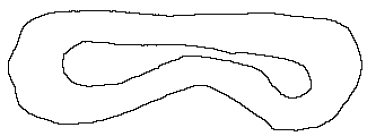
\includegraphics[interpolate=true,width=3.670000in,height=1.360000in]{contents/chapt6/figs/steer/path_method_comparison-img0.png}}%
\end{pgfscope}%
\begin{pgfscope}%
\pgfpathrectangle{\pgfqpoint{0.667277in}{2.634394in}}{\pgfqpoint{3.665446in}{1.471277in}}%
\pgfusepath{clip}%
\pgfsetbuttcap%
\pgfsetroundjoin%
\pgfsetlinewidth{1.505625pt}%
\definecolor{currentstroke}{rgb}{0.501961,0.501961,0.501961}%
\pgfsetstrokecolor{currentstroke}%
\pgfsetdash{{5.550000pt}{2.400000pt}}{0.000000pt}%
\pgfpathmoveto{\pgfqpoint{2.696385in}{3.398736in}}%
\pgfpathlineto{\pgfqpoint{2.806564in}{3.374569in}}%
\pgfpathlineto{\pgfqpoint{2.872154in}{3.357893in}}%
\pgfpathlineto{\pgfqpoint{2.915499in}{3.345172in}}%
\pgfpathlineto{\pgfqpoint{2.958431in}{3.330828in}}%
\pgfpathlineto{\pgfqpoint{3.000795in}{3.314786in}}%
\pgfpathlineto{\pgfqpoint{3.042423in}{3.297023in}}%
\pgfpathlineto{\pgfqpoint{3.083143in}{3.277514in}}%
\pgfpathlineto{\pgfqpoint{3.122787in}{3.256236in}}%
\pgfpathlineto{\pgfqpoint{3.161228in}{3.233161in}}%
\pgfpathlineto{\pgfqpoint{3.198501in}{3.208246in}}%
\pgfpathlineto{\pgfqpoint{3.234685in}{3.181445in}}%
\pgfpathlineto{\pgfqpoint{3.269856in}{3.152711in}}%
\pgfpathlineto{\pgfqpoint{3.304093in}{3.121998in}}%
\pgfpathlineto{\pgfqpoint{3.388304in}{3.042061in}}%
\pgfpathlineto{\pgfqpoint{3.405757in}{3.027513in}}%
\pgfpathlineto{\pgfqpoint{3.423676in}{3.014065in}}%
\pgfpathlineto{\pgfqpoint{3.442176in}{3.001982in}}%
\pgfpathlineto{\pgfqpoint{3.461368in}{2.991531in}}%
\pgfpathlineto{\pgfqpoint{3.481364in}{2.982976in}}%
\pgfpathlineto{\pgfqpoint{3.502217in}{2.976485in}}%
\pgfpathlineto{\pgfqpoint{3.523817in}{2.971970in}}%
\pgfpathlineto{\pgfqpoint{3.546026in}{2.969299in}}%
\pgfpathlineto{\pgfqpoint{3.568710in}{2.968342in}}%
\pgfpathlineto{\pgfqpoint{3.591733in}{2.968969in}}%
\pgfpathlineto{\pgfqpoint{3.614958in}{2.971048in}}%
\pgfpathlineto{\pgfqpoint{3.638250in}{2.974451in}}%
\pgfpathlineto{\pgfqpoint{3.684489in}{2.984700in}}%
\pgfpathlineto{\pgfqpoint{3.729390in}{2.998721in}}%
\pgfpathlineto{\pgfqpoint{3.772262in}{3.016188in}}%
\pgfpathlineto{\pgfqpoint{3.792804in}{3.026263in}}%
\pgfpathlineto{\pgfqpoint{3.812680in}{3.037260in}}%
\pgfpathlineto{\pgfqpoint{3.831840in}{3.049203in}}%
\pgfpathlineto{\pgfqpoint{3.850230in}{3.062111in}}%
\pgfpathlineto{\pgfqpoint{3.867798in}{3.076006in}}%
\pgfpathlineto{\pgfqpoint{3.884493in}{3.090911in}}%
\pgfpathlineto{\pgfqpoint{3.900263in}{3.106844in}}%
\pgfpathlineto{\pgfqpoint{3.915068in}{3.123783in}}%
\pgfpathlineto{\pgfqpoint{3.928885in}{3.141654in}}%
\pgfpathlineto{\pgfqpoint{3.941688in}{3.160381in}}%
\pgfpathlineto{\pgfqpoint{3.953454in}{3.179890in}}%
\pgfpathlineto{\pgfqpoint{3.964158in}{3.200105in}}%
\pgfpathlineto{\pgfqpoint{3.973776in}{3.220950in}}%
\pgfpathlineto{\pgfqpoint{3.982285in}{3.242350in}}%
\pgfpathlineto{\pgfqpoint{3.989659in}{3.264229in}}%
\pgfpathlineto{\pgfqpoint{3.995876in}{3.286512in}}%
\pgfpathlineto{\pgfqpoint{4.000909in}{3.309123in}}%
\pgfpathlineto{\pgfqpoint{4.004722in}{3.331977in}}%
\pgfpathlineto{\pgfqpoint{4.007262in}{3.354976in}}%
\pgfpathlineto{\pgfqpoint{4.008475in}{3.378025in}}%
\pgfpathlineto{\pgfqpoint{4.008310in}{3.401028in}}%
\pgfpathlineto{\pgfqpoint{4.006712in}{3.423886in}}%
\pgfpathlineto{\pgfqpoint{4.003630in}{3.446505in}}%
\pgfpathlineto{\pgfqpoint{3.999011in}{3.468788in}}%
\pgfpathlineto{\pgfqpoint{3.992801in}{3.490637in}}%
\pgfpathlineto{\pgfqpoint{3.984947in}{3.511956in}}%
\pgfpathlineto{\pgfqpoint{3.975407in}{3.532650in}}%
\pgfpathlineto{\pgfqpoint{3.964238in}{3.552628in}}%
\pgfpathlineto{\pgfqpoint{3.951559in}{3.571800in}}%
\pgfpathlineto{\pgfqpoint{3.937491in}{3.590078in}}%
\pgfpathlineto{\pgfqpoint{3.922151in}{3.607376in}}%
\pgfpathlineto{\pgfqpoint{3.905660in}{3.623604in}}%
\pgfpathlineto{\pgfqpoint{3.888138in}{3.638673in}}%
\pgfpathlineto{\pgfqpoint{3.869703in}{3.652497in}}%
\pgfpathlineto{\pgfqpoint{3.850476in}{3.664987in}}%
\pgfpathlineto{\pgfqpoint{3.830575in}{3.676055in}}%
\pgfpathlineto{\pgfqpoint{3.810114in}{3.685643in}}%
\pgfpathlineto{\pgfqpoint{3.789167in}{3.693863in}}%
\pgfpathlineto{\pgfqpoint{3.746068in}{3.706861in}}%
\pgfpathlineto{\pgfqpoint{3.701783in}{3.716371in}}%
\pgfpathlineto{\pgfqpoint{3.634229in}{3.726994in}}%
\pgfpathlineto{\pgfqpoint{3.499771in}{3.747282in}}%
\pgfpathlineto{\pgfqpoint{3.410650in}{3.759452in}}%
\pgfpathlineto{\pgfqpoint{3.343479in}{3.765825in}}%
\pgfpathlineto{\pgfqpoint{3.275935in}{3.769550in}}%
\pgfpathlineto{\pgfqpoint{3.208172in}{3.771173in}}%
\pgfpathlineto{\pgfqpoint{3.117745in}{3.771081in}}%
\pgfpathlineto{\pgfqpoint{3.004905in}{3.770866in}}%
\pgfpathlineto{\pgfqpoint{2.937389in}{3.773198in}}%
\pgfpathlineto{\pgfqpoint{2.870047in}{3.778656in}}%
\pgfpathlineto{\pgfqpoint{2.780393in}{3.789072in}}%
\pgfpathlineto{\pgfqpoint{2.668215in}{3.802389in}}%
\pgfpathlineto{\pgfqpoint{2.600762in}{3.808590in}}%
\pgfpathlineto{\pgfqpoint{2.533230in}{3.812738in}}%
\pgfpathlineto{\pgfqpoint{2.465651in}{3.814315in}}%
\pgfpathlineto{\pgfqpoint{2.398042in}{3.813424in}}%
\pgfpathlineto{\pgfqpoint{2.127202in}{3.806463in}}%
\pgfpathlineto{\pgfqpoint{2.059612in}{3.808894in}}%
\pgfpathlineto{\pgfqpoint{2.014674in}{3.812370in}}%
\pgfpathlineto{\pgfqpoint{1.947422in}{3.819830in}}%
\pgfpathlineto{\pgfqpoint{1.835336in}{3.832723in}}%
\pgfpathlineto{\pgfqpoint{1.790357in}{3.836108in}}%
\pgfpathlineto{\pgfqpoint{1.722703in}{3.838416in}}%
\pgfpathlineto{\pgfqpoint{1.654965in}{3.838187in}}%
\pgfpathlineto{\pgfqpoint{1.564790in}{3.835497in}}%
\pgfpathlineto{\pgfqpoint{1.497368in}{3.831935in}}%
\pgfpathlineto{\pgfqpoint{1.452474in}{3.828139in}}%
\pgfpathlineto{\pgfqpoint{1.407586in}{3.822696in}}%
\pgfpathlineto{\pgfqpoint{1.362671in}{3.815170in}}%
\pgfpathlineto{\pgfqpoint{1.317901in}{3.805078in}}%
\pgfpathlineto{\pgfqpoint{1.273985in}{3.791817in}}%
\pgfpathlineto{\pgfqpoint{1.252598in}{3.783803in}}%
\pgfpathlineto{\pgfqpoint{1.231725in}{3.774764in}}%
\pgfpathlineto{\pgfqpoint{1.211466in}{3.764622in}}%
\pgfpathlineto{\pgfqpoint{1.191920in}{3.753298in}}%
\pgfpathlineto{\pgfqpoint{1.173189in}{3.740715in}}%
\pgfpathlineto{\pgfqpoint{1.155371in}{3.726795in}}%
\pgfpathlineto{\pgfqpoint{1.138551in}{3.711530in}}%
\pgfpathlineto{\pgfqpoint{1.122785in}{3.695025in}}%
\pgfpathlineto{\pgfqpoint{1.108129in}{3.677395in}}%
\pgfpathlineto{\pgfqpoint{1.094637in}{3.658758in}}%
\pgfpathlineto{\pgfqpoint{1.082362in}{3.639229in}}%
\pgfpathlineto{\pgfqpoint{1.071361in}{3.618924in}}%
\pgfpathlineto{\pgfqpoint{1.061686in}{3.597960in}}%
\pgfpathlineto{\pgfqpoint{1.053394in}{3.576453in}}%
\pgfpathlineto{\pgfqpoint{1.046537in}{3.554520in}}%
\pgfpathlineto{\pgfqpoint{1.041170in}{3.532276in}}%
\pgfpathlineto{\pgfqpoint{1.037309in}{3.509813in}}%
\pgfpathlineto{\pgfqpoint{1.034921in}{3.487193in}}%
\pgfpathlineto{\pgfqpoint{1.033973in}{3.464476in}}%
\pgfpathlineto{\pgfqpoint{1.034427in}{3.441723in}}%
\pgfpathlineto{\pgfqpoint{1.036250in}{3.418992in}}%
\pgfpathlineto{\pgfqpoint{1.039405in}{3.396345in}}%
\pgfpathlineto{\pgfqpoint{1.043857in}{3.373840in}}%
\pgfpathlineto{\pgfqpoint{1.049572in}{3.351538in}}%
\pgfpathlineto{\pgfqpoint{1.056513in}{3.329498in}}%
\pgfpathlineto{\pgfqpoint{1.064646in}{3.307783in}}%
\pgfpathlineto{\pgfqpoint{1.073943in}{3.286488in}}%
\pgfpathlineto{\pgfqpoint{1.084382in}{3.265734in}}%
\pgfpathlineto{\pgfqpoint{1.095940in}{3.245641in}}%
\pgfpathlineto{\pgfqpoint{1.108594in}{3.226329in}}%
\pgfpathlineto{\pgfqpoint{1.122323in}{3.207921in}}%
\pgfpathlineto{\pgfqpoint{1.137104in}{3.190535in}}%
\pgfpathlineto{\pgfqpoint{1.152915in}{3.174294in}}%
\pgfpathlineto{\pgfqpoint{1.169733in}{3.159317in}}%
\pgfpathlineto{\pgfqpoint{1.187536in}{3.145727in}}%
\pgfpathlineto{\pgfqpoint{1.206293in}{3.133621in}}%
\pgfpathlineto{\pgfqpoint{1.225924in}{3.122954in}}%
\pgfpathlineto{\pgfqpoint{1.246324in}{3.113617in}}%
\pgfpathlineto{\pgfqpoint{1.267391in}{3.105503in}}%
\pgfpathlineto{\pgfqpoint{1.311107in}{3.092511in}}%
\pgfpathlineto{\pgfqpoint{1.356244in}{3.083112in}}%
\pgfpathlineto{\pgfqpoint{1.401972in}{3.076443in}}%
\pgfpathlineto{\pgfqpoint{1.447588in}{3.071789in}}%
\pgfpathlineto{\pgfqpoint{1.492944in}{3.069111in}}%
\pgfpathlineto{\pgfqpoint{1.538050in}{3.068559in}}%
\pgfpathlineto{\pgfqpoint{1.582915in}{3.070285in}}%
\pgfpathlineto{\pgfqpoint{1.627549in}{3.074438in}}%
\pgfpathlineto{\pgfqpoint{1.671960in}{3.081068in}}%
\pgfpathlineto{\pgfqpoint{1.716156in}{3.089829in}}%
\pgfpathlineto{\pgfqpoint{1.782056in}{3.106001in}}%
\pgfpathlineto{\pgfqpoint{1.869216in}{3.130921in}}%
\pgfpathlineto{\pgfqpoint{1.955457in}{3.157977in}}%
\pgfpathlineto{\pgfqpoint{2.019297in}{3.180176in}}%
\pgfpathlineto{\pgfqpoint{2.082222in}{3.204553in}}%
\pgfpathlineto{\pgfqpoint{2.144271in}{3.231152in}}%
\pgfpathlineto{\pgfqpoint{2.226220in}{3.269095in}}%
\pgfpathlineto{\pgfqpoint{2.349265in}{3.327528in}}%
\pgfpathlineto{\pgfqpoint{2.390888in}{3.345243in}}%
\pgfpathlineto{\pgfqpoint{2.433093in}{3.360813in}}%
\pgfpathlineto{\pgfqpoint{2.476048in}{3.373473in}}%
\pgfpathlineto{\pgfqpoint{2.519846in}{3.382773in}}%
\pgfpathlineto{\pgfqpoint{2.564351in}{3.389250in}}%
\pgfpathlineto{\pgfqpoint{2.609380in}{3.393635in}}%
\pgfpathlineto{\pgfqpoint{2.677505in}{3.397886in}}%
\pgfpathlineto{\pgfqpoint{2.677505in}{3.397886in}}%
\pgfusepath{stroke}%
\end{pgfscope}%
\begin{pgfscope}%
\pgfpathrectangle{\pgfqpoint{0.667277in}{2.634394in}}{\pgfqpoint{3.665446in}{1.471277in}}%
\pgfusepath{clip}%
\pgfsetrectcap%
\pgfsetroundjoin%
\pgfsetlinewidth{1.505625pt}%
\definecolor{currentstroke}{rgb}{0.121569,0.466667,0.705882}%
\pgfsetstrokecolor{currentstroke}%
\pgfsetdash{}{0pt}%
\pgfpathmoveto{\pgfqpoint{2.922936in}{3.767323in}}%
\pgfpathlineto{\pgfqpoint{2.706934in}{3.768407in}}%
\pgfpathlineto{\pgfqpoint{2.628628in}{3.770229in}}%
\pgfpathlineto{\pgfqpoint{2.560968in}{3.774071in}}%
\pgfpathlineto{\pgfqpoint{2.504761in}{3.779547in}}%
\pgfpathlineto{\pgfqpoint{2.403969in}{3.792794in}}%
\pgfpathlineto{\pgfqpoint{2.325512in}{3.802586in}}%
\pgfpathlineto{\pgfqpoint{2.258008in}{3.808580in}}%
\pgfpathlineto{\pgfqpoint{2.066539in}{3.822999in}}%
\pgfpathlineto{\pgfqpoint{1.976812in}{3.833695in}}%
\pgfpathlineto{\pgfqpoint{1.842244in}{3.849922in}}%
\pgfpathlineto{\pgfqpoint{1.774757in}{3.856117in}}%
\pgfpathlineto{\pgfqpoint{1.718390in}{3.859618in}}%
\pgfpathlineto{\pgfqpoint{1.661937in}{3.861145in}}%
\pgfpathlineto{\pgfqpoint{1.605465in}{3.860532in}}%
\pgfpathlineto{\pgfqpoint{1.560341in}{3.858311in}}%
\pgfpathlineto{\pgfqpoint{1.526617in}{3.855035in}}%
\pgfpathlineto{\pgfqpoint{1.493135in}{3.849843in}}%
\pgfpathlineto{\pgfqpoint{1.460095in}{3.842347in}}%
\pgfpathlineto{\pgfqpoint{1.427743in}{3.832296in}}%
\pgfpathlineto{\pgfqpoint{1.396411in}{3.819416in}}%
\pgfpathlineto{\pgfqpoint{1.366439in}{3.803631in}}%
\pgfpathlineto{\pgfqpoint{1.347378in}{3.791512in}}%
\pgfpathlineto{\pgfqpoint{1.329175in}{3.778137in}}%
\pgfpathlineto{\pgfqpoint{1.311971in}{3.763502in}}%
\pgfpathlineto{\pgfqpoint{1.295855in}{3.747675in}}%
\pgfpathlineto{\pgfqpoint{1.280920in}{3.730730in}}%
\pgfpathlineto{\pgfqpoint{1.267255in}{3.712744in}}%
\pgfpathlineto{\pgfqpoint{1.254945in}{3.693807in}}%
\pgfpathlineto{\pgfqpoint{1.244067in}{3.674011in}}%
\pgfpathlineto{\pgfqpoint{1.234690in}{3.653462in}}%
\pgfpathlineto{\pgfqpoint{1.226777in}{3.632306in}}%
\pgfpathlineto{\pgfqpoint{1.220280in}{3.610673in}}%
\pgfpathlineto{\pgfqpoint{1.215224in}{3.588658in}}%
\pgfpathlineto{\pgfqpoint{1.210309in}{3.555141in}}%
\pgfpathlineto{\pgfqpoint{1.208522in}{3.521312in}}%
\pgfpathlineto{\pgfqpoint{1.209859in}{3.487462in}}%
\pgfpathlineto{\pgfqpoint{1.214220in}{3.453868in}}%
\pgfpathlineto{\pgfqpoint{1.221552in}{3.420794in}}%
\pgfpathlineto{\pgfqpoint{1.231906in}{3.388539in}}%
\pgfpathlineto{\pgfqpoint{1.245254in}{3.357406in}}%
\pgfpathlineto{\pgfqpoint{1.261564in}{3.327716in}}%
\pgfpathlineto{\pgfqpoint{1.274063in}{3.308901in}}%
\pgfpathlineto{\pgfqpoint{1.287829in}{3.290993in}}%
\pgfpathlineto{\pgfqpoint{1.302815in}{3.274093in}}%
\pgfpathlineto{\pgfqpoint{1.318964in}{3.258300in}}%
\pgfpathlineto{\pgfqpoint{1.336210in}{3.243714in}}%
\pgfpathlineto{\pgfqpoint{1.363826in}{3.224096in}}%
\pgfpathlineto{\pgfqpoint{1.393104in}{3.207051in}}%
\pgfpathlineto{\pgfqpoint{1.423682in}{3.192466in}}%
\pgfpathlineto{\pgfqpoint{1.455268in}{3.180209in}}%
\pgfpathlineto{\pgfqpoint{1.487606in}{3.170099in}}%
\pgfpathlineto{\pgfqpoint{1.520487in}{3.161921in}}%
\pgfpathlineto{\pgfqpoint{1.553775in}{3.155601in}}%
\pgfpathlineto{\pgfqpoint{1.598549in}{3.149583in}}%
\pgfpathlineto{\pgfqpoint{1.643571in}{3.145829in}}%
\pgfpathlineto{\pgfqpoint{1.688715in}{3.144043in}}%
\pgfpathlineto{\pgfqpoint{1.745188in}{3.144102in}}%
\pgfpathlineto{\pgfqpoint{1.801613in}{3.146436in}}%
\pgfpathlineto{\pgfqpoint{1.846615in}{3.150425in}}%
\pgfpathlineto{\pgfqpoint{1.891374in}{3.156565in}}%
\pgfpathlineto{\pgfqpoint{1.935698in}{3.165289in}}%
\pgfpathlineto{\pgfqpoint{1.968503in}{3.173770in}}%
\pgfpathlineto{\pgfqpoint{2.000833in}{3.183910in}}%
\pgfpathlineto{\pgfqpoint{2.043167in}{3.199682in}}%
\pgfpathlineto{\pgfqpoint{2.095097in}{3.221876in}}%
\pgfpathlineto{\pgfqpoint{2.166714in}{3.255381in}}%
\pgfpathlineto{\pgfqpoint{2.248480in}{3.293841in}}%
\pgfpathlineto{\pgfqpoint{2.290154in}{3.311288in}}%
\pgfpathlineto{\pgfqpoint{2.332636in}{3.326657in}}%
\pgfpathlineto{\pgfqpoint{2.365069in}{3.336462in}}%
\pgfpathlineto{\pgfqpoint{2.397977in}{3.344531in}}%
\pgfpathlineto{\pgfqpoint{2.431279in}{3.350782in}}%
\pgfpathlineto{\pgfqpoint{2.464876in}{3.355171in}}%
\pgfpathlineto{\pgfqpoint{2.498669in}{3.357631in}}%
\pgfpathlineto{\pgfqpoint{2.532547in}{3.358177in}}%
\pgfpathlineto{\pgfqpoint{2.566402in}{3.356807in}}%
\pgfpathlineto{\pgfqpoint{2.600129in}{3.353566in}}%
\pgfpathlineto{\pgfqpoint{2.633625in}{3.348460in}}%
\pgfpathlineto{\pgfqpoint{2.677812in}{3.339058in}}%
\pgfpathlineto{\pgfqpoint{2.721472in}{3.327447in}}%
\pgfpathlineto{\pgfqpoint{2.775331in}{3.310462in}}%
\pgfpathlineto{\pgfqpoint{2.839086in}{3.287486in}}%
\pgfpathlineto{\pgfqpoint{2.912537in}{3.258221in}}%
\pgfpathlineto{\pgfqpoint{2.995594in}{3.222628in}}%
\pgfpathlineto{\pgfqpoint{3.077864in}{3.185253in}}%
\pgfpathlineto{\pgfqpoint{3.148962in}{3.150662in}}%
\pgfpathlineto{\pgfqpoint{3.209010in}{3.119244in}}%
\pgfpathlineto{\pgfqpoint{3.267874in}{3.085662in}}%
\pgfpathlineto{\pgfqpoint{3.346004in}{3.040269in}}%
\pgfpathlineto{\pgfqpoint{3.386252in}{3.019750in}}%
\pgfpathlineto{\pgfqpoint{3.417314in}{3.006219in}}%
\pgfpathlineto{\pgfqpoint{3.449183in}{2.994717in}}%
\pgfpathlineto{\pgfqpoint{3.481804in}{2.985571in}}%
\pgfpathlineto{\pgfqpoint{3.515055in}{2.979086in}}%
\pgfpathlineto{\pgfqpoint{3.548734in}{2.975425in}}%
\pgfpathlineto{\pgfqpoint{3.582604in}{2.974717in}}%
\pgfpathlineto{\pgfqpoint{3.616397in}{2.977095in}}%
\pgfpathlineto{\pgfqpoint{3.649828in}{2.982560in}}%
\pgfpathlineto{\pgfqpoint{3.682587in}{2.991184in}}%
\pgfpathlineto{\pgfqpoint{3.703878in}{2.998728in}}%
\pgfpathlineto{\pgfqpoint{3.724593in}{3.007732in}}%
\pgfpathlineto{\pgfqpoint{3.744608in}{3.018200in}}%
\pgfpathlineto{\pgfqpoint{3.763804in}{3.030105in}}%
\pgfpathlineto{\pgfqpoint{3.782053in}{3.043413in}}%
\pgfpathlineto{\pgfqpoint{3.799230in}{3.058079in}}%
\pgfpathlineto{\pgfqpoint{3.815209in}{3.074043in}}%
\pgfpathlineto{\pgfqpoint{3.829868in}{3.091226in}}%
\pgfpathlineto{\pgfqpoint{3.843096in}{3.109533in}}%
\pgfpathlineto{\pgfqpoint{3.854791in}{3.128856in}}%
\pgfpathlineto{\pgfqpoint{3.864860in}{3.149073in}}%
\pgfpathlineto{\pgfqpoint{3.873226in}{3.170052in}}%
\pgfpathlineto{\pgfqpoint{3.879823in}{3.191653in}}%
\pgfpathlineto{\pgfqpoint{3.884599in}{3.213729in}}%
\pgfpathlineto{\pgfqpoint{3.887515in}{3.236125in}}%
\pgfpathlineto{\pgfqpoint{3.888549in}{3.258688in}}%
\pgfpathlineto{\pgfqpoint{3.887690in}{3.281257in}}%
\pgfpathlineto{\pgfqpoint{3.884942in}{3.303675in}}%
\pgfpathlineto{\pgfqpoint{3.880324in}{3.325784in}}%
\pgfpathlineto{\pgfqpoint{3.873866in}{3.347427in}}%
\pgfpathlineto{\pgfqpoint{3.865649in}{3.368465in}}%
\pgfpathlineto{\pgfqpoint{3.855848in}{3.388815in}}%
\pgfpathlineto{\pgfqpoint{3.844638in}{3.408426in}}%
\pgfpathlineto{\pgfqpoint{3.825510in}{3.436384in}}%
\pgfpathlineto{\pgfqpoint{3.803905in}{3.462477in}}%
\pgfpathlineto{\pgfqpoint{3.780129in}{3.486611in}}%
\pgfpathlineto{\pgfqpoint{3.754527in}{3.508799in}}%
\pgfpathlineto{\pgfqpoint{3.727371in}{3.529060in}}%
\pgfpathlineto{\pgfqpoint{3.699041in}{3.547645in}}%
\pgfpathlineto{\pgfqpoint{3.669744in}{3.564668in}}%
\pgfpathlineto{\pgfqpoint{3.629448in}{3.585089in}}%
\pgfpathlineto{\pgfqpoint{3.588049in}{3.603176in}}%
\pgfpathlineto{\pgfqpoint{3.545794in}{3.619161in}}%
\pgfpathlineto{\pgfqpoint{3.492080in}{3.636601in}}%
\pgfpathlineto{\pgfqpoint{3.437743in}{3.651992in}}%
\pgfpathlineto{\pgfqpoint{3.382930in}{3.665594in}}%
\pgfpathlineto{\pgfqpoint{3.316665in}{3.679795in}}%
\pgfpathlineto{\pgfqpoint{3.238902in}{3.694091in}}%
\pgfpathlineto{\pgfqpoint{3.149626in}{3.708058in}}%
\pgfpathlineto{\pgfqpoint{3.026481in}{3.724594in}}%
\pgfpathlineto{\pgfqpoint{2.925842in}{3.738943in}}%
\pgfpathlineto{\pgfqpoint{2.914686in}{3.740711in}}%
\pgfpathlineto{\pgfqpoint{2.914686in}{3.740711in}}%
\pgfusepath{stroke}%
\end{pgfscope}%
\begin{pgfscope}%
\pgfpathrectangle{\pgfqpoint{0.667277in}{2.634394in}}{\pgfqpoint{3.665446in}{1.471277in}}%
\pgfusepath{clip}%
\pgfsetbuttcap%
\pgfsetroundjoin%
\pgfsetlinewidth{1.505625pt}%
\definecolor{currentstroke}{rgb}{1.000000,0.000000,0.000000}%
\pgfsetstrokecolor{currentstroke}%
\pgfsetstrokeopacity{0.500000}%
\pgfsetdash{{9.600000pt}{2.400000pt}{1.500000pt}{2.400000pt}}{0.000000pt}%
\pgfpathmoveto{\pgfqpoint{2.877824in}{3.767565in}}%
\pgfpathlineto{\pgfqpoint{2.855267in}{3.767686in}}%
\pgfpathlineto{\pgfqpoint{2.832711in}{3.767807in}}%
\pgfpathlineto{\pgfqpoint{2.810155in}{3.767928in}}%
\pgfpathlineto{\pgfqpoint{2.787599in}{3.768049in}}%
\pgfpathlineto{\pgfqpoint{2.765042in}{3.768170in}}%
\pgfpathlineto{\pgfqpoint{2.742486in}{3.768291in}}%
\pgfpathlineto{\pgfqpoint{2.719930in}{3.768412in}}%
\pgfpathlineto{\pgfqpoint{2.697373in}{3.768533in}}%
\pgfpathlineto{\pgfqpoint{2.674817in}{3.768654in}}%
\pgfpathlineto{\pgfqpoint{2.652261in}{3.768775in}}%
\pgfpathlineto{\pgfqpoint{2.629705in}{3.768896in}}%
\pgfpathlineto{\pgfqpoint{2.607148in}{3.769017in}}%
\pgfpathlineto{\pgfqpoint{2.584592in}{3.769138in}}%
\pgfpathlineto{\pgfqpoint{2.562036in}{3.769259in}}%
\pgfpathlineto{\pgfqpoint{2.539480in}{3.769380in}}%
\pgfpathlineto{\pgfqpoint{2.516923in}{3.769501in}}%
\pgfpathlineto{\pgfqpoint{2.494367in}{3.769623in}}%
\pgfpathlineto{\pgfqpoint{2.471811in}{3.769744in}}%
\pgfpathlineto{\pgfqpoint{2.449254in}{3.769865in}}%
\pgfpathlineto{\pgfqpoint{2.426698in}{3.769986in}}%
\pgfpathlineto{\pgfqpoint{2.404142in}{3.770107in}}%
\pgfpathlineto{\pgfqpoint{2.381586in}{3.770228in}}%
\pgfpathlineto{\pgfqpoint{2.359029in}{3.770349in}}%
\pgfpathlineto{\pgfqpoint{2.336473in}{3.770470in}}%
\pgfpathlineto{\pgfqpoint{2.313917in}{3.770591in}}%
\pgfpathlineto{\pgfqpoint{2.291361in}{3.770712in}}%
\pgfpathlineto{\pgfqpoint{2.268804in}{3.770833in}}%
\pgfpathlineto{\pgfqpoint{2.246248in}{3.770954in}}%
\pgfpathlineto{\pgfqpoint{2.223692in}{3.771075in}}%
\pgfpathlineto{\pgfqpoint{2.201136in}{3.771196in}}%
\pgfpathlineto{\pgfqpoint{2.178579in}{3.771317in}}%
\pgfpathlineto{\pgfqpoint{2.156023in}{3.771438in}}%
\pgfpathlineto{\pgfqpoint{2.133467in}{3.771559in}}%
\pgfpathlineto{\pgfqpoint{2.110910in}{3.771680in}}%
\pgfpathlineto{\pgfqpoint{2.088354in}{3.771801in}}%
\pgfusepath{stroke}%
\end{pgfscope}%
\begin{pgfscope}%
\pgfpathrectangle{\pgfqpoint{0.667277in}{2.634394in}}{\pgfqpoint{3.665446in}{1.471277in}}%
\pgfusepath{clip}%
\pgfsetrectcap%
\pgfsetroundjoin%
\pgfsetlinewidth{1.505625pt}%
\definecolor{currentstroke}{rgb}{1.000000,0.000000,0.000000}%
\pgfsetstrokecolor{currentstroke}%
\pgfsetstrokeopacity{0.500000}%
\pgfsetdash{}{0pt}%
\pgfpathmoveto{\pgfqpoint{2.877824in}{3.767565in}}%
\pgfusepath{stroke}%
\end{pgfscope}%
\begin{pgfscope}%
\pgfpathrectangle{\pgfqpoint{0.667277in}{2.634394in}}{\pgfqpoint{3.665446in}{1.471277in}}%
\pgfusepath{clip}%
\pgfsetbuttcap%
\pgfsetmiterjoin%
\definecolor{currentfill}{rgb}{1.000000,0.000000,0.000000}%
\pgfsetfillcolor{currentfill}%
\pgfsetfillopacity{0.500000}%
\pgfsetlinewidth{1.003750pt}%
\definecolor{currentstroke}{rgb}{1.000000,0.000000,0.000000}%
\pgfsetstrokecolor{currentstroke}%
\pgfsetstrokeopacity{0.500000}%
\pgfsetdash{}{0pt}%
\pgfsys@defobject{currentmarker}{\pgfqpoint{-0.041667in}{-0.041667in}}{\pgfqpoint{0.041667in}{0.041667in}}{%
\pgfpathmoveto{\pgfqpoint{-0.041667in}{-0.041667in}}%
\pgfpathlineto{\pgfqpoint{0.041667in}{-0.041667in}}%
\pgfpathlineto{\pgfqpoint{0.041667in}{0.041667in}}%
\pgfpathlineto{\pgfqpoint{-0.041667in}{0.041667in}}%
\pgfpathlineto{\pgfqpoint{-0.041667in}{-0.041667in}}%
\pgfpathclose%
\pgfusepath{stroke,fill}%
}%
\begin{pgfscope}%
\pgfsys@transformshift{2.877824in}{3.767565in}%
\pgfsys@useobject{currentmarker}{}%
\end{pgfscope}%
\end{pgfscope}%
\begin{pgfscope}%
\pgfpathrectangle{\pgfqpoint{0.667277in}{2.634394in}}{\pgfqpoint{3.665446in}{1.471277in}}%
\pgfusepath{clip}%
\pgfsetbuttcap%
\pgfsetroundjoin%
\pgfsetlinewidth{1.505625pt}%
\definecolor{currentstroke}{rgb}{1.000000,0.000000,0.000000}%
\pgfsetstrokecolor{currentstroke}%
\pgfsetstrokeopacity{0.500000}%
\pgfsetdash{{9.600000pt}{2.400000pt}{1.500000pt}{2.400000pt}}{0.000000pt}%
\pgfpathmoveto{\pgfqpoint{2.518077in}{3.778396in}}%
\pgfpathlineto{\pgfqpoint{2.495723in}{3.781412in}}%
\pgfpathlineto{\pgfqpoint{2.473331in}{3.784131in}}%
\pgfpathlineto{\pgfqpoint{2.450905in}{3.786554in}}%
\pgfpathlineto{\pgfqpoint{2.428449in}{3.788679in}}%
\pgfpathlineto{\pgfqpoint{2.405967in}{3.790507in}}%
\pgfpathlineto{\pgfqpoint{2.383462in}{3.792036in}}%
\pgfpathlineto{\pgfqpoint{2.360939in}{3.793268in}}%
\pgfpathlineto{\pgfqpoint{2.338402in}{3.794201in}}%
\pgfpathlineto{\pgfqpoint{2.315855in}{3.794835in}}%
\pgfpathlineto{\pgfqpoint{2.293301in}{3.795171in}}%
\pgfpathlineto{\pgfqpoint{2.270744in}{3.795208in}}%
\pgfpathlineto{\pgfqpoint{2.248189in}{3.794946in}}%
\pgfpathlineto{\pgfqpoint{2.225640in}{3.794386in}}%
\pgfpathlineto{\pgfqpoint{2.203100in}{3.793526in}}%
\pgfpathlineto{\pgfqpoint{2.180573in}{3.792369in}}%
\pgfpathlineto{\pgfqpoint{2.158064in}{3.790913in}}%
\pgfpathlineto{\pgfqpoint{2.135575in}{3.789159in}}%
\pgfpathlineto{\pgfqpoint{2.113112in}{3.787107in}}%
\pgfpathlineto{\pgfqpoint{2.090679in}{3.784756in}}%
\pgfpathlineto{\pgfqpoint{2.068264in}{3.782236in}}%
\pgfpathlineto{\pgfqpoint{2.045846in}{3.779733in}}%
\pgfpathlineto{\pgfqpoint{2.023429in}{3.777230in}}%
\pgfpathlineto{\pgfqpoint{2.001012in}{3.774721in}}%
\pgfpathlineto{\pgfqpoint{1.978596in}{3.772211in}}%
\pgfpathlineto{\pgfqpoint{1.956179in}{3.769703in}}%
\pgfpathlineto{\pgfqpoint{1.933762in}{3.767196in}}%
\pgfpathlineto{\pgfqpoint{1.911346in}{3.764688in}}%
\pgfpathlineto{\pgfqpoint{1.888929in}{3.762179in}}%
\pgfpathlineto{\pgfqpoint{1.866512in}{3.759671in}}%
\pgfpathlineto{\pgfqpoint{1.844095in}{3.757163in}}%
\pgfpathlineto{\pgfqpoint{1.821679in}{3.754655in}}%
\pgfpathlineto{\pgfqpoint{1.799262in}{3.752147in}}%
\pgfpathlineto{\pgfqpoint{1.776845in}{3.749639in}}%
\pgfpathlineto{\pgfqpoint{1.754429in}{3.747131in}}%
\pgfpathlineto{\pgfqpoint{1.732012in}{3.744623in}}%
\pgfpathlineto{\pgfqpoint{1.709595in}{3.742115in}}%
\pgfpathlineto{\pgfqpoint{1.687178in}{3.739607in}}%
\pgfusepath{stroke}%
\end{pgfscope}%
\begin{pgfscope}%
\pgfpathrectangle{\pgfqpoint{0.667277in}{2.634394in}}{\pgfqpoint{3.665446in}{1.471277in}}%
\pgfusepath{clip}%
\pgfsetrectcap%
\pgfsetroundjoin%
\pgfsetlinewidth{1.505625pt}%
\definecolor{currentstroke}{rgb}{1.000000,0.000000,0.000000}%
\pgfsetstrokecolor{currentstroke}%
\pgfsetstrokeopacity{0.500000}%
\pgfsetdash{}{0pt}%
\pgfpathmoveto{\pgfqpoint{2.518077in}{3.778396in}}%
\pgfusepath{stroke}%
\end{pgfscope}%
\begin{pgfscope}%
\pgfpathrectangle{\pgfqpoint{0.667277in}{2.634394in}}{\pgfqpoint{3.665446in}{1.471277in}}%
\pgfusepath{clip}%
\pgfsetbuttcap%
\pgfsetmiterjoin%
\definecolor{currentfill}{rgb}{1.000000,0.000000,0.000000}%
\pgfsetfillcolor{currentfill}%
\pgfsetfillopacity{0.500000}%
\pgfsetlinewidth{1.003750pt}%
\definecolor{currentstroke}{rgb}{1.000000,0.000000,0.000000}%
\pgfsetstrokecolor{currentstroke}%
\pgfsetstrokeopacity{0.500000}%
\pgfsetdash{}{0pt}%
\pgfsys@defobject{currentmarker}{\pgfqpoint{-0.041667in}{-0.041667in}}{\pgfqpoint{0.041667in}{0.041667in}}{%
\pgfpathmoveto{\pgfqpoint{-0.041667in}{-0.041667in}}%
\pgfpathlineto{\pgfqpoint{0.041667in}{-0.041667in}}%
\pgfpathlineto{\pgfqpoint{0.041667in}{0.041667in}}%
\pgfpathlineto{\pgfqpoint{-0.041667in}{0.041667in}}%
\pgfpathlineto{\pgfqpoint{-0.041667in}{-0.041667in}}%
\pgfpathclose%
\pgfusepath{stroke,fill}%
}%
\begin{pgfscope}%
\pgfsys@transformshift{2.518077in}{3.778396in}%
\pgfsys@useobject{currentmarker}{}%
\end{pgfscope}%
\end{pgfscope}%
\begin{pgfscope}%
\pgfpathrectangle{\pgfqpoint{0.667277in}{2.634394in}}{\pgfqpoint{3.665446in}{1.471277in}}%
\pgfusepath{clip}%
\pgfsetbuttcap%
\pgfsetroundjoin%
\pgfsetlinewidth{1.505625pt}%
\definecolor{currentstroke}{rgb}{1.000000,0.000000,0.000000}%
\pgfsetstrokecolor{currentstroke}%
\pgfsetstrokeopacity{0.500000}%
\pgfsetdash{{9.600000pt}{2.400000pt}{1.500000pt}{2.400000pt}}{0.000000pt}%
\pgfpathmoveto{\pgfqpoint{2.068643in}{3.823054in}}%
\pgfpathlineto{\pgfqpoint{2.046266in}{3.825889in}}%
\pgfpathlineto{\pgfqpoint{2.023873in}{3.828601in}}%
\pgfpathlineto{\pgfqpoint{2.001465in}{3.831189in}}%
\pgfpathlineto{\pgfqpoint{1.979044in}{3.833654in}}%
\pgfpathlineto{\pgfqpoint{1.956609in}{3.835995in}}%
\pgfpathlineto{\pgfqpoint{1.934161in}{3.838212in}}%
\pgfpathlineto{\pgfqpoint{1.911702in}{3.840305in}}%
\pgfpathlineto{\pgfqpoint{1.889232in}{3.842275in}}%
\pgfpathlineto{\pgfqpoint{1.866751in}{3.844120in}}%
\pgfpathlineto{\pgfqpoint{1.844260in}{3.845842in}}%
\pgfpathlineto{\pgfqpoint{1.821760in}{3.847440in}}%
\pgfpathlineto{\pgfqpoint{1.799252in}{3.848913in}}%
\pgfpathlineto{\pgfqpoint{1.776736in}{3.850263in}}%
\pgfpathlineto{\pgfqpoint{1.754212in}{3.851488in}}%
\pgfpathlineto{\pgfqpoint{1.731683in}{3.852590in}}%
\pgfpathlineto{\pgfqpoint{1.709147in}{3.853567in}}%
\pgfpathlineto{\pgfqpoint{1.686607in}{3.854419in}}%
\pgfpathlineto{\pgfqpoint{1.664062in}{3.855148in}}%
\pgfpathlineto{\pgfqpoint{1.641514in}{3.855751in}}%
\pgfpathlineto{\pgfqpoint{1.618963in}{3.856289in}}%
\pgfpathlineto{\pgfqpoint{1.596413in}{3.856835in}}%
\pgfpathlineto{\pgfqpoint{1.573863in}{3.857380in}}%
\pgfpathlineto{\pgfqpoint{1.551313in}{3.857923in}}%
\pgfpathlineto{\pgfqpoint{1.528763in}{3.858466in}}%
\pgfpathlineto{\pgfqpoint{1.506213in}{3.859009in}}%
\pgfpathlineto{\pgfqpoint{1.483663in}{3.859553in}}%
\pgfpathlineto{\pgfqpoint{1.461113in}{3.860096in}}%
\pgfpathlineto{\pgfqpoint{1.438563in}{3.860639in}}%
\pgfpathlineto{\pgfqpoint{1.416013in}{3.861183in}}%
\pgfpathlineto{\pgfqpoint{1.393463in}{3.861726in}}%
\pgfpathlineto{\pgfqpoint{1.370913in}{3.862269in}}%
\pgfpathlineto{\pgfqpoint{1.348363in}{3.862813in}}%
\pgfpathlineto{\pgfqpoint{1.325813in}{3.863356in}}%
\pgfpathlineto{\pgfqpoint{1.303263in}{3.863899in}}%
\pgfpathlineto{\pgfqpoint{1.280713in}{3.864443in}}%
\pgfpathlineto{\pgfqpoint{1.258163in}{3.864986in}}%
\pgfusepath{stroke}%
\end{pgfscope}%
\begin{pgfscope}%
\pgfpathrectangle{\pgfqpoint{0.667277in}{2.634394in}}{\pgfqpoint{3.665446in}{1.471277in}}%
\pgfusepath{clip}%
\pgfsetrectcap%
\pgfsetroundjoin%
\pgfsetlinewidth{1.505625pt}%
\definecolor{currentstroke}{rgb}{1.000000,0.000000,0.000000}%
\pgfsetstrokecolor{currentstroke}%
\pgfsetstrokeopacity{0.500000}%
\pgfsetdash{}{0pt}%
\pgfpathmoveto{\pgfqpoint{2.068643in}{3.823054in}}%
\pgfusepath{stroke}%
\end{pgfscope}%
\begin{pgfscope}%
\pgfpathrectangle{\pgfqpoint{0.667277in}{2.634394in}}{\pgfqpoint{3.665446in}{1.471277in}}%
\pgfusepath{clip}%
\pgfsetbuttcap%
\pgfsetmiterjoin%
\definecolor{currentfill}{rgb}{1.000000,0.000000,0.000000}%
\pgfsetfillcolor{currentfill}%
\pgfsetfillopacity{0.500000}%
\pgfsetlinewidth{1.003750pt}%
\definecolor{currentstroke}{rgb}{1.000000,0.000000,0.000000}%
\pgfsetstrokecolor{currentstroke}%
\pgfsetstrokeopacity{0.500000}%
\pgfsetdash{}{0pt}%
\pgfsys@defobject{currentmarker}{\pgfqpoint{-0.041667in}{-0.041667in}}{\pgfqpoint{0.041667in}{0.041667in}}{%
\pgfpathmoveto{\pgfqpoint{-0.041667in}{-0.041667in}}%
\pgfpathlineto{\pgfqpoint{0.041667in}{-0.041667in}}%
\pgfpathlineto{\pgfqpoint{0.041667in}{0.041667in}}%
\pgfpathlineto{\pgfqpoint{-0.041667in}{0.041667in}}%
\pgfpathlineto{\pgfqpoint{-0.041667in}{-0.041667in}}%
\pgfpathclose%
\pgfusepath{stroke,fill}%
}%
\begin{pgfscope}%
\pgfsys@transformshift{2.068643in}{3.823054in}%
\pgfsys@useobject{currentmarker}{}%
\end{pgfscope}%
\end{pgfscope}%
\begin{pgfscope}%
\pgfpathrectangle{\pgfqpoint{0.667277in}{2.634394in}}{\pgfqpoint{3.665446in}{1.471277in}}%
\pgfusepath{clip}%
\pgfsetbuttcap%
\pgfsetroundjoin%
\pgfsetlinewidth{1.505625pt}%
\definecolor{currentstroke}{rgb}{1.000000,0.000000,0.000000}%
\pgfsetstrokecolor{currentstroke}%
\pgfsetstrokeopacity{0.500000}%
\pgfsetdash{{9.600000pt}{2.400000pt}{1.500000pt}{2.400000pt}}{0.000000pt}%
\pgfpathmoveto{\pgfqpoint{1.617771in}{3.860196in}}%
\pgfpathlineto{\pgfqpoint{1.595418in}{3.857206in}}%
\pgfpathlineto{\pgfqpoint{1.573341in}{3.852599in}}%
\pgfpathlineto{\pgfqpoint{1.551658in}{3.846397in}}%
\pgfpathlineto{\pgfqpoint{1.530483in}{3.838634in}}%
\pgfpathlineto{\pgfqpoint{1.509930in}{3.829351in}}%
\pgfpathlineto{\pgfqpoint{1.490106in}{3.818597in}}%
\pgfpathlineto{\pgfqpoint{1.471118in}{3.806429in}}%
\pgfpathlineto{\pgfqpoint{1.453065in}{3.792912in}}%
\pgfpathlineto{\pgfqpoint{1.436043in}{3.778117in}}%
\pgfpathlineto{\pgfqpoint{1.420143in}{3.762123in}}%
\pgfpathlineto{\pgfqpoint{1.405449in}{3.745014in}}%
\pgfpathlineto{\pgfqpoint{1.392038in}{3.726882in}}%
\pgfpathlineto{\pgfqpoint{1.379982in}{3.707822in}}%
\pgfpathlineto{\pgfqpoint{1.369345in}{3.687936in}}%
\pgfpathlineto{\pgfqpoint{1.360183in}{3.667328in}}%
\pgfpathlineto{\pgfqpoint{1.352545in}{3.646108in}}%
\pgfpathlineto{\pgfqpoint{1.346471in}{3.624389in}}%
\pgfpathlineto{\pgfqpoint{1.341993in}{3.602285in}}%
\pgfpathlineto{\pgfqpoint{1.339135in}{3.579914in}}%
\pgfpathlineto{\pgfqpoint{1.337912in}{3.557395in}}%
\pgfpathlineto{\pgfqpoint{1.338330in}{3.534846in}}%
\pgfpathlineto{\pgfqpoint{1.340027in}{3.512353in}}%
\pgfpathlineto{\pgfqpoint{1.341680in}{3.489857in}}%
\pgfpathlineto{\pgfqpoint{1.343304in}{3.467359in}}%
\pgfpathlineto{\pgfqpoint{1.344965in}{3.444864in}}%
\pgfpathlineto{\pgfqpoint{1.346641in}{3.422370in}}%
\pgfpathlineto{\pgfqpoint{1.348308in}{3.399875in}}%
\pgfpathlineto{\pgfqpoint{1.349969in}{3.377380in}}%
\pgfpathlineto{\pgfqpoint{1.351632in}{3.354884in}}%
\pgfpathlineto{\pgfqpoint{1.353297in}{3.332389in}}%
\pgfpathlineto{\pgfqpoint{1.354961in}{3.309894in}}%
\pgfpathlineto{\pgfqpoint{1.356625in}{3.287399in}}%
\pgfpathlineto{\pgfqpoint{1.358289in}{3.264904in}}%
\pgfpathlineto{\pgfqpoint{1.359954in}{3.242409in}}%
\pgfpathlineto{\pgfqpoint{1.361618in}{3.219914in}}%
\pgfpathlineto{\pgfqpoint{1.363282in}{3.197419in}}%
\pgfpathlineto{\pgfqpoint{1.364946in}{3.174923in}}%
\pgfpathlineto{\pgfqpoint{1.366610in}{3.152428in}}%
\pgfpathlineto{\pgfqpoint{1.368274in}{3.129933in}}%
\pgfusepath{stroke}%
\end{pgfscope}%
\begin{pgfscope}%
\pgfpathrectangle{\pgfqpoint{0.667277in}{2.634394in}}{\pgfqpoint{3.665446in}{1.471277in}}%
\pgfusepath{clip}%
\pgfsetrectcap%
\pgfsetroundjoin%
\pgfsetlinewidth{1.505625pt}%
\definecolor{currentstroke}{rgb}{1.000000,0.000000,0.000000}%
\pgfsetstrokecolor{currentstroke}%
\pgfsetstrokeopacity{0.500000}%
\pgfsetdash{}{0pt}%
\pgfpathmoveto{\pgfqpoint{1.617771in}{3.860196in}}%
\pgfusepath{stroke}%
\end{pgfscope}%
\begin{pgfscope}%
\pgfpathrectangle{\pgfqpoint{0.667277in}{2.634394in}}{\pgfqpoint{3.665446in}{1.471277in}}%
\pgfusepath{clip}%
\pgfsetbuttcap%
\pgfsetmiterjoin%
\definecolor{currentfill}{rgb}{1.000000,0.000000,0.000000}%
\pgfsetfillcolor{currentfill}%
\pgfsetfillopacity{0.500000}%
\pgfsetlinewidth{1.003750pt}%
\definecolor{currentstroke}{rgb}{1.000000,0.000000,0.000000}%
\pgfsetstrokecolor{currentstroke}%
\pgfsetstrokeopacity{0.500000}%
\pgfsetdash{}{0pt}%
\pgfsys@defobject{currentmarker}{\pgfqpoint{-0.041667in}{-0.041667in}}{\pgfqpoint{0.041667in}{0.041667in}}{%
\pgfpathmoveto{\pgfqpoint{-0.041667in}{-0.041667in}}%
\pgfpathlineto{\pgfqpoint{0.041667in}{-0.041667in}}%
\pgfpathlineto{\pgfqpoint{0.041667in}{0.041667in}}%
\pgfpathlineto{\pgfqpoint{-0.041667in}{0.041667in}}%
\pgfpathlineto{\pgfqpoint{-0.041667in}{-0.041667in}}%
\pgfpathclose%
\pgfusepath{stroke,fill}%
}%
\begin{pgfscope}%
\pgfsys@transformshift{1.617771in}{3.860196in}%
\pgfsys@useobject{currentmarker}{}%
\end{pgfscope}%
\end{pgfscope}%
\begin{pgfscope}%
\pgfpathrectangle{\pgfqpoint{0.667277in}{2.634394in}}{\pgfqpoint{3.665446in}{1.471277in}}%
\pgfusepath{clip}%
\pgfsetbuttcap%
\pgfsetroundjoin%
\pgfsetlinewidth{1.505625pt}%
\definecolor{currentstroke}{rgb}{1.000000,0.000000,0.000000}%
\pgfsetstrokecolor{currentstroke}%
\pgfsetstrokeopacity{0.500000}%
\pgfsetdash{{9.600000pt}{2.400000pt}{1.500000pt}{2.400000pt}}{0.000000pt}%
\pgfpathmoveto{\pgfqpoint{1.241784in}{3.664295in}}%
\pgfpathlineto{\pgfqpoint{1.237640in}{3.642126in}}%
\pgfpathlineto{\pgfqpoint{1.234913in}{3.619738in}}%
\pgfpathlineto{\pgfqpoint{1.233617in}{3.597221in}}%
\pgfpathlineto{\pgfqpoint{1.233757in}{3.574668in}}%
\pgfpathlineto{\pgfqpoint{1.235332in}{3.552170in}}%
\pgfpathlineto{\pgfqpoint{1.238336in}{3.529817in}}%
\pgfpathlineto{\pgfqpoint{1.242756in}{3.507701in}}%
\pgfpathlineto{\pgfqpoint{1.248574in}{3.485911in}}%
\pgfpathlineto{\pgfqpoint{1.255768in}{3.464536in}}%
\pgfpathlineto{\pgfqpoint{1.264307in}{3.443661in}}%
\pgfpathlineto{\pgfqpoint{1.274158in}{3.423373in}}%
\pgfpathlineto{\pgfqpoint{1.285280in}{3.403752in}}%
\pgfpathlineto{\pgfqpoint{1.297628in}{3.384879in}}%
\pgfpathlineto{\pgfqpoint{1.311152in}{3.366830in}}%
\pgfpathlineto{\pgfqpoint{1.325797in}{3.349678in}}%
\pgfpathlineto{\pgfqpoint{1.341504in}{3.333494in}}%
\pgfpathlineto{\pgfqpoint{1.358209in}{3.318341in}}%
\pgfpathlineto{\pgfqpoint{1.375845in}{3.304283in}}%
\pgfpathlineto{\pgfqpoint{1.394340in}{3.291375in}}%
\pgfpathlineto{\pgfqpoint{1.413618in}{3.279669in}}%
\pgfpathlineto{\pgfqpoint{1.433569in}{3.269149in}}%
\pgfpathlineto{\pgfqpoint{1.453614in}{3.258805in}}%
\pgfpathlineto{\pgfqpoint{1.473634in}{3.248413in}}%
\pgfpathlineto{\pgfqpoint{1.493665in}{3.238043in}}%
\pgfpathlineto{\pgfqpoint{1.513706in}{3.227691in}}%
\pgfpathlineto{\pgfqpoint{1.533745in}{3.217335in}}%
\pgfpathlineto{\pgfqpoint{1.553781in}{3.206974in}}%
\pgfpathlineto{\pgfqpoint{1.573817in}{3.196612in}}%
\pgfpathlineto{\pgfqpoint{1.593854in}{3.186253in}}%
\pgfpathlineto{\pgfqpoint{1.613891in}{3.175893in}}%
\pgfpathlineto{\pgfqpoint{1.633928in}{3.165533in}}%
\pgfpathlineto{\pgfqpoint{1.653965in}{3.155173in}}%
\pgfpathlineto{\pgfqpoint{1.674001in}{3.144813in}}%
\pgfpathlineto{\pgfqpoint{1.694038in}{3.134454in}}%
\pgfpathlineto{\pgfqpoint{1.714075in}{3.124094in}}%
\pgfpathlineto{\pgfqpoint{1.734112in}{3.113734in}}%
\pgfpathlineto{\pgfqpoint{1.754149in}{3.103374in}}%
\pgfpathlineto{\pgfqpoint{1.774185in}{3.093014in}}%
\pgfusepath{stroke}%
\end{pgfscope}%
\begin{pgfscope}%
\pgfpathrectangle{\pgfqpoint{0.667277in}{2.634394in}}{\pgfqpoint{3.665446in}{1.471277in}}%
\pgfusepath{clip}%
\pgfsetrectcap%
\pgfsetroundjoin%
\pgfsetlinewidth{1.505625pt}%
\definecolor{currentstroke}{rgb}{1.000000,0.000000,0.000000}%
\pgfsetstrokecolor{currentstroke}%
\pgfsetstrokeopacity{0.500000}%
\pgfsetdash{}{0pt}%
\pgfpathmoveto{\pgfqpoint{1.241784in}{3.664295in}}%
\pgfusepath{stroke}%
\end{pgfscope}%
\begin{pgfscope}%
\pgfpathrectangle{\pgfqpoint{0.667277in}{2.634394in}}{\pgfqpoint{3.665446in}{1.471277in}}%
\pgfusepath{clip}%
\pgfsetbuttcap%
\pgfsetmiterjoin%
\definecolor{currentfill}{rgb}{1.000000,0.000000,0.000000}%
\pgfsetfillcolor{currentfill}%
\pgfsetfillopacity{0.500000}%
\pgfsetlinewidth{1.003750pt}%
\definecolor{currentstroke}{rgb}{1.000000,0.000000,0.000000}%
\pgfsetstrokecolor{currentstroke}%
\pgfsetstrokeopacity{0.500000}%
\pgfsetdash{}{0pt}%
\pgfsys@defobject{currentmarker}{\pgfqpoint{-0.041667in}{-0.041667in}}{\pgfqpoint{0.041667in}{0.041667in}}{%
\pgfpathmoveto{\pgfqpoint{-0.041667in}{-0.041667in}}%
\pgfpathlineto{\pgfqpoint{0.041667in}{-0.041667in}}%
\pgfpathlineto{\pgfqpoint{0.041667in}{0.041667in}}%
\pgfpathlineto{\pgfqpoint{-0.041667in}{0.041667in}}%
\pgfpathlineto{\pgfqpoint{-0.041667in}{-0.041667in}}%
\pgfpathclose%
\pgfusepath{stroke,fill}%
}%
\begin{pgfscope}%
\pgfsys@transformshift{1.241784in}{3.664295in}%
\pgfsys@useobject{currentmarker}{}%
\end{pgfscope}%
\end{pgfscope}%
\begin{pgfscope}%
\pgfpathrectangle{\pgfqpoint{0.667277in}{2.634394in}}{\pgfqpoint{3.665446in}{1.471277in}}%
\pgfusepath{clip}%
\pgfsetbuttcap%
\pgfsetroundjoin%
\pgfsetlinewidth{1.505625pt}%
\definecolor{currentstroke}{rgb}{1.000000,0.000000,0.000000}%
\pgfsetstrokecolor{currentstroke}%
\pgfsetstrokeopacity{0.500000}%
\pgfsetdash{{9.600000pt}{2.400000pt}{1.500000pt}{2.400000pt}}{0.000000pt}%
\pgfpathmoveto{\pgfqpoint{1.327191in}{3.253596in}}%
\pgfpathlineto{\pgfqpoint{1.347084in}{3.242965in}}%
\pgfpathlineto{\pgfqpoint{1.367389in}{3.233144in}}%
\pgfpathlineto{\pgfqpoint{1.388073in}{3.224150in}}%
\pgfpathlineto{\pgfqpoint{1.409104in}{3.215998in}}%
\pgfpathlineto{\pgfqpoint{1.430446in}{3.208700in}}%
\pgfpathlineto{\pgfqpoint{1.452065in}{3.202269in}}%
\pgfpathlineto{\pgfqpoint{1.473926in}{3.196715in}}%
\pgfpathlineto{\pgfqpoint{1.495993in}{3.192047in}}%
\pgfpathlineto{\pgfqpoint{1.518230in}{3.188273in}}%
\pgfpathlineto{\pgfqpoint{1.540601in}{3.185398in}}%
\pgfpathlineto{\pgfqpoint{1.563071in}{3.183428in}}%
\pgfpathlineto{\pgfqpoint{1.585601in}{3.182365in}}%
\pgfpathlineto{\pgfqpoint{1.608156in}{3.182212in}}%
\pgfpathlineto{\pgfqpoint{1.630698in}{3.182969in}}%
\pgfpathlineto{\pgfqpoint{1.653192in}{3.184634in}}%
\pgfpathlineto{\pgfqpoint{1.675600in}{3.187205in}}%
\pgfpathlineto{\pgfqpoint{1.697887in}{3.190677in}}%
\pgfpathlineto{\pgfqpoint{1.720015in}{3.195045in}}%
\pgfpathlineto{\pgfqpoint{1.741950in}{3.200301in}}%
\pgfpathlineto{\pgfqpoint{1.763672in}{3.206378in}}%
\pgfpathlineto{\pgfqpoint{1.785366in}{3.212555in}}%
\pgfpathlineto{\pgfqpoint{1.807069in}{3.218702in}}%
\pgfpathlineto{\pgfqpoint{1.828767in}{3.224865in}}%
\pgfpathlineto{\pgfqpoint{1.850462in}{3.231039in}}%
\pgfpathlineto{\pgfqpoint{1.872158in}{3.237211in}}%
\pgfpathlineto{\pgfqpoint{1.893855in}{3.243379in}}%
\pgfpathlineto{\pgfqpoint{1.915552in}{3.249546in}}%
\pgfpathlineto{\pgfqpoint{1.937249in}{3.255715in}}%
\pgfpathlineto{\pgfqpoint{1.958945in}{3.261885in}}%
\pgfpathlineto{\pgfqpoint{1.980642in}{3.268053in}}%
\pgfpathlineto{\pgfqpoint{2.002339in}{3.274222in}}%
\pgfpathlineto{\pgfqpoint{2.024035in}{3.280391in}}%
\pgfpathlineto{\pgfqpoint{2.045732in}{3.286560in}}%
\pgfpathlineto{\pgfqpoint{2.067429in}{3.292729in}}%
\pgfpathlineto{\pgfqpoint{2.089125in}{3.298898in}}%
\pgfpathlineto{\pgfqpoint{2.110822in}{3.305067in}}%
\pgfpathlineto{\pgfqpoint{2.132519in}{3.311235in}}%
\pgfusepath{stroke}%
\end{pgfscope}%
\begin{pgfscope}%
\pgfpathrectangle{\pgfqpoint{0.667277in}{2.634394in}}{\pgfqpoint{3.665446in}{1.471277in}}%
\pgfusepath{clip}%
\pgfsetrectcap%
\pgfsetroundjoin%
\pgfsetlinewidth{1.505625pt}%
\definecolor{currentstroke}{rgb}{1.000000,0.000000,0.000000}%
\pgfsetstrokecolor{currentstroke}%
\pgfsetstrokeopacity{0.500000}%
\pgfsetdash{}{0pt}%
\pgfpathmoveto{\pgfqpoint{1.327191in}{3.253596in}}%
\pgfusepath{stroke}%
\end{pgfscope}%
\begin{pgfscope}%
\pgfpathrectangle{\pgfqpoint{0.667277in}{2.634394in}}{\pgfqpoint{3.665446in}{1.471277in}}%
\pgfusepath{clip}%
\pgfsetbuttcap%
\pgfsetmiterjoin%
\definecolor{currentfill}{rgb}{1.000000,0.000000,0.000000}%
\pgfsetfillcolor{currentfill}%
\pgfsetfillopacity{0.500000}%
\pgfsetlinewidth{1.003750pt}%
\definecolor{currentstroke}{rgb}{1.000000,0.000000,0.000000}%
\pgfsetstrokecolor{currentstroke}%
\pgfsetstrokeopacity{0.500000}%
\pgfsetdash{}{0pt}%
\pgfsys@defobject{currentmarker}{\pgfqpoint{-0.041667in}{-0.041667in}}{\pgfqpoint{0.041667in}{0.041667in}}{%
\pgfpathmoveto{\pgfqpoint{-0.041667in}{-0.041667in}}%
\pgfpathlineto{\pgfqpoint{0.041667in}{-0.041667in}}%
\pgfpathlineto{\pgfqpoint{0.041667in}{0.041667in}}%
\pgfpathlineto{\pgfqpoint{-0.041667in}{0.041667in}}%
\pgfpathlineto{\pgfqpoint{-0.041667in}{-0.041667in}}%
\pgfpathclose%
\pgfusepath{stroke,fill}%
}%
\begin{pgfscope}%
\pgfsys@transformshift{1.327191in}{3.253596in}%
\pgfsys@useobject{currentmarker}{}%
\end{pgfscope}%
\end{pgfscope}%
\begin{pgfscope}%
\pgfpathrectangle{\pgfqpoint{0.667277in}{2.634394in}}{\pgfqpoint{3.665446in}{1.471277in}}%
\pgfusepath{clip}%
\pgfsetbuttcap%
\pgfsetroundjoin%
\pgfsetlinewidth{1.505625pt}%
\definecolor{currentstroke}{rgb}{1.000000,0.000000,0.000000}%
\pgfsetstrokecolor{currentstroke}%
\pgfsetstrokeopacity{0.500000}%
\pgfsetdash{{9.600000pt}{2.400000pt}{1.500000pt}{2.400000pt}}{0.000000pt}%
\pgfpathmoveto{\pgfqpoint{1.754575in}{3.144841in}}%
\pgfpathlineto{\pgfqpoint{1.777009in}{3.147184in}}%
\pgfpathlineto{\pgfqpoint{1.799344in}{3.150327in}}%
\pgfpathlineto{\pgfqpoint{1.821553in}{3.154270in}}%
\pgfpathlineto{\pgfqpoint{1.843606in}{3.159005in}}%
\pgfpathlineto{\pgfqpoint{1.865475in}{3.164528in}}%
\pgfpathlineto{\pgfqpoint{1.887132in}{3.170831in}}%
\pgfpathlineto{\pgfqpoint{1.908549in}{3.177906in}}%
\pgfpathlineto{\pgfqpoint{1.929699in}{3.185744in}}%
\pgfpathlineto{\pgfqpoint{1.950555in}{3.194334in}}%
\pgfpathlineto{\pgfqpoint{1.971089in}{3.203667in}}%
\pgfpathlineto{\pgfqpoint{1.991276in}{3.213729in}}%
\pgfpathlineto{\pgfqpoint{2.011089in}{3.224508in}}%
\pgfpathlineto{\pgfqpoint{2.030503in}{3.235990in}}%
\pgfpathlineto{\pgfqpoint{2.049494in}{3.248161in}}%
\pgfpathlineto{\pgfqpoint{2.068036in}{3.261004in}}%
\pgfpathlineto{\pgfqpoint{2.086106in}{3.274503in}}%
\pgfpathlineto{\pgfqpoint{2.103680in}{3.288641in}}%
\pgfpathlineto{\pgfqpoint{2.120737in}{3.303400in}}%
\pgfpathlineto{\pgfqpoint{2.137256in}{3.318759in}}%
\pgfpathlineto{\pgfqpoint{2.153285in}{3.334629in}}%
\pgfpathlineto{\pgfqpoint{2.169292in}{3.350521in}}%
\pgfpathlineto{\pgfqpoint{2.185313in}{3.366400in}}%
\pgfpathlineto{\pgfqpoint{2.201323in}{3.382290in}}%
\pgfpathlineto{\pgfqpoint{2.217326in}{3.398186in}}%
\pgfpathlineto{\pgfqpoint{2.233332in}{3.414080in}}%
\pgfpathlineto{\pgfqpoint{2.249341in}{3.429971in}}%
\pgfpathlineto{\pgfqpoint{2.265348in}{3.445863in}}%
\pgfpathlineto{\pgfqpoint{2.281356in}{3.461755in}}%
\pgfpathlineto{\pgfqpoint{2.297363in}{3.477648in}}%
\pgfpathlineto{\pgfqpoint{2.313370in}{3.493540in}}%
\pgfpathlineto{\pgfqpoint{2.329377in}{3.509432in}}%
\pgfpathlineto{\pgfqpoint{2.345385in}{3.525325in}}%
\pgfpathlineto{\pgfqpoint{2.361392in}{3.541217in}}%
\pgfpathlineto{\pgfqpoint{2.377399in}{3.557109in}}%
\pgfpathlineto{\pgfqpoint{2.393407in}{3.573002in}}%
\pgfpathlineto{\pgfqpoint{2.409414in}{3.588894in}}%
\pgfpathlineto{\pgfqpoint{2.425421in}{3.604786in}}%
\pgfusepath{stroke}%
\end{pgfscope}%
\begin{pgfscope}%
\pgfpathrectangle{\pgfqpoint{0.667277in}{2.634394in}}{\pgfqpoint{3.665446in}{1.471277in}}%
\pgfusepath{clip}%
\pgfsetrectcap%
\pgfsetroundjoin%
\pgfsetlinewidth{1.505625pt}%
\definecolor{currentstroke}{rgb}{1.000000,0.000000,0.000000}%
\pgfsetstrokecolor{currentstroke}%
\pgfsetstrokeopacity{0.500000}%
\pgfsetdash{}{0pt}%
\pgfpathmoveto{\pgfqpoint{1.754575in}{3.144841in}}%
\pgfusepath{stroke}%
\end{pgfscope}%
\begin{pgfscope}%
\pgfpathrectangle{\pgfqpoint{0.667277in}{2.634394in}}{\pgfqpoint{3.665446in}{1.471277in}}%
\pgfusepath{clip}%
\pgfsetbuttcap%
\pgfsetmiterjoin%
\definecolor{currentfill}{rgb}{1.000000,0.000000,0.000000}%
\pgfsetfillcolor{currentfill}%
\pgfsetfillopacity{0.500000}%
\pgfsetlinewidth{1.003750pt}%
\definecolor{currentstroke}{rgb}{1.000000,0.000000,0.000000}%
\pgfsetstrokecolor{currentstroke}%
\pgfsetstrokeopacity{0.500000}%
\pgfsetdash{}{0pt}%
\pgfsys@defobject{currentmarker}{\pgfqpoint{-0.041667in}{-0.041667in}}{\pgfqpoint{0.041667in}{0.041667in}}{%
\pgfpathmoveto{\pgfqpoint{-0.041667in}{-0.041667in}}%
\pgfpathlineto{\pgfqpoint{0.041667in}{-0.041667in}}%
\pgfpathlineto{\pgfqpoint{0.041667in}{0.041667in}}%
\pgfpathlineto{\pgfqpoint{-0.041667in}{0.041667in}}%
\pgfpathlineto{\pgfqpoint{-0.041667in}{-0.041667in}}%
\pgfpathclose%
\pgfusepath{stroke,fill}%
}%
\begin{pgfscope}%
\pgfsys@transformshift{1.754575in}{3.144841in}%
\pgfsys@useobject{currentmarker}{}%
\end{pgfscope}%
\end{pgfscope}%
\begin{pgfscope}%
\pgfpathrectangle{\pgfqpoint{0.667277in}{2.634394in}}{\pgfqpoint{3.665446in}{1.471277in}}%
\pgfusepath{clip}%
\pgfsetbuttcap%
\pgfsetroundjoin%
\pgfsetlinewidth{1.505625pt}%
\definecolor{currentstroke}{rgb}{1.000000,0.000000,0.000000}%
\pgfsetstrokecolor{currentstroke}%
\pgfsetstrokeopacity{0.500000}%
\pgfsetdash{{9.600000pt}{2.400000pt}{1.500000pt}{2.400000pt}}{0.000000pt}%
\pgfpathmoveto{\pgfqpoint{2.185421in}{3.264394in}}%
\pgfpathlineto{\pgfqpoint{2.205995in}{3.273637in}}%
\pgfpathlineto{\pgfqpoint{2.226921in}{3.282054in}}%
\pgfpathlineto{\pgfqpoint{2.248166in}{3.289631in}}%
\pgfpathlineto{\pgfqpoint{2.269695in}{3.296356in}}%
\pgfpathlineto{\pgfqpoint{2.291476in}{3.302218in}}%
\pgfpathlineto{\pgfqpoint{2.313472in}{3.307207in}}%
\pgfpathlineto{\pgfqpoint{2.335650in}{3.311317in}}%
\pgfpathlineto{\pgfqpoint{2.357974in}{3.314540in}}%
\pgfpathlineto{\pgfqpoint{2.380409in}{3.316871in}}%
\pgfpathlineto{\pgfqpoint{2.402918in}{3.318306in}}%
\pgfpathlineto{\pgfqpoint{2.425467in}{3.318845in}}%
\pgfpathlineto{\pgfqpoint{2.448020in}{3.318484in}}%
\pgfpathlineto{\pgfqpoint{2.470540in}{3.317226in}}%
\pgfpathlineto{\pgfqpoint{2.492992in}{3.315071in}}%
\pgfpathlineto{\pgfqpoint{2.515341in}{3.312024in}}%
\pgfpathlineto{\pgfqpoint{2.537550in}{3.308090in}}%
\pgfpathlineto{\pgfqpoint{2.559585in}{3.303273in}}%
\pgfpathlineto{\pgfqpoint{2.581411in}{3.297583in}}%
\pgfpathlineto{\pgfqpoint{2.602994in}{3.291030in}}%
\pgfpathlineto{\pgfqpoint{2.624320in}{3.283684in}}%
\pgfpathlineto{\pgfqpoint{2.645616in}{3.276250in}}%
\pgfpathlineto{\pgfqpoint{2.666922in}{3.268844in}}%
\pgfpathlineto{\pgfqpoint{2.688223in}{3.261421in}}%
\pgfpathlineto{\pgfqpoint{2.709520in}{3.253989in}}%
\pgfpathlineto{\pgfqpoint{2.730817in}{3.246559in}}%
\pgfpathlineto{\pgfqpoint{2.752116in}{3.239132in}}%
\pgfpathlineto{\pgfqpoint{2.773415in}{3.231706in}}%
\pgfpathlineto{\pgfqpoint{2.794714in}{3.224278in}}%
\pgfpathlineto{\pgfqpoint{2.816012in}{3.216850in}}%
\pgfpathlineto{\pgfqpoint{2.837311in}{3.209423in}}%
\pgfpathlineto{\pgfqpoint{2.858610in}{3.201995in}}%
\pgfpathlineto{\pgfqpoint{2.879908in}{3.194568in}}%
\pgfpathlineto{\pgfqpoint{2.901207in}{3.187140in}}%
\pgfpathlineto{\pgfqpoint{2.922506in}{3.179713in}}%
\pgfpathlineto{\pgfqpoint{2.943804in}{3.172285in}}%
\pgfpathlineto{\pgfqpoint{2.965103in}{3.164858in}}%
\pgfpathlineto{\pgfqpoint{2.986402in}{3.157430in}}%
\pgfusepath{stroke}%
\end{pgfscope}%
\begin{pgfscope}%
\pgfpathrectangle{\pgfqpoint{0.667277in}{2.634394in}}{\pgfqpoint{3.665446in}{1.471277in}}%
\pgfusepath{clip}%
\pgfsetrectcap%
\pgfsetroundjoin%
\pgfsetlinewidth{1.505625pt}%
\definecolor{currentstroke}{rgb}{1.000000,0.000000,0.000000}%
\pgfsetstrokecolor{currentstroke}%
\pgfsetstrokeopacity{0.500000}%
\pgfsetdash{}{0pt}%
\pgfpathmoveto{\pgfqpoint{2.185421in}{3.264394in}}%
\pgfusepath{stroke}%
\end{pgfscope}%
\begin{pgfscope}%
\pgfpathrectangle{\pgfqpoint{0.667277in}{2.634394in}}{\pgfqpoint{3.665446in}{1.471277in}}%
\pgfusepath{clip}%
\pgfsetbuttcap%
\pgfsetmiterjoin%
\definecolor{currentfill}{rgb}{1.000000,0.000000,0.000000}%
\pgfsetfillcolor{currentfill}%
\pgfsetfillopacity{0.500000}%
\pgfsetlinewidth{1.003750pt}%
\definecolor{currentstroke}{rgb}{1.000000,0.000000,0.000000}%
\pgfsetstrokecolor{currentstroke}%
\pgfsetstrokeopacity{0.500000}%
\pgfsetdash{}{0pt}%
\pgfsys@defobject{currentmarker}{\pgfqpoint{-0.041667in}{-0.041667in}}{\pgfqpoint{0.041667in}{0.041667in}}{%
\pgfpathmoveto{\pgfqpoint{-0.041667in}{-0.041667in}}%
\pgfpathlineto{\pgfqpoint{0.041667in}{-0.041667in}}%
\pgfpathlineto{\pgfqpoint{0.041667in}{0.041667in}}%
\pgfpathlineto{\pgfqpoint{-0.041667in}{0.041667in}}%
\pgfpathlineto{\pgfqpoint{-0.041667in}{-0.041667in}}%
\pgfpathclose%
\pgfusepath{stroke,fill}%
}%
\begin{pgfscope}%
\pgfsys@transformshift{2.185421in}{3.264394in}%
\pgfsys@useobject{currentmarker}{}%
\end{pgfscope}%
\end{pgfscope}%
\begin{pgfscope}%
\pgfpathrectangle{\pgfqpoint{0.667277in}{2.634394in}}{\pgfqpoint{3.665446in}{1.471277in}}%
\pgfusepath{clip}%
\pgfsetbuttcap%
\pgfsetroundjoin%
\pgfsetlinewidth{1.505625pt}%
\definecolor{currentstroke}{rgb}{1.000000,0.000000,0.000000}%
\pgfsetstrokecolor{currentstroke}%
\pgfsetstrokeopacity{0.500000}%
\pgfsetdash{{9.600000pt}{2.400000pt}{1.500000pt}{2.400000pt}}{0.000000pt}%
\pgfpathmoveto{\pgfqpoint{2.620255in}{3.349732in}}%
\pgfpathlineto{\pgfqpoint{2.642028in}{3.343842in}}%
\pgfpathlineto{\pgfqpoint{2.663729in}{3.337687in}}%
\pgfpathlineto{\pgfqpoint{2.685352in}{3.331266in}}%
\pgfpathlineto{\pgfqpoint{2.706895in}{3.324581in}}%
\pgfpathlineto{\pgfqpoint{2.728355in}{3.317632in}}%
\pgfpathlineto{\pgfqpoint{2.749728in}{3.310422in}}%
\pgfpathlineto{\pgfqpoint{2.771011in}{3.302951in}}%
\pgfpathlineto{\pgfqpoint{2.792201in}{3.295219in}}%
\pgfpathlineto{\pgfqpoint{2.813295in}{3.287229in}}%
\pgfpathlineto{\pgfqpoint{2.834290in}{3.278982in}}%
\pgfpathlineto{\pgfqpoint{2.855182in}{3.270478in}}%
\pgfpathlineto{\pgfqpoint{2.875968in}{3.261719in}}%
\pgfpathlineto{\pgfqpoint{2.896646in}{3.252706in}}%
\pgfpathlineto{\pgfqpoint{2.917212in}{3.243441in}}%
\pgfpathlineto{\pgfqpoint{2.937663in}{3.233925in}}%
\pgfpathlineto{\pgfqpoint{2.957996in}{3.224160in}}%
\pgfpathlineto{\pgfqpoint{2.978207in}{3.214146in}}%
\pgfpathlineto{\pgfqpoint{2.998295in}{3.203886in}}%
\pgfpathlineto{\pgfqpoint{3.018255in}{3.193379in}}%
\pgfpathlineto{\pgfqpoint{3.038143in}{3.182735in}}%
\pgfpathlineto{\pgfqpoint{3.058037in}{3.172105in}}%
\pgfpathlineto{\pgfqpoint{3.077932in}{3.161475in}}%
\pgfpathlineto{\pgfqpoint{3.097825in}{3.150841in}}%
\pgfpathlineto{\pgfqpoint{3.117717in}{3.140206in}}%
\pgfpathlineto{\pgfqpoint{3.137609in}{3.129571in}}%
\pgfpathlineto{\pgfqpoint{3.157502in}{3.118938in}}%
\pgfpathlineto{\pgfqpoint{3.177395in}{3.108304in}}%
\pgfpathlineto{\pgfqpoint{3.197288in}{3.097670in}}%
\pgfpathlineto{\pgfqpoint{3.217180in}{3.087036in}}%
\pgfpathlineto{\pgfqpoint{3.237073in}{3.076402in}}%
\pgfpathlineto{\pgfqpoint{3.256966in}{3.065768in}}%
\pgfpathlineto{\pgfqpoint{3.276858in}{3.055134in}}%
\pgfpathlineto{\pgfqpoint{3.296751in}{3.044500in}}%
\pgfpathlineto{\pgfqpoint{3.316644in}{3.033866in}}%
\pgfpathlineto{\pgfqpoint{3.336536in}{3.023232in}}%
\pgfpathlineto{\pgfqpoint{3.356429in}{3.012598in}}%
\pgfpathlineto{\pgfqpoint{3.376322in}{3.001964in}}%
\pgfusepath{stroke}%
\end{pgfscope}%
\begin{pgfscope}%
\pgfpathrectangle{\pgfqpoint{0.667277in}{2.634394in}}{\pgfqpoint{3.665446in}{1.471277in}}%
\pgfusepath{clip}%
\pgfsetrectcap%
\pgfsetroundjoin%
\pgfsetlinewidth{1.505625pt}%
\definecolor{currentstroke}{rgb}{1.000000,0.000000,0.000000}%
\pgfsetstrokecolor{currentstroke}%
\pgfsetstrokeopacity{0.500000}%
\pgfsetdash{}{0pt}%
\pgfpathmoveto{\pgfqpoint{2.620255in}{3.349732in}}%
\pgfusepath{stroke}%
\end{pgfscope}%
\begin{pgfscope}%
\pgfpathrectangle{\pgfqpoint{0.667277in}{2.634394in}}{\pgfqpoint{3.665446in}{1.471277in}}%
\pgfusepath{clip}%
\pgfsetbuttcap%
\pgfsetmiterjoin%
\definecolor{currentfill}{rgb}{1.000000,0.000000,0.000000}%
\pgfsetfillcolor{currentfill}%
\pgfsetfillopacity{0.500000}%
\pgfsetlinewidth{1.003750pt}%
\definecolor{currentstroke}{rgb}{1.000000,0.000000,0.000000}%
\pgfsetstrokecolor{currentstroke}%
\pgfsetstrokeopacity{0.500000}%
\pgfsetdash{}{0pt}%
\pgfsys@defobject{currentmarker}{\pgfqpoint{-0.041667in}{-0.041667in}}{\pgfqpoint{0.041667in}{0.041667in}}{%
\pgfpathmoveto{\pgfqpoint{-0.041667in}{-0.041667in}}%
\pgfpathlineto{\pgfqpoint{0.041667in}{-0.041667in}}%
\pgfpathlineto{\pgfqpoint{0.041667in}{0.041667in}}%
\pgfpathlineto{\pgfqpoint{-0.041667in}{0.041667in}}%
\pgfpathlineto{\pgfqpoint{-0.041667in}{-0.041667in}}%
\pgfpathclose%
\pgfusepath{stroke,fill}%
}%
\begin{pgfscope}%
\pgfsys@transformshift{2.620255in}{3.349732in}%
\pgfsys@useobject{currentmarker}{}%
\end{pgfscope}%
\end{pgfscope}%
\begin{pgfscope}%
\pgfpathrectangle{\pgfqpoint{0.667277in}{2.634394in}}{\pgfqpoint{3.665446in}{1.471277in}}%
\pgfusepath{clip}%
\pgfsetbuttcap%
\pgfsetroundjoin%
\pgfsetlinewidth{1.505625pt}%
\definecolor{currentstroke}{rgb}{1.000000,0.000000,0.000000}%
\pgfsetstrokecolor{currentstroke}%
\pgfsetstrokeopacity{0.500000}%
\pgfsetdash{{9.600000pt}{2.400000pt}{1.500000pt}{2.400000pt}}{0.000000pt}%
\pgfpathmoveto{\pgfqpoint{3.045172in}{3.200201in}}%
\pgfpathlineto{\pgfqpoint{3.065453in}{3.190328in}}%
\pgfpathlineto{\pgfqpoint{3.085599in}{3.180181in}}%
\pgfpathlineto{\pgfqpoint{3.105604in}{3.169760in}}%
\pgfpathlineto{\pgfqpoint{3.125465in}{3.159069in}}%
\pgfpathlineto{\pgfqpoint{3.145180in}{3.148108in}}%
\pgfpathlineto{\pgfqpoint{3.164743in}{3.136880in}}%
\pgfpathlineto{\pgfqpoint{3.184152in}{3.125387in}}%
\pgfpathlineto{\pgfqpoint{3.203403in}{3.113632in}}%
\pgfpathlineto{\pgfqpoint{3.222492in}{3.101615in}}%
\pgfpathlineto{\pgfqpoint{3.241416in}{3.089340in}}%
\pgfpathlineto{\pgfqpoint{3.260172in}{3.076809in}}%
\pgfpathlineto{\pgfqpoint{3.278755in}{3.064024in}}%
\pgfpathlineto{\pgfqpoint{3.297162in}{3.050987in}}%
\pgfpathlineto{\pgfqpoint{3.315391in}{3.037701in}}%
\pgfpathlineto{\pgfqpoint{3.333437in}{3.024168in}}%
\pgfpathlineto{\pgfqpoint{3.351297in}{3.010392in}}%
\pgfpathlineto{\pgfqpoint{3.368969in}{2.996373in}}%
\pgfpathlineto{\pgfqpoint{3.386448in}{2.982116in}}%
\pgfpathlineto{\pgfqpoint{3.403730in}{2.967620in}}%
\pgfpathlineto{\pgfqpoint{3.420899in}{2.952991in}}%
\pgfpathlineto{\pgfqpoint{3.438079in}{2.938374in}}%
\pgfpathlineto{\pgfqpoint{3.455260in}{2.923759in}}%
\pgfpathlineto{\pgfqpoint{3.472437in}{2.909138in}}%
\pgfpathlineto{\pgfqpoint{3.489612in}{2.894516in}}%
\pgfpathlineto{\pgfqpoint{3.506789in}{2.879896in}}%
\pgfpathlineto{\pgfqpoint{3.523967in}{2.865276in}}%
\pgfpathlineto{\pgfqpoint{3.541144in}{2.850656in}}%
\pgfpathlineto{\pgfqpoint{3.558321in}{2.836036in}}%
\pgfpathlineto{\pgfqpoint{3.575498in}{2.821416in}}%
\pgfpathlineto{\pgfqpoint{3.592675in}{2.806796in}}%
\pgfpathlineto{\pgfqpoint{3.609852in}{2.792176in}}%
\pgfpathlineto{\pgfqpoint{3.627029in}{2.777556in}}%
\pgfpathlineto{\pgfqpoint{3.644206in}{2.762935in}}%
\pgfpathlineto{\pgfqpoint{3.661383in}{2.748315in}}%
\pgfpathlineto{\pgfqpoint{3.678560in}{2.733695in}}%
\pgfpathlineto{\pgfqpoint{3.695737in}{2.719075in}}%
\pgfpathlineto{\pgfqpoint{3.712914in}{2.704455in}}%
\pgfusepath{stroke}%
\end{pgfscope}%
\begin{pgfscope}%
\pgfpathrectangle{\pgfqpoint{0.667277in}{2.634394in}}{\pgfqpoint{3.665446in}{1.471277in}}%
\pgfusepath{clip}%
\pgfsetrectcap%
\pgfsetroundjoin%
\pgfsetlinewidth{1.505625pt}%
\definecolor{currentstroke}{rgb}{1.000000,0.000000,0.000000}%
\pgfsetstrokecolor{currentstroke}%
\pgfsetstrokeopacity{0.500000}%
\pgfsetdash{}{0pt}%
\pgfpathmoveto{\pgfqpoint{3.045172in}{3.200201in}}%
\pgfusepath{stroke}%
\end{pgfscope}%
\begin{pgfscope}%
\pgfpathrectangle{\pgfqpoint{0.667277in}{2.634394in}}{\pgfqpoint{3.665446in}{1.471277in}}%
\pgfusepath{clip}%
\pgfsetbuttcap%
\pgfsetmiterjoin%
\definecolor{currentfill}{rgb}{1.000000,0.000000,0.000000}%
\pgfsetfillcolor{currentfill}%
\pgfsetfillopacity{0.500000}%
\pgfsetlinewidth{1.003750pt}%
\definecolor{currentstroke}{rgb}{1.000000,0.000000,0.000000}%
\pgfsetstrokecolor{currentstroke}%
\pgfsetstrokeopacity{0.500000}%
\pgfsetdash{}{0pt}%
\pgfsys@defobject{currentmarker}{\pgfqpoint{-0.041667in}{-0.041667in}}{\pgfqpoint{0.041667in}{0.041667in}}{%
\pgfpathmoveto{\pgfqpoint{-0.041667in}{-0.041667in}}%
\pgfpathlineto{\pgfqpoint{0.041667in}{-0.041667in}}%
\pgfpathlineto{\pgfqpoint{0.041667in}{0.041667in}}%
\pgfpathlineto{\pgfqpoint{-0.041667in}{0.041667in}}%
\pgfpathlineto{\pgfqpoint{-0.041667in}{-0.041667in}}%
\pgfpathclose%
\pgfusepath{stroke,fill}%
}%
\begin{pgfscope}%
\pgfsys@transformshift{3.045172in}{3.200201in}%
\pgfsys@useobject{currentmarker}{}%
\end{pgfscope}%
\end{pgfscope}%
\begin{pgfscope}%
\pgfpathrectangle{\pgfqpoint{0.667277in}{2.634394in}}{\pgfqpoint{3.665446in}{1.471277in}}%
\pgfusepath{clip}%
\pgfsetbuttcap%
\pgfsetroundjoin%
\pgfsetlinewidth{1.505625pt}%
\definecolor{currentstroke}{rgb}{1.000000,0.000000,0.000000}%
\pgfsetstrokecolor{currentstroke}%
\pgfsetstrokeopacity{0.500000}%
\pgfsetdash{{9.600000pt}{2.400000pt}{1.500000pt}{2.400000pt}}{0.000000pt}%
\pgfpathmoveto{\pgfqpoint{3.448492in}{2.996313in}}%
\pgfpathlineto{\pgfqpoint{3.470809in}{2.993057in}}%
\pgfpathlineto{\pgfqpoint{3.493299in}{2.991380in}}%
\pgfpathlineto{\pgfqpoint{3.515852in}{2.991291in}}%
\pgfpathlineto{\pgfqpoint{3.538355in}{2.992791in}}%
\pgfpathlineto{\pgfqpoint{3.560697in}{2.995871in}}%
\pgfpathlineto{\pgfqpoint{3.582766in}{3.000517in}}%
\pgfpathlineto{\pgfqpoint{3.604453in}{3.006705in}}%
\pgfpathlineto{\pgfqpoint{3.625651in}{3.014406in}}%
\pgfpathlineto{\pgfqpoint{3.646253in}{3.023579in}}%
\pgfpathlineto{\pgfqpoint{3.666159in}{3.034181in}}%
\pgfpathlineto{\pgfqpoint{3.685269in}{3.046158in}}%
\pgfpathlineto{\pgfqpoint{3.703488in}{3.059451in}}%
\pgfpathlineto{\pgfqpoint{3.720726in}{3.073994in}}%
\pgfpathlineto{\pgfqpoint{3.736896in}{3.089714in}}%
\pgfpathlineto{\pgfqpoint{3.751920in}{3.106534in}}%
\pgfpathlineto{\pgfqpoint{3.765722in}{3.124371in}}%
\pgfpathlineto{\pgfqpoint{3.778234in}{3.143135in}}%
\pgfpathlineto{\pgfqpoint{3.789394in}{3.162733in}}%
\pgfpathlineto{\pgfqpoint{3.799146in}{3.183069in}}%
\pgfpathlineto{\pgfqpoint{3.807441in}{3.204040in}}%
\pgfpathlineto{\pgfqpoint{3.814227in}{3.225547in}}%
\pgfpathlineto{\pgfqpoint{3.820102in}{3.247326in}}%
\pgfpathlineto{\pgfqpoint{3.826071in}{3.269078in}}%
\pgfpathlineto{\pgfqpoint{3.832047in}{3.290829in}}%
\pgfpathlineto{\pgfqpoint{3.837989in}{3.312589in}}%
\pgfpathlineto{\pgfqpoint{3.843924in}{3.334351in}}%
\pgfpathlineto{\pgfqpoint{3.849867in}{3.356110in}}%
\pgfpathlineto{\pgfqpoint{3.855815in}{3.377869in}}%
\pgfpathlineto{\pgfqpoint{3.861760in}{3.399628in}}%
\pgfpathlineto{\pgfqpoint{3.867704in}{3.421387in}}%
\pgfpathlineto{\pgfqpoint{3.873648in}{3.443146in}}%
\pgfpathlineto{\pgfqpoint{3.879593in}{3.464905in}}%
\pgfpathlineto{\pgfqpoint{3.885537in}{3.486665in}}%
\pgfpathlineto{\pgfqpoint{3.891482in}{3.508424in}}%
\pgfpathlineto{\pgfqpoint{3.897426in}{3.530183in}}%
\pgfpathlineto{\pgfqpoint{3.903371in}{3.551942in}}%
\pgfpathlineto{\pgfqpoint{3.909315in}{3.573701in}}%
\pgfpathlineto{\pgfqpoint{3.915260in}{3.595460in}}%
\pgfpathlineto{\pgfqpoint{3.921205in}{3.617220in}}%
\pgfusepath{stroke}%
\end{pgfscope}%
\begin{pgfscope}%
\pgfpathrectangle{\pgfqpoint{0.667277in}{2.634394in}}{\pgfqpoint{3.665446in}{1.471277in}}%
\pgfusepath{clip}%
\pgfsetrectcap%
\pgfsetroundjoin%
\pgfsetlinewidth{1.505625pt}%
\definecolor{currentstroke}{rgb}{1.000000,0.000000,0.000000}%
\pgfsetstrokecolor{currentstroke}%
\pgfsetstrokeopacity{0.500000}%
\pgfsetdash{}{0pt}%
\pgfpathmoveto{\pgfqpoint{3.448492in}{2.996313in}}%
\pgfusepath{stroke}%
\end{pgfscope}%
\begin{pgfscope}%
\pgfpathrectangle{\pgfqpoint{0.667277in}{2.634394in}}{\pgfqpoint{3.665446in}{1.471277in}}%
\pgfusepath{clip}%
\pgfsetbuttcap%
\pgfsetmiterjoin%
\definecolor{currentfill}{rgb}{1.000000,0.000000,0.000000}%
\pgfsetfillcolor{currentfill}%
\pgfsetfillopacity{0.500000}%
\pgfsetlinewidth{1.003750pt}%
\definecolor{currentstroke}{rgb}{1.000000,0.000000,0.000000}%
\pgfsetstrokecolor{currentstroke}%
\pgfsetstrokeopacity{0.500000}%
\pgfsetdash{}{0pt}%
\pgfsys@defobject{currentmarker}{\pgfqpoint{-0.041667in}{-0.041667in}}{\pgfqpoint{0.041667in}{0.041667in}}{%
\pgfpathmoveto{\pgfqpoint{-0.041667in}{-0.041667in}}%
\pgfpathlineto{\pgfqpoint{0.041667in}{-0.041667in}}%
\pgfpathlineto{\pgfqpoint{0.041667in}{0.041667in}}%
\pgfpathlineto{\pgfqpoint{-0.041667in}{0.041667in}}%
\pgfpathlineto{\pgfqpoint{-0.041667in}{-0.041667in}}%
\pgfpathclose%
\pgfusepath{stroke,fill}%
}%
\begin{pgfscope}%
\pgfsys@transformshift{3.448492in}{2.996313in}%
\pgfsys@useobject{currentmarker}{}%
\end{pgfscope}%
\end{pgfscope}%
\begin{pgfscope}%
\pgfpathrectangle{\pgfqpoint{0.667277in}{2.634394in}}{\pgfqpoint{3.665446in}{1.471277in}}%
\pgfusepath{clip}%
\pgfsetbuttcap%
\pgfsetroundjoin%
\pgfsetlinewidth{1.505625pt}%
\definecolor{currentstroke}{rgb}{1.000000,0.000000,0.000000}%
\pgfsetstrokecolor{currentstroke}%
\pgfsetstrokeopacity{0.500000}%
\pgfsetdash{{9.600000pt}{2.400000pt}{1.500000pt}{2.400000pt}}{0.000000pt}%
\pgfpathmoveto{\pgfqpoint{3.847246in}{3.122268in}}%
\pgfpathlineto{\pgfqpoint{3.852523in}{3.144192in}}%
\pgfpathlineto{\pgfqpoint{3.855591in}{3.166534in}}%
\pgfpathlineto{\pgfqpoint{3.856436in}{3.189069in}}%
\pgfpathlineto{\pgfqpoint{3.855045in}{3.211576in}}%
\pgfpathlineto{\pgfqpoint{3.851433in}{3.233836in}}%
\pgfpathlineto{\pgfqpoint{3.845634in}{3.255628in}}%
\pgfpathlineto{\pgfqpoint{3.837705in}{3.276739in}}%
\pgfpathlineto{\pgfqpoint{3.827724in}{3.296960in}}%
\pgfpathlineto{\pgfqpoint{3.815789in}{3.316094in}}%
\pgfpathlineto{\pgfqpoint{3.802019in}{3.333952in}}%
\pgfpathlineto{\pgfqpoint{3.786547in}{3.350358in}}%
\pgfpathlineto{\pgfqpoint{3.769527in}{3.365151in}}%
\pgfpathlineto{\pgfqpoint{3.751125in}{3.378185in}}%
\pgfpathlineto{\pgfqpoint{3.731522in}{3.389333in}}%
\pgfpathlineto{\pgfqpoint{3.710912in}{3.398485in}}%
\pgfpathlineto{\pgfqpoint{3.689497in}{3.405551in}}%
\pgfpathlineto{\pgfqpoint{3.667488in}{3.410461in}}%
\pgfpathlineto{\pgfqpoint{3.645100in}{3.413168in}}%
\pgfpathlineto{\pgfqpoint{3.622555in}{3.413643in}}%
\pgfpathlineto{\pgfqpoint{3.600073in}{3.411884in}}%
\pgfpathlineto{\pgfqpoint{3.577876in}{3.407906in}}%
\pgfpathlineto{\pgfqpoint{3.556182in}{3.401750in}}%
\pgfpathlineto{\pgfqpoint{3.535204in}{3.393475in}}%
\pgfpathlineto{\pgfqpoint{3.515149in}{3.383164in}}%
\pgfpathlineto{\pgfqpoint{3.496214in}{3.370917in}}%
\pgfpathlineto{\pgfqpoint{3.478584in}{3.356855in}}%
\pgfpathlineto{\pgfqpoint{3.462426in}{3.341123in}}%
\pgfpathlineto{\pgfqpoint{3.447883in}{3.323887in}}%
\pgfpathlineto{\pgfqpoint{3.433604in}{3.306423in}}%
\pgfpathlineto{\pgfqpoint{3.419227in}{3.289044in}}%
\pgfpathlineto{\pgfqpoint{3.404879in}{3.271639in}}%
\pgfpathlineto{\pgfqpoint{3.390567in}{3.254204in}}%
\pgfpathlineto{\pgfqpoint{3.376252in}{3.236772in}}%
\pgfpathlineto{\pgfqpoint{3.361926in}{3.219349in}}%
\pgfpathlineto{\pgfqpoint{3.347599in}{3.201927in}}%
\pgfpathlineto{\pgfqpoint{3.333275in}{3.184502in}}%
\pgfpathlineto{\pgfqpoint{3.318952in}{3.167076in}}%
\pgfpathlineto{\pgfqpoint{3.304628in}{3.149651in}}%
\pgfpathlineto{\pgfqpoint{3.290304in}{3.132227in}}%
\pgfpathlineto{\pgfqpoint{3.275979in}{3.114802in}}%
\pgfpathlineto{\pgfqpoint{3.261655in}{3.097377in}}%
\pgfpathlineto{\pgfqpoint{3.247331in}{3.079953in}}%
\pgfpathlineto{\pgfqpoint{3.233007in}{3.062528in}}%
\pgfpathlineto{\pgfqpoint{3.218683in}{3.045103in}}%
\pgfpathlineto{\pgfqpoint{3.204359in}{3.027679in}}%
\pgfusepath{stroke}%
\end{pgfscope}%
\begin{pgfscope}%
\pgfpathrectangle{\pgfqpoint{0.667277in}{2.634394in}}{\pgfqpoint{3.665446in}{1.471277in}}%
\pgfusepath{clip}%
\pgfsetrectcap%
\pgfsetroundjoin%
\pgfsetlinewidth{1.505625pt}%
\definecolor{currentstroke}{rgb}{1.000000,0.000000,0.000000}%
\pgfsetstrokecolor{currentstroke}%
\pgfsetstrokeopacity{0.500000}%
\pgfsetdash{}{0pt}%
\pgfpathmoveto{\pgfqpoint{3.847246in}{3.122268in}}%
\pgfusepath{stroke}%
\end{pgfscope}%
\begin{pgfscope}%
\pgfpathrectangle{\pgfqpoint{0.667277in}{2.634394in}}{\pgfqpoint{3.665446in}{1.471277in}}%
\pgfusepath{clip}%
\pgfsetbuttcap%
\pgfsetmiterjoin%
\definecolor{currentfill}{rgb}{1.000000,0.000000,0.000000}%
\pgfsetfillcolor{currentfill}%
\pgfsetfillopacity{0.500000}%
\pgfsetlinewidth{1.003750pt}%
\definecolor{currentstroke}{rgb}{1.000000,0.000000,0.000000}%
\pgfsetstrokecolor{currentstroke}%
\pgfsetstrokeopacity{0.500000}%
\pgfsetdash{}{0pt}%
\pgfsys@defobject{currentmarker}{\pgfqpoint{-0.041667in}{-0.041667in}}{\pgfqpoint{0.041667in}{0.041667in}}{%
\pgfpathmoveto{\pgfqpoint{-0.041667in}{-0.041667in}}%
\pgfpathlineto{\pgfqpoint{0.041667in}{-0.041667in}}%
\pgfpathlineto{\pgfqpoint{0.041667in}{0.041667in}}%
\pgfpathlineto{\pgfqpoint{-0.041667in}{0.041667in}}%
\pgfpathlineto{\pgfqpoint{-0.041667in}{-0.041667in}}%
\pgfpathclose%
\pgfusepath{stroke,fill}%
}%
\begin{pgfscope}%
\pgfsys@transformshift{3.847246in}{3.122268in}%
\pgfsys@useobject{currentmarker}{}%
\end{pgfscope}%
\end{pgfscope}%
\begin{pgfscope}%
\pgfpathrectangle{\pgfqpoint{0.667277in}{2.634394in}}{\pgfqpoint{3.665446in}{1.471277in}}%
\pgfusepath{clip}%
\pgfsetbuttcap%
\pgfsetroundjoin%
\pgfsetlinewidth{1.505625pt}%
\definecolor{currentstroke}{rgb}{1.000000,0.000000,0.000000}%
\pgfsetstrokecolor{currentstroke}%
\pgfsetstrokeopacity{0.500000}%
\pgfsetdash{{9.600000pt}{2.400000pt}{1.500000pt}{2.400000pt}}{0.000000pt}%
\pgfpathmoveto{\pgfqpoint{3.746457in}{3.513395in}}%
\pgfpathlineto{\pgfqpoint{3.726681in}{3.524242in}}%
\pgfpathlineto{\pgfqpoint{3.706665in}{3.534642in}}%
\pgfpathlineto{\pgfqpoint{3.686419in}{3.544587in}}%
\pgfpathlineto{\pgfqpoint{3.665955in}{3.554073in}}%
\pgfpathlineto{\pgfqpoint{3.645281in}{3.563095in}}%
\pgfpathlineto{\pgfqpoint{3.624410in}{3.571648in}}%
\pgfpathlineto{\pgfqpoint{3.603350in}{3.579728in}}%
\pgfpathlineto{\pgfqpoint{3.582114in}{3.587331in}}%
\pgfpathlineto{\pgfqpoint{3.560712in}{3.594453in}}%
\pgfpathlineto{\pgfqpoint{3.539155in}{3.601091in}}%
\pgfpathlineto{\pgfqpoint{3.517453in}{3.607241in}}%
\pgfpathlineto{\pgfqpoint{3.495618in}{3.612900in}}%
\pgfpathlineto{\pgfqpoint{3.473661in}{3.618064in}}%
\pgfpathlineto{\pgfqpoint{3.451593in}{3.622733in}}%
\pgfpathlineto{\pgfqpoint{3.429426in}{3.626902in}}%
\pgfpathlineto{\pgfqpoint{3.407170in}{3.630570in}}%
\pgfpathlineto{\pgfqpoint{3.384837in}{3.633735in}}%
\pgfpathlineto{\pgfqpoint{3.362438in}{3.636396in}}%
\pgfpathlineto{\pgfqpoint{3.339985in}{3.638550in}}%
\pgfpathlineto{\pgfqpoint{3.317501in}{3.640360in}}%
\pgfpathlineto{\pgfqpoint{3.295019in}{3.642195in}}%
\pgfpathlineto{\pgfqpoint{3.272538in}{3.644033in}}%
\pgfpathlineto{\pgfqpoint{3.250055in}{3.645861in}}%
\pgfpathlineto{\pgfqpoint{3.227573in}{3.647686in}}%
\pgfpathlineto{\pgfqpoint{3.205090in}{3.649514in}}%
\pgfpathlineto{\pgfqpoint{3.182608in}{3.651343in}}%
\pgfpathlineto{\pgfqpoint{3.160126in}{3.653172in}}%
\pgfpathlineto{\pgfqpoint{3.137643in}{3.655000in}}%
\pgfpathlineto{\pgfqpoint{3.115161in}{3.656828in}}%
\pgfpathlineto{\pgfqpoint{3.092678in}{3.658657in}}%
\pgfpathlineto{\pgfqpoint{3.070196in}{3.660485in}}%
\pgfpathlineto{\pgfqpoint{3.047714in}{3.662313in}}%
\pgfpathlineto{\pgfqpoint{3.025231in}{3.664142in}}%
\pgfpathlineto{\pgfqpoint{3.002749in}{3.665970in}}%
\pgfpathlineto{\pgfqpoint{2.980267in}{3.667798in}}%
\pgfpathlineto{\pgfqpoint{2.957784in}{3.669627in}}%
\pgfpathlineto{\pgfqpoint{2.935302in}{3.671455in}}%
\pgfusepath{stroke}%
\end{pgfscope}%
\begin{pgfscope}%
\pgfpathrectangle{\pgfqpoint{0.667277in}{2.634394in}}{\pgfqpoint{3.665446in}{1.471277in}}%
\pgfusepath{clip}%
\pgfsetrectcap%
\pgfsetroundjoin%
\pgfsetlinewidth{1.505625pt}%
\definecolor{currentstroke}{rgb}{1.000000,0.000000,0.000000}%
\pgfsetstrokecolor{currentstroke}%
\pgfsetstrokeopacity{0.500000}%
\pgfsetdash{}{0pt}%
\pgfpathmoveto{\pgfqpoint{3.746457in}{3.513395in}}%
\pgfusepath{stroke}%
\end{pgfscope}%
\begin{pgfscope}%
\pgfpathrectangle{\pgfqpoint{0.667277in}{2.634394in}}{\pgfqpoint{3.665446in}{1.471277in}}%
\pgfusepath{clip}%
\pgfsetbuttcap%
\pgfsetmiterjoin%
\definecolor{currentfill}{rgb}{1.000000,0.000000,0.000000}%
\pgfsetfillcolor{currentfill}%
\pgfsetfillopacity{0.500000}%
\pgfsetlinewidth{1.003750pt}%
\definecolor{currentstroke}{rgb}{1.000000,0.000000,0.000000}%
\pgfsetstrokecolor{currentstroke}%
\pgfsetstrokeopacity{0.500000}%
\pgfsetdash{}{0pt}%
\pgfsys@defobject{currentmarker}{\pgfqpoint{-0.041667in}{-0.041667in}}{\pgfqpoint{0.041667in}{0.041667in}}{%
\pgfpathmoveto{\pgfqpoint{-0.041667in}{-0.041667in}}%
\pgfpathlineto{\pgfqpoint{0.041667in}{-0.041667in}}%
\pgfpathlineto{\pgfqpoint{0.041667in}{0.041667in}}%
\pgfpathlineto{\pgfqpoint{-0.041667in}{0.041667in}}%
\pgfpathlineto{\pgfqpoint{-0.041667in}{-0.041667in}}%
\pgfpathclose%
\pgfusepath{stroke,fill}%
}%
\begin{pgfscope}%
\pgfsys@transformshift{3.746457in}{3.513395in}%
\pgfsys@useobject{currentmarker}{}%
\end{pgfscope}%
\end{pgfscope}%
\begin{pgfscope}%
\pgfpathrectangle{\pgfqpoint{0.667277in}{2.634394in}}{\pgfqpoint{3.665446in}{1.471277in}}%
\pgfusepath{clip}%
\pgfsetbuttcap%
\pgfsetroundjoin%
\pgfsetlinewidth{1.505625pt}%
\definecolor{currentstroke}{rgb}{1.000000,0.000000,0.000000}%
\pgfsetstrokecolor{currentstroke}%
\pgfsetstrokeopacity{0.500000}%
\pgfsetdash{{9.600000pt}{2.400000pt}{1.500000pt}{2.400000pt}}{0.000000pt}%
\pgfpathmoveto{\pgfqpoint{3.329736in}{3.676897in}}%
\pgfpathlineto{\pgfqpoint{3.307510in}{3.680748in}}%
\pgfpathlineto{\pgfqpoint{3.285274in}{3.684534in}}%
\pgfpathlineto{\pgfqpoint{3.263026in}{3.688255in}}%
\pgfpathlineto{\pgfqpoint{3.240768in}{3.691910in}}%
\pgfpathlineto{\pgfqpoint{3.218498in}{3.695500in}}%
\pgfpathlineto{\pgfqpoint{3.196219in}{3.699025in}}%
\pgfpathlineto{\pgfqpoint{3.173929in}{3.702484in}}%
\pgfpathlineto{\pgfqpoint{3.151629in}{3.705877in}}%
\pgfpathlineto{\pgfqpoint{3.129320in}{3.709206in}}%
\pgfpathlineto{\pgfqpoint{3.107000in}{3.712468in}}%
\pgfpathlineto{\pgfqpoint{3.084671in}{3.715665in}}%
\pgfpathlineto{\pgfqpoint{3.062333in}{3.718797in}}%
\pgfpathlineto{\pgfqpoint{3.039986in}{3.721863in}}%
\pgfpathlineto{\pgfqpoint{3.017630in}{3.724863in}}%
\pgfpathlineto{\pgfqpoint{2.995265in}{3.727798in}}%
\pgfpathlineto{\pgfqpoint{2.972892in}{3.730667in}}%
\pgfpathlineto{\pgfqpoint{2.950510in}{3.733470in}}%
\pgfpathlineto{\pgfqpoint{2.928120in}{3.736208in}}%
\pgfpathlineto{\pgfqpoint{2.905722in}{3.738879in}}%
\pgfpathlineto{\pgfqpoint{2.883320in}{3.741516in}}%
\pgfpathlineto{\pgfqpoint{2.860919in}{3.744158in}}%
\pgfpathlineto{\pgfqpoint{2.838517in}{3.746799in}}%
\pgfpathlineto{\pgfqpoint{2.816116in}{3.749439in}}%
\pgfpathlineto{\pgfqpoint{2.793714in}{3.752079in}}%
\pgfpathlineto{\pgfqpoint{2.771313in}{3.754719in}}%
\pgfpathlineto{\pgfqpoint{2.748911in}{3.757359in}}%
\pgfpathlineto{\pgfqpoint{2.726510in}{3.759999in}}%
\pgfpathlineto{\pgfqpoint{2.704108in}{3.762639in}}%
\pgfpathlineto{\pgfqpoint{2.681707in}{3.765279in}}%
\pgfpathlineto{\pgfqpoint{2.659305in}{3.767920in}}%
\pgfpathlineto{\pgfqpoint{2.636903in}{3.770560in}}%
\pgfpathlineto{\pgfqpoint{2.614502in}{3.773200in}}%
\pgfpathlineto{\pgfqpoint{2.592100in}{3.775840in}}%
\pgfpathlineto{\pgfqpoint{2.569699in}{3.778480in}}%
\pgfpathlineto{\pgfqpoint{2.547297in}{3.781120in}}%
\pgfpathlineto{\pgfqpoint{2.524896in}{3.783760in}}%
\pgfusepath{stroke}%
\end{pgfscope}%
\begin{pgfscope}%
\pgfpathrectangle{\pgfqpoint{0.667277in}{2.634394in}}{\pgfqpoint{3.665446in}{1.471277in}}%
\pgfusepath{clip}%
\pgfsetrectcap%
\pgfsetroundjoin%
\pgfsetlinewidth{1.505625pt}%
\definecolor{currentstroke}{rgb}{1.000000,0.000000,0.000000}%
\pgfsetstrokecolor{currentstroke}%
\pgfsetstrokeopacity{0.500000}%
\pgfsetdash{}{0pt}%
\pgfpathmoveto{\pgfqpoint{3.329736in}{3.676897in}}%
\pgfusepath{stroke}%
\end{pgfscope}%
\begin{pgfscope}%
\pgfpathrectangle{\pgfqpoint{0.667277in}{2.634394in}}{\pgfqpoint{3.665446in}{1.471277in}}%
\pgfusepath{clip}%
\pgfsetbuttcap%
\pgfsetmiterjoin%
\definecolor{currentfill}{rgb}{1.000000,0.000000,0.000000}%
\pgfsetfillcolor{currentfill}%
\pgfsetfillopacity{0.500000}%
\pgfsetlinewidth{1.003750pt}%
\definecolor{currentstroke}{rgb}{1.000000,0.000000,0.000000}%
\pgfsetstrokecolor{currentstroke}%
\pgfsetstrokeopacity{0.500000}%
\pgfsetdash{}{0pt}%
\pgfsys@defobject{currentmarker}{\pgfqpoint{-0.041667in}{-0.041667in}}{\pgfqpoint{0.041667in}{0.041667in}}{%
\pgfpathmoveto{\pgfqpoint{-0.041667in}{-0.041667in}}%
\pgfpathlineto{\pgfqpoint{0.041667in}{-0.041667in}}%
\pgfpathlineto{\pgfqpoint{0.041667in}{0.041667in}}%
\pgfpathlineto{\pgfqpoint{-0.041667in}{0.041667in}}%
\pgfpathlineto{\pgfqpoint{-0.041667in}{-0.041667in}}%
\pgfpathclose%
\pgfusepath{stroke,fill}%
}%
\begin{pgfscope}%
\pgfsys@transformshift{3.329736in}{3.676897in}%
\pgfsys@useobject{currentmarker}{}%
\end{pgfscope}%
\end{pgfscope}%
\begin{pgfscope}%
\pgfpathrectangle{\pgfqpoint{0.667277in}{2.634394in}}{\pgfqpoint{3.665446in}{1.471277in}}%
\pgfusepath{clip}%
\pgfsetbuttcap%
\pgfsetroundjoin%
\pgfsetlinewidth{1.505625pt}%
\definecolor{currentstroke}{rgb}{1.000000,0.000000,0.000000}%
\pgfsetstrokecolor{currentstroke}%
\pgfsetdash{{1.500000pt}{2.475000pt}}{0.000000pt}%
\pgfpathmoveto{\pgfqpoint{2.914925in}{3.549121in}}%
\pgfpathlineto{\pgfqpoint{2.914925in}{4.000253in}}%
\pgfusepath{stroke}%
\end{pgfscope}%
\begin{pgfscope}%
\pgfsetbuttcap%
\pgfsetmiterjoin%
\definecolor{currentfill}{rgb}{1.000000,1.000000,1.000000}%
\pgfsetfillcolor{currentfill}%
\pgfsetlinewidth{1.003750pt}%
\definecolor{currentstroke}{rgb}{0.000000,0.000000,0.000000}%
\pgfsetstrokecolor{currentstroke}%
\pgfsetdash{}{0pt}%
\pgfpathmoveto{\pgfqpoint{2.644245in}{3.906548in}}%
\pgfpathlineto{\pgfqpoint{3.347575in}{3.906548in}}%
\pgfpathquadraticcurveto{\pgfqpoint{3.361459in}{3.906548in}}{\pgfqpoint{3.361459in}{3.920431in}}%
\pgfpathlineto{\pgfqpoint{3.361459in}{4.059265in}}%
\pgfpathquadraticcurveto{\pgfqpoint{3.361459in}{4.073148in}}{\pgfqpoint{3.347575in}{4.073148in}}%
\pgfpathlineto{\pgfqpoint{2.644245in}{4.073148in}}%
\pgfpathquadraticcurveto{\pgfqpoint{2.630362in}{4.073148in}}{\pgfqpoint{2.630362in}{4.059265in}}%
\pgfpathlineto{\pgfqpoint{2.630362in}{3.920431in}}%
\pgfpathquadraticcurveto{\pgfqpoint{2.630362in}{3.906548in}}{\pgfqpoint{2.644245in}{3.906548in}}%
\pgfpathlineto{\pgfqpoint{2.644245in}{3.906548in}}%
\pgfpathclose%
\pgfusepath{stroke,fill}%
\end{pgfscope}%
\begin{pgfscope}%
\definecolor{textcolor}{rgb}{0.000000,0.000000,0.000000}%
\pgfsetstrokecolor{textcolor}%
\pgfsetfillcolor{textcolor}%
\pgftext[x=2.644245in,y=3.955139in,left,base]{\color{textcolor}\rmfamily\fontsize{9.996000}{11.995200}\selectfont Start/finish}%
\end{pgfscope}%
\begin{pgfscope}%
\definecolor{textcolor}{rgb}{0.000000,0.000000,0.000000}%
\pgfsetstrokecolor{textcolor}%
\pgfsetfillcolor{textcolor}%
\pgftext[x=2.500000in,y=4.189005in,,base]{\color{textcolor}\rmfamily\fontsize{14.400000}{17.280000}\selectfont Circular arc path}%
\end{pgfscope}%
\begin{pgfscope}%
\pgfpathrectangle{\pgfqpoint{0.507645in}{0.900000in}}{\pgfqpoint{3.984710in}{1.471277in}}%
\pgfusepath{clip}%
\pgfsys@transformshift{0.507645in}{0.900000in}%
\pgftext[left,bottom]{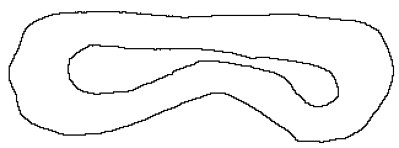
\includegraphics[interpolate=true,width=3.990000in,height=1.480000in]{contents/chapt6/figs/steer/path_method_comparison-img1.png}}%
\end{pgfscope}%
\begin{pgfscope}%
\pgfpathrectangle{\pgfqpoint{0.507645in}{0.900000in}}{\pgfqpoint{3.984710in}{1.471277in}}%
\pgfusepath{clip}%
\pgfsetbuttcap%
\pgfsetroundjoin%
\pgfsetlinewidth{1.505625pt}%
\definecolor{currentstroke}{rgb}{0.501961,0.501961,0.501961}%
\pgfsetstrokecolor{currentstroke}%
\pgfsetdash{{5.550000pt}{2.400000pt}}{0.000000pt}%
\pgfpathmoveto{\pgfqpoint{2.713490in}{1.602767in}}%
\pgfpathlineto{\pgfqpoint{2.833266in}{1.576496in}}%
\pgfpathlineto{\pgfqpoint{2.904569in}{1.558367in}}%
\pgfpathlineto{\pgfqpoint{2.951689in}{1.544537in}}%
\pgfpathlineto{\pgfqpoint{2.998361in}{1.528944in}}%
\pgfpathlineto{\pgfqpoint{3.044415in}{1.511505in}}%
\pgfpathlineto{\pgfqpoint{3.089668in}{1.492194in}}%
\pgfpathlineto{\pgfqpoint{3.133935in}{1.470986in}}%
\pgfpathlineto{\pgfqpoint{3.177033in}{1.447855in}}%
\pgfpathlineto{\pgfqpoint{3.218821in}{1.422770in}}%
\pgfpathlineto{\pgfqpoint{3.259341in}{1.395685in}}%
\pgfpathlineto{\pgfqpoint{3.298677in}{1.366550in}}%
\pgfpathlineto{\pgfqpoint{3.336912in}{1.335314in}}%
\pgfpathlineto{\pgfqpoint{3.374130in}{1.301925in}}%
\pgfpathlineto{\pgfqpoint{3.465675in}{1.215025in}}%
\pgfpathlineto{\pgfqpoint{3.484649in}{1.199210in}}%
\pgfpathlineto{\pgfqpoint{3.504129in}{1.184591in}}%
\pgfpathlineto{\pgfqpoint{3.524240in}{1.171456in}}%
\pgfpathlineto{\pgfqpoint{3.545103in}{1.160094in}}%
\pgfpathlineto{\pgfqpoint{3.566842in}{1.150794in}}%
\pgfpathlineto{\pgfqpoint{3.589511in}{1.143738in}}%
\pgfpathlineto{\pgfqpoint{3.612992in}{1.138829in}}%
\pgfpathlineto{\pgfqpoint{3.637136in}{1.135926in}}%
\pgfpathlineto{\pgfqpoint{3.661796in}{1.134885in}}%
\pgfpathlineto{\pgfqpoint{3.686824in}{1.135567in}}%
\pgfpathlineto{\pgfqpoint{3.712072in}{1.137828in}}%
\pgfpathlineto{\pgfqpoint{3.737392in}{1.141526in}}%
\pgfpathlineto{\pgfqpoint{3.762637in}{1.146520in}}%
\pgfpathlineto{\pgfqpoint{3.812310in}{1.159829in}}%
\pgfpathlineto{\pgfqpoint{3.860079in}{1.176927in}}%
\pgfpathlineto{\pgfqpoint{3.883077in}{1.186899in}}%
\pgfpathlineto{\pgfqpoint{3.905408in}{1.197851in}}%
\pgfpathlineto{\pgfqpoint{3.927016in}{1.209807in}}%
\pgfpathlineto{\pgfqpoint{3.947844in}{1.222789in}}%
\pgfpathlineto{\pgfqpoint{3.967836in}{1.236822in}}%
\pgfpathlineto{\pgfqpoint{3.986935in}{1.251928in}}%
\pgfpathlineto{\pgfqpoint{4.005084in}{1.268130in}}%
\pgfpathlineto{\pgfqpoint{4.022227in}{1.285452in}}%
\pgfpathlineto{\pgfqpoint{4.038322in}{1.303865in}}%
\pgfpathlineto{\pgfqpoint{4.053342in}{1.323293in}}%
\pgfpathlineto{\pgfqpoint{4.067260in}{1.343652in}}%
\pgfpathlineto{\pgfqpoint{4.080051in}{1.364860in}}%
\pgfpathlineto{\pgfqpoint{4.091687in}{1.386835in}}%
\pgfpathlineto{\pgfqpoint{4.102143in}{1.409496in}}%
\pgfpathlineto{\pgfqpoint{4.111393in}{1.432760in}}%
\pgfpathlineto{\pgfqpoint{4.119410in}{1.456545in}}%
\pgfpathlineto{\pgfqpoint{4.126168in}{1.480769in}}%
\pgfpathlineto{\pgfqpoint{4.131640in}{1.505349in}}%
\pgfpathlineto{\pgfqpoint{4.135785in}{1.530193in}}%
\pgfpathlineto{\pgfqpoint{4.138545in}{1.555196in}}%
\pgfpathlineto{\pgfqpoint{4.139864in}{1.580253in}}%
\pgfpathlineto{\pgfqpoint{4.139685in}{1.605258in}}%
\pgfpathlineto{\pgfqpoint{4.137948in}{1.630108in}}%
\pgfpathlineto{\pgfqpoint{4.134598in}{1.654697in}}%
\pgfpathlineto{\pgfqpoint{4.129576in}{1.678920in}}%
\pgfpathlineto{\pgfqpoint{4.122825in}{1.702673in}}%
\pgfpathlineto{\pgfqpoint{4.114287in}{1.725849in}}%
\pgfpathlineto{\pgfqpoint{4.103916in}{1.748346in}}%
\pgfpathlineto{\pgfqpoint{4.091774in}{1.770063in}}%
\pgfpathlineto{\pgfqpoint{4.077991in}{1.790905in}}%
\pgfpathlineto{\pgfqpoint{4.062697in}{1.810776in}}%
\pgfpathlineto{\pgfqpoint{4.046021in}{1.829580in}}%
\pgfpathlineto{\pgfqpoint{4.028094in}{1.847221in}}%
\pgfpathlineto{\pgfqpoint{4.009046in}{1.863604in}}%
\pgfpathlineto{\pgfqpoint{3.989005in}{1.878632in}}%
\pgfpathlineto{\pgfqpoint{3.968103in}{1.892209in}}%
\pgfpathlineto{\pgfqpoint{3.946469in}{1.904241in}}%
\pgfpathlineto{\pgfqpoint{3.924226in}{1.914664in}}%
\pgfpathlineto{\pgfqpoint{3.901454in}{1.923600in}}%
\pgfpathlineto{\pgfqpoint{3.878224in}{1.931229in}}%
\pgfpathlineto{\pgfqpoint{3.830658in}{1.943283in}}%
\pgfpathlineto{\pgfqpoint{3.782075in}{1.952266in}}%
\pgfpathlineto{\pgfqpoint{3.562641in}{1.985266in}}%
\pgfpathlineto{\pgfqpoint{3.489968in}{1.994902in}}%
\pgfpathlineto{\pgfqpoint{3.416947in}{2.001830in}}%
\pgfpathlineto{\pgfqpoint{3.343520in}{2.005879in}}%
\pgfpathlineto{\pgfqpoint{3.269854in}{2.007644in}}%
\pgfpathlineto{\pgfqpoint{3.171551in}{2.007544in}}%
\pgfpathlineto{\pgfqpoint{3.048883in}{2.007310in}}%
\pgfpathlineto{\pgfqpoint{2.975486in}{2.009845in}}%
\pgfpathlineto{\pgfqpoint{2.902278in}{2.015779in}}%
\pgfpathlineto{\pgfqpoint{2.804815in}{2.027102in}}%
\pgfpathlineto{\pgfqpoint{2.682867in}{2.041579in}}%
\pgfpathlineto{\pgfqpoint{2.609539in}{2.048320in}}%
\pgfpathlineto{\pgfqpoint{2.536124in}{2.052829in}}%
\pgfpathlineto{\pgfqpoint{2.462659in}{2.054544in}}%
\pgfpathlineto{\pgfqpoint{2.389161in}{2.053575in}}%
\pgfpathlineto{\pgfqpoint{2.119261in}{2.045800in}}%
\pgfpathlineto{\pgfqpoint{2.045723in}{2.047397in}}%
\pgfpathlineto{\pgfqpoint{1.996812in}{2.050324in}}%
\pgfpathlineto{\pgfqpoint{1.923648in}{2.057628in}}%
\pgfpathlineto{\pgfqpoint{1.777444in}{2.074555in}}%
\pgfpathlineto{\pgfqpoint{1.728547in}{2.078235in}}%
\pgfpathlineto{\pgfqpoint{1.655000in}{2.080744in}}%
\pgfpathlineto{\pgfqpoint{1.581361in}{2.080494in}}%
\pgfpathlineto{\pgfqpoint{1.483333in}{2.077570in}}%
\pgfpathlineto{\pgfqpoint{1.410038in}{2.073698in}}%
\pgfpathlineto{\pgfqpoint{1.361234in}{2.069571in}}%
\pgfpathlineto{\pgfqpoint{1.312435in}{2.063655in}}%
\pgfpathlineto{\pgfqpoint{1.263609in}{2.055473in}}%
\pgfpathlineto{\pgfqpoint{1.214939in}{2.044502in}}%
\pgfpathlineto{\pgfqpoint{1.167199in}{2.030086in}}%
\pgfpathlineto{\pgfqpoint{1.143949in}{2.021374in}}%
\pgfpathlineto{\pgfqpoint{1.121257in}{2.011548in}}%
\pgfpathlineto{\pgfqpoint{1.099233in}{2.000522in}}%
\pgfpathlineto{\pgfqpoint{1.077985in}{1.988212in}}%
\pgfpathlineto{\pgfqpoint{1.057622in}{1.974532in}}%
\pgfpathlineto{\pgfqpoint{1.038252in}{1.959401in}}%
\pgfpathlineto{\pgfqpoint{1.019967in}{1.942806in}}%
\pgfpathlineto{\pgfqpoint{1.002829in}{1.924863in}}%
\pgfpathlineto{\pgfqpoint{0.986896in}{1.905698in}}%
\pgfpathlineto{\pgfqpoint{0.972228in}{1.885437in}}%
\pgfpathlineto{\pgfqpoint{0.958885in}{1.864207in}}%
\pgfpathlineto{\pgfqpoint{0.946925in}{1.842134in}}%
\pgfpathlineto{\pgfqpoint{0.936408in}{1.819344in}}%
\pgfpathlineto{\pgfqpoint{0.927393in}{1.795964in}}%
\pgfpathlineto{\pgfqpoint{0.919939in}{1.772120in}}%
\pgfpathlineto{\pgfqpoint{0.914104in}{1.747938in}}%
\pgfpathlineto{\pgfqpoint{0.909907in}{1.723519in}}%
\pgfpathlineto{\pgfqpoint{0.907312in}{1.698929in}}%
\pgfpathlineto{\pgfqpoint{0.906280in}{1.674234in}}%
\pgfpathlineto{\pgfqpoint{0.906775in}{1.649498in}}%
\pgfpathlineto{\pgfqpoint{0.908756in}{1.624788in}}%
\pgfpathlineto{\pgfqpoint{0.912186in}{1.600168in}}%
\pgfpathlineto{\pgfqpoint{0.917026in}{1.575703in}}%
\pgfpathlineto{\pgfqpoint{0.923238in}{1.551458in}}%
\pgfpathlineto{\pgfqpoint{0.930784in}{1.527499in}}%
\pgfpathlineto{\pgfqpoint{0.939626in}{1.503892in}}%
\pgfpathlineto{\pgfqpoint{0.949733in}{1.480743in}}%
\pgfpathlineto{\pgfqpoint{0.961080in}{1.458181in}}%
\pgfpathlineto{\pgfqpoint{0.973645in}{1.436337in}}%
\pgfpathlineto{\pgfqpoint{0.987402in}{1.415344in}}%
\pgfpathlineto{\pgfqpoint{1.002326in}{1.395332in}}%
\pgfpathlineto{\pgfqpoint{1.018395in}{1.376432in}}%
\pgfpathlineto{\pgfqpoint{1.035583in}{1.358776in}}%
\pgfpathlineto{\pgfqpoint{1.053865in}{1.342495in}}%
\pgfpathlineto{\pgfqpoint{1.073219in}{1.327721in}}%
\pgfpathlineto{\pgfqpoint{1.093610in}{1.314561in}}%
\pgfpathlineto{\pgfqpoint{1.114951in}{1.302964in}}%
\pgfpathlineto{\pgfqpoint{1.137128in}{1.292814in}}%
\pgfpathlineto{\pgfqpoint{1.160029in}{1.283994in}}%
\pgfpathlineto{\pgfqpoint{1.183542in}{1.276385in}}%
\pgfpathlineto{\pgfqpoint{1.231951in}{1.264332in}}%
\pgfpathlineto{\pgfqpoint{1.281453in}{1.255715in}}%
\pgfpathlineto{\pgfqpoint{1.331164in}{1.249614in}}%
\pgfpathlineto{\pgfqpoint{1.380610in}{1.245608in}}%
\pgfpathlineto{\pgfqpoint{1.429779in}{1.243832in}}%
\pgfpathlineto{\pgfqpoint{1.478682in}{1.244450in}}%
\pgfpathlineto{\pgfqpoint{1.527328in}{1.247625in}}%
\pgfpathlineto{\pgfqpoint{1.575727in}{1.253507in}}%
\pgfpathlineto{\pgfqpoint{1.623889in}{1.261932in}}%
\pgfpathlineto{\pgfqpoint{1.671818in}{1.272435in}}%
\pgfpathlineto{\pgfqpoint{1.743291in}{1.291034in}}%
\pgfpathlineto{\pgfqpoint{1.837821in}{1.318743in}}%
\pgfpathlineto{\pgfqpoint{1.908027in}{1.341038in}}%
\pgfpathlineto{\pgfqpoint{1.977428in}{1.365171in}}%
\pgfpathlineto{\pgfqpoint{2.045833in}{1.391671in}}%
\pgfpathlineto{\pgfqpoint{2.113286in}{1.420587in}}%
\pgfpathlineto{\pgfqpoint{2.202373in}{1.461835in}}%
\pgfpathlineto{\pgfqpoint{2.336136in}{1.525357in}}%
\pgfpathlineto{\pgfqpoint{2.381384in}{1.544615in}}%
\pgfpathlineto{\pgfqpoint{2.427265in}{1.561541in}}%
\pgfpathlineto{\pgfqpoint{2.473961in}{1.575304in}}%
\pgfpathlineto{\pgfqpoint{2.521575in}{1.585414in}}%
\pgfpathlineto{\pgfqpoint{2.569956in}{1.592455in}}%
\pgfpathlineto{\pgfqpoint{2.618907in}{1.597222in}}%
\pgfpathlineto{\pgfqpoint{2.692966in}{1.601843in}}%
\pgfpathlineto{\pgfqpoint{2.692966in}{1.601843in}}%
\pgfusepath{stroke}%
\end{pgfscope}%
\begin{pgfscope}%
\pgfpathrectangle{\pgfqpoint{0.507645in}{0.900000in}}{\pgfqpoint{3.984710in}{1.471277in}}%
\pgfusepath{clip}%
\pgfsetrectcap%
\pgfsetroundjoin%
\pgfsetlinewidth{1.505625pt}%
\definecolor{currentstroke}{rgb}{0.121569,0.466667,0.705882}%
\pgfsetstrokecolor{currentstroke}%
\pgfsetdash{}{0pt}%
\pgfpathmoveto{\pgfqpoint{2.959774in}{2.003458in}}%
\pgfpathlineto{\pgfqpoint{2.885182in}{2.004370in}}%
\pgfpathlineto{\pgfqpoint{2.825045in}{2.007640in}}%
\pgfpathlineto{\pgfqpoint{2.768688in}{2.012878in}}%
\pgfpathlineto{\pgfqpoint{2.695914in}{2.022369in}}%
\pgfpathlineto{\pgfqpoint{2.537477in}{2.044177in}}%
\pgfpathlineto{\pgfqpoint{2.476269in}{2.050269in}}%
\pgfpathlineto{\pgfqpoint{2.414877in}{2.054094in}}%
\pgfpathlineto{\pgfqpoint{2.353387in}{2.055646in}}%
\pgfpathlineto{\pgfqpoint{2.279577in}{2.054935in}}%
\pgfpathlineto{\pgfqpoint{2.095099in}{2.050507in}}%
\pgfpathlineto{\pgfqpoint{2.033600in}{2.051731in}}%
\pgfpathlineto{\pgfqpoint{1.959894in}{2.055716in}}%
\pgfpathlineto{\pgfqpoint{1.812553in}{2.064863in}}%
\pgfpathlineto{\pgfqpoint{1.763353in}{2.065777in}}%
\pgfpathlineto{\pgfqpoint{1.714155in}{2.064762in}}%
\pgfpathlineto{\pgfqpoint{1.665043in}{2.061707in}}%
\pgfpathlineto{\pgfqpoint{1.616110in}{2.056514in}}%
\pgfpathlineto{\pgfqpoint{1.567448in}{2.049207in}}%
\pgfpathlineto{\pgfqpoint{1.519124in}{2.039918in}}%
\pgfpathlineto{\pgfqpoint{1.447189in}{2.023373in}}%
\pgfpathlineto{\pgfqpoint{1.375818in}{2.004539in}}%
\pgfpathlineto{\pgfqpoint{1.316810in}{1.987170in}}%
\pgfpathlineto{\pgfqpoint{1.258476in}{1.967661in}}%
\pgfpathlineto{\pgfqpoint{1.212581in}{1.949916in}}%
\pgfpathlineto{\pgfqpoint{1.178895in}{1.934842in}}%
\pgfpathlineto{\pgfqpoint{1.146137in}{1.917850in}}%
\pgfpathlineto{\pgfqpoint{1.114647in}{1.898614in}}%
\pgfpathlineto{\pgfqpoint{1.084852in}{1.876850in}}%
\pgfpathlineto{\pgfqpoint{1.066162in}{1.860851in}}%
\pgfpathlineto{\pgfqpoint{1.048516in}{1.843708in}}%
\pgfpathlineto{\pgfqpoint{1.032054in}{1.825425in}}%
\pgfpathlineto{\pgfqpoint{1.016963in}{1.805997in}}%
\pgfpathlineto{\pgfqpoint{1.003358in}{1.785500in}}%
\pgfpathlineto{\pgfqpoint{0.991389in}{1.764007in}}%
\pgfpathlineto{\pgfqpoint{0.981195in}{1.741618in}}%
\pgfpathlineto{\pgfqpoint{0.972879in}{1.718467in}}%
\pgfpathlineto{\pgfqpoint{0.966538in}{1.694698in}}%
\pgfpathlineto{\pgfqpoint{0.962256in}{1.670474in}}%
\pgfpathlineto{\pgfqpoint{0.960099in}{1.645970in}}%
\pgfpathlineto{\pgfqpoint{0.960072in}{1.621369in}}%
\pgfpathlineto{\pgfqpoint{0.962053in}{1.596849in}}%
\pgfpathlineto{\pgfqpoint{0.965938in}{1.572557in}}%
\pgfpathlineto{\pgfqpoint{0.971694in}{1.548639in}}%
\pgfpathlineto{\pgfqpoint{0.979241in}{1.525224in}}%
\pgfpathlineto{\pgfqpoint{0.988482in}{1.502424in}}%
\pgfpathlineto{\pgfqpoint{0.999382in}{1.480369in}}%
\pgfpathlineto{\pgfqpoint{1.011865in}{1.459171in}}%
\pgfpathlineto{\pgfqpoint{1.025862in}{1.438939in}}%
\pgfpathlineto{\pgfqpoint{1.041342in}{1.419818in}}%
\pgfpathlineto{\pgfqpoint{1.058132in}{1.401837in}}%
\pgfpathlineto{\pgfqpoint{1.076143in}{1.385077in}}%
\pgfpathlineto{\pgfqpoint{1.095293in}{1.369634in}}%
\pgfpathlineto{\pgfqpoint{1.115489in}{1.355584in}}%
\pgfpathlineto{\pgfqpoint{1.136624in}{1.342993in}}%
\pgfpathlineto{\pgfqpoint{1.158592in}{1.331916in}}%
\pgfpathlineto{\pgfqpoint{1.181278in}{1.322399in}}%
\pgfpathlineto{\pgfqpoint{1.204571in}{1.314481in}}%
\pgfpathlineto{\pgfqpoint{1.228337in}{1.308120in}}%
\pgfpathlineto{\pgfqpoint{1.264622in}{1.301430in}}%
\pgfpathlineto{\pgfqpoint{1.301336in}{1.297721in}}%
\pgfpathlineto{\pgfqpoint{1.338223in}{1.296656in}}%
\pgfpathlineto{\pgfqpoint{1.375104in}{1.297941in}}%
\pgfpathlineto{\pgfqpoint{1.411858in}{1.301271in}}%
\pgfpathlineto{\pgfqpoint{1.460546in}{1.308384in}}%
\pgfpathlineto{\pgfqpoint{1.508789in}{1.318074in}}%
\pgfpathlineto{\pgfqpoint{1.568587in}{1.332488in}}%
\pgfpathlineto{\pgfqpoint{1.651676in}{1.355123in}}%
\pgfpathlineto{\pgfqpoint{1.805799in}{1.397820in}}%
\pgfpathlineto{\pgfqpoint{1.853778in}{1.408751in}}%
\pgfpathlineto{\pgfqpoint{1.902169in}{1.417677in}}%
\pgfpathlineto{\pgfqpoint{1.950908in}{1.424447in}}%
\pgfpathlineto{\pgfqpoint{1.999901in}{1.429044in}}%
\pgfpathlineto{\pgfqpoint{2.098128in}{1.435220in}}%
\pgfpathlineto{\pgfqpoint{2.184030in}{1.441290in}}%
\pgfpathlineto{\pgfqpoint{2.257439in}{1.449002in}}%
\pgfpathlineto{\pgfqpoint{2.330589in}{1.458886in}}%
\pgfpathlineto{\pgfqpoint{2.513241in}{1.485159in}}%
\pgfpathlineto{\pgfqpoint{2.574480in}{1.490910in}}%
\pgfpathlineto{\pgfqpoint{2.623633in}{1.493209in}}%
\pgfpathlineto{\pgfqpoint{2.672837in}{1.492929in}}%
\pgfpathlineto{\pgfqpoint{2.709683in}{1.490832in}}%
\pgfpathlineto{\pgfqpoint{2.746386in}{1.486980in}}%
\pgfpathlineto{\pgfqpoint{2.782854in}{1.481321in}}%
\pgfpathlineto{\pgfqpoint{2.818991in}{1.473830in}}%
\pgfpathlineto{\pgfqpoint{2.854726in}{1.464608in}}%
\pgfpathlineto{\pgfqpoint{2.901657in}{1.449825in}}%
\pgfpathlineto{\pgfqpoint{2.947722in}{1.432524in}}%
\pgfpathlineto{\pgfqpoint{3.004327in}{1.408452in}}%
\pgfpathlineto{\pgfqpoint{3.150044in}{1.342530in}}%
\pgfpathlineto{\pgfqpoint{3.284984in}{1.282641in}}%
\pgfpathlineto{\pgfqpoint{3.464940in}{1.204142in}}%
\pgfpathlineto{\pgfqpoint{3.510425in}{1.187238in}}%
\pgfpathlineto{\pgfqpoint{3.545059in}{1.176691in}}%
\pgfpathlineto{\pgfqpoint{3.580167in}{1.168543in}}%
\pgfpathlineto{\pgfqpoint{3.615670in}{1.163385in}}%
\pgfpathlineto{\pgfqpoint{3.652239in}{1.161480in}}%
\pgfpathlineto{\pgfqpoint{3.688995in}{1.162719in}}%
\pgfpathlineto{\pgfqpoint{3.725503in}{1.167166in}}%
\pgfpathlineto{\pgfqpoint{3.761476in}{1.174814in}}%
\pgfpathlineto{\pgfqpoint{3.796621in}{1.185647in}}%
\pgfpathlineto{\pgfqpoint{3.830659in}{1.199574in}}%
\pgfpathlineto{\pgfqpoint{3.863306in}{1.216507in}}%
\pgfpathlineto{\pgfqpoint{3.894368in}{1.236200in}}%
\pgfpathlineto{\pgfqpoint{3.923729in}{1.258350in}}%
\pgfpathlineto{\pgfqpoint{3.951146in}{1.282865in}}%
\pgfpathlineto{\pgfqpoint{3.976383in}{1.309617in}}%
\pgfpathlineto{\pgfqpoint{3.999256in}{1.338417in}}%
\pgfpathlineto{\pgfqpoint{4.019480in}{1.369133in}}%
\pgfpathlineto{\pgfqpoint{4.036857in}{1.401547in}}%
\pgfpathlineto{\pgfqpoint{4.051481in}{1.435293in}}%
\pgfpathlineto{\pgfqpoint{4.063169in}{1.470164in}}%
\pgfpathlineto{\pgfqpoint{4.071733in}{1.505931in}}%
\pgfpathlineto{\pgfqpoint{4.075695in}{1.530131in}}%
\pgfpathlineto{\pgfqpoint{4.078130in}{1.554532in}}%
\pgfpathlineto{\pgfqpoint{4.078998in}{1.579038in}}%
\pgfpathlineto{\pgfqpoint{4.078274in}{1.603549in}}%
\pgfpathlineto{\pgfqpoint{4.075850in}{1.627951in}}%
\pgfpathlineto{\pgfqpoint{4.071816in}{1.652139in}}%
\pgfpathlineto{\pgfqpoint{4.066281in}{1.676028in}}%
\pgfpathlineto{\pgfqpoint{4.059223in}{1.699512in}}%
\pgfpathlineto{\pgfqpoint{4.050639in}{1.722483in}}%
\pgfpathlineto{\pgfqpoint{4.040587in}{1.744849in}}%
\pgfpathlineto{\pgfqpoint{4.029058in}{1.766493in}}%
\pgfpathlineto{\pgfqpoint{4.016126in}{1.787327in}}%
\pgfpathlineto{\pgfqpoint{4.001819in}{1.807242in}}%
\pgfpathlineto{\pgfqpoint{3.986176in}{1.826126in}}%
\pgfpathlineto{\pgfqpoint{3.969264in}{1.843883in}}%
\pgfpathlineto{\pgfqpoint{3.951177in}{1.860440in}}%
\pgfpathlineto{\pgfqpoint{3.922190in}{1.883074in}}%
\pgfpathlineto{\pgfqpoint{3.891301in}{1.903037in}}%
\pgfpathlineto{\pgfqpoint{3.858862in}{1.920370in}}%
\pgfpathlineto{\pgfqpoint{3.825183in}{1.935152in}}%
\pgfpathlineto{\pgfqpoint{3.790544in}{1.947524in}}%
\pgfpathlineto{\pgfqpoint{3.755205in}{1.957731in}}%
\pgfpathlineto{\pgfqpoint{3.707351in}{1.968469in}}%
\pgfpathlineto{\pgfqpoint{3.659047in}{1.976978in}}%
\pgfpathlineto{\pgfqpoint{3.598329in}{1.985482in}}%
\pgfpathlineto{\pgfqpoint{3.500863in}{1.996601in}}%
\pgfpathlineto{\pgfqpoint{3.403157in}{2.005367in}}%
\pgfpathlineto{\pgfqpoint{3.329726in}{2.009953in}}%
\pgfpathlineto{\pgfqpoint{3.256193in}{2.012346in}}%
\pgfpathlineto{\pgfqpoint{3.170358in}{2.012638in}}%
\pgfpathlineto{\pgfqpoint{3.047758in}{2.010146in}}%
\pgfpathlineto{\pgfqpoint{3.047758in}{2.010146in}}%
\pgfusepath{stroke}%
\end{pgfscope}%
\begin{pgfscope}%
\pgfpathrectangle{\pgfqpoint{0.507645in}{0.900000in}}{\pgfqpoint{3.984710in}{1.471277in}}%
\pgfusepath{clip}%
\pgfsetbuttcap%
\pgfsetroundjoin%
\pgfsetlinewidth{1.505625pt}%
\definecolor{currentstroke}{rgb}{1.000000,0.000000,0.000000}%
\pgfsetstrokecolor{currentstroke}%
\pgfsetstrokeopacity{0.500000}%
\pgfsetdash{{9.600000pt}{2.400000pt}{1.500000pt}{2.400000pt}}{0.000000pt}%
\pgfpathmoveto{\pgfqpoint{2.950186in}{1.999667in}}%
\pgfpathlineto{\pgfqpoint{2.935056in}{1.999875in}}%
\pgfpathlineto{\pgfqpoint{2.919950in}{2.000467in}}%
\pgfpathlineto{\pgfqpoint{2.904875in}{2.001420in}}%
\pgfpathlineto{\pgfqpoint{2.889836in}{2.002708in}}%
\pgfpathlineto{\pgfqpoint{2.874834in}{2.004309in}}%
\pgfpathlineto{\pgfqpoint{2.859873in}{2.006199in}}%
\pgfpathlineto{\pgfqpoint{2.844952in}{2.008353in}}%
\pgfpathlineto{\pgfqpoint{2.830070in}{2.010749in}}%
\pgfpathlineto{\pgfqpoint{2.815226in}{2.013363in}}%
\pgfpathlineto{\pgfqpoint{2.800416in}{2.016173in}}%
\pgfpathlineto{\pgfqpoint{2.785636in}{2.019156in}}%
\pgfpathlineto{\pgfqpoint{2.770881in}{2.022288in}}%
\pgfpathlineto{\pgfqpoint{2.756145in}{2.025547in}}%
\pgfpathlineto{\pgfqpoint{2.741421in}{2.028911in}}%
\pgfpathlineto{\pgfqpoint{2.726703in}{2.032357in}}%
\pgfpathlineto{\pgfqpoint{2.711982in}{2.035866in}}%
\pgfpathlineto{\pgfqpoint{2.697253in}{2.039424in}}%
\pgfpathlineto{\pgfqpoint{2.682513in}{2.043015in}}%
\pgfpathlineto{\pgfqpoint{2.667758in}{2.046625in}}%
\pgfpathlineto{\pgfqpoint{2.652983in}{2.050240in}}%
\pgfpathlineto{\pgfqpoint{2.638185in}{2.053845in}}%
\pgfpathlineto{\pgfqpoint{2.623361in}{2.057426in}}%
\pgfpathlineto{\pgfqpoint{2.608506in}{2.060967in}}%
\pgfpathlineto{\pgfqpoint{2.593616in}{2.064454in}}%
\pgfpathlineto{\pgfqpoint{2.578689in}{2.067873in}}%
\pgfpathlineto{\pgfqpoint{2.563722in}{2.071207in}}%
\pgfpathlineto{\pgfqpoint{2.548711in}{2.074442in}}%
\pgfpathlineto{\pgfqpoint{2.533653in}{2.077563in}}%
\pgfpathlineto{\pgfqpoint{2.518547in}{2.080555in}}%
\pgfpathlineto{\pgfqpoint{2.503390in}{2.083402in}}%
\pgfpathlineto{\pgfqpoint{2.488181in}{2.086089in}}%
\pgfpathlineto{\pgfqpoint{2.472935in}{2.088602in}}%
\pgfpathlineto{\pgfqpoint{2.457674in}{2.090940in}}%
\pgfpathlineto{\pgfqpoint{2.442403in}{2.093103in}}%
\pgfpathlineto{\pgfqpoint{2.427129in}{2.095091in}}%
\pgfpathlineto{\pgfqpoint{2.411856in}{2.096906in}}%
\pgfpathlineto{\pgfqpoint{2.396591in}{2.098548in}}%
\pgfpathlineto{\pgfqpoint{2.381340in}{2.100018in}}%
\pgfpathlineto{\pgfqpoint{2.366108in}{2.101317in}}%
\pgfpathlineto{\pgfqpoint{2.350900in}{2.102446in}}%
\pgfpathlineto{\pgfqpoint{2.335720in}{2.103406in}}%
\pgfpathlineto{\pgfqpoint{2.320573in}{2.104197in}}%
\pgfpathlineto{\pgfqpoint{2.305462in}{2.104821in}}%
\pgfpathlineto{\pgfqpoint{2.290391in}{2.105278in}}%
\pgfpathlineto{\pgfqpoint{2.275362in}{2.105568in}}%
\pgfpathlineto{\pgfqpoint{2.260377in}{2.105692in}}%
\pgfpathlineto{\pgfqpoint{2.245438in}{2.105651in}}%
\pgfpathlineto{\pgfqpoint{2.230541in}{2.105444in}}%
\pgfpathlineto{\pgfqpoint{2.215682in}{2.105070in}}%
\pgfpathlineto{\pgfqpoint{2.215682in}{2.105070in}}%
\pgfpathlineto{\pgfqpoint{2.205796in}{2.104777in}}%
\pgfpathlineto{\pgfqpoint{2.195922in}{2.104508in}}%
\pgfpathlineto{\pgfqpoint{2.186063in}{2.104266in}}%
\pgfpathlineto{\pgfqpoint{2.176218in}{2.104053in}}%
\pgfpathlineto{\pgfqpoint{2.166387in}{2.103873in}}%
\pgfpathlineto{\pgfqpoint{2.156571in}{2.103726in}}%
\pgfpathlineto{\pgfqpoint{2.146770in}{2.103615in}}%
\pgfpathlineto{\pgfqpoint{2.136984in}{2.103543in}}%
\pgfpathlineto{\pgfqpoint{2.127214in}{2.103512in}}%
\pgfpathlineto{\pgfqpoint{2.117460in}{2.103524in}}%
\pgfpathlineto{\pgfqpoint{2.107722in}{2.103581in}}%
\pgfpathlineto{\pgfqpoint{2.098001in}{2.103685in}}%
\pgfpathlineto{\pgfqpoint{2.088296in}{2.103840in}}%
\pgfpathlineto{\pgfqpoint{2.078609in}{2.104046in}}%
\pgfpathlineto{\pgfqpoint{2.068939in}{2.104307in}}%
\pgfpathlineto{\pgfqpoint{2.059286in}{2.104624in}}%
\pgfpathlineto{\pgfqpoint{2.049651in}{2.104999in}}%
\pgfpathlineto{\pgfqpoint{2.040035in}{2.105436in}}%
\pgfpathlineto{\pgfqpoint{2.030437in}{2.105935in}}%
\pgfpathlineto{\pgfqpoint{2.020857in}{2.106499in}}%
\pgfpathlineto{\pgfqpoint{2.011296in}{2.107130in}}%
\pgfpathlineto{\pgfqpoint{2.001754in}{2.107831in}}%
\pgfpathlineto{\pgfqpoint{1.992204in}{2.108604in}}%
\pgfpathlineto{\pgfqpoint{1.982623in}{2.109446in}}%
\pgfpathlineto{\pgfqpoint{1.973010in}{2.110353in}}%
\pgfpathlineto{\pgfqpoint{1.963364in}{2.111317in}}%
\pgfpathlineto{\pgfqpoint{1.953687in}{2.112335in}}%
\pgfpathlineto{\pgfqpoint{1.943976in}{2.113399in}}%
\pgfpathlineto{\pgfqpoint{1.934233in}{2.114505in}}%
\pgfpathlineto{\pgfqpoint{1.924455in}{2.115647in}}%
\pgfpathlineto{\pgfqpoint{1.914644in}{2.116818in}}%
\pgfpathlineto{\pgfqpoint{1.904798in}{2.118012in}}%
\pgfpathlineto{\pgfqpoint{1.894917in}{2.119225in}}%
\pgfpathlineto{\pgfqpoint{1.885001in}{2.120448in}}%
\pgfpathlineto{\pgfqpoint{1.875049in}{2.121678in}}%
\pgfpathlineto{\pgfqpoint{1.865061in}{2.122906in}}%
\pgfpathlineto{\pgfqpoint{1.855036in}{2.124127in}}%
\pgfpathlineto{\pgfqpoint{1.844974in}{2.125335in}}%
\pgfpathlineto{\pgfqpoint{1.834874in}{2.126522in}}%
\pgfpathlineto{\pgfqpoint{1.824736in}{2.127683in}}%
\pgfpathlineto{\pgfqpoint{1.814559in}{2.128812in}}%
\pgfpathlineto{\pgfqpoint{1.804343in}{2.129900in}}%
\pgfpathlineto{\pgfqpoint{1.794087in}{2.130943in}}%
\pgfpathlineto{\pgfqpoint{1.783791in}{2.131932in}}%
\pgfpathlineto{\pgfqpoint{1.773453in}{2.132861in}}%
\pgfpathlineto{\pgfqpoint{1.763075in}{2.133724in}}%
\pgfpathlineto{\pgfqpoint{1.752663in}{2.134512in}}%
\pgfpathlineto{\pgfqpoint{1.742256in}{2.135223in}}%
\pgfpathlineto{\pgfqpoint{1.731858in}{2.135857in}}%
\pgfusepath{stroke}%
\end{pgfscope}%
\begin{pgfscope}%
\pgfpathrectangle{\pgfqpoint{0.507645in}{0.900000in}}{\pgfqpoint{3.984710in}{1.471277in}}%
\pgfusepath{clip}%
\pgfsetrectcap%
\pgfsetroundjoin%
\pgfsetlinewidth{1.505625pt}%
\definecolor{currentstroke}{rgb}{1.000000,0.000000,0.000000}%
\pgfsetstrokecolor{currentstroke}%
\pgfsetstrokeopacity{0.500000}%
\pgfsetdash{}{0pt}%
\pgfpathmoveto{\pgfqpoint{2.950186in}{1.999667in}}%
\pgfusepath{stroke}%
\end{pgfscope}%
\begin{pgfscope}%
\pgfpathrectangle{\pgfqpoint{0.507645in}{0.900000in}}{\pgfqpoint{3.984710in}{1.471277in}}%
\pgfusepath{clip}%
\pgfsetbuttcap%
\pgfsetmiterjoin%
\definecolor{currentfill}{rgb}{1.000000,0.000000,0.000000}%
\pgfsetfillcolor{currentfill}%
\pgfsetfillopacity{0.500000}%
\pgfsetlinewidth{1.003750pt}%
\definecolor{currentstroke}{rgb}{1.000000,0.000000,0.000000}%
\pgfsetstrokecolor{currentstroke}%
\pgfsetstrokeopacity{0.500000}%
\pgfsetdash{}{0pt}%
\pgfsys@defobject{currentmarker}{\pgfqpoint{-0.041667in}{-0.041667in}}{\pgfqpoint{0.041667in}{0.041667in}}{%
\pgfpathmoveto{\pgfqpoint{-0.041667in}{-0.041667in}}%
\pgfpathlineto{\pgfqpoint{0.041667in}{-0.041667in}}%
\pgfpathlineto{\pgfqpoint{0.041667in}{0.041667in}}%
\pgfpathlineto{\pgfqpoint{-0.041667in}{0.041667in}}%
\pgfpathlineto{\pgfqpoint{-0.041667in}{-0.041667in}}%
\pgfpathclose%
\pgfusepath{stroke,fill}%
}%
\begin{pgfscope}%
\pgfsys@transformshift{2.950186in}{1.999667in}%
\pgfsys@useobject{currentmarker}{}%
\end{pgfscope}%
\end{pgfscope}%
\begin{pgfscope}%
\pgfpathrectangle{\pgfqpoint{0.507645in}{0.900000in}}{\pgfqpoint{3.984710in}{1.471277in}}%
\pgfusepath{clip}%
\pgfsetbuttcap%
\pgfsetroundjoin%
\pgfsetlinewidth{1.505625pt}%
\definecolor{currentstroke}{rgb}{1.000000,0.000000,0.000000}%
\pgfsetstrokecolor{currentstroke}%
\pgfsetstrokeopacity{0.500000}%
\pgfsetdash{{9.600000pt}{2.400000pt}{1.500000pt}{2.400000pt}}{0.000000pt}%
\pgfpathmoveto{\pgfqpoint{2.535555in}{2.039768in}}%
\pgfpathlineto{\pgfqpoint{2.520689in}{2.040926in}}%
\pgfpathlineto{\pgfqpoint{2.505816in}{2.041947in}}%
\pgfpathlineto{\pgfqpoint{2.490936in}{2.042827in}}%
\pgfpathlineto{\pgfqpoint{2.476045in}{2.043561in}}%
\pgfpathlineto{\pgfqpoint{2.461137in}{2.044155in}}%
\pgfpathlineto{\pgfqpoint{2.446214in}{2.044620in}}%
\pgfpathlineto{\pgfqpoint{2.431275in}{2.044967in}}%
\pgfpathlineto{\pgfqpoint{2.416323in}{2.045204in}}%
\pgfpathlineto{\pgfqpoint{2.401358in}{2.045343in}}%
\pgfpathlineto{\pgfqpoint{2.386381in}{2.045395in}}%
\pgfpathlineto{\pgfqpoint{2.371394in}{2.045369in}}%
\pgfpathlineto{\pgfqpoint{2.356397in}{2.045276in}}%
\pgfpathlineto{\pgfqpoint{2.341392in}{2.045127in}}%
\pgfpathlineto{\pgfqpoint{2.326378in}{2.044932in}}%
\pgfpathlineto{\pgfqpoint{2.311356in}{2.044702in}}%
\pgfpathlineto{\pgfqpoint{2.296328in}{2.044447in}}%
\pgfpathlineto{\pgfqpoint{2.281294in}{2.044178in}}%
\pgfpathlineto{\pgfqpoint{2.266254in}{2.043905in}}%
\pgfpathlineto{\pgfqpoint{2.251209in}{2.043640in}}%
\pgfpathlineto{\pgfqpoint{2.236159in}{2.043391in}}%
\pgfpathlineto{\pgfqpoint{2.221106in}{2.043170in}}%
\pgfpathlineto{\pgfqpoint{2.206051in}{2.042985in}}%
\pgfpathlineto{\pgfqpoint{2.190995in}{2.042843in}}%
\pgfpathlineto{\pgfqpoint{2.175940in}{2.042755in}}%
\pgfpathlineto{\pgfqpoint{2.160886in}{2.042727in}}%
\pgfpathlineto{\pgfqpoint{2.145835in}{2.042768in}}%
\pgfpathlineto{\pgfqpoint{2.130787in}{2.042888in}}%
\pgfpathlineto{\pgfqpoint{2.115744in}{2.043094in}}%
\pgfpathlineto{\pgfqpoint{2.100708in}{2.043394in}}%
\pgfpathlineto{\pgfqpoint{2.085678in}{2.043798in}}%
\pgfpathlineto{\pgfqpoint{2.070656in}{2.044313in}}%
\pgfpathlineto{\pgfqpoint{2.055642in}{2.044949in}}%
\pgfpathlineto{\pgfqpoint{2.040639in}{2.045713in}}%
\pgfpathlineto{\pgfqpoint{2.025646in}{2.046613in}}%
\pgfpathlineto{\pgfqpoint{2.010664in}{2.047659in}}%
\pgfpathlineto{\pgfqpoint{1.995694in}{2.048859in}}%
\pgfpathlineto{\pgfqpoint{1.980739in}{2.050214in}}%
\pgfpathlineto{\pgfqpoint{1.965798in}{2.051705in}}%
\pgfpathlineto{\pgfqpoint{1.950867in}{2.053314in}}%
\pgfpathlineto{\pgfqpoint{1.935946in}{2.055017in}}%
\pgfpathlineto{\pgfqpoint{1.921031in}{2.056796in}}%
\pgfpathlineto{\pgfqpoint{1.906122in}{2.058629in}}%
\pgfpathlineto{\pgfqpoint{1.891216in}{2.060496in}}%
\pgfpathlineto{\pgfqpoint{1.876311in}{2.062376in}}%
\pgfpathlineto{\pgfqpoint{1.861407in}{2.064247in}}%
\pgfpathlineto{\pgfqpoint{1.846500in}{2.066090in}}%
\pgfpathlineto{\pgfqpoint{1.831589in}{2.067884in}}%
\pgfpathlineto{\pgfqpoint{1.816674in}{2.069607in}}%
\pgfpathlineto{\pgfqpoint{1.801752in}{2.071240in}}%
\pgfpathlineto{\pgfqpoint{1.801752in}{2.071240in}}%
\pgfpathlineto{\pgfqpoint{1.791799in}{2.072270in}}%
\pgfpathlineto{\pgfqpoint{1.781843in}{2.073246in}}%
\pgfpathlineto{\pgfqpoint{1.771883in}{2.074164in}}%
\pgfpathlineto{\pgfqpoint{1.761918in}{2.075017in}}%
\pgfpathlineto{\pgfqpoint{1.751948in}{2.075798in}}%
\pgfpathlineto{\pgfqpoint{1.741972in}{2.076505in}}%
\pgfpathlineto{\pgfqpoint{1.731990in}{2.077139in}}%
\pgfpathlineto{\pgfqpoint{1.722003in}{2.077702in}}%
\pgfpathlineto{\pgfqpoint{1.712012in}{2.078198in}}%
\pgfpathlineto{\pgfqpoint{1.702016in}{2.078628in}}%
\pgfpathlineto{\pgfqpoint{1.692015in}{2.078996in}}%
\pgfpathlineto{\pgfqpoint{1.682012in}{2.079303in}}%
\pgfpathlineto{\pgfqpoint{1.672005in}{2.079553in}}%
\pgfpathlineto{\pgfqpoint{1.661996in}{2.079747in}}%
\pgfpathlineto{\pgfqpoint{1.651984in}{2.079889in}}%
\pgfpathlineto{\pgfqpoint{1.641971in}{2.079980in}}%
\pgfpathlineto{\pgfqpoint{1.631956in}{2.080023in}}%
\pgfpathlineto{\pgfqpoint{1.621941in}{2.080022in}}%
\pgfpathlineto{\pgfqpoint{1.611924in}{2.079977in}}%
\pgfpathlineto{\pgfqpoint{1.601908in}{2.079892in}}%
\pgfpathlineto{\pgfqpoint{1.591893in}{2.079769in}}%
\pgfpathlineto{\pgfqpoint{1.581878in}{2.079611in}}%
\pgfpathlineto{\pgfqpoint{1.571864in}{2.079420in}}%
\pgfpathlineto{\pgfqpoint{1.561852in}{2.079199in}}%
\pgfpathlineto{\pgfqpoint{1.551843in}{2.078950in}}%
\pgfpathlineto{\pgfqpoint{1.541835in}{2.078676in}}%
\pgfpathlineto{\pgfqpoint{1.531831in}{2.078379in}}%
\pgfpathlineto{\pgfqpoint{1.521831in}{2.078062in}}%
\pgfpathlineto{\pgfqpoint{1.511834in}{2.077727in}}%
\pgfpathlineto{\pgfqpoint{1.501842in}{2.077377in}}%
\pgfpathlineto{\pgfqpoint{1.491854in}{2.077009in}}%
\pgfpathlineto{\pgfqpoint{1.481871in}{2.076619in}}%
\pgfpathlineto{\pgfqpoint{1.471892in}{2.076203in}}%
\pgfpathlineto{\pgfqpoint{1.461918in}{2.075758in}}%
\pgfpathlineto{\pgfqpoint{1.451946in}{2.075279in}}%
\pgfpathlineto{\pgfqpoint{1.441978in}{2.074762in}}%
\pgfpathlineto{\pgfqpoint{1.432013in}{2.074204in}}%
\pgfpathlineto{\pgfqpoint{1.422051in}{2.073599in}}%
\pgfpathlineto{\pgfqpoint{1.412092in}{2.072945in}}%
\pgfpathlineto{\pgfqpoint{1.402134in}{2.072237in}}%
\pgfpathlineto{\pgfqpoint{1.392178in}{2.071470in}}%
\pgfpathlineto{\pgfqpoint{1.382224in}{2.070642in}}%
\pgfpathlineto{\pgfqpoint{1.372271in}{2.069748in}}%
\pgfpathlineto{\pgfqpoint{1.362319in}{2.068784in}}%
\pgfpathlineto{\pgfqpoint{1.352367in}{2.067746in}}%
\pgfpathlineto{\pgfqpoint{1.342416in}{2.066629in}}%
\pgfpathlineto{\pgfqpoint{1.332465in}{2.065431in}}%
\pgfpathlineto{\pgfqpoint{1.322514in}{2.064146in}}%
\pgfpathlineto{\pgfqpoint{1.312562in}{2.062771in}}%
\pgfusepath{stroke}%
\end{pgfscope}%
\begin{pgfscope}%
\pgfpathrectangle{\pgfqpoint{0.507645in}{0.900000in}}{\pgfqpoint{3.984710in}{1.471277in}}%
\pgfusepath{clip}%
\pgfsetrectcap%
\pgfsetroundjoin%
\pgfsetlinewidth{1.505625pt}%
\definecolor{currentstroke}{rgb}{1.000000,0.000000,0.000000}%
\pgfsetstrokecolor{currentstroke}%
\pgfsetstrokeopacity{0.500000}%
\pgfsetdash{}{0pt}%
\pgfpathmoveto{\pgfqpoint{2.535555in}{2.039768in}}%
\pgfusepath{stroke}%
\end{pgfscope}%
\begin{pgfscope}%
\pgfpathrectangle{\pgfqpoint{0.507645in}{0.900000in}}{\pgfqpoint{3.984710in}{1.471277in}}%
\pgfusepath{clip}%
\pgfsetbuttcap%
\pgfsetmiterjoin%
\definecolor{currentfill}{rgb}{1.000000,0.000000,0.000000}%
\pgfsetfillcolor{currentfill}%
\pgfsetfillopacity{0.500000}%
\pgfsetlinewidth{1.003750pt}%
\definecolor{currentstroke}{rgb}{1.000000,0.000000,0.000000}%
\pgfsetstrokecolor{currentstroke}%
\pgfsetstrokeopacity{0.500000}%
\pgfsetdash{}{0pt}%
\pgfsys@defobject{currentmarker}{\pgfqpoint{-0.041667in}{-0.041667in}}{\pgfqpoint{0.041667in}{0.041667in}}{%
\pgfpathmoveto{\pgfqpoint{-0.041667in}{-0.041667in}}%
\pgfpathlineto{\pgfqpoint{0.041667in}{-0.041667in}}%
\pgfpathlineto{\pgfqpoint{0.041667in}{0.041667in}}%
\pgfpathlineto{\pgfqpoint{-0.041667in}{0.041667in}}%
\pgfpathlineto{\pgfqpoint{-0.041667in}{-0.041667in}}%
\pgfpathclose%
\pgfusepath{stroke,fill}%
}%
\begin{pgfscope}%
\pgfsys@transformshift{2.535555in}{2.039768in}%
\pgfsys@useobject{currentmarker}{}%
\end{pgfscope}%
\end{pgfscope}%
\begin{pgfscope}%
\pgfpathrectangle{\pgfqpoint{0.507645in}{0.900000in}}{\pgfqpoint{3.984710in}{1.471277in}}%
\pgfusepath{clip}%
\pgfsetbuttcap%
\pgfsetroundjoin%
\pgfsetlinewidth{1.505625pt}%
\definecolor{currentstroke}{rgb}{1.000000,0.000000,0.000000}%
\pgfsetstrokecolor{currentstroke}%
\pgfsetstrokeopacity{0.500000}%
\pgfsetdash{{9.600000pt}{2.400000pt}{1.500000pt}{2.400000pt}}{0.000000pt}%
\pgfpathmoveto{\pgfqpoint{2.022010in}{2.061353in}}%
\pgfpathlineto{\pgfqpoint{2.007194in}{2.062516in}}%
\pgfpathlineto{\pgfqpoint{1.992378in}{2.063589in}}%
\pgfpathlineto{\pgfqpoint{1.977535in}{2.064581in}}%
\pgfpathlineto{\pgfqpoint{1.962656in}{2.065483in}}%
\pgfpathlineto{\pgfqpoint{1.947736in}{2.066285in}}%
\pgfpathlineto{\pgfqpoint{1.932773in}{2.066978in}}%
\pgfpathlineto{\pgfqpoint{1.917767in}{2.067552in}}%
\pgfpathlineto{\pgfqpoint{1.902720in}{2.067995in}}%
\pgfpathlineto{\pgfqpoint{1.887637in}{2.068298in}}%
\pgfpathlineto{\pgfqpoint{1.872521in}{2.068448in}}%
\pgfpathlineto{\pgfqpoint{1.857379in}{2.068436in}}%
\pgfpathlineto{\pgfqpoint{1.842220in}{2.068248in}}%
\pgfpathlineto{\pgfqpoint{1.827053in}{2.067874in}}%
\pgfpathlineto{\pgfqpoint{1.811888in}{2.067301in}}%
\pgfpathlineto{\pgfqpoint{1.796735in}{2.066519in}}%
\pgfpathlineto{\pgfqpoint{1.781607in}{2.065516in}}%
\pgfpathlineto{\pgfqpoint{1.766516in}{2.064280in}}%
\pgfpathlineto{\pgfqpoint{1.751475in}{2.062803in}}%
\pgfpathlineto{\pgfqpoint{1.736477in}{2.061080in}}%
\pgfpathlineto{\pgfqpoint{1.721514in}{2.059131in}}%
\pgfpathlineto{\pgfqpoint{1.706585in}{2.056974in}}%
\pgfpathlineto{\pgfqpoint{1.691688in}{2.054630in}}%
\pgfpathlineto{\pgfqpoint{1.676821in}{2.052117in}}%
\pgfpathlineto{\pgfqpoint{1.661982in}{2.049456in}}%
\pgfpathlineto{\pgfqpoint{1.647168in}{2.046664in}}%
\pgfpathlineto{\pgfqpoint{1.632375in}{2.043763in}}%
\pgfpathlineto{\pgfqpoint{1.617601in}{2.040769in}}%
\pgfpathlineto{\pgfqpoint{1.602840in}{2.037703in}}%
\pgfpathlineto{\pgfqpoint{1.588091in}{2.034583in}}%
\pgfpathlineto{\pgfqpoint{1.573347in}{2.031428in}}%
\pgfpathlineto{\pgfqpoint{1.558605in}{2.028257in}}%
\pgfpathlineto{\pgfqpoint{1.543861in}{2.025088in}}%
\pgfpathlineto{\pgfqpoint{1.529111in}{2.021939in}}%
\pgfpathlineto{\pgfqpoint{1.514351in}{2.018830in}}%
\pgfpathlineto{\pgfqpoint{1.499605in}{2.015778in}}%
\pgfpathlineto{\pgfqpoint{1.484934in}{2.012789in}}%
\pgfpathlineto{\pgfqpoint{1.470344in}{2.009861in}}%
\pgfpathlineto{\pgfqpoint{1.455839in}{2.006991in}}%
\pgfpathlineto{\pgfqpoint{1.441420in}{2.004178in}}%
\pgfpathlineto{\pgfqpoint{1.427089in}{2.001420in}}%
\pgfpathlineto{\pgfqpoint{1.412846in}{1.998716in}}%
\pgfpathlineto{\pgfqpoint{1.398689in}{1.996064in}}%
\pgfpathlineto{\pgfqpoint{1.384615in}{1.993464in}}%
\pgfpathlineto{\pgfqpoint{1.370621in}{1.990914in}}%
\pgfpathlineto{\pgfqpoint{1.356701in}{1.988414in}}%
\pgfpathlineto{\pgfqpoint{1.342845in}{1.985962in}}%
\pgfpathlineto{\pgfqpoint{1.329046in}{1.983558in}}%
\pgfpathlineto{\pgfqpoint{1.315291in}{1.981200in}}%
\pgfpathlineto{\pgfqpoint{1.301567in}{1.978886in}}%
\pgfpathlineto{\pgfqpoint{1.301567in}{1.978886in}}%
\pgfpathlineto{\pgfqpoint{1.292436in}{1.977312in}}%
\pgfpathlineto{\pgfqpoint{1.283331in}{1.975643in}}%
\pgfpathlineto{\pgfqpoint{1.274267in}{1.973879in}}%
\pgfpathlineto{\pgfqpoint{1.265262in}{1.972019in}}%
\pgfpathlineto{\pgfqpoint{1.256322in}{1.970058in}}%
\pgfpathlineto{\pgfqpoint{1.247455in}{1.967992in}}%
\pgfpathlineto{\pgfqpoint{1.238671in}{1.965820in}}%
\pgfpathlineto{\pgfqpoint{1.229976in}{1.963537in}}%
\pgfpathlineto{\pgfqpoint{1.221379in}{1.961140in}}%
\pgfpathlineto{\pgfqpoint{1.212887in}{1.958628in}}%
\pgfpathlineto{\pgfqpoint{1.204508in}{1.955998in}}%
\pgfpathlineto{\pgfqpoint{1.196251in}{1.953246in}}%
\pgfpathlineto{\pgfqpoint{1.188121in}{1.950373in}}%
\pgfpathlineto{\pgfqpoint{1.180126in}{1.947374in}}%
\pgfpathlineto{\pgfqpoint{1.172274in}{1.944250in}}%
\pgfpathlineto{\pgfqpoint{1.164569in}{1.940998in}}%
\pgfpathlineto{\pgfqpoint{1.157019in}{1.937617in}}%
\pgfpathlineto{\pgfqpoint{1.149629in}{1.934106in}}%
\pgfpathlineto{\pgfqpoint{1.142403in}{1.930464in}}%
\pgfpathlineto{\pgfqpoint{1.135346in}{1.926688in}}%
\pgfpathlineto{\pgfqpoint{1.128462in}{1.922778in}}%
\pgfpathlineto{\pgfqpoint{1.121754in}{1.918733in}}%
\pgfpathlineto{\pgfqpoint{1.115224in}{1.914550in}}%
\pgfpathlineto{\pgfqpoint{1.108874in}{1.910228in}}%
\pgfpathlineto{\pgfqpoint{1.102705in}{1.905762in}}%
\pgfpathlineto{\pgfqpoint{1.096717in}{1.901151in}}%
\pgfpathlineto{\pgfqpoint{1.090883in}{1.896369in}}%
\pgfpathlineto{\pgfqpoint{1.085152in}{1.891374in}}%
\pgfpathlineto{\pgfqpoint{1.079528in}{1.886170in}}%
\pgfpathlineto{\pgfqpoint{1.074018in}{1.880762in}}%
\pgfpathlineto{\pgfqpoint{1.068628in}{1.875159in}}%
\pgfpathlineto{\pgfqpoint{1.063364in}{1.869366in}}%
\pgfpathlineto{\pgfqpoint{1.058234in}{1.863391in}}%
\pgfpathlineto{\pgfqpoint{1.053244in}{1.857242in}}%
\pgfpathlineto{\pgfqpoint{1.048399in}{1.850927in}}%
\pgfpathlineto{\pgfqpoint{1.043707in}{1.844454in}}%
\pgfpathlineto{\pgfqpoint{1.039174in}{1.837833in}}%
\pgfpathlineto{\pgfqpoint{1.034805in}{1.831071in}}%
\pgfpathlineto{\pgfqpoint{1.030606in}{1.824179in}}%
\pgfpathlineto{\pgfqpoint{1.026582in}{1.817166in}}%
\pgfpathlineto{\pgfqpoint{1.022740in}{1.810040in}}%
\pgfpathlineto{\pgfqpoint{1.019084in}{1.802813in}}%
\pgfpathlineto{\pgfqpoint{1.015618in}{1.795494in}}%
\pgfpathlineto{\pgfqpoint{1.012349in}{1.788092in}}%
\pgfpathlineto{\pgfqpoint{1.009279in}{1.780619in}}%
\pgfpathlineto{\pgfqpoint{1.006413in}{1.773084in}}%
\pgfpathlineto{\pgfqpoint{1.003755in}{1.765497in}}%
\pgfpathlineto{\pgfqpoint{1.001309in}{1.757869in}}%
\pgfpathlineto{\pgfqpoint{0.999077in}{1.750211in}}%
\pgfusepath{stroke}%
\end{pgfscope}%
\begin{pgfscope}%
\pgfpathrectangle{\pgfqpoint{0.507645in}{0.900000in}}{\pgfqpoint{3.984710in}{1.471277in}}%
\pgfusepath{clip}%
\pgfsetrectcap%
\pgfsetroundjoin%
\pgfsetlinewidth{1.505625pt}%
\definecolor{currentstroke}{rgb}{1.000000,0.000000,0.000000}%
\pgfsetstrokecolor{currentstroke}%
\pgfsetstrokeopacity{0.500000}%
\pgfsetdash{}{0pt}%
\pgfpathmoveto{\pgfqpoint{2.022010in}{2.061353in}}%
\pgfusepath{stroke}%
\end{pgfscope}%
\begin{pgfscope}%
\pgfpathrectangle{\pgfqpoint{0.507645in}{0.900000in}}{\pgfqpoint{3.984710in}{1.471277in}}%
\pgfusepath{clip}%
\pgfsetbuttcap%
\pgfsetmiterjoin%
\definecolor{currentfill}{rgb}{1.000000,0.000000,0.000000}%
\pgfsetfillcolor{currentfill}%
\pgfsetfillopacity{0.500000}%
\pgfsetlinewidth{1.003750pt}%
\definecolor{currentstroke}{rgb}{1.000000,0.000000,0.000000}%
\pgfsetstrokecolor{currentstroke}%
\pgfsetstrokeopacity{0.500000}%
\pgfsetdash{}{0pt}%
\pgfsys@defobject{currentmarker}{\pgfqpoint{-0.041667in}{-0.041667in}}{\pgfqpoint{0.041667in}{0.041667in}}{%
\pgfpathmoveto{\pgfqpoint{-0.041667in}{-0.041667in}}%
\pgfpathlineto{\pgfqpoint{0.041667in}{-0.041667in}}%
\pgfpathlineto{\pgfqpoint{0.041667in}{0.041667in}}%
\pgfpathlineto{\pgfqpoint{-0.041667in}{0.041667in}}%
\pgfpathlineto{\pgfqpoint{-0.041667in}{-0.041667in}}%
\pgfpathclose%
\pgfusepath{stroke,fill}%
}%
\begin{pgfscope}%
\pgfsys@transformshift{2.022010in}{2.061353in}%
\pgfsys@useobject{currentmarker}{}%
\end{pgfscope}%
\end{pgfscope}%
\begin{pgfscope}%
\pgfpathrectangle{\pgfqpoint{0.507645in}{0.900000in}}{\pgfqpoint{3.984710in}{1.471277in}}%
\pgfusepath{clip}%
\pgfsetbuttcap%
\pgfsetroundjoin%
\pgfsetlinewidth{1.505625pt}%
\definecolor{currentstroke}{rgb}{1.000000,0.000000,0.000000}%
\pgfsetstrokecolor{currentstroke}%
\pgfsetstrokeopacity{0.500000}%
\pgfsetdash{{9.600000pt}{2.400000pt}{1.500000pt}{2.400000pt}}{0.000000pt}%
\pgfpathmoveto{\pgfqpoint{1.533413in}{2.043102in}}%
\pgfpathlineto{\pgfqpoint{1.518623in}{2.039278in}}%
\pgfpathlineto{\pgfqpoint{1.503843in}{2.035481in}}%
\pgfpathlineto{\pgfqpoint{1.489117in}{2.031711in}}%
\pgfpathlineto{\pgfqpoint{1.474463in}{2.027955in}}%
\pgfpathlineto{\pgfqpoint{1.459886in}{2.024202in}}%
\pgfpathlineto{\pgfqpoint{1.445394in}{2.020439in}}%
\pgfpathlineto{\pgfqpoint{1.430991in}{2.016655in}}%
\pgfpathlineto{\pgfqpoint{1.416683in}{2.012838in}}%
\pgfpathlineto{\pgfqpoint{1.402476in}{2.008976in}}%
\pgfpathlineto{\pgfqpoint{1.388373in}{2.005059in}}%
\pgfpathlineto{\pgfqpoint{1.374378in}{2.001075in}}%
\pgfpathlineto{\pgfqpoint{1.360495in}{1.997015in}}%
\pgfpathlineto{\pgfqpoint{1.346726in}{1.992869in}}%
\pgfpathlineto{\pgfqpoint{1.333072in}{1.988626in}}%
\pgfpathlineto{\pgfqpoint{1.319534in}{1.984277in}}%
\pgfpathlineto{\pgfqpoint{1.306113in}{1.979814in}}%
\pgfpathlineto{\pgfqpoint{1.292807in}{1.975227in}}%
\pgfpathlineto{\pgfqpoint{1.279622in}{1.970508in}}%
\pgfpathlineto{\pgfqpoint{1.266616in}{1.965657in}}%
\pgfpathlineto{\pgfqpoint{1.253829in}{1.960666in}}%
\pgfpathlineto{\pgfqpoint{1.241293in}{1.955529in}}%
\pgfpathlineto{\pgfqpoint{1.229041in}{1.950240in}}%
\pgfpathlineto{\pgfqpoint{1.217103in}{1.944795in}}%
\pgfpathlineto{\pgfqpoint{1.205509in}{1.939192in}}%
\pgfpathlineto{\pgfqpoint{1.194289in}{1.933432in}}%
\pgfpathlineto{\pgfqpoint{1.183468in}{1.927515in}}%
\pgfpathlineto{\pgfqpoint{1.173069in}{1.921446in}}%
\pgfpathlineto{\pgfqpoint{1.163114in}{1.915228in}}%
\pgfpathlineto{\pgfqpoint{1.153617in}{1.908869in}}%
\pgfpathlineto{\pgfqpoint{1.144591in}{1.902372in}}%
\pgfpathlineto{\pgfqpoint{1.136041in}{1.895744in}}%
\pgfpathlineto{\pgfqpoint{1.127968in}{1.888989in}}%
\pgfpathlineto{\pgfqpoint{1.120363in}{1.882107in}}%
\pgfpathlineto{\pgfqpoint{1.113210in}{1.875090in}}%
\pgfpathlineto{\pgfqpoint{1.106329in}{1.867799in}}%
\pgfpathlineto{\pgfqpoint{1.099639in}{1.860175in}}%
\pgfpathlineto{\pgfqpoint{1.093155in}{1.852231in}}%
\pgfpathlineto{\pgfqpoint{1.086890in}{1.843984in}}%
\pgfpathlineto{\pgfqpoint{1.080858in}{1.835453in}}%
\pgfpathlineto{\pgfqpoint{1.075074in}{1.826658in}}%
\pgfpathlineto{\pgfqpoint{1.069554in}{1.817623in}}%
\pgfpathlineto{\pgfqpoint{1.064312in}{1.808371in}}%
\pgfpathlineto{\pgfqpoint{1.059363in}{1.798929in}}%
\pgfpathlineto{\pgfqpoint{1.054720in}{1.789323in}}%
\pgfpathlineto{\pgfqpoint{1.050396in}{1.779582in}}%
\pgfpathlineto{\pgfqpoint{1.046403in}{1.769735in}}%
\pgfpathlineto{\pgfqpoint{1.042750in}{1.759811in}}%
\pgfpathlineto{\pgfqpoint{1.039448in}{1.749839in}}%
\pgfpathlineto{\pgfqpoint{1.036502in}{1.739850in}}%
\pgfpathlineto{\pgfqpoint{1.036502in}{1.739850in}}%
\pgfpathlineto{\pgfqpoint{1.034755in}{1.733192in}}%
\pgfpathlineto{\pgfqpoint{1.033201in}{1.726532in}}%
\pgfpathlineto{\pgfqpoint{1.031829in}{1.719828in}}%
\pgfpathlineto{\pgfqpoint{1.030636in}{1.713074in}}%
\pgfpathlineto{\pgfqpoint{1.029621in}{1.706269in}}%
\pgfpathlineto{\pgfqpoint{1.028784in}{1.699416in}}%
\pgfpathlineto{\pgfqpoint{1.028125in}{1.692515in}}%
\pgfpathlineto{\pgfqpoint{1.027642in}{1.685567in}}%
\pgfpathlineto{\pgfqpoint{1.027337in}{1.678575in}}%
\pgfpathlineto{\pgfqpoint{1.027210in}{1.671541in}}%
\pgfpathlineto{\pgfqpoint{1.027259in}{1.664468in}}%
\pgfpathlineto{\pgfqpoint{1.027485in}{1.657357in}}%
\pgfpathlineto{\pgfqpoint{1.027888in}{1.650213in}}%
\pgfpathlineto{\pgfqpoint{1.028468in}{1.643039in}}%
\pgfpathlineto{\pgfqpoint{1.029225in}{1.635838in}}%
\pgfpathlineto{\pgfqpoint{1.030158in}{1.628615in}}%
\pgfpathlineto{\pgfqpoint{1.031267in}{1.621372in}}%
\pgfpathlineto{\pgfqpoint{1.032552in}{1.614115in}}%
\pgfpathlineto{\pgfqpoint{1.034012in}{1.606848in}}%
\pgfpathlineto{\pgfqpoint{1.035646in}{1.599575in}}%
\pgfpathlineto{\pgfqpoint{1.037454in}{1.592301in}}%
\pgfpathlineto{\pgfqpoint{1.039434in}{1.585030in}}%
\pgfpathlineto{\pgfqpoint{1.041586in}{1.577769in}}%
\pgfpathlineto{\pgfqpoint{1.043908in}{1.570521in}}%
\pgfpathlineto{\pgfqpoint{1.046399in}{1.563291in}}%
\pgfpathlineto{\pgfqpoint{1.049057in}{1.556089in}}%
\pgfpathlineto{\pgfqpoint{1.051870in}{1.548945in}}%
\pgfpathlineto{\pgfqpoint{1.054835in}{1.541870in}}%
\pgfpathlineto{\pgfqpoint{1.057947in}{1.534878in}}%
\pgfpathlineto{\pgfqpoint{1.061202in}{1.527979in}}%
\pgfpathlineto{\pgfqpoint{1.064595in}{1.521183in}}%
\pgfpathlineto{\pgfqpoint{1.068122in}{1.514502in}}%
\pgfpathlineto{\pgfqpoint{1.071778in}{1.507945in}}%
\pgfpathlineto{\pgfqpoint{1.075557in}{1.501522in}}%
\pgfpathlineto{\pgfqpoint{1.079453in}{1.495244in}}%
\pgfpathlineto{\pgfqpoint{1.083461in}{1.489118in}}%
\pgfpathlineto{\pgfqpoint{1.087575in}{1.483155in}}%
\pgfpathlineto{\pgfqpoint{1.091787in}{1.477361in}}%
\pgfpathlineto{\pgfqpoint{1.096092in}{1.471746in}}%
\pgfpathlineto{\pgfqpoint{1.100483in}{1.466316in}}%
\pgfpathlineto{\pgfqpoint{1.104954in}{1.461078in}}%
\pgfpathlineto{\pgfqpoint{1.109496in}{1.456038in}}%
\pgfpathlineto{\pgfqpoint{1.114105in}{1.451202in}}%
\pgfpathlineto{\pgfqpoint{1.118772in}{1.446574in}}%
\pgfpathlineto{\pgfqpoint{1.123492in}{1.442158in}}%
\pgfpathlineto{\pgfqpoint{1.128258in}{1.437957in}}%
\pgfpathlineto{\pgfqpoint{1.133065in}{1.433973in}}%
\pgfpathlineto{\pgfqpoint{1.137908in}{1.430208in}}%
\pgfpathlineto{\pgfqpoint{1.142782in}{1.426661in}}%
\pgfusepath{stroke}%
\end{pgfscope}%
\begin{pgfscope}%
\pgfpathrectangle{\pgfqpoint{0.507645in}{0.900000in}}{\pgfqpoint{3.984710in}{1.471277in}}%
\pgfusepath{clip}%
\pgfsetrectcap%
\pgfsetroundjoin%
\pgfsetlinewidth{1.505625pt}%
\definecolor{currentstroke}{rgb}{1.000000,0.000000,0.000000}%
\pgfsetstrokecolor{currentstroke}%
\pgfsetstrokeopacity{0.500000}%
\pgfsetdash{}{0pt}%
\pgfpathmoveto{\pgfqpoint{1.533413in}{2.043102in}}%
\pgfusepath{stroke}%
\end{pgfscope}%
\begin{pgfscope}%
\pgfpathrectangle{\pgfqpoint{0.507645in}{0.900000in}}{\pgfqpoint{3.984710in}{1.471277in}}%
\pgfusepath{clip}%
\pgfsetbuttcap%
\pgfsetmiterjoin%
\definecolor{currentfill}{rgb}{1.000000,0.000000,0.000000}%
\pgfsetfillcolor{currentfill}%
\pgfsetfillopacity{0.500000}%
\pgfsetlinewidth{1.003750pt}%
\definecolor{currentstroke}{rgb}{1.000000,0.000000,0.000000}%
\pgfsetstrokecolor{currentstroke}%
\pgfsetstrokeopacity{0.500000}%
\pgfsetdash{}{0pt}%
\pgfsys@defobject{currentmarker}{\pgfqpoint{-0.041667in}{-0.041667in}}{\pgfqpoint{0.041667in}{0.041667in}}{%
\pgfpathmoveto{\pgfqpoint{-0.041667in}{-0.041667in}}%
\pgfpathlineto{\pgfqpoint{0.041667in}{-0.041667in}}%
\pgfpathlineto{\pgfqpoint{0.041667in}{0.041667in}}%
\pgfpathlineto{\pgfqpoint{-0.041667in}{0.041667in}}%
\pgfpathlineto{\pgfqpoint{-0.041667in}{-0.041667in}}%
\pgfpathclose%
\pgfusepath{stroke,fill}%
}%
\begin{pgfscope}%
\pgfsys@transformshift{1.533413in}{2.043102in}%
\pgfsys@useobject{currentmarker}{}%
\end{pgfscope}%
\end{pgfscope}%
\begin{pgfscope}%
\pgfpathrectangle{\pgfqpoint{0.507645in}{0.900000in}}{\pgfqpoint{3.984710in}{1.471277in}}%
\pgfusepath{clip}%
\pgfsetbuttcap%
\pgfsetroundjoin%
\pgfsetlinewidth{1.505625pt}%
\definecolor{currentstroke}{rgb}{1.000000,0.000000,0.000000}%
\pgfsetstrokecolor{currentstroke}%
\pgfsetstrokeopacity{0.500000}%
\pgfsetdash{{9.600000pt}{2.400000pt}{1.500000pt}{2.400000pt}}{0.000000pt}%
\pgfpathmoveto{\pgfqpoint{1.084578in}{1.876581in}}%
\pgfpathlineto{\pgfqpoint{1.077347in}{1.868032in}}%
\pgfpathlineto{\pgfqpoint{1.070431in}{1.859109in}}%
\pgfpathlineto{\pgfqpoint{1.063849in}{1.849840in}}%
\pgfpathlineto{\pgfqpoint{1.057619in}{1.840253in}}%
\pgfpathlineto{\pgfqpoint{1.051757in}{1.830380in}}%
\pgfpathlineto{\pgfqpoint{1.046282in}{1.820253in}}%
\pgfpathlineto{\pgfqpoint{1.041208in}{1.809906in}}%
\pgfpathlineto{\pgfqpoint{1.036550in}{1.799373in}}%
\pgfpathlineto{\pgfqpoint{1.032322in}{1.788690in}}%
\pgfpathlineto{\pgfqpoint{1.028534in}{1.777895in}}%
\pgfpathlineto{\pgfqpoint{1.025198in}{1.767024in}}%
\pgfpathlineto{\pgfqpoint{1.022323in}{1.756115in}}%
\pgfpathlineto{\pgfqpoint{1.019914in}{1.745208in}}%
\pgfpathlineto{\pgfqpoint{1.017976in}{1.734341in}}%
\pgfpathlineto{\pgfqpoint{1.016498in}{1.723491in}}%
\pgfpathlineto{\pgfqpoint{1.015457in}{1.712598in}}%
\pgfpathlineto{\pgfqpoint{1.014842in}{1.701666in}}%
\pgfpathlineto{\pgfqpoint{1.014649in}{1.690696in}}%
\pgfpathlineto{\pgfqpoint{1.014869in}{1.679694in}}%
\pgfpathlineto{\pgfqpoint{1.015496in}{1.668664in}}%
\pgfpathlineto{\pgfqpoint{1.016526in}{1.657614in}}%
\pgfpathlineto{\pgfqpoint{1.017953in}{1.646552in}}%
\pgfpathlineto{\pgfqpoint{1.019772in}{1.635485in}}%
\pgfpathlineto{\pgfqpoint{1.021979in}{1.624423in}}%
\pgfpathlineto{\pgfqpoint{1.024567in}{1.613377in}}%
\pgfpathlineto{\pgfqpoint{1.027532in}{1.602358in}}%
\pgfpathlineto{\pgfqpoint{1.030868in}{1.591377in}}%
\pgfpathlineto{\pgfqpoint{1.034569in}{1.580447in}}%
\pgfpathlineto{\pgfqpoint{1.038628in}{1.569581in}}%
\pgfpathlineto{\pgfqpoint{1.043040in}{1.558792in}}%
\pgfpathlineto{\pgfqpoint{1.047787in}{1.548124in}}%
\pgfpathlineto{\pgfqpoint{1.052843in}{1.537639in}}%
\pgfpathlineto{\pgfqpoint{1.058193in}{1.527372in}}%
\pgfpathlineto{\pgfqpoint{1.063822in}{1.517358in}}%
\pgfpathlineto{\pgfqpoint{1.069710in}{1.507628in}}%
\pgfpathlineto{\pgfqpoint{1.075839in}{1.498214in}}%
\pgfpathlineto{\pgfqpoint{1.082188in}{1.489144in}}%
\pgfpathlineto{\pgfqpoint{1.088736in}{1.480446in}}%
\pgfpathlineto{\pgfqpoint{1.095460in}{1.472144in}}%
\pgfpathlineto{\pgfqpoint{1.102337in}{1.464261in}}%
\pgfpathlineto{\pgfqpoint{1.109344in}{1.456814in}}%
\pgfpathlineto{\pgfqpoint{1.116457in}{1.449820in}}%
\pgfpathlineto{\pgfqpoint{1.123656in}{1.443289in}}%
\pgfpathlineto{\pgfqpoint{1.130919in}{1.437228in}}%
\pgfpathlineto{\pgfqpoint{1.138229in}{1.431640in}}%
\pgfpathlineto{\pgfqpoint{1.145572in}{1.426522in}}%
\pgfpathlineto{\pgfqpoint{1.153137in}{1.421738in}}%
\pgfpathlineto{\pgfqpoint{1.161152in}{1.417132in}}%
\pgfpathlineto{\pgfqpoint{1.169639in}{1.412697in}}%
\pgfpathlineto{\pgfqpoint{1.169639in}{1.412697in}}%
\pgfpathlineto{\pgfqpoint{1.175570in}{1.409843in}}%
\pgfpathlineto{\pgfqpoint{1.181725in}{1.407082in}}%
\pgfpathlineto{\pgfqpoint{1.188103in}{1.404415in}}%
\pgfpathlineto{\pgfqpoint{1.194702in}{1.401844in}}%
\pgfpathlineto{\pgfqpoint{1.201517in}{1.399370in}}%
\pgfpathlineto{\pgfqpoint{1.208544in}{1.396994in}}%
\pgfpathlineto{\pgfqpoint{1.215777in}{1.394717in}}%
\pgfpathlineto{\pgfqpoint{1.223209in}{1.392540in}}%
\pgfpathlineto{\pgfqpoint{1.230832in}{1.390462in}}%
\pgfpathlineto{\pgfqpoint{1.238640in}{1.388483in}}%
\pgfpathlineto{\pgfqpoint{1.246622in}{1.386602in}}%
\pgfpathlineto{\pgfqpoint{1.254772in}{1.384817in}}%
\pgfpathlineto{\pgfqpoint{1.263079in}{1.383126in}}%
\pgfpathlineto{\pgfqpoint{1.271535in}{1.381527in}}%
\pgfpathlineto{\pgfqpoint{1.280130in}{1.380017in}}%
\pgfpathlineto{\pgfqpoint{1.288856in}{1.378592in}}%
\pgfpathlineto{\pgfqpoint{1.297704in}{1.377248in}}%
\pgfpathlineto{\pgfqpoint{1.306664in}{1.375981in}}%
\pgfpathlineto{\pgfqpoint{1.315727in}{1.374786in}}%
\pgfpathlineto{\pgfqpoint{1.324883in}{1.373659in}}%
\pgfpathlineto{\pgfqpoint{1.334043in}{1.372606in}}%
\pgfpathlineto{\pgfqpoint{1.343170in}{1.371632in}}%
\pgfpathlineto{\pgfqpoint{1.352263in}{1.370737in}}%
\pgfpathlineto{\pgfqpoint{1.361322in}{1.369923in}}%
\pgfpathlineto{\pgfqpoint{1.370349in}{1.369191in}}%
\pgfpathlineto{\pgfqpoint{1.379341in}{1.368541in}}%
\pgfpathlineto{\pgfqpoint{1.388301in}{1.367973in}}%
\pgfpathlineto{\pgfqpoint{1.397228in}{1.367490in}}%
\pgfpathlineto{\pgfqpoint{1.406123in}{1.367092in}}%
\pgfpathlineto{\pgfqpoint{1.414985in}{1.366779in}}%
\pgfpathlineto{\pgfqpoint{1.423815in}{1.366553in}}%
\pgfpathlineto{\pgfqpoint{1.432613in}{1.366413in}}%
\pgfpathlineto{\pgfqpoint{1.441380in}{1.366362in}}%
\pgfpathlineto{\pgfqpoint{1.450117in}{1.366399in}}%
\pgfpathlineto{\pgfqpoint{1.458823in}{1.366526in}}%
\pgfpathlineto{\pgfqpoint{1.467499in}{1.366743in}}%
\pgfpathlineto{\pgfqpoint{1.476145in}{1.367052in}}%
\pgfpathlineto{\pgfqpoint{1.484763in}{1.367452in}}%
\pgfpathlineto{\pgfqpoint{1.493353in}{1.367945in}}%
\pgfpathlineto{\pgfqpoint{1.501915in}{1.368531in}}%
\pgfpathlineto{\pgfqpoint{1.510451in}{1.369212in}}%
\pgfpathlineto{\pgfqpoint{1.518960in}{1.369988in}}%
\pgfpathlineto{\pgfqpoint{1.527444in}{1.370860in}}%
\pgfpathlineto{\pgfqpoint{1.535904in}{1.371829in}}%
\pgfpathlineto{\pgfqpoint{1.544369in}{1.372899in}}%
\pgfpathlineto{\pgfqpoint{1.552878in}{1.374073in}}%
\pgfpathlineto{\pgfqpoint{1.561429in}{1.375348in}}%
\pgfpathlineto{\pgfqpoint{1.570024in}{1.376722in}}%
\pgfpathlineto{\pgfqpoint{1.578661in}{1.378193in}}%
\pgfusepath{stroke}%
\end{pgfscope}%
\begin{pgfscope}%
\pgfpathrectangle{\pgfqpoint{0.507645in}{0.900000in}}{\pgfqpoint{3.984710in}{1.471277in}}%
\pgfusepath{clip}%
\pgfsetrectcap%
\pgfsetroundjoin%
\pgfsetlinewidth{1.505625pt}%
\definecolor{currentstroke}{rgb}{1.000000,0.000000,0.000000}%
\pgfsetstrokecolor{currentstroke}%
\pgfsetstrokeopacity{0.500000}%
\pgfsetdash{}{0pt}%
\pgfpathmoveto{\pgfqpoint{1.084578in}{1.876581in}}%
\pgfusepath{stroke}%
\end{pgfscope}%
\begin{pgfscope}%
\pgfpathrectangle{\pgfqpoint{0.507645in}{0.900000in}}{\pgfqpoint{3.984710in}{1.471277in}}%
\pgfusepath{clip}%
\pgfsetbuttcap%
\pgfsetmiterjoin%
\definecolor{currentfill}{rgb}{1.000000,0.000000,0.000000}%
\pgfsetfillcolor{currentfill}%
\pgfsetfillopacity{0.500000}%
\pgfsetlinewidth{1.003750pt}%
\definecolor{currentstroke}{rgb}{1.000000,0.000000,0.000000}%
\pgfsetstrokecolor{currentstroke}%
\pgfsetstrokeopacity{0.500000}%
\pgfsetdash{}{0pt}%
\pgfsys@defobject{currentmarker}{\pgfqpoint{-0.041667in}{-0.041667in}}{\pgfqpoint{0.041667in}{0.041667in}}{%
\pgfpathmoveto{\pgfqpoint{-0.041667in}{-0.041667in}}%
\pgfpathlineto{\pgfqpoint{0.041667in}{-0.041667in}}%
\pgfpathlineto{\pgfqpoint{0.041667in}{0.041667in}}%
\pgfpathlineto{\pgfqpoint{-0.041667in}{0.041667in}}%
\pgfpathlineto{\pgfqpoint{-0.041667in}{-0.041667in}}%
\pgfpathclose%
\pgfusepath{stroke,fill}%
}%
\begin{pgfscope}%
\pgfsys@transformshift{1.084578in}{1.876581in}%
\pgfsys@useobject{currentmarker}{}%
\end{pgfscope}%
\end{pgfscope}%
\begin{pgfscope}%
\pgfpathrectangle{\pgfqpoint{0.507645in}{0.900000in}}{\pgfqpoint{3.984710in}{1.471277in}}%
\pgfusepath{clip}%
\pgfsetbuttcap%
\pgfsetroundjoin%
\pgfsetlinewidth{1.505625pt}%
\definecolor{currentstroke}{rgb}{1.000000,0.000000,0.000000}%
\pgfsetstrokecolor{currentstroke}%
\pgfsetstrokeopacity{0.500000}%
\pgfsetdash{{9.600000pt}{2.400000pt}{1.500000pt}{2.400000pt}}{0.000000pt}%
\pgfpathmoveto{\pgfqpoint{1.024385in}{1.441192in}}%
\pgfpathlineto{\pgfqpoint{1.035227in}{1.432341in}}%
\pgfpathlineto{\pgfqpoint{1.046158in}{1.424037in}}%
\pgfpathlineto{\pgfqpoint{1.057155in}{1.416298in}}%
\pgfpathlineto{\pgfqpoint{1.068193in}{1.409142in}}%
\pgfpathlineto{\pgfqpoint{1.079247in}{1.402582in}}%
\pgfpathlineto{\pgfqpoint{1.090292in}{1.396628in}}%
\pgfpathlineto{\pgfqpoint{1.101304in}{1.391288in}}%
\pgfpathlineto{\pgfqpoint{1.112260in}{1.386565in}}%
\pgfpathlineto{\pgfqpoint{1.123177in}{1.382431in}}%
\pgfpathlineto{\pgfqpoint{1.134232in}{1.378740in}}%
\pgfpathlineto{\pgfqpoint{1.145473in}{1.375431in}}%
\pgfpathlineto{\pgfqpoint{1.156918in}{1.372466in}}%
\pgfpathlineto{\pgfqpoint{1.168583in}{1.369815in}}%
\pgfpathlineto{\pgfqpoint{1.180480in}{1.367452in}}%
\pgfpathlineto{\pgfqpoint{1.192616in}{1.365354in}}%
\pgfpathlineto{\pgfqpoint{1.204994in}{1.363502in}}%
\pgfpathlineto{\pgfqpoint{1.217611in}{1.361878in}}%
\pgfpathlineto{\pgfqpoint{1.230463in}{1.360466in}}%
\pgfpathlineto{\pgfqpoint{1.243540in}{1.359249in}}%
\pgfpathlineto{\pgfqpoint{1.256833in}{1.358212in}}%
\pgfpathlineto{\pgfqpoint{1.270327in}{1.357337in}}%
\pgfpathlineto{\pgfqpoint{1.284007in}{1.356609in}}%
\pgfpathlineto{\pgfqpoint{1.297857in}{1.356010in}}%
\pgfpathlineto{\pgfqpoint{1.311861in}{1.355521in}}%
\pgfpathlineto{\pgfqpoint{1.325983in}{1.355126in}}%
\pgfpathlineto{\pgfqpoint{1.340044in}{1.354835in}}%
\pgfpathlineto{\pgfqpoint{1.353999in}{1.354657in}}%
\pgfpathlineto{\pgfqpoint{1.367849in}{1.354597in}}%
\pgfpathlineto{\pgfqpoint{1.381597in}{1.354658in}}%
\pgfpathlineto{\pgfqpoint{1.395244in}{1.354844in}}%
\pgfpathlineto{\pgfqpoint{1.408794in}{1.355159in}}%
\pgfpathlineto{\pgfqpoint{1.422248in}{1.355607in}}%
\pgfpathlineto{\pgfqpoint{1.435610in}{1.356192in}}%
\pgfpathlineto{\pgfqpoint{1.448883in}{1.356917in}}%
\pgfpathlineto{\pgfqpoint{1.462069in}{1.357788in}}%
\pgfpathlineto{\pgfqpoint{1.475173in}{1.358807in}}%
\pgfpathlineto{\pgfqpoint{1.488198in}{1.359980in}}%
\pgfpathlineto{\pgfqpoint{1.501149in}{1.361309in}}%
\pgfpathlineto{\pgfqpoint{1.514029in}{1.362799in}}%
\pgfpathlineto{\pgfqpoint{1.526843in}{1.364456in}}%
\pgfpathlineto{\pgfqpoint{1.539598in}{1.366283in}}%
\pgfpathlineto{\pgfqpoint{1.552393in}{1.368293in}}%
\pgfpathlineto{\pgfqpoint{1.565277in}{1.370487in}}%
\pgfpathlineto{\pgfqpoint{1.578251in}{1.372857in}}%
\pgfpathlineto{\pgfqpoint{1.591317in}{1.375398in}}%
\pgfpathlineto{\pgfqpoint{1.604477in}{1.378102in}}%
\pgfpathlineto{\pgfqpoint{1.617731in}{1.380960in}}%
\pgfpathlineto{\pgfqpoint{1.631080in}{1.383966in}}%
\pgfpathlineto{\pgfqpoint{1.644523in}{1.387111in}}%
\pgfpathlineto{\pgfqpoint{1.644523in}{1.387111in}}%
\pgfpathlineto{\pgfqpoint{1.653536in}{1.389287in}}%
\pgfpathlineto{\pgfqpoint{1.662586in}{1.391533in}}%
\pgfpathlineto{\pgfqpoint{1.671674in}{1.393844in}}%
\pgfpathlineto{\pgfqpoint{1.680799in}{1.396218in}}%
\pgfpathlineto{\pgfqpoint{1.689960in}{1.398652in}}%
\pgfpathlineto{\pgfqpoint{1.699159in}{1.401141in}}%
\pgfpathlineto{\pgfqpoint{1.708394in}{1.403682in}}%
\pgfpathlineto{\pgfqpoint{1.717664in}{1.406272in}}%
\pgfpathlineto{\pgfqpoint{1.726971in}{1.408907in}}%
\pgfpathlineto{\pgfqpoint{1.736313in}{1.411584in}}%
\pgfpathlineto{\pgfqpoint{1.745691in}{1.414298in}}%
\pgfpathlineto{\pgfqpoint{1.755104in}{1.417046in}}%
\pgfpathlineto{\pgfqpoint{1.764530in}{1.419818in}}%
\pgfpathlineto{\pgfqpoint{1.773930in}{1.422603in}}%
\pgfpathlineto{\pgfqpoint{1.783305in}{1.425403in}}%
\pgfpathlineto{\pgfqpoint{1.792653in}{1.428218in}}%
\pgfpathlineto{\pgfqpoint{1.801974in}{1.431049in}}%
\pgfpathlineto{\pgfqpoint{1.811267in}{1.433899in}}%
\pgfpathlineto{\pgfqpoint{1.820533in}{1.436767in}}%
\pgfpathlineto{\pgfqpoint{1.829770in}{1.439657in}}%
\pgfpathlineto{\pgfqpoint{1.838978in}{1.442568in}}%
\pgfpathlineto{\pgfqpoint{1.848157in}{1.445501in}}%
\pgfpathlineto{\pgfqpoint{1.857306in}{1.448459in}}%
\pgfpathlineto{\pgfqpoint{1.866425in}{1.451442in}}%
\pgfpathlineto{\pgfqpoint{1.875514in}{1.454451in}}%
\pgfpathlineto{\pgfqpoint{1.884571in}{1.457488in}}%
\pgfpathlineto{\pgfqpoint{1.893596in}{1.460554in}}%
\pgfpathlineto{\pgfqpoint{1.902590in}{1.463649in}}%
\pgfpathlineto{\pgfqpoint{1.911551in}{1.466776in}}%
\pgfpathlineto{\pgfqpoint{1.920479in}{1.469935in}}%
\pgfpathlineto{\pgfqpoint{1.929375in}{1.473127in}}%
\pgfpathlineto{\pgfqpoint{1.938236in}{1.476354in}}%
\pgfpathlineto{\pgfqpoint{1.947064in}{1.479617in}}%
\pgfpathlineto{\pgfqpoint{1.955857in}{1.482916in}}%
\pgfpathlineto{\pgfqpoint{1.964615in}{1.486254in}}%
\pgfpathlineto{\pgfqpoint{1.973339in}{1.489630in}}%
\pgfpathlineto{\pgfqpoint{1.982034in}{1.493050in}}%
\pgfpathlineto{\pgfqpoint{1.990728in}{1.496522in}}%
\pgfpathlineto{\pgfqpoint{1.999424in}{1.500048in}}%
\pgfpathlineto{\pgfqpoint{2.008125in}{1.503626in}}%
\pgfpathlineto{\pgfqpoint{2.016829in}{1.507253in}}%
\pgfpathlineto{\pgfqpoint{2.025540in}{1.510930in}}%
\pgfpathlineto{\pgfqpoint{2.034257in}{1.514655in}}%
\pgfpathlineto{\pgfqpoint{2.042981in}{1.518426in}}%
\pgfpathlineto{\pgfqpoint{2.051713in}{1.522242in}}%
\pgfpathlineto{\pgfqpoint{2.060455in}{1.526101in}}%
\pgfpathlineto{\pgfqpoint{2.069206in}{1.530003in}}%
\pgfpathlineto{\pgfqpoint{2.077968in}{1.533945in}}%
\pgfpathlineto{\pgfqpoint{2.086743in}{1.537927in}}%
\pgfusepath{stroke}%
\end{pgfscope}%
\begin{pgfscope}%
\pgfpathrectangle{\pgfqpoint{0.507645in}{0.900000in}}{\pgfqpoint{3.984710in}{1.471277in}}%
\pgfusepath{clip}%
\pgfsetrectcap%
\pgfsetroundjoin%
\pgfsetlinewidth{1.505625pt}%
\definecolor{currentstroke}{rgb}{1.000000,0.000000,0.000000}%
\pgfsetstrokecolor{currentstroke}%
\pgfsetstrokeopacity{0.500000}%
\pgfsetdash{}{0pt}%
\pgfpathmoveto{\pgfqpoint{1.024385in}{1.441192in}}%
\pgfusepath{stroke}%
\end{pgfscope}%
\begin{pgfscope}%
\pgfpathrectangle{\pgfqpoint{0.507645in}{0.900000in}}{\pgfqpoint{3.984710in}{1.471277in}}%
\pgfusepath{clip}%
\pgfsetbuttcap%
\pgfsetmiterjoin%
\definecolor{currentfill}{rgb}{1.000000,0.000000,0.000000}%
\pgfsetfillcolor{currentfill}%
\pgfsetfillopacity{0.500000}%
\pgfsetlinewidth{1.003750pt}%
\definecolor{currentstroke}{rgb}{1.000000,0.000000,0.000000}%
\pgfsetstrokecolor{currentstroke}%
\pgfsetstrokeopacity{0.500000}%
\pgfsetdash{}{0pt}%
\pgfsys@defobject{currentmarker}{\pgfqpoint{-0.041667in}{-0.041667in}}{\pgfqpoint{0.041667in}{0.041667in}}{%
\pgfpathmoveto{\pgfqpoint{-0.041667in}{-0.041667in}}%
\pgfpathlineto{\pgfqpoint{0.041667in}{-0.041667in}}%
\pgfpathlineto{\pgfqpoint{0.041667in}{0.041667in}}%
\pgfpathlineto{\pgfqpoint{-0.041667in}{0.041667in}}%
\pgfpathlineto{\pgfqpoint{-0.041667in}{-0.041667in}}%
\pgfpathclose%
\pgfusepath{stroke,fill}%
}%
\begin{pgfscope}%
\pgfsys@transformshift{1.024385in}{1.441192in}%
\pgfsys@useobject{currentmarker}{}%
\end{pgfscope}%
\end{pgfscope}%
\begin{pgfscope}%
\pgfpathrectangle{\pgfqpoint{0.507645in}{0.900000in}}{\pgfqpoint{3.984710in}{1.471277in}}%
\pgfusepath{clip}%
\pgfsetbuttcap%
\pgfsetroundjoin%
\pgfsetlinewidth{1.505625pt}%
\definecolor{currentstroke}{rgb}{1.000000,0.000000,0.000000}%
\pgfsetstrokecolor{currentstroke}%
\pgfsetstrokeopacity{0.500000}%
\pgfsetdash{{9.600000pt}{2.400000pt}{1.500000pt}{2.400000pt}}{0.000000pt}%
\pgfpathmoveto{\pgfqpoint{1.476139in}{1.310806in}}%
\pgfpathlineto{\pgfqpoint{1.489795in}{1.314813in}}%
\pgfpathlineto{\pgfqpoint{1.503315in}{1.318744in}}%
\pgfpathlineto{\pgfqpoint{1.516712in}{1.322611in}}%
\pgfpathlineto{\pgfqpoint{1.529998in}{1.326425in}}%
\pgfpathlineto{\pgfqpoint{1.543188in}{1.330197in}}%
\pgfpathlineto{\pgfqpoint{1.556354in}{1.333946in}}%
\pgfpathlineto{\pgfqpoint{1.569551in}{1.337676in}}%
\pgfpathlineto{\pgfqpoint{1.582794in}{1.341388in}}%
\pgfpathlineto{\pgfqpoint{1.596095in}{1.345084in}}%
\pgfpathlineto{\pgfqpoint{1.609466in}{1.348762in}}%
\pgfpathlineto{\pgfqpoint{1.622916in}{1.352425in}}%
\pgfpathlineto{\pgfqpoint{1.636452in}{1.356071in}}%
\pgfpathlineto{\pgfqpoint{1.650078in}{1.359701in}}%
\pgfpathlineto{\pgfqpoint{1.663800in}{1.363313in}}%
\pgfpathlineto{\pgfqpoint{1.677619in}{1.366908in}}%
\pgfpathlineto{\pgfqpoint{1.691537in}{1.370483in}}%
\pgfpathlineto{\pgfqpoint{1.705555in}{1.374036in}}%
\pgfpathlineto{\pgfqpoint{1.719672in}{1.377565in}}%
\pgfpathlineto{\pgfqpoint{1.733885in}{1.381067in}}%
\pgfpathlineto{\pgfqpoint{1.748193in}{1.384539in}}%
\pgfpathlineto{\pgfqpoint{1.762593in}{1.387977in}}%
\pgfpathlineto{\pgfqpoint{1.777045in}{1.391368in}}%
\pgfpathlineto{\pgfqpoint{1.791482in}{1.394703in}}%
\pgfpathlineto{\pgfqpoint{1.805900in}{1.397996in}}%
\pgfpathlineto{\pgfqpoint{1.820297in}{1.401259in}}%
\pgfpathlineto{\pgfqpoint{1.834671in}{1.404509in}}%
\pgfpathlineto{\pgfqpoint{1.849018in}{1.407757in}}%
\pgfpathlineto{\pgfqpoint{1.863336in}{1.411018in}}%
\pgfpathlineto{\pgfqpoint{1.877622in}{1.414307in}}%
\pgfpathlineto{\pgfqpoint{1.891874in}{1.417636in}}%
\pgfpathlineto{\pgfqpoint{1.906089in}{1.421021in}}%
\pgfpathlineto{\pgfqpoint{1.920263in}{1.424474in}}%
\pgfpathlineto{\pgfqpoint{1.934393in}{1.428010in}}%
\pgfpathlineto{\pgfqpoint{1.948476in}{1.431641in}}%
\pgfpathlineto{\pgfqpoint{1.962508in}{1.435383in}}%
\pgfpathlineto{\pgfqpoint{1.976485in}{1.439247in}}%
\pgfpathlineto{\pgfqpoint{1.990403in}{1.443249in}}%
\pgfpathlineto{\pgfqpoint{2.004267in}{1.447404in}}%
\pgfpathlineto{\pgfqpoint{2.018110in}{1.451733in}}%
\pgfpathlineto{\pgfqpoint{2.031930in}{1.456241in}}%
\pgfpathlineto{\pgfqpoint{2.045723in}{1.460929in}}%
\pgfpathlineto{\pgfqpoint{2.059488in}{1.465801in}}%
\pgfpathlineto{\pgfqpoint{2.073219in}{1.470860in}}%
\pgfpathlineto{\pgfqpoint{2.086915in}{1.476107in}}%
\pgfpathlineto{\pgfqpoint{2.100572in}{1.481546in}}%
\pgfpathlineto{\pgfqpoint{2.114186in}{1.487179in}}%
\pgfpathlineto{\pgfqpoint{2.127755in}{1.493008in}}%
\pgfpathlineto{\pgfqpoint{2.141275in}{1.499035in}}%
\pgfpathlineto{\pgfqpoint{2.154745in}{1.505263in}}%
\pgfpathlineto{\pgfqpoint{2.154745in}{1.505263in}}%
\pgfpathlineto{\pgfqpoint{2.163711in}{1.509496in}}%
\pgfpathlineto{\pgfqpoint{2.172684in}{1.513753in}}%
\pgfpathlineto{\pgfqpoint{2.181666in}{1.518032in}}%
\pgfpathlineto{\pgfqpoint{2.190658in}{1.522333in}}%
\pgfpathlineto{\pgfqpoint{2.199660in}{1.526653in}}%
\pgfpathlineto{\pgfqpoint{2.208673in}{1.530991in}}%
\pgfpathlineto{\pgfqpoint{2.217699in}{1.535345in}}%
\pgfpathlineto{\pgfqpoint{2.226753in}{1.539720in}}%
\pgfpathlineto{\pgfqpoint{2.235849in}{1.544116in}}%
\pgfpathlineto{\pgfqpoint{2.244989in}{1.548525in}}%
\pgfpathlineto{\pgfqpoint{2.254174in}{1.552940in}}%
\pgfpathlineto{\pgfqpoint{2.263406in}{1.557353in}}%
\pgfpathlineto{\pgfqpoint{2.272687in}{1.561759in}}%
\pgfpathlineto{\pgfqpoint{2.282018in}{1.566148in}}%
\pgfpathlineto{\pgfqpoint{2.291402in}{1.570514in}}%
\pgfpathlineto{\pgfqpoint{2.300840in}{1.574849in}}%
\pgfpathlineto{\pgfqpoint{2.310334in}{1.579146in}}%
\pgfpathlineto{\pgfqpoint{2.319887in}{1.583397in}}%
\pgfpathlineto{\pgfqpoint{2.329500in}{1.587594in}}%
\pgfpathlineto{\pgfqpoint{2.339176in}{1.591729in}}%
\pgfpathlineto{\pgfqpoint{2.348917in}{1.595795in}}%
\pgfpathlineto{\pgfqpoint{2.358724in}{1.599783in}}%
\pgfpathlineto{\pgfqpoint{2.368601in}{1.603685in}}%
\pgfpathlineto{\pgfqpoint{2.378550in}{1.607493in}}%
\pgfpathlineto{\pgfqpoint{2.388572in}{1.611198in}}%
\pgfpathlineto{\pgfqpoint{2.398670in}{1.614792in}}%
\pgfpathlineto{\pgfqpoint{2.408846in}{1.618266in}}%
\pgfpathlineto{\pgfqpoint{2.419102in}{1.621612in}}%
\pgfpathlineto{\pgfqpoint{2.429440in}{1.624820in}}%
\pgfpathlineto{\pgfqpoint{2.439861in}{1.627882in}}%
\pgfpathlineto{\pgfqpoint{2.450368in}{1.630788in}}%
\pgfpathlineto{\pgfqpoint{2.460950in}{1.633527in}}%
\pgfpathlineto{\pgfqpoint{2.471542in}{1.636081in}}%
\pgfpathlineto{\pgfqpoint{2.482136in}{1.638459in}}%
\pgfpathlineto{\pgfqpoint{2.492727in}{1.640667in}}%
\pgfpathlineto{\pgfqpoint{2.503314in}{1.642716in}}%
\pgfpathlineto{\pgfqpoint{2.513894in}{1.644612in}}%
\pgfpathlineto{\pgfqpoint{2.524464in}{1.646365in}}%
\pgfpathlineto{\pgfqpoint{2.535024in}{1.647983in}}%
\pgfpathlineto{\pgfqpoint{2.545570in}{1.649474in}}%
\pgfpathlineto{\pgfqpoint{2.556101in}{1.650847in}}%
\pgfpathlineto{\pgfqpoint{2.566616in}{1.652109in}}%
\pgfpathlineto{\pgfqpoint{2.577112in}{1.653268in}}%
\pgfpathlineto{\pgfqpoint{2.587587in}{1.654333in}}%
\pgfpathlineto{\pgfqpoint{2.598042in}{1.655311in}}%
\pgfpathlineto{\pgfqpoint{2.608472in}{1.656210in}}%
\pgfpathlineto{\pgfqpoint{2.618878in}{1.657038in}}%
\pgfpathlineto{\pgfqpoint{2.629258in}{1.657802in}}%
\pgfpathlineto{\pgfqpoint{2.639610in}{1.658509in}}%
\pgfusepath{stroke}%
\end{pgfscope}%
\begin{pgfscope}%
\pgfpathrectangle{\pgfqpoint{0.507645in}{0.900000in}}{\pgfqpoint{3.984710in}{1.471277in}}%
\pgfusepath{clip}%
\pgfsetrectcap%
\pgfsetroundjoin%
\pgfsetlinewidth{1.505625pt}%
\definecolor{currentstroke}{rgb}{1.000000,0.000000,0.000000}%
\pgfsetstrokecolor{currentstroke}%
\pgfsetstrokeopacity{0.500000}%
\pgfsetdash{}{0pt}%
\pgfpathmoveto{\pgfqpoint{1.476139in}{1.310806in}}%
\pgfusepath{stroke}%
\end{pgfscope}%
\begin{pgfscope}%
\pgfpathrectangle{\pgfqpoint{0.507645in}{0.900000in}}{\pgfqpoint{3.984710in}{1.471277in}}%
\pgfusepath{clip}%
\pgfsetbuttcap%
\pgfsetmiterjoin%
\definecolor{currentfill}{rgb}{1.000000,0.000000,0.000000}%
\pgfsetfillcolor{currentfill}%
\pgfsetfillopacity{0.500000}%
\pgfsetlinewidth{1.003750pt}%
\definecolor{currentstroke}{rgb}{1.000000,0.000000,0.000000}%
\pgfsetstrokecolor{currentstroke}%
\pgfsetstrokeopacity{0.500000}%
\pgfsetdash{}{0pt}%
\pgfsys@defobject{currentmarker}{\pgfqpoint{-0.041667in}{-0.041667in}}{\pgfqpoint{0.041667in}{0.041667in}}{%
\pgfpathmoveto{\pgfqpoint{-0.041667in}{-0.041667in}}%
\pgfpathlineto{\pgfqpoint{0.041667in}{-0.041667in}}%
\pgfpathlineto{\pgfqpoint{0.041667in}{0.041667in}}%
\pgfpathlineto{\pgfqpoint{-0.041667in}{0.041667in}}%
\pgfpathlineto{\pgfqpoint{-0.041667in}{-0.041667in}}%
\pgfpathclose%
\pgfusepath{stroke,fill}%
}%
\begin{pgfscope}%
\pgfsys@transformshift{1.476139in}{1.310806in}%
\pgfsys@useobject{currentmarker}{}%
\end{pgfscope}%
\end{pgfscope}%
\begin{pgfscope}%
\pgfpathrectangle{\pgfqpoint{0.507645in}{0.900000in}}{\pgfqpoint{3.984710in}{1.471277in}}%
\pgfusepath{clip}%
\pgfsetbuttcap%
\pgfsetroundjoin%
\pgfsetlinewidth{1.505625pt}%
\definecolor{currentstroke}{rgb}{1.000000,0.000000,0.000000}%
\pgfsetstrokecolor{currentstroke}%
\pgfsetstrokeopacity{0.500000}%
\pgfsetdash{{9.600000pt}{2.400000pt}{1.500000pt}{2.400000pt}}{0.000000pt}%
\pgfpathmoveto{\pgfqpoint{1.955107in}{1.426152in}}%
\pgfpathlineto{\pgfqpoint{1.970368in}{1.426748in}}%
\pgfpathlineto{\pgfqpoint{1.985648in}{1.427431in}}%
\pgfpathlineto{\pgfqpoint{2.000947in}{1.428212in}}%
\pgfpathlineto{\pgfqpoint{2.016283in}{1.429109in}}%
\pgfpathlineto{\pgfqpoint{2.031670in}{1.430129in}}%
\pgfpathlineto{\pgfqpoint{2.047105in}{1.431272in}}%
\pgfpathlineto{\pgfqpoint{2.062582in}{1.432536in}}%
\pgfpathlineto{\pgfqpoint{2.078096in}{1.433918in}}%
\pgfpathlineto{\pgfqpoint{2.093643in}{1.435417in}}%
\pgfpathlineto{\pgfqpoint{2.109217in}{1.437029in}}%
\pgfpathlineto{\pgfqpoint{2.124813in}{1.438753in}}%
\pgfpathlineto{\pgfqpoint{2.140426in}{1.440586in}}%
\pgfpathlineto{\pgfqpoint{2.156050in}{1.442524in}}%
\pgfpathlineto{\pgfqpoint{2.171681in}{1.444565in}}%
\pgfpathlineto{\pgfqpoint{2.187314in}{1.446705in}}%
\pgfpathlineto{\pgfqpoint{2.202943in}{1.448941in}}%
\pgfpathlineto{\pgfqpoint{2.218563in}{1.451270in}}%
\pgfpathlineto{\pgfqpoint{2.234170in}{1.453688in}}%
\pgfpathlineto{\pgfqpoint{2.249759in}{1.456193in}}%
\pgfpathlineto{\pgfqpoint{2.265318in}{1.458777in}}%
\pgfpathlineto{\pgfqpoint{2.280815in}{1.461411in}}%
\pgfpathlineto{\pgfqpoint{2.296235in}{1.464068in}}%
\pgfpathlineto{\pgfqpoint{2.311560in}{1.466720in}}%
\pgfpathlineto{\pgfqpoint{2.326777in}{1.469341in}}%
\pgfpathlineto{\pgfqpoint{2.341872in}{1.471906in}}%
\pgfpathlineto{\pgfqpoint{2.356829in}{1.474390in}}%
\pgfpathlineto{\pgfqpoint{2.371636in}{1.476771in}}%
\pgfpathlineto{\pgfqpoint{2.386278in}{1.479027in}}%
\pgfpathlineto{\pgfqpoint{2.400745in}{1.481138in}}%
\pgfpathlineto{\pgfqpoint{2.415022in}{1.483086in}}%
\pgfpathlineto{\pgfqpoint{2.429100in}{1.484854in}}%
\pgfpathlineto{\pgfqpoint{2.442968in}{1.486428in}}%
\pgfpathlineto{\pgfqpoint{2.456619in}{1.487797in}}%
\pgfpathlineto{\pgfqpoint{2.470045in}{1.488950in}}%
\pgfpathlineto{\pgfqpoint{2.483243in}{1.489880in}}%
\pgfpathlineto{\pgfqpoint{2.496226in}{1.490587in}}%
\pgfpathlineto{\pgfqpoint{2.509198in}{1.491131in}}%
\pgfpathlineto{\pgfqpoint{2.522239in}{1.491553in}}%
\pgfpathlineto{\pgfqpoint{2.535369in}{1.491882in}}%
\pgfpathlineto{\pgfqpoint{2.548603in}{1.492143in}}%
\pgfpathlineto{\pgfqpoint{2.561956in}{1.492362in}}%
\pgfpathlineto{\pgfqpoint{2.575442in}{1.492562in}}%
\pgfpathlineto{\pgfqpoint{2.589071in}{1.492768in}}%
\pgfpathlineto{\pgfqpoint{2.602852in}{1.493003in}}%
\pgfpathlineto{\pgfqpoint{2.616791in}{1.493292in}}%
\pgfpathlineto{\pgfqpoint{2.630894in}{1.493659in}}%
\pgfpathlineto{\pgfqpoint{2.645162in}{1.494129in}}%
\pgfpathlineto{\pgfqpoint{2.659597in}{1.494725in}}%
\pgfpathlineto{\pgfqpoint{2.674198in}{1.495475in}}%
\pgfpathlineto{\pgfqpoint{2.674198in}{1.495475in}}%
\pgfpathlineto{\pgfqpoint{2.684026in}{1.496020in}}%
\pgfpathlineto{\pgfqpoint{2.693930in}{1.496548in}}%
\pgfpathlineto{\pgfqpoint{2.697151in}{1.498696in}}%
\pgfpathlineto{\pgfqpoint{2.706912in}{1.496634in}}%
\pgfpathlineto{\pgfqpoint{2.716640in}{1.494574in}}%
\pgfpathlineto{\pgfqpoint{2.726333in}{1.492514in}}%
\pgfpathlineto{\pgfqpoint{2.735990in}{1.490449in}}%
\pgfpathlineto{\pgfqpoint{2.745612in}{1.488378in}}%
\pgfpathlineto{\pgfqpoint{2.755197in}{1.486297in}}%
\pgfpathlineto{\pgfqpoint{2.764744in}{1.484203in}}%
\pgfpathlineto{\pgfqpoint{2.774254in}{1.482094in}}%
\pgfpathlineto{\pgfqpoint{2.783725in}{1.479966in}}%
\pgfpathlineto{\pgfqpoint{2.793156in}{1.477817in}}%
\pgfpathlineto{\pgfqpoint{2.802547in}{1.475644in}}%
\pgfpathlineto{\pgfqpoint{2.811898in}{1.473445in}}%
\pgfpathlineto{\pgfqpoint{2.821207in}{1.471215in}}%
\pgfpathlineto{\pgfqpoint{2.830474in}{1.468954in}}%
\pgfpathlineto{\pgfqpoint{2.839698in}{1.466658in}}%
\pgfpathlineto{\pgfqpoint{2.848880in}{1.464324in}}%
\pgfpathlineto{\pgfqpoint{2.858017in}{1.461950in}}%
\pgfpathlineto{\pgfqpoint{2.867111in}{1.459534in}}%
\pgfpathlineto{\pgfqpoint{2.876160in}{1.457072in}}%
\pgfpathlineto{\pgfqpoint{2.885163in}{1.454563in}}%
\pgfpathlineto{\pgfqpoint{2.894121in}{1.452003in}}%
\pgfpathlineto{\pgfqpoint{2.903033in}{1.449390in}}%
\pgfpathlineto{\pgfqpoint{2.911898in}{1.446722in}}%
\pgfpathlineto{\pgfqpoint{2.920717in}{1.443997in}}%
\pgfpathlineto{\pgfqpoint{2.929502in}{1.441207in}}%
\pgfpathlineto{\pgfqpoint{2.938263in}{1.438349in}}%
\pgfpathlineto{\pgfqpoint{2.946998in}{1.435424in}}%
\pgfpathlineto{\pgfqpoint{2.955707in}{1.432430in}}%
\pgfpathlineto{\pgfqpoint{2.964386in}{1.429368in}}%
\pgfpathlineto{\pgfqpoint{2.973035in}{1.426239in}}%
\pgfpathlineto{\pgfqpoint{2.981651in}{1.423042in}}%
\pgfpathlineto{\pgfqpoint{2.990233in}{1.419776in}}%
\pgfpathlineto{\pgfqpoint{2.998780in}{1.416443in}}%
\pgfpathlineto{\pgfqpoint{3.007290in}{1.413042in}}%
\pgfpathlineto{\pgfqpoint{3.015760in}{1.409573in}}%
\pgfpathlineto{\pgfqpoint{3.024190in}{1.406037in}}%
\pgfpathlineto{\pgfqpoint{3.032578in}{1.402433in}}%
\pgfpathlineto{\pgfqpoint{3.040921in}{1.398761in}}%
\pgfpathlineto{\pgfqpoint{3.049220in}{1.395021in}}%
\pgfpathlineto{\pgfqpoint{3.057471in}{1.391215in}}%
\pgfpathlineto{\pgfqpoint{3.065673in}{1.387341in}}%
\pgfpathlineto{\pgfqpoint{3.073825in}{1.383399in}}%
\pgfpathlineto{\pgfqpoint{3.081925in}{1.379391in}}%
\pgfpathlineto{\pgfqpoint{3.089972in}{1.375315in}}%
\pgfpathlineto{\pgfqpoint{3.097964in}{1.371173in}}%
\pgfpathlineto{\pgfqpoint{3.105899in}{1.366963in}}%
\pgfusepath{stroke}%
\end{pgfscope}%
\begin{pgfscope}%
\pgfpathrectangle{\pgfqpoint{0.507645in}{0.900000in}}{\pgfqpoint{3.984710in}{1.471277in}}%
\pgfusepath{clip}%
\pgfsetrectcap%
\pgfsetroundjoin%
\pgfsetlinewidth{1.505625pt}%
\definecolor{currentstroke}{rgb}{1.000000,0.000000,0.000000}%
\pgfsetstrokecolor{currentstroke}%
\pgfsetstrokeopacity{0.500000}%
\pgfsetdash{}{0pt}%
\pgfpathmoveto{\pgfqpoint{1.955107in}{1.426152in}}%
\pgfusepath{stroke}%
\end{pgfscope}%
\begin{pgfscope}%
\pgfpathrectangle{\pgfqpoint{0.507645in}{0.900000in}}{\pgfqpoint{3.984710in}{1.471277in}}%
\pgfusepath{clip}%
\pgfsetbuttcap%
\pgfsetmiterjoin%
\definecolor{currentfill}{rgb}{1.000000,0.000000,0.000000}%
\pgfsetfillcolor{currentfill}%
\pgfsetfillopacity{0.500000}%
\pgfsetlinewidth{1.003750pt}%
\definecolor{currentstroke}{rgb}{1.000000,0.000000,0.000000}%
\pgfsetstrokecolor{currentstroke}%
\pgfsetstrokeopacity{0.500000}%
\pgfsetdash{}{0pt}%
\pgfsys@defobject{currentmarker}{\pgfqpoint{-0.041667in}{-0.041667in}}{\pgfqpoint{0.041667in}{0.041667in}}{%
\pgfpathmoveto{\pgfqpoint{-0.041667in}{-0.041667in}}%
\pgfpathlineto{\pgfqpoint{0.041667in}{-0.041667in}}%
\pgfpathlineto{\pgfqpoint{0.041667in}{0.041667in}}%
\pgfpathlineto{\pgfqpoint{-0.041667in}{0.041667in}}%
\pgfpathlineto{\pgfqpoint{-0.041667in}{-0.041667in}}%
\pgfpathclose%
\pgfusepath{stroke,fill}%
}%
\begin{pgfscope}%
\pgfsys@transformshift{1.955107in}{1.426152in}%
\pgfsys@useobject{currentmarker}{}%
\end{pgfscope}%
\end{pgfscope}%
\begin{pgfscope}%
\pgfpathrectangle{\pgfqpoint{0.507645in}{0.900000in}}{\pgfqpoint{3.984710in}{1.471277in}}%
\pgfusepath{clip}%
\pgfsetbuttcap%
\pgfsetroundjoin%
\pgfsetlinewidth{1.505625pt}%
\definecolor{currentstroke}{rgb}{1.000000,0.000000,0.000000}%
\pgfsetstrokecolor{currentstroke}%
\pgfsetstrokeopacity{0.500000}%
\pgfsetdash{{9.600000pt}{2.400000pt}{1.500000pt}{2.400000pt}}{0.000000pt}%
\pgfpathmoveto{\pgfqpoint{2.434017in}{1.472870in}}%
\pgfpathlineto{\pgfqpoint{2.447597in}{1.474523in}}%
\pgfpathlineto{\pgfqpoint{2.460936in}{1.475989in}}%
\pgfpathlineto{\pgfqpoint{2.474034in}{1.477251in}}%
\pgfpathlineto{\pgfqpoint{2.486891in}{1.478294in}}%
\pgfpathlineto{\pgfqpoint{2.499529in}{1.479112in}}%
\pgfpathlineto{\pgfqpoint{2.512186in}{1.479763in}}%
\pgfpathlineto{\pgfqpoint{2.524943in}{1.480279in}}%
\pgfpathlineto{\pgfqpoint{2.537818in}{1.480676in}}%
\pgfpathlineto{\pgfqpoint{2.550828in}{1.480969in}}%
\pgfpathlineto{\pgfqpoint{2.563986in}{1.481171in}}%
\pgfpathlineto{\pgfqpoint{2.577304in}{1.481296in}}%
\pgfpathlineto{\pgfqpoint{2.590789in}{1.481358in}}%
\pgfpathlineto{\pgfqpoint{2.604449in}{1.481369in}}%
\pgfpathlineto{\pgfqpoint{2.618289in}{1.481343in}}%
\pgfpathlineto{\pgfqpoint{2.632313in}{1.481294in}}%
\pgfpathlineto{\pgfqpoint{2.646522in}{1.481236in}}%
\pgfpathlineto{\pgfqpoint{2.660918in}{1.481185in}}%
\pgfpathlineto{\pgfqpoint{2.675501in}{1.481156in}}%
\pgfpathlineto{\pgfqpoint{2.690269in}{1.481165in}}%
\pgfpathlineto{\pgfqpoint{2.694360in}{1.483053in}}%
\pgfpathlineto{\pgfqpoint{2.708846in}{1.479346in}}%
\pgfpathlineto{\pgfqpoint{2.723258in}{1.475719in}}%
\pgfpathlineto{\pgfqpoint{2.737593in}{1.472158in}}%
\pgfpathlineto{\pgfqpoint{2.751846in}{1.468649in}}%
\pgfpathlineto{\pgfqpoint{2.766014in}{1.465179in}}%
\pgfpathlineto{\pgfqpoint{2.780094in}{1.461735in}}%
\pgfpathlineto{\pgfqpoint{2.794083in}{1.458302in}}%
\pgfpathlineto{\pgfqpoint{2.807978in}{1.454868in}}%
\pgfpathlineto{\pgfqpoint{2.821777in}{1.451419in}}%
\pgfpathlineto{\pgfqpoint{2.835476in}{1.447944in}}%
\pgfpathlineto{\pgfqpoint{2.849075in}{1.444428in}}%
\pgfpathlineto{\pgfqpoint{2.862571in}{1.440860in}}%
\pgfpathlineto{\pgfqpoint{2.875963in}{1.437227in}}%
\pgfpathlineto{\pgfqpoint{2.889248in}{1.433517in}}%
\pgfpathlineto{\pgfqpoint{2.902426in}{1.429717in}}%
\pgfpathlineto{\pgfqpoint{2.915496in}{1.425815in}}%
\pgfpathlineto{\pgfqpoint{2.928492in}{1.421788in}}%
\pgfpathlineto{\pgfqpoint{2.941437in}{1.417624in}}%
\pgfpathlineto{\pgfqpoint{2.954325in}{1.413318in}}%
\pgfpathlineto{\pgfqpoint{2.967150in}{1.408865in}}%
\pgfpathlineto{\pgfqpoint{2.979903in}{1.404263in}}%
\pgfpathlineto{\pgfqpoint{2.992579in}{1.399508in}}%
\pgfpathlineto{\pgfqpoint{3.005169in}{1.394596in}}%
\pgfpathlineto{\pgfqpoint{3.017666in}{1.389523in}}%
\pgfpathlineto{\pgfqpoint{3.030064in}{1.384287in}}%
\pgfpathlineto{\pgfqpoint{3.042353in}{1.378885in}}%
\pgfpathlineto{\pgfqpoint{3.054526in}{1.373312in}}%
\pgfpathlineto{\pgfqpoint{3.066576in}{1.367568in}}%
\pgfpathlineto{\pgfqpoint{3.078493in}{1.361648in}}%
\pgfpathlineto{\pgfqpoint{3.078493in}{1.361648in}}%
\pgfpathlineto{\pgfqpoint{3.086364in}{1.357610in}}%
\pgfpathlineto{\pgfqpoint{3.094179in}{1.353508in}}%
\pgfpathlineto{\pgfqpoint{3.101935in}{1.349341in}}%
\pgfpathlineto{\pgfqpoint{3.109631in}{1.345110in}}%
\pgfpathlineto{\pgfqpoint{3.117266in}{1.340815in}}%
\pgfpathlineto{\pgfqpoint{3.124845in}{1.336452in}}%
\pgfpathlineto{\pgfqpoint{3.132373in}{1.332019in}}%
\pgfpathlineto{\pgfqpoint{3.139851in}{1.327515in}}%
\pgfpathlineto{\pgfqpoint{3.147281in}{1.322939in}}%
\pgfpathlineto{\pgfqpoint{3.154663in}{1.318290in}}%
\pgfpathlineto{\pgfqpoint{3.162000in}{1.313568in}}%
\pgfpathlineto{\pgfqpoint{3.169292in}{1.308772in}}%
\pgfpathlineto{\pgfqpoint{3.176540in}{1.303901in}}%
\pgfpathlineto{\pgfqpoint{3.183747in}{1.298954in}}%
\pgfpathlineto{\pgfqpoint{3.190912in}{1.293930in}}%
\pgfpathlineto{\pgfqpoint{3.198038in}{1.288829in}}%
\pgfpathlineto{\pgfqpoint{3.205125in}{1.283649in}}%
\pgfpathlineto{\pgfqpoint{3.212174in}{1.278390in}}%
\pgfpathlineto{\pgfqpoint{3.219187in}{1.273051in}}%
\pgfpathlineto{\pgfqpoint{3.226165in}{1.267630in}}%
\pgfpathlineto{\pgfqpoint{3.233109in}{1.262128in}}%
\pgfpathlineto{\pgfqpoint{3.240020in}{1.256542in}}%
\pgfpathlineto{\pgfqpoint{3.246899in}{1.250873in}}%
\pgfpathlineto{\pgfqpoint{3.253747in}{1.245118in}}%
\pgfpathlineto{\pgfqpoint{3.260565in}{1.239278in}}%
\pgfpathlineto{\pgfqpoint{3.267354in}{1.233351in}}%
\pgfpathlineto{\pgfqpoint{3.274115in}{1.227337in}}%
\pgfpathlineto{\pgfqpoint{3.280849in}{1.221233in}}%
\pgfpathlineto{\pgfqpoint{3.287557in}{1.215040in}}%
\pgfpathlineto{\pgfqpoint{3.294283in}{1.208717in}}%
\pgfpathlineto{\pgfqpoint{3.301150in}{1.202161in}}%
\pgfpathlineto{\pgfqpoint{3.308169in}{1.195384in}}%
\pgfpathlineto{\pgfqpoint{3.315343in}{1.188405in}}%
\pgfpathlineto{\pgfqpoint{3.322677in}{1.181242in}}%
\pgfpathlineto{\pgfqpoint{3.330181in}{1.173916in}}%
\pgfpathlineto{\pgfqpoint{3.337862in}{1.166446in}}%
\pgfpathlineto{\pgfqpoint{3.345732in}{1.158853in}}%
\pgfpathlineto{\pgfqpoint{3.353804in}{1.151156in}}%
\pgfpathlineto{\pgfqpoint{3.362092in}{1.143377in}}%
\pgfpathlineto{\pgfqpoint{3.370612in}{1.135536in}}%
\pgfpathlineto{\pgfqpoint{3.379381in}{1.127656in}}%
\pgfpathlineto{\pgfqpoint{3.388420in}{1.119761in}}%
\pgfpathlineto{\pgfqpoint{3.397748in}{1.111874in}}%
\pgfpathlineto{\pgfqpoint{3.407389in}{1.104022in}}%
\pgfpathlineto{\pgfqpoint{3.417364in}{1.096232in}}%
\pgfpathlineto{\pgfqpoint{3.427700in}{1.088537in}}%
\pgfpathlineto{\pgfqpoint{3.438419in}{1.080970in}}%
\pgfpathlineto{\pgfqpoint{3.449546in}{1.073568in}}%
\pgfpathlineto{\pgfqpoint{3.461104in}{1.066372in}}%
\pgfusepath{stroke}%
\end{pgfscope}%
\begin{pgfscope}%
\pgfpathrectangle{\pgfqpoint{0.507645in}{0.900000in}}{\pgfqpoint{3.984710in}{1.471277in}}%
\pgfusepath{clip}%
\pgfsetrectcap%
\pgfsetroundjoin%
\pgfsetlinewidth{1.505625pt}%
\definecolor{currentstroke}{rgb}{1.000000,0.000000,0.000000}%
\pgfsetstrokecolor{currentstroke}%
\pgfsetstrokeopacity{0.500000}%
\pgfsetdash{}{0pt}%
\pgfpathmoveto{\pgfqpoint{2.434017in}{1.472870in}}%
\pgfusepath{stroke}%
\end{pgfscope}%
\begin{pgfscope}%
\pgfpathrectangle{\pgfqpoint{0.507645in}{0.900000in}}{\pgfqpoint{3.984710in}{1.471277in}}%
\pgfusepath{clip}%
\pgfsetbuttcap%
\pgfsetmiterjoin%
\definecolor{currentfill}{rgb}{1.000000,0.000000,0.000000}%
\pgfsetfillcolor{currentfill}%
\pgfsetfillopacity{0.500000}%
\pgfsetlinewidth{1.003750pt}%
\definecolor{currentstroke}{rgb}{1.000000,0.000000,0.000000}%
\pgfsetstrokecolor{currentstroke}%
\pgfsetstrokeopacity{0.500000}%
\pgfsetdash{}{0pt}%
\pgfsys@defobject{currentmarker}{\pgfqpoint{-0.041667in}{-0.041667in}}{\pgfqpoint{0.041667in}{0.041667in}}{%
\pgfpathmoveto{\pgfqpoint{-0.041667in}{-0.041667in}}%
\pgfpathlineto{\pgfqpoint{0.041667in}{-0.041667in}}%
\pgfpathlineto{\pgfqpoint{0.041667in}{0.041667in}}%
\pgfpathlineto{\pgfqpoint{-0.041667in}{0.041667in}}%
\pgfpathlineto{\pgfqpoint{-0.041667in}{-0.041667in}}%
\pgfpathclose%
\pgfusepath{stroke,fill}%
}%
\begin{pgfscope}%
\pgfsys@transformshift{2.434017in}{1.472870in}%
\pgfsys@useobject{currentmarker}{}%
\end{pgfscope}%
\end{pgfscope}%
\begin{pgfscope}%
\pgfpathrectangle{\pgfqpoint{0.507645in}{0.900000in}}{\pgfqpoint{3.984710in}{1.471277in}}%
\pgfusepath{clip}%
\pgfsetbuttcap%
\pgfsetroundjoin%
\pgfsetlinewidth{1.505625pt}%
\definecolor{currentstroke}{rgb}{1.000000,0.000000,0.000000}%
\pgfsetstrokecolor{currentstroke}%
\pgfsetstrokeopacity{0.500000}%
\pgfsetdash{{9.600000pt}{2.400000pt}{1.500000pt}{2.400000pt}}{0.000000pt}%
\pgfpathmoveto{\pgfqpoint{2.919877in}{1.442857in}}%
\pgfpathlineto{\pgfqpoint{2.932393in}{1.436692in}}%
\pgfpathlineto{\pgfqpoint{2.944915in}{1.430710in}}%
\pgfpathlineto{\pgfqpoint{2.957444in}{1.424896in}}%
\pgfpathlineto{\pgfqpoint{2.969982in}{1.419235in}}%
\pgfpathlineto{\pgfqpoint{2.982528in}{1.413714in}}%
\pgfpathlineto{\pgfqpoint{2.995082in}{1.408316in}}%
\pgfpathlineto{\pgfqpoint{3.007645in}{1.403027in}}%
\pgfpathlineto{\pgfqpoint{3.020214in}{1.397832in}}%
\pgfpathlineto{\pgfqpoint{3.032790in}{1.392716in}}%
\pgfpathlineto{\pgfqpoint{3.045369in}{1.387665in}}%
\pgfpathlineto{\pgfqpoint{3.057952in}{1.382662in}}%
\pgfpathlineto{\pgfqpoint{3.070534in}{1.377693in}}%
\pgfpathlineto{\pgfqpoint{3.083113in}{1.372742in}}%
\pgfpathlineto{\pgfqpoint{3.095687in}{1.367795in}}%
\pgfpathlineto{\pgfqpoint{3.108251in}{1.362835in}}%
\pgfpathlineto{\pgfqpoint{3.120802in}{1.357848in}}%
\pgfpathlineto{\pgfqpoint{3.133340in}{1.352816in}}%
\pgfpathlineto{\pgfqpoint{3.145879in}{1.347713in}}%
\pgfpathlineto{\pgfqpoint{3.158423in}{1.342523in}}%
\pgfpathlineto{\pgfqpoint{3.170973in}{1.337228in}}%
\pgfpathlineto{\pgfqpoint{3.183530in}{1.331812in}}%
\pgfpathlineto{\pgfqpoint{3.196092in}{1.326258in}}%
\pgfpathlineto{\pgfqpoint{3.208660in}{1.320550in}}%
\pgfpathlineto{\pgfqpoint{3.221231in}{1.314673in}}%
\pgfpathlineto{\pgfqpoint{3.233802in}{1.308611in}}%
\pgfpathlineto{\pgfqpoint{3.246369in}{1.302349in}}%
\pgfpathlineto{\pgfqpoint{3.258927in}{1.295873in}}%
\pgfpathlineto{\pgfqpoint{3.271471in}{1.289169in}}%
\pgfpathlineto{\pgfqpoint{3.283995in}{1.282225in}}%
\pgfpathlineto{\pgfqpoint{3.296492in}{1.275028in}}%
\pgfpathlineto{\pgfqpoint{3.308954in}{1.267565in}}%
\pgfpathlineto{\pgfqpoint{3.321374in}{1.259826in}}%
\pgfpathlineto{\pgfqpoint{3.333758in}{1.251785in}}%
\pgfpathlineto{\pgfqpoint{3.346247in}{1.243326in}}%
\pgfpathlineto{\pgfqpoint{3.358861in}{1.234491in}}%
\pgfpathlineto{\pgfqpoint{3.371592in}{1.225360in}}%
\pgfpathlineto{\pgfqpoint{3.384434in}{1.216011in}}%
\pgfpathlineto{\pgfqpoint{3.397391in}{1.206523in}}%
\pgfpathlineto{\pgfqpoint{3.410470in}{1.196970in}}%
\pgfpathlineto{\pgfqpoint{3.423683in}{1.187428in}}%
\pgfpathlineto{\pgfqpoint{3.437048in}{1.177968in}}%
\pgfpathlineto{\pgfqpoint{3.450588in}{1.168662in}}%
\pgfpathlineto{\pgfqpoint{3.464331in}{1.159579in}}%
\pgfpathlineto{\pgfqpoint{3.478308in}{1.150788in}}%
\pgfpathlineto{\pgfqpoint{3.492559in}{1.142360in}}%
\pgfpathlineto{\pgfqpoint{3.507125in}{1.134362in}}%
\pgfpathlineto{\pgfqpoint{3.522053in}{1.126869in}}%
\pgfpathlineto{\pgfqpoint{3.537393in}{1.119953in}}%
\pgfpathlineto{\pgfqpoint{3.553187in}{1.113697in}}%
\pgfpathlineto{\pgfqpoint{3.553187in}{1.113697in}}%
\pgfpathlineto{\pgfqpoint{3.563902in}{1.110007in}}%
\pgfpathlineto{\pgfqpoint{3.574731in}{1.106772in}}%
\pgfpathlineto{\pgfqpoint{3.585658in}{1.103975in}}%
\pgfpathlineto{\pgfqpoint{3.596668in}{1.101601in}}%
\pgfpathlineto{\pgfqpoint{3.607748in}{1.099634in}}%
\pgfpathlineto{\pgfqpoint{3.618885in}{1.098057in}}%
\pgfpathlineto{\pgfqpoint{3.630070in}{1.096855in}}%
\pgfpathlineto{\pgfqpoint{3.641290in}{1.096013in}}%
\pgfpathlineto{\pgfqpoint{3.652537in}{1.095515in}}%
\pgfpathlineto{\pgfqpoint{3.663802in}{1.095348in}}%
\pgfpathlineto{\pgfqpoint{3.675076in}{1.095497in}}%
\pgfpathlineto{\pgfqpoint{3.686350in}{1.095947in}}%
\pgfpathlineto{\pgfqpoint{3.697617in}{1.096687in}}%
\pgfpathlineto{\pgfqpoint{3.708868in}{1.097704in}}%
\pgfpathlineto{\pgfqpoint{3.720096in}{1.098984in}}%
\pgfpathlineto{\pgfqpoint{3.731292in}{1.100515in}}%
\pgfpathlineto{\pgfqpoint{3.742449in}{1.102286in}}%
\pgfpathlineto{\pgfqpoint{3.753559in}{1.104286in}}%
\pgfpathlineto{\pgfqpoint{3.764615in}{1.106503in}}%
\pgfpathlineto{\pgfqpoint{3.775608in}{1.108926in}}%
\pgfpathlineto{\pgfqpoint{3.786530in}{1.111544in}}%
\pgfpathlineto{\pgfqpoint{3.797374in}{1.114346in}}%
\pgfpathlineto{\pgfqpoint{3.808130in}{1.117323in}}%
\pgfpathlineto{\pgfqpoint{3.818792in}{1.120464in}}%
\pgfpathlineto{\pgfqpoint{3.829371in}{1.123767in}}%
\pgfpathlineto{\pgfqpoint{3.839876in}{1.127236in}}%
\pgfpathlineto{\pgfqpoint{3.850302in}{1.130875in}}%
\pgfpathlineto{\pgfqpoint{3.860647in}{1.134686in}}%
\pgfpathlineto{\pgfqpoint{3.870905in}{1.138671in}}%
\pgfpathlineto{\pgfqpoint{3.881074in}{1.142832in}}%
\pgfpathlineto{\pgfqpoint{3.891148in}{1.147172in}}%
\pgfpathlineto{\pgfqpoint{3.901124in}{1.151693in}}%
\pgfpathlineto{\pgfqpoint{3.910997in}{1.156398in}}%
\pgfpathlineto{\pgfqpoint{3.920763in}{1.161289in}}%
\pgfpathlineto{\pgfqpoint{3.930418in}{1.166368in}}%
\pgfpathlineto{\pgfqpoint{3.939957in}{1.171639in}}%
\pgfpathlineto{\pgfqpoint{3.949376in}{1.177103in}}%
\pgfpathlineto{\pgfqpoint{3.958669in}{1.182763in}}%
\pgfpathlineto{\pgfqpoint{3.967833in}{1.188621in}}%
\pgfpathlineto{\pgfqpoint{3.976861in}{1.194679in}}%
\pgfpathlineto{\pgfqpoint{3.985749in}{1.200940in}}%
\pgfpathlineto{\pgfqpoint{3.994493in}{1.207405in}}%
\pgfpathlineto{\pgfqpoint{4.003086in}{1.214077in}}%
\pgfpathlineto{\pgfqpoint{4.011524in}{1.220958in}}%
\pgfpathlineto{\pgfqpoint{4.019800in}{1.228049in}}%
\pgfpathlineto{\pgfqpoint{4.027911in}{1.235352in}}%
\pgfpathlineto{\pgfqpoint{4.035849in}{1.242869in}}%
\pgfpathlineto{\pgfqpoint{4.043610in}{1.250600in}}%
\pgfpathlineto{\pgfqpoint{4.051177in}{1.258534in}}%
\pgfusepath{stroke}%
\end{pgfscope}%
\begin{pgfscope}%
\pgfpathrectangle{\pgfqpoint{0.507645in}{0.900000in}}{\pgfqpoint{3.984710in}{1.471277in}}%
\pgfusepath{clip}%
\pgfsetrectcap%
\pgfsetroundjoin%
\pgfsetlinewidth{1.505625pt}%
\definecolor{currentstroke}{rgb}{1.000000,0.000000,0.000000}%
\pgfsetstrokecolor{currentstroke}%
\pgfsetstrokeopacity{0.500000}%
\pgfsetdash{}{0pt}%
\pgfpathmoveto{\pgfqpoint{2.919877in}{1.442857in}}%
\pgfusepath{stroke}%
\end{pgfscope}%
\begin{pgfscope}%
\pgfpathrectangle{\pgfqpoint{0.507645in}{0.900000in}}{\pgfqpoint{3.984710in}{1.471277in}}%
\pgfusepath{clip}%
\pgfsetbuttcap%
\pgfsetmiterjoin%
\definecolor{currentfill}{rgb}{1.000000,0.000000,0.000000}%
\pgfsetfillcolor{currentfill}%
\pgfsetfillopacity{0.500000}%
\pgfsetlinewidth{1.003750pt}%
\definecolor{currentstroke}{rgb}{1.000000,0.000000,0.000000}%
\pgfsetstrokecolor{currentstroke}%
\pgfsetstrokeopacity{0.500000}%
\pgfsetdash{}{0pt}%
\pgfsys@defobject{currentmarker}{\pgfqpoint{-0.041667in}{-0.041667in}}{\pgfqpoint{0.041667in}{0.041667in}}{%
\pgfpathmoveto{\pgfqpoint{-0.041667in}{-0.041667in}}%
\pgfpathlineto{\pgfqpoint{0.041667in}{-0.041667in}}%
\pgfpathlineto{\pgfqpoint{0.041667in}{0.041667in}}%
\pgfpathlineto{\pgfqpoint{-0.041667in}{0.041667in}}%
\pgfpathlineto{\pgfqpoint{-0.041667in}{-0.041667in}}%
\pgfpathclose%
\pgfusepath{stroke,fill}%
}%
\begin{pgfscope}%
\pgfsys@transformshift{2.919877in}{1.442857in}%
\pgfsys@useobject{currentmarker}{}%
\end{pgfscope}%
\end{pgfscope}%
\begin{pgfscope}%
\pgfpathrectangle{\pgfqpoint{0.507645in}{0.900000in}}{\pgfqpoint{3.984710in}{1.471277in}}%
\pgfusepath{clip}%
\pgfsetbuttcap%
\pgfsetroundjoin%
\pgfsetlinewidth{1.505625pt}%
\definecolor{currentstroke}{rgb}{1.000000,0.000000,0.000000}%
\pgfsetstrokecolor{currentstroke}%
\pgfsetstrokeopacity{0.500000}%
\pgfsetdash{{9.600000pt}{2.400000pt}{1.500000pt}{2.400000pt}}{0.000000pt}%
\pgfpathmoveto{\pgfqpoint{3.380555in}{1.236025in}}%
\pgfpathlineto{\pgfqpoint{3.395421in}{1.228844in}}%
\pgfpathlineto{\pgfqpoint{3.410388in}{1.221657in}}%
\pgfpathlineto{\pgfqpoint{3.425434in}{1.214573in}}%
\pgfpathlineto{\pgfqpoint{3.440539in}{1.207703in}}%
\pgfpathlineto{\pgfqpoint{3.455682in}{1.201156in}}%
\pgfpathlineto{\pgfqpoint{3.470835in}{1.195040in}}%
\pgfpathlineto{\pgfqpoint{3.485968in}{1.189461in}}%
\pgfpathlineto{\pgfqpoint{3.501043in}{1.184518in}}%
\pgfpathlineto{\pgfqpoint{3.516014in}{1.180306in}}%
\pgfpathlineto{\pgfqpoint{3.530831in}{1.176908in}}%
\pgfpathlineto{\pgfqpoint{3.545438in}{1.174395in}}%
\pgfpathlineto{\pgfqpoint{3.559777in}{1.172818in}}%
\pgfpathlineto{\pgfqpoint{3.573798in}{1.172209in}}%
\pgfpathlineto{\pgfqpoint{3.587575in}{1.172511in}}%
\pgfpathlineto{\pgfqpoint{3.601176in}{1.173617in}}%
\pgfpathlineto{\pgfqpoint{3.614626in}{1.175445in}}%
\pgfpathlineto{\pgfqpoint{3.627946in}{1.177922in}}%
\pgfpathlineto{\pgfqpoint{3.641160in}{1.180987in}}%
\pgfpathlineto{\pgfqpoint{3.654285in}{1.184588in}}%
\pgfpathlineto{\pgfqpoint{3.667333in}{1.188678in}}%
\pgfpathlineto{\pgfqpoint{3.680313in}{1.193217in}}%
\pgfpathlineto{\pgfqpoint{3.693228in}{1.198167in}}%
\pgfpathlineto{\pgfqpoint{3.706075in}{1.203495in}}%
\pgfpathlineto{\pgfqpoint{3.718847in}{1.209167in}}%
\pgfpathlineto{\pgfqpoint{3.731534in}{1.215152in}}%
\pgfpathlineto{\pgfqpoint{3.744121in}{1.221420in}}%
\pgfpathlineto{\pgfqpoint{3.756591in}{1.227938in}}%
\pgfpathlineto{\pgfqpoint{3.768924in}{1.234676in}}%
\pgfpathlineto{\pgfqpoint{3.781097in}{1.241602in}}%
\pgfpathlineto{\pgfqpoint{3.793008in}{1.248664in}}%
\pgfpathlineto{\pgfqpoint{3.804566in}{1.255825in}}%
\pgfpathlineto{\pgfqpoint{3.815762in}{1.263076in}}%
\pgfpathlineto{\pgfqpoint{3.826591in}{1.270408in}}%
\pgfpathlineto{\pgfqpoint{3.837049in}{1.277810in}}%
\pgfpathlineto{\pgfqpoint{3.847133in}{1.285275in}}%
\pgfpathlineto{\pgfqpoint{3.856845in}{1.292793in}}%
\pgfpathlineto{\pgfqpoint{3.866186in}{1.300357in}}%
\pgfpathlineto{\pgfqpoint{3.875162in}{1.307958in}}%
\pgfpathlineto{\pgfqpoint{3.883780in}{1.315591in}}%
\pgfpathlineto{\pgfqpoint{3.892051in}{1.323253in}}%
\pgfpathlineto{\pgfqpoint{3.899988in}{1.330940in}}%
\pgfpathlineto{\pgfqpoint{3.907607in}{1.338654in}}%
\pgfpathlineto{\pgfqpoint{3.914927in}{1.346400in}}%
\pgfpathlineto{\pgfqpoint{3.921968in}{1.354184in}}%
\pgfpathlineto{\pgfqpoint{3.928753in}{1.362020in}}%
\pgfpathlineto{\pgfqpoint{3.935367in}{1.369984in}}%
\pgfpathlineto{\pgfqpoint{3.941881in}{1.378144in}}%
\pgfpathlineto{\pgfqpoint{3.948303in}{1.386501in}}%
\pgfpathlineto{\pgfqpoint{3.954638in}{1.395056in}}%
\pgfpathlineto{\pgfqpoint{3.954638in}{1.395056in}}%
\pgfpathlineto{\pgfqpoint{3.958779in}{1.400896in}}%
\pgfpathlineto{\pgfqpoint{3.962808in}{1.406872in}}%
\pgfpathlineto{\pgfqpoint{3.966721in}{1.412980in}}%
\pgfpathlineto{\pgfqpoint{3.970515in}{1.419215in}}%
\pgfpathlineto{\pgfqpoint{3.974186in}{1.425571in}}%
\pgfpathlineto{\pgfqpoint{3.977731in}{1.432044in}}%
\pgfpathlineto{\pgfqpoint{3.981147in}{1.438629in}}%
\pgfpathlineto{\pgfqpoint{3.984430in}{1.445319in}}%
\pgfpathlineto{\pgfqpoint{3.987577in}{1.452110in}}%
\pgfpathlineto{\pgfqpoint{3.990585in}{1.458995in}}%
\pgfpathlineto{\pgfqpoint{3.993450in}{1.465969in}}%
\pgfpathlineto{\pgfqpoint{3.996171in}{1.473025in}}%
\pgfpathlineto{\pgfqpoint{3.998745in}{1.480157in}}%
\pgfpathlineto{\pgfqpoint{4.001168in}{1.487360in}}%
\pgfpathlineto{\pgfqpoint{4.003439in}{1.494627in}}%
\pgfpathlineto{\pgfqpoint{4.005555in}{1.501951in}}%
\pgfpathlineto{\pgfqpoint{4.007514in}{1.509327in}}%
\pgfpathlineto{\pgfqpoint{4.009315in}{1.516748in}}%
\pgfpathlineto{\pgfqpoint{4.010954in}{1.524205in}}%
\pgfpathlineto{\pgfqpoint{4.012426in}{1.531673in}}%
\pgfpathlineto{\pgfqpoint{4.013728in}{1.539141in}}%
\pgfpathlineto{\pgfqpoint{4.014857in}{1.546601in}}%
\pgfpathlineto{\pgfqpoint{4.015813in}{1.554042in}}%
\pgfpathlineto{\pgfqpoint{4.016593in}{1.561455in}}%
\pgfpathlineto{\pgfqpoint{4.017197in}{1.568831in}}%
\pgfpathlineto{\pgfqpoint{4.017623in}{1.576161in}}%
\pgfpathlineto{\pgfqpoint{4.017871in}{1.583436in}}%
\pgfpathlineto{\pgfqpoint{4.017940in}{1.590648in}}%
\pgfpathlineto{\pgfqpoint{4.017832in}{1.597787in}}%
\pgfpathlineto{\pgfqpoint{4.017545in}{1.604847in}}%
\pgfpathlineto{\pgfqpoint{4.017082in}{1.611820in}}%
\pgfpathlineto{\pgfqpoint{4.016442in}{1.618699in}}%
\pgfpathlineto{\pgfqpoint{4.015627in}{1.625476in}}%
\pgfpathlineto{\pgfqpoint{4.014640in}{1.632147in}}%
\pgfpathlineto{\pgfqpoint{4.013480in}{1.638706in}}%
\pgfpathlineto{\pgfqpoint{4.012150in}{1.645148in}}%
\pgfpathlineto{\pgfqpoint{4.010652in}{1.651470in}}%
\pgfpathlineto{\pgfqpoint{4.008987in}{1.657668in}}%
\pgfpathlineto{\pgfqpoint{4.007156in}{1.663740in}}%
\pgfpathlineto{\pgfqpoint{4.005162in}{1.669686in}}%
\pgfpathlineto{\pgfqpoint{4.003004in}{1.675504in}}%
\pgfpathlineto{\pgfqpoint{4.000683in}{1.681195in}}%
\pgfpathlineto{\pgfqpoint{3.998188in}{1.686784in}}%
\pgfpathlineto{\pgfqpoint{3.995476in}{1.692364in}}%
\pgfpathlineto{\pgfqpoint{3.992546in}{1.697937in}}%
\pgfpathlineto{\pgfqpoint{3.989400in}{1.703491in}}%
\pgfpathlineto{\pgfqpoint{3.986042in}{1.709018in}}%
\pgfpathlineto{\pgfqpoint{3.982476in}{1.714507in}}%
\pgfpathlineto{\pgfqpoint{3.978707in}{1.719946in}}%
\pgfusepath{stroke}%
\end{pgfscope}%
\begin{pgfscope}%
\pgfpathrectangle{\pgfqpoint{0.507645in}{0.900000in}}{\pgfqpoint{3.984710in}{1.471277in}}%
\pgfusepath{clip}%
\pgfsetrectcap%
\pgfsetroundjoin%
\pgfsetlinewidth{1.505625pt}%
\definecolor{currentstroke}{rgb}{1.000000,0.000000,0.000000}%
\pgfsetstrokecolor{currentstroke}%
\pgfsetstrokeopacity{0.500000}%
\pgfsetdash{}{0pt}%
\pgfpathmoveto{\pgfqpoint{3.380555in}{1.236025in}}%
\pgfusepath{stroke}%
\end{pgfscope}%
\begin{pgfscope}%
\pgfpathrectangle{\pgfqpoint{0.507645in}{0.900000in}}{\pgfqpoint{3.984710in}{1.471277in}}%
\pgfusepath{clip}%
\pgfsetbuttcap%
\pgfsetmiterjoin%
\definecolor{currentfill}{rgb}{1.000000,0.000000,0.000000}%
\pgfsetfillcolor{currentfill}%
\pgfsetfillopacity{0.500000}%
\pgfsetlinewidth{1.003750pt}%
\definecolor{currentstroke}{rgb}{1.000000,0.000000,0.000000}%
\pgfsetstrokecolor{currentstroke}%
\pgfsetstrokeopacity{0.500000}%
\pgfsetdash{}{0pt}%
\pgfsys@defobject{currentmarker}{\pgfqpoint{-0.041667in}{-0.041667in}}{\pgfqpoint{0.041667in}{0.041667in}}{%
\pgfpathmoveto{\pgfqpoint{-0.041667in}{-0.041667in}}%
\pgfpathlineto{\pgfqpoint{0.041667in}{-0.041667in}}%
\pgfpathlineto{\pgfqpoint{0.041667in}{0.041667in}}%
\pgfpathlineto{\pgfqpoint{-0.041667in}{0.041667in}}%
\pgfpathlineto{\pgfqpoint{-0.041667in}{-0.041667in}}%
\pgfpathclose%
\pgfusepath{stroke,fill}%
}%
\begin{pgfscope}%
\pgfsys@transformshift{3.380555in}{1.236025in}%
\pgfsys@useobject{currentmarker}{}%
\end{pgfscope}%
\end{pgfscope}%
\begin{pgfscope}%
\pgfpathrectangle{\pgfqpoint{0.507645in}{0.900000in}}{\pgfqpoint{3.984710in}{1.471277in}}%
\pgfusepath{clip}%
\pgfsetbuttcap%
\pgfsetroundjoin%
\pgfsetlinewidth{1.505625pt}%
\definecolor{currentstroke}{rgb}{1.000000,0.000000,0.000000}%
\pgfsetstrokecolor{currentstroke}%
\pgfsetstrokeopacity{0.500000}%
\pgfsetdash{{9.600000pt}{2.400000pt}{1.500000pt}{2.400000pt}}{0.000000pt}%
\pgfpathmoveto{\pgfqpoint{3.847462in}{1.207919in}}%
\pgfpathlineto{\pgfqpoint{3.859240in}{1.217025in}}%
\pgfpathlineto{\pgfqpoint{3.870599in}{1.226287in}}%
\pgfpathlineto{\pgfqpoint{3.881530in}{1.235698in}}%
\pgfpathlineto{\pgfqpoint{3.892023in}{1.245252in}}%
\pgfpathlineto{\pgfqpoint{3.902070in}{1.254940in}}%
\pgfpathlineto{\pgfqpoint{3.911665in}{1.264756in}}%
\pgfpathlineto{\pgfqpoint{3.920803in}{1.274693in}}%
\pgfpathlineto{\pgfqpoint{3.929483in}{1.284744in}}%
\pgfpathlineto{\pgfqpoint{3.937704in}{1.294903in}}%
\pgfpathlineto{\pgfqpoint{3.945467in}{1.305165in}}%
\pgfpathlineto{\pgfqpoint{3.952776in}{1.315526in}}%
\pgfpathlineto{\pgfqpoint{3.959638in}{1.325984in}}%
\pgfpathlineto{\pgfqpoint{3.966078in}{1.336558in}}%
\pgfpathlineto{\pgfqpoint{3.972161in}{1.347298in}}%
\pgfpathlineto{\pgfqpoint{3.977898in}{1.358198in}}%
\pgfpathlineto{\pgfqpoint{3.983298in}{1.369249in}}%
\pgfpathlineto{\pgfqpoint{3.988365in}{1.380441in}}%
\pgfpathlineto{\pgfqpoint{3.993103in}{1.391763in}}%
\pgfpathlineto{\pgfqpoint{3.997516in}{1.403205in}}%
\pgfpathlineto{\pgfqpoint{4.001607in}{1.414755in}}%
\pgfpathlineto{\pgfqpoint{4.005375in}{1.426403in}}%
\pgfpathlineto{\pgfqpoint{4.008823in}{1.438135in}}%
\pgfpathlineto{\pgfqpoint{4.011951in}{1.449939in}}%
\pgfpathlineto{\pgfqpoint{4.014758in}{1.461802in}}%
\pgfpathlineto{\pgfqpoint{4.017244in}{1.473709in}}%
\pgfpathlineto{\pgfqpoint{4.019409in}{1.485646in}}%
\pgfpathlineto{\pgfqpoint{4.021252in}{1.497600in}}%
\pgfpathlineto{\pgfqpoint{4.022772in}{1.509554in}}%
\pgfpathlineto{\pgfqpoint{4.023969in}{1.521492in}}%
\pgfpathlineto{\pgfqpoint{4.024833in}{1.533362in}}%
\pgfpathlineto{\pgfqpoint{4.025360in}{1.545131in}}%
\pgfpathlineto{\pgfqpoint{4.025547in}{1.556771in}}%
\pgfpathlineto{\pgfqpoint{4.025393in}{1.568258in}}%
\pgfpathlineto{\pgfqpoint{4.024898in}{1.579563in}}%
\pgfpathlineto{\pgfqpoint{4.024064in}{1.590665in}}%
\pgfpathlineto{\pgfqpoint{4.022893in}{1.601538in}}%
\pgfpathlineto{\pgfqpoint{4.021391in}{1.612163in}}%
\pgfpathlineto{\pgfqpoint{4.019562in}{1.622522in}}%
\pgfpathlineto{\pgfqpoint{4.017414in}{1.632598in}}%
\pgfpathlineto{\pgfqpoint{4.014953in}{1.642379in}}%
\pgfpathlineto{\pgfqpoint{4.012186in}{1.651858in}}%
\pgfpathlineto{\pgfqpoint{4.009120in}{1.661030in}}%
\pgfpathlineto{\pgfqpoint{4.005760in}{1.669897in}}%
\pgfpathlineto{\pgfqpoint{4.002108in}{1.678465in}}%
\pgfpathlineto{\pgfqpoint{3.998154in}{1.686768in}}%
\pgfpathlineto{\pgfqpoint{3.993798in}{1.695026in}}%
\pgfpathlineto{\pgfqpoint{3.989022in}{1.703270in}}%
\pgfpathlineto{\pgfqpoint{3.983834in}{1.711475in}}%
\pgfpathlineto{\pgfqpoint{3.978243in}{1.719615in}}%
\pgfpathlineto{\pgfqpoint{3.978243in}{1.719615in}}%
\pgfpathlineto{\pgfqpoint{3.974288in}{1.724981in}}%
\pgfpathlineto{\pgfqpoint{3.970144in}{1.730278in}}%
\pgfpathlineto{\pgfqpoint{3.965817in}{1.735494in}}%
\pgfpathlineto{\pgfqpoint{3.961317in}{1.740619in}}%
\pgfpathlineto{\pgfqpoint{3.956650in}{1.745642in}}%
\pgfpathlineto{\pgfqpoint{3.951828in}{1.750554in}}%
\pgfpathlineto{\pgfqpoint{3.946859in}{1.755344in}}%
\pgfpathlineto{\pgfqpoint{3.941753in}{1.760002in}}%
\pgfpathlineto{\pgfqpoint{3.936521in}{1.764521in}}%
\pgfpathlineto{\pgfqpoint{3.931174in}{1.768889in}}%
\pgfpathlineto{\pgfqpoint{3.925723in}{1.773100in}}%
\pgfpathlineto{\pgfqpoint{3.920181in}{1.777145in}}%
\pgfpathlineto{\pgfqpoint{3.914559in}{1.781016in}}%
\pgfpathlineto{\pgfqpoint{3.908870in}{1.784706in}}%
\pgfpathlineto{\pgfqpoint{3.903126in}{1.788209in}}%
\pgfpathlineto{\pgfqpoint{3.897341in}{1.791518in}}%
\pgfpathlineto{\pgfqpoint{3.891528in}{1.794628in}}%
\pgfpathlineto{\pgfqpoint{3.885667in}{1.797551in}}%
\pgfpathlineto{\pgfqpoint{3.879639in}{1.800348in}}%
\pgfpathlineto{\pgfqpoint{3.873424in}{1.803030in}}%
\pgfpathlineto{\pgfqpoint{3.867014in}{1.805604in}}%
\pgfpathlineto{\pgfqpoint{3.860404in}{1.808071in}}%
\pgfpathlineto{\pgfqpoint{3.853589in}{1.810436in}}%
\pgfpathlineto{\pgfqpoint{3.846567in}{1.812702in}}%
\pgfpathlineto{\pgfqpoint{3.839336in}{1.814873in}}%
\pgfpathlineto{\pgfqpoint{3.831897in}{1.816951in}}%
\pgfpathlineto{\pgfqpoint{3.824251in}{1.818940in}}%
\pgfpathlineto{\pgfqpoint{3.816400in}{1.820845in}}%
\pgfpathlineto{\pgfqpoint{3.808347in}{1.822669in}}%
\pgfpathlineto{\pgfqpoint{3.800096in}{1.824419in}}%
\pgfpathlineto{\pgfqpoint{3.791650in}{1.826099in}}%
\pgfpathlineto{\pgfqpoint{3.783015in}{1.827717in}}%
\pgfpathlineto{\pgfqpoint{3.774195in}{1.829279in}}%
\pgfpathlineto{\pgfqpoint{3.765194in}{1.830794in}}%
\pgfpathlineto{\pgfqpoint{3.756019in}{1.832268in}}%
\pgfpathlineto{\pgfqpoint{3.746674in}{1.833712in}}%
\pgfpathlineto{\pgfqpoint{3.737163in}{1.835135in}}%
\pgfpathlineto{\pgfqpoint{3.727493in}{1.836548in}}%
\pgfpathlineto{\pgfqpoint{3.717667in}{1.837960in}}%
\pgfpathlineto{\pgfqpoint{3.707691in}{1.839384in}}%
\pgfpathlineto{\pgfqpoint{3.697568in}{1.840831in}}%
\pgfpathlineto{\pgfqpoint{3.687306in}{1.842315in}}%
\pgfpathlineto{\pgfqpoint{3.677033in}{1.843825in}}%
\pgfpathlineto{\pgfqpoint{3.666817in}{1.845350in}}%
\pgfpathlineto{\pgfqpoint{3.656657in}{1.846885in}}%
\pgfpathlineto{\pgfqpoint{3.646551in}{1.848427in}}%
\pgfpathlineto{\pgfqpoint{3.636500in}{1.849973in}}%
\pgfpathlineto{\pgfqpoint{3.626503in}{1.851518in}}%
\pgfpathlineto{\pgfqpoint{3.616557in}{1.853059in}}%
\pgfusepath{stroke}%
\end{pgfscope}%
\begin{pgfscope}%
\pgfpathrectangle{\pgfqpoint{0.507645in}{0.900000in}}{\pgfqpoint{3.984710in}{1.471277in}}%
\pgfusepath{clip}%
\pgfsetrectcap%
\pgfsetroundjoin%
\pgfsetlinewidth{1.505625pt}%
\definecolor{currentstroke}{rgb}{1.000000,0.000000,0.000000}%
\pgfsetstrokecolor{currentstroke}%
\pgfsetstrokeopacity{0.500000}%
\pgfsetdash{}{0pt}%
\pgfpathmoveto{\pgfqpoint{3.847462in}{1.207919in}}%
\pgfusepath{stroke}%
\end{pgfscope}%
\begin{pgfscope}%
\pgfpathrectangle{\pgfqpoint{0.507645in}{0.900000in}}{\pgfqpoint{3.984710in}{1.471277in}}%
\pgfusepath{clip}%
\pgfsetbuttcap%
\pgfsetmiterjoin%
\definecolor{currentfill}{rgb}{1.000000,0.000000,0.000000}%
\pgfsetfillcolor{currentfill}%
\pgfsetfillopacity{0.500000}%
\pgfsetlinewidth{1.003750pt}%
\definecolor{currentstroke}{rgb}{1.000000,0.000000,0.000000}%
\pgfsetstrokecolor{currentstroke}%
\pgfsetstrokeopacity{0.500000}%
\pgfsetdash{}{0pt}%
\pgfsys@defobject{currentmarker}{\pgfqpoint{-0.041667in}{-0.041667in}}{\pgfqpoint{0.041667in}{0.041667in}}{%
\pgfpathmoveto{\pgfqpoint{-0.041667in}{-0.041667in}}%
\pgfpathlineto{\pgfqpoint{0.041667in}{-0.041667in}}%
\pgfpathlineto{\pgfqpoint{0.041667in}{0.041667in}}%
\pgfpathlineto{\pgfqpoint{-0.041667in}{0.041667in}}%
\pgfpathlineto{\pgfqpoint{-0.041667in}{-0.041667in}}%
\pgfpathclose%
\pgfusepath{stroke,fill}%
}%
\begin{pgfscope}%
\pgfsys@transformshift{3.847462in}{1.207919in}%
\pgfsys@useobject{currentmarker}{}%
\end{pgfscope}%
\end{pgfscope}%
\begin{pgfscope}%
\pgfpathrectangle{\pgfqpoint{0.507645in}{0.900000in}}{\pgfqpoint{3.984710in}{1.471277in}}%
\pgfusepath{clip}%
\pgfsetbuttcap%
\pgfsetroundjoin%
\pgfsetlinewidth{1.505625pt}%
\definecolor{currentstroke}{rgb}{1.000000,0.000000,0.000000}%
\pgfsetstrokecolor{currentstroke}%
\pgfsetstrokeopacity{0.500000}%
\pgfsetdash{{9.600000pt}{2.400000pt}{1.500000pt}{2.400000pt}}{0.000000pt}%
\pgfpathmoveto{\pgfqpoint{4.078295in}{1.602924in}}%
\pgfpathlineto{\pgfqpoint{4.074580in}{1.615551in}}%
\pgfpathlineto{\pgfqpoint{4.070640in}{1.627822in}}%
\pgfpathlineto{\pgfqpoint{4.066476in}{1.639735in}}%
\pgfpathlineto{\pgfqpoint{4.062086in}{1.651289in}}%
\pgfpathlineto{\pgfqpoint{4.057468in}{1.662486in}}%
\pgfpathlineto{\pgfqpoint{4.052619in}{1.673332in}}%
\pgfpathlineto{\pgfqpoint{4.047535in}{1.683834in}}%
\pgfpathlineto{\pgfqpoint{4.042209in}{1.694004in}}%
\pgfpathlineto{\pgfqpoint{4.036623in}{1.703868in}}%
\pgfpathlineto{\pgfqpoint{4.030709in}{1.713577in}}%
\pgfpathlineto{\pgfqpoint{4.024447in}{1.723173in}}%
\pgfpathlineto{\pgfqpoint{4.017841in}{1.732648in}}%
\pgfpathlineto{\pgfqpoint{4.010893in}{1.741992in}}%
\pgfpathlineto{\pgfqpoint{4.003610in}{1.751189in}}%
\pgfpathlineto{\pgfqpoint{3.996000in}{1.760219in}}%
\pgfpathlineto{\pgfqpoint{3.988073in}{1.769063in}}%
\pgfpathlineto{\pgfqpoint{3.979843in}{1.777698in}}%
\pgfpathlineto{\pgfqpoint{3.971322in}{1.786098in}}%
\pgfpathlineto{\pgfqpoint{3.962527in}{1.794238in}}%
\pgfpathlineto{\pgfqpoint{3.953477in}{1.802093in}}%
\pgfpathlineto{\pgfqpoint{3.944192in}{1.809636in}}%
\pgfpathlineto{\pgfqpoint{3.934691in}{1.816842in}}%
\pgfpathlineto{\pgfqpoint{3.924999in}{1.823684in}}%
\pgfpathlineto{\pgfqpoint{3.915138in}{1.830137in}}%
\pgfpathlineto{\pgfqpoint{3.905118in}{1.836185in}}%
\pgfpathlineto{\pgfqpoint{3.894772in}{1.841905in}}%
\pgfpathlineto{\pgfqpoint{3.884035in}{1.847337in}}%
\pgfpathlineto{\pgfqpoint{3.872897in}{1.852492in}}%
\pgfpathlineto{\pgfqpoint{3.861354in}{1.857381in}}%
\pgfpathlineto{\pgfqpoint{3.849411in}{1.862015in}}%
\pgfpathlineto{\pgfqpoint{3.837079in}{1.866403in}}%
\pgfpathlineto{\pgfqpoint{3.824372in}{1.870558in}}%
\pgfpathlineto{\pgfqpoint{3.811312in}{1.874495in}}%
\pgfpathlineto{\pgfqpoint{3.797917in}{1.878230in}}%
\pgfpathlineto{\pgfqpoint{3.784214in}{1.881784in}}%
\pgfpathlineto{\pgfqpoint{3.770225in}{1.885178in}}%
\pgfpathlineto{\pgfqpoint{3.755975in}{1.888436in}}%
\pgfpathlineto{\pgfqpoint{3.741489in}{1.891585in}}%
\pgfpathlineto{\pgfqpoint{3.726791in}{1.894653in}}%
\pgfpathlineto{\pgfqpoint{3.711904in}{1.897671in}}%
\pgfpathlineto{\pgfqpoint{3.696849in}{1.900671in}}%
\pgfpathlineto{\pgfqpoint{3.681767in}{1.903659in}}%
\pgfpathlineto{\pgfqpoint{3.666757in}{1.906607in}}%
\pgfpathlineto{\pgfqpoint{3.651815in}{1.909496in}}%
\pgfpathlineto{\pgfqpoint{3.636933in}{1.912306in}}%
\pgfpathlineto{\pgfqpoint{3.622106in}{1.915017in}}%
\pgfpathlineto{\pgfqpoint{3.607328in}{1.917611in}}%
\pgfpathlineto{\pgfqpoint{3.592594in}{1.920068in}}%
\pgfpathlineto{\pgfqpoint{3.577900in}{1.922368in}}%
\pgfpathlineto{\pgfqpoint{3.577900in}{1.922368in}}%
\pgfpathlineto{\pgfqpoint{3.568128in}{1.923834in}}%
\pgfpathlineto{\pgfqpoint{3.558380in}{1.925276in}}%
\pgfpathlineto{\pgfqpoint{3.548654in}{1.926691in}}%
\pgfpathlineto{\pgfqpoint{3.538950in}{1.928074in}}%
\pgfpathlineto{\pgfqpoint{3.529266in}{1.929424in}}%
\pgfpathlineto{\pgfqpoint{3.519602in}{1.930737in}}%
\pgfpathlineto{\pgfqpoint{3.509956in}{1.932009in}}%
\pgfpathlineto{\pgfqpoint{3.500328in}{1.933237in}}%
\pgfpathlineto{\pgfqpoint{3.490716in}{1.934418in}}%
\pgfpathlineto{\pgfqpoint{3.481120in}{1.935550in}}%
\pgfpathlineto{\pgfqpoint{3.471538in}{1.936628in}}%
\pgfpathlineto{\pgfqpoint{3.461969in}{1.937650in}}%
\pgfpathlineto{\pgfqpoint{3.452407in}{1.938613in}}%
\pgfpathlineto{\pgfqpoint{3.442830in}{1.939519in}}%
\pgfpathlineto{\pgfqpoint{3.433234in}{1.940369in}}%
\pgfpathlineto{\pgfqpoint{3.423620in}{1.941166in}}%
\pgfpathlineto{\pgfqpoint{3.413988in}{1.941909in}}%
\pgfpathlineto{\pgfqpoint{3.404339in}{1.942602in}}%
\pgfpathlineto{\pgfqpoint{3.394674in}{1.943244in}}%
\pgfpathlineto{\pgfqpoint{3.384992in}{1.943838in}}%
\pgfpathlineto{\pgfqpoint{3.375295in}{1.944385in}}%
\pgfpathlineto{\pgfqpoint{3.365582in}{1.944886in}}%
\pgfpathlineto{\pgfqpoint{3.355854in}{1.945342in}}%
\pgfpathlineto{\pgfqpoint{3.346112in}{1.945756in}}%
\pgfpathlineto{\pgfqpoint{3.336355in}{1.946128in}}%
\pgfpathlineto{\pgfqpoint{3.326585in}{1.946459in}}%
\pgfpathlineto{\pgfqpoint{3.316802in}{1.946753in}}%
\pgfpathlineto{\pgfqpoint{3.307006in}{1.947008in}}%
\pgfpathlineto{\pgfqpoint{3.297198in}{1.947228in}}%
\pgfpathlineto{\pgfqpoint{3.287378in}{1.947414in}}%
\pgfpathlineto{\pgfqpoint{3.277547in}{1.947567in}}%
\pgfpathlineto{\pgfqpoint{3.267705in}{1.947688in}}%
\pgfpathlineto{\pgfqpoint{3.257852in}{1.947779in}}%
\pgfpathlineto{\pgfqpoint{3.247989in}{1.947841in}}%
\pgfpathlineto{\pgfqpoint{3.238117in}{1.947877in}}%
\pgfpathlineto{\pgfqpoint{3.228236in}{1.947886in}}%
\pgfpathlineto{\pgfqpoint{3.218346in}{1.947872in}}%
\pgfpathlineto{\pgfqpoint{3.208438in}{1.947835in}}%
\pgfpathlineto{\pgfqpoint{3.198509in}{1.947780in}}%
\pgfpathlineto{\pgfqpoint{3.188557in}{1.947709in}}%
\pgfpathlineto{\pgfqpoint{3.178583in}{1.947628in}}%
\pgfpathlineto{\pgfqpoint{3.168587in}{1.947539in}}%
\pgfpathlineto{\pgfqpoint{3.158569in}{1.947447in}}%
\pgfpathlineto{\pgfqpoint{3.148529in}{1.947356in}}%
\pgfpathlineto{\pgfqpoint{3.138468in}{1.947269in}}%
\pgfpathlineto{\pgfqpoint{3.128385in}{1.947191in}}%
\pgfpathlineto{\pgfqpoint{3.118281in}{1.947125in}}%
\pgfpathlineto{\pgfqpoint{3.108155in}{1.947076in}}%
\pgfpathlineto{\pgfqpoint{3.098008in}{1.947047in}}%
\pgfusepath{stroke}%
\end{pgfscope}%
\begin{pgfscope}%
\pgfpathrectangle{\pgfqpoint{0.507645in}{0.900000in}}{\pgfqpoint{3.984710in}{1.471277in}}%
\pgfusepath{clip}%
\pgfsetrectcap%
\pgfsetroundjoin%
\pgfsetlinewidth{1.505625pt}%
\definecolor{currentstroke}{rgb}{1.000000,0.000000,0.000000}%
\pgfsetstrokecolor{currentstroke}%
\pgfsetstrokeopacity{0.500000}%
\pgfsetdash{}{0pt}%
\pgfpathmoveto{\pgfqpoint{4.078295in}{1.602924in}}%
\pgfusepath{stroke}%
\end{pgfscope}%
\begin{pgfscope}%
\pgfpathrectangle{\pgfqpoint{0.507645in}{0.900000in}}{\pgfqpoint{3.984710in}{1.471277in}}%
\pgfusepath{clip}%
\pgfsetbuttcap%
\pgfsetmiterjoin%
\definecolor{currentfill}{rgb}{1.000000,0.000000,0.000000}%
\pgfsetfillcolor{currentfill}%
\pgfsetfillopacity{0.500000}%
\pgfsetlinewidth{1.003750pt}%
\definecolor{currentstroke}{rgb}{1.000000,0.000000,0.000000}%
\pgfsetstrokecolor{currentstroke}%
\pgfsetstrokeopacity{0.500000}%
\pgfsetdash{}{0pt}%
\pgfsys@defobject{currentmarker}{\pgfqpoint{-0.041667in}{-0.041667in}}{\pgfqpoint{0.041667in}{0.041667in}}{%
\pgfpathmoveto{\pgfqpoint{-0.041667in}{-0.041667in}}%
\pgfpathlineto{\pgfqpoint{0.041667in}{-0.041667in}}%
\pgfpathlineto{\pgfqpoint{0.041667in}{0.041667in}}%
\pgfpathlineto{\pgfqpoint{-0.041667in}{0.041667in}}%
\pgfpathlineto{\pgfqpoint{-0.041667in}{-0.041667in}}%
\pgfpathclose%
\pgfusepath{stroke,fill}%
}%
\begin{pgfscope}%
\pgfsys@transformshift{4.078295in}{1.602924in}%
\pgfsys@useobject{currentmarker}{}%
\end{pgfscope}%
\end{pgfscope}%
\begin{pgfscope}%
\pgfpathrectangle{\pgfqpoint{0.507645in}{0.900000in}}{\pgfqpoint{3.984710in}{1.471277in}}%
\pgfusepath{clip}%
\pgfsetbuttcap%
\pgfsetroundjoin%
\pgfsetlinewidth{1.505625pt}%
\definecolor{currentstroke}{rgb}{1.000000,0.000000,0.000000}%
\pgfsetstrokecolor{currentstroke}%
\pgfsetstrokeopacity{0.500000}%
\pgfsetdash{{9.600000pt}{2.400000pt}{1.500000pt}{2.400000pt}}{0.000000pt}%
\pgfpathmoveto{\pgfqpoint{3.781526in}{1.948883in}}%
\pgfpathlineto{\pgfqpoint{3.766546in}{1.951112in}}%
\pgfpathlineto{\pgfqpoint{3.751534in}{1.953259in}}%
\pgfpathlineto{\pgfqpoint{3.736503in}{1.955362in}}%
\pgfpathlineto{\pgfqpoint{3.721469in}{1.957463in}}%
\pgfpathlineto{\pgfqpoint{3.706446in}{1.959602in}}%
\pgfpathlineto{\pgfqpoint{3.691454in}{1.961810in}}%
\pgfpathlineto{\pgfqpoint{3.676499in}{1.964083in}}%
\pgfpathlineto{\pgfqpoint{3.661579in}{1.966407in}}%
\pgfpathlineto{\pgfqpoint{3.646689in}{1.968770in}}%
\pgfpathlineto{\pgfqpoint{3.631827in}{1.971159in}}%
\pgfpathlineto{\pgfqpoint{3.616987in}{1.973562in}}%
\pgfpathlineto{\pgfqpoint{3.602167in}{1.975965in}}%
\pgfpathlineto{\pgfqpoint{3.587362in}{1.978357in}}%
\pgfpathlineto{\pgfqpoint{3.572569in}{1.980724in}}%
\pgfpathlineto{\pgfqpoint{3.557782in}{1.983053in}}%
\pgfpathlineto{\pgfqpoint{3.542999in}{1.985333in}}%
\pgfpathlineto{\pgfqpoint{3.528214in}{1.987550in}}%
\pgfpathlineto{\pgfqpoint{3.513425in}{1.989692in}}%
\pgfpathlineto{\pgfqpoint{3.498625in}{1.991746in}}%
\pgfpathlineto{\pgfqpoint{3.483812in}{1.993700in}}%
\pgfpathlineto{\pgfqpoint{3.468980in}{1.995540in}}%
\pgfpathlineto{\pgfqpoint{3.454126in}{1.997255in}}%
\pgfpathlineto{\pgfqpoint{3.439247in}{1.998843in}}%
\pgfpathlineto{\pgfqpoint{3.424345in}{2.000307in}}%
\pgfpathlineto{\pgfqpoint{3.409421in}{2.001652in}}%
\pgfpathlineto{\pgfqpoint{3.394476in}{2.002881in}}%
\pgfpathlineto{\pgfqpoint{3.379513in}{2.003999in}}%
\pgfpathlineto{\pgfqpoint{3.364532in}{2.005010in}}%
\pgfpathlineto{\pgfqpoint{3.349536in}{2.005918in}}%
\pgfpathlineto{\pgfqpoint{3.334527in}{2.006727in}}%
\pgfpathlineto{\pgfqpoint{3.319505in}{2.007441in}}%
\pgfpathlineto{\pgfqpoint{3.304474in}{2.008064in}}%
\pgfpathlineto{\pgfqpoint{3.289433in}{2.008601in}}%
\pgfpathlineto{\pgfqpoint{3.274386in}{2.009055in}}%
\pgfpathlineto{\pgfqpoint{3.259334in}{2.009431in}}%
\pgfpathlineto{\pgfqpoint{3.244279in}{2.009732in}}%
\pgfpathlineto{\pgfqpoint{3.229222in}{2.009964in}}%
\pgfpathlineto{\pgfqpoint{3.214166in}{2.010130in}}%
\pgfpathlineto{\pgfqpoint{3.199113in}{2.010237in}}%
\pgfpathlineto{\pgfqpoint{3.184064in}{2.010297in}}%
\pgfpathlineto{\pgfqpoint{3.169019in}{2.010323in}}%
\pgfpathlineto{\pgfqpoint{3.153981in}{2.010327in}}%
\pgfpathlineto{\pgfqpoint{3.138949in}{2.010321in}}%
\pgfpathlineto{\pgfqpoint{3.123925in}{2.010316in}}%
\pgfpathlineto{\pgfqpoint{3.108909in}{2.010326in}}%
\pgfpathlineto{\pgfqpoint{3.093901in}{2.010363in}}%
\pgfpathlineto{\pgfqpoint{3.078903in}{2.010438in}}%
\pgfpathlineto{\pgfqpoint{3.063914in}{2.010563in}}%
\pgfpathlineto{\pgfqpoint{3.048934in}{2.010752in}}%
\pgfpathlineto{\pgfqpoint{3.048934in}{2.010752in}}%
\pgfpathlineto{\pgfqpoint{3.038953in}{2.010924in}}%
\pgfpathlineto{\pgfqpoint{3.028977in}{2.011143in}}%
\pgfpathlineto{\pgfqpoint{3.019005in}{2.011413in}}%
\pgfpathlineto{\pgfqpoint{3.009038in}{2.011739in}}%
\pgfpathlineto{\pgfqpoint{2.999075in}{2.012123in}}%
\pgfpathlineto{\pgfqpoint{2.989118in}{2.012571in}}%
\pgfpathlineto{\pgfqpoint{2.979166in}{2.013085in}}%
\pgfpathlineto{\pgfqpoint{2.969219in}{2.013670in}}%
\pgfpathlineto{\pgfqpoint{2.959275in}{2.014325in}}%
\pgfpathlineto{\pgfqpoint{2.949332in}{2.015046in}}%
\pgfpathlineto{\pgfqpoint{2.939392in}{2.015829in}}%
\pgfpathlineto{\pgfqpoint{2.929453in}{2.016670in}}%
\pgfpathlineto{\pgfqpoint{2.919515in}{2.017567in}}%
\pgfpathlineto{\pgfqpoint{2.909579in}{2.018513in}}%
\pgfpathlineto{\pgfqpoint{2.899643in}{2.019506in}}%
\pgfpathlineto{\pgfqpoint{2.889708in}{2.020542in}}%
\pgfpathlineto{\pgfqpoint{2.879773in}{2.021617in}}%
\pgfpathlineto{\pgfqpoint{2.869838in}{2.022727in}}%
\pgfpathlineto{\pgfqpoint{2.859903in}{2.023867in}}%
\pgfpathlineto{\pgfqpoint{2.849967in}{2.025035in}}%
\pgfpathlineto{\pgfqpoint{2.840031in}{2.026225in}}%
\pgfpathlineto{\pgfqpoint{2.830093in}{2.027435in}}%
\pgfpathlineto{\pgfqpoint{2.820154in}{2.028660in}}%
\pgfpathlineto{\pgfqpoint{2.810213in}{2.029896in}}%
\pgfpathlineto{\pgfqpoint{2.800271in}{2.031140in}}%
\pgfpathlineto{\pgfqpoint{2.790326in}{2.032387in}}%
\pgfpathlineto{\pgfqpoint{2.780379in}{2.033634in}}%
\pgfpathlineto{\pgfqpoint{2.770429in}{2.034876in}}%
\pgfpathlineto{\pgfqpoint{2.760476in}{2.036110in}}%
\pgfpathlineto{\pgfqpoint{2.750519in}{2.037331in}}%
\pgfpathlineto{\pgfqpoint{2.740560in}{2.038537in}}%
\pgfpathlineto{\pgfqpoint{2.730596in}{2.039722in}}%
\pgfpathlineto{\pgfqpoint{2.720629in}{2.040883in}}%
\pgfpathlineto{\pgfqpoint{2.710659in}{2.042020in}}%
\pgfpathlineto{\pgfqpoint{2.700685in}{2.043129in}}%
\pgfpathlineto{\pgfqpoint{2.690709in}{2.044211in}}%
\pgfpathlineto{\pgfqpoint{2.680730in}{2.045262in}}%
\pgfpathlineto{\pgfqpoint{2.670749in}{2.046283in}}%
\pgfpathlineto{\pgfqpoint{2.660764in}{2.047271in}}%
\pgfpathlineto{\pgfqpoint{2.650777in}{2.048225in}}%
\pgfpathlineto{\pgfqpoint{2.640788in}{2.049144in}}%
\pgfpathlineto{\pgfqpoint{2.630796in}{2.050026in}}%
\pgfpathlineto{\pgfqpoint{2.620802in}{2.050870in}}%
\pgfpathlineto{\pgfqpoint{2.610806in}{2.051674in}}%
\pgfpathlineto{\pgfqpoint{2.600808in}{2.052437in}}%
\pgfpathlineto{\pgfqpoint{2.590807in}{2.053157in}}%
\pgfpathlineto{\pgfqpoint{2.580805in}{2.053833in}}%
\pgfpathlineto{\pgfqpoint{2.570801in}{2.054463in}}%
\pgfpathlineto{\pgfqpoint{2.560795in}{2.055047in}}%
\pgfusepath{stroke}%
\end{pgfscope}%
\begin{pgfscope}%
\pgfpathrectangle{\pgfqpoint{0.507645in}{0.900000in}}{\pgfqpoint{3.984710in}{1.471277in}}%
\pgfusepath{clip}%
\pgfsetrectcap%
\pgfsetroundjoin%
\pgfsetlinewidth{1.505625pt}%
\definecolor{currentstroke}{rgb}{1.000000,0.000000,0.000000}%
\pgfsetstrokecolor{currentstroke}%
\pgfsetstrokeopacity{0.500000}%
\pgfsetdash{}{0pt}%
\pgfpathmoveto{\pgfqpoint{3.781526in}{1.948883in}}%
\pgfusepath{stroke}%
\end{pgfscope}%
\begin{pgfscope}%
\pgfpathrectangle{\pgfqpoint{0.507645in}{0.900000in}}{\pgfqpoint{3.984710in}{1.471277in}}%
\pgfusepath{clip}%
\pgfsetbuttcap%
\pgfsetmiterjoin%
\definecolor{currentfill}{rgb}{1.000000,0.000000,0.000000}%
\pgfsetfillcolor{currentfill}%
\pgfsetfillopacity{0.500000}%
\pgfsetlinewidth{1.003750pt}%
\definecolor{currentstroke}{rgb}{1.000000,0.000000,0.000000}%
\pgfsetstrokecolor{currentstroke}%
\pgfsetstrokeopacity{0.500000}%
\pgfsetdash{}{0pt}%
\pgfsys@defobject{currentmarker}{\pgfqpoint{-0.041667in}{-0.041667in}}{\pgfqpoint{0.041667in}{0.041667in}}{%
\pgfpathmoveto{\pgfqpoint{-0.041667in}{-0.041667in}}%
\pgfpathlineto{\pgfqpoint{0.041667in}{-0.041667in}}%
\pgfpathlineto{\pgfqpoint{0.041667in}{0.041667in}}%
\pgfpathlineto{\pgfqpoint{-0.041667in}{0.041667in}}%
\pgfpathlineto{\pgfqpoint{-0.041667in}{-0.041667in}}%
\pgfpathclose%
\pgfusepath{stroke,fill}%
}%
\begin{pgfscope}%
\pgfsys@transformshift{3.781526in}{1.948883in}%
\pgfsys@useobject{currentmarker}{}%
\end{pgfscope}%
\end{pgfscope}%
\begin{pgfscope}%
\pgfpathrectangle{\pgfqpoint{0.507645in}{0.900000in}}{\pgfqpoint{3.984710in}{1.471277in}}%
\pgfusepath{clip}%
\pgfsetbuttcap%
\pgfsetroundjoin%
\pgfsetlinewidth{1.505625pt}%
\definecolor{currentstroke}{rgb}{1.000000,0.000000,0.000000}%
\pgfsetstrokecolor{currentstroke}%
\pgfsetstrokeopacity{0.500000}%
\pgfsetdash{{9.600000pt}{2.400000pt}{1.500000pt}{2.400000pt}}{0.000000pt}%
\pgfpathmoveto{\pgfqpoint{3.294510in}{2.011685in}}%
\pgfpathlineto{\pgfqpoint{3.279442in}{2.011672in}}%
\pgfpathlineto{\pgfqpoint{3.264373in}{2.011562in}}%
\pgfpathlineto{\pgfqpoint{3.249307in}{2.011362in}}%
\pgfpathlineto{\pgfqpoint{3.234243in}{2.011079in}}%
\pgfpathlineto{\pgfqpoint{3.219183in}{2.010718in}}%
\pgfpathlineto{\pgfqpoint{3.204130in}{2.010287in}}%
\pgfpathlineto{\pgfqpoint{3.189083in}{2.009801in}}%
\pgfpathlineto{\pgfqpoint{3.174043in}{2.009272in}}%
\pgfpathlineto{\pgfqpoint{3.159008in}{2.008717in}}%
\pgfpathlineto{\pgfqpoint{3.143978in}{2.008149in}}%
\pgfpathlineto{\pgfqpoint{3.128952in}{2.007582in}}%
\pgfpathlineto{\pgfqpoint{3.113930in}{2.007031in}}%
\pgfpathlineto{\pgfqpoint{3.098910in}{2.006511in}}%
\pgfpathlineto{\pgfqpoint{3.083892in}{2.006036in}}%
\pgfpathlineto{\pgfqpoint{3.068875in}{2.005620in}}%
\pgfpathlineto{\pgfqpoint{3.053857in}{2.005279in}}%
\pgfpathlineto{\pgfqpoint{3.038838in}{2.005026in}}%
\pgfpathlineto{\pgfqpoint{3.023817in}{2.004876in}}%
\pgfpathlineto{\pgfqpoint{3.008792in}{2.004843in}}%
\pgfpathlineto{\pgfqpoint{2.993764in}{2.004943in}}%
\pgfpathlineto{\pgfqpoint{2.978731in}{2.005190in}}%
\pgfpathlineto{\pgfqpoint{2.963694in}{2.005598in}}%
\pgfpathlineto{\pgfqpoint{2.948659in}{2.006161in}}%
\pgfpathlineto{\pgfqpoint{2.933628in}{2.006869in}}%
\pgfpathlineto{\pgfqpoint{2.918601in}{2.007709in}}%
\pgfpathlineto{\pgfqpoint{2.903577in}{2.008669in}}%
\pgfpathlineto{\pgfqpoint{2.888559in}{2.009737in}}%
\pgfpathlineto{\pgfqpoint{2.873547in}{2.010900in}}%
\pgfpathlineto{\pgfqpoint{2.858541in}{2.012146in}}%
\pgfpathlineto{\pgfqpoint{2.843541in}{2.013462in}}%
\pgfpathlineto{\pgfqpoint{2.828549in}{2.014837in}}%
\pgfpathlineto{\pgfqpoint{2.813565in}{2.016259in}}%
\pgfpathlineto{\pgfqpoint{2.798588in}{2.017714in}}%
\pgfpathlineto{\pgfqpoint{2.783620in}{2.019191in}}%
\pgfpathlineto{\pgfqpoint{2.768661in}{2.020678in}}%
\pgfpathlineto{\pgfqpoint{2.753711in}{2.022162in}}%
\pgfpathlineto{\pgfqpoint{2.738770in}{2.023631in}}%
\pgfpathlineto{\pgfqpoint{2.723838in}{2.025073in}}%
\pgfpathlineto{\pgfqpoint{2.708909in}{2.026481in}}%
\pgfpathlineto{\pgfqpoint{2.693983in}{2.027852in}}%
\pgfpathlineto{\pgfqpoint{2.679060in}{2.029180in}}%
\pgfpathlineto{\pgfqpoint{2.664142in}{2.030464in}}%
\pgfpathlineto{\pgfqpoint{2.649227in}{2.031699in}}%
\pgfpathlineto{\pgfqpoint{2.634317in}{2.032882in}}%
\pgfpathlineto{\pgfqpoint{2.619412in}{2.034008in}}%
\pgfpathlineto{\pgfqpoint{2.604511in}{2.035076in}}%
\pgfpathlineto{\pgfqpoint{2.589615in}{2.036081in}}%
\pgfpathlineto{\pgfqpoint{2.574723in}{2.037019in}}%
\pgfpathlineto{\pgfqpoint{2.559836in}{2.037887in}}%
\pgfpathlineto{\pgfqpoint{2.559836in}{2.037887in}}%
\pgfpathlineto{\pgfqpoint{2.549913in}{2.038417in}}%
\pgfpathlineto{\pgfqpoint{2.539990in}{2.038898in}}%
\pgfpathlineto{\pgfqpoint{2.530069in}{2.039328in}}%
\pgfpathlineto{\pgfqpoint{2.520149in}{2.039705in}}%
\pgfpathlineto{\pgfqpoint{2.510230in}{2.040029in}}%
\pgfpathlineto{\pgfqpoint{2.500312in}{2.040297in}}%
\pgfpathlineto{\pgfqpoint{2.490396in}{2.040509in}}%
\pgfpathlineto{\pgfqpoint{2.480480in}{2.040663in}}%
\pgfpathlineto{\pgfqpoint{2.470559in}{2.040760in}}%
\pgfpathlineto{\pgfqpoint{2.460634in}{2.040804in}}%
\pgfpathlineto{\pgfqpoint{2.450704in}{2.040798in}}%
\pgfpathlineto{\pgfqpoint{2.440769in}{2.040745in}}%
\pgfpathlineto{\pgfqpoint{2.430829in}{2.040648in}}%
\pgfpathlineto{\pgfqpoint{2.420884in}{2.040509in}}%
\pgfpathlineto{\pgfqpoint{2.410934in}{2.040332in}}%
\pgfpathlineto{\pgfqpoint{2.400979in}{2.040120in}}%
\pgfpathlineto{\pgfqpoint{2.391019in}{2.039875in}}%
\pgfpathlineto{\pgfqpoint{2.381054in}{2.039602in}}%
\pgfpathlineto{\pgfqpoint{2.371084in}{2.039302in}}%
\pgfpathlineto{\pgfqpoint{2.361109in}{2.038979in}}%
\pgfpathlineto{\pgfqpoint{2.351129in}{2.038636in}}%
\pgfpathlineto{\pgfqpoint{2.341143in}{2.038276in}}%
\pgfpathlineto{\pgfqpoint{2.331152in}{2.037902in}}%
\pgfpathlineto{\pgfqpoint{2.321156in}{2.037517in}}%
\pgfpathlineto{\pgfqpoint{2.311155in}{2.037124in}}%
\pgfpathlineto{\pgfqpoint{2.301148in}{2.036726in}}%
\pgfpathlineto{\pgfqpoint{2.291136in}{2.036327in}}%
\pgfpathlineto{\pgfqpoint{2.281119in}{2.035928in}}%
\pgfpathlineto{\pgfqpoint{2.271096in}{2.035534in}}%
\pgfpathlineto{\pgfqpoint{2.261068in}{2.035148in}}%
\pgfpathlineto{\pgfqpoint{2.251034in}{2.034772in}}%
\pgfpathlineto{\pgfqpoint{2.240994in}{2.034409in}}%
\pgfpathlineto{\pgfqpoint{2.230950in}{2.034064in}}%
\pgfpathlineto{\pgfqpoint{2.220901in}{2.033737in}}%
\pgfpathlineto{\pgfqpoint{2.210849in}{2.033431in}}%
\pgfpathlineto{\pgfqpoint{2.200792in}{2.033149in}}%
\pgfpathlineto{\pgfqpoint{2.190732in}{2.032894in}}%
\pgfpathlineto{\pgfqpoint{2.180668in}{2.032668in}}%
\pgfpathlineto{\pgfqpoint{2.170602in}{2.032473in}}%
\pgfpathlineto{\pgfqpoint{2.160532in}{2.032312in}}%
\pgfpathlineto{\pgfqpoint{2.150461in}{2.032187in}}%
\pgfpathlineto{\pgfqpoint{2.140387in}{2.032100in}}%
\pgfpathlineto{\pgfqpoint{2.130311in}{2.032055in}}%
\pgfpathlineto{\pgfqpoint{2.120233in}{2.032054in}}%
\pgfpathlineto{\pgfqpoint{2.110155in}{2.032099in}}%
\pgfpathlineto{\pgfqpoint{2.100075in}{2.032192in}}%
\pgfpathlineto{\pgfqpoint{2.089994in}{2.032337in}}%
\pgfpathlineto{\pgfqpoint{2.079912in}{2.032535in}}%
\pgfpathlineto{\pgfqpoint{2.069831in}{2.032789in}}%
\pgfusepath{stroke}%
\end{pgfscope}%
\begin{pgfscope}%
\pgfpathrectangle{\pgfqpoint{0.507645in}{0.900000in}}{\pgfqpoint{3.984710in}{1.471277in}}%
\pgfusepath{clip}%
\pgfsetrectcap%
\pgfsetroundjoin%
\pgfsetlinewidth{1.505625pt}%
\definecolor{currentstroke}{rgb}{1.000000,0.000000,0.000000}%
\pgfsetstrokecolor{currentstroke}%
\pgfsetstrokeopacity{0.500000}%
\pgfsetdash{}{0pt}%
\pgfpathmoveto{\pgfqpoint{3.294510in}{2.011685in}}%
\pgfusepath{stroke}%
\end{pgfscope}%
\begin{pgfscope}%
\pgfpathrectangle{\pgfqpoint{0.507645in}{0.900000in}}{\pgfqpoint{3.984710in}{1.471277in}}%
\pgfusepath{clip}%
\pgfsetbuttcap%
\pgfsetmiterjoin%
\definecolor{currentfill}{rgb}{1.000000,0.000000,0.000000}%
\pgfsetfillcolor{currentfill}%
\pgfsetfillopacity{0.500000}%
\pgfsetlinewidth{1.003750pt}%
\definecolor{currentstroke}{rgb}{1.000000,0.000000,0.000000}%
\pgfsetstrokecolor{currentstroke}%
\pgfsetstrokeopacity{0.500000}%
\pgfsetdash{}{0pt}%
\pgfsys@defobject{currentmarker}{\pgfqpoint{-0.041667in}{-0.041667in}}{\pgfqpoint{0.041667in}{0.041667in}}{%
\pgfpathmoveto{\pgfqpoint{-0.041667in}{-0.041667in}}%
\pgfpathlineto{\pgfqpoint{0.041667in}{-0.041667in}}%
\pgfpathlineto{\pgfqpoint{0.041667in}{0.041667in}}%
\pgfpathlineto{\pgfqpoint{-0.041667in}{0.041667in}}%
\pgfpathlineto{\pgfqpoint{-0.041667in}{-0.041667in}}%
\pgfpathclose%
\pgfusepath{stroke,fill}%
}%
\begin{pgfscope}%
\pgfsys@transformshift{3.294510in}{2.011685in}%
\pgfsys@useobject{currentmarker}{}%
\end{pgfscope}%
\end{pgfscope}%
\begin{pgfscope}%
\pgfpathrectangle{\pgfqpoint{0.507645in}{0.900000in}}{\pgfqpoint{3.984710in}{1.471277in}}%
\pgfusepath{clip}%
\pgfsetbuttcap%
\pgfsetroundjoin%
\pgfsetlinewidth{1.505625pt}%
\definecolor{currentstroke}{rgb}{1.000000,0.000000,0.000000}%
\pgfsetstrokecolor{currentstroke}%
\pgfsetdash{{1.500000pt}{2.475000pt}}{0.000000pt}%
\pgfpathmoveto{\pgfqpoint{2.951065in}{1.766251in}}%
\pgfpathlineto{\pgfqpoint{2.951065in}{2.256676in}}%
\pgfusepath{stroke}%
\end{pgfscope}%
\begin{pgfscope}%
\pgfsetbuttcap%
\pgfsetmiterjoin%
\definecolor{currentfill}{rgb}{1.000000,1.000000,1.000000}%
\pgfsetfillcolor{currentfill}%
\pgfsetlinewidth{1.003750pt}%
\definecolor{currentstroke}{rgb}{0.000000,0.000000,0.000000}%
\pgfsetstrokecolor{currentstroke}%
\pgfsetdash{}{0pt}%
\pgfpathmoveto{\pgfqpoint{2.656809in}{2.159042in}}%
\pgfpathlineto{\pgfqpoint{3.360139in}{2.159042in}}%
\pgfpathquadraticcurveto{\pgfqpoint{3.374023in}{2.159042in}}{\pgfqpoint{3.374023in}{2.172926in}}%
\pgfpathlineto{\pgfqpoint{3.374023in}{2.311759in}}%
\pgfpathquadraticcurveto{\pgfqpoint{3.374023in}{2.325642in}}{\pgfqpoint{3.360139in}{2.325642in}}%
\pgfpathlineto{\pgfqpoint{2.656809in}{2.325642in}}%
\pgfpathquadraticcurveto{\pgfqpoint{2.642926in}{2.325642in}}{\pgfqpoint{2.642926in}{2.311759in}}%
\pgfpathlineto{\pgfqpoint{2.642926in}{2.172926in}}%
\pgfpathquadraticcurveto{\pgfqpoint{2.642926in}{2.159042in}}{\pgfqpoint{2.656809in}{2.159042in}}%
\pgfpathlineto{\pgfqpoint{2.656809in}{2.159042in}}%
\pgfpathclose%
\pgfusepath{stroke,fill}%
\end{pgfscope}%
\begin{pgfscope}%
\definecolor{textcolor}{rgb}{0.000000,0.000000,0.000000}%
\pgfsetstrokecolor{textcolor}%
\pgfsetfillcolor{textcolor}%
\pgftext[x=2.656809in,y=2.207634in,left,base]{\color{textcolor}\rmfamily\fontsize{9.996000}{11.995200}\selectfont Start/finish}%
\end{pgfscope}%
\begin{pgfscope}%
\definecolor{textcolor}{rgb}{0.000000,0.000000,0.000000}%
\pgfsetstrokecolor{textcolor}%
\pgfsetfillcolor{textcolor}%
\pgftext[x=2.500000in,y=2.454611in,,base]{\color{textcolor}\rmfamily\fontsize{14.400000}{17.280000}\selectfont Frenet frame polynomial path}%
\end{pgfscope}%
\begin{pgfscope}%
\pgfsetbuttcap%
\pgfsetmiterjoin%
\definecolor{currentfill}{rgb}{1.000000,1.000000,1.000000}%
\pgfsetfillcolor{currentfill}%
\pgfsetfillopacity{0.800000}%
\pgfsetlinewidth{1.003750pt}%
\definecolor{currentstroke}{rgb}{0.800000,0.800000,0.800000}%
\pgfsetstrokecolor{currentstroke}%
\pgfsetstrokeopacity{0.800000}%
\pgfsetdash{}{0pt}%
\pgfpathmoveto{\pgfqpoint{0.300333in}{0.083333in}}%
\pgfpathlineto{\pgfqpoint{4.699667in}{0.083333in}}%
\pgfpathquadraticcurveto{\pgfqpoint{4.733000in}{0.083333in}}{\pgfqpoint{4.733000in}{0.116667in}}%
\pgfpathlineto{\pgfqpoint{4.733000in}{0.769966in}}%
\pgfpathquadraticcurveto{\pgfqpoint{4.733000in}{0.803300in}}{\pgfqpoint{4.699667in}{0.803300in}}%
\pgfpathlineto{\pgfqpoint{0.300333in}{0.803300in}}%
\pgfpathquadraticcurveto{\pgfqpoint{0.267000in}{0.803300in}}{\pgfqpoint{0.267000in}{0.769966in}}%
\pgfpathlineto{\pgfqpoint{0.267000in}{0.116667in}}%
\pgfpathquadraticcurveto{\pgfqpoint{0.267000in}{0.083333in}}{\pgfqpoint{0.300333in}{0.083333in}}%
\pgfpathlineto{\pgfqpoint{0.300333in}{0.083333in}}%
\pgfpathclose%
\pgfusepath{stroke,fill}%
\end{pgfscope}%
\begin{pgfscope}%
\pgfsetbuttcap%
\pgfsetroundjoin%
\pgfsetlinewidth{1.505625pt}%
\definecolor{currentstroke}{rgb}{0.501961,0.501961,0.501961}%
\pgfsetstrokecolor{currentstroke}%
\pgfsetdash{{5.550000pt}{2.400000pt}}{0.000000pt}%
\pgfpathmoveto{\pgfqpoint{0.333666in}{0.678300in}}%
\pgfpathlineto{\pgfqpoint{0.500333in}{0.678300in}}%
\pgfpathlineto{\pgfqpoint{0.667000in}{0.678300in}}%
\pgfusepath{stroke}%
\end{pgfscope}%
\begin{pgfscope}%
\definecolor{textcolor}{rgb}{0.000000,0.000000,0.000000}%
\pgfsetstrokecolor{textcolor}%
\pgfsetfillcolor{textcolor}%
\pgftext[x=0.800333in,y=0.619966in,left,base]{\color{textcolor}\rmfamily\fontsize{12.000000}{14.400000}\selectfont Track centerline}%
\end{pgfscope}%
\begin{pgfscope}%
\pgfsetrectcap%
\pgfsetroundjoin%
\pgfsetlinewidth{1.505625pt}%
\definecolor{currentstroke}{rgb}{0.121569,0.466667,0.705882}%
\pgfsetstrokecolor{currentstroke}%
\pgfsetdash{}{0pt}%
\pgfpathmoveto{\pgfqpoint{0.333666in}{0.412633in}}%
\pgfpathlineto{\pgfqpoint{0.500333in}{0.412633in}}%
\pgfpathlineto{\pgfqpoint{0.667000in}{0.412633in}}%
\pgfusepath{stroke}%
\end{pgfscope}%
\begin{pgfscope}%
\definecolor{textcolor}{rgb}{0.000000,0.000000,0.000000}%
\pgfsetstrokecolor{textcolor}%
\pgfsetfillcolor{textcolor}%
\pgftext[x=0.800333in,y=0.354300in,left,base]{\color{textcolor}\rmfamily\fontsize{12.000000}{14.400000}\selectfont Vehicle path history}%
\end{pgfscope}%
\begin{pgfscope}%
\pgfsetbuttcap%
\pgfsetroundjoin%
\pgfsetlinewidth{1.505625pt}%
\definecolor{currentstroke}{rgb}{1.000000,0.000000,0.000000}%
\pgfsetstrokecolor{currentstroke}%
\pgfsetstrokeopacity{0.500000}%
\pgfsetdash{{9.600000pt}{2.400000pt}{1.500000pt}{2.400000pt}}{0.000000pt}%
\pgfpathmoveto{\pgfqpoint{2.571500in}{0.678300in}}%
\pgfpathlineto{\pgfqpoint{2.738167in}{0.678300in}}%
\pgfpathlineto{\pgfqpoint{2.904833in}{0.678300in}}%
\pgfusepath{stroke}%
\end{pgfscope}%
\begin{pgfscope}%
\definecolor{textcolor}{rgb}{0.000000,0.000000,0.000000}%
\pgfsetstrokecolor{textcolor}%
\pgfsetfillcolor{textcolor}%
\pgftext[x=3.038167in,y=0.619966in,left,base]{\color{textcolor}\rmfamily\fontsize{12.000000}{14.400000}\selectfont Planned paths}%
\end{pgfscope}%
\begin{pgfscope}%
\pgfsetrectcap%
\pgfsetroundjoin%
\pgfsetlinewidth{1.505625pt}%
\definecolor{currentstroke}{rgb}{1.000000,0.000000,0.000000}%
\pgfsetstrokecolor{currentstroke}%
\pgfsetstrokeopacity{0.500000}%
\pgfsetdash{}{0pt}%
\pgfpathmoveto{\pgfqpoint{2.571500in}{0.310983in}}%
\pgfpathlineto{\pgfqpoint{2.738167in}{0.310983in}}%
\pgfpathlineto{\pgfqpoint{2.904833in}{0.310983in}}%
\pgfusepath{stroke}%
\end{pgfscope}%
\begin{pgfscope}%
\pgfsetbuttcap%
\pgfsetmiterjoin%
\definecolor{currentfill}{rgb}{1.000000,0.000000,0.000000}%
\pgfsetfillcolor{currentfill}%
\pgfsetfillopacity{0.500000}%
\pgfsetlinewidth{1.003750pt}%
\definecolor{currentstroke}{rgb}{1.000000,0.000000,0.000000}%
\pgfsetstrokecolor{currentstroke}%
\pgfsetstrokeopacity{0.500000}%
\pgfsetdash{}{0pt}%
\pgfsys@defobject{currentmarker}{\pgfqpoint{-0.041667in}{-0.041667in}}{\pgfqpoint{0.041667in}{0.041667in}}{%
\pgfpathmoveto{\pgfqpoint{-0.041667in}{-0.041667in}}%
\pgfpathlineto{\pgfqpoint{0.041667in}{-0.041667in}}%
\pgfpathlineto{\pgfqpoint{0.041667in}{0.041667in}}%
\pgfpathlineto{\pgfqpoint{-0.041667in}{0.041667in}}%
\pgfpathlineto{\pgfqpoint{-0.041667in}{-0.041667in}}%
\pgfpathclose%
\pgfusepath{stroke,fill}%
}%
\begin{pgfscope}%
\pgfsys@transformshift{2.738167in}{0.310983in}%
\pgfsys@useobject{currentmarker}{}%
\end{pgfscope}%
\end{pgfscope}%
\begin{pgfscope}%
\definecolor{textcolor}{rgb}{0.000000,0.000000,0.000000}%
\pgfsetstrokecolor{textcolor}%
\pgfsetfillcolor{textcolor}%
\pgftext[x=3.038167in, y=0.355300in, left, base]{\color{textcolor}\rmfamily\fontsize{12.000000}{14.400000}\selectfont Vehicle coordinates at }%
\end{pgfscope}%
\begin{pgfscope}%
\definecolor{textcolor}{rgb}{0.000000,0.000000,0.000000}%
\pgfsetstrokecolor{textcolor}%
\pgfsetfillcolor{textcolor}%
\pgftext[x=3.038167in, y=0.184167in, left, base]{\color{textcolor}\rmfamily\fontsize{12.000000}{14.400000}\selectfont agent sample time}%
\end{pgfscope}%
\end{pgfpicture}%
\makeatother%
\endgroup%

    \caption[Paths taken by the partial end-to-end agents with only steering control]{Paths taken by partial end-to-end agents with only a steering controller.}
    \label{fig:path_method_comparison}
\end{figure}

We see from Figure \ref{fig:path_method_comparison} the agent utilising the circular arc path method is less conservative than the end-to-end agent.
It comes closer to the inside of the track at the apex of the both the left and right corners.
This behaviour results in an average lap time of $5.58$ seconds, which is a $0.49$ second improvement over the end-to-end agent.
It also beats the partial end-to-end agent utilising the Frenet frame polynomial path by $0.29$ seconds.
Moreover, the improved lap time did not come at the cost of safety, as this agent successfully completed all of its laps under test conditions.
However, the downside to using this setup was the additional computational expense of generating the path and running the path tracker. 
This extra latency increased the training time significantly to $26.44$ minutes.


A closer inspection of the agent utilising the circular path in Figure \ref{fig:path_method_comparison} reveals that although many of the paths planned by the agent intersect with the track boundary, the vehicle never collides with the boundary.
This gives us some interesting insight into the behaviour of the agent within the partial end-to-end system which is unlike classical planners.
Namely, it does not select a trajectory that is optimal over its entire length.
Instead, it learns to move the vehicle into the optimal pose at the next action sampling instance.
The vehicle never collides with the boundary because a new path is sampled from the agent before a collision occurs.
In fact, it would be catastrophic if the vehicle completed the sampled path.

In some cases, this type of behaviour is so extreme that the path selected by the agent and the vehicles actual trajectory do not coincide.
One such example is presented in Figure \ref{fig:understeer_path}, which shows a snippet of the path taken by the agent rounding the right corner.
The agent tends to understeer and go wide around the corner.
However, it learns to select a path with a tighter radius so that it can pass through the corner without colliding with the outside of the track.
Thus, the agent appears to be `compensating' for the poor controller tracking performance.

\begin{figure}[htb!]
    \centering
    %% Creator: Matplotlib, PGF backend
%%
%% To include the figure in your LaTeX document, write
%%   \input{<filename>.pgf}
%%
%% Make sure the required packages are loaded in your preamble
%%   \usepackage{pgf}
%%
%% Also ensure that all the required font packages are loaded; for instance,
%% the lmodern package is sometimes necessary when using math font.
%%   \usepackage{lmodern}
%%
%% Figures using additional raster images can only be included by \input if
%% they are in the same directory as the main LaTeX file. For loading figures
%% from other directories you can use the `import` package
%%   \usepackage{import}
%%
%% and then include the figures with
%%   \import{<path to file>}{<filename>.pgf}
%%
%% Matplotlib used the following preamble
%%   \usepackage{fontspec}
%%
\begingroup%
\makeatletter%
\begin{pgfpicture}%
\pgfpathrectangle{\pgfpointorigin}{\pgfqpoint{5.000000in}{2.500000in}}%
\pgfusepath{use as bounding box, clip}%
\begin{pgfscope}%
\pgfsetbuttcap%
\pgfsetmiterjoin%
\definecolor{currentfill}{rgb}{1.000000,1.000000,1.000000}%
\pgfsetfillcolor{currentfill}%
\pgfsetlinewidth{0.000000pt}%
\definecolor{currentstroke}{rgb}{1.000000,1.000000,1.000000}%
\pgfsetstrokecolor{currentstroke}%
\pgfsetdash{}{0pt}%
\pgfpathmoveto{\pgfqpoint{0.000000in}{0.000000in}}%
\pgfpathlineto{\pgfqpoint{5.000000in}{0.000000in}}%
\pgfpathlineto{\pgfqpoint{5.000000in}{2.500000in}}%
\pgfpathlineto{\pgfqpoint{0.000000in}{2.500000in}}%
\pgfpathlineto{\pgfqpoint{0.000000in}{0.000000in}}%
\pgfpathclose%
\pgfusepath{fill}%
\end{pgfscope}%
\begin{pgfscope}%
\pgfsetbuttcap%
\pgfsetmiterjoin%
\definecolor{currentfill}{rgb}{1.000000,1.000000,1.000000}%
\pgfsetfillcolor{currentfill}%
\pgfsetlinewidth{0.000000pt}%
\definecolor{currentstroke}{rgb}{0.000000,0.000000,0.000000}%
\pgfsetstrokecolor{currentstroke}%
\pgfsetstrokeopacity{0.000000}%
\pgfsetdash{}{0pt}%
\pgfpathmoveto{\pgfqpoint{0.520000in}{0.180000in}}%
\pgfpathlineto{\pgfqpoint{2.660000in}{0.180000in}}%
\pgfpathlineto{\pgfqpoint{2.660000in}{2.320000in}}%
\pgfpathlineto{\pgfqpoint{0.520000in}{2.320000in}}%
\pgfpathlineto{\pgfqpoint{0.520000in}{0.180000in}}%
\pgfpathclose%
\pgfusepath{fill}%
\end{pgfscope}%
\begin{pgfscope}%
\pgfpathrectangle{\pgfqpoint{0.520000in}{0.180000in}}{\pgfqpoint{2.140000in}{2.140000in}}%
\pgfusepath{clip}%
\pgfsys@transformshift{0.520000in}{0.180000in}%
\pgftext[left,bottom]{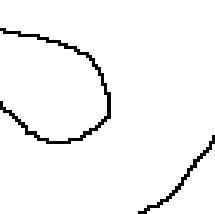
\includegraphics[interpolate=true,width=2.150000in,height=2.140000in]{contents/chapt6/figs/steer/understeer_path-img0.png}}%
\end{pgfscope}%
\begin{pgfscope}%
\pgfpathrectangle{\pgfqpoint{0.520000in}{0.180000in}}{\pgfqpoint{2.140000in}{2.140000in}}%
\pgfusepath{clip}%
\pgfsetbuttcap%
\pgfsetroundjoin%
\pgfsetlinewidth{1.505625pt}%
\definecolor{currentstroke}{rgb}{0.501961,0.501961,0.501961}%
\pgfsetstrokecolor{currentstroke}%
\pgfsetdash{{5.550000pt}{2.400000pt}}{0.000000pt}%
\pgfpathmoveto{\pgfqpoint{0.510000in}{0.703601in}}%
\pgfpathlineto{\pgfqpoint{0.512238in}{0.701484in}}%
\pgfpathlineto{\pgfqpoint{0.558588in}{0.659789in}}%
\pgfpathlineto{\pgfqpoint{0.605896in}{0.620354in}}%
\pgfpathlineto{\pgfqpoint{0.654471in}{0.583901in}}%
\pgfpathlineto{\pgfqpoint{0.704616in}{0.551150in}}%
\pgfpathlineto{\pgfqpoint{0.756638in}{0.522819in}}%
\pgfpathlineto{\pgfqpoint{0.810842in}{0.499630in}}%
\pgfpathlineto{\pgfqpoint{0.867367in}{0.482036in}}%
\pgfpathlineto{\pgfqpoint{0.925915in}{0.469797in}}%
\pgfpathlineto{\pgfqpoint{0.986117in}{0.462557in}}%
\pgfpathlineto{\pgfqpoint{1.047606in}{0.459963in}}%
\pgfpathlineto{\pgfqpoint{1.110012in}{0.461662in}}%
\pgfpathlineto{\pgfqpoint{1.172967in}{0.467300in}}%
\pgfpathlineto{\pgfqpoint{1.236103in}{0.476522in}}%
\pgfpathlineto{\pgfqpoint{1.299050in}{0.488975in}}%
\pgfpathlineto{\pgfqpoint{1.361441in}{0.504305in}}%
\pgfpathlineto{\pgfqpoint{1.422908in}{0.522158in}}%
\pgfpathlineto{\pgfqpoint{1.483152in}{0.542311in}}%
\pgfpathlineto{\pgfqpoint{1.542017in}{0.564791in}}%
\pgfpathlineto{\pgfqpoint{1.599361in}{0.589657in}}%
\pgfpathlineto{\pgfqpoint{1.655043in}{0.616966in}}%
\pgfpathlineto{\pgfqpoint{1.708921in}{0.646777in}}%
\pgfpathlineto{\pgfqpoint{1.760855in}{0.679148in}}%
\pgfpathlineto{\pgfqpoint{1.810704in}{0.714137in}}%
\pgfpathlineto{\pgfqpoint{1.858326in}{0.751803in}}%
\pgfpathlineto{\pgfqpoint{1.903580in}{0.792204in}}%
\pgfpathlineto{\pgfqpoint{1.946326in}{0.835394in}}%
\pgfpathlineto{\pgfqpoint{1.986459in}{0.881308in}}%
\pgfpathlineto{\pgfqpoint{2.023910in}{0.929749in}}%
\pgfpathlineto{\pgfqpoint{2.058615in}{0.980513in}}%
\pgfpathlineto{\pgfqpoint{2.090507in}{1.033395in}}%
\pgfpathlineto{\pgfqpoint{2.119522in}{1.088190in}}%
\pgfpathlineto{\pgfqpoint{2.145594in}{1.144693in}}%
\pgfpathlineto{\pgfqpoint{2.168658in}{1.202701in}}%
\pgfpathlineto{\pgfqpoint{2.188648in}{1.262008in}}%
\pgfpathlineto{\pgfqpoint{2.205498in}{1.322409in}}%
\pgfpathlineto{\pgfqpoint{2.219143in}{1.383700in}}%
\pgfpathlineto{\pgfqpoint{2.229478in}{1.445647in}}%
\pgfpathlineto{\pgfqpoint{2.236361in}{1.507991in}}%
\pgfpathlineto{\pgfqpoint{2.239651in}{1.570469in}}%
\pgfpathlineto{\pgfqpoint{2.239202in}{1.632820in}}%
\pgfpathlineto{\pgfqpoint{2.234873in}{1.694782in}}%
\pgfpathlineto{\pgfqpoint{2.226518in}{1.756093in}}%
\pgfpathlineto{\pgfqpoint{2.213996in}{1.816493in}}%
\pgfpathlineto{\pgfqpoint{2.197163in}{1.875718in}}%
\pgfpathlineto{\pgfqpoint{2.175874in}{1.933508in}}%
\pgfpathlineto{\pgfqpoint{2.150014in}{1.989602in}}%
\pgfpathlineto{\pgfqpoint{2.119740in}{2.043753in}}%
\pgfpathlineto{\pgfqpoint{2.085373in}{2.095721in}}%
\pgfpathlineto{\pgfqpoint{2.047237in}{2.145269in}}%
\pgfpathlineto{\pgfqpoint{2.005657in}{2.192156in}}%
\pgfpathlineto{\pgfqpoint{1.960956in}{2.236143in}}%
\pgfpathlineto{\pgfqpoint{1.913459in}{2.276993in}}%
\pgfpathlineto{\pgfqpoint{1.863489in}{2.314464in}}%
\pgfpathlineto{\pgfqpoint{1.839573in}{2.330000in}}%
\pgfpathlineto{\pgfqpoint{1.839573in}{2.330000in}}%
\pgfusepath{stroke}%
\end{pgfscope}%
\begin{pgfscope}%
\pgfpathrectangle{\pgfqpoint{0.520000in}{0.180000in}}{\pgfqpoint{2.140000in}{2.140000in}}%
\pgfusepath{clip}%
\pgfsetbuttcap%
\pgfsetroundjoin%
\pgfsetlinewidth{1.505625pt}%
\definecolor{currentstroke}{rgb}{1.000000,0.000000,0.000000}%
\pgfsetstrokecolor{currentstroke}%
\pgfsetstrokeopacity{0.500000}%
\pgfsetdash{{9.600000pt}{2.400000pt}{1.500000pt}{2.400000pt}}{0.000000pt}%
\pgfpathmoveto{\pgfqpoint{1.732537in}{0.781910in}}%
\pgfpathlineto{\pgfqpoint{1.755423in}{0.838590in}}%
\pgfpathlineto{\pgfqpoint{1.772636in}{0.897244in}}%
\pgfpathlineto{\pgfqpoint{1.784041in}{0.957298in}}%
\pgfpathlineto{\pgfqpoint{1.789520in}{1.018178in}}%
\pgfpathlineto{\pgfqpoint{1.789021in}{1.079302in}}%
\pgfpathlineto{\pgfqpoint{1.782548in}{1.140085in}}%
\pgfpathlineto{\pgfqpoint{1.770164in}{1.199944in}}%
\pgfpathlineto{\pgfqpoint{1.751986in}{1.258305in}}%
\pgfpathlineto{\pgfqpoint{1.728189in}{1.314608in}}%
\pgfpathlineto{\pgfqpoint{1.699001in}{1.368316in}}%
\pgfpathlineto{\pgfqpoint{1.664701in}{1.418912in}}%
\pgfpathlineto{\pgfqpoint{1.625619in}{1.465913in}}%
\pgfpathlineto{\pgfqpoint{1.582129in}{1.508867in}}%
\pgfpathlineto{\pgfqpoint{1.534648in}{1.547363in}}%
\pgfpathlineto{\pgfqpoint{1.483630in}{1.581032in}}%
\pgfpathlineto{\pgfqpoint{1.429565in}{1.609552in}}%
\pgfpathlineto{\pgfqpoint{1.372970in}{1.632649in}}%
\pgfpathlineto{\pgfqpoint{1.314388in}{1.650102in}}%
\pgfpathlineto{\pgfqpoint{1.254381in}{1.661743in}}%
\pgfpathlineto{\pgfqpoint{1.193523in}{1.667462in}}%
\pgfpathlineto{\pgfqpoint{1.132397in}{1.667203in}}%
\pgfpathlineto{\pgfqpoint{1.071589in}{1.660969in}}%
\pgfpathlineto{\pgfqpoint{1.011683in}{1.648819in}}%
\pgfpathlineto{\pgfqpoint{0.953251in}{1.630870in}}%
\pgfpathlineto{\pgfqpoint{0.896853in}{1.607295in}}%
\pgfpathlineto{\pgfqpoint{0.843015in}{1.578342in}}%
\pgfpathlineto{\pgfqpoint{0.792039in}{1.544588in}}%
\pgfpathlineto{\pgfqpoint{0.741271in}{1.510513in}}%
\pgfpathlineto{\pgfqpoint{0.690359in}{1.476659in}}%
\pgfpathlineto{\pgfqpoint{0.639520in}{1.442692in}}%
\pgfpathlineto{\pgfqpoint{0.588736in}{1.408641in}}%
\pgfpathlineto{\pgfqpoint{0.537940in}{1.374607in}}%
\pgfpathlineto{\pgfqpoint{0.510000in}{1.355910in}}%
\pgfusepath{stroke}%
\end{pgfscope}%
\begin{pgfscope}%
\pgfpathrectangle{\pgfqpoint{0.520000in}{0.180000in}}{\pgfqpoint{2.140000in}{2.140000in}}%
\pgfusepath{clip}%
\pgfsetrectcap%
\pgfsetroundjoin%
\pgfsetlinewidth{1.505625pt}%
\definecolor{currentstroke}{rgb}{1.000000,0.000000,0.000000}%
\pgfsetstrokecolor{currentstroke}%
\pgfsetstrokeopacity{0.500000}%
\pgfsetdash{}{0pt}%
\pgfpathmoveto{\pgfqpoint{1.732537in}{0.781910in}}%
\pgfusepath{stroke}%
\end{pgfscope}%
\begin{pgfscope}%
\pgfpathrectangle{\pgfqpoint{0.520000in}{0.180000in}}{\pgfqpoint{2.140000in}{2.140000in}}%
\pgfusepath{clip}%
\pgfsetbuttcap%
\pgfsetmiterjoin%
\definecolor{currentfill}{rgb}{1.000000,0.000000,0.000000}%
\pgfsetfillcolor{currentfill}%
\pgfsetfillopacity{0.500000}%
\pgfsetlinewidth{1.003750pt}%
\definecolor{currentstroke}{rgb}{1.000000,0.000000,0.000000}%
\pgfsetstrokecolor{currentstroke}%
\pgfsetstrokeopacity{0.500000}%
\pgfsetdash{}{0pt}%
\pgfsys@defobject{currentmarker}{\pgfqpoint{-0.041667in}{-0.041667in}}{\pgfqpoint{0.041667in}{0.041667in}}{%
\pgfpathmoveto{\pgfqpoint{-0.041667in}{-0.041667in}}%
\pgfpathlineto{\pgfqpoint{0.041667in}{-0.041667in}}%
\pgfpathlineto{\pgfqpoint{0.041667in}{0.041667in}}%
\pgfpathlineto{\pgfqpoint{-0.041667in}{0.041667in}}%
\pgfpathlineto{\pgfqpoint{-0.041667in}{-0.041667in}}%
\pgfpathclose%
\pgfusepath{stroke,fill}%
}%
\begin{pgfscope}%
\pgfsys@transformshift{1.732537in}{0.781910in}%
\pgfsys@useobject{currentmarker}{}%
\end{pgfscope}%
\end{pgfscope}%
\begin{pgfscope}%
\pgfpathrectangle{\pgfqpoint{0.520000in}{0.180000in}}{\pgfqpoint{2.140000in}{2.140000in}}%
\pgfusepath{clip}%
\pgfsetrectcap%
\pgfsetroundjoin%
\pgfsetlinewidth{1.505625pt}%
\definecolor{currentstroke}{rgb}{0.121569,0.466667,0.705882}%
\pgfsetstrokecolor{currentstroke}%
\pgfsetdash{}{0pt}%
\pgfpathmoveto{\pgfqpoint{0.510000in}{0.627751in}}%
\pgfpathlineto{\pgfqpoint{0.660868in}{0.585572in}}%
\pgfpathlineto{\pgfqpoint{0.779433in}{0.554375in}}%
\pgfpathlineto{\pgfqpoint{0.869020in}{0.533673in}}%
\pgfpathlineto{\pgfqpoint{0.929206in}{0.522043in}}%
\pgfpathlineto{\pgfqpoint{0.989812in}{0.512863in}}%
\pgfpathlineto{\pgfqpoint{1.050784in}{0.506558in}}%
\pgfpathlineto{\pgfqpoint{1.112005in}{0.503549in}}%
\pgfpathlineto{\pgfqpoint{1.173294in}{0.504266in}}%
\pgfpathlineto{\pgfqpoint{1.234395in}{0.509095in}}%
\pgfpathlineto{\pgfqpoint{1.295000in}{0.518250in}}%
\pgfpathlineto{\pgfqpoint{1.325005in}{0.524508in}}%
\pgfpathlineto{\pgfqpoint{1.354756in}{0.531879in}}%
\pgfpathlineto{\pgfqpoint{1.384218in}{0.540333in}}%
\pgfpathlineto{\pgfqpoint{1.413328in}{0.549928in}}%
\pgfpathlineto{\pgfqpoint{1.442021in}{0.560708in}}%
\pgfpathlineto{\pgfqpoint{1.470266in}{0.572612in}}%
\pgfpathlineto{\pgfqpoint{1.497993in}{0.585676in}}%
\pgfpathlineto{\pgfqpoint{1.525177in}{0.599836in}}%
\pgfpathlineto{\pgfqpoint{1.551745in}{0.615120in}}%
\pgfpathlineto{\pgfqpoint{1.577677in}{0.631461in}}%
\pgfpathlineto{\pgfqpoint{1.602897in}{0.648879in}}%
\pgfpathlineto{\pgfqpoint{1.627392in}{0.667304in}}%
\pgfpathlineto{\pgfqpoint{1.651085in}{0.686749in}}%
\pgfpathlineto{\pgfqpoint{1.673967in}{0.707143in}}%
\pgfpathlineto{\pgfqpoint{1.695962in}{0.728490in}}%
\pgfpathlineto{\pgfqpoint{1.717067in}{0.750717in}}%
\pgfpathlineto{\pgfqpoint{1.737206in}{0.773823in}}%
\pgfpathlineto{\pgfqpoint{1.756382in}{0.797734in}}%
\pgfpathlineto{\pgfqpoint{1.774519in}{0.822443in}}%
\pgfpathlineto{\pgfqpoint{1.791628in}{0.847874in}}%
\pgfpathlineto{\pgfqpoint{1.807718in}{0.873962in}}%
\pgfpathlineto{\pgfqpoint{1.822715in}{0.900694in}}%
\pgfpathlineto{\pgfqpoint{1.836552in}{0.928043in}}%
\pgfpathlineto{\pgfqpoint{1.849256in}{0.955938in}}%
\pgfpathlineto{\pgfqpoint{1.860759in}{0.984348in}}%
\pgfpathlineto{\pgfqpoint{1.871092in}{1.013204in}}%
\pgfpathlineto{\pgfqpoint{1.880188in}{1.042475in}}%
\pgfpathlineto{\pgfqpoint{1.888082in}{1.072091in}}%
\pgfpathlineto{\pgfqpoint{1.894708in}{1.102017in}}%
\pgfpathlineto{\pgfqpoint{1.900108in}{1.132189in}}%
\pgfpathlineto{\pgfqpoint{1.904217in}{1.162563in}}%
\pgfpathlineto{\pgfqpoint{1.907082in}{1.193080in}}%
\pgfpathlineto{\pgfqpoint{1.908643in}{1.223691in}}%
\pgfpathlineto{\pgfqpoint{1.908950in}{1.254340in}}%
\pgfpathlineto{\pgfqpoint{1.907949in}{1.284974in}}%
\pgfpathlineto{\pgfqpoint{1.905693in}{1.315542in}}%
\pgfpathlineto{\pgfqpoint{1.902132in}{1.345985in}}%
\pgfpathlineto{\pgfqpoint{1.897326in}{1.376257in}}%
\pgfpathlineto{\pgfqpoint{1.891326in}{1.406315in}}%
\pgfpathlineto{\pgfqpoint{1.884088in}{1.436099in}}%
\pgfpathlineto{\pgfqpoint{1.875674in}{1.465572in}}%
\pgfpathlineto{\pgfqpoint{1.866051in}{1.494673in}}%
\pgfpathlineto{\pgfqpoint{1.855287in}{1.523372in}}%
\pgfpathlineto{\pgfqpoint{1.843355in}{1.551605in}}%
\pgfpathlineto{\pgfqpoint{1.830327in}{1.579349in}}%
\pgfpathlineto{\pgfqpoint{1.816181in}{1.606540in}}%
\pgfpathlineto{\pgfqpoint{1.800989in}{1.633161in}}%
\pgfpathlineto{\pgfqpoint{1.784736in}{1.659148in}}%
\pgfpathlineto{\pgfqpoint{1.767494in}{1.684489in}}%
\pgfpathlineto{\pgfqpoint{1.749251in}{1.709120in}}%
\pgfpathlineto{\pgfqpoint{1.730079in}{1.733035in}}%
\pgfpathlineto{\pgfqpoint{1.709971in}{1.756167in}}%
\pgfpathlineto{\pgfqpoint{1.688999in}{1.778520in}}%
\pgfpathlineto{\pgfqpoint{1.667157in}{1.800024in}}%
\pgfpathlineto{\pgfqpoint{1.644519in}{1.820687in}}%
\pgfpathlineto{\pgfqpoint{1.621083in}{1.840441in}}%
\pgfpathlineto{\pgfqpoint{1.596920in}{1.859299in}}%
\pgfpathlineto{\pgfqpoint{1.572034in}{1.877193in}}%
\pgfpathlineto{\pgfqpoint{1.520361in}{1.910156in}}%
\pgfpathlineto{\pgfqpoint{1.466536in}{1.939476in}}%
\pgfpathlineto{\pgfqpoint{1.410973in}{1.965357in}}%
\pgfpathlineto{\pgfqpoint{1.354052in}{1.988100in}}%
\pgfpathlineto{\pgfqpoint{1.296116in}{2.008124in}}%
\pgfpathlineto{\pgfqpoint{1.237468in}{2.025959in}}%
\pgfpathlineto{\pgfqpoint{1.148718in}{2.050004in}}%
\pgfpathlineto{\pgfqpoint{0.940536in}{2.101910in}}%
\pgfpathlineto{\pgfqpoint{0.792084in}{2.139967in}}%
\pgfpathlineto{\pgfqpoint{0.673899in}{2.172578in}}%
\pgfpathlineto{\pgfqpoint{0.556299in}{2.207239in}}%
\pgfpathlineto{\pgfqpoint{0.510000in}{2.221437in}}%
\pgfpathlineto{\pgfqpoint{0.510000in}{2.221437in}}%
\pgfusepath{stroke}%
\end{pgfscope}%
\begin{pgfscope}%
\pgfsetrectcap%
\pgfsetmiterjoin%
\pgfsetlinewidth{0.803000pt}%
\definecolor{currentstroke}{rgb}{0.501961,0.501961,0.501961}%
\pgfsetstrokecolor{currentstroke}%
\pgfsetdash{}{0pt}%
\pgfpathmoveto{\pgfqpoint{0.520000in}{0.180000in}}%
\pgfpathlineto{\pgfqpoint{0.520000in}{2.320000in}}%
\pgfusepath{stroke}%
\end{pgfscope}%
\begin{pgfscope}%
\pgfsetrectcap%
\pgfsetmiterjoin%
\pgfsetlinewidth{0.803000pt}%
\definecolor{currentstroke}{rgb}{0.501961,0.501961,0.501961}%
\pgfsetstrokecolor{currentstroke}%
\pgfsetdash{}{0pt}%
\pgfpathmoveto{\pgfqpoint{2.660000in}{0.180000in}}%
\pgfpathlineto{\pgfqpoint{2.660000in}{2.320000in}}%
\pgfusepath{stroke}%
\end{pgfscope}%
\begin{pgfscope}%
\pgfsetrectcap%
\pgfsetmiterjoin%
\pgfsetlinewidth{0.803000pt}%
\definecolor{currentstroke}{rgb}{0.501961,0.501961,0.501961}%
\pgfsetstrokecolor{currentstroke}%
\pgfsetdash{}{0pt}%
\pgfpathmoveto{\pgfqpoint{0.520000in}{0.180000in}}%
\pgfpathlineto{\pgfqpoint{2.660000in}{0.180000in}}%
\pgfusepath{stroke}%
\end{pgfscope}%
\begin{pgfscope}%
\pgfsetrectcap%
\pgfsetmiterjoin%
\pgfsetlinewidth{0.803000pt}%
\definecolor{currentstroke}{rgb}{0.501961,0.501961,0.501961}%
\pgfsetstrokecolor{currentstroke}%
\pgfsetdash{}{0pt}%
\pgfpathmoveto{\pgfqpoint{0.520000in}{2.320000in}}%
\pgfpathlineto{\pgfqpoint{2.660000in}{2.320000in}}%
\pgfusepath{stroke}%
\end{pgfscope}%
\begin{pgfscope}%
\pgfsetbuttcap%
\pgfsetmiterjoin%
\definecolor{currentfill}{rgb}{1.000000,1.000000,1.000000}%
\pgfsetfillcolor{currentfill}%
\pgfsetfillopacity{0.800000}%
\pgfsetlinewidth{1.003750pt}%
\definecolor{currentstroke}{rgb}{0.800000,0.800000,0.800000}%
\pgfsetstrokecolor{currentstroke}%
\pgfsetstrokeopacity{0.800000}%
\pgfsetdash{}{0pt}%
\pgfpathmoveto{\pgfqpoint{2.853000in}{0.623517in}}%
\pgfpathlineto{\pgfqpoint{4.883333in}{0.623517in}}%
\pgfpathquadraticcurveto{\pgfqpoint{4.916667in}{0.623517in}}{\pgfqpoint{4.916667in}{0.656850in}}%
\pgfpathlineto{\pgfqpoint{4.916667in}{1.843150in}}%
\pgfpathquadraticcurveto{\pgfqpoint{4.916667in}{1.876483in}}{\pgfqpoint{4.883333in}{1.876483in}}%
\pgfpathlineto{\pgfqpoint{2.853000in}{1.876483in}}%
\pgfpathquadraticcurveto{\pgfqpoint{2.819667in}{1.876483in}}{\pgfqpoint{2.819667in}{1.843150in}}%
\pgfpathlineto{\pgfqpoint{2.819667in}{0.656850in}}%
\pgfpathquadraticcurveto{\pgfqpoint{2.819667in}{0.623517in}}{\pgfqpoint{2.853000in}{0.623517in}}%
\pgfpathlineto{\pgfqpoint{2.853000in}{0.623517in}}%
\pgfpathclose%
\pgfusepath{stroke,fill}%
\end{pgfscope}%
\begin{pgfscope}%
\pgfsetbuttcap%
\pgfsetroundjoin%
\pgfsetlinewidth{1.505625pt}%
\definecolor{currentstroke}{rgb}{0.501961,0.501961,0.501961}%
\pgfsetstrokecolor{currentstroke}%
\pgfsetdash{{5.550000pt}{2.400000pt}}{0.000000pt}%
\pgfpathmoveto{\pgfqpoint{2.886333in}{1.751483in}}%
\pgfpathlineto{\pgfqpoint{3.053000in}{1.751483in}}%
\pgfpathlineto{\pgfqpoint{3.219667in}{1.751483in}}%
\pgfusepath{stroke}%
\end{pgfscope}%
\begin{pgfscope}%
\definecolor{textcolor}{rgb}{0.000000,0.000000,0.000000}%
\pgfsetstrokecolor{textcolor}%
\pgfsetfillcolor{textcolor}%
\pgftext[x=3.353000in,y=1.693150in,left,base]{\color{textcolor}\rmfamily\fontsize{12.000000}{14.400000}\selectfont Track centerline}%
\end{pgfscope}%
\begin{pgfscope}%
\pgfsetbuttcap%
\pgfsetroundjoin%
\pgfsetlinewidth{1.505625pt}%
\definecolor{currentstroke}{rgb}{1.000000,0.000000,0.000000}%
\pgfsetstrokecolor{currentstroke}%
\pgfsetstrokeopacity{0.500000}%
\pgfsetdash{{9.600000pt}{2.400000pt}{1.500000pt}{2.400000pt}}{0.000000pt}%
\pgfpathmoveto{\pgfqpoint{2.886333in}{1.485816in}}%
\pgfpathlineto{\pgfqpoint{3.053000in}{1.485816in}}%
\pgfpathlineto{\pgfqpoint{3.219667in}{1.485816in}}%
\pgfusepath{stroke}%
\end{pgfscope}%
\begin{pgfscope}%
\definecolor{textcolor}{rgb}{0.000000,0.000000,0.000000}%
\pgfsetstrokecolor{textcolor}%
\pgfsetfillcolor{textcolor}%
\pgftext[x=3.353000in,y=1.427483in,left,base]{\color{textcolor}\rmfamily\fontsize{12.000000}{14.400000}\selectfont Planned path}%
\end{pgfscope}%
\begin{pgfscope}%
\pgfsetrectcap%
\pgfsetroundjoin%
\pgfsetlinewidth{1.505625pt}%
\definecolor{currentstroke}{rgb}{1.000000,0.000000,0.000000}%
\pgfsetstrokecolor{currentstroke}%
\pgfsetstrokeopacity{0.500000}%
\pgfsetdash{}{0pt}%
\pgfpathmoveto{\pgfqpoint{2.886333in}{1.118500in}}%
\pgfpathlineto{\pgfqpoint{3.053000in}{1.118500in}}%
\pgfpathlineto{\pgfqpoint{3.219667in}{1.118500in}}%
\pgfusepath{stroke}%
\end{pgfscope}%
\begin{pgfscope}%
\pgfsetbuttcap%
\pgfsetmiterjoin%
\definecolor{currentfill}{rgb}{1.000000,0.000000,0.000000}%
\pgfsetfillcolor{currentfill}%
\pgfsetfillopacity{0.500000}%
\pgfsetlinewidth{1.003750pt}%
\definecolor{currentstroke}{rgb}{1.000000,0.000000,0.000000}%
\pgfsetstrokecolor{currentstroke}%
\pgfsetstrokeopacity{0.500000}%
\pgfsetdash{}{0pt}%
\pgfsys@defobject{currentmarker}{\pgfqpoint{-0.041667in}{-0.041667in}}{\pgfqpoint{0.041667in}{0.041667in}}{%
\pgfpathmoveto{\pgfqpoint{-0.041667in}{-0.041667in}}%
\pgfpathlineto{\pgfqpoint{0.041667in}{-0.041667in}}%
\pgfpathlineto{\pgfqpoint{0.041667in}{0.041667in}}%
\pgfpathlineto{\pgfqpoint{-0.041667in}{0.041667in}}%
\pgfpathlineto{\pgfqpoint{-0.041667in}{-0.041667in}}%
\pgfpathclose%
\pgfusepath{stroke,fill}%
}%
\begin{pgfscope}%
\pgfsys@transformshift{3.053000in}{1.118500in}%
\pgfsys@useobject{currentmarker}{}%
\end{pgfscope}%
\end{pgfscope}%
\begin{pgfscope}%
\definecolor{textcolor}{rgb}{0.000000,0.000000,0.000000}%
\pgfsetstrokecolor{textcolor}%
\pgfsetfillcolor{textcolor}%
\pgftext[x=3.353000in, y=1.162817in, left, base]{\color{textcolor}\rmfamily\fontsize{12.000000}{14.400000}\selectfont Coordinate at }%
\end{pgfscope}%
\begin{pgfscope}%
\definecolor{textcolor}{rgb}{0.000000,0.000000,0.000000}%
\pgfsetstrokecolor{textcolor}%
\pgfsetfillcolor{textcolor}%
\pgftext[x=3.353000in, y=0.991683in, left, base]{\color{textcolor}\rmfamily\fontsize{12.000000}{14.400000}\selectfont action sampling time}%
\end{pgfscope}%
\begin{pgfscope}%
\pgfsetrectcap%
\pgfsetroundjoin%
\pgfsetlinewidth{1.505625pt}%
\definecolor{currentstroke}{rgb}{0.121569,0.466667,0.705882}%
\pgfsetstrokecolor{currentstroke}%
\pgfsetdash{}{0pt}%
\pgfpathmoveto{\pgfqpoint{2.886333in}{0.782517in}}%
\pgfpathlineto{\pgfqpoint{3.053000in}{0.782517in}}%
\pgfpathlineto{\pgfqpoint{3.219667in}{0.782517in}}%
\pgfusepath{stroke}%
\end{pgfscope}%
\begin{pgfscope}%
\definecolor{textcolor}{rgb}{0.000000,0.000000,0.000000}%
\pgfsetstrokecolor{textcolor}%
\pgfsetfillcolor{textcolor}%
\pgftext[x=3.353000in,y=0.724183in,left,base]{\color{textcolor}\rmfamily\fontsize{12.000000}{14.400000}\selectfont Vehicle path history}%
\end{pgfscope}%
\end{pgfpicture}%
\makeatother%
\endgroup%

    \caption[A snippet of the path taken by a partial end-to-end agent]{A snippet of the path taken by the partial end-to-end agent with steering control utilising the circular arc path construction method.}
    \label{fig:understeer_path}
\end{figure}

Figure \ref{fig:path_method_comparison} also shows the path taken by an agent utilising the Frenet frame polynomial method.
This agent completes the lap in $5.87$ seconds, making it faster than the end-to-end agent, although slightly slower than an agent utilising the circular path.
Furthermore, none of the paths selected by this agent intersect the boundary.
Thus, the constraint placed on the Frenet frame polynomial path can prevent the vehicle from crashing, so long as it follows the path.

This translates into a marked difference between the learning curves of agents using the Frenet frame polynomial path method, and those who do not. 
These learning curves are presented in Figure \ref{fig:path_learning_curves}.
Both the end-to-end agent and partial end-to-end agent utilising the circular path exhibit similar learning curves.
They initially have a $100\%$ failure rate, which then decreases along with lap time. 
However, the failure rate never reaches $0\%$ during training.
In fact, the partial end-to-end agent using the circular path and the end-to-end agent crash $879$ and $559$ times on average during training respectively.

However, our partial end-to-end agent that utilises the Frenet frame displays a learning curve with an entirely different trend.
It successfully complete laps from the start of training.
After only a few crashes, the failure rate decreases to $0\%$ for the remainder of the training period.
In fact, the average number of crashes during training was reduced to a mere $26$.
This comes alongside a significant improvement in training time, as the agent reaches a steady policy after less than $1000$ episodes.
Furthermore, training only took $18.27$ minutes to complete, approximately two thirds of the time that the agent utilising the circular arc path took to train.

\begin{figure}[htb!]
    \centering
    %% Creator: Matplotlib, PGF backend
%%
%% To include the figure in your LaTeX document, write
%%   \input{<filename>.pgf}
%%
%% Make sure the required packages are loaded in your preamble
%%   \usepackage{pgf}
%%
%% Also ensure that all the required font packages are loaded; for instance,
%% the lmodern package is sometimes necessary when using math font.
%%   \usepackage{lmodern}
%%
%% Figures using additional raster images can only be included by \input if
%% they are in the same directory as the main LaTeX file. For loading figures
%% from other directories you can use the `import` package
%%   \usepackage{import}
%%
%% and then include the figures with
%%   \import{<path to file>}{<filename>.pgf}
%%
%% Matplotlib used the following preamble
%%   \usepackage{fontspec}
%%
\begingroup%
\makeatletter%
\begin{pgfpicture}%
\pgfpathrectangle{\pgfpointorigin}{\pgfqpoint{5.500000in}{2.800000in}}%
\pgfusepath{use as bounding box, clip}%
\begin{pgfscope}%
\pgfsetbuttcap%
\pgfsetmiterjoin%
\definecolor{currentfill}{rgb}{1.000000,1.000000,1.000000}%
\pgfsetfillcolor{currentfill}%
\pgfsetlinewidth{0.000000pt}%
\definecolor{currentstroke}{rgb}{1.000000,1.000000,1.000000}%
\pgfsetstrokecolor{currentstroke}%
\pgfsetdash{}{0pt}%
\pgfpathmoveto{\pgfqpoint{0.000000in}{0.000000in}}%
\pgfpathlineto{\pgfqpoint{5.500000in}{0.000000in}}%
\pgfpathlineto{\pgfqpoint{5.500000in}{2.800000in}}%
\pgfpathlineto{\pgfqpoint{0.000000in}{2.800000in}}%
\pgfpathlineto{\pgfqpoint{0.000000in}{0.000000in}}%
\pgfpathclose%
\pgfusepath{fill}%
\end{pgfscope}%
\begin{pgfscope}%
\pgfsetbuttcap%
\pgfsetmiterjoin%
\definecolor{currentfill}{rgb}{1.000000,1.000000,1.000000}%
\pgfsetfillcolor{currentfill}%
\pgfsetlinewidth{0.000000pt}%
\definecolor{currentstroke}{rgb}{0.000000,0.000000,0.000000}%
\pgfsetstrokecolor{currentstroke}%
\pgfsetstrokeopacity{0.000000}%
\pgfsetdash{}{0pt}%
\pgfpathmoveto{\pgfqpoint{0.695622in}{0.924000in}}%
\pgfpathlineto{\pgfqpoint{2.700763in}{0.924000in}}%
\pgfpathlineto{\pgfqpoint{2.700763in}{2.620000in}}%
\pgfpathlineto{\pgfqpoint{0.695622in}{2.620000in}}%
\pgfpathlineto{\pgfqpoint{0.695622in}{0.924000in}}%
\pgfpathclose%
\pgfusepath{fill}%
\end{pgfscope}%
\begin{pgfscope}%
\pgfpathrectangle{\pgfqpoint{0.695622in}{0.924000in}}{\pgfqpoint{2.005141in}{1.696000in}}%
\pgfusepath{clip}%
\pgfsetbuttcap%
\pgfsetroundjoin%
\definecolor{currentfill}{rgb}{0.121569,0.466667,0.705882}%
\pgfsetfillcolor{currentfill}%
\pgfsetfillopacity{0.150000}%
\pgfsetlinewidth{0.000000pt}%
\definecolor{currentstroke}{rgb}{0.000000,0.000000,0.000000}%
\pgfsetstrokecolor{currentstroke}%
\pgfsetdash{}{0pt}%
\pgfpathmoveto{\pgfqpoint{0.695622in}{2.542909in}}%
\pgfpathlineto{\pgfqpoint{0.695622in}{2.542909in}}%
\pgfpathlineto{\pgfqpoint{0.762460in}{2.542909in}}%
\pgfpathlineto{\pgfqpoint{0.829298in}{2.632925in}}%
\pgfpathlineto{\pgfqpoint{0.896136in}{2.493676in}}%
\pgfpathlineto{\pgfqpoint{0.962974in}{2.401632in}}%
\pgfpathlineto{\pgfqpoint{1.029812in}{2.317787in}}%
\pgfpathlineto{\pgfqpoint{1.096650in}{1.948676in}}%
\pgfpathlineto{\pgfqpoint{1.163488in}{1.789645in}}%
\pgfpathlineto{\pgfqpoint{1.230326in}{1.694582in}}%
\pgfpathlineto{\pgfqpoint{1.297164in}{1.583989in}}%
\pgfpathlineto{\pgfqpoint{1.364003in}{1.504963in}}%
\pgfpathlineto{\pgfqpoint{1.430841in}{1.488749in}}%
\pgfpathlineto{\pgfqpoint{1.497679in}{1.464315in}}%
\pgfpathlineto{\pgfqpoint{1.564517in}{1.454330in}}%
\pgfpathlineto{\pgfqpoint{1.631355in}{1.470139in}}%
\pgfpathlineto{\pgfqpoint{1.698193in}{1.460411in}}%
\pgfpathlineto{\pgfqpoint{1.765031in}{1.443174in}}%
\pgfpathlineto{\pgfqpoint{1.831869in}{1.462720in}}%
\pgfpathlineto{\pgfqpoint{1.898707in}{1.469327in}}%
\pgfpathlineto{\pgfqpoint{1.965545in}{1.450505in}}%
\pgfpathlineto{\pgfqpoint{2.032383in}{1.453211in}}%
\pgfpathlineto{\pgfqpoint{2.099221in}{1.460905in}}%
\pgfpathlineto{\pgfqpoint{2.166059in}{1.434713in}}%
\pgfpathlineto{\pgfqpoint{2.232897in}{1.428044in}}%
\pgfpathlineto{\pgfqpoint{2.299735in}{1.433319in}}%
\pgfpathlineto{\pgfqpoint{2.366573in}{1.439396in}}%
\pgfpathlineto{\pgfqpoint{2.433411in}{1.459906in}}%
\pgfpathlineto{\pgfqpoint{2.500249in}{1.471443in}}%
\pgfpathlineto{\pgfqpoint{2.567087in}{1.467808in}}%
\pgfpathlineto{\pgfqpoint{2.633925in}{1.452647in}}%
\pgfpathlineto{\pgfqpoint{2.633925in}{0.900367in}}%
\pgfpathlineto{\pgfqpoint{2.633925in}{0.900367in}}%
\pgfpathlineto{\pgfqpoint{2.567087in}{0.891362in}}%
\pgfpathlineto{\pgfqpoint{2.500249in}{0.887727in}}%
\pgfpathlineto{\pgfqpoint{2.433411in}{0.886954in}}%
\pgfpathlineto{\pgfqpoint{2.366573in}{0.884895in}}%
\pgfpathlineto{\pgfqpoint{2.299735in}{0.884817in}}%
\pgfpathlineto{\pgfqpoint{2.232897in}{0.888041in}}%
\pgfpathlineto{\pgfqpoint{2.166059in}{0.885475in}}%
\pgfpathlineto{\pgfqpoint{2.099221in}{0.881851in}}%
\pgfpathlineto{\pgfqpoint{2.032383in}{0.883390in}}%
\pgfpathlineto{\pgfqpoint{1.965545in}{0.881993in}}%
\pgfpathlineto{\pgfqpoint{1.898707in}{0.883688in}}%
\pgfpathlineto{\pgfqpoint{1.831869in}{0.880036in}}%
\pgfpathlineto{\pgfqpoint{1.765031in}{0.881118in}}%
\pgfpathlineto{\pgfqpoint{1.698193in}{0.884397in}}%
\pgfpathlineto{\pgfqpoint{1.631355in}{0.886979in}}%
\pgfpathlineto{\pgfqpoint{1.564517in}{0.892529in}}%
\pgfpathlineto{\pgfqpoint{1.497679in}{0.901010in}}%
\pgfpathlineto{\pgfqpoint{1.430841in}{0.901195in}}%
\pgfpathlineto{\pgfqpoint{1.364003in}{0.897292in}}%
\pgfpathlineto{\pgfqpoint{1.297164in}{0.910590in}}%
\pgfpathlineto{\pgfqpoint{1.230326in}{0.929251in}}%
\pgfpathlineto{\pgfqpoint{1.163488in}{0.983959in}}%
\pgfpathlineto{\pgfqpoint{1.096650in}{1.083437in}}%
\pgfpathlineto{\pgfqpoint{1.029812in}{1.243652in}}%
\pgfpathlineto{\pgfqpoint{0.962974in}{1.343586in}}%
\pgfpathlineto{\pgfqpoint{0.896136in}{1.492551in}}%
\pgfpathlineto{\pgfqpoint{0.829298in}{1.747185in}}%
\pgfpathlineto{\pgfqpoint{0.762460in}{2.542909in}}%
\pgfpathlineto{\pgfqpoint{0.695622in}{2.542909in}}%
\pgfpathlineto{\pgfqpoint{0.695622in}{2.542909in}}%
\pgfpathclose%
\pgfusepath{fill}%
\end{pgfscope}%
\begin{pgfscope}%
\pgfpathrectangle{\pgfqpoint{0.695622in}{0.924000in}}{\pgfqpoint{2.005141in}{1.696000in}}%
\pgfusepath{clip}%
\pgfsetbuttcap%
\pgfsetroundjoin%
\definecolor{currentfill}{rgb}{1.000000,0.498039,0.054902}%
\pgfsetfillcolor{currentfill}%
\pgfsetfillopacity{0.150000}%
\pgfsetlinewidth{0.000000pt}%
\definecolor{currentstroke}{rgb}{0.000000,0.000000,0.000000}%
\pgfsetstrokecolor{currentstroke}%
\pgfsetdash{}{0pt}%
\pgfpathmoveto{\pgfqpoint{0.695622in}{2.542909in}}%
\pgfpathlineto{\pgfqpoint{0.695622in}{2.542909in}}%
\pgfpathlineto{\pgfqpoint{0.762460in}{2.542909in}}%
\pgfpathlineto{\pgfqpoint{0.829298in}{2.655483in}}%
\pgfpathlineto{\pgfqpoint{0.896136in}{2.557628in}}%
\pgfpathlineto{\pgfqpoint{0.962974in}{2.509116in}}%
\pgfpathlineto{\pgfqpoint{1.029812in}{2.484952in}}%
\pgfpathlineto{\pgfqpoint{1.096650in}{2.282126in}}%
\pgfpathlineto{\pgfqpoint{1.163488in}{2.248876in}}%
\pgfpathlineto{\pgfqpoint{1.230326in}{2.189339in}}%
\pgfpathlineto{\pgfqpoint{1.297164in}{2.087957in}}%
\pgfpathlineto{\pgfqpoint{1.364003in}{1.933035in}}%
\pgfpathlineto{\pgfqpoint{1.430841in}{1.851689in}}%
\pgfpathlineto{\pgfqpoint{1.497679in}{1.763300in}}%
\pgfpathlineto{\pgfqpoint{1.564517in}{1.727420in}}%
\pgfpathlineto{\pgfqpoint{1.631355in}{1.695391in}}%
\pgfpathlineto{\pgfqpoint{1.698193in}{1.678509in}}%
\pgfpathlineto{\pgfqpoint{1.765031in}{1.655025in}}%
\pgfpathlineto{\pgfqpoint{1.831869in}{1.637459in}}%
\pgfpathlineto{\pgfqpoint{1.898707in}{1.579782in}}%
\pgfpathlineto{\pgfqpoint{1.965545in}{1.582848in}}%
\pgfpathlineto{\pgfqpoint{2.032383in}{1.561905in}}%
\pgfpathlineto{\pgfqpoint{2.099221in}{1.536791in}}%
\pgfpathlineto{\pgfqpoint{2.166059in}{1.528992in}}%
\pgfpathlineto{\pgfqpoint{2.232897in}{1.568004in}}%
\pgfpathlineto{\pgfqpoint{2.299735in}{1.540503in}}%
\pgfpathlineto{\pgfqpoint{2.366573in}{1.559361in}}%
\pgfpathlineto{\pgfqpoint{2.433411in}{1.547798in}}%
\pgfpathlineto{\pgfqpoint{2.500249in}{1.544428in}}%
\pgfpathlineto{\pgfqpoint{2.567087in}{1.507392in}}%
\pgfpathlineto{\pgfqpoint{2.633925in}{1.480460in}}%
\pgfpathlineto{\pgfqpoint{2.700763in}{1.476099in}}%
\pgfpathlineto{\pgfqpoint{2.767601in}{1.464126in}}%
\pgfpathlineto{\pgfqpoint{2.834439in}{1.468579in}}%
\pgfpathlineto{\pgfqpoint{2.901277in}{1.463575in}}%
\pgfpathlineto{\pgfqpoint{2.968115in}{1.445162in}}%
\pgfpathlineto{\pgfqpoint{3.034953in}{1.410082in}}%
\pgfpathlineto{\pgfqpoint{3.101791in}{1.405710in}}%
\pgfpathlineto{\pgfqpoint{3.101791in}{0.889859in}}%
\pgfpathlineto{\pgfqpoint{3.101791in}{0.889859in}}%
\pgfpathlineto{\pgfqpoint{3.034953in}{0.891642in}}%
\pgfpathlineto{\pgfqpoint{2.968115in}{0.893492in}}%
\pgfpathlineto{\pgfqpoint{2.901277in}{0.897646in}}%
\pgfpathlineto{\pgfqpoint{2.834439in}{0.894694in}}%
\pgfpathlineto{\pgfqpoint{2.767601in}{0.895044in}}%
\pgfpathlineto{\pgfqpoint{2.700763in}{0.893328in}}%
\pgfpathlineto{\pgfqpoint{2.633925in}{0.893071in}}%
\pgfpathlineto{\pgfqpoint{2.567087in}{0.898966in}}%
\pgfpathlineto{\pgfqpoint{2.500249in}{0.909117in}}%
\pgfpathlineto{\pgfqpoint{2.433411in}{0.918057in}}%
\pgfpathlineto{\pgfqpoint{2.366573in}{0.918805in}}%
\pgfpathlineto{\pgfqpoint{2.299735in}{0.908940in}}%
\pgfpathlineto{\pgfqpoint{2.232897in}{0.908110in}}%
\pgfpathlineto{\pgfqpoint{2.166059in}{0.899934in}}%
\pgfpathlineto{\pgfqpoint{2.099221in}{0.894187in}}%
\pgfpathlineto{\pgfqpoint{2.032383in}{0.899847in}}%
\pgfpathlineto{\pgfqpoint{1.965545in}{0.903524in}}%
\pgfpathlineto{\pgfqpoint{1.898707in}{0.912745in}}%
\pgfpathlineto{\pgfqpoint{1.831869in}{0.928928in}}%
\pgfpathlineto{\pgfqpoint{1.765031in}{0.950343in}}%
\pgfpathlineto{\pgfqpoint{1.698193in}{0.957634in}}%
\pgfpathlineto{\pgfqpoint{1.631355in}{0.971527in}}%
\pgfpathlineto{\pgfqpoint{1.564517in}{0.974376in}}%
\pgfpathlineto{\pgfqpoint{1.497679in}{0.995943in}}%
\pgfpathlineto{\pgfqpoint{1.430841in}{1.030653in}}%
\pgfpathlineto{\pgfqpoint{1.364003in}{1.082664in}}%
\pgfpathlineto{\pgfqpoint{1.297164in}{1.178044in}}%
\pgfpathlineto{\pgfqpoint{1.230326in}{1.285931in}}%
\pgfpathlineto{\pgfqpoint{1.163488in}{1.361802in}}%
\pgfpathlineto{\pgfqpoint{1.096650in}{1.412670in}}%
\pgfpathlineto{\pgfqpoint{1.029812in}{1.544264in}}%
\pgfpathlineto{\pgfqpoint{0.962974in}{1.548823in}}%
\pgfpathlineto{\pgfqpoint{0.896136in}{1.568609in}}%
\pgfpathlineto{\pgfqpoint{0.829298in}{1.714400in}}%
\pgfpathlineto{\pgfqpoint{0.762460in}{2.542909in}}%
\pgfpathlineto{\pgfqpoint{0.695622in}{2.542909in}}%
\pgfpathlineto{\pgfqpoint{0.695622in}{2.542909in}}%
\pgfpathclose%
\pgfusepath{fill}%
\end{pgfscope}%
\begin{pgfscope}%
\pgfpathrectangle{\pgfqpoint{0.695622in}{0.924000in}}{\pgfqpoint{2.005141in}{1.696000in}}%
\pgfusepath{clip}%
\pgfsetbuttcap%
\pgfsetroundjoin%
\definecolor{currentfill}{rgb}{0.172549,0.627451,0.172549}%
\pgfsetfillcolor{currentfill}%
\pgfsetfillopacity{0.150000}%
\pgfsetlinewidth{0.000000pt}%
\definecolor{currentstroke}{rgb}{0.000000,0.000000,0.000000}%
\pgfsetstrokecolor{currentstroke}%
\pgfsetdash{}{0pt}%
\pgfpathmoveto{\pgfqpoint{0.695622in}{1.001091in}}%
\pgfpathlineto{\pgfqpoint{0.695622in}{1.001091in}}%
\pgfpathlineto{\pgfqpoint{0.762460in}{1.249918in}}%
\pgfpathlineto{\pgfqpoint{0.829298in}{1.229108in}}%
\pgfpathlineto{\pgfqpoint{0.896136in}{1.218008in}}%
\pgfpathlineto{\pgfqpoint{0.962974in}{1.191007in}}%
\pgfpathlineto{\pgfqpoint{1.029812in}{1.170745in}}%
\pgfpathlineto{\pgfqpoint{1.096650in}{1.132245in}}%
\pgfpathlineto{\pgfqpoint{1.163488in}{1.100156in}}%
\pgfpathlineto{\pgfqpoint{1.230326in}{1.063151in}}%
\pgfpathlineto{\pgfqpoint{1.297164in}{1.057306in}}%
\pgfpathlineto{\pgfqpoint{1.364003in}{1.068595in}}%
\pgfpathlineto{\pgfqpoint{1.430841in}{1.078585in}}%
\pgfpathlineto{\pgfqpoint{1.497679in}{1.083230in}}%
\pgfpathlineto{\pgfqpoint{1.564517in}{1.078585in}}%
\pgfpathlineto{\pgfqpoint{1.631355in}{1.078585in}}%
\pgfpathlineto{\pgfqpoint{1.698193in}{1.087688in}}%
\pgfpathlineto{\pgfqpoint{1.765031in}{1.087688in}}%
\pgfpathlineto{\pgfqpoint{1.831869in}{1.078585in}}%
\pgfpathlineto{\pgfqpoint{1.898707in}{1.083230in}}%
\pgfpathlineto{\pgfqpoint{1.965545in}{1.083230in}}%
\pgfpathlineto{\pgfqpoint{2.032383in}{1.068595in}}%
\pgfpathlineto{\pgfqpoint{2.099221in}{1.043819in}}%
\pgfpathlineto{\pgfqpoint{2.166059in}{1.050933in}}%
\pgfpathlineto{\pgfqpoint{2.232897in}{1.057306in}}%
\pgfpathlineto{\pgfqpoint{2.299735in}{1.050933in}}%
\pgfpathlineto{\pgfqpoint{2.366573in}{1.050933in}}%
\pgfpathlineto{\pgfqpoint{2.433411in}{1.063151in}}%
\pgfpathlineto{\pgfqpoint{2.500249in}{1.057306in}}%
\pgfpathlineto{\pgfqpoint{2.567087in}{1.050933in}}%
\pgfpathlineto{\pgfqpoint{2.633925in}{1.057306in}}%
\pgfpathlineto{\pgfqpoint{2.700763in}{1.063151in}}%
\pgfpathlineto{\pgfqpoint{2.767601in}{1.057306in}}%
\pgfpathlineto{\pgfqpoint{2.834439in}{1.063151in}}%
\pgfpathlineto{\pgfqpoint{2.901277in}{1.068595in}}%
\pgfpathlineto{\pgfqpoint{2.901277in}{0.947948in}}%
\pgfpathlineto{\pgfqpoint{2.901277in}{0.947948in}}%
\pgfpathlineto{\pgfqpoint{2.834439in}{0.951341in}}%
\pgfpathlineto{\pgfqpoint{2.767601in}{0.955134in}}%
\pgfpathlineto{\pgfqpoint{2.700763in}{0.951341in}}%
\pgfpathlineto{\pgfqpoint{2.633925in}{0.955134in}}%
\pgfpathlineto{\pgfqpoint{2.567087in}{0.959456in}}%
\pgfpathlineto{\pgfqpoint{2.500249in}{0.955134in}}%
\pgfpathlineto{\pgfqpoint{2.433411in}{0.951341in}}%
\pgfpathlineto{\pgfqpoint{2.366573in}{0.959456in}}%
\pgfpathlineto{\pgfqpoint{2.299735in}{0.959456in}}%
\pgfpathlineto{\pgfqpoint{2.232897in}{0.955134in}}%
\pgfpathlineto{\pgfqpoint{2.166059in}{0.959456in}}%
\pgfpathlineto{\pgfqpoint{2.099221in}{0.964518in}}%
\pgfpathlineto{\pgfqpoint{2.032383in}{0.947948in}}%
\pgfpathlineto{\pgfqpoint{1.965545in}{0.939468in}}%
\pgfpathlineto{\pgfqpoint{1.898707in}{0.939468in}}%
\pgfpathlineto{\pgfqpoint{1.831869in}{0.942062in}}%
\pgfpathlineto{\pgfqpoint{1.765031in}{0.937062in}}%
\pgfpathlineto{\pgfqpoint{1.698193in}{0.937062in}}%
\pgfpathlineto{\pgfqpoint{1.631355in}{0.942062in}}%
\pgfpathlineto{\pgfqpoint{1.564517in}{0.942062in}}%
\pgfpathlineto{\pgfqpoint{1.497679in}{0.939468in}}%
\pgfpathlineto{\pgfqpoint{1.430841in}{0.942062in}}%
\pgfpathlineto{\pgfqpoint{1.364003in}{0.947948in}}%
\pgfpathlineto{\pgfqpoint{1.297164in}{0.955134in}}%
\pgfpathlineto{\pgfqpoint{1.230326in}{0.951341in}}%
\pgfpathlineto{\pgfqpoint{1.163488in}{0.930749in}}%
\pgfpathlineto{\pgfqpoint{1.096650in}{0.917125in}}%
\pgfpathlineto{\pgfqpoint{1.029812in}{0.905296in}}%
\pgfpathlineto{\pgfqpoint{0.962974in}{0.900890in}}%
\pgfpathlineto{\pgfqpoint{0.896136in}{0.896864in}}%
\pgfpathlineto{\pgfqpoint{0.829298in}{0.895806in}}%
\pgfpathlineto{\pgfqpoint{0.762460in}{0.894742in}}%
\pgfpathlineto{\pgfqpoint{0.695622in}{1.001091in}}%
\pgfpathlineto{\pgfqpoint{0.695622in}{1.001091in}}%
\pgfpathclose%
\pgfusepath{fill}%
\end{pgfscope}%
\begin{pgfscope}%
\pgfpathrectangle{\pgfqpoint{0.695622in}{0.924000in}}{\pgfqpoint{2.005141in}{1.696000in}}%
\pgfusepath{clip}%
\pgfsetrectcap%
\pgfsetroundjoin%
\pgfsetlinewidth{0.803000pt}%
\definecolor{currentstroke}{rgb}{0.690196,0.690196,0.690196}%
\pgfsetstrokecolor{currentstroke}%
\pgfsetdash{}{0pt}%
\pgfpathmoveto{\pgfqpoint{0.695622in}{0.924000in}}%
\pgfpathlineto{\pgfqpoint{0.695622in}{2.620000in}}%
\pgfusepath{stroke}%
\end{pgfscope}%
\begin{pgfscope}%
\definecolor{textcolor}{rgb}{0.000000,0.000000,0.000000}%
\pgfsetstrokecolor{textcolor}%
\pgfsetfillcolor{textcolor}%
\pgftext[x=0.695622in,y=0.875389in,,top]{\color{textcolor}\rmfamily\fontsize{12.000000}{14.400000}\selectfont 0}%
\end{pgfscope}%
\begin{pgfscope}%
\pgfpathrectangle{\pgfqpoint{0.695622in}{0.924000in}}{\pgfqpoint{2.005141in}{1.696000in}}%
\pgfusepath{clip}%
\pgfsetrectcap%
\pgfsetroundjoin%
\pgfsetlinewidth{0.803000pt}%
\definecolor{currentstroke}{rgb}{0.690196,0.690196,0.690196}%
\pgfsetstrokecolor{currentstroke}%
\pgfsetdash{}{0pt}%
\pgfpathmoveto{\pgfqpoint{1.364003in}{0.924000in}}%
\pgfpathlineto{\pgfqpoint{1.364003in}{2.620000in}}%
\pgfusepath{stroke}%
\end{pgfscope}%
\begin{pgfscope}%
\definecolor{textcolor}{rgb}{0.000000,0.000000,0.000000}%
\pgfsetstrokecolor{textcolor}%
\pgfsetfillcolor{textcolor}%
\pgftext[x=1.364003in,y=0.875389in,,top]{\color{textcolor}\rmfamily\fontsize{12.000000}{14.400000}\selectfont 1}%
\end{pgfscope}%
\begin{pgfscope}%
\pgfpathrectangle{\pgfqpoint{0.695622in}{0.924000in}}{\pgfqpoint{2.005141in}{1.696000in}}%
\pgfusepath{clip}%
\pgfsetrectcap%
\pgfsetroundjoin%
\pgfsetlinewidth{0.803000pt}%
\definecolor{currentstroke}{rgb}{0.690196,0.690196,0.690196}%
\pgfsetstrokecolor{currentstroke}%
\pgfsetdash{}{0pt}%
\pgfpathmoveto{\pgfqpoint{2.032383in}{0.924000in}}%
\pgfpathlineto{\pgfqpoint{2.032383in}{2.620000in}}%
\pgfusepath{stroke}%
\end{pgfscope}%
\begin{pgfscope}%
\definecolor{textcolor}{rgb}{0.000000,0.000000,0.000000}%
\pgfsetstrokecolor{textcolor}%
\pgfsetfillcolor{textcolor}%
\pgftext[x=2.032383in,y=0.875389in,,top]{\color{textcolor}\rmfamily\fontsize{12.000000}{14.400000}\selectfont 2}%
\end{pgfscope}%
\begin{pgfscope}%
\pgfpathrectangle{\pgfqpoint{0.695622in}{0.924000in}}{\pgfqpoint{2.005141in}{1.696000in}}%
\pgfusepath{clip}%
\pgfsetrectcap%
\pgfsetroundjoin%
\pgfsetlinewidth{0.803000pt}%
\definecolor{currentstroke}{rgb}{0.690196,0.690196,0.690196}%
\pgfsetstrokecolor{currentstroke}%
\pgfsetdash{}{0pt}%
\pgfpathmoveto{\pgfqpoint{2.700763in}{0.924000in}}%
\pgfpathlineto{\pgfqpoint{2.700763in}{2.620000in}}%
\pgfusepath{stroke}%
\end{pgfscope}%
\begin{pgfscope}%
\definecolor{textcolor}{rgb}{0.000000,0.000000,0.000000}%
\pgfsetstrokecolor{textcolor}%
\pgfsetfillcolor{textcolor}%
\pgftext[x=2.700763in,y=0.875389in,,top]{\color{textcolor}\rmfamily\fontsize{12.000000}{14.400000}\selectfont 3}%
\end{pgfscope}%
\begin{pgfscope}%
\definecolor{textcolor}{rgb}{0.000000,0.000000,0.000000}%
\pgfsetstrokecolor{textcolor}%
\pgfsetfillcolor{textcolor}%
\pgftext[x=1.698193in,y=0.671833in,,top]{\color{textcolor}\rmfamily\fontsize{12.000000}{14.400000}\selectfont Episodes \(\displaystyle \times 10^3\)}%
\end{pgfscope}%
\begin{pgfscope}%
\pgfpathrectangle{\pgfqpoint{0.695622in}{0.924000in}}{\pgfqpoint{2.005141in}{1.696000in}}%
\pgfusepath{clip}%
\pgfsetrectcap%
\pgfsetroundjoin%
\pgfsetlinewidth{0.803000pt}%
\definecolor{currentstroke}{rgb}{0.690196,0.690196,0.690196}%
\pgfsetstrokecolor{currentstroke}%
\pgfsetdash{}{0pt}%
\pgfpathmoveto{\pgfqpoint{0.695622in}{1.001091in}}%
\pgfpathlineto{\pgfqpoint{2.700763in}{1.001091in}}%
\pgfusepath{stroke}%
\end{pgfscope}%
\begin{pgfscope}%
\definecolor{textcolor}{rgb}{0.000000,0.000000,0.000000}%
\pgfsetstrokecolor{textcolor}%
\pgfsetfillcolor{textcolor}%
\pgftext[x=0.565415in, y=0.943258in, left, base]{\color{textcolor}\rmfamily\fontsize{12.000000}{14.400000}\selectfont \(\displaystyle {0}\)}%
\end{pgfscope}%
\begin{pgfscope}%
\pgfpathrectangle{\pgfqpoint{0.695622in}{0.924000in}}{\pgfqpoint{2.005141in}{1.696000in}}%
\pgfusepath{clip}%
\pgfsetrectcap%
\pgfsetroundjoin%
\pgfsetlinewidth{0.803000pt}%
\definecolor{currentstroke}{rgb}{0.690196,0.690196,0.690196}%
\pgfsetstrokecolor{currentstroke}%
\pgfsetdash{}{0pt}%
\pgfpathmoveto{\pgfqpoint{0.695622in}{1.386545in}}%
\pgfpathlineto{\pgfqpoint{2.700763in}{1.386545in}}%
\pgfusepath{stroke}%
\end{pgfscope}%
\begin{pgfscope}%
\definecolor{textcolor}{rgb}{0.000000,0.000000,0.000000}%
\pgfsetstrokecolor{textcolor}%
\pgfsetfillcolor{textcolor}%
\pgftext[x=0.483818in, y=1.328712in, left, base]{\color{textcolor}\rmfamily\fontsize{12.000000}{14.400000}\selectfont \(\displaystyle {25}\)}%
\end{pgfscope}%
\begin{pgfscope}%
\pgfpathrectangle{\pgfqpoint{0.695622in}{0.924000in}}{\pgfqpoint{2.005141in}{1.696000in}}%
\pgfusepath{clip}%
\pgfsetrectcap%
\pgfsetroundjoin%
\pgfsetlinewidth{0.803000pt}%
\definecolor{currentstroke}{rgb}{0.690196,0.690196,0.690196}%
\pgfsetstrokecolor{currentstroke}%
\pgfsetdash{}{0pt}%
\pgfpathmoveto{\pgfqpoint{0.695622in}{1.772000in}}%
\pgfpathlineto{\pgfqpoint{2.700763in}{1.772000in}}%
\pgfusepath{stroke}%
\end{pgfscope}%
\begin{pgfscope}%
\definecolor{textcolor}{rgb}{0.000000,0.000000,0.000000}%
\pgfsetstrokecolor{textcolor}%
\pgfsetfillcolor{textcolor}%
\pgftext[x=0.483818in, y=1.714167in, left, base]{\color{textcolor}\rmfamily\fontsize{12.000000}{14.400000}\selectfont \(\displaystyle {50}\)}%
\end{pgfscope}%
\begin{pgfscope}%
\pgfpathrectangle{\pgfqpoint{0.695622in}{0.924000in}}{\pgfqpoint{2.005141in}{1.696000in}}%
\pgfusepath{clip}%
\pgfsetrectcap%
\pgfsetroundjoin%
\pgfsetlinewidth{0.803000pt}%
\definecolor{currentstroke}{rgb}{0.690196,0.690196,0.690196}%
\pgfsetstrokecolor{currentstroke}%
\pgfsetdash{}{0pt}%
\pgfpathmoveto{\pgfqpoint{0.695622in}{2.157455in}}%
\pgfpathlineto{\pgfqpoint{2.700763in}{2.157455in}}%
\pgfusepath{stroke}%
\end{pgfscope}%
\begin{pgfscope}%
\definecolor{textcolor}{rgb}{0.000000,0.000000,0.000000}%
\pgfsetstrokecolor{textcolor}%
\pgfsetfillcolor{textcolor}%
\pgftext[x=0.483818in, y=2.099621in, left, base]{\color{textcolor}\rmfamily\fontsize{12.000000}{14.400000}\selectfont \(\displaystyle {75}\)}%
\end{pgfscope}%
\begin{pgfscope}%
\pgfpathrectangle{\pgfqpoint{0.695622in}{0.924000in}}{\pgfqpoint{2.005141in}{1.696000in}}%
\pgfusepath{clip}%
\pgfsetrectcap%
\pgfsetroundjoin%
\pgfsetlinewidth{0.803000pt}%
\definecolor{currentstroke}{rgb}{0.690196,0.690196,0.690196}%
\pgfsetstrokecolor{currentstroke}%
\pgfsetdash{}{0pt}%
\pgfpathmoveto{\pgfqpoint{0.695622in}{2.542909in}}%
\pgfpathlineto{\pgfqpoint{2.700763in}{2.542909in}}%
\pgfusepath{stroke}%
\end{pgfscope}%
\begin{pgfscope}%
\definecolor{textcolor}{rgb}{0.000000,0.000000,0.000000}%
\pgfsetstrokecolor{textcolor}%
\pgfsetfillcolor{textcolor}%
\pgftext[x=0.402222in, y=2.485076in, left, base]{\color{textcolor}\rmfamily\fontsize{12.000000}{14.400000}\selectfont \(\displaystyle {100}\)}%
\end{pgfscope}%
\begin{pgfscope}%
\definecolor{textcolor}{rgb}{0.000000,0.000000,0.000000}%
\pgfsetstrokecolor{textcolor}%
\pgfsetfillcolor{textcolor}%
\pgftext[x=0.346666in,y=1.772000in,,bottom,rotate=90.000000]{\color{textcolor}\rmfamily\fontsize{12.000000}{14.400000}\selectfont Failure rate [\%]}%
\end{pgfscope}%
\begin{pgfscope}%
\pgfpathrectangle{\pgfqpoint{0.695622in}{0.924000in}}{\pgfqpoint{2.005141in}{1.696000in}}%
\pgfusepath{clip}%
\pgfsetrectcap%
\pgfsetroundjoin%
\pgfsetlinewidth{1.505625pt}%
\definecolor{currentstroke}{rgb}{0.121569,0.466667,0.705882}%
\pgfsetstrokecolor{currentstroke}%
\pgfsetdash{}{0pt}%
\pgfpathmoveto{\pgfqpoint{0.695622in}{2.542909in}}%
\pgfpathlineto{\pgfqpoint{0.762460in}{2.542909in}}%
\pgfpathlineto{\pgfqpoint{0.829298in}{2.190055in}}%
\pgfpathlineto{\pgfqpoint{0.896136in}{1.993113in}}%
\pgfpathlineto{\pgfqpoint{0.962974in}{1.872609in}}%
\pgfpathlineto{\pgfqpoint{1.029812in}{1.780720in}}%
\pgfpathlineto{\pgfqpoint{1.096650in}{1.516056in}}%
\pgfpathlineto{\pgfqpoint{1.163488in}{1.386802in}}%
\pgfpathlineto{\pgfqpoint{1.230326in}{1.311917in}}%
\pgfpathlineto{\pgfqpoint{1.297164in}{1.247289in}}%
\pgfpathlineto{\pgfqpoint{1.364003in}{1.201127in}}%
\pgfpathlineto{\pgfqpoint{1.430841in}{1.194972in}}%
\pgfpathlineto{\pgfqpoint{1.497679in}{1.182662in}}%
\pgfpathlineto{\pgfqpoint{1.564517in}{1.173430in}}%
\pgfpathlineto{\pgfqpoint{1.631355in}{1.178559in}}%
\pgfpathlineto{\pgfqpoint{1.698193in}{1.172404in}}%
\pgfpathlineto{\pgfqpoint{1.765031in}{1.162146in}}%
\pgfpathlineto{\pgfqpoint{1.831869in}{1.171378in}}%
\pgfpathlineto{\pgfqpoint{1.898707in}{1.176507in}}%
\pgfpathlineto{\pgfqpoint{1.965545in}{1.166249in}}%
\pgfpathlineto{\pgfqpoint{2.032383in}{1.168301in}}%
\pgfpathlineto{\pgfqpoint{2.099221in}{1.171378in}}%
\pgfpathlineto{\pgfqpoint{2.166059in}{1.160094in}}%
\pgfpathlineto{\pgfqpoint{2.232897in}{1.158042in}}%
\pgfpathlineto{\pgfqpoint{2.299735in}{1.159068in}}%
\pgfpathlineto{\pgfqpoint{2.366573in}{1.162146in}}%
\pgfpathlineto{\pgfqpoint{2.433411in}{1.173430in}}%
\pgfpathlineto{\pgfqpoint{2.500249in}{1.179585in}}%
\pgfpathlineto{\pgfqpoint{2.567087in}{1.179585in}}%
\pgfpathlineto{\pgfqpoint{2.633925in}{1.176507in}}%
\pgfusepath{stroke}%
\end{pgfscope}%
\begin{pgfscope}%
\pgfpathrectangle{\pgfqpoint{0.695622in}{0.924000in}}{\pgfqpoint{2.005141in}{1.696000in}}%
\pgfusepath{clip}%
\pgfsetrectcap%
\pgfsetroundjoin%
\pgfsetlinewidth{1.505625pt}%
\definecolor{currentstroke}{rgb}{1.000000,0.498039,0.054902}%
\pgfsetstrokecolor{currentstroke}%
\pgfsetdash{}{0pt}%
\pgfpathmoveto{\pgfqpoint{0.695622in}{2.542909in}}%
\pgfpathlineto{\pgfqpoint{0.762460in}{2.542909in}}%
\pgfpathlineto{\pgfqpoint{0.829298in}{2.184941in}}%
\pgfpathlineto{\pgfqpoint{0.896136in}{2.063118in}}%
\pgfpathlineto{\pgfqpoint{0.962974in}{2.028970in}}%
\pgfpathlineto{\pgfqpoint{1.029812in}{2.014608in}}%
\pgfpathlineto{\pgfqpoint{1.096650in}{1.847398in}}%
\pgfpathlineto{\pgfqpoint{1.163488in}{1.805339in}}%
\pgfpathlineto{\pgfqpoint{1.230326in}{1.737635in}}%
\pgfpathlineto{\pgfqpoint{1.297164in}{1.633000in}}%
\pgfpathlineto{\pgfqpoint{1.364003in}{1.507850in}}%
\pgfpathlineto{\pgfqpoint{1.430841in}{1.441171in}}%
\pgfpathlineto{\pgfqpoint{1.497679in}{1.379621in}}%
\pgfpathlineto{\pgfqpoint{1.564517in}{1.350898in}}%
\pgfpathlineto{\pgfqpoint{1.631355in}{1.333459in}}%
\pgfpathlineto{\pgfqpoint{1.698193in}{1.318071in}}%
\pgfpathlineto{\pgfqpoint{1.765031in}{1.302684in}}%
\pgfpathlineto{\pgfqpoint{1.831869in}{1.283193in}}%
\pgfpathlineto{\pgfqpoint{1.898707in}{1.246264in}}%
\pgfpathlineto{\pgfqpoint{1.965545in}{1.243186in}}%
\pgfpathlineto{\pgfqpoint{2.032383in}{1.230876in}}%
\pgfpathlineto{\pgfqpoint{2.099221in}{1.215489in}}%
\pgfpathlineto{\pgfqpoint{2.166059in}{1.214463in}}%
\pgfpathlineto{\pgfqpoint{2.232897in}{1.238057in}}%
\pgfpathlineto{\pgfqpoint{2.299735in}{1.224721in}}%
\pgfpathlineto{\pgfqpoint{2.366573in}{1.239083in}}%
\pgfpathlineto{\pgfqpoint{2.433411in}{1.232928in}}%
\pgfpathlineto{\pgfqpoint{2.500249in}{1.226773in}}%
\pgfpathlineto{\pgfqpoint{2.567087in}{1.203179in}}%
\pgfpathlineto{\pgfqpoint{2.633925in}{1.186766in}}%
\pgfpathlineto{\pgfqpoint{2.700763in}{1.184714in}}%
\pgfpathlineto{\pgfqpoint{2.710763in}{1.183947in}}%
\pgfusepath{stroke}%
\end{pgfscope}%
\begin{pgfscope}%
\pgfpathrectangle{\pgfqpoint{0.695622in}{0.924000in}}{\pgfqpoint{2.005141in}{1.696000in}}%
\pgfusepath{clip}%
\pgfsetrectcap%
\pgfsetroundjoin%
\pgfsetlinewidth{1.505625pt}%
\definecolor{currentstroke}{rgb}{0.172549,0.627451,0.172549}%
\pgfsetstrokecolor{currentstroke}%
\pgfsetdash{}{0pt}%
\pgfpathmoveto{\pgfqpoint{0.695622in}{1.001091in}}%
\pgfpathlineto{\pgfqpoint{0.762460in}{1.072330in}}%
\pgfpathlineto{\pgfqpoint{0.829298in}{1.062457in}}%
\pgfpathlineto{\pgfqpoint{0.896136in}{1.057436in}}%
\pgfpathlineto{\pgfqpoint{0.962974in}{1.045948in}}%
\pgfpathlineto{\pgfqpoint{1.029812in}{1.038021in}}%
\pgfpathlineto{\pgfqpoint{1.096650in}{1.024685in}}%
\pgfpathlineto{\pgfqpoint{1.163488in}{1.015452in}}%
\pgfpathlineto{\pgfqpoint{1.230326in}{1.007246in}}%
\pgfpathlineto{\pgfqpoint{1.297164in}{1.006220in}}%
\pgfpathlineto{\pgfqpoint{1.364003in}{1.008272in}}%
\pgfpathlineto{\pgfqpoint{1.430841in}{1.010323in}}%
\pgfpathlineto{\pgfqpoint{1.497679in}{1.011349in}}%
\pgfpathlineto{\pgfqpoint{1.564517in}{1.010323in}}%
\pgfpathlineto{\pgfqpoint{1.631355in}{1.010323in}}%
\pgfpathlineto{\pgfqpoint{1.698193in}{1.012375in}}%
\pgfpathlineto{\pgfqpoint{1.765031in}{1.012375in}}%
\pgfpathlineto{\pgfqpoint{1.831869in}{1.010323in}}%
\pgfpathlineto{\pgfqpoint{1.898707in}{1.011349in}}%
\pgfpathlineto{\pgfqpoint{1.965545in}{1.011349in}}%
\pgfpathlineto{\pgfqpoint{2.032383in}{1.008272in}}%
\pgfpathlineto{\pgfqpoint{2.099221in}{1.004168in}}%
\pgfpathlineto{\pgfqpoint{2.166059in}{1.005194in}}%
\pgfpathlineto{\pgfqpoint{2.232897in}{1.006220in}}%
\pgfpathlineto{\pgfqpoint{2.299735in}{1.005194in}}%
\pgfpathlineto{\pgfqpoint{2.366573in}{1.005194in}}%
\pgfpathlineto{\pgfqpoint{2.433411in}{1.007246in}}%
\pgfpathlineto{\pgfqpoint{2.500249in}{1.006220in}}%
\pgfpathlineto{\pgfqpoint{2.567087in}{1.005194in}}%
\pgfpathlineto{\pgfqpoint{2.633925in}{1.006220in}}%
\pgfpathlineto{\pgfqpoint{2.700763in}{1.007246in}}%
\pgfpathlineto{\pgfqpoint{2.710763in}{1.007092in}}%
\pgfusepath{stroke}%
\end{pgfscope}%
\begin{pgfscope}%
\pgfpathrectangle{\pgfqpoint{0.695622in}{0.924000in}}{\pgfqpoint{2.005141in}{1.696000in}}%
\pgfusepath{clip}%
\pgfsetbuttcap%
\pgfsetroundjoin%
\pgfsetlinewidth{1.505625pt}%
\definecolor{currentstroke}{rgb}{0.000000,0.000000,0.000000}%
\pgfsetstrokecolor{currentstroke}%
\pgfsetdash{{5.550000pt}{2.400000pt}}{0.000000pt}%
\pgfpathmoveto{\pgfqpoint{0.695622in}{2.542909in}}%
\pgfpathlineto{\pgfqpoint{2.710763in}{2.542909in}}%
\pgfusepath{stroke}%
\end{pgfscope}%
\begin{pgfscope}%
\pgfpathrectangle{\pgfqpoint{0.695622in}{0.924000in}}{\pgfqpoint{2.005141in}{1.696000in}}%
\pgfusepath{clip}%
\pgfsetbuttcap%
\pgfsetroundjoin%
\pgfsetlinewidth{1.505625pt}%
\definecolor{currentstroke}{rgb}{0.000000,0.000000,0.000000}%
\pgfsetstrokecolor{currentstroke}%
\pgfsetdash{{5.550000pt}{2.400000pt}}{0.000000pt}%
\pgfpathmoveto{\pgfqpoint{0.695622in}{1.001091in}}%
\pgfpathlineto{\pgfqpoint{2.710763in}{1.001091in}}%
\pgfusepath{stroke}%
\end{pgfscope}%
\begin{pgfscope}%
\pgfsetrectcap%
\pgfsetmiterjoin%
\pgfsetlinewidth{0.803000pt}%
\definecolor{currentstroke}{rgb}{0.501961,0.501961,0.501961}%
\pgfsetstrokecolor{currentstroke}%
\pgfsetdash{}{0pt}%
\pgfpathmoveto{\pgfqpoint{0.695622in}{0.924000in}}%
\pgfpathlineto{\pgfqpoint{0.695622in}{2.620000in}}%
\pgfusepath{stroke}%
\end{pgfscope}%
\begin{pgfscope}%
\pgfsetrectcap%
\pgfsetmiterjoin%
\pgfsetlinewidth{0.803000pt}%
\definecolor{currentstroke}{rgb}{0.501961,0.501961,0.501961}%
\pgfsetstrokecolor{currentstroke}%
\pgfsetdash{}{0pt}%
\pgfpathmoveto{\pgfqpoint{2.700763in}{0.924000in}}%
\pgfpathlineto{\pgfqpoint{2.700763in}{2.620000in}}%
\pgfusepath{stroke}%
\end{pgfscope}%
\begin{pgfscope}%
\pgfsetrectcap%
\pgfsetmiterjoin%
\pgfsetlinewidth{0.803000pt}%
\definecolor{currentstroke}{rgb}{0.501961,0.501961,0.501961}%
\pgfsetstrokecolor{currentstroke}%
\pgfsetdash{}{0pt}%
\pgfpathmoveto{\pgfqpoint{0.695622in}{0.924000in}}%
\pgfpathlineto{\pgfqpoint{2.700763in}{0.924000in}}%
\pgfusepath{stroke}%
\end{pgfscope}%
\begin{pgfscope}%
\pgfsetrectcap%
\pgfsetmiterjoin%
\pgfsetlinewidth{0.803000pt}%
\definecolor{currentstroke}{rgb}{0.501961,0.501961,0.501961}%
\pgfsetstrokecolor{currentstroke}%
\pgfsetdash{}{0pt}%
\pgfpathmoveto{\pgfqpoint{0.695622in}{2.620000in}}%
\pgfpathlineto{\pgfqpoint{2.700763in}{2.620000in}}%
\pgfusepath{stroke}%
\end{pgfscope}%
\begin{pgfscope}%
\pgfsetbuttcap%
\pgfsetmiterjoin%
\definecolor{currentfill}{rgb}{1.000000,1.000000,1.000000}%
\pgfsetfillcolor{currentfill}%
\pgfsetlinewidth{0.000000pt}%
\definecolor{currentstroke}{rgb}{0.000000,0.000000,0.000000}%
\pgfsetstrokecolor{currentstroke}%
\pgfsetstrokeopacity{0.000000}%
\pgfsetdash{}{0pt}%
\pgfpathmoveto{\pgfqpoint{3.274026in}{0.924000in}}%
\pgfpathlineto{\pgfqpoint{5.279167in}{0.924000in}}%
\pgfpathlineto{\pgfqpoint{5.279167in}{2.620000in}}%
\pgfpathlineto{\pgfqpoint{3.274026in}{2.620000in}}%
\pgfpathlineto{\pgfqpoint{3.274026in}{0.924000in}}%
\pgfpathclose%
\pgfusepath{fill}%
\end{pgfscope}%
\begin{pgfscope}%
\pgfpathrectangle{\pgfqpoint{3.274026in}{0.924000in}}{\pgfqpoint{2.005141in}{1.696000in}}%
\pgfusepath{clip}%
\pgfsetbuttcap%
\pgfsetroundjoin%
\definecolor{currentfill}{rgb}{0.121569,0.466667,0.705882}%
\pgfsetfillcolor{currentfill}%
\pgfsetfillopacity{0.150000}%
\pgfsetlinewidth{0.000000pt}%
\definecolor{currentstroke}{rgb}{0.000000,0.000000,0.000000}%
\pgfsetstrokecolor{currentstroke}%
\pgfsetdash{}{0pt}%
\pgfpathmoveto{\pgfqpoint{3.407702in}{2.152698in}}%
\pgfpathlineto{\pgfqpoint{3.407702in}{2.542909in}}%
\pgfpathlineto{\pgfqpoint{3.474540in}{2.482401in}}%
\pgfpathlineto{\pgfqpoint{3.541378in}{2.449215in}}%
\pgfpathlineto{\pgfqpoint{3.608216in}{2.394249in}}%
\pgfpathlineto{\pgfqpoint{3.675054in}{2.333857in}}%
\pgfpathlineto{\pgfqpoint{3.741892in}{2.185737in}}%
\pgfpathlineto{\pgfqpoint{3.808730in}{2.007290in}}%
\pgfpathlineto{\pgfqpoint{3.875568in}{1.895225in}}%
\pgfpathlineto{\pgfqpoint{3.942406in}{1.779650in}}%
\pgfpathlineto{\pgfqpoint{4.009244in}{1.690267in}}%
\pgfpathlineto{\pgfqpoint{4.076082in}{1.645282in}}%
\pgfpathlineto{\pgfqpoint{4.142920in}{1.617725in}}%
\pgfpathlineto{\pgfqpoint{4.209758in}{1.567561in}}%
\pgfpathlineto{\pgfqpoint{4.276596in}{1.517146in}}%
\pgfpathlineto{\pgfqpoint{4.343434in}{1.466368in}}%
\pgfpathlineto{\pgfqpoint{4.410272in}{1.424318in}}%
\pgfpathlineto{\pgfqpoint{4.477110in}{1.388596in}}%
\pgfpathlineto{\pgfqpoint{4.543948in}{1.380350in}}%
\pgfpathlineto{\pgfqpoint{4.610786in}{1.370640in}}%
\pgfpathlineto{\pgfqpoint{4.677624in}{1.356179in}}%
\pgfpathlineto{\pgfqpoint{4.744462in}{1.346854in}}%
\pgfpathlineto{\pgfqpoint{4.811300in}{1.341621in}}%
\pgfpathlineto{\pgfqpoint{4.878139in}{1.335283in}}%
\pgfpathlineto{\pgfqpoint{4.944977in}{1.328318in}}%
\pgfpathlineto{\pgfqpoint{5.011815in}{1.321204in}}%
\pgfpathlineto{\pgfqpoint{5.078653in}{1.313691in}}%
\pgfpathlineto{\pgfqpoint{5.145491in}{1.310284in}}%
\pgfpathlineto{\pgfqpoint{5.212329in}{1.310182in}}%
\pgfpathlineto{\pgfqpoint{5.212329in}{1.189445in}}%
\pgfpathlineto{\pgfqpoint{5.212329in}{1.189445in}}%
\pgfpathlineto{\pgfqpoint{5.145491in}{1.187067in}}%
\pgfpathlineto{\pgfqpoint{5.078653in}{1.190697in}}%
\pgfpathlineto{\pgfqpoint{5.011815in}{1.192655in}}%
\pgfpathlineto{\pgfqpoint{4.944977in}{1.194471in}}%
\pgfpathlineto{\pgfqpoint{4.878139in}{1.199298in}}%
\pgfpathlineto{\pgfqpoint{4.811300in}{1.205756in}}%
\pgfpathlineto{\pgfqpoint{4.744462in}{1.206982in}}%
\pgfpathlineto{\pgfqpoint{4.677624in}{1.207650in}}%
\pgfpathlineto{\pgfqpoint{4.610786in}{1.216445in}}%
\pgfpathlineto{\pgfqpoint{4.543948in}{1.222474in}}%
\pgfpathlineto{\pgfqpoint{4.477110in}{1.229691in}}%
\pgfpathlineto{\pgfqpoint{4.410272in}{1.239226in}}%
\pgfpathlineto{\pgfqpoint{4.343434in}{1.262007in}}%
\pgfpathlineto{\pgfqpoint{4.276596in}{1.277195in}}%
\pgfpathlineto{\pgfqpoint{4.209758in}{1.310743in}}%
\pgfpathlineto{\pgfqpoint{4.142920in}{1.355394in}}%
\pgfpathlineto{\pgfqpoint{4.076082in}{1.391240in}}%
\pgfpathlineto{\pgfqpoint{4.009244in}{1.412695in}}%
\pgfpathlineto{\pgfqpoint{3.942406in}{1.439441in}}%
\pgfpathlineto{\pgfqpoint{3.875568in}{1.461974in}}%
\pgfpathlineto{\pgfqpoint{3.808730in}{1.502575in}}%
\pgfpathlineto{\pgfqpoint{3.741892in}{1.599590in}}%
\pgfpathlineto{\pgfqpoint{3.675054in}{1.725368in}}%
\pgfpathlineto{\pgfqpoint{3.608216in}{1.792338in}}%
\pgfpathlineto{\pgfqpoint{3.541378in}{1.881158in}}%
\pgfpathlineto{\pgfqpoint{3.474540in}{2.084356in}}%
\pgfpathlineto{\pgfqpoint{3.407702in}{2.152698in}}%
\pgfpathlineto{\pgfqpoint{3.407702in}{2.152698in}}%
\pgfpathclose%
\pgfusepath{fill}%
\end{pgfscope}%
\begin{pgfscope}%
\pgfpathrectangle{\pgfqpoint{3.274026in}{0.924000in}}{\pgfqpoint{2.005141in}{1.696000in}}%
\pgfusepath{clip}%
\pgfsetbuttcap%
\pgfsetroundjoin%
\definecolor{currentfill}{rgb}{1.000000,0.498039,0.054902}%
\pgfsetfillcolor{currentfill}%
\pgfsetfillopacity{0.150000}%
\pgfsetlinewidth{0.000000pt}%
\definecolor{currentstroke}{rgb}{0.000000,0.000000,0.000000}%
\pgfsetstrokecolor{currentstroke}%
\pgfsetdash{}{0pt}%
\pgfpathmoveto{\pgfqpoint{3.407702in}{2.039612in}}%
\pgfpathlineto{\pgfqpoint{3.407702in}{2.525584in}}%
\pgfpathlineto{\pgfqpoint{3.474540in}{2.379104in}}%
\pgfpathlineto{\pgfqpoint{3.541378in}{2.287108in}}%
\pgfpathlineto{\pgfqpoint{3.608216in}{2.210143in}}%
\pgfpathlineto{\pgfqpoint{3.675054in}{2.116602in}}%
\pgfpathlineto{\pgfqpoint{3.741892in}{1.790035in}}%
\pgfpathlineto{\pgfqpoint{3.808730in}{1.543293in}}%
\pgfpathlineto{\pgfqpoint{3.875568in}{1.374431in}}%
\pgfpathlineto{\pgfqpoint{3.942406in}{1.287787in}}%
\pgfpathlineto{\pgfqpoint{4.009244in}{1.238221in}}%
\pgfpathlineto{\pgfqpoint{4.076082in}{1.219365in}}%
\pgfpathlineto{\pgfqpoint{4.142920in}{1.207098in}}%
\pgfpathlineto{\pgfqpoint{4.209758in}{1.196128in}}%
\pgfpathlineto{\pgfqpoint{4.276596in}{1.182032in}}%
\pgfpathlineto{\pgfqpoint{4.343434in}{1.167089in}}%
\pgfpathlineto{\pgfqpoint{4.410272in}{1.156452in}}%
\pgfpathlineto{\pgfqpoint{4.477110in}{1.150640in}}%
\pgfpathlineto{\pgfqpoint{4.543948in}{1.147251in}}%
\pgfpathlineto{\pgfqpoint{4.610786in}{1.144634in}}%
\pgfpathlineto{\pgfqpoint{4.677624in}{1.136293in}}%
\pgfpathlineto{\pgfqpoint{4.744462in}{1.132750in}}%
\pgfpathlineto{\pgfqpoint{4.811300in}{1.125014in}}%
\pgfpathlineto{\pgfqpoint{4.878139in}{1.118570in}}%
\pgfpathlineto{\pgfqpoint{4.944977in}{1.117671in}}%
\pgfpathlineto{\pgfqpoint{5.011815in}{1.120627in}}%
\pgfpathlineto{\pgfqpoint{5.078653in}{1.122918in}}%
\pgfpathlineto{\pgfqpoint{5.145491in}{1.121404in}}%
\pgfpathlineto{\pgfqpoint{5.212329in}{1.119673in}}%
\pgfpathlineto{\pgfqpoint{5.279167in}{1.123048in}}%
\pgfpathlineto{\pgfqpoint{5.346005in}{1.120336in}}%
\pgfpathlineto{\pgfqpoint{5.412843in}{1.113283in}}%
\pgfpathlineto{\pgfqpoint{5.479681in}{1.112177in}}%
\pgfpathlineto{\pgfqpoint{5.546519in}{1.112656in}}%
\pgfpathlineto{\pgfqpoint{5.613357in}{1.104364in}}%
\pgfpathlineto{\pgfqpoint{5.680195in}{1.105778in}}%
\pgfpathlineto{\pgfqpoint{5.680195in}{1.001435in}}%
\pgfpathlineto{\pgfqpoint{5.680195in}{1.001435in}}%
\pgfpathlineto{\pgfqpoint{5.613357in}{1.001091in}}%
\pgfpathlineto{\pgfqpoint{5.546519in}{1.003658in}}%
\pgfpathlineto{\pgfqpoint{5.479681in}{1.003571in}}%
\pgfpathlineto{\pgfqpoint{5.412843in}{1.005048in}}%
\pgfpathlineto{\pgfqpoint{5.346005in}{1.005907in}}%
\pgfpathlineto{\pgfqpoint{5.279167in}{1.008208in}}%
\pgfpathlineto{\pgfqpoint{5.212329in}{1.007328in}}%
\pgfpathlineto{\pgfqpoint{5.145491in}{1.007320in}}%
\pgfpathlineto{\pgfqpoint{5.078653in}{1.006154in}}%
\pgfpathlineto{\pgfqpoint{5.011815in}{1.006828in}}%
\pgfpathlineto{\pgfqpoint{4.944977in}{1.007971in}}%
\pgfpathlineto{\pgfqpoint{4.878139in}{1.011676in}}%
\pgfpathlineto{\pgfqpoint{4.811300in}{1.017146in}}%
\pgfpathlineto{\pgfqpoint{4.744462in}{1.023344in}}%
\pgfpathlineto{\pgfqpoint{4.677624in}{1.027816in}}%
\pgfpathlineto{\pgfqpoint{4.610786in}{1.033633in}}%
\pgfpathlineto{\pgfqpoint{4.543948in}{1.037880in}}%
\pgfpathlineto{\pgfqpoint{4.477110in}{1.041193in}}%
\pgfpathlineto{\pgfqpoint{4.410272in}{1.045275in}}%
\pgfpathlineto{\pgfqpoint{4.343434in}{1.051998in}}%
\pgfpathlineto{\pgfqpoint{4.276596in}{1.058402in}}%
\pgfpathlineto{\pgfqpoint{4.209758in}{1.067230in}}%
\pgfpathlineto{\pgfqpoint{4.142920in}{1.077913in}}%
\pgfpathlineto{\pgfqpoint{4.076082in}{1.088123in}}%
\pgfpathlineto{\pgfqpoint{4.009244in}{1.097279in}}%
\pgfpathlineto{\pgfqpoint{3.942406in}{1.102489in}}%
\pgfpathlineto{\pgfqpoint{3.875568in}{1.105962in}}%
\pgfpathlineto{\pgfqpoint{3.808730in}{1.122523in}}%
\pgfpathlineto{\pgfqpoint{3.741892in}{1.182584in}}%
\pgfpathlineto{\pgfqpoint{3.675054in}{1.305968in}}%
\pgfpathlineto{\pgfqpoint{3.608216in}{1.454187in}}%
\pgfpathlineto{\pgfqpoint{3.541378in}{1.635530in}}%
\pgfpathlineto{\pgfqpoint{3.474540in}{1.846178in}}%
\pgfpathlineto{\pgfqpoint{3.407702in}{2.039612in}}%
\pgfpathlineto{\pgfqpoint{3.407702in}{2.039612in}}%
\pgfpathclose%
\pgfusepath{fill}%
\end{pgfscope}%
\begin{pgfscope}%
\pgfpathrectangle{\pgfqpoint{3.274026in}{0.924000in}}{\pgfqpoint{2.005141in}{1.696000in}}%
\pgfusepath{clip}%
\pgfsetbuttcap%
\pgfsetroundjoin%
\definecolor{currentfill}{rgb}{0.172549,0.627451,0.172549}%
\pgfsetfillcolor{currentfill}%
\pgfsetfillopacity{0.150000}%
\pgfsetlinewidth{0.000000pt}%
\definecolor{currentstroke}{rgb}{0.000000,0.000000,0.000000}%
\pgfsetstrokecolor{currentstroke}%
\pgfsetdash{}{0pt}%
\pgfpathmoveto{\pgfqpoint{3.274026in}{2.121689in}}%
\pgfpathlineto{\pgfqpoint{3.274026in}{2.121689in}}%
\pgfpathlineto{\pgfqpoint{3.340864in}{1.313672in}}%
\pgfpathlineto{\pgfqpoint{3.407702in}{1.243937in}}%
\pgfpathlineto{\pgfqpoint{3.474540in}{1.213883in}}%
\pgfpathlineto{\pgfqpoint{3.541378in}{1.197119in}}%
\pgfpathlineto{\pgfqpoint{3.608216in}{1.187310in}}%
\pgfpathlineto{\pgfqpoint{3.675054in}{1.120825in}}%
\pgfpathlineto{\pgfqpoint{3.741892in}{1.121698in}}%
\pgfpathlineto{\pgfqpoint{3.808730in}{1.122170in}}%
\pgfpathlineto{\pgfqpoint{3.875568in}{1.121401in}}%
\pgfpathlineto{\pgfqpoint{3.942406in}{1.118588in}}%
\pgfpathlineto{\pgfqpoint{4.009244in}{1.118017in}}%
\pgfpathlineto{\pgfqpoint{4.076082in}{1.116164in}}%
\pgfpathlineto{\pgfqpoint{4.142920in}{1.113829in}}%
\pgfpathlineto{\pgfqpoint{4.209758in}{1.112672in}}%
\pgfpathlineto{\pgfqpoint{4.276596in}{1.113883in}}%
\pgfpathlineto{\pgfqpoint{4.343434in}{1.113945in}}%
\pgfpathlineto{\pgfqpoint{4.410272in}{1.113570in}}%
\pgfpathlineto{\pgfqpoint{4.477110in}{1.114314in}}%
\pgfpathlineto{\pgfqpoint{4.543948in}{1.116062in}}%
\pgfpathlineto{\pgfqpoint{4.610786in}{1.114106in}}%
\pgfpathlineto{\pgfqpoint{4.677624in}{1.115132in}}%
\pgfpathlineto{\pgfqpoint{4.744462in}{1.114202in}}%
\pgfpathlineto{\pgfqpoint{4.811300in}{1.113852in}}%
\pgfpathlineto{\pgfqpoint{4.878139in}{1.114999in}}%
\pgfpathlineto{\pgfqpoint{4.944977in}{1.118340in}}%
\pgfpathlineto{\pgfqpoint{5.011815in}{1.118435in}}%
\pgfpathlineto{\pgfqpoint{5.078653in}{1.119075in}}%
\pgfpathlineto{\pgfqpoint{5.145491in}{1.119687in}}%
\pgfpathlineto{\pgfqpoint{5.212329in}{1.117066in}}%
\pgfpathlineto{\pgfqpoint{5.279167in}{1.115147in}}%
\pgfpathlineto{\pgfqpoint{5.346005in}{1.116609in}}%
\pgfpathlineto{\pgfqpoint{5.412843in}{1.117580in}}%
\pgfpathlineto{\pgfqpoint{5.479681in}{1.117295in}}%
\pgfpathlineto{\pgfqpoint{5.479681in}{1.078669in}}%
\pgfpathlineto{\pgfqpoint{5.479681in}{1.078669in}}%
\pgfpathlineto{\pgfqpoint{5.412843in}{1.078292in}}%
\pgfpathlineto{\pgfqpoint{5.346005in}{1.075111in}}%
\pgfpathlineto{\pgfqpoint{5.279167in}{1.072892in}}%
\pgfpathlineto{\pgfqpoint{5.212329in}{1.069405in}}%
\pgfpathlineto{\pgfqpoint{5.145491in}{1.069284in}}%
\pgfpathlineto{\pgfqpoint{5.078653in}{1.068162in}}%
\pgfpathlineto{\pgfqpoint{5.011815in}{1.068743in}}%
\pgfpathlineto{\pgfqpoint{4.944977in}{1.068682in}}%
\pgfpathlineto{\pgfqpoint{4.878139in}{1.069694in}}%
\pgfpathlineto{\pgfqpoint{4.811300in}{1.069418in}}%
\pgfpathlineto{\pgfqpoint{4.744462in}{1.070070in}}%
\pgfpathlineto{\pgfqpoint{4.677624in}{1.070424in}}%
\pgfpathlineto{\pgfqpoint{4.610786in}{1.071534in}}%
\pgfpathlineto{\pgfqpoint{4.543948in}{1.071463in}}%
\pgfpathlineto{\pgfqpoint{4.477110in}{1.071503in}}%
\pgfpathlineto{\pgfqpoint{4.410272in}{1.071174in}}%
\pgfpathlineto{\pgfqpoint{4.343434in}{1.071269in}}%
\pgfpathlineto{\pgfqpoint{4.276596in}{1.070702in}}%
\pgfpathlineto{\pgfqpoint{4.209758in}{1.071551in}}%
\pgfpathlineto{\pgfqpoint{4.142920in}{1.072720in}}%
\pgfpathlineto{\pgfqpoint{4.076082in}{1.073709in}}%
\pgfpathlineto{\pgfqpoint{4.009244in}{1.074494in}}%
\pgfpathlineto{\pgfqpoint{3.942406in}{1.076017in}}%
\pgfpathlineto{\pgfqpoint{3.875568in}{1.075133in}}%
\pgfpathlineto{\pgfqpoint{3.808730in}{1.075488in}}%
\pgfpathlineto{\pgfqpoint{3.741892in}{1.075579in}}%
\pgfpathlineto{\pgfqpoint{3.675054in}{1.076202in}}%
\pgfpathlineto{\pgfqpoint{3.608216in}{1.037547in}}%
\pgfpathlineto{\pgfqpoint{3.541378in}{1.032993in}}%
\pgfpathlineto{\pgfqpoint{3.474540in}{1.026914in}}%
\pgfpathlineto{\pgfqpoint{3.407702in}{1.020475in}}%
\pgfpathlineto{\pgfqpoint{3.340864in}{1.014897in}}%
\pgfpathlineto{\pgfqpoint{3.274026in}{2.121689in}}%
\pgfpathlineto{\pgfqpoint{3.274026in}{2.121689in}}%
\pgfpathclose%
\pgfusepath{fill}%
\end{pgfscope}%
\begin{pgfscope}%
\pgfpathrectangle{\pgfqpoint{3.274026in}{0.924000in}}{\pgfqpoint{2.005141in}{1.696000in}}%
\pgfusepath{clip}%
\pgfsetrectcap%
\pgfsetroundjoin%
\pgfsetlinewidth{0.803000pt}%
\definecolor{currentstroke}{rgb}{0.690196,0.690196,0.690196}%
\pgfsetstrokecolor{currentstroke}%
\pgfsetdash{}{0pt}%
\pgfpathmoveto{\pgfqpoint{3.274026in}{0.924000in}}%
\pgfpathlineto{\pgfqpoint{3.274026in}{2.620000in}}%
\pgfusepath{stroke}%
\end{pgfscope}%
\begin{pgfscope}%
\definecolor{textcolor}{rgb}{0.000000,0.000000,0.000000}%
\pgfsetstrokecolor{textcolor}%
\pgfsetfillcolor{textcolor}%
\pgftext[x=3.274026in,y=0.875389in,,top]{\color{textcolor}\rmfamily\fontsize{12.000000}{14.400000}\selectfont 0}%
\end{pgfscope}%
\begin{pgfscope}%
\pgfpathrectangle{\pgfqpoint{3.274026in}{0.924000in}}{\pgfqpoint{2.005141in}{1.696000in}}%
\pgfusepath{clip}%
\pgfsetrectcap%
\pgfsetroundjoin%
\pgfsetlinewidth{0.803000pt}%
\definecolor{currentstroke}{rgb}{0.690196,0.690196,0.690196}%
\pgfsetstrokecolor{currentstroke}%
\pgfsetdash{}{0pt}%
\pgfpathmoveto{\pgfqpoint{3.942406in}{0.924000in}}%
\pgfpathlineto{\pgfqpoint{3.942406in}{2.620000in}}%
\pgfusepath{stroke}%
\end{pgfscope}%
\begin{pgfscope}%
\definecolor{textcolor}{rgb}{0.000000,0.000000,0.000000}%
\pgfsetstrokecolor{textcolor}%
\pgfsetfillcolor{textcolor}%
\pgftext[x=3.942406in,y=0.875389in,,top]{\color{textcolor}\rmfamily\fontsize{12.000000}{14.400000}\selectfont 1}%
\end{pgfscope}%
\begin{pgfscope}%
\pgfpathrectangle{\pgfqpoint{3.274026in}{0.924000in}}{\pgfqpoint{2.005141in}{1.696000in}}%
\pgfusepath{clip}%
\pgfsetrectcap%
\pgfsetroundjoin%
\pgfsetlinewidth{0.803000pt}%
\definecolor{currentstroke}{rgb}{0.690196,0.690196,0.690196}%
\pgfsetstrokecolor{currentstroke}%
\pgfsetdash{}{0pt}%
\pgfpathmoveto{\pgfqpoint{4.610786in}{0.924000in}}%
\pgfpathlineto{\pgfqpoint{4.610786in}{2.620000in}}%
\pgfusepath{stroke}%
\end{pgfscope}%
\begin{pgfscope}%
\definecolor{textcolor}{rgb}{0.000000,0.000000,0.000000}%
\pgfsetstrokecolor{textcolor}%
\pgfsetfillcolor{textcolor}%
\pgftext[x=4.610786in,y=0.875389in,,top]{\color{textcolor}\rmfamily\fontsize{12.000000}{14.400000}\selectfont 2}%
\end{pgfscope}%
\begin{pgfscope}%
\pgfpathrectangle{\pgfqpoint{3.274026in}{0.924000in}}{\pgfqpoint{2.005141in}{1.696000in}}%
\pgfusepath{clip}%
\pgfsetrectcap%
\pgfsetroundjoin%
\pgfsetlinewidth{0.803000pt}%
\definecolor{currentstroke}{rgb}{0.690196,0.690196,0.690196}%
\pgfsetstrokecolor{currentstroke}%
\pgfsetdash{}{0pt}%
\pgfpathmoveto{\pgfqpoint{5.279167in}{0.924000in}}%
\pgfpathlineto{\pgfqpoint{5.279167in}{2.620000in}}%
\pgfusepath{stroke}%
\end{pgfscope}%
\begin{pgfscope}%
\definecolor{textcolor}{rgb}{0.000000,0.000000,0.000000}%
\pgfsetstrokecolor{textcolor}%
\pgfsetfillcolor{textcolor}%
\pgftext[x=5.279167in,y=0.875389in,,top]{\color{textcolor}\rmfamily\fontsize{12.000000}{14.400000}\selectfont 3}%
\end{pgfscope}%
\begin{pgfscope}%
\definecolor{textcolor}{rgb}{0.000000,0.000000,0.000000}%
\pgfsetstrokecolor{textcolor}%
\pgfsetfillcolor{textcolor}%
\pgftext[x=4.276596in,y=0.671833in,,top]{\color{textcolor}\rmfamily\fontsize{12.000000}{14.400000}\selectfont Episodes \(\displaystyle \times 10^3\)}%
\end{pgfscope}%
\begin{pgfscope}%
\pgfpathrectangle{\pgfqpoint{3.274026in}{0.924000in}}{\pgfqpoint{2.005141in}{1.696000in}}%
\pgfusepath{clip}%
\pgfsetrectcap%
\pgfsetroundjoin%
\pgfsetlinewidth{0.803000pt}%
\definecolor{currentstroke}{rgb}{0.690196,0.690196,0.690196}%
\pgfsetstrokecolor{currentstroke}%
\pgfsetdash{}{0pt}%
\pgfpathmoveto{\pgfqpoint{3.274026in}{1.123564in}}%
\pgfpathlineto{\pgfqpoint{5.279167in}{1.123564in}}%
\pgfusepath{stroke}%
\end{pgfscope}%
\begin{pgfscope}%
\definecolor{textcolor}{rgb}{0.000000,0.000000,0.000000}%
\pgfsetstrokecolor{textcolor}%
\pgfsetfillcolor{textcolor}%
\pgftext[x=3.143818in, y=1.065730in, left, base]{\color{textcolor}\rmfamily\fontsize{12.000000}{14.400000}\selectfont \(\displaystyle {6}\)}%
\end{pgfscope}%
\begin{pgfscope}%
\pgfpathrectangle{\pgfqpoint{3.274026in}{0.924000in}}{\pgfqpoint{2.005141in}{1.696000in}}%
\pgfusepath{clip}%
\pgfsetrectcap%
\pgfsetroundjoin%
\pgfsetlinewidth{0.803000pt}%
\definecolor{currentstroke}{rgb}{0.690196,0.690196,0.690196}%
\pgfsetstrokecolor{currentstroke}%
\pgfsetdash{}{0pt}%
\pgfpathmoveto{\pgfqpoint{3.274026in}{1.507458in}}%
\pgfpathlineto{\pgfqpoint{5.279167in}{1.507458in}}%
\pgfusepath{stroke}%
\end{pgfscope}%
\begin{pgfscope}%
\definecolor{textcolor}{rgb}{0.000000,0.000000,0.000000}%
\pgfsetstrokecolor{textcolor}%
\pgfsetfillcolor{textcolor}%
\pgftext[x=3.143818in, y=1.449625in, left, base]{\color{textcolor}\rmfamily\fontsize{12.000000}{14.400000}\selectfont \(\displaystyle {7}\)}%
\end{pgfscope}%
\begin{pgfscope}%
\pgfpathrectangle{\pgfqpoint{3.274026in}{0.924000in}}{\pgfqpoint{2.005141in}{1.696000in}}%
\pgfusepath{clip}%
\pgfsetrectcap%
\pgfsetroundjoin%
\pgfsetlinewidth{0.803000pt}%
\definecolor{currentstroke}{rgb}{0.690196,0.690196,0.690196}%
\pgfsetstrokecolor{currentstroke}%
\pgfsetdash{}{0pt}%
\pgfpathmoveto{\pgfqpoint{3.274026in}{1.891353in}}%
\pgfpathlineto{\pgfqpoint{5.279167in}{1.891353in}}%
\pgfusepath{stroke}%
\end{pgfscope}%
\begin{pgfscope}%
\definecolor{textcolor}{rgb}{0.000000,0.000000,0.000000}%
\pgfsetstrokecolor{textcolor}%
\pgfsetfillcolor{textcolor}%
\pgftext[x=3.143818in, y=1.833519in, left, base]{\color{textcolor}\rmfamily\fontsize{12.000000}{14.400000}\selectfont \(\displaystyle {8}\)}%
\end{pgfscope}%
\begin{pgfscope}%
\pgfpathrectangle{\pgfqpoint{3.274026in}{0.924000in}}{\pgfqpoint{2.005141in}{1.696000in}}%
\pgfusepath{clip}%
\pgfsetrectcap%
\pgfsetroundjoin%
\pgfsetlinewidth{0.803000pt}%
\definecolor{currentstroke}{rgb}{0.690196,0.690196,0.690196}%
\pgfsetstrokecolor{currentstroke}%
\pgfsetdash{}{0pt}%
\pgfpathmoveto{\pgfqpoint{3.274026in}{2.275247in}}%
\pgfpathlineto{\pgfqpoint{5.279167in}{2.275247in}}%
\pgfusepath{stroke}%
\end{pgfscope}%
\begin{pgfscope}%
\definecolor{textcolor}{rgb}{0.000000,0.000000,0.000000}%
\pgfsetstrokecolor{textcolor}%
\pgfsetfillcolor{textcolor}%
\pgftext[x=3.143818in, y=2.217414in, left, base]{\color{textcolor}\rmfamily\fontsize{12.000000}{14.400000}\selectfont \(\displaystyle {9}\)}%
\end{pgfscope}%
\begin{pgfscope}%
\definecolor{textcolor}{rgb}{0.000000,0.000000,0.000000}%
\pgfsetstrokecolor{textcolor}%
\pgfsetfillcolor{textcolor}%
\pgftext[x=3.088263in,y=1.772000in,,bottom,rotate=90.000000]{\color{textcolor}\rmfamily\fontsize{12.000000}{14.400000}\selectfont Lap time [s]}%
\end{pgfscope}%
\begin{pgfscope}%
\pgfpathrectangle{\pgfqpoint{3.274026in}{0.924000in}}{\pgfqpoint{2.005141in}{1.696000in}}%
\pgfusepath{clip}%
\pgfsetrectcap%
\pgfsetroundjoin%
\pgfsetlinewidth{1.505625pt}%
\definecolor{currentstroke}{rgb}{0.121569,0.466667,0.705882}%
\pgfsetstrokecolor{currentstroke}%
\pgfsetdash{}{0pt}%
\pgfpathmoveto{\pgfqpoint{3.407702in}{2.347803in}}%
\pgfpathlineto{\pgfqpoint{3.474540in}{2.283378in}}%
\pgfpathlineto{\pgfqpoint{3.541378in}{2.165186in}}%
\pgfpathlineto{\pgfqpoint{3.608216in}{2.093293in}}%
\pgfpathlineto{\pgfqpoint{3.675054in}{2.029612in}}%
\pgfpathlineto{\pgfqpoint{3.741892in}{1.892664in}}%
\pgfpathlineto{\pgfqpoint{3.808730in}{1.754932in}}%
\pgfpathlineto{\pgfqpoint{3.875568in}{1.678600in}}%
\pgfpathlineto{\pgfqpoint{3.942406in}{1.609545in}}%
\pgfpathlineto{\pgfqpoint{4.009244in}{1.551481in}}%
\pgfpathlineto{\pgfqpoint{4.076082in}{1.518261in}}%
\pgfpathlineto{\pgfqpoint{4.142920in}{1.486560in}}%
\pgfpathlineto{\pgfqpoint{4.209758in}{1.439152in}}%
\pgfpathlineto{\pgfqpoint{4.276596in}{1.397170in}}%
\pgfpathlineto{\pgfqpoint{4.343434in}{1.364187in}}%
\pgfpathlineto{\pgfqpoint{4.410272in}{1.331772in}}%
\pgfpathlineto{\pgfqpoint{4.477110in}{1.309143in}}%
\pgfpathlineto{\pgfqpoint{4.543948in}{1.301412in}}%
\pgfpathlineto{\pgfqpoint{4.610786in}{1.293543in}}%
\pgfpathlineto{\pgfqpoint{4.677624in}{1.281914in}}%
\pgfpathlineto{\pgfqpoint{4.744462in}{1.276918in}}%
\pgfpathlineto{\pgfqpoint{4.811300in}{1.273688in}}%
\pgfpathlineto{\pgfqpoint{4.878139in}{1.267290in}}%
\pgfpathlineto{\pgfqpoint{4.944977in}{1.261394in}}%
\pgfpathlineto{\pgfqpoint{5.011815in}{1.256929in}}%
\pgfpathlineto{\pgfqpoint{5.078653in}{1.252194in}}%
\pgfpathlineto{\pgfqpoint{5.145491in}{1.248675in}}%
\pgfpathlineto{\pgfqpoint{5.212329in}{1.249813in}}%
\pgfusepath{stroke}%
\end{pgfscope}%
\begin{pgfscope}%
\pgfpathrectangle{\pgfqpoint{3.274026in}{0.924000in}}{\pgfqpoint{2.005141in}{1.696000in}}%
\pgfusepath{clip}%
\pgfsetrectcap%
\pgfsetroundjoin%
\pgfsetlinewidth{1.505625pt}%
\definecolor{currentstroke}{rgb}{1.000000,0.498039,0.054902}%
\pgfsetstrokecolor{currentstroke}%
\pgfsetdash{}{0pt}%
\pgfpathmoveto{\pgfqpoint{3.407702in}{2.282598in}}%
\pgfpathlineto{\pgfqpoint{3.474540in}{2.112641in}}%
\pgfpathlineto{\pgfqpoint{3.541378in}{1.961319in}}%
\pgfpathlineto{\pgfqpoint{3.608216in}{1.832165in}}%
\pgfpathlineto{\pgfqpoint{3.675054in}{1.711285in}}%
\pgfpathlineto{\pgfqpoint{3.741892in}{1.486310in}}%
\pgfpathlineto{\pgfqpoint{3.808730in}{1.332908in}}%
\pgfpathlineto{\pgfqpoint{3.875568in}{1.240196in}}%
\pgfpathlineto{\pgfqpoint{3.942406in}{1.195138in}}%
\pgfpathlineto{\pgfqpoint{4.009244in}{1.167750in}}%
\pgfpathlineto{\pgfqpoint{4.076082in}{1.153744in}}%
\pgfpathlineto{\pgfqpoint{4.142920in}{1.142506in}}%
\pgfpathlineto{\pgfqpoint{4.209758in}{1.131679in}}%
\pgfpathlineto{\pgfqpoint{4.276596in}{1.120217in}}%
\pgfpathlineto{\pgfqpoint{4.343434in}{1.109544in}}%
\pgfpathlineto{\pgfqpoint{4.410272in}{1.100863in}}%
\pgfpathlineto{\pgfqpoint{4.477110in}{1.095917in}}%
\pgfpathlineto{\pgfqpoint{4.543948in}{1.092565in}}%
\pgfpathlineto{\pgfqpoint{4.610786in}{1.089133in}}%
\pgfpathlineto{\pgfqpoint{4.677624in}{1.082054in}}%
\pgfpathlineto{\pgfqpoint{4.744462in}{1.078047in}}%
\pgfpathlineto{\pgfqpoint{4.811300in}{1.071080in}}%
\pgfpathlineto{\pgfqpoint{4.878139in}{1.065123in}}%
\pgfpathlineto{\pgfqpoint{4.944977in}{1.062821in}}%
\pgfpathlineto{\pgfqpoint{5.011815in}{1.063727in}}%
\pgfpathlineto{\pgfqpoint{5.078653in}{1.064536in}}%
\pgfpathlineto{\pgfqpoint{5.145491in}{1.064362in}}%
\pgfpathlineto{\pgfqpoint{5.212329in}{1.063501in}}%
\pgfpathlineto{\pgfqpoint{5.279167in}{1.065628in}}%
\pgfpathlineto{\pgfqpoint{5.289167in}{1.065253in}}%
\pgfusepath{stroke}%
\end{pgfscope}%
\begin{pgfscope}%
\pgfpathrectangle{\pgfqpoint{3.274026in}{0.924000in}}{\pgfqpoint{2.005141in}{1.696000in}}%
\pgfusepath{clip}%
\pgfsetrectcap%
\pgfsetroundjoin%
\pgfsetlinewidth{1.505625pt}%
\definecolor{currentstroke}{rgb}{0.172549,0.627451,0.172549}%
\pgfsetstrokecolor{currentstroke}%
\pgfsetdash{}{0pt}%
\pgfpathmoveto{\pgfqpoint{3.274026in}{2.121689in}}%
\pgfpathlineto{\pgfqpoint{3.340864in}{1.164284in}}%
\pgfpathlineto{\pgfqpoint{3.407702in}{1.132206in}}%
\pgfpathlineto{\pgfqpoint{3.474540in}{1.120399in}}%
\pgfpathlineto{\pgfqpoint{3.541378in}{1.115056in}}%
\pgfpathlineto{\pgfqpoint{3.608216in}{1.112429in}}%
\pgfpathlineto{\pgfqpoint{3.675054in}{1.098513in}}%
\pgfpathlineto{\pgfqpoint{3.741892in}{1.098639in}}%
\pgfpathlineto{\pgfqpoint{3.808730in}{1.098829in}}%
\pgfpathlineto{\pgfqpoint{3.875568in}{1.098267in}}%
\pgfpathlineto{\pgfqpoint{3.942406in}{1.097303in}}%
\pgfpathlineto{\pgfqpoint{4.009244in}{1.096256in}}%
\pgfpathlineto{\pgfqpoint{4.076082in}{1.094936in}}%
\pgfpathlineto{\pgfqpoint{4.142920in}{1.093275in}}%
\pgfpathlineto{\pgfqpoint{4.209758in}{1.092111in}}%
\pgfpathlineto{\pgfqpoint{4.276596in}{1.092293in}}%
\pgfpathlineto{\pgfqpoint{4.343434in}{1.092607in}}%
\pgfpathlineto{\pgfqpoint{4.410272in}{1.092372in}}%
\pgfpathlineto{\pgfqpoint{4.477110in}{1.092908in}}%
\pgfpathlineto{\pgfqpoint{4.543948in}{1.093763in}}%
\pgfpathlineto{\pgfqpoint{4.610786in}{1.092820in}}%
\pgfpathlineto{\pgfqpoint{4.677624in}{1.092778in}}%
\pgfpathlineto{\pgfqpoint{4.744462in}{1.092136in}}%
\pgfpathlineto{\pgfqpoint{4.811300in}{1.091635in}}%
\pgfpathlineto{\pgfqpoint{4.878139in}{1.092346in}}%
\pgfpathlineto{\pgfqpoint{4.944977in}{1.093511in}}%
\pgfpathlineto{\pgfqpoint{5.011815in}{1.093589in}}%
\pgfpathlineto{\pgfqpoint{5.078653in}{1.093618in}}%
\pgfpathlineto{\pgfqpoint{5.145491in}{1.094486in}}%
\pgfpathlineto{\pgfqpoint{5.212329in}{1.093235in}}%
\pgfpathlineto{\pgfqpoint{5.279167in}{1.094019in}}%
\pgfpathlineto{\pgfqpoint{5.289167in}{1.094295in}}%
\pgfusepath{stroke}%
\end{pgfscope}%
\begin{pgfscope}%
\pgfsetrectcap%
\pgfsetmiterjoin%
\pgfsetlinewidth{0.803000pt}%
\definecolor{currentstroke}{rgb}{0.501961,0.501961,0.501961}%
\pgfsetstrokecolor{currentstroke}%
\pgfsetdash{}{0pt}%
\pgfpathmoveto{\pgfqpoint{3.274026in}{0.924000in}}%
\pgfpathlineto{\pgfqpoint{3.274026in}{2.620000in}}%
\pgfusepath{stroke}%
\end{pgfscope}%
\begin{pgfscope}%
\pgfsetrectcap%
\pgfsetmiterjoin%
\pgfsetlinewidth{0.803000pt}%
\definecolor{currentstroke}{rgb}{0.501961,0.501961,0.501961}%
\pgfsetstrokecolor{currentstroke}%
\pgfsetdash{}{0pt}%
\pgfpathmoveto{\pgfqpoint{5.279167in}{0.924000in}}%
\pgfpathlineto{\pgfqpoint{5.279167in}{2.620000in}}%
\pgfusepath{stroke}%
\end{pgfscope}%
\begin{pgfscope}%
\pgfsetrectcap%
\pgfsetmiterjoin%
\pgfsetlinewidth{0.803000pt}%
\definecolor{currentstroke}{rgb}{0.501961,0.501961,0.501961}%
\pgfsetstrokecolor{currentstroke}%
\pgfsetdash{}{0pt}%
\pgfpathmoveto{\pgfqpoint{3.274026in}{0.924000in}}%
\pgfpathlineto{\pgfqpoint{5.279167in}{0.924000in}}%
\pgfusepath{stroke}%
\end{pgfscope}%
\begin{pgfscope}%
\pgfsetrectcap%
\pgfsetmiterjoin%
\pgfsetlinewidth{0.803000pt}%
\definecolor{currentstroke}{rgb}{0.501961,0.501961,0.501961}%
\pgfsetstrokecolor{currentstroke}%
\pgfsetdash{}{0pt}%
\pgfpathmoveto{\pgfqpoint{3.274026in}{2.620000in}}%
\pgfpathlineto{\pgfqpoint{5.279167in}{2.620000in}}%
\pgfusepath{stroke}%
\end{pgfscope}%
\begin{pgfscope}%
\pgfsetbuttcap%
\pgfsetmiterjoin%
\definecolor{currentfill}{rgb}{1.000000,1.000000,1.000000}%
\pgfsetfillcolor{currentfill}%
\pgfsetfillopacity{0.800000}%
\pgfsetlinewidth{1.003750pt}%
\definecolor{currentstroke}{rgb}{0.800000,0.800000,0.800000}%
\pgfsetstrokecolor{currentstroke}%
\pgfsetstrokeopacity{0.800000}%
\pgfsetdash{}{0pt}%
\pgfpathmoveto{\pgfqpoint{0.212167in}{0.083333in}}%
\pgfpathlineto{\pgfqpoint{5.287833in}{0.083333in}}%
\pgfpathquadraticcurveto{\pgfqpoint{5.321167in}{0.083333in}}{\pgfqpoint{5.321167in}{0.116667in}}%
\pgfpathlineto{\pgfqpoint{5.321167in}{0.334666in}}%
\pgfpathquadraticcurveto{\pgfqpoint{5.321167in}{0.368000in}}{\pgfqpoint{5.287833in}{0.368000in}}%
\pgfpathlineto{\pgfqpoint{0.212167in}{0.368000in}}%
\pgfpathquadraticcurveto{\pgfqpoint{0.178833in}{0.368000in}}{\pgfqpoint{0.178833in}{0.334666in}}%
\pgfpathlineto{\pgfqpoint{0.178833in}{0.116667in}}%
\pgfpathquadraticcurveto{\pgfqpoint{0.178833in}{0.083333in}}{\pgfqpoint{0.212167in}{0.083333in}}%
\pgfpathlineto{\pgfqpoint{0.212167in}{0.083333in}}%
\pgfpathclose%
\pgfusepath{stroke,fill}%
\end{pgfscope}%
\begin{pgfscope}%
\pgfsetrectcap%
\pgfsetroundjoin%
\pgfsetlinewidth{1.505625pt}%
\definecolor{currentstroke}{rgb}{0.121569,0.466667,0.705882}%
\pgfsetstrokecolor{currentstroke}%
\pgfsetdash{}{0pt}%
\pgfpathmoveto{\pgfqpoint{0.245500in}{0.242333in}}%
\pgfpathlineto{\pgfqpoint{0.412167in}{0.242333in}}%
\pgfpathlineto{\pgfqpoint{0.578833in}{0.242333in}}%
\pgfusepath{stroke}%
\end{pgfscope}%
\begin{pgfscope}%
\definecolor{textcolor}{rgb}{0.000000,0.000000,0.000000}%
\pgfsetstrokecolor{textcolor}%
\pgfsetfillcolor{textcolor}%
\pgftext[x=0.712167in,y=0.184000in,left,base]{\color{textcolor}\rmfamily\fontsize{12.000000}{14.400000}\selectfont End-to-end}%
\end{pgfscope}%
\begin{pgfscope}%
\pgfsetrectcap%
\pgfsetroundjoin%
\pgfsetlinewidth{1.505625pt}%
\definecolor{currentstroke}{rgb}{1.000000,0.498039,0.054902}%
\pgfsetstrokecolor{currentstroke}%
\pgfsetdash{}{0pt}%
\pgfpathmoveto{\pgfqpoint{1.845500in}{0.242333in}}%
\pgfpathlineto{\pgfqpoint{2.012167in}{0.242333in}}%
\pgfpathlineto{\pgfqpoint{2.178833in}{0.242333in}}%
\pgfusepath{stroke}%
\end{pgfscope}%
\begin{pgfscope}%
\definecolor{textcolor}{rgb}{0.000000,0.000000,0.000000}%
\pgfsetstrokecolor{textcolor}%
\pgfsetfillcolor{textcolor}%
\pgftext[x=2.312167in,y=0.184000in,left,base]{\color{textcolor}\rmfamily\fontsize{12.000000}{14.400000}\selectfont Circular path}%
\end{pgfscope}%
\begin{pgfscope}%
\pgfsetrectcap%
\pgfsetroundjoin%
\pgfsetlinewidth{1.505625pt}%
\definecolor{currentstroke}{rgb}{0.172549,0.627451,0.172549}%
\pgfsetstrokecolor{currentstroke}%
\pgfsetdash{}{0pt}%
\pgfpathmoveto{\pgfqpoint{3.606667in}{0.242333in}}%
\pgfpathlineto{\pgfqpoint{3.773333in}{0.242333in}}%
\pgfpathlineto{\pgfqpoint{3.940000in}{0.242333in}}%
\pgfusepath{stroke}%
\end{pgfscope}%
\begin{pgfscope}%
\definecolor{textcolor}{rgb}{0.000000,0.000000,0.000000}%
\pgfsetstrokecolor{textcolor}%
\pgfsetfillcolor{textcolor}%
\pgftext[x=4.073333in,y=0.184000in,left,base]{\color{textcolor}\rmfamily\fontsize{12.000000}{14.400000}\selectfont Polynomial path}%
\end{pgfscope}%
\end{pgfpicture}%
\makeatother%
\endgroup%

    \caption[Learning curves of partial end-to-end agents with different methods of generating paths]{Learning curves of partial end-to-end agents with different methods of generating paths, as well as the the end-to-end baseline agent.}
    \label{fig:path_learning_curves}
\end{figure}

Thus, we can assert that the method of path generation has a significant impact on the behaviour of the agent, its training time, and performance in testing.
Restricting the range of selectable paths so that they do not intersect with the track boundary not only significantly improves training performance and lap time, but may also be a viable route for safe online (i.e., on a physical vehicle) training.
We will proceed using only the Frenet frame polynomial, which we consider to be the more interesting and promising method.

\newcolumntype{R}{>{\centering\arraybackslash}p{2.5cm}}
\newcolumntype{L}{>{\centering\arraybackslash}p{2.2cm}}
\begin{table}[!htb]
\centering
\renewcommand{\arraystretch}{1.2}
\small
\begin{tabularx}{\textwidth}{RLLLL} 
    \hline
    \textbf{Path} & \textbf{Training time [minutes]} & \textbf{Failed laps [\%]} & \textbf{Average lap time [s]} & \textbf{Standard deviation of lap time [s]}\\ 
    \hline
    None (End-to-end)   & $15.01$    & $0.00$    & $6.07$    & $0.20$ \\     
    Circular arc        & $26.444$   & $0.00$    & $5.58$    & $0.11$ \\      
    Polynomial          & $18.27$    & $0.00$    & $5.87$    & $0.22$ \\
    \hline
\end{tabularx}
\caption[Test results of partial end-to-end agents with circular and polynomial path representations]{Test results of partial end-to-end agents with circular and polynomial path representations, as well as the end-to-end agent.}
\label{tab:path_test_results}
\end{table}



\subsection{Steering controller implementation}\label{sec:steer_controller_implementation}
We now discuss our method of generating steering commands so that the vehicle follows the path planned by the agent.
Of the research efforts into partial end-to-end systems with steering control reviewed, two use a pure pursuit steering controller \cite{Evans2021b, Weiss2020}.
The popularity of this controller, along with the fact that it does not perform any optimisations that require a vehicle dynamics model guided our decision to implement it as our path tracker.
Our own implementation of pure pursuit was inspired by Sakai et al. \cite{Sakai2018}.

The pure pursuit controller steers the vehicle towards a \emph{target point} on the path that is a specified \emph{look-ahead} distance away from the rear axle, as depicted in Figure \ref{fig:pure_pursuit}.
The look-ahead distance $l_{d}$ is found by 
\begin{equation}
    l_d = k \cdot v + L_{c},
\end{equation}
where $k$ is the look-ahead gain, $L_{c}$ is a constant and $v$ is the longitudinal velocity of the vehicle. 
The look-ahead distance is adjusted according to the velocity based on the finding by Patnaik et al. \cite{Patnaik2020} that larger look-ahead distances are required for higher velocities to maintain stability.

\begin{figure}[htb!]
    \centering
    \input{contents/chapt6/figs/steer/pure_pursuit.pdf_tex}
    \caption[A depiction of the pure pursuit controller variables]{A depiction of the pure pursuit controller variables. $l_d$, $L$, and $\alpha$ are the look-ahead distance, wheelbase, and angle between vehicle's heading and look-ahead distance vector respectively. Furthermore, the blue line represents the path of that the rear wheel should travel to reach the target point.}
    \label{fig:pure_pursuit}
\end{figure}

At every time step, the look-ahead point is recalculated  based on the current position of the vehicle.
The desired steering angle is then computed so that the rear wheel travels in a circular arc to the target point, as shown by the blue line in Figure \ref{fig:pure_pursuit}. The formula used to calculate this steering angle is 
\begin{equation}
    \delta_d = \tan^{-1} \left( \frac{2L\sin(\alpha)}{l_d} \right),
\end{equation}
where $L$ is the wheelbase of the vehicle, and $\alpha$ is the angle between vehicle's heading and look-ahead distance vector.
% \begin{figure}[htb!]
%     \centering
%     \input{contents/chapt6/figs/steer/pure_pursuit.pdf_tex}
%     \caption[A depiction of the pure pursuit controller variables]{A depiction of the pure pursuit controller variables. $l_d$, $L$, and $\alpha$ are the look-ahead distance, wheelbase, and angle between vehicle's heading and look-ahead distance vector respectively. Furthermore, the blue line represents the path of that the rear wheel should travel to reach the target point.}
%     \label{fig:pure_pursuit}
% \end{figure}

% We then selected values for the look-ahead gain $k$ and constant $L_c$ to optimise the performance of the agent.
Patnaik et al. \cite{Patnaik2020} state that the velocity should not be the dominant term in determining the look-ahead distance. 
The value for the look-ahead gain $k$ was therefore chosen as $0.1$, after which we determined the look-ahead constant $L_{c}$ experimentally.
Figure \ref{fig:lfc}
\begin{figure}[htb!]
    \centering
    %% Creator: Matplotlib, PGF backend
%%
%% To include the figure in your LaTeX document, write
%%   \input{<filename>.pgf}
%%
%% Make sure the required packages are loaded in your preamble
%%   \usepackage{pgf}
%%
%% Also ensure that all the required font packages are loaded; for instance,
%% the lmodern package is sometimes necessary when using math font.
%%   \usepackage{lmodern}
%%
%% Figures using additional raster images can only be included by \input if
%% they are in the same directory as the main LaTeX file. For loading figures
%% from other directories you can use the `import` package
%%   \usepackage{import}
%%
%% and then include the figures with
%%   \import{<path to file>}{<filename>.pgf}
%%
%% Matplotlib used the following preamble
%%   \usepackage{fontspec}
%%
\begingroup%
\makeatletter%
\begin{pgfpicture}%
\pgfpathrectangle{\pgfpointorigin}{\pgfqpoint{4.000000in}{3.000000in}}%
\pgfusepath{use as bounding box, clip}%
\begin{pgfscope}%
\pgfsetbuttcap%
\pgfsetmiterjoin%
\definecolor{currentfill}{rgb}{1.000000,1.000000,1.000000}%
\pgfsetfillcolor{currentfill}%
\pgfsetlinewidth{0.000000pt}%
\definecolor{currentstroke}{rgb}{1.000000,1.000000,1.000000}%
\pgfsetstrokecolor{currentstroke}%
\pgfsetdash{}{0pt}%
\pgfpathmoveto{\pgfqpoint{0.000000in}{0.000000in}}%
\pgfpathlineto{\pgfqpoint{4.000000in}{0.000000in}}%
\pgfpathlineto{\pgfqpoint{4.000000in}{3.000000in}}%
\pgfpathlineto{\pgfqpoint{0.000000in}{3.000000in}}%
\pgfpathlineto{\pgfqpoint{0.000000in}{0.000000in}}%
\pgfpathclose%
\pgfusepath{fill}%
\end{pgfscope}%
\begin{pgfscope}%
\pgfsetbuttcap%
\pgfsetmiterjoin%
\definecolor{currentfill}{rgb}{1.000000,1.000000,1.000000}%
\pgfsetfillcolor{currentfill}%
\pgfsetlinewidth{0.000000pt}%
\definecolor{currentstroke}{rgb}{0.000000,0.000000,0.000000}%
\pgfsetstrokecolor{currentstroke}%
\pgfsetstrokeopacity{0.000000}%
\pgfsetdash{}{0pt}%
\pgfpathmoveto{\pgfqpoint{0.642357in}{0.580166in}}%
\pgfpathlineto{\pgfqpoint{3.820000in}{0.580166in}}%
\pgfpathlineto{\pgfqpoint{3.820000in}{2.820000in}}%
\pgfpathlineto{\pgfqpoint{0.642357in}{2.820000in}}%
\pgfpathlineto{\pgfqpoint{0.642357in}{0.580166in}}%
\pgfpathclose%
\pgfusepath{fill}%
\end{pgfscope}%
\begin{pgfscope}%
\pgfpathrectangle{\pgfqpoint{0.642357in}{0.580166in}}{\pgfqpoint{3.177643in}{2.239834in}}%
\pgfusepath{clip}%
\pgfsetrectcap%
\pgfsetroundjoin%
\pgfsetlinewidth{0.803000pt}%
\definecolor{currentstroke}{rgb}{0.827451,0.827451,0.827451}%
\pgfsetstrokecolor{currentstroke}%
\pgfsetdash{}{0pt}%
\pgfpathmoveto{\pgfqpoint{0.786795in}{0.580166in}}%
\pgfpathlineto{\pgfqpoint{0.786795in}{2.820000in}}%
\pgfusepath{stroke}%
\end{pgfscope}%
\begin{pgfscope}%
\definecolor{textcolor}{rgb}{0.000000,0.000000,0.000000}%
\pgfsetstrokecolor{textcolor}%
\pgfsetfillcolor{textcolor}%
\pgftext[x=0.786795in,y=0.531555in,,top]{\color{textcolor}\rmfamily\fontsize{12.000000}{14.400000}\selectfont 0}%
\end{pgfscope}%
\begin{pgfscope}%
\pgfpathrectangle{\pgfqpoint{0.642357in}{0.580166in}}{\pgfqpoint{3.177643in}{2.239834in}}%
\pgfusepath{clip}%
\pgfsetrectcap%
\pgfsetroundjoin%
\pgfsetlinewidth{0.803000pt}%
\definecolor{currentstroke}{rgb}{0.827451,0.827451,0.827451}%
\pgfsetstrokecolor{currentstroke}%
\pgfsetdash{}{0pt}%
\pgfpathmoveto{\pgfqpoint{1.739048in}{0.580166in}}%
\pgfpathlineto{\pgfqpoint{1.739048in}{2.820000in}}%
\pgfusepath{stroke}%
\end{pgfscope}%
\begin{pgfscope}%
\definecolor{textcolor}{rgb}{0.000000,0.000000,0.000000}%
\pgfsetstrokecolor{textcolor}%
\pgfsetfillcolor{textcolor}%
\pgftext[x=1.739048in,y=0.531555in,,top]{\color{textcolor}\rmfamily\fontsize{12.000000}{14.400000}\selectfont 2}%
\end{pgfscope}%
\begin{pgfscope}%
\pgfpathrectangle{\pgfqpoint{0.642357in}{0.580166in}}{\pgfqpoint{3.177643in}{2.239834in}}%
\pgfusepath{clip}%
\pgfsetrectcap%
\pgfsetroundjoin%
\pgfsetlinewidth{0.803000pt}%
\definecolor{currentstroke}{rgb}{0.827451,0.827451,0.827451}%
\pgfsetstrokecolor{currentstroke}%
\pgfsetdash{}{0pt}%
\pgfpathmoveto{\pgfqpoint{2.691300in}{0.580166in}}%
\pgfpathlineto{\pgfqpoint{2.691300in}{2.820000in}}%
\pgfusepath{stroke}%
\end{pgfscope}%
\begin{pgfscope}%
\definecolor{textcolor}{rgb}{0.000000,0.000000,0.000000}%
\pgfsetstrokecolor{textcolor}%
\pgfsetfillcolor{textcolor}%
\pgftext[x=2.691300in,y=0.531555in,,top]{\color{textcolor}\rmfamily\fontsize{12.000000}{14.400000}\selectfont 4}%
\end{pgfscope}%
\begin{pgfscope}%
\definecolor{textcolor}{rgb}{0.000000,0.000000,0.000000}%
\pgfsetstrokecolor{textcolor}%
\pgfsetfillcolor{textcolor}%
\pgftext[x=2.231179in,y=0.328000in,,top]{\color{textcolor}\rmfamily\fontsize{12.000000}{14.400000}\selectfont x coordinate}%
\end{pgfscope}%
\begin{pgfscope}%
\pgfpathrectangle{\pgfqpoint{0.642357in}{0.580166in}}{\pgfqpoint{3.177643in}{2.239834in}}%
\pgfusepath{clip}%
\pgfsetrectcap%
\pgfsetroundjoin%
\pgfsetlinewidth{0.803000pt}%
\definecolor{currentstroke}{rgb}{0.827451,0.827451,0.827451}%
\pgfsetstrokecolor{currentstroke}%
\pgfsetdash{}{0pt}%
\pgfpathmoveto{\pgfqpoint{0.642357in}{0.681977in}}%
\pgfpathlineto{\pgfqpoint{3.820000in}{0.681977in}}%
\pgfusepath{stroke}%
\end{pgfscope}%
\begin{pgfscope}%
\definecolor{textcolor}{rgb}{0.000000,0.000000,0.000000}%
\pgfsetstrokecolor{textcolor}%
\pgfsetfillcolor{textcolor}%
\pgftext[x=0.385222in, y=0.624144in, left, base]{\color{textcolor}\rmfamily\fontsize{12.000000}{14.400000}\selectfont \(\displaystyle {0.0}\)}%
\end{pgfscope}%
\begin{pgfscope}%
\pgfpathrectangle{\pgfqpoint{0.642357in}{0.580166in}}{\pgfqpoint{3.177643in}{2.239834in}}%
\pgfusepath{clip}%
\pgfsetrectcap%
\pgfsetroundjoin%
\pgfsetlinewidth{0.803000pt}%
\definecolor{currentstroke}{rgb}{0.827451,0.827451,0.827451}%
\pgfsetstrokecolor{currentstroke}%
\pgfsetdash{}{0pt}%
\pgfpathmoveto{\pgfqpoint{0.642357in}{1.248394in}}%
\pgfpathlineto{\pgfqpoint{3.820000in}{1.248394in}}%
\pgfusepath{stroke}%
\end{pgfscope}%
\begin{pgfscope}%
\definecolor{textcolor}{rgb}{0.000000,0.000000,0.000000}%
\pgfsetstrokecolor{textcolor}%
\pgfsetfillcolor{textcolor}%
\pgftext[x=0.385222in, y=1.190560in, left, base]{\color{textcolor}\rmfamily\fontsize{12.000000}{14.400000}\selectfont \(\displaystyle {0.2}\)}%
\end{pgfscope}%
\begin{pgfscope}%
\pgfpathrectangle{\pgfqpoint{0.642357in}{0.580166in}}{\pgfqpoint{3.177643in}{2.239834in}}%
\pgfusepath{clip}%
\pgfsetrectcap%
\pgfsetroundjoin%
\pgfsetlinewidth{0.803000pt}%
\definecolor{currentstroke}{rgb}{0.827451,0.827451,0.827451}%
\pgfsetstrokecolor{currentstroke}%
\pgfsetdash{}{0pt}%
\pgfpathmoveto{\pgfqpoint{0.642357in}{1.814810in}}%
\pgfpathlineto{\pgfqpoint{3.820000in}{1.814810in}}%
\pgfusepath{stroke}%
\end{pgfscope}%
\begin{pgfscope}%
\definecolor{textcolor}{rgb}{0.000000,0.000000,0.000000}%
\pgfsetstrokecolor{textcolor}%
\pgfsetfillcolor{textcolor}%
\pgftext[x=0.385222in, y=1.756977in, left, base]{\color{textcolor}\rmfamily\fontsize{12.000000}{14.400000}\selectfont \(\displaystyle {0.4}\)}%
\end{pgfscope}%
\begin{pgfscope}%
\pgfpathrectangle{\pgfqpoint{0.642357in}{0.580166in}}{\pgfqpoint{3.177643in}{2.239834in}}%
\pgfusepath{clip}%
\pgfsetrectcap%
\pgfsetroundjoin%
\pgfsetlinewidth{0.803000pt}%
\definecolor{currentstroke}{rgb}{0.827451,0.827451,0.827451}%
\pgfsetstrokecolor{currentstroke}%
\pgfsetdash{}{0pt}%
\pgfpathmoveto{\pgfqpoint{0.642357in}{2.381227in}}%
\pgfpathlineto{\pgfqpoint{3.820000in}{2.381227in}}%
\pgfusepath{stroke}%
\end{pgfscope}%
\begin{pgfscope}%
\definecolor{textcolor}{rgb}{0.000000,0.000000,0.000000}%
\pgfsetstrokecolor{textcolor}%
\pgfsetfillcolor{textcolor}%
\pgftext[x=0.385222in, y=2.323393in, left, base]{\color{textcolor}\rmfamily\fontsize{12.000000}{14.400000}\selectfont \(\displaystyle {0.6}\)}%
\end{pgfscope}%
\begin{pgfscope}%
\definecolor{textcolor}{rgb}{0.000000,0.000000,0.000000}%
\pgfsetstrokecolor{textcolor}%
\pgfsetfillcolor{textcolor}%
\pgftext[x=0.329666in,y=1.700083in,,bottom,rotate=90.000000]{\color{textcolor}\rmfamily\fontsize{12.000000}{14.400000}\selectfont y coordinate}%
\end{pgfscope}%
\begin{pgfscope}%
\pgfpathrectangle{\pgfqpoint{0.642357in}{0.580166in}}{\pgfqpoint{3.177643in}{2.239834in}}%
\pgfusepath{clip}%
\pgfsetrectcap%
\pgfsetroundjoin%
\pgfsetlinewidth{1.505625pt}%
\definecolor{currentstroke}{rgb}{0.121569,0.466667,0.705882}%
\pgfsetstrokecolor{currentstroke}%
\pgfsetdash{}{0pt}%
\pgfpathmoveto{\pgfqpoint{0.786795in}{2.098018in}}%
\pgfpathlineto{\pgfqpoint{0.845097in}{2.098018in}}%
\pgfpathlineto{\pgfqpoint{0.903398in}{2.098018in}}%
\pgfpathlineto{\pgfqpoint{0.961699in}{2.098018in}}%
\pgfpathlineto{\pgfqpoint{1.020000in}{2.098018in}}%
\pgfpathlineto{\pgfqpoint{1.078301in}{2.098018in}}%
\pgfpathlineto{\pgfqpoint{1.136602in}{2.098018in}}%
\pgfpathlineto{\pgfqpoint{1.194903in}{2.098018in}}%
\pgfpathlineto{\pgfqpoint{1.253205in}{2.098018in}}%
\pgfpathlineto{\pgfqpoint{1.311506in}{2.098018in}}%
\pgfpathlineto{\pgfqpoint{1.369807in}{2.098018in}}%
\pgfpathlineto{\pgfqpoint{1.428108in}{2.098018in}}%
\pgfpathlineto{\pgfqpoint{1.486409in}{2.098018in}}%
\pgfpathlineto{\pgfqpoint{1.544710in}{2.098018in}}%
\pgfpathlineto{\pgfqpoint{1.603012in}{2.098018in}}%
\pgfpathlineto{\pgfqpoint{1.661313in}{2.098018in}}%
\pgfpathlineto{\pgfqpoint{1.719614in}{2.098018in}}%
\pgfpathlineto{\pgfqpoint{1.777915in}{2.098018in}}%
\pgfpathlineto{\pgfqpoint{1.836216in}{2.098018in}}%
\pgfpathlineto{\pgfqpoint{1.894517in}{2.098018in}}%
\pgfpathlineto{\pgfqpoint{1.952818in}{2.098018in}}%
\pgfpathlineto{\pgfqpoint{2.011120in}{2.098018in}}%
\pgfpathlineto{\pgfqpoint{2.069421in}{2.098018in}}%
\pgfpathlineto{\pgfqpoint{2.127722in}{2.098018in}}%
\pgfpathlineto{\pgfqpoint{2.186023in}{2.098018in}}%
\pgfpathlineto{\pgfqpoint{2.244324in}{2.098018in}}%
\pgfpathlineto{\pgfqpoint{2.302625in}{2.098018in}}%
\pgfpathlineto{\pgfqpoint{2.360927in}{2.098018in}}%
\pgfpathlineto{\pgfqpoint{2.419228in}{2.098018in}}%
\pgfpathlineto{\pgfqpoint{2.477529in}{2.098018in}}%
\pgfpathlineto{\pgfqpoint{2.535830in}{2.098018in}}%
\pgfpathlineto{\pgfqpoint{2.594131in}{2.098018in}}%
\pgfpathlineto{\pgfqpoint{2.652432in}{2.098018in}}%
\pgfpathlineto{\pgfqpoint{2.710734in}{2.098018in}}%
\pgfpathlineto{\pgfqpoint{2.769035in}{2.098018in}}%
\pgfpathlineto{\pgfqpoint{2.827336in}{2.098018in}}%
\pgfpathlineto{\pgfqpoint{2.885637in}{2.098018in}}%
\pgfpathlineto{\pgfqpoint{2.943938in}{2.098018in}}%
\pgfpathlineto{\pgfqpoint{3.002239in}{2.098018in}}%
\pgfpathlineto{\pgfqpoint{3.060540in}{2.098018in}}%
\pgfpathlineto{\pgfqpoint{3.118842in}{2.098018in}}%
\pgfpathlineto{\pgfqpoint{3.177143in}{2.098018in}}%
\pgfpathlineto{\pgfqpoint{3.235444in}{2.098018in}}%
\pgfpathlineto{\pgfqpoint{3.293745in}{2.098018in}}%
\pgfpathlineto{\pgfqpoint{3.352046in}{2.098018in}}%
\pgfpathlineto{\pgfqpoint{3.410347in}{2.098018in}}%
\pgfpathlineto{\pgfqpoint{3.468649in}{2.098018in}}%
\pgfpathlineto{\pgfqpoint{3.526950in}{2.098018in}}%
\pgfpathlineto{\pgfqpoint{3.585251in}{2.098018in}}%
\pgfpathlineto{\pgfqpoint{3.643552in}{2.098018in}}%
\pgfusepath{stroke}%
\end{pgfscope}%
\begin{pgfscope}%
\pgfpathrectangle{\pgfqpoint{0.642357in}{0.580166in}}{\pgfqpoint{3.177643in}{2.239834in}}%
\pgfusepath{clip}%
\pgfsetbuttcap%
\pgfsetroundjoin%
\pgfsetlinewidth{1.505625pt}%
\definecolor{currentstroke}{rgb}{1.000000,0.498039,0.054902}%
\pgfsetstrokecolor{currentstroke}%
\pgfsetstrokeopacity{0.800000}%
\pgfsetdash{{5.550000pt}{2.400000pt}}{0.000000pt}%
\pgfpathmoveto{\pgfqpoint{0.786795in}{0.681977in}}%
\pgfpathlineto{\pgfqpoint{0.786795in}{0.681977in}}%
\pgfpathlineto{\pgfqpoint{0.800021in}{0.681977in}}%
\pgfpathlineto{\pgfqpoint{0.824479in}{0.716298in}}%
\pgfpathlineto{\pgfqpoint{0.853990in}{0.837279in}}%
\pgfpathlineto{\pgfqpoint{0.877727in}{1.068056in}}%
\pgfpathlineto{\pgfqpoint{0.886427in}{1.386030in}}%
\pgfpathlineto{\pgfqpoint{0.885690in}{1.754615in}}%
\pgfpathlineto{\pgfqpoint{0.889904in}{2.164267in}}%
\pgfpathlineto{\pgfqpoint{0.933985in}{2.527578in}}%
\pgfpathlineto{\pgfqpoint{1.008396in}{2.718189in}}%
\pgfpathlineto{\pgfqpoint{1.094030in}{2.662583in}}%
\pgfpathlineto{\pgfqpoint{1.168949in}{2.357934in}}%
\pgfpathlineto{\pgfqpoint{1.241758in}{1.995844in}}%
\pgfpathlineto{\pgfqpoint{1.331107in}{1.747264in}}%
\pgfpathlineto{\pgfqpoint{1.432768in}{1.697779in}}%
\pgfpathlineto{\pgfqpoint{1.535095in}{1.838524in}}%
\pgfpathlineto{\pgfqpoint{1.632940in}{2.106940in}}%
\pgfpathlineto{\pgfqpoint{1.735854in}{2.341331in}}%
\pgfpathlineto{\pgfqpoint{1.847633in}{2.411875in}}%
\pgfpathlineto{\pgfqpoint{1.960659in}{2.307071in}}%
\pgfpathlineto{\pgfqpoint{2.072548in}{2.121031in}}%
\pgfpathlineto{\pgfqpoint{2.187405in}{1.965783in}}%
\pgfpathlineto{\pgfqpoint{2.306336in}{1.915344in}}%
\pgfpathlineto{\pgfqpoint{2.426476in}{1.973357in}}%
\pgfpathlineto{\pgfqpoint{2.546719in}{2.085337in}}%
\pgfpathlineto{\pgfqpoint{2.668420in}{2.181144in}}%
\pgfpathlineto{\pgfqpoint{2.792027in}{2.211494in}}%
\pgfpathlineto{\pgfqpoint{2.916396in}{2.169721in}}%
\pgfpathlineto{\pgfqpoint{3.041004in}{2.089526in}}%
\pgfpathlineto{\pgfqpoint{3.166523in}{2.022278in}}%
\pgfpathlineto{\pgfqpoint{3.293167in}{2.014018in}}%
\pgfpathlineto{\pgfqpoint{3.420200in}{2.054003in}}%
\pgfpathlineto{\pgfqpoint{3.547561in}{2.110610in}}%
\pgfpathlineto{\pgfqpoint{3.675562in}{2.149808in}}%
\pgfusepath{stroke}%
\end{pgfscope}%
\begin{pgfscope}%
\pgfpathrectangle{\pgfqpoint{0.642357in}{0.580166in}}{\pgfqpoint{3.177643in}{2.239834in}}%
\pgfusepath{clip}%
\pgfsetbuttcap%
\pgfsetroundjoin%
\pgfsetlinewidth{1.505625pt}%
\definecolor{currentstroke}{rgb}{0.172549,0.627451,0.172549}%
\pgfsetstrokecolor{currentstroke}%
\pgfsetstrokeopacity{0.800000}%
\pgfsetdash{{5.550000pt}{2.400000pt}}{0.000000pt}%
\pgfpathmoveto{\pgfqpoint{0.786795in}{0.681977in}}%
\pgfpathlineto{\pgfqpoint{0.786795in}{0.681977in}}%
\pgfpathlineto{\pgfqpoint{0.800021in}{0.681977in}}%
\pgfpathlineto{\pgfqpoint{0.825045in}{0.695604in}}%
\pgfpathlineto{\pgfqpoint{0.859742in}{0.749059in}}%
\pgfpathlineto{\pgfqpoint{0.900962in}{0.863419in}}%
\pgfpathlineto{\pgfqpoint{0.944153in}{1.057797in}}%
\pgfpathlineto{\pgfqpoint{0.989126in}{1.311402in}}%
\pgfpathlineto{\pgfqpoint{1.039516in}{1.591768in}}%
\pgfpathlineto{\pgfqpoint{1.097580in}{1.877180in}}%
\pgfpathlineto{\pgfqpoint{1.166804in}{2.127571in}}%
\pgfpathlineto{\pgfqpoint{1.246600in}{2.320588in}}%
\pgfpathlineto{\pgfqpoint{1.335113in}{2.439798in}}%
\pgfpathlineto{\pgfqpoint{1.429771in}{2.480441in}}%
\pgfpathlineto{\pgfqpoint{1.528273in}{2.449511in}}%
\pgfpathlineto{\pgfqpoint{1.629422in}{2.371274in}}%
\pgfpathlineto{\pgfqpoint{1.733137in}{2.272833in}}%
\pgfpathlineto{\pgfqpoint{1.839431in}{2.167835in}}%
\pgfpathlineto{\pgfqpoint{1.948617in}{2.079130in}}%
\pgfpathlineto{\pgfqpoint{2.060584in}{2.020057in}}%
\pgfpathlineto{\pgfqpoint{2.174892in}{1.994074in}}%
\pgfpathlineto{\pgfqpoint{2.291069in}{1.996773in}}%
\pgfpathlineto{\pgfqpoint{2.408795in}{2.019139in}}%
\pgfpathlineto{\pgfqpoint{2.527909in}{2.050795in}}%
\pgfpathlineto{\pgfqpoint{2.648326in}{2.082509in}}%
\pgfpathlineto{\pgfqpoint{2.769960in}{2.107693in}}%
\pgfpathlineto{\pgfqpoint{2.892696in}{2.122955in}}%
\pgfpathlineto{\pgfqpoint{3.016405in}{2.127885in}}%
\pgfpathlineto{\pgfqpoint{3.140970in}{2.124332in}}%
\pgfpathlineto{\pgfqpoint{3.266299in}{2.116536in}}%
\pgfpathlineto{\pgfqpoint{3.392317in}{2.107427in}}%
\pgfpathlineto{\pgfqpoint{3.518961in}{2.099275in}}%
\pgfusepath{stroke}%
\end{pgfscope}%
\begin{pgfscope}%
\pgfpathrectangle{\pgfqpoint{0.642357in}{0.580166in}}{\pgfqpoint{3.177643in}{2.239834in}}%
\pgfusepath{clip}%
\pgfsetbuttcap%
\pgfsetroundjoin%
\pgfsetlinewidth{1.505625pt}%
\definecolor{currentstroke}{rgb}{0.839216,0.152941,0.156863}%
\pgfsetstrokecolor{currentstroke}%
\pgfsetstrokeopacity{0.800000}%
\pgfsetdash{{5.550000pt}{2.400000pt}}{0.000000pt}%
\pgfpathmoveto{\pgfqpoint{0.786795in}{0.681977in}}%
\pgfpathlineto{\pgfqpoint{0.786795in}{0.681977in}}%
\pgfpathlineto{\pgfqpoint{0.800021in}{0.681977in}}%
\pgfpathlineto{\pgfqpoint{0.825141in}{0.685903in}}%
\pgfpathlineto{\pgfqpoint{0.860897in}{0.700661in}}%
\pgfpathlineto{\pgfqpoint{0.906048in}{0.733303in}}%
\pgfpathlineto{\pgfqpoint{0.959313in}{0.791656in}}%
\pgfpathlineto{\pgfqpoint{1.019512in}{0.879153in}}%
\pgfpathlineto{\pgfqpoint{1.085651in}{0.996094in}}%
\pgfpathlineto{\pgfqpoint{1.157240in}{1.135434in}}%
\pgfpathlineto{\pgfqpoint{1.233831in}{1.292556in}}%
\pgfpathlineto{\pgfqpoint{1.315418in}{1.456979in}}%
\pgfpathlineto{\pgfqpoint{1.401786in}{1.622754in}}%
\pgfpathlineto{\pgfqpoint{1.492941in}{1.779850in}}%
\pgfpathlineto{\pgfqpoint{1.588581in}{1.923433in}}%
\pgfpathlineto{\pgfqpoint{1.688462in}{2.046498in}}%
\pgfpathlineto{\pgfqpoint{1.792177in}{2.144908in}}%
\pgfpathlineto{\pgfqpoint{1.899238in}{2.217247in}}%
\pgfpathlineto{\pgfqpoint{2.009153in}{2.264434in}}%
\pgfpathlineto{\pgfqpoint{2.121486in}{2.288478in}}%
\pgfpathlineto{\pgfqpoint{2.235875in}{2.292819in}}%
\pgfpathlineto{\pgfqpoint{2.352038in}{2.281691in}}%
\pgfpathlineto{\pgfqpoint{2.469765in}{2.259569in}}%
\pgfpathlineto{\pgfqpoint{2.588899in}{2.230746in}}%
\pgfpathlineto{\pgfqpoint{2.709317in}{2.199029in}}%
\pgfpathlineto{\pgfqpoint{2.830909in}{2.167556in}}%
\pgfpathlineto{\pgfqpoint{2.953576in}{2.138712in}}%
\pgfpathlineto{\pgfqpoint{3.077219in}{2.114122in}}%
\pgfpathlineto{\pgfqpoint{3.201745in}{2.095139in}}%
\pgfusepath{stroke}%
\end{pgfscope}%
\begin{pgfscope}%
\pgfpathrectangle{\pgfqpoint{0.642357in}{0.580166in}}{\pgfqpoint{3.177643in}{2.239834in}}%
\pgfusepath{clip}%
\pgfsetbuttcap%
\pgfsetroundjoin%
\pgfsetlinewidth{1.505625pt}%
\definecolor{currentstroke}{rgb}{0.580392,0.403922,0.741176}%
\pgfsetstrokecolor{currentstroke}%
\pgfsetstrokeopacity{0.800000}%
\pgfsetdash{{5.550000pt}{2.400000pt}}{0.000000pt}%
\pgfpathmoveto{\pgfqpoint{0.786795in}{0.681977in}}%
\pgfpathlineto{\pgfqpoint{0.786795in}{0.681977in}}%
\pgfpathlineto{\pgfqpoint{0.800021in}{0.681977in}}%
\pgfpathlineto{\pgfqpoint{0.825149in}{0.682970in}}%
\pgfpathlineto{\pgfqpoint{0.860985in}{0.686863in}}%
\pgfpathlineto{\pgfqpoint{0.906442in}{0.696143in}}%
\pgfpathlineto{\pgfqpoint{0.960527in}{0.713088in}}%
\pgfpathlineto{\pgfqpoint{1.022337in}{0.739602in}}%
\pgfpathlineto{\pgfqpoint{1.091048in}{0.777057in}}%
\pgfpathlineto{\pgfqpoint{1.165918in}{0.826235in}}%
\pgfpathlineto{\pgfqpoint{1.246300in}{0.886486in}}%
\pgfpathlineto{\pgfqpoint{1.331613in}{0.957430in}}%
\pgfpathlineto{\pgfqpoint{1.421343in}{1.038276in}}%
\pgfpathlineto{\pgfqpoint{1.515071in}{1.126835in}}%
\pgfpathlineto{\pgfqpoint{1.612439in}{1.220745in}}%
\pgfpathlineto{\pgfqpoint{1.713104in}{1.318615in}}%
\pgfpathlineto{\pgfqpoint{1.816794in}{1.417962in}}%
\pgfpathlineto{\pgfqpoint{1.923263in}{1.516488in}}%
\pgfpathlineto{\pgfqpoint{2.032284in}{1.612158in}}%
\pgfpathlineto{\pgfqpoint{2.143642in}{1.703241in}}%
\pgfpathlineto{\pgfqpoint{2.257135in}{1.788339in}}%
\pgfpathlineto{\pgfqpoint{2.372569in}{1.866388in}}%
\pgfpathlineto{\pgfqpoint{2.489761in}{1.936648in}}%
\pgfpathlineto{\pgfqpoint{2.608538in}{1.998677in}}%
\pgfpathlineto{\pgfqpoint{2.728735in}{2.052305in}}%
\pgfusepath{stroke}%
\end{pgfscope}%
\begin{pgfscope}%
\pgfsetrectcap%
\pgfsetmiterjoin%
\pgfsetlinewidth{0.803000pt}%
\definecolor{currentstroke}{rgb}{0.501961,0.501961,0.501961}%
\pgfsetstrokecolor{currentstroke}%
\pgfsetdash{}{0pt}%
\pgfpathmoveto{\pgfqpoint{0.642357in}{0.580166in}}%
\pgfpathlineto{\pgfqpoint{0.642357in}{2.820000in}}%
\pgfusepath{stroke}%
\end{pgfscope}%
\begin{pgfscope}%
\pgfsetrectcap%
\pgfsetmiterjoin%
\pgfsetlinewidth{0.803000pt}%
\definecolor{currentstroke}{rgb}{0.501961,0.501961,0.501961}%
\pgfsetstrokecolor{currentstroke}%
\pgfsetdash{}{0pt}%
\pgfpathmoveto{\pgfqpoint{3.820000in}{0.580166in}}%
\pgfpathlineto{\pgfqpoint{3.820000in}{2.820000in}}%
\pgfusepath{stroke}%
\end{pgfscope}%
\begin{pgfscope}%
\pgfsetrectcap%
\pgfsetmiterjoin%
\pgfsetlinewidth{0.803000pt}%
\definecolor{currentstroke}{rgb}{0.501961,0.501961,0.501961}%
\pgfsetstrokecolor{currentstroke}%
\pgfsetdash{}{0pt}%
\pgfpathmoveto{\pgfqpoint{0.642357in}{0.580166in}}%
\pgfpathlineto{\pgfqpoint{3.820000in}{0.580166in}}%
\pgfusepath{stroke}%
\end{pgfscope}%
\begin{pgfscope}%
\pgfsetrectcap%
\pgfsetmiterjoin%
\pgfsetlinewidth{0.803000pt}%
\definecolor{currentstroke}{rgb}{0.501961,0.501961,0.501961}%
\pgfsetstrokecolor{currentstroke}%
\pgfsetdash{}{0pt}%
\pgfpathmoveto{\pgfqpoint{0.642357in}{2.820000in}}%
\pgfpathlineto{\pgfqpoint{3.820000in}{2.820000in}}%
\pgfusepath{stroke}%
\end{pgfscope}%
\begin{pgfscope}%
\pgfsetbuttcap%
\pgfsetmiterjoin%
\definecolor{currentfill}{rgb}{1.000000,1.000000,1.000000}%
\pgfsetfillcolor{currentfill}%
\pgfsetfillopacity{0.800000}%
\pgfsetlinewidth{1.003750pt}%
\definecolor{currentstroke}{rgb}{0.800000,0.800000,0.800000}%
\pgfsetstrokecolor{currentstroke}%
\pgfsetstrokeopacity{0.800000}%
\pgfsetdash{}{0pt}%
\pgfpathmoveto{\pgfqpoint{2.572847in}{0.663500in}}%
\pgfpathlineto{\pgfqpoint{3.703333in}{0.663500in}}%
\pgfpathquadraticcurveto{\pgfqpoint{3.736667in}{0.663500in}}{\pgfqpoint{3.736667in}{0.696833in}}%
\pgfpathlineto{\pgfqpoint{3.736667in}{1.841832in}}%
\pgfpathquadraticcurveto{\pgfqpoint{3.736667in}{1.875166in}}{\pgfqpoint{3.703333in}{1.875166in}}%
\pgfpathlineto{\pgfqpoint{2.572847in}{1.875166in}}%
\pgfpathquadraticcurveto{\pgfqpoint{2.539514in}{1.875166in}}{\pgfqpoint{2.539514in}{1.841832in}}%
\pgfpathlineto{\pgfqpoint{2.539514in}{0.696833in}}%
\pgfpathquadraticcurveto{\pgfqpoint{2.539514in}{0.663500in}}{\pgfqpoint{2.572847in}{0.663500in}}%
\pgfpathlineto{\pgfqpoint{2.572847in}{0.663500in}}%
\pgfpathclose%
\pgfusepath{stroke,fill}%
\end{pgfscope}%
\begin{pgfscope}%
\pgfsetrectcap%
\pgfsetroundjoin%
\pgfsetlinewidth{1.505625pt}%
\definecolor{currentstroke}{rgb}{0.121569,0.466667,0.705882}%
\pgfsetstrokecolor{currentstroke}%
\pgfsetdash{}{0pt}%
\pgfpathmoveto{\pgfqpoint{2.606181in}{1.750166in}}%
\pgfpathlineto{\pgfqpoint{2.772847in}{1.750166in}}%
\pgfpathlineto{\pgfqpoint{2.939514in}{1.750166in}}%
\pgfusepath{stroke}%
\end{pgfscope}%
\begin{pgfscope}%
\definecolor{textcolor}{rgb}{0.000000,0.000000,0.000000}%
\pgfsetstrokecolor{textcolor}%
\pgfsetfillcolor{textcolor}%
\pgftext[x=3.072847in,y=1.691832in,left,base]{\color{textcolor}\rmfamily\fontsize{12.000000}{14.400000}\selectfont path}%
\end{pgfscope}%
\begin{pgfscope}%
\pgfsetbuttcap%
\pgfsetroundjoin%
\pgfsetlinewidth{1.505625pt}%
\definecolor{currentstroke}{rgb}{1.000000,0.498039,0.054902}%
\pgfsetstrokecolor{currentstroke}%
\pgfsetstrokeopacity{0.800000}%
\pgfsetdash{{5.550000pt}{2.400000pt}}{0.000000pt}%
\pgfpathmoveto{\pgfqpoint{2.606181in}{1.517833in}}%
\pgfpathlineto{\pgfqpoint{2.772847in}{1.517833in}}%
\pgfpathlineto{\pgfqpoint{2.939514in}{1.517833in}}%
\pgfusepath{stroke}%
\end{pgfscope}%
\begin{pgfscope}%
\definecolor{textcolor}{rgb}{0.000000,0.000000,0.000000}%
\pgfsetstrokecolor{textcolor}%
\pgfsetfillcolor{textcolor}%
\pgftext[x=3.072847in,y=1.459499in,left,base]{\color{textcolor}\rmfamily\fontsize{12.000000}{14.400000}\selectfont \(\displaystyle L_{c}=0.2\)}%
\end{pgfscope}%
\begin{pgfscope}%
\pgfsetbuttcap%
\pgfsetroundjoin%
\pgfsetlinewidth{1.505625pt}%
\definecolor{currentstroke}{rgb}{0.172549,0.627451,0.172549}%
\pgfsetstrokecolor{currentstroke}%
\pgfsetstrokeopacity{0.800000}%
\pgfsetdash{{5.550000pt}{2.400000pt}}{0.000000pt}%
\pgfpathmoveto{\pgfqpoint{2.606181in}{1.285499in}}%
\pgfpathlineto{\pgfqpoint{2.772847in}{1.285499in}}%
\pgfpathlineto{\pgfqpoint{2.939514in}{1.285499in}}%
\pgfusepath{stroke}%
\end{pgfscope}%
\begin{pgfscope}%
\definecolor{textcolor}{rgb}{0.000000,0.000000,0.000000}%
\pgfsetstrokecolor{textcolor}%
\pgfsetfillcolor{textcolor}%
\pgftext[x=3.072847in,y=1.227166in,left,base]{\color{textcolor}\rmfamily\fontsize{12.000000}{14.400000}\selectfont \(\displaystyle L_{c}=0.5\)}%
\end{pgfscope}%
\begin{pgfscope}%
\pgfsetbuttcap%
\pgfsetroundjoin%
\pgfsetlinewidth{1.505625pt}%
\definecolor{currentstroke}{rgb}{0.839216,0.152941,0.156863}%
\pgfsetstrokecolor{currentstroke}%
\pgfsetstrokeopacity{0.800000}%
\pgfsetdash{{5.550000pt}{2.400000pt}}{0.000000pt}%
\pgfpathmoveto{\pgfqpoint{2.606181in}{1.053166in}}%
\pgfpathlineto{\pgfqpoint{2.772847in}{1.053166in}}%
\pgfpathlineto{\pgfqpoint{2.939514in}{1.053166in}}%
\pgfusepath{stroke}%
\end{pgfscope}%
\begin{pgfscope}%
\definecolor{textcolor}{rgb}{0.000000,0.000000,0.000000}%
\pgfsetstrokecolor{textcolor}%
\pgfsetfillcolor{textcolor}%
\pgftext[x=3.072847in,y=0.994833in,left,base]{\color{textcolor}\rmfamily\fontsize{12.000000}{14.400000}\selectfont \(\displaystyle L_{c}=1\)}%
\end{pgfscope}%
\begin{pgfscope}%
\pgfsetbuttcap%
\pgfsetroundjoin%
\pgfsetlinewidth{1.505625pt}%
\definecolor{currentstroke}{rgb}{0.580392,0.403922,0.741176}%
\pgfsetstrokecolor{currentstroke}%
\pgfsetstrokeopacity{0.800000}%
\pgfsetdash{{5.550000pt}{2.400000pt}}{0.000000pt}%
\pgfpathmoveto{\pgfqpoint{2.606181in}{0.820833in}}%
\pgfpathlineto{\pgfqpoint{2.772847in}{0.820833in}}%
\pgfpathlineto{\pgfqpoint{2.939514in}{0.820833in}}%
\pgfusepath{stroke}%
\end{pgfscope}%
\begin{pgfscope}%
\definecolor{textcolor}{rgb}{0.000000,0.000000,0.000000}%
\pgfsetstrokecolor{textcolor}%
\pgfsetfillcolor{textcolor}%
\pgftext[x=3.072847in,y=0.762500in,left,base]{\color{textcolor}\rmfamily\fontsize{12.000000}{14.400000}\selectfont \(\displaystyle L_{c}=2\)}%
\end{pgfscope}%
\end{pgfpicture}%
\makeatother%
\endgroup%

    \caption[Paths taken by vehicles following a straight line starting from an offset position]{Paths taken by vehicles following a straight line starting from an offset position.}
    \label{fig:lfc}
\end{figure}
visualises the effect of varying the look-ahead gain $L_{c}$ by showing the paths travelled by several agents with different look-ahead distances tracking a straight line path segment, but starting from an offset position.
This is similar to a controller step response.
While shorter look-ahead distances result in smaller tracking errors, they also cause steering oscillation (known as slaloming).
Longer look-ahead distances result in less oscillation but larger tracking error.

% \begin{figure}[htb!]
%     \centering
%     %% Creator: Matplotlib, PGF backend
%%
%% To include the figure in your LaTeX document, write
%%   \input{<filename>.pgf}
%%
%% Make sure the required packages are loaded in your preamble
%%   \usepackage{pgf}
%%
%% Also ensure that all the required font packages are loaded; for instance,
%% the lmodern package is sometimes necessary when using math font.
%%   \usepackage{lmodern}
%%
%% Figures using additional raster images can only be included by \input if
%% they are in the same directory as the main LaTeX file. For loading figures
%% from other directories you can use the `import` package
%%   \usepackage{import}
%%
%% and then include the figures with
%%   \import{<path to file>}{<filename>.pgf}
%%
%% Matplotlib used the following preamble
%%   \usepackage{fontspec}
%%
\begingroup%
\makeatletter%
\begin{pgfpicture}%
\pgfpathrectangle{\pgfpointorigin}{\pgfqpoint{4.000000in}{3.000000in}}%
\pgfusepath{use as bounding box, clip}%
\begin{pgfscope}%
\pgfsetbuttcap%
\pgfsetmiterjoin%
\definecolor{currentfill}{rgb}{1.000000,1.000000,1.000000}%
\pgfsetfillcolor{currentfill}%
\pgfsetlinewidth{0.000000pt}%
\definecolor{currentstroke}{rgb}{1.000000,1.000000,1.000000}%
\pgfsetstrokecolor{currentstroke}%
\pgfsetdash{}{0pt}%
\pgfpathmoveto{\pgfqpoint{0.000000in}{0.000000in}}%
\pgfpathlineto{\pgfqpoint{4.000000in}{0.000000in}}%
\pgfpathlineto{\pgfqpoint{4.000000in}{3.000000in}}%
\pgfpathlineto{\pgfqpoint{0.000000in}{3.000000in}}%
\pgfpathlineto{\pgfqpoint{0.000000in}{0.000000in}}%
\pgfpathclose%
\pgfusepath{fill}%
\end{pgfscope}%
\begin{pgfscope}%
\pgfsetbuttcap%
\pgfsetmiterjoin%
\definecolor{currentfill}{rgb}{1.000000,1.000000,1.000000}%
\pgfsetfillcolor{currentfill}%
\pgfsetlinewidth{0.000000pt}%
\definecolor{currentstroke}{rgb}{0.000000,0.000000,0.000000}%
\pgfsetstrokecolor{currentstroke}%
\pgfsetstrokeopacity{0.000000}%
\pgfsetdash{}{0pt}%
\pgfpathmoveto{\pgfqpoint{0.642357in}{0.580166in}}%
\pgfpathlineto{\pgfqpoint{3.820000in}{0.580166in}}%
\pgfpathlineto{\pgfqpoint{3.820000in}{2.820000in}}%
\pgfpathlineto{\pgfqpoint{0.642357in}{2.820000in}}%
\pgfpathlineto{\pgfqpoint{0.642357in}{0.580166in}}%
\pgfpathclose%
\pgfusepath{fill}%
\end{pgfscope}%
\begin{pgfscope}%
\pgfpathrectangle{\pgfqpoint{0.642357in}{0.580166in}}{\pgfqpoint{3.177643in}{2.239834in}}%
\pgfusepath{clip}%
\pgfsetrectcap%
\pgfsetroundjoin%
\pgfsetlinewidth{0.803000pt}%
\definecolor{currentstroke}{rgb}{0.827451,0.827451,0.827451}%
\pgfsetstrokecolor{currentstroke}%
\pgfsetdash{}{0pt}%
\pgfpathmoveto{\pgfqpoint{0.786795in}{0.580166in}}%
\pgfpathlineto{\pgfqpoint{0.786795in}{2.820000in}}%
\pgfusepath{stroke}%
\end{pgfscope}%
\begin{pgfscope}%
\definecolor{textcolor}{rgb}{0.000000,0.000000,0.000000}%
\pgfsetstrokecolor{textcolor}%
\pgfsetfillcolor{textcolor}%
\pgftext[x=0.786795in,y=0.531555in,,top]{\color{textcolor}\rmfamily\fontsize{12.000000}{14.400000}\selectfont 0}%
\end{pgfscope}%
\begin{pgfscope}%
\pgfpathrectangle{\pgfqpoint{0.642357in}{0.580166in}}{\pgfqpoint{3.177643in}{2.239834in}}%
\pgfusepath{clip}%
\pgfsetrectcap%
\pgfsetroundjoin%
\pgfsetlinewidth{0.803000pt}%
\definecolor{currentstroke}{rgb}{0.827451,0.827451,0.827451}%
\pgfsetstrokecolor{currentstroke}%
\pgfsetdash{}{0pt}%
\pgfpathmoveto{\pgfqpoint{1.739048in}{0.580166in}}%
\pgfpathlineto{\pgfqpoint{1.739048in}{2.820000in}}%
\pgfusepath{stroke}%
\end{pgfscope}%
\begin{pgfscope}%
\definecolor{textcolor}{rgb}{0.000000,0.000000,0.000000}%
\pgfsetstrokecolor{textcolor}%
\pgfsetfillcolor{textcolor}%
\pgftext[x=1.739048in,y=0.531555in,,top]{\color{textcolor}\rmfamily\fontsize{12.000000}{14.400000}\selectfont 2}%
\end{pgfscope}%
\begin{pgfscope}%
\pgfpathrectangle{\pgfqpoint{0.642357in}{0.580166in}}{\pgfqpoint{3.177643in}{2.239834in}}%
\pgfusepath{clip}%
\pgfsetrectcap%
\pgfsetroundjoin%
\pgfsetlinewidth{0.803000pt}%
\definecolor{currentstroke}{rgb}{0.827451,0.827451,0.827451}%
\pgfsetstrokecolor{currentstroke}%
\pgfsetdash{}{0pt}%
\pgfpathmoveto{\pgfqpoint{2.691300in}{0.580166in}}%
\pgfpathlineto{\pgfqpoint{2.691300in}{2.820000in}}%
\pgfusepath{stroke}%
\end{pgfscope}%
\begin{pgfscope}%
\definecolor{textcolor}{rgb}{0.000000,0.000000,0.000000}%
\pgfsetstrokecolor{textcolor}%
\pgfsetfillcolor{textcolor}%
\pgftext[x=2.691300in,y=0.531555in,,top]{\color{textcolor}\rmfamily\fontsize{12.000000}{14.400000}\selectfont 4}%
\end{pgfscope}%
\begin{pgfscope}%
\definecolor{textcolor}{rgb}{0.000000,0.000000,0.000000}%
\pgfsetstrokecolor{textcolor}%
\pgfsetfillcolor{textcolor}%
\pgftext[x=2.231179in,y=0.328000in,,top]{\color{textcolor}\rmfamily\fontsize{12.000000}{14.400000}\selectfont x coordinate}%
\end{pgfscope}%
\begin{pgfscope}%
\pgfpathrectangle{\pgfqpoint{0.642357in}{0.580166in}}{\pgfqpoint{3.177643in}{2.239834in}}%
\pgfusepath{clip}%
\pgfsetrectcap%
\pgfsetroundjoin%
\pgfsetlinewidth{0.803000pt}%
\definecolor{currentstroke}{rgb}{0.827451,0.827451,0.827451}%
\pgfsetstrokecolor{currentstroke}%
\pgfsetdash{}{0pt}%
\pgfpathmoveto{\pgfqpoint{0.642357in}{0.681977in}}%
\pgfpathlineto{\pgfqpoint{3.820000in}{0.681977in}}%
\pgfusepath{stroke}%
\end{pgfscope}%
\begin{pgfscope}%
\definecolor{textcolor}{rgb}{0.000000,0.000000,0.000000}%
\pgfsetstrokecolor{textcolor}%
\pgfsetfillcolor{textcolor}%
\pgftext[x=0.385222in, y=0.624144in, left, base]{\color{textcolor}\rmfamily\fontsize{12.000000}{14.400000}\selectfont \(\displaystyle {0.0}\)}%
\end{pgfscope}%
\begin{pgfscope}%
\pgfpathrectangle{\pgfqpoint{0.642357in}{0.580166in}}{\pgfqpoint{3.177643in}{2.239834in}}%
\pgfusepath{clip}%
\pgfsetrectcap%
\pgfsetroundjoin%
\pgfsetlinewidth{0.803000pt}%
\definecolor{currentstroke}{rgb}{0.827451,0.827451,0.827451}%
\pgfsetstrokecolor{currentstroke}%
\pgfsetdash{}{0pt}%
\pgfpathmoveto{\pgfqpoint{0.642357in}{1.248394in}}%
\pgfpathlineto{\pgfqpoint{3.820000in}{1.248394in}}%
\pgfusepath{stroke}%
\end{pgfscope}%
\begin{pgfscope}%
\definecolor{textcolor}{rgb}{0.000000,0.000000,0.000000}%
\pgfsetstrokecolor{textcolor}%
\pgfsetfillcolor{textcolor}%
\pgftext[x=0.385222in, y=1.190560in, left, base]{\color{textcolor}\rmfamily\fontsize{12.000000}{14.400000}\selectfont \(\displaystyle {0.2}\)}%
\end{pgfscope}%
\begin{pgfscope}%
\pgfpathrectangle{\pgfqpoint{0.642357in}{0.580166in}}{\pgfqpoint{3.177643in}{2.239834in}}%
\pgfusepath{clip}%
\pgfsetrectcap%
\pgfsetroundjoin%
\pgfsetlinewidth{0.803000pt}%
\definecolor{currentstroke}{rgb}{0.827451,0.827451,0.827451}%
\pgfsetstrokecolor{currentstroke}%
\pgfsetdash{}{0pt}%
\pgfpathmoveto{\pgfqpoint{0.642357in}{1.814810in}}%
\pgfpathlineto{\pgfqpoint{3.820000in}{1.814810in}}%
\pgfusepath{stroke}%
\end{pgfscope}%
\begin{pgfscope}%
\definecolor{textcolor}{rgb}{0.000000,0.000000,0.000000}%
\pgfsetstrokecolor{textcolor}%
\pgfsetfillcolor{textcolor}%
\pgftext[x=0.385222in, y=1.756977in, left, base]{\color{textcolor}\rmfamily\fontsize{12.000000}{14.400000}\selectfont \(\displaystyle {0.4}\)}%
\end{pgfscope}%
\begin{pgfscope}%
\pgfpathrectangle{\pgfqpoint{0.642357in}{0.580166in}}{\pgfqpoint{3.177643in}{2.239834in}}%
\pgfusepath{clip}%
\pgfsetrectcap%
\pgfsetroundjoin%
\pgfsetlinewidth{0.803000pt}%
\definecolor{currentstroke}{rgb}{0.827451,0.827451,0.827451}%
\pgfsetstrokecolor{currentstroke}%
\pgfsetdash{}{0pt}%
\pgfpathmoveto{\pgfqpoint{0.642357in}{2.381227in}}%
\pgfpathlineto{\pgfqpoint{3.820000in}{2.381227in}}%
\pgfusepath{stroke}%
\end{pgfscope}%
\begin{pgfscope}%
\definecolor{textcolor}{rgb}{0.000000,0.000000,0.000000}%
\pgfsetstrokecolor{textcolor}%
\pgfsetfillcolor{textcolor}%
\pgftext[x=0.385222in, y=2.323393in, left, base]{\color{textcolor}\rmfamily\fontsize{12.000000}{14.400000}\selectfont \(\displaystyle {0.6}\)}%
\end{pgfscope}%
\begin{pgfscope}%
\definecolor{textcolor}{rgb}{0.000000,0.000000,0.000000}%
\pgfsetstrokecolor{textcolor}%
\pgfsetfillcolor{textcolor}%
\pgftext[x=0.329666in,y=1.700083in,,bottom,rotate=90.000000]{\color{textcolor}\rmfamily\fontsize{12.000000}{14.400000}\selectfont y coordinate}%
\end{pgfscope}%
\begin{pgfscope}%
\pgfpathrectangle{\pgfqpoint{0.642357in}{0.580166in}}{\pgfqpoint{3.177643in}{2.239834in}}%
\pgfusepath{clip}%
\pgfsetrectcap%
\pgfsetroundjoin%
\pgfsetlinewidth{1.505625pt}%
\definecolor{currentstroke}{rgb}{0.121569,0.466667,0.705882}%
\pgfsetstrokecolor{currentstroke}%
\pgfsetdash{}{0pt}%
\pgfpathmoveto{\pgfqpoint{0.786795in}{2.098018in}}%
\pgfpathlineto{\pgfqpoint{0.845097in}{2.098018in}}%
\pgfpathlineto{\pgfqpoint{0.903398in}{2.098018in}}%
\pgfpathlineto{\pgfqpoint{0.961699in}{2.098018in}}%
\pgfpathlineto{\pgfqpoint{1.020000in}{2.098018in}}%
\pgfpathlineto{\pgfqpoint{1.078301in}{2.098018in}}%
\pgfpathlineto{\pgfqpoint{1.136602in}{2.098018in}}%
\pgfpathlineto{\pgfqpoint{1.194903in}{2.098018in}}%
\pgfpathlineto{\pgfqpoint{1.253205in}{2.098018in}}%
\pgfpathlineto{\pgfqpoint{1.311506in}{2.098018in}}%
\pgfpathlineto{\pgfqpoint{1.369807in}{2.098018in}}%
\pgfpathlineto{\pgfqpoint{1.428108in}{2.098018in}}%
\pgfpathlineto{\pgfqpoint{1.486409in}{2.098018in}}%
\pgfpathlineto{\pgfqpoint{1.544710in}{2.098018in}}%
\pgfpathlineto{\pgfqpoint{1.603012in}{2.098018in}}%
\pgfpathlineto{\pgfqpoint{1.661313in}{2.098018in}}%
\pgfpathlineto{\pgfqpoint{1.719614in}{2.098018in}}%
\pgfpathlineto{\pgfqpoint{1.777915in}{2.098018in}}%
\pgfpathlineto{\pgfqpoint{1.836216in}{2.098018in}}%
\pgfpathlineto{\pgfqpoint{1.894517in}{2.098018in}}%
\pgfpathlineto{\pgfqpoint{1.952818in}{2.098018in}}%
\pgfpathlineto{\pgfqpoint{2.011120in}{2.098018in}}%
\pgfpathlineto{\pgfqpoint{2.069421in}{2.098018in}}%
\pgfpathlineto{\pgfqpoint{2.127722in}{2.098018in}}%
\pgfpathlineto{\pgfqpoint{2.186023in}{2.098018in}}%
\pgfpathlineto{\pgfqpoint{2.244324in}{2.098018in}}%
\pgfpathlineto{\pgfqpoint{2.302625in}{2.098018in}}%
\pgfpathlineto{\pgfqpoint{2.360927in}{2.098018in}}%
\pgfpathlineto{\pgfqpoint{2.419228in}{2.098018in}}%
\pgfpathlineto{\pgfqpoint{2.477529in}{2.098018in}}%
\pgfpathlineto{\pgfqpoint{2.535830in}{2.098018in}}%
\pgfpathlineto{\pgfqpoint{2.594131in}{2.098018in}}%
\pgfpathlineto{\pgfqpoint{2.652432in}{2.098018in}}%
\pgfpathlineto{\pgfqpoint{2.710734in}{2.098018in}}%
\pgfpathlineto{\pgfqpoint{2.769035in}{2.098018in}}%
\pgfpathlineto{\pgfqpoint{2.827336in}{2.098018in}}%
\pgfpathlineto{\pgfqpoint{2.885637in}{2.098018in}}%
\pgfpathlineto{\pgfqpoint{2.943938in}{2.098018in}}%
\pgfpathlineto{\pgfqpoint{3.002239in}{2.098018in}}%
\pgfpathlineto{\pgfqpoint{3.060540in}{2.098018in}}%
\pgfpathlineto{\pgfqpoint{3.118842in}{2.098018in}}%
\pgfpathlineto{\pgfqpoint{3.177143in}{2.098018in}}%
\pgfpathlineto{\pgfqpoint{3.235444in}{2.098018in}}%
\pgfpathlineto{\pgfqpoint{3.293745in}{2.098018in}}%
\pgfpathlineto{\pgfqpoint{3.352046in}{2.098018in}}%
\pgfpathlineto{\pgfqpoint{3.410347in}{2.098018in}}%
\pgfpathlineto{\pgfqpoint{3.468649in}{2.098018in}}%
\pgfpathlineto{\pgfqpoint{3.526950in}{2.098018in}}%
\pgfpathlineto{\pgfqpoint{3.585251in}{2.098018in}}%
\pgfpathlineto{\pgfqpoint{3.643552in}{2.098018in}}%
\pgfusepath{stroke}%
\end{pgfscope}%
\begin{pgfscope}%
\pgfpathrectangle{\pgfqpoint{0.642357in}{0.580166in}}{\pgfqpoint{3.177643in}{2.239834in}}%
\pgfusepath{clip}%
\pgfsetbuttcap%
\pgfsetroundjoin%
\pgfsetlinewidth{1.505625pt}%
\definecolor{currentstroke}{rgb}{1.000000,0.498039,0.054902}%
\pgfsetstrokecolor{currentstroke}%
\pgfsetstrokeopacity{0.800000}%
\pgfsetdash{{5.550000pt}{2.400000pt}}{0.000000pt}%
\pgfpathmoveto{\pgfqpoint{0.786795in}{0.681977in}}%
\pgfpathlineto{\pgfqpoint{0.786795in}{0.681977in}}%
\pgfpathlineto{\pgfqpoint{0.800021in}{0.681977in}}%
\pgfpathlineto{\pgfqpoint{0.824479in}{0.716298in}}%
\pgfpathlineto{\pgfqpoint{0.853990in}{0.837279in}}%
\pgfpathlineto{\pgfqpoint{0.877727in}{1.068056in}}%
\pgfpathlineto{\pgfqpoint{0.886427in}{1.386030in}}%
\pgfpathlineto{\pgfqpoint{0.885690in}{1.754615in}}%
\pgfpathlineto{\pgfqpoint{0.889904in}{2.164267in}}%
\pgfpathlineto{\pgfqpoint{0.933985in}{2.527578in}}%
\pgfpathlineto{\pgfqpoint{1.008396in}{2.718189in}}%
\pgfpathlineto{\pgfqpoint{1.094030in}{2.662583in}}%
\pgfpathlineto{\pgfqpoint{1.168949in}{2.357934in}}%
\pgfpathlineto{\pgfqpoint{1.241758in}{1.995844in}}%
\pgfpathlineto{\pgfqpoint{1.331107in}{1.747264in}}%
\pgfpathlineto{\pgfqpoint{1.432768in}{1.697779in}}%
\pgfpathlineto{\pgfqpoint{1.535095in}{1.838524in}}%
\pgfpathlineto{\pgfqpoint{1.632940in}{2.106940in}}%
\pgfpathlineto{\pgfqpoint{1.735854in}{2.341331in}}%
\pgfpathlineto{\pgfqpoint{1.847633in}{2.411875in}}%
\pgfpathlineto{\pgfqpoint{1.960659in}{2.307071in}}%
\pgfpathlineto{\pgfqpoint{2.072548in}{2.121031in}}%
\pgfpathlineto{\pgfqpoint{2.187405in}{1.965783in}}%
\pgfpathlineto{\pgfqpoint{2.306336in}{1.915344in}}%
\pgfpathlineto{\pgfqpoint{2.426476in}{1.973357in}}%
\pgfpathlineto{\pgfqpoint{2.546719in}{2.085337in}}%
\pgfpathlineto{\pgfqpoint{2.668420in}{2.181144in}}%
\pgfpathlineto{\pgfqpoint{2.792027in}{2.211494in}}%
\pgfpathlineto{\pgfqpoint{2.916396in}{2.169721in}}%
\pgfpathlineto{\pgfqpoint{3.041004in}{2.089526in}}%
\pgfpathlineto{\pgfqpoint{3.166523in}{2.022278in}}%
\pgfpathlineto{\pgfqpoint{3.293167in}{2.014018in}}%
\pgfpathlineto{\pgfqpoint{3.420200in}{2.054003in}}%
\pgfpathlineto{\pgfqpoint{3.547561in}{2.110610in}}%
\pgfpathlineto{\pgfqpoint{3.675562in}{2.149808in}}%
\pgfusepath{stroke}%
\end{pgfscope}%
\begin{pgfscope}%
\pgfpathrectangle{\pgfqpoint{0.642357in}{0.580166in}}{\pgfqpoint{3.177643in}{2.239834in}}%
\pgfusepath{clip}%
\pgfsetbuttcap%
\pgfsetroundjoin%
\pgfsetlinewidth{1.505625pt}%
\definecolor{currentstroke}{rgb}{0.172549,0.627451,0.172549}%
\pgfsetstrokecolor{currentstroke}%
\pgfsetstrokeopacity{0.800000}%
\pgfsetdash{{5.550000pt}{2.400000pt}}{0.000000pt}%
\pgfpathmoveto{\pgfqpoint{0.786795in}{0.681977in}}%
\pgfpathlineto{\pgfqpoint{0.786795in}{0.681977in}}%
\pgfpathlineto{\pgfqpoint{0.800021in}{0.681977in}}%
\pgfpathlineto{\pgfqpoint{0.825045in}{0.695604in}}%
\pgfpathlineto{\pgfqpoint{0.859742in}{0.749059in}}%
\pgfpathlineto{\pgfqpoint{0.900962in}{0.863419in}}%
\pgfpathlineto{\pgfqpoint{0.944153in}{1.057797in}}%
\pgfpathlineto{\pgfqpoint{0.989126in}{1.311402in}}%
\pgfpathlineto{\pgfqpoint{1.039516in}{1.591768in}}%
\pgfpathlineto{\pgfqpoint{1.097580in}{1.877180in}}%
\pgfpathlineto{\pgfqpoint{1.166804in}{2.127571in}}%
\pgfpathlineto{\pgfqpoint{1.246600in}{2.320588in}}%
\pgfpathlineto{\pgfqpoint{1.335113in}{2.439798in}}%
\pgfpathlineto{\pgfqpoint{1.429771in}{2.480441in}}%
\pgfpathlineto{\pgfqpoint{1.528273in}{2.449511in}}%
\pgfpathlineto{\pgfqpoint{1.629422in}{2.371274in}}%
\pgfpathlineto{\pgfqpoint{1.733137in}{2.272833in}}%
\pgfpathlineto{\pgfqpoint{1.839431in}{2.167835in}}%
\pgfpathlineto{\pgfqpoint{1.948617in}{2.079130in}}%
\pgfpathlineto{\pgfqpoint{2.060584in}{2.020057in}}%
\pgfpathlineto{\pgfqpoint{2.174892in}{1.994074in}}%
\pgfpathlineto{\pgfqpoint{2.291069in}{1.996773in}}%
\pgfpathlineto{\pgfqpoint{2.408795in}{2.019139in}}%
\pgfpathlineto{\pgfqpoint{2.527909in}{2.050795in}}%
\pgfpathlineto{\pgfqpoint{2.648326in}{2.082509in}}%
\pgfpathlineto{\pgfqpoint{2.769960in}{2.107693in}}%
\pgfpathlineto{\pgfqpoint{2.892696in}{2.122955in}}%
\pgfpathlineto{\pgfqpoint{3.016405in}{2.127885in}}%
\pgfpathlineto{\pgfqpoint{3.140970in}{2.124332in}}%
\pgfpathlineto{\pgfqpoint{3.266299in}{2.116536in}}%
\pgfpathlineto{\pgfqpoint{3.392317in}{2.107427in}}%
\pgfpathlineto{\pgfqpoint{3.518961in}{2.099275in}}%
\pgfusepath{stroke}%
\end{pgfscope}%
\begin{pgfscope}%
\pgfpathrectangle{\pgfqpoint{0.642357in}{0.580166in}}{\pgfqpoint{3.177643in}{2.239834in}}%
\pgfusepath{clip}%
\pgfsetbuttcap%
\pgfsetroundjoin%
\pgfsetlinewidth{1.505625pt}%
\definecolor{currentstroke}{rgb}{0.839216,0.152941,0.156863}%
\pgfsetstrokecolor{currentstroke}%
\pgfsetstrokeopacity{0.800000}%
\pgfsetdash{{5.550000pt}{2.400000pt}}{0.000000pt}%
\pgfpathmoveto{\pgfqpoint{0.786795in}{0.681977in}}%
\pgfpathlineto{\pgfqpoint{0.786795in}{0.681977in}}%
\pgfpathlineto{\pgfqpoint{0.800021in}{0.681977in}}%
\pgfpathlineto{\pgfqpoint{0.825141in}{0.685903in}}%
\pgfpathlineto{\pgfqpoint{0.860897in}{0.700661in}}%
\pgfpathlineto{\pgfqpoint{0.906048in}{0.733303in}}%
\pgfpathlineto{\pgfqpoint{0.959313in}{0.791656in}}%
\pgfpathlineto{\pgfqpoint{1.019512in}{0.879153in}}%
\pgfpathlineto{\pgfqpoint{1.085651in}{0.996094in}}%
\pgfpathlineto{\pgfqpoint{1.157240in}{1.135434in}}%
\pgfpathlineto{\pgfqpoint{1.233831in}{1.292556in}}%
\pgfpathlineto{\pgfqpoint{1.315418in}{1.456979in}}%
\pgfpathlineto{\pgfqpoint{1.401786in}{1.622754in}}%
\pgfpathlineto{\pgfqpoint{1.492941in}{1.779850in}}%
\pgfpathlineto{\pgfqpoint{1.588581in}{1.923433in}}%
\pgfpathlineto{\pgfqpoint{1.688462in}{2.046498in}}%
\pgfpathlineto{\pgfqpoint{1.792177in}{2.144908in}}%
\pgfpathlineto{\pgfqpoint{1.899238in}{2.217247in}}%
\pgfpathlineto{\pgfqpoint{2.009153in}{2.264434in}}%
\pgfpathlineto{\pgfqpoint{2.121486in}{2.288478in}}%
\pgfpathlineto{\pgfqpoint{2.235875in}{2.292819in}}%
\pgfpathlineto{\pgfqpoint{2.352038in}{2.281691in}}%
\pgfpathlineto{\pgfqpoint{2.469765in}{2.259569in}}%
\pgfpathlineto{\pgfqpoint{2.588899in}{2.230746in}}%
\pgfpathlineto{\pgfqpoint{2.709317in}{2.199029in}}%
\pgfpathlineto{\pgfqpoint{2.830909in}{2.167556in}}%
\pgfpathlineto{\pgfqpoint{2.953576in}{2.138712in}}%
\pgfpathlineto{\pgfqpoint{3.077219in}{2.114122in}}%
\pgfpathlineto{\pgfqpoint{3.201745in}{2.095139in}}%
\pgfusepath{stroke}%
\end{pgfscope}%
\begin{pgfscope}%
\pgfpathrectangle{\pgfqpoint{0.642357in}{0.580166in}}{\pgfqpoint{3.177643in}{2.239834in}}%
\pgfusepath{clip}%
\pgfsetbuttcap%
\pgfsetroundjoin%
\pgfsetlinewidth{1.505625pt}%
\definecolor{currentstroke}{rgb}{0.580392,0.403922,0.741176}%
\pgfsetstrokecolor{currentstroke}%
\pgfsetstrokeopacity{0.800000}%
\pgfsetdash{{5.550000pt}{2.400000pt}}{0.000000pt}%
\pgfpathmoveto{\pgfqpoint{0.786795in}{0.681977in}}%
\pgfpathlineto{\pgfqpoint{0.786795in}{0.681977in}}%
\pgfpathlineto{\pgfqpoint{0.800021in}{0.681977in}}%
\pgfpathlineto{\pgfqpoint{0.825149in}{0.682970in}}%
\pgfpathlineto{\pgfqpoint{0.860985in}{0.686863in}}%
\pgfpathlineto{\pgfqpoint{0.906442in}{0.696143in}}%
\pgfpathlineto{\pgfqpoint{0.960527in}{0.713088in}}%
\pgfpathlineto{\pgfqpoint{1.022337in}{0.739602in}}%
\pgfpathlineto{\pgfqpoint{1.091048in}{0.777057in}}%
\pgfpathlineto{\pgfqpoint{1.165918in}{0.826235in}}%
\pgfpathlineto{\pgfqpoint{1.246300in}{0.886486in}}%
\pgfpathlineto{\pgfqpoint{1.331613in}{0.957430in}}%
\pgfpathlineto{\pgfqpoint{1.421343in}{1.038276in}}%
\pgfpathlineto{\pgfqpoint{1.515071in}{1.126835in}}%
\pgfpathlineto{\pgfqpoint{1.612439in}{1.220745in}}%
\pgfpathlineto{\pgfqpoint{1.713104in}{1.318615in}}%
\pgfpathlineto{\pgfqpoint{1.816794in}{1.417962in}}%
\pgfpathlineto{\pgfqpoint{1.923263in}{1.516488in}}%
\pgfpathlineto{\pgfqpoint{2.032284in}{1.612158in}}%
\pgfpathlineto{\pgfqpoint{2.143642in}{1.703241in}}%
\pgfpathlineto{\pgfqpoint{2.257135in}{1.788339in}}%
\pgfpathlineto{\pgfqpoint{2.372569in}{1.866388in}}%
\pgfpathlineto{\pgfqpoint{2.489761in}{1.936648in}}%
\pgfpathlineto{\pgfqpoint{2.608538in}{1.998677in}}%
\pgfpathlineto{\pgfqpoint{2.728735in}{2.052305in}}%
\pgfusepath{stroke}%
\end{pgfscope}%
\begin{pgfscope}%
\pgfsetrectcap%
\pgfsetmiterjoin%
\pgfsetlinewidth{0.803000pt}%
\definecolor{currentstroke}{rgb}{0.501961,0.501961,0.501961}%
\pgfsetstrokecolor{currentstroke}%
\pgfsetdash{}{0pt}%
\pgfpathmoveto{\pgfqpoint{0.642357in}{0.580166in}}%
\pgfpathlineto{\pgfqpoint{0.642357in}{2.820000in}}%
\pgfusepath{stroke}%
\end{pgfscope}%
\begin{pgfscope}%
\pgfsetrectcap%
\pgfsetmiterjoin%
\pgfsetlinewidth{0.803000pt}%
\definecolor{currentstroke}{rgb}{0.501961,0.501961,0.501961}%
\pgfsetstrokecolor{currentstroke}%
\pgfsetdash{}{0pt}%
\pgfpathmoveto{\pgfqpoint{3.820000in}{0.580166in}}%
\pgfpathlineto{\pgfqpoint{3.820000in}{2.820000in}}%
\pgfusepath{stroke}%
\end{pgfscope}%
\begin{pgfscope}%
\pgfsetrectcap%
\pgfsetmiterjoin%
\pgfsetlinewidth{0.803000pt}%
\definecolor{currentstroke}{rgb}{0.501961,0.501961,0.501961}%
\pgfsetstrokecolor{currentstroke}%
\pgfsetdash{}{0pt}%
\pgfpathmoveto{\pgfqpoint{0.642357in}{0.580166in}}%
\pgfpathlineto{\pgfqpoint{3.820000in}{0.580166in}}%
\pgfusepath{stroke}%
\end{pgfscope}%
\begin{pgfscope}%
\pgfsetrectcap%
\pgfsetmiterjoin%
\pgfsetlinewidth{0.803000pt}%
\definecolor{currentstroke}{rgb}{0.501961,0.501961,0.501961}%
\pgfsetstrokecolor{currentstroke}%
\pgfsetdash{}{0pt}%
\pgfpathmoveto{\pgfqpoint{0.642357in}{2.820000in}}%
\pgfpathlineto{\pgfqpoint{3.820000in}{2.820000in}}%
\pgfusepath{stroke}%
\end{pgfscope}%
\begin{pgfscope}%
\pgfsetbuttcap%
\pgfsetmiterjoin%
\definecolor{currentfill}{rgb}{1.000000,1.000000,1.000000}%
\pgfsetfillcolor{currentfill}%
\pgfsetfillopacity{0.800000}%
\pgfsetlinewidth{1.003750pt}%
\definecolor{currentstroke}{rgb}{0.800000,0.800000,0.800000}%
\pgfsetstrokecolor{currentstroke}%
\pgfsetstrokeopacity{0.800000}%
\pgfsetdash{}{0pt}%
\pgfpathmoveto{\pgfqpoint{2.572847in}{0.663500in}}%
\pgfpathlineto{\pgfqpoint{3.703333in}{0.663500in}}%
\pgfpathquadraticcurveto{\pgfqpoint{3.736667in}{0.663500in}}{\pgfqpoint{3.736667in}{0.696833in}}%
\pgfpathlineto{\pgfqpoint{3.736667in}{1.841832in}}%
\pgfpathquadraticcurveto{\pgfqpoint{3.736667in}{1.875166in}}{\pgfqpoint{3.703333in}{1.875166in}}%
\pgfpathlineto{\pgfqpoint{2.572847in}{1.875166in}}%
\pgfpathquadraticcurveto{\pgfqpoint{2.539514in}{1.875166in}}{\pgfqpoint{2.539514in}{1.841832in}}%
\pgfpathlineto{\pgfqpoint{2.539514in}{0.696833in}}%
\pgfpathquadraticcurveto{\pgfqpoint{2.539514in}{0.663500in}}{\pgfqpoint{2.572847in}{0.663500in}}%
\pgfpathlineto{\pgfqpoint{2.572847in}{0.663500in}}%
\pgfpathclose%
\pgfusepath{stroke,fill}%
\end{pgfscope}%
\begin{pgfscope}%
\pgfsetrectcap%
\pgfsetroundjoin%
\pgfsetlinewidth{1.505625pt}%
\definecolor{currentstroke}{rgb}{0.121569,0.466667,0.705882}%
\pgfsetstrokecolor{currentstroke}%
\pgfsetdash{}{0pt}%
\pgfpathmoveto{\pgfqpoint{2.606181in}{1.750166in}}%
\pgfpathlineto{\pgfqpoint{2.772847in}{1.750166in}}%
\pgfpathlineto{\pgfqpoint{2.939514in}{1.750166in}}%
\pgfusepath{stroke}%
\end{pgfscope}%
\begin{pgfscope}%
\definecolor{textcolor}{rgb}{0.000000,0.000000,0.000000}%
\pgfsetstrokecolor{textcolor}%
\pgfsetfillcolor{textcolor}%
\pgftext[x=3.072847in,y=1.691832in,left,base]{\color{textcolor}\rmfamily\fontsize{12.000000}{14.400000}\selectfont path}%
\end{pgfscope}%
\begin{pgfscope}%
\pgfsetbuttcap%
\pgfsetroundjoin%
\pgfsetlinewidth{1.505625pt}%
\definecolor{currentstroke}{rgb}{1.000000,0.498039,0.054902}%
\pgfsetstrokecolor{currentstroke}%
\pgfsetstrokeopacity{0.800000}%
\pgfsetdash{{5.550000pt}{2.400000pt}}{0.000000pt}%
\pgfpathmoveto{\pgfqpoint{2.606181in}{1.517833in}}%
\pgfpathlineto{\pgfqpoint{2.772847in}{1.517833in}}%
\pgfpathlineto{\pgfqpoint{2.939514in}{1.517833in}}%
\pgfusepath{stroke}%
\end{pgfscope}%
\begin{pgfscope}%
\definecolor{textcolor}{rgb}{0.000000,0.000000,0.000000}%
\pgfsetstrokecolor{textcolor}%
\pgfsetfillcolor{textcolor}%
\pgftext[x=3.072847in,y=1.459499in,left,base]{\color{textcolor}\rmfamily\fontsize{12.000000}{14.400000}\selectfont \(\displaystyle L_{c}=0.2\)}%
\end{pgfscope}%
\begin{pgfscope}%
\pgfsetbuttcap%
\pgfsetroundjoin%
\pgfsetlinewidth{1.505625pt}%
\definecolor{currentstroke}{rgb}{0.172549,0.627451,0.172549}%
\pgfsetstrokecolor{currentstroke}%
\pgfsetstrokeopacity{0.800000}%
\pgfsetdash{{5.550000pt}{2.400000pt}}{0.000000pt}%
\pgfpathmoveto{\pgfqpoint{2.606181in}{1.285499in}}%
\pgfpathlineto{\pgfqpoint{2.772847in}{1.285499in}}%
\pgfpathlineto{\pgfqpoint{2.939514in}{1.285499in}}%
\pgfusepath{stroke}%
\end{pgfscope}%
\begin{pgfscope}%
\definecolor{textcolor}{rgb}{0.000000,0.000000,0.000000}%
\pgfsetstrokecolor{textcolor}%
\pgfsetfillcolor{textcolor}%
\pgftext[x=3.072847in,y=1.227166in,left,base]{\color{textcolor}\rmfamily\fontsize{12.000000}{14.400000}\selectfont \(\displaystyle L_{c}=0.5\)}%
\end{pgfscope}%
\begin{pgfscope}%
\pgfsetbuttcap%
\pgfsetroundjoin%
\pgfsetlinewidth{1.505625pt}%
\definecolor{currentstroke}{rgb}{0.839216,0.152941,0.156863}%
\pgfsetstrokecolor{currentstroke}%
\pgfsetstrokeopacity{0.800000}%
\pgfsetdash{{5.550000pt}{2.400000pt}}{0.000000pt}%
\pgfpathmoveto{\pgfqpoint{2.606181in}{1.053166in}}%
\pgfpathlineto{\pgfqpoint{2.772847in}{1.053166in}}%
\pgfpathlineto{\pgfqpoint{2.939514in}{1.053166in}}%
\pgfusepath{stroke}%
\end{pgfscope}%
\begin{pgfscope}%
\definecolor{textcolor}{rgb}{0.000000,0.000000,0.000000}%
\pgfsetstrokecolor{textcolor}%
\pgfsetfillcolor{textcolor}%
\pgftext[x=3.072847in,y=0.994833in,left,base]{\color{textcolor}\rmfamily\fontsize{12.000000}{14.400000}\selectfont \(\displaystyle L_{c}=1\)}%
\end{pgfscope}%
\begin{pgfscope}%
\pgfsetbuttcap%
\pgfsetroundjoin%
\pgfsetlinewidth{1.505625pt}%
\definecolor{currentstroke}{rgb}{0.580392,0.403922,0.741176}%
\pgfsetstrokecolor{currentstroke}%
\pgfsetstrokeopacity{0.800000}%
\pgfsetdash{{5.550000pt}{2.400000pt}}{0.000000pt}%
\pgfpathmoveto{\pgfqpoint{2.606181in}{0.820833in}}%
\pgfpathlineto{\pgfqpoint{2.772847in}{0.820833in}}%
\pgfpathlineto{\pgfqpoint{2.939514in}{0.820833in}}%
\pgfusepath{stroke}%
\end{pgfscope}%
\begin{pgfscope}%
\definecolor{textcolor}{rgb}{0.000000,0.000000,0.000000}%
\pgfsetstrokecolor{textcolor}%
\pgfsetfillcolor{textcolor}%
\pgftext[x=3.072847in,y=0.762500in,left,base]{\color{textcolor}\rmfamily\fontsize{12.000000}{14.400000}\selectfont \(\displaystyle L_{c}=2\)}%
\end{pgfscope}%
\end{pgfpicture}%
\makeatother%
\endgroup%

%     \caption[Paths taken by vehicles following a straight line starting from an offset position]{Paths taken by vehicles following a straight line starting from an offset position.}
%     \label{fig:lfc}
% \end{figure}

%The optimal value for $L_{c}$ is also path dependent. Paths with tighter curvatures require a shorter look-ahead distance for accurate tracking.
%We trained agents with look-ahead distances ranging from $0.5$ to two meters.

The path travelled and steering profiles of agents with look-ahead constants ranging from $0.5$ to two meters during one test lap are shown in Figure \ref{fig:lfc_paths}.
\begin{figure}[htb!]
    \centering
    %% Creator: Matplotlib, PGF backend
%%
%% To include the figure in your LaTeX document, write
%%   \input{<filename>.pgf}
%%
%% Make sure the required packages are loaded in your preamble
%%   \usepackage{pgf}
%%
%% Also ensure that all the required font packages are loaded; for instance,
%% the lmodern package is sometimes necessary when using math font.
%%   \usepackage{lmodern}
%%
%% Figures using additional raster images can only be included by \input if
%% they are in the same directory as the main LaTeX file. For loading figures
%% from other directories you can use the `import` package
%%   \usepackage{import}
%%
%% and then include the figures with
%%   \import{<path to file>}{<filename>.pgf}
%%
%% Matplotlib used the following preamble
%%   \usepackage{fontspec}
%%
\begingroup%
\makeatletter%
\begin{pgfpicture}%
\pgfpathrectangle{\pgfpointorigin}{\pgfqpoint{5.000000in}{4.000000in}}%
\pgfusepath{use as bounding box, clip}%
\begin{pgfscope}%
\pgfsetbuttcap%
\pgfsetmiterjoin%
\definecolor{currentfill}{rgb}{1.000000,1.000000,1.000000}%
\pgfsetfillcolor{currentfill}%
\pgfsetlinewidth{0.000000pt}%
\definecolor{currentstroke}{rgb}{1.000000,1.000000,1.000000}%
\pgfsetstrokecolor{currentstroke}%
\pgfsetdash{}{0pt}%
\pgfpathmoveto{\pgfqpoint{0.000000in}{0.000000in}}%
\pgfpathlineto{\pgfqpoint{5.000000in}{0.000000in}}%
\pgfpathlineto{\pgfqpoint{5.000000in}{4.000000in}}%
\pgfpathlineto{\pgfqpoint{0.000000in}{4.000000in}}%
\pgfpathlineto{\pgfqpoint{0.000000in}{0.000000in}}%
\pgfpathclose%
\pgfusepath{fill}%
\end{pgfscope}%
\begin{pgfscope}%
\pgfpathrectangle{\pgfqpoint{1.188281in}{2.512600in}}{\pgfqpoint{3.364627in}{1.242324in}}%
\pgfusepath{clip}%
\pgfsys@transformshift{1.188281in}{2.512600in}%
\pgftext[left,bottom]{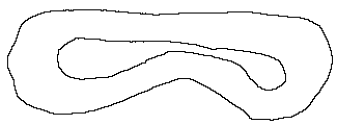
\includegraphics[interpolate=true,width=3.370000in,height=1.250000in]{contents/chapt6/figs/steer/lfc_paths-img0.png}}%
\end{pgfscope}%
\begin{pgfscope}%
\pgfpathrectangle{\pgfqpoint{1.188281in}{2.512600in}}{\pgfqpoint{3.364627in}{1.242324in}}%
\pgfusepath{clip}%
\pgfsetbuttcap%
\pgfsetroundjoin%
\pgfsetlinewidth{1.505625pt}%
\definecolor{currentstroke}{rgb}{0.501961,0.501961,0.501961}%
\pgfsetstrokecolor{currentstroke}%
\pgfsetdash{{5.550000pt}{2.400000pt}}{0.000000pt}%
\pgfpathmoveto{\pgfqpoint{3.050862in}{3.106006in}}%
\pgfpathlineto{\pgfqpoint{3.151999in}{3.083823in}}%
\pgfpathlineto{\pgfqpoint{3.212206in}{3.068515in}}%
\pgfpathlineto{\pgfqpoint{3.271753in}{3.050448in}}%
\pgfpathlineto{\pgfqpoint{3.310921in}{3.036504in}}%
\pgfpathlineto{\pgfqpoint{3.349490in}{3.020992in}}%
\pgfpathlineto{\pgfqpoint{3.387304in}{3.003888in}}%
\pgfpathlineto{\pgfqpoint{3.424208in}{2.985171in}}%
\pgfpathlineto{\pgfqpoint{3.460051in}{2.964818in}}%
\pgfpathlineto{\pgfqpoint{3.494792in}{2.942798in}}%
\pgfpathlineto{\pgfqpoint{3.528498in}{2.919068in}}%
\pgfpathlineto{\pgfqpoint{3.561239in}{2.893584in}}%
\pgfpathlineto{\pgfqpoint{3.593086in}{2.866306in}}%
\pgfpathlineto{\pgfqpoint{3.639469in}{2.822283in}}%
\pgfpathlineto{\pgfqpoint{3.685996in}{2.778603in}}%
\pgfpathlineto{\pgfqpoint{3.718466in}{2.752904in}}%
\pgfpathlineto{\pgfqpoint{3.735447in}{2.741813in}}%
\pgfpathlineto{\pgfqpoint{3.753063in}{2.732219in}}%
\pgfpathlineto{\pgfqpoint{3.771419in}{2.724367in}}%
\pgfpathlineto{\pgfqpoint{3.790561in}{2.718409in}}%
\pgfpathlineto{\pgfqpoint{3.810387in}{2.714264in}}%
\pgfpathlineto{\pgfqpoint{3.830774in}{2.711812in}}%
\pgfpathlineto{\pgfqpoint{3.851597in}{2.710934in}}%
\pgfpathlineto{\pgfqpoint{3.872730in}{2.711509in}}%
\pgfpathlineto{\pgfqpoint{3.894049in}{2.713418in}}%
\pgfpathlineto{\pgfqpoint{3.936746in}{2.720758in}}%
\pgfpathlineto{\pgfqpoint{3.978689in}{2.731996in}}%
\pgfpathlineto{\pgfqpoint{4.019024in}{2.746433in}}%
\pgfpathlineto{\pgfqpoint{4.057299in}{2.764101in}}%
\pgfpathlineto{\pgfqpoint{4.093131in}{2.785158in}}%
\pgfpathlineto{\pgfqpoint{4.110012in}{2.797007in}}%
\pgfpathlineto{\pgfqpoint{4.126139in}{2.809762in}}%
\pgfpathlineto{\pgfqpoint{4.141464in}{2.823444in}}%
\pgfpathlineto{\pgfqpoint{4.155939in}{2.838069in}}%
\pgfpathlineto{\pgfqpoint{4.169529in}{2.853618in}}%
\pgfpathlineto{\pgfqpoint{4.182212in}{2.870022in}}%
\pgfpathlineto{\pgfqpoint{4.193964in}{2.887213in}}%
\pgfpathlineto{\pgfqpoint{4.204764in}{2.905121in}}%
\pgfpathlineto{\pgfqpoint{4.214590in}{2.923676in}}%
\pgfpathlineto{\pgfqpoint{4.223419in}{2.942811in}}%
\pgfpathlineto{\pgfqpoint{4.231229in}{2.962454in}}%
\pgfpathlineto{\pgfqpoint{4.237999in}{2.982538in}}%
\pgfpathlineto{\pgfqpoint{4.243705in}{3.002992in}}%
\pgfpathlineto{\pgfqpoint{4.248325in}{3.023748in}}%
\pgfpathlineto{\pgfqpoint{4.251825in}{3.044725in}}%
\pgfpathlineto{\pgfqpoint{4.254156in}{3.065837in}}%
\pgfpathlineto{\pgfqpoint{4.255270in}{3.086995in}}%
\pgfpathlineto{\pgfqpoint{4.255118in}{3.108109in}}%
\pgfpathlineto{\pgfqpoint{4.253652in}{3.129092in}}%
\pgfpathlineto{\pgfqpoint{4.250823in}{3.149855in}}%
\pgfpathlineto{\pgfqpoint{4.246583in}{3.170308in}}%
\pgfpathlineto{\pgfqpoint{4.240882in}{3.190365in}}%
\pgfpathlineto{\pgfqpoint{4.233673in}{3.209934in}}%
\pgfpathlineto{\pgfqpoint{4.224916in}{3.228930in}}%
\pgfpathlineto{\pgfqpoint{4.214664in}{3.247268in}}%
\pgfpathlineto{\pgfqpoint{4.203026in}{3.264866in}}%
\pgfpathlineto{\pgfqpoint{4.190111in}{3.281645in}}%
\pgfpathlineto{\pgfqpoint{4.176031in}{3.297523in}}%
\pgfpathlineto{\pgfqpoint{4.160893in}{3.312419in}}%
\pgfpathlineto{\pgfqpoint{4.144809in}{3.326252in}}%
\pgfpathlineto{\pgfqpoint{4.127887in}{3.338941in}}%
\pgfpathlineto{\pgfqpoint{4.110238in}{3.350406in}}%
\pgfpathlineto{\pgfqpoint{4.091970in}{3.360565in}}%
\pgfpathlineto{\pgfqpoint{4.073188in}{3.369367in}}%
\pgfpathlineto{\pgfqpoint{4.053961in}{3.376912in}}%
\pgfpathlineto{\pgfqpoint{4.014399in}{3.388843in}}%
\pgfpathlineto{\pgfqpoint{3.973748in}{3.397573in}}%
\pgfpathlineto{\pgfqpoint{3.911738in}{3.407324in}}%
\pgfpathlineto{\pgfqpoint{3.686000in}{3.439363in}}%
\pgfpathlineto{\pgfqpoint{3.624214in}{3.444354in}}%
\pgfpathlineto{\pgfqpoint{3.562130in}{3.447073in}}%
\pgfpathlineto{\pgfqpoint{3.479138in}{3.448054in}}%
\pgfpathlineto{\pgfqpoint{3.313386in}{3.448023in}}%
\pgfpathlineto{\pgfqpoint{3.251467in}{3.451103in}}%
\pgfpathlineto{\pgfqpoint{3.189691in}{3.456926in}}%
\pgfpathlineto{\pgfqpoint{2.963087in}{3.482224in}}%
\pgfpathlineto{\pgfqpoint{2.901097in}{3.486031in}}%
\pgfpathlineto{\pgfqpoint{2.839064in}{3.487479in}}%
\pgfpathlineto{\pgfqpoint{2.777004in}{3.486661in}}%
\pgfpathlineto{\pgfqpoint{2.528391in}{3.480271in}}%
\pgfpathlineto{\pgfqpoint{2.466348in}{3.482502in}}%
\pgfpathlineto{\pgfqpoint{2.404508in}{3.487775in}}%
\pgfpathlineto{\pgfqpoint{2.219191in}{3.507483in}}%
\pgfpathlineto{\pgfqpoint{2.157089in}{3.509602in}}%
\pgfpathlineto{\pgfqpoint{2.094910in}{3.509391in}}%
\pgfpathlineto{\pgfqpoint{2.012136in}{3.506922in}}%
\pgfpathlineto{\pgfqpoint{1.950248in}{3.503652in}}%
\pgfpathlineto{\pgfqpoint{1.888437in}{3.497884in}}%
\pgfpathlineto{\pgfqpoint{1.847224in}{3.491982in}}%
\pgfpathlineto{\pgfqpoint{1.806005in}{3.483959in}}%
\pgfpathlineto{\pgfqpoint{1.765209in}{3.473312in}}%
\pgfpathlineto{\pgfqpoint{1.725566in}{3.459471in}}%
\pgfpathlineto{\pgfqpoint{1.706406in}{3.451174in}}%
\pgfpathlineto{\pgfqpoint{1.687809in}{3.441864in}}%
\pgfpathlineto{\pgfqpoint{1.669867in}{3.431469in}}%
\pgfpathlineto{\pgfqpoint{1.652673in}{3.419919in}}%
\pgfpathlineto{\pgfqpoint{1.636318in}{3.407142in}}%
\pgfpathlineto{\pgfqpoint{1.620878in}{3.393130in}}%
\pgfpathlineto{\pgfqpoint{1.606406in}{3.377979in}}%
\pgfpathlineto{\pgfqpoint{1.592953in}{3.361796in}}%
\pgfpathlineto{\pgfqpoint{1.580568in}{3.344688in}}%
\pgfpathlineto{\pgfqpoint{1.569301in}{3.326762in}}%
\pgfpathlineto{\pgfqpoint{1.559202in}{3.308123in}}%
\pgfpathlineto{\pgfqpoint{1.550322in}{3.288880in}}%
\pgfpathlineto{\pgfqpoint{1.542710in}{3.269138in}}%
\pgfpathlineto{\pgfqpoint{1.536416in}{3.249005in}}%
\pgfpathlineto{\pgfqpoint{1.531489in}{3.228586in}}%
\pgfpathlineto{\pgfqpoint{1.527945in}{3.207967in}}%
\pgfpathlineto{\pgfqpoint{1.525753in}{3.187203in}}%
\pgfpathlineto{\pgfqpoint{1.524882in}{3.166351in}}%
\pgfpathlineto{\pgfqpoint{1.525300in}{3.145465in}}%
\pgfpathlineto{\pgfqpoint{1.526973in}{3.124600in}}%
\pgfpathlineto{\pgfqpoint{1.529869in}{3.103811in}}%
\pgfpathlineto{\pgfqpoint{1.533956in}{3.083153in}}%
\pgfpathlineto{\pgfqpoint{1.539202in}{3.062681in}}%
\pgfpathlineto{\pgfqpoint{1.545573in}{3.042450in}}%
\pgfpathlineto{\pgfqpoint{1.553039in}{3.022518in}}%
\pgfpathlineto{\pgfqpoint{1.561573in}{3.002970in}}%
\pgfpathlineto{\pgfqpoint{1.571155in}{2.983919in}}%
\pgfpathlineto{\pgfqpoint{1.581764in}{2.965475in}}%
\pgfpathlineto{\pgfqpoint{1.593380in}{2.947749in}}%
\pgfpathlineto{\pgfqpoint{1.605982in}{2.930851in}}%
\pgfpathlineto{\pgfqpoint{1.619550in}{2.914892in}}%
\pgfpathlineto{\pgfqpoint{1.634063in}{2.899983in}}%
\pgfpathlineto{\pgfqpoint{1.649501in}{2.886236in}}%
\pgfpathlineto{\pgfqpoint{1.665843in}{2.873761in}}%
\pgfpathlineto{\pgfqpoint{1.683061in}{2.862649in}}%
\pgfpathlineto{\pgfqpoint{1.701080in}{2.852857in}}%
\pgfpathlineto{\pgfqpoint{1.719807in}{2.844287in}}%
\pgfpathlineto{\pgfqpoint{1.739144in}{2.836839in}}%
\pgfpathlineto{\pgfqpoint{1.779272in}{2.824912in}}%
\pgfpathlineto{\pgfqpoint{1.820705in}{2.816285in}}%
\pgfpathlineto{\pgfqpoint{1.862681in}{2.810163in}}%
\pgfpathlineto{\pgfqpoint{1.904553in}{2.805891in}}%
\pgfpathlineto{\pgfqpoint{1.946187in}{2.803433in}}%
\pgfpathlineto{\pgfqpoint{1.987591in}{2.802926in}}%
\pgfpathlineto{\pgfqpoint{2.028774in}{2.804510in}}%
\pgfpathlineto{\pgfqpoint{2.069744in}{2.808323in}}%
\pgfpathlineto{\pgfqpoint{2.110511in}{2.814409in}}%
\pgfpathlineto{\pgfqpoint{2.151079in}{2.822450in}}%
\pgfpathlineto{\pgfqpoint{2.211571in}{2.837295in}}%
\pgfpathlineto{\pgfqpoint{2.291578in}{2.860170in}}%
\pgfpathlineto{\pgfqpoint{2.370741in}{2.885006in}}%
\pgfpathlineto{\pgfqpoint{2.429342in}{2.905383in}}%
\pgfpathlineto{\pgfqpoint{2.487103in}{2.927760in}}%
\pgfpathlineto{\pgfqpoint{2.544060in}{2.952175in}}%
\pgfpathlineto{\pgfqpoint{2.619283in}{2.987005in}}%
\pgfpathlineto{\pgfqpoint{2.751276in}{3.048974in}}%
\pgfpathlineto{\pgfqpoint{2.789731in}{3.064339in}}%
\pgfpathlineto{\pgfqpoint{2.828797in}{3.077384in}}%
\pgfpathlineto{\pgfqpoint{2.868618in}{3.087451in}}%
\pgfpathlineto{\pgfqpoint{2.909168in}{3.094608in}}%
\pgfpathlineto{\pgfqpoint{2.950281in}{3.099509in}}%
\pgfpathlineto{\pgfqpoint{3.012644in}{3.104098in}}%
\pgfpathlineto{\pgfqpoint{3.033532in}{3.105226in}}%
\pgfpathlineto{\pgfqpoint{3.033532in}{3.105226in}}%
\pgfusepath{stroke}%
\end{pgfscope}%
\begin{pgfscope}%
\pgfpathrectangle{\pgfqpoint{1.188281in}{2.512600in}}{\pgfqpoint{3.364627in}{1.242324in}}%
\pgfusepath{clip}%
\pgfsetrectcap%
\pgfsetroundjoin%
\pgfsetlinewidth{1.505625pt}%
\definecolor{currentstroke}{rgb}{0.121569,0.466667,0.705882}%
\pgfsetstrokecolor{currentstroke}%
\pgfsetstrokeopacity{0.800000}%
\pgfsetdash{}{0pt}%
\pgfpathmoveto{\pgfqpoint{3.258821in}{3.444343in}}%
\pgfpathlineto{\pgfqpoint{3.140103in}{3.445291in}}%
\pgfpathlineto{\pgfqpoint{3.055496in}{3.448203in}}%
\pgfpathlineto{\pgfqpoint{2.983364in}{3.453073in}}%
\pgfpathlineto{\pgfqpoint{2.921403in}{3.459725in}}%
\pgfpathlineto{\pgfqpoint{2.870088in}{3.467689in}}%
\pgfpathlineto{\pgfqpoint{2.798794in}{3.481948in}}%
\pgfpathlineto{\pgfqpoint{2.717207in}{3.497682in}}%
\pgfpathlineto{\pgfqpoint{2.665806in}{3.505066in}}%
\pgfpathlineto{\pgfqpoint{2.603773in}{3.511029in}}%
\pgfpathlineto{\pgfqpoint{2.448548in}{3.524308in}}%
\pgfpathlineto{\pgfqpoint{2.303954in}{3.539704in}}%
\pgfpathlineto{\pgfqpoint{2.241764in}{3.543696in}}%
\pgfpathlineto{\pgfqpoint{2.179466in}{3.545245in}}%
\pgfpathlineto{\pgfqpoint{2.117156in}{3.544292in}}%
\pgfpathlineto{\pgfqpoint{2.054928in}{3.540949in}}%
\pgfpathlineto{\pgfqpoint{2.003251in}{3.535835in}}%
\pgfpathlineto{\pgfqpoint{1.962165in}{3.529685in}}%
\pgfpathlineto{\pgfqpoint{1.921482in}{3.521284in}}%
\pgfpathlineto{\pgfqpoint{1.881439in}{3.510232in}}%
\pgfpathlineto{\pgfqpoint{1.851991in}{3.500055in}}%
\pgfpathlineto{\pgfqpoint{1.823230in}{3.488077in}}%
\pgfpathlineto{\pgfqpoint{1.795462in}{3.473955in}}%
\pgfpathlineto{\pgfqpoint{1.768959in}{3.457582in}}%
\pgfpathlineto{\pgfqpoint{1.744036in}{3.438896in}}%
\pgfpathlineto{\pgfqpoint{1.721108in}{3.417813in}}%
\pgfpathlineto{\pgfqpoint{1.707120in}{3.402458in}}%
\pgfpathlineto{\pgfqpoint{1.694302in}{3.386115in}}%
\pgfpathlineto{\pgfqpoint{1.682763in}{3.368845in}}%
\pgfpathlineto{\pgfqpoint{1.672519in}{3.350776in}}%
\pgfpathlineto{\pgfqpoint{1.663631in}{3.332003in}}%
\pgfpathlineto{\pgfqpoint{1.656160in}{3.312623in}}%
\pgfpathlineto{\pgfqpoint{1.650172in}{3.292735in}}%
\pgfpathlineto{\pgfqpoint{1.645714in}{3.272449in}}%
\pgfpathlineto{\pgfqpoint{1.642799in}{3.251885in}}%
\pgfpathlineto{\pgfqpoint{1.641438in}{3.231160in}}%
\pgfpathlineto{\pgfqpoint{1.641639in}{3.210391in}}%
\pgfpathlineto{\pgfqpoint{1.643402in}{3.189696in}}%
\pgfpathlineto{\pgfqpoint{1.646783in}{3.169203in}}%
\pgfpathlineto{\pgfqpoint{1.651698in}{3.149023in}}%
\pgfpathlineto{\pgfqpoint{1.658193in}{3.129294in}}%
\pgfpathlineto{\pgfqpoint{1.666233in}{3.110144in}}%
\pgfpathlineto{\pgfqpoint{1.675805in}{3.091712in}}%
\pgfpathlineto{\pgfqpoint{1.686854in}{3.074125in}}%
\pgfpathlineto{\pgfqpoint{1.699323in}{3.057516in}}%
\pgfpathlineto{\pgfqpoint{1.713164in}{3.042030in}}%
\pgfpathlineto{\pgfqpoint{1.728286in}{3.027794in}}%
\pgfpathlineto{\pgfqpoint{1.744590in}{3.014929in}}%
\pgfpathlineto{\pgfqpoint{1.761945in}{3.003521in}}%
\pgfpathlineto{\pgfqpoint{1.780172in}{2.993562in}}%
\pgfpathlineto{\pgfqpoint{1.799103in}{2.985017in}}%
\pgfpathlineto{\pgfqpoint{1.828486in}{2.974675in}}%
\pgfpathlineto{\pgfqpoint{1.858651in}{2.966886in}}%
\pgfpathlineto{\pgfqpoint{1.899512in}{2.959407in}}%
\pgfpathlineto{\pgfqpoint{1.951064in}{2.953157in}}%
\pgfpathlineto{\pgfqpoint{2.002839in}{2.949134in}}%
\pgfpathlineto{\pgfqpoint{2.054738in}{2.947360in}}%
\pgfpathlineto{\pgfqpoint{2.096280in}{2.947858in}}%
\pgfpathlineto{\pgfqpoint{2.137745in}{2.950407in}}%
\pgfpathlineto{\pgfqpoint{2.179028in}{2.955056in}}%
\pgfpathlineto{\pgfqpoint{2.250887in}{2.966123in}}%
\pgfpathlineto{\pgfqpoint{2.333031in}{2.978631in}}%
\pgfpathlineto{\pgfqpoint{2.384663in}{2.984198in}}%
\pgfpathlineto{\pgfqpoint{2.508754in}{2.995674in}}%
\pgfpathlineto{\pgfqpoint{2.539446in}{3.001033in}}%
\pgfpathlineto{\pgfqpoint{2.569734in}{3.008336in}}%
\pgfpathlineto{\pgfqpoint{2.599413in}{3.017808in}}%
\pgfpathlineto{\pgfqpoint{2.628361in}{3.029328in}}%
\pgfpathlineto{\pgfqpoint{2.665801in}{3.047323in}}%
\pgfpathlineto{\pgfqpoint{2.711278in}{3.072396in}}%
\pgfpathlineto{\pgfqpoint{2.819031in}{3.134030in}}%
\pgfpathlineto{\pgfqpoint{2.846850in}{3.147129in}}%
\pgfpathlineto{\pgfqpoint{2.875434in}{3.158116in}}%
\pgfpathlineto{\pgfqpoint{2.904746in}{3.166540in}}%
\pgfpathlineto{\pgfqpoint{2.934643in}{3.171892in}}%
\pgfpathlineto{\pgfqpoint{2.954930in}{3.173592in}}%
\pgfpathlineto{\pgfqpoint{2.985789in}{3.173409in}}%
\pgfpathlineto{\pgfqpoint{3.016757in}{3.170278in}}%
\pgfpathlineto{\pgfqpoint{3.047353in}{3.164554in}}%
\pgfpathlineto{\pgfqpoint{3.077404in}{3.156437in}}%
\pgfpathlineto{\pgfqpoint{3.106752in}{3.146062in}}%
\pgfpathlineto{\pgfqpoint{3.135282in}{3.133610in}}%
\pgfpathlineto{\pgfqpoint{3.162849in}{3.119149in}}%
\pgfpathlineto{\pgfqpoint{3.198183in}{3.097374in}}%
\pgfpathlineto{\pgfqpoint{3.240657in}{3.067572in}}%
\pgfpathlineto{\pgfqpoint{3.308270in}{3.019398in}}%
\pgfpathlineto{\pgfqpoint{3.343342in}{2.997195in}}%
\pgfpathlineto{\pgfqpoint{3.379435in}{2.976693in}}%
\pgfpathlineto{\pgfqpoint{3.443931in}{2.943262in}}%
\pgfpathlineto{\pgfqpoint{3.517388in}{2.904575in}}%
\pgfpathlineto{\pgfqpoint{3.699432in}{2.804903in}}%
\pgfpathlineto{\pgfqpoint{3.737008in}{2.787268in}}%
\pgfpathlineto{\pgfqpoint{3.765879in}{2.775623in}}%
\pgfpathlineto{\pgfqpoint{3.795481in}{2.766000in}}%
\pgfpathlineto{\pgfqpoint{3.825832in}{2.759108in}}%
\pgfpathlineto{\pgfqpoint{3.846394in}{2.756306in}}%
\pgfpathlineto{\pgfqpoint{3.867113in}{2.755125in}}%
\pgfpathlineto{\pgfqpoint{3.887857in}{2.755696in}}%
\pgfpathlineto{\pgfqpoint{3.908477in}{2.758025in}}%
\pgfpathlineto{\pgfqpoint{3.928830in}{2.762074in}}%
\pgfpathlineto{\pgfqpoint{3.948751in}{2.767884in}}%
\pgfpathlineto{\pgfqpoint{3.968073in}{2.775453in}}%
\pgfpathlineto{\pgfqpoint{3.986643in}{2.784714in}}%
\pgfpathlineto{\pgfqpoint{4.004321in}{2.795581in}}%
\pgfpathlineto{\pgfqpoint{4.020977in}{2.807957in}}%
\pgfpathlineto{\pgfqpoint{4.036494in}{2.821736in}}%
\pgfpathlineto{\pgfqpoint{4.050716in}{2.836847in}}%
\pgfpathlineto{\pgfqpoint{4.063541in}{2.853161in}}%
\pgfpathlineto{\pgfqpoint{4.074921in}{2.870514in}}%
\pgfpathlineto{\pgfqpoint{4.084707in}{2.888813in}}%
\pgfpathlineto{\pgfqpoint{4.092882in}{2.907886in}}%
\pgfpathlineto{\pgfqpoint{4.099319in}{2.927614in}}%
\pgfpathlineto{\pgfqpoint{4.103969in}{2.947838in}}%
\pgfpathlineto{\pgfqpoint{4.106792in}{2.968396in}}%
\pgfpathlineto{\pgfqpoint{4.107757in}{2.989125in}}%
\pgfpathlineto{\pgfqpoint{4.106850in}{3.009857in}}%
\pgfpathlineto{\pgfqpoint{4.104037in}{3.030416in}}%
\pgfpathlineto{\pgfqpoint{4.099341in}{3.050629in}}%
\pgfpathlineto{\pgfqpoint{4.092911in}{3.070359in}}%
\pgfpathlineto{\pgfqpoint{4.084897in}{3.089502in}}%
\pgfpathlineto{\pgfqpoint{4.075434in}{3.107971in}}%
\pgfpathlineto{\pgfqpoint{4.064551in}{3.125641in}}%
\pgfpathlineto{\pgfqpoint{4.052369in}{3.142442in}}%
\pgfpathlineto{\pgfqpoint{4.031907in}{3.165892in}}%
\pgfpathlineto{\pgfqpoint{4.009063in}{3.187028in}}%
\pgfpathlineto{\pgfqpoint{3.984164in}{3.205699in}}%
\pgfpathlineto{\pgfqpoint{3.957606in}{3.221932in}}%
\pgfpathlineto{\pgfqpoint{3.929824in}{3.235974in}}%
\pgfpathlineto{\pgfqpoint{3.891529in}{3.251978in}}%
\pgfpathlineto{\pgfqpoint{3.832907in}{3.272968in}}%
\pgfpathlineto{\pgfqpoint{3.745034in}{3.304622in}}%
\pgfpathlineto{\pgfqpoint{3.667082in}{3.333187in}}%
\pgfpathlineto{\pgfqpoint{3.627484in}{3.345637in}}%
\pgfpathlineto{\pgfqpoint{3.587270in}{3.355915in}}%
\pgfpathlineto{\pgfqpoint{3.546514in}{3.363782in}}%
\pgfpathlineto{\pgfqpoint{3.505419in}{3.369629in}}%
\pgfpathlineto{\pgfqpoint{3.464104in}{3.373641in}}%
\pgfpathlineto{\pgfqpoint{3.412292in}{3.376437in}}%
\pgfpathlineto{\pgfqpoint{3.350033in}{3.377453in}}%
\pgfpathlineto{\pgfqpoint{3.256631in}{3.377994in}}%
\pgfpathlineto{\pgfqpoint{3.256631in}{3.377994in}}%
\pgfusepath{stroke}%
\end{pgfscope}%
\begin{pgfscope}%
\pgfpathrectangle{\pgfqpoint{1.188281in}{2.512600in}}{\pgfqpoint{3.364627in}{1.242324in}}%
\pgfusepath{clip}%
\pgfsetrectcap%
\pgfsetroundjoin%
\pgfsetlinewidth{1.505625pt}%
\definecolor{currentstroke}{rgb}{1.000000,0.498039,0.054902}%
\pgfsetstrokecolor{currentstroke}%
\pgfsetstrokeopacity{0.800000}%
\pgfsetdash{}{0pt}%
\pgfpathmoveto{\pgfqpoint{3.258821in}{3.444343in}}%
\pgfpathlineto{\pgfqpoint{3.197933in}{3.443492in}}%
\pgfpathlineto{\pgfqpoint{3.142903in}{3.440199in}}%
\pgfpathlineto{\pgfqpoint{3.090605in}{3.434737in}}%
\pgfpathlineto{\pgfqpoint{2.949122in}{3.416703in}}%
\pgfpathlineto{\pgfqpoint{2.908917in}{3.414782in}}%
\pgfpathlineto{\pgfqpoint{2.867938in}{3.415202in}}%
\pgfpathlineto{\pgfqpoint{2.826531in}{3.417624in}}%
\pgfpathlineto{\pgfqpoint{2.774938in}{3.423187in}}%
\pgfpathlineto{\pgfqpoint{2.723707in}{3.431447in}}%
\pgfpathlineto{\pgfqpoint{2.672918in}{3.442100in}}%
\pgfpathlineto{\pgfqpoint{2.480569in}{3.485517in}}%
\pgfpathlineto{\pgfqpoint{2.419162in}{3.495883in}}%
\pgfpathlineto{\pgfqpoint{2.357455in}{3.504267in}}%
\pgfpathlineto{\pgfqpoint{2.295504in}{3.510608in}}%
\pgfpathlineto{\pgfqpoint{2.233370in}{3.514782in}}%
\pgfpathlineto{\pgfqpoint{2.181495in}{3.516201in}}%
\pgfpathlineto{\pgfqpoint{2.129606in}{3.515484in}}%
\pgfpathlineto{\pgfqpoint{2.077802in}{3.512438in}}%
\pgfpathlineto{\pgfqpoint{2.036526in}{3.508007in}}%
\pgfpathlineto{\pgfqpoint{2.005799in}{3.502979in}}%
\pgfpathlineto{\pgfqpoint{1.975400in}{3.496251in}}%
\pgfpathlineto{\pgfqpoint{1.945488in}{3.487618in}}%
\pgfpathlineto{\pgfqpoint{1.916298in}{3.476796in}}%
\pgfpathlineto{\pgfqpoint{1.888071in}{3.463665in}}%
\pgfpathlineto{\pgfqpoint{1.861015in}{3.448266in}}%
\pgfpathlineto{\pgfqpoint{1.835218in}{3.430837in}}%
\pgfpathlineto{\pgfqpoint{1.810791in}{3.411537in}}%
\pgfpathlineto{\pgfqpoint{1.787818in}{3.390524in}}%
\pgfpathlineto{\pgfqpoint{1.766313in}{3.368011in}}%
\pgfpathlineto{\pgfqpoint{1.746341in}{3.344127in}}%
\pgfpathlineto{\pgfqpoint{1.727975in}{3.318988in}}%
\pgfpathlineto{\pgfqpoint{1.711435in}{3.292613in}}%
\pgfpathlineto{\pgfqpoint{1.697182in}{3.264938in}}%
\pgfpathlineto{\pgfqpoint{1.685598in}{3.236046in}}%
\pgfpathlineto{\pgfqpoint{1.677040in}{3.206121in}}%
\pgfpathlineto{\pgfqpoint{1.673193in}{3.185725in}}%
\pgfpathlineto{\pgfqpoint{1.670918in}{3.165095in}}%
\pgfpathlineto{\pgfqpoint{1.670266in}{3.144350in}}%
\pgfpathlineto{\pgfqpoint{1.671291in}{3.123620in}}%
\pgfpathlineto{\pgfqpoint{1.673919in}{3.103032in}}%
\pgfpathlineto{\pgfqpoint{1.678130in}{3.082708in}}%
\pgfpathlineto{\pgfqpoint{1.683898in}{3.062770in}}%
\pgfpathlineto{\pgfqpoint{1.691170in}{3.043330in}}%
\pgfpathlineto{\pgfqpoint{1.699911in}{3.024505in}}%
\pgfpathlineto{\pgfqpoint{1.710070in}{3.006406in}}%
\pgfpathlineto{\pgfqpoint{1.721570in}{2.989128in}}%
\pgfpathlineto{\pgfqpoint{1.734338in}{2.972765in}}%
\pgfpathlineto{\pgfqpoint{1.748300in}{2.957407in}}%
\pgfpathlineto{\pgfqpoint{1.763376in}{2.943143in}}%
\pgfpathlineto{\pgfqpoint{1.787835in}{2.923892in}}%
\pgfpathlineto{\pgfqpoint{1.814053in}{2.907109in}}%
\pgfpathlineto{\pgfqpoint{1.841610in}{2.892626in}}%
\pgfpathlineto{\pgfqpoint{1.870252in}{2.880428in}}%
\pgfpathlineto{\pgfqpoint{1.899730in}{2.870412in}}%
\pgfpathlineto{\pgfqpoint{1.929817in}{2.862405in}}%
\pgfpathlineto{\pgfqpoint{1.960343in}{2.856280in}}%
\pgfpathlineto{\pgfqpoint{2.001433in}{2.850363in}}%
\pgfpathlineto{\pgfqpoint{2.042766in}{2.846477in}}%
\pgfpathlineto{\pgfqpoint{2.094591in}{2.843805in}}%
\pgfpathlineto{\pgfqpoint{2.156861in}{2.843130in}}%
\pgfpathlineto{\pgfqpoint{2.208736in}{2.844582in}}%
\pgfpathlineto{\pgfqpoint{2.260517in}{2.848011in}}%
\pgfpathlineto{\pgfqpoint{2.312104in}{2.853647in}}%
\pgfpathlineto{\pgfqpoint{2.363378in}{2.861641in}}%
\pgfpathlineto{\pgfqpoint{2.414264in}{2.871820in}}%
\pgfpathlineto{\pgfqpoint{2.464702in}{2.884029in}}%
\pgfpathlineto{\pgfqpoint{2.524598in}{2.901070in}}%
\pgfpathlineto{\pgfqpoint{2.583782in}{2.920445in}}%
\pgfpathlineto{\pgfqpoint{2.671617in}{2.952244in}}%
\pgfpathlineto{\pgfqpoint{2.866238in}{3.024384in}}%
\pgfpathlineto{\pgfqpoint{2.906091in}{3.036012in}}%
\pgfpathlineto{\pgfqpoint{2.946479in}{3.045614in}}%
\pgfpathlineto{\pgfqpoint{2.987364in}{3.052788in}}%
\pgfpathlineto{\pgfqpoint{3.018335in}{3.055963in}}%
\pgfpathlineto{\pgfqpoint{3.049452in}{3.056973in}}%
\pgfpathlineto{\pgfqpoint{3.080551in}{3.055587in}}%
\pgfpathlineto{\pgfqpoint{3.111419in}{3.051555in}}%
\pgfpathlineto{\pgfqpoint{3.141803in}{3.044786in}}%
\pgfpathlineto{\pgfqpoint{3.171421in}{3.035204in}}%
\pgfpathlineto{\pgfqpoint{3.200107in}{3.023111in}}%
\pgfpathlineto{\pgfqpoint{3.227827in}{3.008935in}}%
\pgfpathlineto{\pgfqpoint{3.263460in}{2.987641in}}%
\pgfpathlineto{\pgfqpoint{3.297836in}{2.964365in}}%
\pgfpathlineto{\pgfqpoint{3.347936in}{2.927376in}}%
\pgfpathlineto{\pgfqpoint{3.406429in}{2.884285in}}%
\pgfpathlineto{\pgfqpoint{3.440965in}{2.861248in}}%
\pgfpathlineto{\pgfqpoint{3.476700in}{2.840122in}}%
\pgfpathlineto{\pgfqpoint{3.504378in}{2.825862in}}%
\pgfpathlineto{\pgfqpoint{3.542412in}{2.809233in}}%
\pgfpathlineto{\pgfqpoint{3.581368in}{2.794884in}}%
\pgfpathlineto{\pgfqpoint{3.630792in}{2.779064in}}%
\pgfpathlineto{\pgfqpoint{3.720632in}{2.753470in}}%
\pgfpathlineto{\pgfqpoint{3.780980in}{2.738108in}}%
\pgfpathlineto{\pgfqpoint{3.821746in}{2.730284in}}%
\pgfpathlineto{\pgfqpoint{3.852673in}{2.726713in}}%
\pgfpathlineto{\pgfqpoint{3.883784in}{2.725644in}}%
\pgfpathlineto{\pgfqpoint{3.914851in}{2.727572in}}%
\pgfpathlineto{\pgfqpoint{3.935374in}{2.730672in}}%
\pgfpathlineto{\pgfqpoint{3.955610in}{2.735287in}}%
\pgfpathlineto{\pgfqpoint{3.975445in}{2.741400in}}%
\pgfpathlineto{\pgfqpoint{3.994726in}{2.749081in}}%
\pgfpathlineto{\pgfqpoint{4.013321in}{2.758300in}}%
\pgfpathlineto{\pgfqpoint{4.031100in}{2.769010in}}%
\pgfpathlineto{\pgfqpoint{4.047935in}{2.781148in}}%
\pgfpathlineto{\pgfqpoint{4.063707in}{2.794639in}}%
\pgfpathlineto{\pgfqpoint{4.078303in}{2.809394in}}%
\pgfpathlineto{\pgfqpoint{4.091616in}{2.825317in}}%
\pgfpathlineto{\pgfqpoint{4.103552in}{2.842296in}}%
\pgfpathlineto{\pgfqpoint{4.114079in}{2.860183in}}%
\pgfpathlineto{\pgfqpoint{4.123067in}{2.878890in}}%
\pgfpathlineto{\pgfqpoint{4.130462in}{2.898283in}}%
\pgfpathlineto{\pgfqpoint{4.136215in}{2.918225in}}%
\pgfpathlineto{\pgfqpoint{4.140288in}{2.938576in}}%
\pgfpathlineto{\pgfqpoint{4.142649in}{2.959196in}}%
\pgfpathlineto{\pgfqpoint{4.143282in}{2.979941in}}%
\pgfpathlineto{\pgfqpoint{4.142179in}{3.000667in}}%
\pgfpathlineto{\pgfqpoint{4.139346in}{3.021227in}}%
\pgfpathlineto{\pgfqpoint{4.134863in}{3.041492in}}%
\pgfpathlineto{\pgfqpoint{4.128755in}{3.061328in}}%
\pgfpathlineto{\pgfqpoint{4.121069in}{3.080607in}}%
\pgfpathlineto{\pgfqpoint{4.111867in}{3.099210in}}%
\pgfpathlineto{\pgfqpoint{4.101218in}{3.117025in}}%
\pgfpathlineto{\pgfqpoint{4.089201in}{3.133948in}}%
\pgfpathlineto{\pgfqpoint{4.075900in}{3.149880in}}%
\pgfpathlineto{\pgfqpoint{4.061401in}{3.164731in}}%
\pgfpathlineto{\pgfqpoint{4.045799in}{3.178418in}}%
\pgfpathlineto{\pgfqpoint{4.029189in}{3.190864in}}%
\pgfpathlineto{\pgfqpoint{4.002659in}{3.207142in}}%
\pgfpathlineto{\pgfqpoint{3.974647in}{3.220720in}}%
\pgfpathlineto{\pgfqpoint{3.945598in}{3.231917in}}%
\pgfpathlineto{\pgfqpoint{3.905899in}{3.244049in}}%
\pgfpathlineto{\pgfqpoint{3.835482in}{3.261944in}}%
\pgfpathlineto{\pgfqpoint{3.735030in}{3.288060in}}%
\pgfpathlineto{\pgfqpoint{3.665377in}{3.308728in}}%
\pgfpathlineto{\pgfqpoint{3.486829in}{3.363694in}}%
\pgfpathlineto{\pgfqpoint{3.426463in}{3.378990in}}%
\pgfpathlineto{\pgfqpoint{3.365626in}{3.392298in}}%
\pgfpathlineto{\pgfqpoint{3.304417in}{3.403768in}}%
\pgfpathlineto{\pgfqpoint{3.253158in}{3.411880in}}%
\pgfpathlineto{\pgfqpoint{3.253158in}{3.411880in}}%
\pgfusepath{stroke}%
\end{pgfscope}%
\begin{pgfscope}%
\pgfpathrectangle{\pgfqpoint{1.188281in}{2.512600in}}{\pgfqpoint{3.364627in}{1.242324in}}%
\pgfusepath{clip}%
\pgfsetrectcap%
\pgfsetroundjoin%
\pgfsetlinewidth{1.505625pt}%
\definecolor{currentstroke}{rgb}{0.172549,0.627451,0.172549}%
\pgfsetstrokecolor{currentstroke}%
\pgfsetstrokeopacity{0.800000}%
\pgfsetdash{}{0pt}%
\pgfpathmoveto{\pgfqpoint{3.258821in}{3.444343in}}%
\pgfpathlineto{\pgfqpoint{3.200200in}{3.445442in}}%
\pgfpathlineto{\pgfqpoint{3.165091in}{3.448404in}}%
\pgfpathlineto{\pgfqpoint{3.128334in}{3.453678in}}%
\pgfpathlineto{\pgfqpoint{3.089995in}{3.461647in}}%
\pgfpathlineto{\pgfqpoint{3.041426in}{3.474234in}}%
\pgfpathlineto{\pgfqpoint{2.981099in}{3.492225in}}%
\pgfpathlineto{\pgfqpoint{2.907258in}{3.516836in}}%
\pgfpathlineto{\pgfqpoint{2.838397in}{3.539394in}}%
\pgfpathlineto{\pgfqpoint{2.798334in}{3.550534in}}%
\pgfpathlineto{\pgfqpoint{2.757747in}{3.559570in}}%
\pgfpathlineto{\pgfqpoint{2.716660in}{3.565951in}}%
\pgfpathlineto{\pgfqpoint{2.675262in}{3.569856in}}%
\pgfpathlineto{\pgfqpoint{2.623336in}{3.572190in}}%
\pgfpathlineto{\pgfqpoint{2.560959in}{3.572446in}}%
\pgfpathlineto{\pgfqpoint{2.436209in}{3.572079in}}%
\pgfpathlineto{\pgfqpoint{2.384285in}{3.574487in}}%
\pgfpathlineto{\pgfqpoint{2.332520in}{3.579196in}}%
\pgfpathlineto{\pgfqpoint{2.281023in}{3.586265in}}%
\pgfpathlineto{\pgfqpoint{2.188409in}{3.599557in}}%
\pgfpathlineto{\pgfqpoint{2.146984in}{3.603159in}}%
\pgfpathlineto{\pgfqpoint{2.115812in}{3.604133in}}%
\pgfpathlineto{\pgfqpoint{2.084642in}{3.603179in}}%
\pgfpathlineto{\pgfqpoint{2.053614in}{3.600067in}}%
\pgfpathlineto{\pgfqpoint{2.022906in}{3.594643in}}%
\pgfpathlineto{\pgfqpoint{1.992700in}{3.586895in}}%
\pgfpathlineto{\pgfqpoint{1.963196in}{3.576805in}}%
\pgfpathlineto{\pgfqpoint{1.934590in}{3.564391in}}%
\pgfpathlineto{\pgfqpoint{1.907060in}{3.549747in}}%
\pgfpathlineto{\pgfqpoint{1.880714in}{3.533066in}}%
\pgfpathlineto{\pgfqpoint{1.855686in}{3.514463in}}%
\pgfpathlineto{\pgfqpoint{1.832073in}{3.494095in}}%
\pgfpathlineto{\pgfqpoint{1.809973in}{3.472094in}}%
\pgfpathlineto{\pgfqpoint{1.789450in}{3.448615in}}%
\pgfpathlineto{\pgfqpoint{1.770590in}{3.423780in}}%
\pgfpathlineto{\pgfqpoint{1.753473in}{3.397714in}}%
\pgfpathlineto{\pgfqpoint{1.738258in}{3.370493in}}%
\pgfpathlineto{\pgfqpoint{1.724929in}{3.342301in}}%
\pgfpathlineto{\pgfqpoint{1.713567in}{3.313260in}}%
\pgfpathlineto{\pgfqpoint{1.704208in}{3.283513in}}%
\pgfpathlineto{\pgfqpoint{1.696903in}{3.253196in}}%
\pgfpathlineto{\pgfqpoint{1.691652in}{3.222456in}}%
\pgfpathlineto{\pgfqpoint{1.688583in}{3.191424in}}%
\pgfpathlineto{\pgfqpoint{1.687991in}{3.160248in}}%
\pgfpathlineto{\pgfqpoint{1.689942in}{3.129127in}}%
\pgfpathlineto{\pgfqpoint{1.694569in}{3.098291in}}%
\pgfpathlineto{\pgfqpoint{1.701953in}{3.067998in}}%
\pgfpathlineto{\pgfqpoint{1.712157in}{3.038536in}}%
\pgfpathlineto{\pgfqpoint{1.725153in}{3.010194in}}%
\pgfpathlineto{\pgfqpoint{1.740778in}{2.983212in}}%
\pgfpathlineto{\pgfqpoint{1.758908in}{2.957846in}}%
\pgfpathlineto{\pgfqpoint{1.779354in}{2.934306in}}%
\pgfpathlineto{\pgfqpoint{1.801858in}{2.912723in}}%
\pgfpathlineto{\pgfqpoint{1.826173in}{2.893203in}}%
\pgfpathlineto{\pgfqpoint{1.852086in}{2.875859in}}%
\pgfpathlineto{\pgfqpoint{1.879331in}{2.860692in}}%
\pgfpathlineto{\pgfqpoint{1.907671in}{2.847682in}}%
\pgfpathlineto{\pgfqpoint{1.936904in}{2.836824in}}%
\pgfpathlineto{\pgfqpoint{1.966815in}{2.828001in}}%
\pgfpathlineto{\pgfqpoint{1.997240in}{2.821157in}}%
\pgfpathlineto{\pgfqpoint{2.028036in}{2.816246in}}%
\pgfpathlineto{\pgfqpoint{2.059072in}{2.813187in}}%
\pgfpathlineto{\pgfqpoint{2.090235in}{2.812012in}}%
\pgfpathlineto{\pgfqpoint{2.121412in}{2.812758in}}%
\pgfpathlineto{\pgfqpoint{2.152485in}{2.815404in}}%
\pgfpathlineto{\pgfqpoint{2.183331in}{2.819988in}}%
\pgfpathlineto{\pgfqpoint{2.213828in}{2.826504in}}%
\pgfpathlineto{\pgfqpoint{2.243847in}{2.834955in}}%
\pgfpathlineto{\pgfqpoint{2.273299in}{2.845207in}}%
\pgfpathlineto{\pgfqpoint{2.311670in}{2.861229in}}%
\pgfpathlineto{\pgfqpoint{2.358613in}{2.883550in}}%
\pgfpathlineto{\pgfqpoint{2.507734in}{2.957234in}}%
\pgfpathlineto{\pgfqpoint{2.555471in}{2.977803in}}%
\pgfpathlineto{\pgfqpoint{2.603894in}{2.996704in}}%
\pgfpathlineto{\pgfqpoint{2.662846in}{3.017084in}}%
\pgfpathlineto{\pgfqpoint{2.712736in}{3.031669in}}%
\pgfpathlineto{\pgfqpoint{2.753138in}{3.041511in}}%
\pgfpathlineto{\pgfqpoint{2.793945in}{3.049504in}}%
\pgfpathlineto{\pgfqpoint{2.835098in}{3.055464in}}%
\pgfpathlineto{\pgfqpoint{2.876511in}{3.059198in}}%
\pgfpathlineto{\pgfqpoint{2.918073in}{3.060434in}}%
\pgfpathlineto{\pgfqpoint{2.959630in}{3.059047in}}%
\pgfpathlineto{\pgfqpoint{3.001003in}{3.054912in}}%
\pgfpathlineto{\pgfqpoint{3.041995in}{3.047948in}}%
\pgfpathlineto{\pgfqpoint{3.082421in}{3.038219in}}%
\pgfpathlineto{\pgfqpoint{3.122250in}{3.026274in}}%
\pgfpathlineto{\pgfqpoint{3.161441in}{3.012374in}}%
\pgfpathlineto{\pgfqpoint{3.209573in}{2.992750in}}%
\pgfpathlineto{\pgfqpoint{3.256828in}{2.971095in}}%
\pgfpathlineto{\pgfqpoint{3.303143in}{2.947499in}}%
\pgfpathlineto{\pgfqpoint{3.348425in}{2.921977in}}%
\pgfpathlineto{\pgfqpoint{3.392536in}{2.894479in}}%
\pgfpathlineto{\pgfqpoint{3.435507in}{2.865232in}}%
\pgfpathlineto{\pgfqpoint{3.546493in}{2.788116in}}%
\pgfpathlineto{\pgfqpoint{3.590739in}{2.760840in}}%
\pgfpathlineto{\pgfqpoint{3.627214in}{2.740874in}}%
\pgfpathlineto{\pgfqpoint{3.655405in}{2.727539in}}%
\pgfpathlineto{\pgfqpoint{3.684335in}{2.715894in}}%
\pgfpathlineto{\pgfqpoint{3.713960in}{2.706156in}}%
\pgfpathlineto{\pgfqpoint{3.744211in}{2.698586in}}%
\pgfpathlineto{\pgfqpoint{3.774955in}{2.693379in}}%
\pgfpathlineto{\pgfqpoint{3.805861in}{2.690725in}}%
\pgfpathlineto{\pgfqpoint{3.836389in}{2.690876in}}%
\pgfpathlineto{\pgfqpoint{3.866269in}{2.693965in}}%
\pgfpathlineto{\pgfqpoint{3.895176in}{2.700099in}}%
\pgfpathlineto{\pgfqpoint{3.922767in}{2.709221in}}%
\pgfpathlineto{\pgfqpoint{3.940250in}{2.716930in}}%
\pgfpathlineto{\pgfqpoint{3.956883in}{2.725887in}}%
\pgfpathlineto{\pgfqpoint{3.972568in}{2.736020in}}%
\pgfpathlineto{\pgfqpoint{3.987599in}{2.747582in}}%
\pgfpathlineto{\pgfqpoint{4.009117in}{2.767472in}}%
\pgfpathlineto{\pgfqpoint{4.029500in}{2.789945in}}%
\pgfpathlineto{\pgfqpoint{4.048829in}{2.814514in}}%
\pgfpathlineto{\pgfqpoint{4.066607in}{2.840367in}}%
\pgfpathlineto{\pgfqpoint{4.082709in}{2.867295in}}%
\pgfpathlineto{\pgfqpoint{4.096928in}{2.895262in}}%
\pgfpathlineto{\pgfqpoint{4.109055in}{2.924198in}}%
\pgfpathlineto{\pgfqpoint{4.118858in}{2.953999in}}%
\pgfpathlineto{\pgfqpoint{4.126177in}{2.984505in}}%
\pgfpathlineto{\pgfqpoint{4.130859in}{3.015526in}}%
\pgfpathlineto{\pgfqpoint{4.132829in}{3.046835in}}%
\pgfpathlineto{\pgfqpoint{4.132014in}{3.078195in}}%
\pgfpathlineto{\pgfqpoint{4.128413in}{3.109359in}}%
\pgfpathlineto{\pgfqpoint{4.122022in}{3.140072in}}%
\pgfpathlineto{\pgfqpoint{4.112899in}{3.170087in}}%
\pgfpathlineto{\pgfqpoint{4.101098in}{3.199153in}}%
\pgfpathlineto{\pgfqpoint{4.086726in}{3.227038in}}%
\pgfpathlineto{\pgfqpoint{4.069884in}{3.253504in}}%
\pgfpathlineto{\pgfqpoint{4.050649in}{3.278285in}}%
\pgfpathlineto{\pgfqpoint{4.029163in}{3.301143in}}%
\pgfpathlineto{\pgfqpoint{4.005665in}{3.321926in}}%
\pgfpathlineto{\pgfqpoint{3.980346in}{3.340447in}}%
\pgfpathlineto{\pgfqpoint{3.953415in}{3.356535in}}%
\pgfpathlineto{\pgfqpoint{3.925119in}{3.370077in}}%
\pgfpathlineto{\pgfqpoint{3.895695in}{3.380957in}}%
\pgfpathlineto{\pgfqpoint{3.865403in}{3.389110in}}%
\pgfpathlineto{\pgfqpoint{3.834496in}{3.394494in}}%
\pgfpathlineto{\pgfqpoint{3.803257in}{3.397399in}}%
\pgfpathlineto{\pgfqpoint{3.771893in}{3.398258in}}%
\pgfpathlineto{\pgfqpoint{3.730069in}{3.397213in}}%
\pgfpathlineto{\pgfqpoint{3.646446in}{3.394332in}}%
\pgfpathlineto{\pgfqpoint{3.604628in}{3.395481in}}%
\pgfpathlineto{\pgfqpoint{3.573381in}{3.398319in}}%
\pgfpathlineto{\pgfqpoint{3.542384in}{3.403173in}}%
\pgfpathlineto{\pgfqpoint{3.511809in}{3.410213in}}%
\pgfpathlineto{\pgfqpoint{3.481818in}{3.419426in}}%
\pgfpathlineto{\pgfqpoint{3.452560in}{3.430752in}}%
\pgfpathlineto{\pgfqpoint{3.424176in}{3.444122in}}%
\pgfpathlineto{\pgfqpoint{3.387619in}{3.464459in}}%
\pgfpathlineto{\pgfqpoint{3.343350in}{3.492303in}}%
\pgfpathlineto{\pgfqpoint{3.290179in}{3.525635in}}%
\pgfpathlineto{\pgfqpoint{3.281131in}{3.530885in}}%
\pgfpathlineto{\pgfqpoint{3.281131in}{3.530885in}}%
\pgfusepath{stroke}%
\end{pgfscope}%
\begin{pgfscope}%
\pgfpathrectangle{\pgfqpoint{1.188281in}{2.512600in}}{\pgfqpoint{3.364627in}{1.242324in}}%
\pgfusepath{clip}%
\pgfsetbuttcap%
\pgfsetroundjoin%
\pgfsetlinewidth{1.505625pt}%
\definecolor{currentstroke}{rgb}{1.000000,0.000000,0.000000}%
\pgfsetstrokecolor{currentstroke}%
\pgfsetdash{{1.500000pt}{2.475000pt}}{0.000000pt}%
\pgfpathmoveto{\pgfqpoint{3.251467in}{3.244049in}}%
\pgfpathlineto{\pgfqpoint{3.251467in}{3.658157in}}%
\pgfusepath{stroke}%
\end{pgfscope}%
\begin{pgfscope}%
\pgfsetbuttcap%
\pgfsetmiterjoin%
\definecolor{currentfill}{rgb}{1.000000,1.000000,1.000000}%
\pgfsetfillcolor{currentfill}%
\pgfsetlinewidth{1.003750pt}%
\definecolor{currentstroke}{rgb}{0.000000,0.000000,0.000000}%
\pgfsetstrokecolor{currentstroke}%
\pgfsetdash{}{0pt}%
\pgfpathmoveto{\pgfqpoint{1.970864in}{3.464136in}}%
\pgfpathlineto{\pgfqpoint{2.225345in}{3.464136in}}%
\pgfpathquadraticcurveto{\pgfqpoint{2.239229in}{3.464136in}}{\pgfqpoint{2.239229in}{3.478020in}}%
\pgfpathlineto{\pgfqpoint{2.239229in}{3.601303in}}%
\pgfpathquadraticcurveto{\pgfqpoint{2.239229in}{3.615187in}}{\pgfqpoint{2.225345in}{3.615187in}}%
\pgfpathlineto{\pgfqpoint{1.970864in}{3.615187in}}%
\pgfpathquadraticcurveto{\pgfqpoint{1.956980in}{3.615187in}}{\pgfqpoint{1.956980in}{3.601303in}}%
\pgfpathlineto{\pgfqpoint{1.956980in}{3.478020in}}%
\pgfpathquadraticcurveto{\pgfqpoint{1.956980in}{3.464136in}}{\pgfqpoint{1.970864in}{3.464136in}}%
\pgfpathlineto{\pgfqpoint{1.970864in}{3.464136in}}%
\pgfpathclose%
\pgfusepath{stroke,fill}%
\end{pgfscope}%
\begin{pgfscope}%
\definecolor{textcolor}{rgb}{0.000000,0.000000,0.000000}%
\pgfsetstrokecolor{textcolor}%
\pgfsetfillcolor{textcolor}%
\pgftext[x=1.970864in,y=3.504953in,left,base]{\color{textcolor}\rmfamily\fontsize{9.996000}{11.995200}\selectfont 20\%}%
\end{pgfscope}%
\begin{pgfscope}%
\pgfsetbuttcap%
\pgfsetmiterjoin%
\definecolor{currentfill}{rgb}{1.000000,1.000000,1.000000}%
\pgfsetfillcolor{currentfill}%
\pgfsetlinewidth{1.003750pt}%
\definecolor{currentstroke}{rgb}{0.000000,0.000000,0.000000}%
\pgfsetstrokecolor{currentstroke}%
\pgfsetdash{}{0pt}%
\pgfpathmoveto{\pgfqpoint{1.966917in}{2.762110in}}%
\pgfpathlineto{\pgfqpoint{2.221399in}{2.762110in}}%
\pgfpathquadraticcurveto{\pgfqpoint{2.235282in}{2.762110in}}{\pgfqpoint{2.235282in}{2.775993in}}%
\pgfpathlineto{\pgfqpoint{2.235282in}{2.899277in}}%
\pgfpathquadraticcurveto{\pgfqpoint{2.235282in}{2.913161in}}{\pgfqpoint{2.221399in}{2.913161in}}%
\pgfpathlineto{\pgfqpoint{1.966917in}{2.913161in}}%
\pgfpathquadraticcurveto{\pgfqpoint{1.953034in}{2.913161in}}{\pgfqpoint{1.953034in}{2.899277in}}%
\pgfpathlineto{\pgfqpoint{1.953034in}{2.775993in}}%
\pgfpathquadraticcurveto{\pgfqpoint{1.953034in}{2.762110in}}{\pgfqpoint{1.966917in}{2.762110in}}%
\pgfpathlineto{\pgfqpoint{1.966917in}{2.762110in}}%
\pgfpathclose%
\pgfusepath{stroke,fill}%
\end{pgfscope}%
\begin{pgfscope}%
\definecolor{textcolor}{rgb}{0.000000,0.000000,0.000000}%
\pgfsetstrokecolor{textcolor}%
\pgfsetfillcolor{textcolor}%
\pgftext[x=1.966917in,y=2.802927in,left,base]{\color{textcolor}\rmfamily\fontsize{9.996000}{11.995200}\selectfont 40\%}%
\end{pgfscope}%
\begin{pgfscope}%
\pgfsetbuttcap%
\pgfsetmiterjoin%
\definecolor{currentfill}{rgb}{1.000000,1.000000,1.000000}%
\pgfsetfillcolor{currentfill}%
\pgfsetlinewidth{1.003750pt}%
\definecolor{currentstroke}{rgb}{0.000000,0.000000,0.000000}%
\pgfsetstrokecolor{currentstroke}%
\pgfsetdash{}{0pt}%
\pgfpathmoveto{\pgfqpoint{3.192198in}{3.033057in}}%
\pgfpathlineto{\pgfqpoint{3.446679in}{3.033057in}}%
\pgfpathquadraticcurveto{\pgfqpoint{3.460563in}{3.033057in}}{\pgfqpoint{3.460563in}{3.046940in}}%
\pgfpathlineto{\pgfqpoint{3.460563in}{3.170224in}}%
\pgfpathquadraticcurveto{\pgfqpoint{3.460563in}{3.184108in}}{\pgfqpoint{3.446679in}{3.184108in}}%
\pgfpathlineto{\pgfqpoint{3.192198in}{3.184108in}}%
\pgfpathquadraticcurveto{\pgfqpoint{3.178314in}{3.184108in}}{\pgfqpoint{3.178314in}{3.170224in}}%
\pgfpathlineto{\pgfqpoint{3.178314in}{3.046940in}}%
\pgfpathquadraticcurveto{\pgfqpoint{3.178314in}{3.033057in}}{\pgfqpoint{3.192198in}{3.033057in}}%
\pgfpathlineto{\pgfqpoint{3.192198in}{3.033057in}}%
\pgfpathclose%
\pgfusepath{stroke,fill}%
\end{pgfscope}%
\begin{pgfscope}%
\definecolor{textcolor}{rgb}{0.000000,0.000000,0.000000}%
\pgfsetstrokecolor{textcolor}%
\pgfsetfillcolor{textcolor}%
\pgftext[x=3.192198in,y=3.073874in,left,base]{\color{textcolor}\rmfamily\fontsize{9.996000}{11.995200}\selectfont 60\%}%
\end{pgfscope}%
\begin{pgfscope}%
\pgfsetbuttcap%
\pgfsetmiterjoin%
\definecolor{currentfill}{rgb}{1.000000,1.000000,1.000000}%
\pgfsetfillcolor{currentfill}%
\pgfsetlinewidth{1.003750pt}%
\definecolor{currentstroke}{rgb}{0.000000,0.000000,0.000000}%
\pgfsetstrokecolor{currentstroke}%
\pgfsetdash{}{0pt}%
\pgfpathmoveto{\pgfqpoint{4.237999in}{2.941721in}}%
\pgfpathlineto{\pgfqpoint{4.492480in}{2.941721in}}%
\pgfpathquadraticcurveto{\pgfqpoint{4.506364in}{2.941721in}}{\pgfqpoint{4.506364in}{2.955604in}}%
\pgfpathlineto{\pgfqpoint{4.506364in}{3.078888in}}%
\pgfpathquadraticcurveto{\pgfqpoint{4.506364in}{3.092772in}}{\pgfqpoint{4.492480in}{3.092772in}}%
\pgfpathlineto{\pgfqpoint{4.237999in}{3.092772in}}%
\pgfpathquadraticcurveto{\pgfqpoint{4.224115in}{3.092772in}}{\pgfqpoint{4.224115in}{3.078888in}}%
\pgfpathlineto{\pgfqpoint{4.224115in}{2.955604in}}%
\pgfpathquadraticcurveto{\pgfqpoint{4.224115in}{2.941721in}}{\pgfqpoint{4.237999in}{2.941721in}}%
\pgfpathlineto{\pgfqpoint{4.237999in}{2.941721in}}%
\pgfpathclose%
\pgfusepath{stroke,fill}%
\end{pgfscope}%
\begin{pgfscope}%
\definecolor{textcolor}{rgb}{0.000000,0.000000,0.000000}%
\pgfsetstrokecolor{textcolor}%
\pgfsetfillcolor{textcolor}%
\pgftext[x=4.237999in,y=2.982538in,left,base]{\color{textcolor}\rmfamily\fontsize{9.996000}{11.995200}\selectfont 80\%}%
\end{pgfscope}%
\begin{pgfscope}%
\pgfsetbuttcap%
\pgfsetmiterjoin%
\definecolor{currentfill}{rgb}{1.000000,1.000000,1.000000}%
\pgfsetfillcolor{currentfill}%
\pgfsetlinewidth{1.003750pt}%
\definecolor{currentstroke}{rgb}{0.000000,0.000000,0.000000}%
\pgfsetstrokecolor{currentstroke}%
\pgfsetdash{}{0pt}%
\pgfpathmoveto{\pgfqpoint{3.003002in}{3.671681in}}%
\pgfpathlineto{\pgfqpoint{3.706332in}{3.671681in}}%
\pgfpathquadraticcurveto{\pgfqpoint{3.720215in}{3.671681in}}{\pgfqpoint{3.720215in}{3.685564in}}%
\pgfpathlineto{\pgfqpoint{3.720215in}{3.824398in}}%
\pgfpathquadraticcurveto{\pgfqpoint{3.720215in}{3.838281in}}{\pgfqpoint{3.706332in}{3.838281in}}%
\pgfpathlineto{\pgfqpoint{3.003002in}{3.838281in}}%
\pgfpathquadraticcurveto{\pgfqpoint{2.989118in}{3.838281in}}{\pgfqpoint{2.989118in}{3.824398in}}%
\pgfpathlineto{\pgfqpoint{2.989118in}{3.685564in}}%
\pgfpathquadraticcurveto{\pgfqpoint{2.989118in}{3.671681in}}{\pgfqpoint{3.003002in}{3.671681in}}%
\pgfpathlineto{\pgfqpoint{3.003002in}{3.671681in}}%
\pgfpathclose%
\pgfusepath{stroke,fill}%
\end{pgfscope}%
\begin{pgfscope}%
\definecolor{textcolor}{rgb}{0.000000,0.000000,0.000000}%
\pgfsetstrokecolor{textcolor}%
\pgfsetfillcolor{textcolor}%
\pgftext[x=3.003002in,y=3.720273in,left,base]{\color{textcolor}\rmfamily\fontsize{9.996000}{11.995200}\selectfont Start/finish}%
\end{pgfscope}%
\begin{pgfscope}%
\pgfsetbuttcap%
\pgfsetmiterjoin%
\definecolor{currentfill}{rgb}{1.000000,1.000000,1.000000}%
\pgfsetfillcolor{currentfill}%
\pgfsetlinewidth{0.000000pt}%
\definecolor{currentstroke}{rgb}{0.000000,0.000000,0.000000}%
\pgfsetstrokecolor{currentstroke}%
\pgfsetstrokeopacity{0.000000}%
\pgfsetdash{}{0pt}%
\pgfpathmoveto{\pgfqpoint{1.043583in}{1.120000in}}%
\pgfpathlineto{\pgfqpoint{4.697605in}{1.120000in}}%
\pgfpathlineto{\pgfqpoint{4.697605in}{2.362324in}}%
\pgfpathlineto{\pgfqpoint{1.043583in}{2.362324in}}%
\pgfpathlineto{\pgfqpoint{1.043583in}{1.120000in}}%
\pgfpathclose%
\pgfusepath{fill}%
\end{pgfscope}%
\begin{pgfscope}%
\pgfpathrectangle{\pgfqpoint{1.043583in}{1.120000in}}{\pgfqpoint{3.654022in}{1.242324in}}%
\pgfusepath{clip}%
\pgfsetrectcap%
\pgfsetroundjoin%
\pgfsetlinewidth{0.803000pt}%
\definecolor{currentstroke}{rgb}{0.827451,0.827451,0.827451}%
\pgfsetstrokecolor{currentstroke}%
\pgfsetdash{}{0pt}%
\pgfpathmoveto{\pgfqpoint{1.043583in}{1.120000in}}%
\pgfpathlineto{\pgfqpoint{1.043583in}{2.362324in}}%
\pgfusepath{stroke}%
\end{pgfscope}%
\begin{pgfscope}%
\definecolor{textcolor}{rgb}{0.000000,0.000000,0.000000}%
\pgfsetstrokecolor{textcolor}%
\pgfsetfillcolor{textcolor}%
\pgftext[x=1.043583in,y=1.071389in,,top]{\color{textcolor}\rmfamily\fontsize{12.000000}{14.400000}\selectfont \(\displaystyle {0}\)}%
\end{pgfscope}%
\begin{pgfscope}%
\pgfpathrectangle{\pgfqpoint{1.043583in}{1.120000in}}{\pgfqpoint{3.654022in}{1.242324in}}%
\pgfusepath{clip}%
\pgfsetrectcap%
\pgfsetroundjoin%
\pgfsetlinewidth{0.803000pt}%
\definecolor{currentstroke}{rgb}{0.827451,0.827451,0.827451}%
\pgfsetstrokecolor{currentstroke}%
\pgfsetdash{}{0pt}%
\pgfpathmoveto{\pgfqpoint{1.774388in}{1.120000in}}%
\pgfpathlineto{\pgfqpoint{1.774388in}{2.362324in}}%
\pgfusepath{stroke}%
\end{pgfscope}%
\begin{pgfscope}%
\definecolor{textcolor}{rgb}{0.000000,0.000000,0.000000}%
\pgfsetstrokecolor{textcolor}%
\pgfsetfillcolor{textcolor}%
\pgftext[x=1.774388in,y=1.071389in,,top]{\color{textcolor}\rmfamily\fontsize{12.000000}{14.400000}\selectfont \(\displaystyle {20}\)}%
\end{pgfscope}%
\begin{pgfscope}%
\pgfpathrectangle{\pgfqpoint{1.043583in}{1.120000in}}{\pgfqpoint{3.654022in}{1.242324in}}%
\pgfusepath{clip}%
\pgfsetrectcap%
\pgfsetroundjoin%
\pgfsetlinewidth{0.803000pt}%
\definecolor{currentstroke}{rgb}{0.827451,0.827451,0.827451}%
\pgfsetstrokecolor{currentstroke}%
\pgfsetdash{}{0pt}%
\pgfpathmoveto{\pgfqpoint{2.505192in}{1.120000in}}%
\pgfpathlineto{\pgfqpoint{2.505192in}{2.362324in}}%
\pgfusepath{stroke}%
\end{pgfscope}%
\begin{pgfscope}%
\definecolor{textcolor}{rgb}{0.000000,0.000000,0.000000}%
\pgfsetstrokecolor{textcolor}%
\pgfsetfillcolor{textcolor}%
\pgftext[x=2.505192in,y=1.071389in,,top]{\color{textcolor}\rmfamily\fontsize{12.000000}{14.400000}\selectfont \(\displaystyle {40}\)}%
\end{pgfscope}%
\begin{pgfscope}%
\pgfpathrectangle{\pgfqpoint{1.043583in}{1.120000in}}{\pgfqpoint{3.654022in}{1.242324in}}%
\pgfusepath{clip}%
\pgfsetrectcap%
\pgfsetroundjoin%
\pgfsetlinewidth{0.803000pt}%
\definecolor{currentstroke}{rgb}{0.827451,0.827451,0.827451}%
\pgfsetstrokecolor{currentstroke}%
\pgfsetdash{}{0pt}%
\pgfpathmoveto{\pgfqpoint{3.235997in}{1.120000in}}%
\pgfpathlineto{\pgfqpoint{3.235997in}{2.362324in}}%
\pgfusepath{stroke}%
\end{pgfscope}%
\begin{pgfscope}%
\definecolor{textcolor}{rgb}{0.000000,0.000000,0.000000}%
\pgfsetstrokecolor{textcolor}%
\pgfsetfillcolor{textcolor}%
\pgftext[x=3.235997in,y=1.071389in,,top]{\color{textcolor}\rmfamily\fontsize{12.000000}{14.400000}\selectfont \(\displaystyle {60}\)}%
\end{pgfscope}%
\begin{pgfscope}%
\pgfpathrectangle{\pgfqpoint{1.043583in}{1.120000in}}{\pgfqpoint{3.654022in}{1.242324in}}%
\pgfusepath{clip}%
\pgfsetrectcap%
\pgfsetroundjoin%
\pgfsetlinewidth{0.803000pt}%
\definecolor{currentstroke}{rgb}{0.827451,0.827451,0.827451}%
\pgfsetstrokecolor{currentstroke}%
\pgfsetdash{}{0pt}%
\pgfpathmoveto{\pgfqpoint{3.966801in}{1.120000in}}%
\pgfpathlineto{\pgfqpoint{3.966801in}{2.362324in}}%
\pgfusepath{stroke}%
\end{pgfscope}%
\begin{pgfscope}%
\definecolor{textcolor}{rgb}{0.000000,0.000000,0.000000}%
\pgfsetstrokecolor{textcolor}%
\pgfsetfillcolor{textcolor}%
\pgftext[x=3.966801in,y=1.071389in,,top]{\color{textcolor}\rmfamily\fontsize{12.000000}{14.400000}\selectfont \(\displaystyle {80}\)}%
\end{pgfscope}%
\begin{pgfscope}%
\pgfpathrectangle{\pgfqpoint{1.043583in}{1.120000in}}{\pgfqpoint{3.654022in}{1.242324in}}%
\pgfusepath{clip}%
\pgfsetrectcap%
\pgfsetroundjoin%
\pgfsetlinewidth{0.803000pt}%
\definecolor{currentstroke}{rgb}{0.827451,0.827451,0.827451}%
\pgfsetstrokecolor{currentstroke}%
\pgfsetdash{}{0pt}%
\pgfpathmoveto{\pgfqpoint{4.697605in}{1.120000in}}%
\pgfpathlineto{\pgfqpoint{4.697605in}{2.362324in}}%
\pgfusepath{stroke}%
\end{pgfscope}%
\begin{pgfscope}%
\definecolor{textcolor}{rgb}{0.000000,0.000000,0.000000}%
\pgfsetstrokecolor{textcolor}%
\pgfsetfillcolor{textcolor}%
\pgftext[x=4.697605in,y=1.071389in,,top]{\color{textcolor}\rmfamily\fontsize{12.000000}{14.400000}\selectfont \(\displaystyle {100}\)}%
\end{pgfscope}%
\begin{pgfscope}%
\definecolor{textcolor}{rgb}{0.000000,0.000000,0.000000}%
\pgfsetstrokecolor{textcolor}%
\pgfsetfillcolor{textcolor}%
\pgftext[x=2.870594in,y=0.867833in,,top]{\color{textcolor}\rmfamily\fontsize{12.000000}{14.400000}\selectfont Progress along centerline [\%]}%
\end{pgfscope}%
\begin{pgfscope}%
\pgfpathrectangle{\pgfqpoint{1.043583in}{1.120000in}}{\pgfqpoint{3.654022in}{1.242324in}}%
\pgfusepath{clip}%
\pgfsetrectcap%
\pgfsetroundjoin%
\pgfsetlinewidth{0.803000pt}%
\definecolor{currentstroke}{rgb}{0.827451,0.827451,0.827451}%
\pgfsetstrokecolor{currentstroke}%
\pgfsetdash{}{0pt}%
\pgfpathmoveto{\pgfqpoint{1.043583in}{1.409982in}}%
\pgfpathlineto{\pgfqpoint{4.697605in}{1.409982in}}%
\pgfusepath{stroke}%
\end{pgfscope}%
\begin{pgfscope}%
\definecolor{textcolor}{rgb}{0.000000,0.000000,0.000000}%
\pgfsetstrokecolor{textcolor}%
\pgfsetfillcolor{textcolor}%
\pgftext[x=0.575222in, y=1.352148in, left, base]{\color{textcolor}\rmfamily\fontsize{12.000000}{14.400000}\selectfont \(\displaystyle {\ensuremath{-}0.25}\)}%
\end{pgfscope}%
\begin{pgfscope}%
\pgfpathrectangle{\pgfqpoint{1.043583in}{1.120000in}}{\pgfqpoint{3.654022in}{1.242324in}}%
\pgfusepath{clip}%
\pgfsetrectcap%
\pgfsetroundjoin%
\pgfsetlinewidth{0.803000pt}%
\definecolor{currentstroke}{rgb}{0.827451,0.827451,0.827451}%
\pgfsetstrokecolor{currentstroke}%
\pgfsetdash{}{0pt}%
\pgfpathmoveto{\pgfqpoint{1.043583in}{1.741162in}}%
\pgfpathlineto{\pgfqpoint{4.697605in}{1.741162in}}%
\pgfusepath{stroke}%
\end{pgfscope}%
\begin{pgfscope}%
\definecolor{textcolor}{rgb}{0.000000,0.000000,0.000000}%
\pgfsetstrokecolor{textcolor}%
\pgfsetfillcolor{textcolor}%
\pgftext[x=0.704852in, y=1.683329in, left, base]{\color{textcolor}\rmfamily\fontsize{12.000000}{14.400000}\selectfont \(\displaystyle {0.00}\)}%
\end{pgfscope}%
\begin{pgfscope}%
\pgfpathrectangle{\pgfqpoint{1.043583in}{1.120000in}}{\pgfqpoint{3.654022in}{1.242324in}}%
\pgfusepath{clip}%
\pgfsetrectcap%
\pgfsetroundjoin%
\pgfsetlinewidth{0.803000pt}%
\definecolor{currentstroke}{rgb}{0.827451,0.827451,0.827451}%
\pgfsetstrokecolor{currentstroke}%
\pgfsetdash{}{0pt}%
\pgfpathmoveto{\pgfqpoint{1.043583in}{2.072342in}}%
\pgfpathlineto{\pgfqpoint{4.697605in}{2.072342in}}%
\pgfusepath{stroke}%
\end{pgfscope}%
\begin{pgfscope}%
\definecolor{textcolor}{rgb}{0.000000,0.000000,0.000000}%
\pgfsetstrokecolor{textcolor}%
\pgfsetfillcolor{textcolor}%
\pgftext[x=0.704852in, y=2.014509in, left, base]{\color{textcolor}\rmfamily\fontsize{12.000000}{14.400000}\selectfont \(\displaystyle {0.25}\)}%
\end{pgfscope}%
\begin{pgfscope}%
\definecolor{textcolor}{rgb}{0.000000,0.000000,0.000000}%
\pgfsetstrokecolor{textcolor}%
\pgfsetfillcolor{textcolor}%
\pgftext[x=0.293833in, y=1.464162in, left, base,rotate=90.000000]{\color{textcolor}\rmfamily\fontsize{12.000000}{14.400000}\selectfont steering}%
\end{pgfscope}%
\begin{pgfscope}%
\definecolor{textcolor}{rgb}{0.000000,0.000000,0.000000}%
\pgfsetstrokecolor{textcolor}%
\pgfsetfillcolor{textcolor}%
\pgftext[x=0.478000in, y=1.332662in, left, base,rotate=90.000000]{\color{textcolor}\rmfamily\fontsize{12.000000}{14.400000}\selectfont angle [rads]}%
\end{pgfscope}%
\begin{pgfscope}%
\pgfpathrectangle{\pgfqpoint{1.043583in}{1.120000in}}{\pgfqpoint{3.654022in}{1.242324in}}%
\pgfusepath{clip}%
\pgfsetbuttcap%
\pgfsetroundjoin%
\pgfsetlinewidth{1.505625pt}%
\definecolor{currentstroke}{rgb}{0.000000,0.000000,0.000000}%
\pgfsetstrokecolor{currentstroke}%
\pgfsetdash{{5.550000pt}{2.400000pt}}{0.000000pt}%
\pgfpathmoveto{\pgfqpoint{1.043583in}{1.186236in}}%
\pgfpathlineto{\pgfqpoint{4.697605in}{1.186236in}}%
\pgfusepath{stroke}%
\end{pgfscope}%
\begin{pgfscope}%
\pgfpathrectangle{\pgfqpoint{1.043583in}{1.120000in}}{\pgfqpoint{3.654022in}{1.242324in}}%
\pgfusepath{clip}%
\pgfsetbuttcap%
\pgfsetroundjoin%
\pgfsetlinewidth{1.505625pt}%
\definecolor{currentstroke}{rgb}{0.000000,0.000000,0.000000}%
\pgfsetstrokecolor{currentstroke}%
\pgfsetdash{{5.550000pt}{2.400000pt}}{0.000000pt}%
\pgfpathmoveto{\pgfqpoint{1.043583in}{2.296088in}}%
\pgfpathlineto{\pgfqpoint{4.697605in}{2.296088in}}%
\pgfusepath{stroke}%
\end{pgfscope}%
\begin{pgfscope}%
\pgfpathrectangle{\pgfqpoint{1.043583in}{1.120000in}}{\pgfqpoint{3.654022in}{1.242324in}}%
\pgfusepath{clip}%
\pgfsetrectcap%
\pgfsetroundjoin%
\pgfsetlinewidth{1.003750pt}%
\definecolor{currentstroke}{rgb}{0.121569,0.466667,0.705882}%
\pgfsetstrokecolor{currentstroke}%
\pgfsetstrokeopacity{0.800000}%
\pgfsetdash{}{0pt}%
\pgfpathmoveto{\pgfqpoint{1.043583in}{1.741162in}}%
\pgfpathlineto{\pgfqpoint{1.043583in}{1.698771in}}%
\pgfpathlineto{\pgfqpoint{1.043583in}{1.741162in}}%
\pgfpathlineto{\pgfqpoint{1.055447in}{1.698771in}}%
\pgfpathlineto{\pgfqpoint{1.055447in}{1.741162in}}%
\pgfpathlineto{\pgfqpoint{1.055447in}{1.698771in}}%
\pgfpathlineto{\pgfqpoint{1.067311in}{1.741162in}}%
\pgfpathlineto{\pgfqpoint{1.067311in}{1.698771in}}%
\pgfpathlineto{\pgfqpoint{1.067311in}{1.741162in}}%
\pgfpathlineto{\pgfqpoint{1.079174in}{1.698771in}}%
\pgfpathlineto{\pgfqpoint{1.079174in}{1.656380in}}%
\pgfpathlineto{\pgfqpoint{1.079174in}{1.698771in}}%
\pgfpathlineto{\pgfqpoint{1.091038in}{1.656380in}}%
\pgfpathlineto{\pgfqpoint{1.091038in}{1.698771in}}%
\pgfpathlineto{\pgfqpoint{1.091038in}{1.656380in}}%
\pgfpathlineto{\pgfqpoint{1.102902in}{1.698771in}}%
\pgfpathlineto{\pgfqpoint{1.102902in}{1.656380in}}%
\pgfpathlineto{\pgfqpoint{1.114766in}{1.698771in}}%
\pgfpathlineto{\pgfqpoint{1.114766in}{1.656380in}}%
\pgfpathlineto{\pgfqpoint{1.126629in}{1.698771in}}%
\pgfpathlineto{\pgfqpoint{1.126629in}{1.613989in}}%
\pgfpathlineto{\pgfqpoint{1.138493in}{1.656380in}}%
\pgfpathlineto{\pgfqpoint{1.138493in}{1.613989in}}%
\pgfpathlineto{\pgfqpoint{1.150357in}{1.656380in}}%
\pgfpathlineto{\pgfqpoint{1.150357in}{1.613989in}}%
\pgfpathlineto{\pgfqpoint{1.162220in}{1.656380in}}%
\pgfpathlineto{\pgfqpoint{1.162220in}{1.613989in}}%
\pgfpathlineto{\pgfqpoint{1.174084in}{1.656380in}}%
\pgfpathlineto{\pgfqpoint{1.174084in}{1.613989in}}%
\pgfpathlineto{\pgfqpoint{1.185948in}{1.656380in}}%
\pgfpathlineto{\pgfqpoint{1.185948in}{1.613989in}}%
\pgfpathlineto{\pgfqpoint{1.197812in}{1.656380in}}%
\pgfpathlineto{\pgfqpoint{1.197812in}{1.613989in}}%
\pgfpathlineto{\pgfqpoint{1.209675in}{1.656380in}}%
\pgfpathlineto{\pgfqpoint{1.209675in}{1.613989in}}%
\pgfpathlineto{\pgfqpoint{1.221539in}{1.656380in}}%
\pgfpathlineto{\pgfqpoint{1.221539in}{1.613989in}}%
\pgfpathlineto{\pgfqpoint{1.233403in}{1.571598in}}%
\pgfpathlineto{\pgfqpoint{1.233403in}{1.613989in}}%
\pgfpathlineto{\pgfqpoint{1.245266in}{1.571598in}}%
\pgfpathlineto{\pgfqpoint{1.245266in}{1.613989in}}%
\pgfpathlineto{\pgfqpoint{1.257130in}{1.656380in}}%
\pgfpathlineto{\pgfqpoint{1.257130in}{1.698771in}}%
\pgfpathlineto{\pgfqpoint{1.268994in}{1.741162in}}%
\pgfpathlineto{\pgfqpoint{1.268994in}{1.783553in}}%
\pgfpathlineto{\pgfqpoint{1.280857in}{1.825944in}}%
\pgfpathlineto{\pgfqpoint{1.280857in}{1.868335in}}%
\pgfpathlineto{\pgfqpoint{1.292721in}{1.910726in}}%
\pgfpathlineto{\pgfqpoint{1.292721in}{1.953117in}}%
\pgfpathlineto{\pgfqpoint{1.304585in}{1.910726in}}%
\pgfpathlineto{\pgfqpoint{1.304585in}{1.953117in}}%
\pgfpathlineto{\pgfqpoint{1.316449in}{1.910726in}}%
\pgfpathlineto{\pgfqpoint{1.316449in}{1.953117in}}%
\pgfpathlineto{\pgfqpoint{1.328312in}{1.910726in}}%
\pgfpathlineto{\pgfqpoint{1.328312in}{1.953117in}}%
\pgfpathlineto{\pgfqpoint{1.340176in}{1.910726in}}%
\pgfpathlineto{\pgfqpoint{1.340176in}{1.868335in}}%
\pgfpathlineto{\pgfqpoint{1.352040in}{1.910726in}}%
\pgfpathlineto{\pgfqpoint{1.352040in}{1.868335in}}%
\pgfpathlineto{\pgfqpoint{1.363903in}{1.910726in}}%
\pgfpathlineto{\pgfqpoint{1.363903in}{1.868335in}}%
\pgfpathlineto{\pgfqpoint{1.375767in}{1.825944in}}%
\pgfpathlineto{\pgfqpoint{1.375767in}{1.783553in}}%
\pgfpathlineto{\pgfqpoint{1.387631in}{1.741162in}}%
\pgfpathlineto{\pgfqpoint{1.387631in}{1.698771in}}%
\pgfpathlineto{\pgfqpoint{1.399495in}{1.656380in}}%
\pgfpathlineto{\pgfqpoint{1.399495in}{1.613989in}}%
\pgfpathlineto{\pgfqpoint{1.411358in}{1.656380in}}%
\pgfpathlineto{\pgfqpoint{1.411358in}{1.613989in}}%
\pgfpathlineto{\pgfqpoint{1.423222in}{1.656380in}}%
\pgfpathlineto{\pgfqpoint{1.423222in}{1.613989in}}%
\pgfpathlineto{\pgfqpoint{1.435086in}{1.656380in}}%
\pgfpathlineto{\pgfqpoint{1.435086in}{1.613989in}}%
\pgfpathlineto{\pgfqpoint{1.446949in}{1.656380in}}%
\pgfpathlineto{\pgfqpoint{1.446949in}{1.613989in}}%
\pgfpathlineto{\pgfqpoint{1.458813in}{1.656380in}}%
\pgfpathlineto{\pgfqpoint{1.458813in}{1.613989in}}%
\pgfpathlineto{\pgfqpoint{1.470677in}{1.656380in}}%
\pgfpathlineto{\pgfqpoint{1.470677in}{1.613989in}}%
\pgfpathlineto{\pgfqpoint{1.482541in}{1.656380in}}%
\pgfpathlineto{\pgfqpoint{1.482541in}{1.698771in}}%
\pgfpathlineto{\pgfqpoint{1.494404in}{1.741162in}}%
\pgfpathlineto{\pgfqpoint{1.494404in}{1.783553in}}%
\pgfpathlineto{\pgfqpoint{1.518132in}{1.868335in}}%
\pgfpathlineto{\pgfqpoint{1.518132in}{1.825944in}}%
\pgfpathlineto{\pgfqpoint{1.529995in}{1.868335in}}%
\pgfpathlineto{\pgfqpoint{1.529995in}{1.825944in}}%
\pgfpathlineto{\pgfqpoint{1.541859in}{1.868335in}}%
\pgfpathlineto{\pgfqpoint{1.541859in}{1.825944in}}%
\pgfpathlineto{\pgfqpoint{1.553723in}{1.868335in}}%
\pgfpathlineto{\pgfqpoint{1.553723in}{1.825944in}}%
\pgfpathlineto{\pgfqpoint{1.565586in}{1.868335in}}%
\pgfpathlineto{\pgfqpoint{1.565586in}{1.825944in}}%
\pgfpathlineto{\pgfqpoint{1.577450in}{1.868335in}}%
\pgfpathlineto{\pgfqpoint{1.577450in}{1.825944in}}%
\pgfpathlineto{\pgfqpoint{1.589314in}{1.868335in}}%
\pgfpathlineto{\pgfqpoint{1.589314in}{1.825944in}}%
\pgfpathlineto{\pgfqpoint{1.601178in}{1.783553in}}%
\pgfpathlineto{\pgfqpoint{1.601178in}{1.825944in}}%
\pgfpathlineto{\pgfqpoint{1.613041in}{1.783553in}}%
\pgfpathlineto{\pgfqpoint{1.613041in}{1.825944in}}%
\pgfpathlineto{\pgfqpoint{1.624905in}{1.783553in}}%
\pgfpathlineto{\pgfqpoint{1.624905in}{1.825944in}}%
\pgfpathlineto{\pgfqpoint{1.636769in}{1.783553in}}%
\pgfpathlineto{\pgfqpoint{1.636769in}{1.825944in}}%
\pgfpathlineto{\pgfqpoint{1.648632in}{1.783553in}}%
\pgfpathlineto{\pgfqpoint{1.648632in}{1.825944in}}%
\pgfpathlineto{\pgfqpoint{1.648632in}{1.783553in}}%
\pgfpathlineto{\pgfqpoint{1.660496in}{1.825944in}}%
\pgfpathlineto{\pgfqpoint{1.660496in}{1.783553in}}%
\pgfpathlineto{\pgfqpoint{1.672360in}{1.825944in}}%
\pgfpathlineto{\pgfqpoint{1.672360in}{1.783553in}}%
\pgfpathlineto{\pgfqpoint{1.684224in}{1.825944in}}%
\pgfpathlineto{\pgfqpoint{1.684224in}{1.783553in}}%
\pgfpathlineto{\pgfqpoint{1.696087in}{1.825944in}}%
\pgfpathlineto{\pgfqpoint{1.696087in}{1.783553in}}%
\pgfpathlineto{\pgfqpoint{1.707951in}{1.825944in}}%
\pgfpathlineto{\pgfqpoint{1.707951in}{1.783553in}}%
\pgfpathlineto{\pgfqpoint{1.719815in}{1.825944in}}%
\pgfpathlineto{\pgfqpoint{1.719815in}{1.868335in}}%
\pgfpathlineto{\pgfqpoint{1.743542in}{1.953117in}}%
\pgfpathlineto{\pgfqpoint{1.743542in}{1.910726in}}%
\pgfpathlineto{\pgfqpoint{1.755406in}{1.953117in}}%
\pgfpathlineto{\pgfqpoint{1.755406in}{1.910726in}}%
\pgfpathlineto{\pgfqpoint{1.767270in}{1.953117in}}%
\pgfpathlineto{\pgfqpoint{1.767270in}{1.910726in}}%
\pgfpathlineto{\pgfqpoint{1.779133in}{1.953117in}}%
\pgfpathlineto{\pgfqpoint{1.779133in}{1.995508in}}%
\pgfpathlineto{\pgfqpoint{1.790997in}{1.953117in}}%
\pgfpathlineto{\pgfqpoint{1.790997in}{1.995508in}}%
\pgfpathlineto{\pgfqpoint{1.802861in}{1.953117in}}%
\pgfpathlineto{\pgfqpoint{1.802861in}{1.995508in}}%
\pgfpathlineto{\pgfqpoint{1.814724in}{1.953117in}}%
\pgfpathlineto{\pgfqpoint{1.814724in}{1.995508in}}%
\pgfpathlineto{\pgfqpoint{1.826588in}{1.953117in}}%
\pgfpathlineto{\pgfqpoint{1.826588in}{1.995508in}}%
\pgfpathlineto{\pgfqpoint{1.838452in}{1.953117in}}%
\pgfpathlineto{\pgfqpoint{1.838452in}{1.995508in}}%
\pgfpathlineto{\pgfqpoint{1.850315in}{2.037899in}}%
\pgfpathlineto{\pgfqpoint{1.850315in}{2.080291in}}%
\pgfpathlineto{\pgfqpoint{1.862179in}{2.122682in}}%
\pgfpathlineto{\pgfqpoint{1.862179in}{2.165073in}}%
\pgfpathlineto{\pgfqpoint{1.874043in}{2.122682in}}%
\pgfpathlineto{\pgfqpoint{1.874043in}{2.165073in}}%
\pgfpathlineto{\pgfqpoint{1.885907in}{2.122682in}}%
\pgfpathlineto{\pgfqpoint{1.885907in}{2.165073in}}%
\pgfpathlineto{\pgfqpoint{1.897770in}{2.122682in}}%
\pgfpathlineto{\pgfqpoint{1.897770in}{2.165073in}}%
\pgfpathlineto{\pgfqpoint{1.909634in}{2.207464in}}%
\pgfpathlineto{\pgfqpoint{1.909634in}{2.165073in}}%
\pgfpathlineto{\pgfqpoint{1.921498in}{2.207464in}}%
\pgfpathlineto{\pgfqpoint{1.921498in}{2.165073in}}%
\pgfpathlineto{\pgfqpoint{1.933361in}{2.207464in}}%
\pgfpathlineto{\pgfqpoint{1.933361in}{2.165073in}}%
\pgfpathlineto{\pgfqpoint{1.945225in}{2.207464in}}%
\pgfpathlineto{\pgfqpoint{1.945225in}{2.165073in}}%
\pgfpathlineto{\pgfqpoint{1.957089in}{2.207464in}}%
\pgfpathlineto{\pgfqpoint{1.957089in}{2.165073in}}%
\pgfpathlineto{\pgfqpoint{1.968953in}{2.122682in}}%
\pgfpathlineto{\pgfqpoint{1.968953in}{2.080291in}}%
\pgfpathlineto{\pgfqpoint{1.980816in}{2.122682in}}%
\pgfpathlineto{\pgfqpoint{1.992680in}{2.080291in}}%
\pgfpathlineto{\pgfqpoint{1.992680in}{2.122682in}}%
\pgfpathlineto{\pgfqpoint{2.004544in}{2.080291in}}%
\pgfpathlineto{\pgfqpoint{2.004544in}{2.122682in}}%
\pgfpathlineto{\pgfqpoint{2.016407in}{2.165073in}}%
\pgfpathlineto{\pgfqpoint{2.028271in}{2.122682in}}%
\pgfpathlineto{\pgfqpoint{2.028271in}{2.165073in}}%
\pgfpathlineto{\pgfqpoint{2.040135in}{2.122682in}}%
\pgfpathlineto{\pgfqpoint{2.051999in}{2.165073in}}%
\pgfpathlineto{\pgfqpoint{2.051999in}{2.122682in}}%
\pgfpathlineto{\pgfqpoint{2.063862in}{2.165073in}}%
\pgfpathlineto{\pgfqpoint{2.075726in}{2.122682in}}%
\pgfpathlineto{\pgfqpoint{2.075726in}{2.165073in}}%
\pgfpathlineto{\pgfqpoint{2.087590in}{2.122682in}}%
\pgfpathlineto{\pgfqpoint{2.099453in}{2.165073in}}%
\pgfpathlineto{\pgfqpoint{2.099453in}{2.207464in}}%
\pgfpathlineto{\pgfqpoint{2.123181in}{2.122682in}}%
\pgfpathlineto{\pgfqpoint{2.135044in}{2.165073in}}%
\pgfpathlineto{\pgfqpoint{2.135044in}{2.207464in}}%
\pgfpathlineto{\pgfqpoint{2.146908in}{2.165073in}}%
\pgfpathlineto{\pgfqpoint{2.158772in}{2.207464in}}%
\pgfpathlineto{\pgfqpoint{2.170636in}{2.165073in}}%
\pgfpathlineto{\pgfqpoint{2.170636in}{2.207464in}}%
\pgfpathlineto{\pgfqpoint{2.182499in}{2.249855in}}%
\pgfpathlineto{\pgfqpoint{2.206227in}{2.165073in}}%
\pgfpathlineto{\pgfqpoint{2.206227in}{2.207464in}}%
\pgfpathlineto{\pgfqpoint{2.218090in}{2.249855in}}%
\pgfpathlineto{\pgfqpoint{2.229954in}{2.207464in}}%
\pgfpathlineto{\pgfqpoint{2.241818in}{2.249855in}}%
\pgfpathlineto{\pgfqpoint{2.241818in}{2.207464in}}%
\pgfpathlineto{\pgfqpoint{2.253682in}{2.249855in}}%
\pgfpathlineto{\pgfqpoint{2.265545in}{2.207464in}}%
\pgfpathlineto{\pgfqpoint{2.277409in}{2.249855in}}%
\pgfpathlineto{\pgfqpoint{2.313000in}{2.122682in}}%
\pgfpathlineto{\pgfqpoint{2.336728in}{2.080291in}}%
\pgfpathlineto{\pgfqpoint{2.384182in}{1.910726in}}%
\pgfpathlineto{\pgfqpoint{2.384182in}{1.868335in}}%
\pgfpathlineto{\pgfqpoint{2.407910in}{1.783553in}}%
\pgfpathlineto{\pgfqpoint{2.407910in}{1.741162in}}%
\pgfpathlineto{\pgfqpoint{2.431637in}{1.656380in}}%
\pgfpathlineto{\pgfqpoint{2.431637in}{1.698771in}}%
\pgfpathlineto{\pgfqpoint{2.443501in}{1.656380in}}%
\pgfpathlineto{\pgfqpoint{2.443501in}{1.698771in}}%
\pgfpathlineto{\pgfqpoint{2.455365in}{1.656380in}}%
\pgfpathlineto{\pgfqpoint{2.467228in}{1.698771in}}%
\pgfpathlineto{\pgfqpoint{2.467228in}{1.741162in}}%
\pgfpathlineto{\pgfqpoint{2.479092in}{1.698771in}}%
\pgfpathlineto{\pgfqpoint{2.479092in}{1.741162in}}%
\pgfpathlineto{\pgfqpoint{2.502819in}{1.825944in}}%
\pgfpathlineto{\pgfqpoint{2.502819in}{1.868335in}}%
\pgfpathlineto{\pgfqpoint{2.514683in}{1.910726in}}%
\pgfpathlineto{\pgfqpoint{2.514683in}{1.868335in}}%
\pgfpathlineto{\pgfqpoint{2.538411in}{1.953117in}}%
\pgfpathlineto{\pgfqpoint{2.538411in}{1.910726in}}%
\pgfpathlineto{\pgfqpoint{2.550274in}{1.953117in}}%
\pgfpathlineto{\pgfqpoint{2.550274in}{1.910726in}}%
\pgfpathlineto{\pgfqpoint{2.562138in}{1.953117in}}%
\pgfpathlineto{\pgfqpoint{2.574002in}{1.910726in}}%
\pgfpathlineto{\pgfqpoint{2.574002in}{1.953117in}}%
\pgfpathlineto{\pgfqpoint{2.585865in}{1.910726in}}%
\pgfpathlineto{\pgfqpoint{2.597729in}{1.953117in}}%
\pgfpathlineto{\pgfqpoint{2.597729in}{1.910726in}}%
\pgfpathlineto{\pgfqpoint{2.609593in}{1.868335in}}%
\pgfpathlineto{\pgfqpoint{2.609593in}{1.910726in}}%
\pgfpathlineto{\pgfqpoint{2.621457in}{1.868335in}}%
\pgfpathlineto{\pgfqpoint{2.621457in}{1.825944in}}%
\pgfpathlineto{\pgfqpoint{2.633320in}{1.783553in}}%
\pgfpathlineto{\pgfqpoint{2.633320in}{1.741162in}}%
\pgfpathlineto{\pgfqpoint{2.645184in}{1.698771in}}%
\pgfpathlineto{\pgfqpoint{2.645184in}{1.656380in}}%
\pgfpathlineto{\pgfqpoint{2.668911in}{1.571598in}}%
\pgfpathlineto{\pgfqpoint{2.668911in}{1.613989in}}%
\pgfpathlineto{\pgfqpoint{2.680775in}{1.571598in}}%
\pgfpathlineto{\pgfqpoint{2.680775in}{1.613989in}}%
\pgfpathlineto{\pgfqpoint{2.692639in}{1.571598in}}%
\pgfpathlineto{\pgfqpoint{2.692639in}{1.613989in}}%
\pgfpathlineto{\pgfqpoint{2.704502in}{1.571598in}}%
\pgfpathlineto{\pgfqpoint{2.704502in}{1.613989in}}%
\pgfpathlineto{\pgfqpoint{2.716366in}{1.571598in}}%
\pgfpathlineto{\pgfqpoint{2.716366in}{1.613989in}}%
\pgfpathlineto{\pgfqpoint{2.728230in}{1.571598in}}%
\pgfpathlineto{\pgfqpoint{2.728230in}{1.613989in}}%
\pgfpathlineto{\pgfqpoint{2.740094in}{1.571598in}}%
\pgfpathlineto{\pgfqpoint{2.740094in}{1.613989in}}%
\pgfpathlineto{\pgfqpoint{2.751957in}{1.656380in}}%
\pgfpathlineto{\pgfqpoint{2.751957in}{1.698771in}}%
\pgfpathlineto{\pgfqpoint{2.763821in}{1.741162in}}%
\pgfpathlineto{\pgfqpoint{2.763821in}{1.783553in}}%
\pgfpathlineto{\pgfqpoint{2.775685in}{1.825944in}}%
\pgfpathlineto{\pgfqpoint{2.775685in}{1.868335in}}%
\pgfpathlineto{\pgfqpoint{2.787548in}{1.910726in}}%
\pgfpathlineto{\pgfqpoint{2.787548in}{1.953117in}}%
\pgfpathlineto{\pgfqpoint{2.799412in}{1.995508in}}%
\pgfpathlineto{\pgfqpoint{2.799412in}{2.037899in}}%
\pgfpathlineto{\pgfqpoint{2.811276in}{2.080291in}}%
\pgfpathlineto{\pgfqpoint{2.811276in}{2.122682in}}%
\pgfpathlineto{\pgfqpoint{2.823140in}{2.165073in}}%
\pgfpathlineto{\pgfqpoint{2.823140in}{2.122682in}}%
\pgfpathlineto{\pgfqpoint{2.835003in}{2.165073in}}%
\pgfpathlineto{\pgfqpoint{2.835003in}{2.122682in}}%
\pgfpathlineto{\pgfqpoint{2.846867in}{2.165073in}}%
\pgfpathlineto{\pgfqpoint{2.846867in}{2.122682in}}%
\pgfpathlineto{\pgfqpoint{2.858731in}{2.080291in}}%
\pgfpathlineto{\pgfqpoint{2.858731in}{2.122682in}}%
\pgfpathlineto{\pgfqpoint{2.870594in}{2.080291in}}%
\pgfpathlineto{\pgfqpoint{2.870594in}{2.037899in}}%
\pgfpathlineto{\pgfqpoint{2.882458in}{1.995508in}}%
\pgfpathlineto{\pgfqpoint{2.882458in}{1.953117in}}%
\pgfpathlineto{\pgfqpoint{2.894322in}{1.910726in}}%
\pgfpathlineto{\pgfqpoint{2.894322in}{1.868335in}}%
\pgfpathlineto{\pgfqpoint{2.906185in}{1.825944in}}%
\pgfpathlineto{\pgfqpoint{2.906185in}{1.783553in}}%
\pgfpathlineto{\pgfqpoint{2.918049in}{1.741162in}}%
\pgfpathlineto{\pgfqpoint{2.918049in}{1.698771in}}%
\pgfpathlineto{\pgfqpoint{2.929913in}{1.656380in}}%
\pgfpathlineto{\pgfqpoint{2.929913in}{1.613989in}}%
\pgfpathlineto{\pgfqpoint{2.941777in}{1.571598in}}%
\pgfpathlineto{\pgfqpoint{2.941777in}{1.613989in}}%
\pgfpathlineto{\pgfqpoint{2.953640in}{1.571598in}}%
\pgfpathlineto{\pgfqpoint{2.953640in}{1.613989in}}%
\pgfpathlineto{\pgfqpoint{2.965504in}{1.656380in}}%
\pgfpathlineto{\pgfqpoint{2.965504in}{1.613989in}}%
\pgfpathlineto{\pgfqpoint{2.977368in}{1.656380in}}%
\pgfpathlineto{\pgfqpoint{2.977368in}{1.698771in}}%
\pgfpathlineto{\pgfqpoint{2.989231in}{1.656380in}}%
\pgfpathlineto{\pgfqpoint{2.989231in}{1.613989in}}%
\pgfpathlineto{\pgfqpoint{3.001095in}{1.571598in}}%
\pgfpathlineto{\pgfqpoint{3.001095in}{1.486815in}}%
\pgfpathlineto{\pgfqpoint{3.012959in}{1.444424in}}%
\pgfpathlineto{\pgfqpoint{3.012959in}{1.402033in}}%
\pgfpathlineto{\pgfqpoint{3.024823in}{1.359642in}}%
\pgfpathlineto{\pgfqpoint{3.024823in}{1.317251in}}%
\pgfpathlineto{\pgfqpoint{3.036686in}{1.274860in}}%
\pgfpathlineto{\pgfqpoint{3.036686in}{1.232469in}}%
\pgfpathlineto{\pgfqpoint{3.048550in}{1.274860in}}%
\pgfpathlineto{\pgfqpoint{3.048550in}{1.232469in}}%
\pgfpathlineto{\pgfqpoint{3.048550in}{1.274860in}}%
\pgfpathlineto{\pgfqpoint{3.060414in}{1.232469in}}%
\pgfpathlineto{\pgfqpoint{3.060414in}{1.274860in}}%
\pgfpathlineto{\pgfqpoint{3.072277in}{1.232469in}}%
\pgfpathlineto{\pgfqpoint{3.072277in}{1.274860in}}%
\pgfpathlineto{\pgfqpoint{3.084141in}{1.232469in}}%
\pgfpathlineto{\pgfqpoint{3.084141in}{1.274860in}}%
\pgfpathlineto{\pgfqpoint{3.096005in}{1.317251in}}%
\pgfpathlineto{\pgfqpoint{3.096005in}{1.359642in}}%
\pgfpathlineto{\pgfqpoint{3.107869in}{1.402033in}}%
\pgfpathlineto{\pgfqpoint{3.107869in}{1.486815in}}%
\pgfpathlineto{\pgfqpoint{3.119732in}{1.529206in}}%
\pgfpathlineto{\pgfqpoint{3.119732in}{1.571598in}}%
\pgfpathlineto{\pgfqpoint{3.131596in}{1.529206in}}%
\pgfpathlineto{\pgfqpoint{3.131596in}{1.571598in}}%
\pgfpathlineto{\pgfqpoint{3.143460in}{1.529206in}}%
\pgfpathlineto{\pgfqpoint{3.143460in}{1.571598in}}%
\pgfpathlineto{\pgfqpoint{3.155323in}{1.529206in}}%
\pgfpathlineto{\pgfqpoint{3.155323in}{1.486815in}}%
\pgfpathlineto{\pgfqpoint{3.155323in}{1.529206in}}%
\pgfpathlineto{\pgfqpoint{3.167187in}{1.486815in}}%
\pgfpathlineto{\pgfqpoint{3.167187in}{1.529206in}}%
\pgfpathlineto{\pgfqpoint{3.179051in}{1.486815in}}%
\pgfpathlineto{\pgfqpoint{3.179051in}{1.529206in}}%
\pgfpathlineto{\pgfqpoint{3.190914in}{1.486815in}}%
\pgfpathlineto{\pgfqpoint{3.190914in}{1.444424in}}%
\pgfpathlineto{\pgfqpoint{3.202778in}{1.486815in}}%
\pgfpathlineto{\pgfqpoint{3.202778in}{1.529206in}}%
\pgfpathlineto{\pgfqpoint{3.214642in}{1.571598in}}%
\pgfpathlineto{\pgfqpoint{3.214642in}{1.613989in}}%
\pgfpathlineto{\pgfqpoint{3.226506in}{1.656380in}}%
\pgfpathlineto{\pgfqpoint{3.226506in}{1.698771in}}%
\pgfpathlineto{\pgfqpoint{3.238369in}{1.741162in}}%
\pgfpathlineto{\pgfqpoint{3.238369in}{1.825944in}}%
\pgfpathlineto{\pgfqpoint{3.250233in}{1.868335in}}%
\pgfpathlineto{\pgfqpoint{3.250233in}{1.910726in}}%
\pgfpathlineto{\pgfqpoint{3.262097in}{1.953117in}}%
\pgfpathlineto{\pgfqpoint{3.262097in}{1.995508in}}%
\pgfpathlineto{\pgfqpoint{3.273960in}{2.037899in}}%
\pgfpathlineto{\pgfqpoint{3.273960in}{1.995508in}}%
\pgfpathlineto{\pgfqpoint{3.285824in}{2.037899in}}%
\pgfpathlineto{\pgfqpoint{3.285824in}{1.995508in}}%
\pgfpathlineto{\pgfqpoint{3.297688in}{2.037899in}}%
\pgfpathlineto{\pgfqpoint{3.297688in}{1.995508in}}%
\pgfpathlineto{\pgfqpoint{3.309552in}{2.037899in}}%
\pgfpathlineto{\pgfqpoint{3.309552in}{1.995508in}}%
\pgfpathlineto{\pgfqpoint{3.321415in}{1.953117in}}%
\pgfpathlineto{\pgfqpoint{3.321415in}{1.910726in}}%
\pgfpathlineto{\pgfqpoint{3.333279in}{1.868335in}}%
\pgfpathlineto{\pgfqpoint{3.333279in}{1.825944in}}%
\pgfpathlineto{\pgfqpoint{3.345143in}{1.783553in}}%
\pgfpathlineto{\pgfqpoint{3.345143in}{1.741162in}}%
\pgfpathlineto{\pgfqpoint{3.357006in}{1.698771in}}%
\pgfpathlineto{\pgfqpoint{3.357006in}{1.656380in}}%
\pgfpathlineto{\pgfqpoint{3.368870in}{1.613989in}}%
\pgfpathlineto{\pgfqpoint{3.368870in}{1.571598in}}%
\pgfpathlineto{\pgfqpoint{3.380734in}{1.529206in}}%
\pgfpathlineto{\pgfqpoint{3.380734in}{1.571598in}}%
\pgfpathlineto{\pgfqpoint{3.392598in}{1.529206in}}%
\pgfpathlineto{\pgfqpoint{3.392598in}{1.571598in}}%
\pgfpathlineto{\pgfqpoint{3.404461in}{1.613989in}}%
\pgfpathlineto{\pgfqpoint{3.404461in}{1.571598in}}%
\pgfpathlineto{\pgfqpoint{3.416325in}{1.613989in}}%
\pgfpathlineto{\pgfqpoint{3.416325in}{1.571598in}}%
\pgfpathlineto{\pgfqpoint{3.428189in}{1.613989in}}%
\pgfpathlineto{\pgfqpoint{3.428189in}{1.656380in}}%
\pgfpathlineto{\pgfqpoint{3.440052in}{1.698771in}}%
\pgfpathlineto{\pgfqpoint{3.440052in}{1.741162in}}%
\pgfpathlineto{\pgfqpoint{3.451916in}{1.783553in}}%
\pgfpathlineto{\pgfqpoint{3.451916in}{1.825944in}}%
\pgfpathlineto{\pgfqpoint{3.463780in}{1.868335in}}%
\pgfpathlineto{\pgfqpoint{3.463780in}{1.825944in}}%
\pgfpathlineto{\pgfqpoint{3.475643in}{1.868335in}}%
\pgfpathlineto{\pgfqpoint{3.475643in}{1.825944in}}%
\pgfpathlineto{\pgfqpoint{3.487507in}{1.868335in}}%
\pgfpathlineto{\pgfqpoint{3.487507in}{1.825944in}}%
\pgfpathlineto{\pgfqpoint{3.499371in}{1.868335in}}%
\pgfpathlineto{\pgfqpoint{3.499371in}{1.825944in}}%
\pgfpathlineto{\pgfqpoint{3.511235in}{1.868335in}}%
\pgfpathlineto{\pgfqpoint{3.511235in}{1.825944in}}%
\pgfpathlineto{\pgfqpoint{3.523098in}{1.783553in}}%
\pgfpathlineto{\pgfqpoint{3.523098in}{1.825944in}}%
\pgfpathlineto{\pgfqpoint{3.534962in}{1.783553in}}%
\pgfpathlineto{\pgfqpoint{3.534962in}{1.825944in}}%
\pgfpathlineto{\pgfqpoint{3.546826in}{1.783553in}}%
\pgfpathlineto{\pgfqpoint{3.546826in}{1.825944in}}%
\pgfpathlineto{\pgfqpoint{3.558689in}{1.868335in}}%
\pgfpathlineto{\pgfqpoint{3.558689in}{1.910726in}}%
\pgfpathlineto{\pgfqpoint{3.570553in}{1.953117in}}%
\pgfpathlineto{\pgfqpoint{3.570553in}{1.995508in}}%
\pgfpathlineto{\pgfqpoint{3.582417in}{2.037899in}}%
\pgfpathlineto{\pgfqpoint{3.582417in}{2.080291in}}%
\pgfpathlineto{\pgfqpoint{3.594281in}{2.122682in}}%
\pgfpathlineto{\pgfqpoint{3.594281in}{2.165073in}}%
\pgfpathlineto{\pgfqpoint{3.618008in}{2.249855in}}%
\pgfpathlineto{\pgfqpoint{3.618008in}{2.292246in}}%
\pgfpathlineto{\pgfqpoint{3.629872in}{2.334637in}}%
\pgfpathlineto{\pgfqpoint{3.677327in}{2.334637in}}%
\pgfpathlineto{\pgfqpoint{3.677327in}{2.334637in}}%
\pgfpathlineto{\pgfqpoint{3.689190in}{2.292246in}}%
\pgfpathlineto{\pgfqpoint{3.689190in}{2.249855in}}%
\pgfpathlineto{\pgfqpoint{3.701054in}{2.207464in}}%
\pgfpathlineto{\pgfqpoint{3.701054in}{2.165073in}}%
\pgfpathlineto{\pgfqpoint{3.712918in}{2.122682in}}%
\pgfpathlineto{\pgfqpoint{3.724781in}{2.165073in}}%
\pgfpathlineto{\pgfqpoint{3.724781in}{2.207464in}}%
\pgfpathlineto{\pgfqpoint{3.736645in}{2.165073in}}%
\pgfpathlineto{\pgfqpoint{3.736645in}{2.207464in}}%
\pgfpathlineto{\pgfqpoint{3.748509in}{2.165073in}}%
\pgfpathlineto{\pgfqpoint{3.748509in}{2.207464in}}%
\pgfpathlineto{\pgfqpoint{3.760372in}{2.165073in}}%
\pgfpathlineto{\pgfqpoint{3.760372in}{2.207464in}}%
\pgfpathlineto{\pgfqpoint{3.772236in}{2.165073in}}%
\pgfpathlineto{\pgfqpoint{3.772236in}{2.207464in}}%
\pgfpathlineto{\pgfqpoint{3.784100in}{2.165073in}}%
\pgfpathlineto{\pgfqpoint{3.784100in}{2.207464in}}%
\pgfpathlineto{\pgfqpoint{3.795964in}{2.249855in}}%
\pgfpathlineto{\pgfqpoint{3.795964in}{2.207464in}}%
\pgfpathlineto{\pgfqpoint{3.807827in}{2.249855in}}%
\pgfpathlineto{\pgfqpoint{3.819691in}{2.207464in}}%
\pgfpathlineto{\pgfqpoint{3.819691in}{2.165073in}}%
\pgfpathlineto{\pgfqpoint{3.831555in}{2.207464in}}%
\pgfpathlineto{\pgfqpoint{3.831555in}{2.249855in}}%
\pgfpathlineto{\pgfqpoint{3.855282in}{2.165073in}}%
\pgfpathlineto{\pgfqpoint{3.855282in}{2.207464in}}%
\pgfpathlineto{\pgfqpoint{3.867146in}{2.249855in}}%
\pgfpathlineto{\pgfqpoint{3.879010in}{2.207464in}}%
\pgfpathlineto{\pgfqpoint{3.879010in}{2.249855in}}%
\pgfpathlineto{\pgfqpoint{3.890873in}{2.207464in}}%
\pgfpathlineto{\pgfqpoint{3.902737in}{2.249855in}}%
\pgfpathlineto{\pgfqpoint{3.902737in}{2.207464in}}%
\pgfpathlineto{\pgfqpoint{3.914601in}{2.249855in}}%
\pgfpathlineto{\pgfqpoint{3.914601in}{2.207464in}}%
\pgfpathlineto{\pgfqpoint{3.926464in}{2.249855in}}%
\pgfpathlineto{\pgfqpoint{3.938328in}{2.207464in}}%
\pgfpathlineto{\pgfqpoint{3.938328in}{2.249855in}}%
\pgfpathlineto{\pgfqpoint{3.950192in}{2.292246in}}%
\pgfpathlineto{\pgfqpoint{3.962056in}{2.249855in}}%
\pgfpathlineto{\pgfqpoint{3.962056in}{2.207464in}}%
\pgfpathlineto{\pgfqpoint{3.997647in}{2.080291in}}%
\pgfpathlineto{\pgfqpoint{3.997647in}{2.037899in}}%
\pgfpathlineto{\pgfqpoint{4.009510in}{1.995508in}}%
\pgfpathlineto{\pgfqpoint{4.033238in}{2.080291in}}%
\pgfpathlineto{\pgfqpoint{4.045101in}{2.037899in}}%
\pgfpathlineto{\pgfqpoint{4.056965in}{2.080291in}}%
\pgfpathlineto{\pgfqpoint{4.068829in}{2.037899in}}%
\pgfpathlineto{\pgfqpoint{4.080693in}{2.080291in}}%
\pgfpathlineto{\pgfqpoint{4.104420in}{2.037899in}}%
\pgfpathlineto{\pgfqpoint{4.128147in}{2.080291in}}%
\pgfpathlineto{\pgfqpoint{4.140011in}{2.122682in}}%
\pgfpathlineto{\pgfqpoint{4.151875in}{2.080291in}}%
\pgfpathlineto{\pgfqpoint{4.175602in}{2.122682in}}%
\pgfpathlineto{\pgfqpoint{4.187466in}{2.080291in}}%
\pgfpathlineto{\pgfqpoint{4.199330in}{2.122682in}}%
\pgfpathlineto{\pgfqpoint{4.223057in}{2.080291in}}%
\pgfpathlineto{\pgfqpoint{4.258648in}{1.953117in}}%
\pgfpathlineto{\pgfqpoint{4.258648in}{1.910726in}}%
\pgfpathlineto{\pgfqpoint{4.282376in}{1.825944in}}%
\pgfpathlineto{\pgfqpoint{4.282376in}{1.783553in}}%
\pgfpathlineto{\pgfqpoint{4.294239in}{1.741162in}}%
\pgfpathlineto{\pgfqpoint{4.294239in}{1.698771in}}%
\pgfpathlineto{\pgfqpoint{4.306103in}{1.656380in}}%
\pgfpathlineto{\pgfqpoint{4.306103in}{1.613989in}}%
\pgfpathlineto{\pgfqpoint{4.317967in}{1.571598in}}%
\pgfpathlineto{\pgfqpoint{4.317967in}{1.529206in}}%
\pgfpathlineto{\pgfqpoint{4.329830in}{1.571598in}}%
\pgfpathlineto{\pgfqpoint{4.329830in}{1.529206in}}%
\pgfpathlineto{\pgfqpoint{4.341694in}{1.571598in}}%
\pgfpathlineto{\pgfqpoint{4.341694in}{1.529206in}}%
\pgfpathlineto{\pgfqpoint{4.353558in}{1.571598in}}%
\pgfpathlineto{\pgfqpoint{4.353558in}{1.613989in}}%
\pgfpathlineto{\pgfqpoint{4.365422in}{1.571598in}}%
\pgfpathlineto{\pgfqpoint{4.365422in}{1.613989in}}%
\pgfpathlineto{\pgfqpoint{4.377285in}{1.656380in}}%
\pgfpathlineto{\pgfqpoint{4.377285in}{1.698771in}}%
\pgfpathlineto{\pgfqpoint{4.389149in}{1.741162in}}%
\pgfpathlineto{\pgfqpoint{4.389149in}{1.783553in}}%
\pgfpathlineto{\pgfqpoint{4.401013in}{1.825944in}}%
\pgfpathlineto{\pgfqpoint{4.401013in}{1.868335in}}%
\pgfpathlineto{\pgfqpoint{4.412876in}{1.910726in}}%
\pgfpathlineto{\pgfqpoint{4.412876in}{1.953117in}}%
\pgfpathlineto{\pgfqpoint{4.424740in}{1.995508in}}%
\pgfpathlineto{\pgfqpoint{4.424740in}{2.037899in}}%
\pgfpathlineto{\pgfqpoint{4.436604in}{1.995508in}}%
\pgfpathlineto{\pgfqpoint{4.436604in}{2.037899in}}%
\pgfpathlineto{\pgfqpoint{4.448468in}{1.995508in}}%
\pgfpathlineto{\pgfqpoint{4.448468in}{2.037899in}}%
\pgfpathlineto{\pgfqpoint{4.460331in}{1.995508in}}%
\pgfpathlineto{\pgfqpoint{4.460331in}{1.953117in}}%
\pgfpathlineto{\pgfqpoint{4.472195in}{1.995508in}}%
\pgfpathlineto{\pgfqpoint{4.484059in}{1.953117in}}%
\pgfpathlineto{\pgfqpoint{4.484059in}{1.995508in}}%
\pgfpathlineto{\pgfqpoint{4.495922in}{1.953117in}}%
\pgfpathlineto{\pgfqpoint{4.495922in}{1.910726in}}%
\pgfpathlineto{\pgfqpoint{4.507786in}{1.868335in}}%
\pgfpathlineto{\pgfqpoint{4.507786in}{1.825944in}}%
\pgfpathlineto{\pgfqpoint{4.519650in}{1.783553in}}%
\pgfpathlineto{\pgfqpoint{4.519650in}{1.741162in}}%
\pgfpathlineto{\pgfqpoint{4.531514in}{1.783553in}}%
\pgfpathlineto{\pgfqpoint{4.531514in}{1.741162in}}%
\pgfpathlineto{\pgfqpoint{4.543377in}{1.783553in}}%
\pgfpathlineto{\pgfqpoint{4.543377in}{1.741162in}}%
\pgfpathlineto{\pgfqpoint{4.555241in}{1.783553in}}%
\pgfpathlineto{\pgfqpoint{4.555241in}{1.825944in}}%
\pgfpathlineto{\pgfqpoint{4.567105in}{1.783553in}}%
\pgfpathlineto{\pgfqpoint{4.567105in}{1.825944in}}%
\pgfpathlineto{\pgfqpoint{4.578968in}{1.783553in}}%
\pgfpathlineto{\pgfqpoint{4.578968in}{1.825944in}}%
\pgfpathlineto{\pgfqpoint{4.590832in}{1.783553in}}%
\pgfpathlineto{\pgfqpoint{4.590832in}{1.825944in}}%
\pgfpathlineto{\pgfqpoint{4.602696in}{1.783553in}}%
\pgfpathlineto{\pgfqpoint{4.602696in}{1.825944in}}%
\pgfpathlineto{\pgfqpoint{4.614559in}{1.783553in}}%
\pgfpathlineto{\pgfqpoint{4.614559in}{1.741162in}}%
\pgfpathlineto{\pgfqpoint{4.626423in}{1.698771in}}%
\pgfpathlineto{\pgfqpoint{4.626423in}{1.656380in}}%
\pgfpathlineto{\pgfqpoint{4.638287in}{1.698771in}}%
\pgfpathlineto{\pgfqpoint{4.638287in}{1.656380in}}%
\pgfpathlineto{\pgfqpoint{4.650151in}{1.698771in}}%
\pgfpathlineto{\pgfqpoint{4.650151in}{1.656380in}}%
\pgfpathlineto{\pgfqpoint{4.662014in}{1.613989in}}%
\pgfpathlineto{\pgfqpoint{4.662014in}{1.656380in}}%
\pgfpathlineto{\pgfqpoint{4.673878in}{1.613989in}}%
\pgfpathlineto{\pgfqpoint{4.673878in}{1.656380in}}%
\pgfpathlineto{\pgfqpoint{4.685742in}{1.613989in}}%
\pgfpathlineto{\pgfqpoint{4.685742in}{1.656380in}}%
\pgfpathlineto{\pgfqpoint{4.697605in}{1.613989in}}%
\pgfpathlineto{\pgfqpoint{4.697605in}{1.613989in}}%
\pgfusepath{stroke}%
\end{pgfscope}%
\begin{pgfscope}%
\pgfpathrectangle{\pgfqpoint{1.043583in}{1.120000in}}{\pgfqpoint{3.654022in}{1.242324in}}%
\pgfusepath{clip}%
\pgfsetrectcap%
\pgfsetroundjoin%
\pgfsetlinewidth{1.003750pt}%
\definecolor{currentstroke}{rgb}{1.000000,0.498039,0.054902}%
\pgfsetstrokecolor{currentstroke}%
\pgfsetstrokeopacity{0.800000}%
\pgfsetdash{}{0pt}%
\pgfpathmoveto{\pgfqpoint{1.043583in}{1.741162in}}%
\pgfpathlineto{\pgfqpoint{1.043583in}{1.825944in}}%
\pgfpathlineto{\pgfqpoint{1.055447in}{1.868335in}}%
\pgfpathlineto{\pgfqpoint{1.055447in}{1.910726in}}%
\pgfpathlineto{\pgfqpoint{1.055447in}{1.868335in}}%
\pgfpathlineto{\pgfqpoint{1.067311in}{1.910726in}}%
\pgfpathlineto{\pgfqpoint{1.067311in}{1.868335in}}%
\pgfpathlineto{\pgfqpoint{1.067311in}{1.910726in}}%
\pgfpathlineto{\pgfqpoint{1.079174in}{1.868335in}}%
\pgfpathlineto{\pgfqpoint{1.079174in}{1.910726in}}%
\pgfpathlineto{\pgfqpoint{1.079174in}{1.868335in}}%
\pgfpathlineto{\pgfqpoint{1.091038in}{1.910726in}}%
\pgfpathlineto{\pgfqpoint{1.091038in}{1.868335in}}%
\pgfpathlineto{\pgfqpoint{1.091038in}{1.910726in}}%
\pgfpathlineto{\pgfqpoint{1.102902in}{1.868335in}}%
\pgfpathlineto{\pgfqpoint{1.102902in}{1.910726in}}%
\pgfpathlineto{\pgfqpoint{1.114766in}{1.868335in}}%
\pgfpathlineto{\pgfqpoint{1.114766in}{1.953117in}}%
\pgfpathlineto{\pgfqpoint{1.126629in}{1.910726in}}%
\pgfpathlineto{\pgfqpoint{1.126629in}{1.868335in}}%
\pgfpathlineto{\pgfqpoint{1.138493in}{1.825944in}}%
\pgfpathlineto{\pgfqpoint{1.138493in}{1.741162in}}%
\pgfpathlineto{\pgfqpoint{1.150357in}{1.698771in}}%
\pgfpathlineto{\pgfqpoint{1.150357in}{1.656380in}}%
\pgfpathlineto{\pgfqpoint{1.162220in}{1.613989in}}%
\pgfpathlineto{\pgfqpoint{1.162220in}{1.571598in}}%
\pgfpathlineto{\pgfqpoint{1.174084in}{1.529206in}}%
\pgfpathlineto{\pgfqpoint{1.174084in}{1.486815in}}%
\pgfpathlineto{\pgfqpoint{1.185948in}{1.444424in}}%
\pgfpathlineto{\pgfqpoint{1.185948in}{1.486815in}}%
\pgfpathlineto{\pgfqpoint{1.197812in}{1.444424in}}%
\pgfpathlineto{\pgfqpoint{1.197812in}{1.486815in}}%
\pgfpathlineto{\pgfqpoint{1.197812in}{1.444424in}}%
\pgfpathlineto{\pgfqpoint{1.209675in}{1.486815in}}%
\pgfpathlineto{\pgfqpoint{1.209675in}{1.444424in}}%
\pgfpathlineto{\pgfqpoint{1.221539in}{1.486815in}}%
\pgfpathlineto{\pgfqpoint{1.221539in}{1.444424in}}%
\pgfpathlineto{\pgfqpoint{1.233403in}{1.486815in}}%
\pgfpathlineto{\pgfqpoint{1.233403in}{1.529206in}}%
\pgfpathlineto{\pgfqpoint{1.245266in}{1.571598in}}%
\pgfpathlineto{\pgfqpoint{1.245266in}{1.613989in}}%
\pgfpathlineto{\pgfqpoint{1.268994in}{1.698771in}}%
\pgfpathlineto{\pgfqpoint{1.268994in}{1.656380in}}%
\pgfpathlineto{\pgfqpoint{1.280857in}{1.698771in}}%
\pgfpathlineto{\pgfqpoint{1.280857in}{1.656380in}}%
\pgfpathlineto{\pgfqpoint{1.292721in}{1.698771in}}%
\pgfpathlineto{\pgfqpoint{1.292721in}{1.656380in}}%
\pgfpathlineto{\pgfqpoint{1.304585in}{1.698771in}}%
\pgfpathlineto{\pgfqpoint{1.304585in}{1.656380in}}%
\pgfpathlineto{\pgfqpoint{1.316449in}{1.613989in}}%
\pgfpathlineto{\pgfqpoint{1.316449in}{1.656380in}}%
\pgfpathlineto{\pgfqpoint{1.328312in}{1.613989in}}%
\pgfpathlineto{\pgfqpoint{1.328312in}{1.656380in}}%
\pgfpathlineto{\pgfqpoint{1.340176in}{1.613989in}}%
\pgfpathlineto{\pgfqpoint{1.340176in}{1.656380in}}%
\pgfpathlineto{\pgfqpoint{1.352040in}{1.613989in}}%
\pgfpathlineto{\pgfqpoint{1.352040in}{1.656380in}}%
\pgfpathlineto{\pgfqpoint{1.363903in}{1.698771in}}%
\pgfpathlineto{\pgfqpoint{1.363903in}{1.741162in}}%
\pgfpathlineto{\pgfqpoint{1.375767in}{1.783553in}}%
\pgfpathlineto{\pgfqpoint{1.375767in}{1.825944in}}%
\pgfpathlineto{\pgfqpoint{1.387631in}{1.783553in}}%
\pgfpathlineto{\pgfqpoint{1.387631in}{1.825944in}}%
\pgfpathlineto{\pgfqpoint{1.399495in}{1.868335in}}%
\pgfpathlineto{\pgfqpoint{1.399495in}{1.825944in}}%
\pgfpathlineto{\pgfqpoint{1.411358in}{1.868335in}}%
\pgfpathlineto{\pgfqpoint{1.411358in}{1.825944in}}%
\pgfpathlineto{\pgfqpoint{1.411358in}{1.868335in}}%
\pgfpathlineto{\pgfqpoint{1.423222in}{1.825944in}}%
\pgfpathlineto{\pgfqpoint{1.423222in}{1.868335in}}%
\pgfpathlineto{\pgfqpoint{1.435086in}{1.825944in}}%
\pgfpathlineto{\pgfqpoint{1.435086in}{1.868335in}}%
\pgfpathlineto{\pgfqpoint{1.446949in}{1.825944in}}%
\pgfpathlineto{\pgfqpoint{1.446949in}{1.868335in}}%
\pgfpathlineto{\pgfqpoint{1.458813in}{1.825944in}}%
\pgfpathlineto{\pgfqpoint{1.458813in}{1.783553in}}%
\pgfpathlineto{\pgfqpoint{1.470677in}{1.825944in}}%
\pgfpathlineto{\pgfqpoint{1.470677in}{1.783553in}}%
\pgfpathlineto{\pgfqpoint{1.482541in}{1.825944in}}%
\pgfpathlineto{\pgfqpoint{1.482541in}{1.783553in}}%
\pgfpathlineto{\pgfqpoint{1.494404in}{1.741162in}}%
\pgfpathlineto{\pgfqpoint{1.494404in}{1.783553in}}%
\pgfpathlineto{\pgfqpoint{1.506268in}{1.741162in}}%
\pgfpathlineto{\pgfqpoint{1.506268in}{1.783553in}}%
\pgfpathlineto{\pgfqpoint{1.518132in}{1.741162in}}%
\pgfpathlineto{\pgfqpoint{1.518132in}{1.783553in}}%
\pgfpathlineto{\pgfqpoint{1.529995in}{1.825944in}}%
\pgfpathlineto{\pgfqpoint{1.529995in}{1.783553in}}%
\pgfpathlineto{\pgfqpoint{1.541859in}{1.825944in}}%
\pgfpathlineto{\pgfqpoint{1.541859in}{1.783553in}}%
\pgfpathlineto{\pgfqpoint{1.553723in}{1.825944in}}%
\pgfpathlineto{\pgfqpoint{1.553723in}{1.783553in}}%
\pgfpathlineto{\pgfqpoint{1.565586in}{1.825944in}}%
\pgfpathlineto{\pgfqpoint{1.565586in}{1.783553in}}%
\pgfpathlineto{\pgfqpoint{1.577450in}{1.825944in}}%
\pgfpathlineto{\pgfqpoint{1.577450in}{1.783553in}}%
\pgfpathlineto{\pgfqpoint{1.589314in}{1.825944in}}%
\pgfpathlineto{\pgfqpoint{1.589314in}{1.783553in}}%
\pgfpathlineto{\pgfqpoint{1.601178in}{1.825944in}}%
\pgfpathlineto{\pgfqpoint{1.601178in}{1.868335in}}%
\pgfpathlineto{\pgfqpoint{1.613041in}{1.825944in}}%
\pgfpathlineto{\pgfqpoint{1.613041in}{1.868335in}}%
\pgfpathlineto{\pgfqpoint{1.624905in}{1.825944in}}%
\pgfpathlineto{\pgfqpoint{1.624905in}{1.868335in}}%
\pgfpathlineto{\pgfqpoint{1.636769in}{1.825944in}}%
\pgfpathlineto{\pgfqpoint{1.636769in}{1.868335in}}%
\pgfpathlineto{\pgfqpoint{1.648632in}{1.825944in}}%
\pgfpathlineto{\pgfqpoint{1.648632in}{1.868335in}}%
\pgfpathlineto{\pgfqpoint{1.660496in}{1.825944in}}%
\pgfpathlineto{\pgfqpoint{1.660496in}{1.868335in}}%
\pgfpathlineto{\pgfqpoint{1.672360in}{1.825944in}}%
\pgfpathlineto{\pgfqpoint{1.672360in}{1.868335in}}%
\pgfpathlineto{\pgfqpoint{1.684224in}{1.825944in}}%
\pgfpathlineto{\pgfqpoint{1.684224in}{1.868335in}}%
\pgfpathlineto{\pgfqpoint{1.696087in}{1.825944in}}%
\pgfpathlineto{\pgfqpoint{1.696087in}{1.868335in}}%
\pgfpathlineto{\pgfqpoint{1.707951in}{1.825944in}}%
\pgfpathlineto{\pgfqpoint{1.707951in}{1.868335in}}%
\pgfpathlineto{\pgfqpoint{1.719815in}{1.910726in}}%
\pgfpathlineto{\pgfqpoint{1.719815in}{1.953117in}}%
\pgfpathlineto{\pgfqpoint{1.731678in}{1.995508in}}%
\pgfpathlineto{\pgfqpoint{1.731678in}{2.037899in}}%
\pgfpathlineto{\pgfqpoint{1.743542in}{2.080291in}}%
\pgfpathlineto{\pgfqpoint{1.743542in}{2.037899in}}%
\pgfpathlineto{\pgfqpoint{1.755406in}{2.080291in}}%
\pgfpathlineto{\pgfqpoint{1.755406in}{2.037899in}}%
\pgfpathlineto{\pgfqpoint{1.767270in}{2.080291in}}%
\pgfpathlineto{\pgfqpoint{1.767270in}{2.037899in}}%
\pgfpathlineto{\pgfqpoint{1.779133in}{2.080291in}}%
\pgfpathlineto{\pgfqpoint{1.779133in}{2.122682in}}%
\pgfpathlineto{\pgfqpoint{1.790997in}{2.080291in}}%
\pgfpathlineto{\pgfqpoint{1.790997in}{2.122682in}}%
\pgfpathlineto{\pgfqpoint{1.802861in}{2.080291in}}%
\pgfpathlineto{\pgfqpoint{1.802861in}{2.122682in}}%
\pgfpathlineto{\pgfqpoint{1.814724in}{2.080291in}}%
\pgfpathlineto{\pgfqpoint{1.814724in}{2.037899in}}%
\pgfpathlineto{\pgfqpoint{1.826588in}{2.080291in}}%
\pgfpathlineto{\pgfqpoint{1.826588in}{2.037899in}}%
\pgfpathlineto{\pgfqpoint{1.838452in}{1.995508in}}%
\pgfpathlineto{\pgfqpoint{1.838452in}{1.953117in}}%
\pgfpathlineto{\pgfqpoint{1.850315in}{1.910726in}}%
\pgfpathlineto{\pgfqpoint{1.850315in}{1.953117in}}%
\pgfpathlineto{\pgfqpoint{1.862179in}{1.910726in}}%
\pgfpathlineto{\pgfqpoint{1.862179in}{1.953117in}}%
\pgfpathlineto{\pgfqpoint{1.874043in}{1.910726in}}%
\pgfpathlineto{\pgfqpoint{1.874043in}{1.953117in}}%
\pgfpathlineto{\pgfqpoint{1.885907in}{1.910726in}}%
\pgfpathlineto{\pgfqpoint{1.885907in}{1.953117in}}%
\pgfpathlineto{\pgfqpoint{1.897770in}{1.910726in}}%
\pgfpathlineto{\pgfqpoint{1.897770in}{1.953117in}}%
\pgfpathlineto{\pgfqpoint{1.909634in}{1.910726in}}%
\pgfpathlineto{\pgfqpoint{1.909634in}{1.953117in}}%
\pgfpathlineto{\pgfqpoint{1.921498in}{1.995508in}}%
\pgfpathlineto{\pgfqpoint{1.921498in}{1.953117in}}%
\pgfpathlineto{\pgfqpoint{1.933361in}{1.995508in}}%
\pgfpathlineto{\pgfqpoint{1.945225in}{1.953117in}}%
\pgfpathlineto{\pgfqpoint{1.945225in}{1.995508in}}%
\pgfpathlineto{\pgfqpoint{1.992680in}{2.165073in}}%
\pgfpathlineto{\pgfqpoint{1.992680in}{2.207464in}}%
\pgfpathlineto{\pgfqpoint{2.004544in}{2.249855in}}%
\pgfpathlineto{\pgfqpoint{2.016407in}{2.207464in}}%
\pgfpathlineto{\pgfqpoint{2.028271in}{2.249855in}}%
\pgfpathlineto{\pgfqpoint{2.040135in}{2.207464in}}%
\pgfpathlineto{\pgfqpoint{2.051999in}{2.249855in}}%
\pgfpathlineto{\pgfqpoint{2.063862in}{2.207464in}}%
\pgfpathlineto{\pgfqpoint{2.075726in}{2.249855in}}%
\pgfpathlineto{\pgfqpoint{2.075726in}{2.207464in}}%
\pgfpathlineto{\pgfqpoint{2.087590in}{2.249855in}}%
\pgfpathlineto{\pgfqpoint{2.111317in}{2.165073in}}%
\pgfpathlineto{\pgfqpoint{2.123181in}{2.207464in}}%
\pgfpathlineto{\pgfqpoint{2.135044in}{2.165073in}}%
\pgfpathlineto{\pgfqpoint{2.146908in}{2.207464in}}%
\pgfpathlineto{\pgfqpoint{2.170636in}{2.122682in}}%
\pgfpathlineto{\pgfqpoint{2.170636in}{2.080291in}}%
\pgfpathlineto{\pgfqpoint{2.182499in}{2.122682in}}%
\pgfpathlineto{\pgfqpoint{2.194363in}{2.080291in}}%
\pgfpathlineto{\pgfqpoint{2.206227in}{2.122682in}}%
\pgfpathlineto{\pgfqpoint{2.206227in}{2.080291in}}%
\pgfpathlineto{\pgfqpoint{2.218090in}{2.122682in}}%
\pgfpathlineto{\pgfqpoint{2.229954in}{2.080291in}}%
\pgfpathlineto{\pgfqpoint{2.241818in}{2.122682in}}%
\pgfpathlineto{\pgfqpoint{2.241818in}{2.165073in}}%
\pgfpathlineto{\pgfqpoint{2.253682in}{2.122682in}}%
\pgfpathlineto{\pgfqpoint{2.265545in}{2.165073in}}%
\pgfpathlineto{\pgfqpoint{2.277409in}{2.122682in}}%
\pgfpathlineto{\pgfqpoint{2.277409in}{2.165073in}}%
\pgfpathlineto{\pgfqpoint{2.289273in}{2.122682in}}%
\pgfpathlineto{\pgfqpoint{2.301136in}{2.165073in}}%
\pgfpathlineto{\pgfqpoint{2.313000in}{2.122682in}}%
\pgfpathlineto{\pgfqpoint{2.324864in}{2.165073in}}%
\pgfpathlineto{\pgfqpoint{2.336728in}{2.122682in}}%
\pgfpathlineto{\pgfqpoint{2.348591in}{2.165073in}}%
\pgfpathlineto{\pgfqpoint{2.348591in}{2.122682in}}%
\pgfpathlineto{\pgfqpoint{2.372319in}{2.037899in}}%
\pgfpathlineto{\pgfqpoint{2.372319in}{1.995508in}}%
\pgfpathlineto{\pgfqpoint{2.396046in}{1.910726in}}%
\pgfpathlineto{\pgfqpoint{2.396046in}{1.868335in}}%
\pgfpathlineto{\pgfqpoint{2.407910in}{1.910726in}}%
\pgfpathlineto{\pgfqpoint{2.407910in}{1.868335in}}%
\pgfpathlineto{\pgfqpoint{2.419773in}{1.910726in}}%
\pgfpathlineto{\pgfqpoint{2.419773in}{1.953117in}}%
\pgfpathlineto{\pgfqpoint{2.431637in}{1.910726in}}%
\pgfpathlineto{\pgfqpoint{2.431637in}{1.953117in}}%
\pgfpathlineto{\pgfqpoint{2.443501in}{1.910726in}}%
\pgfpathlineto{\pgfqpoint{2.443501in}{1.953117in}}%
\pgfpathlineto{\pgfqpoint{2.455365in}{1.910726in}}%
\pgfpathlineto{\pgfqpoint{2.455365in}{1.953117in}}%
\pgfpathlineto{\pgfqpoint{2.467228in}{1.910726in}}%
\pgfpathlineto{\pgfqpoint{2.479092in}{1.953117in}}%
\pgfpathlineto{\pgfqpoint{2.479092in}{1.910726in}}%
\pgfpathlineto{\pgfqpoint{2.490956in}{1.868335in}}%
\pgfpathlineto{\pgfqpoint{2.490956in}{1.825944in}}%
\pgfpathlineto{\pgfqpoint{2.502819in}{1.783553in}}%
\pgfpathlineto{\pgfqpoint{2.502819in}{1.741162in}}%
\pgfpathlineto{\pgfqpoint{2.514683in}{1.783553in}}%
\pgfpathlineto{\pgfqpoint{2.514683in}{1.741162in}}%
\pgfpathlineto{\pgfqpoint{2.526547in}{1.783553in}}%
\pgfpathlineto{\pgfqpoint{2.526547in}{1.741162in}}%
\pgfpathlineto{\pgfqpoint{2.538411in}{1.783553in}}%
\pgfpathlineto{\pgfqpoint{2.538411in}{1.741162in}}%
\pgfpathlineto{\pgfqpoint{2.550274in}{1.783553in}}%
\pgfpathlineto{\pgfqpoint{2.550274in}{1.741162in}}%
\pgfpathlineto{\pgfqpoint{2.562138in}{1.783553in}}%
\pgfpathlineto{\pgfqpoint{2.562138in}{1.825944in}}%
\pgfpathlineto{\pgfqpoint{2.574002in}{1.783553in}}%
\pgfpathlineto{\pgfqpoint{2.574002in}{1.825944in}}%
\pgfpathlineto{\pgfqpoint{2.585865in}{1.783553in}}%
\pgfpathlineto{\pgfqpoint{2.585865in}{1.825944in}}%
\pgfpathlineto{\pgfqpoint{2.597729in}{1.783553in}}%
\pgfpathlineto{\pgfqpoint{2.597729in}{1.825944in}}%
\pgfpathlineto{\pgfqpoint{2.609593in}{1.868335in}}%
\pgfpathlineto{\pgfqpoint{2.609593in}{1.825944in}}%
\pgfpathlineto{\pgfqpoint{2.621457in}{1.868335in}}%
\pgfpathlineto{\pgfqpoint{2.621457in}{1.825944in}}%
\pgfpathlineto{\pgfqpoint{2.633320in}{1.868335in}}%
\pgfpathlineto{\pgfqpoint{2.633320in}{1.825944in}}%
\pgfpathlineto{\pgfqpoint{2.645184in}{1.868335in}}%
\pgfpathlineto{\pgfqpoint{2.645184in}{1.825944in}}%
\pgfpathlineto{\pgfqpoint{2.657048in}{1.868335in}}%
\pgfpathlineto{\pgfqpoint{2.657048in}{1.825944in}}%
\pgfpathlineto{\pgfqpoint{2.668911in}{1.868335in}}%
\pgfpathlineto{\pgfqpoint{2.668911in}{1.825944in}}%
\pgfpathlineto{\pgfqpoint{2.680775in}{1.868335in}}%
\pgfpathlineto{\pgfqpoint{2.680775in}{1.825944in}}%
\pgfpathlineto{\pgfqpoint{2.692639in}{1.868335in}}%
\pgfpathlineto{\pgfqpoint{2.692639in}{1.825944in}}%
\pgfpathlineto{\pgfqpoint{2.704502in}{1.868335in}}%
\pgfpathlineto{\pgfqpoint{2.704502in}{1.825944in}}%
\pgfpathlineto{\pgfqpoint{2.716366in}{1.868335in}}%
\pgfpathlineto{\pgfqpoint{2.716366in}{1.825944in}}%
\pgfpathlineto{\pgfqpoint{2.728230in}{1.783553in}}%
\pgfpathlineto{\pgfqpoint{2.728230in}{1.825944in}}%
\pgfpathlineto{\pgfqpoint{2.740094in}{1.783553in}}%
\pgfpathlineto{\pgfqpoint{2.740094in}{1.825944in}}%
\pgfpathlineto{\pgfqpoint{2.751957in}{1.783553in}}%
\pgfpathlineto{\pgfqpoint{2.751957in}{1.825944in}}%
\pgfpathlineto{\pgfqpoint{2.763821in}{1.783553in}}%
\pgfpathlineto{\pgfqpoint{2.763821in}{1.825944in}}%
\pgfpathlineto{\pgfqpoint{2.775685in}{1.783553in}}%
\pgfpathlineto{\pgfqpoint{2.775685in}{1.825944in}}%
\pgfpathlineto{\pgfqpoint{2.787548in}{1.783553in}}%
\pgfpathlineto{\pgfqpoint{2.787548in}{1.825944in}}%
\pgfpathlineto{\pgfqpoint{2.799412in}{1.783553in}}%
\pgfpathlineto{\pgfqpoint{2.799412in}{1.825944in}}%
\pgfpathlineto{\pgfqpoint{2.811276in}{1.783553in}}%
\pgfpathlineto{\pgfqpoint{2.811276in}{1.825944in}}%
\pgfpathlineto{\pgfqpoint{2.823140in}{1.783553in}}%
\pgfpathlineto{\pgfqpoint{2.823140in}{1.825944in}}%
\pgfpathlineto{\pgfqpoint{2.835003in}{1.783553in}}%
\pgfpathlineto{\pgfqpoint{2.835003in}{1.825944in}}%
\pgfpathlineto{\pgfqpoint{2.846867in}{1.783553in}}%
\pgfpathlineto{\pgfqpoint{2.846867in}{1.741162in}}%
\pgfpathlineto{\pgfqpoint{2.858731in}{1.783553in}}%
\pgfpathlineto{\pgfqpoint{2.858731in}{1.741162in}}%
\pgfpathlineto{\pgfqpoint{2.870594in}{1.698771in}}%
\pgfpathlineto{\pgfqpoint{2.870594in}{1.741162in}}%
\pgfpathlineto{\pgfqpoint{2.882458in}{1.698771in}}%
\pgfpathlineto{\pgfqpoint{2.882458in}{1.741162in}}%
\pgfpathlineto{\pgfqpoint{2.894322in}{1.698771in}}%
\pgfpathlineto{\pgfqpoint{2.894322in}{1.741162in}}%
\pgfpathlineto{\pgfqpoint{2.906185in}{1.698771in}}%
\pgfpathlineto{\pgfqpoint{2.906185in}{1.741162in}}%
\pgfpathlineto{\pgfqpoint{2.918049in}{1.783553in}}%
\pgfpathlineto{\pgfqpoint{2.918049in}{1.741162in}}%
\pgfpathlineto{\pgfqpoint{2.929913in}{1.783553in}}%
\pgfpathlineto{\pgfqpoint{2.929913in}{1.741162in}}%
\pgfpathlineto{\pgfqpoint{2.941777in}{1.783553in}}%
\pgfpathlineto{\pgfqpoint{2.941777in}{1.741162in}}%
\pgfpathlineto{\pgfqpoint{2.953640in}{1.783553in}}%
\pgfpathlineto{\pgfqpoint{2.953640in}{1.741162in}}%
\pgfpathlineto{\pgfqpoint{2.965504in}{1.698771in}}%
\pgfpathlineto{\pgfqpoint{2.965504in}{1.656380in}}%
\pgfpathlineto{\pgfqpoint{2.977368in}{1.613989in}}%
\pgfpathlineto{\pgfqpoint{2.977368in}{1.571598in}}%
\pgfpathlineto{\pgfqpoint{2.989231in}{1.613989in}}%
\pgfpathlineto{\pgfqpoint{2.989231in}{1.571598in}}%
\pgfpathlineto{\pgfqpoint{3.001095in}{1.613989in}}%
\pgfpathlineto{\pgfqpoint{3.001095in}{1.571598in}}%
\pgfpathlineto{\pgfqpoint{3.012959in}{1.529206in}}%
\pgfpathlineto{\pgfqpoint{3.012959in}{1.571598in}}%
\pgfpathlineto{\pgfqpoint{3.024823in}{1.529206in}}%
\pgfpathlineto{\pgfqpoint{3.036686in}{1.571598in}}%
\pgfpathlineto{\pgfqpoint{3.036686in}{1.529206in}}%
\pgfpathlineto{\pgfqpoint{3.048550in}{1.571598in}}%
\pgfpathlineto{\pgfqpoint{3.048550in}{1.529206in}}%
\pgfpathlineto{\pgfqpoint{3.060414in}{1.571598in}}%
\pgfpathlineto{\pgfqpoint{3.060414in}{1.529206in}}%
\pgfpathlineto{\pgfqpoint{3.072277in}{1.571598in}}%
\pgfpathlineto{\pgfqpoint{3.072277in}{1.613989in}}%
\pgfpathlineto{\pgfqpoint{3.096005in}{1.529206in}}%
\pgfpathlineto{\pgfqpoint{3.096005in}{1.486815in}}%
\pgfpathlineto{\pgfqpoint{3.107869in}{1.444424in}}%
\pgfpathlineto{\pgfqpoint{3.107869in}{1.402033in}}%
\pgfpathlineto{\pgfqpoint{3.119732in}{1.359642in}}%
\pgfpathlineto{\pgfqpoint{3.119732in}{1.402033in}}%
\pgfpathlineto{\pgfqpoint{3.131596in}{1.359642in}}%
\pgfpathlineto{\pgfqpoint{3.131596in}{1.402033in}}%
\pgfpathlineto{\pgfqpoint{3.143460in}{1.359642in}}%
\pgfpathlineto{\pgfqpoint{3.143460in}{1.402033in}}%
\pgfpathlineto{\pgfqpoint{3.167187in}{1.317251in}}%
\pgfpathlineto{\pgfqpoint{3.167187in}{1.359642in}}%
\pgfpathlineto{\pgfqpoint{3.179051in}{1.402033in}}%
\pgfpathlineto{\pgfqpoint{3.179051in}{1.359642in}}%
\pgfpathlineto{\pgfqpoint{3.190914in}{1.402033in}}%
\pgfpathlineto{\pgfqpoint{3.190914in}{1.359642in}}%
\pgfpathlineto{\pgfqpoint{3.202778in}{1.402033in}}%
\pgfpathlineto{\pgfqpoint{3.202778in}{1.359642in}}%
\pgfpathlineto{\pgfqpoint{3.214642in}{1.402033in}}%
\pgfpathlineto{\pgfqpoint{3.214642in}{1.444424in}}%
\pgfpathlineto{\pgfqpoint{3.226506in}{1.486815in}}%
\pgfpathlineto{\pgfqpoint{3.226506in}{1.529206in}}%
\pgfpathlineto{\pgfqpoint{3.250233in}{1.613989in}}%
\pgfpathlineto{\pgfqpoint{3.250233in}{1.656380in}}%
\pgfpathlineto{\pgfqpoint{3.262097in}{1.698771in}}%
\pgfpathlineto{\pgfqpoint{3.262097in}{1.741162in}}%
\pgfpathlineto{\pgfqpoint{3.273960in}{1.783553in}}%
\pgfpathlineto{\pgfqpoint{3.273960in}{1.741162in}}%
\pgfpathlineto{\pgfqpoint{3.285824in}{1.783553in}}%
\pgfpathlineto{\pgfqpoint{3.285824in}{1.741162in}}%
\pgfpathlineto{\pgfqpoint{3.297688in}{1.783553in}}%
\pgfpathlineto{\pgfqpoint{3.297688in}{1.741162in}}%
\pgfpathlineto{\pgfqpoint{3.309552in}{1.783553in}}%
\pgfpathlineto{\pgfqpoint{3.309552in}{1.741162in}}%
\pgfpathlineto{\pgfqpoint{3.321415in}{1.783553in}}%
\pgfpathlineto{\pgfqpoint{3.321415in}{1.741162in}}%
\pgfpathlineto{\pgfqpoint{3.333279in}{1.783553in}}%
\pgfpathlineto{\pgfqpoint{3.333279in}{1.741162in}}%
\pgfpathlineto{\pgfqpoint{3.345143in}{1.783553in}}%
\pgfpathlineto{\pgfqpoint{3.345143in}{1.825944in}}%
\pgfpathlineto{\pgfqpoint{3.357006in}{1.868335in}}%
\pgfpathlineto{\pgfqpoint{3.357006in}{1.910726in}}%
\pgfpathlineto{\pgfqpoint{3.380734in}{1.995508in}}%
\pgfpathlineto{\pgfqpoint{3.380734in}{1.953117in}}%
\pgfpathlineto{\pgfqpoint{3.392598in}{1.995508in}}%
\pgfpathlineto{\pgfqpoint{3.392598in}{1.953117in}}%
\pgfpathlineto{\pgfqpoint{3.404461in}{1.995508in}}%
\pgfpathlineto{\pgfqpoint{3.404461in}{1.953117in}}%
\pgfpathlineto{\pgfqpoint{3.416325in}{1.995508in}}%
\pgfpathlineto{\pgfqpoint{3.416325in}{1.953117in}}%
\pgfpathlineto{\pgfqpoint{3.428189in}{1.995508in}}%
\pgfpathlineto{\pgfqpoint{3.440052in}{1.953117in}}%
\pgfpathlineto{\pgfqpoint{3.440052in}{1.995508in}}%
\pgfpathlineto{\pgfqpoint{3.451916in}{1.953117in}}%
\pgfpathlineto{\pgfqpoint{3.451916in}{1.995508in}}%
\pgfpathlineto{\pgfqpoint{3.463780in}{1.953117in}}%
\pgfpathlineto{\pgfqpoint{3.463780in}{1.995508in}}%
\pgfpathlineto{\pgfqpoint{3.475643in}{1.953117in}}%
\pgfpathlineto{\pgfqpoint{3.475643in}{1.910726in}}%
\pgfpathlineto{\pgfqpoint{3.499371in}{1.825944in}}%
\pgfpathlineto{\pgfqpoint{3.499371in}{1.783553in}}%
\pgfpathlineto{\pgfqpoint{3.511235in}{1.741162in}}%
\pgfpathlineto{\pgfqpoint{3.511235in}{1.656380in}}%
\pgfpathlineto{\pgfqpoint{3.523098in}{1.698771in}}%
\pgfpathlineto{\pgfqpoint{3.523098in}{1.656380in}}%
\pgfpathlineto{\pgfqpoint{3.534962in}{1.698771in}}%
\pgfpathlineto{\pgfqpoint{3.534962in}{1.656380in}}%
\pgfpathlineto{\pgfqpoint{3.546826in}{1.698771in}}%
\pgfpathlineto{\pgfqpoint{3.546826in}{1.656380in}}%
\pgfpathlineto{\pgfqpoint{3.558689in}{1.698771in}}%
\pgfpathlineto{\pgfqpoint{3.558689in}{1.741162in}}%
\pgfpathlineto{\pgfqpoint{3.558689in}{1.698771in}}%
\pgfpathlineto{\pgfqpoint{3.570553in}{1.741162in}}%
\pgfpathlineto{\pgfqpoint{3.570553in}{1.698771in}}%
\pgfpathlineto{\pgfqpoint{3.582417in}{1.741162in}}%
\pgfpathlineto{\pgfqpoint{3.582417in}{1.783553in}}%
\pgfpathlineto{\pgfqpoint{3.594281in}{1.825944in}}%
\pgfpathlineto{\pgfqpoint{3.594281in}{1.868335in}}%
\pgfpathlineto{\pgfqpoint{3.606144in}{1.910726in}}%
\pgfpathlineto{\pgfqpoint{3.606144in}{1.953117in}}%
\pgfpathlineto{\pgfqpoint{3.618008in}{1.995508in}}%
\pgfpathlineto{\pgfqpoint{3.618008in}{2.037899in}}%
\pgfpathlineto{\pgfqpoint{3.629872in}{2.080291in}}%
\pgfpathlineto{\pgfqpoint{3.629872in}{2.122682in}}%
\pgfpathlineto{\pgfqpoint{3.641735in}{2.165073in}}%
\pgfpathlineto{\pgfqpoint{3.641735in}{2.207464in}}%
\pgfpathlineto{\pgfqpoint{3.653599in}{2.249855in}}%
\pgfpathlineto{\pgfqpoint{3.653599in}{2.207464in}}%
\pgfpathlineto{\pgfqpoint{3.665463in}{2.249855in}}%
\pgfpathlineto{\pgfqpoint{3.677327in}{2.207464in}}%
\pgfpathlineto{\pgfqpoint{3.677327in}{2.249855in}}%
\pgfpathlineto{\pgfqpoint{3.689190in}{2.207464in}}%
\pgfpathlineto{\pgfqpoint{3.689190in}{2.249855in}}%
\pgfpathlineto{\pgfqpoint{3.701054in}{2.207464in}}%
\pgfpathlineto{\pgfqpoint{3.701054in}{2.249855in}}%
\pgfpathlineto{\pgfqpoint{3.712918in}{2.207464in}}%
\pgfpathlineto{\pgfqpoint{3.712918in}{2.165073in}}%
\pgfpathlineto{\pgfqpoint{3.724781in}{2.207464in}}%
\pgfpathlineto{\pgfqpoint{3.724781in}{2.165073in}}%
\pgfpathlineto{\pgfqpoint{3.736645in}{2.122682in}}%
\pgfpathlineto{\pgfqpoint{3.736645in}{2.207464in}}%
\pgfpathlineto{\pgfqpoint{3.748509in}{2.165073in}}%
\pgfpathlineto{\pgfqpoint{3.748509in}{2.207464in}}%
\pgfpathlineto{\pgfqpoint{3.760372in}{2.165073in}}%
\pgfpathlineto{\pgfqpoint{3.760372in}{2.207464in}}%
\pgfpathlineto{\pgfqpoint{3.772236in}{2.165073in}}%
\pgfpathlineto{\pgfqpoint{3.772236in}{2.207464in}}%
\pgfpathlineto{\pgfqpoint{3.784100in}{2.165073in}}%
\pgfpathlineto{\pgfqpoint{3.784100in}{2.207464in}}%
\pgfpathlineto{\pgfqpoint{3.795964in}{2.165073in}}%
\pgfpathlineto{\pgfqpoint{3.795964in}{2.207464in}}%
\pgfpathlineto{\pgfqpoint{3.807827in}{2.165073in}}%
\pgfpathlineto{\pgfqpoint{3.819691in}{2.207464in}}%
\pgfpathlineto{\pgfqpoint{3.819691in}{2.165073in}}%
\pgfpathlineto{\pgfqpoint{3.831555in}{2.207464in}}%
\pgfpathlineto{\pgfqpoint{3.831555in}{2.165073in}}%
\pgfpathlineto{\pgfqpoint{3.843418in}{2.122682in}}%
\pgfpathlineto{\pgfqpoint{3.843418in}{2.165073in}}%
\pgfpathlineto{\pgfqpoint{3.855282in}{2.207464in}}%
\pgfpathlineto{\pgfqpoint{3.855282in}{2.165073in}}%
\pgfpathlineto{\pgfqpoint{3.867146in}{2.207464in}}%
\pgfpathlineto{\pgfqpoint{3.867146in}{2.165073in}}%
\pgfpathlineto{\pgfqpoint{3.879010in}{2.207464in}}%
\pgfpathlineto{\pgfqpoint{3.890873in}{2.165073in}}%
\pgfpathlineto{\pgfqpoint{3.890873in}{2.207464in}}%
\pgfpathlineto{\pgfqpoint{3.902737in}{2.165073in}}%
\pgfpathlineto{\pgfqpoint{3.902737in}{2.207464in}}%
\pgfpathlineto{\pgfqpoint{3.914601in}{2.165073in}}%
\pgfpathlineto{\pgfqpoint{3.914601in}{2.207464in}}%
\pgfpathlineto{\pgfqpoint{3.926464in}{2.165073in}}%
\pgfpathlineto{\pgfqpoint{3.938328in}{2.207464in}}%
\pgfpathlineto{\pgfqpoint{3.938328in}{2.165073in}}%
\pgfpathlineto{\pgfqpoint{3.950192in}{2.207464in}}%
\pgfpathlineto{\pgfqpoint{3.950192in}{2.165073in}}%
\pgfpathlineto{\pgfqpoint{3.962056in}{2.122682in}}%
\pgfpathlineto{\pgfqpoint{3.973919in}{2.165073in}}%
\pgfpathlineto{\pgfqpoint{3.973919in}{2.122682in}}%
\pgfpathlineto{\pgfqpoint{3.985783in}{2.165073in}}%
\pgfpathlineto{\pgfqpoint{3.985783in}{2.122682in}}%
\pgfpathlineto{\pgfqpoint{3.997647in}{2.165073in}}%
\pgfpathlineto{\pgfqpoint{4.009510in}{2.122682in}}%
\pgfpathlineto{\pgfqpoint{4.009510in}{2.165073in}}%
\pgfpathlineto{\pgfqpoint{4.021374in}{2.122682in}}%
\pgfpathlineto{\pgfqpoint{4.033238in}{2.165073in}}%
\pgfpathlineto{\pgfqpoint{4.033238in}{2.122682in}}%
\pgfpathlineto{\pgfqpoint{4.045101in}{2.165073in}}%
\pgfpathlineto{\pgfqpoint{4.056965in}{2.122682in}}%
\pgfpathlineto{\pgfqpoint{4.068829in}{2.165073in}}%
\pgfpathlineto{\pgfqpoint{4.080693in}{2.122682in}}%
\pgfpathlineto{\pgfqpoint{4.104420in}{2.165073in}}%
\pgfpathlineto{\pgfqpoint{4.116284in}{2.122682in}}%
\pgfpathlineto{\pgfqpoint{4.128147in}{2.165073in}}%
\pgfpathlineto{\pgfqpoint{4.140011in}{2.122682in}}%
\pgfpathlineto{\pgfqpoint{4.151875in}{2.165073in}}%
\pgfpathlineto{\pgfqpoint{4.163739in}{2.122682in}}%
\pgfpathlineto{\pgfqpoint{4.187466in}{2.080291in}}%
\pgfpathlineto{\pgfqpoint{4.270512in}{1.783553in}}%
\pgfpathlineto{\pgfqpoint{4.270512in}{1.741162in}}%
\pgfpathlineto{\pgfqpoint{4.282376in}{1.698771in}}%
\pgfpathlineto{\pgfqpoint{4.282376in}{1.656380in}}%
\pgfpathlineto{\pgfqpoint{4.306103in}{1.571598in}}%
\pgfpathlineto{\pgfqpoint{4.306103in}{1.529206in}}%
\pgfpathlineto{\pgfqpoint{4.317967in}{1.571598in}}%
\pgfpathlineto{\pgfqpoint{4.317967in}{1.529206in}}%
\pgfpathlineto{\pgfqpoint{4.329830in}{1.571598in}}%
\pgfpathlineto{\pgfqpoint{4.329830in}{1.529206in}}%
\pgfpathlineto{\pgfqpoint{4.341694in}{1.571598in}}%
\pgfpathlineto{\pgfqpoint{4.341694in}{1.613989in}}%
\pgfpathlineto{\pgfqpoint{4.353558in}{1.656380in}}%
\pgfpathlineto{\pgfqpoint{4.353558in}{1.698771in}}%
\pgfpathlineto{\pgfqpoint{4.365422in}{1.741162in}}%
\pgfpathlineto{\pgfqpoint{4.365422in}{1.698771in}}%
\pgfpathlineto{\pgfqpoint{4.377285in}{1.741162in}}%
\pgfpathlineto{\pgfqpoint{4.377285in}{1.698771in}}%
\pgfpathlineto{\pgfqpoint{4.389149in}{1.741162in}}%
\pgfpathlineto{\pgfqpoint{4.389149in}{1.698771in}}%
\pgfpathlineto{\pgfqpoint{4.401013in}{1.741162in}}%
\pgfpathlineto{\pgfqpoint{4.401013in}{1.698771in}}%
\pgfpathlineto{\pgfqpoint{4.412876in}{1.741162in}}%
\pgfpathlineto{\pgfqpoint{4.412876in}{1.698771in}}%
\pgfpathlineto{\pgfqpoint{4.424740in}{1.741162in}}%
\pgfpathlineto{\pgfqpoint{4.424740in}{1.698771in}}%
\pgfpathlineto{\pgfqpoint{4.436604in}{1.741162in}}%
\pgfpathlineto{\pgfqpoint{4.436604in}{1.698771in}}%
\pgfpathlineto{\pgfqpoint{4.448468in}{1.741162in}}%
\pgfpathlineto{\pgfqpoint{4.448468in}{1.698771in}}%
\pgfpathlineto{\pgfqpoint{4.460331in}{1.741162in}}%
\pgfpathlineto{\pgfqpoint{4.460331in}{1.783553in}}%
\pgfpathlineto{\pgfqpoint{4.472195in}{1.825944in}}%
\pgfpathlineto{\pgfqpoint{4.484059in}{1.783553in}}%
\pgfpathlineto{\pgfqpoint{4.484059in}{1.825944in}}%
\pgfpathlineto{\pgfqpoint{4.495922in}{1.783553in}}%
\pgfpathlineto{\pgfqpoint{4.495922in}{1.825944in}}%
\pgfpathlineto{\pgfqpoint{4.507786in}{1.783553in}}%
\pgfpathlineto{\pgfqpoint{4.507786in}{1.825944in}}%
\pgfpathlineto{\pgfqpoint{4.519650in}{1.868335in}}%
\pgfpathlineto{\pgfqpoint{4.519650in}{1.825944in}}%
\pgfpathlineto{\pgfqpoint{4.531514in}{1.868335in}}%
\pgfpathlineto{\pgfqpoint{4.531514in}{1.825944in}}%
\pgfpathlineto{\pgfqpoint{4.543377in}{1.868335in}}%
\pgfpathlineto{\pgfqpoint{4.543377in}{1.825944in}}%
\pgfpathlineto{\pgfqpoint{4.555241in}{1.868335in}}%
\pgfpathlineto{\pgfqpoint{4.555241in}{1.825944in}}%
\pgfpathlineto{\pgfqpoint{4.567105in}{1.783553in}}%
\pgfpathlineto{\pgfqpoint{4.567105in}{1.825944in}}%
\pgfpathlineto{\pgfqpoint{4.578968in}{1.783553in}}%
\pgfpathlineto{\pgfqpoint{4.578968in}{1.825944in}}%
\pgfpathlineto{\pgfqpoint{4.590832in}{1.783553in}}%
\pgfpathlineto{\pgfqpoint{4.590832in}{1.741162in}}%
\pgfpathlineto{\pgfqpoint{4.602696in}{1.783553in}}%
\pgfpathlineto{\pgfqpoint{4.602696in}{1.741162in}}%
\pgfpathlineto{\pgfqpoint{4.614559in}{1.783553in}}%
\pgfpathlineto{\pgfqpoint{4.614559in}{1.741162in}}%
\pgfpathlineto{\pgfqpoint{4.626423in}{1.783553in}}%
\pgfpathlineto{\pgfqpoint{4.626423in}{1.741162in}}%
\pgfpathlineto{\pgfqpoint{4.626423in}{1.783553in}}%
\pgfpathlineto{\pgfqpoint{4.638287in}{1.825944in}}%
\pgfpathlineto{\pgfqpoint{4.638287in}{1.783553in}}%
\pgfpathlineto{\pgfqpoint{4.650151in}{1.825944in}}%
\pgfpathlineto{\pgfqpoint{4.650151in}{1.783553in}}%
\pgfpathlineto{\pgfqpoint{4.662014in}{1.825944in}}%
\pgfpathlineto{\pgfqpoint{4.662014in}{1.783553in}}%
\pgfpathlineto{\pgfqpoint{4.673878in}{1.825944in}}%
\pgfpathlineto{\pgfqpoint{4.673878in}{1.783553in}}%
\pgfpathlineto{\pgfqpoint{4.685742in}{1.825944in}}%
\pgfpathlineto{\pgfqpoint{4.685742in}{1.783553in}}%
\pgfpathlineto{\pgfqpoint{4.697605in}{1.741162in}}%
\pgfpathlineto{\pgfqpoint{4.697605in}{1.741162in}}%
\pgfusepath{stroke}%
\end{pgfscope}%
\begin{pgfscope}%
\pgfpathrectangle{\pgfqpoint{1.043583in}{1.120000in}}{\pgfqpoint{3.654022in}{1.242324in}}%
\pgfusepath{clip}%
\pgfsetrectcap%
\pgfsetroundjoin%
\pgfsetlinewidth{1.003750pt}%
\definecolor{currentstroke}{rgb}{0.172549,0.627451,0.172549}%
\pgfsetstrokecolor{currentstroke}%
\pgfsetstrokeopacity{0.800000}%
\pgfsetdash{}{0pt}%
\pgfpathmoveto{\pgfqpoint{1.043583in}{1.741162in}}%
\pgfpathlineto{\pgfqpoint{1.043583in}{1.656380in}}%
\pgfpathlineto{\pgfqpoint{1.055447in}{1.613989in}}%
\pgfpathlineto{\pgfqpoint{1.055447in}{1.486815in}}%
\pgfpathlineto{\pgfqpoint{1.067311in}{1.529206in}}%
\pgfpathlineto{\pgfqpoint{1.067311in}{1.486815in}}%
\pgfpathlineto{\pgfqpoint{1.067311in}{1.529206in}}%
\pgfpathlineto{\pgfqpoint{1.079174in}{1.486815in}}%
\pgfpathlineto{\pgfqpoint{1.079174in}{1.529206in}}%
\pgfpathlineto{\pgfqpoint{1.079174in}{1.486815in}}%
\pgfpathlineto{\pgfqpoint{1.091038in}{1.529206in}}%
\pgfpathlineto{\pgfqpoint{1.091038in}{1.486815in}}%
\pgfpathlineto{\pgfqpoint{1.091038in}{1.529206in}}%
\pgfpathlineto{\pgfqpoint{1.102902in}{1.486815in}}%
\pgfpathlineto{\pgfqpoint{1.102902in}{1.529206in}}%
\pgfpathlineto{\pgfqpoint{1.114766in}{1.486815in}}%
\pgfpathlineto{\pgfqpoint{1.114766in}{1.529206in}}%
\pgfpathlineto{\pgfqpoint{1.114766in}{1.486815in}}%
\pgfpathlineto{\pgfqpoint{1.126629in}{1.529206in}}%
\pgfpathlineto{\pgfqpoint{1.126629in}{1.613989in}}%
\pgfpathlineto{\pgfqpoint{1.138493in}{1.656380in}}%
\pgfpathlineto{\pgfqpoint{1.138493in}{1.698771in}}%
\pgfpathlineto{\pgfqpoint{1.150357in}{1.656380in}}%
\pgfpathlineto{\pgfqpoint{1.150357in}{1.698771in}}%
\pgfpathlineto{\pgfqpoint{1.150357in}{1.656380in}}%
\pgfpathlineto{\pgfqpoint{1.162220in}{1.698771in}}%
\pgfpathlineto{\pgfqpoint{1.162220in}{1.656380in}}%
\pgfpathlineto{\pgfqpoint{1.174084in}{1.698771in}}%
\pgfpathlineto{\pgfqpoint{1.174084in}{1.656380in}}%
\pgfpathlineto{\pgfqpoint{1.174084in}{1.698771in}}%
\pgfpathlineto{\pgfqpoint{1.185948in}{1.656380in}}%
\pgfpathlineto{\pgfqpoint{1.185948in}{1.698771in}}%
\pgfpathlineto{\pgfqpoint{1.197812in}{1.656380in}}%
\pgfpathlineto{\pgfqpoint{1.197812in}{1.698771in}}%
\pgfpathlineto{\pgfqpoint{1.209675in}{1.656380in}}%
\pgfpathlineto{\pgfqpoint{1.209675in}{1.613989in}}%
\pgfpathlineto{\pgfqpoint{1.221539in}{1.656380in}}%
\pgfpathlineto{\pgfqpoint{1.221539in}{1.741162in}}%
\pgfpathlineto{\pgfqpoint{1.233403in}{1.783553in}}%
\pgfpathlineto{\pgfqpoint{1.233403in}{1.825944in}}%
\pgfpathlineto{\pgfqpoint{1.245266in}{1.868335in}}%
\pgfpathlineto{\pgfqpoint{1.245266in}{1.910726in}}%
\pgfpathlineto{\pgfqpoint{1.257130in}{1.953117in}}%
\pgfpathlineto{\pgfqpoint{1.257130in}{1.995508in}}%
\pgfpathlineto{\pgfqpoint{1.268994in}{1.953117in}}%
\pgfpathlineto{\pgfqpoint{1.268994in}{1.995508in}}%
\pgfpathlineto{\pgfqpoint{1.280857in}{1.953117in}}%
\pgfpathlineto{\pgfqpoint{1.280857in}{1.995508in}}%
\pgfpathlineto{\pgfqpoint{1.292721in}{1.953117in}}%
\pgfpathlineto{\pgfqpoint{1.292721in}{1.995508in}}%
\pgfpathlineto{\pgfqpoint{1.292721in}{1.953117in}}%
\pgfpathlineto{\pgfqpoint{1.304585in}{1.995508in}}%
\pgfpathlineto{\pgfqpoint{1.304585in}{1.953117in}}%
\pgfpathlineto{\pgfqpoint{1.316449in}{1.995508in}}%
\pgfpathlineto{\pgfqpoint{1.316449in}{1.953117in}}%
\pgfpathlineto{\pgfqpoint{1.328312in}{1.995508in}}%
\pgfpathlineto{\pgfqpoint{1.328312in}{1.953117in}}%
\pgfpathlineto{\pgfqpoint{1.340176in}{1.910726in}}%
\pgfpathlineto{\pgfqpoint{1.340176in}{1.868335in}}%
\pgfpathlineto{\pgfqpoint{1.352040in}{1.825944in}}%
\pgfpathlineto{\pgfqpoint{1.352040in}{1.783553in}}%
\pgfpathlineto{\pgfqpoint{1.363903in}{1.741162in}}%
\pgfpathlineto{\pgfqpoint{1.363903in}{1.698771in}}%
\pgfpathlineto{\pgfqpoint{1.375767in}{1.741162in}}%
\pgfpathlineto{\pgfqpoint{1.375767in}{1.698771in}}%
\pgfpathlineto{\pgfqpoint{1.387631in}{1.741162in}}%
\pgfpathlineto{\pgfqpoint{1.387631in}{1.698771in}}%
\pgfpathlineto{\pgfqpoint{1.399495in}{1.741162in}}%
\pgfpathlineto{\pgfqpoint{1.399495in}{1.698771in}}%
\pgfpathlineto{\pgfqpoint{1.411358in}{1.741162in}}%
\pgfpathlineto{\pgfqpoint{1.411358in}{1.698771in}}%
\pgfpathlineto{\pgfqpoint{1.423222in}{1.741162in}}%
\pgfpathlineto{\pgfqpoint{1.423222in}{1.698771in}}%
\pgfpathlineto{\pgfqpoint{1.435086in}{1.741162in}}%
\pgfpathlineto{\pgfqpoint{1.435086in}{1.698771in}}%
\pgfpathlineto{\pgfqpoint{1.446949in}{1.741162in}}%
\pgfpathlineto{\pgfqpoint{1.446949in}{1.698771in}}%
\pgfpathlineto{\pgfqpoint{1.470677in}{1.613989in}}%
\pgfpathlineto{\pgfqpoint{1.470677in}{1.571598in}}%
\pgfpathlineto{\pgfqpoint{1.482541in}{1.613989in}}%
\pgfpathlineto{\pgfqpoint{1.482541in}{1.571598in}}%
\pgfpathlineto{\pgfqpoint{1.494404in}{1.613989in}}%
\pgfpathlineto{\pgfqpoint{1.494404in}{1.571598in}}%
\pgfpathlineto{\pgfqpoint{1.506268in}{1.613989in}}%
\pgfpathlineto{\pgfqpoint{1.506268in}{1.571598in}}%
\pgfpathlineto{\pgfqpoint{1.529995in}{1.656380in}}%
\pgfpathlineto{\pgfqpoint{1.529995in}{1.613989in}}%
\pgfpathlineto{\pgfqpoint{1.541859in}{1.656380in}}%
\pgfpathlineto{\pgfqpoint{1.541859in}{1.613989in}}%
\pgfpathlineto{\pgfqpoint{1.553723in}{1.656380in}}%
\pgfpathlineto{\pgfqpoint{1.553723in}{1.613989in}}%
\pgfpathlineto{\pgfqpoint{1.565586in}{1.656380in}}%
\pgfpathlineto{\pgfqpoint{1.565586in}{1.613989in}}%
\pgfpathlineto{\pgfqpoint{1.577450in}{1.656380in}}%
\pgfpathlineto{\pgfqpoint{1.577450in}{1.698771in}}%
\pgfpathlineto{\pgfqpoint{1.589314in}{1.741162in}}%
\pgfpathlineto{\pgfqpoint{1.589314in}{1.783553in}}%
\pgfpathlineto{\pgfqpoint{1.601178in}{1.825944in}}%
\pgfpathlineto{\pgfqpoint{1.601178in}{1.868335in}}%
\pgfpathlineto{\pgfqpoint{1.613041in}{1.910726in}}%
\pgfpathlineto{\pgfqpoint{1.613041in}{1.953117in}}%
\pgfpathlineto{\pgfqpoint{1.624905in}{1.995508in}}%
\pgfpathlineto{\pgfqpoint{1.624905in}{2.037899in}}%
\pgfpathlineto{\pgfqpoint{1.636769in}{1.995508in}}%
\pgfpathlineto{\pgfqpoint{1.636769in}{2.037899in}}%
\pgfpathlineto{\pgfqpoint{1.648632in}{1.995508in}}%
\pgfpathlineto{\pgfqpoint{1.648632in}{2.037899in}}%
\pgfpathlineto{\pgfqpoint{1.660496in}{1.995508in}}%
\pgfpathlineto{\pgfqpoint{1.660496in}{2.037899in}}%
\pgfpathlineto{\pgfqpoint{1.672360in}{1.995508in}}%
\pgfpathlineto{\pgfqpoint{1.672360in}{2.037899in}}%
\pgfpathlineto{\pgfqpoint{1.684224in}{1.995508in}}%
\pgfpathlineto{\pgfqpoint{1.684224in}{2.080291in}}%
\pgfpathlineto{\pgfqpoint{1.696087in}{2.037899in}}%
\pgfpathlineto{\pgfqpoint{1.696087in}{2.080291in}}%
\pgfpathlineto{\pgfqpoint{1.707951in}{2.037899in}}%
\pgfpathlineto{\pgfqpoint{1.707951in}{2.080291in}}%
\pgfpathlineto{\pgfqpoint{1.719815in}{2.037899in}}%
\pgfpathlineto{\pgfqpoint{1.719815in}{2.080291in}}%
\pgfpathlineto{\pgfqpoint{1.731678in}{2.037899in}}%
\pgfpathlineto{\pgfqpoint{1.731678in}{1.995508in}}%
\pgfpathlineto{\pgfqpoint{1.743542in}{2.037899in}}%
\pgfpathlineto{\pgfqpoint{1.743542in}{1.995508in}}%
\pgfpathlineto{\pgfqpoint{1.755406in}{2.037899in}}%
\pgfpathlineto{\pgfqpoint{1.755406in}{1.995508in}}%
\pgfpathlineto{\pgfqpoint{1.767270in}{2.037899in}}%
\pgfpathlineto{\pgfqpoint{1.767270in}{1.995508in}}%
\pgfpathlineto{\pgfqpoint{1.779133in}{2.037899in}}%
\pgfpathlineto{\pgfqpoint{1.779133in}{1.995508in}}%
\pgfpathlineto{\pgfqpoint{1.790997in}{2.037899in}}%
\pgfpathlineto{\pgfqpoint{1.790997in}{1.995508in}}%
\pgfpathlineto{\pgfqpoint{1.802861in}{2.037899in}}%
\pgfpathlineto{\pgfqpoint{1.802861in}{1.953117in}}%
\pgfpathlineto{\pgfqpoint{1.814724in}{1.995508in}}%
\pgfpathlineto{\pgfqpoint{1.814724in}{1.953117in}}%
\pgfpathlineto{\pgfqpoint{1.826588in}{1.995508in}}%
\pgfpathlineto{\pgfqpoint{1.826588in}{1.953117in}}%
\pgfpathlineto{\pgfqpoint{1.838452in}{1.995508in}}%
\pgfpathlineto{\pgfqpoint{1.838452in}{1.953117in}}%
\pgfpathlineto{\pgfqpoint{1.838452in}{1.995508in}}%
\pgfpathlineto{\pgfqpoint{1.850315in}{1.953117in}}%
\pgfpathlineto{\pgfqpoint{1.850315in}{1.995508in}}%
\pgfpathlineto{\pgfqpoint{1.862179in}{1.953117in}}%
\pgfpathlineto{\pgfqpoint{1.862179in}{1.995508in}}%
\pgfpathlineto{\pgfqpoint{1.874043in}{1.953117in}}%
\pgfpathlineto{\pgfqpoint{1.874043in}{1.995508in}}%
\pgfpathlineto{\pgfqpoint{1.874043in}{1.953117in}}%
\pgfpathlineto{\pgfqpoint{1.885907in}{1.995508in}}%
\pgfpathlineto{\pgfqpoint{1.885907in}{1.953117in}}%
\pgfpathlineto{\pgfqpoint{1.897770in}{1.995508in}}%
\pgfpathlineto{\pgfqpoint{1.897770in}{1.953117in}}%
\pgfpathlineto{\pgfqpoint{1.897770in}{1.995508in}}%
\pgfpathlineto{\pgfqpoint{1.909634in}{2.037899in}}%
\pgfpathlineto{\pgfqpoint{1.909634in}{1.995508in}}%
\pgfpathlineto{\pgfqpoint{1.921498in}{2.037899in}}%
\pgfpathlineto{\pgfqpoint{1.921498in}{1.995508in}}%
\pgfpathlineto{\pgfqpoint{1.933361in}{1.953117in}}%
\pgfpathlineto{\pgfqpoint{1.933361in}{1.995508in}}%
\pgfpathlineto{\pgfqpoint{1.945225in}{1.953117in}}%
\pgfpathlineto{\pgfqpoint{1.945225in}{1.995508in}}%
\pgfpathlineto{\pgfqpoint{1.957089in}{1.953117in}}%
\pgfpathlineto{\pgfqpoint{1.968953in}{1.995508in}}%
\pgfpathlineto{\pgfqpoint{1.968953in}{1.953117in}}%
\pgfpathlineto{\pgfqpoint{1.980816in}{1.995508in}}%
\pgfpathlineto{\pgfqpoint{1.992680in}{1.953117in}}%
\pgfpathlineto{\pgfqpoint{2.004544in}{1.995508in}}%
\pgfpathlineto{\pgfqpoint{2.004544in}{1.953117in}}%
\pgfpathlineto{\pgfqpoint{2.016407in}{1.995508in}}%
\pgfpathlineto{\pgfqpoint{2.028271in}{1.953117in}}%
\pgfpathlineto{\pgfqpoint{2.040135in}{1.995508in}}%
\pgfpathlineto{\pgfqpoint{2.051999in}{1.953117in}}%
\pgfpathlineto{\pgfqpoint{2.075726in}{2.037899in}}%
\pgfpathlineto{\pgfqpoint{2.075726in}{2.080291in}}%
\pgfpathlineto{\pgfqpoint{2.087590in}{2.122682in}}%
\pgfpathlineto{\pgfqpoint{2.099453in}{2.080291in}}%
\pgfpathlineto{\pgfqpoint{2.111317in}{2.122682in}}%
\pgfpathlineto{\pgfqpoint{2.123181in}{2.080291in}}%
\pgfpathlineto{\pgfqpoint{2.135044in}{2.122682in}}%
\pgfpathlineto{\pgfqpoint{2.146908in}{2.080291in}}%
\pgfpathlineto{\pgfqpoint{2.158772in}{2.122682in}}%
\pgfpathlineto{\pgfqpoint{2.170636in}{2.080291in}}%
\pgfpathlineto{\pgfqpoint{2.182499in}{2.122682in}}%
\pgfpathlineto{\pgfqpoint{2.194363in}{2.080291in}}%
\pgfpathlineto{\pgfqpoint{2.206227in}{2.122682in}}%
\pgfpathlineto{\pgfqpoint{2.206227in}{2.080291in}}%
\pgfpathlineto{\pgfqpoint{2.218090in}{2.122682in}}%
\pgfpathlineto{\pgfqpoint{2.229954in}{2.080291in}}%
\pgfpathlineto{\pgfqpoint{2.241818in}{2.122682in}}%
\pgfpathlineto{\pgfqpoint{2.253682in}{2.080291in}}%
\pgfpathlineto{\pgfqpoint{2.253682in}{2.122682in}}%
\pgfpathlineto{\pgfqpoint{2.277409in}{2.037899in}}%
\pgfpathlineto{\pgfqpoint{2.289273in}{2.080291in}}%
\pgfpathlineto{\pgfqpoint{2.301136in}{2.037899in}}%
\pgfpathlineto{\pgfqpoint{2.313000in}{2.080291in}}%
\pgfpathlineto{\pgfqpoint{2.324864in}{2.037899in}}%
\pgfpathlineto{\pgfqpoint{2.336728in}{2.080291in}}%
\pgfpathlineto{\pgfqpoint{2.348591in}{2.037899in}}%
\pgfpathlineto{\pgfqpoint{2.348591in}{2.080291in}}%
\pgfpathlineto{\pgfqpoint{2.360455in}{2.037899in}}%
\pgfpathlineto{\pgfqpoint{2.372319in}{2.037899in}}%
\pgfpathlineto{\pgfqpoint{2.372319in}{1.995508in}}%
\pgfpathlineto{\pgfqpoint{2.384182in}{2.037899in}}%
\pgfpathlineto{\pgfqpoint{2.396046in}{1.995508in}}%
\pgfpathlineto{\pgfqpoint{2.396046in}{2.037899in}}%
\pgfpathlineto{\pgfqpoint{2.407910in}{1.995508in}}%
\pgfpathlineto{\pgfqpoint{2.407910in}{2.037899in}}%
\pgfpathlineto{\pgfqpoint{2.419773in}{1.995508in}}%
\pgfpathlineto{\pgfqpoint{2.419773in}{2.037899in}}%
\pgfpathlineto{\pgfqpoint{2.431637in}{1.995508in}}%
\pgfpathlineto{\pgfqpoint{2.431637in}{1.953117in}}%
\pgfpathlineto{\pgfqpoint{2.443501in}{1.995508in}}%
\pgfpathlineto{\pgfqpoint{2.443501in}{1.953117in}}%
\pgfpathlineto{\pgfqpoint{2.455365in}{1.995508in}}%
\pgfpathlineto{\pgfqpoint{2.455365in}{1.953117in}}%
\pgfpathlineto{\pgfqpoint{2.455365in}{1.995508in}}%
\pgfpathlineto{\pgfqpoint{2.467228in}{1.953117in}}%
\pgfpathlineto{\pgfqpoint{2.467228in}{1.910726in}}%
\pgfpathlineto{\pgfqpoint{2.479092in}{1.953117in}}%
\pgfpathlineto{\pgfqpoint{2.479092in}{1.910726in}}%
\pgfpathlineto{\pgfqpoint{2.490956in}{1.953117in}}%
\pgfpathlineto{\pgfqpoint{2.490956in}{1.910726in}}%
\pgfpathlineto{\pgfqpoint{2.502819in}{1.953117in}}%
\pgfpathlineto{\pgfqpoint{2.502819in}{1.910726in}}%
\pgfpathlineto{\pgfqpoint{2.514683in}{1.953117in}}%
\pgfpathlineto{\pgfqpoint{2.514683in}{1.910726in}}%
\pgfpathlineto{\pgfqpoint{2.526547in}{1.953117in}}%
\pgfpathlineto{\pgfqpoint{2.526547in}{1.910726in}}%
\pgfpathlineto{\pgfqpoint{2.538411in}{1.953117in}}%
\pgfpathlineto{\pgfqpoint{2.550274in}{1.910726in}}%
\pgfpathlineto{\pgfqpoint{2.550274in}{1.953117in}}%
\pgfpathlineto{\pgfqpoint{2.562138in}{1.995508in}}%
\pgfpathlineto{\pgfqpoint{2.562138in}{1.953117in}}%
\pgfpathlineto{\pgfqpoint{2.574002in}{1.995508in}}%
\pgfpathlineto{\pgfqpoint{2.574002in}{1.953117in}}%
\pgfpathlineto{\pgfqpoint{2.585865in}{1.995508in}}%
\pgfpathlineto{\pgfqpoint{2.585865in}{1.953117in}}%
\pgfpathlineto{\pgfqpoint{2.597729in}{1.995508in}}%
\pgfpathlineto{\pgfqpoint{2.597729in}{1.953117in}}%
\pgfpathlineto{\pgfqpoint{2.597729in}{1.995508in}}%
\pgfpathlineto{\pgfqpoint{2.609593in}{1.953117in}}%
\pgfpathlineto{\pgfqpoint{2.609593in}{1.995508in}}%
\pgfpathlineto{\pgfqpoint{2.621457in}{1.953117in}}%
\pgfpathlineto{\pgfqpoint{2.621457in}{1.995508in}}%
\pgfpathlineto{\pgfqpoint{2.633320in}{1.953117in}}%
\pgfpathlineto{\pgfqpoint{2.633320in}{1.995508in}}%
\pgfpathlineto{\pgfqpoint{2.657048in}{1.910726in}}%
\pgfpathlineto{\pgfqpoint{2.657048in}{1.953117in}}%
\pgfpathlineto{\pgfqpoint{2.668911in}{1.910726in}}%
\pgfpathlineto{\pgfqpoint{2.668911in}{1.868335in}}%
\pgfpathlineto{\pgfqpoint{2.680775in}{1.825944in}}%
\pgfpathlineto{\pgfqpoint{2.680775in}{1.783553in}}%
\pgfpathlineto{\pgfqpoint{2.692639in}{1.741162in}}%
\pgfpathlineto{\pgfqpoint{2.692639in}{1.698771in}}%
\pgfpathlineto{\pgfqpoint{2.704502in}{1.656380in}}%
\pgfpathlineto{\pgfqpoint{2.704502in}{1.613989in}}%
\pgfpathlineto{\pgfqpoint{2.716366in}{1.656380in}}%
\pgfpathlineto{\pgfqpoint{2.716366in}{1.613989in}}%
\pgfpathlineto{\pgfqpoint{2.728230in}{1.656380in}}%
\pgfpathlineto{\pgfqpoint{2.728230in}{1.613989in}}%
\pgfpathlineto{\pgfqpoint{2.740094in}{1.656380in}}%
\pgfpathlineto{\pgfqpoint{2.740094in}{1.613989in}}%
\pgfpathlineto{\pgfqpoint{2.751957in}{1.656380in}}%
\pgfpathlineto{\pgfqpoint{2.751957in}{1.698771in}}%
\pgfpathlineto{\pgfqpoint{2.763821in}{1.656380in}}%
\pgfpathlineto{\pgfqpoint{2.763821in}{1.698771in}}%
\pgfpathlineto{\pgfqpoint{2.775685in}{1.656380in}}%
\pgfpathlineto{\pgfqpoint{2.775685in}{1.698771in}}%
\pgfpathlineto{\pgfqpoint{2.787548in}{1.656380in}}%
\pgfpathlineto{\pgfqpoint{2.787548in}{1.613989in}}%
\pgfpathlineto{\pgfqpoint{2.799412in}{1.656380in}}%
\pgfpathlineto{\pgfqpoint{2.799412in}{1.613989in}}%
\pgfpathlineto{\pgfqpoint{2.811276in}{1.656380in}}%
\pgfpathlineto{\pgfqpoint{2.811276in}{1.613989in}}%
\pgfpathlineto{\pgfqpoint{2.823140in}{1.656380in}}%
\pgfpathlineto{\pgfqpoint{2.823140in}{1.613989in}}%
\pgfpathlineto{\pgfqpoint{2.835003in}{1.656380in}}%
\pgfpathlineto{\pgfqpoint{2.835003in}{1.698771in}}%
\pgfpathlineto{\pgfqpoint{2.846867in}{1.656380in}}%
\pgfpathlineto{\pgfqpoint{2.858731in}{1.698771in}}%
\pgfpathlineto{\pgfqpoint{2.858731in}{1.656380in}}%
\pgfpathlineto{\pgfqpoint{2.870594in}{1.698771in}}%
\pgfpathlineto{\pgfqpoint{2.870594in}{1.656380in}}%
\pgfpathlineto{\pgfqpoint{2.882458in}{1.698771in}}%
\pgfpathlineto{\pgfqpoint{2.882458in}{1.656380in}}%
\pgfpathlineto{\pgfqpoint{2.894322in}{1.698771in}}%
\pgfpathlineto{\pgfqpoint{2.894322in}{1.656380in}}%
\pgfpathlineto{\pgfqpoint{2.906185in}{1.698771in}}%
\pgfpathlineto{\pgfqpoint{2.906185in}{1.656380in}}%
\pgfpathlineto{\pgfqpoint{2.918049in}{1.613989in}}%
\pgfpathlineto{\pgfqpoint{2.918049in}{1.571598in}}%
\pgfpathlineto{\pgfqpoint{2.929913in}{1.613989in}}%
\pgfpathlineto{\pgfqpoint{2.929913in}{1.571598in}}%
\pgfpathlineto{\pgfqpoint{2.929913in}{1.613989in}}%
\pgfpathlineto{\pgfqpoint{2.941777in}{1.571598in}}%
\pgfpathlineto{\pgfqpoint{2.941777in}{1.613989in}}%
\pgfpathlineto{\pgfqpoint{2.953640in}{1.571598in}}%
\pgfpathlineto{\pgfqpoint{2.953640in}{1.613989in}}%
\pgfpathlineto{\pgfqpoint{2.965504in}{1.571598in}}%
\pgfpathlineto{\pgfqpoint{2.965504in}{1.613989in}}%
\pgfpathlineto{\pgfqpoint{2.977368in}{1.571598in}}%
\pgfpathlineto{\pgfqpoint{2.977368in}{1.613989in}}%
\pgfpathlineto{\pgfqpoint{2.989231in}{1.571598in}}%
\pgfpathlineto{\pgfqpoint{2.989231in}{1.613989in}}%
\pgfpathlineto{\pgfqpoint{3.001095in}{1.571598in}}%
\pgfpathlineto{\pgfqpoint{3.001095in}{1.613989in}}%
\pgfpathlineto{\pgfqpoint{3.012959in}{1.571598in}}%
\pgfpathlineto{\pgfqpoint{3.012959in}{1.613989in}}%
\pgfpathlineto{\pgfqpoint{3.036686in}{1.529206in}}%
\pgfpathlineto{\pgfqpoint{3.036686in}{1.571598in}}%
\pgfpathlineto{\pgfqpoint{3.048550in}{1.529206in}}%
\pgfpathlineto{\pgfqpoint{3.048550in}{1.571598in}}%
\pgfpathlineto{\pgfqpoint{3.060414in}{1.529206in}}%
\pgfpathlineto{\pgfqpoint{3.060414in}{1.571598in}}%
\pgfpathlineto{\pgfqpoint{3.072277in}{1.529206in}}%
\pgfpathlineto{\pgfqpoint{3.072277in}{1.571598in}}%
\pgfpathlineto{\pgfqpoint{3.084141in}{1.529206in}}%
\pgfpathlineto{\pgfqpoint{3.084141in}{1.571598in}}%
\pgfpathlineto{\pgfqpoint{3.096005in}{1.529206in}}%
\pgfpathlineto{\pgfqpoint{3.096005in}{1.571598in}}%
\pgfpathlineto{\pgfqpoint{3.107869in}{1.529206in}}%
\pgfpathlineto{\pgfqpoint{3.107869in}{1.571598in}}%
\pgfpathlineto{\pgfqpoint{3.119732in}{1.529206in}}%
\pgfpathlineto{\pgfqpoint{3.119732in}{1.571598in}}%
\pgfpathlineto{\pgfqpoint{3.131596in}{1.529206in}}%
\pgfpathlineto{\pgfqpoint{3.131596in}{1.571598in}}%
\pgfpathlineto{\pgfqpoint{3.143460in}{1.529206in}}%
\pgfpathlineto{\pgfqpoint{3.143460in}{1.571598in}}%
\pgfpathlineto{\pgfqpoint{3.167187in}{1.613989in}}%
\pgfpathlineto{\pgfqpoint{3.167187in}{1.656380in}}%
\pgfpathlineto{\pgfqpoint{3.179051in}{1.698771in}}%
\pgfpathlineto{\pgfqpoint{3.179051in}{1.656380in}}%
\pgfpathlineto{\pgfqpoint{3.190914in}{1.698771in}}%
\pgfpathlineto{\pgfqpoint{3.190914in}{1.656380in}}%
\pgfpathlineto{\pgfqpoint{3.202778in}{1.698771in}}%
\pgfpathlineto{\pgfqpoint{3.202778in}{1.656380in}}%
\pgfpathlineto{\pgfqpoint{3.214642in}{1.698771in}}%
\pgfpathlineto{\pgfqpoint{3.214642in}{1.656380in}}%
\pgfpathlineto{\pgfqpoint{3.226506in}{1.698771in}}%
\pgfpathlineto{\pgfqpoint{3.226506in}{1.656380in}}%
\pgfpathlineto{\pgfqpoint{3.238369in}{1.698771in}}%
\pgfpathlineto{\pgfqpoint{3.238369in}{1.656380in}}%
\pgfpathlineto{\pgfqpoint{3.250233in}{1.698771in}}%
\pgfpathlineto{\pgfqpoint{3.250233in}{1.656380in}}%
\pgfpathlineto{\pgfqpoint{3.262097in}{1.698771in}}%
\pgfpathlineto{\pgfqpoint{3.262097in}{1.656380in}}%
\pgfpathlineto{\pgfqpoint{3.273960in}{1.698771in}}%
\pgfpathlineto{\pgfqpoint{3.273960in}{1.656380in}}%
\pgfpathlineto{\pgfqpoint{3.285824in}{1.613989in}}%
\pgfpathlineto{\pgfqpoint{3.297688in}{1.656380in}}%
\pgfpathlineto{\pgfqpoint{3.297688in}{1.613989in}}%
\pgfpathlineto{\pgfqpoint{3.309552in}{1.656380in}}%
\pgfpathlineto{\pgfqpoint{3.309552in}{1.613989in}}%
\pgfpathlineto{\pgfqpoint{3.321415in}{1.656380in}}%
\pgfpathlineto{\pgfqpoint{3.321415in}{1.613989in}}%
\pgfpathlineto{\pgfqpoint{3.333279in}{1.656380in}}%
\pgfpathlineto{\pgfqpoint{3.333279in}{1.613989in}}%
\pgfpathlineto{\pgfqpoint{3.345143in}{1.656380in}}%
\pgfpathlineto{\pgfqpoint{3.345143in}{1.613989in}}%
\pgfpathlineto{\pgfqpoint{3.357006in}{1.656380in}}%
\pgfpathlineto{\pgfqpoint{3.368870in}{1.613989in}}%
\pgfpathlineto{\pgfqpoint{3.368870in}{1.656380in}}%
\pgfpathlineto{\pgfqpoint{3.380734in}{1.698771in}}%
\pgfpathlineto{\pgfqpoint{3.380734in}{1.656380in}}%
\pgfpathlineto{\pgfqpoint{3.392598in}{1.698771in}}%
\pgfpathlineto{\pgfqpoint{3.392598in}{1.656380in}}%
\pgfpathlineto{\pgfqpoint{3.416325in}{1.741162in}}%
\pgfpathlineto{\pgfqpoint{3.416325in}{1.783553in}}%
\pgfpathlineto{\pgfqpoint{3.428189in}{1.825944in}}%
\pgfpathlineto{\pgfqpoint{3.428189in}{1.868335in}}%
\pgfpathlineto{\pgfqpoint{3.440052in}{1.910726in}}%
\pgfpathlineto{\pgfqpoint{3.440052in}{1.868335in}}%
\pgfpathlineto{\pgfqpoint{3.451916in}{1.910726in}}%
\pgfpathlineto{\pgfqpoint{3.463780in}{1.868335in}}%
\pgfpathlineto{\pgfqpoint{3.463780in}{1.910726in}}%
\pgfpathlineto{\pgfqpoint{3.475643in}{1.868335in}}%
\pgfpathlineto{\pgfqpoint{3.475643in}{1.910726in}}%
\pgfpathlineto{\pgfqpoint{3.487507in}{1.868335in}}%
\pgfpathlineto{\pgfqpoint{3.487507in}{1.910726in}}%
\pgfpathlineto{\pgfqpoint{3.499371in}{1.868335in}}%
\pgfpathlineto{\pgfqpoint{3.499371in}{1.910726in}}%
\pgfpathlineto{\pgfqpoint{3.511235in}{1.868335in}}%
\pgfpathlineto{\pgfqpoint{3.511235in}{1.910726in}}%
\pgfpathlineto{\pgfqpoint{3.523098in}{1.868335in}}%
\pgfpathlineto{\pgfqpoint{3.523098in}{1.910726in}}%
\pgfpathlineto{\pgfqpoint{3.534962in}{1.868335in}}%
\pgfpathlineto{\pgfqpoint{3.534962in}{1.910726in}}%
\pgfpathlineto{\pgfqpoint{3.546826in}{1.953117in}}%
\pgfpathlineto{\pgfqpoint{3.546826in}{1.995508in}}%
\pgfpathlineto{\pgfqpoint{3.558689in}{2.037899in}}%
\pgfpathlineto{\pgfqpoint{3.558689in}{2.080291in}}%
\pgfpathlineto{\pgfqpoint{3.570553in}{2.037899in}}%
\pgfpathlineto{\pgfqpoint{3.570553in}{2.080291in}}%
\pgfpathlineto{\pgfqpoint{3.570553in}{2.037899in}}%
\pgfpathlineto{\pgfqpoint{3.582417in}{2.080291in}}%
\pgfpathlineto{\pgfqpoint{3.582417in}{2.037899in}}%
\pgfpathlineto{\pgfqpoint{3.594281in}{2.080291in}}%
\pgfpathlineto{\pgfqpoint{3.594281in}{2.037899in}}%
\pgfpathlineto{\pgfqpoint{3.606144in}{2.080291in}}%
\pgfpathlineto{\pgfqpoint{3.606144in}{2.037899in}}%
\pgfpathlineto{\pgfqpoint{3.606144in}{2.080291in}}%
\pgfpathlineto{\pgfqpoint{3.618008in}{2.037899in}}%
\pgfpathlineto{\pgfqpoint{3.618008in}{2.080291in}}%
\pgfpathlineto{\pgfqpoint{3.629872in}{2.037899in}}%
\pgfpathlineto{\pgfqpoint{3.629872in}{2.080291in}}%
\pgfpathlineto{\pgfqpoint{3.641735in}{2.037899in}}%
\pgfpathlineto{\pgfqpoint{3.641735in}{2.080291in}}%
\pgfpathlineto{\pgfqpoint{3.653599in}{2.122682in}}%
\pgfpathlineto{\pgfqpoint{3.653599in}{2.080291in}}%
\pgfpathlineto{\pgfqpoint{3.653599in}{2.122682in}}%
\pgfpathlineto{\pgfqpoint{3.665463in}{2.080291in}}%
\pgfpathlineto{\pgfqpoint{3.665463in}{2.122682in}}%
\pgfpathlineto{\pgfqpoint{3.677327in}{2.080291in}}%
\pgfpathlineto{\pgfqpoint{3.677327in}{2.122682in}}%
\pgfpathlineto{\pgfqpoint{3.689190in}{2.080291in}}%
\pgfpathlineto{\pgfqpoint{3.689190in}{2.037899in}}%
\pgfpathlineto{\pgfqpoint{3.701054in}{2.080291in}}%
\pgfpathlineto{\pgfqpoint{3.701054in}{2.037899in}}%
\pgfpathlineto{\pgfqpoint{3.701054in}{2.080291in}}%
\pgfpathlineto{\pgfqpoint{3.712918in}{2.037899in}}%
\pgfpathlineto{\pgfqpoint{3.712918in}{2.080291in}}%
\pgfpathlineto{\pgfqpoint{3.724781in}{2.037899in}}%
\pgfpathlineto{\pgfqpoint{3.724781in}{2.080291in}}%
\pgfpathlineto{\pgfqpoint{3.736645in}{2.037899in}}%
\pgfpathlineto{\pgfqpoint{3.736645in}{2.080291in}}%
\pgfpathlineto{\pgfqpoint{3.736645in}{2.037899in}}%
\pgfpathlineto{\pgfqpoint{3.748509in}{2.080291in}}%
\pgfpathlineto{\pgfqpoint{3.748509in}{2.037899in}}%
\pgfpathlineto{\pgfqpoint{3.760372in}{2.080291in}}%
\pgfpathlineto{\pgfqpoint{3.760372in}{2.037899in}}%
\pgfpathlineto{\pgfqpoint{3.760372in}{2.080291in}}%
\pgfpathlineto{\pgfqpoint{3.772236in}{2.037899in}}%
\pgfpathlineto{\pgfqpoint{3.772236in}{2.080291in}}%
\pgfpathlineto{\pgfqpoint{3.784100in}{2.037899in}}%
\pgfpathlineto{\pgfqpoint{3.784100in}{2.080291in}}%
\pgfpathlineto{\pgfqpoint{3.795964in}{2.037899in}}%
\pgfpathlineto{\pgfqpoint{3.795964in}{2.080291in}}%
\pgfpathlineto{\pgfqpoint{3.807827in}{2.037899in}}%
\pgfpathlineto{\pgfqpoint{3.807827in}{2.080291in}}%
\pgfpathlineto{\pgfqpoint{3.819691in}{2.037899in}}%
\pgfpathlineto{\pgfqpoint{3.819691in}{2.080291in}}%
\pgfpathlineto{\pgfqpoint{3.831555in}{2.037899in}}%
\pgfpathlineto{\pgfqpoint{3.843418in}{2.080291in}}%
\pgfpathlineto{\pgfqpoint{3.843418in}{2.037899in}}%
\pgfpathlineto{\pgfqpoint{3.855282in}{2.080291in}}%
\pgfpathlineto{\pgfqpoint{3.855282in}{2.037899in}}%
\pgfpathlineto{\pgfqpoint{3.867146in}{2.080291in}}%
\pgfpathlineto{\pgfqpoint{3.879010in}{2.037899in}}%
\pgfpathlineto{\pgfqpoint{3.879010in}{2.080291in}}%
\pgfpathlineto{\pgfqpoint{3.890873in}{2.037899in}}%
\pgfpathlineto{\pgfqpoint{3.902737in}{2.080291in}}%
\pgfpathlineto{\pgfqpoint{3.902737in}{2.037899in}}%
\pgfpathlineto{\pgfqpoint{3.914601in}{2.080291in}}%
\pgfpathlineto{\pgfqpoint{3.926464in}{2.037899in}}%
\pgfpathlineto{\pgfqpoint{3.926464in}{2.080291in}}%
\pgfpathlineto{\pgfqpoint{3.938328in}{2.037899in}}%
\pgfpathlineto{\pgfqpoint{3.950192in}{2.080291in}}%
\pgfpathlineto{\pgfqpoint{3.950192in}{2.037899in}}%
\pgfpathlineto{\pgfqpoint{3.962056in}{2.080291in}}%
\pgfpathlineto{\pgfqpoint{3.973919in}{2.037899in}}%
\pgfpathlineto{\pgfqpoint{3.973919in}{2.080291in}}%
\pgfpathlineto{\pgfqpoint{3.985783in}{2.037899in}}%
\pgfpathlineto{\pgfqpoint{3.997647in}{2.080291in}}%
\pgfpathlineto{\pgfqpoint{3.997647in}{2.037899in}}%
\pgfpathlineto{\pgfqpoint{4.009510in}{2.080291in}}%
\pgfpathlineto{\pgfqpoint{4.021374in}{2.037899in}}%
\pgfpathlineto{\pgfqpoint{4.033238in}{2.080291in}}%
\pgfpathlineto{\pgfqpoint{4.033238in}{2.037899in}}%
\pgfpathlineto{\pgfqpoint{4.045101in}{2.080291in}}%
\pgfpathlineto{\pgfqpoint{4.056965in}{2.037899in}}%
\pgfpathlineto{\pgfqpoint{4.068829in}{2.080291in}}%
\pgfpathlineto{\pgfqpoint{4.080693in}{2.037899in}}%
\pgfpathlineto{\pgfqpoint{4.092556in}{2.080291in}}%
\pgfpathlineto{\pgfqpoint{4.104420in}{2.037899in}}%
\pgfpathlineto{\pgfqpoint{4.116284in}{2.080291in}}%
\pgfpathlineto{\pgfqpoint{4.128147in}{2.037899in}}%
\pgfpathlineto{\pgfqpoint{4.128147in}{2.080291in}}%
\pgfpathlineto{\pgfqpoint{4.140011in}{2.037899in}}%
\pgfpathlineto{\pgfqpoint{4.151875in}{2.080291in}}%
\pgfpathlineto{\pgfqpoint{4.163739in}{2.037899in}}%
\pgfpathlineto{\pgfqpoint{4.163739in}{2.080291in}}%
\pgfpathlineto{\pgfqpoint{4.175602in}{2.080291in}}%
\pgfpathlineto{\pgfqpoint{4.187466in}{2.122682in}}%
\pgfpathlineto{\pgfqpoint{4.199330in}{2.080291in}}%
\pgfpathlineto{\pgfqpoint{4.199330in}{2.122682in}}%
\pgfpathlineto{\pgfqpoint{4.223057in}{2.037899in}}%
\pgfpathlineto{\pgfqpoint{4.223057in}{2.080291in}}%
\pgfpathlineto{\pgfqpoint{4.234921in}{2.037899in}}%
\pgfpathlineto{\pgfqpoint{4.234921in}{2.080291in}}%
\pgfpathlineto{\pgfqpoint{4.246785in}{2.037899in}}%
\pgfpathlineto{\pgfqpoint{4.258648in}{2.080291in}}%
\pgfpathlineto{\pgfqpoint{4.258648in}{2.037899in}}%
\pgfpathlineto{\pgfqpoint{4.270512in}{2.080291in}}%
\pgfpathlineto{\pgfqpoint{4.270512in}{2.037899in}}%
\pgfpathlineto{\pgfqpoint{4.282376in}{2.080291in}}%
\pgfpathlineto{\pgfqpoint{4.282376in}{2.037899in}}%
\pgfpathlineto{\pgfqpoint{4.294239in}{2.080291in}}%
\pgfpathlineto{\pgfqpoint{4.294239in}{2.037899in}}%
\pgfpathlineto{\pgfqpoint{4.306103in}{2.080291in}}%
\pgfpathlineto{\pgfqpoint{4.306103in}{2.037899in}}%
\pgfpathlineto{\pgfqpoint{4.317967in}{2.080291in}}%
\pgfpathlineto{\pgfqpoint{4.317967in}{2.037899in}}%
\pgfpathlineto{\pgfqpoint{4.329830in}{2.080291in}}%
\pgfpathlineto{\pgfqpoint{4.329830in}{2.037899in}}%
\pgfpathlineto{\pgfqpoint{4.341694in}{2.080291in}}%
\pgfpathlineto{\pgfqpoint{4.341694in}{2.037899in}}%
\pgfpathlineto{\pgfqpoint{4.353558in}{1.995508in}}%
\pgfpathlineto{\pgfqpoint{4.353558in}{1.953117in}}%
\pgfpathlineto{\pgfqpoint{4.365422in}{1.910726in}}%
\pgfpathlineto{\pgfqpoint{4.365422in}{1.868335in}}%
\pgfpathlineto{\pgfqpoint{4.377285in}{1.825944in}}%
\pgfpathlineto{\pgfqpoint{4.377285in}{1.783553in}}%
\pgfpathlineto{\pgfqpoint{4.389149in}{1.741162in}}%
\pgfpathlineto{\pgfqpoint{4.389149in}{1.698771in}}%
\pgfpathlineto{\pgfqpoint{4.401013in}{1.656380in}}%
\pgfpathlineto{\pgfqpoint{4.401013in}{1.613989in}}%
\pgfpathlineto{\pgfqpoint{4.412876in}{1.571598in}}%
\pgfpathlineto{\pgfqpoint{4.412876in}{1.529206in}}%
\pgfpathlineto{\pgfqpoint{4.424740in}{1.486815in}}%
\pgfpathlineto{\pgfqpoint{4.424740in}{1.444424in}}%
\pgfpathlineto{\pgfqpoint{4.436604in}{1.402033in}}%
\pgfpathlineto{\pgfqpoint{4.436604in}{1.359642in}}%
\pgfpathlineto{\pgfqpoint{4.448468in}{1.402033in}}%
\pgfpathlineto{\pgfqpoint{4.448468in}{1.359642in}}%
\pgfpathlineto{\pgfqpoint{4.460331in}{1.402033in}}%
\pgfpathlineto{\pgfqpoint{4.460331in}{1.444424in}}%
\pgfpathlineto{\pgfqpoint{4.472195in}{1.486815in}}%
\pgfpathlineto{\pgfqpoint{4.472195in}{1.444424in}}%
\pgfpathlineto{\pgfqpoint{4.484059in}{1.486815in}}%
\pgfpathlineto{\pgfqpoint{4.484059in}{1.444424in}}%
\pgfpathlineto{\pgfqpoint{4.495922in}{1.486815in}}%
\pgfpathlineto{\pgfqpoint{4.495922in}{1.444424in}}%
\pgfpathlineto{\pgfqpoint{4.507786in}{1.486815in}}%
\pgfpathlineto{\pgfqpoint{4.507786in}{1.444424in}}%
\pgfpathlineto{\pgfqpoint{4.519650in}{1.486815in}}%
\pgfpathlineto{\pgfqpoint{4.519650in}{1.444424in}}%
\pgfpathlineto{\pgfqpoint{4.531514in}{1.486815in}}%
\pgfpathlineto{\pgfqpoint{4.531514in}{1.444424in}}%
\pgfpathlineto{\pgfqpoint{4.543377in}{1.486815in}}%
\pgfpathlineto{\pgfqpoint{4.543377in}{1.529206in}}%
\pgfpathlineto{\pgfqpoint{4.555241in}{1.486815in}}%
\pgfpathlineto{\pgfqpoint{4.555241in}{1.529206in}}%
\pgfpathlineto{\pgfqpoint{4.567105in}{1.486815in}}%
\pgfpathlineto{\pgfqpoint{4.567105in}{1.529206in}}%
\pgfpathlineto{\pgfqpoint{4.578968in}{1.486815in}}%
\pgfpathlineto{\pgfqpoint{4.578968in}{1.529206in}}%
\pgfpathlineto{\pgfqpoint{4.590832in}{1.571598in}}%
\pgfpathlineto{\pgfqpoint{4.590832in}{1.613989in}}%
\pgfpathlineto{\pgfqpoint{4.602696in}{1.656380in}}%
\pgfpathlineto{\pgfqpoint{4.602696in}{1.698771in}}%
\pgfpathlineto{\pgfqpoint{4.614559in}{1.741162in}}%
\pgfpathlineto{\pgfqpoint{4.614559in}{1.825944in}}%
\pgfpathlineto{\pgfqpoint{4.626423in}{1.868335in}}%
\pgfpathlineto{\pgfqpoint{4.626423in}{1.910726in}}%
\pgfpathlineto{\pgfqpoint{4.638287in}{1.953117in}}%
\pgfpathlineto{\pgfqpoint{4.638287in}{1.995508in}}%
\pgfpathlineto{\pgfqpoint{4.650151in}{2.037899in}}%
\pgfpathlineto{\pgfqpoint{4.650151in}{2.122682in}}%
\pgfpathlineto{\pgfqpoint{4.662014in}{2.080291in}}%
\pgfpathlineto{\pgfqpoint{4.662014in}{2.122682in}}%
\pgfpathlineto{\pgfqpoint{4.673878in}{2.080291in}}%
\pgfpathlineto{\pgfqpoint{4.673878in}{2.122682in}}%
\pgfpathlineto{\pgfqpoint{4.685742in}{2.080291in}}%
\pgfpathlineto{\pgfqpoint{4.685742in}{2.080291in}}%
\pgfusepath{stroke}%
\end{pgfscope}%
\begin{pgfscope}%
\pgfsetrectcap%
\pgfsetmiterjoin%
\pgfsetlinewidth{0.803000pt}%
\definecolor{currentstroke}{rgb}{0.501961,0.501961,0.501961}%
\pgfsetstrokecolor{currentstroke}%
\pgfsetdash{}{0pt}%
\pgfpathmoveto{\pgfqpoint{1.043583in}{1.120000in}}%
\pgfpathlineto{\pgfqpoint{1.043583in}{2.362324in}}%
\pgfusepath{stroke}%
\end{pgfscope}%
\begin{pgfscope}%
\pgfsetrectcap%
\pgfsetmiterjoin%
\pgfsetlinewidth{0.803000pt}%
\definecolor{currentstroke}{rgb}{0.501961,0.501961,0.501961}%
\pgfsetstrokecolor{currentstroke}%
\pgfsetdash{}{0pt}%
\pgfpathmoveto{\pgfqpoint{4.697605in}{1.120000in}}%
\pgfpathlineto{\pgfqpoint{4.697605in}{2.362324in}}%
\pgfusepath{stroke}%
\end{pgfscope}%
\begin{pgfscope}%
\pgfsetrectcap%
\pgfsetmiterjoin%
\pgfsetlinewidth{0.803000pt}%
\definecolor{currentstroke}{rgb}{0.501961,0.501961,0.501961}%
\pgfsetstrokecolor{currentstroke}%
\pgfsetdash{}{0pt}%
\pgfpathmoveto{\pgfqpoint{1.043583in}{1.120000in}}%
\pgfpathlineto{\pgfqpoint{4.697605in}{1.120000in}}%
\pgfusepath{stroke}%
\end{pgfscope}%
\begin{pgfscope}%
\pgfsetrectcap%
\pgfsetmiterjoin%
\pgfsetlinewidth{0.803000pt}%
\definecolor{currentstroke}{rgb}{0.501961,0.501961,0.501961}%
\pgfsetstrokecolor{currentstroke}%
\pgfsetdash{}{0pt}%
\pgfpathmoveto{\pgfqpoint{1.043583in}{2.362324in}}%
\pgfpathlineto{\pgfqpoint{4.697605in}{2.362324in}}%
\pgfusepath{stroke}%
\end{pgfscope}%
\begin{pgfscope}%
\pgfsetbuttcap%
\pgfsetmiterjoin%
\definecolor{currentfill}{rgb}{1.000000,1.000000,1.000000}%
\pgfsetfillcolor{currentfill}%
\pgfsetfillopacity{0.800000}%
\pgfsetlinewidth{1.003750pt}%
\definecolor{currentstroke}{rgb}{0.800000,0.800000,0.800000}%
\pgfsetstrokecolor{currentstroke}%
\pgfsetstrokeopacity{0.800000}%
\pgfsetdash{}{0pt}%
\pgfpathmoveto{\pgfqpoint{1.027054in}{0.083333in}}%
\pgfpathlineto{\pgfqpoint{3.972946in}{0.083333in}}%
\pgfpathquadraticcurveto{\pgfqpoint{4.006279in}{0.083333in}}{\pgfqpoint{4.006279in}{0.116667in}}%
\pgfpathlineto{\pgfqpoint{4.006279in}{0.564666in}}%
\pgfpathquadraticcurveto{\pgfqpoint{4.006279in}{0.598000in}}{\pgfqpoint{3.972946in}{0.598000in}}%
\pgfpathlineto{\pgfqpoint{1.027054in}{0.598000in}}%
\pgfpathquadraticcurveto{\pgfqpoint{0.993721in}{0.598000in}}{\pgfqpoint{0.993721in}{0.564666in}}%
\pgfpathlineto{\pgfqpoint{0.993721in}{0.116667in}}%
\pgfpathquadraticcurveto{\pgfqpoint{0.993721in}{0.083333in}}{\pgfqpoint{1.027054in}{0.083333in}}%
\pgfpathlineto{\pgfqpoint{1.027054in}{0.083333in}}%
\pgfpathclose%
\pgfusepath{stroke,fill}%
\end{pgfscope}%
\begin{pgfscope}%
\pgfsetbuttcap%
\pgfsetroundjoin%
\pgfsetlinewidth{1.505625pt}%
\definecolor{currentstroke}{rgb}{0.501961,0.501961,0.501961}%
\pgfsetstrokecolor{currentstroke}%
\pgfsetdash{{5.550000pt}{2.400000pt}}{0.000000pt}%
\pgfpathmoveto{\pgfqpoint{1.060388in}{0.473000in}}%
\pgfpathlineto{\pgfqpoint{1.227054in}{0.473000in}}%
\pgfpathlineto{\pgfqpoint{1.393721in}{0.473000in}}%
\pgfusepath{stroke}%
\end{pgfscope}%
\begin{pgfscope}%
\definecolor{textcolor}{rgb}{0.000000,0.000000,0.000000}%
\pgfsetstrokecolor{textcolor}%
\pgfsetfillcolor{textcolor}%
\pgftext[x=1.527054in,y=0.414666in,left,base]{\color{textcolor}\rmfamily\fontsize{12.000000}{14.400000}\selectfont Track centerline}%
\end{pgfscope}%
\begin{pgfscope}%
\pgfsetrectcap%
\pgfsetroundjoin%
\pgfsetlinewidth{1.505625pt}%
\definecolor{currentstroke}{rgb}{0.121569,0.466667,0.705882}%
\pgfsetstrokecolor{currentstroke}%
\pgfsetstrokeopacity{0.800000}%
\pgfsetdash{}{0pt}%
\pgfpathmoveto{\pgfqpoint{1.060388in}{0.240667in}}%
\pgfpathlineto{\pgfqpoint{1.227054in}{0.240667in}}%
\pgfpathlineto{\pgfqpoint{1.393721in}{0.240667in}}%
\pgfusepath{stroke}%
\end{pgfscope}%
\begin{pgfscope}%
\definecolor{textcolor}{rgb}{0.000000,0.000000,0.000000}%
\pgfsetstrokecolor{textcolor}%
\pgfsetfillcolor{textcolor}%
\pgftext[x=1.527054in,y=0.182333in,left,base]{\color{textcolor}\rmfamily\fontsize{12.000000}{14.400000}\selectfont \(\displaystyle L_{c}=0.5\)}%
\end{pgfscope}%
\begin{pgfscope}%
\pgfsetrectcap%
\pgfsetroundjoin%
\pgfsetlinewidth{1.505625pt}%
\definecolor{currentstroke}{rgb}{1.000000,0.498039,0.054902}%
\pgfsetstrokecolor{currentstroke}%
\pgfsetstrokeopacity{0.800000}%
\pgfsetdash{}{0pt}%
\pgfpathmoveto{\pgfqpoint{3.002721in}{0.473000in}}%
\pgfpathlineto{\pgfqpoint{3.169388in}{0.473000in}}%
\pgfpathlineto{\pgfqpoint{3.336054in}{0.473000in}}%
\pgfusepath{stroke}%
\end{pgfscope}%
\begin{pgfscope}%
\definecolor{textcolor}{rgb}{0.000000,0.000000,0.000000}%
\pgfsetstrokecolor{textcolor}%
\pgfsetfillcolor{textcolor}%
\pgftext[x=3.469388in,y=0.414666in,left,base]{\color{textcolor}\rmfamily\fontsize{12.000000}{14.400000}\selectfont \(\displaystyle L_{c}=1\)}%
\end{pgfscope}%
\begin{pgfscope}%
\pgfsetrectcap%
\pgfsetroundjoin%
\pgfsetlinewidth{1.505625pt}%
\definecolor{currentstroke}{rgb}{0.172549,0.627451,0.172549}%
\pgfsetstrokecolor{currentstroke}%
\pgfsetstrokeopacity{0.800000}%
\pgfsetdash{}{0pt}%
\pgfpathmoveto{\pgfqpoint{3.002721in}{0.240667in}}%
\pgfpathlineto{\pgfqpoint{3.169388in}{0.240667in}}%
\pgfpathlineto{\pgfqpoint{3.336054in}{0.240667in}}%
\pgfusepath{stroke}%
\end{pgfscope}%
\begin{pgfscope}%
\definecolor{textcolor}{rgb}{0.000000,0.000000,0.000000}%
\pgfsetstrokecolor{textcolor}%
\pgfsetfillcolor{textcolor}%
\pgftext[x=3.469388in,y=0.182333in,left,base]{\color{textcolor}\rmfamily\fontsize{12.000000}{14.400000}\selectfont \(\displaystyle L_{c}=2\)}%
\end{pgfscope}%
\end{pgfpicture}%
\makeatother%
\endgroup%

    \caption[Paths and steering profiles of agents with different values of $L_{c}$]{Paths and steering profiles of partial end-to-end agents with different values of lookahead constant $L_{c}$ during one test lap.}
    \label{fig:lfc_paths}
\end{figure}
As expected, the agent with too small a look-ahead distance (such as $0.5$ meters) experienced slaloming behaviour.
This is most clearly seen by the large oscillations in steering angle between $40$ and $70$ percent along the centerline.
However, setting the look-ahead constant too large (such as two meters) was also detrimental to performance in that the path could not be tracked properly because the response of the vehicle was slow.
% This caused the agent to select paths that veer extremely far to the right or left, also resulting in a slaloming path.
We found that a good value for the look-ahead constant was one meter.
Agents using this value for the look-ahead constant did not exhibit slaloming behaviour.
They also outperformed agents using smaller and larger look-ahead constants in terms of failure rate and lap time under test conditions (see Table \ref{tab:Lc_test_results} for results).

% \begin{figure}[htb!]
%     \centering
%     %% Creator: Matplotlib, PGF backend
%%
%% To include the figure in your LaTeX document, write
%%   \input{<filename>.pgf}
%%
%% Make sure the required packages are loaded in your preamble
%%   \usepackage{pgf}
%%
%% Also ensure that all the required font packages are loaded; for instance,
%% the lmodern package is sometimes necessary when using math font.
%%   \usepackage{lmodern}
%%
%% Figures using additional raster images can only be included by \input if
%% they are in the same directory as the main LaTeX file. For loading figures
%% from other directories you can use the `import` package
%%   \usepackage{import}
%%
%% and then include the figures with
%%   \import{<path to file>}{<filename>.pgf}
%%
%% Matplotlib used the following preamble
%%   \usepackage{fontspec}
%%
\begingroup%
\makeatletter%
\begin{pgfpicture}%
\pgfpathrectangle{\pgfpointorigin}{\pgfqpoint{5.000000in}{4.000000in}}%
\pgfusepath{use as bounding box, clip}%
\begin{pgfscope}%
\pgfsetbuttcap%
\pgfsetmiterjoin%
\definecolor{currentfill}{rgb}{1.000000,1.000000,1.000000}%
\pgfsetfillcolor{currentfill}%
\pgfsetlinewidth{0.000000pt}%
\definecolor{currentstroke}{rgb}{1.000000,1.000000,1.000000}%
\pgfsetstrokecolor{currentstroke}%
\pgfsetdash{}{0pt}%
\pgfpathmoveto{\pgfqpoint{0.000000in}{0.000000in}}%
\pgfpathlineto{\pgfqpoint{5.000000in}{0.000000in}}%
\pgfpathlineto{\pgfqpoint{5.000000in}{4.000000in}}%
\pgfpathlineto{\pgfqpoint{0.000000in}{4.000000in}}%
\pgfpathlineto{\pgfqpoint{0.000000in}{0.000000in}}%
\pgfpathclose%
\pgfusepath{fill}%
\end{pgfscope}%
\begin{pgfscope}%
\pgfpathrectangle{\pgfqpoint{1.188281in}{2.512600in}}{\pgfqpoint{3.364627in}{1.242324in}}%
\pgfusepath{clip}%
\pgfsys@transformshift{1.188281in}{2.512600in}%
\pgftext[left,bottom]{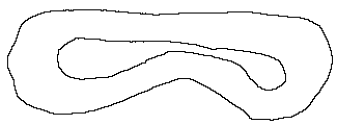
\includegraphics[interpolate=true,width=3.370000in,height=1.250000in]{contents/chapt6/figs/steer/lfc_paths-img0.png}}%
\end{pgfscope}%
\begin{pgfscope}%
\pgfpathrectangle{\pgfqpoint{1.188281in}{2.512600in}}{\pgfqpoint{3.364627in}{1.242324in}}%
\pgfusepath{clip}%
\pgfsetbuttcap%
\pgfsetroundjoin%
\pgfsetlinewidth{1.505625pt}%
\definecolor{currentstroke}{rgb}{0.501961,0.501961,0.501961}%
\pgfsetstrokecolor{currentstroke}%
\pgfsetdash{{5.550000pt}{2.400000pt}}{0.000000pt}%
\pgfpathmoveto{\pgfqpoint{3.050862in}{3.106006in}}%
\pgfpathlineto{\pgfqpoint{3.151999in}{3.083823in}}%
\pgfpathlineto{\pgfqpoint{3.212206in}{3.068515in}}%
\pgfpathlineto{\pgfqpoint{3.271753in}{3.050448in}}%
\pgfpathlineto{\pgfqpoint{3.310921in}{3.036504in}}%
\pgfpathlineto{\pgfqpoint{3.349490in}{3.020992in}}%
\pgfpathlineto{\pgfqpoint{3.387304in}{3.003888in}}%
\pgfpathlineto{\pgfqpoint{3.424208in}{2.985171in}}%
\pgfpathlineto{\pgfqpoint{3.460051in}{2.964818in}}%
\pgfpathlineto{\pgfqpoint{3.494792in}{2.942798in}}%
\pgfpathlineto{\pgfqpoint{3.528498in}{2.919068in}}%
\pgfpathlineto{\pgfqpoint{3.561239in}{2.893584in}}%
\pgfpathlineto{\pgfqpoint{3.593086in}{2.866306in}}%
\pgfpathlineto{\pgfqpoint{3.639469in}{2.822283in}}%
\pgfpathlineto{\pgfqpoint{3.685996in}{2.778603in}}%
\pgfpathlineto{\pgfqpoint{3.718466in}{2.752904in}}%
\pgfpathlineto{\pgfqpoint{3.735447in}{2.741813in}}%
\pgfpathlineto{\pgfqpoint{3.753063in}{2.732219in}}%
\pgfpathlineto{\pgfqpoint{3.771419in}{2.724367in}}%
\pgfpathlineto{\pgfqpoint{3.790561in}{2.718409in}}%
\pgfpathlineto{\pgfqpoint{3.810387in}{2.714264in}}%
\pgfpathlineto{\pgfqpoint{3.830774in}{2.711812in}}%
\pgfpathlineto{\pgfqpoint{3.851597in}{2.710934in}}%
\pgfpathlineto{\pgfqpoint{3.872730in}{2.711509in}}%
\pgfpathlineto{\pgfqpoint{3.894049in}{2.713418in}}%
\pgfpathlineto{\pgfqpoint{3.936746in}{2.720758in}}%
\pgfpathlineto{\pgfqpoint{3.978689in}{2.731996in}}%
\pgfpathlineto{\pgfqpoint{4.019024in}{2.746433in}}%
\pgfpathlineto{\pgfqpoint{4.057299in}{2.764101in}}%
\pgfpathlineto{\pgfqpoint{4.093131in}{2.785158in}}%
\pgfpathlineto{\pgfqpoint{4.110012in}{2.797007in}}%
\pgfpathlineto{\pgfqpoint{4.126139in}{2.809762in}}%
\pgfpathlineto{\pgfqpoint{4.141464in}{2.823444in}}%
\pgfpathlineto{\pgfqpoint{4.155939in}{2.838069in}}%
\pgfpathlineto{\pgfqpoint{4.169529in}{2.853618in}}%
\pgfpathlineto{\pgfqpoint{4.182212in}{2.870022in}}%
\pgfpathlineto{\pgfqpoint{4.193964in}{2.887213in}}%
\pgfpathlineto{\pgfqpoint{4.204764in}{2.905121in}}%
\pgfpathlineto{\pgfqpoint{4.214590in}{2.923676in}}%
\pgfpathlineto{\pgfqpoint{4.223419in}{2.942811in}}%
\pgfpathlineto{\pgfqpoint{4.231229in}{2.962454in}}%
\pgfpathlineto{\pgfqpoint{4.237999in}{2.982538in}}%
\pgfpathlineto{\pgfqpoint{4.243705in}{3.002992in}}%
\pgfpathlineto{\pgfqpoint{4.248325in}{3.023748in}}%
\pgfpathlineto{\pgfqpoint{4.251825in}{3.044725in}}%
\pgfpathlineto{\pgfqpoint{4.254156in}{3.065837in}}%
\pgfpathlineto{\pgfqpoint{4.255270in}{3.086995in}}%
\pgfpathlineto{\pgfqpoint{4.255118in}{3.108109in}}%
\pgfpathlineto{\pgfqpoint{4.253652in}{3.129092in}}%
\pgfpathlineto{\pgfqpoint{4.250823in}{3.149855in}}%
\pgfpathlineto{\pgfqpoint{4.246583in}{3.170308in}}%
\pgfpathlineto{\pgfqpoint{4.240882in}{3.190365in}}%
\pgfpathlineto{\pgfqpoint{4.233673in}{3.209934in}}%
\pgfpathlineto{\pgfqpoint{4.224916in}{3.228930in}}%
\pgfpathlineto{\pgfqpoint{4.214664in}{3.247268in}}%
\pgfpathlineto{\pgfqpoint{4.203026in}{3.264866in}}%
\pgfpathlineto{\pgfqpoint{4.190111in}{3.281645in}}%
\pgfpathlineto{\pgfqpoint{4.176031in}{3.297523in}}%
\pgfpathlineto{\pgfqpoint{4.160893in}{3.312419in}}%
\pgfpathlineto{\pgfqpoint{4.144809in}{3.326252in}}%
\pgfpathlineto{\pgfqpoint{4.127887in}{3.338941in}}%
\pgfpathlineto{\pgfqpoint{4.110238in}{3.350406in}}%
\pgfpathlineto{\pgfqpoint{4.091970in}{3.360565in}}%
\pgfpathlineto{\pgfqpoint{4.073188in}{3.369367in}}%
\pgfpathlineto{\pgfqpoint{4.053961in}{3.376912in}}%
\pgfpathlineto{\pgfqpoint{4.014399in}{3.388843in}}%
\pgfpathlineto{\pgfqpoint{3.973748in}{3.397573in}}%
\pgfpathlineto{\pgfqpoint{3.911738in}{3.407324in}}%
\pgfpathlineto{\pgfqpoint{3.686000in}{3.439363in}}%
\pgfpathlineto{\pgfqpoint{3.624214in}{3.444354in}}%
\pgfpathlineto{\pgfqpoint{3.562130in}{3.447073in}}%
\pgfpathlineto{\pgfqpoint{3.479138in}{3.448054in}}%
\pgfpathlineto{\pgfqpoint{3.313386in}{3.448023in}}%
\pgfpathlineto{\pgfqpoint{3.251467in}{3.451103in}}%
\pgfpathlineto{\pgfqpoint{3.189691in}{3.456926in}}%
\pgfpathlineto{\pgfqpoint{2.963087in}{3.482224in}}%
\pgfpathlineto{\pgfqpoint{2.901097in}{3.486031in}}%
\pgfpathlineto{\pgfqpoint{2.839064in}{3.487479in}}%
\pgfpathlineto{\pgfqpoint{2.777004in}{3.486661in}}%
\pgfpathlineto{\pgfqpoint{2.528391in}{3.480271in}}%
\pgfpathlineto{\pgfqpoint{2.466348in}{3.482502in}}%
\pgfpathlineto{\pgfqpoint{2.404508in}{3.487775in}}%
\pgfpathlineto{\pgfqpoint{2.219191in}{3.507483in}}%
\pgfpathlineto{\pgfqpoint{2.157089in}{3.509602in}}%
\pgfpathlineto{\pgfqpoint{2.094910in}{3.509391in}}%
\pgfpathlineto{\pgfqpoint{2.012136in}{3.506922in}}%
\pgfpathlineto{\pgfqpoint{1.950248in}{3.503652in}}%
\pgfpathlineto{\pgfqpoint{1.888437in}{3.497884in}}%
\pgfpathlineto{\pgfqpoint{1.847224in}{3.491982in}}%
\pgfpathlineto{\pgfqpoint{1.806005in}{3.483959in}}%
\pgfpathlineto{\pgfqpoint{1.765209in}{3.473312in}}%
\pgfpathlineto{\pgfqpoint{1.725566in}{3.459471in}}%
\pgfpathlineto{\pgfqpoint{1.706406in}{3.451174in}}%
\pgfpathlineto{\pgfqpoint{1.687809in}{3.441864in}}%
\pgfpathlineto{\pgfqpoint{1.669867in}{3.431469in}}%
\pgfpathlineto{\pgfqpoint{1.652673in}{3.419919in}}%
\pgfpathlineto{\pgfqpoint{1.636318in}{3.407142in}}%
\pgfpathlineto{\pgfqpoint{1.620878in}{3.393130in}}%
\pgfpathlineto{\pgfqpoint{1.606406in}{3.377979in}}%
\pgfpathlineto{\pgfqpoint{1.592953in}{3.361796in}}%
\pgfpathlineto{\pgfqpoint{1.580568in}{3.344688in}}%
\pgfpathlineto{\pgfqpoint{1.569301in}{3.326762in}}%
\pgfpathlineto{\pgfqpoint{1.559202in}{3.308123in}}%
\pgfpathlineto{\pgfqpoint{1.550322in}{3.288880in}}%
\pgfpathlineto{\pgfqpoint{1.542710in}{3.269138in}}%
\pgfpathlineto{\pgfqpoint{1.536416in}{3.249005in}}%
\pgfpathlineto{\pgfqpoint{1.531489in}{3.228586in}}%
\pgfpathlineto{\pgfqpoint{1.527945in}{3.207967in}}%
\pgfpathlineto{\pgfqpoint{1.525753in}{3.187203in}}%
\pgfpathlineto{\pgfqpoint{1.524882in}{3.166351in}}%
\pgfpathlineto{\pgfqpoint{1.525300in}{3.145465in}}%
\pgfpathlineto{\pgfqpoint{1.526973in}{3.124600in}}%
\pgfpathlineto{\pgfqpoint{1.529869in}{3.103811in}}%
\pgfpathlineto{\pgfqpoint{1.533956in}{3.083153in}}%
\pgfpathlineto{\pgfqpoint{1.539202in}{3.062681in}}%
\pgfpathlineto{\pgfqpoint{1.545573in}{3.042450in}}%
\pgfpathlineto{\pgfqpoint{1.553039in}{3.022518in}}%
\pgfpathlineto{\pgfqpoint{1.561573in}{3.002970in}}%
\pgfpathlineto{\pgfqpoint{1.571155in}{2.983919in}}%
\pgfpathlineto{\pgfqpoint{1.581764in}{2.965475in}}%
\pgfpathlineto{\pgfqpoint{1.593380in}{2.947749in}}%
\pgfpathlineto{\pgfqpoint{1.605982in}{2.930851in}}%
\pgfpathlineto{\pgfqpoint{1.619550in}{2.914892in}}%
\pgfpathlineto{\pgfqpoint{1.634063in}{2.899983in}}%
\pgfpathlineto{\pgfqpoint{1.649501in}{2.886236in}}%
\pgfpathlineto{\pgfqpoint{1.665843in}{2.873761in}}%
\pgfpathlineto{\pgfqpoint{1.683061in}{2.862649in}}%
\pgfpathlineto{\pgfqpoint{1.701080in}{2.852857in}}%
\pgfpathlineto{\pgfqpoint{1.719807in}{2.844287in}}%
\pgfpathlineto{\pgfqpoint{1.739144in}{2.836839in}}%
\pgfpathlineto{\pgfqpoint{1.779272in}{2.824912in}}%
\pgfpathlineto{\pgfqpoint{1.820705in}{2.816285in}}%
\pgfpathlineto{\pgfqpoint{1.862681in}{2.810163in}}%
\pgfpathlineto{\pgfqpoint{1.904553in}{2.805891in}}%
\pgfpathlineto{\pgfqpoint{1.946187in}{2.803433in}}%
\pgfpathlineto{\pgfqpoint{1.987591in}{2.802926in}}%
\pgfpathlineto{\pgfqpoint{2.028774in}{2.804510in}}%
\pgfpathlineto{\pgfqpoint{2.069744in}{2.808323in}}%
\pgfpathlineto{\pgfqpoint{2.110511in}{2.814409in}}%
\pgfpathlineto{\pgfqpoint{2.151079in}{2.822450in}}%
\pgfpathlineto{\pgfqpoint{2.211571in}{2.837295in}}%
\pgfpathlineto{\pgfqpoint{2.291578in}{2.860170in}}%
\pgfpathlineto{\pgfqpoint{2.370741in}{2.885006in}}%
\pgfpathlineto{\pgfqpoint{2.429342in}{2.905383in}}%
\pgfpathlineto{\pgfqpoint{2.487103in}{2.927760in}}%
\pgfpathlineto{\pgfqpoint{2.544060in}{2.952175in}}%
\pgfpathlineto{\pgfqpoint{2.619283in}{2.987005in}}%
\pgfpathlineto{\pgfqpoint{2.751276in}{3.048974in}}%
\pgfpathlineto{\pgfqpoint{2.789731in}{3.064339in}}%
\pgfpathlineto{\pgfqpoint{2.828797in}{3.077384in}}%
\pgfpathlineto{\pgfqpoint{2.868618in}{3.087451in}}%
\pgfpathlineto{\pgfqpoint{2.909168in}{3.094608in}}%
\pgfpathlineto{\pgfqpoint{2.950281in}{3.099509in}}%
\pgfpathlineto{\pgfqpoint{3.012644in}{3.104098in}}%
\pgfpathlineto{\pgfqpoint{3.033532in}{3.105226in}}%
\pgfpathlineto{\pgfqpoint{3.033532in}{3.105226in}}%
\pgfusepath{stroke}%
\end{pgfscope}%
\begin{pgfscope}%
\pgfpathrectangle{\pgfqpoint{1.188281in}{2.512600in}}{\pgfqpoint{3.364627in}{1.242324in}}%
\pgfusepath{clip}%
\pgfsetrectcap%
\pgfsetroundjoin%
\pgfsetlinewidth{1.505625pt}%
\definecolor{currentstroke}{rgb}{0.121569,0.466667,0.705882}%
\pgfsetstrokecolor{currentstroke}%
\pgfsetstrokeopacity{0.800000}%
\pgfsetdash{}{0pt}%
\pgfpathmoveto{\pgfqpoint{3.258821in}{3.444343in}}%
\pgfpathlineto{\pgfqpoint{3.140103in}{3.445291in}}%
\pgfpathlineto{\pgfqpoint{3.055496in}{3.448203in}}%
\pgfpathlineto{\pgfqpoint{2.983364in}{3.453073in}}%
\pgfpathlineto{\pgfqpoint{2.921403in}{3.459725in}}%
\pgfpathlineto{\pgfqpoint{2.870088in}{3.467689in}}%
\pgfpathlineto{\pgfqpoint{2.798794in}{3.481948in}}%
\pgfpathlineto{\pgfqpoint{2.717207in}{3.497682in}}%
\pgfpathlineto{\pgfqpoint{2.665806in}{3.505066in}}%
\pgfpathlineto{\pgfqpoint{2.603773in}{3.511029in}}%
\pgfpathlineto{\pgfqpoint{2.448548in}{3.524308in}}%
\pgfpathlineto{\pgfqpoint{2.303954in}{3.539704in}}%
\pgfpathlineto{\pgfqpoint{2.241764in}{3.543696in}}%
\pgfpathlineto{\pgfqpoint{2.179466in}{3.545245in}}%
\pgfpathlineto{\pgfqpoint{2.117156in}{3.544292in}}%
\pgfpathlineto{\pgfqpoint{2.054928in}{3.540949in}}%
\pgfpathlineto{\pgfqpoint{2.003251in}{3.535835in}}%
\pgfpathlineto{\pgfqpoint{1.962165in}{3.529685in}}%
\pgfpathlineto{\pgfqpoint{1.921482in}{3.521284in}}%
\pgfpathlineto{\pgfqpoint{1.881439in}{3.510232in}}%
\pgfpathlineto{\pgfqpoint{1.851991in}{3.500055in}}%
\pgfpathlineto{\pgfqpoint{1.823230in}{3.488077in}}%
\pgfpathlineto{\pgfqpoint{1.795462in}{3.473955in}}%
\pgfpathlineto{\pgfqpoint{1.768959in}{3.457582in}}%
\pgfpathlineto{\pgfqpoint{1.744036in}{3.438896in}}%
\pgfpathlineto{\pgfqpoint{1.721108in}{3.417813in}}%
\pgfpathlineto{\pgfqpoint{1.707120in}{3.402458in}}%
\pgfpathlineto{\pgfqpoint{1.694302in}{3.386115in}}%
\pgfpathlineto{\pgfqpoint{1.682763in}{3.368845in}}%
\pgfpathlineto{\pgfqpoint{1.672519in}{3.350776in}}%
\pgfpathlineto{\pgfqpoint{1.663631in}{3.332003in}}%
\pgfpathlineto{\pgfqpoint{1.656160in}{3.312623in}}%
\pgfpathlineto{\pgfqpoint{1.650172in}{3.292735in}}%
\pgfpathlineto{\pgfqpoint{1.645714in}{3.272449in}}%
\pgfpathlineto{\pgfqpoint{1.642799in}{3.251885in}}%
\pgfpathlineto{\pgfqpoint{1.641438in}{3.231160in}}%
\pgfpathlineto{\pgfqpoint{1.641639in}{3.210391in}}%
\pgfpathlineto{\pgfqpoint{1.643402in}{3.189696in}}%
\pgfpathlineto{\pgfqpoint{1.646783in}{3.169203in}}%
\pgfpathlineto{\pgfqpoint{1.651698in}{3.149023in}}%
\pgfpathlineto{\pgfqpoint{1.658193in}{3.129294in}}%
\pgfpathlineto{\pgfqpoint{1.666233in}{3.110144in}}%
\pgfpathlineto{\pgfqpoint{1.675805in}{3.091712in}}%
\pgfpathlineto{\pgfqpoint{1.686854in}{3.074125in}}%
\pgfpathlineto{\pgfqpoint{1.699323in}{3.057516in}}%
\pgfpathlineto{\pgfqpoint{1.713164in}{3.042030in}}%
\pgfpathlineto{\pgfqpoint{1.728286in}{3.027794in}}%
\pgfpathlineto{\pgfqpoint{1.744590in}{3.014929in}}%
\pgfpathlineto{\pgfqpoint{1.761945in}{3.003521in}}%
\pgfpathlineto{\pgfqpoint{1.780172in}{2.993562in}}%
\pgfpathlineto{\pgfqpoint{1.799103in}{2.985017in}}%
\pgfpathlineto{\pgfqpoint{1.828486in}{2.974675in}}%
\pgfpathlineto{\pgfqpoint{1.858651in}{2.966886in}}%
\pgfpathlineto{\pgfqpoint{1.899512in}{2.959407in}}%
\pgfpathlineto{\pgfqpoint{1.951064in}{2.953157in}}%
\pgfpathlineto{\pgfqpoint{2.002839in}{2.949134in}}%
\pgfpathlineto{\pgfqpoint{2.054738in}{2.947360in}}%
\pgfpathlineto{\pgfqpoint{2.096280in}{2.947858in}}%
\pgfpathlineto{\pgfqpoint{2.137745in}{2.950407in}}%
\pgfpathlineto{\pgfqpoint{2.179028in}{2.955056in}}%
\pgfpathlineto{\pgfqpoint{2.250887in}{2.966123in}}%
\pgfpathlineto{\pgfqpoint{2.333031in}{2.978631in}}%
\pgfpathlineto{\pgfqpoint{2.384663in}{2.984198in}}%
\pgfpathlineto{\pgfqpoint{2.508754in}{2.995674in}}%
\pgfpathlineto{\pgfqpoint{2.539446in}{3.001033in}}%
\pgfpathlineto{\pgfqpoint{2.569734in}{3.008336in}}%
\pgfpathlineto{\pgfqpoint{2.599413in}{3.017808in}}%
\pgfpathlineto{\pgfqpoint{2.628361in}{3.029328in}}%
\pgfpathlineto{\pgfqpoint{2.665801in}{3.047323in}}%
\pgfpathlineto{\pgfqpoint{2.711278in}{3.072396in}}%
\pgfpathlineto{\pgfqpoint{2.819031in}{3.134030in}}%
\pgfpathlineto{\pgfqpoint{2.846850in}{3.147129in}}%
\pgfpathlineto{\pgfqpoint{2.875434in}{3.158116in}}%
\pgfpathlineto{\pgfqpoint{2.904746in}{3.166540in}}%
\pgfpathlineto{\pgfqpoint{2.934643in}{3.171892in}}%
\pgfpathlineto{\pgfqpoint{2.954930in}{3.173592in}}%
\pgfpathlineto{\pgfqpoint{2.985789in}{3.173409in}}%
\pgfpathlineto{\pgfqpoint{3.016757in}{3.170278in}}%
\pgfpathlineto{\pgfqpoint{3.047353in}{3.164554in}}%
\pgfpathlineto{\pgfqpoint{3.077404in}{3.156437in}}%
\pgfpathlineto{\pgfqpoint{3.106752in}{3.146062in}}%
\pgfpathlineto{\pgfqpoint{3.135282in}{3.133610in}}%
\pgfpathlineto{\pgfqpoint{3.162849in}{3.119149in}}%
\pgfpathlineto{\pgfqpoint{3.198183in}{3.097374in}}%
\pgfpathlineto{\pgfqpoint{3.240657in}{3.067572in}}%
\pgfpathlineto{\pgfqpoint{3.308270in}{3.019398in}}%
\pgfpathlineto{\pgfqpoint{3.343342in}{2.997195in}}%
\pgfpathlineto{\pgfqpoint{3.379435in}{2.976693in}}%
\pgfpathlineto{\pgfqpoint{3.443931in}{2.943262in}}%
\pgfpathlineto{\pgfqpoint{3.517388in}{2.904575in}}%
\pgfpathlineto{\pgfqpoint{3.699432in}{2.804903in}}%
\pgfpathlineto{\pgfqpoint{3.737008in}{2.787268in}}%
\pgfpathlineto{\pgfqpoint{3.765879in}{2.775623in}}%
\pgfpathlineto{\pgfqpoint{3.795481in}{2.766000in}}%
\pgfpathlineto{\pgfqpoint{3.825832in}{2.759108in}}%
\pgfpathlineto{\pgfqpoint{3.846394in}{2.756306in}}%
\pgfpathlineto{\pgfqpoint{3.867113in}{2.755125in}}%
\pgfpathlineto{\pgfqpoint{3.887857in}{2.755696in}}%
\pgfpathlineto{\pgfqpoint{3.908477in}{2.758025in}}%
\pgfpathlineto{\pgfqpoint{3.928830in}{2.762074in}}%
\pgfpathlineto{\pgfqpoint{3.948751in}{2.767884in}}%
\pgfpathlineto{\pgfqpoint{3.968073in}{2.775453in}}%
\pgfpathlineto{\pgfqpoint{3.986643in}{2.784714in}}%
\pgfpathlineto{\pgfqpoint{4.004321in}{2.795581in}}%
\pgfpathlineto{\pgfqpoint{4.020977in}{2.807957in}}%
\pgfpathlineto{\pgfqpoint{4.036494in}{2.821736in}}%
\pgfpathlineto{\pgfqpoint{4.050716in}{2.836847in}}%
\pgfpathlineto{\pgfqpoint{4.063541in}{2.853161in}}%
\pgfpathlineto{\pgfqpoint{4.074921in}{2.870514in}}%
\pgfpathlineto{\pgfqpoint{4.084707in}{2.888813in}}%
\pgfpathlineto{\pgfqpoint{4.092882in}{2.907886in}}%
\pgfpathlineto{\pgfqpoint{4.099319in}{2.927614in}}%
\pgfpathlineto{\pgfqpoint{4.103969in}{2.947838in}}%
\pgfpathlineto{\pgfqpoint{4.106792in}{2.968396in}}%
\pgfpathlineto{\pgfqpoint{4.107757in}{2.989125in}}%
\pgfpathlineto{\pgfqpoint{4.106850in}{3.009857in}}%
\pgfpathlineto{\pgfqpoint{4.104037in}{3.030416in}}%
\pgfpathlineto{\pgfqpoint{4.099341in}{3.050629in}}%
\pgfpathlineto{\pgfqpoint{4.092911in}{3.070359in}}%
\pgfpathlineto{\pgfqpoint{4.084897in}{3.089502in}}%
\pgfpathlineto{\pgfqpoint{4.075434in}{3.107971in}}%
\pgfpathlineto{\pgfqpoint{4.064551in}{3.125641in}}%
\pgfpathlineto{\pgfqpoint{4.052369in}{3.142442in}}%
\pgfpathlineto{\pgfqpoint{4.031907in}{3.165892in}}%
\pgfpathlineto{\pgfqpoint{4.009063in}{3.187028in}}%
\pgfpathlineto{\pgfqpoint{3.984164in}{3.205699in}}%
\pgfpathlineto{\pgfqpoint{3.957606in}{3.221932in}}%
\pgfpathlineto{\pgfqpoint{3.929824in}{3.235974in}}%
\pgfpathlineto{\pgfqpoint{3.891529in}{3.251978in}}%
\pgfpathlineto{\pgfqpoint{3.832907in}{3.272968in}}%
\pgfpathlineto{\pgfqpoint{3.745034in}{3.304622in}}%
\pgfpathlineto{\pgfqpoint{3.667082in}{3.333187in}}%
\pgfpathlineto{\pgfqpoint{3.627484in}{3.345637in}}%
\pgfpathlineto{\pgfqpoint{3.587270in}{3.355915in}}%
\pgfpathlineto{\pgfqpoint{3.546514in}{3.363782in}}%
\pgfpathlineto{\pgfqpoint{3.505419in}{3.369629in}}%
\pgfpathlineto{\pgfqpoint{3.464104in}{3.373641in}}%
\pgfpathlineto{\pgfqpoint{3.412292in}{3.376437in}}%
\pgfpathlineto{\pgfqpoint{3.350033in}{3.377453in}}%
\pgfpathlineto{\pgfqpoint{3.256631in}{3.377994in}}%
\pgfpathlineto{\pgfqpoint{3.256631in}{3.377994in}}%
\pgfusepath{stroke}%
\end{pgfscope}%
\begin{pgfscope}%
\pgfpathrectangle{\pgfqpoint{1.188281in}{2.512600in}}{\pgfqpoint{3.364627in}{1.242324in}}%
\pgfusepath{clip}%
\pgfsetrectcap%
\pgfsetroundjoin%
\pgfsetlinewidth{1.505625pt}%
\definecolor{currentstroke}{rgb}{1.000000,0.498039,0.054902}%
\pgfsetstrokecolor{currentstroke}%
\pgfsetstrokeopacity{0.800000}%
\pgfsetdash{}{0pt}%
\pgfpathmoveto{\pgfqpoint{3.258821in}{3.444343in}}%
\pgfpathlineto{\pgfqpoint{3.197933in}{3.443492in}}%
\pgfpathlineto{\pgfqpoint{3.142903in}{3.440199in}}%
\pgfpathlineto{\pgfqpoint{3.090605in}{3.434737in}}%
\pgfpathlineto{\pgfqpoint{2.949122in}{3.416703in}}%
\pgfpathlineto{\pgfqpoint{2.908917in}{3.414782in}}%
\pgfpathlineto{\pgfqpoint{2.867938in}{3.415202in}}%
\pgfpathlineto{\pgfqpoint{2.826531in}{3.417624in}}%
\pgfpathlineto{\pgfqpoint{2.774938in}{3.423187in}}%
\pgfpathlineto{\pgfqpoint{2.723707in}{3.431447in}}%
\pgfpathlineto{\pgfqpoint{2.672918in}{3.442100in}}%
\pgfpathlineto{\pgfqpoint{2.480569in}{3.485517in}}%
\pgfpathlineto{\pgfqpoint{2.419162in}{3.495883in}}%
\pgfpathlineto{\pgfqpoint{2.357455in}{3.504267in}}%
\pgfpathlineto{\pgfqpoint{2.295504in}{3.510608in}}%
\pgfpathlineto{\pgfqpoint{2.233370in}{3.514782in}}%
\pgfpathlineto{\pgfqpoint{2.181495in}{3.516201in}}%
\pgfpathlineto{\pgfqpoint{2.129606in}{3.515484in}}%
\pgfpathlineto{\pgfqpoint{2.077802in}{3.512438in}}%
\pgfpathlineto{\pgfqpoint{2.036526in}{3.508007in}}%
\pgfpathlineto{\pgfqpoint{2.005799in}{3.502979in}}%
\pgfpathlineto{\pgfqpoint{1.975400in}{3.496251in}}%
\pgfpathlineto{\pgfqpoint{1.945488in}{3.487618in}}%
\pgfpathlineto{\pgfqpoint{1.916298in}{3.476796in}}%
\pgfpathlineto{\pgfqpoint{1.888071in}{3.463665in}}%
\pgfpathlineto{\pgfqpoint{1.861015in}{3.448266in}}%
\pgfpathlineto{\pgfqpoint{1.835218in}{3.430837in}}%
\pgfpathlineto{\pgfqpoint{1.810791in}{3.411537in}}%
\pgfpathlineto{\pgfqpoint{1.787818in}{3.390524in}}%
\pgfpathlineto{\pgfqpoint{1.766313in}{3.368011in}}%
\pgfpathlineto{\pgfqpoint{1.746341in}{3.344127in}}%
\pgfpathlineto{\pgfqpoint{1.727975in}{3.318988in}}%
\pgfpathlineto{\pgfqpoint{1.711435in}{3.292613in}}%
\pgfpathlineto{\pgfqpoint{1.697182in}{3.264938in}}%
\pgfpathlineto{\pgfqpoint{1.685598in}{3.236046in}}%
\pgfpathlineto{\pgfqpoint{1.677040in}{3.206121in}}%
\pgfpathlineto{\pgfqpoint{1.673193in}{3.185725in}}%
\pgfpathlineto{\pgfqpoint{1.670918in}{3.165095in}}%
\pgfpathlineto{\pgfqpoint{1.670266in}{3.144350in}}%
\pgfpathlineto{\pgfqpoint{1.671291in}{3.123620in}}%
\pgfpathlineto{\pgfqpoint{1.673919in}{3.103032in}}%
\pgfpathlineto{\pgfqpoint{1.678130in}{3.082708in}}%
\pgfpathlineto{\pgfqpoint{1.683898in}{3.062770in}}%
\pgfpathlineto{\pgfqpoint{1.691170in}{3.043330in}}%
\pgfpathlineto{\pgfqpoint{1.699911in}{3.024505in}}%
\pgfpathlineto{\pgfqpoint{1.710070in}{3.006406in}}%
\pgfpathlineto{\pgfqpoint{1.721570in}{2.989128in}}%
\pgfpathlineto{\pgfqpoint{1.734338in}{2.972765in}}%
\pgfpathlineto{\pgfqpoint{1.748300in}{2.957407in}}%
\pgfpathlineto{\pgfqpoint{1.763376in}{2.943143in}}%
\pgfpathlineto{\pgfqpoint{1.787835in}{2.923892in}}%
\pgfpathlineto{\pgfqpoint{1.814053in}{2.907109in}}%
\pgfpathlineto{\pgfqpoint{1.841610in}{2.892626in}}%
\pgfpathlineto{\pgfqpoint{1.870252in}{2.880428in}}%
\pgfpathlineto{\pgfqpoint{1.899730in}{2.870412in}}%
\pgfpathlineto{\pgfqpoint{1.929817in}{2.862405in}}%
\pgfpathlineto{\pgfqpoint{1.960343in}{2.856280in}}%
\pgfpathlineto{\pgfqpoint{2.001433in}{2.850363in}}%
\pgfpathlineto{\pgfqpoint{2.042766in}{2.846477in}}%
\pgfpathlineto{\pgfqpoint{2.094591in}{2.843805in}}%
\pgfpathlineto{\pgfqpoint{2.156861in}{2.843130in}}%
\pgfpathlineto{\pgfqpoint{2.208736in}{2.844582in}}%
\pgfpathlineto{\pgfqpoint{2.260517in}{2.848011in}}%
\pgfpathlineto{\pgfqpoint{2.312104in}{2.853647in}}%
\pgfpathlineto{\pgfqpoint{2.363378in}{2.861641in}}%
\pgfpathlineto{\pgfqpoint{2.414264in}{2.871820in}}%
\pgfpathlineto{\pgfqpoint{2.464702in}{2.884029in}}%
\pgfpathlineto{\pgfqpoint{2.524598in}{2.901070in}}%
\pgfpathlineto{\pgfqpoint{2.583782in}{2.920445in}}%
\pgfpathlineto{\pgfqpoint{2.671617in}{2.952244in}}%
\pgfpathlineto{\pgfqpoint{2.866238in}{3.024384in}}%
\pgfpathlineto{\pgfqpoint{2.906091in}{3.036012in}}%
\pgfpathlineto{\pgfqpoint{2.946479in}{3.045614in}}%
\pgfpathlineto{\pgfqpoint{2.987364in}{3.052788in}}%
\pgfpathlineto{\pgfqpoint{3.018335in}{3.055963in}}%
\pgfpathlineto{\pgfqpoint{3.049452in}{3.056973in}}%
\pgfpathlineto{\pgfqpoint{3.080551in}{3.055587in}}%
\pgfpathlineto{\pgfqpoint{3.111419in}{3.051555in}}%
\pgfpathlineto{\pgfqpoint{3.141803in}{3.044786in}}%
\pgfpathlineto{\pgfqpoint{3.171421in}{3.035204in}}%
\pgfpathlineto{\pgfqpoint{3.200107in}{3.023111in}}%
\pgfpathlineto{\pgfqpoint{3.227827in}{3.008935in}}%
\pgfpathlineto{\pgfqpoint{3.263460in}{2.987641in}}%
\pgfpathlineto{\pgfqpoint{3.297836in}{2.964365in}}%
\pgfpathlineto{\pgfqpoint{3.347936in}{2.927376in}}%
\pgfpathlineto{\pgfqpoint{3.406429in}{2.884285in}}%
\pgfpathlineto{\pgfqpoint{3.440965in}{2.861248in}}%
\pgfpathlineto{\pgfqpoint{3.476700in}{2.840122in}}%
\pgfpathlineto{\pgfqpoint{3.504378in}{2.825862in}}%
\pgfpathlineto{\pgfqpoint{3.542412in}{2.809233in}}%
\pgfpathlineto{\pgfqpoint{3.581368in}{2.794884in}}%
\pgfpathlineto{\pgfqpoint{3.630792in}{2.779064in}}%
\pgfpathlineto{\pgfqpoint{3.720632in}{2.753470in}}%
\pgfpathlineto{\pgfqpoint{3.780980in}{2.738108in}}%
\pgfpathlineto{\pgfqpoint{3.821746in}{2.730284in}}%
\pgfpathlineto{\pgfqpoint{3.852673in}{2.726713in}}%
\pgfpathlineto{\pgfqpoint{3.883784in}{2.725644in}}%
\pgfpathlineto{\pgfqpoint{3.914851in}{2.727572in}}%
\pgfpathlineto{\pgfqpoint{3.935374in}{2.730672in}}%
\pgfpathlineto{\pgfqpoint{3.955610in}{2.735287in}}%
\pgfpathlineto{\pgfqpoint{3.975445in}{2.741400in}}%
\pgfpathlineto{\pgfqpoint{3.994726in}{2.749081in}}%
\pgfpathlineto{\pgfqpoint{4.013321in}{2.758300in}}%
\pgfpathlineto{\pgfqpoint{4.031100in}{2.769010in}}%
\pgfpathlineto{\pgfqpoint{4.047935in}{2.781148in}}%
\pgfpathlineto{\pgfqpoint{4.063707in}{2.794639in}}%
\pgfpathlineto{\pgfqpoint{4.078303in}{2.809394in}}%
\pgfpathlineto{\pgfqpoint{4.091616in}{2.825317in}}%
\pgfpathlineto{\pgfqpoint{4.103552in}{2.842296in}}%
\pgfpathlineto{\pgfqpoint{4.114079in}{2.860183in}}%
\pgfpathlineto{\pgfqpoint{4.123067in}{2.878890in}}%
\pgfpathlineto{\pgfqpoint{4.130462in}{2.898283in}}%
\pgfpathlineto{\pgfqpoint{4.136215in}{2.918225in}}%
\pgfpathlineto{\pgfqpoint{4.140288in}{2.938576in}}%
\pgfpathlineto{\pgfqpoint{4.142649in}{2.959196in}}%
\pgfpathlineto{\pgfqpoint{4.143282in}{2.979941in}}%
\pgfpathlineto{\pgfqpoint{4.142179in}{3.000667in}}%
\pgfpathlineto{\pgfqpoint{4.139346in}{3.021227in}}%
\pgfpathlineto{\pgfqpoint{4.134863in}{3.041492in}}%
\pgfpathlineto{\pgfqpoint{4.128755in}{3.061328in}}%
\pgfpathlineto{\pgfqpoint{4.121069in}{3.080607in}}%
\pgfpathlineto{\pgfqpoint{4.111867in}{3.099210in}}%
\pgfpathlineto{\pgfqpoint{4.101218in}{3.117025in}}%
\pgfpathlineto{\pgfqpoint{4.089201in}{3.133948in}}%
\pgfpathlineto{\pgfqpoint{4.075900in}{3.149880in}}%
\pgfpathlineto{\pgfqpoint{4.061401in}{3.164731in}}%
\pgfpathlineto{\pgfqpoint{4.045799in}{3.178418in}}%
\pgfpathlineto{\pgfqpoint{4.029189in}{3.190864in}}%
\pgfpathlineto{\pgfqpoint{4.002659in}{3.207142in}}%
\pgfpathlineto{\pgfqpoint{3.974647in}{3.220720in}}%
\pgfpathlineto{\pgfqpoint{3.945598in}{3.231917in}}%
\pgfpathlineto{\pgfqpoint{3.905899in}{3.244049in}}%
\pgfpathlineto{\pgfqpoint{3.835482in}{3.261944in}}%
\pgfpathlineto{\pgfqpoint{3.735030in}{3.288060in}}%
\pgfpathlineto{\pgfqpoint{3.665377in}{3.308728in}}%
\pgfpathlineto{\pgfqpoint{3.486829in}{3.363694in}}%
\pgfpathlineto{\pgfqpoint{3.426463in}{3.378990in}}%
\pgfpathlineto{\pgfqpoint{3.365626in}{3.392298in}}%
\pgfpathlineto{\pgfqpoint{3.304417in}{3.403768in}}%
\pgfpathlineto{\pgfqpoint{3.253158in}{3.411880in}}%
\pgfpathlineto{\pgfqpoint{3.253158in}{3.411880in}}%
\pgfusepath{stroke}%
\end{pgfscope}%
\begin{pgfscope}%
\pgfpathrectangle{\pgfqpoint{1.188281in}{2.512600in}}{\pgfqpoint{3.364627in}{1.242324in}}%
\pgfusepath{clip}%
\pgfsetrectcap%
\pgfsetroundjoin%
\pgfsetlinewidth{1.505625pt}%
\definecolor{currentstroke}{rgb}{0.172549,0.627451,0.172549}%
\pgfsetstrokecolor{currentstroke}%
\pgfsetstrokeopacity{0.800000}%
\pgfsetdash{}{0pt}%
\pgfpathmoveto{\pgfqpoint{3.258821in}{3.444343in}}%
\pgfpathlineto{\pgfqpoint{3.200200in}{3.445442in}}%
\pgfpathlineto{\pgfqpoint{3.165091in}{3.448404in}}%
\pgfpathlineto{\pgfqpoint{3.128334in}{3.453678in}}%
\pgfpathlineto{\pgfqpoint{3.089995in}{3.461647in}}%
\pgfpathlineto{\pgfqpoint{3.041426in}{3.474234in}}%
\pgfpathlineto{\pgfqpoint{2.981099in}{3.492225in}}%
\pgfpathlineto{\pgfqpoint{2.907258in}{3.516836in}}%
\pgfpathlineto{\pgfqpoint{2.838397in}{3.539394in}}%
\pgfpathlineto{\pgfqpoint{2.798334in}{3.550534in}}%
\pgfpathlineto{\pgfqpoint{2.757747in}{3.559570in}}%
\pgfpathlineto{\pgfqpoint{2.716660in}{3.565951in}}%
\pgfpathlineto{\pgfqpoint{2.675262in}{3.569856in}}%
\pgfpathlineto{\pgfqpoint{2.623336in}{3.572190in}}%
\pgfpathlineto{\pgfqpoint{2.560959in}{3.572446in}}%
\pgfpathlineto{\pgfqpoint{2.436209in}{3.572079in}}%
\pgfpathlineto{\pgfqpoint{2.384285in}{3.574487in}}%
\pgfpathlineto{\pgfqpoint{2.332520in}{3.579196in}}%
\pgfpathlineto{\pgfqpoint{2.281023in}{3.586265in}}%
\pgfpathlineto{\pgfqpoint{2.188409in}{3.599557in}}%
\pgfpathlineto{\pgfqpoint{2.146984in}{3.603159in}}%
\pgfpathlineto{\pgfqpoint{2.115812in}{3.604133in}}%
\pgfpathlineto{\pgfqpoint{2.084642in}{3.603179in}}%
\pgfpathlineto{\pgfqpoint{2.053614in}{3.600067in}}%
\pgfpathlineto{\pgfqpoint{2.022906in}{3.594643in}}%
\pgfpathlineto{\pgfqpoint{1.992700in}{3.586895in}}%
\pgfpathlineto{\pgfqpoint{1.963196in}{3.576805in}}%
\pgfpathlineto{\pgfqpoint{1.934590in}{3.564391in}}%
\pgfpathlineto{\pgfqpoint{1.907060in}{3.549747in}}%
\pgfpathlineto{\pgfqpoint{1.880714in}{3.533066in}}%
\pgfpathlineto{\pgfqpoint{1.855686in}{3.514463in}}%
\pgfpathlineto{\pgfqpoint{1.832073in}{3.494095in}}%
\pgfpathlineto{\pgfqpoint{1.809973in}{3.472094in}}%
\pgfpathlineto{\pgfqpoint{1.789450in}{3.448615in}}%
\pgfpathlineto{\pgfqpoint{1.770590in}{3.423780in}}%
\pgfpathlineto{\pgfqpoint{1.753473in}{3.397714in}}%
\pgfpathlineto{\pgfqpoint{1.738258in}{3.370493in}}%
\pgfpathlineto{\pgfqpoint{1.724929in}{3.342301in}}%
\pgfpathlineto{\pgfqpoint{1.713567in}{3.313260in}}%
\pgfpathlineto{\pgfqpoint{1.704208in}{3.283513in}}%
\pgfpathlineto{\pgfqpoint{1.696903in}{3.253196in}}%
\pgfpathlineto{\pgfqpoint{1.691652in}{3.222456in}}%
\pgfpathlineto{\pgfqpoint{1.688583in}{3.191424in}}%
\pgfpathlineto{\pgfqpoint{1.687991in}{3.160248in}}%
\pgfpathlineto{\pgfqpoint{1.689942in}{3.129127in}}%
\pgfpathlineto{\pgfqpoint{1.694569in}{3.098291in}}%
\pgfpathlineto{\pgfqpoint{1.701953in}{3.067998in}}%
\pgfpathlineto{\pgfqpoint{1.712157in}{3.038536in}}%
\pgfpathlineto{\pgfqpoint{1.725153in}{3.010194in}}%
\pgfpathlineto{\pgfqpoint{1.740778in}{2.983212in}}%
\pgfpathlineto{\pgfqpoint{1.758908in}{2.957846in}}%
\pgfpathlineto{\pgfqpoint{1.779354in}{2.934306in}}%
\pgfpathlineto{\pgfqpoint{1.801858in}{2.912723in}}%
\pgfpathlineto{\pgfqpoint{1.826173in}{2.893203in}}%
\pgfpathlineto{\pgfqpoint{1.852086in}{2.875859in}}%
\pgfpathlineto{\pgfqpoint{1.879331in}{2.860692in}}%
\pgfpathlineto{\pgfqpoint{1.907671in}{2.847682in}}%
\pgfpathlineto{\pgfqpoint{1.936904in}{2.836824in}}%
\pgfpathlineto{\pgfqpoint{1.966815in}{2.828001in}}%
\pgfpathlineto{\pgfqpoint{1.997240in}{2.821157in}}%
\pgfpathlineto{\pgfqpoint{2.028036in}{2.816246in}}%
\pgfpathlineto{\pgfqpoint{2.059072in}{2.813187in}}%
\pgfpathlineto{\pgfqpoint{2.090235in}{2.812012in}}%
\pgfpathlineto{\pgfqpoint{2.121412in}{2.812758in}}%
\pgfpathlineto{\pgfqpoint{2.152485in}{2.815404in}}%
\pgfpathlineto{\pgfqpoint{2.183331in}{2.819988in}}%
\pgfpathlineto{\pgfqpoint{2.213828in}{2.826504in}}%
\pgfpathlineto{\pgfqpoint{2.243847in}{2.834955in}}%
\pgfpathlineto{\pgfqpoint{2.273299in}{2.845207in}}%
\pgfpathlineto{\pgfqpoint{2.311670in}{2.861229in}}%
\pgfpathlineto{\pgfqpoint{2.358613in}{2.883550in}}%
\pgfpathlineto{\pgfqpoint{2.507734in}{2.957234in}}%
\pgfpathlineto{\pgfqpoint{2.555471in}{2.977803in}}%
\pgfpathlineto{\pgfqpoint{2.603894in}{2.996704in}}%
\pgfpathlineto{\pgfqpoint{2.662846in}{3.017084in}}%
\pgfpathlineto{\pgfqpoint{2.712736in}{3.031669in}}%
\pgfpathlineto{\pgfqpoint{2.753138in}{3.041511in}}%
\pgfpathlineto{\pgfqpoint{2.793945in}{3.049504in}}%
\pgfpathlineto{\pgfqpoint{2.835098in}{3.055464in}}%
\pgfpathlineto{\pgfqpoint{2.876511in}{3.059198in}}%
\pgfpathlineto{\pgfqpoint{2.918073in}{3.060434in}}%
\pgfpathlineto{\pgfqpoint{2.959630in}{3.059047in}}%
\pgfpathlineto{\pgfqpoint{3.001003in}{3.054912in}}%
\pgfpathlineto{\pgfqpoint{3.041995in}{3.047948in}}%
\pgfpathlineto{\pgfqpoint{3.082421in}{3.038219in}}%
\pgfpathlineto{\pgfqpoint{3.122250in}{3.026274in}}%
\pgfpathlineto{\pgfqpoint{3.161441in}{3.012374in}}%
\pgfpathlineto{\pgfqpoint{3.209573in}{2.992750in}}%
\pgfpathlineto{\pgfqpoint{3.256828in}{2.971095in}}%
\pgfpathlineto{\pgfqpoint{3.303143in}{2.947499in}}%
\pgfpathlineto{\pgfqpoint{3.348425in}{2.921977in}}%
\pgfpathlineto{\pgfqpoint{3.392536in}{2.894479in}}%
\pgfpathlineto{\pgfqpoint{3.435507in}{2.865232in}}%
\pgfpathlineto{\pgfqpoint{3.546493in}{2.788116in}}%
\pgfpathlineto{\pgfqpoint{3.590739in}{2.760840in}}%
\pgfpathlineto{\pgfqpoint{3.627214in}{2.740874in}}%
\pgfpathlineto{\pgfqpoint{3.655405in}{2.727539in}}%
\pgfpathlineto{\pgfqpoint{3.684335in}{2.715894in}}%
\pgfpathlineto{\pgfqpoint{3.713960in}{2.706156in}}%
\pgfpathlineto{\pgfqpoint{3.744211in}{2.698586in}}%
\pgfpathlineto{\pgfqpoint{3.774955in}{2.693379in}}%
\pgfpathlineto{\pgfqpoint{3.805861in}{2.690725in}}%
\pgfpathlineto{\pgfqpoint{3.836389in}{2.690876in}}%
\pgfpathlineto{\pgfqpoint{3.866269in}{2.693965in}}%
\pgfpathlineto{\pgfqpoint{3.895176in}{2.700099in}}%
\pgfpathlineto{\pgfqpoint{3.922767in}{2.709221in}}%
\pgfpathlineto{\pgfqpoint{3.940250in}{2.716930in}}%
\pgfpathlineto{\pgfqpoint{3.956883in}{2.725887in}}%
\pgfpathlineto{\pgfqpoint{3.972568in}{2.736020in}}%
\pgfpathlineto{\pgfqpoint{3.987599in}{2.747582in}}%
\pgfpathlineto{\pgfqpoint{4.009117in}{2.767472in}}%
\pgfpathlineto{\pgfqpoint{4.029500in}{2.789945in}}%
\pgfpathlineto{\pgfqpoint{4.048829in}{2.814514in}}%
\pgfpathlineto{\pgfqpoint{4.066607in}{2.840367in}}%
\pgfpathlineto{\pgfqpoint{4.082709in}{2.867295in}}%
\pgfpathlineto{\pgfqpoint{4.096928in}{2.895262in}}%
\pgfpathlineto{\pgfqpoint{4.109055in}{2.924198in}}%
\pgfpathlineto{\pgfqpoint{4.118858in}{2.953999in}}%
\pgfpathlineto{\pgfqpoint{4.126177in}{2.984505in}}%
\pgfpathlineto{\pgfqpoint{4.130859in}{3.015526in}}%
\pgfpathlineto{\pgfqpoint{4.132829in}{3.046835in}}%
\pgfpathlineto{\pgfqpoint{4.132014in}{3.078195in}}%
\pgfpathlineto{\pgfqpoint{4.128413in}{3.109359in}}%
\pgfpathlineto{\pgfqpoint{4.122022in}{3.140072in}}%
\pgfpathlineto{\pgfqpoint{4.112899in}{3.170087in}}%
\pgfpathlineto{\pgfqpoint{4.101098in}{3.199153in}}%
\pgfpathlineto{\pgfqpoint{4.086726in}{3.227038in}}%
\pgfpathlineto{\pgfqpoint{4.069884in}{3.253504in}}%
\pgfpathlineto{\pgfqpoint{4.050649in}{3.278285in}}%
\pgfpathlineto{\pgfqpoint{4.029163in}{3.301143in}}%
\pgfpathlineto{\pgfqpoint{4.005665in}{3.321926in}}%
\pgfpathlineto{\pgfqpoint{3.980346in}{3.340447in}}%
\pgfpathlineto{\pgfqpoint{3.953415in}{3.356535in}}%
\pgfpathlineto{\pgfqpoint{3.925119in}{3.370077in}}%
\pgfpathlineto{\pgfqpoint{3.895695in}{3.380957in}}%
\pgfpathlineto{\pgfqpoint{3.865403in}{3.389110in}}%
\pgfpathlineto{\pgfqpoint{3.834496in}{3.394494in}}%
\pgfpathlineto{\pgfqpoint{3.803257in}{3.397399in}}%
\pgfpathlineto{\pgfqpoint{3.771893in}{3.398258in}}%
\pgfpathlineto{\pgfqpoint{3.730069in}{3.397213in}}%
\pgfpathlineto{\pgfqpoint{3.646446in}{3.394332in}}%
\pgfpathlineto{\pgfqpoint{3.604628in}{3.395481in}}%
\pgfpathlineto{\pgfqpoint{3.573381in}{3.398319in}}%
\pgfpathlineto{\pgfqpoint{3.542384in}{3.403173in}}%
\pgfpathlineto{\pgfqpoint{3.511809in}{3.410213in}}%
\pgfpathlineto{\pgfqpoint{3.481818in}{3.419426in}}%
\pgfpathlineto{\pgfqpoint{3.452560in}{3.430752in}}%
\pgfpathlineto{\pgfqpoint{3.424176in}{3.444122in}}%
\pgfpathlineto{\pgfqpoint{3.387619in}{3.464459in}}%
\pgfpathlineto{\pgfqpoint{3.343350in}{3.492303in}}%
\pgfpathlineto{\pgfqpoint{3.290179in}{3.525635in}}%
\pgfpathlineto{\pgfqpoint{3.281131in}{3.530885in}}%
\pgfpathlineto{\pgfqpoint{3.281131in}{3.530885in}}%
\pgfusepath{stroke}%
\end{pgfscope}%
\begin{pgfscope}%
\pgfpathrectangle{\pgfqpoint{1.188281in}{2.512600in}}{\pgfqpoint{3.364627in}{1.242324in}}%
\pgfusepath{clip}%
\pgfsetbuttcap%
\pgfsetroundjoin%
\pgfsetlinewidth{1.505625pt}%
\definecolor{currentstroke}{rgb}{1.000000,0.000000,0.000000}%
\pgfsetstrokecolor{currentstroke}%
\pgfsetdash{{1.500000pt}{2.475000pt}}{0.000000pt}%
\pgfpathmoveto{\pgfqpoint{3.251467in}{3.244049in}}%
\pgfpathlineto{\pgfqpoint{3.251467in}{3.658157in}}%
\pgfusepath{stroke}%
\end{pgfscope}%
\begin{pgfscope}%
\pgfsetbuttcap%
\pgfsetmiterjoin%
\definecolor{currentfill}{rgb}{1.000000,1.000000,1.000000}%
\pgfsetfillcolor{currentfill}%
\pgfsetlinewidth{1.003750pt}%
\definecolor{currentstroke}{rgb}{0.000000,0.000000,0.000000}%
\pgfsetstrokecolor{currentstroke}%
\pgfsetdash{}{0pt}%
\pgfpathmoveto{\pgfqpoint{1.970864in}{3.464136in}}%
\pgfpathlineto{\pgfqpoint{2.225345in}{3.464136in}}%
\pgfpathquadraticcurveto{\pgfqpoint{2.239229in}{3.464136in}}{\pgfqpoint{2.239229in}{3.478020in}}%
\pgfpathlineto{\pgfqpoint{2.239229in}{3.601303in}}%
\pgfpathquadraticcurveto{\pgfqpoint{2.239229in}{3.615187in}}{\pgfqpoint{2.225345in}{3.615187in}}%
\pgfpathlineto{\pgfqpoint{1.970864in}{3.615187in}}%
\pgfpathquadraticcurveto{\pgfqpoint{1.956980in}{3.615187in}}{\pgfqpoint{1.956980in}{3.601303in}}%
\pgfpathlineto{\pgfqpoint{1.956980in}{3.478020in}}%
\pgfpathquadraticcurveto{\pgfqpoint{1.956980in}{3.464136in}}{\pgfqpoint{1.970864in}{3.464136in}}%
\pgfpathlineto{\pgfqpoint{1.970864in}{3.464136in}}%
\pgfpathclose%
\pgfusepath{stroke,fill}%
\end{pgfscope}%
\begin{pgfscope}%
\definecolor{textcolor}{rgb}{0.000000,0.000000,0.000000}%
\pgfsetstrokecolor{textcolor}%
\pgfsetfillcolor{textcolor}%
\pgftext[x=1.970864in,y=3.504953in,left,base]{\color{textcolor}\rmfamily\fontsize{9.996000}{11.995200}\selectfont 20\%}%
\end{pgfscope}%
\begin{pgfscope}%
\pgfsetbuttcap%
\pgfsetmiterjoin%
\definecolor{currentfill}{rgb}{1.000000,1.000000,1.000000}%
\pgfsetfillcolor{currentfill}%
\pgfsetlinewidth{1.003750pt}%
\definecolor{currentstroke}{rgb}{0.000000,0.000000,0.000000}%
\pgfsetstrokecolor{currentstroke}%
\pgfsetdash{}{0pt}%
\pgfpathmoveto{\pgfqpoint{1.966917in}{2.762110in}}%
\pgfpathlineto{\pgfqpoint{2.221399in}{2.762110in}}%
\pgfpathquadraticcurveto{\pgfqpoint{2.235282in}{2.762110in}}{\pgfqpoint{2.235282in}{2.775993in}}%
\pgfpathlineto{\pgfqpoint{2.235282in}{2.899277in}}%
\pgfpathquadraticcurveto{\pgfqpoint{2.235282in}{2.913161in}}{\pgfqpoint{2.221399in}{2.913161in}}%
\pgfpathlineto{\pgfqpoint{1.966917in}{2.913161in}}%
\pgfpathquadraticcurveto{\pgfqpoint{1.953034in}{2.913161in}}{\pgfqpoint{1.953034in}{2.899277in}}%
\pgfpathlineto{\pgfqpoint{1.953034in}{2.775993in}}%
\pgfpathquadraticcurveto{\pgfqpoint{1.953034in}{2.762110in}}{\pgfqpoint{1.966917in}{2.762110in}}%
\pgfpathlineto{\pgfqpoint{1.966917in}{2.762110in}}%
\pgfpathclose%
\pgfusepath{stroke,fill}%
\end{pgfscope}%
\begin{pgfscope}%
\definecolor{textcolor}{rgb}{0.000000,0.000000,0.000000}%
\pgfsetstrokecolor{textcolor}%
\pgfsetfillcolor{textcolor}%
\pgftext[x=1.966917in,y=2.802927in,left,base]{\color{textcolor}\rmfamily\fontsize{9.996000}{11.995200}\selectfont 40\%}%
\end{pgfscope}%
\begin{pgfscope}%
\pgfsetbuttcap%
\pgfsetmiterjoin%
\definecolor{currentfill}{rgb}{1.000000,1.000000,1.000000}%
\pgfsetfillcolor{currentfill}%
\pgfsetlinewidth{1.003750pt}%
\definecolor{currentstroke}{rgb}{0.000000,0.000000,0.000000}%
\pgfsetstrokecolor{currentstroke}%
\pgfsetdash{}{0pt}%
\pgfpathmoveto{\pgfqpoint{3.192198in}{3.033057in}}%
\pgfpathlineto{\pgfqpoint{3.446679in}{3.033057in}}%
\pgfpathquadraticcurveto{\pgfqpoint{3.460563in}{3.033057in}}{\pgfqpoint{3.460563in}{3.046940in}}%
\pgfpathlineto{\pgfqpoint{3.460563in}{3.170224in}}%
\pgfpathquadraticcurveto{\pgfqpoint{3.460563in}{3.184108in}}{\pgfqpoint{3.446679in}{3.184108in}}%
\pgfpathlineto{\pgfqpoint{3.192198in}{3.184108in}}%
\pgfpathquadraticcurveto{\pgfqpoint{3.178314in}{3.184108in}}{\pgfqpoint{3.178314in}{3.170224in}}%
\pgfpathlineto{\pgfqpoint{3.178314in}{3.046940in}}%
\pgfpathquadraticcurveto{\pgfqpoint{3.178314in}{3.033057in}}{\pgfqpoint{3.192198in}{3.033057in}}%
\pgfpathlineto{\pgfqpoint{3.192198in}{3.033057in}}%
\pgfpathclose%
\pgfusepath{stroke,fill}%
\end{pgfscope}%
\begin{pgfscope}%
\definecolor{textcolor}{rgb}{0.000000,0.000000,0.000000}%
\pgfsetstrokecolor{textcolor}%
\pgfsetfillcolor{textcolor}%
\pgftext[x=3.192198in,y=3.073874in,left,base]{\color{textcolor}\rmfamily\fontsize{9.996000}{11.995200}\selectfont 60\%}%
\end{pgfscope}%
\begin{pgfscope}%
\pgfsetbuttcap%
\pgfsetmiterjoin%
\definecolor{currentfill}{rgb}{1.000000,1.000000,1.000000}%
\pgfsetfillcolor{currentfill}%
\pgfsetlinewidth{1.003750pt}%
\definecolor{currentstroke}{rgb}{0.000000,0.000000,0.000000}%
\pgfsetstrokecolor{currentstroke}%
\pgfsetdash{}{0pt}%
\pgfpathmoveto{\pgfqpoint{4.237999in}{2.941721in}}%
\pgfpathlineto{\pgfqpoint{4.492480in}{2.941721in}}%
\pgfpathquadraticcurveto{\pgfqpoint{4.506364in}{2.941721in}}{\pgfqpoint{4.506364in}{2.955604in}}%
\pgfpathlineto{\pgfqpoint{4.506364in}{3.078888in}}%
\pgfpathquadraticcurveto{\pgfqpoint{4.506364in}{3.092772in}}{\pgfqpoint{4.492480in}{3.092772in}}%
\pgfpathlineto{\pgfqpoint{4.237999in}{3.092772in}}%
\pgfpathquadraticcurveto{\pgfqpoint{4.224115in}{3.092772in}}{\pgfqpoint{4.224115in}{3.078888in}}%
\pgfpathlineto{\pgfqpoint{4.224115in}{2.955604in}}%
\pgfpathquadraticcurveto{\pgfqpoint{4.224115in}{2.941721in}}{\pgfqpoint{4.237999in}{2.941721in}}%
\pgfpathlineto{\pgfqpoint{4.237999in}{2.941721in}}%
\pgfpathclose%
\pgfusepath{stroke,fill}%
\end{pgfscope}%
\begin{pgfscope}%
\definecolor{textcolor}{rgb}{0.000000,0.000000,0.000000}%
\pgfsetstrokecolor{textcolor}%
\pgfsetfillcolor{textcolor}%
\pgftext[x=4.237999in,y=2.982538in,left,base]{\color{textcolor}\rmfamily\fontsize{9.996000}{11.995200}\selectfont 80\%}%
\end{pgfscope}%
\begin{pgfscope}%
\pgfsetbuttcap%
\pgfsetmiterjoin%
\definecolor{currentfill}{rgb}{1.000000,1.000000,1.000000}%
\pgfsetfillcolor{currentfill}%
\pgfsetlinewidth{1.003750pt}%
\definecolor{currentstroke}{rgb}{0.000000,0.000000,0.000000}%
\pgfsetstrokecolor{currentstroke}%
\pgfsetdash{}{0pt}%
\pgfpathmoveto{\pgfqpoint{3.003002in}{3.671681in}}%
\pgfpathlineto{\pgfqpoint{3.706332in}{3.671681in}}%
\pgfpathquadraticcurveto{\pgfqpoint{3.720215in}{3.671681in}}{\pgfqpoint{3.720215in}{3.685564in}}%
\pgfpathlineto{\pgfqpoint{3.720215in}{3.824398in}}%
\pgfpathquadraticcurveto{\pgfqpoint{3.720215in}{3.838281in}}{\pgfqpoint{3.706332in}{3.838281in}}%
\pgfpathlineto{\pgfqpoint{3.003002in}{3.838281in}}%
\pgfpathquadraticcurveto{\pgfqpoint{2.989118in}{3.838281in}}{\pgfqpoint{2.989118in}{3.824398in}}%
\pgfpathlineto{\pgfqpoint{2.989118in}{3.685564in}}%
\pgfpathquadraticcurveto{\pgfqpoint{2.989118in}{3.671681in}}{\pgfqpoint{3.003002in}{3.671681in}}%
\pgfpathlineto{\pgfqpoint{3.003002in}{3.671681in}}%
\pgfpathclose%
\pgfusepath{stroke,fill}%
\end{pgfscope}%
\begin{pgfscope}%
\definecolor{textcolor}{rgb}{0.000000,0.000000,0.000000}%
\pgfsetstrokecolor{textcolor}%
\pgfsetfillcolor{textcolor}%
\pgftext[x=3.003002in,y=3.720273in,left,base]{\color{textcolor}\rmfamily\fontsize{9.996000}{11.995200}\selectfont Start/finish}%
\end{pgfscope}%
\begin{pgfscope}%
\pgfsetbuttcap%
\pgfsetmiterjoin%
\definecolor{currentfill}{rgb}{1.000000,1.000000,1.000000}%
\pgfsetfillcolor{currentfill}%
\pgfsetlinewidth{0.000000pt}%
\definecolor{currentstroke}{rgb}{0.000000,0.000000,0.000000}%
\pgfsetstrokecolor{currentstroke}%
\pgfsetstrokeopacity{0.000000}%
\pgfsetdash{}{0pt}%
\pgfpathmoveto{\pgfqpoint{1.043583in}{1.120000in}}%
\pgfpathlineto{\pgfqpoint{4.697605in}{1.120000in}}%
\pgfpathlineto{\pgfqpoint{4.697605in}{2.362324in}}%
\pgfpathlineto{\pgfqpoint{1.043583in}{2.362324in}}%
\pgfpathlineto{\pgfqpoint{1.043583in}{1.120000in}}%
\pgfpathclose%
\pgfusepath{fill}%
\end{pgfscope}%
\begin{pgfscope}%
\pgfpathrectangle{\pgfqpoint{1.043583in}{1.120000in}}{\pgfqpoint{3.654022in}{1.242324in}}%
\pgfusepath{clip}%
\pgfsetrectcap%
\pgfsetroundjoin%
\pgfsetlinewidth{0.803000pt}%
\definecolor{currentstroke}{rgb}{0.827451,0.827451,0.827451}%
\pgfsetstrokecolor{currentstroke}%
\pgfsetdash{}{0pt}%
\pgfpathmoveto{\pgfqpoint{1.043583in}{1.120000in}}%
\pgfpathlineto{\pgfqpoint{1.043583in}{2.362324in}}%
\pgfusepath{stroke}%
\end{pgfscope}%
\begin{pgfscope}%
\definecolor{textcolor}{rgb}{0.000000,0.000000,0.000000}%
\pgfsetstrokecolor{textcolor}%
\pgfsetfillcolor{textcolor}%
\pgftext[x=1.043583in,y=1.071389in,,top]{\color{textcolor}\rmfamily\fontsize{12.000000}{14.400000}\selectfont \(\displaystyle {0}\)}%
\end{pgfscope}%
\begin{pgfscope}%
\pgfpathrectangle{\pgfqpoint{1.043583in}{1.120000in}}{\pgfqpoint{3.654022in}{1.242324in}}%
\pgfusepath{clip}%
\pgfsetrectcap%
\pgfsetroundjoin%
\pgfsetlinewidth{0.803000pt}%
\definecolor{currentstroke}{rgb}{0.827451,0.827451,0.827451}%
\pgfsetstrokecolor{currentstroke}%
\pgfsetdash{}{0pt}%
\pgfpathmoveto{\pgfqpoint{1.774388in}{1.120000in}}%
\pgfpathlineto{\pgfqpoint{1.774388in}{2.362324in}}%
\pgfusepath{stroke}%
\end{pgfscope}%
\begin{pgfscope}%
\definecolor{textcolor}{rgb}{0.000000,0.000000,0.000000}%
\pgfsetstrokecolor{textcolor}%
\pgfsetfillcolor{textcolor}%
\pgftext[x=1.774388in,y=1.071389in,,top]{\color{textcolor}\rmfamily\fontsize{12.000000}{14.400000}\selectfont \(\displaystyle {20}\)}%
\end{pgfscope}%
\begin{pgfscope}%
\pgfpathrectangle{\pgfqpoint{1.043583in}{1.120000in}}{\pgfqpoint{3.654022in}{1.242324in}}%
\pgfusepath{clip}%
\pgfsetrectcap%
\pgfsetroundjoin%
\pgfsetlinewidth{0.803000pt}%
\definecolor{currentstroke}{rgb}{0.827451,0.827451,0.827451}%
\pgfsetstrokecolor{currentstroke}%
\pgfsetdash{}{0pt}%
\pgfpathmoveto{\pgfqpoint{2.505192in}{1.120000in}}%
\pgfpathlineto{\pgfqpoint{2.505192in}{2.362324in}}%
\pgfusepath{stroke}%
\end{pgfscope}%
\begin{pgfscope}%
\definecolor{textcolor}{rgb}{0.000000,0.000000,0.000000}%
\pgfsetstrokecolor{textcolor}%
\pgfsetfillcolor{textcolor}%
\pgftext[x=2.505192in,y=1.071389in,,top]{\color{textcolor}\rmfamily\fontsize{12.000000}{14.400000}\selectfont \(\displaystyle {40}\)}%
\end{pgfscope}%
\begin{pgfscope}%
\pgfpathrectangle{\pgfqpoint{1.043583in}{1.120000in}}{\pgfqpoint{3.654022in}{1.242324in}}%
\pgfusepath{clip}%
\pgfsetrectcap%
\pgfsetroundjoin%
\pgfsetlinewidth{0.803000pt}%
\definecolor{currentstroke}{rgb}{0.827451,0.827451,0.827451}%
\pgfsetstrokecolor{currentstroke}%
\pgfsetdash{}{0pt}%
\pgfpathmoveto{\pgfqpoint{3.235997in}{1.120000in}}%
\pgfpathlineto{\pgfqpoint{3.235997in}{2.362324in}}%
\pgfusepath{stroke}%
\end{pgfscope}%
\begin{pgfscope}%
\definecolor{textcolor}{rgb}{0.000000,0.000000,0.000000}%
\pgfsetstrokecolor{textcolor}%
\pgfsetfillcolor{textcolor}%
\pgftext[x=3.235997in,y=1.071389in,,top]{\color{textcolor}\rmfamily\fontsize{12.000000}{14.400000}\selectfont \(\displaystyle {60}\)}%
\end{pgfscope}%
\begin{pgfscope}%
\pgfpathrectangle{\pgfqpoint{1.043583in}{1.120000in}}{\pgfqpoint{3.654022in}{1.242324in}}%
\pgfusepath{clip}%
\pgfsetrectcap%
\pgfsetroundjoin%
\pgfsetlinewidth{0.803000pt}%
\definecolor{currentstroke}{rgb}{0.827451,0.827451,0.827451}%
\pgfsetstrokecolor{currentstroke}%
\pgfsetdash{}{0pt}%
\pgfpathmoveto{\pgfqpoint{3.966801in}{1.120000in}}%
\pgfpathlineto{\pgfqpoint{3.966801in}{2.362324in}}%
\pgfusepath{stroke}%
\end{pgfscope}%
\begin{pgfscope}%
\definecolor{textcolor}{rgb}{0.000000,0.000000,0.000000}%
\pgfsetstrokecolor{textcolor}%
\pgfsetfillcolor{textcolor}%
\pgftext[x=3.966801in,y=1.071389in,,top]{\color{textcolor}\rmfamily\fontsize{12.000000}{14.400000}\selectfont \(\displaystyle {80}\)}%
\end{pgfscope}%
\begin{pgfscope}%
\pgfpathrectangle{\pgfqpoint{1.043583in}{1.120000in}}{\pgfqpoint{3.654022in}{1.242324in}}%
\pgfusepath{clip}%
\pgfsetrectcap%
\pgfsetroundjoin%
\pgfsetlinewidth{0.803000pt}%
\definecolor{currentstroke}{rgb}{0.827451,0.827451,0.827451}%
\pgfsetstrokecolor{currentstroke}%
\pgfsetdash{}{0pt}%
\pgfpathmoveto{\pgfqpoint{4.697605in}{1.120000in}}%
\pgfpathlineto{\pgfqpoint{4.697605in}{2.362324in}}%
\pgfusepath{stroke}%
\end{pgfscope}%
\begin{pgfscope}%
\definecolor{textcolor}{rgb}{0.000000,0.000000,0.000000}%
\pgfsetstrokecolor{textcolor}%
\pgfsetfillcolor{textcolor}%
\pgftext[x=4.697605in,y=1.071389in,,top]{\color{textcolor}\rmfamily\fontsize{12.000000}{14.400000}\selectfont \(\displaystyle {100}\)}%
\end{pgfscope}%
\begin{pgfscope}%
\definecolor{textcolor}{rgb}{0.000000,0.000000,0.000000}%
\pgfsetstrokecolor{textcolor}%
\pgfsetfillcolor{textcolor}%
\pgftext[x=2.870594in,y=0.867833in,,top]{\color{textcolor}\rmfamily\fontsize{12.000000}{14.400000}\selectfont Progress along centerline [\%]}%
\end{pgfscope}%
\begin{pgfscope}%
\pgfpathrectangle{\pgfqpoint{1.043583in}{1.120000in}}{\pgfqpoint{3.654022in}{1.242324in}}%
\pgfusepath{clip}%
\pgfsetrectcap%
\pgfsetroundjoin%
\pgfsetlinewidth{0.803000pt}%
\definecolor{currentstroke}{rgb}{0.827451,0.827451,0.827451}%
\pgfsetstrokecolor{currentstroke}%
\pgfsetdash{}{0pt}%
\pgfpathmoveto{\pgfqpoint{1.043583in}{1.409982in}}%
\pgfpathlineto{\pgfqpoint{4.697605in}{1.409982in}}%
\pgfusepath{stroke}%
\end{pgfscope}%
\begin{pgfscope}%
\definecolor{textcolor}{rgb}{0.000000,0.000000,0.000000}%
\pgfsetstrokecolor{textcolor}%
\pgfsetfillcolor{textcolor}%
\pgftext[x=0.575222in, y=1.352148in, left, base]{\color{textcolor}\rmfamily\fontsize{12.000000}{14.400000}\selectfont \(\displaystyle {\ensuremath{-}0.25}\)}%
\end{pgfscope}%
\begin{pgfscope}%
\pgfpathrectangle{\pgfqpoint{1.043583in}{1.120000in}}{\pgfqpoint{3.654022in}{1.242324in}}%
\pgfusepath{clip}%
\pgfsetrectcap%
\pgfsetroundjoin%
\pgfsetlinewidth{0.803000pt}%
\definecolor{currentstroke}{rgb}{0.827451,0.827451,0.827451}%
\pgfsetstrokecolor{currentstroke}%
\pgfsetdash{}{0pt}%
\pgfpathmoveto{\pgfqpoint{1.043583in}{1.741162in}}%
\pgfpathlineto{\pgfqpoint{4.697605in}{1.741162in}}%
\pgfusepath{stroke}%
\end{pgfscope}%
\begin{pgfscope}%
\definecolor{textcolor}{rgb}{0.000000,0.000000,0.000000}%
\pgfsetstrokecolor{textcolor}%
\pgfsetfillcolor{textcolor}%
\pgftext[x=0.704852in, y=1.683329in, left, base]{\color{textcolor}\rmfamily\fontsize{12.000000}{14.400000}\selectfont \(\displaystyle {0.00}\)}%
\end{pgfscope}%
\begin{pgfscope}%
\pgfpathrectangle{\pgfqpoint{1.043583in}{1.120000in}}{\pgfqpoint{3.654022in}{1.242324in}}%
\pgfusepath{clip}%
\pgfsetrectcap%
\pgfsetroundjoin%
\pgfsetlinewidth{0.803000pt}%
\definecolor{currentstroke}{rgb}{0.827451,0.827451,0.827451}%
\pgfsetstrokecolor{currentstroke}%
\pgfsetdash{}{0pt}%
\pgfpathmoveto{\pgfqpoint{1.043583in}{2.072342in}}%
\pgfpathlineto{\pgfqpoint{4.697605in}{2.072342in}}%
\pgfusepath{stroke}%
\end{pgfscope}%
\begin{pgfscope}%
\definecolor{textcolor}{rgb}{0.000000,0.000000,0.000000}%
\pgfsetstrokecolor{textcolor}%
\pgfsetfillcolor{textcolor}%
\pgftext[x=0.704852in, y=2.014509in, left, base]{\color{textcolor}\rmfamily\fontsize{12.000000}{14.400000}\selectfont \(\displaystyle {0.25}\)}%
\end{pgfscope}%
\begin{pgfscope}%
\definecolor{textcolor}{rgb}{0.000000,0.000000,0.000000}%
\pgfsetstrokecolor{textcolor}%
\pgfsetfillcolor{textcolor}%
\pgftext[x=0.293833in, y=1.464162in, left, base,rotate=90.000000]{\color{textcolor}\rmfamily\fontsize{12.000000}{14.400000}\selectfont steering}%
\end{pgfscope}%
\begin{pgfscope}%
\definecolor{textcolor}{rgb}{0.000000,0.000000,0.000000}%
\pgfsetstrokecolor{textcolor}%
\pgfsetfillcolor{textcolor}%
\pgftext[x=0.478000in, y=1.332662in, left, base,rotate=90.000000]{\color{textcolor}\rmfamily\fontsize{12.000000}{14.400000}\selectfont angle [rads]}%
\end{pgfscope}%
\begin{pgfscope}%
\pgfpathrectangle{\pgfqpoint{1.043583in}{1.120000in}}{\pgfqpoint{3.654022in}{1.242324in}}%
\pgfusepath{clip}%
\pgfsetbuttcap%
\pgfsetroundjoin%
\pgfsetlinewidth{1.505625pt}%
\definecolor{currentstroke}{rgb}{0.000000,0.000000,0.000000}%
\pgfsetstrokecolor{currentstroke}%
\pgfsetdash{{5.550000pt}{2.400000pt}}{0.000000pt}%
\pgfpathmoveto{\pgfqpoint{1.043583in}{1.186236in}}%
\pgfpathlineto{\pgfqpoint{4.697605in}{1.186236in}}%
\pgfusepath{stroke}%
\end{pgfscope}%
\begin{pgfscope}%
\pgfpathrectangle{\pgfqpoint{1.043583in}{1.120000in}}{\pgfqpoint{3.654022in}{1.242324in}}%
\pgfusepath{clip}%
\pgfsetbuttcap%
\pgfsetroundjoin%
\pgfsetlinewidth{1.505625pt}%
\definecolor{currentstroke}{rgb}{0.000000,0.000000,0.000000}%
\pgfsetstrokecolor{currentstroke}%
\pgfsetdash{{5.550000pt}{2.400000pt}}{0.000000pt}%
\pgfpathmoveto{\pgfqpoint{1.043583in}{2.296088in}}%
\pgfpathlineto{\pgfqpoint{4.697605in}{2.296088in}}%
\pgfusepath{stroke}%
\end{pgfscope}%
\begin{pgfscope}%
\pgfpathrectangle{\pgfqpoint{1.043583in}{1.120000in}}{\pgfqpoint{3.654022in}{1.242324in}}%
\pgfusepath{clip}%
\pgfsetrectcap%
\pgfsetroundjoin%
\pgfsetlinewidth{1.003750pt}%
\definecolor{currentstroke}{rgb}{0.121569,0.466667,0.705882}%
\pgfsetstrokecolor{currentstroke}%
\pgfsetstrokeopacity{0.800000}%
\pgfsetdash{}{0pt}%
\pgfpathmoveto{\pgfqpoint{1.043583in}{1.741162in}}%
\pgfpathlineto{\pgfqpoint{1.043583in}{1.698771in}}%
\pgfpathlineto{\pgfqpoint{1.043583in}{1.741162in}}%
\pgfpathlineto{\pgfqpoint{1.055447in}{1.698771in}}%
\pgfpathlineto{\pgfqpoint{1.055447in}{1.741162in}}%
\pgfpathlineto{\pgfqpoint{1.055447in}{1.698771in}}%
\pgfpathlineto{\pgfqpoint{1.067311in}{1.741162in}}%
\pgfpathlineto{\pgfqpoint{1.067311in}{1.698771in}}%
\pgfpathlineto{\pgfqpoint{1.067311in}{1.741162in}}%
\pgfpathlineto{\pgfqpoint{1.079174in}{1.698771in}}%
\pgfpathlineto{\pgfqpoint{1.079174in}{1.656380in}}%
\pgfpathlineto{\pgfqpoint{1.079174in}{1.698771in}}%
\pgfpathlineto{\pgfqpoint{1.091038in}{1.656380in}}%
\pgfpathlineto{\pgfqpoint{1.091038in}{1.698771in}}%
\pgfpathlineto{\pgfqpoint{1.091038in}{1.656380in}}%
\pgfpathlineto{\pgfqpoint{1.102902in}{1.698771in}}%
\pgfpathlineto{\pgfqpoint{1.102902in}{1.656380in}}%
\pgfpathlineto{\pgfqpoint{1.114766in}{1.698771in}}%
\pgfpathlineto{\pgfqpoint{1.114766in}{1.656380in}}%
\pgfpathlineto{\pgfqpoint{1.126629in}{1.698771in}}%
\pgfpathlineto{\pgfqpoint{1.126629in}{1.613989in}}%
\pgfpathlineto{\pgfqpoint{1.138493in}{1.656380in}}%
\pgfpathlineto{\pgfqpoint{1.138493in}{1.613989in}}%
\pgfpathlineto{\pgfqpoint{1.150357in}{1.656380in}}%
\pgfpathlineto{\pgfqpoint{1.150357in}{1.613989in}}%
\pgfpathlineto{\pgfqpoint{1.162220in}{1.656380in}}%
\pgfpathlineto{\pgfqpoint{1.162220in}{1.613989in}}%
\pgfpathlineto{\pgfqpoint{1.174084in}{1.656380in}}%
\pgfpathlineto{\pgfqpoint{1.174084in}{1.613989in}}%
\pgfpathlineto{\pgfqpoint{1.185948in}{1.656380in}}%
\pgfpathlineto{\pgfqpoint{1.185948in}{1.613989in}}%
\pgfpathlineto{\pgfqpoint{1.197812in}{1.656380in}}%
\pgfpathlineto{\pgfqpoint{1.197812in}{1.613989in}}%
\pgfpathlineto{\pgfqpoint{1.209675in}{1.656380in}}%
\pgfpathlineto{\pgfqpoint{1.209675in}{1.613989in}}%
\pgfpathlineto{\pgfqpoint{1.221539in}{1.656380in}}%
\pgfpathlineto{\pgfqpoint{1.221539in}{1.613989in}}%
\pgfpathlineto{\pgfqpoint{1.233403in}{1.571598in}}%
\pgfpathlineto{\pgfqpoint{1.233403in}{1.613989in}}%
\pgfpathlineto{\pgfqpoint{1.245266in}{1.571598in}}%
\pgfpathlineto{\pgfqpoint{1.245266in}{1.613989in}}%
\pgfpathlineto{\pgfqpoint{1.257130in}{1.656380in}}%
\pgfpathlineto{\pgfqpoint{1.257130in}{1.698771in}}%
\pgfpathlineto{\pgfqpoint{1.268994in}{1.741162in}}%
\pgfpathlineto{\pgfqpoint{1.268994in}{1.783553in}}%
\pgfpathlineto{\pgfqpoint{1.280857in}{1.825944in}}%
\pgfpathlineto{\pgfqpoint{1.280857in}{1.868335in}}%
\pgfpathlineto{\pgfqpoint{1.292721in}{1.910726in}}%
\pgfpathlineto{\pgfqpoint{1.292721in}{1.953117in}}%
\pgfpathlineto{\pgfqpoint{1.304585in}{1.910726in}}%
\pgfpathlineto{\pgfqpoint{1.304585in}{1.953117in}}%
\pgfpathlineto{\pgfqpoint{1.316449in}{1.910726in}}%
\pgfpathlineto{\pgfqpoint{1.316449in}{1.953117in}}%
\pgfpathlineto{\pgfqpoint{1.328312in}{1.910726in}}%
\pgfpathlineto{\pgfqpoint{1.328312in}{1.953117in}}%
\pgfpathlineto{\pgfqpoint{1.340176in}{1.910726in}}%
\pgfpathlineto{\pgfqpoint{1.340176in}{1.868335in}}%
\pgfpathlineto{\pgfqpoint{1.352040in}{1.910726in}}%
\pgfpathlineto{\pgfqpoint{1.352040in}{1.868335in}}%
\pgfpathlineto{\pgfqpoint{1.363903in}{1.910726in}}%
\pgfpathlineto{\pgfqpoint{1.363903in}{1.868335in}}%
\pgfpathlineto{\pgfqpoint{1.375767in}{1.825944in}}%
\pgfpathlineto{\pgfqpoint{1.375767in}{1.783553in}}%
\pgfpathlineto{\pgfqpoint{1.387631in}{1.741162in}}%
\pgfpathlineto{\pgfqpoint{1.387631in}{1.698771in}}%
\pgfpathlineto{\pgfqpoint{1.399495in}{1.656380in}}%
\pgfpathlineto{\pgfqpoint{1.399495in}{1.613989in}}%
\pgfpathlineto{\pgfqpoint{1.411358in}{1.656380in}}%
\pgfpathlineto{\pgfqpoint{1.411358in}{1.613989in}}%
\pgfpathlineto{\pgfqpoint{1.423222in}{1.656380in}}%
\pgfpathlineto{\pgfqpoint{1.423222in}{1.613989in}}%
\pgfpathlineto{\pgfqpoint{1.435086in}{1.656380in}}%
\pgfpathlineto{\pgfqpoint{1.435086in}{1.613989in}}%
\pgfpathlineto{\pgfqpoint{1.446949in}{1.656380in}}%
\pgfpathlineto{\pgfqpoint{1.446949in}{1.613989in}}%
\pgfpathlineto{\pgfqpoint{1.458813in}{1.656380in}}%
\pgfpathlineto{\pgfqpoint{1.458813in}{1.613989in}}%
\pgfpathlineto{\pgfqpoint{1.470677in}{1.656380in}}%
\pgfpathlineto{\pgfqpoint{1.470677in}{1.613989in}}%
\pgfpathlineto{\pgfqpoint{1.482541in}{1.656380in}}%
\pgfpathlineto{\pgfqpoint{1.482541in}{1.698771in}}%
\pgfpathlineto{\pgfqpoint{1.494404in}{1.741162in}}%
\pgfpathlineto{\pgfqpoint{1.494404in}{1.783553in}}%
\pgfpathlineto{\pgfqpoint{1.518132in}{1.868335in}}%
\pgfpathlineto{\pgfqpoint{1.518132in}{1.825944in}}%
\pgfpathlineto{\pgfqpoint{1.529995in}{1.868335in}}%
\pgfpathlineto{\pgfqpoint{1.529995in}{1.825944in}}%
\pgfpathlineto{\pgfqpoint{1.541859in}{1.868335in}}%
\pgfpathlineto{\pgfqpoint{1.541859in}{1.825944in}}%
\pgfpathlineto{\pgfqpoint{1.553723in}{1.868335in}}%
\pgfpathlineto{\pgfqpoint{1.553723in}{1.825944in}}%
\pgfpathlineto{\pgfqpoint{1.565586in}{1.868335in}}%
\pgfpathlineto{\pgfqpoint{1.565586in}{1.825944in}}%
\pgfpathlineto{\pgfqpoint{1.577450in}{1.868335in}}%
\pgfpathlineto{\pgfqpoint{1.577450in}{1.825944in}}%
\pgfpathlineto{\pgfqpoint{1.589314in}{1.868335in}}%
\pgfpathlineto{\pgfqpoint{1.589314in}{1.825944in}}%
\pgfpathlineto{\pgfqpoint{1.601178in}{1.783553in}}%
\pgfpathlineto{\pgfqpoint{1.601178in}{1.825944in}}%
\pgfpathlineto{\pgfqpoint{1.613041in}{1.783553in}}%
\pgfpathlineto{\pgfqpoint{1.613041in}{1.825944in}}%
\pgfpathlineto{\pgfqpoint{1.624905in}{1.783553in}}%
\pgfpathlineto{\pgfqpoint{1.624905in}{1.825944in}}%
\pgfpathlineto{\pgfqpoint{1.636769in}{1.783553in}}%
\pgfpathlineto{\pgfqpoint{1.636769in}{1.825944in}}%
\pgfpathlineto{\pgfqpoint{1.648632in}{1.783553in}}%
\pgfpathlineto{\pgfqpoint{1.648632in}{1.825944in}}%
\pgfpathlineto{\pgfqpoint{1.648632in}{1.783553in}}%
\pgfpathlineto{\pgfqpoint{1.660496in}{1.825944in}}%
\pgfpathlineto{\pgfqpoint{1.660496in}{1.783553in}}%
\pgfpathlineto{\pgfqpoint{1.672360in}{1.825944in}}%
\pgfpathlineto{\pgfqpoint{1.672360in}{1.783553in}}%
\pgfpathlineto{\pgfqpoint{1.684224in}{1.825944in}}%
\pgfpathlineto{\pgfqpoint{1.684224in}{1.783553in}}%
\pgfpathlineto{\pgfqpoint{1.696087in}{1.825944in}}%
\pgfpathlineto{\pgfqpoint{1.696087in}{1.783553in}}%
\pgfpathlineto{\pgfqpoint{1.707951in}{1.825944in}}%
\pgfpathlineto{\pgfqpoint{1.707951in}{1.783553in}}%
\pgfpathlineto{\pgfqpoint{1.719815in}{1.825944in}}%
\pgfpathlineto{\pgfqpoint{1.719815in}{1.868335in}}%
\pgfpathlineto{\pgfqpoint{1.743542in}{1.953117in}}%
\pgfpathlineto{\pgfqpoint{1.743542in}{1.910726in}}%
\pgfpathlineto{\pgfqpoint{1.755406in}{1.953117in}}%
\pgfpathlineto{\pgfqpoint{1.755406in}{1.910726in}}%
\pgfpathlineto{\pgfqpoint{1.767270in}{1.953117in}}%
\pgfpathlineto{\pgfqpoint{1.767270in}{1.910726in}}%
\pgfpathlineto{\pgfqpoint{1.779133in}{1.953117in}}%
\pgfpathlineto{\pgfqpoint{1.779133in}{1.995508in}}%
\pgfpathlineto{\pgfqpoint{1.790997in}{1.953117in}}%
\pgfpathlineto{\pgfqpoint{1.790997in}{1.995508in}}%
\pgfpathlineto{\pgfqpoint{1.802861in}{1.953117in}}%
\pgfpathlineto{\pgfqpoint{1.802861in}{1.995508in}}%
\pgfpathlineto{\pgfqpoint{1.814724in}{1.953117in}}%
\pgfpathlineto{\pgfqpoint{1.814724in}{1.995508in}}%
\pgfpathlineto{\pgfqpoint{1.826588in}{1.953117in}}%
\pgfpathlineto{\pgfqpoint{1.826588in}{1.995508in}}%
\pgfpathlineto{\pgfqpoint{1.838452in}{1.953117in}}%
\pgfpathlineto{\pgfqpoint{1.838452in}{1.995508in}}%
\pgfpathlineto{\pgfqpoint{1.850315in}{2.037899in}}%
\pgfpathlineto{\pgfqpoint{1.850315in}{2.080291in}}%
\pgfpathlineto{\pgfqpoint{1.862179in}{2.122682in}}%
\pgfpathlineto{\pgfqpoint{1.862179in}{2.165073in}}%
\pgfpathlineto{\pgfqpoint{1.874043in}{2.122682in}}%
\pgfpathlineto{\pgfqpoint{1.874043in}{2.165073in}}%
\pgfpathlineto{\pgfqpoint{1.885907in}{2.122682in}}%
\pgfpathlineto{\pgfqpoint{1.885907in}{2.165073in}}%
\pgfpathlineto{\pgfqpoint{1.897770in}{2.122682in}}%
\pgfpathlineto{\pgfqpoint{1.897770in}{2.165073in}}%
\pgfpathlineto{\pgfqpoint{1.909634in}{2.207464in}}%
\pgfpathlineto{\pgfqpoint{1.909634in}{2.165073in}}%
\pgfpathlineto{\pgfqpoint{1.921498in}{2.207464in}}%
\pgfpathlineto{\pgfqpoint{1.921498in}{2.165073in}}%
\pgfpathlineto{\pgfqpoint{1.933361in}{2.207464in}}%
\pgfpathlineto{\pgfqpoint{1.933361in}{2.165073in}}%
\pgfpathlineto{\pgfqpoint{1.945225in}{2.207464in}}%
\pgfpathlineto{\pgfqpoint{1.945225in}{2.165073in}}%
\pgfpathlineto{\pgfqpoint{1.957089in}{2.207464in}}%
\pgfpathlineto{\pgfqpoint{1.957089in}{2.165073in}}%
\pgfpathlineto{\pgfqpoint{1.968953in}{2.122682in}}%
\pgfpathlineto{\pgfqpoint{1.968953in}{2.080291in}}%
\pgfpathlineto{\pgfqpoint{1.980816in}{2.122682in}}%
\pgfpathlineto{\pgfqpoint{1.992680in}{2.080291in}}%
\pgfpathlineto{\pgfqpoint{1.992680in}{2.122682in}}%
\pgfpathlineto{\pgfqpoint{2.004544in}{2.080291in}}%
\pgfpathlineto{\pgfqpoint{2.004544in}{2.122682in}}%
\pgfpathlineto{\pgfqpoint{2.016407in}{2.165073in}}%
\pgfpathlineto{\pgfqpoint{2.028271in}{2.122682in}}%
\pgfpathlineto{\pgfqpoint{2.028271in}{2.165073in}}%
\pgfpathlineto{\pgfqpoint{2.040135in}{2.122682in}}%
\pgfpathlineto{\pgfqpoint{2.051999in}{2.165073in}}%
\pgfpathlineto{\pgfqpoint{2.051999in}{2.122682in}}%
\pgfpathlineto{\pgfqpoint{2.063862in}{2.165073in}}%
\pgfpathlineto{\pgfqpoint{2.075726in}{2.122682in}}%
\pgfpathlineto{\pgfqpoint{2.075726in}{2.165073in}}%
\pgfpathlineto{\pgfqpoint{2.087590in}{2.122682in}}%
\pgfpathlineto{\pgfqpoint{2.099453in}{2.165073in}}%
\pgfpathlineto{\pgfqpoint{2.099453in}{2.207464in}}%
\pgfpathlineto{\pgfqpoint{2.123181in}{2.122682in}}%
\pgfpathlineto{\pgfqpoint{2.135044in}{2.165073in}}%
\pgfpathlineto{\pgfqpoint{2.135044in}{2.207464in}}%
\pgfpathlineto{\pgfqpoint{2.146908in}{2.165073in}}%
\pgfpathlineto{\pgfqpoint{2.158772in}{2.207464in}}%
\pgfpathlineto{\pgfqpoint{2.170636in}{2.165073in}}%
\pgfpathlineto{\pgfqpoint{2.170636in}{2.207464in}}%
\pgfpathlineto{\pgfqpoint{2.182499in}{2.249855in}}%
\pgfpathlineto{\pgfqpoint{2.206227in}{2.165073in}}%
\pgfpathlineto{\pgfqpoint{2.206227in}{2.207464in}}%
\pgfpathlineto{\pgfqpoint{2.218090in}{2.249855in}}%
\pgfpathlineto{\pgfqpoint{2.229954in}{2.207464in}}%
\pgfpathlineto{\pgfqpoint{2.241818in}{2.249855in}}%
\pgfpathlineto{\pgfqpoint{2.241818in}{2.207464in}}%
\pgfpathlineto{\pgfqpoint{2.253682in}{2.249855in}}%
\pgfpathlineto{\pgfqpoint{2.265545in}{2.207464in}}%
\pgfpathlineto{\pgfqpoint{2.277409in}{2.249855in}}%
\pgfpathlineto{\pgfqpoint{2.313000in}{2.122682in}}%
\pgfpathlineto{\pgfqpoint{2.336728in}{2.080291in}}%
\pgfpathlineto{\pgfqpoint{2.384182in}{1.910726in}}%
\pgfpathlineto{\pgfqpoint{2.384182in}{1.868335in}}%
\pgfpathlineto{\pgfqpoint{2.407910in}{1.783553in}}%
\pgfpathlineto{\pgfqpoint{2.407910in}{1.741162in}}%
\pgfpathlineto{\pgfqpoint{2.431637in}{1.656380in}}%
\pgfpathlineto{\pgfqpoint{2.431637in}{1.698771in}}%
\pgfpathlineto{\pgfqpoint{2.443501in}{1.656380in}}%
\pgfpathlineto{\pgfqpoint{2.443501in}{1.698771in}}%
\pgfpathlineto{\pgfqpoint{2.455365in}{1.656380in}}%
\pgfpathlineto{\pgfqpoint{2.467228in}{1.698771in}}%
\pgfpathlineto{\pgfqpoint{2.467228in}{1.741162in}}%
\pgfpathlineto{\pgfqpoint{2.479092in}{1.698771in}}%
\pgfpathlineto{\pgfqpoint{2.479092in}{1.741162in}}%
\pgfpathlineto{\pgfqpoint{2.502819in}{1.825944in}}%
\pgfpathlineto{\pgfqpoint{2.502819in}{1.868335in}}%
\pgfpathlineto{\pgfqpoint{2.514683in}{1.910726in}}%
\pgfpathlineto{\pgfqpoint{2.514683in}{1.868335in}}%
\pgfpathlineto{\pgfqpoint{2.538411in}{1.953117in}}%
\pgfpathlineto{\pgfqpoint{2.538411in}{1.910726in}}%
\pgfpathlineto{\pgfqpoint{2.550274in}{1.953117in}}%
\pgfpathlineto{\pgfqpoint{2.550274in}{1.910726in}}%
\pgfpathlineto{\pgfqpoint{2.562138in}{1.953117in}}%
\pgfpathlineto{\pgfqpoint{2.574002in}{1.910726in}}%
\pgfpathlineto{\pgfqpoint{2.574002in}{1.953117in}}%
\pgfpathlineto{\pgfqpoint{2.585865in}{1.910726in}}%
\pgfpathlineto{\pgfqpoint{2.597729in}{1.953117in}}%
\pgfpathlineto{\pgfqpoint{2.597729in}{1.910726in}}%
\pgfpathlineto{\pgfqpoint{2.609593in}{1.868335in}}%
\pgfpathlineto{\pgfqpoint{2.609593in}{1.910726in}}%
\pgfpathlineto{\pgfqpoint{2.621457in}{1.868335in}}%
\pgfpathlineto{\pgfqpoint{2.621457in}{1.825944in}}%
\pgfpathlineto{\pgfqpoint{2.633320in}{1.783553in}}%
\pgfpathlineto{\pgfqpoint{2.633320in}{1.741162in}}%
\pgfpathlineto{\pgfqpoint{2.645184in}{1.698771in}}%
\pgfpathlineto{\pgfqpoint{2.645184in}{1.656380in}}%
\pgfpathlineto{\pgfqpoint{2.668911in}{1.571598in}}%
\pgfpathlineto{\pgfqpoint{2.668911in}{1.613989in}}%
\pgfpathlineto{\pgfqpoint{2.680775in}{1.571598in}}%
\pgfpathlineto{\pgfqpoint{2.680775in}{1.613989in}}%
\pgfpathlineto{\pgfqpoint{2.692639in}{1.571598in}}%
\pgfpathlineto{\pgfqpoint{2.692639in}{1.613989in}}%
\pgfpathlineto{\pgfqpoint{2.704502in}{1.571598in}}%
\pgfpathlineto{\pgfqpoint{2.704502in}{1.613989in}}%
\pgfpathlineto{\pgfqpoint{2.716366in}{1.571598in}}%
\pgfpathlineto{\pgfqpoint{2.716366in}{1.613989in}}%
\pgfpathlineto{\pgfqpoint{2.728230in}{1.571598in}}%
\pgfpathlineto{\pgfqpoint{2.728230in}{1.613989in}}%
\pgfpathlineto{\pgfqpoint{2.740094in}{1.571598in}}%
\pgfpathlineto{\pgfqpoint{2.740094in}{1.613989in}}%
\pgfpathlineto{\pgfqpoint{2.751957in}{1.656380in}}%
\pgfpathlineto{\pgfqpoint{2.751957in}{1.698771in}}%
\pgfpathlineto{\pgfqpoint{2.763821in}{1.741162in}}%
\pgfpathlineto{\pgfqpoint{2.763821in}{1.783553in}}%
\pgfpathlineto{\pgfqpoint{2.775685in}{1.825944in}}%
\pgfpathlineto{\pgfqpoint{2.775685in}{1.868335in}}%
\pgfpathlineto{\pgfqpoint{2.787548in}{1.910726in}}%
\pgfpathlineto{\pgfqpoint{2.787548in}{1.953117in}}%
\pgfpathlineto{\pgfqpoint{2.799412in}{1.995508in}}%
\pgfpathlineto{\pgfqpoint{2.799412in}{2.037899in}}%
\pgfpathlineto{\pgfqpoint{2.811276in}{2.080291in}}%
\pgfpathlineto{\pgfqpoint{2.811276in}{2.122682in}}%
\pgfpathlineto{\pgfqpoint{2.823140in}{2.165073in}}%
\pgfpathlineto{\pgfqpoint{2.823140in}{2.122682in}}%
\pgfpathlineto{\pgfqpoint{2.835003in}{2.165073in}}%
\pgfpathlineto{\pgfqpoint{2.835003in}{2.122682in}}%
\pgfpathlineto{\pgfqpoint{2.846867in}{2.165073in}}%
\pgfpathlineto{\pgfqpoint{2.846867in}{2.122682in}}%
\pgfpathlineto{\pgfqpoint{2.858731in}{2.080291in}}%
\pgfpathlineto{\pgfqpoint{2.858731in}{2.122682in}}%
\pgfpathlineto{\pgfqpoint{2.870594in}{2.080291in}}%
\pgfpathlineto{\pgfqpoint{2.870594in}{2.037899in}}%
\pgfpathlineto{\pgfqpoint{2.882458in}{1.995508in}}%
\pgfpathlineto{\pgfqpoint{2.882458in}{1.953117in}}%
\pgfpathlineto{\pgfqpoint{2.894322in}{1.910726in}}%
\pgfpathlineto{\pgfqpoint{2.894322in}{1.868335in}}%
\pgfpathlineto{\pgfqpoint{2.906185in}{1.825944in}}%
\pgfpathlineto{\pgfqpoint{2.906185in}{1.783553in}}%
\pgfpathlineto{\pgfqpoint{2.918049in}{1.741162in}}%
\pgfpathlineto{\pgfqpoint{2.918049in}{1.698771in}}%
\pgfpathlineto{\pgfqpoint{2.929913in}{1.656380in}}%
\pgfpathlineto{\pgfqpoint{2.929913in}{1.613989in}}%
\pgfpathlineto{\pgfqpoint{2.941777in}{1.571598in}}%
\pgfpathlineto{\pgfqpoint{2.941777in}{1.613989in}}%
\pgfpathlineto{\pgfqpoint{2.953640in}{1.571598in}}%
\pgfpathlineto{\pgfqpoint{2.953640in}{1.613989in}}%
\pgfpathlineto{\pgfqpoint{2.965504in}{1.656380in}}%
\pgfpathlineto{\pgfqpoint{2.965504in}{1.613989in}}%
\pgfpathlineto{\pgfqpoint{2.977368in}{1.656380in}}%
\pgfpathlineto{\pgfqpoint{2.977368in}{1.698771in}}%
\pgfpathlineto{\pgfqpoint{2.989231in}{1.656380in}}%
\pgfpathlineto{\pgfqpoint{2.989231in}{1.613989in}}%
\pgfpathlineto{\pgfqpoint{3.001095in}{1.571598in}}%
\pgfpathlineto{\pgfqpoint{3.001095in}{1.486815in}}%
\pgfpathlineto{\pgfqpoint{3.012959in}{1.444424in}}%
\pgfpathlineto{\pgfqpoint{3.012959in}{1.402033in}}%
\pgfpathlineto{\pgfqpoint{3.024823in}{1.359642in}}%
\pgfpathlineto{\pgfqpoint{3.024823in}{1.317251in}}%
\pgfpathlineto{\pgfqpoint{3.036686in}{1.274860in}}%
\pgfpathlineto{\pgfqpoint{3.036686in}{1.232469in}}%
\pgfpathlineto{\pgfqpoint{3.048550in}{1.274860in}}%
\pgfpathlineto{\pgfqpoint{3.048550in}{1.232469in}}%
\pgfpathlineto{\pgfqpoint{3.048550in}{1.274860in}}%
\pgfpathlineto{\pgfqpoint{3.060414in}{1.232469in}}%
\pgfpathlineto{\pgfqpoint{3.060414in}{1.274860in}}%
\pgfpathlineto{\pgfqpoint{3.072277in}{1.232469in}}%
\pgfpathlineto{\pgfqpoint{3.072277in}{1.274860in}}%
\pgfpathlineto{\pgfqpoint{3.084141in}{1.232469in}}%
\pgfpathlineto{\pgfqpoint{3.084141in}{1.274860in}}%
\pgfpathlineto{\pgfqpoint{3.096005in}{1.317251in}}%
\pgfpathlineto{\pgfqpoint{3.096005in}{1.359642in}}%
\pgfpathlineto{\pgfqpoint{3.107869in}{1.402033in}}%
\pgfpathlineto{\pgfqpoint{3.107869in}{1.486815in}}%
\pgfpathlineto{\pgfqpoint{3.119732in}{1.529206in}}%
\pgfpathlineto{\pgfqpoint{3.119732in}{1.571598in}}%
\pgfpathlineto{\pgfqpoint{3.131596in}{1.529206in}}%
\pgfpathlineto{\pgfqpoint{3.131596in}{1.571598in}}%
\pgfpathlineto{\pgfqpoint{3.143460in}{1.529206in}}%
\pgfpathlineto{\pgfqpoint{3.143460in}{1.571598in}}%
\pgfpathlineto{\pgfqpoint{3.155323in}{1.529206in}}%
\pgfpathlineto{\pgfqpoint{3.155323in}{1.486815in}}%
\pgfpathlineto{\pgfqpoint{3.155323in}{1.529206in}}%
\pgfpathlineto{\pgfqpoint{3.167187in}{1.486815in}}%
\pgfpathlineto{\pgfqpoint{3.167187in}{1.529206in}}%
\pgfpathlineto{\pgfqpoint{3.179051in}{1.486815in}}%
\pgfpathlineto{\pgfqpoint{3.179051in}{1.529206in}}%
\pgfpathlineto{\pgfqpoint{3.190914in}{1.486815in}}%
\pgfpathlineto{\pgfqpoint{3.190914in}{1.444424in}}%
\pgfpathlineto{\pgfqpoint{3.202778in}{1.486815in}}%
\pgfpathlineto{\pgfqpoint{3.202778in}{1.529206in}}%
\pgfpathlineto{\pgfqpoint{3.214642in}{1.571598in}}%
\pgfpathlineto{\pgfqpoint{3.214642in}{1.613989in}}%
\pgfpathlineto{\pgfqpoint{3.226506in}{1.656380in}}%
\pgfpathlineto{\pgfqpoint{3.226506in}{1.698771in}}%
\pgfpathlineto{\pgfqpoint{3.238369in}{1.741162in}}%
\pgfpathlineto{\pgfqpoint{3.238369in}{1.825944in}}%
\pgfpathlineto{\pgfqpoint{3.250233in}{1.868335in}}%
\pgfpathlineto{\pgfqpoint{3.250233in}{1.910726in}}%
\pgfpathlineto{\pgfqpoint{3.262097in}{1.953117in}}%
\pgfpathlineto{\pgfqpoint{3.262097in}{1.995508in}}%
\pgfpathlineto{\pgfqpoint{3.273960in}{2.037899in}}%
\pgfpathlineto{\pgfqpoint{3.273960in}{1.995508in}}%
\pgfpathlineto{\pgfqpoint{3.285824in}{2.037899in}}%
\pgfpathlineto{\pgfqpoint{3.285824in}{1.995508in}}%
\pgfpathlineto{\pgfqpoint{3.297688in}{2.037899in}}%
\pgfpathlineto{\pgfqpoint{3.297688in}{1.995508in}}%
\pgfpathlineto{\pgfqpoint{3.309552in}{2.037899in}}%
\pgfpathlineto{\pgfqpoint{3.309552in}{1.995508in}}%
\pgfpathlineto{\pgfqpoint{3.321415in}{1.953117in}}%
\pgfpathlineto{\pgfqpoint{3.321415in}{1.910726in}}%
\pgfpathlineto{\pgfqpoint{3.333279in}{1.868335in}}%
\pgfpathlineto{\pgfqpoint{3.333279in}{1.825944in}}%
\pgfpathlineto{\pgfqpoint{3.345143in}{1.783553in}}%
\pgfpathlineto{\pgfqpoint{3.345143in}{1.741162in}}%
\pgfpathlineto{\pgfqpoint{3.357006in}{1.698771in}}%
\pgfpathlineto{\pgfqpoint{3.357006in}{1.656380in}}%
\pgfpathlineto{\pgfqpoint{3.368870in}{1.613989in}}%
\pgfpathlineto{\pgfqpoint{3.368870in}{1.571598in}}%
\pgfpathlineto{\pgfqpoint{3.380734in}{1.529206in}}%
\pgfpathlineto{\pgfqpoint{3.380734in}{1.571598in}}%
\pgfpathlineto{\pgfqpoint{3.392598in}{1.529206in}}%
\pgfpathlineto{\pgfqpoint{3.392598in}{1.571598in}}%
\pgfpathlineto{\pgfqpoint{3.404461in}{1.613989in}}%
\pgfpathlineto{\pgfqpoint{3.404461in}{1.571598in}}%
\pgfpathlineto{\pgfqpoint{3.416325in}{1.613989in}}%
\pgfpathlineto{\pgfqpoint{3.416325in}{1.571598in}}%
\pgfpathlineto{\pgfqpoint{3.428189in}{1.613989in}}%
\pgfpathlineto{\pgfqpoint{3.428189in}{1.656380in}}%
\pgfpathlineto{\pgfqpoint{3.440052in}{1.698771in}}%
\pgfpathlineto{\pgfqpoint{3.440052in}{1.741162in}}%
\pgfpathlineto{\pgfqpoint{3.451916in}{1.783553in}}%
\pgfpathlineto{\pgfqpoint{3.451916in}{1.825944in}}%
\pgfpathlineto{\pgfqpoint{3.463780in}{1.868335in}}%
\pgfpathlineto{\pgfqpoint{3.463780in}{1.825944in}}%
\pgfpathlineto{\pgfqpoint{3.475643in}{1.868335in}}%
\pgfpathlineto{\pgfqpoint{3.475643in}{1.825944in}}%
\pgfpathlineto{\pgfqpoint{3.487507in}{1.868335in}}%
\pgfpathlineto{\pgfqpoint{3.487507in}{1.825944in}}%
\pgfpathlineto{\pgfqpoint{3.499371in}{1.868335in}}%
\pgfpathlineto{\pgfqpoint{3.499371in}{1.825944in}}%
\pgfpathlineto{\pgfqpoint{3.511235in}{1.868335in}}%
\pgfpathlineto{\pgfqpoint{3.511235in}{1.825944in}}%
\pgfpathlineto{\pgfqpoint{3.523098in}{1.783553in}}%
\pgfpathlineto{\pgfqpoint{3.523098in}{1.825944in}}%
\pgfpathlineto{\pgfqpoint{3.534962in}{1.783553in}}%
\pgfpathlineto{\pgfqpoint{3.534962in}{1.825944in}}%
\pgfpathlineto{\pgfqpoint{3.546826in}{1.783553in}}%
\pgfpathlineto{\pgfqpoint{3.546826in}{1.825944in}}%
\pgfpathlineto{\pgfqpoint{3.558689in}{1.868335in}}%
\pgfpathlineto{\pgfqpoint{3.558689in}{1.910726in}}%
\pgfpathlineto{\pgfqpoint{3.570553in}{1.953117in}}%
\pgfpathlineto{\pgfqpoint{3.570553in}{1.995508in}}%
\pgfpathlineto{\pgfqpoint{3.582417in}{2.037899in}}%
\pgfpathlineto{\pgfqpoint{3.582417in}{2.080291in}}%
\pgfpathlineto{\pgfqpoint{3.594281in}{2.122682in}}%
\pgfpathlineto{\pgfqpoint{3.594281in}{2.165073in}}%
\pgfpathlineto{\pgfqpoint{3.618008in}{2.249855in}}%
\pgfpathlineto{\pgfqpoint{3.618008in}{2.292246in}}%
\pgfpathlineto{\pgfqpoint{3.629872in}{2.334637in}}%
\pgfpathlineto{\pgfqpoint{3.677327in}{2.334637in}}%
\pgfpathlineto{\pgfqpoint{3.677327in}{2.334637in}}%
\pgfpathlineto{\pgfqpoint{3.689190in}{2.292246in}}%
\pgfpathlineto{\pgfqpoint{3.689190in}{2.249855in}}%
\pgfpathlineto{\pgfqpoint{3.701054in}{2.207464in}}%
\pgfpathlineto{\pgfqpoint{3.701054in}{2.165073in}}%
\pgfpathlineto{\pgfqpoint{3.712918in}{2.122682in}}%
\pgfpathlineto{\pgfqpoint{3.724781in}{2.165073in}}%
\pgfpathlineto{\pgfqpoint{3.724781in}{2.207464in}}%
\pgfpathlineto{\pgfqpoint{3.736645in}{2.165073in}}%
\pgfpathlineto{\pgfqpoint{3.736645in}{2.207464in}}%
\pgfpathlineto{\pgfqpoint{3.748509in}{2.165073in}}%
\pgfpathlineto{\pgfqpoint{3.748509in}{2.207464in}}%
\pgfpathlineto{\pgfqpoint{3.760372in}{2.165073in}}%
\pgfpathlineto{\pgfqpoint{3.760372in}{2.207464in}}%
\pgfpathlineto{\pgfqpoint{3.772236in}{2.165073in}}%
\pgfpathlineto{\pgfqpoint{3.772236in}{2.207464in}}%
\pgfpathlineto{\pgfqpoint{3.784100in}{2.165073in}}%
\pgfpathlineto{\pgfqpoint{3.784100in}{2.207464in}}%
\pgfpathlineto{\pgfqpoint{3.795964in}{2.249855in}}%
\pgfpathlineto{\pgfqpoint{3.795964in}{2.207464in}}%
\pgfpathlineto{\pgfqpoint{3.807827in}{2.249855in}}%
\pgfpathlineto{\pgfqpoint{3.819691in}{2.207464in}}%
\pgfpathlineto{\pgfqpoint{3.819691in}{2.165073in}}%
\pgfpathlineto{\pgfqpoint{3.831555in}{2.207464in}}%
\pgfpathlineto{\pgfqpoint{3.831555in}{2.249855in}}%
\pgfpathlineto{\pgfqpoint{3.855282in}{2.165073in}}%
\pgfpathlineto{\pgfqpoint{3.855282in}{2.207464in}}%
\pgfpathlineto{\pgfqpoint{3.867146in}{2.249855in}}%
\pgfpathlineto{\pgfqpoint{3.879010in}{2.207464in}}%
\pgfpathlineto{\pgfqpoint{3.879010in}{2.249855in}}%
\pgfpathlineto{\pgfqpoint{3.890873in}{2.207464in}}%
\pgfpathlineto{\pgfqpoint{3.902737in}{2.249855in}}%
\pgfpathlineto{\pgfqpoint{3.902737in}{2.207464in}}%
\pgfpathlineto{\pgfqpoint{3.914601in}{2.249855in}}%
\pgfpathlineto{\pgfqpoint{3.914601in}{2.207464in}}%
\pgfpathlineto{\pgfqpoint{3.926464in}{2.249855in}}%
\pgfpathlineto{\pgfqpoint{3.938328in}{2.207464in}}%
\pgfpathlineto{\pgfqpoint{3.938328in}{2.249855in}}%
\pgfpathlineto{\pgfqpoint{3.950192in}{2.292246in}}%
\pgfpathlineto{\pgfqpoint{3.962056in}{2.249855in}}%
\pgfpathlineto{\pgfqpoint{3.962056in}{2.207464in}}%
\pgfpathlineto{\pgfqpoint{3.997647in}{2.080291in}}%
\pgfpathlineto{\pgfqpoint{3.997647in}{2.037899in}}%
\pgfpathlineto{\pgfqpoint{4.009510in}{1.995508in}}%
\pgfpathlineto{\pgfqpoint{4.033238in}{2.080291in}}%
\pgfpathlineto{\pgfqpoint{4.045101in}{2.037899in}}%
\pgfpathlineto{\pgfqpoint{4.056965in}{2.080291in}}%
\pgfpathlineto{\pgfqpoint{4.068829in}{2.037899in}}%
\pgfpathlineto{\pgfqpoint{4.080693in}{2.080291in}}%
\pgfpathlineto{\pgfqpoint{4.104420in}{2.037899in}}%
\pgfpathlineto{\pgfqpoint{4.128147in}{2.080291in}}%
\pgfpathlineto{\pgfqpoint{4.140011in}{2.122682in}}%
\pgfpathlineto{\pgfqpoint{4.151875in}{2.080291in}}%
\pgfpathlineto{\pgfqpoint{4.175602in}{2.122682in}}%
\pgfpathlineto{\pgfqpoint{4.187466in}{2.080291in}}%
\pgfpathlineto{\pgfqpoint{4.199330in}{2.122682in}}%
\pgfpathlineto{\pgfqpoint{4.223057in}{2.080291in}}%
\pgfpathlineto{\pgfqpoint{4.258648in}{1.953117in}}%
\pgfpathlineto{\pgfqpoint{4.258648in}{1.910726in}}%
\pgfpathlineto{\pgfqpoint{4.282376in}{1.825944in}}%
\pgfpathlineto{\pgfqpoint{4.282376in}{1.783553in}}%
\pgfpathlineto{\pgfqpoint{4.294239in}{1.741162in}}%
\pgfpathlineto{\pgfqpoint{4.294239in}{1.698771in}}%
\pgfpathlineto{\pgfqpoint{4.306103in}{1.656380in}}%
\pgfpathlineto{\pgfqpoint{4.306103in}{1.613989in}}%
\pgfpathlineto{\pgfqpoint{4.317967in}{1.571598in}}%
\pgfpathlineto{\pgfqpoint{4.317967in}{1.529206in}}%
\pgfpathlineto{\pgfqpoint{4.329830in}{1.571598in}}%
\pgfpathlineto{\pgfqpoint{4.329830in}{1.529206in}}%
\pgfpathlineto{\pgfqpoint{4.341694in}{1.571598in}}%
\pgfpathlineto{\pgfqpoint{4.341694in}{1.529206in}}%
\pgfpathlineto{\pgfqpoint{4.353558in}{1.571598in}}%
\pgfpathlineto{\pgfqpoint{4.353558in}{1.613989in}}%
\pgfpathlineto{\pgfqpoint{4.365422in}{1.571598in}}%
\pgfpathlineto{\pgfqpoint{4.365422in}{1.613989in}}%
\pgfpathlineto{\pgfqpoint{4.377285in}{1.656380in}}%
\pgfpathlineto{\pgfqpoint{4.377285in}{1.698771in}}%
\pgfpathlineto{\pgfqpoint{4.389149in}{1.741162in}}%
\pgfpathlineto{\pgfqpoint{4.389149in}{1.783553in}}%
\pgfpathlineto{\pgfqpoint{4.401013in}{1.825944in}}%
\pgfpathlineto{\pgfqpoint{4.401013in}{1.868335in}}%
\pgfpathlineto{\pgfqpoint{4.412876in}{1.910726in}}%
\pgfpathlineto{\pgfqpoint{4.412876in}{1.953117in}}%
\pgfpathlineto{\pgfqpoint{4.424740in}{1.995508in}}%
\pgfpathlineto{\pgfqpoint{4.424740in}{2.037899in}}%
\pgfpathlineto{\pgfqpoint{4.436604in}{1.995508in}}%
\pgfpathlineto{\pgfqpoint{4.436604in}{2.037899in}}%
\pgfpathlineto{\pgfqpoint{4.448468in}{1.995508in}}%
\pgfpathlineto{\pgfqpoint{4.448468in}{2.037899in}}%
\pgfpathlineto{\pgfqpoint{4.460331in}{1.995508in}}%
\pgfpathlineto{\pgfqpoint{4.460331in}{1.953117in}}%
\pgfpathlineto{\pgfqpoint{4.472195in}{1.995508in}}%
\pgfpathlineto{\pgfqpoint{4.484059in}{1.953117in}}%
\pgfpathlineto{\pgfqpoint{4.484059in}{1.995508in}}%
\pgfpathlineto{\pgfqpoint{4.495922in}{1.953117in}}%
\pgfpathlineto{\pgfqpoint{4.495922in}{1.910726in}}%
\pgfpathlineto{\pgfqpoint{4.507786in}{1.868335in}}%
\pgfpathlineto{\pgfqpoint{4.507786in}{1.825944in}}%
\pgfpathlineto{\pgfqpoint{4.519650in}{1.783553in}}%
\pgfpathlineto{\pgfqpoint{4.519650in}{1.741162in}}%
\pgfpathlineto{\pgfqpoint{4.531514in}{1.783553in}}%
\pgfpathlineto{\pgfqpoint{4.531514in}{1.741162in}}%
\pgfpathlineto{\pgfqpoint{4.543377in}{1.783553in}}%
\pgfpathlineto{\pgfqpoint{4.543377in}{1.741162in}}%
\pgfpathlineto{\pgfqpoint{4.555241in}{1.783553in}}%
\pgfpathlineto{\pgfqpoint{4.555241in}{1.825944in}}%
\pgfpathlineto{\pgfqpoint{4.567105in}{1.783553in}}%
\pgfpathlineto{\pgfqpoint{4.567105in}{1.825944in}}%
\pgfpathlineto{\pgfqpoint{4.578968in}{1.783553in}}%
\pgfpathlineto{\pgfqpoint{4.578968in}{1.825944in}}%
\pgfpathlineto{\pgfqpoint{4.590832in}{1.783553in}}%
\pgfpathlineto{\pgfqpoint{4.590832in}{1.825944in}}%
\pgfpathlineto{\pgfqpoint{4.602696in}{1.783553in}}%
\pgfpathlineto{\pgfqpoint{4.602696in}{1.825944in}}%
\pgfpathlineto{\pgfqpoint{4.614559in}{1.783553in}}%
\pgfpathlineto{\pgfqpoint{4.614559in}{1.741162in}}%
\pgfpathlineto{\pgfqpoint{4.626423in}{1.698771in}}%
\pgfpathlineto{\pgfqpoint{4.626423in}{1.656380in}}%
\pgfpathlineto{\pgfqpoint{4.638287in}{1.698771in}}%
\pgfpathlineto{\pgfqpoint{4.638287in}{1.656380in}}%
\pgfpathlineto{\pgfqpoint{4.650151in}{1.698771in}}%
\pgfpathlineto{\pgfqpoint{4.650151in}{1.656380in}}%
\pgfpathlineto{\pgfqpoint{4.662014in}{1.613989in}}%
\pgfpathlineto{\pgfqpoint{4.662014in}{1.656380in}}%
\pgfpathlineto{\pgfqpoint{4.673878in}{1.613989in}}%
\pgfpathlineto{\pgfqpoint{4.673878in}{1.656380in}}%
\pgfpathlineto{\pgfqpoint{4.685742in}{1.613989in}}%
\pgfpathlineto{\pgfqpoint{4.685742in}{1.656380in}}%
\pgfpathlineto{\pgfqpoint{4.697605in}{1.613989in}}%
\pgfpathlineto{\pgfqpoint{4.697605in}{1.613989in}}%
\pgfusepath{stroke}%
\end{pgfscope}%
\begin{pgfscope}%
\pgfpathrectangle{\pgfqpoint{1.043583in}{1.120000in}}{\pgfqpoint{3.654022in}{1.242324in}}%
\pgfusepath{clip}%
\pgfsetrectcap%
\pgfsetroundjoin%
\pgfsetlinewidth{1.003750pt}%
\definecolor{currentstroke}{rgb}{1.000000,0.498039,0.054902}%
\pgfsetstrokecolor{currentstroke}%
\pgfsetstrokeopacity{0.800000}%
\pgfsetdash{}{0pt}%
\pgfpathmoveto{\pgfqpoint{1.043583in}{1.741162in}}%
\pgfpathlineto{\pgfqpoint{1.043583in}{1.825944in}}%
\pgfpathlineto{\pgfqpoint{1.055447in}{1.868335in}}%
\pgfpathlineto{\pgfqpoint{1.055447in}{1.910726in}}%
\pgfpathlineto{\pgfqpoint{1.055447in}{1.868335in}}%
\pgfpathlineto{\pgfqpoint{1.067311in}{1.910726in}}%
\pgfpathlineto{\pgfqpoint{1.067311in}{1.868335in}}%
\pgfpathlineto{\pgfqpoint{1.067311in}{1.910726in}}%
\pgfpathlineto{\pgfqpoint{1.079174in}{1.868335in}}%
\pgfpathlineto{\pgfqpoint{1.079174in}{1.910726in}}%
\pgfpathlineto{\pgfqpoint{1.079174in}{1.868335in}}%
\pgfpathlineto{\pgfqpoint{1.091038in}{1.910726in}}%
\pgfpathlineto{\pgfqpoint{1.091038in}{1.868335in}}%
\pgfpathlineto{\pgfqpoint{1.091038in}{1.910726in}}%
\pgfpathlineto{\pgfqpoint{1.102902in}{1.868335in}}%
\pgfpathlineto{\pgfqpoint{1.102902in}{1.910726in}}%
\pgfpathlineto{\pgfqpoint{1.114766in}{1.868335in}}%
\pgfpathlineto{\pgfqpoint{1.114766in}{1.953117in}}%
\pgfpathlineto{\pgfqpoint{1.126629in}{1.910726in}}%
\pgfpathlineto{\pgfqpoint{1.126629in}{1.868335in}}%
\pgfpathlineto{\pgfqpoint{1.138493in}{1.825944in}}%
\pgfpathlineto{\pgfqpoint{1.138493in}{1.741162in}}%
\pgfpathlineto{\pgfqpoint{1.150357in}{1.698771in}}%
\pgfpathlineto{\pgfqpoint{1.150357in}{1.656380in}}%
\pgfpathlineto{\pgfqpoint{1.162220in}{1.613989in}}%
\pgfpathlineto{\pgfqpoint{1.162220in}{1.571598in}}%
\pgfpathlineto{\pgfqpoint{1.174084in}{1.529206in}}%
\pgfpathlineto{\pgfqpoint{1.174084in}{1.486815in}}%
\pgfpathlineto{\pgfqpoint{1.185948in}{1.444424in}}%
\pgfpathlineto{\pgfqpoint{1.185948in}{1.486815in}}%
\pgfpathlineto{\pgfqpoint{1.197812in}{1.444424in}}%
\pgfpathlineto{\pgfqpoint{1.197812in}{1.486815in}}%
\pgfpathlineto{\pgfqpoint{1.197812in}{1.444424in}}%
\pgfpathlineto{\pgfqpoint{1.209675in}{1.486815in}}%
\pgfpathlineto{\pgfqpoint{1.209675in}{1.444424in}}%
\pgfpathlineto{\pgfqpoint{1.221539in}{1.486815in}}%
\pgfpathlineto{\pgfqpoint{1.221539in}{1.444424in}}%
\pgfpathlineto{\pgfqpoint{1.233403in}{1.486815in}}%
\pgfpathlineto{\pgfqpoint{1.233403in}{1.529206in}}%
\pgfpathlineto{\pgfqpoint{1.245266in}{1.571598in}}%
\pgfpathlineto{\pgfqpoint{1.245266in}{1.613989in}}%
\pgfpathlineto{\pgfqpoint{1.268994in}{1.698771in}}%
\pgfpathlineto{\pgfqpoint{1.268994in}{1.656380in}}%
\pgfpathlineto{\pgfqpoint{1.280857in}{1.698771in}}%
\pgfpathlineto{\pgfqpoint{1.280857in}{1.656380in}}%
\pgfpathlineto{\pgfqpoint{1.292721in}{1.698771in}}%
\pgfpathlineto{\pgfqpoint{1.292721in}{1.656380in}}%
\pgfpathlineto{\pgfqpoint{1.304585in}{1.698771in}}%
\pgfpathlineto{\pgfqpoint{1.304585in}{1.656380in}}%
\pgfpathlineto{\pgfqpoint{1.316449in}{1.613989in}}%
\pgfpathlineto{\pgfqpoint{1.316449in}{1.656380in}}%
\pgfpathlineto{\pgfqpoint{1.328312in}{1.613989in}}%
\pgfpathlineto{\pgfqpoint{1.328312in}{1.656380in}}%
\pgfpathlineto{\pgfqpoint{1.340176in}{1.613989in}}%
\pgfpathlineto{\pgfqpoint{1.340176in}{1.656380in}}%
\pgfpathlineto{\pgfqpoint{1.352040in}{1.613989in}}%
\pgfpathlineto{\pgfqpoint{1.352040in}{1.656380in}}%
\pgfpathlineto{\pgfqpoint{1.363903in}{1.698771in}}%
\pgfpathlineto{\pgfqpoint{1.363903in}{1.741162in}}%
\pgfpathlineto{\pgfqpoint{1.375767in}{1.783553in}}%
\pgfpathlineto{\pgfqpoint{1.375767in}{1.825944in}}%
\pgfpathlineto{\pgfqpoint{1.387631in}{1.783553in}}%
\pgfpathlineto{\pgfqpoint{1.387631in}{1.825944in}}%
\pgfpathlineto{\pgfqpoint{1.399495in}{1.868335in}}%
\pgfpathlineto{\pgfqpoint{1.399495in}{1.825944in}}%
\pgfpathlineto{\pgfqpoint{1.411358in}{1.868335in}}%
\pgfpathlineto{\pgfqpoint{1.411358in}{1.825944in}}%
\pgfpathlineto{\pgfqpoint{1.411358in}{1.868335in}}%
\pgfpathlineto{\pgfqpoint{1.423222in}{1.825944in}}%
\pgfpathlineto{\pgfqpoint{1.423222in}{1.868335in}}%
\pgfpathlineto{\pgfqpoint{1.435086in}{1.825944in}}%
\pgfpathlineto{\pgfqpoint{1.435086in}{1.868335in}}%
\pgfpathlineto{\pgfqpoint{1.446949in}{1.825944in}}%
\pgfpathlineto{\pgfqpoint{1.446949in}{1.868335in}}%
\pgfpathlineto{\pgfqpoint{1.458813in}{1.825944in}}%
\pgfpathlineto{\pgfqpoint{1.458813in}{1.783553in}}%
\pgfpathlineto{\pgfqpoint{1.470677in}{1.825944in}}%
\pgfpathlineto{\pgfqpoint{1.470677in}{1.783553in}}%
\pgfpathlineto{\pgfqpoint{1.482541in}{1.825944in}}%
\pgfpathlineto{\pgfqpoint{1.482541in}{1.783553in}}%
\pgfpathlineto{\pgfqpoint{1.494404in}{1.741162in}}%
\pgfpathlineto{\pgfqpoint{1.494404in}{1.783553in}}%
\pgfpathlineto{\pgfqpoint{1.506268in}{1.741162in}}%
\pgfpathlineto{\pgfqpoint{1.506268in}{1.783553in}}%
\pgfpathlineto{\pgfqpoint{1.518132in}{1.741162in}}%
\pgfpathlineto{\pgfqpoint{1.518132in}{1.783553in}}%
\pgfpathlineto{\pgfqpoint{1.529995in}{1.825944in}}%
\pgfpathlineto{\pgfqpoint{1.529995in}{1.783553in}}%
\pgfpathlineto{\pgfqpoint{1.541859in}{1.825944in}}%
\pgfpathlineto{\pgfqpoint{1.541859in}{1.783553in}}%
\pgfpathlineto{\pgfqpoint{1.553723in}{1.825944in}}%
\pgfpathlineto{\pgfqpoint{1.553723in}{1.783553in}}%
\pgfpathlineto{\pgfqpoint{1.565586in}{1.825944in}}%
\pgfpathlineto{\pgfqpoint{1.565586in}{1.783553in}}%
\pgfpathlineto{\pgfqpoint{1.577450in}{1.825944in}}%
\pgfpathlineto{\pgfqpoint{1.577450in}{1.783553in}}%
\pgfpathlineto{\pgfqpoint{1.589314in}{1.825944in}}%
\pgfpathlineto{\pgfqpoint{1.589314in}{1.783553in}}%
\pgfpathlineto{\pgfqpoint{1.601178in}{1.825944in}}%
\pgfpathlineto{\pgfqpoint{1.601178in}{1.868335in}}%
\pgfpathlineto{\pgfqpoint{1.613041in}{1.825944in}}%
\pgfpathlineto{\pgfqpoint{1.613041in}{1.868335in}}%
\pgfpathlineto{\pgfqpoint{1.624905in}{1.825944in}}%
\pgfpathlineto{\pgfqpoint{1.624905in}{1.868335in}}%
\pgfpathlineto{\pgfqpoint{1.636769in}{1.825944in}}%
\pgfpathlineto{\pgfqpoint{1.636769in}{1.868335in}}%
\pgfpathlineto{\pgfqpoint{1.648632in}{1.825944in}}%
\pgfpathlineto{\pgfqpoint{1.648632in}{1.868335in}}%
\pgfpathlineto{\pgfqpoint{1.660496in}{1.825944in}}%
\pgfpathlineto{\pgfqpoint{1.660496in}{1.868335in}}%
\pgfpathlineto{\pgfqpoint{1.672360in}{1.825944in}}%
\pgfpathlineto{\pgfqpoint{1.672360in}{1.868335in}}%
\pgfpathlineto{\pgfqpoint{1.684224in}{1.825944in}}%
\pgfpathlineto{\pgfqpoint{1.684224in}{1.868335in}}%
\pgfpathlineto{\pgfqpoint{1.696087in}{1.825944in}}%
\pgfpathlineto{\pgfqpoint{1.696087in}{1.868335in}}%
\pgfpathlineto{\pgfqpoint{1.707951in}{1.825944in}}%
\pgfpathlineto{\pgfqpoint{1.707951in}{1.868335in}}%
\pgfpathlineto{\pgfqpoint{1.719815in}{1.910726in}}%
\pgfpathlineto{\pgfqpoint{1.719815in}{1.953117in}}%
\pgfpathlineto{\pgfqpoint{1.731678in}{1.995508in}}%
\pgfpathlineto{\pgfqpoint{1.731678in}{2.037899in}}%
\pgfpathlineto{\pgfqpoint{1.743542in}{2.080291in}}%
\pgfpathlineto{\pgfqpoint{1.743542in}{2.037899in}}%
\pgfpathlineto{\pgfqpoint{1.755406in}{2.080291in}}%
\pgfpathlineto{\pgfqpoint{1.755406in}{2.037899in}}%
\pgfpathlineto{\pgfqpoint{1.767270in}{2.080291in}}%
\pgfpathlineto{\pgfqpoint{1.767270in}{2.037899in}}%
\pgfpathlineto{\pgfqpoint{1.779133in}{2.080291in}}%
\pgfpathlineto{\pgfqpoint{1.779133in}{2.122682in}}%
\pgfpathlineto{\pgfqpoint{1.790997in}{2.080291in}}%
\pgfpathlineto{\pgfqpoint{1.790997in}{2.122682in}}%
\pgfpathlineto{\pgfqpoint{1.802861in}{2.080291in}}%
\pgfpathlineto{\pgfqpoint{1.802861in}{2.122682in}}%
\pgfpathlineto{\pgfqpoint{1.814724in}{2.080291in}}%
\pgfpathlineto{\pgfqpoint{1.814724in}{2.037899in}}%
\pgfpathlineto{\pgfqpoint{1.826588in}{2.080291in}}%
\pgfpathlineto{\pgfqpoint{1.826588in}{2.037899in}}%
\pgfpathlineto{\pgfqpoint{1.838452in}{1.995508in}}%
\pgfpathlineto{\pgfqpoint{1.838452in}{1.953117in}}%
\pgfpathlineto{\pgfqpoint{1.850315in}{1.910726in}}%
\pgfpathlineto{\pgfqpoint{1.850315in}{1.953117in}}%
\pgfpathlineto{\pgfqpoint{1.862179in}{1.910726in}}%
\pgfpathlineto{\pgfqpoint{1.862179in}{1.953117in}}%
\pgfpathlineto{\pgfqpoint{1.874043in}{1.910726in}}%
\pgfpathlineto{\pgfqpoint{1.874043in}{1.953117in}}%
\pgfpathlineto{\pgfqpoint{1.885907in}{1.910726in}}%
\pgfpathlineto{\pgfqpoint{1.885907in}{1.953117in}}%
\pgfpathlineto{\pgfqpoint{1.897770in}{1.910726in}}%
\pgfpathlineto{\pgfqpoint{1.897770in}{1.953117in}}%
\pgfpathlineto{\pgfqpoint{1.909634in}{1.910726in}}%
\pgfpathlineto{\pgfqpoint{1.909634in}{1.953117in}}%
\pgfpathlineto{\pgfqpoint{1.921498in}{1.995508in}}%
\pgfpathlineto{\pgfqpoint{1.921498in}{1.953117in}}%
\pgfpathlineto{\pgfqpoint{1.933361in}{1.995508in}}%
\pgfpathlineto{\pgfqpoint{1.945225in}{1.953117in}}%
\pgfpathlineto{\pgfqpoint{1.945225in}{1.995508in}}%
\pgfpathlineto{\pgfqpoint{1.992680in}{2.165073in}}%
\pgfpathlineto{\pgfqpoint{1.992680in}{2.207464in}}%
\pgfpathlineto{\pgfqpoint{2.004544in}{2.249855in}}%
\pgfpathlineto{\pgfqpoint{2.016407in}{2.207464in}}%
\pgfpathlineto{\pgfqpoint{2.028271in}{2.249855in}}%
\pgfpathlineto{\pgfqpoint{2.040135in}{2.207464in}}%
\pgfpathlineto{\pgfqpoint{2.051999in}{2.249855in}}%
\pgfpathlineto{\pgfqpoint{2.063862in}{2.207464in}}%
\pgfpathlineto{\pgfqpoint{2.075726in}{2.249855in}}%
\pgfpathlineto{\pgfqpoint{2.075726in}{2.207464in}}%
\pgfpathlineto{\pgfqpoint{2.087590in}{2.249855in}}%
\pgfpathlineto{\pgfqpoint{2.111317in}{2.165073in}}%
\pgfpathlineto{\pgfqpoint{2.123181in}{2.207464in}}%
\pgfpathlineto{\pgfqpoint{2.135044in}{2.165073in}}%
\pgfpathlineto{\pgfqpoint{2.146908in}{2.207464in}}%
\pgfpathlineto{\pgfqpoint{2.170636in}{2.122682in}}%
\pgfpathlineto{\pgfqpoint{2.170636in}{2.080291in}}%
\pgfpathlineto{\pgfqpoint{2.182499in}{2.122682in}}%
\pgfpathlineto{\pgfqpoint{2.194363in}{2.080291in}}%
\pgfpathlineto{\pgfqpoint{2.206227in}{2.122682in}}%
\pgfpathlineto{\pgfqpoint{2.206227in}{2.080291in}}%
\pgfpathlineto{\pgfqpoint{2.218090in}{2.122682in}}%
\pgfpathlineto{\pgfqpoint{2.229954in}{2.080291in}}%
\pgfpathlineto{\pgfqpoint{2.241818in}{2.122682in}}%
\pgfpathlineto{\pgfqpoint{2.241818in}{2.165073in}}%
\pgfpathlineto{\pgfqpoint{2.253682in}{2.122682in}}%
\pgfpathlineto{\pgfqpoint{2.265545in}{2.165073in}}%
\pgfpathlineto{\pgfqpoint{2.277409in}{2.122682in}}%
\pgfpathlineto{\pgfqpoint{2.277409in}{2.165073in}}%
\pgfpathlineto{\pgfqpoint{2.289273in}{2.122682in}}%
\pgfpathlineto{\pgfqpoint{2.301136in}{2.165073in}}%
\pgfpathlineto{\pgfqpoint{2.313000in}{2.122682in}}%
\pgfpathlineto{\pgfqpoint{2.324864in}{2.165073in}}%
\pgfpathlineto{\pgfqpoint{2.336728in}{2.122682in}}%
\pgfpathlineto{\pgfqpoint{2.348591in}{2.165073in}}%
\pgfpathlineto{\pgfqpoint{2.348591in}{2.122682in}}%
\pgfpathlineto{\pgfqpoint{2.372319in}{2.037899in}}%
\pgfpathlineto{\pgfqpoint{2.372319in}{1.995508in}}%
\pgfpathlineto{\pgfqpoint{2.396046in}{1.910726in}}%
\pgfpathlineto{\pgfqpoint{2.396046in}{1.868335in}}%
\pgfpathlineto{\pgfqpoint{2.407910in}{1.910726in}}%
\pgfpathlineto{\pgfqpoint{2.407910in}{1.868335in}}%
\pgfpathlineto{\pgfqpoint{2.419773in}{1.910726in}}%
\pgfpathlineto{\pgfqpoint{2.419773in}{1.953117in}}%
\pgfpathlineto{\pgfqpoint{2.431637in}{1.910726in}}%
\pgfpathlineto{\pgfqpoint{2.431637in}{1.953117in}}%
\pgfpathlineto{\pgfqpoint{2.443501in}{1.910726in}}%
\pgfpathlineto{\pgfqpoint{2.443501in}{1.953117in}}%
\pgfpathlineto{\pgfqpoint{2.455365in}{1.910726in}}%
\pgfpathlineto{\pgfqpoint{2.455365in}{1.953117in}}%
\pgfpathlineto{\pgfqpoint{2.467228in}{1.910726in}}%
\pgfpathlineto{\pgfqpoint{2.479092in}{1.953117in}}%
\pgfpathlineto{\pgfqpoint{2.479092in}{1.910726in}}%
\pgfpathlineto{\pgfqpoint{2.490956in}{1.868335in}}%
\pgfpathlineto{\pgfqpoint{2.490956in}{1.825944in}}%
\pgfpathlineto{\pgfqpoint{2.502819in}{1.783553in}}%
\pgfpathlineto{\pgfqpoint{2.502819in}{1.741162in}}%
\pgfpathlineto{\pgfqpoint{2.514683in}{1.783553in}}%
\pgfpathlineto{\pgfqpoint{2.514683in}{1.741162in}}%
\pgfpathlineto{\pgfqpoint{2.526547in}{1.783553in}}%
\pgfpathlineto{\pgfqpoint{2.526547in}{1.741162in}}%
\pgfpathlineto{\pgfqpoint{2.538411in}{1.783553in}}%
\pgfpathlineto{\pgfqpoint{2.538411in}{1.741162in}}%
\pgfpathlineto{\pgfqpoint{2.550274in}{1.783553in}}%
\pgfpathlineto{\pgfqpoint{2.550274in}{1.741162in}}%
\pgfpathlineto{\pgfqpoint{2.562138in}{1.783553in}}%
\pgfpathlineto{\pgfqpoint{2.562138in}{1.825944in}}%
\pgfpathlineto{\pgfqpoint{2.574002in}{1.783553in}}%
\pgfpathlineto{\pgfqpoint{2.574002in}{1.825944in}}%
\pgfpathlineto{\pgfqpoint{2.585865in}{1.783553in}}%
\pgfpathlineto{\pgfqpoint{2.585865in}{1.825944in}}%
\pgfpathlineto{\pgfqpoint{2.597729in}{1.783553in}}%
\pgfpathlineto{\pgfqpoint{2.597729in}{1.825944in}}%
\pgfpathlineto{\pgfqpoint{2.609593in}{1.868335in}}%
\pgfpathlineto{\pgfqpoint{2.609593in}{1.825944in}}%
\pgfpathlineto{\pgfqpoint{2.621457in}{1.868335in}}%
\pgfpathlineto{\pgfqpoint{2.621457in}{1.825944in}}%
\pgfpathlineto{\pgfqpoint{2.633320in}{1.868335in}}%
\pgfpathlineto{\pgfqpoint{2.633320in}{1.825944in}}%
\pgfpathlineto{\pgfqpoint{2.645184in}{1.868335in}}%
\pgfpathlineto{\pgfqpoint{2.645184in}{1.825944in}}%
\pgfpathlineto{\pgfqpoint{2.657048in}{1.868335in}}%
\pgfpathlineto{\pgfqpoint{2.657048in}{1.825944in}}%
\pgfpathlineto{\pgfqpoint{2.668911in}{1.868335in}}%
\pgfpathlineto{\pgfqpoint{2.668911in}{1.825944in}}%
\pgfpathlineto{\pgfqpoint{2.680775in}{1.868335in}}%
\pgfpathlineto{\pgfqpoint{2.680775in}{1.825944in}}%
\pgfpathlineto{\pgfqpoint{2.692639in}{1.868335in}}%
\pgfpathlineto{\pgfqpoint{2.692639in}{1.825944in}}%
\pgfpathlineto{\pgfqpoint{2.704502in}{1.868335in}}%
\pgfpathlineto{\pgfqpoint{2.704502in}{1.825944in}}%
\pgfpathlineto{\pgfqpoint{2.716366in}{1.868335in}}%
\pgfpathlineto{\pgfqpoint{2.716366in}{1.825944in}}%
\pgfpathlineto{\pgfqpoint{2.728230in}{1.783553in}}%
\pgfpathlineto{\pgfqpoint{2.728230in}{1.825944in}}%
\pgfpathlineto{\pgfqpoint{2.740094in}{1.783553in}}%
\pgfpathlineto{\pgfqpoint{2.740094in}{1.825944in}}%
\pgfpathlineto{\pgfqpoint{2.751957in}{1.783553in}}%
\pgfpathlineto{\pgfqpoint{2.751957in}{1.825944in}}%
\pgfpathlineto{\pgfqpoint{2.763821in}{1.783553in}}%
\pgfpathlineto{\pgfqpoint{2.763821in}{1.825944in}}%
\pgfpathlineto{\pgfqpoint{2.775685in}{1.783553in}}%
\pgfpathlineto{\pgfqpoint{2.775685in}{1.825944in}}%
\pgfpathlineto{\pgfqpoint{2.787548in}{1.783553in}}%
\pgfpathlineto{\pgfqpoint{2.787548in}{1.825944in}}%
\pgfpathlineto{\pgfqpoint{2.799412in}{1.783553in}}%
\pgfpathlineto{\pgfqpoint{2.799412in}{1.825944in}}%
\pgfpathlineto{\pgfqpoint{2.811276in}{1.783553in}}%
\pgfpathlineto{\pgfqpoint{2.811276in}{1.825944in}}%
\pgfpathlineto{\pgfqpoint{2.823140in}{1.783553in}}%
\pgfpathlineto{\pgfqpoint{2.823140in}{1.825944in}}%
\pgfpathlineto{\pgfqpoint{2.835003in}{1.783553in}}%
\pgfpathlineto{\pgfqpoint{2.835003in}{1.825944in}}%
\pgfpathlineto{\pgfqpoint{2.846867in}{1.783553in}}%
\pgfpathlineto{\pgfqpoint{2.846867in}{1.741162in}}%
\pgfpathlineto{\pgfqpoint{2.858731in}{1.783553in}}%
\pgfpathlineto{\pgfqpoint{2.858731in}{1.741162in}}%
\pgfpathlineto{\pgfqpoint{2.870594in}{1.698771in}}%
\pgfpathlineto{\pgfqpoint{2.870594in}{1.741162in}}%
\pgfpathlineto{\pgfqpoint{2.882458in}{1.698771in}}%
\pgfpathlineto{\pgfqpoint{2.882458in}{1.741162in}}%
\pgfpathlineto{\pgfqpoint{2.894322in}{1.698771in}}%
\pgfpathlineto{\pgfqpoint{2.894322in}{1.741162in}}%
\pgfpathlineto{\pgfqpoint{2.906185in}{1.698771in}}%
\pgfpathlineto{\pgfqpoint{2.906185in}{1.741162in}}%
\pgfpathlineto{\pgfqpoint{2.918049in}{1.783553in}}%
\pgfpathlineto{\pgfqpoint{2.918049in}{1.741162in}}%
\pgfpathlineto{\pgfqpoint{2.929913in}{1.783553in}}%
\pgfpathlineto{\pgfqpoint{2.929913in}{1.741162in}}%
\pgfpathlineto{\pgfqpoint{2.941777in}{1.783553in}}%
\pgfpathlineto{\pgfqpoint{2.941777in}{1.741162in}}%
\pgfpathlineto{\pgfqpoint{2.953640in}{1.783553in}}%
\pgfpathlineto{\pgfqpoint{2.953640in}{1.741162in}}%
\pgfpathlineto{\pgfqpoint{2.965504in}{1.698771in}}%
\pgfpathlineto{\pgfqpoint{2.965504in}{1.656380in}}%
\pgfpathlineto{\pgfqpoint{2.977368in}{1.613989in}}%
\pgfpathlineto{\pgfqpoint{2.977368in}{1.571598in}}%
\pgfpathlineto{\pgfqpoint{2.989231in}{1.613989in}}%
\pgfpathlineto{\pgfqpoint{2.989231in}{1.571598in}}%
\pgfpathlineto{\pgfqpoint{3.001095in}{1.613989in}}%
\pgfpathlineto{\pgfqpoint{3.001095in}{1.571598in}}%
\pgfpathlineto{\pgfqpoint{3.012959in}{1.529206in}}%
\pgfpathlineto{\pgfqpoint{3.012959in}{1.571598in}}%
\pgfpathlineto{\pgfqpoint{3.024823in}{1.529206in}}%
\pgfpathlineto{\pgfqpoint{3.036686in}{1.571598in}}%
\pgfpathlineto{\pgfqpoint{3.036686in}{1.529206in}}%
\pgfpathlineto{\pgfqpoint{3.048550in}{1.571598in}}%
\pgfpathlineto{\pgfqpoint{3.048550in}{1.529206in}}%
\pgfpathlineto{\pgfqpoint{3.060414in}{1.571598in}}%
\pgfpathlineto{\pgfqpoint{3.060414in}{1.529206in}}%
\pgfpathlineto{\pgfqpoint{3.072277in}{1.571598in}}%
\pgfpathlineto{\pgfqpoint{3.072277in}{1.613989in}}%
\pgfpathlineto{\pgfqpoint{3.096005in}{1.529206in}}%
\pgfpathlineto{\pgfqpoint{3.096005in}{1.486815in}}%
\pgfpathlineto{\pgfqpoint{3.107869in}{1.444424in}}%
\pgfpathlineto{\pgfqpoint{3.107869in}{1.402033in}}%
\pgfpathlineto{\pgfqpoint{3.119732in}{1.359642in}}%
\pgfpathlineto{\pgfqpoint{3.119732in}{1.402033in}}%
\pgfpathlineto{\pgfqpoint{3.131596in}{1.359642in}}%
\pgfpathlineto{\pgfqpoint{3.131596in}{1.402033in}}%
\pgfpathlineto{\pgfqpoint{3.143460in}{1.359642in}}%
\pgfpathlineto{\pgfqpoint{3.143460in}{1.402033in}}%
\pgfpathlineto{\pgfqpoint{3.167187in}{1.317251in}}%
\pgfpathlineto{\pgfqpoint{3.167187in}{1.359642in}}%
\pgfpathlineto{\pgfqpoint{3.179051in}{1.402033in}}%
\pgfpathlineto{\pgfqpoint{3.179051in}{1.359642in}}%
\pgfpathlineto{\pgfqpoint{3.190914in}{1.402033in}}%
\pgfpathlineto{\pgfqpoint{3.190914in}{1.359642in}}%
\pgfpathlineto{\pgfqpoint{3.202778in}{1.402033in}}%
\pgfpathlineto{\pgfqpoint{3.202778in}{1.359642in}}%
\pgfpathlineto{\pgfqpoint{3.214642in}{1.402033in}}%
\pgfpathlineto{\pgfqpoint{3.214642in}{1.444424in}}%
\pgfpathlineto{\pgfqpoint{3.226506in}{1.486815in}}%
\pgfpathlineto{\pgfqpoint{3.226506in}{1.529206in}}%
\pgfpathlineto{\pgfqpoint{3.250233in}{1.613989in}}%
\pgfpathlineto{\pgfqpoint{3.250233in}{1.656380in}}%
\pgfpathlineto{\pgfqpoint{3.262097in}{1.698771in}}%
\pgfpathlineto{\pgfqpoint{3.262097in}{1.741162in}}%
\pgfpathlineto{\pgfqpoint{3.273960in}{1.783553in}}%
\pgfpathlineto{\pgfqpoint{3.273960in}{1.741162in}}%
\pgfpathlineto{\pgfqpoint{3.285824in}{1.783553in}}%
\pgfpathlineto{\pgfqpoint{3.285824in}{1.741162in}}%
\pgfpathlineto{\pgfqpoint{3.297688in}{1.783553in}}%
\pgfpathlineto{\pgfqpoint{3.297688in}{1.741162in}}%
\pgfpathlineto{\pgfqpoint{3.309552in}{1.783553in}}%
\pgfpathlineto{\pgfqpoint{3.309552in}{1.741162in}}%
\pgfpathlineto{\pgfqpoint{3.321415in}{1.783553in}}%
\pgfpathlineto{\pgfqpoint{3.321415in}{1.741162in}}%
\pgfpathlineto{\pgfqpoint{3.333279in}{1.783553in}}%
\pgfpathlineto{\pgfqpoint{3.333279in}{1.741162in}}%
\pgfpathlineto{\pgfqpoint{3.345143in}{1.783553in}}%
\pgfpathlineto{\pgfqpoint{3.345143in}{1.825944in}}%
\pgfpathlineto{\pgfqpoint{3.357006in}{1.868335in}}%
\pgfpathlineto{\pgfqpoint{3.357006in}{1.910726in}}%
\pgfpathlineto{\pgfqpoint{3.380734in}{1.995508in}}%
\pgfpathlineto{\pgfqpoint{3.380734in}{1.953117in}}%
\pgfpathlineto{\pgfqpoint{3.392598in}{1.995508in}}%
\pgfpathlineto{\pgfqpoint{3.392598in}{1.953117in}}%
\pgfpathlineto{\pgfqpoint{3.404461in}{1.995508in}}%
\pgfpathlineto{\pgfqpoint{3.404461in}{1.953117in}}%
\pgfpathlineto{\pgfqpoint{3.416325in}{1.995508in}}%
\pgfpathlineto{\pgfqpoint{3.416325in}{1.953117in}}%
\pgfpathlineto{\pgfqpoint{3.428189in}{1.995508in}}%
\pgfpathlineto{\pgfqpoint{3.440052in}{1.953117in}}%
\pgfpathlineto{\pgfqpoint{3.440052in}{1.995508in}}%
\pgfpathlineto{\pgfqpoint{3.451916in}{1.953117in}}%
\pgfpathlineto{\pgfqpoint{3.451916in}{1.995508in}}%
\pgfpathlineto{\pgfqpoint{3.463780in}{1.953117in}}%
\pgfpathlineto{\pgfqpoint{3.463780in}{1.995508in}}%
\pgfpathlineto{\pgfqpoint{3.475643in}{1.953117in}}%
\pgfpathlineto{\pgfqpoint{3.475643in}{1.910726in}}%
\pgfpathlineto{\pgfqpoint{3.499371in}{1.825944in}}%
\pgfpathlineto{\pgfqpoint{3.499371in}{1.783553in}}%
\pgfpathlineto{\pgfqpoint{3.511235in}{1.741162in}}%
\pgfpathlineto{\pgfqpoint{3.511235in}{1.656380in}}%
\pgfpathlineto{\pgfqpoint{3.523098in}{1.698771in}}%
\pgfpathlineto{\pgfqpoint{3.523098in}{1.656380in}}%
\pgfpathlineto{\pgfqpoint{3.534962in}{1.698771in}}%
\pgfpathlineto{\pgfqpoint{3.534962in}{1.656380in}}%
\pgfpathlineto{\pgfqpoint{3.546826in}{1.698771in}}%
\pgfpathlineto{\pgfqpoint{3.546826in}{1.656380in}}%
\pgfpathlineto{\pgfqpoint{3.558689in}{1.698771in}}%
\pgfpathlineto{\pgfqpoint{3.558689in}{1.741162in}}%
\pgfpathlineto{\pgfqpoint{3.558689in}{1.698771in}}%
\pgfpathlineto{\pgfqpoint{3.570553in}{1.741162in}}%
\pgfpathlineto{\pgfqpoint{3.570553in}{1.698771in}}%
\pgfpathlineto{\pgfqpoint{3.582417in}{1.741162in}}%
\pgfpathlineto{\pgfqpoint{3.582417in}{1.783553in}}%
\pgfpathlineto{\pgfqpoint{3.594281in}{1.825944in}}%
\pgfpathlineto{\pgfqpoint{3.594281in}{1.868335in}}%
\pgfpathlineto{\pgfqpoint{3.606144in}{1.910726in}}%
\pgfpathlineto{\pgfqpoint{3.606144in}{1.953117in}}%
\pgfpathlineto{\pgfqpoint{3.618008in}{1.995508in}}%
\pgfpathlineto{\pgfqpoint{3.618008in}{2.037899in}}%
\pgfpathlineto{\pgfqpoint{3.629872in}{2.080291in}}%
\pgfpathlineto{\pgfqpoint{3.629872in}{2.122682in}}%
\pgfpathlineto{\pgfqpoint{3.641735in}{2.165073in}}%
\pgfpathlineto{\pgfqpoint{3.641735in}{2.207464in}}%
\pgfpathlineto{\pgfqpoint{3.653599in}{2.249855in}}%
\pgfpathlineto{\pgfqpoint{3.653599in}{2.207464in}}%
\pgfpathlineto{\pgfqpoint{3.665463in}{2.249855in}}%
\pgfpathlineto{\pgfqpoint{3.677327in}{2.207464in}}%
\pgfpathlineto{\pgfqpoint{3.677327in}{2.249855in}}%
\pgfpathlineto{\pgfqpoint{3.689190in}{2.207464in}}%
\pgfpathlineto{\pgfqpoint{3.689190in}{2.249855in}}%
\pgfpathlineto{\pgfqpoint{3.701054in}{2.207464in}}%
\pgfpathlineto{\pgfqpoint{3.701054in}{2.249855in}}%
\pgfpathlineto{\pgfqpoint{3.712918in}{2.207464in}}%
\pgfpathlineto{\pgfqpoint{3.712918in}{2.165073in}}%
\pgfpathlineto{\pgfqpoint{3.724781in}{2.207464in}}%
\pgfpathlineto{\pgfqpoint{3.724781in}{2.165073in}}%
\pgfpathlineto{\pgfqpoint{3.736645in}{2.122682in}}%
\pgfpathlineto{\pgfqpoint{3.736645in}{2.207464in}}%
\pgfpathlineto{\pgfqpoint{3.748509in}{2.165073in}}%
\pgfpathlineto{\pgfqpoint{3.748509in}{2.207464in}}%
\pgfpathlineto{\pgfqpoint{3.760372in}{2.165073in}}%
\pgfpathlineto{\pgfqpoint{3.760372in}{2.207464in}}%
\pgfpathlineto{\pgfqpoint{3.772236in}{2.165073in}}%
\pgfpathlineto{\pgfqpoint{3.772236in}{2.207464in}}%
\pgfpathlineto{\pgfqpoint{3.784100in}{2.165073in}}%
\pgfpathlineto{\pgfqpoint{3.784100in}{2.207464in}}%
\pgfpathlineto{\pgfqpoint{3.795964in}{2.165073in}}%
\pgfpathlineto{\pgfqpoint{3.795964in}{2.207464in}}%
\pgfpathlineto{\pgfqpoint{3.807827in}{2.165073in}}%
\pgfpathlineto{\pgfqpoint{3.819691in}{2.207464in}}%
\pgfpathlineto{\pgfqpoint{3.819691in}{2.165073in}}%
\pgfpathlineto{\pgfqpoint{3.831555in}{2.207464in}}%
\pgfpathlineto{\pgfqpoint{3.831555in}{2.165073in}}%
\pgfpathlineto{\pgfqpoint{3.843418in}{2.122682in}}%
\pgfpathlineto{\pgfqpoint{3.843418in}{2.165073in}}%
\pgfpathlineto{\pgfqpoint{3.855282in}{2.207464in}}%
\pgfpathlineto{\pgfqpoint{3.855282in}{2.165073in}}%
\pgfpathlineto{\pgfqpoint{3.867146in}{2.207464in}}%
\pgfpathlineto{\pgfqpoint{3.867146in}{2.165073in}}%
\pgfpathlineto{\pgfqpoint{3.879010in}{2.207464in}}%
\pgfpathlineto{\pgfqpoint{3.890873in}{2.165073in}}%
\pgfpathlineto{\pgfqpoint{3.890873in}{2.207464in}}%
\pgfpathlineto{\pgfqpoint{3.902737in}{2.165073in}}%
\pgfpathlineto{\pgfqpoint{3.902737in}{2.207464in}}%
\pgfpathlineto{\pgfqpoint{3.914601in}{2.165073in}}%
\pgfpathlineto{\pgfqpoint{3.914601in}{2.207464in}}%
\pgfpathlineto{\pgfqpoint{3.926464in}{2.165073in}}%
\pgfpathlineto{\pgfqpoint{3.938328in}{2.207464in}}%
\pgfpathlineto{\pgfqpoint{3.938328in}{2.165073in}}%
\pgfpathlineto{\pgfqpoint{3.950192in}{2.207464in}}%
\pgfpathlineto{\pgfqpoint{3.950192in}{2.165073in}}%
\pgfpathlineto{\pgfqpoint{3.962056in}{2.122682in}}%
\pgfpathlineto{\pgfqpoint{3.973919in}{2.165073in}}%
\pgfpathlineto{\pgfqpoint{3.973919in}{2.122682in}}%
\pgfpathlineto{\pgfqpoint{3.985783in}{2.165073in}}%
\pgfpathlineto{\pgfqpoint{3.985783in}{2.122682in}}%
\pgfpathlineto{\pgfqpoint{3.997647in}{2.165073in}}%
\pgfpathlineto{\pgfqpoint{4.009510in}{2.122682in}}%
\pgfpathlineto{\pgfqpoint{4.009510in}{2.165073in}}%
\pgfpathlineto{\pgfqpoint{4.021374in}{2.122682in}}%
\pgfpathlineto{\pgfqpoint{4.033238in}{2.165073in}}%
\pgfpathlineto{\pgfqpoint{4.033238in}{2.122682in}}%
\pgfpathlineto{\pgfqpoint{4.045101in}{2.165073in}}%
\pgfpathlineto{\pgfqpoint{4.056965in}{2.122682in}}%
\pgfpathlineto{\pgfqpoint{4.068829in}{2.165073in}}%
\pgfpathlineto{\pgfqpoint{4.080693in}{2.122682in}}%
\pgfpathlineto{\pgfqpoint{4.104420in}{2.165073in}}%
\pgfpathlineto{\pgfqpoint{4.116284in}{2.122682in}}%
\pgfpathlineto{\pgfqpoint{4.128147in}{2.165073in}}%
\pgfpathlineto{\pgfqpoint{4.140011in}{2.122682in}}%
\pgfpathlineto{\pgfqpoint{4.151875in}{2.165073in}}%
\pgfpathlineto{\pgfqpoint{4.163739in}{2.122682in}}%
\pgfpathlineto{\pgfqpoint{4.187466in}{2.080291in}}%
\pgfpathlineto{\pgfqpoint{4.270512in}{1.783553in}}%
\pgfpathlineto{\pgfqpoint{4.270512in}{1.741162in}}%
\pgfpathlineto{\pgfqpoint{4.282376in}{1.698771in}}%
\pgfpathlineto{\pgfqpoint{4.282376in}{1.656380in}}%
\pgfpathlineto{\pgfqpoint{4.306103in}{1.571598in}}%
\pgfpathlineto{\pgfqpoint{4.306103in}{1.529206in}}%
\pgfpathlineto{\pgfqpoint{4.317967in}{1.571598in}}%
\pgfpathlineto{\pgfqpoint{4.317967in}{1.529206in}}%
\pgfpathlineto{\pgfqpoint{4.329830in}{1.571598in}}%
\pgfpathlineto{\pgfqpoint{4.329830in}{1.529206in}}%
\pgfpathlineto{\pgfqpoint{4.341694in}{1.571598in}}%
\pgfpathlineto{\pgfqpoint{4.341694in}{1.613989in}}%
\pgfpathlineto{\pgfqpoint{4.353558in}{1.656380in}}%
\pgfpathlineto{\pgfqpoint{4.353558in}{1.698771in}}%
\pgfpathlineto{\pgfqpoint{4.365422in}{1.741162in}}%
\pgfpathlineto{\pgfqpoint{4.365422in}{1.698771in}}%
\pgfpathlineto{\pgfqpoint{4.377285in}{1.741162in}}%
\pgfpathlineto{\pgfqpoint{4.377285in}{1.698771in}}%
\pgfpathlineto{\pgfqpoint{4.389149in}{1.741162in}}%
\pgfpathlineto{\pgfqpoint{4.389149in}{1.698771in}}%
\pgfpathlineto{\pgfqpoint{4.401013in}{1.741162in}}%
\pgfpathlineto{\pgfqpoint{4.401013in}{1.698771in}}%
\pgfpathlineto{\pgfqpoint{4.412876in}{1.741162in}}%
\pgfpathlineto{\pgfqpoint{4.412876in}{1.698771in}}%
\pgfpathlineto{\pgfqpoint{4.424740in}{1.741162in}}%
\pgfpathlineto{\pgfqpoint{4.424740in}{1.698771in}}%
\pgfpathlineto{\pgfqpoint{4.436604in}{1.741162in}}%
\pgfpathlineto{\pgfqpoint{4.436604in}{1.698771in}}%
\pgfpathlineto{\pgfqpoint{4.448468in}{1.741162in}}%
\pgfpathlineto{\pgfqpoint{4.448468in}{1.698771in}}%
\pgfpathlineto{\pgfqpoint{4.460331in}{1.741162in}}%
\pgfpathlineto{\pgfqpoint{4.460331in}{1.783553in}}%
\pgfpathlineto{\pgfqpoint{4.472195in}{1.825944in}}%
\pgfpathlineto{\pgfqpoint{4.484059in}{1.783553in}}%
\pgfpathlineto{\pgfqpoint{4.484059in}{1.825944in}}%
\pgfpathlineto{\pgfqpoint{4.495922in}{1.783553in}}%
\pgfpathlineto{\pgfqpoint{4.495922in}{1.825944in}}%
\pgfpathlineto{\pgfqpoint{4.507786in}{1.783553in}}%
\pgfpathlineto{\pgfqpoint{4.507786in}{1.825944in}}%
\pgfpathlineto{\pgfqpoint{4.519650in}{1.868335in}}%
\pgfpathlineto{\pgfqpoint{4.519650in}{1.825944in}}%
\pgfpathlineto{\pgfqpoint{4.531514in}{1.868335in}}%
\pgfpathlineto{\pgfqpoint{4.531514in}{1.825944in}}%
\pgfpathlineto{\pgfqpoint{4.543377in}{1.868335in}}%
\pgfpathlineto{\pgfqpoint{4.543377in}{1.825944in}}%
\pgfpathlineto{\pgfqpoint{4.555241in}{1.868335in}}%
\pgfpathlineto{\pgfqpoint{4.555241in}{1.825944in}}%
\pgfpathlineto{\pgfqpoint{4.567105in}{1.783553in}}%
\pgfpathlineto{\pgfqpoint{4.567105in}{1.825944in}}%
\pgfpathlineto{\pgfqpoint{4.578968in}{1.783553in}}%
\pgfpathlineto{\pgfqpoint{4.578968in}{1.825944in}}%
\pgfpathlineto{\pgfqpoint{4.590832in}{1.783553in}}%
\pgfpathlineto{\pgfqpoint{4.590832in}{1.741162in}}%
\pgfpathlineto{\pgfqpoint{4.602696in}{1.783553in}}%
\pgfpathlineto{\pgfqpoint{4.602696in}{1.741162in}}%
\pgfpathlineto{\pgfqpoint{4.614559in}{1.783553in}}%
\pgfpathlineto{\pgfqpoint{4.614559in}{1.741162in}}%
\pgfpathlineto{\pgfqpoint{4.626423in}{1.783553in}}%
\pgfpathlineto{\pgfqpoint{4.626423in}{1.741162in}}%
\pgfpathlineto{\pgfqpoint{4.626423in}{1.783553in}}%
\pgfpathlineto{\pgfqpoint{4.638287in}{1.825944in}}%
\pgfpathlineto{\pgfqpoint{4.638287in}{1.783553in}}%
\pgfpathlineto{\pgfqpoint{4.650151in}{1.825944in}}%
\pgfpathlineto{\pgfqpoint{4.650151in}{1.783553in}}%
\pgfpathlineto{\pgfqpoint{4.662014in}{1.825944in}}%
\pgfpathlineto{\pgfqpoint{4.662014in}{1.783553in}}%
\pgfpathlineto{\pgfqpoint{4.673878in}{1.825944in}}%
\pgfpathlineto{\pgfqpoint{4.673878in}{1.783553in}}%
\pgfpathlineto{\pgfqpoint{4.685742in}{1.825944in}}%
\pgfpathlineto{\pgfqpoint{4.685742in}{1.783553in}}%
\pgfpathlineto{\pgfqpoint{4.697605in}{1.741162in}}%
\pgfpathlineto{\pgfqpoint{4.697605in}{1.741162in}}%
\pgfusepath{stroke}%
\end{pgfscope}%
\begin{pgfscope}%
\pgfpathrectangle{\pgfqpoint{1.043583in}{1.120000in}}{\pgfqpoint{3.654022in}{1.242324in}}%
\pgfusepath{clip}%
\pgfsetrectcap%
\pgfsetroundjoin%
\pgfsetlinewidth{1.003750pt}%
\definecolor{currentstroke}{rgb}{0.172549,0.627451,0.172549}%
\pgfsetstrokecolor{currentstroke}%
\pgfsetstrokeopacity{0.800000}%
\pgfsetdash{}{0pt}%
\pgfpathmoveto{\pgfqpoint{1.043583in}{1.741162in}}%
\pgfpathlineto{\pgfqpoint{1.043583in}{1.656380in}}%
\pgfpathlineto{\pgfqpoint{1.055447in}{1.613989in}}%
\pgfpathlineto{\pgfqpoint{1.055447in}{1.486815in}}%
\pgfpathlineto{\pgfqpoint{1.067311in}{1.529206in}}%
\pgfpathlineto{\pgfqpoint{1.067311in}{1.486815in}}%
\pgfpathlineto{\pgfqpoint{1.067311in}{1.529206in}}%
\pgfpathlineto{\pgfqpoint{1.079174in}{1.486815in}}%
\pgfpathlineto{\pgfqpoint{1.079174in}{1.529206in}}%
\pgfpathlineto{\pgfqpoint{1.079174in}{1.486815in}}%
\pgfpathlineto{\pgfqpoint{1.091038in}{1.529206in}}%
\pgfpathlineto{\pgfqpoint{1.091038in}{1.486815in}}%
\pgfpathlineto{\pgfqpoint{1.091038in}{1.529206in}}%
\pgfpathlineto{\pgfqpoint{1.102902in}{1.486815in}}%
\pgfpathlineto{\pgfqpoint{1.102902in}{1.529206in}}%
\pgfpathlineto{\pgfqpoint{1.114766in}{1.486815in}}%
\pgfpathlineto{\pgfqpoint{1.114766in}{1.529206in}}%
\pgfpathlineto{\pgfqpoint{1.114766in}{1.486815in}}%
\pgfpathlineto{\pgfqpoint{1.126629in}{1.529206in}}%
\pgfpathlineto{\pgfqpoint{1.126629in}{1.613989in}}%
\pgfpathlineto{\pgfqpoint{1.138493in}{1.656380in}}%
\pgfpathlineto{\pgfqpoint{1.138493in}{1.698771in}}%
\pgfpathlineto{\pgfqpoint{1.150357in}{1.656380in}}%
\pgfpathlineto{\pgfqpoint{1.150357in}{1.698771in}}%
\pgfpathlineto{\pgfqpoint{1.150357in}{1.656380in}}%
\pgfpathlineto{\pgfqpoint{1.162220in}{1.698771in}}%
\pgfpathlineto{\pgfqpoint{1.162220in}{1.656380in}}%
\pgfpathlineto{\pgfqpoint{1.174084in}{1.698771in}}%
\pgfpathlineto{\pgfqpoint{1.174084in}{1.656380in}}%
\pgfpathlineto{\pgfqpoint{1.174084in}{1.698771in}}%
\pgfpathlineto{\pgfqpoint{1.185948in}{1.656380in}}%
\pgfpathlineto{\pgfqpoint{1.185948in}{1.698771in}}%
\pgfpathlineto{\pgfqpoint{1.197812in}{1.656380in}}%
\pgfpathlineto{\pgfqpoint{1.197812in}{1.698771in}}%
\pgfpathlineto{\pgfqpoint{1.209675in}{1.656380in}}%
\pgfpathlineto{\pgfqpoint{1.209675in}{1.613989in}}%
\pgfpathlineto{\pgfqpoint{1.221539in}{1.656380in}}%
\pgfpathlineto{\pgfqpoint{1.221539in}{1.741162in}}%
\pgfpathlineto{\pgfqpoint{1.233403in}{1.783553in}}%
\pgfpathlineto{\pgfqpoint{1.233403in}{1.825944in}}%
\pgfpathlineto{\pgfqpoint{1.245266in}{1.868335in}}%
\pgfpathlineto{\pgfqpoint{1.245266in}{1.910726in}}%
\pgfpathlineto{\pgfqpoint{1.257130in}{1.953117in}}%
\pgfpathlineto{\pgfqpoint{1.257130in}{1.995508in}}%
\pgfpathlineto{\pgfqpoint{1.268994in}{1.953117in}}%
\pgfpathlineto{\pgfqpoint{1.268994in}{1.995508in}}%
\pgfpathlineto{\pgfqpoint{1.280857in}{1.953117in}}%
\pgfpathlineto{\pgfqpoint{1.280857in}{1.995508in}}%
\pgfpathlineto{\pgfqpoint{1.292721in}{1.953117in}}%
\pgfpathlineto{\pgfqpoint{1.292721in}{1.995508in}}%
\pgfpathlineto{\pgfqpoint{1.292721in}{1.953117in}}%
\pgfpathlineto{\pgfqpoint{1.304585in}{1.995508in}}%
\pgfpathlineto{\pgfqpoint{1.304585in}{1.953117in}}%
\pgfpathlineto{\pgfqpoint{1.316449in}{1.995508in}}%
\pgfpathlineto{\pgfqpoint{1.316449in}{1.953117in}}%
\pgfpathlineto{\pgfqpoint{1.328312in}{1.995508in}}%
\pgfpathlineto{\pgfqpoint{1.328312in}{1.953117in}}%
\pgfpathlineto{\pgfqpoint{1.340176in}{1.910726in}}%
\pgfpathlineto{\pgfqpoint{1.340176in}{1.868335in}}%
\pgfpathlineto{\pgfqpoint{1.352040in}{1.825944in}}%
\pgfpathlineto{\pgfqpoint{1.352040in}{1.783553in}}%
\pgfpathlineto{\pgfqpoint{1.363903in}{1.741162in}}%
\pgfpathlineto{\pgfqpoint{1.363903in}{1.698771in}}%
\pgfpathlineto{\pgfqpoint{1.375767in}{1.741162in}}%
\pgfpathlineto{\pgfqpoint{1.375767in}{1.698771in}}%
\pgfpathlineto{\pgfqpoint{1.387631in}{1.741162in}}%
\pgfpathlineto{\pgfqpoint{1.387631in}{1.698771in}}%
\pgfpathlineto{\pgfqpoint{1.399495in}{1.741162in}}%
\pgfpathlineto{\pgfqpoint{1.399495in}{1.698771in}}%
\pgfpathlineto{\pgfqpoint{1.411358in}{1.741162in}}%
\pgfpathlineto{\pgfqpoint{1.411358in}{1.698771in}}%
\pgfpathlineto{\pgfqpoint{1.423222in}{1.741162in}}%
\pgfpathlineto{\pgfqpoint{1.423222in}{1.698771in}}%
\pgfpathlineto{\pgfqpoint{1.435086in}{1.741162in}}%
\pgfpathlineto{\pgfqpoint{1.435086in}{1.698771in}}%
\pgfpathlineto{\pgfqpoint{1.446949in}{1.741162in}}%
\pgfpathlineto{\pgfqpoint{1.446949in}{1.698771in}}%
\pgfpathlineto{\pgfqpoint{1.470677in}{1.613989in}}%
\pgfpathlineto{\pgfqpoint{1.470677in}{1.571598in}}%
\pgfpathlineto{\pgfqpoint{1.482541in}{1.613989in}}%
\pgfpathlineto{\pgfqpoint{1.482541in}{1.571598in}}%
\pgfpathlineto{\pgfqpoint{1.494404in}{1.613989in}}%
\pgfpathlineto{\pgfqpoint{1.494404in}{1.571598in}}%
\pgfpathlineto{\pgfqpoint{1.506268in}{1.613989in}}%
\pgfpathlineto{\pgfqpoint{1.506268in}{1.571598in}}%
\pgfpathlineto{\pgfqpoint{1.529995in}{1.656380in}}%
\pgfpathlineto{\pgfqpoint{1.529995in}{1.613989in}}%
\pgfpathlineto{\pgfqpoint{1.541859in}{1.656380in}}%
\pgfpathlineto{\pgfqpoint{1.541859in}{1.613989in}}%
\pgfpathlineto{\pgfqpoint{1.553723in}{1.656380in}}%
\pgfpathlineto{\pgfqpoint{1.553723in}{1.613989in}}%
\pgfpathlineto{\pgfqpoint{1.565586in}{1.656380in}}%
\pgfpathlineto{\pgfqpoint{1.565586in}{1.613989in}}%
\pgfpathlineto{\pgfqpoint{1.577450in}{1.656380in}}%
\pgfpathlineto{\pgfqpoint{1.577450in}{1.698771in}}%
\pgfpathlineto{\pgfqpoint{1.589314in}{1.741162in}}%
\pgfpathlineto{\pgfqpoint{1.589314in}{1.783553in}}%
\pgfpathlineto{\pgfqpoint{1.601178in}{1.825944in}}%
\pgfpathlineto{\pgfqpoint{1.601178in}{1.868335in}}%
\pgfpathlineto{\pgfqpoint{1.613041in}{1.910726in}}%
\pgfpathlineto{\pgfqpoint{1.613041in}{1.953117in}}%
\pgfpathlineto{\pgfqpoint{1.624905in}{1.995508in}}%
\pgfpathlineto{\pgfqpoint{1.624905in}{2.037899in}}%
\pgfpathlineto{\pgfqpoint{1.636769in}{1.995508in}}%
\pgfpathlineto{\pgfqpoint{1.636769in}{2.037899in}}%
\pgfpathlineto{\pgfqpoint{1.648632in}{1.995508in}}%
\pgfpathlineto{\pgfqpoint{1.648632in}{2.037899in}}%
\pgfpathlineto{\pgfqpoint{1.660496in}{1.995508in}}%
\pgfpathlineto{\pgfqpoint{1.660496in}{2.037899in}}%
\pgfpathlineto{\pgfqpoint{1.672360in}{1.995508in}}%
\pgfpathlineto{\pgfqpoint{1.672360in}{2.037899in}}%
\pgfpathlineto{\pgfqpoint{1.684224in}{1.995508in}}%
\pgfpathlineto{\pgfqpoint{1.684224in}{2.080291in}}%
\pgfpathlineto{\pgfqpoint{1.696087in}{2.037899in}}%
\pgfpathlineto{\pgfqpoint{1.696087in}{2.080291in}}%
\pgfpathlineto{\pgfqpoint{1.707951in}{2.037899in}}%
\pgfpathlineto{\pgfqpoint{1.707951in}{2.080291in}}%
\pgfpathlineto{\pgfqpoint{1.719815in}{2.037899in}}%
\pgfpathlineto{\pgfqpoint{1.719815in}{2.080291in}}%
\pgfpathlineto{\pgfqpoint{1.731678in}{2.037899in}}%
\pgfpathlineto{\pgfqpoint{1.731678in}{1.995508in}}%
\pgfpathlineto{\pgfqpoint{1.743542in}{2.037899in}}%
\pgfpathlineto{\pgfqpoint{1.743542in}{1.995508in}}%
\pgfpathlineto{\pgfqpoint{1.755406in}{2.037899in}}%
\pgfpathlineto{\pgfqpoint{1.755406in}{1.995508in}}%
\pgfpathlineto{\pgfqpoint{1.767270in}{2.037899in}}%
\pgfpathlineto{\pgfqpoint{1.767270in}{1.995508in}}%
\pgfpathlineto{\pgfqpoint{1.779133in}{2.037899in}}%
\pgfpathlineto{\pgfqpoint{1.779133in}{1.995508in}}%
\pgfpathlineto{\pgfqpoint{1.790997in}{2.037899in}}%
\pgfpathlineto{\pgfqpoint{1.790997in}{1.995508in}}%
\pgfpathlineto{\pgfqpoint{1.802861in}{2.037899in}}%
\pgfpathlineto{\pgfqpoint{1.802861in}{1.953117in}}%
\pgfpathlineto{\pgfqpoint{1.814724in}{1.995508in}}%
\pgfpathlineto{\pgfqpoint{1.814724in}{1.953117in}}%
\pgfpathlineto{\pgfqpoint{1.826588in}{1.995508in}}%
\pgfpathlineto{\pgfqpoint{1.826588in}{1.953117in}}%
\pgfpathlineto{\pgfqpoint{1.838452in}{1.995508in}}%
\pgfpathlineto{\pgfqpoint{1.838452in}{1.953117in}}%
\pgfpathlineto{\pgfqpoint{1.838452in}{1.995508in}}%
\pgfpathlineto{\pgfqpoint{1.850315in}{1.953117in}}%
\pgfpathlineto{\pgfqpoint{1.850315in}{1.995508in}}%
\pgfpathlineto{\pgfqpoint{1.862179in}{1.953117in}}%
\pgfpathlineto{\pgfqpoint{1.862179in}{1.995508in}}%
\pgfpathlineto{\pgfqpoint{1.874043in}{1.953117in}}%
\pgfpathlineto{\pgfqpoint{1.874043in}{1.995508in}}%
\pgfpathlineto{\pgfqpoint{1.874043in}{1.953117in}}%
\pgfpathlineto{\pgfqpoint{1.885907in}{1.995508in}}%
\pgfpathlineto{\pgfqpoint{1.885907in}{1.953117in}}%
\pgfpathlineto{\pgfqpoint{1.897770in}{1.995508in}}%
\pgfpathlineto{\pgfqpoint{1.897770in}{1.953117in}}%
\pgfpathlineto{\pgfqpoint{1.897770in}{1.995508in}}%
\pgfpathlineto{\pgfqpoint{1.909634in}{2.037899in}}%
\pgfpathlineto{\pgfqpoint{1.909634in}{1.995508in}}%
\pgfpathlineto{\pgfqpoint{1.921498in}{2.037899in}}%
\pgfpathlineto{\pgfqpoint{1.921498in}{1.995508in}}%
\pgfpathlineto{\pgfqpoint{1.933361in}{1.953117in}}%
\pgfpathlineto{\pgfqpoint{1.933361in}{1.995508in}}%
\pgfpathlineto{\pgfqpoint{1.945225in}{1.953117in}}%
\pgfpathlineto{\pgfqpoint{1.945225in}{1.995508in}}%
\pgfpathlineto{\pgfqpoint{1.957089in}{1.953117in}}%
\pgfpathlineto{\pgfqpoint{1.968953in}{1.995508in}}%
\pgfpathlineto{\pgfqpoint{1.968953in}{1.953117in}}%
\pgfpathlineto{\pgfqpoint{1.980816in}{1.995508in}}%
\pgfpathlineto{\pgfqpoint{1.992680in}{1.953117in}}%
\pgfpathlineto{\pgfqpoint{2.004544in}{1.995508in}}%
\pgfpathlineto{\pgfqpoint{2.004544in}{1.953117in}}%
\pgfpathlineto{\pgfqpoint{2.016407in}{1.995508in}}%
\pgfpathlineto{\pgfqpoint{2.028271in}{1.953117in}}%
\pgfpathlineto{\pgfqpoint{2.040135in}{1.995508in}}%
\pgfpathlineto{\pgfqpoint{2.051999in}{1.953117in}}%
\pgfpathlineto{\pgfqpoint{2.075726in}{2.037899in}}%
\pgfpathlineto{\pgfqpoint{2.075726in}{2.080291in}}%
\pgfpathlineto{\pgfqpoint{2.087590in}{2.122682in}}%
\pgfpathlineto{\pgfqpoint{2.099453in}{2.080291in}}%
\pgfpathlineto{\pgfqpoint{2.111317in}{2.122682in}}%
\pgfpathlineto{\pgfqpoint{2.123181in}{2.080291in}}%
\pgfpathlineto{\pgfqpoint{2.135044in}{2.122682in}}%
\pgfpathlineto{\pgfqpoint{2.146908in}{2.080291in}}%
\pgfpathlineto{\pgfqpoint{2.158772in}{2.122682in}}%
\pgfpathlineto{\pgfqpoint{2.170636in}{2.080291in}}%
\pgfpathlineto{\pgfqpoint{2.182499in}{2.122682in}}%
\pgfpathlineto{\pgfqpoint{2.194363in}{2.080291in}}%
\pgfpathlineto{\pgfqpoint{2.206227in}{2.122682in}}%
\pgfpathlineto{\pgfqpoint{2.206227in}{2.080291in}}%
\pgfpathlineto{\pgfqpoint{2.218090in}{2.122682in}}%
\pgfpathlineto{\pgfqpoint{2.229954in}{2.080291in}}%
\pgfpathlineto{\pgfqpoint{2.241818in}{2.122682in}}%
\pgfpathlineto{\pgfqpoint{2.253682in}{2.080291in}}%
\pgfpathlineto{\pgfqpoint{2.253682in}{2.122682in}}%
\pgfpathlineto{\pgfqpoint{2.277409in}{2.037899in}}%
\pgfpathlineto{\pgfqpoint{2.289273in}{2.080291in}}%
\pgfpathlineto{\pgfqpoint{2.301136in}{2.037899in}}%
\pgfpathlineto{\pgfqpoint{2.313000in}{2.080291in}}%
\pgfpathlineto{\pgfqpoint{2.324864in}{2.037899in}}%
\pgfpathlineto{\pgfqpoint{2.336728in}{2.080291in}}%
\pgfpathlineto{\pgfqpoint{2.348591in}{2.037899in}}%
\pgfpathlineto{\pgfqpoint{2.348591in}{2.080291in}}%
\pgfpathlineto{\pgfqpoint{2.360455in}{2.037899in}}%
\pgfpathlineto{\pgfqpoint{2.372319in}{2.037899in}}%
\pgfpathlineto{\pgfqpoint{2.372319in}{1.995508in}}%
\pgfpathlineto{\pgfqpoint{2.384182in}{2.037899in}}%
\pgfpathlineto{\pgfqpoint{2.396046in}{1.995508in}}%
\pgfpathlineto{\pgfqpoint{2.396046in}{2.037899in}}%
\pgfpathlineto{\pgfqpoint{2.407910in}{1.995508in}}%
\pgfpathlineto{\pgfqpoint{2.407910in}{2.037899in}}%
\pgfpathlineto{\pgfqpoint{2.419773in}{1.995508in}}%
\pgfpathlineto{\pgfqpoint{2.419773in}{2.037899in}}%
\pgfpathlineto{\pgfqpoint{2.431637in}{1.995508in}}%
\pgfpathlineto{\pgfqpoint{2.431637in}{1.953117in}}%
\pgfpathlineto{\pgfqpoint{2.443501in}{1.995508in}}%
\pgfpathlineto{\pgfqpoint{2.443501in}{1.953117in}}%
\pgfpathlineto{\pgfqpoint{2.455365in}{1.995508in}}%
\pgfpathlineto{\pgfqpoint{2.455365in}{1.953117in}}%
\pgfpathlineto{\pgfqpoint{2.455365in}{1.995508in}}%
\pgfpathlineto{\pgfqpoint{2.467228in}{1.953117in}}%
\pgfpathlineto{\pgfqpoint{2.467228in}{1.910726in}}%
\pgfpathlineto{\pgfqpoint{2.479092in}{1.953117in}}%
\pgfpathlineto{\pgfqpoint{2.479092in}{1.910726in}}%
\pgfpathlineto{\pgfqpoint{2.490956in}{1.953117in}}%
\pgfpathlineto{\pgfqpoint{2.490956in}{1.910726in}}%
\pgfpathlineto{\pgfqpoint{2.502819in}{1.953117in}}%
\pgfpathlineto{\pgfqpoint{2.502819in}{1.910726in}}%
\pgfpathlineto{\pgfqpoint{2.514683in}{1.953117in}}%
\pgfpathlineto{\pgfqpoint{2.514683in}{1.910726in}}%
\pgfpathlineto{\pgfqpoint{2.526547in}{1.953117in}}%
\pgfpathlineto{\pgfqpoint{2.526547in}{1.910726in}}%
\pgfpathlineto{\pgfqpoint{2.538411in}{1.953117in}}%
\pgfpathlineto{\pgfqpoint{2.550274in}{1.910726in}}%
\pgfpathlineto{\pgfqpoint{2.550274in}{1.953117in}}%
\pgfpathlineto{\pgfqpoint{2.562138in}{1.995508in}}%
\pgfpathlineto{\pgfqpoint{2.562138in}{1.953117in}}%
\pgfpathlineto{\pgfqpoint{2.574002in}{1.995508in}}%
\pgfpathlineto{\pgfqpoint{2.574002in}{1.953117in}}%
\pgfpathlineto{\pgfqpoint{2.585865in}{1.995508in}}%
\pgfpathlineto{\pgfqpoint{2.585865in}{1.953117in}}%
\pgfpathlineto{\pgfqpoint{2.597729in}{1.995508in}}%
\pgfpathlineto{\pgfqpoint{2.597729in}{1.953117in}}%
\pgfpathlineto{\pgfqpoint{2.597729in}{1.995508in}}%
\pgfpathlineto{\pgfqpoint{2.609593in}{1.953117in}}%
\pgfpathlineto{\pgfqpoint{2.609593in}{1.995508in}}%
\pgfpathlineto{\pgfqpoint{2.621457in}{1.953117in}}%
\pgfpathlineto{\pgfqpoint{2.621457in}{1.995508in}}%
\pgfpathlineto{\pgfqpoint{2.633320in}{1.953117in}}%
\pgfpathlineto{\pgfqpoint{2.633320in}{1.995508in}}%
\pgfpathlineto{\pgfqpoint{2.657048in}{1.910726in}}%
\pgfpathlineto{\pgfqpoint{2.657048in}{1.953117in}}%
\pgfpathlineto{\pgfqpoint{2.668911in}{1.910726in}}%
\pgfpathlineto{\pgfqpoint{2.668911in}{1.868335in}}%
\pgfpathlineto{\pgfqpoint{2.680775in}{1.825944in}}%
\pgfpathlineto{\pgfqpoint{2.680775in}{1.783553in}}%
\pgfpathlineto{\pgfqpoint{2.692639in}{1.741162in}}%
\pgfpathlineto{\pgfqpoint{2.692639in}{1.698771in}}%
\pgfpathlineto{\pgfqpoint{2.704502in}{1.656380in}}%
\pgfpathlineto{\pgfqpoint{2.704502in}{1.613989in}}%
\pgfpathlineto{\pgfqpoint{2.716366in}{1.656380in}}%
\pgfpathlineto{\pgfqpoint{2.716366in}{1.613989in}}%
\pgfpathlineto{\pgfqpoint{2.728230in}{1.656380in}}%
\pgfpathlineto{\pgfqpoint{2.728230in}{1.613989in}}%
\pgfpathlineto{\pgfqpoint{2.740094in}{1.656380in}}%
\pgfpathlineto{\pgfqpoint{2.740094in}{1.613989in}}%
\pgfpathlineto{\pgfqpoint{2.751957in}{1.656380in}}%
\pgfpathlineto{\pgfqpoint{2.751957in}{1.698771in}}%
\pgfpathlineto{\pgfqpoint{2.763821in}{1.656380in}}%
\pgfpathlineto{\pgfqpoint{2.763821in}{1.698771in}}%
\pgfpathlineto{\pgfqpoint{2.775685in}{1.656380in}}%
\pgfpathlineto{\pgfqpoint{2.775685in}{1.698771in}}%
\pgfpathlineto{\pgfqpoint{2.787548in}{1.656380in}}%
\pgfpathlineto{\pgfqpoint{2.787548in}{1.613989in}}%
\pgfpathlineto{\pgfqpoint{2.799412in}{1.656380in}}%
\pgfpathlineto{\pgfqpoint{2.799412in}{1.613989in}}%
\pgfpathlineto{\pgfqpoint{2.811276in}{1.656380in}}%
\pgfpathlineto{\pgfqpoint{2.811276in}{1.613989in}}%
\pgfpathlineto{\pgfqpoint{2.823140in}{1.656380in}}%
\pgfpathlineto{\pgfqpoint{2.823140in}{1.613989in}}%
\pgfpathlineto{\pgfqpoint{2.835003in}{1.656380in}}%
\pgfpathlineto{\pgfqpoint{2.835003in}{1.698771in}}%
\pgfpathlineto{\pgfqpoint{2.846867in}{1.656380in}}%
\pgfpathlineto{\pgfqpoint{2.858731in}{1.698771in}}%
\pgfpathlineto{\pgfqpoint{2.858731in}{1.656380in}}%
\pgfpathlineto{\pgfqpoint{2.870594in}{1.698771in}}%
\pgfpathlineto{\pgfqpoint{2.870594in}{1.656380in}}%
\pgfpathlineto{\pgfqpoint{2.882458in}{1.698771in}}%
\pgfpathlineto{\pgfqpoint{2.882458in}{1.656380in}}%
\pgfpathlineto{\pgfqpoint{2.894322in}{1.698771in}}%
\pgfpathlineto{\pgfqpoint{2.894322in}{1.656380in}}%
\pgfpathlineto{\pgfqpoint{2.906185in}{1.698771in}}%
\pgfpathlineto{\pgfqpoint{2.906185in}{1.656380in}}%
\pgfpathlineto{\pgfqpoint{2.918049in}{1.613989in}}%
\pgfpathlineto{\pgfqpoint{2.918049in}{1.571598in}}%
\pgfpathlineto{\pgfqpoint{2.929913in}{1.613989in}}%
\pgfpathlineto{\pgfqpoint{2.929913in}{1.571598in}}%
\pgfpathlineto{\pgfqpoint{2.929913in}{1.613989in}}%
\pgfpathlineto{\pgfqpoint{2.941777in}{1.571598in}}%
\pgfpathlineto{\pgfqpoint{2.941777in}{1.613989in}}%
\pgfpathlineto{\pgfqpoint{2.953640in}{1.571598in}}%
\pgfpathlineto{\pgfqpoint{2.953640in}{1.613989in}}%
\pgfpathlineto{\pgfqpoint{2.965504in}{1.571598in}}%
\pgfpathlineto{\pgfqpoint{2.965504in}{1.613989in}}%
\pgfpathlineto{\pgfqpoint{2.977368in}{1.571598in}}%
\pgfpathlineto{\pgfqpoint{2.977368in}{1.613989in}}%
\pgfpathlineto{\pgfqpoint{2.989231in}{1.571598in}}%
\pgfpathlineto{\pgfqpoint{2.989231in}{1.613989in}}%
\pgfpathlineto{\pgfqpoint{3.001095in}{1.571598in}}%
\pgfpathlineto{\pgfqpoint{3.001095in}{1.613989in}}%
\pgfpathlineto{\pgfqpoint{3.012959in}{1.571598in}}%
\pgfpathlineto{\pgfqpoint{3.012959in}{1.613989in}}%
\pgfpathlineto{\pgfqpoint{3.036686in}{1.529206in}}%
\pgfpathlineto{\pgfqpoint{3.036686in}{1.571598in}}%
\pgfpathlineto{\pgfqpoint{3.048550in}{1.529206in}}%
\pgfpathlineto{\pgfqpoint{3.048550in}{1.571598in}}%
\pgfpathlineto{\pgfqpoint{3.060414in}{1.529206in}}%
\pgfpathlineto{\pgfqpoint{3.060414in}{1.571598in}}%
\pgfpathlineto{\pgfqpoint{3.072277in}{1.529206in}}%
\pgfpathlineto{\pgfqpoint{3.072277in}{1.571598in}}%
\pgfpathlineto{\pgfqpoint{3.084141in}{1.529206in}}%
\pgfpathlineto{\pgfqpoint{3.084141in}{1.571598in}}%
\pgfpathlineto{\pgfqpoint{3.096005in}{1.529206in}}%
\pgfpathlineto{\pgfqpoint{3.096005in}{1.571598in}}%
\pgfpathlineto{\pgfqpoint{3.107869in}{1.529206in}}%
\pgfpathlineto{\pgfqpoint{3.107869in}{1.571598in}}%
\pgfpathlineto{\pgfqpoint{3.119732in}{1.529206in}}%
\pgfpathlineto{\pgfqpoint{3.119732in}{1.571598in}}%
\pgfpathlineto{\pgfqpoint{3.131596in}{1.529206in}}%
\pgfpathlineto{\pgfqpoint{3.131596in}{1.571598in}}%
\pgfpathlineto{\pgfqpoint{3.143460in}{1.529206in}}%
\pgfpathlineto{\pgfqpoint{3.143460in}{1.571598in}}%
\pgfpathlineto{\pgfqpoint{3.167187in}{1.613989in}}%
\pgfpathlineto{\pgfqpoint{3.167187in}{1.656380in}}%
\pgfpathlineto{\pgfqpoint{3.179051in}{1.698771in}}%
\pgfpathlineto{\pgfqpoint{3.179051in}{1.656380in}}%
\pgfpathlineto{\pgfqpoint{3.190914in}{1.698771in}}%
\pgfpathlineto{\pgfqpoint{3.190914in}{1.656380in}}%
\pgfpathlineto{\pgfqpoint{3.202778in}{1.698771in}}%
\pgfpathlineto{\pgfqpoint{3.202778in}{1.656380in}}%
\pgfpathlineto{\pgfqpoint{3.214642in}{1.698771in}}%
\pgfpathlineto{\pgfqpoint{3.214642in}{1.656380in}}%
\pgfpathlineto{\pgfqpoint{3.226506in}{1.698771in}}%
\pgfpathlineto{\pgfqpoint{3.226506in}{1.656380in}}%
\pgfpathlineto{\pgfqpoint{3.238369in}{1.698771in}}%
\pgfpathlineto{\pgfqpoint{3.238369in}{1.656380in}}%
\pgfpathlineto{\pgfqpoint{3.250233in}{1.698771in}}%
\pgfpathlineto{\pgfqpoint{3.250233in}{1.656380in}}%
\pgfpathlineto{\pgfqpoint{3.262097in}{1.698771in}}%
\pgfpathlineto{\pgfqpoint{3.262097in}{1.656380in}}%
\pgfpathlineto{\pgfqpoint{3.273960in}{1.698771in}}%
\pgfpathlineto{\pgfqpoint{3.273960in}{1.656380in}}%
\pgfpathlineto{\pgfqpoint{3.285824in}{1.613989in}}%
\pgfpathlineto{\pgfqpoint{3.297688in}{1.656380in}}%
\pgfpathlineto{\pgfqpoint{3.297688in}{1.613989in}}%
\pgfpathlineto{\pgfqpoint{3.309552in}{1.656380in}}%
\pgfpathlineto{\pgfqpoint{3.309552in}{1.613989in}}%
\pgfpathlineto{\pgfqpoint{3.321415in}{1.656380in}}%
\pgfpathlineto{\pgfqpoint{3.321415in}{1.613989in}}%
\pgfpathlineto{\pgfqpoint{3.333279in}{1.656380in}}%
\pgfpathlineto{\pgfqpoint{3.333279in}{1.613989in}}%
\pgfpathlineto{\pgfqpoint{3.345143in}{1.656380in}}%
\pgfpathlineto{\pgfqpoint{3.345143in}{1.613989in}}%
\pgfpathlineto{\pgfqpoint{3.357006in}{1.656380in}}%
\pgfpathlineto{\pgfqpoint{3.368870in}{1.613989in}}%
\pgfpathlineto{\pgfqpoint{3.368870in}{1.656380in}}%
\pgfpathlineto{\pgfqpoint{3.380734in}{1.698771in}}%
\pgfpathlineto{\pgfqpoint{3.380734in}{1.656380in}}%
\pgfpathlineto{\pgfqpoint{3.392598in}{1.698771in}}%
\pgfpathlineto{\pgfqpoint{3.392598in}{1.656380in}}%
\pgfpathlineto{\pgfqpoint{3.416325in}{1.741162in}}%
\pgfpathlineto{\pgfqpoint{3.416325in}{1.783553in}}%
\pgfpathlineto{\pgfqpoint{3.428189in}{1.825944in}}%
\pgfpathlineto{\pgfqpoint{3.428189in}{1.868335in}}%
\pgfpathlineto{\pgfqpoint{3.440052in}{1.910726in}}%
\pgfpathlineto{\pgfqpoint{3.440052in}{1.868335in}}%
\pgfpathlineto{\pgfqpoint{3.451916in}{1.910726in}}%
\pgfpathlineto{\pgfqpoint{3.463780in}{1.868335in}}%
\pgfpathlineto{\pgfqpoint{3.463780in}{1.910726in}}%
\pgfpathlineto{\pgfqpoint{3.475643in}{1.868335in}}%
\pgfpathlineto{\pgfqpoint{3.475643in}{1.910726in}}%
\pgfpathlineto{\pgfqpoint{3.487507in}{1.868335in}}%
\pgfpathlineto{\pgfqpoint{3.487507in}{1.910726in}}%
\pgfpathlineto{\pgfqpoint{3.499371in}{1.868335in}}%
\pgfpathlineto{\pgfqpoint{3.499371in}{1.910726in}}%
\pgfpathlineto{\pgfqpoint{3.511235in}{1.868335in}}%
\pgfpathlineto{\pgfqpoint{3.511235in}{1.910726in}}%
\pgfpathlineto{\pgfqpoint{3.523098in}{1.868335in}}%
\pgfpathlineto{\pgfqpoint{3.523098in}{1.910726in}}%
\pgfpathlineto{\pgfqpoint{3.534962in}{1.868335in}}%
\pgfpathlineto{\pgfqpoint{3.534962in}{1.910726in}}%
\pgfpathlineto{\pgfqpoint{3.546826in}{1.953117in}}%
\pgfpathlineto{\pgfqpoint{3.546826in}{1.995508in}}%
\pgfpathlineto{\pgfqpoint{3.558689in}{2.037899in}}%
\pgfpathlineto{\pgfqpoint{3.558689in}{2.080291in}}%
\pgfpathlineto{\pgfqpoint{3.570553in}{2.037899in}}%
\pgfpathlineto{\pgfqpoint{3.570553in}{2.080291in}}%
\pgfpathlineto{\pgfqpoint{3.570553in}{2.037899in}}%
\pgfpathlineto{\pgfqpoint{3.582417in}{2.080291in}}%
\pgfpathlineto{\pgfqpoint{3.582417in}{2.037899in}}%
\pgfpathlineto{\pgfqpoint{3.594281in}{2.080291in}}%
\pgfpathlineto{\pgfqpoint{3.594281in}{2.037899in}}%
\pgfpathlineto{\pgfqpoint{3.606144in}{2.080291in}}%
\pgfpathlineto{\pgfqpoint{3.606144in}{2.037899in}}%
\pgfpathlineto{\pgfqpoint{3.606144in}{2.080291in}}%
\pgfpathlineto{\pgfqpoint{3.618008in}{2.037899in}}%
\pgfpathlineto{\pgfqpoint{3.618008in}{2.080291in}}%
\pgfpathlineto{\pgfqpoint{3.629872in}{2.037899in}}%
\pgfpathlineto{\pgfqpoint{3.629872in}{2.080291in}}%
\pgfpathlineto{\pgfqpoint{3.641735in}{2.037899in}}%
\pgfpathlineto{\pgfqpoint{3.641735in}{2.080291in}}%
\pgfpathlineto{\pgfqpoint{3.653599in}{2.122682in}}%
\pgfpathlineto{\pgfqpoint{3.653599in}{2.080291in}}%
\pgfpathlineto{\pgfqpoint{3.653599in}{2.122682in}}%
\pgfpathlineto{\pgfqpoint{3.665463in}{2.080291in}}%
\pgfpathlineto{\pgfqpoint{3.665463in}{2.122682in}}%
\pgfpathlineto{\pgfqpoint{3.677327in}{2.080291in}}%
\pgfpathlineto{\pgfqpoint{3.677327in}{2.122682in}}%
\pgfpathlineto{\pgfqpoint{3.689190in}{2.080291in}}%
\pgfpathlineto{\pgfqpoint{3.689190in}{2.037899in}}%
\pgfpathlineto{\pgfqpoint{3.701054in}{2.080291in}}%
\pgfpathlineto{\pgfqpoint{3.701054in}{2.037899in}}%
\pgfpathlineto{\pgfqpoint{3.701054in}{2.080291in}}%
\pgfpathlineto{\pgfqpoint{3.712918in}{2.037899in}}%
\pgfpathlineto{\pgfqpoint{3.712918in}{2.080291in}}%
\pgfpathlineto{\pgfqpoint{3.724781in}{2.037899in}}%
\pgfpathlineto{\pgfqpoint{3.724781in}{2.080291in}}%
\pgfpathlineto{\pgfqpoint{3.736645in}{2.037899in}}%
\pgfpathlineto{\pgfqpoint{3.736645in}{2.080291in}}%
\pgfpathlineto{\pgfqpoint{3.736645in}{2.037899in}}%
\pgfpathlineto{\pgfqpoint{3.748509in}{2.080291in}}%
\pgfpathlineto{\pgfqpoint{3.748509in}{2.037899in}}%
\pgfpathlineto{\pgfqpoint{3.760372in}{2.080291in}}%
\pgfpathlineto{\pgfqpoint{3.760372in}{2.037899in}}%
\pgfpathlineto{\pgfqpoint{3.760372in}{2.080291in}}%
\pgfpathlineto{\pgfqpoint{3.772236in}{2.037899in}}%
\pgfpathlineto{\pgfqpoint{3.772236in}{2.080291in}}%
\pgfpathlineto{\pgfqpoint{3.784100in}{2.037899in}}%
\pgfpathlineto{\pgfqpoint{3.784100in}{2.080291in}}%
\pgfpathlineto{\pgfqpoint{3.795964in}{2.037899in}}%
\pgfpathlineto{\pgfqpoint{3.795964in}{2.080291in}}%
\pgfpathlineto{\pgfqpoint{3.807827in}{2.037899in}}%
\pgfpathlineto{\pgfqpoint{3.807827in}{2.080291in}}%
\pgfpathlineto{\pgfqpoint{3.819691in}{2.037899in}}%
\pgfpathlineto{\pgfqpoint{3.819691in}{2.080291in}}%
\pgfpathlineto{\pgfqpoint{3.831555in}{2.037899in}}%
\pgfpathlineto{\pgfqpoint{3.843418in}{2.080291in}}%
\pgfpathlineto{\pgfqpoint{3.843418in}{2.037899in}}%
\pgfpathlineto{\pgfqpoint{3.855282in}{2.080291in}}%
\pgfpathlineto{\pgfqpoint{3.855282in}{2.037899in}}%
\pgfpathlineto{\pgfqpoint{3.867146in}{2.080291in}}%
\pgfpathlineto{\pgfqpoint{3.879010in}{2.037899in}}%
\pgfpathlineto{\pgfqpoint{3.879010in}{2.080291in}}%
\pgfpathlineto{\pgfqpoint{3.890873in}{2.037899in}}%
\pgfpathlineto{\pgfqpoint{3.902737in}{2.080291in}}%
\pgfpathlineto{\pgfqpoint{3.902737in}{2.037899in}}%
\pgfpathlineto{\pgfqpoint{3.914601in}{2.080291in}}%
\pgfpathlineto{\pgfqpoint{3.926464in}{2.037899in}}%
\pgfpathlineto{\pgfqpoint{3.926464in}{2.080291in}}%
\pgfpathlineto{\pgfqpoint{3.938328in}{2.037899in}}%
\pgfpathlineto{\pgfqpoint{3.950192in}{2.080291in}}%
\pgfpathlineto{\pgfqpoint{3.950192in}{2.037899in}}%
\pgfpathlineto{\pgfqpoint{3.962056in}{2.080291in}}%
\pgfpathlineto{\pgfqpoint{3.973919in}{2.037899in}}%
\pgfpathlineto{\pgfqpoint{3.973919in}{2.080291in}}%
\pgfpathlineto{\pgfqpoint{3.985783in}{2.037899in}}%
\pgfpathlineto{\pgfqpoint{3.997647in}{2.080291in}}%
\pgfpathlineto{\pgfqpoint{3.997647in}{2.037899in}}%
\pgfpathlineto{\pgfqpoint{4.009510in}{2.080291in}}%
\pgfpathlineto{\pgfqpoint{4.021374in}{2.037899in}}%
\pgfpathlineto{\pgfqpoint{4.033238in}{2.080291in}}%
\pgfpathlineto{\pgfqpoint{4.033238in}{2.037899in}}%
\pgfpathlineto{\pgfqpoint{4.045101in}{2.080291in}}%
\pgfpathlineto{\pgfqpoint{4.056965in}{2.037899in}}%
\pgfpathlineto{\pgfqpoint{4.068829in}{2.080291in}}%
\pgfpathlineto{\pgfqpoint{4.080693in}{2.037899in}}%
\pgfpathlineto{\pgfqpoint{4.092556in}{2.080291in}}%
\pgfpathlineto{\pgfqpoint{4.104420in}{2.037899in}}%
\pgfpathlineto{\pgfqpoint{4.116284in}{2.080291in}}%
\pgfpathlineto{\pgfqpoint{4.128147in}{2.037899in}}%
\pgfpathlineto{\pgfqpoint{4.128147in}{2.080291in}}%
\pgfpathlineto{\pgfqpoint{4.140011in}{2.037899in}}%
\pgfpathlineto{\pgfqpoint{4.151875in}{2.080291in}}%
\pgfpathlineto{\pgfqpoint{4.163739in}{2.037899in}}%
\pgfpathlineto{\pgfqpoint{4.163739in}{2.080291in}}%
\pgfpathlineto{\pgfqpoint{4.175602in}{2.080291in}}%
\pgfpathlineto{\pgfqpoint{4.187466in}{2.122682in}}%
\pgfpathlineto{\pgfqpoint{4.199330in}{2.080291in}}%
\pgfpathlineto{\pgfqpoint{4.199330in}{2.122682in}}%
\pgfpathlineto{\pgfqpoint{4.223057in}{2.037899in}}%
\pgfpathlineto{\pgfqpoint{4.223057in}{2.080291in}}%
\pgfpathlineto{\pgfqpoint{4.234921in}{2.037899in}}%
\pgfpathlineto{\pgfqpoint{4.234921in}{2.080291in}}%
\pgfpathlineto{\pgfqpoint{4.246785in}{2.037899in}}%
\pgfpathlineto{\pgfqpoint{4.258648in}{2.080291in}}%
\pgfpathlineto{\pgfqpoint{4.258648in}{2.037899in}}%
\pgfpathlineto{\pgfqpoint{4.270512in}{2.080291in}}%
\pgfpathlineto{\pgfqpoint{4.270512in}{2.037899in}}%
\pgfpathlineto{\pgfqpoint{4.282376in}{2.080291in}}%
\pgfpathlineto{\pgfqpoint{4.282376in}{2.037899in}}%
\pgfpathlineto{\pgfqpoint{4.294239in}{2.080291in}}%
\pgfpathlineto{\pgfqpoint{4.294239in}{2.037899in}}%
\pgfpathlineto{\pgfqpoint{4.306103in}{2.080291in}}%
\pgfpathlineto{\pgfqpoint{4.306103in}{2.037899in}}%
\pgfpathlineto{\pgfqpoint{4.317967in}{2.080291in}}%
\pgfpathlineto{\pgfqpoint{4.317967in}{2.037899in}}%
\pgfpathlineto{\pgfqpoint{4.329830in}{2.080291in}}%
\pgfpathlineto{\pgfqpoint{4.329830in}{2.037899in}}%
\pgfpathlineto{\pgfqpoint{4.341694in}{2.080291in}}%
\pgfpathlineto{\pgfqpoint{4.341694in}{2.037899in}}%
\pgfpathlineto{\pgfqpoint{4.353558in}{1.995508in}}%
\pgfpathlineto{\pgfqpoint{4.353558in}{1.953117in}}%
\pgfpathlineto{\pgfqpoint{4.365422in}{1.910726in}}%
\pgfpathlineto{\pgfqpoint{4.365422in}{1.868335in}}%
\pgfpathlineto{\pgfqpoint{4.377285in}{1.825944in}}%
\pgfpathlineto{\pgfqpoint{4.377285in}{1.783553in}}%
\pgfpathlineto{\pgfqpoint{4.389149in}{1.741162in}}%
\pgfpathlineto{\pgfqpoint{4.389149in}{1.698771in}}%
\pgfpathlineto{\pgfqpoint{4.401013in}{1.656380in}}%
\pgfpathlineto{\pgfqpoint{4.401013in}{1.613989in}}%
\pgfpathlineto{\pgfqpoint{4.412876in}{1.571598in}}%
\pgfpathlineto{\pgfqpoint{4.412876in}{1.529206in}}%
\pgfpathlineto{\pgfqpoint{4.424740in}{1.486815in}}%
\pgfpathlineto{\pgfqpoint{4.424740in}{1.444424in}}%
\pgfpathlineto{\pgfqpoint{4.436604in}{1.402033in}}%
\pgfpathlineto{\pgfqpoint{4.436604in}{1.359642in}}%
\pgfpathlineto{\pgfqpoint{4.448468in}{1.402033in}}%
\pgfpathlineto{\pgfqpoint{4.448468in}{1.359642in}}%
\pgfpathlineto{\pgfqpoint{4.460331in}{1.402033in}}%
\pgfpathlineto{\pgfqpoint{4.460331in}{1.444424in}}%
\pgfpathlineto{\pgfqpoint{4.472195in}{1.486815in}}%
\pgfpathlineto{\pgfqpoint{4.472195in}{1.444424in}}%
\pgfpathlineto{\pgfqpoint{4.484059in}{1.486815in}}%
\pgfpathlineto{\pgfqpoint{4.484059in}{1.444424in}}%
\pgfpathlineto{\pgfqpoint{4.495922in}{1.486815in}}%
\pgfpathlineto{\pgfqpoint{4.495922in}{1.444424in}}%
\pgfpathlineto{\pgfqpoint{4.507786in}{1.486815in}}%
\pgfpathlineto{\pgfqpoint{4.507786in}{1.444424in}}%
\pgfpathlineto{\pgfqpoint{4.519650in}{1.486815in}}%
\pgfpathlineto{\pgfqpoint{4.519650in}{1.444424in}}%
\pgfpathlineto{\pgfqpoint{4.531514in}{1.486815in}}%
\pgfpathlineto{\pgfqpoint{4.531514in}{1.444424in}}%
\pgfpathlineto{\pgfqpoint{4.543377in}{1.486815in}}%
\pgfpathlineto{\pgfqpoint{4.543377in}{1.529206in}}%
\pgfpathlineto{\pgfqpoint{4.555241in}{1.486815in}}%
\pgfpathlineto{\pgfqpoint{4.555241in}{1.529206in}}%
\pgfpathlineto{\pgfqpoint{4.567105in}{1.486815in}}%
\pgfpathlineto{\pgfqpoint{4.567105in}{1.529206in}}%
\pgfpathlineto{\pgfqpoint{4.578968in}{1.486815in}}%
\pgfpathlineto{\pgfqpoint{4.578968in}{1.529206in}}%
\pgfpathlineto{\pgfqpoint{4.590832in}{1.571598in}}%
\pgfpathlineto{\pgfqpoint{4.590832in}{1.613989in}}%
\pgfpathlineto{\pgfqpoint{4.602696in}{1.656380in}}%
\pgfpathlineto{\pgfqpoint{4.602696in}{1.698771in}}%
\pgfpathlineto{\pgfqpoint{4.614559in}{1.741162in}}%
\pgfpathlineto{\pgfqpoint{4.614559in}{1.825944in}}%
\pgfpathlineto{\pgfqpoint{4.626423in}{1.868335in}}%
\pgfpathlineto{\pgfqpoint{4.626423in}{1.910726in}}%
\pgfpathlineto{\pgfqpoint{4.638287in}{1.953117in}}%
\pgfpathlineto{\pgfqpoint{4.638287in}{1.995508in}}%
\pgfpathlineto{\pgfqpoint{4.650151in}{2.037899in}}%
\pgfpathlineto{\pgfqpoint{4.650151in}{2.122682in}}%
\pgfpathlineto{\pgfqpoint{4.662014in}{2.080291in}}%
\pgfpathlineto{\pgfqpoint{4.662014in}{2.122682in}}%
\pgfpathlineto{\pgfqpoint{4.673878in}{2.080291in}}%
\pgfpathlineto{\pgfqpoint{4.673878in}{2.122682in}}%
\pgfpathlineto{\pgfqpoint{4.685742in}{2.080291in}}%
\pgfpathlineto{\pgfqpoint{4.685742in}{2.080291in}}%
\pgfusepath{stroke}%
\end{pgfscope}%
\begin{pgfscope}%
\pgfsetrectcap%
\pgfsetmiterjoin%
\pgfsetlinewidth{0.803000pt}%
\definecolor{currentstroke}{rgb}{0.501961,0.501961,0.501961}%
\pgfsetstrokecolor{currentstroke}%
\pgfsetdash{}{0pt}%
\pgfpathmoveto{\pgfqpoint{1.043583in}{1.120000in}}%
\pgfpathlineto{\pgfqpoint{1.043583in}{2.362324in}}%
\pgfusepath{stroke}%
\end{pgfscope}%
\begin{pgfscope}%
\pgfsetrectcap%
\pgfsetmiterjoin%
\pgfsetlinewidth{0.803000pt}%
\definecolor{currentstroke}{rgb}{0.501961,0.501961,0.501961}%
\pgfsetstrokecolor{currentstroke}%
\pgfsetdash{}{0pt}%
\pgfpathmoveto{\pgfqpoint{4.697605in}{1.120000in}}%
\pgfpathlineto{\pgfqpoint{4.697605in}{2.362324in}}%
\pgfusepath{stroke}%
\end{pgfscope}%
\begin{pgfscope}%
\pgfsetrectcap%
\pgfsetmiterjoin%
\pgfsetlinewidth{0.803000pt}%
\definecolor{currentstroke}{rgb}{0.501961,0.501961,0.501961}%
\pgfsetstrokecolor{currentstroke}%
\pgfsetdash{}{0pt}%
\pgfpathmoveto{\pgfqpoint{1.043583in}{1.120000in}}%
\pgfpathlineto{\pgfqpoint{4.697605in}{1.120000in}}%
\pgfusepath{stroke}%
\end{pgfscope}%
\begin{pgfscope}%
\pgfsetrectcap%
\pgfsetmiterjoin%
\pgfsetlinewidth{0.803000pt}%
\definecolor{currentstroke}{rgb}{0.501961,0.501961,0.501961}%
\pgfsetstrokecolor{currentstroke}%
\pgfsetdash{}{0pt}%
\pgfpathmoveto{\pgfqpoint{1.043583in}{2.362324in}}%
\pgfpathlineto{\pgfqpoint{4.697605in}{2.362324in}}%
\pgfusepath{stroke}%
\end{pgfscope}%
\begin{pgfscope}%
\pgfsetbuttcap%
\pgfsetmiterjoin%
\definecolor{currentfill}{rgb}{1.000000,1.000000,1.000000}%
\pgfsetfillcolor{currentfill}%
\pgfsetfillopacity{0.800000}%
\pgfsetlinewidth{1.003750pt}%
\definecolor{currentstroke}{rgb}{0.800000,0.800000,0.800000}%
\pgfsetstrokecolor{currentstroke}%
\pgfsetstrokeopacity{0.800000}%
\pgfsetdash{}{0pt}%
\pgfpathmoveto{\pgfqpoint{1.027054in}{0.083333in}}%
\pgfpathlineto{\pgfqpoint{3.972946in}{0.083333in}}%
\pgfpathquadraticcurveto{\pgfqpoint{4.006279in}{0.083333in}}{\pgfqpoint{4.006279in}{0.116667in}}%
\pgfpathlineto{\pgfqpoint{4.006279in}{0.564666in}}%
\pgfpathquadraticcurveto{\pgfqpoint{4.006279in}{0.598000in}}{\pgfqpoint{3.972946in}{0.598000in}}%
\pgfpathlineto{\pgfqpoint{1.027054in}{0.598000in}}%
\pgfpathquadraticcurveto{\pgfqpoint{0.993721in}{0.598000in}}{\pgfqpoint{0.993721in}{0.564666in}}%
\pgfpathlineto{\pgfqpoint{0.993721in}{0.116667in}}%
\pgfpathquadraticcurveto{\pgfqpoint{0.993721in}{0.083333in}}{\pgfqpoint{1.027054in}{0.083333in}}%
\pgfpathlineto{\pgfqpoint{1.027054in}{0.083333in}}%
\pgfpathclose%
\pgfusepath{stroke,fill}%
\end{pgfscope}%
\begin{pgfscope}%
\pgfsetbuttcap%
\pgfsetroundjoin%
\pgfsetlinewidth{1.505625pt}%
\definecolor{currentstroke}{rgb}{0.501961,0.501961,0.501961}%
\pgfsetstrokecolor{currentstroke}%
\pgfsetdash{{5.550000pt}{2.400000pt}}{0.000000pt}%
\pgfpathmoveto{\pgfqpoint{1.060388in}{0.473000in}}%
\pgfpathlineto{\pgfqpoint{1.227054in}{0.473000in}}%
\pgfpathlineto{\pgfqpoint{1.393721in}{0.473000in}}%
\pgfusepath{stroke}%
\end{pgfscope}%
\begin{pgfscope}%
\definecolor{textcolor}{rgb}{0.000000,0.000000,0.000000}%
\pgfsetstrokecolor{textcolor}%
\pgfsetfillcolor{textcolor}%
\pgftext[x=1.527054in,y=0.414666in,left,base]{\color{textcolor}\rmfamily\fontsize{12.000000}{14.400000}\selectfont Track centerline}%
\end{pgfscope}%
\begin{pgfscope}%
\pgfsetrectcap%
\pgfsetroundjoin%
\pgfsetlinewidth{1.505625pt}%
\definecolor{currentstroke}{rgb}{0.121569,0.466667,0.705882}%
\pgfsetstrokecolor{currentstroke}%
\pgfsetstrokeopacity{0.800000}%
\pgfsetdash{}{0pt}%
\pgfpathmoveto{\pgfqpoint{1.060388in}{0.240667in}}%
\pgfpathlineto{\pgfqpoint{1.227054in}{0.240667in}}%
\pgfpathlineto{\pgfqpoint{1.393721in}{0.240667in}}%
\pgfusepath{stroke}%
\end{pgfscope}%
\begin{pgfscope}%
\definecolor{textcolor}{rgb}{0.000000,0.000000,0.000000}%
\pgfsetstrokecolor{textcolor}%
\pgfsetfillcolor{textcolor}%
\pgftext[x=1.527054in,y=0.182333in,left,base]{\color{textcolor}\rmfamily\fontsize{12.000000}{14.400000}\selectfont \(\displaystyle L_{c}=0.5\)}%
\end{pgfscope}%
\begin{pgfscope}%
\pgfsetrectcap%
\pgfsetroundjoin%
\pgfsetlinewidth{1.505625pt}%
\definecolor{currentstroke}{rgb}{1.000000,0.498039,0.054902}%
\pgfsetstrokecolor{currentstroke}%
\pgfsetstrokeopacity{0.800000}%
\pgfsetdash{}{0pt}%
\pgfpathmoveto{\pgfqpoint{3.002721in}{0.473000in}}%
\pgfpathlineto{\pgfqpoint{3.169388in}{0.473000in}}%
\pgfpathlineto{\pgfqpoint{3.336054in}{0.473000in}}%
\pgfusepath{stroke}%
\end{pgfscope}%
\begin{pgfscope}%
\definecolor{textcolor}{rgb}{0.000000,0.000000,0.000000}%
\pgfsetstrokecolor{textcolor}%
\pgfsetfillcolor{textcolor}%
\pgftext[x=3.469388in,y=0.414666in,left,base]{\color{textcolor}\rmfamily\fontsize{12.000000}{14.400000}\selectfont \(\displaystyle L_{c}=1\)}%
\end{pgfscope}%
\begin{pgfscope}%
\pgfsetrectcap%
\pgfsetroundjoin%
\pgfsetlinewidth{1.505625pt}%
\definecolor{currentstroke}{rgb}{0.172549,0.627451,0.172549}%
\pgfsetstrokecolor{currentstroke}%
\pgfsetstrokeopacity{0.800000}%
\pgfsetdash{}{0pt}%
\pgfpathmoveto{\pgfqpoint{3.002721in}{0.240667in}}%
\pgfpathlineto{\pgfqpoint{3.169388in}{0.240667in}}%
\pgfpathlineto{\pgfqpoint{3.336054in}{0.240667in}}%
\pgfusepath{stroke}%
\end{pgfscope}%
\begin{pgfscope}%
\definecolor{textcolor}{rgb}{0.000000,0.000000,0.000000}%
\pgfsetstrokecolor{textcolor}%
\pgfsetfillcolor{textcolor}%
\pgftext[x=3.469388in,y=0.182333in,left,base]{\color{textcolor}\rmfamily\fontsize{12.000000}{14.400000}\selectfont \(\displaystyle L_{c}=2\)}%
\end{pgfscope}%
\end{pgfpicture}%
\makeatother%
\endgroup%

%     \caption[Paths and steering profiles of agents with different values of $L_{c}$]{Paths and steering profiles of partial end-to-end agents with different values of lookahead constant $L_{c}$ during one test lap.}
%     \label{fig:lfc_paths}
% \end{figure}

We benchmarked the performance of our pure pursuit controller against an implementation of the Stanley controller by Sakai et al. \cite{Sakai2018}. 
The learning curves of this experiment are shown in Figure \ref{fig:path_tracker_comparison}.
They show that agents with our pure pursuit implementation learned to successfully complete laps more effectively than agents with a Stanley controller.

\begin{figure}[htb!]
    \centering
    %% Creator: Matplotlib, PGF backend
%%
%% To include the figure in your LaTeX document, write
%%   \input{<filename>.pgf}
%%
%% Make sure the required packages are loaded in your preamble
%%   \usepackage{pgf}
%%
%% Also ensure that all the required font packages are loaded; for instance,
%% the lmodern package is sometimes necessary when using math font.
%%   \usepackage{lmodern}
%%
%% Figures using additional raster images can only be included by \input if
%% they are in the same directory as the main LaTeX file. For loading figures
%% from other directories you can use the `import` package
%%   \usepackage{import}
%%
%% and then include the figures with
%%   \import{<path to file>}{<filename>.pgf}
%%
%% Matplotlib used the following preamble
%%   \usepackage{fontspec}
%%
\begingroup%
\makeatletter%
\begin{pgfpicture}%
\pgfpathrectangle{\pgfpointorigin}{\pgfqpoint{5.500000in}{2.400000in}}%
\pgfusepath{use as bounding box, clip}%
\begin{pgfscope}%
\pgfsetbuttcap%
\pgfsetmiterjoin%
\definecolor{currentfill}{rgb}{1.000000,1.000000,1.000000}%
\pgfsetfillcolor{currentfill}%
\pgfsetlinewidth{0.000000pt}%
\definecolor{currentstroke}{rgb}{1.000000,1.000000,1.000000}%
\pgfsetstrokecolor{currentstroke}%
\pgfsetdash{}{0pt}%
\pgfpathmoveto{\pgfqpoint{0.000000in}{0.000000in}}%
\pgfpathlineto{\pgfqpoint{5.500000in}{0.000000in}}%
\pgfpathlineto{\pgfqpoint{5.500000in}{2.400000in}}%
\pgfpathlineto{\pgfqpoint{0.000000in}{2.400000in}}%
\pgfpathlineto{\pgfqpoint{0.000000in}{0.000000in}}%
\pgfpathclose%
\pgfusepath{fill}%
\end{pgfscope}%
\begin{pgfscope}%
\pgfsetbuttcap%
\pgfsetmiterjoin%
\definecolor{currentfill}{rgb}{1.000000,1.000000,1.000000}%
\pgfsetfillcolor{currentfill}%
\pgfsetlinewidth{0.000000pt}%
\definecolor{currentstroke}{rgb}{0.000000,0.000000,0.000000}%
\pgfsetstrokecolor{currentstroke}%
\pgfsetstrokeopacity{0.000000}%
\pgfsetdash{}{0pt}%
\pgfpathmoveto{\pgfqpoint{0.473611in}{0.816000in}}%
\pgfpathlineto{\pgfqpoint{1.755016in}{0.816000in}}%
\pgfpathlineto{\pgfqpoint{1.755016in}{2.011667in}}%
\pgfpathlineto{\pgfqpoint{0.473611in}{2.011667in}}%
\pgfpathlineto{\pgfqpoint{0.473611in}{0.816000in}}%
\pgfpathclose%
\pgfusepath{fill}%
\end{pgfscope}%
\begin{pgfscope}%
\pgfpathrectangle{\pgfqpoint{0.473611in}{0.816000in}}{\pgfqpoint{1.281405in}{1.195667in}}%
\pgfusepath{clip}%
\pgfsetbuttcap%
\pgfsetroundjoin%
\definecolor{currentfill}{rgb}{0.121569,0.466667,0.705882}%
\pgfsetfillcolor{currentfill}%
\pgfsetfillopacity{0.150000}%
\pgfsetlinewidth{0.000000pt}%
\definecolor{currentstroke}{rgb}{0.000000,0.000000,0.000000}%
\pgfsetstrokecolor{currentstroke}%
\pgfsetdash{}{0pt}%
\pgfpathmoveto{\pgfqpoint{0.473611in}{1.957318in}}%
\pgfpathlineto{\pgfqpoint{0.473611in}{1.957318in}}%
\pgfpathlineto{\pgfqpoint{0.505646in}{2.028258in}}%
\pgfpathlineto{\pgfqpoint{0.537681in}{1.997173in}}%
\pgfpathlineto{\pgfqpoint{0.569716in}{1.850923in}}%
\pgfpathlineto{\pgfqpoint{0.601752in}{1.750913in}}%
\pgfpathlineto{\pgfqpoint{0.633787in}{1.681960in}}%
\pgfpathlineto{\pgfqpoint{0.665822in}{1.350983in}}%
\pgfpathlineto{\pgfqpoint{0.697857in}{1.271881in}}%
\pgfpathlineto{\pgfqpoint{0.729892in}{1.242222in}}%
\pgfpathlineto{\pgfqpoint{0.761927in}{1.206497in}}%
\pgfpathlineto{\pgfqpoint{0.793962in}{1.166352in}}%
\pgfpathlineto{\pgfqpoint{0.825997in}{1.149822in}}%
\pgfpathlineto{\pgfqpoint{0.858033in}{1.127458in}}%
\pgfpathlineto{\pgfqpoint{0.890068in}{1.127030in}}%
\pgfpathlineto{\pgfqpoint{0.922103in}{1.119337in}}%
\pgfpathlineto{\pgfqpoint{0.954138in}{1.122758in}}%
\pgfpathlineto{\pgfqpoint{0.986173in}{1.126141in}}%
\pgfpathlineto{\pgfqpoint{1.018208in}{1.121622in}}%
\pgfpathlineto{\pgfqpoint{1.050243in}{1.125467in}}%
\pgfpathlineto{\pgfqpoint{1.082278in}{1.124339in}}%
\pgfpathlineto{\pgfqpoint{1.114313in}{1.116575in}}%
\pgfpathlineto{\pgfqpoint{1.146349in}{1.133250in}}%
\pgfpathlineto{\pgfqpoint{1.178384in}{1.132591in}}%
\pgfpathlineto{\pgfqpoint{1.210419in}{1.125018in}}%
\pgfpathlineto{\pgfqpoint{1.242454in}{1.122297in}}%
\pgfpathlineto{\pgfqpoint{1.274489in}{1.122758in}}%
\pgfpathlineto{\pgfqpoint{1.306524in}{1.096734in}}%
\pgfpathlineto{\pgfqpoint{1.338559in}{1.089230in}}%
\pgfpathlineto{\pgfqpoint{1.370594in}{1.084579in}}%
\pgfpathlineto{\pgfqpoint{1.402629in}{1.093495in}}%
\pgfpathlineto{\pgfqpoint{1.434665in}{1.116453in}}%
\pgfpathlineto{\pgfqpoint{1.466700in}{1.156399in}}%
\pgfpathlineto{\pgfqpoint{1.498735in}{1.180322in}}%
\pgfpathlineto{\pgfqpoint{1.530770in}{1.203946in}}%
\pgfpathlineto{\pgfqpoint{1.530770in}{0.795656in}}%
\pgfpathlineto{\pgfqpoint{1.530770in}{0.795656in}}%
\pgfpathlineto{\pgfqpoint{1.498735in}{0.788906in}}%
\pgfpathlineto{\pgfqpoint{1.466700in}{0.788240in}}%
\pgfpathlineto{\pgfqpoint{1.434665in}{0.777563in}}%
\pgfpathlineto{\pgfqpoint{1.402629in}{0.778824in}}%
\pgfpathlineto{\pgfqpoint{1.370594in}{0.783401in}}%
\pgfpathlineto{\pgfqpoint{1.338559in}{0.785982in}}%
\pgfpathlineto{\pgfqpoint{1.306524in}{0.787157in}}%
\pgfpathlineto{\pgfqpoint{1.274489in}{0.792953in}}%
\pgfpathlineto{\pgfqpoint{1.242454in}{0.794861in}}%
\pgfpathlineto{\pgfqpoint{1.210419in}{0.793587in}}%
\pgfpathlineto{\pgfqpoint{1.178384in}{0.791799in}}%
\pgfpathlineto{\pgfqpoint{1.146349in}{0.794033in}}%
\pgfpathlineto{\pgfqpoint{1.114313in}{0.793351in}}%
\pgfpathlineto{\pgfqpoint{1.082278in}{0.791372in}}%
\pgfpathlineto{\pgfqpoint{1.050243in}{0.791690in}}%
\pgfpathlineto{\pgfqpoint{1.018208in}{0.792643in}}%
\pgfpathlineto{\pgfqpoint{0.986173in}{0.793910in}}%
\pgfpathlineto{\pgfqpoint{0.954138in}{0.792953in}}%
\pgfpathlineto{\pgfqpoint{0.922103in}{0.792035in}}%
\pgfpathlineto{\pgfqpoint{0.890068in}{0.790128in}}%
\pgfpathlineto{\pgfqpoint{0.858033in}{0.788253in}}%
\pgfpathlineto{\pgfqpoint{0.825997in}{0.781799in}}%
\pgfpathlineto{\pgfqpoint{0.793962in}{0.788412in}}%
\pgfpathlineto{\pgfqpoint{0.761927in}{0.793105in}}%
\pgfpathlineto{\pgfqpoint{0.729892in}{0.805112in}}%
\pgfpathlineto{\pgfqpoint{0.697857in}{0.817398in}}%
\pgfpathlineto{\pgfqpoint{0.665822in}{0.829420in}}%
\pgfpathlineto{\pgfqpoint{0.633787in}{0.864382in}}%
\pgfpathlineto{\pgfqpoint{0.601752in}{0.904176in}}%
\pgfpathlineto{\pgfqpoint{0.569716in}{0.975540in}}%
\pgfpathlineto{\pgfqpoint{0.537681in}{1.174791in}}%
\pgfpathlineto{\pgfqpoint{0.505646in}{1.821806in}}%
\pgfpathlineto{\pgfqpoint{0.473611in}{1.957318in}}%
\pgfpathlineto{\pgfqpoint{0.473611in}{1.957318in}}%
\pgfpathclose%
\pgfusepath{fill}%
\end{pgfscope}%
\begin{pgfscope}%
\pgfpathrectangle{\pgfqpoint{0.473611in}{0.816000in}}{\pgfqpoint{1.281405in}{1.195667in}}%
\pgfusepath{clip}%
\pgfsetbuttcap%
\pgfsetroundjoin%
\definecolor{currentfill}{rgb}{1.000000,0.498039,0.054902}%
\pgfsetfillcolor{currentfill}%
\pgfsetfillopacity{0.150000}%
\pgfsetlinewidth{0.000000pt}%
\definecolor{currentstroke}{rgb}{0.000000,0.000000,0.000000}%
\pgfsetstrokecolor{currentstroke}%
\pgfsetdash{}{0pt}%
\pgfpathmoveto{\pgfqpoint{0.473611in}{1.957318in}}%
\pgfpathlineto{\pgfqpoint{0.473611in}{1.957318in}}%
\pgfpathlineto{\pgfqpoint{0.505646in}{1.957318in}}%
\pgfpathlineto{\pgfqpoint{0.537681in}{2.062604in}}%
\pgfpathlineto{\pgfqpoint{0.569716in}{2.011096in}}%
\pgfpathlineto{\pgfqpoint{0.601752in}{1.979660in}}%
\pgfpathlineto{\pgfqpoint{0.633787in}{1.964355in}}%
\pgfpathlineto{\pgfqpoint{0.665822in}{1.925600in}}%
\pgfpathlineto{\pgfqpoint{0.697857in}{1.939758in}}%
\pgfpathlineto{\pgfqpoint{0.729892in}{1.975137in}}%
\pgfpathlineto{\pgfqpoint{0.761927in}{2.001128in}}%
\pgfpathlineto{\pgfqpoint{0.793962in}{2.013070in}}%
\pgfpathlineto{\pgfqpoint{0.825997in}{2.010300in}}%
\pgfpathlineto{\pgfqpoint{0.858033in}{2.017362in}}%
\pgfpathlineto{\pgfqpoint{0.890068in}{2.016588in}}%
\pgfpathlineto{\pgfqpoint{0.922103in}{2.010136in}}%
\pgfpathlineto{\pgfqpoint{0.954138in}{2.008180in}}%
\pgfpathlineto{\pgfqpoint{0.986173in}{1.992464in}}%
\pgfpathlineto{\pgfqpoint{1.018208in}{1.981527in}}%
\pgfpathlineto{\pgfqpoint{1.050243in}{1.970663in}}%
\pgfpathlineto{\pgfqpoint{1.082278in}{1.968920in}}%
\pgfpathlineto{\pgfqpoint{1.114313in}{1.962470in}}%
\pgfpathlineto{\pgfqpoint{1.146349in}{1.962354in}}%
\pgfpathlineto{\pgfqpoint{1.178384in}{1.955615in}}%
\pgfpathlineto{\pgfqpoint{1.210419in}{1.938868in}}%
\pgfpathlineto{\pgfqpoint{1.242454in}{1.916477in}}%
\pgfpathlineto{\pgfqpoint{1.274489in}{1.902022in}}%
\pgfpathlineto{\pgfqpoint{1.306524in}{1.903243in}}%
\pgfpathlineto{\pgfqpoint{1.338559in}{1.893619in}}%
\pgfpathlineto{\pgfqpoint{1.370594in}{1.885502in}}%
\pgfpathlineto{\pgfqpoint{1.402629in}{1.867971in}}%
\pgfpathlineto{\pgfqpoint{1.434665in}{1.853754in}}%
\pgfpathlineto{\pgfqpoint{1.466700in}{1.838528in}}%
\pgfpathlineto{\pgfqpoint{1.498735in}{1.811994in}}%
\pgfpathlineto{\pgfqpoint{1.530770in}{1.805163in}}%
\pgfpathlineto{\pgfqpoint{1.562805in}{1.811338in}}%
\pgfpathlineto{\pgfqpoint{1.594840in}{1.808166in}}%
\pgfpathlineto{\pgfqpoint{1.626875in}{1.809320in}}%
\pgfpathlineto{\pgfqpoint{1.658910in}{1.819988in}}%
\pgfpathlineto{\pgfqpoint{1.690946in}{1.835247in}}%
\pgfpathlineto{\pgfqpoint{1.722981in}{1.839349in}}%
\pgfpathlineto{\pgfqpoint{1.755016in}{1.841638in}}%
\pgfpathlineto{\pgfqpoint{1.787051in}{1.827049in}}%
\pgfpathlineto{\pgfqpoint{1.819086in}{1.835209in}}%
\pgfpathlineto{\pgfqpoint{1.851121in}{1.829354in}}%
\pgfpathlineto{\pgfqpoint{1.851121in}{1.328816in}}%
\pgfpathlineto{\pgfqpoint{1.851121in}{1.328816in}}%
\pgfpathlineto{\pgfqpoint{1.819086in}{1.333085in}}%
\pgfpathlineto{\pgfqpoint{1.787051in}{1.323888in}}%
\pgfpathlineto{\pgfqpoint{1.755016in}{1.328103in}}%
\pgfpathlineto{\pgfqpoint{1.722981in}{1.328944in}}%
\pgfpathlineto{\pgfqpoint{1.690946in}{1.315690in}}%
\pgfpathlineto{\pgfqpoint{1.658910in}{1.300575in}}%
\pgfpathlineto{\pgfqpoint{1.626875in}{1.295333in}}%
\pgfpathlineto{\pgfqpoint{1.594840in}{1.305164in}}%
\pgfpathlineto{\pgfqpoint{1.562805in}{1.312118in}}%
\pgfpathlineto{\pgfqpoint{1.530770in}{1.313953in}}%
\pgfpathlineto{\pgfqpoint{1.498735in}{1.325926in}}%
\pgfpathlineto{\pgfqpoint{1.466700in}{1.352908in}}%
\pgfpathlineto{\pgfqpoint{1.434665in}{1.357932in}}%
\pgfpathlineto{\pgfqpoint{1.402629in}{1.369750in}}%
\pgfpathlineto{\pgfqpoint{1.370594in}{1.394165in}}%
\pgfpathlineto{\pgfqpoint{1.338559in}{1.414976in}}%
\pgfpathlineto{\pgfqpoint{1.306524in}{1.424155in}}%
\pgfpathlineto{\pgfqpoint{1.274489in}{1.429715in}}%
\pgfpathlineto{\pgfqpoint{1.242454in}{1.438403in}}%
\pgfpathlineto{\pgfqpoint{1.210419in}{1.455065in}}%
\pgfpathlineto{\pgfqpoint{1.178384in}{1.465799in}}%
\pgfpathlineto{\pgfqpoint{1.146349in}{1.474971in}}%
\pgfpathlineto{\pgfqpoint{1.114313in}{1.482086in}}%
\pgfpathlineto{\pgfqpoint{1.082278in}{1.497332in}}%
\pgfpathlineto{\pgfqpoint{1.050243in}{1.504267in}}%
\pgfpathlineto{\pgfqpoint{1.018208in}{1.526671in}}%
\pgfpathlineto{\pgfqpoint{0.986173in}{1.551894in}}%
\pgfpathlineto{\pgfqpoint{0.954138in}{1.583909in}}%
\pgfpathlineto{\pgfqpoint{0.922103in}{1.603649in}}%
\pgfpathlineto{\pgfqpoint{0.890068in}{1.616000in}}%
\pgfpathlineto{\pgfqpoint{0.858033in}{1.623904in}}%
\pgfpathlineto{\pgfqpoint{0.825997in}{1.616502in}}%
\pgfpathlineto{\pgfqpoint{0.793962in}{1.610840in}}%
\pgfpathlineto{\pgfqpoint{0.761927in}{1.560586in}}%
\pgfpathlineto{\pgfqpoint{0.729892in}{1.505580in}}%
\pgfpathlineto{\pgfqpoint{0.697857in}{1.386193in}}%
\pgfpathlineto{\pgfqpoint{0.665822in}{1.351174in}}%
\pgfpathlineto{\pgfqpoint{0.633787in}{1.374614in}}%
\pgfpathlineto{\pgfqpoint{0.601752in}{1.367547in}}%
\pgfpathlineto{\pgfqpoint{0.569716in}{1.369084in}}%
\pgfpathlineto{\pgfqpoint{0.537681in}{1.549195in}}%
\pgfpathlineto{\pgfqpoint{0.505646in}{1.957318in}}%
\pgfpathlineto{\pgfqpoint{0.473611in}{1.957318in}}%
\pgfpathlineto{\pgfqpoint{0.473611in}{1.957318in}}%
\pgfpathclose%
\pgfusepath{fill}%
\end{pgfscope}%
\begin{pgfscope}%
\pgfpathrectangle{\pgfqpoint{0.473611in}{0.816000in}}{\pgfqpoint{1.281405in}{1.195667in}}%
\pgfusepath{clip}%
\pgfsetrectcap%
\pgfsetroundjoin%
\pgfsetlinewidth{0.803000pt}%
\definecolor{currentstroke}{rgb}{0.690196,0.690196,0.690196}%
\pgfsetstrokecolor{currentstroke}%
\pgfsetdash{}{0pt}%
\pgfpathmoveto{\pgfqpoint{0.473611in}{0.816000in}}%
\pgfpathlineto{\pgfqpoint{0.473611in}{2.011667in}}%
\pgfusepath{stroke}%
\end{pgfscope}%
\begin{pgfscope}%
\definecolor{textcolor}{rgb}{0.000000,0.000000,0.000000}%
\pgfsetstrokecolor{textcolor}%
\pgfsetfillcolor{textcolor}%
\pgftext[x=0.473611in,y=0.767389in,,top]{\color{textcolor}\rmfamily\fontsize{12.000000}{14.400000}\selectfont 0}%
\end{pgfscope}%
\begin{pgfscope}%
\pgfpathrectangle{\pgfqpoint{0.473611in}{0.816000in}}{\pgfqpoint{1.281405in}{1.195667in}}%
\pgfusepath{clip}%
\pgfsetrectcap%
\pgfsetroundjoin%
\pgfsetlinewidth{0.803000pt}%
\definecolor{currentstroke}{rgb}{0.690196,0.690196,0.690196}%
\pgfsetstrokecolor{currentstroke}%
\pgfsetdash{}{0pt}%
\pgfpathmoveto{\pgfqpoint{0.793962in}{0.816000in}}%
\pgfpathlineto{\pgfqpoint{0.793962in}{2.011667in}}%
\pgfusepath{stroke}%
\end{pgfscope}%
\begin{pgfscope}%
\definecolor{textcolor}{rgb}{0.000000,0.000000,0.000000}%
\pgfsetstrokecolor{textcolor}%
\pgfsetfillcolor{textcolor}%
\pgftext[x=0.793962in,y=0.767389in,,top]{\color{textcolor}\rmfamily\fontsize{12.000000}{14.400000}\selectfont 1}%
\end{pgfscope}%
\begin{pgfscope}%
\pgfpathrectangle{\pgfqpoint{0.473611in}{0.816000in}}{\pgfqpoint{1.281405in}{1.195667in}}%
\pgfusepath{clip}%
\pgfsetrectcap%
\pgfsetroundjoin%
\pgfsetlinewidth{0.803000pt}%
\definecolor{currentstroke}{rgb}{0.690196,0.690196,0.690196}%
\pgfsetstrokecolor{currentstroke}%
\pgfsetdash{}{0pt}%
\pgfpathmoveto{\pgfqpoint{1.114313in}{0.816000in}}%
\pgfpathlineto{\pgfqpoint{1.114313in}{2.011667in}}%
\pgfusepath{stroke}%
\end{pgfscope}%
\begin{pgfscope}%
\definecolor{textcolor}{rgb}{0.000000,0.000000,0.000000}%
\pgfsetstrokecolor{textcolor}%
\pgfsetfillcolor{textcolor}%
\pgftext[x=1.114313in,y=0.767389in,,top]{\color{textcolor}\rmfamily\fontsize{12.000000}{14.400000}\selectfont 2}%
\end{pgfscope}%
\begin{pgfscope}%
\pgfpathrectangle{\pgfqpoint{0.473611in}{0.816000in}}{\pgfqpoint{1.281405in}{1.195667in}}%
\pgfusepath{clip}%
\pgfsetrectcap%
\pgfsetroundjoin%
\pgfsetlinewidth{0.803000pt}%
\definecolor{currentstroke}{rgb}{0.690196,0.690196,0.690196}%
\pgfsetstrokecolor{currentstroke}%
\pgfsetdash{}{0pt}%
\pgfpathmoveto{\pgfqpoint{1.434665in}{0.816000in}}%
\pgfpathlineto{\pgfqpoint{1.434665in}{2.011667in}}%
\pgfusepath{stroke}%
\end{pgfscope}%
\begin{pgfscope}%
\definecolor{textcolor}{rgb}{0.000000,0.000000,0.000000}%
\pgfsetstrokecolor{textcolor}%
\pgfsetfillcolor{textcolor}%
\pgftext[x=1.434665in,y=0.767389in,,top]{\color{textcolor}\rmfamily\fontsize{12.000000}{14.400000}\selectfont 3}%
\end{pgfscope}%
\begin{pgfscope}%
\pgfpathrectangle{\pgfqpoint{0.473611in}{0.816000in}}{\pgfqpoint{1.281405in}{1.195667in}}%
\pgfusepath{clip}%
\pgfsetrectcap%
\pgfsetroundjoin%
\pgfsetlinewidth{0.803000pt}%
\definecolor{currentstroke}{rgb}{0.690196,0.690196,0.690196}%
\pgfsetstrokecolor{currentstroke}%
\pgfsetdash{}{0pt}%
\pgfpathmoveto{\pgfqpoint{1.755016in}{0.816000in}}%
\pgfpathlineto{\pgfqpoint{1.755016in}{2.011667in}}%
\pgfusepath{stroke}%
\end{pgfscope}%
\begin{pgfscope}%
\definecolor{textcolor}{rgb}{0.000000,0.000000,0.000000}%
\pgfsetstrokecolor{textcolor}%
\pgfsetfillcolor{textcolor}%
\pgftext[x=1.755016in,y=0.767389in,,top]{\color{textcolor}\rmfamily\fontsize{12.000000}{14.400000}\selectfont 4}%
\end{pgfscope}%
\begin{pgfscope}%
\pgfpathrectangle{\pgfqpoint{0.473611in}{0.816000in}}{\pgfqpoint{1.281405in}{1.195667in}}%
\pgfusepath{clip}%
\pgfsetrectcap%
\pgfsetroundjoin%
\pgfsetlinewidth{0.803000pt}%
\definecolor{currentstroke}{rgb}{0.690196,0.690196,0.690196}%
\pgfsetstrokecolor{currentstroke}%
\pgfsetdash{}{0pt}%
\pgfpathmoveto{\pgfqpoint{0.473611in}{0.870348in}}%
\pgfpathlineto{\pgfqpoint{1.755016in}{0.870348in}}%
\pgfusepath{stroke}%
\end{pgfscope}%
\begin{pgfscope}%
\definecolor{textcolor}{rgb}{0.000000,0.000000,0.000000}%
\pgfsetstrokecolor{textcolor}%
\pgfsetfillcolor{textcolor}%
\pgftext[x=0.343333in, y=0.812515in, left, base]{\color{textcolor}\rmfamily\fontsize{12.000000}{14.400000}\selectfont 0}%
\end{pgfscope}%
\begin{pgfscope}%
\pgfpathrectangle{\pgfqpoint{0.473611in}{0.816000in}}{\pgfqpoint{1.281405in}{1.195667in}}%
\pgfusepath{clip}%
\pgfsetrectcap%
\pgfsetroundjoin%
\pgfsetlinewidth{0.803000pt}%
\definecolor{currentstroke}{rgb}{0.690196,0.690196,0.690196}%
\pgfsetstrokecolor{currentstroke}%
\pgfsetdash{}{0pt}%
\pgfpathmoveto{\pgfqpoint{0.473611in}{1.142091in}}%
\pgfpathlineto{\pgfqpoint{1.755016in}{1.142091in}}%
\pgfusepath{stroke}%
\end{pgfscope}%
\begin{pgfscope}%
\definecolor{textcolor}{rgb}{0.000000,0.000000,0.000000}%
\pgfsetstrokecolor{textcolor}%
\pgfsetfillcolor{textcolor}%
\pgftext[x=0.261667in, y=1.084258in, left, base]{\color{textcolor}\rmfamily\fontsize{12.000000}{14.400000}\selectfont 25}%
\end{pgfscope}%
\begin{pgfscope}%
\pgfpathrectangle{\pgfqpoint{0.473611in}{0.816000in}}{\pgfqpoint{1.281405in}{1.195667in}}%
\pgfusepath{clip}%
\pgfsetrectcap%
\pgfsetroundjoin%
\pgfsetlinewidth{0.803000pt}%
\definecolor{currentstroke}{rgb}{0.690196,0.690196,0.690196}%
\pgfsetstrokecolor{currentstroke}%
\pgfsetdash{}{0pt}%
\pgfpathmoveto{\pgfqpoint{0.473611in}{1.413833in}}%
\pgfpathlineto{\pgfqpoint{1.755016in}{1.413833in}}%
\pgfusepath{stroke}%
\end{pgfscope}%
\begin{pgfscope}%
\definecolor{textcolor}{rgb}{0.000000,0.000000,0.000000}%
\pgfsetstrokecolor{textcolor}%
\pgfsetfillcolor{textcolor}%
\pgftext[x=0.261667in, y=1.356000in, left, base]{\color{textcolor}\rmfamily\fontsize{12.000000}{14.400000}\selectfont 50}%
\end{pgfscope}%
\begin{pgfscope}%
\pgfpathrectangle{\pgfqpoint{0.473611in}{0.816000in}}{\pgfqpoint{1.281405in}{1.195667in}}%
\pgfusepath{clip}%
\pgfsetrectcap%
\pgfsetroundjoin%
\pgfsetlinewidth{0.803000pt}%
\definecolor{currentstroke}{rgb}{0.690196,0.690196,0.690196}%
\pgfsetstrokecolor{currentstroke}%
\pgfsetdash{}{0pt}%
\pgfpathmoveto{\pgfqpoint{0.473611in}{1.685576in}}%
\pgfpathlineto{\pgfqpoint{1.755016in}{1.685576in}}%
\pgfusepath{stroke}%
\end{pgfscope}%
\begin{pgfscope}%
\definecolor{textcolor}{rgb}{0.000000,0.000000,0.000000}%
\pgfsetstrokecolor{textcolor}%
\pgfsetfillcolor{textcolor}%
\pgftext[x=0.261667in, y=1.627742in, left, base]{\color{textcolor}\rmfamily\fontsize{12.000000}{14.400000}\selectfont 75}%
\end{pgfscope}%
\begin{pgfscope}%
\pgfpathrectangle{\pgfqpoint{0.473611in}{0.816000in}}{\pgfqpoint{1.281405in}{1.195667in}}%
\pgfusepath{clip}%
\pgfsetrectcap%
\pgfsetroundjoin%
\pgfsetlinewidth{0.803000pt}%
\definecolor{currentstroke}{rgb}{0.690196,0.690196,0.690196}%
\pgfsetstrokecolor{currentstroke}%
\pgfsetdash{}{0pt}%
\pgfpathmoveto{\pgfqpoint{0.473611in}{1.957318in}}%
\pgfpathlineto{\pgfqpoint{1.755016in}{1.957318in}}%
\pgfusepath{stroke}%
\end{pgfscope}%
\begin{pgfscope}%
\definecolor{textcolor}{rgb}{0.000000,0.000000,0.000000}%
\pgfsetstrokecolor{textcolor}%
\pgfsetfillcolor{textcolor}%
\pgftext[x=0.180000in, y=1.899485in, left, base]{\color{textcolor}\rmfamily\fontsize{12.000000}{14.400000}\selectfont 100}%
\end{pgfscope}%
\begin{pgfscope}%
\pgfpathrectangle{\pgfqpoint{0.473611in}{0.816000in}}{\pgfqpoint{1.281405in}{1.195667in}}%
\pgfusepath{clip}%
\pgfsetrectcap%
\pgfsetroundjoin%
\pgfsetlinewidth{1.505625pt}%
\definecolor{currentstroke}{rgb}{0.121569,0.466667,0.705882}%
\pgfsetstrokecolor{currentstroke}%
\pgfsetdash{}{0pt}%
\pgfpathmoveto{\pgfqpoint{0.473611in}{1.957318in}}%
\pgfpathlineto{\pgfqpoint{0.505646in}{1.925032in}}%
\pgfpathlineto{\pgfqpoint{0.537681in}{1.585982in}}%
\pgfpathlineto{\pgfqpoint{0.569716in}{1.413231in}}%
\pgfpathlineto{\pgfqpoint{0.601752in}{1.327544in}}%
\pgfpathlineto{\pgfqpoint{0.633787in}{1.273171in}}%
\pgfpathlineto{\pgfqpoint{0.665822in}{1.090201in}}%
\pgfpathlineto{\pgfqpoint{0.697857in}{1.044640in}}%
\pgfpathlineto{\pgfqpoint{0.729892in}{1.023667in}}%
\pgfpathlineto{\pgfqpoint{0.761927in}{0.999801in}}%
\pgfpathlineto{\pgfqpoint{0.793962in}{0.977382in}}%
\pgfpathlineto{\pgfqpoint{0.825997in}{0.965811in}}%
\pgfpathlineto{\pgfqpoint{0.858033in}{0.957856in}}%
\pgfpathlineto{\pgfqpoint{0.890068in}{0.958579in}}%
\pgfpathlineto{\pgfqpoint{0.922103in}{0.955686in}}%
\pgfpathlineto{\pgfqpoint{0.954138in}{0.957856in}}%
\pgfpathlineto{\pgfqpoint{0.986173in}{0.960025in}}%
\pgfpathlineto{\pgfqpoint{1.018208in}{0.957132in}}%
\pgfpathlineto{\pgfqpoint{1.050243in}{0.958579in}}%
\pgfpathlineto{\pgfqpoint{1.082278in}{0.957856in}}%
\pgfpathlineto{\pgfqpoint{1.114313in}{0.954963in}}%
\pgfpathlineto{\pgfqpoint{1.146349in}{0.963641in}}%
\pgfpathlineto{\pgfqpoint{1.178384in}{0.962195in}}%
\pgfpathlineto{\pgfqpoint{1.210419in}{0.959302in}}%
\pgfpathlineto{\pgfqpoint{1.242454in}{0.958579in}}%
\pgfpathlineto{\pgfqpoint{1.274489in}{0.957856in}}%
\pgfpathlineto{\pgfqpoint{1.306524in}{0.941945in}}%
\pgfpathlineto{\pgfqpoint{1.338559in}{0.937606in}}%
\pgfpathlineto{\pgfqpoint{1.370594in}{0.933990in}}%
\pgfpathlineto{\pgfqpoint{1.402629in}{0.936160in}}%
\pgfpathlineto{\pgfqpoint{1.434665in}{0.947008in}}%
\pgfpathlineto{\pgfqpoint{1.466700in}{0.972320in}}%
\pgfpathlineto{\pgfqpoint{1.498735in}{0.984614in}}%
\pgfpathlineto{\pgfqpoint{1.530770in}{0.999801in}}%
\pgfusepath{stroke}%
\end{pgfscope}%
\begin{pgfscope}%
\pgfpathrectangle{\pgfqpoint{0.473611in}{0.816000in}}{\pgfqpoint{1.281405in}{1.195667in}}%
\pgfusepath{clip}%
\pgfsetrectcap%
\pgfsetroundjoin%
\pgfsetlinewidth{1.505625pt}%
\definecolor{currentstroke}{rgb}{1.000000,0.498039,0.054902}%
\pgfsetstrokecolor{currentstroke}%
\pgfsetdash{}{0pt}%
\pgfpathmoveto{\pgfqpoint{0.473611in}{1.957318in}}%
\pgfpathlineto{\pgfqpoint{0.505646in}{1.957318in}}%
\pgfpathlineto{\pgfqpoint{0.537681in}{1.805900in}}%
\pgfpathlineto{\pgfqpoint{0.569716in}{1.690090in}}%
\pgfpathlineto{\pgfqpoint{0.601752in}{1.673604in}}%
\pgfpathlineto{\pgfqpoint{0.633787in}{1.669485in}}%
\pgfpathlineto{\pgfqpoint{0.665822in}{1.638387in}}%
\pgfpathlineto{\pgfqpoint{0.697857in}{1.662976in}}%
\pgfpathlineto{\pgfqpoint{0.729892in}{1.740358in}}%
\pgfpathlineto{\pgfqpoint{0.761927in}{1.780857in}}%
\pgfpathlineto{\pgfqpoint{0.793962in}{1.811955in}}%
\pgfpathlineto{\pgfqpoint{0.825997in}{1.813401in}}%
\pgfpathlineto{\pgfqpoint{0.858033in}{1.820633in}}%
\pgfpathlineto{\pgfqpoint{0.890068in}{1.816294in}}%
\pgfpathlineto{\pgfqpoint{0.922103in}{1.806893in}}%
\pgfpathlineto{\pgfqpoint{0.954138in}{1.796045in}}%
\pgfpathlineto{\pgfqpoint{0.986173in}{1.772179in}}%
\pgfpathlineto{\pgfqpoint{1.018208in}{1.754099in}}%
\pgfpathlineto{\pgfqpoint{1.050243in}{1.737465in}}%
\pgfpathlineto{\pgfqpoint{1.082278in}{1.733126in}}%
\pgfpathlineto{\pgfqpoint{1.114313in}{1.722278in}}%
\pgfpathlineto{\pgfqpoint{1.146349in}{1.718662in}}%
\pgfpathlineto{\pgfqpoint{1.178384in}{1.710707in}}%
\pgfpathlineto{\pgfqpoint{1.210419in}{1.696966in}}%
\pgfpathlineto{\pgfqpoint{1.242454in}{1.677440in}}%
\pgfpathlineto{\pgfqpoint{1.274489in}{1.665869in}}%
\pgfpathlineto{\pgfqpoint{1.306524in}{1.663699in}}%
\pgfpathlineto{\pgfqpoint{1.338559in}{1.654297in}}%
\pgfpathlineto{\pgfqpoint{1.370594in}{1.639833in}}%
\pgfpathlineto{\pgfqpoint{1.402629in}{1.618861in}}%
\pgfpathlineto{\pgfqpoint{1.434665in}{1.605843in}}%
\pgfpathlineto{\pgfqpoint{1.466700in}{1.595718in}}%
\pgfpathlineto{\pgfqpoint{1.498735in}{1.568960in}}%
\pgfpathlineto{\pgfqpoint{1.530770in}{1.559558in}}%
\pgfpathlineto{\pgfqpoint{1.562805in}{1.561728in}}%
\pgfpathlineto{\pgfqpoint{1.594840in}{1.556665in}}%
\pgfpathlineto{\pgfqpoint{1.626875in}{1.552326in}}%
\pgfpathlineto{\pgfqpoint{1.658910in}{1.560281in}}%
\pgfpathlineto{\pgfqpoint{1.690946in}{1.575469in}}%
\pgfpathlineto{\pgfqpoint{1.722981in}{1.584147in}}%
\pgfpathlineto{\pgfqpoint{1.755016in}{1.584870in}}%
\pgfpathlineto{\pgfqpoint{1.765016in}{1.581935in}}%
\pgfusepath{stroke}%
\end{pgfscope}%
\begin{pgfscope}%
\pgfpathrectangle{\pgfqpoint{0.473611in}{0.816000in}}{\pgfqpoint{1.281405in}{1.195667in}}%
\pgfusepath{clip}%
\pgfsetbuttcap%
\pgfsetroundjoin%
\pgfsetlinewidth{1.505625pt}%
\definecolor{currentstroke}{rgb}{0.000000,0.000000,0.000000}%
\pgfsetstrokecolor{currentstroke}%
\pgfsetdash{{5.550000pt}{2.400000pt}}{0.000000pt}%
\pgfpathmoveto{\pgfqpoint{0.473611in}{1.957318in}}%
\pgfpathlineto{\pgfqpoint{1.765016in}{1.957318in}}%
\pgfusepath{stroke}%
\end{pgfscope}%
\begin{pgfscope}%
\pgfpathrectangle{\pgfqpoint{0.473611in}{0.816000in}}{\pgfqpoint{1.281405in}{1.195667in}}%
\pgfusepath{clip}%
\pgfsetbuttcap%
\pgfsetroundjoin%
\pgfsetlinewidth{1.505625pt}%
\definecolor{currentstroke}{rgb}{0.000000,0.000000,0.000000}%
\pgfsetstrokecolor{currentstroke}%
\pgfsetdash{{5.550000pt}{2.400000pt}}{0.000000pt}%
\pgfpathmoveto{\pgfqpoint{0.473611in}{0.870348in}}%
\pgfpathlineto{\pgfqpoint{1.765016in}{0.870348in}}%
\pgfusepath{stroke}%
\end{pgfscope}%
\begin{pgfscope}%
\pgfsetrectcap%
\pgfsetmiterjoin%
\pgfsetlinewidth{0.803000pt}%
\definecolor{currentstroke}{rgb}{0.501961,0.501961,0.501961}%
\pgfsetstrokecolor{currentstroke}%
\pgfsetdash{}{0pt}%
\pgfpathmoveto{\pgfqpoint{0.473611in}{0.816000in}}%
\pgfpathlineto{\pgfqpoint{0.473611in}{2.011667in}}%
\pgfusepath{stroke}%
\end{pgfscope}%
\begin{pgfscope}%
\pgfsetrectcap%
\pgfsetmiterjoin%
\pgfsetlinewidth{0.803000pt}%
\definecolor{currentstroke}{rgb}{0.501961,0.501961,0.501961}%
\pgfsetstrokecolor{currentstroke}%
\pgfsetdash{}{0pt}%
\pgfpathmoveto{\pgfqpoint{1.755016in}{0.816000in}}%
\pgfpathlineto{\pgfqpoint{1.755016in}{2.011667in}}%
\pgfusepath{stroke}%
\end{pgfscope}%
\begin{pgfscope}%
\pgfsetrectcap%
\pgfsetmiterjoin%
\pgfsetlinewidth{0.803000pt}%
\definecolor{currentstroke}{rgb}{0.501961,0.501961,0.501961}%
\pgfsetstrokecolor{currentstroke}%
\pgfsetdash{}{0pt}%
\pgfpathmoveto{\pgfqpoint{0.473611in}{0.816000in}}%
\pgfpathlineto{\pgfqpoint{1.755016in}{0.816000in}}%
\pgfusepath{stroke}%
\end{pgfscope}%
\begin{pgfscope}%
\pgfsetrectcap%
\pgfsetmiterjoin%
\pgfsetlinewidth{0.803000pt}%
\definecolor{currentstroke}{rgb}{0.501961,0.501961,0.501961}%
\pgfsetstrokecolor{currentstroke}%
\pgfsetdash{}{0pt}%
\pgfpathmoveto{\pgfqpoint{0.473611in}{2.011667in}}%
\pgfpathlineto{\pgfqpoint{1.755016in}{2.011667in}}%
\pgfusepath{stroke}%
\end{pgfscope}%
\begin{pgfscope}%
\definecolor{textcolor}{rgb}{0.000000,0.000000,0.000000}%
\pgfsetstrokecolor{textcolor}%
\pgfsetfillcolor{textcolor}%
\pgftext[x=1.114313in,y=2.095000in,,base]{\color{textcolor}\rmfamily\fontsize{12.000000}{14.400000}\selectfont Failure rate [\%]}%
\end{pgfscope}%
\begin{pgfscope}%
\pgfsetbuttcap%
\pgfsetmiterjoin%
\definecolor{currentfill}{rgb}{1.000000,1.000000,1.000000}%
\pgfsetfillcolor{currentfill}%
\pgfsetlinewidth{0.000000pt}%
\definecolor{currentstroke}{rgb}{0.000000,0.000000,0.000000}%
\pgfsetstrokecolor{currentstroke}%
\pgfsetstrokeopacity{0.000000}%
\pgfsetdash{}{0pt}%
\pgfpathmoveto{\pgfqpoint{2.235687in}{0.816000in}}%
\pgfpathlineto{\pgfqpoint{3.517091in}{0.816000in}}%
\pgfpathlineto{\pgfqpoint{3.517091in}{2.011667in}}%
\pgfpathlineto{\pgfqpoint{2.235687in}{2.011667in}}%
\pgfpathlineto{\pgfqpoint{2.235687in}{0.816000in}}%
\pgfpathclose%
\pgfusepath{fill}%
\end{pgfscope}%
\begin{pgfscope}%
\pgfpathrectangle{\pgfqpoint{2.235687in}{0.816000in}}{\pgfqpoint{1.281405in}{1.195667in}}%
\pgfusepath{clip}%
\pgfsetbuttcap%
\pgfsetroundjoin%
\definecolor{currentfill}{rgb}{0.121569,0.466667,0.705882}%
\pgfsetfillcolor{currentfill}%
\pgfsetfillopacity{0.150000}%
\pgfsetlinewidth{0.000000pt}%
\definecolor{currentstroke}{rgb}{0.000000,0.000000,0.000000}%
\pgfsetstrokecolor{currentstroke}%
\pgfsetdash{}{0pt}%
\pgfpathmoveto{\pgfqpoint{2.267722in}{1.788223in}}%
\pgfpathlineto{\pgfqpoint{2.267722in}{1.957318in}}%
\pgfpathlineto{\pgfqpoint{2.299757in}{1.664329in}}%
\pgfpathlineto{\pgfqpoint{2.331792in}{1.579147in}}%
\pgfpathlineto{\pgfqpoint{2.363827in}{1.510401in}}%
\pgfpathlineto{\pgfqpoint{2.395862in}{1.454397in}}%
\pgfpathlineto{\pgfqpoint{2.427897in}{1.378196in}}%
\pgfpathlineto{\pgfqpoint{2.459932in}{1.228005in}}%
\pgfpathlineto{\pgfqpoint{2.491968in}{1.110961in}}%
\pgfpathlineto{\pgfqpoint{2.524003in}{1.069979in}}%
\pgfpathlineto{\pgfqpoint{2.556038in}{1.050586in}}%
\pgfpathlineto{\pgfqpoint{2.588073in}{1.039157in}}%
\pgfpathlineto{\pgfqpoint{2.620108in}{1.028946in}}%
\pgfpathlineto{\pgfqpoint{2.652143in}{1.015768in}}%
\pgfpathlineto{\pgfqpoint{2.684178in}{1.005373in}}%
\pgfpathlineto{\pgfqpoint{2.716213in}{0.996217in}}%
\pgfpathlineto{\pgfqpoint{2.748248in}{0.990995in}}%
\pgfpathlineto{\pgfqpoint{2.780284in}{0.986435in}}%
\pgfpathlineto{\pgfqpoint{2.812319in}{0.980074in}}%
\pgfpathlineto{\pgfqpoint{2.844354in}{0.976055in}}%
\pgfpathlineto{\pgfqpoint{2.876389in}{0.970765in}}%
\pgfpathlineto{\pgfqpoint{2.908424in}{0.964347in}}%
\pgfpathlineto{\pgfqpoint{2.940459in}{0.956821in}}%
\pgfpathlineto{\pgfqpoint{2.972494in}{0.952617in}}%
\pgfpathlineto{\pgfqpoint{3.004529in}{0.947417in}}%
\pgfpathlineto{\pgfqpoint{3.036564in}{0.943022in}}%
\pgfpathlineto{\pgfqpoint{3.068600in}{0.940400in}}%
\pgfpathlineto{\pgfqpoint{3.100635in}{0.939811in}}%
\pgfpathlineto{\pgfqpoint{3.132670in}{0.937549in}}%
\pgfpathlineto{\pgfqpoint{3.164705in}{0.938486in}}%
\pgfpathlineto{\pgfqpoint{3.196740in}{0.938568in}}%
\pgfpathlineto{\pgfqpoint{3.228775in}{0.938898in}}%
\pgfpathlineto{\pgfqpoint{3.260810in}{0.936328in}}%
\pgfpathlineto{\pgfqpoint{3.292845in}{0.935640in}}%
\pgfpathlineto{\pgfqpoint{3.292845in}{0.870348in}}%
\pgfpathlineto{\pgfqpoint{3.292845in}{0.870348in}}%
\pgfpathlineto{\pgfqpoint{3.260810in}{0.872319in}}%
\pgfpathlineto{\pgfqpoint{3.228775in}{0.876050in}}%
\pgfpathlineto{\pgfqpoint{3.196740in}{0.877541in}}%
\pgfpathlineto{\pgfqpoint{3.164705in}{0.879192in}}%
\pgfpathlineto{\pgfqpoint{3.132670in}{0.878565in}}%
\pgfpathlineto{\pgfqpoint{3.100635in}{0.879616in}}%
\pgfpathlineto{\pgfqpoint{3.068600in}{0.879483in}}%
\pgfpathlineto{\pgfqpoint{3.036564in}{0.879998in}}%
\pgfpathlineto{\pgfqpoint{3.004529in}{0.882661in}}%
\pgfpathlineto{\pgfqpoint{2.972494in}{0.885423in}}%
\pgfpathlineto{\pgfqpoint{2.940459in}{0.887984in}}%
\pgfpathlineto{\pgfqpoint{2.908424in}{0.890949in}}%
\pgfpathlineto{\pgfqpoint{2.876389in}{0.896823in}}%
\pgfpathlineto{\pgfqpoint{2.844354in}{0.900393in}}%
\pgfpathlineto{\pgfqpoint{2.812319in}{0.907161in}}%
\pgfpathlineto{\pgfqpoint{2.780284in}{0.911690in}}%
\pgfpathlineto{\pgfqpoint{2.748248in}{0.917364in}}%
\pgfpathlineto{\pgfqpoint{2.716213in}{0.922271in}}%
\pgfpathlineto{\pgfqpoint{2.684178in}{0.928858in}}%
\pgfpathlineto{\pgfqpoint{2.652143in}{0.936965in}}%
\pgfpathlineto{\pgfqpoint{2.620108in}{0.946393in}}%
\pgfpathlineto{\pgfqpoint{2.588073in}{0.956560in}}%
\pgfpathlineto{\pgfqpoint{2.556038in}{0.967863in}}%
\pgfpathlineto{\pgfqpoint{2.524003in}{0.976554in}}%
\pgfpathlineto{\pgfqpoint{2.491968in}{0.984921in}}%
\pgfpathlineto{\pgfqpoint{2.459932in}{0.980521in}}%
\pgfpathlineto{\pgfqpoint{2.427897in}{1.006311in}}%
\pgfpathlineto{\pgfqpoint{2.395862in}{1.042306in}}%
\pgfpathlineto{\pgfqpoint{2.363827in}{1.110851in}}%
\pgfpathlineto{\pgfqpoint{2.331792in}{1.230596in}}%
\pgfpathlineto{\pgfqpoint{2.299757in}{1.355225in}}%
\pgfpathlineto{\pgfqpoint{2.267722in}{1.788223in}}%
\pgfpathlineto{\pgfqpoint{2.267722in}{1.788223in}}%
\pgfpathclose%
\pgfusepath{fill}%
\end{pgfscope}%
\begin{pgfscope}%
\pgfpathrectangle{\pgfqpoint{2.235687in}{0.816000in}}{\pgfqpoint{1.281405in}{1.195667in}}%
\pgfusepath{clip}%
\pgfsetbuttcap%
\pgfsetroundjoin%
\definecolor{currentfill}{rgb}{1.000000,0.498039,0.054902}%
\pgfsetfillcolor{currentfill}%
\pgfsetfillopacity{0.150000}%
\pgfsetlinewidth{0.000000pt}%
\definecolor{currentstroke}{rgb}{0.000000,0.000000,0.000000}%
\pgfsetstrokecolor{currentstroke}%
\pgfsetdash{}{0pt}%
\pgfpathmoveto{\pgfqpoint{2.299757in}{1.482627in}}%
\pgfpathlineto{\pgfqpoint{2.299757in}{1.719920in}}%
\pgfpathlineto{\pgfqpoint{2.331792in}{1.689470in}}%
\pgfpathlineto{\pgfqpoint{2.363827in}{1.643600in}}%
\pgfpathlineto{\pgfqpoint{2.395862in}{1.602533in}}%
\pgfpathlineto{\pgfqpoint{2.427897in}{1.581759in}}%
\pgfpathlineto{\pgfqpoint{2.459932in}{1.486837in}}%
\pgfpathlineto{\pgfqpoint{2.491968in}{1.347286in}}%
\pgfpathlineto{\pgfqpoint{2.524003in}{1.274378in}}%
\pgfpathlineto{\pgfqpoint{2.556038in}{1.218746in}}%
\pgfpathlineto{\pgfqpoint{2.588073in}{1.197646in}}%
\pgfpathlineto{\pgfqpoint{2.620108in}{1.173668in}}%
\pgfpathlineto{\pgfqpoint{2.652143in}{1.162063in}}%
\pgfpathlineto{\pgfqpoint{2.684178in}{1.146510in}}%
\pgfpathlineto{\pgfqpoint{2.716213in}{1.136426in}}%
\pgfpathlineto{\pgfqpoint{2.748248in}{1.131114in}}%
\pgfpathlineto{\pgfqpoint{2.780284in}{1.124146in}}%
\pgfpathlineto{\pgfqpoint{2.812319in}{1.115553in}}%
\pgfpathlineto{\pgfqpoint{2.844354in}{1.111335in}}%
\pgfpathlineto{\pgfqpoint{2.876389in}{1.104583in}}%
\pgfpathlineto{\pgfqpoint{2.908424in}{1.090348in}}%
\pgfpathlineto{\pgfqpoint{2.940459in}{1.077724in}}%
\pgfpathlineto{\pgfqpoint{2.972494in}{1.073824in}}%
\pgfpathlineto{\pgfqpoint{3.004529in}{1.072816in}}%
\pgfpathlineto{\pgfqpoint{3.036564in}{1.074781in}}%
\pgfpathlineto{\pgfqpoint{3.068600in}{1.077938in}}%
\pgfpathlineto{\pgfqpoint{3.100635in}{1.081338in}}%
\pgfpathlineto{\pgfqpoint{3.132670in}{1.074932in}}%
\pgfpathlineto{\pgfqpoint{3.164705in}{1.073094in}}%
\pgfpathlineto{\pgfqpoint{3.196740in}{1.072170in}}%
\pgfpathlineto{\pgfqpoint{3.228775in}{1.071154in}}%
\pgfpathlineto{\pgfqpoint{3.260810in}{1.066384in}}%
\pgfpathlineto{\pgfqpoint{3.292845in}{1.067106in}}%
\pgfpathlineto{\pgfqpoint{3.324881in}{1.065725in}}%
\pgfpathlineto{\pgfqpoint{3.356916in}{1.059779in}}%
\pgfpathlineto{\pgfqpoint{3.388951in}{1.054397in}}%
\pgfpathlineto{\pgfqpoint{3.420986in}{1.052519in}}%
\pgfpathlineto{\pgfqpoint{3.453021in}{1.046651in}}%
\pgfpathlineto{\pgfqpoint{3.485056in}{1.045755in}}%
\pgfpathlineto{\pgfqpoint{3.517091in}{1.042119in}}%
\pgfpathlineto{\pgfqpoint{3.549126in}{1.037592in}}%
\pgfpathlineto{\pgfqpoint{3.581161in}{1.032684in}}%
\pgfpathlineto{\pgfqpoint{3.613197in}{1.032346in}}%
\pgfpathlineto{\pgfqpoint{3.613197in}{0.903712in}}%
\pgfpathlineto{\pgfqpoint{3.613197in}{0.903712in}}%
\pgfpathlineto{\pgfqpoint{3.581161in}{0.905231in}}%
\pgfpathlineto{\pgfqpoint{3.549126in}{0.908709in}}%
\pgfpathlineto{\pgfqpoint{3.517091in}{0.911720in}}%
\pgfpathlineto{\pgfqpoint{3.485056in}{0.913101in}}%
\pgfpathlineto{\pgfqpoint{3.453021in}{0.915357in}}%
\pgfpathlineto{\pgfqpoint{3.420986in}{0.920113in}}%
\pgfpathlineto{\pgfqpoint{3.388951in}{0.923126in}}%
\pgfpathlineto{\pgfqpoint{3.356916in}{0.928042in}}%
\pgfpathlineto{\pgfqpoint{3.324881in}{0.935224in}}%
\pgfpathlineto{\pgfqpoint{3.292845in}{0.937727in}}%
\pgfpathlineto{\pgfqpoint{3.260810in}{0.939985in}}%
\pgfpathlineto{\pgfqpoint{3.228775in}{0.944896in}}%
\pgfpathlineto{\pgfqpoint{3.196740in}{0.949279in}}%
\pgfpathlineto{\pgfqpoint{3.164705in}{0.952605in}}%
\pgfpathlineto{\pgfqpoint{3.132670in}{0.955507in}}%
\pgfpathlineto{\pgfqpoint{3.100635in}{0.958835in}}%
\pgfpathlineto{\pgfqpoint{3.068600in}{0.956566in}}%
\pgfpathlineto{\pgfqpoint{3.036564in}{0.952790in}}%
\pgfpathlineto{\pgfqpoint{3.004529in}{0.950922in}}%
\pgfpathlineto{\pgfqpoint{2.972494in}{0.953906in}}%
\pgfpathlineto{\pgfqpoint{2.940459in}{0.954187in}}%
\pgfpathlineto{\pgfqpoint{2.908424in}{0.962083in}}%
\pgfpathlineto{\pgfqpoint{2.876389in}{0.972632in}}%
\pgfpathlineto{\pgfqpoint{2.844354in}{0.979714in}}%
\pgfpathlineto{\pgfqpoint{2.812319in}{0.979088in}}%
\pgfpathlineto{\pgfqpoint{2.780284in}{0.978877in}}%
\pgfpathlineto{\pgfqpoint{2.748248in}{0.979794in}}%
\pgfpathlineto{\pgfqpoint{2.716213in}{0.980677in}}%
\pgfpathlineto{\pgfqpoint{2.684178in}{0.978830in}}%
\pgfpathlineto{\pgfqpoint{2.652143in}{0.992236in}}%
\pgfpathlineto{\pgfqpoint{2.620108in}{1.002295in}}%
\pgfpathlineto{\pgfqpoint{2.588073in}{1.013730in}}%
\pgfpathlineto{\pgfqpoint{2.556038in}{1.033622in}}%
\pgfpathlineto{\pgfqpoint{2.524003in}{1.071416in}}%
\pgfpathlineto{\pgfqpoint{2.491968in}{1.095717in}}%
\pgfpathlineto{\pgfqpoint{2.459932in}{1.130571in}}%
\pgfpathlineto{\pgfqpoint{2.427897in}{1.190505in}}%
\pgfpathlineto{\pgfqpoint{2.395862in}{1.225429in}}%
\pgfpathlineto{\pgfqpoint{2.363827in}{1.296582in}}%
\pgfpathlineto{\pgfqpoint{2.331792in}{1.399363in}}%
\pgfpathlineto{\pgfqpoint{2.299757in}{1.482627in}}%
\pgfpathlineto{\pgfqpoint{2.299757in}{1.482627in}}%
\pgfpathclose%
\pgfusepath{fill}%
\end{pgfscope}%
\begin{pgfscope}%
\pgfpathrectangle{\pgfqpoint{2.235687in}{0.816000in}}{\pgfqpoint{1.281405in}{1.195667in}}%
\pgfusepath{clip}%
\pgfsetrectcap%
\pgfsetroundjoin%
\pgfsetlinewidth{0.803000pt}%
\definecolor{currentstroke}{rgb}{0.690196,0.690196,0.690196}%
\pgfsetstrokecolor{currentstroke}%
\pgfsetdash{}{0pt}%
\pgfpathmoveto{\pgfqpoint{2.235687in}{0.816000in}}%
\pgfpathlineto{\pgfqpoint{2.235687in}{2.011667in}}%
\pgfusepath{stroke}%
\end{pgfscope}%
\begin{pgfscope}%
\definecolor{textcolor}{rgb}{0.000000,0.000000,0.000000}%
\pgfsetstrokecolor{textcolor}%
\pgfsetfillcolor{textcolor}%
\pgftext[x=2.235687in,y=0.767389in,,top]{\color{textcolor}\rmfamily\fontsize{12.000000}{14.400000}\selectfont 0}%
\end{pgfscope}%
\begin{pgfscope}%
\pgfpathrectangle{\pgfqpoint{2.235687in}{0.816000in}}{\pgfqpoint{1.281405in}{1.195667in}}%
\pgfusepath{clip}%
\pgfsetrectcap%
\pgfsetroundjoin%
\pgfsetlinewidth{0.803000pt}%
\definecolor{currentstroke}{rgb}{0.690196,0.690196,0.690196}%
\pgfsetstrokecolor{currentstroke}%
\pgfsetdash{}{0pt}%
\pgfpathmoveto{\pgfqpoint{2.556038in}{0.816000in}}%
\pgfpathlineto{\pgfqpoint{2.556038in}{2.011667in}}%
\pgfusepath{stroke}%
\end{pgfscope}%
\begin{pgfscope}%
\definecolor{textcolor}{rgb}{0.000000,0.000000,0.000000}%
\pgfsetstrokecolor{textcolor}%
\pgfsetfillcolor{textcolor}%
\pgftext[x=2.556038in,y=0.767389in,,top]{\color{textcolor}\rmfamily\fontsize{12.000000}{14.400000}\selectfont 1}%
\end{pgfscope}%
\begin{pgfscope}%
\pgfpathrectangle{\pgfqpoint{2.235687in}{0.816000in}}{\pgfqpoint{1.281405in}{1.195667in}}%
\pgfusepath{clip}%
\pgfsetrectcap%
\pgfsetroundjoin%
\pgfsetlinewidth{0.803000pt}%
\definecolor{currentstroke}{rgb}{0.690196,0.690196,0.690196}%
\pgfsetstrokecolor{currentstroke}%
\pgfsetdash{}{0pt}%
\pgfpathmoveto{\pgfqpoint{2.876389in}{0.816000in}}%
\pgfpathlineto{\pgfqpoint{2.876389in}{2.011667in}}%
\pgfusepath{stroke}%
\end{pgfscope}%
\begin{pgfscope}%
\definecolor{textcolor}{rgb}{0.000000,0.000000,0.000000}%
\pgfsetstrokecolor{textcolor}%
\pgfsetfillcolor{textcolor}%
\pgftext[x=2.876389in,y=0.767389in,,top]{\color{textcolor}\rmfamily\fontsize{12.000000}{14.400000}\selectfont 2}%
\end{pgfscope}%
\begin{pgfscope}%
\pgfpathrectangle{\pgfqpoint{2.235687in}{0.816000in}}{\pgfqpoint{1.281405in}{1.195667in}}%
\pgfusepath{clip}%
\pgfsetrectcap%
\pgfsetroundjoin%
\pgfsetlinewidth{0.803000pt}%
\definecolor{currentstroke}{rgb}{0.690196,0.690196,0.690196}%
\pgfsetstrokecolor{currentstroke}%
\pgfsetdash{}{0pt}%
\pgfpathmoveto{\pgfqpoint{3.196740in}{0.816000in}}%
\pgfpathlineto{\pgfqpoint{3.196740in}{2.011667in}}%
\pgfusepath{stroke}%
\end{pgfscope}%
\begin{pgfscope}%
\definecolor{textcolor}{rgb}{0.000000,0.000000,0.000000}%
\pgfsetstrokecolor{textcolor}%
\pgfsetfillcolor{textcolor}%
\pgftext[x=3.196740in,y=0.767389in,,top]{\color{textcolor}\rmfamily\fontsize{12.000000}{14.400000}\selectfont 3}%
\end{pgfscope}%
\begin{pgfscope}%
\pgfpathrectangle{\pgfqpoint{2.235687in}{0.816000in}}{\pgfqpoint{1.281405in}{1.195667in}}%
\pgfusepath{clip}%
\pgfsetrectcap%
\pgfsetroundjoin%
\pgfsetlinewidth{0.803000pt}%
\definecolor{currentstroke}{rgb}{0.690196,0.690196,0.690196}%
\pgfsetstrokecolor{currentstroke}%
\pgfsetdash{}{0pt}%
\pgfpathmoveto{\pgfqpoint{3.517091in}{0.816000in}}%
\pgfpathlineto{\pgfqpoint{3.517091in}{2.011667in}}%
\pgfusepath{stroke}%
\end{pgfscope}%
\begin{pgfscope}%
\definecolor{textcolor}{rgb}{0.000000,0.000000,0.000000}%
\pgfsetstrokecolor{textcolor}%
\pgfsetfillcolor{textcolor}%
\pgftext[x=3.517091in,y=0.767389in,,top]{\color{textcolor}\rmfamily\fontsize{12.000000}{14.400000}\selectfont 4}%
\end{pgfscope}%
\begin{pgfscope}%
\definecolor{textcolor}{rgb}{0.000000,0.000000,0.000000}%
\pgfsetstrokecolor{textcolor}%
\pgfsetfillcolor{textcolor}%
\pgftext[x=2.876389in,y=0.563833in,,top]{\color{textcolor}\rmfamily\fontsize{12.000000}{14.400000}\selectfont Episodes \(\displaystyle \times 10^3\)}%
\end{pgfscope}%
\begin{pgfscope}%
\pgfpathrectangle{\pgfqpoint{2.235687in}{0.816000in}}{\pgfqpoint{1.281405in}{1.195667in}}%
\pgfusepath{clip}%
\pgfsetrectcap%
\pgfsetroundjoin%
\pgfsetlinewidth{0.803000pt}%
\definecolor{currentstroke}{rgb}{0.690196,0.690196,0.690196}%
\pgfsetstrokecolor{currentstroke}%
\pgfsetdash{}{0pt}%
\pgfpathmoveto{\pgfqpoint{2.235687in}{0.924034in}}%
\pgfpathlineto{\pgfqpoint{3.517091in}{0.924034in}}%
\pgfusepath{stroke}%
\end{pgfscope}%
\begin{pgfscope}%
\definecolor{textcolor}{rgb}{0.000000,0.000000,0.000000}%
\pgfsetstrokecolor{textcolor}%
\pgfsetfillcolor{textcolor}%
\pgftext[x=2.105479in, y=0.866200in, left, base]{\color{textcolor}\rmfamily\fontsize{12.000000}{14.400000}\selectfont \(\displaystyle {6}\)}%
\end{pgfscope}%
\begin{pgfscope}%
\pgfpathrectangle{\pgfqpoint{2.235687in}{0.816000in}}{\pgfqpoint{1.281405in}{1.195667in}}%
\pgfusepath{clip}%
\pgfsetrectcap%
\pgfsetroundjoin%
\pgfsetlinewidth{0.803000pt}%
\definecolor{currentstroke}{rgb}{0.690196,0.690196,0.690196}%
\pgfsetstrokecolor{currentstroke}%
\pgfsetdash{}{0pt}%
\pgfpathmoveto{\pgfqpoint{2.235687in}{1.365421in}}%
\pgfpathlineto{\pgfqpoint{3.517091in}{1.365421in}}%
\pgfusepath{stroke}%
\end{pgfscope}%
\begin{pgfscope}%
\definecolor{textcolor}{rgb}{0.000000,0.000000,0.000000}%
\pgfsetstrokecolor{textcolor}%
\pgfsetfillcolor{textcolor}%
\pgftext[x=2.105479in, y=1.307587in, left, base]{\color{textcolor}\rmfamily\fontsize{12.000000}{14.400000}\selectfont \(\displaystyle {8}\)}%
\end{pgfscope}%
\begin{pgfscope}%
\pgfpathrectangle{\pgfqpoint{2.235687in}{0.816000in}}{\pgfqpoint{1.281405in}{1.195667in}}%
\pgfusepath{clip}%
\pgfsetrectcap%
\pgfsetroundjoin%
\pgfsetlinewidth{0.803000pt}%
\definecolor{currentstroke}{rgb}{0.690196,0.690196,0.690196}%
\pgfsetstrokecolor{currentstroke}%
\pgfsetdash{}{0pt}%
\pgfpathmoveto{\pgfqpoint{2.235687in}{1.806808in}}%
\pgfpathlineto{\pgfqpoint{3.517091in}{1.806808in}}%
\pgfusepath{stroke}%
\end{pgfscope}%
\begin{pgfscope}%
\definecolor{textcolor}{rgb}{0.000000,0.000000,0.000000}%
\pgfsetstrokecolor{textcolor}%
\pgfsetfillcolor{textcolor}%
\pgftext[x=2.023883in, y=1.748974in, left, base]{\color{textcolor}\rmfamily\fontsize{12.000000}{14.400000}\selectfont \(\displaystyle {10}\)}%
\end{pgfscope}%
\begin{pgfscope}%
\pgfpathrectangle{\pgfqpoint{2.235687in}{0.816000in}}{\pgfqpoint{1.281405in}{1.195667in}}%
\pgfusepath{clip}%
\pgfsetrectcap%
\pgfsetroundjoin%
\pgfsetlinewidth{1.505625pt}%
\definecolor{currentstroke}{rgb}{0.121569,0.466667,0.705882}%
\pgfsetstrokecolor{currentstroke}%
\pgfsetdash{}{0pt}%
\pgfpathmoveto{\pgfqpoint{2.267722in}{1.872771in}}%
\pgfpathlineto{\pgfqpoint{2.299757in}{1.509777in}}%
\pgfpathlineto{\pgfqpoint{2.331792in}{1.404871in}}%
\pgfpathlineto{\pgfqpoint{2.363827in}{1.310626in}}%
\pgfpathlineto{\pgfqpoint{2.395862in}{1.248351in}}%
\pgfpathlineto{\pgfqpoint{2.427897in}{1.192254in}}%
\pgfpathlineto{\pgfqpoint{2.459932in}{1.104263in}}%
\pgfpathlineto{\pgfqpoint{2.491968in}{1.047941in}}%
\pgfpathlineto{\pgfqpoint{2.524003in}{1.023267in}}%
\pgfpathlineto{\pgfqpoint{2.556038in}{1.009225in}}%
\pgfpathlineto{\pgfqpoint{2.588073in}{0.997859in}}%
\pgfpathlineto{\pgfqpoint{2.620108in}{0.987669in}}%
\pgfpathlineto{\pgfqpoint{2.652143in}{0.976367in}}%
\pgfpathlineto{\pgfqpoint{2.684178in}{0.967116in}}%
\pgfpathlineto{\pgfqpoint{2.716213in}{0.959244in}}%
\pgfpathlineto{\pgfqpoint{2.748248in}{0.954179in}}%
\pgfpathlineto{\pgfqpoint{2.780284in}{0.949063in}}%
\pgfpathlineto{\pgfqpoint{2.812319in}{0.943617in}}%
\pgfpathlineto{\pgfqpoint{2.844354in}{0.938224in}}%
\pgfpathlineto{\pgfqpoint{2.876389in}{0.933794in}}%
\pgfpathlineto{\pgfqpoint{2.908424in}{0.927648in}}%
\pgfpathlineto{\pgfqpoint{2.940459in}{0.922402in}}%
\pgfpathlineto{\pgfqpoint{2.972494in}{0.919020in}}%
\pgfpathlineto{\pgfqpoint{3.004529in}{0.915039in}}%
\pgfpathlineto{\pgfqpoint{3.036564in}{0.911510in}}%
\pgfpathlineto{\pgfqpoint{3.068600in}{0.909942in}}%
\pgfpathlineto{\pgfqpoint{3.100635in}{0.909714in}}%
\pgfpathlineto{\pgfqpoint{3.132670in}{0.908057in}}%
\pgfpathlineto{\pgfqpoint{3.164705in}{0.908839in}}%
\pgfpathlineto{\pgfqpoint{3.196740in}{0.908054in}}%
\pgfpathlineto{\pgfqpoint{3.228775in}{0.907474in}}%
\pgfpathlineto{\pgfqpoint{3.260810in}{0.904323in}}%
\pgfpathlineto{\pgfqpoint{3.292845in}{0.902994in}}%
\pgfusepath{stroke}%
\end{pgfscope}%
\begin{pgfscope}%
\pgfpathrectangle{\pgfqpoint{2.235687in}{0.816000in}}{\pgfqpoint{1.281405in}{1.195667in}}%
\pgfusepath{clip}%
\pgfsetrectcap%
\pgfsetroundjoin%
\pgfsetlinewidth{1.505625pt}%
\definecolor{currentstroke}{rgb}{1.000000,0.498039,0.054902}%
\pgfsetstrokecolor{currentstroke}%
\pgfsetdash{}{0pt}%
\pgfpathmoveto{\pgfqpoint{2.299757in}{1.601273in}}%
\pgfpathlineto{\pgfqpoint{2.331792in}{1.544417in}}%
\pgfpathlineto{\pgfqpoint{2.363827in}{1.470091in}}%
\pgfpathlineto{\pgfqpoint{2.395862in}{1.413981in}}%
\pgfpathlineto{\pgfqpoint{2.427897in}{1.386132in}}%
\pgfpathlineto{\pgfqpoint{2.459932in}{1.308704in}}%
\pgfpathlineto{\pgfqpoint{2.491968in}{1.221502in}}%
\pgfpathlineto{\pgfqpoint{2.524003in}{1.172897in}}%
\pgfpathlineto{\pgfqpoint{2.556038in}{1.126184in}}%
\pgfpathlineto{\pgfqpoint{2.588073in}{1.105688in}}%
\pgfpathlineto{\pgfqpoint{2.620108in}{1.087981in}}%
\pgfpathlineto{\pgfqpoint{2.652143in}{1.077149in}}%
\pgfpathlineto{\pgfqpoint{2.684178in}{1.062670in}}%
\pgfpathlineto{\pgfqpoint{2.716213in}{1.058551in}}%
\pgfpathlineto{\pgfqpoint{2.748248in}{1.055454in}}%
\pgfpathlineto{\pgfqpoint{2.780284in}{1.051511in}}%
\pgfpathlineto{\pgfqpoint{2.812319in}{1.047321in}}%
\pgfpathlineto{\pgfqpoint{2.844354in}{1.045524in}}%
\pgfpathlineto{\pgfqpoint{2.876389in}{1.038608in}}%
\pgfpathlineto{\pgfqpoint{2.908424in}{1.026216in}}%
\pgfpathlineto{\pgfqpoint{2.940459in}{1.015955in}}%
\pgfpathlineto{\pgfqpoint{2.972494in}{1.013865in}}%
\pgfpathlineto{\pgfqpoint{3.004529in}{1.011869in}}%
\pgfpathlineto{\pgfqpoint{3.036564in}{1.013786in}}%
\pgfpathlineto{\pgfqpoint{3.068600in}{1.017252in}}%
\pgfpathlineto{\pgfqpoint{3.100635in}{1.020087in}}%
\pgfpathlineto{\pgfqpoint{3.132670in}{1.015219in}}%
\pgfpathlineto{\pgfqpoint{3.164705in}{1.012849in}}%
\pgfpathlineto{\pgfqpoint{3.196740in}{1.010725in}}%
\pgfpathlineto{\pgfqpoint{3.228775in}{1.008025in}}%
\pgfpathlineto{\pgfqpoint{3.260810in}{1.003184in}}%
\pgfpathlineto{\pgfqpoint{3.292845in}{1.002417in}}%
\pgfpathlineto{\pgfqpoint{3.324881in}{1.000475in}}%
\pgfpathlineto{\pgfqpoint{3.356916in}{0.993911in}}%
\pgfpathlineto{\pgfqpoint{3.388951in}{0.988761in}}%
\pgfpathlineto{\pgfqpoint{3.420986in}{0.986316in}}%
\pgfpathlineto{\pgfqpoint{3.453021in}{0.981004in}}%
\pgfpathlineto{\pgfqpoint{3.485056in}{0.979428in}}%
\pgfpathlineto{\pgfqpoint{3.517091in}{0.976919in}}%
\pgfpathlineto{\pgfqpoint{3.527091in}{0.975743in}}%
\pgfusepath{stroke}%
\end{pgfscope}%
\begin{pgfscope}%
\pgfsetrectcap%
\pgfsetmiterjoin%
\pgfsetlinewidth{0.803000pt}%
\definecolor{currentstroke}{rgb}{0.501961,0.501961,0.501961}%
\pgfsetstrokecolor{currentstroke}%
\pgfsetdash{}{0pt}%
\pgfpathmoveto{\pgfqpoint{2.235687in}{0.816000in}}%
\pgfpathlineto{\pgfqpoint{2.235687in}{2.011667in}}%
\pgfusepath{stroke}%
\end{pgfscope}%
\begin{pgfscope}%
\pgfsetrectcap%
\pgfsetmiterjoin%
\pgfsetlinewidth{0.803000pt}%
\definecolor{currentstroke}{rgb}{0.501961,0.501961,0.501961}%
\pgfsetstrokecolor{currentstroke}%
\pgfsetdash{}{0pt}%
\pgfpathmoveto{\pgfqpoint{3.517091in}{0.816000in}}%
\pgfpathlineto{\pgfqpoint{3.517091in}{2.011667in}}%
\pgfusepath{stroke}%
\end{pgfscope}%
\begin{pgfscope}%
\pgfsetrectcap%
\pgfsetmiterjoin%
\pgfsetlinewidth{0.803000pt}%
\definecolor{currentstroke}{rgb}{0.501961,0.501961,0.501961}%
\pgfsetstrokecolor{currentstroke}%
\pgfsetdash{}{0pt}%
\pgfpathmoveto{\pgfqpoint{2.235687in}{0.816000in}}%
\pgfpathlineto{\pgfqpoint{3.517091in}{0.816000in}}%
\pgfusepath{stroke}%
\end{pgfscope}%
\begin{pgfscope}%
\pgfsetrectcap%
\pgfsetmiterjoin%
\pgfsetlinewidth{0.803000pt}%
\definecolor{currentstroke}{rgb}{0.501961,0.501961,0.501961}%
\pgfsetstrokecolor{currentstroke}%
\pgfsetdash{}{0pt}%
\pgfpathmoveto{\pgfqpoint{2.235687in}{2.011667in}}%
\pgfpathlineto{\pgfqpoint{3.517091in}{2.011667in}}%
\pgfusepath{stroke}%
\end{pgfscope}%
\begin{pgfscope}%
\definecolor{textcolor}{rgb}{0.000000,0.000000,0.000000}%
\pgfsetstrokecolor{textcolor}%
\pgfsetfillcolor{textcolor}%
\pgftext[x=2.876389in,y=2.095000in,,base]{\color{textcolor}\rmfamily\fontsize{12.000000}{14.400000}\selectfont Lap time [s]}%
\end{pgfscope}%
\begin{pgfscope}%
\pgfsetbuttcap%
\pgfsetmiterjoin%
\definecolor{currentfill}{rgb}{1.000000,1.000000,1.000000}%
\pgfsetfillcolor{currentfill}%
\pgfsetlinewidth{0.000000pt}%
\definecolor{currentstroke}{rgb}{0.000000,0.000000,0.000000}%
\pgfsetstrokecolor{currentstroke}%
\pgfsetstrokeopacity{0.000000}%
\pgfsetdash{}{0pt}%
\pgfpathmoveto{\pgfqpoint{3.997762in}{0.816000in}}%
\pgfpathlineto{\pgfqpoint{5.279167in}{0.816000in}}%
\pgfpathlineto{\pgfqpoint{5.279167in}{2.011667in}}%
\pgfpathlineto{\pgfqpoint{3.997762in}{2.011667in}}%
\pgfpathlineto{\pgfqpoint{3.997762in}{0.816000in}}%
\pgfpathclose%
\pgfusepath{fill}%
\end{pgfscope}%
\begin{pgfscope}%
\pgfpathrectangle{\pgfqpoint{3.997762in}{0.816000in}}{\pgfqpoint{1.281405in}{1.195667in}}%
\pgfusepath{clip}%
\pgfsetbuttcap%
\pgfsetroundjoin%
\definecolor{currentfill}{rgb}{0.121569,0.466667,0.705882}%
\pgfsetfillcolor{currentfill}%
\pgfsetfillopacity{0.150000}%
\pgfsetlinewidth{0.000000pt}%
\definecolor{currentstroke}{rgb}{0.000000,0.000000,0.000000}%
\pgfsetstrokecolor{currentstroke}%
\pgfsetdash{}{0pt}%
\pgfpathmoveto{\pgfqpoint{3.997762in}{1.125252in}}%
\pgfpathlineto{\pgfqpoint{3.997762in}{1.125252in}}%
\pgfpathlineto{\pgfqpoint{4.029797in}{1.186796in}}%
\pgfpathlineto{\pgfqpoint{4.061832in}{1.197261in}}%
\pgfpathlineto{\pgfqpoint{4.093867in}{1.327981in}}%
\pgfpathlineto{\pgfqpoint{4.125903in}{1.477686in}}%
\pgfpathlineto{\pgfqpoint{4.157938in}{1.577173in}}%
\pgfpathlineto{\pgfqpoint{4.189973in}{1.684698in}}%
\pgfpathlineto{\pgfqpoint{4.222008in}{1.732974in}}%
\pgfpathlineto{\pgfqpoint{4.254043in}{1.764982in}}%
\pgfpathlineto{\pgfqpoint{4.286078in}{1.793523in}}%
\pgfpathlineto{\pgfqpoint{4.318113in}{1.811909in}}%
\pgfpathlineto{\pgfqpoint{4.350148in}{1.834060in}}%
\pgfpathlineto{\pgfqpoint{4.382183in}{1.844882in}}%
\pgfpathlineto{\pgfqpoint{4.414219in}{1.857109in}}%
\pgfpathlineto{\pgfqpoint{4.446254in}{1.866512in}}%
\pgfpathlineto{\pgfqpoint{4.478289in}{1.875764in}}%
\pgfpathlineto{\pgfqpoint{4.510324in}{1.880798in}}%
\pgfpathlineto{\pgfqpoint{4.542359in}{1.889117in}}%
\pgfpathlineto{\pgfqpoint{4.574394in}{1.897748in}}%
\pgfpathlineto{\pgfqpoint{4.606429in}{1.908431in}}%
\pgfpathlineto{\pgfqpoint{4.638464in}{1.914334in}}%
\pgfpathlineto{\pgfqpoint{4.670499in}{1.923395in}}%
\pgfpathlineto{\pgfqpoint{4.702535in}{1.928679in}}%
\pgfpathlineto{\pgfqpoint{4.734570in}{1.931547in}}%
\pgfpathlineto{\pgfqpoint{4.766605in}{1.936792in}}%
\pgfpathlineto{\pgfqpoint{4.798640in}{1.941645in}}%
\pgfpathlineto{\pgfqpoint{4.830675in}{1.946562in}}%
\pgfpathlineto{\pgfqpoint{4.862710in}{1.949250in}}%
\pgfpathlineto{\pgfqpoint{4.894745in}{1.955155in}}%
\pgfpathlineto{\pgfqpoint{4.926780in}{1.955882in}}%
\pgfpathlineto{\pgfqpoint{4.958816in}{1.957318in}}%
\pgfpathlineto{\pgfqpoint{4.990851in}{1.951099in}}%
\pgfpathlineto{\pgfqpoint{5.022886in}{1.953618in}}%
\pgfpathlineto{\pgfqpoint{5.054921in}{1.948654in}}%
\pgfpathlineto{\pgfqpoint{5.054921in}{1.688189in}}%
\pgfpathlineto{\pgfqpoint{5.054921in}{1.688189in}}%
\pgfpathlineto{\pgfqpoint{5.022886in}{1.698602in}}%
\pgfpathlineto{\pgfqpoint{4.990851in}{1.708791in}}%
\pgfpathlineto{\pgfqpoint{4.958816in}{1.730318in}}%
\pgfpathlineto{\pgfqpoint{4.926780in}{1.742656in}}%
\pgfpathlineto{\pgfqpoint{4.894745in}{1.749363in}}%
\pgfpathlineto{\pgfqpoint{4.862710in}{1.746266in}}%
\pgfpathlineto{\pgfqpoint{4.830675in}{1.741673in}}%
\pgfpathlineto{\pgfqpoint{4.798640in}{1.725561in}}%
\pgfpathlineto{\pgfqpoint{4.766605in}{1.720806in}}%
\pgfpathlineto{\pgfqpoint{4.734570in}{1.713345in}}%
\pgfpathlineto{\pgfqpoint{4.702535in}{1.703170in}}%
\pgfpathlineto{\pgfqpoint{4.670499in}{1.693834in}}%
\pgfpathlineto{\pgfqpoint{4.638464in}{1.692987in}}%
\pgfpathlineto{\pgfqpoint{4.606429in}{1.684462in}}%
\pgfpathlineto{\pgfqpoint{4.574394in}{1.680837in}}%
\pgfpathlineto{\pgfqpoint{4.542359in}{1.675992in}}%
\pgfpathlineto{\pgfqpoint{4.510324in}{1.668942in}}%
\pgfpathlineto{\pgfqpoint{4.478289in}{1.665575in}}%
\pgfpathlineto{\pgfqpoint{4.446254in}{1.657984in}}%
\pgfpathlineto{\pgfqpoint{4.414219in}{1.639305in}}%
\pgfpathlineto{\pgfqpoint{4.382183in}{1.623310in}}%
\pgfpathlineto{\pgfqpoint{4.350148in}{1.596535in}}%
\pgfpathlineto{\pgfqpoint{4.318113in}{1.575146in}}%
\pgfpathlineto{\pgfqpoint{4.286078in}{1.535667in}}%
\pgfpathlineto{\pgfqpoint{4.254043in}{1.483898in}}%
\pgfpathlineto{\pgfqpoint{4.222008in}{1.362905in}}%
\pgfpathlineto{\pgfqpoint{4.189973in}{1.176932in}}%
\pgfpathlineto{\pgfqpoint{4.157938in}{1.045084in}}%
\pgfpathlineto{\pgfqpoint{4.125903in}{1.000497in}}%
\pgfpathlineto{\pgfqpoint{4.093867in}{0.960359in}}%
\pgfpathlineto{\pgfqpoint{4.061832in}{0.922612in}}%
\pgfpathlineto{\pgfqpoint{4.029797in}{0.912509in}}%
\pgfpathlineto{\pgfqpoint{3.997762in}{1.125252in}}%
\pgfpathlineto{\pgfqpoint{3.997762in}{1.125252in}}%
\pgfpathclose%
\pgfusepath{fill}%
\end{pgfscope}%
\begin{pgfscope}%
\pgfpathrectangle{\pgfqpoint{3.997762in}{0.816000in}}{\pgfqpoint{1.281405in}{1.195667in}}%
\pgfusepath{clip}%
\pgfsetbuttcap%
\pgfsetroundjoin%
\definecolor{currentfill}{rgb}{1.000000,0.498039,0.054902}%
\pgfsetfillcolor{currentfill}%
\pgfsetfillopacity{0.150000}%
\pgfsetlinewidth{0.000000pt}%
\definecolor{currentstroke}{rgb}{0.000000,0.000000,0.000000}%
\pgfsetstrokecolor{currentstroke}%
\pgfsetdash{}{0pt}%
\pgfpathmoveto{\pgfqpoint{3.997762in}{1.138432in}}%
\pgfpathlineto{\pgfqpoint{3.997762in}{1.138432in}}%
\pgfpathlineto{\pgfqpoint{4.029797in}{1.226363in}}%
\pgfpathlineto{\pgfqpoint{4.061832in}{1.188699in}}%
\pgfpathlineto{\pgfqpoint{4.093867in}{1.181924in}}%
\pgfpathlineto{\pgfqpoint{4.125903in}{1.194428in}}%
\pgfpathlineto{\pgfqpoint{4.157938in}{1.234788in}}%
\pgfpathlineto{\pgfqpoint{4.189973in}{1.265879in}}%
\pgfpathlineto{\pgfqpoint{4.222008in}{1.305681in}}%
\pgfpathlineto{\pgfqpoint{4.254043in}{1.324907in}}%
\pgfpathlineto{\pgfqpoint{4.286078in}{1.342672in}}%
\pgfpathlineto{\pgfqpoint{4.318113in}{1.360683in}}%
\pgfpathlineto{\pgfqpoint{4.350148in}{1.367051in}}%
\pgfpathlineto{\pgfqpoint{4.382183in}{1.373902in}}%
\pgfpathlineto{\pgfqpoint{4.414219in}{1.382248in}}%
\pgfpathlineto{\pgfqpoint{4.446254in}{1.402124in}}%
\pgfpathlineto{\pgfqpoint{4.478289in}{1.412381in}}%
\pgfpathlineto{\pgfqpoint{4.510324in}{1.435104in}}%
\pgfpathlineto{\pgfqpoint{4.542359in}{1.445096in}}%
\pgfpathlineto{\pgfqpoint{4.574394in}{1.464152in}}%
\pgfpathlineto{\pgfqpoint{4.606429in}{1.464838in}}%
\pgfpathlineto{\pgfqpoint{4.638464in}{1.475897in}}%
\pgfpathlineto{\pgfqpoint{4.670499in}{1.483036in}}%
\pgfpathlineto{\pgfqpoint{4.702535in}{1.497073in}}%
\pgfpathlineto{\pgfqpoint{4.734570in}{1.504698in}}%
\pgfpathlineto{\pgfqpoint{4.766605in}{1.515223in}}%
\pgfpathlineto{\pgfqpoint{4.798640in}{1.520594in}}%
\pgfpathlineto{\pgfqpoint{4.830675in}{1.527854in}}%
\pgfpathlineto{\pgfqpoint{4.862710in}{1.537926in}}%
\pgfpathlineto{\pgfqpoint{4.894745in}{1.557430in}}%
\pgfpathlineto{\pgfqpoint{4.926780in}{1.569340in}}%
\pgfpathlineto{\pgfqpoint{4.958816in}{1.579359in}}%
\pgfpathlineto{\pgfqpoint{4.990851in}{1.583882in}}%
\pgfpathlineto{\pgfqpoint{5.022886in}{1.594588in}}%
\pgfpathlineto{\pgfqpoint{5.054921in}{1.600931in}}%
\pgfpathlineto{\pgfqpoint{5.086956in}{1.601592in}}%
\pgfpathlineto{\pgfqpoint{5.118991in}{1.613220in}}%
\pgfpathlineto{\pgfqpoint{5.151026in}{1.623496in}}%
\pgfpathlineto{\pgfqpoint{5.183061in}{1.623724in}}%
\pgfpathlineto{\pgfqpoint{5.215096in}{1.614112in}}%
\pgfpathlineto{\pgfqpoint{5.247132in}{1.615970in}}%
\pgfpathlineto{\pgfqpoint{5.279167in}{1.614662in}}%
\pgfpathlineto{\pgfqpoint{5.311202in}{1.615121in}}%
\pgfpathlineto{\pgfqpoint{5.343237in}{1.620404in}}%
\pgfpathlineto{\pgfqpoint{5.375272in}{1.625420in}}%
\pgfpathlineto{\pgfqpoint{5.375272in}{1.288461in}}%
\pgfpathlineto{\pgfqpoint{5.375272in}{1.288461in}}%
\pgfpathlineto{\pgfqpoint{5.343237in}{1.282650in}}%
\pgfpathlineto{\pgfqpoint{5.311202in}{1.285796in}}%
\pgfpathlineto{\pgfqpoint{5.279167in}{1.276617in}}%
\pgfpathlineto{\pgfqpoint{5.247132in}{1.276900in}}%
\pgfpathlineto{\pgfqpoint{5.215096in}{1.282638in}}%
\pgfpathlineto{\pgfqpoint{5.183061in}{1.292739in}}%
\pgfpathlineto{\pgfqpoint{5.151026in}{1.299044in}}%
\pgfpathlineto{\pgfqpoint{5.118991in}{1.301547in}}%
\pgfpathlineto{\pgfqpoint{5.086956in}{1.298473in}}%
\pgfpathlineto{\pgfqpoint{5.054921in}{1.292808in}}%
\pgfpathlineto{\pgfqpoint{5.022886in}{1.288951in}}%
\pgfpathlineto{\pgfqpoint{4.990851in}{1.277482in}}%
\pgfpathlineto{\pgfqpoint{4.958816in}{1.268669in}}%
\pgfpathlineto{\pgfqpoint{4.926780in}{1.256600in}}%
\pgfpathlineto{\pgfqpoint{4.894745in}{1.253395in}}%
\pgfpathlineto{\pgfqpoint{4.862710in}{1.250696in}}%
\pgfpathlineto{\pgfqpoint{4.830675in}{1.243903in}}%
\pgfpathlineto{\pgfqpoint{4.798640in}{1.240762in}}%
\pgfpathlineto{\pgfqpoint{4.766605in}{1.232238in}}%
\pgfpathlineto{\pgfqpoint{4.734570in}{1.213492in}}%
\pgfpathlineto{\pgfqpoint{4.702535in}{1.200439in}}%
\pgfpathlineto{\pgfqpoint{4.670499in}{1.192496in}}%
\pgfpathlineto{\pgfqpoint{4.638464in}{1.186482in}}%
\pgfpathlineto{\pgfqpoint{4.606429in}{1.184646in}}%
\pgfpathlineto{\pgfqpoint{4.574394in}{1.185041in}}%
\pgfpathlineto{\pgfqpoint{4.542359in}{1.174118in}}%
\pgfpathlineto{\pgfqpoint{4.510324in}{1.163820in}}%
\pgfpathlineto{\pgfqpoint{4.478289in}{1.155717in}}%
\pgfpathlineto{\pgfqpoint{4.446254in}{1.148137in}}%
\pgfpathlineto{\pgfqpoint{4.414219in}{1.141662in}}%
\pgfpathlineto{\pgfqpoint{4.382183in}{1.131975in}}%
\pgfpathlineto{\pgfqpoint{4.350148in}{1.130167in}}%
\pgfpathlineto{\pgfqpoint{4.318113in}{1.116765in}}%
\pgfpathlineto{\pgfqpoint{4.286078in}{1.107130in}}%
\pgfpathlineto{\pgfqpoint{4.254043in}{1.064092in}}%
\pgfpathlineto{\pgfqpoint{4.222008in}{1.008282in}}%
\pgfpathlineto{\pgfqpoint{4.189973in}{0.930358in}}%
\pgfpathlineto{\pgfqpoint{4.157938in}{0.920601in}}%
\pgfpathlineto{\pgfqpoint{4.125903in}{0.896380in}}%
\pgfpathlineto{\pgfqpoint{4.093867in}{0.877767in}}%
\pgfpathlineto{\pgfqpoint{4.061832in}{0.870348in}}%
\pgfpathlineto{\pgfqpoint{4.029797in}{0.991467in}}%
\pgfpathlineto{\pgfqpoint{3.997762in}{1.138432in}}%
\pgfpathlineto{\pgfqpoint{3.997762in}{1.138432in}}%
\pgfpathclose%
\pgfusepath{fill}%
\end{pgfscope}%
\begin{pgfscope}%
\pgfpathrectangle{\pgfqpoint{3.997762in}{0.816000in}}{\pgfqpoint{1.281405in}{1.195667in}}%
\pgfusepath{clip}%
\pgfsetrectcap%
\pgfsetroundjoin%
\pgfsetlinewidth{0.803000pt}%
\definecolor{currentstroke}{rgb}{0.690196,0.690196,0.690196}%
\pgfsetstrokecolor{currentstroke}%
\pgfsetdash{}{0pt}%
\pgfpathmoveto{\pgfqpoint{3.997762in}{0.816000in}}%
\pgfpathlineto{\pgfqpoint{3.997762in}{2.011667in}}%
\pgfusepath{stroke}%
\end{pgfscope}%
\begin{pgfscope}%
\definecolor{textcolor}{rgb}{0.000000,0.000000,0.000000}%
\pgfsetstrokecolor{textcolor}%
\pgfsetfillcolor{textcolor}%
\pgftext[x=3.997762in,y=0.767389in,,top]{\color{textcolor}\rmfamily\fontsize{12.000000}{14.400000}\selectfont 0}%
\end{pgfscope}%
\begin{pgfscope}%
\pgfpathrectangle{\pgfqpoint{3.997762in}{0.816000in}}{\pgfqpoint{1.281405in}{1.195667in}}%
\pgfusepath{clip}%
\pgfsetrectcap%
\pgfsetroundjoin%
\pgfsetlinewidth{0.803000pt}%
\definecolor{currentstroke}{rgb}{0.690196,0.690196,0.690196}%
\pgfsetstrokecolor{currentstroke}%
\pgfsetdash{}{0pt}%
\pgfpathmoveto{\pgfqpoint{4.318113in}{0.816000in}}%
\pgfpathlineto{\pgfqpoint{4.318113in}{2.011667in}}%
\pgfusepath{stroke}%
\end{pgfscope}%
\begin{pgfscope}%
\definecolor{textcolor}{rgb}{0.000000,0.000000,0.000000}%
\pgfsetstrokecolor{textcolor}%
\pgfsetfillcolor{textcolor}%
\pgftext[x=4.318113in,y=0.767389in,,top]{\color{textcolor}\rmfamily\fontsize{12.000000}{14.400000}\selectfont 1}%
\end{pgfscope}%
\begin{pgfscope}%
\pgfpathrectangle{\pgfqpoint{3.997762in}{0.816000in}}{\pgfqpoint{1.281405in}{1.195667in}}%
\pgfusepath{clip}%
\pgfsetrectcap%
\pgfsetroundjoin%
\pgfsetlinewidth{0.803000pt}%
\definecolor{currentstroke}{rgb}{0.690196,0.690196,0.690196}%
\pgfsetstrokecolor{currentstroke}%
\pgfsetdash{}{0pt}%
\pgfpathmoveto{\pgfqpoint{4.638464in}{0.816000in}}%
\pgfpathlineto{\pgfqpoint{4.638464in}{2.011667in}}%
\pgfusepath{stroke}%
\end{pgfscope}%
\begin{pgfscope}%
\definecolor{textcolor}{rgb}{0.000000,0.000000,0.000000}%
\pgfsetstrokecolor{textcolor}%
\pgfsetfillcolor{textcolor}%
\pgftext[x=4.638464in,y=0.767389in,,top]{\color{textcolor}\rmfamily\fontsize{12.000000}{14.400000}\selectfont 2}%
\end{pgfscope}%
\begin{pgfscope}%
\pgfpathrectangle{\pgfqpoint{3.997762in}{0.816000in}}{\pgfqpoint{1.281405in}{1.195667in}}%
\pgfusepath{clip}%
\pgfsetrectcap%
\pgfsetroundjoin%
\pgfsetlinewidth{0.803000pt}%
\definecolor{currentstroke}{rgb}{0.690196,0.690196,0.690196}%
\pgfsetstrokecolor{currentstroke}%
\pgfsetdash{}{0pt}%
\pgfpathmoveto{\pgfqpoint{4.958816in}{0.816000in}}%
\pgfpathlineto{\pgfqpoint{4.958816in}{2.011667in}}%
\pgfusepath{stroke}%
\end{pgfscope}%
\begin{pgfscope}%
\definecolor{textcolor}{rgb}{0.000000,0.000000,0.000000}%
\pgfsetstrokecolor{textcolor}%
\pgfsetfillcolor{textcolor}%
\pgftext[x=4.958816in,y=0.767389in,,top]{\color{textcolor}\rmfamily\fontsize{12.000000}{14.400000}\selectfont 3}%
\end{pgfscope}%
\begin{pgfscope}%
\pgfpathrectangle{\pgfqpoint{3.997762in}{0.816000in}}{\pgfqpoint{1.281405in}{1.195667in}}%
\pgfusepath{clip}%
\pgfsetrectcap%
\pgfsetroundjoin%
\pgfsetlinewidth{0.803000pt}%
\definecolor{currentstroke}{rgb}{0.690196,0.690196,0.690196}%
\pgfsetstrokecolor{currentstroke}%
\pgfsetdash{}{0pt}%
\pgfpathmoveto{\pgfqpoint{5.279167in}{0.816000in}}%
\pgfpathlineto{\pgfqpoint{5.279167in}{2.011667in}}%
\pgfusepath{stroke}%
\end{pgfscope}%
\begin{pgfscope}%
\definecolor{textcolor}{rgb}{0.000000,0.000000,0.000000}%
\pgfsetstrokecolor{textcolor}%
\pgfsetfillcolor{textcolor}%
\pgftext[x=5.279167in,y=0.767389in,,top]{\color{textcolor}\rmfamily\fontsize{12.000000}{14.400000}\selectfont 4}%
\end{pgfscope}%
\begin{pgfscope}%
\pgfpathrectangle{\pgfqpoint{3.997762in}{0.816000in}}{\pgfqpoint{1.281405in}{1.195667in}}%
\pgfusepath{clip}%
\pgfsetrectcap%
\pgfsetroundjoin%
\pgfsetlinewidth{0.803000pt}%
\definecolor{currentstroke}{rgb}{0.690196,0.690196,0.690196}%
\pgfsetstrokecolor{currentstroke}%
\pgfsetdash{}{0pt}%
\pgfpathmoveto{\pgfqpoint{3.997762in}{1.208547in}}%
\pgfpathlineto{\pgfqpoint{5.279167in}{1.208547in}}%
\pgfusepath{stroke}%
\end{pgfscope}%
\begin{pgfscope}%
\definecolor{textcolor}{rgb}{0.000000,0.000000,0.000000}%
\pgfsetstrokecolor{textcolor}%
\pgfsetfillcolor{textcolor}%
\pgftext[x=3.737925in, y=1.150714in, left, base]{\color{textcolor}\rmfamily\fontsize{12.000000}{14.400000}\selectfont \(\displaystyle {\ensuremath{-}2}\)}%
\end{pgfscope}%
\begin{pgfscope}%
\pgfpathrectangle{\pgfqpoint{3.997762in}{0.816000in}}{\pgfqpoint{1.281405in}{1.195667in}}%
\pgfusepath{clip}%
\pgfsetrectcap%
\pgfsetroundjoin%
\pgfsetlinewidth{0.803000pt}%
\definecolor{currentstroke}{rgb}{0.690196,0.690196,0.690196}%
\pgfsetstrokecolor{currentstroke}%
\pgfsetdash{}{0pt}%
\pgfpathmoveto{\pgfqpoint{3.997762in}{1.823475in}}%
\pgfpathlineto{\pgfqpoint{5.279167in}{1.823475in}}%
\pgfusepath{stroke}%
\end{pgfscope}%
\begin{pgfscope}%
\definecolor{textcolor}{rgb}{0.000000,0.000000,0.000000}%
\pgfsetstrokecolor{textcolor}%
\pgfsetfillcolor{textcolor}%
\pgftext[x=3.867555in, y=1.765642in, left, base]{\color{textcolor}\rmfamily\fontsize{12.000000}{14.400000}\selectfont \(\displaystyle {0}\)}%
\end{pgfscope}%
\begin{pgfscope}%
\pgfpathrectangle{\pgfqpoint{3.997762in}{0.816000in}}{\pgfqpoint{1.281405in}{1.195667in}}%
\pgfusepath{clip}%
\pgfsetrectcap%
\pgfsetroundjoin%
\pgfsetlinewidth{1.505625pt}%
\definecolor{currentstroke}{rgb}{0.121569,0.466667,0.705882}%
\pgfsetstrokecolor{currentstroke}%
\pgfsetdash{}{0pt}%
\pgfpathmoveto{\pgfqpoint{3.997762in}{1.125252in}}%
\pgfpathlineto{\pgfqpoint{4.029797in}{1.049652in}}%
\pgfpathlineto{\pgfqpoint{4.061832in}{1.059936in}}%
\pgfpathlineto{\pgfqpoint{4.093867in}{1.144170in}}%
\pgfpathlineto{\pgfqpoint{4.125903in}{1.239092in}}%
\pgfpathlineto{\pgfqpoint{4.157938in}{1.311129in}}%
\pgfpathlineto{\pgfqpoint{4.189973in}{1.430815in}}%
\pgfpathlineto{\pgfqpoint{4.222008in}{1.547939in}}%
\pgfpathlineto{\pgfqpoint{4.254043in}{1.624440in}}%
\pgfpathlineto{\pgfqpoint{4.286078in}{1.664595in}}%
\pgfpathlineto{\pgfqpoint{4.318113in}{1.693527in}}%
\pgfpathlineto{\pgfqpoint{4.350148in}{1.715297in}}%
\pgfpathlineto{\pgfqpoint{4.382183in}{1.734096in}}%
\pgfpathlineto{\pgfqpoint{4.414219in}{1.748207in}}%
\pgfpathlineto{\pgfqpoint{4.446254in}{1.762248in}}%
\pgfpathlineto{\pgfqpoint{4.478289in}{1.770669in}}%
\pgfpathlineto{\pgfqpoint{4.510324in}{1.774870in}}%
\pgfpathlineto{\pgfqpoint{4.542359in}{1.782554in}}%
\pgfpathlineto{\pgfqpoint{4.574394in}{1.789293in}}%
\pgfpathlineto{\pgfqpoint{4.606429in}{1.796447in}}%
\pgfpathlineto{\pgfqpoint{4.638464in}{1.803660in}}%
\pgfpathlineto{\pgfqpoint{4.670499in}{1.808614in}}%
\pgfpathlineto{\pgfqpoint{4.702535in}{1.815924in}}%
\pgfpathlineto{\pgfqpoint{4.734570in}{1.822446in}}%
\pgfpathlineto{\pgfqpoint{4.766605in}{1.828799in}}%
\pgfpathlineto{\pgfqpoint{4.798640in}{1.833603in}}%
\pgfpathlineto{\pgfqpoint{4.830675in}{1.844117in}}%
\pgfpathlineto{\pgfqpoint{4.862710in}{1.847758in}}%
\pgfpathlineto{\pgfqpoint{4.894745in}{1.852259in}}%
\pgfpathlineto{\pgfqpoint{4.926780in}{1.849269in}}%
\pgfpathlineto{\pgfqpoint{4.958816in}{1.843818in}}%
\pgfpathlineto{\pgfqpoint{4.990851in}{1.829945in}}%
\pgfpathlineto{\pgfqpoint{5.022886in}{1.826110in}}%
\pgfpathlineto{\pgfqpoint{5.054921in}{1.818422in}}%
\pgfusepath{stroke}%
\end{pgfscope}%
\begin{pgfscope}%
\pgfpathrectangle{\pgfqpoint{3.997762in}{0.816000in}}{\pgfqpoint{1.281405in}{1.195667in}}%
\pgfusepath{clip}%
\pgfsetrectcap%
\pgfsetroundjoin%
\pgfsetlinewidth{1.505625pt}%
\definecolor{currentstroke}{rgb}{1.000000,0.498039,0.054902}%
\pgfsetstrokecolor{currentstroke}%
\pgfsetdash{}{0pt}%
\pgfpathmoveto{\pgfqpoint{3.997762in}{1.138432in}}%
\pgfpathlineto{\pgfqpoint{4.029797in}{1.108915in}}%
\pgfpathlineto{\pgfqpoint{4.061832in}{1.029524in}}%
\pgfpathlineto{\pgfqpoint{4.093867in}{1.029845in}}%
\pgfpathlineto{\pgfqpoint{4.125903in}{1.045404in}}%
\pgfpathlineto{\pgfqpoint{4.157938in}{1.077694in}}%
\pgfpathlineto{\pgfqpoint{4.189973in}{1.098118in}}%
\pgfpathlineto{\pgfqpoint{4.222008in}{1.156981in}}%
\pgfpathlineto{\pgfqpoint{4.254043in}{1.194500in}}%
\pgfpathlineto{\pgfqpoint{4.286078in}{1.224901in}}%
\pgfpathlineto{\pgfqpoint{4.318113in}{1.238724in}}%
\pgfpathlineto{\pgfqpoint{4.350148in}{1.248609in}}%
\pgfpathlineto{\pgfqpoint{4.382183in}{1.252939in}}%
\pgfpathlineto{\pgfqpoint{4.414219in}{1.261955in}}%
\pgfpathlineto{\pgfqpoint{4.446254in}{1.275130in}}%
\pgfpathlineto{\pgfqpoint{4.478289in}{1.284049in}}%
\pgfpathlineto{\pgfqpoint{4.510324in}{1.299462in}}%
\pgfpathlineto{\pgfqpoint{4.542359in}{1.309607in}}%
\pgfpathlineto{\pgfqpoint{4.574394in}{1.324596in}}%
\pgfpathlineto{\pgfqpoint{4.606429in}{1.324742in}}%
\pgfpathlineto{\pgfqpoint{4.638464in}{1.331189in}}%
\pgfpathlineto{\pgfqpoint{4.670499in}{1.337766in}}%
\pgfpathlineto{\pgfqpoint{4.702535in}{1.348756in}}%
\pgfpathlineto{\pgfqpoint{4.734570in}{1.359095in}}%
\pgfpathlineto{\pgfqpoint{4.766605in}{1.373731in}}%
\pgfpathlineto{\pgfqpoint{4.798640in}{1.380678in}}%
\pgfpathlineto{\pgfqpoint{4.830675in}{1.385878in}}%
\pgfpathlineto{\pgfqpoint{4.862710in}{1.394311in}}%
\pgfpathlineto{\pgfqpoint{4.894745in}{1.405412in}}%
\pgfpathlineto{\pgfqpoint{4.926780in}{1.412970in}}%
\pgfpathlineto{\pgfqpoint{4.958816in}{1.424014in}}%
\pgfpathlineto{\pgfqpoint{4.990851in}{1.430682in}}%
\pgfpathlineto{\pgfqpoint{5.022886in}{1.441769in}}%
\pgfpathlineto{\pgfqpoint{5.054921in}{1.446869in}}%
\pgfpathlineto{\pgfqpoint{5.086956in}{1.450032in}}%
\pgfpathlineto{\pgfqpoint{5.118991in}{1.457383in}}%
\pgfpathlineto{\pgfqpoint{5.151026in}{1.461270in}}%
\pgfpathlineto{\pgfqpoint{5.183061in}{1.458232in}}%
\pgfpathlineto{\pgfqpoint{5.215096in}{1.448375in}}%
\pgfpathlineto{\pgfqpoint{5.247132in}{1.446435in}}%
\pgfpathlineto{\pgfqpoint{5.279167in}{1.445639in}}%
\pgfpathlineto{\pgfqpoint{5.289167in}{1.447144in}}%
\pgfusepath{stroke}%
\end{pgfscope}%
\begin{pgfscope}%
\pgfsetrectcap%
\pgfsetmiterjoin%
\pgfsetlinewidth{0.803000pt}%
\definecolor{currentstroke}{rgb}{0.501961,0.501961,0.501961}%
\pgfsetstrokecolor{currentstroke}%
\pgfsetdash{}{0pt}%
\pgfpathmoveto{\pgfqpoint{3.997762in}{0.816000in}}%
\pgfpathlineto{\pgfqpoint{3.997762in}{2.011667in}}%
\pgfusepath{stroke}%
\end{pgfscope}%
\begin{pgfscope}%
\pgfsetrectcap%
\pgfsetmiterjoin%
\pgfsetlinewidth{0.803000pt}%
\definecolor{currentstroke}{rgb}{0.501961,0.501961,0.501961}%
\pgfsetstrokecolor{currentstroke}%
\pgfsetdash{}{0pt}%
\pgfpathmoveto{\pgfqpoint{5.279167in}{0.816000in}}%
\pgfpathlineto{\pgfqpoint{5.279167in}{2.011667in}}%
\pgfusepath{stroke}%
\end{pgfscope}%
\begin{pgfscope}%
\pgfsetrectcap%
\pgfsetmiterjoin%
\pgfsetlinewidth{0.803000pt}%
\definecolor{currentstroke}{rgb}{0.501961,0.501961,0.501961}%
\pgfsetstrokecolor{currentstroke}%
\pgfsetdash{}{0pt}%
\pgfpathmoveto{\pgfqpoint{3.997762in}{0.816000in}}%
\pgfpathlineto{\pgfqpoint{5.279167in}{0.816000in}}%
\pgfusepath{stroke}%
\end{pgfscope}%
\begin{pgfscope}%
\pgfsetrectcap%
\pgfsetmiterjoin%
\pgfsetlinewidth{0.803000pt}%
\definecolor{currentstroke}{rgb}{0.501961,0.501961,0.501961}%
\pgfsetstrokecolor{currentstroke}%
\pgfsetdash{}{0pt}%
\pgfpathmoveto{\pgfqpoint{3.997762in}{2.011667in}}%
\pgfpathlineto{\pgfqpoint{5.279167in}{2.011667in}}%
\pgfusepath{stroke}%
\end{pgfscope}%
\begin{pgfscope}%
\definecolor{textcolor}{rgb}{0.000000,0.000000,0.000000}%
\pgfsetstrokecolor{textcolor}%
\pgfsetfillcolor{textcolor}%
\pgftext[x=4.638464in,y=2.095000in,,base]{\color{textcolor}\rmfamily\fontsize{12.000000}{14.400000}\selectfont Reward}%
\end{pgfscope}%
\begin{pgfscope}%
\pgfsetbuttcap%
\pgfsetmiterjoin%
\definecolor{currentfill}{rgb}{1.000000,1.000000,1.000000}%
\pgfsetfillcolor{currentfill}%
\pgfsetfillopacity{0.800000}%
\pgfsetlinewidth{1.003750pt}%
\definecolor{currentstroke}{rgb}{0.800000,0.800000,0.800000}%
\pgfsetstrokecolor{currentstroke}%
\pgfsetstrokeopacity{0.800000}%
\pgfsetdash{}{0pt}%
\pgfpathmoveto{\pgfqpoint{1.367750in}{0.083333in}}%
\pgfpathlineto{\pgfqpoint{4.132250in}{0.083333in}}%
\pgfpathquadraticcurveto{\pgfqpoint{4.165583in}{0.083333in}}{\pgfqpoint{4.165583in}{0.116667in}}%
\pgfpathlineto{\pgfqpoint{4.165583in}{0.334666in}}%
\pgfpathquadraticcurveto{\pgfqpoint{4.165583in}{0.368000in}}{\pgfqpoint{4.132250in}{0.368000in}}%
\pgfpathlineto{\pgfqpoint{1.367750in}{0.368000in}}%
\pgfpathquadraticcurveto{\pgfqpoint{1.334417in}{0.368000in}}{\pgfqpoint{1.334417in}{0.334666in}}%
\pgfpathlineto{\pgfqpoint{1.334417in}{0.116667in}}%
\pgfpathquadraticcurveto{\pgfqpoint{1.334417in}{0.083333in}}{\pgfqpoint{1.367750in}{0.083333in}}%
\pgfpathlineto{\pgfqpoint{1.367750in}{0.083333in}}%
\pgfpathclose%
\pgfusepath{stroke,fill}%
\end{pgfscope}%
\begin{pgfscope}%
\pgfsetrectcap%
\pgfsetroundjoin%
\pgfsetlinewidth{1.505625pt}%
\definecolor{currentstroke}{rgb}{0.121569,0.466667,0.705882}%
\pgfsetstrokecolor{currentstroke}%
\pgfsetdash{}{0pt}%
\pgfpathmoveto{\pgfqpoint{1.401083in}{0.242333in}}%
\pgfpathlineto{\pgfqpoint{1.567750in}{0.242333in}}%
\pgfpathlineto{\pgfqpoint{1.734417in}{0.242333in}}%
\pgfusepath{stroke}%
\end{pgfscope}%
\begin{pgfscope}%
\definecolor{textcolor}{rgb}{0.000000,0.000000,0.000000}%
\pgfsetstrokecolor{textcolor}%
\pgfsetfillcolor{textcolor}%
\pgftext[x=1.867750in,y=0.184000in,left,base]{\color{textcolor}\rmfamily\fontsize{12.000000}{14.400000}\selectfont Pure pursuit}%
\end{pgfscope}%
\begin{pgfscope}%
\pgfsetrectcap%
\pgfsetroundjoin%
\pgfsetlinewidth{1.505625pt}%
\definecolor{currentstroke}{rgb}{1.000000,0.498039,0.054902}%
\pgfsetstrokecolor{currentstroke}%
\pgfsetdash{}{0pt}%
\pgfpathmoveto{\pgfqpoint{3.101750in}{0.242333in}}%
\pgfpathlineto{\pgfqpoint{3.268417in}{0.242333in}}%
\pgfpathlineto{\pgfqpoint{3.435083in}{0.242333in}}%
\pgfusepath{stroke}%
\end{pgfscope}%
\begin{pgfscope}%
\definecolor{textcolor}{rgb}{0.000000,0.000000,0.000000}%
\pgfsetstrokecolor{textcolor}%
\pgfsetfillcolor{textcolor}%
\pgftext[x=3.568417in,y=0.184000in,left,base]{\color{textcolor}\rmfamily\fontsize{12.000000}{14.400000}\selectfont Stanley}%
\end{pgfscope}%
\end{pgfpicture}%
\makeatother%
\endgroup%

    \caption[Learning curves of agents using pure pursuit and Stanley controllers]{Learning curves of agents using pure pursuit and Stanley controllers.}
    \label{fig:path_tracker_comparison}
\end{figure}


Despite the success of the partial end-to-end system with a steering controller (e.g., faster training involving less collisions, and a faster policy during deployment), the addition of the steering controller did not improve the partial end-to-end system's ability to predict reasonable velocity profiles.
% A typical velocity profile from this agent is shown in Figure \ref{fig:velocity_profile_steer_agent}.
In fact, agents with only a steering controller predicted velocity profiles that are similar to end-to-end agent, in that they continually selected the fastest velocity. 
The velocity profile taken by the agent using the Frenet frame polynomial path is shown in Figure \ref{fig:velocity_profile_steer_agent}.
\begin{figure}[htb!]
    \centering
    %% Creator: Matplotlib, PGF backend
%%
%% To include the figure in your LaTeX document, write
%%   \input{<filename>.pgf}
%%
%% Make sure the required packages are loaded in your preamble
%%   \usepackage{pgf}
%%
%% Also ensure that all the required font packages are loaded; for instance,
%% the lmodern package is sometimes necessary when using math font.
%%   \usepackage{lmodern}
%%
%% Figures using additional raster images can only be included by \input if
%% they are in the same directory as the main LaTeX file. For loading figures
%% from other directories you can use the `import` package
%%   \usepackage{import}
%%
%% and then include the figures with
%%   \import{<path to file>}{<filename>.pgf}
%%
%% Matplotlib used the following preamble
%%   \usepackage{fontspec}
%%
\begingroup%
\makeatletter%
\begin{pgfpicture}%
\pgfpathrectangle{\pgfpointorigin}{\pgfqpoint{4.000000in}{2.000000in}}%
\pgfusepath{use as bounding box, clip}%
\begin{pgfscope}%
\pgfsetbuttcap%
\pgfsetmiterjoin%
\definecolor{currentfill}{rgb}{1.000000,1.000000,1.000000}%
\pgfsetfillcolor{currentfill}%
\pgfsetlinewidth{0.000000pt}%
\definecolor{currentstroke}{rgb}{1.000000,1.000000,1.000000}%
\pgfsetstrokecolor{currentstroke}%
\pgfsetdash{}{0pt}%
\pgfpathmoveto{\pgfqpoint{0.000000in}{0.000000in}}%
\pgfpathlineto{\pgfqpoint{4.000000in}{0.000000in}}%
\pgfpathlineto{\pgfqpoint{4.000000in}{2.000000in}}%
\pgfpathlineto{\pgfqpoint{0.000000in}{2.000000in}}%
\pgfpathlineto{\pgfqpoint{0.000000in}{0.000000in}}%
\pgfpathclose%
\pgfusepath{fill}%
\end{pgfscope}%
\begin{pgfscope}%
\pgfsetbuttcap%
\pgfsetmiterjoin%
\definecolor{currentfill}{rgb}{1.000000,1.000000,1.000000}%
\pgfsetfillcolor{currentfill}%
\pgfsetlinewidth{0.000000pt}%
\definecolor{currentstroke}{rgb}{0.000000,0.000000,0.000000}%
\pgfsetstrokecolor{currentstroke}%
\pgfsetstrokeopacity{0.000000}%
\pgfsetdash{}{0pt}%
\pgfpathmoveto{\pgfqpoint{0.707263in}{0.598833in}}%
\pgfpathlineto{\pgfqpoint{3.697605in}{0.598833in}}%
\pgfpathlineto{\pgfqpoint{3.697605in}{1.820000in}}%
\pgfpathlineto{\pgfqpoint{0.707263in}{1.820000in}}%
\pgfpathlineto{\pgfqpoint{0.707263in}{0.598833in}}%
\pgfpathclose%
\pgfusepath{fill}%
\end{pgfscope}%
\begin{pgfscope}%
\pgfpathrectangle{\pgfqpoint{0.707263in}{0.598833in}}{\pgfqpoint{2.990343in}{1.221167in}}%
\pgfusepath{clip}%
\pgfsetrectcap%
\pgfsetroundjoin%
\pgfsetlinewidth{0.803000pt}%
\definecolor{currentstroke}{rgb}{0.827451,0.827451,0.827451}%
\pgfsetstrokecolor{currentstroke}%
\pgfsetdash{}{0pt}%
\pgfpathmoveto{\pgfqpoint{0.707263in}{0.598833in}}%
\pgfpathlineto{\pgfqpoint{0.707263in}{1.820000in}}%
\pgfusepath{stroke}%
\end{pgfscope}%
\begin{pgfscope}%
\definecolor{textcolor}{rgb}{0.000000,0.000000,0.000000}%
\pgfsetstrokecolor{textcolor}%
\pgfsetfillcolor{textcolor}%
\pgftext[x=0.707263in,y=0.550222in,,top]{\color{textcolor}\rmfamily\fontsize{12.000000}{14.400000}\selectfont \(\displaystyle {0}\)}%
\end{pgfscope}%
\begin{pgfscope}%
\pgfpathrectangle{\pgfqpoint{0.707263in}{0.598833in}}{\pgfqpoint{2.990343in}{1.221167in}}%
\pgfusepath{clip}%
\pgfsetrectcap%
\pgfsetroundjoin%
\pgfsetlinewidth{0.803000pt}%
\definecolor{currentstroke}{rgb}{0.827451,0.827451,0.827451}%
\pgfsetstrokecolor{currentstroke}%
\pgfsetdash{}{0pt}%
\pgfpathmoveto{\pgfqpoint{1.305331in}{0.598833in}}%
\pgfpathlineto{\pgfqpoint{1.305331in}{1.820000in}}%
\pgfusepath{stroke}%
\end{pgfscope}%
\begin{pgfscope}%
\definecolor{textcolor}{rgb}{0.000000,0.000000,0.000000}%
\pgfsetstrokecolor{textcolor}%
\pgfsetfillcolor{textcolor}%
\pgftext[x=1.305331in,y=0.550222in,,top]{\color{textcolor}\rmfamily\fontsize{12.000000}{14.400000}\selectfont \(\displaystyle {20}\)}%
\end{pgfscope}%
\begin{pgfscope}%
\pgfpathrectangle{\pgfqpoint{0.707263in}{0.598833in}}{\pgfqpoint{2.990343in}{1.221167in}}%
\pgfusepath{clip}%
\pgfsetrectcap%
\pgfsetroundjoin%
\pgfsetlinewidth{0.803000pt}%
\definecolor{currentstroke}{rgb}{0.827451,0.827451,0.827451}%
\pgfsetstrokecolor{currentstroke}%
\pgfsetdash{}{0pt}%
\pgfpathmoveto{\pgfqpoint{1.903400in}{0.598833in}}%
\pgfpathlineto{\pgfqpoint{1.903400in}{1.820000in}}%
\pgfusepath{stroke}%
\end{pgfscope}%
\begin{pgfscope}%
\definecolor{textcolor}{rgb}{0.000000,0.000000,0.000000}%
\pgfsetstrokecolor{textcolor}%
\pgfsetfillcolor{textcolor}%
\pgftext[x=1.903400in,y=0.550222in,,top]{\color{textcolor}\rmfamily\fontsize{12.000000}{14.400000}\selectfont \(\displaystyle {40}\)}%
\end{pgfscope}%
\begin{pgfscope}%
\pgfpathrectangle{\pgfqpoint{0.707263in}{0.598833in}}{\pgfqpoint{2.990343in}{1.221167in}}%
\pgfusepath{clip}%
\pgfsetrectcap%
\pgfsetroundjoin%
\pgfsetlinewidth{0.803000pt}%
\definecolor{currentstroke}{rgb}{0.827451,0.827451,0.827451}%
\pgfsetstrokecolor{currentstroke}%
\pgfsetdash{}{0pt}%
\pgfpathmoveto{\pgfqpoint{2.501468in}{0.598833in}}%
\pgfpathlineto{\pgfqpoint{2.501468in}{1.820000in}}%
\pgfusepath{stroke}%
\end{pgfscope}%
\begin{pgfscope}%
\definecolor{textcolor}{rgb}{0.000000,0.000000,0.000000}%
\pgfsetstrokecolor{textcolor}%
\pgfsetfillcolor{textcolor}%
\pgftext[x=2.501468in,y=0.550222in,,top]{\color{textcolor}\rmfamily\fontsize{12.000000}{14.400000}\selectfont \(\displaystyle {60}\)}%
\end{pgfscope}%
\begin{pgfscope}%
\pgfpathrectangle{\pgfqpoint{0.707263in}{0.598833in}}{\pgfqpoint{2.990343in}{1.221167in}}%
\pgfusepath{clip}%
\pgfsetrectcap%
\pgfsetroundjoin%
\pgfsetlinewidth{0.803000pt}%
\definecolor{currentstroke}{rgb}{0.827451,0.827451,0.827451}%
\pgfsetstrokecolor{currentstroke}%
\pgfsetdash{}{0pt}%
\pgfpathmoveto{\pgfqpoint{3.099537in}{0.598833in}}%
\pgfpathlineto{\pgfqpoint{3.099537in}{1.820000in}}%
\pgfusepath{stroke}%
\end{pgfscope}%
\begin{pgfscope}%
\definecolor{textcolor}{rgb}{0.000000,0.000000,0.000000}%
\pgfsetstrokecolor{textcolor}%
\pgfsetfillcolor{textcolor}%
\pgftext[x=3.099537in,y=0.550222in,,top]{\color{textcolor}\rmfamily\fontsize{12.000000}{14.400000}\selectfont \(\displaystyle {80}\)}%
\end{pgfscope}%
\begin{pgfscope}%
\pgfpathrectangle{\pgfqpoint{0.707263in}{0.598833in}}{\pgfqpoint{2.990343in}{1.221167in}}%
\pgfusepath{clip}%
\pgfsetrectcap%
\pgfsetroundjoin%
\pgfsetlinewidth{0.803000pt}%
\definecolor{currentstroke}{rgb}{0.827451,0.827451,0.827451}%
\pgfsetstrokecolor{currentstroke}%
\pgfsetdash{}{0pt}%
\pgfpathmoveto{\pgfqpoint{3.697605in}{0.598833in}}%
\pgfpathlineto{\pgfqpoint{3.697605in}{1.820000in}}%
\pgfusepath{stroke}%
\end{pgfscope}%
\begin{pgfscope}%
\definecolor{textcolor}{rgb}{0.000000,0.000000,0.000000}%
\pgfsetstrokecolor{textcolor}%
\pgfsetfillcolor{textcolor}%
\pgftext[x=3.697605in,y=0.550222in,,top]{\color{textcolor}\rmfamily\fontsize{12.000000}{14.400000}\selectfont \(\displaystyle {100}\)}%
\end{pgfscope}%
\begin{pgfscope}%
\definecolor{textcolor}{rgb}{0.000000,0.000000,0.000000}%
\pgfsetstrokecolor{textcolor}%
\pgfsetfillcolor{textcolor}%
\pgftext[x=2.202434in,y=0.346666in,,top]{\color{textcolor}\rmfamily\fontsize{12.000000}{14.400000}\selectfont progress along centerline [\%]}%
\end{pgfscope}%
\begin{pgfscope}%
\pgfpathrectangle{\pgfqpoint{0.707263in}{0.598833in}}{\pgfqpoint{2.990343in}{1.221167in}}%
\pgfusepath{clip}%
\pgfsetrectcap%
\pgfsetroundjoin%
\pgfsetlinewidth{0.803000pt}%
\definecolor{currentstroke}{rgb}{0.827451,0.827451,0.827451}%
\pgfsetstrokecolor{currentstroke}%
\pgfsetdash{}{0pt}%
\pgfpathmoveto{\pgfqpoint{0.707263in}{0.700597in}}%
\pgfpathlineto{\pgfqpoint{3.697605in}{0.700597in}}%
\pgfusepath{stroke}%
\end{pgfscope}%
\begin{pgfscope}%
\definecolor{textcolor}{rgb}{0.000000,0.000000,0.000000}%
\pgfsetstrokecolor{textcolor}%
\pgfsetfillcolor{textcolor}%
\pgftext[x=0.577055in, y=0.642764in, left, base]{\color{textcolor}\rmfamily\fontsize{12.000000}{14.400000}\selectfont \(\displaystyle {3}\)}%
\end{pgfscope}%
\begin{pgfscope}%
\pgfpathrectangle{\pgfqpoint{0.707263in}{0.598833in}}{\pgfqpoint{2.990343in}{1.221167in}}%
\pgfusepath{clip}%
\pgfsetrectcap%
\pgfsetroundjoin%
\pgfsetlinewidth{0.803000pt}%
\definecolor{currentstroke}{rgb}{0.827451,0.827451,0.827451}%
\pgfsetstrokecolor{currentstroke}%
\pgfsetdash{}{0pt}%
\pgfpathmoveto{\pgfqpoint{0.707263in}{1.209416in}}%
\pgfpathlineto{\pgfqpoint{3.697605in}{1.209416in}}%
\pgfusepath{stroke}%
\end{pgfscope}%
\begin{pgfscope}%
\definecolor{textcolor}{rgb}{0.000000,0.000000,0.000000}%
\pgfsetstrokecolor{textcolor}%
\pgfsetfillcolor{textcolor}%
\pgftext[x=0.577055in, y=1.151583in, left, base]{\color{textcolor}\rmfamily\fontsize{12.000000}{14.400000}\selectfont \(\displaystyle {4}\)}%
\end{pgfscope}%
\begin{pgfscope}%
\pgfpathrectangle{\pgfqpoint{0.707263in}{0.598833in}}{\pgfqpoint{2.990343in}{1.221167in}}%
\pgfusepath{clip}%
\pgfsetrectcap%
\pgfsetroundjoin%
\pgfsetlinewidth{0.803000pt}%
\definecolor{currentstroke}{rgb}{0.827451,0.827451,0.827451}%
\pgfsetstrokecolor{currentstroke}%
\pgfsetdash{}{0pt}%
\pgfpathmoveto{\pgfqpoint{0.707263in}{1.718236in}}%
\pgfpathlineto{\pgfqpoint{3.697605in}{1.718236in}}%
\pgfusepath{stroke}%
\end{pgfscope}%
\begin{pgfscope}%
\definecolor{textcolor}{rgb}{0.000000,0.000000,0.000000}%
\pgfsetstrokecolor{textcolor}%
\pgfsetfillcolor{textcolor}%
\pgftext[x=0.577055in, y=1.660403in, left, base]{\color{textcolor}\rmfamily\fontsize{12.000000}{14.400000}\selectfont \(\displaystyle {5}\)}%
\end{pgfscope}%
\begin{pgfscope}%
\definecolor{textcolor}{rgb}{0.000000,0.000000,0.000000}%
\pgfsetstrokecolor{textcolor}%
\pgfsetfillcolor{textcolor}%
\pgftext[x=0.295667in, y=0.727666in, left, base,rotate=90.000000]{\color{textcolor}\rmfamily\fontsize{12.000000}{14.400000}\selectfont Longitudinal }%
\end{pgfscope}%
\begin{pgfscope}%
\definecolor{textcolor}{rgb}{0.000000,0.000000,0.000000}%
\pgfsetstrokecolor{textcolor}%
\pgfsetfillcolor{textcolor}%
\pgftext[x=0.479833in, y=0.721583in, left, base,rotate=90.000000]{\color{textcolor}\rmfamily\fontsize{12.000000}{14.400000}\selectfont velocity [m/s]}%
\end{pgfscope}%
\begin{pgfscope}%
\pgfpathrectangle{\pgfqpoint{0.707263in}{0.598833in}}{\pgfqpoint{2.990343in}{1.221167in}}%
\pgfusepath{clip}%
\pgfsetrectcap%
\pgfsetroundjoin%
\pgfsetlinewidth{1.505625pt}%
\definecolor{currentstroke}{rgb}{0.121569,0.466667,0.705882}%
\pgfsetstrokecolor{currentstroke}%
\pgfsetdash{}{0pt}%
\pgfpathmoveto{\pgfqpoint{0.707263in}{0.700597in}}%
\pgfpathlineto{\pgfqpoint{0.707263in}{0.797374in}}%
\pgfpathlineto{\pgfqpoint{0.716972in}{0.845763in}}%
\pgfpathlineto{\pgfqpoint{0.716972in}{0.942541in}}%
\pgfpathlineto{\pgfqpoint{0.726680in}{0.990929in}}%
\pgfpathlineto{\pgfqpoint{0.726680in}{1.087707in}}%
\pgfpathlineto{\pgfqpoint{0.736389in}{1.136096in}}%
\pgfpathlineto{\pgfqpoint{0.736389in}{1.232873in}}%
\pgfpathlineto{\pgfqpoint{0.746098in}{1.281262in}}%
\pgfpathlineto{\pgfqpoint{0.746098in}{1.329651in}}%
\pgfpathlineto{\pgfqpoint{0.755807in}{1.378039in}}%
\pgfpathlineto{\pgfqpoint{0.755807in}{1.426428in}}%
\pgfpathlineto{\pgfqpoint{0.765516in}{1.474817in}}%
\pgfpathlineto{\pgfqpoint{0.765516in}{1.571594in}}%
\pgfpathlineto{\pgfqpoint{0.775225in}{1.619983in}}%
\pgfpathlineto{\pgfqpoint{0.775225in}{1.668372in}}%
\pgfpathlineto{\pgfqpoint{0.784934in}{1.697672in}}%
\pgfpathlineto{\pgfqpoint{0.784934in}{1.726973in}}%
\pgfpathlineto{\pgfqpoint{2.746133in}{1.726973in}}%
\pgfpathlineto{\pgfqpoint{2.746133in}{1.723255in}}%
\pgfpathlineto{\pgfqpoint{2.755842in}{1.719537in}}%
\pgfpathlineto{\pgfqpoint{2.755842in}{1.712100in}}%
\pgfpathlineto{\pgfqpoint{2.765551in}{1.708382in}}%
\pgfpathlineto{\pgfqpoint{2.765551in}{1.704664in}}%
\pgfpathlineto{\pgfqpoint{2.775259in}{1.700946in}}%
\pgfpathlineto{\pgfqpoint{2.775259in}{1.697227in}}%
\pgfpathlineto{\pgfqpoint{2.784968in}{1.693509in}}%
\pgfpathlineto{\pgfqpoint{2.784968in}{1.689791in}}%
\pgfpathlineto{\pgfqpoint{2.794677in}{1.686073in}}%
\pgfpathlineto{\pgfqpoint{2.794677in}{1.682355in}}%
\pgfpathlineto{\pgfqpoint{2.804386in}{1.678636in}}%
\pgfpathlineto{\pgfqpoint{2.804386in}{1.674918in}}%
\pgfpathlineto{\pgfqpoint{2.814095in}{1.671200in}}%
\pgfpathlineto{\pgfqpoint{2.814095in}{1.667482in}}%
\pgfpathlineto{\pgfqpoint{2.823804in}{1.663763in}}%
\pgfpathlineto{\pgfqpoint{2.823804in}{1.660045in}}%
\pgfpathlineto{\pgfqpoint{2.833513in}{1.656327in}}%
\pgfpathlineto{\pgfqpoint{2.833513in}{1.652609in}}%
\pgfpathlineto{\pgfqpoint{2.843222in}{1.685627in}}%
\pgfpathlineto{\pgfqpoint{2.843222in}{1.718644in}}%
\pgfpathlineto{\pgfqpoint{3.658770in}{1.718644in}}%
\pgfpathlineto{\pgfqpoint{3.658770in}{1.718644in}}%
\pgfusepath{stroke}%
\end{pgfscope}%
\begin{pgfscope}%
\pgfpathrectangle{\pgfqpoint{0.707263in}{0.598833in}}{\pgfqpoint{2.990343in}{1.221167in}}%
\pgfusepath{clip}%
\pgfsetrectcap%
\pgfsetroundjoin%
\pgfsetlinewidth{1.505625pt}%
\definecolor{currentstroke}{rgb}{1.000000,0.498039,0.054902}%
\pgfsetstrokecolor{currentstroke}%
\pgfsetdash{}{0pt}%
\pgfpathmoveto{\pgfqpoint{0.000000in}{0.000000in}}%
\pgfusepath{stroke}%
\end{pgfscope}%
\begin{pgfscope}%
\pgfsetrectcap%
\pgfsetmiterjoin%
\pgfsetlinewidth{0.803000pt}%
\definecolor{currentstroke}{rgb}{0.501961,0.501961,0.501961}%
\pgfsetstrokecolor{currentstroke}%
\pgfsetdash{}{0pt}%
\pgfpathmoveto{\pgfqpoint{0.707263in}{0.598833in}}%
\pgfpathlineto{\pgfqpoint{0.707263in}{1.820000in}}%
\pgfusepath{stroke}%
\end{pgfscope}%
\begin{pgfscope}%
\pgfsetrectcap%
\pgfsetmiterjoin%
\pgfsetlinewidth{0.803000pt}%
\definecolor{currentstroke}{rgb}{0.501961,0.501961,0.501961}%
\pgfsetstrokecolor{currentstroke}%
\pgfsetdash{}{0pt}%
\pgfpathmoveto{\pgfqpoint{3.697605in}{0.598833in}}%
\pgfpathlineto{\pgfqpoint{3.697605in}{1.820000in}}%
\pgfusepath{stroke}%
\end{pgfscope}%
\begin{pgfscope}%
\pgfsetrectcap%
\pgfsetmiterjoin%
\pgfsetlinewidth{0.803000pt}%
\definecolor{currentstroke}{rgb}{0.501961,0.501961,0.501961}%
\pgfsetstrokecolor{currentstroke}%
\pgfsetdash{}{0pt}%
\pgfpathmoveto{\pgfqpoint{0.707263in}{0.598833in}}%
\pgfpathlineto{\pgfqpoint{3.697605in}{0.598833in}}%
\pgfusepath{stroke}%
\end{pgfscope}%
\begin{pgfscope}%
\pgfsetrectcap%
\pgfsetmiterjoin%
\pgfsetlinewidth{0.803000pt}%
\definecolor{currentstroke}{rgb}{0.501961,0.501961,0.501961}%
\pgfsetstrokecolor{currentstroke}%
\pgfsetdash{}{0pt}%
\pgfpathmoveto{\pgfqpoint{0.707263in}{1.820000in}}%
\pgfpathlineto{\pgfqpoint{3.697605in}{1.820000in}}%
\pgfusepath{stroke}%
\end{pgfscope}%
\end{pgfpicture}%
\makeatother%
\endgroup%

    \caption[Partial end-to-end velocity profile]{A velocity profile from the partial end-to-end agent with only steering control.}
    \label{fig:velocity_profile_steer_agent}
\end{figure}
We shall now investigate partial end-to-end systems with only a velocity controller. 
By adding a velocity controller in the loop, we may modify the behaviour of the agent so that it selects a better velocity profile.


\section{Partial end-to-end with velocity control}

We now present our next progression in partial end-to-end architectures. 
This architecture includes a velocity controller but no steering controller, as shown in Figure \ref{fig:vel_architecture}. 
It is similar to the approaches taken by \cite{Ghignone2022, Evans2021b, Evans2021a}.
The reinforcement learning agent acts as a hybrid planner and controller, generating steering commands and desired velocities at a rate of five Hz.
These velocities are tracked using a proportional controller at a rate of $100$ Hz.
This configuration of this partial end-to-end architecture is built into the official F1tenth architectures, and is used by several approaches \cite{hsu2022, Evans2021a}.

\begin{figure}[htb!]
    \centering
    \input contents/chapt6/figs/velocity/vel_architecture.tex
    \caption[The partial end-to-end architecture with only velocity control]{The partial end-to-end architecture with only velocity control. $\delta_{d}$, $v_{d}$, and $a_{\text{long},d}$ indicate the desired steering angle, longitudinal velocity and longitudinal acceleration respectively.}
    \label{fig:vel_architecture}
\end{figure}

Shown in Figure \ref{fig:vel_agent} is an expanded view of the agent.
As per usual, there are two neural network outputs scaled to a range of $(-1,1)$.
The longitudinal and lateral outputs are scaled to the appropriate ranges of the longitudinal velocity and steering angle, respectively.

\begin{figure}[htb!]
    \centering
    \input contents/chapt6/figs/velocity/agent.tex
    \caption[An expanded view of the agent within the partial end-to-end system with a velocity controller]{An expanded view of the agent within the partial end-to-end system with a velocity controller.}
    \label{fig:vel_agent}
\end{figure}

As with the previous agents, the action execution mechanism is modified to account for the difference in sample rates between the agent and environment components.
Since the modification is similar to the ones made for both the end-to-end and other partial end-to-end agents, we only show the Algorithm in Algorithm \ref{alg:velocity_sample_rate_modification} in Appendix \ref{appendix_B}.

\subsection{Velocity controller implementation}\label{sec:velocity_controller_implementation}
Our velocity controller is implemented identically to the proportional controller that is integrated into the official F1tenth simulator \cite{f1tenth}.
The F1tenth implementation emulates the behaviour of a closed loop velocity controller and motor by computing an acceleration based on the normalised difference between the desired and actual longitudinal velocities of the vehicle,
\begin{equation}
    a = 
    \begin{cases}
        k \frac{a_{\text{max}}}{\overline{v}}(v_d - v) & \text{for } v_d \geq v\\
        k \frac{a_{\text{max}}}{\underline{v}}(v_d - v) & \text{for } v_d < v,
    \end{cases}
\label{eq:vel_control}
\end{equation}
where $v$, $\underline{v}$, $\overline{v}$, and $k$ are the actual velocity, minimum and maximum allowable velocities, and gain, respectively.
This is useful for us, considering that we do not have a physical motor to model.

Furthermore, the reward signal needed to be re-tuned after implementing the controller.
Using the official F1tenth gym's value for the controller gain $k$ as two, we found that an $r_{\text{dist}}$ of $0.2$ and an $r_{\text{collision}}$ of $-2$ result in $100\%$ success rate under test conditions.

% \newcolumntype{L}{>{\centering\arraybackslash}p{2.5cm}}
\newcolumntype{M}{>{\centering\arraybackslash}p{3cm}}
\newcolumntype{R}{>{\centering\arraybackslash}p{3cm}}

\begin{table}[!htb]
\centering
\renewcommand{\arraystretch}{1.2}
\small
\begin{tabularx}{0.7\textwidth}{LLL} 
    \hline
    \textbf{Velocity controller gain, $k_v$} & \textbf{Successful laps [$\%$]} & \textbf{Lap time [s]}\\ 
    \hline
    0.5     & $100$     & $48.37$ \\
    1       & $100$     & $48.34$ \\      
    2       & $100$     & $47.34$ \\
    \hline
\end{tabularx}
\caption[Evaluation results of agents using different values of $k$]{Results from agents racing under evaluation conditions using different values for the velocity controller gain ($k$).}
\label{tab:velocity_controller_gain}
\end{table}


% \begin{figure}[htb!]
%     \centering
%     %% Creator: Matplotlib, PGF backend
%%
%% To include the figure in your LaTeX document, write
%%   \input{<filename>.pgf}
%%
%% Make sure the required packages are loaded in your preamble
%%   \usepackage{pgf}
%%
%% Also ensure that all the required font packages are loaded; for instance,
%% the lmodern package is sometimes necessary when using math font.
%%   \usepackage{lmodern}
%%
%% Figures using additional raster images can only be included by \input if
%% they are in the same directory as the main LaTeX file. For loading figures
%% from other directories you can use the `import` package
%%   \usepackage{import}
%%
%% and then include the figures with
%%   \import{<path to file>}{<filename>.pgf}
%%
%% Matplotlib used the following preamble
%%   \usepackage{fontspec}
%%
\begingroup%
\makeatletter%
\begin{pgfpicture}%
\pgfpathrectangle{\pgfpointorigin}{\pgfqpoint{5.000000in}{2.000000in}}%
\pgfusepath{use as bounding box, clip}%
\begin{pgfscope}%
\pgfsetbuttcap%
\pgfsetmiterjoin%
\definecolor{currentfill}{rgb}{1.000000,1.000000,1.000000}%
\pgfsetfillcolor{currentfill}%
\pgfsetlinewidth{0.000000pt}%
\definecolor{currentstroke}{rgb}{1.000000,1.000000,1.000000}%
\pgfsetstrokecolor{currentstroke}%
\pgfsetdash{}{0pt}%
\pgfpathmoveto{\pgfqpoint{0.000000in}{0.000000in}}%
\pgfpathlineto{\pgfqpoint{5.000000in}{0.000000in}}%
\pgfpathlineto{\pgfqpoint{5.000000in}{2.000000in}}%
\pgfpathlineto{\pgfqpoint{0.000000in}{2.000000in}}%
\pgfpathlineto{\pgfqpoint{0.000000in}{0.000000in}}%
\pgfpathclose%
\pgfusepath{fill}%
\end{pgfscope}%
\begin{pgfscope}%
\pgfsetbuttcap%
\pgfsetmiterjoin%
\definecolor{currentfill}{rgb}{1.000000,1.000000,1.000000}%
\pgfsetfillcolor{currentfill}%
\pgfsetlinewidth{0.000000pt}%
\definecolor{currentstroke}{rgb}{0.000000,0.000000,0.000000}%
\pgfsetstrokecolor{currentstroke}%
\pgfsetstrokeopacity{0.000000}%
\pgfsetdash{}{0pt}%
\pgfpathmoveto{\pgfqpoint{0.707263in}{0.598833in}}%
\pgfpathlineto{\pgfqpoint{4.000000in}{0.598833in}}%
\pgfpathlineto{\pgfqpoint{4.000000in}{1.820000in}}%
\pgfpathlineto{\pgfqpoint{0.707263in}{1.820000in}}%
\pgfpathlineto{\pgfqpoint{0.707263in}{0.598833in}}%
\pgfpathclose%
\pgfusepath{fill}%
\end{pgfscope}%
\begin{pgfscope}%
\pgfpathrectangle{\pgfqpoint{0.707263in}{0.598833in}}{\pgfqpoint{3.292737in}{1.221167in}}%
\pgfusepath{clip}%
\pgfsetrectcap%
\pgfsetroundjoin%
\pgfsetlinewidth{0.803000pt}%
\definecolor{currentstroke}{rgb}{0.827451,0.827451,0.827451}%
\pgfsetstrokecolor{currentstroke}%
\pgfsetdash{}{0pt}%
\pgfpathmoveto{\pgfqpoint{0.707263in}{0.598833in}}%
\pgfpathlineto{\pgfqpoint{0.707263in}{1.820000in}}%
\pgfusepath{stroke}%
\end{pgfscope}%
\begin{pgfscope}%
\definecolor{textcolor}{rgb}{0.000000,0.000000,0.000000}%
\pgfsetstrokecolor{textcolor}%
\pgfsetfillcolor{textcolor}%
\pgftext[x=0.707263in,y=0.550222in,,top]{\color{textcolor}\rmfamily\fontsize{12.000000}{14.400000}\selectfont \(\displaystyle {0}\)}%
\end{pgfscope}%
\begin{pgfscope}%
\pgfpathrectangle{\pgfqpoint{0.707263in}{0.598833in}}{\pgfqpoint{3.292737in}{1.221167in}}%
\pgfusepath{clip}%
\pgfsetrectcap%
\pgfsetroundjoin%
\pgfsetlinewidth{0.803000pt}%
\definecolor{currentstroke}{rgb}{0.827451,0.827451,0.827451}%
\pgfsetstrokecolor{currentstroke}%
\pgfsetdash{}{0pt}%
\pgfpathmoveto{\pgfqpoint{1.365810in}{0.598833in}}%
\pgfpathlineto{\pgfqpoint{1.365810in}{1.820000in}}%
\pgfusepath{stroke}%
\end{pgfscope}%
\begin{pgfscope}%
\definecolor{textcolor}{rgb}{0.000000,0.000000,0.000000}%
\pgfsetstrokecolor{textcolor}%
\pgfsetfillcolor{textcolor}%
\pgftext[x=1.365810in,y=0.550222in,,top]{\color{textcolor}\rmfamily\fontsize{12.000000}{14.400000}\selectfont \(\displaystyle {20}\)}%
\end{pgfscope}%
\begin{pgfscope}%
\pgfpathrectangle{\pgfqpoint{0.707263in}{0.598833in}}{\pgfqpoint{3.292737in}{1.221167in}}%
\pgfusepath{clip}%
\pgfsetrectcap%
\pgfsetroundjoin%
\pgfsetlinewidth{0.803000pt}%
\definecolor{currentstroke}{rgb}{0.827451,0.827451,0.827451}%
\pgfsetstrokecolor{currentstroke}%
\pgfsetdash{}{0pt}%
\pgfpathmoveto{\pgfqpoint{2.024358in}{0.598833in}}%
\pgfpathlineto{\pgfqpoint{2.024358in}{1.820000in}}%
\pgfusepath{stroke}%
\end{pgfscope}%
\begin{pgfscope}%
\definecolor{textcolor}{rgb}{0.000000,0.000000,0.000000}%
\pgfsetstrokecolor{textcolor}%
\pgfsetfillcolor{textcolor}%
\pgftext[x=2.024358in,y=0.550222in,,top]{\color{textcolor}\rmfamily\fontsize{12.000000}{14.400000}\selectfont \(\displaystyle {40}\)}%
\end{pgfscope}%
\begin{pgfscope}%
\pgfpathrectangle{\pgfqpoint{0.707263in}{0.598833in}}{\pgfqpoint{3.292737in}{1.221167in}}%
\pgfusepath{clip}%
\pgfsetrectcap%
\pgfsetroundjoin%
\pgfsetlinewidth{0.803000pt}%
\definecolor{currentstroke}{rgb}{0.827451,0.827451,0.827451}%
\pgfsetstrokecolor{currentstroke}%
\pgfsetdash{}{0pt}%
\pgfpathmoveto{\pgfqpoint{2.682905in}{0.598833in}}%
\pgfpathlineto{\pgfqpoint{2.682905in}{1.820000in}}%
\pgfusepath{stroke}%
\end{pgfscope}%
\begin{pgfscope}%
\definecolor{textcolor}{rgb}{0.000000,0.000000,0.000000}%
\pgfsetstrokecolor{textcolor}%
\pgfsetfillcolor{textcolor}%
\pgftext[x=2.682905in,y=0.550222in,,top]{\color{textcolor}\rmfamily\fontsize{12.000000}{14.400000}\selectfont \(\displaystyle {60}\)}%
\end{pgfscope}%
\begin{pgfscope}%
\pgfpathrectangle{\pgfqpoint{0.707263in}{0.598833in}}{\pgfqpoint{3.292737in}{1.221167in}}%
\pgfusepath{clip}%
\pgfsetrectcap%
\pgfsetroundjoin%
\pgfsetlinewidth{0.803000pt}%
\definecolor{currentstroke}{rgb}{0.827451,0.827451,0.827451}%
\pgfsetstrokecolor{currentstroke}%
\pgfsetdash{}{0pt}%
\pgfpathmoveto{\pgfqpoint{3.341453in}{0.598833in}}%
\pgfpathlineto{\pgfqpoint{3.341453in}{1.820000in}}%
\pgfusepath{stroke}%
\end{pgfscope}%
\begin{pgfscope}%
\definecolor{textcolor}{rgb}{0.000000,0.000000,0.000000}%
\pgfsetstrokecolor{textcolor}%
\pgfsetfillcolor{textcolor}%
\pgftext[x=3.341453in,y=0.550222in,,top]{\color{textcolor}\rmfamily\fontsize{12.000000}{14.400000}\selectfont \(\displaystyle {80}\)}%
\end{pgfscope}%
\begin{pgfscope}%
\pgfpathrectangle{\pgfqpoint{0.707263in}{0.598833in}}{\pgfqpoint{3.292737in}{1.221167in}}%
\pgfusepath{clip}%
\pgfsetrectcap%
\pgfsetroundjoin%
\pgfsetlinewidth{0.803000pt}%
\definecolor{currentstroke}{rgb}{0.827451,0.827451,0.827451}%
\pgfsetstrokecolor{currentstroke}%
\pgfsetdash{}{0pt}%
\pgfpathmoveto{\pgfqpoint{4.000000in}{0.598833in}}%
\pgfpathlineto{\pgfqpoint{4.000000in}{1.820000in}}%
\pgfusepath{stroke}%
\end{pgfscope}%
\begin{pgfscope}%
\definecolor{textcolor}{rgb}{0.000000,0.000000,0.000000}%
\pgfsetstrokecolor{textcolor}%
\pgfsetfillcolor{textcolor}%
\pgftext[x=4.000000in,y=0.550222in,,top]{\color{textcolor}\rmfamily\fontsize{12.000000}{14.400000}\selectfont \(\displaystyle {100}\)}%
\end{pgfscope}%
\begin{pgfscope}%
\definecolor{textcolor}{rgb}{0.000000,0.000000,0.000000}%
\pgfsetstrokecolor{textcolor}%
\pgfsetfillcolor{textcolor}%
\pgftext[x=2.353631in,y=0.346666in,,top]{\color{textcolor}\rmfamily\fontsize{12.000000}{14.400000}\selectfont Progress along centerline [\%]}%
\end{pgfscope}%
\begin{pgfscope}%
\pgfpathrectangle{\pgfqpoint{0.707263in}{0.598833in}}{\pgfqpoint{3.292737in}{1.221167in}}%
\pgfusepath{clip}%
\pgfsetrectcap%
\pgfsetroundjoin%
\pgfsetlinewidth{0.803000pt}%
\definecolor{currentstroke}{rgb}{0.827451,0.827451,0.827451}%
\pgfsetstrokecolor{currentstroke}%
\pgfsetdash{}{0pt}%
\pgfpathmoveto{\pgfqpoint{0.707263in}{0.700597in}}%
\pgfpathlineto{\pgfqpoint{4.000000in}{0.700597in}}%
\pgfusepath{stroke}%
\end{pgfscope}%
\begin{pgfscope}%
\definecolor{textcolor}{rgb}{0.000000,0.000000,0.000000}%
\pgfsetstrokecolor{textcolor}%
\pgfsetfillcolor{textcolor}%
\pgftext[x=0.577055in, y=0.642764in, left, base]{\color{textcolor}\rmfamily\fontsize{12.000000}{14.400000}\selectfont \(\displaystyle {3}\)}%
\end{pgfscope}%
\begin{pgfscope}%
\pgfpathrectangle{\pgfqpoint{0.707263in}{0.598833in}}{\pgfqpoint{3.292737in}{1.221167in}}%
\pgfusepath{clip}%
\pgfsetrectcap%
\pgfsetroundjoin%
\pgfsetlinewidth{0.803000pt}%
\definecolor{currentstroke}{rgb}{0.827451,0.827451,0.827451}%
\pgfsetstrokecolor{currentstroke}%
\pgfsetdash{}{0pt}%
\pgfpathmoveto{\pgfqpoint{0.707263in}{1.209416in}}%
\pgfpathlineto{\pgfqpoint{4.000000in}{1.209416in}}%
\pgfusepath{stroke}%
\end{pgfscope}%
\begin{pgfscope}%
\definecolor{textcolor}{rgb}{0.000000,0.000000,0.000000}%
\pgfsetstrokecolor{textcolor}%
\pgfsetfillcolor{textcolor}%
\pgftext[x=0.577055in, y=1.151583in, left, base]{\color{textcolor}\rmfamily\fontsize{12.000000}{14.400000}\selectfont \(\displaystyle {4}\)}%
\end{pgfscope}%
\begin{pgfscope}%
\pgfpathrectangle{\pgfqpoint{0.707263in}{0.598833in}}{\pgfqpoint{3.292737in}{1.221167in}}%
\pgfusepath{clip}%
\pgfsetrectcap%
\pgfsetroundjoin%
\pgfsetlinewidth{0.803000pt}%
\definecolor{currentstroke}{rgb}{0.827451,0.827451,0.827451}%
\pgfsetstrokecolor{currentstroke}%
\pgfsetdash{}{0pt}%
\pgfpathmoveto{\pgfqpoint{0.707263in}{1.718236in}}%
\pgfpathlineto{\pgfqpoint{4.000000in}{1.718236in}}%
\pgfusepath{stroke}%
\end{pgfscope}%
\begin{pgfscope}%
\definecolor{textcolor}{rgb}{0.000000,0.000000,0.000000}%
\pgfsetstrokecolor{textcolor}%
\pgfsetfillcolor{textcolor}%
\pgftext[x=0.577055in, y=1.660403in, left, base]{\color{textcolor}\rmfamily\fontsize{12.000000}{14.400000}\selectfont \(\displaystyle {5}\)}%
\end{pgfscope}%
\begin{pgfscope}%
\definecolor{textcolor}{rgb}{0.000000,0.000000,0.000000}%
\pgfsetstrokecolor{textcolor}%
\pgfsetfillcolor{textcolor}%
\pgftext[x=0.295667in, y=0.754833in, left, base,rotate=90.000000]{\color{textcolor}\rmfamily\fontsize{12.000000}{14.400000}\selectfont Longitudinal}%
\end{pgfscope}%
\begin{pgfscope}%
\definecolor{textcolor}{rgb}{0.000000,0.000000,0.000000}%
\pgfsetstrokecolor{textcolor}%
\pgfsetfillcolor{textcolor}%
\pgftext[x=0.479833in, y=0.721583in, left, base,rotate=90.000000]{\color{textcolor}\rmfamily\fontsize{12.000000}{14.400000}\selectfont velocity [m/s]}%
\end{pgfscope}%
\begin{pgfscope}%
\pgfpathrectangle{\pgfqpoint{0.707263in}{0.598833in}}{\pgfqpoint{3.292737in}{1.221167in}}%
\pgfusepath{clip}%
\pgfsetbuttcap%
\pgfsetroundjoin%
\pgfsetlinewidth{1.505625pt}%
\definecolor{currentstroke}{rgb}{0.000000,0.000000,0.000000}%
\pgfsetstrokecolor{currentstroke}%
\pgfsetdash{{5.550000pt}{2.400000pt}}{0.000000pt}%
\pgfpathmoveto{\pgfqpoint{0.707263in}{0.700597in}}%
\pgfpathlineto{\pgfqpoint{4.000000in}{0.700597in}}%
\pgfusepath{stroke}%
\end{pgfscope}%
\begin{pgfscope}%
\pgfpathrectangle{\pgfqpoint{0.707263in}{0.598833in}}{\pgfqpoint{3.292737in}{1.221167in}}%
\pgfusepath{clip}%
\pgfsetbuttcap%
\pgfsetroundjoin%
\pgfsetlinewidth{1.505625pt}%
\definecolor{currentstroke}{rgb}{0.000000,0.000000,0.000000}%
\pgfsetstrokecolor{currentstroke}%
\pgfsetdash{{5.550000pt}{2.400000pt}}{0.000000pt}%
\pgfpathmoveto{\pgfqpoint{0.707263in}{1.718236in}}%
\pgfpathlineto{\pgfqpoint{4.000000in}{1.718236in}}%
\pgfusepath{stroke}%
\end{pgfscope}%
\begin{pgfscope}%
\pgfpathrectangle{\pgfqpoint{0.707263in}{0.598833in}}{\pgfqpoint{3.292737in}{1.221167in}}%
\pgfusepath{clip}%
\pgfsetrectcap%
\pgfsetroundjoin%
\pgfsetlinewidth{1.505625pt}%
\definecolor{currentstroke}{rgb}{0.121569,0.466667,0.705882}%
\pgfsetstrokecolor{currentstroke}%
\pgfsetdash{}{0pt}%
\pgfpathmoveto{\pgfqpoint{0.707263in}{0.700597in}}%
\pgfpathlineto{\pgfqpoint{0.707263in}{0.756088in}}%
\pgfpathlineto{\pgfqpoint{0.717953in}{0.782521in}}%
\pgfpathlineto{\pgfqpoint{0.717953in}{0.856898in}}%
\pgfpathlineto{\pgfqpoint{0.728644in}{0.880136in}}%
\pgfpathlineto{\pgfqpoint{0.728644in}{0.924424in}}%
\pgfpathlineto{\pgfqpoint{0.739335in}{0.945521in}}%
\pgfpathlineto{\pgfqpoint{0.739335in}{0.965949in}}%
\pgfpathlineto{\pgfqpoint{0.750025in}{0.985730in}}%
\pgfpathlineto{\pgfqpoint{0.750025in}{1.023429in}}%
\pgfpathlineto{\pgfqpoint{0.760716in}{1.041388in}}%
\pgfpathlineto{\pgfqpoint{0.760716in}{1.075615in}}%
\pgfpathlineto{\pgfqpoint{0.771407in}{1.091919in}}%
\pgfpathlineto{\pgfqpoint{0.771407in}{1.122993in}}%
\pgfpathlineto{\pgfqpoint{0.782098in}{1.135479in}}%
\pgfpathlineto{\pgfqpoint{0.782098in}{1.147568in}}%
\pgfpathlineto{\pgfqpoint{0.792788in}{1.159274in}}%
\pgfpathlineto{\pgfqpoint{0.792788in}{1.181585in}}%
\pgfpathlineto{\pgfqpoint{0.803479in}{1.192213in}}%
\pgfpathlineto{\pgfqpoint{0.803479in}{1.202504in}}%
\pgfpathlineto{\pgfqpoint{0.814170in}{1.212469in}}%
\pgfpathlineto{\pgfqpoint{0.814170in}{1.231461in}}%
\pgfpathlineto{\pgfqpoint{0.824860in}{1.240508in}}%
\pgfpathlineto{\pgfqpoint{0.824860in}{1.249268in}}%
\pgfpathlineto{\pgfqpoint{0.835551in}{1.257751in}}%
\pgfpathlineto{\pgfqpoint{0.835551in}{1.273917in}}%
\pgfpathlineto{\pgfqpoint{0.846242in}{1.281618in}}%
\pgfpathlineto{\pgfqpoint{0.846242in}{1.289075in}}%
\pgfpathlineto{\pgfqpoint{0.856933in}{1.296296in}}%
\pgfpathlineto{\pgfqpoint{0.856933in}{1.303287in}}%
\pgfpathlineto{\pgfqpoint{0.867623in}{1.310057in}}%
\pgfpathlineto{\pgfqpoint{0.867623in}{1.316729in}}%
\pgfpathlineto{\pgfqpoint{0.878314in}{1.319906in}}%
\pgfpathlineto{\pgfqpoint{0.878314in}{1.322983in}}%
\pgfpathlineto{\pgfqpoint{0.889005in}{1.325963in}}%
\pgfpathlineto{\pgfqpoint{0.889005in}{1.328848in}}%
\pgfpathlineto{\pgfqpoint{0.899695in}{1.331642in}}%
\pgfpathlineto{\pgfqpoint{0.899695in}{1.336966in}}%
\pgfpathlineto{\pgfqpoint{0.910386in}{1.339502in}}%
\pgfpathlineto{\pgfqpoint{0.910386in}{1.341958in}}%
\pgfpathlineto{\pgfqpoint{0.921077in}{1.344336in}}%
\pgfpathlineto{\pgfqpoint{0.921077in}{1.346639in}}%
\pgfpathlineto{\pgfqpoint{0.931767in}{1.348869in}}%
\pgfpathlineto{\pgfqpoint{0.931767in}{1.353118in}}%
\pgfpathlineto{\pgfqpoint{0.942458in}{1.355142in}}%
\pgfpathlineto{\pgfqpoint{0.942458in}{1.357103in}}%
\pgfpathlineto{\pgfqpoint{0.953149in}{1.359001in}}%
\pgfpathlineto{\pgfqpoint{0.953149in}{1.360838in}}%
\pgfpathlineto{\pgfqpoint{0.963840in}{1.363798in}}%
\pgfpathlineto{\pgfqpoint{0.963840in}{1.369440in}}%
\pgfpathlineto{\pgfqpoint{0.974530in}{1.372127in}}%
\pgfpathlineto{\pgfqpoint{0.974530in}{1.374729in}}%
\pgfpathlineto{\pgfqpoint{0.985221in}{1.377249in}}%
\pgfpathlineto{\pgfqpoint{0.985221in}{1.379689in}}%
\pgfpathlineto{\pgfqpoint{0.995912in}{1.382051in}}%
\pgfpathlineto{\pgfqpoint{0.995912in}{1.386554in}}%
\pgfpathlineto{\pgfqpoint{1.006602in}{1.388699in}}%
\pgfpathlineto{\pgfqpoint{1.006602in}{1.390775in}}%
\pgfpathlineto{\pgfqpoint{1.017293in}{1.392786in}}%
\pgfpathlineto{\pgfqpoint{1.017293in}{1.394734in}}%
\pgfpathlineto{\pgfqpoint{1.027984in}{1.396619in}}%
\pgfpathlineto{\pgfqpoint{1.027984in}{1.400213in}}%
\pgfpathlineto{\pgfqpoint{1.038675in}{1.401925in}}%
\pgfpathlineto{\pgfqpoint{1.038675in}{1.403582in}}%
\pgfpathlineto{\pgfqpoint{1.049365in}{1.405187in}}%
\pgfpathlineto{\pgfqpoint{1.049365in}{1.409159in}}%
\pgfpathlineto{\pgfqpoint{1.060056in}{1.413004in}}%
\pgfpathlineto{\pgfqpoint{1.060056in}{1.416727in}}%
\pgfpathlineto{\pgfqpoint{1.070747in}{1.420333in}}%
\pgfpathlineto{\pgfqpoint{1.070747in}{1.427204in}}%
\pgfpathlineto{\pgfqpoint{1.081437in}{1.430478in}}%
\pgfpathlineto{\pgfqpoint{1.081437in}{1.433647in}}%
\pgfpathlineto{\pgfqpoint{1.092128in}{1.436716in}}%
\pgfpathlineto{\pgfqpoint{1.092128in}{1.439688in}}%
\pgfpathlineto{\pgfqpoint{1.102819in}{1.442566in}}%
\pgfpathlineto{\pgfqpoint{1.102819in}{1.445352in}}%
\pgfpathlineto{\pgfqpoint{1.113509in}{1.448050in}}%
\pgfpathlineto{\pgfqpoint{1.113509in}{1.453192in}}%
\pgfpathlineto{\pgfqpoint{1.124200in}{1.455642in}}%
\pgfpathlineto{\pgfqpoint{1.124200in}{1.458014in}}%
\pgfpathlineto{\pgfqpoint{1.134891in}{1.460310in}}%
\pgfpathlineto{\pgfqpoint{1.134891in}{1.462534in}}%
\pgfpathlineto{\pgfqpoint{1.145582in}{1.464688in}}%
\pgfpathlineto{\pgfqpoint{1.145582in}{1.471251in}}%
\pgfpathlineto{\pgfqpoint{1.156272in}{1.477607in}}%
\pgfpathlineto{\pgfqpoint{1.156272in}{1.483761in}}%
\pgfpathlineto{\pgfqpoint{1.166963in}{1.489721in}}%
\pgfpathlineto{\pgfqpoint{1.166963in}{1.501078in}}%
\pgfpathlineto{\pgfqpoint{1.177654in}{1.506489in}}%
\pgfpathlineto{\pgfqpoint{1.177654in}{1.511727in}}%
\pgfpathlineto{\pgfqpoint{1.188344in}{1.516800in}}%
\pgfpathlineto{\pgfqpoint{1.188344in}{1.521712in}}%
\pgfpathlineto{\pgfqpoint{1.199035in}{1.526468in}}%
\pgfpathlineto{\pgfqpoint{1.199035in}{1.531073in}}%
\pgfpathlineto{\pgfqpoint{1.209726in}{1.535533in}}%
\pgfpathlineto{\pgfqpoint{1.209726in}{1.539851in}}%
\pgfpathlineto{\pgfqpoint{1.220417in}{1.544032in}}%
\pgfpathlineto{\pgfqpoint{1.220417in}{1.552001in}}%
\pgfpathlineto{\pgfqpoint{1.231107in}{1.555797in}}%
\pgfpathlineto{\pgfqpoint{1.231107in}{1.559473in}}%
\pgfpathlineto{\pgfqpoint{1.241798in}{1.563032in}}%
\pgfpathlineto{\pgfqpoint{1.241798in}{1.567724in}}%
\pgfpathlineto{\pgfqpoint{1.252489in}{1.572268in}}%
\pgfpathlineto{\pgfqpoint{1.252489in}{1.576668in}}%
\pgfpathlineto{\pgfqpoint{1.263179in}{1.580928in}}%
\pgfpathlineto{\pgfqpoint{1.263179in}{1.585053in}}%
\pgfpathlineto{\pgfqpoint{1.273870in}{1.589048in}}%
\pgfpathlineto{\pgfqpoint{1.273870in}{1.592916in}}%
\pgfpathlineto{\pgfqpoint{1.284561in}{1.596661in}}%
\pgfpathlineto{\pgfqpoint{1.284561in}{1.600287in}}%
\pgfpathlineto{\pgfqpoint{1.295251in}{1.603799in}}%
\pgfpathlineto{\pgfqpoint{1.295251in}{1.607199in}}%
\pgfpathlineto{\pgfqpoint{1.305942in}{1.610492in}}%
\pgfpathlineto{\pgfqpoint{1.305942in}{1.613680in}}%
\pgfpathlineto{\pgfqpoint{1.316633in}{1.616767in}}%
\pgfpathlineto{\pgfqpoint{1.316633in}{1.619756in}}%
\pgfpathlineto{\pgfqpoint{1.327324in}{1.622650in}}%
\pgfpathlineto{\pgfqpoint{1.327324in}{1.628167in}}%
\pgfpathlineto{\pgfqpoint{1.338014in}{1.630794in}}%
\pgfpathlineto{\pgfqpoint{1.338014in}{1.633339in}}%
\pgfpathlineto{\pgfqpoint{1.348705in}{1.631506in}}%
\pgfpathlineto{\pgfqpoint{1.348705in}{1.629707in}}%
\pgfpathlineto{\pgfqpoint{1.359396in}{1.627943in}}%
\pgfpathlineto{\pgfqpoint{1.359396in}{1.626212in}}%
\pgfpathlineto{\pgfqpoint{1.370086in}{1.624515in}}%
\pgfpathlineto{\pgfqpoint{1.370086in}{1.622849in}}%
\pgfpathlineto{\pgfqpoint{1.380777in}{1.621216in}}%
\pgfpathlineto{\pgfqpoint{1.380777in}{1.619613in}}%
\pgfpathlineto{\pgfqpoint{1.391468in}{1.618041in}}%
\pgfpathlineto{\pgfqpoint{1.391468in}{1.616498in}}%
\pgfpathlineto{\pgfqpoint{1.402159in}{1.614986in}}%
\pgfpathlineto{\pgfqpoint{1.402159in}{1.613501in}}%
\pgfpathlineto{\pgfqpoint{1.412849in}{1.612045in}}%
\pgfpathlineto{\pgfqpoint{1.412849in}{1.610617in}}%
\pgfpathlineto{\pgfqpoint{1.423540in}{1.609216in}}%
\pgfpathlineto{\pgfqpoint{1.423540in}{1.607842in}}%
\pgfpathlineto{\pgfqpoint{1.434231in}{1.606493in}}%
\pgfpathlineto{\pgfqpoint{1.434231in}{1.605171in}}%
\pgfpathlineto{\pgfqpoint{1.444921in}{1.603873in}}%
\pgfpathlineto{\pgfqpoint{1.444921in}{1.602600in}}%
\pgfpathlineto{\pgfqpoint{1.455612in}{1.606152in}}%
\pgfpathlineto{\pgfqpoint{1.455612in}{1.609590in}}%
\pgfpathlineto{\pgfqpoint{1.466303in}{1.612920in}}%
\pgfpathlineto{\pgfqpoint{1.466303in}{1.616144in}}%
\pgfpathlineto{\pgfqpoint{1.476993in}{1.619266in}}%
\pgfpathlineto{\pgfqpoint{1.476993in}{1.622289in}}%
\pgfpathlineto{\pgfqpoint{1.487684in}{1.625216in}}%
\pgfpathlineto{\pgfqpoint{1.487684in}{1.628050in}}%
\pgfpathlineto{\pgfqpoint{1.498375in}{1.630795in}}%
\pgfpathlineto{\pgfqpoint{1.498375in}{1.633452in}}%
\pgfpathlineto{\pgfqpoint{1.509066in}{1.636025in}}%
\pgfpathlineto{\pgfqpoint{1.509066in}{1.638517in}}%
\pgfpathlineto{\pgfqpoint{1.530447in}{1.643266in}}%
\pgfpathlineto{\pgfqpoint{1.530447in}{1.645528in}}%
\pgfpathlineto{\pgfqpoint{1.583901in}{1.655807in}}%
\pgfpathlineto{\pgfqpoint{1.594591in}{1.657418in}}%
\pgfpathlineto{\pgfqpoint{1.594591in}{1.658977in}}%
\pgfpathlineto{\pgfqpoint{1.637354in}{1.664735in}}%
\pgfpathlineto{\pgfqpoint{1.669426in}{1.667348in}}%
\pgfpathlineto{\pgfqpoint{1.754952in}{1.676267in}}%
\pgfpathlineto{\pgfqpoint{1.861859in}{1.685597in}}%
\pgfpathlineto{\pgfqpoint{1.904622in}{1.688581in}}%
\pgfpathlineto{\pgfqpoint{1.926003in}{1.691291in}}%
\pgfpathlineto{\pgfqpoint{1.926003in}{1.692137in}}%
\pgfpathlineto{\pgfqpoint{1.958075in}{1.695263in}}%
\pgfpathlineto{\pgfqpoint{1.958075in}{1.695984in}}%
\pgfpathlineto{\pgfqpoint{1.979457in}{1.698011in}}%
\pgfpathlineto{\pgfqpoint{1.979457in}{1.698592in}}%
\pgfpathlineto{\pgfqpoint{2.022219in}{1.701709in}}%
\pgfpathlineto{\pgfqpoint{2.022219in}{1.702173in}}%
\pgfpathlineto{\pgfqpoint{2.054292in}{1.704279in}}%
\pgfpathlineto{\pgfqpoint{2.054292in}{1.704661in}}%
\pgfpathlineto{\pgfqpoint{2.118436in}{1.707848in}}%
\pgfpathlineto{\pgfqpoint{2.118436in}{1.708110in}}%
\pgfpathlineto{\pgfqpoint{2.203961in}{1.711176in}}%
\pgfpathlineto{\pgfqpoint{2.214652in}{1.708923in}}%
\pgfpathlineto{\pgfqpoint{2.214652in}{1.706712in}}%
\pgfpathlineto{\pgfqpoint{2.225343in}{1.704544in}}%
\pgfpathlineto{\pgfqpoint{2.225343in}{1.702417in}}%
\pgfpathlineto{\pgfqpoint{2.236034in}{1.700330in}}%
\pgfpathlineto{\pgfqpoint{2.236034in}{1.698283in}}%
\pgfpathlineto{\pgfqpoint{2.246724in}{1.696275in}}%
\pgfpathlineto{\pgfqpoint{2.246724in}{1.694305in}}%
\pgfpathlineto{\pgfqpoint{2.257415in}{1.692373in}}%
\pgfpathlineto{\pgfqpoint{2.257415in}{1.690477in}}%
\pgfpathlineto{\pgfqpoint{2.268106in}{1.688618in}}%
\pgfpathlineto{\pgfqpoint{2.268106in}{1.686793in}}%
\pgfpathlineto{\pgfqpoint{2.278796in}{1.685004in}}%
\pgfpathlineto{\pgfqpoint{2.278796in}{1.683248in}}%
\pgfpathlineto{\pgfqpoint{2.289487in}{1.681526in}}%
\pgfpathlineto{\pgfqpoint{2.289487in}{1.679837in}}%
\pgfpathlineto{\pgfqpoint{2.300178in}{1.678180in}}%
\pgfpathlineto{\pgfqpoint{2.300178in}{1.676554in}}%
\pgfpathlineto{\pgfqpoint{2.310868in}{1.674959in}}%
\pgfpathlineto{\pgfqpoint{2.310868in}{1.673395in}}%
\pgfpathlineto{\pgfqpoint{2.321559in}{1.671619in}}%
\pgfpathlineto{\pgfqpoint{2.321559in}{1.669877in}}%
\pgfpathlineto{\pgfqpoint{2.332250in}{1.668168in}}%
\pgfpathlineto{\pgfqpoint{2.332250in}{1.666491in}}%
\pgfpathlineto{\pgfqpoint{2.342941in}{1.664846in}}%
\pgfpathlineto{\pgfqpoint{2.342941in}{1.663233in}}%
\pgfpathlineto{\pgfqpoint{2.353631in}{1.661650in}}%
\pgfpathlineto{\pgfqpoint{2.353631in}{1.660098in}}%
\pgfpathlineto{\pgfqpoint{2.364322in}{1.658575in}}%
\pgfpathlineto{\pgfqpoint{2.364322in}{1.657081in}}%
\pgfpathlineto{\pgfqpoint{2.375013in}{1.655615in}}%
\pgfpathlineto{\pgfqpoint{2.375013in}{1.654177in}}%
\pgfpathlineto{\pgfqpoint{2.385703in}{1.652767in}}%
\pgfpathlineto{\pgfqpoint{2.385703in}{1.651383in}}%
\pgfpathlineto{\pgfqpoint{2.396394in}{1.650026in}}%
\pgfpathlineto{\pgfqpoint{2.396394in}{1.648695in}}%
\pgfpathlineto{\pgfqpoint{2.407085in}{1.647388in}}%
\pgfpathlineto{\pgfqpoint{2.407085in}{1.646107in}}%
\pgfpathlineto{\pgfqpoint{2.417776in}{1.644850in}}%
\pgfpathlineto{\pgfqpoint{2.417776in}{1.643617in}}%
\pgfpathlineto{\pgfqpoint{2.428466in}{1.642064in}}%
\pgfpathlineto{\pgfqpoint{2.428466in}{1.639045in}}%
\pgfpathlineto{\pgfqpoint{2.439157in}{1.637578in}}%
\pgfpathlineto{\pgfqpoint{2.439157in}{1.636140in}}%
\pgfpathlineto{\pgfqpoint{2.449848in}{1.634728in}}%
\pgfpathlineto{\pgfqpoint{2.449848in}{1.633344in}}%
\pgfpathlineto{\pgfqpoint{2.460538in}{1.631986in}}%
\pgfpathlineto{\pgfqpoint{2.460538in}{1.630653in}}%
\pgfpathlineto{\pgfqpoint{2.471229in}{1.629347in}}%
\pgfpathlineto{\pgfqpoint{2.471229in}{1.628064in}}%
\pgfpathlineto{\pgfqpoint{2.481920in}{1.626807in}}%
\pgfpathlineto{\pgfqpoint{2.481920in}{1.625573in}}%
\pgfpathlineto{\pgfqpoint{2.492610in}{1.624363in}}%
\pgfpathlineto{\pgfqpoint{2.492610in}{1.623175in}}%
\pgfpathlineto{\pgfqpoint{2.503301in}{1.622011in}}%
\pgfpathlineto{\pgfqpoint{2.503301in}{1.620868in}}%
\pgfpathlineto{\pgfqpoint{2.524683in}{1.617569in}}%
\pgfpathlineto{\pgfqpoint{2.524683in}{1.615012in}}%
\pgfpathlineto{\pgfqpoint{2.535373in}{1.612502in}}%
\pgfpathlineto{\pgfqpoint{2.535373in}{1.610041in}}%
\pgfpathlineto{\pgfqpoint{2.546064in}{1.607627in}}%
\pgfpathlineto{\pgfqpoint{2.546064in}{1.605258in}}%
\pgfpathlineto{\pgfqpoint{2.556755in}{1.602934in}}%
\pgfpathlineto{\pgfqpoint{2.556755in}{1.600655in}}%
\pgfpathlineto{\pgfqpoint{2.567445in}{1.598419in}}%
\pgfpathlineto{\pgfqpoint{2.567445in}{1.594074in}}%
\pgfpathlineto{\pgfqpoint{2.578136in}{1.591963in}}%
\pgfpathlineto{\pgfqpoint{2.578136in}{1.589892in}}%
\pgfpathlineto{\pgfqpoint{2.588827in}{1.587861in}}%
\pgfpathlineto{\pgfqpoint{2.588827in}{1.585868in}}%
\pgfpathlineto{\pgfqpoint{2.599518in}{1.583914in}}%
\pgfpathlineto{\pgfqpoint{2.599518in}{1.581996in}}%
\pgfpathlineto{\pgfqpoint{2.620899in}{1.578270in}}%
\pgfpathlineto{\pgfqpoint{2.620899in}{1.576459in}}%
\pgfpathlineto{\pgfqpoint{2.631590in}{1.574684in}}%
\pgfpathlineto{\pgfqpoint{2.631590in}{1.579222in}}%
\pgfpathlineto{\pgfqpoint{2.642280in}{1.583617in}}%
\pgfpathlineto{\pgfqpoint{2.642280in}{1.587873in}}%
\pgfpathlineto{\pgfqpoint{2.652971in}{1.591993in}}%
\pgfpathlineto{\pgfqpoint{2.652971in}{1.595983in}}%
\pgfpathlineto{\pgfqpoint{2.663662in}{1.599847in}}%
\pgfpathlineto{\pgfqpoint{2.663662in}{1.603588in}}%
\pgfpathlineto{\pgfqpoint{2.674352in}{1.607210in}}%
\pgfpathlineto{\pgfqpoint{2.674352in}{1.610718in}}%
\pgfpathlineto{\pgfqpoint{2.685043in}{1.614114in}}%
\pgfpathlineto{\pgfqpoint{2.685043in}{1.617403in}}%
\pgfpathlineto{\pgfqpoint{2.695734in}{1.620587in}}%
\pgfpathlineto{\pgfqpoint{2.695734in}{1.626656in}}%
\pgfpathlineto{\pgfqpoint{2.706425in}{1.629548in}}%
\pgfpathlineto{\pgfqpoint{2.706425in}{1.632347in}}%
\pgfpathlineto{\pgfqpoint{2.717115in}{1.635058in}}%
\pgfpathlineto{\pgfqpoint{2.717115in}{1.637683in}}%
\pgfpathlineto{\pgfqpoint{2.727806in}{1.640224in}}%
\pgfpathlineto{\pgfqpoint{2.727806in}{1.642685in}}%
\pgfpathlineto{\pgfqpoint{2.738497in}{1.645073in}}%
\pgfpathlineto{\pgfqpoint{2.738497in}{1.647386in}}%
\pgfpathlineto{\pgfqpoint{2.759878in}{1.651793in}}%
\pgfpathlineto{\pgfqpoint{2.759878in}{1.653892in}}%
\pgfpathlineto{\pgfqpoint{2.770569in}{1.655925in}}%
\pgfpathlineto{\pgfqpoint{2.770569in}{1.657893in}}%
\pgfpathlineto{\pgfqpoint{2.781260in}{1.659799in}}%
\pgfpathlineto{\pgfqpoint{2.781260in}{1.661644in}}%
\pgfpathlineto{\pgfqpoint{2.791950in}{1.663431in}}%
\pgfpathlineto{\pgfqpoint{2.791950in}{1.665162in}}%
\pgfpathlineto{\pgfqpoint{2.802641in}{1.666837in}}%
\pgfpathlineto{\pgfqpoint{2.802641in}{1.668459in}}%
\pgfpathlineto{\pgfqpoint{2.813332in}{1.670030in}}%
\pgfpathlineto{\pgfqpoint{2.813332in}{1.671552in}}%
\pgfpathlineto{\pgfqpoint{2.824022in}{1.673024in}}%
\pgfpathlineto{\pgfqpoint{2.824022in}{1.674451in}}%
\pgfpathlineto{\pgfqpoint{2.834713in}{1.675832in}}%
\pgfpathlineto{\pgfqpoint{2.834713in}{1.677169in}}%
\pgfpathlineto{\pgfqpoint{2.856094in}{1.679710in}}%
\pgfpathlineto{\pgfqpoint{2.856094in}{1.680917in}}%
\pgfpathlineto{\pgfqpoint{2.866785in}{1.682086in}}%
\pgfpathlineto{\pgfqpoint{2.866785in}{1.683218in}}%
\pgfpathlineto{\pgfqpoint{2.888167in}{1.686402in}}%
\pgfpathlineto{\pgfqpoint{2.888167in}{1.687397in}}%
\pgfpathlineto{\pgfqpoint{2.909548in}{1.690196in}}%
\pgfpathlineto{\pgfqpoint{2.909548in}{1.691071in}}%
\pgfpathlineto{\pgfqpoint{2.930929in}{1.693532in}}%
\pgfpathlineto{\pgfqpoint{2.930929in}{1.694301in}}%
\pgfpathlineto{\pgfqpoint{2.941620in}{1.695766in}}%
\pgfpathlineto{\pgfqpoint{2.941620in}{1.696464in}}%
\pgfpathlineto{\pgfqpoint{2.963002in}{1.698455in}}%
\pgfpathlineto{\pgfqpoint{2.963002in}{1.699082in}}%
\pgfpathlineto{\pgfqpoint{2.995074in}{1.701929in}}%
\pgfpathlineto{\pgfqpoint{2.995074in}{1.702945in}}%
\pgfpathlineto{\pgfqpoint{3.059218in}{1.706789in}}%
\pgfpathlineto{\pgfqpoint{3.059218in}{1.707152in}}%
\pgfpathlineto{\pgfqpoint{3.123362in}{1.710204in}}%
\pgfpathlineto{\pgfqpoint{3.123362in}{1.710459in}}%
\pgfpathlineto{\pgfqpoint{3.176816in}{1.712416in}}%
\pgfpathlineto{\pgfqpoint{3.176816in}{1.710270in}}%
\pgfpathlineto{\pgfqpoint{3.198197in}{1.706098in}}%
\pgfpathlineto{\pgfqpoint{3.198197in}{1.704072in}}%
\pgfpathlineto{\pgfqpoint{3.208888in}{1.702084in}}%
\pgfpathlineto{\pgfqpoint{3.208888in}{1.700134in}}%
\pgfpathlineto{\pgfqpoint{3.219578in}{1.698221in}}%
\pgfpathlineto{\pgfqpoint{3.219578in}{1.696345in}}%
\pgfpathlineto{\pgfqpoint{3.230269in}{1.694504in}}%
\pgfpathlineto{\pgfqpoint{3.230269in}{1.692698in}}%
\pgfpathlineto{\pgfqpoint{3.240960in}{1.690926in}}%
\pgfpathlineto{\pgfqpoint{3.240960in}{1.689189in}}%
\pgfpathlineto{\pgfqpoint{3.262341in}{1.685811in}}%
\pgfpathlineto{\pgfqpoint{3.262341in}{1.684171in}}%
\pgfpathlineto{\pgfqpoint{3.273032in}{1.682562in}}%
\pgfpathlineto{\pgfqpoint{3.273032in}{1.680983in}}%
\pgfpathlineto{\pgfqpoint{3.283723in}{1.679434in}}%
\pgfpathlineto{\pgfqpoint{3.283723in}{1.677915in}}%
\pgfpathlineto{\pgfqpoint{3.294413in}{1.676271in}}%
\pgfpathlineto{\pgfqpoint{3.422702in}{1.673850in}}%
\pgfpathlineto{\pgfqpoint{3.422702in}{1.670059in}}%
\pgfpathlineto{\pgfqpoint{3.454774in}{1.659115in}}%
\pgfpathlineto{\pgfqpoint{3.454774in}{1.655605in}}%
\pgfpathlineto{\pgfqpoint{3.497537in}{1.642219in}}%
\pgfpathlineto{\pgfqpoint{3.497537in}{1.639030in}}%
\pgfpathlineto{\pgfqpoint{3.529609in}{1.629823in}}%
\pgfpathlineto{\pgfqpoint{3.529609in}{1.626869in}}%
\pgfpathlineto{\pgfqpoint{3.572372in}{1.615608in}}%
\pgfpathlineto{\pgfqpoint{3.572372in}{1.612925in}}%
\pgfpathlineto{\pgfqpoint{3.583062in}{1.610294in}}%
\pgfpathlineto{\pgfqpoint{3.593753in}{1.608895in}}%
\pgfpathlineto{\pgfqpoint{3.593753in}{1.607523in}}%
\pgfpathlineto{\pgfqpoint{3.604444in}{1.606177in}}%
\pgfpathlineto{\pgfqpoint{3.604444in}{1.604856in}}%
\pgfpathlineto{\pgfqpoint{3.615135in}{1.603561in}}%
\pgfpathlineto{\pgfqpoint{3.615135in}{1.602290in}}%
\pgfpathlineto{\pgfqpoint{3.636516in}{1.599821in}}%
\pgfpathlineto{\pgfqpoint{3.636516in}{1.598621in}}%
\pgfpathlineto{\pgfqpoint{3.647207in}{1.597444in}}%
\pgfpathlineto{\pgfqpoint{3.647207in}{1.595157in}}%
\pgfpathlineto{\pgfqpoint{3.668588in}{1.591888in}}%
\pgfpathlineto{\pgfqpoint{3.668588in}{1.590839in}}%
\pgfpathlineto{\pgfqpoint{3.689970in}{1.587811in}}%
\pgfpathlineto{\pgfqpoint{3.689970in}{1.586840in}}%
\pgfpathlineto{\pgfqpoint{3.700660in}{1.582105in}}%
\pgfpathlineto{\pgfqpoint{3.700660in}{1.577461in}}%
\pgfpathlineto{\pgfqpoint{3.711351in}{1.572905in}}%
\pgfpathlineto{\pgfqpoint{3.711351in}{1.564051in}}%
\pgfpathlineto{\pgfqpoint{3.722042in}{1.559750in}}%
\pgfpathlineto{\pgfqpoint{3.722042in}{1.555531in}}%
\pgfpathlineto{\pgfqpoint{3.732732in}{1.551392in}}%
\pgfpathlineto{\pgfqpoint{3.732732in}{1.547332in}}%
\pgfpathlineto{\pgfqpoint{3.743423in}{1.543349in}}%
\pgfpathlineto{\pgfqpoint{3.743423in}{1.539442in}}%
\pgfpathlineto{\pgfqpoint{3.754114in}{1.535609in}}%
\pgfpathlineto{\pgfqpoint{3.754114in}{1.531849in}}%
\pgfpathlineto{\pgfqpoint{3.764804in}{1.528160in}}%
\pgfpathlineto{\pgfqpoint{3.764804in}{1.524542in}}%
\pgfpathlineto{\pgfqpoint{3.775495in}{1.520993in}}%
\pgfpathlineto{\pgfqpoint{3.775495in}{1.517511in}}%
\pgfpathlineto{\pgfqpoint{3.786186in}{1.514095in}}%
\pgfpathlineto{\pgfqpoint{3.786186in}{1.510744in}}%
\pgfpathlineto{\pgfqpoint{3.796877in}{1.507457in}}%
\pgfpathlineto{\pgfqpoint{3.796877in}{1.501192in}}%
\pgfpathlineto{\pgfqpoint{3.807567in}{1.498148in}}%
\pgfpathlineto{\pgfqpoint{3.807567in}{1.495163in}}%
\pgfpathlineto{\pgfqpoint{3.818258in}{1.492234in}}%
\pgfpathlineto{\pgfqpoint{3.818258in}{1.489361in}}%
\pgfpathlineto{\pgfqpoint{3.828949in}{1.486542in}}%
\pgfpathlineto{\pgfqpoint{3.828949in}{1.483777in}}%
\pgfpathlineto{\pgfqpoint{3.839639in}{1.481065in}}%
\pgfpathlineto{\pgfqpoint{3.839639in}{1.478404in}}%
\pgfpathlineto{\pgfqpoint{3.850330in}{1.475794in}}%
\pgfpathlineto{\pgfqpoint{3.850330in}{1.470722in}}%
\pgfpathlineto{\pgfqpoint{3.861021in}{1.468258in}}%
\pgfpathlineto{\pgfqpoint{3.861021in}{1.465841in}}%
\pgfpathlineto{\pgfqpoint{3.871712in}{1.463470in}}%
\pgfpathlineto{\pgfqpoint{3.871712in}{1.461144in}}%
\pgfpathlineto{\pgfqpoint{3.882402in}{1.458862in}}%
\pgfpathlineto{\pgfqpoint{3.882402in}{1.456624in}}%
\pgfpathlineto{\pgfqpoint{3.903784in}{1.452201in}}%
\pgfpathlineto{\pgfqpoint{3.935856in}{1.449648in}}%
\pgfpathlineto{\pgfqpoint{3.935856in}{1.449166in}}%
\pgfpathlineto{\pgfqpoint{3.957237in}{1.447328in}}%
\pgfpathlineto{\pgfqpoint{3.957237in}{1.446890in}}%
\pgfpathlineto{\pgfqpoint{3.989309in}{1.444823in}}%
\pgfpathlineto{\pgfqpoint{3.989309in}{1.444823in}}%
\pgfusepath{stroke}%
\end{pgfscope}%
\begin{pgfscope}%
\pgfpathrectangle{\pgfqpoint{0.707263in}{0.598833in}}{\pgfqpoint{3.292737in}{1.221167in}}%
\pgfusepath{clip}%
\pgfsetrectcap%
\pgfsetroundjoin%
\pgfsetlinewidth{1.505625pt}%
\definecolor{currentstroke}{rgb}{1.000000,0.498039,0.054902}%
\pgfsetstrokecolor{currentstroke}%
\pgfsetdash{}{0pt}%
\pgfpathmoveto{\pgfqpoint{0.707263in}{0.700597in}}%
\pgfpathlineto{\pgfqpoint{0.707263in}{0.751060in}}%
\pgfpathlineto{\pgfqpoint{0.717953in}{0.775098in}}%
\pgfpathlineto{\pgfqpoint{0.717953in}{0.842737in}}%
\pgfpathlineto{\pgfqpoint{0.728644in}{0.863869in}}%
\pgfpathlineto{\pgfqpoint{0.728644in}{0.904145in}}%
\pgfpathlineto{\pgfqpoint{0.739335in}{0.923330in}}%
\pgfpathlineto{\pgfqpoint{0.739335in}{0.959896in}}%
\pgfpathlineto{\pgfqpoint{0.750025in}{0.977314in}}%
\pgfpathlineto{\pgfqpoint{0.750025in}{0.994180in}}%
\pgfpathlineto{\pgfqpoint{0.760716in}{1.010511in}}%
\pgfpathlineto{\pgfqpoint{0.760716in}{1.041637in}}%
\pgfpathlineto{\pgfqpoint{0.771407in}{1.056464in}}%
\pgfpathlineto{\pgfqpoint{0.771407in}{1.084723in}}%
\pgfpathlineto{\pgfqpoint{0.782098in}{1.098655in}}%
\pgfpathlineto{\pgfqpoint{0.782098in}{1.125207in}}%
\pgfpathlineto{\pgfqpoint{0.792788in}{1.137855in}}%
\pgfpathlineto{\pgfqpoint{0.792788in}{1.150102in}}%
\pgfpathlineto{\pgfqpoint{0.803479in}{1.161961in}}%
\pgfpathlineto{\pgfqpoint{0.803479in}{1.184564in}}%
\pgfpathlineto{\pgfqpoint{0.814170in}{1.195330in}}%
\pgfpathlineto{\pgfqpoint{0.814170in}{1.205756in}}%
\pgfpathlineto{\pgfqpoint{0.824860in}{1.215850in}}%
\pgfpathlineto{\pgfqpoint{0.824860in}{1.235090in}}%
\pgfpathlineto{\pgfqpoint{0.835551in}{1.244255in}}%
\pgfpathlineto{\pgfqpoint{0.835551in}{1.253129in}}%
\pgfpathlineto{\pgfqpoint{0.846242in}{1.261723in}}%
\pgfpathlineto{\pgfqpoint{0.846242in}{1.278100in}}%
\pgfpathlineto{\pgfqpoint{0.856933in}{1.285902in}}%
\pgfpathlineto{\pgfqpoint{0.856933in}{1.293456in}}%
\pgfpathlineto{\pgfqpoint{0.867623in}{1.301087in}}%
\pgfpathlineto{\pgfqpoint{0.867623in}{1.308476in}}%
\pgfpathlineto{\pgfqpoint{0.878314in}{1.315631in}}%
\pgfpathlineto{\pgfqpoint{0.878314in}{1.329267in}}%
\pgfpathlineto{\pgfqpoint{0.889005in}{1.335763in}}%
\pgfpathlineto{\pgfqpoint{0.889005in}{1.342053in}}%
\pgfpathlineto{\pgfqpoint{0.899695in}{1.348143in}}%
\pgfpathlineto{\pgfqpoint{0.899695in}{1.354041in}}%
\pgfpathlineto{\pgfqpoint{0.910386in}{1.359751in}}%
\pgfpathlineto{\pgfqpoint{0.910386in}{1.365281in}}%
\pgfpathlineto{\pgfqpoint{0.921077in}{1.370635in}}%
\pgfpathlineto{\pgfqpoint{0.921077in}{1.380839in}}%
\pgfpathlineto{\pgfqpoint{0.931767in}{1.385700in}}%
\pgfpathlineto{\pgfqpoint{0.931767in}{1.390407in}}%
\pgfpathlineto{\pgfqpoint{0.942458in}{1.394965in}}%
\pgfpathlineto{\pgfqpoint{0.942458in}{1.399378in}}%
\pgfpathlineto{\pgfqpoint{0.953149in}{1.403651in}}%
\pgfpathlineto{\pgfqpoint{0.953149in}{1.410219in}}%
\pgfpathlineto{\pgfqpoint{0.963840in}{1.412573in}}%
\pgfpathlineto{\pgfqpoint{0.963840in}{1.414851in}}%
\pgfpathlineto{\pgfqpoint{0.974530in}{1.417058in}}%
\pgfpathlineto{\pgfqpoint{0.974530in}{1.419194in}}%
\pgfpathlineto{\pgfqpoint{0.985221in}{1.421263in}}%
\pgfpathlineto{\pgfqpoint{0.985221in}{1.423266in}}%
\pgfpathlineto{\pgfqpoint{0.995912in}{1.425206in}}%
\pgfpathlineto{\pgfqpoint{0.995912in}{1.428903in}}%
\pgfpathlineto{\pgfqpoint{1.006602in}{1.430664in}}%
\pgfpathlineto{\pgfqpoint{1.006602in}{1.432369in}}%
\pgfpathlineto{\pgfqpoint{1.017293in}{1.434020in}}%
\pgfpathlineto{\pgfqpoint{1.017293in}{1.435619in}}%
\pgfpathlineto{\pgfqpoint{1.027984in}{1.437167in}}%
\pgfpathlineto{\pgfqpoint{1.027984in}{1.438666in}}%
\pgfpathlineto{\pgfqpoint{1.038675in}{1.440117in}}%
\pgfpathlineto{\pgfqpoint{1.038675in}{1.442884in}}%
\pgfpathlineto{\pgfqpoint{1.060056in}{1.444511in}}%
\pgfpathlineto{\pgfqpoint{1.166963in}{1.444897in}}%
\pgfpathlineto{\pgfqpoint{1.166963in}{1.444473in}}%
\pgfpathlineto{\pgfqpoint{1.231107in}{1.442245in}}%
\pgfpathlineto{\pgfqpoint{1.231107in}{1.442082in}}%
\pgfpathlineto{\pgfqpoint{1.241798in}{1.441921in}}%
\pgfpathlineto{\pgfqpoint{1.241798in}{1.436978in}}%
\pgfpathlineto{\pgfqpoint{1.252489in}{1.432129in}}%
\pgfpathlineto{\pgfqpoint{1.252489in}{1.422705in}}%
\pgfpathlineto{\pgfqpoint{1.263179in}{1.418127in}}%
\pgfpathlineto{\pgfqpoint{1.263179in}{1.413637in}}%
\pgfpathlineto{\pgfqpoint{1.273870in}{1.409231in}}%
\pgfpathlineto{\pgfqpoint{1.273870in}{1.404910in}}%
\pgfpathlineto{\pgfqpoint{1.284561in}{1.400670in}}%
\pgfpathlineto{\pgfqpoint{1.284561in}{1.392432in}}%
\pgfpathlineto{\pgfqpoint{1.295251in}{1.388430in}}%
\pgfpathlineto{\pgfqpoint{1.295251in}{1.384504in}}%
\pgfpathlineto{\pgfqpoint{1.305942in}{1.380653in}}%
\pgfpathlineto{\pgfqpoint{1.305942in}{1.376875in}}%
\pgfpathlineto{\pgfqpoint{1.316633in}{1.373169in}}%
\pgfpathlineto{\pgfqpoint{1.316633in}{1.369533in}}%
\pgfpathlineto{\pgfqpoint{1.327324in}{1.365967in}}%
\pgfpathlineto{\pgfqpoint{1.327324in}{1.359036in}}%
\pgfpathlineto{\pgfqpoint{1.338014in}{1.357307in}}%
\pgfpathlineto{\pgfqpoint{1.338014in}{1.355610in}}%
\pgfpathlineto{\pgfqpoint{1.348705in}{1.353946in}}%
\pgfpathlineto{\pgfqpoint{1.348705in}{1.350713in}}%
\pgfpathlineto{\pgfqpoint{1.359396in}{1.349142in}}%
\pgfpathlineto{\pgfqpoint{1.359396in}{1.347601in}}%
\pgfpathlineto{\pgfqpoint{1.370086in}{1.346089in}}%
\pgfpathlineto{\pgfqpoint{1.370086in}{1.344606in}}%
\pgfpathlineto{\pgfqpoint{1.380777in}{1.343152in}}%
\pgfpathlineto{\pgfqpoint{1.380777in}{1.340325in}}%
\pgfpathlineto{\pgfqpoint{1.391468in}{1.338951in}}%
\pgfpathlineto{\pgfqpoint{1.391468in}{1.337604in}}%
\pgfpathlineto{\pgfqpoint{1.402159in}{1.336283in}}%
\pgfpathlineto{\pgfqpoint{1.402159in}{1.333715in}}%
\pgfpathlineto{\pgfqpoint{1.412849in}{1.332467in}}%
\pgfpathlineto{\pgfqpoint{1.412849in}{1.331243in}}%
\pgfpathlineto{\pgfqpoint{1.423540in}{1.330043in}}%
\pgfpathlineto{\pgfqpoint{1.423540in}{1.330896in}}%
\pgfpathlineto{\pgfqpoint{1.434231in}{1.332521in}}%
\pgfpathlineto{\pgfqpoint{1.434231in}{1.333296in}}%
\pgfpathlineto{\pgfqpoint{1.455612in}{1.335475in}}%
\pgfpathlineto{\pgfqpoint{1.455612in}{1.336156in}}%
\pgfpathlineto{\pgfqpoint{1.476993in}{1.338071in}}%
\pgfpathlineto{\pgfqpoint{1.476993in}{1.338670in}}%
\pgfpathlineto{\pgfqpoint{1.509066in}{1.341390in}}%
\pgfpathlineto{\pgfqpoint{1.509066in}{1.341883in}}%
\pgfpathlineto{\pgfqpoint{1.519756in}{1.342823in}}%
\pgfpathlineto{\pgfqpoint{1.530447in}{1.346321in}}%
\pgfpathlineto{\pgfqpoint{1.530447in}{1.349708in}}%
\pgfpathlineto{\pgfqpoint{1.541138in}{1.352988in}}%
\pgfpathlineto{\pgfqpoint{1.541138in}{1.356163in}}%
\pgfpathlineto{\pgfqpoint{1.551828in}{1.359239in}}%
\pgfpathlineto{\pgfqpoint{1.551828in}{1.362216in}}%
\pgfpathlineto{\pgfqpoint{1.573210in}{1.367891in}}%
\pgfpathlineto{\pgfqpoint{1.573210in}{1.370594in}}%
\pgfpathlineto{\pgfqpoint{1.583901in}{1.373212in}}%
\pgfpathlineto{\pgfqpoint{1.583901in}{1.375747in}}%
\pgfpathlineto{\pgfqpoint{1.594591in}{1.378201in}}%
\pgfpathlineto{\pgfqpoint{1.594591in}{1.380577in}}%
\pgfpathlineto{\pgfqpoint{1.605282in}{1.382878in}}%
\pgfpathlineto{\pgfqpoint{1.605282in}{1.385107in}}%
\pgfpathlineto{\pgfqpoint{1.615973in}{1.387264in}}%
\pgfpathlineto{\pgfqpoint{1.615973in}{1.389353in}}%
\pgfpathlineto{\pgfqpoint{1.637354in}{1.393335in}}%
\pgfpathlineto{\pgfqpoint{1.637354in}{1.395232in}}%
\pgfpathlineto{\pgfqpoint{1.648045in}{1.403238in}}%
\pgfpathlineto{\pgfqpoint{1.648045in}{1.410991in}}%
\pgfpathlineto{\pgfqpoint{1.658735in}{1.418497in}}%
\pgfpathlineto{\pgfqpoint{1.658735in}{1.425766in}}%
\pgfpathlineto{\pgfqpoint{1.680117in}{1.439620in}}%
\pgfpathlineto{\pgfqpoint{1.680117in}{1.446219in}}%
\pgfpathlineto{\pgfqpoint{1.690808in}{1.452609in}}%
\pgfpathlineto{\pgfqpoint{1.690808in}{1.458797in}}%
\pgfpathlineto{\pgfqpoint{1.701498in}{1.464788in}}%
\pgfpathlineto{\pgfqpoint{1.701498in}{1.470590in}}%
\pgfpathlineto{\pgfqpoint{1.722880in}{1.481646in}}%
\pgfpathlineto{\pgfqpoint{1.722880in}{1.486913in}}%
\pgfpathlineto{\pgfqpoint{1.733570in}{1.492014in}}%
\pgfpathlineto{\pgfqpoint{1.733570in}{1.496952in}}%
\pgfpathlineto{\pgfqpoint{1.744261in}{1.501734in}}%
\pgfpathlineto{\pgfqpoint{1.744261in}{1.506364in}}%
\pgfpathlineto{\pgfqpoint{1.765643in}{1.515189in}}%
\pgfpathlineto{\pgfqpoint{1.765643in}{1.513808in}}%
\pgfpathlineto{\pgfqpoint{1.776333in}{1.512453in}}%
\pgfpathlineto{\pgfqpoint{1.776333in}{1.511125in}}%
\pgfpathlineto{\pgfqpoint{1.787024in}{1.509821in}}%
\pgfpathlineto{\pgfqpoint{1.787024in}{1.508542in}}%
\pgfpathlineto{\pgfqpoint{1.808405in}{1.506057in}}%
\pgfpathlineto{\pgfqpoint{1.808405in}{1.504850in}}%
\pgfpathlineto{\pgfqpoint{1.861859in}{1.498075in}}%
\pgfpathlineto{\pgfqpoint{1.861859in}{1.497019in}}%
\pgfpathlineto{\pgfqpoint{1.904622in}{1.492036in}}%
\pgfpathlineto{\pgfqpoint{1.915312in}{1.489117in}}%
\pgfpathlineto{\pgfqpoint{1.915312in}{1.486253in}}%
\pgfpathlineto{\pgfqpoint{1.926003in}{1.483443in}}%
\pgfpathlineto{\pgfqpoint{1.926003in}{1.480687in}}%
\pgfpathlineto{\pgfqpoint{1.936694in}{1.477983in}}%
\pgfpathlineto{\pgfqpoint{1.936694in}{1.475331in}}%
\pgfpathlineto{\pgfqpoint{1.947385in}{1.472729in}}%
\pgfpathlineto{\pgfqpoint{1.947385in}{1.470177in}}%
\pgfpathlineto{\pgfqpoint{1.958075in}{1.467673in}}%
\pgfpathlineto{\pgfqpoint{1.958075in}{1.465217in}}%
\pgfpathlineto{\pgfqpoint{1.968766in}{1.462808in}}%
\pgfpathlineto{\pgfqpoint{1.968766in}{1.460444in}}%
\pgfpathlineto{\pgfqpoint{1.979457in}{1.458126in}}%
\pgfpathlineto{\pgfqpoint{1.979457in}{1.455851in}}%
\pgfpathlineto{\pgfqpoint{1.990147in}{1.453620in}}%
\pgfpathlineto{\pgfqpoint{1.990147in}{1.451431in}}%
\pgfpathlineto{\pgfqpoint{2.000838in}{1.449284in}}%
\pgfpathlineto{\pgfqpoint{2.000838in}{1.447177in}}%
\pgfpathlineto{\pgfqpoint{2.011529in}{1.445111in}}%
\pgfpathlineto{\pgfqpoint{2.011529in}{1.443084in}}%
\pgfpathlineto{\pgfqpoint{2.022219in}{1.447488in}}%
\pgfpathlineto{\pgfqpoint{2.022219in}{1.451751in}}%
\pgfpathlineto{\pgfqpoint{2.032910in}{1.455880in}}%
\pgfpathlineto{\pgfqpoint{2.032910in}{1.459878in}}%
\pgfpathlineto{\pgfqpoint{2.043601in}{1.463749in}}%
\pgfpathlineto{\pgfqpoint{2.043601in}{1.467498in}}%
\pgfpathlineto{\pgfqpoint{2.054292in}{1.471127in}}%
\pgfpathlineto{\pgfqpoint{2.054292in}{1.474642in}}%
\pgfpathlineto{\pgfqpoint{2.064982in}{1.478045in}}%
\pgfpathlineto{\pgfqpoint{2.064982in}{1.481340in}}%
\pgfpathlineto{\pgfqpoint{2.075673in}{1.484531in}}%
\pgfpathlineto{\pgfqpoint{2.075673in}{1.487621in}}%
\pgfpathlineto{\pgfqpoint{2.086364in}{1.490612in}}%
\pgfpathlineto{\pgfqpoint{2.086364in}{1.493509in}}%
\pgfpathlineto{\pgfqpoint{2.097054in}{1.496314in}}%
\pgfpathlineto{\pgfqpoint{2.097054in}{1.499030in}}%
\pgfpathlineto{\pgfqpoint{2.107745in}{1.501660in}}%
\pgfpathlineto{\pgfqpoint{2.107745in}{1.504207in}}%
\pgfpathlineto{\pgfqpoint{2.118436in}{1.506673in}}%
\pgfpathlineto{\pgfqpoint{2.118436in}{1.509061in}}%
\pgfpathlineto{\pgfqpoint{2.129126in}{1.501363in}}%
\pgfpathlineto{\pgfqpoint{2.129126in}{1.493812in}}%
\pgfpathlineto{\pgfqpoint{2.139817in}{1.486404in}}%
\pgfpathlineto{\pgfqpoint{2.139817in}{1.472009in}}%
\pgfpathlineto{\pgfqpoint{2.150508in}{1.465016in}}%
\pgfpathlineto{\pgfqpoint{2.150508in}{1.458156in}}%
\pgfpathlineto{\pgfqpoint{2.161199in}{1.451426in}}%
\pgfpathlineto{\pgfqpoint{2.161199in}{1.444825in}}%
\pgfpathlineto{\pgfqpoint{2.171889in}{1.438349in}}%
\pgfpathlineto{\pgfqpoint{2.171889in}{1.431996in}}%
\pgfpathlineto{\pgfqpoint{2.182580in}{1.425764in}}%
\pgfpathlineto{\pgfqpoint{2.182580in}{1.413654in}}%
\pgfpathlineto{\pgfqpoint{2.193271in}{1.407771in}}%
\pgfpathlineto{\pgfqpoint{2.193271in}{1.401999in}}%
\pgfpathlineto{\pgfqpoint{2.203961in}{1.396338in}}%
\pgfpathlineto{\pgfqpoint{2.203961in}{1.390784in}}%
\pgfpathlineto{\pgfqpoint{2.214652in}{1.385336in}}%
\pgfpathlineto{\pgfqpoint{2.214652in}{1.379992in}}%
\pgfpathlineto{\pgfqpoint{2.225343in}{1.375508in}}%
\pgfpathlineto{\pgfqpoint{2.225343in}{1.366796in}}%
\pgfpathlineto{\pgfqpoint{2.236034in}{1.362563in}}%
\pgfpathlineto{\pgfqpoint{2.236034in}{1.358411in}}%
\pgfpathlineto{\pgfqpoint{2.246724in}{1.354338in}}%
\pgfpathlineto{\pgfqpoint{2.246724in}{1.350343in}}%
\pgfpathlineto{\pgfqpoint{2.257415in}{1.346423in}}%
\pgfpathlineto{\pgfqpoint{2.257415in}{1.338806in}}%
\pgfpathlineto{\pgfqpoint{2.268106in}{1.335106in}}%
\pgfpathlineto{\pgfqpoint{2.268106in}{1.331477in}}%
\pgfpathlineto{\pgfqpoint{2.278796in}{1.327916in}}%
\pgfpathlineto{\pgfqpoint{2.278796in}{1.320996in}}%
\pgfpathlineto{\pgfqpoint{2.289487in}{1.317635in}}%
\pgfpathlineto{\pgfqpoint{2.289487in}{1.314338in}}%
\pgfpathlineto{\pgfqpoint{2.300178in}{1.311103in}}%
\pgfpathlineto{\pgfqpoint{2.300178in}{1.307930in}}%
\pgfpathlineto{\pgfqpoint{2.310868in}{1.304817in}}%
\pgfpathlineto{\pgfqpoint{2.310868in}{1.307592in}}%
\pgfpathlineto{\pgfqpoint{2.321559in}{1.308913in}}%
\pgfpathlineto{\pgfqpoint{2.321559in}{1.310193in}}%
\pgfpathlineto{\pgfqpoint{2.332250in}{1.311432in}}%
\pgfpathlineto{\pgfqpoint{2.332250in}{1.312632in}}%
\pgfpathlineto{\pgfqpoint{2.342941in}{1.313794in}}%
\pgfpathlineto{\pgfqpoint{2.342941in}{1.316009in}}%
\pgfpathlineto{\pgfqpoint{2.364322in}{1.319074in}}%
\pgfpathlineto{\pgfqpoint{2.364322in}{1.320032in}}%
\pgfpathlineto{\pgfqpoint{2.375013in}{1.321857in}}%
\pgfpathlineto{\pgfqpoint{2.375013in}{1.322727in}}%
\pgfpathlineto{\pgfqpoint{2.396394in}{1.325173in}}%
\pgfpathlineto{\pgfqpoint{2.396394in}{1.325938in}}%
\pgfpathlineto{\pgfqpoint{2.396394in}{1.317519in}}%
\pgfpathlineto{\pgfqpoint{2.407085in}{1.309260in}}%
\pgfpathlineto{\pgfqpoint{2.407085in}{1.301158in}}%
\pgfpathlineto{\pgfqpoint{2.417776in}{1.293211in}}%
\pgfpathlineto{\pgfqpoint{2.417776in}{1.285414in}}%
\pgfpathlineto{\pgfqpoint{2.428466in}{1.277766in}}%
\pgfpathlineto{\pgfqpoint{2.428466in}{1.262903in}}%
\pgfpathlineto{\pgfqpoint{2.439157in}{1.255683in}}%
\pgfpathlineto{\pgfqpoint{2.439157in}{1.248601in}}%
\pgfpathlineto{\pgfqpoint{2.449848in}{1.241653in}}%
\pgfpathlineto{\pgfqpoint{2.449848in}{1.228151in}}%
\pgfpathlineto{\pgfqpoint{2.460538in}{1.221592in}}%
\pgfpathlineto{\pgfqpoint{2.460538in}{1.215157in}}%
\pgfpathlineto{\pgfqpoint{2.471229in}{1.208845in}}%
\pgfpathlineto{\pgfqpoint{2.471229in}{1.196580in}}%
\pgfpathlineto{\pgfqpoint{2.481920in}{1.190621in}}%
\pgfpathlineto{\pgfqpoint{2.481920in}{1.184776in}}%
\pgfpathlineto{\pgfqpoint{2.492610in}{1.177126in}}%
\pgfpathlineto{\pgfqpoint{2.492610in}{1.162259in}}%
\pgfpathlineto{\pgfqpoint{2.503301in}{1.155037in}}%
\pgfpathlineto{\pgfqpoint{2.503301in}{1.141003in}}%
\pgfpathlineto{\pgfqpoint{2.513992in}{1.134185in}}%
\pgfpathlineto{\pgfqpoint{2.513992in}{1.127497in}}%
\pgfpathlineto{\pgfqpoint{2.524683in}{1.120937in}}%
\pgfpathlineto{\pgfqpoint{2.524683in}{1.108187in}}%
\pgfpathlineto{\pgfqpoint{2.535373in}{1.101994in}}%
\pgfpathlineto{\pgfqpoint{2.535373in}{1.095918in}}%
\pgfpathlineto{\pgfqpoint{2.546064in}{1.089958in}}%
\pgfpathlineto{\pgfqpoint{2.546064in}{1.078376in}}%
\pgfpathlineto{\pgfqpoint{2.556755in}{1.072749in}}%
\pgfpathlineto{\pgfqpoint{2.556755in}{1.061815in}}%
\pgfpathlineto{\pgfqpoint{2.567445in}{1.056504in}}%
\pgfpathlineto{\pgfqpoint{2.567445in}{1.072726in}}%
\pgfpathlineto{\pgfqpoint{2.578136in}{1.080453in}}%
\pgfpathlineto{\pgfqpoint{2.578136in}{1.087935in}}%
\pgfpathlineto{\pgfqpoint{2.588827in}{1.095180in}}%
\pgfpathlineto{\pgfqpoint{2.588827in}{1.108988in}}%
\pgfpathlineto{\pgfqpoint{2.599518in}{1.115566in}}%
\pgfpathlineto{\pgfqpoint{2.599518in}{1.128102in}}%
\pgfpathlineto{\pgfqpoint{2.620899in}{1.139857in}}%
\pgfpathlineto{\pgfqpoint{2.620899in}{1.150877in}}%
\pgfpathlineto{\pgfqpoint{2.631590in}{1.156127in}}%
\pgfpathlineto{\pgfqpoint{2.631590in}{1.161210in}}%
\pgfpathlineto{\pgfqpoint{2.642280in}{1.166133in}}%
\pgfpathlineto{\pgfqpoint{2.642280in}{1.175514in}}%
\pgfpathlineto{\pgfqpoint{2.652971in}{1.179983in}}%
\pgfpathlineto{\pgfqpoint{2.652971in}{1.183626in}}%
\pgfpathlineto{\pgfqpoint{2.663662in}{1.187153in}}%
\pgfpathlineto{\pgfqpoint{2.663662in}{1.193877in}}%
\pgfpathlineto{\pgfqpoint{2.674352in}{1.197079in}}%
\pgfpathlineto{\pgfqpoint{2.674352in}{1.200181in}}%
\pgfpathlineto{\pgfqpoint{2.685043in}{1.203183in}}%
\pgfpathlineto{\pgfqpoint{2.685043in}{1.208906in}}%
\pgfpathlineto{\pgfqpoint{2.695734in}{1.211633in}}%
\pgfpathlineto{\pgfqpoint{2.695734in}{1.214272in}}%
\pgfpathlineto{\pgfqpoint{2.706425in}{1.216829in}}%
\pgfpathlineto{\pgfqpoint{2.706425in}{1.219304in}}%
\pgfpathlineto{\pgfqpoint{2.717115in}{1.221700in}}%
\pgfpathlineto{\pgfqpoint{2.717115in}{1.226268in}}%
\pgfpathlineto{\pgfqpoint{2.727806in}{1.228444in}}%
\pgfpathlineto{\pgfqpoint{2.727806in}{1.230551in}}%
\pgfpathlineto{\pgfqpoint{2.738497in}{1.232591in}}%
\pgfpathlineto{\pgfqpoint{2.738497in}{1.234566in}}%
\pgfpathlineto{\pgfqpoint{2.749187in}{1.242142in}}%
\pgfpathlineto{\pgfqpoint{2.749187in}{1.256582in}}%
\pgfpathlineto{\pgfqpoint{2.759878in}{1.263460in}}%
\pgfpathlineto{\pgfqpoint{2.759878in}{1.270121in}}%
\pgfpathlineto{\pgfqpoint{2.770569in}{1.276570in}}%
\pgfpathlineto{\pgfqpoint{2.770569in}{1.282815in}}%
\pgfpathlineto{\pgfqpoint{2.781260in}{1.288861in}}%
\pgfpathlineto{\pgfqpoint{2.781260in}{1.300386in}}%
\pgfpathlineto{\pgfqpoint{2.791950in}{1.305876in}}%
\pgfpathlineto{\pgfqpoint{2.791950in}{1.311191in}}%
\pgfpathlineto{\pgfqpoint{2.802641in}{1.316339in}}%
\pgfpathlineto{\pgfqpoint{2.802641in}{1.321323in}}%
\pgfpathlineto{\pgfqpoint{2.813332in}{1.326149in}}%
\pgfpathlineto{\pgfqpoint{2.813332in}{1.330822in}}%
\pgfpathlineto{\pgfqpoint{2.824022in}{1.335347in}}%
\pgfpathlineto{\pgfqpoint{2.824022in}{1.339728in}}%
\pgfpathlineto{\pgfqpoint{2.834713in}{1.343971in}}%
\pgfpathlineto{\pgfqpoint{2.834713in}{1.348079in}}%
\pgfpathlineto{\pgfqpoint{2.845404in}{1.357850in}}%
\pgfpathlineto{\pgfqpoint{2.845404in}{1.376472in}}%
\pgfpathlineto{\pgfqpoint{2.856094in}{1.385342in}}%
\pgfpathlineto{\pgfqpoint{2.856094in}{1.393932in}}%
\pgfpathlineto{\pgfqpoint{2.866785in}{1.402249in}}%
\pgfpathlineto{\pgfqpoint{2.866785in}{1.410303in}}%
\pgfpathlineto{\pgfqpoint{2.877476in}{1.418101in}}%
\pgfpathlineto{\pgfqpoint{2.877476in}{1.425652in}}%
\pgfpathlineto{\pgfqpoint{2.888167in}{1.432964in}}%
\pgfpathlineto{\pgfqpoint{2.888167in}{1.440044in}}%
\pgfpathlineto{\pgfqpoint{2.898857in}{1.446899in}}%
\pgfpathlineto{\pgfqpoint{2.898857in}{1.453537in}}%
\pgfpathlineto{\pgfqpoint{2.909548in}{1.459965in}}%
\pgfpathlineto{\pgfqpoint{2.909548in}{1.466189in}}%
\pgfpathlineto{\pgfqpoint{2.920239in}{1.472215in}}%
\pgfpathlineto{\pgfqpoint{2.920239in}{1.478051in}}%
\pgfpathlineto{\pgfqpoint{2.930929in}{1.483702in}}%
\pgfpathlineto{\pgfqpoint{2.930929in}{1.494471in}}%
\pgfpathlineto{\pgfqpoint{2.941620in}{1.501473in}}%
\pgfpathlineto{\pgfqpoint{2.941620in}{1.508253in}}%
\pgfpathlineto{\pgfqpoint{2.952311in}{1.514817in}}%
\pgfpathlineto{\pgfqpoint{2.952311in}{1.521174in}}%
\pgfpathlineto{\pgfqpoint{2.963002in}{1.527329in}}%
\pgfpathlineto{\pgfqpoint{2.963002in}{1.533289in}}%
\pgfpathlineto{\pgfqpoint{2.973692in}{1.539060in}}%
\pgfpathlineto{\pgfqpoint{2.973692in}{1.550059in}}%
\pgfpathlineto{\pgfqpoint{2.984383in}{1.555299in}}%
\pgfpathlineto{\pgfqpoint{2.984383in}{1.560372in}}%
\pgfpathlineto{\pgfqpoint{2.995074in}{1.565285in}}%
\pgfpathlineto{\pgfqpoint{2.995074in}{1.570041in}}%
\pgfpathlineto{\pgfqpoint{3.005764in}{1.574648in}}%
\pgfpathlineto{\pgfqpoint{3.005764in}{1.583426in}}%
\pgfpathlineto{\pgfqpoint{3.016455in}{1.587608in}}%
\pgfpathlineto{\pgfqpoint{3.016455in}{1.591657in}}%
\pgfpathlineto{\pgfqpoint{3.027146in}{1.595578in}}%
\pgfpathlineto{\pgfqpoint{3.027146in}{1.599374in}}%
\pgfpathlineto{\pgfqpoint{3.037836in}{1.603139in}}%
\pgfpathlineto{\pgfqpoint{3.037836in}{1.606784in}}%
\pgfpathlineto{\pgfqpoint{3.048527in}{1.610314in}}%
\pgfpathlineto{\pgfqpoint{3.048527in}{1.613732in}}%
\pgfpathlineto{\pgfqpoint{3.059218in}{1.617042in}}%
\pgfpathlineto{\pgfqpoint{3.059218in}{1.623349in}}%
\pgfpathlineto{\pgfqpoint{3.069909in}{1.626354in}}%
\pgfpathlineto{\pgfqpoint{3.069909in}{1.629263in}}%
\pgfpathlineto{\pgfqpoint{3.080599in}{1.632080in}}%
\pgfpathlineto{\pgfqpoint{3.080599in}{1.634808in}}%
\pgfpathlineto{\pgfqpoint{3.091290in}{1.637450in}}%
\pgfpathlineto{\pgfqpoint{3.091290in}{1.640007in}}%
\pgfpathlineto{\pgfqpoint{3.101981in}{1.642484in}}%
\pgfpathlineto{\pgfqpoint{3.101981in}{1.644882in}}%
\pgfpathlineto{\pgfqpoint{3.112671in}{1.647204in}}%
\pgfpathlineto{\pgfqpoint{3.112671in}{1.649452in}}%
\pgfpathlineto{\pgfqpoint{3.123362in}{1.651630in}}%
\pgfpathlineto{\pgfqpoint{3.123362in}{1.653738in}}%
\pgfpathlineto{\pgfqpoint{3.134053in}{1.655779in}}%
\pgfpathlineto{\pgfqpoint{3.134053in}{1.655009in}}%
\pgfpathlineto{\pgfqpoint{3.134053in}{1.654254in}}%
\pgfpathlineto{\pgfqpoint{3.155434in}{1.652073in}}%
\pgfpathlineto{\pgfqpoint{3.155434in}{1.651373in}}%
\pgfpathlineto{\pgfqpoint{3.176816in}{1.649353in}}%
\pgfpathlineto{\pgfqpoint{3.176816in}{1.648706in}}%
\pgfpathlineto{\pgfqpoint{3.198197in}{1.646835in}}%
\pgfpathlineto{\pgfqpoint{3.198197in}{1.646235in}}%
\pgfpathlineto{\pgfqpoint{3.230269in}{1.643403in}}%
\pgfpathlineto{\pgfqpoint{3.230269in}{1.642868in}}%
\pgfpathlineto{\pgfqpoint{3.251651in}{1.639078in}}%
\pgfpathlineto{\pgfqpoint{3.251651in}{1.637237in}}%
\pgfpathlineto{\pgfqpoint{3.262341in}{1.635431in}}%
\pgfpathlineto{\pgfqpoint{3.262341in}{1.633659in}}%
\pgfpathlineto{\pgfqpoint{3.283723in}{1.630216in}}%
\pgfpathlineto{\pgfqpoint{3.283723in}{1.628543in}}%
\pgfpathlineto{\pgfqpoint{3.294413in}{1.626902in}}%
\pgfpathlineto{\pgfqpoint{3.294413in}{1.625293in}}%
\pgfpathlineto{\pgfqpoint{3.315795in}{1.622165in}}%
\pgfpathlineto{\pgfqpoint{3.315795in}{1.620645in}}%
\pgfpathlineto{\pgfqpoint{3.337176in}{1.617692in}}%
\pgfpathlineto{\pgfqpoint{3.337176in}{1.616258in}}%
\pgfpathlineto{\pgfqpoint{3.358558in}{1.613470in}}%
\pgfpathlineto{\pgfqpoint{3.358558in}{1.612116in}}%
\pgfpathlineto{\pgfqpoint{3.369248in}{1.610788in}}%
\pgfpathlineto{\pgfqpoint{3.390630in}{1.605780in}}%
\pgfpathlineto{\pgfqpoint{3.390630in}{1.603347in}}%
\pgfpathlineto{\pgfqpoint{3.433393in}{1.594070in}}%
\pgfpathlineto{\pgfqpoint{3.465465in}{1.589692in}}%
\pgfpathlineto{\pgfqpoint{3.550990in}{1.573768in}}%
\pgfpathlineto{\pgfqpoint{3.583062in}{1.568400in}}%
\pgfpathlineto{\pgfqpoint{3.583062in}{1.564921in}}%
\pgfpathlineto{\pgfqpoint{3.604444in}{1.558161in}}%
\pgfpathlineto{\pgfqpoint{3.604444in}{1.554877in}}%
\pgfpathlineto{\pgfqpoint{3.615135in}{1.551656in}}%
\pgfpathlineto{\pgfqpoint{3.615135in}{1.548495in}}%
\pgfpathlineto{\pgfqpoint{3.625825in}{1.545395in}}%
\pgfpathlineto{\pgfqpoint{3.625825in}{1.542354in}}%
\pgfpathlineto{\pgfqpoint{3.636516in}{1.539371in}}%
\pgfpathlineto{\pgfqpoint{3.636516in}{1.536444in}}%
\pgfpathlineto{\pgfqpoint{3.647207in}{1.533573in}}%
\pgfpathlineto{\pgfqpoint{3.647207in}{1.530757in}}%
\pgfpathlineto{\pgfqpoint{3.657897in}{1.527994in}}%
\pgfpathlineto{\pgfqpoint{3.657897in}{1.525284in}}%
\pgfpathlineto{\pgfqpoint{3.668588in}{1.522625in}}%
\pgfpathlineto{\pgfqpoint{3.668588in}{1.517459in}}%
\pgfpathlineto{\pgfqpoint{3.679279in}{1.514949in}}%
\pgfpathlineto{\pgfqpoint{3.679279in}{1.512487in}}%
\pgfpathlineto{\pgfqpoint{3.689970in}{1.509657in}}%
\pgfpathlineto{\pgfqpoint{3.732732in}{1.506969in}}%
\pgfpathlineto{\pgfqpoint{3.732732in}{1.506265in}}%
\pgfpathlineto{\pgfqpoint{3.775495in}{1.504003in}}%
\pgfpathlineto{\pgfqpoint{3.775495in}{1.503704in}}%
\pgfpathlineto{\pgfqpoint{3.796877in}{1.503802in}}%
\pgfpathlineto{\pgfqpoint{3.796877in}{1.504459in}}%
\pgfpathlineto{\pgfqpoint{3.818258in}{1.506309in}}%
\pgfpathlineto{\pgfqpoint{3.818258in}{1.506887in}}%
\pgfpathlineto{\pgfqpoint{3.850330in}{1.509513in}}%
\pgfpathlineto{\pgfqpoint{3.850330in}{1.509990in}}%
\pgfpathlineto{\pgfqpoint{3.871712in}{1.511749in}}%
\pgfpathlineto{\pgfqpoint{3.871712in}{1.512154in}}%
\pgfpathlineto{\pgfqpoint{3.893093in}{1.513295in}}%
\pgfpathlineto{\pgfqpoint{3.893093in}{1.515208in}}%
\pgfpathlineto{\pgfqpoint{3.903784in}{1.517060in}}%
\pgfpathlineto{\pgfqpoint{3.903784in}{1.518853in}}%
\pgfpathlineto{\pgfqpoint{3.914474in}{1.520590in}}%
\pgfpathlineto{\pgfqpoint{3.914474in}{1.523899in}}%
\pgfpathlineto{\pgfqpoint{3.925165in}{1.525475in}}%
\pgfpathlineto{\pgfqpoint{3.925165in}{1.527002in}}%
\pgfpathlineto{\pgfqpoint{3.935856in}{1.528480in}}%
\pgfpathlineto{\pgfqpoint{3.935856in}{1.529911in}}%
\pgfpathlineto{\pgfqpoint{3.946546in}{1.531297in}}%
\pgfpathlineto{\pgfqpoint{3.946546in}{1.532639in}}%
\pgfpathlineto{\pgfqpoint{3.957237in}{1.533938in}}%
\pgfpathlineto{\pgfqpoint{3.957237in}{1.535197in}}%
\pgfpathlineto{\pgfqpoint{3.967928in}{1.536415in}}%
\pgfpathlineto{\pgfqpoint{3.967928in}{1.538737in}}%
\pgfpathlineto{\pgfqpoint{3.989309in}{1.541951in}}%
\pgfpathlineto{\pgfqpoint{3.989309in}{1.541951in}}%
\pgfusepath{stroke}%
\end{pgfscope}%
\begin{pgfscope}%
\pgfsetrectcap%
\pgfsetmiterjoin%
\pgfsetlinewidth{0.803000pt}%
\definecolor{currentstroke}{rgb}{0.501961,0.501961,0.501961}%
\pgfsetstrokecolor{currentstroke}%
\pgfsetdash{}{0pt}%
\pgfpathmoveto{\pgfqpoint{0.707263in}{0.598833in}}%
\pgfpathlineto{\pgfqpoint{0.707263in}{1.820000in}}%
\pgfusepath{stroke}%
\end{pgfscope}%
\begin{pgfscope}%
\pgfsetrectcap%
\pgfsetmiterjoin%
\pgfsetlinewidth{0.803000pt}%
\definecolor{currentstroke}{rgb}{0.501961,0.501961,0.501961}%
\pgfsetstrokecolor{currentstroke}%
\pgfsetdash{}{0pt}%
\pgfpathmoveto{\pgfqpoint{4.000000in}{0.598833in}}%
\pgfpathlineto{\pgfqpoint{4.000000in}{1.820000in}}%
\pgfusepath{stroke}%
\end{pgfscope}%
\begin{pgfscope}%
\pgfsetrectcap%
\pgfsetmiterjoin%
\pgfsetlinewidth{0.803000pt}%
\definecolor{currentstroke}{rgb}{0.501961,0.501961,0.501961}%
\pgfsetstrokecolor{currentstroke}%
\pgfsetdash{}{0pt}%
\pgfpathmoveto{\pgfqpoint{0.707263in}{0.598833in}}%
\pgfpathlineto{\pgfqpoint{4.000000in}{0.598833in}}%
\pgfusepath{stroke}%
\end{pgfscope}%
\begin{pgfscope}%
\pgfsetrectcap%
\pgfsetmiterjoin%
\pgfsetlinewidth{0.803000pt}%
\definecolor{currentstroke}{rgb}{0.501961,0.501961,0.501961}%
\pgfsetstrokecolor{currentstroke}%
\pgfsetdash{}{0pt}%
\pgfpathmoveto{\pgfqpoint{0.707263in}{1.820000in}}%
\pgfpathlineto{\pgfqpoint{4.000000in}{1.820000in}}%
\pgfusepath{stroke}%
\end{pgfscope}%
\begin{pgfscope}%
\pgfsetbuttcap%
\pgfsetmiterjoin%
\definecolor{currentfill}{rgb}{1.000000,1.000000,1.000000}%
\pgfsetfillcolor{currentfill}%
\pgfsetfillopacity{0.800000}%
\pgfsetlinewidth{1.003750pt}%
\definecolor{currentstroke}{rgb}{0.800000,0.800000,0.800000}%
\pgfsetstrokecolor{currentstroke}%
\pgfsetstrokeopacity{0.800000}%
\pgfsetdash{}{0pt}%
\pgfpathmoveto{\pgfqpoint{4.214000in}{0.627000in}}%
\pgfpathlineto{\pgfqpoint{4.883333in}{0.627000in}}%
\pgfpathquadraticcurveto{\pgfqpoint{4.916667in}{0.627000in}}{\pgfqpoint{4.916667in}{0.660334in}}%
\pgfpathlineto{\pgfqpoint{4.916667in}{1.339666in}}%
\pgfpathquadraticcurveto{\pgfqpoint{4.916667in}{1.373000in}}{\pgfqpoint{4.883333in}{1.373000in}}%
\pgfpathlineto{\pgfqpoint{4.214000in}{1.373000in}}%
\pgfpathquadraticcurveto{\pgfqpoint{4.180667in}{1.373000in}}{\pgfqpoint{4.180667in}{1.339666in}}%
\pgfpathlineto{\pgfqpoint{4.180667in}{0.660334in}}%
\pgfpathquadraticcurveto{\pgfqpoint{4.180667in}{0.627000in}}{\pgfqpoint{4.214000in}{0.627000in}}%
\pgfpathlineto{\pgfqpoint{4.214000in}{0.627000in}}%
\pgfpathclose%
\pgfusepath{stroke,fill}%
\end{pgfscope}%
\begin{pgfscope}%
\definecolor{textcolor}{rgb}{0.000000,0.000000,0.000000}%
\pgfsetstrokecolor{textcolor}%
\pgfsetfillcolor{textcolor}%
\pgftext[x=4.301590in,y=1.190666in,left,base]{\color{textcolor}\rmfamily\fontsize{12.000000}{14.400000}\selectfont \(\displaystyle r_{\mathrm{collision}}\)}%
\end{pgfscope}%
\begin{pgfscope}%
\pgfsetrectcap%
\pgfsetroundjoin%
\pgfsetlinewidth{1.505625pt}%
\definecolor{currentstroke}{rgb}{0.121569,0.466667,0.705882}%
\pgfsetstrokecolor{currentstroke}%
\pgfsetdash{}{0pt}%
\pgfpathmoveto{\pgfqpoint{4.247333in}{1.016667in}}%
\pgfpathlineto{\pgfqpoint{4.414000in}{1.016667in}}%
\pgfpathlineto{\pgfqpoint{4.580667in}{1.016667in}}%
\pgfusepath{stroke}%
\end{pgfscope}%
\begin{pgfscope}%
\definecolor{textcolor}{rgb}{0.000000,0.000000,0.000000}%
\pgfsetstrokecolor{textcolor}%
\pgfsetfillcolor{textcolor}%
\pgftext[x=4.714000in,y=0.958333in,left,base]{\color{textcolor}\rmfamily\fontsize{12.000000}{14.400000}\selectfont -2}%
\end{pgfscope}%
\begin{pgfscope}%
\pgfsetrectcap%
\pgfsetroundjoin%
\pgfsetlinewidth{1.505625pt}%
\definecolor{currentstroke}{rgb}{1.000000,0.498039,0.054902}%
\pgfsetstrokecolor{currentstroke}%
\pgfsetdash{}{0pt}%
\pgfpathmoveto{\pgfqpoint{4.247333in}{0.784333in}}%
\pgfpathlineto{\pgfqpoint{4.414000in}{0.784333in}}%
\pgfpathlineto{\pgfqpoint{4.580667in}{0.784333in}}%
\pgfusepath{stroke}%
\end{pgfscope}%
\begin{pgfscope}%
\definecolor{textcolor}{rgb}{0.000000,0.000000,0.000000}%
\pgfsetstrokecolor{textcolor}%
\pgfsetfillcolor{textcolor}%
\pgftext[x=4.714000in,y=0.726000in,left,base]{\color{textcolor}\rmfamily\fontsize{12.000000}{14.400000}\selectfont -8}%
\end{pgfscope}%
\end{pgfpicture}%
\makeatother%
\endgroup%

%     \caption{Caption}
%     \label{fig:velocity_control_lap_reward}
% \end{figure}

% \begin{figure}[htb!]
%     \centering
%     %% Creator: Matplotlib, PGF backend
%%
%% To include the figure in your LaTeX document, write
%%   \input{<filename>.pgf}
%%
%% Make sure the required packages are loaded in your preamble
%%   \usepackage{pgf}
%%
%% Also ensure that all the required font packages are loaded; for instance,
%% the lmodern package is sometimes necessary when using math font.
%%   \usepackage{lmodern}
%%
%% Figures using additional raster images can only be included by \input if
%% they are in the same directory as the main LaTeX file. For loading figures
%% from other directories you can use the `import` package
%%   \usepackage{import}
%%
%% and then include the figures with
%%   \import{<path to file>}{<filename>.pgf}
%%
%% Matplotlib used the following preamble
%%   \usepackage{fontspec}
%%
\begingroup%
\makeatletter%
\begin{pgfpicture}%
\pgfpathrectangle{\pgfpointorigin}{\pgfqpoint{5.000000in}{2.000000in}}%
\pgfusepath{use as bounding box, clip}%
\begin{pgfscope}%
\pgfsetbuttcap%
\pgfsetmiterjoin%
\definecolor{currentfill}{rgb}{1.000000,1.000000,1.000000}%
\pgfsetfillcolor{currentfill}%
\pgfsetlinewidth{0.000000pt}%
\definecolor{currentstroke}{rgb}{1.000000,1.000000,1.000000}%
\pgfsetstrokecolor{currentstroke}%
\pgfsetdash{}{0pt}%
\pgfpathmoveto{\pgfqpoint{0.000000in}{0.000000in}}%
\pgfpathlineto{\pgfqpoint{5.000000in}{0.000000in}}%
\pgfpathlineto{\pgfqpoint{5.000000in}{2.000000in}}%
\pgfpathlineto{\pgfqpoint{0.000000in}{2.000000in}}%
\pgfpathlineto{\pgfqpoint{0.000000in}{0.000000in}}%
\pgfpathclose%
\pgfusepath{fill}%
\end{pgfscope}%
\begin{pgfscope}%
\pgfpathrectangle{\pgfqpoint{0.351458in}{1.090000in}}{\pgfqpoint{1.977083in}{0.730000in}}%
\pgfusepath{clip}%
\pgfsys@transformshift{0.351458in}{1.090000in}%
\pgftext[left,bottom]{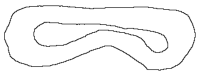
\includegraphics[interpolate=true,width=1.980000in,height=0.730000in]{contents/chapt6/figs/velocity/reward_velocity_controller-img0.png}}%
\end{pgfscope}%
\begin{pgfscope}%
\pgfpathrectangle{\pgfqpoint{0.351458in}{1.090000in}}{\pgfqpoint{1.977083in}{0.730000in}}%
\pgfusepath{clip}%
\pgfsetrectcap%
\pgfsetroundjoin%
\pgfsetlinewidth{1.505625pt}%
\definecolor{currentstroke}{rgb}{0.121569,0.466667,0.705882}%
\pgfsetstrokecolor{currentstroke}%
\pgfsetdash{}{0pt}%
\pgfpathmoveto{\pgfqpoint{1.568125in}{1.637500in}}%
\pgfpathlineto{\pgfqpoint{1.520784in}{1.638442in}}%
\pgfpathlineto{\pgfqpoint{1.481246in}{1.641339in}}%
\pgfpathlineto{\pgfqpoint{1.434359in}{1.647096in}}%
\pgfpathlineto{\pgfqpoint{1.385198in}{1.655353in}}%
\pgfpathlineto{\pgfqpoint{1.308925in}{1.669011in}}%
\pgfpathlineto{\pgfqpoint{1.272286in}{1.672770in}}%
\pgfpathlineto{\pgfqpoint{1.234911in}{1.674301in}}%
\pgfpathlineto{\pgfqpoint{1.191530in}{1.673781in}}%
\pgfpathlineto{\pgfqpoint{1.136884in}{1.670624in}}%
\pgfpathlineto{\pgfqpoint{1.060468in}{1.666543in}}%
\pgfpathlineto{\pgfqpoint{0.887642in}{1.661057in}}%
\pgfpathlineto{\pgfqpoint{0.854064in}{1.656122in}}%
\pgfpathlineto{\pgfqpoint{0.826379in}{1.649797in}}%
\pgfpathlineto{\pgfqpoint{0.804565in}{1.642866in}}%
\pgfpathlineto{\pgfqpoint{0.783284in}{1.634078in}}%
\pgfpathlineto{\pgfqpoint{0.762790in}{1.623328in}}%
\pgfpathlineto{\pgfqpoint{0.743360in}{1.610564in}}%
\pgfpathlineto{\pgfqpoint{0.725267in}{1.595801in}}%
\pgfpathlineto{\pgfqpoint{0.708759in}{1.579124in}}%
\pgfpathlineto{\pgfqpoint{0.694080in}{1.560690in}}%
\pgfpathlineto{\pgfqpoint{0.681448in}{1.540694in}}%
\pgfpathlineto{\pgfqpoint{0.671055in}{1.519362in}}%
\pgfpathlineto{\pgfqpoint{0.663138in}{1.496965in}}%
\pgfpathlineto{\pgfqpoint{0.659133in}{1.479627in}}%
\pgfpathlineto{\pgfqpoint{0.656908in}{1.461994in}}%
\pgfpathlineto{\pgfqpoint{0.656591in}{1.444245in}}%
\pgfpathlineto{\pgfqpoint{0.658268in}{1.426591in}}%
\pgfpathlineto{\pgfqpoint{0.661996in}{1.409273in}}%
\pgfpathlineto{\pgfqpoint{0.667762in}{1.392542in}}%
\pgfpathlineto{\pgfqpoint{0.675551in}{1.376689in}}%
\pgfpathlineto{\pgfqpoint{0.685296in}{1.361997in}}%
\pgfpathlineto{\pgfqpoint{0.696853in}{1.348723in}}%
\pgfpathlineto{\pgfqpoint{0.710053in}{1.337126in}}%
\pgfpathlineto{\pgfqpoint{0.724669in}{1.327425in}}%
\pgfpathlineto{\pgfqpoint{0.740449in}{1.319818in}}%
\pgfpathlineto{\pgfqpoint{0.757104in}{1.314440in}}%
\pgfpathlineto{\pgfqpoint{0.774322in}{1.311267in}}%
\pgfpathlineto{\pgfqpoint{0.791797in}{1.310098in}}%
\pgfpathlineto{\pgfqpoint{0.815126in}{1.311155in}}%
\pgfpathlineto{\pgfqpoint{0.838223in}{1.314667in}}%
\pgfpathlineto{\pgfqpoint{0.866547in}{1.321717in}}%
\pgfpathlineto{\pgfqpoint{0.910211in}{1.335926in}}%
\pgfpathlineto{\pgfqpoint{0.942496in}{1.345669in}}%
\pgfpathlineto{\pgfqpoint{0.969560in}{1.351500in}}%
\pgfpathlineto{\pgfqpoint{0.991533in}{1.354051in}}%
\pgfpathlineto{\pgfqpoint{1.019342in}{1.354884in}}%
\pgfpathlineto{\pgfqpoint{1.069798in}{1.353313in}}%
\pgfpathlineto{\pgfqpoint{1.109147in}{1.352899in}}%
\pgfpathlineto{\pgfqpoint{1.131407in}{1.354638in}}%
\pgfpathlineto{\pgfqpoint{1.153265in}{1.358603in}}%
\pgfpathlineto{\pgfqpoint{1.174375in}{1.365183in}}%
\pgfpathlineto{\pgfqpoint{1.189438in}{1.371979in}}%
\pgfpathlineto{\pgfqpoint{1.203644in}{1.380337in}}%
\pgfpathlineto{\pgfqpoint{1.221155in}{1.393511in}}%
\pgfpathlineto{\pgfqpoint{1.237150in}{1.408402in}}%
\pgfpathlineto{\pgfqpoint{1.263013in}{1.436397in}}%
\pgfpathlineto{\pgfqpoint{1.285504in}{1.459802in}}%
\pgfpathlineto{\pgfqpoint{1.301877in}{1.473636in}}%
\pgfpathlineto{\pgfqpoint{1.315172in}{1.482500in}}%
\pgfpathlineto{\pgfqpoint{1.329326in}{1.489741in}}%
\pgfpathlineto{\pgfqpoint{1.344224in}{1.495068in}}%
\pgfpathlineto{\pgfqpoint{1.359646in}{1.498268in}}%
\pgfpathlineto{\pgfqpoint{1.375453in}{1.499218in}}%
\pgfpathlineto{\pgfqpoint{1.391399in}{1.498066in}}%
\pgfpathlineto{\pgfqpoint{1.407238in}{1.495043in}}%
\pgfpathlineto{\pgfqpoint{1.422773in}{1.490279in}}%
\pgfpathlineto{\pgfqpoint{1.442758in}{1.481490in}}%
\pgfpathlineto{\pgfqpoint{1.461646in}{1.470191in}}%
\pgfpathlineto{\pgfqpoint{1.479133in}{1.456809in}}%
\pgfpathlineto{\pgfqpoint{1.499138in}{1.438067in}}%
\pgfpathlineto{\pgfqpoint{1.556330in}{1.379982in}}%
\pgfpathlineto{\pgfqpoint{1.573572in}{1.367100in}}%
\pgfpathlineto{\pgfqpoint{1.592104in}{1.356360in}}%
\pgfpathlineto{\pgfqpoint{1.611787in}{1.348155in}}%
\pgfpathlineto{\pgfqpoint{1.632326in}{1.342754in}}%
\pgfpathlineto{\pgfqpoint{1.653410in}{1.340248in}}%
\pgfpathlineto{\pgfqpoint{1.674686in}{1.340227in}}%
\pgfpathlineto{\pgfqpoint{1.701221in}{1.342654in}}%
\pgfpathlineto{\pgfqpoint{1.759604in}{1.349132in}}%
\pgfpathlineto{\pgfqpoint{1.780969in}{1.348791in}}%
\pgfpathlineto{\pgfqpoint{1.796864in}{1.346727in}}%
\pgfpathlineto{\pgfqpoint{1.812425in}{1.342894in}}%
\pgfpathlineto{\pgfqpoint{1.827387in}{1.337154in}}%
\pgfpathlineto{\pgfqpoint{1.841456in}{1.329485in}}%
\pgfpathlineto{\pgfqpoint{1.854452in}{1.319878in}}%
\pgfpathlineto{\pgfqpoint{1.866277in}{1.308583in}}%
\pgfpathlineto{\pgfqpoint{1.880231in}{1.291489in}}%
\pgfpathlineto{\pgfqpoint{1.892417in}{1.272761in}}%
\pgfpathlineto{\pgfqpoint{1.911471in}{1.238014in}}%
\pgfpathlineto{\pgfqpoint{1.928295in}{1.208936in}}%
\pgfpathlineto{\pgfqpoint{1.941351in}{1.191213in}}%
\pgfpathlineto{\pgfqpoint{1.952503in}{1.179284in}}%
\pgfpathlineto{\pgfqpoint{1.964910in}{1.168899in}}%
\pgfpathlineto{\pgfqpoint{1.978500in}{1.160378in}}%
\pgfpathlineto{\pgfqpoint{1.993110in}{1.154005in}}%
\pgfpathlineto{\pgfqpoint{2.008451in}{1.149972in}}%
\pgfpathlineto{\pgfqpoint{2.024162in}{1.148406in}}%
\pgfpathlineto{\pgfqpoint{2.039855in}{1.149327in}}%
\pgfpathlineto{\pgfqpoint{2.055143in}{1.152700in}}%
\pgfpathlineto{\pgfqpoint{2.069655in}{1.158405in}}%
\pgfpathlineto{\pgfqpoint{2.083056in}{1.166290in}}%
\pgfpathlineto{\pgfqpoint{2.095145in}{1.176130in}}%
\pgfpathlineto{\pgfqpoint{2.105848in}{1.187526in}}%
\pgfpathlineto{\pgfqpoint{2.118076in}{1.204483in}}%
\pgfpathlineto{\pgfqpoint{2.128414in}{1.222736in}}%
\pgfpathlineto{\pgfqpoint{2.139482in}{1.246594in}}%
\pgfpathlineto{\pgfqpoint{2.152803in}{1.280851in}}%
\pgfpathlineto{\pgfqpoint{2.171205in}{1.335234in}}%
\pgfpathlineto{\pgfqpoint{2.184511in}{1.379627in}}%
\pgfpathlineto{\pgfqpoint{2.189713in}{1.404327in}}%
\pgfpathlineto{\pgfqpoint{2.191540in}{1.424201in}}%
\pgfpathlineto{\pgfqpoint{2.190619in}{1.443943in}}%
\pgfpathlineto{\pgfqpoint{2.187874in}{1.458597in}}%
\pgfpathlineto{\pgfqpoint{2.181627in}{1.477763in}}%
\pgfpathlineto{\pgfqpoint{2.172765in}{1.496192in}}%
\pgfpathlineto{\pgfqpoint{2.161553in}{1.513597in}}%
\pgfpathlineto{\pgfqpoint{2.148253in}{1.529756in}}%
\pgfpathlineto{\pgfqpoint{2.133063in}{1.544548in}}%
\pgfpathlineto{\pgfqpoint{2.112016in}{1.561475in}}%
\pgfpathlineto{\pgfqpoint{2.080298in}{1.583492in}}%
\pgfpathlineto{\pgfqpoint{2.027824in}{1.616720in}}%
\pgfpathlineto{\pgfqpoint{1.997668in}{1.633252in}}%
\pgfpathlineto{\pgfqpoint{1.971337in}{1.645094in}}%
\pgfpathlineto{\pgfqpoint{1.949441in}{1.652822in}}%
\pgfpathlineto{\pgfqpoint{1.921198in}{1.660220in}}%
\pgfpathlineto{\pgfqpoint{1.892251in}{1.665196in}}%
\pgfpathlineto{\pgfqpoint{1.862853in}{1.667887in}}%
\pgfpathlineto{\pgfqpoint{1.833213in}{1.668444in}}%
\pgfpathlineto{\pgfqpoint{1.791690in}{1.666422in}}%
\pgfpathlineto{\pgfqpoint{1.661273in}{1.657626in}}%
\pgfpathlineto{\pgfqpoint{1.619802in}{1.658255in}}%
\pgfpathlineto{\pgfqpoint{1.607981in}{1.658911in}}%
\pgfpathlineto{\pgfqpoint{1.607981in}{1.658911in}}%
\pgfusepath{stroke}%
\end{pgfscope}%
\begin{pgfscope}%
\pgfpathrectangle{\pgfqpoint{0.351458in}{1.090000in}}{\pgfqpoint{1.977083in}{0.730000in}}%
\pgfusepath{clip}%
\pgfsetrectcap%
\pgfsetroundjoin%
\pgfsetlinewidth{1.505625pt}%
\definecolor{currentstroke}{rgb}{1.000000,0.498039,0.054902}%
\pgfsetstrokecolor{currentstroke}%
\pgfsetdash{}{0pt}%
\pgfpathmoveto{\pgfqpoint{1.568125in}{1.637500in}}%
\pgfpathlineto{\pgfqpoint{1.471626in}{1.638577in}}%
\pgfpathlineto{\pgfqpoint{1.383779in}{1.641720in}}%
\pgfpathlineto{\pgfqpoint{1.300722in}{1.646737in}}%
\pgfpathlineto{\pgfqpoint{1.215241in}{1.654096in}}%
\pgfpathlineto{\pgfqpoint{1.112815in}{1.665453in}}%
\pgfpathlineto{\pgfqpoint{1.015553in}{1.675126in}}%
\pgfpathlineto{\pgfqpoint{0.934509in}{1.680793in}}%
\pgfpathlineto{\pgfqpoint{0.902481in}{1.681218in}}%
\pgfpathlineto{\pgfqpoint{0.876118in}{1.679489in}}%
\pgfpathlineto{\pgfqpoint{0.850259in}{1.675312in}}%
\pgfpathlineto{\pgfqpoint{0.825085in}{1.668598in}}%
\pgfpathlineto{\pgfqpoint{0.790802in}{1.656590in}}%
\pgfpathlineto{\pgfqpoint{0.709116in}{1.624396in}}%
\pgfpathlineto{\pgfqpoint{0.685719in}{1.613352in}}%
\pgfpathlineto{\pgfqpoint{0.663403in}{1.600208in}}%
\pgfpathlineto{\pgfqpoint{0.646711in}{1.587826in}}%
\pgfpathlineto{\pgfqpoint{0.631559in}{1.573433in}}%
\pgfpathlineto{\pgfqpoint{0.621538in}{1.561283in}}%
\pgfpathlineto{\pgfqpoint{0.612885in}{1.548059in}}%
\pgfpathlineto{\pgfqpoint{0.605812in}{1.533873in}}%
\pgfpathlineto{\pgfqpoint{0.600488in}{1.518895in}}%
\pgfpathlineto{\pgfqpoint{0.597038in}{1.503291in}}%
\pgfpathlineto{\pgfqpoint{0.595482in}{1.487223in}}%
\pgfpathlineto{\pgfqpoint{0.595844in}{1.470937in}}%
\pgfpathlineto{\pgfqpoint{0.598125in}{1.454673in}}%
\pgfpathlineto{\pgfqpoint{0.602287in}{1.438661in}}%
\pgfpathlineto{\pgfqpoint{0.608298in}{1.423129in}}%
\pgfpathlineto{\pgfqpoint{0.616095in}{1.408300in}}%
\pgfpathlineto{\pgfqpoint{0.625551in}{1.394455in}}%
\pgfpathlineto{\pgfqpoint{0.636408in}{1.381714in}}%
\pgfpathlineto{\pgfqpoint{0.652703in}{1.366532in}}%
\pgfpathlineto{\pgfqpoint{0.670761in}{1.353568in}}%
\pgfpathlineto{\pgfqpoint{0.690198in}{1.342860in}}%
\pgfpathlineto{\pgfqpoint{0.710654in}{1.334385in}}%
\pgfpathlineto{\pgfqpoint{0.737007in}{1.326402in}}%
\pgfpathlineto{\pgfqpoint{0.769127in}{1.319536in}}%
\pgfpathlineto{\pgfqpoint{0.806795in}{1.313954in}}%
\pgfpathlineto{\pgfqpoint{0.850328in}{1.309595in}}%
\pgfpathlineto{\pgfqpoint{0.888996in}{1.307687in}}%
\pgfpathlineto{\pgfqpoint{0.927960in}{1.307853in}}%
\pgfpathlineto{\pgfqpoint{0.971640in}{1.310453in}}%
\pgfpathlineto{\pgfqpoint{1.014131in}{1.315451in}}%
\pgfpathlineto{\pgfqpoint{1.055473in}{1.322761in}}%
\pgfpathlineto{\pgfqpoint{1.090687in}{1.331280in}}%
\pgfpathlineto{\pgfqpoint{1.124899in}{1.341887in}}%
\pgfpathlineto{\pgfqpoint{1.163099in}{1.356403in}}%
\pgfpathlineto{\pgfqpoint{1.200615in}{1.373029in}}%
\pgfpathlineto{\pgfqpoint{1.250736in}{1.398099in}}%
\pgfpathlineto{\pgfqpoint{1.282149in}{1.412615in}}%
\pgfpathlineto{\pgfqpoint{1.309419in}{1.422630in}}%
\pgfpathlineto{\pgfqpoint{1.332439in}{1.428513in}}%
\pgfpathlineto{\pgfqpoint{1.350948in}{1.431242in}}%
\pgfpathlineto{\pgfqpoint{1.369389in}{1.432100in}}%
\pgfpathlineto{\pgfqpoint{1.387592in}{1.431040in}}%
\pgfpathlineto{\pgfqpoint{1.405400in}{1.428073in}}%
\pgfpathlineto{\pgfqpoint{1.427420in}{1.421899in}}%
\pgfpathlineto{\pgfqpoint{1.462556in}{1.409019in}}%
\pgfpathlineto{\pgfqpoint{1.626487in}{1.344432in}}%
\pgfpathlineto{\pgfqpoint{1.658639in}{1.328399in}}%
\pgfpathlineto{\pgfqpoint{1.685680in}{1.312651in}}%
\pgfpathlineto{\pgfqpoint{1.730714in}{1.283361in}}%
\pgfpathlineto{\pgfqpoint{1.805395in}{1.234642in}}%
\pgfpathlineto{\pgfqpoint{1.830805in}{1.221568in}}%
\pgfpathlineto{\pgfqpoint{1.852236in}{1.213071in}}%
\pgfpathlineto{\pgfqpoint{1.874594in}{1.206872in}}%
\pgfpathlineto{\pgfqpoint{1.891869in}{1.204111in}}%
\pgfpathlineto{\pgfqpoint{1.909404in}{1.203152in}}%
\pgfpathlineto{\pgfqpoint{1.927000in}{1.204136in}}%
\pgfpathlineto{\pgfqpoint{1.944422in}{1.207143in}}%
\pgfpathlineto{\pgfqpoint{1.961409in}{1.212224in}}%
\pgfpathlineto{\pgfqpoint{1.977693in}{1.219356in}}%
\pgfpathlineto{\pgfqpoint{1.992973in}{1.228449in}}%
\pgfpathlineto{\pgfqpoint{2.007090in}{1.239239in}}%
\pgfpathlineto{\pgfqpoint{2.019908in}{1.251521in}}%
\pgfpathlineto{\pgfqpoint{2.031306in}{1.265113in}}%
\pgfpathlineto{\pgfqpoint{2.041208in}{1.279816in}}%
\pgfpathlineto{\pgfqpoint{2.049580in}{1.295428in}}%
\pgfpathlineto{\pgfqpoint{2.056387in}{1.311767in}}%
\pgfpathlineto{\pgfqpoint{2.061612in}{1.328640in}}%
\pgfpathlineto{\pgfqpoint{2.066078in}{1.351697in}}%
\pgfpathlineto{\pgfqpoint{2.067670in}{1.375066in}}%
\pgfpathlineto{\pgfqpoint{2.066392in}{1.398396in}}%
\pgfpathlineto{\pgfqpoint{2.062290in}{1.421344in}}%
\pgfpathlineto{\pgfqpoint{2.055456in}{1.443549in}}%
\pgfpathlineto{\pgfqpoint{2.046010in}{1.464677in}}%
\pgfpathlineto{\pgfqpoint{2.034102in}{1.484425in}}%
\pgfpathlineto{\pgfqpoint{2.019923in}{1.502514in}}%
\pgfpathlineto{\pgfqpoint{2.003698in}{1.518692in}}%
\pgfpathlineto{\pgfqpoint{1.985748in}{1.532763in}}%
\pgfpathlineto{\pgfqpoint{1.966529in}{1.544816in}}%
\pgfpathlineto{\pgfqpoint{1.946312in}{1.554856in}}%
\pgfpathlineto{\pgfqpoint{1.925359in}{1.562969in}}%
\pgfpathlineto{\pgfqpoint{1.903889in}{1.569253in}}%
\pgfpathlineto{\pgfqpoint{1.876561in}{1.574915in}}%
\pgfpathlineto{\pgfqpoint{1.837913in}{1.580406in}}%
\pgfpathlineto{\pgfqpoint{1.682831in}{1.599052in}}%
\pgfpathlineto{\pgfqpoint{1.611011in}{1.612552in}}%
\pgfpathlineto{\pgfqpoint{1.577722in}{1.619043in}}%
\pgfpathlineto{\pgfqpoint{1.577722in}{1.619043in}}%
\pgfusepath{stroke}%
\end{pgfscope}%
\begin{pgfscope}%
\pgfpathrectangle{\pgfqpoint{0.351458in}{0.180000in}}{\pgfqpoint{1.977083in}{0.730000in}}%
\pgfusepath{clip}%
\pgfsys@transformshift{0.351458in}{0.180000in}%
\pgftext[left,bottom]{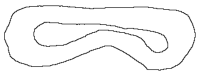
\includegraphics[interpolate=true,width=1.980000in,height=0.730000in]{contents/chapt6/figs/velocity/reward_velocity_controller-img1.png}}%
\end{pgfscope}%
\begin{pgfscope}%
\pgfpathrectangle{\pgfqpoint{0.351458in}{0.180000in}}{\pgfqpoint{1.977083in}{0.730000in}}%
\pgfusepath{clip}%
\pgfsetrectcap%
\pgfsetroundjoin%
\pgfsetlinewidth{1.505625pt}%
\definecolor{currentstroke}{rgb}{0.172549,0.627451,0.172549}%
\pgfsetstrokecolor{currentstroke}%
\pgfsetdash{}{0pt}%
\pgfpathmoveto{\pgfqpoint{1.568125in}{0.727500in}}%
\pgfpathlineto{\pgfqpoint{1.507197in}{0.728570in}}%
\pgfpathlineto{\pgfqpoint{1.451355in}{0.731868in}}%
\pgfpathlineto{\pgfqpoint{1.376716in}{0.738485in}}%
\pgfpathlineto{\pgfqpoint{1.247297in}{0.750153in}}%
\pgfpathlineto{\pgfqpoint{1.167813in}{0.754966in}}%
\pgfpathlineto{\pgfqpoint{1.081283in}{0.757878in}}%
\pgfpathlineto{\pgfqpoint{0.998055in}{0.758437in}}%
\pgfpathlineto{\pgfqpoint{0.918136in}{0.756815in}}%
\pgfpathlineto{\pgfqpoint{0.871741in}{0.753690in}}%
\pgfpathlineto{\pgfqpoint{0.830984in}{0.748733in}}%
\pgfpathlineto{\pgfqpoint{0.802147in}{0.743479in}}%
\pgfpathlineto{\pgfqpoint{0.779554in}{0.737482in}}%
\pgfpathlineto{\pgfqpoint{0.757715in}{0.729321in}}%
\pgfpathlineto{\pgfqpoint{0.742072in}{0.721583in}}%
\pgfpathlineto{\pgfqpoint{0.727301in}{0.712343in}}%
\pgfpathlineto{\pgfqpoint{0.713577in}{0.701546in}}%
\pgfpathlineto{\pgfqpoint{0.701104in}{0.689226in}}%
\pgfpathlineto{\pgfqpoint{0.690073in}{0.675519in}}%
\pgfpathlineto{\pgfqpoint{0.680661in}{0.660586in}}%
\pgfpathlineto{\pgfqpoint{0.673004in}{0.644625in}}%
\pgfpathlineto{\pgfqpoint{0.667231in}{0.627839in}}%
\pgfpathlineto{\pgfqpoint{0.663431in}{0.610457in}}%
\pgfpathlineto{\pgfqpoint{0.661574in}{0.592726in}}%
\pgfpathlineto{\pgfqpoint{0.661639in}{0.574868in}}%
\pgfpathlineto{\pgfqpoint{0.663614in}{0.557091in}}%
\pgfpathlineto{\pgfqpoint{0.667432in}{0.539591in}}%
\pgfpathlineto{\pgfqpoint{0.673032in}{0.522553in}}%
\pgfpathlineto{\pgfqpoint{0.680325in}{0.506145in}}%
\pgfpathlineto{\pgfqpoint{0.689236in}{0.490532in}}%
\pgfpathlineto{\pgfqpoint{0.699664in}{0.475858in}}%
\pgfpathlineto{\pgfqpoint{0.711510in}{0.462274in}}%
\pgfpathlineto{\pgfqpoint{0.724650in}{0.449908in}}%
\pgfpathlineto{\pgfqpoint{0.738964in}{0.438892in}}%
\pgfpathlineto{\pgfqpoint{0.754307in}{0.429330in}}%
\pgfpathlineto{\pgfqpoint{0.770536in}{0.421330in}}%
\pgfpathlineto{\pgfqpoint{0.793231in}{0.413102in}}%
\pgfpathlineto{\pgfqpoint{0.816714in}{0.407416in}}%
\pgfpathlineto{\pgfqpoint{0.840674in}{0.404150in}}%
\pgfpathlineto{\pgfqpoint{0.864849in}{0.403102in}}%
\pgfpathlineto{\pgfqpoint{0.889041in}{0.404086in}}%
\pgfpathlineto{\pgfqpoint{0.919104in}{0.407724in}}%
\pgfpathlineto{\pgfqpoint{0.954822in}{0.414532in}}%
\pgfpathlineto{\pgfqpoint{1.001886in}{0.426296in}}%
\pgfpathlineto{\pgfqpoint{1.111909in}{0.457759in}}%
\pgfpathlineto{\pgfqpoint{1.198120in}{0.480982in}}%
\pgfpathlineto{\pgfqpoint{1.272785in}{0.498740in}}%
\pgfpathlineto{\pgfqpoint{1.318942in}{0.507330in}}%
\pgfpathlineto{\pgfqpoint{1.359541in}{0.512485in}}%
\pgfpathlineto{\pgfqpoint{1.388572in}{0.514322in}}%
\pgfpathlineto{\pgfqpoint{1.417518in}{0.513830in}}%
\pgfpathlineto{\pgfqpoint{1.440467in}{0.511462in}}%
\pgfpathlineto{\pgfqpoint{1.463049in}{0.507117in}}%
\pgfpathlineto{\pgfqpoint{1.485156in}{0.500708in}}%
\pgfpathlineto{\pgfqpoint{1.512242in}{0.490368in}}%
\pgfpathlineto{\pgfqpoint{1.544050in}{0.475601in}}%
\pgfpathlineto{\pgfqpoint{1.585730in}{0.453572in}}%
\pgfpathlineto{\pgfqpoint{1.669810in}{0.408836in}}%
\pgfpathlineto{\pgfqpoint{1.718573in}{0.385716in}}%
\pgfpathlineto{\pgfqpoint{1.779374in}{0.359486in}}%
\pgfpathlineto{\pgfqpoint{1.829944in}{0.339623in}}%
\pgfpathlineto{\pgfqpoint{1.858747in}{0.330451in}}%
\pgfpathlineto{\pgfqpoint{1.888197in}{0.323533in}}%
\pgfpathlineto{\pgfqpoint{1.912171in}{0.320098in}}%
\pgfpathlineto{\pgfqpoint{1.936371in}{0.318944in}}%
\pgfpathlineto{\pgfqpoint{1.960555in}{0.320531in}}%
\pgfpathlineto{\pgfqpoint{1.978474in}{0.323649in}}%
\pgfpathlineto{\pgfqpoint{1.996005in}{0.328512in}}%
\pgfpathlineto{\pgfqpoint{2.012950in}{0.335144in}}%
\pgfpathlineto{\pgfqpoint{2.029092in}{0.343539in}}%
\pgfpathlineto{\pgfqpoint{2.044195in}{0.353614in}}%
\pgfpathlineto{\pgfqpoint{2.058046in}{0.365284in}}%
\pgfpathlineto{\pgfqpoint{2.070457in}{0.378419in}}%
\pgfpathlineto{\pgfqpoint{2.081244in}{0.392869in}}%
\pgfpathlineto{\pgfqpoint{2.090264in}{0.408442in}}%
\pgfpathlineto{\pgfqpoint{2.097382in}{0.424934in}}%
\pgfpathlineto{\pgfqpoint{2.102517in}{0.442123in}}%
\pgfpathlineto{\pgfqpoint{2.105601in}{0.459793in}}%
\pgfpathlineto{\pgfqpoint{2.106617in}{0.477698in}}%
\pgfpathlineto{\pgfqpoint{2.105556in}{0.495598in}}%
\pgfpathlineto{\pgfqpoint{2.102457in}{0.513256in}}%
\pgfpathlineto{\pgfqpoint{2.097361in}{0.530443in}}%
\pgfpathlineto{\pgfqpoint{2.090351in}{0.546939in}}%
\pgfpathlineto{\pgfqpoint{2.081555in}{0.562494in}}%
\pgfpathlineto{\pgfqpoint{2.071255in}{0.577005in}}%
\pgfpathlineto{\pgfqpoint{2.055593in}{0.594670in}}%
\pgfpathlineto{\pgfqpoint{2.038077in}{0.610323in}}%
\pgfpathlineto{\pgfqpoint{2.019115in}{0.624004in}}%
\pgfpathlineto{\pgfqpoint{1.999043in}{0.635818in}}%
\pgfpathlineto{\pgfqpoint{1.972945in}{0.648555in}}%
\pgfpathlineto{\pgfqpoint{1.940761in}{0.661672in}}%
\pgfpathlineto{\pgfqpoint{1.897144in}{0.676869in}}%
\pgfpathlineto{\pgfqpoint{1.848001in}{0.691730in}}%
\pgfpathlineto{\pgfqpoint{1.798963in}{0.704132in}}%
\pgfpathlineto{\pgfqpoint{1.755414in}{0.712917in}}%
\pgfpathlineto{\pgfqpoint{1.711914in}{0.719546in}}%
\pgfpathlineto{\pgfqpoint{1.668485in}{0.724051in}}%
\pgfpathlineto{\pgfqpoint{1.625015in}{0.726502in}}%
\pgfpathlineto{\pgfqpoint{1.581548in}{0.726957in}}%
\pgfpathlineto{\pgfqpoint{1.581548in}{0.726957in}}%
\pgfusepath{stroke}%
\end{pgfscope}%
\begin{pgfscope}%
\pgfpathrectangle{\pgfqpoint{0.351458in}{0.180000in}}{\pgfqpoint{1.977083in}{0.730000in}}%
\pgfusepath{clip}%
\pgfsetrectcap%
\pgfsetroundjoin%
\pgfsetlinewidth{1.505625pt}%
\definecolor{currentstroke}{rgb}{0.839216,0.152941,0.156863}%
\pgfsetstrokecolor{currentstroke}%
\pgfsetdash{}{0pt}%
\pgfpathmoveto{\pgfqpoint{1.568125in}{0.727500in}}%
\pgfpathlineto{\pgfqpoint{1.526707in}{0.728485in}}%
\pgfpathlineto{\pgfqpoint{1.495242in}{0.731453in}}%
\pgfpathlineto{\pgfqpoint{1.454528in}{0.738020in}}%
\pgfpathlineto{\pgfqpoint{1.407263in}{0.744888in}}%
\pgfpathlineto{\pgfqpoint{1.366994in}{0.748349in}}%
\pgfpathlineto{\pgfqpoint{1.330351in}{0.749279in}}%
\pgfpathlineto{\pgfqpoint{1.288682in}{0.747918in}}%
\pgfpathlineto{\pgfqpoint{1.242670in}{0.746936in}}%
\pgfpathlineto{\pgfqpoint{1.210667in}{0.748356in}}%
\pgfpathlineto{\pgfqpoint{1.164930in}{0.753176in}}%
\pgfpathlineto{\pgfqpoint{1.043548in}{0.768080in}}%
\pgfpathlineto{\pgfqpoint{0.995274in}{0.769899in}}%
\pgfpathlineto{\pgfqpoint{0.892911in}{0.771276in}}%
\pgfpathlineto{\pgfqpoint{0.862656in}{0.768868in}}%
\pgfpathlineto{\pgfqpoint{0.837354in}{0.764550in}}%
\pgfpathlineto{\pgfqpoint{0.812153in}{0.757688in}}%
\pgfpathlineto{\pgfqpoint{0.792272in}{0.750162in}}%
\pgfpathlineto{\pgfqpoint{0.772886in}{0.740786in}}%
\pgfpathlineto{\pgfqpoint{0.754232in}{0.729549in}}%
\pgfpathlineto{\pgfqpoint{0.736547in}{0.716472in}}%
\pgfpathlineto{\pgfqpoint{0.719961in}{0.701697in}}%
\pgfpathlineto{\pgfqpoint{0.700779in}{0.681247in}}%
\pgfpathlineto{\pgfqpoint{0.683412in}{0.658899in}}%
\pgfpathlineto{\pgfqpoint{0.667906in}{0.634953in}}%
\pgfpathlineto{\pgfqpoint{0.654514in}{0.609712in}}%
\pgfpathlineto{\pgfqpoint{0.645939in}{0.588562in}}%
\pgfpathlineto{\pgfqpoint{0.639666in}{0.566652in}}%
\pgfpathlineto{\pgfqpoint{0.636054in}{0.544180in}}%
\pgfpathlineto{\pgfqpoint{0.635272in}{0.527140in}}%
\pgfpathlineto{\pgfqpoint{0.636299in}{0.510136in}}%
\pgfpathlineto{\pgfqpoint{0.639262in}{0.493383in}}%
\pgfpathlineto{\pgfqpoint{0.644188in}{0.477122in}}%
\pgfpathlineto{\pgfqpoint{0.651057in}{0.461605in}}%
\pgfpathlineto{\pgfqpoint{0.659825in}{0.447099in}}%
\pgfpathlineto{\pgfqpoint{0.670372in}{0.433853in}}%
\pgfpathlineto{\pgfqpoint{0.682536in}{0.422125in}}%
\pgfpathlineto{\pgfqpoint{0.695985in}{0.412143in}}%
\pgfpathlineto{\pgfqpoint{0.710384in}{0.403902in}}%
\pgfpathlineto{\pgfqpoint{0.725464in}{0.397352in}}%
\pgfpathlineto{\pgfqpoint{0.746280in}{0.391232in}}%
\pgfpathlineto{\pgfqpoint{0.767485in}{0.387891in}}%
\pgfpathlineto{\pgfqpoint{0.788700in}{0.387061in}}%
\pgfpathlineto{\pgfqpoint{0.814759in}{0.388775in}}%
\pgfpathlineto{\pgfqpoint{0.850212in}{0.393975in}}%
\pgfpathlineto{\pgfqpoint{0.923641in}{0.408033in}}%
\pgfpathlineto{\pgfqpoint{0.966805in}{0.418280in}}%
\pgfpathlineto{\pgfqpoint{1.004424in}{0.429476in}}%
\pgfpathlineto{\pgfqpoint{1.045897in}{0.444261in}}%
\pgfpathlineto{\pgfqpoint{1.091025in}{0.462970in}}%
\pgfpathlineto{\pgfqpoint{1.159045in}{0.491207in}}%
\pgfpathlineto{\pgfqpoint{1.196088in}{0.504439in}}%
\pgfpathlineto{\pgfqpoint{1.233771in}{0.515482in}}%
\pgfpathlineto{\pgfqpoint{1.267153in}{0.523061in}}%
\pgfpathlineto{\pgfqpoint{1.290971in}{0.526633in}}%
\pgfpathlineto{\pgfqpoint{1.314690in}{0.528119in}}%
\pgfpathlineto{\pgfqpoint{1.338147in}{0.527236in}}%
\pgfpathlineto{\pgfqpoint{1.361161in}{0.523894in}}%
\pgfpathlineto{\pgfqpoint{1.392748in}{0.516497in}}%
\pgfpathlineto{\pgfqpoint{1.437681in}{0.505985in}}%
\pgfpathlineto{\pgfqpoint{1.478568in}{0.499298in}}%
\pgfpathlineto{\pgfqpoint{1.533393in}{0.492963in}}%
\pgfpathlineto{\pgfqpoint{1.582870in}{0.486927in}}%
\pgfpathlineto{\pgfqpoint{1.617926in}{0.480639in}}%
\pgfpathlineto{\pgfqpoint{1.648080in}{0.473059in}}%
\pgfpathlineto{\pgfqpoint{1.673377in}{0.464238in}}%
\pgfpathlineto{\pgfqpoint{1.697837in}{0.453054in}}%
\pgfpathlineto{\pgfqpoint{1.721534in}{0.439366in}}%
\pgfpathlineto{\pgfqpoint{1.748871in}{0.420810in}}%
\pgfpathlineto{\pgfqpoint{1.775791in}{0.400030in}}%
\pgfpathlineto{\pgfqpoint{1.837506in}{0.350240in}}%
\pgfpathlineto{\pgfqpoint{1.858583in}{0.336860in}}%
\pgfpathlineto{\pgfqpoint{1.876233in}{0.327690in}}%
\pgfpathlineto{\pgfqpoint{1.894612in}{0.320510in}}%
\pgfpathlineto{\pgfqpoint{1.913585in}{0.315650in}}%
\pgfpathlineto{\pgfqpoint{1.932901in}{0.313374in}}%
\pgfpathlineto{\pgfqpoint{1.952220in}{0.313852in}}%
\pgfpathlineto{\pgfqpoint{1.971172in}{0.317001in}}%
\pgfpathlineto{\pgfqpoint{1.989539in}{0.322271in}}%
\pgfpathlineto{\pgfqpoint{2.011687in}{0.330836in}}%
\pgfpathlineto{\pgfqpoint{2.041498in}{0.345012in}}%
\pgfpathlineto{\pgfqpoint{2.071268in}{0.361264in}}%
\pgfpathlineto{\pgfqpoint{2.092356in}{0.375010in}}%
\pgfpathlineto{\pgfqpoint{2.108399in}{0.387956in}}%
\pgfpathlineto{\pgfqpoint{2.123138in}{0.402891in}}%
\pgfpathlineto{\pgfqpoint{2.132885in}{0.415329in}}%
\pgfpathlineto{\pgfqpoint{2.141137in}{0.428747in}}%
\pgfpathlineto{\pgfqpoint{2.147643in}{0.443041in}}%
\pgfpathlineto{\pgfqpoint{2.152189in}{0.458028in}}%
\pgfpathlineto{\pgfqpoint{2.154594in}{0.473461in}}%
\pgfpathlineto{\pgfqpoint{2.154765in}{0.489041in}}%
\pgfpathlineto{\pgfqpoint{2.152657in}{0.504439in}}%
\pgfpathlineto{\pgfqpoint{2.148353in}{0.519316in}}%
\pgfpathlineto{\pgfqpoint{2.141979in}{0.533371in}}%
\pgfpathlineto{\pgfqpoint{2.133670in}{0.546315in}}%
\pgfpathlineto{\pgfqpoint{2.123629in}{0.557903in}}%
\pgfpathlineto{\pgfqpoint{2.112076in}{0.567916in}}%
\pgfpathlineto{\pgfqpoint{2.099268in}{0.576184in}}%
\pgfpathlineto{\pgfqpoint{2.085502in}{0.582566in}}%
\pgfpathlineto{\pgfqpoint{2.071164in}{0.587125in}}%
\pgfpathlineto{\pgfqpoint{2.051620in}{0.590689in}}%
\pgfpathlineto{\pgfqpoint{2.031993in}{0.592003in}}%
\pgfpathlineto{\pgfqpoint{1.959928in}{0.593630in}}%
\pgfpathlineto{\pgfqpoint{1.941555in}{0.597686in}}%
\pgfpathlineto{\pgfqpoint{1.924150in}{0.604404in}}%
\pgfpathlineto{\pgfqpoint{1.912056in}{0.611264in}}%
\pgfpathlineto{\pgfqpoint{1.901056in}{0.619606in}}%
\pgfpathlineto{\pgfqpoint{1.888330in}{0.632612in}}%
\pgfpathlineto{\pgfqpoint{1.877735in}{0.647141in}}%
\pgfpathlineto{\pgfqpoint{1.866870in}{0.666497in}}%
\pgfpathlineto{\pgfqpoint{1.836767in}{0.724855in}}%
\pgfpathlineto{\pgfqpoint{1.826025in}{0.738791in}}%
\pgfpathlineto{\pgfqpoint{1.813468in}{0.751168in}}%
\pgfpathlineto{\pgfqpoint{1.799186in}{0.761526in}}%
\pgfpathlineto{\pgfqpoint{1.783496in}{0.769430in}}%
\pgfpathlineto{\pgfqpoint{1.766777in}{0.774581in}}%
\pgfpathlineto{\pgfqpoint{1.753840in}{0.776518in}}%
\pgfpathlineto{\pgfqpoint{1.740796in}{0.776769in}}%
\pgfpathlineto{\pgfqpoint{1.727865in}{0.775325in}}%
\pgfpathlineto{\pgfqpoint{1.715235in}{0.772221in}}%
\pgfpathlineto{\pgfqpoint{1.699051in}{0.765797in}}%
\pgfpathlineto{\pgfqpoint{1.683723in}{0.757371in}}%
\pgfpathlineto{\pgfqpoint{1.662005in}{0.742429in}}%
\pgfpathlineto{\pgfqpoint{1.626070in}{0.717038in}}%
\pgfpathlineto{\pgfqpoint{1.610643in}{0.708870in}}%
\pgfpathlineto{\pgfqpoint{1.594378in}{0.702781in}}%
\pgfpathlineto{\pgfqpoint{1.577473in}{0.699165in}}%
\pgfpathlineto{\pgfqpoint{1.573186in}{0.698686in}}%
\pgfpathlineto{\pgfqpoint{1.573186in}{0.698686in}}%
\pgfusepath{stroke}%
\end{pgfscope}%
\begin{pgfscope}%
\pgfsetbuttcap%
\pgfsetmiterjoin%
\definecolor{currentfill}{rgb}{1.000000,1.000000,1.000000}%
\pgfsetfillcolor{currentfill}%
\pgfsetfillopacity{0.800000}%
\pgfsetlinewidth{1.003750pt}%
\definecolor{currentstroke}{rgb}{0.800000,0.800000,0.800000}%
\pgfsetstrokecolor{currentstroke}%
\pgfsetstrokeopacity{0.800000}%
\pgfsetdash{}{0pt}%
\pgfpathmoveto{\pgfqpoint{2.652684in}{0.326936in}}%
\pgfpathlineto{\pgfqpoint{4.883333in}{0.326936in}}%
\pgfpathquadraticcurveto{\pgfqpoint{4.916667in}{0.326936in}}{\pgfqpoint{4.916667in}{0.360269in}}%
\pgfpathlineto{\pgfqpoint{4.916667in}{1.639731in}}%
\pgfpathquadraticcurveto{\pgfqpoint{4.916667in}{1.673064in}}{\pgfqpoint{4.883333in}{1.673064in}}%
\pgfpathlineto{\pgfqpoint{2.652684in}{1.673064in}}%
\pgfpathquadraticcurveto{\pgfqpoint{2.619350in}{1.673064in}}{\pgfqpoint{2.619350in}{1.639731in}}%
\pgfpathlineto{\pgfqpoint{2.619350in}{0.360269in}}%
\pgfpathquadraticcurveto{\pgfqpoint{2.619350in}{0.326936in}}{\pgfqpoint{2.652684in}{0.326936in}}%
\pgfpathlineto{\pgfqpoint{2.652684in}{0.326936in}}%
\pgfpathclose%
\pgfusepath{stroke,fill}%
\end{pgfscope}%
\begin{pgfscope}%
\definecolor{textcolor}{rgb}{0.000000,0.000000,0.000000}%
\pgfsetstrokecolor{textcolor}%
\pgfsetfillcolor{textcolor}%
\pgftext[x=3.265425in,y=1.490731in,left,base]{\color{textcolor}\rmfamily\fontsize{12.000000}{14.400000}\selectfont Reward signal}%
\end{pgfscope}%
\begin{pgfscope}%
\pgfsetrectcap%
\pgfsetroundjoin%
\pgfsetlinewidth{1.505625pt}%
\definecolor{currentstroke}{rgb}{0.121569,0.466667,0.705882}%
\pgfsetstrokecolor{currentstroke}%
\pgfsetdash{}{0pt}%
\pgfpathmoveto{\pgfqpoint{2.686017in}{1.281564in}}%
\pgfpathlineto{\pgfqpoint{2.852684in}{1.281564in}}%
\pgfpathlineto{\pgfqpoint{3.019350in}{1.281564in}}%
\pgfusepath{stroke}%
\end{pgfscope}%
\begin{pgfscope}%
\definecolor{textcolor}{rgb}{0.000000,0.000000,0.000000}%
\pgfsetstrokecolor{textcolor}%
\pgfsetfillcolor{textcolor}%
\pgftext[x=3.152684in,y=1.223231in,left,base]{\color{textcolor}\rmfamily\fontsize{12.000000}{14.400000}\selectfont \(\displaystyle r_{\mathrm{dist}}=0.3, r_{\mathrm{collision}}=-2\)}%
\end{pgfscope}%
\begin{pgfscope}%
\pgfsetrectcap%
\pgfsetroundjoin%
\pgfsetlinewidth{1.505625pt}%
\definecolor{currentstroke}{rgb}{1.000000,0.498039,0.054902}%
\pgfsetstrokecolor{currentstroke}%
\pgfsetdash{}{0pt}%
\pgfpathmoveto{\pgfqpoint{2.686017in}{1.015824in}}%
\pgfpathlineto{\pgfqpoint{2.852684in}{1.015824in}}%
\pgfpathlineto{\pgfqpoint{3.019350in}{1.015824in}}%
\pgfusepath{stroke}%
\end{pgfscope}%
\begin{pgfscope}%
\definecolor{textcolor}{rgb}{0.000000,0.000000,0.000000}%
\pgfsetstrokecolor{textcolor}%
\pgfsetfillcolor{textcolor}%
\pgftext[x=3.152684in,y=0.957490in,left,base]{\color{textcolor}\rmfamily\fontsize{12.000000}{14.400000}\selectfont \(\displaystyle r_{\mathrm{dist}}=0.3, r_{\mathrm{collision}}=-8\)}%
\end{pgfscope}%
\begin{pgfscope}%
\pgfsetrectcap%
\pgfsetroundjoin%
\pgfsetlinewidth{1.505625pt}%
\definecolor{currentstroke}{rgb}{0.172549,0.627451,0.172549}%
\pgfsetstrokecolor{currentstroke}%
\pgfsetdash{}{0pt}%
\pgfpathmoveto{\pgfqpoint{2.686017in}{0.750083in}}%
\pgfpathlineto{\pgfqpoint{2.852684in}{0.750083in}}%
\pgfpathlineto{\pgfqpoint{3.019350in}{0.750083in}}%
\pgfusepath{stroke}%
\end{pgfscope}%
\begin{pgfscope}%
\definecolor{textcolor}{rgb}{0.000000,0.000000,0.000000}%
\pgfsetstrokecolor{textcolor}%
\pgfsetfillcolor{textcolor}%
\pgftext[x=3.152684in,y=0.691750in,left,base]{\color{textcolor}\rmfamily\fontsize{12.000000}{14.400000}\selectfont \(\displaystyle r_{\mathrm{dist}}=0.2, r_{\mathrm{collision}}=-2\)}%
\end{pgfscope}%
\begin{pgfscope}%
\pgfsetrectcap%
\pgfsetroundjoin%
\pgfsetlinewidth{1.505625pt}%
\definecolor{currentstroke}{rgb}{0.839216,0.152941,0.156863}%
\pgfsetstrokecolor{currentstroke}%
\pgfsetdash{}{0pt}%
\pgfpathmoveto{\pgfqpoint{2.686017in}{0.484343in}}%
\pgfpathlineto{\pgfqpoint{2.852684in}{0.484343in}}%
\pgfpathlineto{\pgfqpoint{3.019350in}{0.484343in}}%
\pgfusepath{stroke}%
\end{pgfscope}%
\begin{pgfscope}%
\definecolor{textcolor}{rgb}{0.000000,0.000000,0.000000}%
\pgfsetstrokecolor{textcolor}%
\pgfsetfillcolor{textcolor}%
\pgftext[x=3.152684in,y=0.426010in,left,base]{\color{textcolor}\rmfamily\fontsize{12.000000}{14.400000}\selectfont \(\displaystyle r_{\mathrm{dist}}=0.2, r_{\mathrm{collision}}=-8\)}%
\end{pgfscope}%
\end{pgfpicture}%
\makeatother%
\endgroup%

%     \caption{Caption}
%     \label{fig:velocity_control_lap_reward}
% \end{figure}

\subsection{Evaluation of an agent with a velocity controller}

The path taken and longitudinal velocity profile of an agent with a velocity controller, as well as an end-to-end agent without velocity control is shown in Figure \ref{fig:velocity_control_lap}.
\begin{figure}[htb!]
    \centering
    %% Creator: Matplotlib, PGF backend
%%
%% To include the figure in your LaTeX document, write
%%   \input{<filename>.pgf}
%%
%% Make sure the required packages are loaded in your preamble
%%   \usepackage{pgf}
%%
%% Also ensure that all the required font packages are loaded; for instance,
%% the lmodern package is sometimes necessary when using math font.
%%   \usepackage{lmodern}
%%
%% Figures using additional raster images can only be included by \input if
%% they are in the same directory as the main LaTeX file. For loading figures
%% from other directories you can use the `import` package
%%   \usepackage{import}
%%
%% and then include the figures with
%%   \import{<path to file>}{<filename>.pgf}
%%
%% Matplotlib used the following preamble
%%   \usepackage{fontspec}
%%
\begingroup%
\makeatletter%
\begin{pgfpicture}%
\pgfpathrectangle{\pgfpointorigin}{\pgfqpoint{5.000000in}{4.000000in}}%
\pgfusepath{use as bounding box, clip}%
\begin{pgfscope}%
\pgfsetbuttcap%
\pgfsetmiterjoin%
\definecolor{currentfill}{rgb}{1.000000,1.000000,1.000000}%
\pgfsetfillcolor{currentfill}%
\pgfsetlinewidth{0.000000pt}%
\definecolor{currentstroke}{rgb}{1.000000,1.000000,1.000000}%
\pgfsetstrokecolor{currentstroke}%
\pgfsetdash{}{0pt}%
\pgfpathmoveto{\pgfqpoint{0.000000in}{0.000000in}}%
\pgfpathlineto{\pgfqpoint{5.000000in}{0.000000in}}%
\pgfpathlineto{\pgfqpoint{5.000000in}{4.000000in}}%
\pgfpathlineto{\pgfqpoint{0.000000in}{4.000000in}}%
\pgfpathlineto{\pgfqpoint{0.000000in}{0.000000in}}%
\pgfpathclose%
\pgfusepath{fill}%
\end{pgfscope}%
\begin{pgfscope}%
\pgfpathrectangle{\pgfqpoint{0.892427in}{2.418303in}}{\pgfqpoint{3.620014in}{1.336620in}}%
\pgfusepath{clip}%
\pgfsys@transformshift{0.892427in}{2.418303in}%
\pgftext[left,bottom]{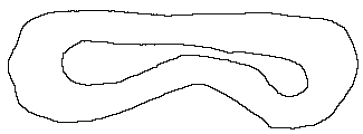
\includegraphics[interpolate=true,width=3.630000in,height=1.340000in]{contents/chapt6/figs/velocity/velocity_control_lap_1-img0.png}}%
\end{pgfscope}%
\begin{pgfscope}%
\pgfpathrectangle{\pgfqpoint{0.892427in}{2.418303in}}{\pgfqpoint{3.620014in}{1.336620in}}%
\pgfusepath{clip}%
\pgfsetrectcap%
\pgfsetroundjoin%
\pgfsetlinewidth{1.505625pt}%
\definecolor{currentstroke}{rgb}{0.121569,0.466667,0.705882}%
\pgfsetstrokecolor{currentstroke}%
\pgfsetdash{}{0pt}%
\pgfpathmoveto{\pgfqpoint{3.120128in}{3.420769in}}%
\pgfpathlineto{\pgfqpoint{3.042008in}{3.421711in}}%
\pgfpathlineto{\pgfqpoint{2.970602in}{3.424768in}}%
\pgfpathlineto{\pgfqpoint{2.882757in}{3.430956in}}%
\pgfpathlineto{\pgfqpoint{2.753900in}{3.442414in}}%
\pgfpathlineto{\pgfqpoint{2.643204in}{3.451772in}}%
\pgfpathlineto{\pgfqpoint{2.564674in}{3.456276in}}%
\pgfpathlineto{\pgfqpoint{2.486043in}{3.458442in}}%
\pgfpathlineto{\pgfqpoint{2.317489in}{3.460055in}}%
\pgfpathlineto{\pgfqpoint{2.092744in}{3.461109in}}%
\pgfpathlineto{\pgfqpoint{2.002865in}{3.459292in}}%
\pgfpathlineto{\pgfqpoint{1.924307in}{3.455325in}}%
\pgfpathlineto{\pgfqpoint{1.857121in}{3.449682in}}%
\pgfpathlineto{\pgfqpoint{1.790166in}{3.441761in}}%
\pgfpathlineto{\pgfqpoint{1.723533in}{3.431479in}}%
\pgfpathlineto{\pgfqpoint{1.657313in}{3.418811in}}%
\pgfpathlineto{\pgfqpoint{1.602612in}{3.405997in}}%
\pgfpathlineto{\pgfqpoint{1.570253in}{3.396552in}}%
\pgfpathlineto{\pgfqpoint{1.538528in}{3.385166in}}%
\pgfpathlineto{\pgfqpoint{1.507721in}{3.371493in}}%
\pgfpathlineto{\pgfqpoint{1.478190in}{3.355254in}}%
\pgfpathlineto{\pgfqpoint{1.459428in}{3.342886in}}%
\pgfpathlineto{\pgfqpoint{1.441566in}{3.329250in}}%
\pgfpathlineto{\pgfqpoint{1.424767in}{3.314326in}}%
\pgfpathlineto{\pgfqpoint{1.409240in}{3.298083in}}%
\pgfpathlineto{\pgfqpoint{1.395129in}{3.280597in}}%
\pgfpathlineto{\pgfqpoint{1.382583in}{3.261955in}}%
\pgfpathlineto{\pgfqpoint{1.371749in}{3.242270in}}%
\pgfpathlineto{\pgfqpoint{1.362762in}{3.221677in}}%
\pgfpathlineto{\pgfqpoint{1.355740in}{3.200333in}}%
\pgfpathlineto{\pgfqpoint{1.350781in}{3.178419in}}%
\pgfpathlineto{\pgfqpoint{1.347958in}{3.156128in}}%
\pgfpathlineto{\pgfqpoint{1.347322in}{3.133669in}}%
\pgfpathlineto{\pgfqpoint{1.348791in}{3.111248in}}%
\pgfpathlineto{\pgfqpoint{1.352236in}{3.089044in}}%
\pgfpathlineto{\pgfqpoint{1.357501in}{3.067199in}}%
\pgfpathlineto{\pgfqpoint{1.364428in}{3.045822in}}%
\pgfpathlineto{\pgfqpoint{1.372916in}{3.025016in}}%
\pgfpathlineto{\pgfqpoint{1.382834in}{3.004851in}}%
\pgfpathlineto{\pgfqpoint{1.400096in}{2.975906in}}%
\pgfpathlineto{\pgfqpoint{1.419868in}{2.948612in}}%
\pgfpathlineto{\pgfqpoint{1.441797in}{2.923016in}}%
\pgfpathlineto{\pgfqpoint{1.465529in}{2.899080in}}%
\pgfpathlineto{\pgfqpoint{1.490844in}{2.876824in}}%
\pgfpathlineto{\pgfqpoint{1.517534in}{2.856238in}}%
\pgfpathlineto{\pgfqpoint{1.545443in}{2.837335in}}%
\pgfpathlineto{\pgfqpoint{1.574414in}{2.820104in}}%
\pgfpathlineto{\pgfqpoint{1.604330in}{2.804570in}}%
\pgfpathlineto{\pgfqpoint{1.635083in}{2.790768in}}%
\pgfpathlineto{\pgfqpoint{1.666605in}{2.778826in}}%
\pgfpathlineto{\pgfqpoint{1.698789in}{2.768807in}}%
\pgfpathlineto{\pgfqpoint{1.731525in}{2.760770in}}%
\pgfpathlineto{\pgfqpoint{1.764700in}{2.754806in}}%
\pgfpathlineto{\pgfqpoint{1.798187in}{2.750958in}}%
\pgfpathlineto{\pgfqpoint{1.831853in}{2.749290in}}%
\pgfpathlineto{\pgfqpoint{1.865559in}{2.749706in}}%
\pgfpathlineto{\pgfqpoint{1.899186in}{2.752042in}}%
\pgfpathlineto{\pgfqpoint{1.932634in}{2.756228in}}%
\pgfpathlineto{\pgfqpoint{1.965815in}{2.762175in}}%
\pgfpathlineto{\pgfqpoint{2.009523in}{2.772636in}}%
\pgfpathlineto{\pgfqpoint{2.052494in}{2.785803in}}%
\pgfpathlineto{\pgfqpoint{2.094688in}{2.801290in}}%
\pgfpathlineto{\pgfqpoint{2.146624in}{2.822722in}}%
\pgfpathlineto{\pgfqpoint{2.218307in}{2.855112in}}%
\pgfpathlineto{\pgfqpoint{2.361394in}{2.920498in}}%
\pgfpathlineto{\pgfqpoint{2.423599in}{2.946505in}}%
\pgfpathlineto{\pgfqpoint{2.486574in}{2.970584in}}%
\pgfpathlineto{\pgfqpoint{2.550332in}{2.992508in}}%
\pgfpathlineto{\pgfqpoint{2.614825in}{3.012163in}}%
\pgfpathlineto{\pgfqpoint{2.679982in}{3.029488in}}%
\pgfpathlineto{\pgfqpoint{2.723839in}{3.039328in}}%
\pgfpathlineto{\pgfqpoint{2.768080in}{3.047257in}}%
\pgfpathlineto{\pgfqpoint{2.812662in}{3.052956in}}%
\pgfpathlineto{\pgfqpoint{2.857498in}{3.056065in}}%
\pgfpathlineto{\pgfqpoint{2.902428in}{3.056313in}}%
\pgfpathlineto{\pgfqpoint{2.947144in}{3.053877in}}%
\pgfpathlineto{\pgfqpoint{2.991460in}{3.048894in}}%
\pgfpathlineto{\pgfqpoint{3.035254in}{3.041519in}}%
\pgfpathlineto{\pgfqpoint{3.078433in}{3.031955in}}%
\pgfpathlineto{\pgfqpoint{3.120889in}{3.020389in}}%
\pgfpathlineto{\pgfqpoint{3.162099in}{3.006938in}}%
\pgfpathlineto{\pgfqpoint{3.201821in}{2.991581in}}%
\pgfpathlineto{\pgfqpoint{3.239903in}{2.974284in}}%
\pgfpathlineto{\pgfqpoint{3.276174in}{2.955032in}}%
\pgfpathlineto{\pgfqpoint{3.310466in}{2.933885in}}%
\pgfpathlineto{\pgfqpoint{3.342596in}{2.911176in}}%
\pgfpathlineto{\pgfqpoint{3.372515in}{2.887169in}}%
\pgfpathlineto{\pgfqpoint{3.400215in}{2.862080in}}%
\pgfpathlineto{\pgfqpoint{3.425743in}{2.836148in}}%
\pgfpathlineto{\pgfqpoint{3.449233in}{2.809512in}}%
\pgfpathlineto{\pgfqpoint{3.532537in}{2.710393in}}%
\pgfpathlineto{\pgfqpoint{3.560313in}{2.683270in}}%
\pgfpathlineto{\pgfqpoint{3.582908in}{2.663938in}}%
\pgfpathlineto{\pgfqpoint{3.607387in}{2.645824in}}%
\pgfpathlineto{\pgfqpoint{3.633817in}{2.629303in}}%
\pgfpathlineto{\pgfqpoint{3.662155in}{2.614685in}}%
\pgfpathlineto{\pgfqpoint{3.692304in}{2.602279in}}%
\pgfpathlineto{\pgfqpoint{3.724126in}{2.592404in}}%
\pgfpathlineto{\pgfqpoint{3.756961in}{2.585483in}}%
\pgfpathlineto{\pgfqpoint{3.779162in}{2.582696in}}%
\pgfpathlineto{\pgfqpoint{3.801500in}{2.581415in}}%
\pgfpathlineto{\pgfqpoint{3.823873in}{2.581738in}}%
\pgfpathlineto{\pgfqpoint{3.846158in}{2.583735in}}%
\pgfpathlineto{\pgfqpoint{3.868222in}{2.587449in}}%
\pgfpathlineto{\pgfqpoint{3.889922in}{2.592897in}}%
\pgfpathlineto{\pgfqpoint{3.911113in}{2.600076in}}%
\pgfpathlineto{\pgfqpoint{3.931648in}{2.608959in}}%
\pgfpathlineto{\pgfqpoint{3.951382in}{2.619502in}}%
\pgfpathlineto{\pgfqpoint{3.970175in}{2.631643in}}%
\pgfpathlineto{\pgfqpoint{3.987889in}{2.645259in}}%
\pgfpathlineto{\pgfqpoint{4.004482in}{2.660155in}}%
\pgfpathlineto{\pgfqpoint{4.019948in}{2.676159in}}%
\pgfpathlineto{\pgfqpoint{4.041038in}{2.701923in}}%
\pgfpathlineto{\pgfqpoint{4.059539in}{2.729489in}}%
\pgfpathlineto{\pgfqpoint{4.075545in}{2.758465in}}%
\pgfpathlineto{\pgfqpoint{4.089167in}{2.788529in}}%
\pgfpathlineto{\pgfqpoint{4.100554in}{2.819417in}}%
\pgfpathlineto{\pgfqpoint{4.109714in}{2.851017in}}%
\pgfpathlineto{\pgfqpoint{4.116566in}{2.883189in}}%
\pgfpathlineto{\pgfqpoint{4.121107in}{2.915760in}}%
\pgfpathlineto{\pgfqpoint{4.123314in}{2.948564in}}%
\pgfpathlineto{\pgfqpoint{4.123112in}{2.981433in}}%
\pgfpathlineto{\pgfqpoint{4.120481in}{3.014190in}}%
\pgfpathlineto{\pgfqpoint{4.115355in}{3.046819in}}%
\pgfpathlineto{\pgfqpoint{4.107520in}{3.079375in}}%
\pgfpathlineto{\pgfqpoint{4.096947in}{3.111208in}}%
\pgfpathlineto{\pgfqpoint{4.083635in}{3.141995in}}%
\pgfpathlineto{\pgfqpoint{4.067535in}{3.171419in}}%
\pgfpathlineto{\pgfqpoint{4.055231in}{3.190095in}}%
\pgfpathlineto{\pgfqpoint{4.041685in}{3.207892in}}%
\pgfpathlineto{\pgfqpoint{4.026930in}{3.224698in}}%
\pgfpathlineto{\pgfqpoint{4.011012in}{3.240408in}}%
\pgfpathlineto{\pgfqpoint{3.985249in}{3.261884in}}%
\pgfpathlineto{\pgfqpoint{3.957632in}{3.280921in}}%
\pgfpathlineto{\pgfqpoint{3.928478in}{3.297511in}}%
\pgfpathlineto{\pgfqpoint{3.898081in}{3.311697in}}%
\pgfpathlineto{\pgfqpoint{3.866726in}{3.323620in}}%
\pgfpathlineto{\pgfqpoint{3.834632in}{3.333386in}}%
\pgfpathlineto{\pgfqpoint{3.802009in}{3.341214in}}%
\pgfpathlineto{\pgfqpoint{3.758043in}{3.349456in}}%
\pgfpathlineto{\pgfqpoint{3.702671in}{3.357238in}}%
\pgfpathlineto{\pgfqpoint{3.613695in}{3.366627in}}%
\pgfpathlineto{\pgfqpoint{3.435665in}{3.384669in}}%
\pgfpathlineto{\pgfqpoint{3.280205in}{3.403332in}}%
\pgfpathlineto{\pgfqpoint{3.180235in}{3.415058in}}%
\pgfpathlineto{\pgfqpoint{3.180235in}{3.415058in}}%
\pgfusepath{stroke}%
\end{pgfscope}%
\begin{pgfscope}%
\pgfpathrectangle{\pgfqpoint{0.892427in}{2.418303in}}{\pgfqpoint{3.620014in}{1.336620in}}%
\pgfusepath{clip}%
\pgfsetrectcap%
\pgfsetroundjoin%
\pgfsetlinewidth{1.505625pt}%
\definecolor{currentstroke}{rgb}{1.000000,0.498039,0.054902}%
\pgfsetstrokecolor{currentstroke}%
\pgfsetdash{}{0pt}%
\pgfpathmoveto{\pgfqpoint{3.120128in}{3.420769in}}%
\pgfpathlineto{\pgfqpoint{3.027306in}{3.421780in}}%
\pgfpathlineto{\pgfqpoint{2.945281in}{3.424980in}}%
\pgfpathlineto{\pgfqpoint{2.638517in}{3.441377in}}%
\pgfpathlineto{\pgfqpoint{2.568293in}{3.441576in}}%
\pgfpathlineto{\pgfqpoint{2.488623in}{3.439142in}}%
\pgfpathlineto{\pgfqpoint{2.361737in}{3.435389in}}%
\pgfpathlineto{\pgfqpoint{2.275059in}{3.435636in}}%
\pgfpathlineto{\pgfqpoint{2.082625in}{3.436916in}}%
\pgfpathlineto{\pgfqpoint{2.003220in}{3.434510in}}%
\pgfpathlineto{\pgfqpoint{1.932790in}{3.429903in}}%
\pgfpathlineto{\pgfqpoint{1.881616in}{3.424322in}}%
\pgfpathlineto{\pgfqpoint{1.830049in}{3.416341in}}%
\pgfpathlineto{\pgfqpoint{1.788765in}{3.407997in}}%
\pgfpathlineto{\pgfqpoint{1.747633in}{3.397757in}}%
\pgfpathlineto{\pgfqpoint{1.706735in}{3.385077in}}%
\pgfpathlineto{\pgfqpoint{1.676469in}{3.373583in}}%
\pgfpathlineto{\pgfqpoint{1.646770in}{3.360254in}}%
\pgfpathlineto{\pgfqpoint{1.617858in}{3.344981in}}%
\pgfpathlineto{\pgfqpoint{1.589986in}{3.327656in}}%
\pgfpathlineto{\pgfqpoint{1.563389in}{3.308264in}}%
\pgfpathlineto{\pgfqpoint{1.538384in}{3.286731in}}%
\pgfpathlineto{\pgfqpoint{1.522860in}{3.271081in}}%
\pgfpathlineto{\pgfqpoint{1.508444in}{3.254367in}}%
\pgfpathlineto{\pgfqpoint{1.495254in}{3.236640in}}%
\pgfpathlineto{\pgfqpoint{1.483429in}{3.217949in}}%
\pgfpathlineto{\pgfqpoint{1.473115in}{3.198362in}}%
\pgfpathlineto{\pgfqpoint{1.464454in}{3.177973in}}%
\pgfpathlineto{\pgfqpoint{1.457575in}{3.156901in}}%
\pgfpathlineto{\pgfqpoint{1.452590in}{3.135289in}}%
\pgfpathlineto{\pgfqpoint{1.449588in}{3.113303in}}%
\pgfpathlineto{\pgfqpoint{1.448531in}{3.091129in}}%
\pgfpathlineto{\pgfqpoint{1.449435in}{3.068941in}}%
\pgfpathlineto{\pgfqpoint{1.452306in}{3.046914in}}%
\pgfpathlineto{\pgfqpoint{1.457115in}{3.025222in}}%
\pgfpathlineto{\pgfqpoint{1.463811in}{3.004031in}}%
\pgfpathlineto{\pgfqpoint{1.472328in}{2.983499in}}%
\pgfpathlineto{\pgfqpoint{1.482587in}{2.963776in}}%
\pgfpathlineto{\pgfqpoint{1.494499in}{2.945000in}}%
\pgfpathlineto{\pgfqpoint{1.507968in}{2.927304in}}%
\pgfpathlineto{\pgfqpoint{1.522858in}{2.910843in}}%
\pgfpathlineto{\pgfqpoint{1.538891in}{2.895738in}}%
\pgfpathlineto{\pgfqpoint{1.555894in}{2.881980in}}%
\pgfpathlineto{\pgfqpoint{1.573731in}{2.869575in}}%
\pgfpathlineto{\pgfqpoint{1.592313in}{2.858580in}}%
\pgfpathlineto{\pgfqpoint{1.611528in}{2.849006in}}%
\pgfpathlineto{\pgfqpoint{1.641279in}{2.837270in}}%
\pgfpathlineto{\pgfqpoint{1.671823in}{2.828593in}}%
\pgfpathlineto{\pgfqpoint{1.702837in}{2.822804in}}%
\pgfpathlineto{\pgfqpoint{1.734120in}{2.819723in}}%
\pgfpathlineto{\pgfqpoint{1.765474in}{2.818834in}}%
\pgfpathlineto{\pgfqpoint{1.807181in}{2.820080in}}%
\pgfpathlineto{\pgfqpoint{1.859026in}{2.824381in}}%
\pgfpathlineto{\pgfqpoint{1.931274in}{2.832958in}}%
\pgfpathlineto{\pgfqpoint{2.014971in}{2.845183in}}%
\pgfpathlineto{\pgfqpoint{2.088940in}{2.858061in}}%
\pgfpathlineto{\pgfqpoint{2.152501in}{2.871072in}}%
\pgfpathlineto{\pgfqpoint{2.216028in}{2.886126in}}%
\pgfpathlineto{\pgfqpoint{2.279305in}{2.903305in}}%
\pgfpathlineto{\pgfqpoint{2.342152in}{2.922643in}}%
\pgfpathlineto{\pgfqpoint{2.508959in}{2.976691in}}%
\pgfpathlineto{\pgfqpoint{2.561745in}{2.991061in}}%
\pgfpathlineto{\pgfqpoint{2.614686in}{3.003144in}}%
\pgfpathlineto{\pgfqpoint{2.667763in}{3.012634in}}%
\pgfpathlineto{\pgfqpoint{2.710296in}{3.018273in}}%
\pgfpathlineto{\pgfqpoint{2.752853in}{3.022142in}}%
\pgfpathlineto{\pgfqpoint{2.795284in}{3.024161in}}%
\pgfpathlineto{\pgfqpoint{2.837486in}{3.024131in}}%
\pgfpathlineto{\pgfqpoint{2.879397in}{3.021986in}}%
\pgfpathlineto{\pgfqpoint{2.920934in}{3.017642in}}%
\pgfpathlineto{\pgfqpoint{2.961998in}{3.011054in}}%
\pgfpathlineto{\pgfqpoint{3.002773in}{3.002265in}}%
\pgfpathlineto{\pgfqpoint{3.053478in}{2.988779in}}%
\pgfpathlineto{\pgfqpoint{3.103790in}{2.972968in}}%
\pgfpathlineto{\pgfqpoint{3.163594in}{2.951512in}}%
\pgfpathlineto{\pgfqpoint{3.222589in}{2.927797in}}%
\pgfpathlineto{\pgfqpoint{3.280640in}{2.902023in}}%
\pgfpathlineto{\pgfqpoint{3.337702in}{2.874246in}}%
\pgfpathlineto{\pgfqpoint{3.393799in}{2.844538in}}%
\pgfpathlineto{\pgfqpoint{3.458399in}{2.807997in}}%
\pgfpathlineto{\pgfqpoint{3.540376in}{2.758829in}}%
\pgfpathlineto{\pgfqpoint{3.614124in}{2.714539in}}%
\pgfpathlineto{\pgfqpoint{3.652710in}{2.694418in}}%
\pgfpathlineto{\pgfqpoint{3.682765in}{2.681290in}}%
\pgfpathlineto{\pgfqpoint{3.713812in}{2.670394in}}%
\pgfpathlineto{\pgfqpoint{3.745746in}{2.662203in}}%
\pgfpathlineto{\pgfqpoint{3.767359in}{2.658521in}}%
\pgfpathlineto{\pgfqpoint{3.789137in}{2.656528in}}%
\pgfpathlineto{\pgfqpoint{3.810955in}{2.656342in}}%
\pgfpathlineto{\pgfqpoint{3.832660in}{2.658055in}}%
\pgfpathlineto{\pgfqpoint{3.854073in}{2.661747in}}%
\pgfpathlineto{\pgfqpoint{3.874994in}{2.667465in}}%
\pgfpathlineto{\pgfqpoint{3.895207in}{2.675224in}}%
\pgfpathlineto{\pgfqpoint{3.914491in}{2.684994in}}%
\pgfpathlineto{\pgfqpoint{3.932621in}{2.696709in}}%
\pgfpathlineto{\pgfqpoint{3.949395in}{2.710273in}}%
\pgfpathlineto{\pgfqpoint{3.964668in}{2.725552in}}%
\pgfpathlineto{\pgfqpoint{3.978369in}{2.742293in}}%
\pgfpathlineto{\pgfqpoint{3.990389in}{2.760308in}}%
\pgfpathlineto{\pgfqpoint{4.000645in}{2.779407in}}%
\pgfpathlineto{\pgfqpoint{4.009086in}{2.799394in}}%
\pgfpathlineto{\pgfqpoint{4.015688in}{2.820080in}}%
\pgfpathlineto{\pgfqpoint{4.020437in}{2.841282in}}%
\pgfpathlineto{\pgfqpoint{4.023334in}{2.862829in}}%
\pgfpathlineto{\pgfqpoint{4.024385in}{2.884556in}}%
\pgfpathlineto{\pgfqpoint{4.023602in}{2.906316in}}%
\pgfpathlineto{\pgfqpoint{4.021105in}{2.928005in}}%
\pgfpathlineto{\pgfqpoint{4.014497in}{2.960167in}}%
\pgfpathlineto{\pgfqpoint{4.004768in}{2.991624in}}%
\pgfpathlineto{\pgfqpoint{3.992232in}{3.022155in}}%
\pgfpathlineto{\pgfqpoint{3.977191in}{3.051604in}}%
\pgfpathlineto{\pgfqpoint{3.959937in}{3.079875in}}%
\pgfpathlineto{\pgfqpoint{3.940673in}{3.106869in}}%
\pgfpathlineto{\pgfqpoint{3.919640in}{3.132554in}}%
\pgfpathlineto{\pgfqpoint{3.897035in}{3.156906in}}%
\pgfpathlineto{\pgfqpoint{3.872979in}{3.179859in}}%
\pgfpathlineto{\pgfqpoint{3.847619in}{3.201393in}}%
\pgfpathlineto{\pgfqpoint{3.821063in}{3.221457in}}%
\pgfpathlineto{\pgfqpoint{3.793428in}{3.240032in}}%
\pgfpathlineto{\pgfqpoint{3.755115in}{3.262493in}}%
\pgfpathlineto{\pgfqpoint{3.715491in}{3.282596in}}%
\pgfpathlineto{\pgfqpoint{3.674784in}{3.300440in}}%
\pgfpathlineto{\pgfqpoint{3.633209in}{3.316194in}}%
\pgfpathlineto{\pgfqpoint{3.590938in}{3.329998in}}%
\pgfpathlineto{\pgfqpoint{3.537458in}{3.344819in}}%
\pgfpathlineto{\pgfqpoint{3.483672in}{3.357612in}}%
\pgfpathlineto{\pgfqpoint{3.408089in}{3.372906in}}%
\pgfpathlineto{\pgfqpoint{3.332406in}{3.386102in}}%
\pgfpathlineto{\pgfqpoint{3.267522in}{3.395295in}}%
\pgfpathlineto{\pgfqpoint{3.213403in}{3.400988in}}%
\pgfpathlineto{\pgfqpoint{3.159244in}{3.404505in}}%
\pgfpathlineto{\pgfqpoint{3.159244in}{3.404505in}}%
\pgfusepath{stroke}%
\end{pgfscope}%
\begin{pgfscope}%
\pgfpathrectangle{\pgfqpoint{0.892427in}{2.418303in}}{\pgfqpoint{3.620014in}{1.336620in}}%
\pgfusepath{clip}%
\pgfsetbuttcap%
\pgfsetroundjoin%
\pgfsetlinewidth{1.505625pt}%
\definecolor{currentstroke}{rgb}{1.000000,0.000000,0.000000}%
\pgfsetstrokecolor{currentstroke}%
\pgfsetdash{{1.500000pt}{2.475000pt}}{0.000000pt}%
\pgfpathmoveto{\pgfqpoint{3.112216in}{3.205271in}}%
\pgfpathlineto{\pgfqpoint{3.112216in}{3.650812in}}%
\pgfusepath{stroke}%
\end{pgfscope}%
\begin{pgfscope}%
\pgfsetbuttcap%
\pgfsetmiterjoin%
\definecolor{currentfill}{rgb}{1.000000,1.000000,1.000000}%
\pgfsetfillcolor{currentfill}%
\pgfsetlinewidth{1.003750pt}%
\definecolor{currentstroke}{rgb}{0.000000,0.000000,0.000000}%
\pgfsetstrokecolor{currentstroke}%
\pgfsetdash{}{0pt}%
\pgfpathmoveto{\pgfqpoint{1.734410in}{3.445162in}}%
\pgfpathlineto{\pgfqpoint{1.988892in}{3.445162in}}%
\pgfpathquadraticcurveto{\pgfqpoint{2.002775in}{3.445162in}}{\pgfqpoint{2.002775in}{3.459046in}}%
\pgfpathlineto{\pgfqpoint{2.002775in}{3.582330in}}%
\pgfpathquadraticcurveto{\pgfqpoint{2.002775in}{3.596213in}}{\pgfqpoint{1.988892in}{3.596213in}}%
\pgfpathlineto{\pgfqpoint{1.734410in}{3.596213in}}%
\pgfpathquadraticcurveto{\pgfqpoint{1.720527in}{3.596213in}}{\pgfqpoint{1.720527in}{3.582330in}}%
\pgfpathlineto{\pgfqpoint{1.720527in}{3.459046in}}%
\pgfpathquadraticcurveto{\pgfqpoint{1.720527in}{3.445162in}}{\pgfqpoint{1.734410in}{3.445162in}}%
\pgfpathlineto{\pgfqpoint{1.734410in}{3.445162in}}%
\pgfpathclose%
\pgfusepath{stroke,fill}%
\end{pgfscope}%
\begin{pgfscope}%
\definecolor{textcolor}{rgb}{0.000000,0.000000,0.000000}%
\pgfsetstrokecolor{textcolor}%
\pgfsetfillcolor{textcolor}%
\pgftext[x=1.734410in,y=3.485979in,left,base]{\color{textcolor}\rmfamily\fontsize{9.996000}{11.995200}\selectfont 20\%}%
\end{pgfscope}%
\begin{pgfscope}%
\pgfsetbuttcap%
\pgfsetmiterjoin%
\definecolor{currentfill}{rgb}{1.000000,1.000000,1.000000}%
\pgfsetfillcolor{currentfill}%
\pgfsetlinewidth{1.003750pt}%
\definecolor{currentstroke}{rgb}{0.000000,0.000000,0.000000}%
\pgfsetstrokecolor{currentstroke}%
\pgfsetdash{}{0pt}%
\pgfpathmoveto{\pgfqpoint{1.730164in}{2.689850in}}%
\pgfpathlineto{\pgfqpoint{1.984646in}{2.689850in}}%
\pgfpathquadraticcurveto{\pgfqpoint{1.998529in}{2.689850in}}{\pgfqpoint{1.998529in}{2.703733in}}%
\pgfpathlineto{\pgfqpoint{1.998529in}{2.827017in}}%
\pgfpathquadraticcurveto{\pgfqpoint{1.998529in}{2.840901in}}{\pgfqpoint{1.984646in}{2.840901in}}%
\pgfpathlineto{\pgfqpoint{1.730164in}{2.840901in}}%
\pgfpathquadraticcurveto{\pgfqpoint{1.716281in}{2.840901in}}{\pgfqpoint{1.716281in}{2.827017in}}%
\pgfpathlineto{\pgfqpoint{1.716281in}{2.703733in}}%
\pgfpathquadraticcurveto{\pgfqpoint{1.716281in}{2.689850in}}{\pgfqpoint{1.730164in}{2.689850in}}%
\pgfpathlineto{\pgfqpoint{1.730164in}{2.689850in}}%
\pgfpathclose%
\pgfusepath{stroke,fill}%
\end{pgfscope}%
\begin{pgfscope}%
\definecolor{textcolor}{rgb}{0.000000,0.000000,0.000000}%
\pgfsetstrokecolor{textcolor}%
\pgfsetfillcolor{textcolor}%
\pgftext[x=1.730164in,y=2.730667in,left,base]{\color{textcolor}\rmfamily\fontsize{9.996000}{11.995200}\selectfont 40\%}%
\end{pgfscope}%
\begin{pgfscope}%
\pgfsetbuttcap%
\pgfsetmiterjoin%
\definecolor{currentfill}{rgb}{1.000000,1.000000,1.000000}%
\pgfsetfillcolor{currentfill}%
\pgfsetlinewidth{1.003750pt}%
\definecolor{currentstroke}{rgb}{0.000000,0.000000,0.000000}%
\pgfsetstrokecolor{currentstroke}%
\pgfsetdash{}{0pt}%
\pgfpathmoveto{\pgfqpoint{3.048448in}{2.981363in}}%
\pgfpathlineto{\pgfqpoint{3.302930in}{2.981363in}}%
\pgfpathquadraticcurveto{\pgfqpoint{3.316813in}{2.981363in}}{\pgfqpoint{3.316813in}{2.995246in}}%
\pgfpathlineto{\pgfqpoint{3.316813in}{3.118530in}}%
\pgfpathquadraticcurveto{\pgfqpoint{3.316813in}{3.132414in}}{\pgfqpoint{3.302930in}{3.132414in}}%
\pgfpathlineto{\pgfqpoint{3.048448in}{3.132414in}}%
\pgfpathquadraticcurveto{\pgfqpoint{3.034565in}{3.132414in}}{\pgfqpoint{3.034565in}{3.118530in}}%
\pgfpathlineto{\pgfqpoint{3.034565in}{2.995246in}}%
\pgfpathquadraticcurveto{\pgfqpoint{3.034565in}{2.981363in}}{\pgfqpoint{3.048448in}{2.981363in}}%
\pgfpathlineto{\pgfqpoint{3.048448in}{2.981363in}}%
\pgfpathclose%
\pgfusepath{stroke,fill}%
\end{pgfscope}%
\begin{pgfscope}%
\definecolor{textcolor}{rgb}{0.000000,0.000000,0.000000}%
\pgfsetstrokecolor{textcolor}%
\pgfsetfillcolor{textcolor}%
\pgftext[x=3.048448in,y=3.022180in,left,base]{\color{textcolor}\rmfamily\fontsize{9.996000}{11.995200}\selectfont 60\%}%
\end{pgfscope}%
\begin{pgfscope}%
\pgfsetbuttcap%
\pgfsetmiterjoin%
\definecolor{currentfill}{rgb}{1.000000,1.000000,1.000000}%
\pgfsetfillcolor{currentfill}%
\pgfsetlinewidth{1.003750pt}%
\definecolor{currentstroke}{rgb}{0.000000,0.000000,0.000000}%
\pgfsetstrokecolor{currentstroke}%
\pgfsetdash{}{0pt}%
\pgfpathmoveto{\pgfqpoint{4.173629in}{2.883094in}}%
\pgfpathlineto{\pgfqpoint{4.428111in}{2.883094in}}%
\pgfpathquadraticcurveto{\pgfqpoint{4.441994in}{2.883094in}}{\pgfqpoint{4.441994in}{2.896978in}}%
\pgfpathlineto{\pgfqpoint{4.441994in}{3.020261in}}%
\pgfpathquadraticcurveto{\pgfqpoint{4.441994in}{3.034145in}}{\pgfqpoint{4.428111in}{3.034145in}}%
\pgfpathlineto{\pgfqpoint{4.173629in}{3.034145in}}%
\pgfpathquadraticcurveto{\pgfqpoint{4.159746in}{3.034145in}}{\pgfqpoint{4.159746in}{3.020261in}}%
\pgfpathlineto{\pgfqpoint{4.159746in}{2.896978in}}%
\pgfpathquadraticcurveto{\pgfqpoint{4.159746in}{2.883094in}}{\pgfqpoint{4.173629in}{2.883094in}}%
\pgfpathlineto{\pgfqpoint{4.173629in}{2.883094in}}%
\pgfpathclose%
\pgfusepath{stroke,fill}%
\end{pgfscope}%
\begin{pgfscope}%
\definecolor{textcolor}{rgb}{0.000000,0.000000,0.000000}%
\pgfsetstrokecolor{textcolor}%
\pgfsetfillcolor{textcolor}%
\pgftext[x=4.173629in,y=2.923911in,left,base]{\color{textcolor}\rmfamily\fontsize{9.996000}{11.995200}\selectfont 80\%}%
\end{pgfscope}%
\begin{pgfscope}%
\pgfsetbuttcap%
\pgfsetmiterjoin%
\definecolor{currentfill}{rgb}{1.000000,1.000000,1.000000}%
\pgfsetfillcolor{currentfill}%
\pgfsetlinewidth{1.003750pt}%
\definecolor{currentstroke}{rgb}{0.000000,0.000000,0.000000}%
\pgfsetstrokecolor{currentstroke}%
\pgfsetdash{}{0pt}%
\pgfpathmoveto{\pgfqpoint{2.844892in}{3.669051in}}%
\pgfpathlineto{\pgfqpoint{3.548222in}{3.669051in}}%
\pgfpathquadraticcurveto{\pgfqpoint{3.562105in}{3.669051in}}{\pgfqpoint{3.562105in}{3.682934in}}%
\pgfpathlineto{\pgfqpoint{3.562105in}{3.821768in}}%
\pgfpathquadraticcurveto{\pgfqpoint{3.562105in}{3.835651in}}{\pgfqpoint{3.548222in}{3.835651in}}%
\pgfpathlineto{\pgfqpoint{2.844892in}{3.835651in}}%
\pgfpathquadraticcurveto{\pgfqpoint{2.831008in}{3.835651in}}{\pgfqpoint{2.831008in}{3.821768in}}%
\pgfpathlineto{\pgfqpoint{2.831008in}{3.682934in}}%
\pgfpathquadraticcurveto{\pgfqpoint{2.831008in}{3.669051in}}{\pgfqpoint{2.844892in}{3.669051in}}%
\pgfpathlineto{\pgfqpoint{2.844892in}{3.669051in}}%
\pgfpathclose%
\pgfusepath{stroke,fill}%
\end{pgfscope}%
\begin{pgfscope}%
\definecolor{textcolor}{rgb}{0.000000,0.000000,0.000000}%
\pgfsetstrokecolor{textcolor}%
\pgfsetfillcolor{textcolor}%
\pgftext[x=2.844892in,y=3.717643in,left,base]{\color{textcolor}\rmfamily\fontsize{9.996000}{11.995200}\selectfont Start/finish}%
\end{pgfscope}%
\begin{pgfscope}%
\pgfsetbuttcap%
\pgfsetmiterjoin%
\definecolor{currentfill}{rgb}{1.000000,1.000000,1.000000}%
\pgfsetfillcolor{currentfill}%
\pgfsetlinewidth{0.000000pt}%
\definecolor{currentstroke}{rgb}{0.000000,0.000000,0.000000}%
\pgfsetstrokecolor{currentstroke}%
\pgfsetstrokeopacity{0.000000}%
\pgfsetdash{}{0pt}%
\pgfpathmoveto{\pgfqpoint{0.707263in}{0.920000in}}%
\pgfpathlineto{\pgfqpoint{4.697605in}{0.920000in}}%
\pgfpathlineto{\pgfqpoint{4.697605in}{2.256620in}}%
\pgfpathlineto{\pgfqpoint{0.707263in}{2.256620in}}%
\pgfpathlineto{\pgfqpoint{0.707263in}{0.920000in}}%
\pgfpathclose%
\pgfusepath{fill}%
\end{pgfscope}%
\begin{pgfscope}%
\pgfpathrectangle{\pgfqpoint{0.707263in}{0.920000in}}{\pgfqpoint{3.990343in}{1.336620in}}%
\pgfusepath{clip}%
\pgfsetrectcap%
\pgfsetroundjoin%
\pgfsetlinewidth{0.803000pt}%
\definecolor{currentstroke}{rgb}{0.827451,0.827451,0.827451}%
\pgfsetstrokecolor{currentstroke}%
\pgfsetdash{}{0pt}%
\pgfpathmoveto{\pgfqpoint{0.707263in}{0.920000in}}%
\pgfpathlineto{\pgfqpoint{0.707263in}{2.256620in}}%
\pgfusepath{stroke}%
\end{pgfscope}%
\begin{pgfscope}%
\definecolor{textcolor}{rgb}{0.000000,0.000000,0.000000}%
\pgfsetstrokecolor{textcolor}%
\pgfsetfillcolor{textcolor}%
\pgftext[x=0.707263in,y=0.871389in,,top]{\color{textcolor}\rmfamily\fontsize{12.000000}{14.400000}\selectfont \(\displaystyle {0}\)}%
\end{pgfscope}%
\begin{pgfscope}%
\pgfpathrectangle{\pgfqpoint{0.707263in}{0.920000in}}{\pgfqpoint{3.990343in}{1.336620in}}%
\pgfusepath{clip}%
\pgfsetrectcap%
\pgfsetroundjoin%
\pgfsetlinewidth{0.803000pt}%
\definecolor{currentstroke}{rgb}{0.827451,0.827451,0.827451}%
\pgfsetstrokecolor{currentstroke}%
\pgfsetdash{}{0pt}%
\pgfpathmoveto{\pgfqpoint{1.505331in}{0.920000in}}%
\pgfpathlineto{\pgfqpoint{1.505331in}{2.256620in}}%
\pgfusepath{stroke}%
\end{pgfscope}%
\begin{pgfscope}%
\definecolor{textcolor}{rgb}{0.000000,0.000000,0.000000}%
\pgfsetstrokecolor{textcolor}%
\pgfsetfillcolor{textcolor}%
\pgftext[x=1.505331in,y=0.871389in,,top]{\color{textcolor}\rmfamily\fontsize{12.000000}{14.400000}\selectfont \(\displaystyle {20}\)}%
\end{pgfscope}%
\begin{pgfscope}%
\pgfpathrectangle{\pgfqpoint{0.707263in}{0.920000in}}{\pgfqpoint{3.990343in}{1.336620in}}%
\pgfusepath{clip}%
\pgfsetrectcap%
\pgfsetroundjoin%
\pgfsetlinewidth{0.803000pt}%
\definecolor{currentstroke}{rgb}{0.827451,0.827451,0.827451}%
\pgfsetstrokecolor{currentstroke}%
\pgfsetdash{}{0pt}%
\pgfpathmoveto{\pgfqpoint{2.303400in}{0.920000in}}%
\pgfpathlineto{\pgfqpoint{2.303400in}{2.256620in}}%
\pgfusepath{stroke}%
\end{pgfscope}%
\begin{pgfscope}%
\definecolor{textcolor}{rgb}{0.000000,0.000000,0.000000}%
\pgfsetstrokecolor{textcolor}%
\pgfsetfillcolor{textcolor}%
\pgftext[x=2.303400in,y=0.871389in,,top]{\color{textcolor}\rmfamily\fontsize{12.000000}{14.400000}\selectfont \(\displaystyle {40}\)}%
\end{pgfscope}%
\begin{pgfscope}%
\pgfpathrectangle{\pgfqpoint{0.707263in}{0.920000in}}{\pgfqpoint{3.990343in}{1.336620in}}%
\pgfusepath{clip}%
\pgfsetrectcap%
\pgfsetroundjoin%
\pgfsetlinewidth{0.803000pt}%
\definecolor{currentstroke}{rgb}{0.827451,0.827451,0.827451}%
\pgfsetstrokecolor{currentstroke}%
\pgfsetdash{}{0pt}%
\pgfpathmoveto{\pgfqpoint{3.101468in}{0.920000in}}%
\pgfpathlineto{\pgfqpoint{3.101468in}{2.256620in}}%
\pgfusepath{stroke}%
\end{pgfscope}%
\begin{pgfscope}%
\definecolor{textcolor}{rgb}{0.000000,0.000000,0.000000}%
\pgfsetstrokecolor{textcolor}%
\pgfsetfillcolor{textcolor}%
\pgftext[x=3.101468in,y=0.871389in,,top]{\color{textcolor}\rmfamily\fontsize{12.000000}{14.400000}\selectfont \(\displaystyle {60}\)}%
\end{pgfscope}%
\begin{pgfscope}%
\pgfpathrectangle{\pgfqpoint{0.707263in}{0.920000in}}{\pgfqpoint{3.990343in}{1.336620in}}%
\pgfusepath{clip}%
\pgfsetrectcap%
\pgfsetroundjoin%
\pgfsetlinewidth{0.803000pt}%
\definecolor{currentstroke}{rgb}{0.827451,0.827451,0.827451}%
\pgfsetstrokecolor{currentstroke}%
\pgfsetdash{}{0pt}%
\pgfpathmoveto{\pgfqpoint{3.899537in}{0.920000in}}%
\pgfpathlineto{\pgfqpoint{3.899537in}{2.256620in}}%
\pgfusepath{stroke}%
\end{pgfscope}%
\begin{pgfscope}%
\definecolor{textcolor}{rgb}{0.000000,0.000000,0.000000}%
\pgfsetstrokecolor{textcolor}%
\pgfsetfillcolor{textcolor}%
\pgftext[x=3.899537in,y=0.871389in,,top]{\color{textcolor}\rmfamily\fontsize{12.000000}{14.400000}\selectfont \(\displaystyle {80}\)}%
\end{pgfscope}%
\begin{pgfscope}%
\pgfpathrectangle{\pgfqpoint{0.707263in}{0.920000in}}{\pgfqpoint{3.990343in}{1.336620in}}%
\pgfusepath{clip}%
\pgfsetrectcap%
\pgfsetroundjoin%
\pgfsetlinewidth{0.803000pt}%
\definecolor{currentstroke}{rgb}{0.827451,0.827451,0.827451}%
\pgfsetstrokecolor{currentstroke}%
\pgfsetdash{}{0pt}%
\pgfpathmoveto{\pgfqpoint{4.697605in}{0.920000in}}%
\pgfpathlineto{\pgfqpoint{4.697605in}{2.256620in}}%
\pgfusepath{stroke}%
\end{pgfscope}%
\begin{pgfscope}%
\definecolor{textcolor}{rgb}{0.000000,0.000000,0.000000}%
\pgfsetstrokecolor{textcolor}%
\pgfsetfillcolor{textcolor}%
\pgftext[x=4.697605in,y=0.871389in,,top]{\color{textcolor}\rmfamily\fontsize{12.000000}{14.400000}\selectfont \(\displaystyle {100}\)}%
\end{pgfscope}%
\begin{pgfscope}%
\definecolor{textcolor}{rgb}{0.000000,0.000000,0.000000}%
\pgfsetstrokecolor{textcolor}%
\pgfsetfillcolor{textcolor}%
\pgftext[x=2.702434in,y=0.667833in,,top]{\color{textcolor}\rmfamily\fontsize{12.000000}{14.400000}\selectfont Progress along centerline [\%]}%
\end{pgfscope}%
\begin{pgfscope}%
\pgfpathrectangle{\pgfqpoint{0.707263in}{0.920000in}}{\pgfqpoint{3.990343in}{1.336620in}}%
\pgfusepath{clip}%
\pgfsetrectcap%
\pgfsetroundjoin%
\pgfsetlinewidth{0.803000pt}%
\definecolor{currentstroke}{rgb}{0.827451,0.827451,0.827451}%
\pgfsetstrokecolor{currentstroke}%
\pgfsetdash{}{0pt}%
\pgfpathmoveto{\pgfqpoint{0.707263in}{1.031385in}}%
\pgfpathlineto{\pgfqpoint{4.697605in}{1.031385in}}%
\pgfusepath{stroke}%
\end{pgfscope}%
\begin{pgfscope}%
\definecolor{textcolor}{rgb}{0.000000,0.000000,0.000000}%
\pgfsetstrokecolor{textcolor}%
\pgfsetfillcolor{textcolor}%
\pgftext[x=0.577055in, y=0.973552in, left, base]{\color{textcolor}\rmfamily\fontsize{12.000000}{14.400000}\selectfont \(\displaystyle {3}\)}%
\end{pgfscope}%
\begin{pgfscope}%
\pgfpathrectangle{\pgfqpoint{0.707263in}{0.920000in}}{\pgfqpoint{3.990343in}{1.336620in}}%
\pgfusepath{clip}%
\pgfsetrectcap%
\pgfsetroundjoin%
\pgfsetlinewidth{0.803000pt}%
\definecolor{currentstroke}{rgb}{0.827451,0.827451,0.827451}%
\pgfsetstrokecolor{currentstroke}%
\pgfsetdash{}{0pt}%
\pgfpathmoveto{\pgfqpoint{0.707263in}{1.588310in}}%
\pgfpathlineto{\pgfqpoint{4.697605in}{1.588310in}}%
\pgfusepath{stroke}%
\end{pgfscope}%
\begin{pgfscope}%
\definecolor{textcolor}{rgb}{0.000000,0.000000,0.000000}%
\pgfsetstrokecolor{textcolor}%
\pgfsetfillcolor{textcolor}%
\pgftext[x=0.577055in, y=1.530477in, left, base]{\color{textcolor}\rmfamily\fontsize{12.000000}{14.400000}\selectfont \(\displaystyle {4}\)}%
\end{pgfscope}%
\begin{pgfscope}%
\pgfpathrectangle{\pgfqpoint{0.707263in}{0.920000in}}{\pgfqpoint{3.990343in}{1.336620in}}%
\pgfusepath{clip}%
\pgfsetrectcap%
\pgfsetroundjoin%
\pgfsetlinewidth{0.803000pt}%
\definecolor{currentstroke}{rgb}{0.827451,0.827451,0.827451}%
\pgfsetstrokecolor{currentstroke}%
\pgfsetdash{}{0pt}%
\pgfpathmoveto{\pgfqpoint{0.707263in}{2.145235in}}%
\pgfpathlineto{\pgfqpoint{4.697605in}{2.145235in}}%
\pgfusepath{stroke}%
\end{pgfscope}%
\begin{pgfscope}%
\definecolor{textcolor}{rgb}{0.000000,0.000000,0.000000}%
\pgfsetstrokecolor{textcolor}%
\pgfsetfillcolor{textcolor}%
\pgftext[x=0.577055in, y=2.087402in, left, base]{\color{textcolor}\rmfamily\fontsize{12.000000}{14.400000}\selectfont \(\displaystyle {5}\)}%
\end{pgfscope}%
\begin{pgfscope}%
\definecolor{textcolor}{rgb}{0.000000,0.000000,0.000000}%
\pgfsetstrokecolor{textcolor}%
\pgfsetfillcolor{textcolor}%
\pgftext[x=0.295667in, y=1.133727in, left, base,rotate=90.000000]{\color{textcolor}\rmfamily\fontsize{12.000000}{14.400000}\selectfont Longitudinal}%
\end{pgfscope}%
\begin{pgfscope}%
\definecolor{textcolor}{rgb}{0.000000,0.000000,0.000000}%
\pgfsetstrokecolor{textcolor}%
\pgfsetfillcolor{textcolor}%
\pgftext[x=0.479833in, y=1.100477in, left, base,rotate=90.000000]{\color{textcolor}\rmfamily\fontsize{12.000000}{14.400000}\selectfont velocity [m/s]}%
\end{pgfscope}%
\begin{pgfscope}%
\pgfpathrectangle{\pgfqpoint{0.707263in}{0.920000in}}{\pgfqpoint{3.990343in}{1.336620in}}%
\pgfusepath{clip}%
\pgfsetbuttcap%
\pgfsetroundjoin%
\pgfsetlinewidth{1.505625pt}%
\definecolor{currentstroke}{rgb}{0.000000,0.000000,0.000000}%
\pgfsetstrokecolor{currentstroke}%
\pgfsetdash{{5.550000pt}{2.400000pt}}{0.000000pt}%
\pgfpathmoveto{\pgfqpoint{0.707263in}{1.031385in}}%
\pgfpathlineto{\pgfqpoint{4.697605in}{1.031385in}}%
\pgfusepath{stroke}%
\end{pgfscope}%
\begin{pgfscope}%
\pgfpathrectangle{\pgfqpoint{0.707263in}{0.920000in}}{\pgfqpoint{3.990343in}{1.336620in}}%
\pgfusepath{clip}%
\pgfsetbuttcap%
\pgfsetroundjoin%
\pgfsetlinewidth{1.505625pt}%
\definecolor{currentstroke}{rgb}{0.000000,0.000000,0.000000}%
\pgfsetstrokecolor{currentstroke}%
\pgfsetdash{{5.550000pt}{2.400000pt}}{0.000000pt}%
\pgfpathmoveto{\pgfqpoint{0.707263in}{2.145235in}}%
\pgfpathlineto{\pgfqpoint{4.697605in}{2.145235in}}%
\pgfusepath{stroke}%
\end{pgfscope}%
\begin{pgfscope}%
\pgfpathrectangle{\pgfqpoint{0.707263in}{0.920000in}}{\pgfqpoint{3.990343in}{1.336620in}}%
\pgfusepath{clip}%
\pgfsetrectcap%
\pgfsetroundjoin%
\pgfsetlinewidth{1.505625pt}%
\definecolor{currentstroke}{rgb}{0.121569,0.466667,0.705882}%
\pgfsetstrokecolor{currentstroke}%
\pgfsetdash{}{0pt}%
\pgfpathmoveto{\pgfqpoint{0.707263in}{1.031385in}}%
\pgfpathlineto{\pgfqpoint{0.707263in}{1.073334in}}%
\pgfpathlineto{\pgfqpoint{0.720218in}{1.094309in}}%
\pgfpathlineto{\pgfqpoint{0.720218in}{1.157232in}}%
\pgfpathlineto{\pgfqpoint{0.733174in}{1.178207in}}%
\pgfpathlineto{\pgfqpoint{0.733174in}{1.220156in}}%
\pgfpathlineto{\pgfqpoint{0.746130in}{1.241131in}}%
\pgfpathlineto{\pgfqpoint{0.746130in}{1.283080in}}%
\pgfpathlineto{\pgfqpoint{0.759085in}{1.304054in}}%
\pgfpathlineto{\pgfqpoint{0.759085in}{1.346003in}}%
\pgfpathlineto{\pgfqpoint{0.772041in}{1.366978in}}%
\pgfpathlineto{\pgfqpoint{0.772041in}{1.387953in}}%
\pgfpathlineto{\pgfqpoint{0.784997in}{1.408927in}}%
\pgfpathlineto{\pgfqpoint{0.784997in}{1.450876in}}%
\pgfpathlineto{\pgfqpoint{0.797952in}{1.475618in}}%
\pgfpathlineto{\pgfqpoint{0.797952in}{1.525101in}}%
\pgfpathlineto{\pgfqpoint{0.810908in}{1.549843in}}%
\pgfpathlineto{\pgfqpoint{0.810908in}{1.574584in}}%
\pgfpathlineto{\pgfqpoint{0.823864in}{1.599326in}}%
\pgfpathlineto{\pgfqpoint{0.823864in}{1.648809in}}%
\pgfpathlineto{\pgfqpoint{0.836819in}{1.673551in}}%
\pgfpathlineto{\pgfqpoint{0.836819in}{1.698293in}}%
\pgfpathlineto{\pgfqpoint{0.849775in}{1.723034in}}%
\pgfpathlineto{\pgfqpoint{0.849775in}{1.747776in}}%
\pgfpathlineto{\pgfqpoint{0.862731in}{1.772517in}}%
\pgfpathlineto{\pgfqpoint{0.862731in}{1.822001in}}%
\pgfpathlineto{\pgfqpoint{0.875686in}{1.846742in}}%
\pgfpathlineto{\pgfqpoint{0.875686in}{1.871484in}}%
\pgfpathlineto{\pgfqpoint{0.888642in}{1.896226in}}%
\pgfpathlineto{\pgfqpoint{0.888642in}{1.920967in}}%
\pgfpathlineto{\pgfqpoint{0.901598in}{1.945709in}}%
\pgfpathlineto{\pgfqpoint{0.901598in}{1.977748in}}%
\pgfpathlineto{\pgfqpoint{0.914553in}{2.009787in}}%
\pgfpathlineto{\pgfqpoint{0.914553in}{2.041826in}}%
\pgfpathlineto{\pgfqpoint{0.927509in}{2.073865in}}%
\pgfpathlineto{\pgfqpoint{0.927509in}{2.105904in}}%
\pgfpathlineto{\pgfqpoint{0.940464in}{2.137943in}}%
\pgfpathlineto{\pgfqpoint{0.940464in}{2.169982in}}%
\pgfpathlineto{\pgfqpoint{3.000414in}{2.169982in}}%
\pgfpathlineto{\pgfqpoint{3.000414in}{2.169982in}}%
\pgfpathlineto{\pgfqpoint{3.013370in}{2.167077in}}%
\pgfpathlineto{\pgfqpoint{3.013370in}{2.164171in}}%
\pgfpathlineto{\pgfqpoint{3.026325in}{2.161266in}}%
\pgfpathlineto{\pgfqpoint{3.026325in}{2.158360in}}%
\pgfpathlineto{\pgfqpoint{3.039281in}{2.155455in}}%
\pgfpathlineto{\pgfqpoint{3.039281in}{2.152549in}}%
\pgfpathlineto{\pgfqpoint{3.052237in}{2.149644in}}%
\pgfpathlineto{\pgfqpoint{3.052237in}{2.146739in}}%
\pgfpathlineto{\pgfqpoint{3.065192in}{2.143833in}}%
\pgfpathlineto{\pgfqpoint{3.065192in}{2.140928in}}%
\pgfpathlineto{\pgfqpoint{3.078148in}{2.138022in}}%
\pgfpathlineto{\pgfqpoint{3.078148in}{2.135117in}}%
\pgfpathlineto{\pgfqpoint{3.091104in}{2.132211in}}%
\pgfpathlineto{\pgfqpoint{3.091104in}{2.129306in}}%
\pgfpathlineto{\pgfqpoint{3.104059in}{2.126401in}}%
\pgfpathlineto{\pgfqpoint{3.104059in}{2.123495in}}%
\pgfpathlineto{\pgfqpoint{3.117015in}{2.120590in}}%
\pgfpathlineto{\pgfqpoint{3.117015in}{2.117684in}}%
\pgfpathlineto{\pgfqpoint{3.129971in}{2.114779in}}%
\pgfpathlineto{\pgfqpoint{3.129971in}{2.111873in}}%
\pgfpathlineto{\pgfqpoint{3.142926in}{2.099978in}}%
\pgfpathlineto{\pgfqpoint{3.142926in}{2.088084in}}%
\pgfpathlineto{\pgfqpoint{3.155882in}{2.076189in}}%
\pgfpathlineto{\pgfqpoint{3.155882in}{2.064294in}}%
\pgfpathlineto{\pgfqpoint{3.168838in}{2.052399in}}%
\pgfpathlineto{\pgfqpoint{3.168838in}{2.040504in}}%
\pgfpathlineto{\pgfqpoint{3.181793in}{2.028609in}}%
\pgfpathlineto{\pgfqpoint{3.181793in}{2.004819in}}%
\pgfpathlineto{\pgfqpoint{3.194749in}{1.992924in}}%
\pgfpathlineto{\pgfqpoint{3.194749in}{1.981029in}}%
\pgfpathlineto{\pgfqpoint{3.207705in}{1.969134in}}%
\pgfpathlineto{\pgfqpoint{3.207705in}{1.957239in}}%
\pgfpathlineto{\pgfqpoint{3.220660in}{1.945344in}}%
\pgfpathlineto{\pgfqpoint{3.220660in}{1.933449in}}%
\pgfpathlineto{\pgfqpoint{3.233616in}{1.921554in}}%
\pgfpathlineto{\pgfqpoint{3.233616in}{1.909659in}}%
\pgfpathlineto{\pgfqpoint{3.246572in}{1.897765in}}%
\pgfpathlineto{\pgfqpoint{3.246572in}{1.873975in}}%
\pgfpathlineto{\pgfqpoint{3.259527in}{1.858566in}}%
\pgfpathlineto{\pgfqpoint{3.259527in}{1.843157in}}%
\pgfpathlineto{\pgfqpoint{3.272483in}{1.827749in}}%
\pgfpathlineto{\pgfqpoint{3.272483in}{1.812340in}}%
\pgfpathlineto{\pgfqpoint{3.285439in}{1.796932in}}%
\pgfpathlineto{\pgfqpoint{3.285439in}{1.781523in}}%
\pgfpathlineto{\pgfqpoint{3.298394in}{1.766114in}}%
\pgfpathlineto{\pgfqpoint{3.298394in}{1.735297in}}%
\pgfpathlineto{\pgfqpoint{3.311350in}{1.719888in}}%
\pgfpathlineto{\pgfqpoint{3.311350in}{1.704480in}}%
\pgfpathlineto{\pgfqpoint{3.324306in}{1.689071in}}%
\pgfpathlineto{\pgfqpoint{3.324306in}{1.658254in}}%
\pgfpathlineto{\pgfqpoint{3.337261in}{1.642845in}}%
\pgfpathlineto{\pgfqpoint{3.337261in}{1.627437in}}%
\pgfpathlineto{\pgfqpoint{3.350217in}{1.612028in}}%
\pgfpathlineto{\pgfqpoint{3.350217in}{1.581211in}}%
\pgfpathlineto{\pgfqpoint{3.363173in}{1.565802in}}%
\pgfpathlineto{\pgfqpoint{3.363173in}{1.578468in}}%
\pgfpathlineto{\pgfqpoint{3.376128in}{1.591134in}}%
\pgfpathlineto{\pgfqpoint{3.376128in}{1.616465in}}%
\pgfpathlineto{\pgfqpoint{3.389084in}{1.629131in}}%
\pgfpathlineto{\pgfqpoint{3.389084in}{1.641797in}}%
\pgfpathlineto{\pgfqpoint{3.402040in}{1.654463in}}%
\pgfpathlineto{\pgfqpoint{3.402040in}{1.679794in}}%
\pgfpathlineto{\pgfqpoint{3.414995in}{1.692460in}}%
\pgfpathlineto{\pgfqpoint{3.414995in}{1.705126in}}%
\pgfpathlineto{\pgfqpoint{3.427951in}{1.717792in}}%
\pgfpathlineto{\pgfqpoint{3.427951in}{1.730458in}}%
\pgfpathlineto{\pgfqpoint{3.440907in}{1.743123in}}%
\pgfpathlineto{\pgfqpoint{3.440907in}{1.768455in}}%
\pgfpathlineto{\pgfqpoint{3.453862in}{1.781121in}}%
\pgfpathlineto{\pgfqpoint{3.453862in}{1.793787in}}%
\pgfpathlineto{\pgfqpoint{3.466818in}{1.806453in}}%
\pgfpathlineto{\pgfqpoint{3.466818in}{1.839050in}}%
\pgfpathlineto{\pgfqpoint{3.479774in}{1.858981in}}%
\pgfpathlineto{\pgfqpoint{3.479774in}{1.878912in}}%
\pgfpathlineto{\pgfqpoint{3.492729in}{1.898843in}}%
\pgfpathlineto{\pgfqpoint{3.492729in}{1.938706in}}%
\pgfpathlineto{\pgfqpoint{3.505685in}{1.958637in}}%
\pgfpathlineto{\pgfqpoint{3.505685in}{1.978568in}}%
\pgfpathlineto{\pgfqpoint{3.518641in}{1.998500in}}%
\pgfpathlineto{\pgfqpoint{3.518641in}{2.018431in}}%
\pgfpathlineto{\pgfqpoint{3.531596in}{2.038362in}}%
\pgfpathlineto{\pgfqpoint{3.531596in}{2.058293in}}%
\pgfpathlineto{\pgfqpoint{3.544552in}{2.078225in}}%
\pgfpathlineto{\pgfqpoint{3.544552in}{2.118087in}}%
\pgfpathlineto{\pgfqpoint{3.557507in}{2.138018in}}%
\pgfpathlineto{\pgfqpoint{3.557507in}{2.157950in}}%
\pgfpathlineto{\pgfqpoint{3.687064in}{2.157950in}}%
\pgfpathlineto{\pgfqpoint{3.687064in}{2.157950in}}%
\pgfpathlineto{\pgfqpoint{3.700020in}{2.155230in}}%
\pgfpathlineto{\pgfqpoint{3.700020in}{2.149792in}}%
\pgfpathlineto{\pgfqpoint{3.712975in}{2.147073in}}%
\pgfpathlineto{\pgfqpoint{3.712975in}{2.144354in}}%
\pgfpathlineto{\pgfqpoint{3.725931in}{2.141635in}}%
\pgfpathlineto{\pgfqpoint{3.725931in}{2.138916in}}%
\pgfpathlineto{\pgfqpoint{3.738887in}{2.136197in}}%
\pgfpathlineto{\pgfqpoint{3.738887in}{2.133478in}}%
\pgfpathlineto{\pgfqpoint{3.751842in}{2.130759in}}%
\pgfpathlineto{\pgfqpoint{3.751842in}{2.128040in}}%
\pgfpathlineto{\pgfqpoint{3.764798in}{2.125321in}}%
\pgfpathlineto{\pgfqpoint{3.764798in}{2.119882in}}%
\pgfpathlineto{\pgfqpoint{3.777754in}{2.117163in}}%
\pgfpathlineto{\pgfqpoint{3.777754in}{2.114444in}}%
\pgfpathlineto{\pgfqpoint{3.790709in}{2.111725in}}%
\pgfpathlineto{\pgfqpoint{3.790709in}{2.109006in}}%
\pgfpathlineto{\pgfqpoint{3.803665in}{2.106287in}}%
\pgfpathlineto{\pgfqpoint{3.803665in}{2.103568in}}%
\pgfpathlineto{\pgfqpoint{3.881399in}{2.101194in}}%
\pgfpathlineto{\pgfqpoint{3.881399in}{2.100978in}}%
\pgfpathlineto{\pgfqpoint{3.946177in}{2.099251in}}%
\pgfpathlineto{\pgfqpoint{3.946177in}{2.113592in}}%
\pgfpathlineto{\pgfqpoint{3.959133in}{2.127933in}}%
\pgfpathlineto{\pgfqpoint{3.959133in}{2.142274in}}%
\pgfpathlineto{\pgfqpoint{3.972089in}{2.156615in}}%
\pgfpathlineto{\pgfqpoint{4.658738in}{2.156615in}}%
\pgfpathlineto{\pgfqpoint{4.658738in}{2.156615in}}%
\pgfusepath{stroke}%
\end{pgfscope}%
\begin{pgfscope}%
\pgfpathrectangle{\pgfqpoint{0.707263in}{0.920000in}}{\pgfqpoint{3.990343in}{1.336620in}}%
\pgfusepath{clip}%
\pgfsetrectcap%
\pgfsetroundjoin%
\pgfsetlinewidth{1.505625pt}%
\definecolor{currentstroke}{rgb}{1.000000,0.498039,0.054902}%
\pgfsetstrokecolor{currentstroke}%
\pgfsetdash{}{0pt}%
\pgfpathmoveto{\pgfqpoint{0.707263in}{1.031385in}}%
\pgfpathlineto{\pgfqpoint{0.707263in}{1.137312in}}%
\pgfpathlineto{\pgfqpoint{0.720218in}{1.190276in}}%
\pgfpathlineto{\pgfqpoint{0.720218in}{1.287840in}}%
\pgfpathlineto{\pgfqpoint{0.733174in}{1.332034in}}%
\pgfpathlineto{\pgfqpoint{0.733174in}{1.412193in}}%
\pgfpathlineto{\pgfqpoint{0.746130in}{1.448503in}}%
\pgfpathlineto{\pgfqpoint{0.746130in}{1.514362in}}%
\pgfpathlineto{\pgfqpoint{0.759085in}{1.544194in}}%
\pgfpathlineto{\pgfqpoint{0.759085in}{1.572135in}}%
\pgfpathlineto{\pgfqpoint{0.772041in}{1.598304in}}%
\pgfpathlineto{\pgfqpoint{0.772041in}{1.645771in}}%
\pgfpathlineto{\pgfqpoint{0.784997in}{1.667272in}}%
\pgfpathlineto{\pgfqpoint{0.784997in}{1.687409in}}%
\pgfpathlineto{\pgfqpoint{0.797952in}{1.706270in}}%
\pgfpathlineto{\pgfqpoint{0.797952in}{1.737086in}}%
\pgfpathlineto{\pgfqpoint{0.810908in}{1.749402in}}%
\pgfpathlineto{\pgfqpoint{0.810908in}{1.760937in}}%
\pgfpathlineto{\pgfqpoint{0.823864in}{1.771741in}}%
\pgfpathlineto{\pgfqpoint{0.823864in}{1.781860in}}%
\pgfpathlineto{\pgfqpoint{0.836819in}{1.791338in}}%
\pgfpathlineto{\pgfqpoint{0.836819in}{1.808528in}}%
\pgfpathlineto{\pgfqpoint{0.849775in}{1.816315in}}%
\pgfpathlineto{\pgfqpoint{0.849775in}{1.823608in}}%
\pgfpathlineto{\pgfqpoint{0.862731in}{1.830439in}}%
\pgfpathlineto{\pgfqpoint{0.862731in}{1.836836in}}%
\pgfpathlineto{\pgfqpoint{0.875686in}{1.842828in}}%
\pgfpathlineto{\pgfqpoint{0.875686in}{1.848440in}}%
\pgfpathlineto{\pgfqpoint{0.888642in}{1.853697in}}%
\pgfpathlineto{\pgfqpoint{0.888642in}{1.863231in}}%
\pgfpathlineto{\pgfqpoint{0.901598in}{1.867549in}}%
\pgfpathlineto{\pgfqpoint{0.901598in}{1.871594in}}%
\pgfpathlineto{\pgfqpoint{0.914553in}{1.875383in}}%
\pgfpathlineto{\pgfqpoint{0.914553in}{1.874806in}}%
\pgfpathlineto{\pgfqpoint{0.953420in}{1.872238in}}%
\pgfpathlineto{\pgfqpoint{0.953420in}{1.871782in}}%
\pgfpathlineto{\pgfqpoint{0.979331in}{1.870123in}}%
\pgfpathlineto{\pgfqpoint{0.979331in}{1.869747in}}%
\pgfpathlineto{\pgfqpoint{1.031154in}{1.867210in}}%
\pgfpathlineto{\pgfqpoint{1.031154in}{1.860832in}}%
\pgfpathlineto{\pgfqpoint{1.044110in}{1.854696in}}%
\pgfpathlineto{\pgfqpoint{1.044110in}{1.848794in}}%
\pgfpathlineto{\pgfqpoint{1.057065in}{1.843117in}}%
\pgfpathlineto{\pgfqpoint{1.057065in}{1.837655in}}%
\pgfpathlineto{\pgfqpoint{1.070021in}{1.832401in}}%
\pgfpathlineto{\pgfqpoint{1.070021in}{1.827347in}}%
\pgfpathlineto{\pgfqpoint{1.082977in}{1.822485in}}%
\pgfpathlineto{\pgfqpoint{1.082977in}{1.813310in}}%
\pgfpathlineto{\pgfqpoint{1.095932in}{1.808982in}}%
\pgfpathlineto{\pgfqpoint{1.095932in}{1.804819in}}%
\pgfpathlineto{\pgfqpoint{1.108888in}{1.800814in}}%
\pgfpathlineto{\pgfqpoint{1.108888in}{1.796962in}}%
\pgfpathlineto{\pgfqpoint{1.121844in}{1.793256in}}%
\pgfpathlineto{\pgfqpoint{1.121844in}{1.786262in}}%
\pgfpathlineto{\pgfqpoint{1.134799in}{1.782963in}}%
\pgfpathlineto{\pgfqpoint{1.134799in}{1.779789in}}%
\pgfpathlineto{\pgfqpoint{1.147755in}{1.776737in}}%
\pgfpathlineto{\pgfqpoint{1.147755in}{1.774459in}}%
\pgfpathlineto{\pgfqpoint{1.160711in}{1.772267in}}%
\pgfpathlineto{\pgfqpoint{1.160711in}{1.768131in}}%
\pgfpathlineto{\pgfqpoint{1.173666in}{1.766180in}}%
\pgfpathlineto{\pgfqpoint{1.173666in}{1.764304in}}%
\pgfpathlineto{\pgfqpoint{1.186622in}{1.762498in}}%
\pgfpathlineto{\pgfqpoint{1.186622in}{1.760762in}}%
\pgfpathlineto{\pgfqpoint{1.199578in}{1.759091in}}%
\pgfpathlineto{\pgfqpoint{1.199578in}{1.755939in}}%
\pgfpathlineto{\pgfqpoint{1.212533in}{1.754452in}}%
\pgfpathlineto{\pgfqpoint{1.212533in}{1.753021in}}%
\pgfpathlineto{\pgfqpoint{1.225489in}{1.751645in}}%
\pgfpathlineto{\pgfqpoint{1.225489in}{1.750322in}}%
\pgfpathlineto{\pgfqpoint{1.238445in}{1.749048in}}%
\pgfpathlineto{\pgfqpoint{1.238445in}{1.746645in}}%
\pgfpathlineto{\pgfqpoint{1.251400in}{1.744421in}}%
\pgfpathlineto{\pgfqpoint{1.264356in}{1.755735in}}%
\pgfpathlineto{\pgfqpoint{1.264356in}{1.766332in}}%
\pgfpathlineto{\pgfqpoint{1.277312in}{1.776257in}}%
\pgfpathlineto{\pgfqpoint{1.277312in}{1.794259in}}%
\pgfpathlineto{\pgfqpoint{1.290267in}{1.802413in}}%
\pgfpathlineto{\pgfqpoint{1.290267in}{1.810050in}}%
\pgfpathlineto{\pgfqpoint{1.303223in}{1.817203in}}%
\pgfpathlineto{\pgfqpoint{1.303223in}{1.823903in}}%
\pgfpathlineto{\pgfqpoint{1.316179in}{1.830178in}}%
\pgfpathlineto{\pgfqpoint{1.316179in}{1.841559in}}%
\pgfpathlineto{\pgfqpoint{1.329134in}{1.846715in}}%
\pgfpathlineto{\pgfqpoint{1.329134in}{1.851543in}}%
\pgfpathlineto{\pgfqpoint{1.342090in}{1.856066in}}%
\pgfpathlineto{\pgfqpoint{1.342090in}{1.860301in}}%
\pgfpathlineto{\pgfqpoint{1.355046in}{1.864268in}}%
\pgfpathlineto{\pgfqpoint{1.355046in}{1.867984in}}%
\pgfpathlineto{\pgfqpoint{1.368001in}{1.871464in}}%
\pgfpathlineto{\pgfqpoint{1.368001in}{1.874724in}}%
\pgfpathlineto{\pgfqpoint{1.380957in}{1.886522in}}%
\pgfpathlineto{\pgfqpoint{1.380957in}{1.897572in}}%
\pgfpathlineto{\pgfqpoint{1.393913in}{1.907922in}}%
\pgfpathlineto{\pgfqpoint{1.393913in}{1.917616in}}%
\pgfpathlineto{\pgfqpoint{1.406868in}{1.926695in}}%
\pgfpathlineto{\pgfqpoint{1.406868in}{1.943162in}}%
\pgfpathlineto{\pgfqpoint{1.419824in}{1.950622in}}%
\pgfpathlineto{\pgfqpoint{1.419824in}{1.957608in}}%
\pgfpathlineto{\pgfqpoint{1.432780in}{1.964151in}}%
\pgfpathlineto{\pgfqpoint{1.432780in}{1.970280in}}%
\pgfpathlineto{\pgfqpoint{1.445735in}{1.976020in}}%
\pgfpathlineto{\pgfqpoint{1.445735in}{1.981396in}}%
\pgfpathlineto{\pgfqpoint{1.458691in}{1.986432in}}%
\pgfpathlineto{\pgfqpoint{1.458691in}{1.991148in}}%
\pgfpathlineto{\pgfqpoint{1.471646in}{1.995565in}}%
\pgfpathlineto{\pgfqpoint{1.471646in}{1.999702in}}%
\pgfpathlineto{\pgfqpoint{1.484602in}{2.003576in}}%
\pgfpathlineto{\pgfqpoint{1.484602in}{2.007205in}}%
\pgfpathlineto{\pgfqpoint{1.497558in}{2.010604in}}%
\pgfpathlineto{\pgfqpoint{1.497558in}{2.018942in}}%
\pgfpathlineto{\pgfqpoint{1.510513in}{2.026752in}}%
\pgfpathlineto{\pgfqpoint{1.510513in}{2.034066in}}%
\pgfpathlineto{\pgfqpoint{1.523469in}{2.040916in}}%
\pgfpathlineto{\pgfqpoint{1.523469in}{2.047333in}}%
\pgfpathlineto{\pgfqpoint{1.536425in}{2.053342in}}%
\pgfpathlineto{\pgfqpoint{1.536425in}{2.058970in}}%
\pgfpathlineto{\pgfqpoint{1.549380in}{2.064242in}}%
\pgfpathlineto{\pgfqpoint{1.549380in}{2.069179in}}%
\pgfpathlineto{\pgfqpoint{1.562336in}{2.073804in}}%
\pgfpathlineto{\pgfqpoint{1.562336in}{2.078135in}}%
\pgfpathlineto{\pgfqpoint{1.575292in}{2.082191in}}%
\pgfpathlineto{\pgfqpoint{1.575292in}{2.085991in}}%
\pgfpathlineto{\pgfqpoint{1.588247in}{2.089549in}}%
\pgfpathlineto{\pgfqpoint{1.588247in}{2.092882in}}%
\pgfpathlineto{\pgfqpoint{1.601203in}{2.096003in}}%
\pgfpathlineto{\pgfqpoint{1.601203in}{2.098927in}}%
\pgfpathlineto{\pgfqpoint{1.614159in}{2.101665in}}%
\pgfpathlineto{\pgfqpoint{1.614159in}{2.104230in}}%
\pgfpathlineto{\pgfqpoint{1.640070in}{2.109077in}}%
\pgfpathlineto{\pgfqpoint{1.640070in}{2.111367in}}%
\pgfpathlineto{\pgfqpoint{1.665981in}{2.115521in}}%
\pgfpathlineto{\pgfqpoint{1.665981in}{2.117403in}}%
\pgfpathlineto{\pgfqpoint{1.730760in}{2.125165in}}%
\pgfpathlineto{\pgfqpoint{1.756671in}{2.127625in}}%
\pgfpathlineto{\pgfqpoint{1.808494in}{2.130760in}}%
\pgfpathlineto{\pgfqpoint{1.873272in}{2.134793in}}%
\pgfpathlineto{\pgfqpoint{1.951006in}{2.137280in}}%
\pgfpathlineto{\pgfqpoint{1.951006in}{2.137687in}}%
\pgfpathlineto{\pgfqpoint{2.093518in}{2.140960in}}%
\pgfpathlineto{\pgfqpoint{2.119429in}{2.141297in}}%
\pgfpathlineto{\pgfqpoint{2.158296in}{2.109513in}}%
\pgfpathlineto{\pgfqpoint{2.171252in}{2.099714in}}%
\pgfpathlineto{\pgfqpoint{2.171252in}{2.090288in}}%
\pgfpathlineto{\pgfqpoint{2.184208in}{2.081221in}}%
\pgfpathlineto{\pgfqpoint{2.184208in}{2.072498in}}%
\pgfpathlineto{\pgfqpoint{2.197163in}{2.064107in}}%
\pgfpathlineto{\pgfqpoint{2.197163in}{2.056036in}}%
\pgfpathlineto{\pgfqpoint{2.223075in}{2.040802in}}%
\pgfpathlineto{\pgfqpoint{2.223075in}{2.033617in}}%
\pgfpathlineto{\pgfqpoint{2.236030in}{2.026705in}}%
\pgfpathlineto{\pgfqpoint{2.236030in}{2.020056in}}%
\pgfpathlineto{\pgfqpoint{2.248986in}{2.013660in}}%
\pgfpathlineto{\pgfqpoint{2.248986in}{2.007508in}}%
\pgfpathlineto{\pgfqpoint{2.261942in}{2.001589in}}%
\pgfpathlineto{\pgfqpoint{2.261942in}{1.995896in}}%
\pgfpathlineto{\pgfqpoint{2.274897in}{1.990419in}}%
\pgfpathlineto{\pgfqpoint{2.274897in}{1.985151in}}%
\pgfpathlineto{\pgfqpoint{2.287853in}{1.982922in}}%
\pgfpathlineto{\pgfqpoint{2.287853in}{1.980778in}}%
\pgfpathlineto{\pgfqpoint{2.300809in}{1.978716in}}%
\pgfpathlineto{\pgfqpoint{2.300809in}{1.976732in}}%
\pgfpathlineto{\pgfqpoint{2.313764in}{1.974824in}}%
\pgfpathlineto{\pgfqpoint{2.313764in}{1.972988in}}%
\pgfpathlineto{\pgfqpoint{2.326720in}{1.971222in}}%
\pgfpathlineto{\pgfqpoint{2.326720in}{1.969524in}}%
\pgfpathlineto{\pgfqpoint{2.339676in}{1.967889in}}%
\pgfpathlineto{\pgfqpoint{2.339676in}{1.966318in}}%
\pgfpathlineto{\pgfqpoint{2.352631in}{1.964805in}}%
\pgfpathlineto{\pgfqpoint{2.352631in}{1.963351in}}%
\pgfpathlineto{\pgfqpoint{2.365587in}{1.961951in}}%
\pgfpathlineto{\pgfqpoint{2.365587in}{1.960605in}}%
\pgfpathlineto{\pgfqpoint{2.378543in}{1.959311in}}%
\pgfpathlineto{\pgfqpoint{2.378543in}{1.958065in}}%
\pgfpathlineto{\pgfqpoint{2.391498in}{1.956867in}}%
\pgfpathlineto{\pgfqpoint{2.391498in}{1.955714in}}%
\pgfpathlineto{\pgfqpoint{2.404454in}{1.953539in}}%
\pgfpathlineto{\pgfqpoint{2.417410in}{1.962959in}}%
\pgfpathlineto{\pgfqpoint{2.417410in}{1.971782in}}%
\pgfpathlineto{\pgfqpoint{2.430365in}{1.980046in}}%
\pgfpathlineto{\pgfqpoint{2.430365in}{1.987786in}}%
\pgfpathlineto{\pgfqpoint{2.443321in}{1.995035in}}%
\pgfpathlineto{\pgfqpoint{2.443321in}{2.001824in}}%
\pgfpathlineto{\pgfqpoint{2.456277in}{2.008183in}}%
\pgfpathlineto{\pgfqpoint{2.456277in}{2.014139in}}%
\pgfpathlineto{\pgfqpoint{2.469232in}{2.019717in}}%
\pgfpathlineto{\pgfqpoint{2.469232in}{2.024942in}}%
\pgfpathlineto{\pgfqpoint{2.482188in}{2.029835in}}%
\pgfpathlineto{\pgfqpoint{2.482188in}{2.034419in}}%
\pgfpathlineto{\pgfqpoint{2.495143in}{2.038711in}}%
\pgfpathlineto{\pgfqpoint{2.495143in}{2.042732in}}%
\pgfpathlineto{\pgfqpoint{2.508099in}{2.046497in}}%
\pgfpathlineto{\pgfqpoint{2.508099in}{2.050024in}}%
\pgfpathlineto{\pgfqpoint{2.521055in}{2.053327in}}%
\pgfpathlineto{\pgfqpoint{2.521055in}{2.056421in}}%
\pgfpathlineto{\pgfqpoint{2.534010in}{2.059318in}}%
\pgfpathlineto{\pgfqpoint{2.534010in}{2.062032in}}%
\pgfpathlineto{\pgfqpoint{2.546966in}{2.065533in}}%
\pgfpathlineto{\pgfqpoint{2.546966in}{2.068813in}}%
\pgfpathlineto{\pgfqpoint{2.559922in}{2.071884in}}%
\pgfpathlineto{\pgfqpoint{2.559922in}{2.074760in}}%
\pgfpathlineto{\pgfqpoint{2.572877in}{2.077454in}}%
\pgfpathlineto{\pgfqpoint{2.572877in}{2.079978in}}%
\pgfpathlineto{\pgfqpoint{2.585833in}{2.082341in}}%
\pgfpathlineto{\pgfqpoint{2.585833in}{2.084554in}}%
\pgfpathlineto{\pgfqpoint{2.598789in}{2.086628in}}%
\pgfpathlineto{\pgfqpoint{2.598789in}{2.088569in}}%
\pgfpathlineto{\pgfqpoint{2.611744in}{2.090388in}}%
\pgfpathlineto{\pgfqpoint{2.611744in}{2.092091in}}%
\pgfpathlineto{\pgfqpoint{2.624700in}{2.093687in}}%
\pgfpathlineto{\pgfqpoint{2.624700in}{2.095181in}}%
\pgfpathlineto{\pgfqpoint{2.637656in}{2.096580in}}%
\pgfpathlineto{\pgfqpoint{2.637656in}{2.097891in}}%
\pgfpathlineto{\pgfqpoint{2.650611in}{2.099119in}}%
\pgfpathlineto{\pgfqpoint{2.650611in}{2.100268in}}%
\pgfpathlineto{\pgfqpoint{2.676523in}{2.102121in}}%
\pgfpathlineto{\pgfqpoint{2.676523in}{2.101896in}}%
\pgfpathlineto{\pgfqpoint{2.793124in}{2.099046in}}%
\pgfpathlineto{\pgfqpoint{2.793124in}{2.094028in}}%
\pgfpathlineto{\pgfqpoint{2.806079in}{2.089202in}}%
\pgfpathlineto{\pgfqpoint{2.806079in}{2.084558in}}%
\pgfpathlineto{\pgfqpoint{2.819035in}{2.080092in}}%
\pgfpathlineto{\pgfqpoint{2.819035in}{2.075795in}}%
\pgfpathlineto{\pgfqpoint{2.831991in}{2.071662in}}%
\pgfpathlineto{\pgfqpoint{2.831991in}{2.067686in}}%
\pgfpathlineto{\pgfqpoint{2.844946in}{2.063861in}}%
\pgfpathlineto{\pgfqpoint{2.844946in}{2.060182in}}%
\pgfpathlineto{\pgfqpoint{2.857902in}{2.056643in}}%
\pgfpathlineto{\pgfqpoint{2.857902in}{2.053238in}}%
\pgfpathlineto{\pgfqpoint{2.870858in}{2.049963in}}%
\pgfpathlineto{\pgfqpoint{2.870858in}{2.046812in}}%
\pgfpathlineto{\pgfqpoint{2.883813in}{2.043782in}}%
\pgfpathlineto{\pgfqpoint{2.883813in}{2.040866in}}%
\pgfpathlineto{\pgfqpoint{2.896769in}{2.038062in}}%
\pgfpathlineto{\pgfqpoint{2.896769in}{2.035364in}}%
\pgfpathlineto{\pgfqpoint{2.909725in}{2.032768in}}%
\pgfpathlineto{\pgfqpoint{2.909725in}{2.030272in}}%
\pgfpathlineto{\pgfqpoint{2.922680in}{2.027870in}}%
\pgfpathlineto{\pgfqpoint{2.922680in}{2.022842in}}%
\pgfpathlineto{\pgfqpoint{2.935636in}{2.018005in}}%
\pgfpathlineto{\pgfqpoint{2.935636in}{2.013351in}}%
\pgfpathlineto{\pgfqpoint{2.948592in}{2.008875in}}%
\pgfpathlineto{\pgfqpoint{2.948592in}{2.004569in}}%
\pgfpathlineto{\pgfqpoint{2.961547in}{2.000427in}}%
\pgfpathlineto{\pgfqpoint{2.961547in}{1.996443in}}%
\pgfpathlineto{\pgfqpoint{2.974503in}{1.992610in}}%
\pgfpathlineto{\pgfqpoint{2.974503in}{1.988922in}}%
\pgfpathlineto{\pgfqpoint{2.987459in}{1.985376in}}%
\pgfpathlineto{\pgfqpoint{2.987459in}{1.981963in}}%
\pgfpathlineto{\pgfqpoint{3.000414in}{1.978681in}}%
\pgfpathlineto{\pgfqpoint{3.000414in}{1.975524in}}%
\pgfpathlineto{\pgfqpoint{3.026325in}{1.969565in}}%
\pgfpathlineto{\pgfqpoint{3.026325in}{1.964051in}}%
\pgfpathlineto{\pgfqpoint{3.039281in}{1.961450in}}%
\pgfpathlineto{\pgfqpoint{3.039281in}{1.958948in}}%
\pgfpathlineto{\pgfqpoint{3.052237in}{1.956541in}}%
\pgfpathlineto{\pgfqpoint{3.052237in}{1.961351in}}%
\pgfpathlineto{\pgfqpoint{3.065192in}{1.965855in}}%
\pgfpathlineto{\pgfqpoint{3.065192in}{1.970074in}}%
\pgfpathlineto{\pgfqpoint{3.078148in}{1.974026in}}%
\pgfpathlineto{\pgfqpoint{3.078148in}{1.977726in}}%
\pgfpathlineto{\pgfqpoint{3.091104in}{1.981193in}}%
\pgfpathlineto{\pgfqpoint{3.091104in}{1.984439in}}%
\pgfpathlineto{\pgfqpoint{3.104059in}{1.987480in}}%
\pgfpathlineto{\pgfqpoint{3.104059in}{1.990328in}}%
\pgfpathlineto{\pgfqpoint{3.117015in}{1.992995in}}%
\pgfpathlineto{\pgfqpoint{3.117015in}{1.995493in}}%
\pgfpathlineto{\pgfqpoint{3.129971in}{1.997833in}}%
\pgfpathlineto{\pgfqpoint{3.129971in}{2.000025in}}%
\pgfpathlineto{\pgfqpoint{3.142926in}{2.002077in}}%
\pgfpathlineto{\pgfqpoint{3.142926in}{2.004000in}}%
\pgfpathlineto{\pgfqpoint{3.155882in}{2.005800in}}%
\pgfpathlineto{\pgfqpoint{3.155882in}{2.009066in}}%
\pgfpathlineto{\pgfqpoint{3.168838in}{2.010545in}}%
\pgfpathlineto{\pgfqpoint{3.168838in}{2.011931in}}%
\pgfpathlineto{\pgfqpoint{3.207705in}{2.009232in}}%
\pgfpathlineto{\pgfqpoint{3.207705in}{2.008752in}}%
\pgfpathlineto{\pgfqpoint{3.246572in}{2.006614in}}%
\pgfpathlineto{\pgfqpoint{3.246572in}{2.006233in}}%
\pgfpathlineto{\pgfqpoint{3.311350in}{2.004881in}}%
\pgfpathlineto{\pgfqpoint{3.311350in}{2.006015in}}%
\pgfpathlineto{\pgfqpoint{3.337261in}{2.009006in}}%
\pgfpathlineto{\pgfqpoint{3.337261in}{2.009879in}}%
\pgfpathlineto{\pgfqpoint{3.363173in}{2.012180in}}%
\pgfpathlineto{\pgfqpoint{3.363173in}{2.012852in}}%
\pgfpathlineto{\pgfqpoint{3.376128in}{2.014071in}}%
\pgfpathlineto{\pgfqpoint{3.376128in}{2.014623in}}%
\pgfpathlineto{\pgfqpoint{3.427951in}{2.017623in}}%
\pgfpathlineto{\pgfqpoint{3.427951in}{2.025712in}}%
\pgfpathlineto{\pgfqpoint{3.440907in}{2.033289in}}%
\pgfpathlineto{\pgfqpoint{3.440907in}{2.047032in}}%
\pgfpathlineto{\pgfqpoint{3.453862in}{2.053257in}}%
\pgfpathlineto{\pgfqpoint{3.453862in}{2.059087in}}%
\pgfpathlineto{\pgfqpoint{3.466818in}{2.064548in}}%
\pgfpathlineto{\pgfqpoint{3.466818in}{2.069663in}}%
\pgfpathlineto{\pgfqpoint{3.479774in}{2.074453in}}%
\pgfpathlineto{\pgfqpoint{3.479774in}{2.078939in}}%
\pgfpathlineto{\pgfqpoint{3.505685in}{2.087077in}}%
\pgfpathlineto{\pgfqpoint{3.505685in}{2.090763in}}%
\pgfpathlineto{\pgfqpoint{3.518641in}{2.094216in}}%
\pgfpathlineto{\pgfqpoint{3.518641in}{2.097450in}}%
\pgfpathlineto{\pgfqpoint{3.544552in}{2.103315in}}%
\pgfpathlineto{\pgfqpoint{3.544552in}{2.105971in}}%
\pgfpathlineto{\pgfqpoint{3.557507in}{2.108460in}}%
\pgfpathlineto{\pgfqpoint{3.557507in}{2.110790in}}%
\pgfpathlineto{\pgfqpoint{3.570463in}{2.107001in}}%
\pgfpathlineto{\pgfqpoint{3.570463in}{2.103356in}}%
\pgfpathlineto{\pgfqpoint{3.583419in}{2.099850in}}%
\pgfpathlineto{\pgfqpoint{3.583419in}{2.096477in}}%
\pgfpathlineto{\pgfqpoint{3.596374in}{2.093232in}}%
\pgfpathlineto{\pgfqpoint{3.596374in}{2.090111in}}%
\pgfpathlineto{\pgfqpoint{3.609330in}{2.087109in}}%
\pgfpathlineto{\pgfqpoint{3.609330in}{2.084221in}}%
\pgfpathlineto{\pgfqpoint{3.622286in}{2.081442in}}%
\pgfpathlineto{\pgfqpoint{3.622286in}{2.078770in}}%
\pgfpathlineto{\pgfqpoint{3.635241in}{2.076199in}}%
\pgfpathlineto{\pgfqpoint{3.635241in}{2.073725in}}%
\pgfpathlineto{\pgfqpoint{3.648197in}{2.071346in}}%
\pgfpathlineto{\pgfqpoint{3.648197in}{2.069058in}}%
\pgfpathlineto{\pgfqpoint{3.661153in}{2.066856in}}%
\pgfpathlineto{\pgfqpoint{3.661153in}{2.064738in}}%
\pgfpathlineto{\pgfqpoint{3.674108in}{2.062701in}}%
\pgfpathlineto{\pgfqpoint{3.674108in}{2.060741in}}%
\pgfpathlineto{\pgfqpoint{3.687064in}{2.058856in}}%
\pgfpathlineto{\pgfqpoint{3.687064in}{2.057043in}}%
\pgfpathlineto{\pgfqpoint{3.700020in}{2.059132in}}%
\pgfpathlineto{\pgfqpoint{3.700020in}{2.061089in}}%
\pgfpathlineto{\pgfqpoint{3.712975in}{2.062922in}}%
\pgfpathlineto{\pgfqpoint{3.712975in}{2.064639in}}%
\pgfpathlineto{\pgfqpoint{3.725931in}{2.066246in}}%
\pgfpathlineto{\pgfqpoint{3.725931in}{2.067752in}}%
\pgfpathlineto{\pgfqpoint{3.738887in}{2.069163in}}%
\pgfpathlineto{\pgfqpoint{3.738887in}{2.070484in}}%
\pgfpathlineto{\pgfqpoint{3.751842in}{2.071721in}}%
\pgfpathlineto{\pgfqpoint{3.751842in}{2.072880in}}%
\pgfpathlineto{\pgfqpoint{3.777754in}{2.075934in}}%
\pgfpathlineto{\pgfqpoint{3.777754in}{2.076826in}}%
\pgfpathlineto{\pgfqpoint{3.816621in}{2.079862in}}%
\pgfpathlineto{\pgfqpoint{3.816621in}{2.080505in}}%
\pgfpathlineto{\pgfqpoint{3.829576in}{2.081107in}}%
\pgfpathlineto{\pgfqpoint{3.829576in}{2.084894in}}%
\pgfpathlineto{\pgfqpoint{3.855488in}{2.091762in}}%
\pgfpathlineto{\pgfqpoint{3.855488in}{2.094874in}}%
\pgfpathlineto{\pgfqpoint{3.881399in}{2.100517in}}%
\pgfpathlineto{\pgfqpoint{3.881399in}{2.103073in}}%
\pgfpathlineto{\pgfqpoint{3.894355in}{2.105467in}}%
\pgfpathlineto{\pgfqpoint{3.894355in}{2.107710in}}%
\pgfpathlineto{\pgfqpoint{3.933222in}{2.113620in}}%
\pgfpathlineto{\pgfqpoint{3.933222in}{2.115345in}}%
\pgfpathlineto{\pgfqpoint{3.985044in}{2.121221in}}%
\pgfpathlineto{\pgfqpoint{4.399625in}{2.140123in}}%
\pgfpathlineto{\pgfqpoint{4.412581in}{2.140333in}}%
\pgfpathlineto{\pgfqpoint{4.425537in}{2.137873in}}%
\pgfpathlineto{\pgfqpoint{4.425537in}{2.135507in}}%
\pgfpathlineto{\pgfqpoint{4.438492in}{2.133231in}}%
\pgfpathlineto{\pgfqpoint{4.438492in}{2.131041in}}%
\pgfpathlineto{\pgfqpoint{4.451448in}{2.128935in}}%
\pgfpathlineto{\pgfqpoint{4.451448in}{2.126909in}}%
\pgfpathlineto{\pgfqpoint{4.464404in}{2.124960in}}%
\pgfpathlineto{\pgfqpoint{4.464404in}{2.123085in}}%
\pgfpathlineto{\pgfqpoint{4.477359in}{2.121282in}}%
\pgfpathlineto{\pgfqpoint{4.477359in}{2.119547in}}%
\pgfpathlineto{\pgfqpoint{4.490315in}{2.117878in}}%
\pgfpathlineto{\pgfqpoint{4.490315in}{2.116273in}}%
\pgfpathlineto{\pgfqpoint{4.503271in}{2.114728in}}%
\pgfpathlineto{\pgfqpoint{4.503271in}{2.113243in}}%
\pgfpathlineto{\pgfqpoint{4.516226in}{2.111814in}}%
\pgfpathlineto{\pgfqpoint{4.516226in}{2.110439in}}%
\pgfpathlineto{\pgfqpoint{4.529182in}{2.109116in}}%
\pgfpathlineto{\pgfqpoint{4.529182in}{2.107844in}}%
\pgfpathlineto{\pgfqpoint{4.542138in}{2.106621in}}%
\pgfpathlineto{\pgfqpoint{4.542138in}{2.105443in}}%
\pgfpathlineto{\pgfqpoint{4.555093in}{2.103000in}}%
\pgfpathlineto{\pgfqpoint{4.555093in}{2.100649in}}%
\pgfpathlineto{\pgfqpoint{4.568049in}{2.098388in}}%
\pgfpathlineto{\pgfqpoint{4.568049in}{2.096213in}}%
\pgfpathlineto{\pgfqpoint{4.581004in}{2.094120in}}%
\pgfpathlineto{\pgfqpoint{4.581004in}{2.092108in}}%
\pgfpathlineto{\pgfqpoint{4.593960in}{2.090171in}}%
\pgfpathlineto{\pgfqpoint{4.593960in}{2.088309in}}%
\pgfpathlineto{\pgfqpoint{4.606916in}{2.086517in}}%
\pgfpathlineto{\pgfqpoint{4.606916in}{2.084793in}}%
\pgfpathlineto{\pgfqpoint{4.619871in}{2.083135in}}%
\pgfpathlineto{\pgfqpoint{4.619871in}{2.080006in}}%
\pgfpathlineto{\pgfqpoint{4.632827in}{2.078530in}}%
\pgfpathlineto{\pgfqpoint{4.632827in}{2.077110in}}%
\pgfpathlineto{\pgfqpoint{4.645783in}{2.075745in}}%
\pgfpathlineto{\pgfqpoint{4.645783in}{2.074431in}}%
\pgfpathlineto{\pgfqpoint{4.658738in}{2.073167in}}%
\pgfpathlineto{\pgfqpoint{4.658738in}{2.071951in}}%
\pgfpathlineto{\pgfqpoint{4.671694in}{2.070782in}}%
\pgfpathlineto{\pgfqpoint{4.671694in}{2.070782in}}%
\pgfusepath{stroke}%
\end{pgfscope}%
\begin{pgfscope}%
\pgfsetrectcap%
\pgfsetmiterjoin%
\pgfsetlinewidth{0.803000pt}%
\definecolor{currentstroke}{rgb}{0.501961,0.501961,0.501961}%
\pgfsetstrokecolor{currentstroke}%
\pgfsetdash{}{0pt}%
\pgfpathmoveto{\pgfqpoint{0.707263in}{0.920000in}}%
\pgfpathlineto{\pgfqpoint{0.707263in}{2.256620in}}%
\pgfusepath{stroke}%
\end{pgfscope}%
\begin{pgfscope}%
\pgfsetrectcap%
\pgfsetmiterjoin%
\pgfsetlinewidth{0.803000pt}%
\definecolor{currentstroke}{rgb}{0.501961,0.501961,0.501961}%
\pgfsetstrokecolor{currentstroke}%
\pgfsetdash{}{0pt}%
\pgfpathmoveto{\pgfqpoint{4.697605in}{0.920000in}}%
\pgfpathlineto{\pgfqpoint{4.697605in}{2.256620in}}%
\pgfusepath{stroke}%
\end{pgfscope}%
\begin{pgfscope}%
\pgfsetrectcap%
\pgfsetmiterjoin%
\pgfsetlinewidth{0.803000pt}%
\definecolor{currentstroke}{rgb}{0.501961,0.501961,0.501961}%
\pgfsetstrokecolor{currentstroke}%
\pgfsetdash{}{0pt}%
\pgfpathmoveto{\pgfqpoint{0.707263in}{0.920000in}}%
\pgfpathlineto{\pgfqpoint{4.697605in}{0.920000in}}%
\pgfusepath{stroke}%
\end{pgfscope}%
\begin{pgfscope}%
\pgfsetrectcap%
\pgfsetmiterjoin%
\pgfsetlinewidth{0.803000pt}%
\definecolor{currentstroke}{rgb}{0.501961,0.501961,0.501961}%
\pgfsetstrokecolor{currentstroke}%
\pgfsetdash{}{0pt}%
\pgfpathmoveto{\pgfqpoint{0.707263in}{2.256620in}}%
\pgfpathlineto{\pgfqpoint{4.697605in}{2.256620in}}%
\pgfusepath{stroke}%
\end{pgfscope}%
\begin{pgfscope}%
\pgfsetbuttcap%
\pgfsetmiterjoin%
\definecolor{currentfill}{rgb}{1.000000,1.000000,1.000000}%
\pgfsetfillcolor{currentfill}%
\pgfsetfillopacity{0.800000}%
\pgfsetlinewidth{1.003750pt}%
\definecolor{currentstroke}{rgb}{0.800000,0.800000,0.800000}%
\pgfsetstrokecolor{currentstroke}%
\pgfsetstrokeopacity{0.800000}%
\pgfsetdash{}{0pt}%
\pgfpathmoveto{\pgfqpoint{0.871167in}{0.083333in}}%
\pgfpathlineto{\pgfqpoint{4.128833in}{0.083333in}}%
\pgfpathquadraticcurveto{\pgfqpoint{4.162167in}{0.083333in}}{\pgfqpoint{4.162167in}{0.116667in}}%
\pgfpathlineto{\pgfqpoint{4.162167in}{0.334000in}}%
\pgfpathquadraticcurveto{\pgfqpoint{4.162167in}{0.367333in}}{\pgfqpoint{4.128833in}{0.367333in}}%
\pgfpathlineto{\pgfqpoint{0.871167in}{0.367333in}}%
\pgfpathquadraticcurveto{\pgfqpoint{0.837833in}{0.367333in}}{\pgfqpoint{0.837833in}{0.334000in}}%
\pgfpathlineto{\pgfqpoint{0.837833in}{0.116667in}}%
\pgfpathquadraticcurveto{\pgfqpoint{0.837833in}{0.083333in}}{\pgfqpoint{0.871167in}{0.083333in}}%
\pgfpathlineto{\pgfqpoint{0.871167in}{0.083333in}}%
\pgfpathclose%
\pgfusepath{stroke,fill}%
\end{pgfscope}%
\begin{pgfscope}%
\pgfsetrectcap%
\pgfsetroundjoin%
\pgfsetlinewidth{1.505625pt}%
\definecolor{currentstroke}{rgb}{0.121569,0.466667,0.705882}%
\pgfsetstrokecolor{currentstroke}%
\pgfsetdash{}{0pt}%
\pgfpathmoveto{\pgfqpoint{0.904500in}{0.242333in}}%
\pgfpathlineto{\pgfqpoint{1.071167in}{0.242333in}}%
\pgfpathlineto{\pgfqpoint{1.237833in}{0.242333in}}%
\pgfusepath{stroke}%
\end{pgfscope}%
\begin{pgfscope}%
\definecolor{textcolor}{rgb}{0.000000,0.000000,0.000000}%
\pgfsetstrokecolor{textcolor}%
\pgfsetfillcolor{textcolor}%
\pgftext[x=1.371167in,y=0.184000in,left,base]{\color{textcolor}\rmfamily\fontsize{12.000000}{14.400000}\selectfont End-to-end}%
\end{pgfscope}%
\begin{pgfscope}%
\pgfsetrectcap%
\pgfsetroundjoin%
\pgfsetlinewidth{1.505625pt}%
\definecolor{currentstroke}{rgb}{1.000000,0.498039,0.054902}%
\pgfsetstrokecolor{currentstroke}%
\pgfsetdash{}{0pt}%
\pgfpathmoveto{\pgfqpoint{2.504500in}{0.242333in}}%
\pgfpathlineto{\pgfqpoint{2.671167in}{0.242333in}}%
\pgfpathlineto{\pgfqpoint{2.837833in}{0.242333in}}%
\pgfusepath{stroke}%
\end{pgfscope}%
\begin{pgfscope}%
\definecolor{textcolor}{rgb}{0.000000,0.000000,0.000000}%
\pgfsetstrokecolor{textcolor}%
\pgfsetfillcolor{textcolor}%
\pgftext[x=2.971167in,y=0.184000in,left,base]{\color{textcolor}\rmfamily\fontsize{12.000000}{14.400000}\selectfont Velocity control}%
\end{pgfscope}%
\end{pgfpicture}%
\makeatother%
\endgroup%

    \caption[Agents with and without a velocity controller completing one test lap]{The path and longitudinal velocity profile of agents with and without a velocity controller during one test lap.}
    \label{fig:velocity_control_lap}
\end{figure}
From the figure, we see that the addition of the velocity controller significantly affects the behaviour of an agent.
Unlike end-to-end agents, an agent with the velocity controller is able to maintain a velocity other than the maximum.
However, its velocity profiles are still far from perfect.
For instance, the vehicle decelerates in the straight section at $10\%$ progress along the centerline before accelerating into the corner.
Nonetheless, we see that selecting a slower speed on average allows the agent can take the corners on the inside of the track.
Even though the average speed selected by the agent with velocity control was lower than the ones without velocity control, it still achieved a competitive lap time of $5.95$ seconds, which was $0.12$ seconds faster than the end-to-end agent.

However, a major disadvantage of the partial end-to-end agent with a velocity controller was tat it took  $29.56$ minutes to train, which was significantly longer than the end-to-end agents.
This may be linked to the fact that it is necessary for this agent to learn a more complex velocity profile.
We shall now investigate an approach which includes both a steering and a velocity controller.

% \begin{figure}[htb!]
%     \centering
%     %% Creator: Matplotlib, PGF backend
%%
%% To include the figure in your LaTeX document, write
%%   \input{<filename>.pgf}
%%
%% Make sure the required packages are loaded in your preamble
%%   \usepackage{pgf}
%%
%% Also ensure that all the required font packages are loaded; for instance,
%% the lmodern package is sometimes necessary when using math font.
%%   \usepackage{lmodern}
%%
%% Figures using additional raster images can only be included by \input if
%% they are in the same directory as the main LaTeX file. For loading figures
%% from other directories you can use the `import` package
%%   \usepackage{import}
%%
%% and then include the figures with
%%   \import{<path to file>}{<filename>.pgf}
%%
%% Matplotlib used the following preamble
%%   \usepackage{fontspec}
%%
\begingroup%
\makeatletter%
\begin{pgfpicture}%
\pgfpathrectangle{\pgfpointorigin}{\pgfqpoint{5.500000in}{2.400000in}}%
\pgfusepath{use as bounding box, clip}%
\begin{pgfscope}%
\pgfsetbuttcap%
\pgfsetmiterjoin%
\definecolor{currentfill}{rgb}{1.000000,1.000000,1.000000}%
\pgfsetfillcolor{currentfill}%
\pgfsetlinewidth{0.000000pt}%
\definecolor{currentstroke}{rgb}{1.000000,1.000000,1.000000}%
\pgfsetstrokecolor{currentstroke}%
\pgfsetdash{}{0pt}%
\pgfpathmoveto{\pgfqpoint{0.000000in}{0.000000in}}%
\pgfpathlineto{\pgfqpoint{5.500000in}{0.000000in}}%
\pgfpathlineto{\pgfqpoint{5.500000in}{2.400000in}}%
\pgfpathlineto{\pgfqpoint{0.000000in}{2.400000in}}%
\pgfpathlineto{\pgfqpoint{0.000000in}{0.000000in}}%
\pgfpathclose%
\pgfusepath{fill}%
\end{pgfscope}%
\begin{pgfscope}%
\pgfsetbuttcap%
\pgfsetmiterjoin%
\definecolor{currentfill}{rgb}{1.000000,1.000000,1.000000}%
\pgfsetfillcolor{currentfill}%
\pgfsetlinewidth{0.000000pt}%
\definecolor{currentstroke}{rgb}{0.000000,0.000000,0.000000}%
\pgfsetstrokecolor{currentstroke}%
\pgfsetstrokeopacity{0.000000}%
\pgfsetdash{}{0pt}%
\pgfpathmoveto{\pgfqpoint{0.473611in}{0.816000in}}%
\pgfpathlineto{\pgfqpoint{1.750722in}{0.816000in}}%
\pgfpathlineto{\pgfqpoint{1.750722in}{2.011667in}}%
\pgfpathlineto{\pgfqpoint{0.473611in}{2.011667in}}%
\pgfpathlineto{\pgfqpoint{0.473611in}{0.816000in}}%
\pgfpathclose%
\pgfusepath{fill}%
\end{pgfscope}%
\begin{pgfscope}%
\pgfpathrectangle{\pgfqpoint{0.473611in}{0.816000in}}{\pgfqpoint{1.277111in}{1.195667in}}%
\pgfusepath{clip}%
\pgfsetbuttcap%
\pgfsetroundjoin%
\definecolor{currentfill}{rgb}{0.121569,0.466667,0.705882}%
\pgfsetfillcolor{currentfill}%
\pgfsetfillopacity{0.150000}%
\pgfsetlinewidth{0.000000pt}%
\definecolor{currentstroke}{rgb}{0.000000,0.000000,0.000000}%
\pgfsetstrokecolor{currentstroke}%
\pgfsetdash{}{0pt}%
\pgfpathmoveto{\pgfqpoint{0.473611in}{1.957318in}}%
\pgfpathlineto{\pgfqpoint{0.473611in}{1.957318in}}%
\pgfpathlineto{\pgfqpoint{0.499153in}{1.957318in}}%
\pgfpathlineto{\pgfqpoint{0.524696in}{2.065996in}}%
\pgfpathlineto{\pgfqpoint{0.550238in}{2.015807in}}%
\pgfpathlineto{\pgfqpoint{0.575780in}{1.940936in}}%
\pgfpathlineto{\pgfqpoint{0.601322in}{1.880351in}}%
\pgfpathlineto{\pgfqpoint{0.626864in}{1.685387in}}%
\pgfpathlineto{\pgfqpoint{0.652407in}{1.471849in}}%
\pgfpathlineto{\pgfqpoint{0.677949in}{1.459465in}}%
\pgfpathlineto{\pgfqpoint{0.703491in}{1.487339in}}%
\pgfpathlineto{\pgfqpoint{0.729033in}{1.493932in}}%
\pgfpathlineto{\pgfqpoint{0.754576in}{1.535281in}}%
\pgfpathlineto{\pgfqpoint{0.780118in}{1.549833in}}%
\pgfpathlineto{\pgfqpoint{0.805660in}{1.560424in}}%
\pgfpathlineto{\pgfqpoint{0.831202in}{1.528224in}}%
\pgfpathlineto{\pgfqpoint{0.856744in}{1.542842in}}%
\pgfpathlineto{\pgfqpoint{0.882287in}{1.508522in}}%
\pgfpathlineto{\pgfqpoint{0.907829in}{1.484827in}}%
\pgfpathlineto{\pgfqpoint{0.933371in}{1.459926in}}%
\pgfpathlineto{\pgfqpoint{0.958913in}{1.425063in}}%
\pgfpathlineto{\pgfqpoint{0.984456in}{1.399969in}}%
\pgfpathlineto{\pgfqpoint{1.009998in}{1.372786in}}%
\pgfpathlineto{\pgfqpoint{1.035540in}{1.366387in}}%
\pgfpathlineto{\pgfqpoint{1.061082in}{1.368962in}}%
\pgfpathlineto{\pgfqpoint{1.086624in}{1.366594in}}%
\pgfpathlineto{\pgfqpoint{1.112167in}{1.353797in}}%
\pgfpathlineto{\pgfqpoint{1.137709in}{1.343832in}}%
\pgfpathlineto{\pgfqpoint{1.163251in}{1.330759in}}%
\pgfpathlineto{\pgfqpoint{1.188793in}{1.339272in}}%
\pgfpathlineto{\pgfqpoint{1.214336in}{1.334034in}}%
\pgfpathlineto{\pgfqpoint{1.239878in}{1.301127in}}%
\pgfpathlineto{\pgfqpoint{1.265420in}{1.288866in}}%
\pgfpathlineto{\pgfqpoint{1.290962in}{1.282732in}}%
\pgfpathlineto{\pgfqpoint{1.316504in}{1.239811in}}%
\pgfpathlineto{\pgfqpoint{1.342047in}{1.222798in}}%
\pgfpathlineto{\pgfqpoint{1.367589in}{1.221484in}}%
\pgfpathlineto{\pgfqpoint{1.393131in}{1.230681in}}%
\pgfpathlineto{\pgfqpoint{1.418673in}{1.221010in}}%
\pgfpathlineto{\pgfqpoint{1.444216in}{1.232363in}}%
\pgfpathlineto{\pgfqpoint{1.469758in}{1.245042in}}%
\pgfpathlineto{\pgfqpoint{1.495300in}{1.243791in}}%
\pgfpathlineto{\pgfqpoint{1.520842in}{1.230567in}}%
\pgfpathlineto{\pgfqpoint{1.546384in}{1.225073in}}%
\pgfpathlineto{\pgfqpoint{1.571927in}{1.213645in}}%
\pgfpathlineto{\pgfqpoint{1.597469in}{1.201024in}}%
\pgfpathlineto{\pgfqpoint{1.623011in}{1.203410in}}%
\pgfpathlineto{\pgfqpoint{1.648553in}{1.202128in}}%
\pgfpathlineto{\pgfqpoint{1.674096in}{1.201750in}}%
\pgfpathlineto{\pgfqpoint{1.699638in}{1.193809in}}%
\pgfpathlineto{\pgfqpoint{1.725180in}{1.187991in}}%
\pgfpathlineto{\pgfqpoint{1.750722in}{1.187043in}}%
\pgfpathlineto{\pgfqpoint{1.750722in}{0.792310in}}%
\pgfpathlineto{\pgfqpoint{1.750722in}{0.792310in}}%
\pgfpathlineto{\pgfqpoint{1.725180in}{0.792809in}}%
\pgfpathlineto{\pgfqpoint{1.699638in}{0.789883in}}%
\pgfpathlineto{\pgfqpoint{1.674096in}{0.796407in}}%
\pgfpathlineto{\pgfqpoint{1.648553in}{0.794582in}}%
\pgfpathlineto{\pgfqpoint{1.623011in}{0.793300in}}%
\pgfpathlineto{\pgfqpoint{1.597469in}{0.789900in}}%
\pgfpathlineto{\pgfqpoint{1.571927in}{0.797529in}}%
\pgfpathlineto{\pgfqpoint{1.546384in}{0.794779in}}%
\pgfpathlineto{\pgfqpoint{1.520842in}{0.796517in}}%
\pgfpathlineto{\pgfqpoint{1.495300in}{0.802096in}}%
\pgfpathlineto{\pgfqpoint{1.469758in}{0.805184in}}%
\pgfpathlineto{\pgfqpoint{1.444216in}{0.801953in}}%
\pgfpathlineto{\pgfqpoint{1.418673in}{0.800289in}}%
\pgfpathlineto{\pgfqpoint{1.393131in}{0.800742in}}%
\pgfpathlineto{\pgfqpoint{1.367589in}{0.802707in}}%
\pgfpathlineto{\pgfqpoint{1.342047in}{0.805733in}}%
\pgfpathlineto{\pgfqpoint{1.316504in}{0.807523in}}%
\pgfpathlineto{\pgfqpoint{1.290962in}{0.816672in}}%
\pgfpathlineto{\pgfqpoint{1.265420in}{0.832234in}}%
\pgfpathlineto{\pgfqpoint{1.239878in}{0.838776in}}%
\pgfpathlineto{\pgfqpoint{1.214336in}{0.850707in}}%
\pgfpathlineto{\pgfqpoint{1.188793in}{0.855595in}}%
\pgfpathlineto{\pgfqpoint{1.163251in}{0.853982in}}%
\pgfpathlineto{\pgfqpoint{1.137709in}{0.859713in}}%
\pgfpathlineto{\pgfqpoint{1.112167in}{0.867105in}}%
\pgfpathlineto{\pgfqpoint{1.086624in}{0.877450in}}%
\pgfpathlineto{\pgfqpoint{1.061082in}{0.888100in}}%
\pgfpathlineto{\pgfqpoint{1.035540in}{0.886335in}}%
\pgfpathlineto{\pgfqpoint{1.009998in}{0.882830in}}%
\pgfpathlineto{\pgfqpoint{0.984456in}{0.890360in}}%
\pgfpathlineto{\pgfqpoint{0.958913in}{0.901426in}}%
\pgfpathlineto{\pgfqpoint{0.933371in}{0.920080in}}%
\pgfpathlineto{\pgfqpoint{0.907829in}{0.937124in}}%
\pgfpathlineto{\pgfqpoint{0.882287in}{0.952483in}}%
\pgfpathlineto{\pgfqpoint{0.856744in}{0.970232in}}%
\pgfpathlineto{\pgfqpoint{0.831202in}{0.950137in}}%
\pgfpathlineto{\pgfqpoint{0.805660in}{0.956989in}}%
\pgfpathlineto{\pgfqpoint{0.780118in}{0.956009in}}%
\pgfpathlineto{\pgfqpoint{0.754576in}{0.947419in}}%
\pgfpathlineto{\pgfqpoint{0.729033in}{0.930912in}}%
\pgfpathlineto{\pgfqpoint{0.703491in}{0.937505in}}%
\pgfpathlineto{\pgfqpoint{0.677949in}{0.955254in}}%
\pgfpathlineto{\pgfqpoint{0.652407in}{0.994941in}}%
\pgfpathlineto{\pgfqpoint{0.626864in}{1.034523in}}%
\pgfpathlineto{\pgfqpoint{0.601322in}{1.154875in}}%
\pgfpathlineto{\pgfqpoint{0.575780in}{1.256282in}}%
\pgfpathlineto{\pgfqpoint{0.550238in}{1.374002in}}%
\pgfpathlineto{\pgfqpoint{0.524696in}{1.704432in}}%
\pgfpathlineto{\pgfqpoint{0.499153in}{1.957318in}}%
\pgfpathlineto{\pgfqpoint{0.473611in}{1.957318in}}%
\pgfpathlineto{\pgfqpoint{0.473611in}{1.957318in}}%
\pgfpathclose%
\pgfusepath{fill}%
\end{pgfscope}%
\begin{pgfscope}%
\pgfpathrectangle{\pgfqpoint{0.473611in}{0.816000in}}{\pgfqpoint{1.277111in}{1.195667in}}%
\pgfusepath{clip}%
\pgfsetbuttcap%
\pgfsetroundjoin%
\definecolor{currentfill}{rgb}{1.000000,0.498039,0.054902}%
\pgfsetfillcolor{currentfill}%
\pgfsetfillopacity{0.150000}%
\pgfsetlinewidth{0.000000pt}%
\definecolor{currentstroke}{rgb}{0.000000,0.000000,0.000000}%
\pgfsetstrokecolor{currentstroke}%
\pgfsetdash{}{0pt}%
\pgfpathmoveto{\pgfqpoint{0.473611in}{1.957318in}}%
\pgfpathlineto{\pgfqpoint{0.473611in}{1.957318in}}%
\pgfpathlineto{\pgfqpoint{0.499153in}{1.957318in}}%
\pgfpathlineto{\pgfqpoint{0.524696in}{2.020779in}}%
\pgfpathlineto{\pgfqpoint{0.550238in}{1.922609in}}%
\pgfpathlineto{\pgfqpoint{0.575780in}{1.857719in}}%
\pgfpathlineto{\pgfqpoint{0.601322in}{1.798609in}}%
\pgfpathlineto{\pgfqpoint{0.626864in}{1.538388in}}%
\pgfpathlineto{\pgfqpoint{0.652407in}{1.426273in}}%
\pgfpathlineto{\pgfqpoint{0.677949in}{1.359254in}}%
\pgfpathlineto{\pgfqpoint{0.703491in}{1.281287in}}%
\pgfpathlineto{\pgfqpoint{0.729033in}{1.225574in}}%
\pgfpathlineto{\pgfqpoint{0.754576in}{1.214144in}}%
\pgfpathlineto{\pgfqpoint{0.780118in}{1.196918in}}%
\pgfpathlineto{\pgfqpoint{0.805660in}{1.189879in}}%
\pgfpathlineto{\pgfqpoint{0.831202in}{1.201024in}}%
\pgfpathlineto{\pgfqpoint{0.856744in}{1.194166in}}%
\pgfpathlineto{\pgfqpoint{0.882287in}{1.182013in}}%
\pgfpathlineto{\pgfqpoint{0.907829in}{1.195794in}}%
\pgfpathlineto{\pgfqpoint{0.933371in}{1.200451in}}%
\pgfpathlineto{\pgfqpoint{0.958913in}{1.187182in}}%
\pgfpathlineto{\pgfqpoint{0.984456in}{1.189090in}}%
\pgfpathlineto{\pgfqpoint{1.009998in}{1.194514in}}%
\pgfpathlineto{\pgfqpoint{1.035540in}{1.176049in}}%
\pgfpathlineto{\pgfqpoint{1.061082in}{1.171347in}}%
\pgfpathlineto{\pgfqpoint{1.086624in}{1.175066in}}%
\pgfpathlineto{\pgfqpoint{1.112167in}{1.179350in}}%
\pgfpathlineto{\pgfqpoint{1.137709in}{1.193809in}}%
\pgfpathlineto{\pgfqpoint{1.163251in}{1.201943in}}%
\pgfpathlineto{\pgfqpoint{1.188793in}{1.199380in}}%
\pgfpathlineto{\pgfqpoint{1.214336in}{1.188692in}}%
\pgfpathlineto{\pgfqpoint{1.214336in}{0.799339in}}%
\pgfpathlineto{\pgfqpoint{1.214336in}{0.799339in}}%
\pgfpathlineto{\pgfqpoint{1.188793in}{0.792991in}}%
\pgfpathlineto{\pgfqpoint{1.163251in}{0.790428in}}%
\pgfpathlineto{\pgfqpoint{1.137709in}{0.789883in}}%
\pgfpathlineto{\pgfqpoint{1.112167in}{0.788431in}}%
\pgfpathlineto{\pgfqpoint{1.086624in}{0.788376in}}%
\pgfpathlineto{\pgfqpoint{1.061082in}{0.790649in}}%
\pgfpathlineto{\pgfqpoint{1.035540in}{0.788840in}}%
\pgfpathlineto{\pgfqpoint{1.009998in}{0.786286in}}%
\pgfpathlineto{\pgfqpoint{0.984456in}{0.787370in}}%
\pgfpathlineto{\pgfqpoint{0.958913in}{0.786385in}}%
\pgfpathlineto{\pgfqpoint{0.933371in}{0.787580in}}%
\pgfpathlineto{\pgfqpoint{0.907829in}{0.785006in}}%
\pgfpathlineto{\pgfqpoint{0.882287in}{0.785768in}}%
\pgfpathlineto{\pgfqpoint{0.856744in}{0.788080in}}%
\pgfpathlineto{\pgfqpoint{0.831202in}{0.789900in}}%
\pgfpathlineto{\pgfqpoint{0.805660in}{0.793813in}}%
\pgfpathlineto{\pgfqpoint{0.780118in}{0.799792in}}%
\pgfpathlineto{\pgfqpoint{0.754576in}{0.799923in}}%
\pgfpathlineto{\pgfqpoint{0.729033in}{0.797171in}}%
\pgfpathlineto{\pgfqpoint{0.703491in}{0.806546in}}%
\pgfpathlineto{\pgfqpoint{0.677949in}{0.819702in}}%
\pgfpathlineto{\pgfqpoint{0.652407in}{0.858270in}}%
\pgfpathlineto{\pgfqpoint{0.626864in}{0.928402in}}%
\pgfpathlineto{\pgfqpoint{0.601322in}{1.041352in}}%
\pgfpathlineto{\pgfqpoint{0.575780in}{1.111805in}}%
\pgfpathlineto{\pgfqpoint{0.550238in}{1.216824in}}%
\pgfpathlineto{\pgfqpoint{0.524696in}{1.396339in}}%
\pgfpathlineto{\pgfqpoint{0.499153in}{1.957318in}}%
\pgfpathlineto{\pgfqpoint{0.473611in}{1.957318in}}%
\pgfpathlineto{\pgfqpoint{0.473611in}{1.957318in}}%
\pgfpathclose%
\pgfusepath{fill}%
\end{pgfscope}%
\begin{pgfscope}%
\pgfpathrectangle{\pgfqpoint{0.473611in}{0.816000in}}{\pgfqpoint{1.277111in}{1.195667in}}%
\pgfusepath{clip}%
\pgfsetrectcap%
\pgfsetroundjoin%
\pgfsetlinewidth{0.803000pt}%
\definecolor{currentstroke}{rgb}{0.690196,0.690196,0.690196}%
\pgfsetstrokecolor{currentstroke}%
\pgfsetdash{}{0pt}%
\pgfpathmoveto{\pgfqpoint{0.473611in}{0.816000in}}%
\pgfpathlineto{\pgfqpoint{0.473611in}{2.011667in}}%
\pgfusepath{stroke}%
\end{pgfscope}%
\begin{pgfscope}%
\definecolor{textcolor}{rgb}{0.000000,0.000000,0.000000}%
\pgfsetstrokecolor{textcolor}%
\pgfsetfillcolor{textcolor}%
\pgftext[x=0.473611in,y=0.767389in,,top]{\color{textcolor}\rmfamily\fontsize{12.000000}{14.400000}\selectfont 0}%
\end{pgfscope}%
\begin{pgfscope}%
\pgfpathrectangle{\pgfqpoint{0.473611in}{0.816000in}}{\pgfqpoint{1.277111in}{1.195667in}}%
\pgfusepath{clip}%
\pgfsetrectcap%
\pgfsetroundjoin%
\pgfsetlinewidth{0.803000pt}%
\definecolor{currentstroke}{rgb}{0.690196,0.690196,0.690196}%
\pgfsetstrokecolor{currentstroke}%
\pgfsetdash{}{0pt}%
\pgfpathmoveto{\pgfqpoint{0.729033in}{0.816000in}}%
\pgfpathlineto{\pgfqpoint{0.729033in}{2.011667in}}%
\pgfusepath{stroke}%
\end{pgfscope}%
\begin{pgfscope}%
\definecolor{textcolor}{rgb}{0.000000,0.000000,0.000000}%
\pgfsetstrokecolor{textcolor}%
\pgfsetfillcolor{textcolor}%
\pgftext[x=0.729033in,y=0.767389in,,top]{\color{textcolor}\rmfamily\fontsize{12.000000}{14.400000}\selectfont 1}%
\end{pgfscope}%
\begin{pgfscope}%
\pgfpathrectangle{\pgfqpoint{0.473611in}{0.816000in}}{\pgfqpoint{1.277111in}{1.195667in}}%
\pgfusepath{clip}%
\pgfsetrectcap%
\pgfsetroundjoin%
\pgfsetlinewidth{0.803000pt}%
\definecolor{currentstroke}{rgb}{0.690196,0.690196,0.690196}%
\pgfsetstrokecolor{currentstroke}%
\pgfsetdash{}{0pt}%
\pgfpathmoveto{\pgfqpoint{0.984456in}{0.816000in}}%
\pgfpathlineto{\pgfqpoint{0.984456in}{2.011667in}}%
\pgfusepath{stroke}%
\end{pgfscope}%
\begin{pgfscope}%
\definecolor{textcolor}{rgb}{0.000000,0.000000,0.000000}%
\pgfsetstrokecolor{textcolor}%
\pgfsetfillcolor{textcolor}%
\pgftext[x=0.984456in,y=0.767389in,,top]{\color{textcolor}\rmfamily\fontsize{12.000000}{14.400000}\selectfont 2}%
\end{pgfscope}%
\begin{pgfscope}%
\pgfpathrectangle{\pgfqpoint{0.473611in}{0.816000in}}{\pgfqpoint{1.277111in}{1.195667in}}%
\pgfusepath{clip}%
\pgfsetrectcap%
\pgfsetroundjoin%
\pgfsetlinewidth{0.803000pt}%
\definecolor{currentstroke}{rgb}{0.690196,0.690196,0.690196}%
\pgfsetstrokecolor{currentstroke}%
\pgfsetdash{}{0pt}%
\pgfpathmoveto{\pgfqpoint{1.239878in}{0.816000in}}%
\pgfpathlineto{\pgfqpoint{1.239878in}{2.011667in}}%
\pgfusepath{stroke}%
\end{pgfscope}%
\begin{pgfscope}%
\definecolor{textcolor}{rgb}{0.000000,0.000000,0.000000}%
\pgfsetstrokecolor{textcolor}%
\pgfsetfillcolor{textcolor}%
\pgftext[x=1.239878in,y=0.767389in,,top]{\color{textcolor}\rmfamily\fontsize{12.000000}{14.400000}\selectfont 3}%
\end{pgfscope}%
\begin{pgfscope}%
\pgfpathrectangle{\pgfqpoint{0.473611in}{0.816000in}}{\pgfqpoint{1.277111in}{1.195667in}}%
\pgfusepath{clip}%
\pgfsetrectcap%
\pgfsetroundjoin%
\pgfsetlinewidth{0.803000pt}%
\definecolor{currentstroke}{rgb}{0.690196,0.690196,0.690196}%
\pgfsetstrokecolor{currentstroke}%
\pgfsetdash{}{0pt}%
\pgfpathmoveto{\pgfqpoint{1.495300in}{0.816000in}}%
\pgfpathlineto{\pgfqpoint{1.495300in}{2.011667in}}%
\pgfusepath{stroke}%
\end{pgfscope}%
\begin{pgfscope}%
\definecolor{textcolor}{rgb}{0.000000,0.000000,0.000000}%
\pgfsetstrokecolor{textcolor}%
\pgfsetfillcolor{textcolor}%
\pgftext[x=1.495300in,y=0.767389in,,top]{\color{textcolor}\rmfamily\fontsize{12.000000}{14.400000}\selectfont 4}%
\end{pgfscope}%
\begin{pgfscope}%
\pgfpathrectangle{\pgfqpoint{0.473611in}{0.816000in}}{\pgfqpoint{1.277111in}{1.195667in}}%
\pgfusepath{clip}%
\pgfsetrectcap%
\pgfsetroundjoin%
\pgfsetlinewidth{0.803000pt}%
\definecolor{currentstroke}{rgb}{0.690196,0.690196,0.690196}%
\pgfsetstrokecolor{currentstroke}%
\pgfsetdash{}{0pt}%
\pgfpathmoveto{\pgfqpoint{1.750722in}{0.816000in}}%
\pgfpathlineto{\pgfqpoint{1.750722in}{2.011667in}}%
\pgfusepath{stroke}%
\end{pgfscope}%
\begin{pgfscope}%
\definecolor{textcolor}{rgb}{0.000000,0.000000,0.000000}%
\pgfsetstrokecolor{textcolor}%
\pgfsetfillcolor{textcolor}%
\pgftext[x=1.750722in,y=0.767389in,,top]{\color{textcolor}\rmfamily\fontsize{12.000000}{14.400000}\selectfont 5}%
\end{pgfscope}%
\begin{pgfscope}%
\pgfpathrectangle{\pgfqpoint{0.473611in}{0.816000in}}{\pgfqpoint{1.277111in}{1.195667in}}%
\pgfusepath{clip}%
\pgfsetrectcap%
\pgfsetroundjoin%
\pgfsetlinewidth{0.803000pt}%
\definecolor{currentstroke}{rgb}{0.690196,0.690196,0.690196}%
\pgfsetstrokecolor{currentstroke}%
\pgfsetdash{}{0pt}%
\pgfpathmoveto{\pgfqpoint{0.473611in}{0.870348in}}%
\pgfpathlineto{\pgfqpoint{1.750722in}{0.870348in}}%
\pgfusepath{stroke}%
\end{pgfscope}%
\begin{pgfscope}%
\definecolor{textcolor}{rgb}{0.000000,0.000000,0.000000}%
\pgfsetstrokecolor{textcolor}%
\pgfsetfillcolor{textcolor}%
\pgftext[x=0.343333in, y=0.812515in, left, base]{\color{textcolor}\rmfamily\fontsize{12.000000}{14.400000}\selectfont 0}%
\end{pgfscope}%
\begin{pgfscope}%
\pgfpathrectangle{\pgfqpoint{0.473611in}{0.816000in}}{\pgfqpoint{1.277111in}{1.195667in}}%
\pgfusepath{clip}%
\pgfsetrectcap%
\pgfsetroundjoin%
\pgfsetlinewidth{0.803000pt}%
\definecolor{currentstroke}{rgb}{0.690196,0.690196,0.690196}%
\pgfsetstrokecolor{currentstroke}%
\pgfsetdash{}{0pt}%
\pgfpathmoveto{\pgfqpoint{0.473611in}{1.142091in}}%
\pgfpathlineto{\pgfqpoint{1.750722in}{1.142091in}}%
\pgfusepath{stroke}%
\end{pgfscope}%
\begin{pgfscope}%
\definecolor{textcolor}{rgb}{0.000000,0.000000,0.000000}%
\pgfsetstrokecolor{textcolor}%
\pgfsetfillcolor{textcolor}%
\pgftext[x=0.261667in, y=1.084258in, left, base]{\color{textcolor}\rmfamily\fontsize{12.000000}{14.400000}\selectfont 25}%
\end{pgfscope}%
\begin{pgfscope}%
\pgfpathrectangle{\pgfqpoint{0.473611in}{0.816000in}}{\pgfqpoint{1.277111in}{1.195667in}}%
\pgfusepath{clip}%
\pgfsetrectcap%
\pgfsetroundjoin%
\pgfsetlinewidth{0.803000pt}%
\definecolor{currentstroke}{rgb}{0.690196,0.690196,0.690196}%
\pgfsetstrokecolor{currentstroke}%
\pgfsetdash{}{0pt}%
\pgfpathmoveto{\pgfqpoint{0.473611in}{1.413833in}}%
\pgfpathlineto{\pgfqpoint{1.750722in}{1.413833in}}%
\pgfusepath{stroke}%
\end{pgfscope}%
\begin{pgfscope}%
\definecolor{textcolor}{rgb}{0.000000,0.000000,0.000000}%
\pgfsetstrokecolor{textcolor}%
\pgfsetfillcolor{textcolor}%
\pgftext[x=0.261667in, y=1.356000in, left, base]{\color{textcolor}\rmfamily\fontsize{12.000000}{14.400000}\selectfont 50}%
\end{pgfscope}%
\begin{pgfscope}%
\pgfpathrectangle{\pgfqpoint{0.473611in}{0.816000in}}{\pgfqpoint{1.277111in}{1.195667in}}%
\pgfusepath{clip}%
\pgfsetrectcap%
\pgfsetroundjoin%
\pgfsetlinewidth{0.803000pt}%
\definecolor{currentstroke}{rgb}{0.690196,0.690196,0.690196}%
\pgfsetstrokecolor{currentstroke}%
\pgfsetdash{}{0pt}%
\pgfpathmoveto{\pgfqpoint{0.473611in}{1.685576in}}%
\pgfpathlineto{\pgfqpoint{1.750722in}{1.685576in}}%
\pgfusepath{stroke}%
\end{pgfscope}%
\begin{pgfscope}%
\definecolor{textcolor}{rgb}{0.000000,0.000000,0.000000}%
\pgfsetstrokecolor{textcolor}%
\pgfsetfillcolor{textcolor}%
\pgftext[x=0.261667in, y=1.627742in, left, base]{\color{textcolor}\rmfamily\fontsize{12.000000}{14.400000}\selectfont 75}%
\end{pgfscope}%
\begin{pgfscope}%
\pgfpathrectangle{\pgfqpoint{0.473611in}{0.816000in}}{\pgfqpoint{1.277111in}{1.195667in}}%
\pgfusepath{clip}%
\pgfsetrectcap%
\pgfsetroundjoin%
\pgfsetlinewidth{0.803000pt}%
\definecolor{currentstroke}{rgb}{0.690196,0.690196,0.690196}%
\pgfsetstrokecolor{currentstroke}%
\pgfsetdash{}{0pt}%
\pgfpathmoveto{\pgfqpoint{0.473611in}{1.957318in}}%
\pgfpathlineto{\pgfqpoint{1.750722in}{1.957318in}}%
\pgfusepath{stroke}%
\end{pgfscope}%
\begin{pgfscope}%
\definecolor{textcolor}{rgb}{0.000000,0.000000,0.000000}%
\pgfsetstrokecolor{textcolor}%
\pgfsetfillcolor{textcolor}%
\pgftext[x=0.180000in, y=1.899485in, left, base]{\color{textcolor}\rmfamily\fontsize{12.000000}{14.400000}\selectfont 100}%
\end{pgfscope}%
\begin{pgfscope}%
\pgfpathrectangle{\pgfqpoint{0.473611in}{0.816000in}}{\pgfqpoint{1.277111in}{1.195667in}}%
\pgfusepath{clip}%
\pgfsetrectcap%
\pgfsetroundjoin%
\pgfsetlinewidth{1.505625pt}%
\definecolor{currentstroke}{rgb}{0.121569,0.466667,0.705882}%
\pgfsetstrokecolor{currentstroke}%
\pgfsetdash{}{0pt}%
\pgfpathmoveto{\pgfqpoint{0.473611in}{1.957318in}}%
\pgfpathlineto{\pgfqpoint{0.499153in}{1.957318in}}%
\pgfpathlineto{\pgfqpoint{0.524696in}{1.885214in}}%
\pgfpathlineto{\pgfqpoint{0.550238in}{1.694905in}}%
\pgfpathlineto{\pgfqpoint{0.575780in}{1.598609in}}%
\pgfpathlineto{\pgfqpoint{0.601322in}{1.517613in}}%
\pgfpathlineto{\pgfqpoint{0.626864in}{1.359955in}}%
\pgfpathlineto{\pgfqpoint{0.652407in}{1.233395in}}%
\pgfpathlineto{\pgfqpoint{0.677949in}{1.207360in}}%
\pgfpathlineto{\pgfqpoint{0.703491in}{1.212422in}}%
\pgfpathlineto{\pgfqpoint{0.729033in}{1.212422in}}%
\pgfpathlineto{\pgfqpoint{0.754576in}{1.241350in}}%
\pgfpathlineto{\pgfqpoint{0.780118in}{1.252921in}}%
\pgfpathlineto{\pgfqpoint{0.805660in}{1.258707in}}%
\pgfpathlineto{\pgfqpoint{0.831202in}{1.239181in}}%
\pgfpathlineto{\pgfqpoint{0.856744in}{1.256537in}}%
\pgfpathlineto{\pgfqpoint{0.882287in}{1.230502in}}%
\pgfpathlineto{\pgfqpoint{0.907829in}{1.210976in}}%
\pgfpathlineto{\pgfqpoint{0.933371in}{1.190003in}}%
\pgfpathlineto{\pgfqpoint{0.958913in}{1.163245in}}%
\pgfpathlineto{\pgfqpoint{0.984456in}{1.145165in}}%
\pgfpathlineto{\pgfqpoint{1.009998in}{1.127808in}}%
\pgfpathlineto{\pgfqpoint{1.035540in}{1.126361in}}%
\pgfpathlineto{\pgfqpoint{1.061082in}{1.128531in}}%
\pgfpathlineto{\pgfqpoint{1.086624in}{1.122022in}}%
\pgfpathlineto{\pgfqpoint{1.112167in}{1.110451in}}%
\pgfpathlineto{\pgfqpoint{1.137709in}{1.101773in}}%
\pgfpathlineto{\pgfqpoint{1.163251in}{1.092371in}}%
\pgfpathlineto{\pgfqpoint{1.188793in}{1.097433in}}%
\pgfpathlineto{\pgfqpoint{1.214336in}{1.092371in}}%
\pgfpathlineto{\pgfqpoint{1.239878in}{1.069952in}}%
\pgfpathlineto{\pgfqpoint{1.265420in}{1.060550in}}%
\pgfpathlineto{\pgfqpoint{1.290962in}{1.049702in}}%
\pgfpathlineto{\pgfqpoint{1.316504in}{1.023667in}}%
\pgfpathlineto{\pgfqpoint{1.342047in}{1.014265in}}%
\pgfpathlineto{\pgfqpoint{1.367589in}{1.012096in}}%
\pgfpathlineto{\pgfqpoint{1.393131in}{1.015712in}}%
\pgfpathlineto{\pgfqpoint{1.418673in}{1.010649in}}%
\pgfpathlineto{\pgfqpoint{1.444216in}{1.017158in}}%
\pgfpathlineto{\pgfqpoint{1.469758in}{1.025113in}}%
\pgfpathlineto{\pgfqpoint{1.495300in}{1.022944in}}%
\pgfpathlineto{\pgfqpoint{1.520842in}{1.013542in}}%
\pgfpathlineto{\pgfqpoint{1.546384in}{1.009926in}}%
\pgfpathlineto{\pgfqpoint{1.571927in}{1.005587in}}%
\pgfpathlineto{\pgfqpoint{1.597469in}{0.995462in}}%
\pgfpathlineto{\pgfqpoint{1.623011in}{0.998355in}}%
\pgfpathlineto{\pgfqpoint{1.648553in}{0.998355in}}%
\pgfpathlineto{\pgfqpoint{1.674096in}{0.999078in}}%
\pgfpathlineto{\pgfqpoint{1.699638in}{0.991846in}}%
\pgfpathlineto{\pgfqpoint{1.725180in}{0.990400in}}%
\pgfpathlineto{\pgfqpoint{1.750722in}{0.989676in}}%
\pgfusepath{stroke}%
\end{pgfscope}%
\begin{pgfscope}%
\pgfpathrectangle{\pgfqpoint{0.473611in}{0.816000in}}{\pgfqpoint{1.277111in}{1.195667in}}%
\pgfusepath{clip}%
\pgfsetrectcap%
\pgfsetroundjoin%
\pgfsetlinewidth{1.505625pt}%
\definecolor{currentstroke}{rgb}{1.000000,0.498039,0.054902}%
\pgfsetstrokecolor{currentstroke}%
\pgfsetdash{}{0pt}%
\pgfpathmoveto{\pgfqpoint{0.473611in}{1.957318in}}%
\pgfpathlineto{\pgfqpoint{0.499153in}{1.957318in}}%
\pgfpathlineto{\pgfqpoint{0.524696in}{1.708559in}}%
\pgfpathlineto{\pgfqpoint{0.550238in}{1.569717in}}%
\pgfpathlineto{\pgfqpoint{0.575780in}{1.484762in}}%
\pgfpathlineto{\pgfqpoint{0.601322in}{1.419981in}}%
\pgfpathlineto{\pgfqpoint{0.626864in}{1.233395in}}%
\pgfpathlineto{\pgfqpoint{0.652407in}{1.142272in}}%
\pgfpathlineto{\pgfqpoint{0.677949in}{1.089478in}}%
\pgfpathlineto{\pgfqpoint{0.703491in}{1.043917in}}%
\pgfpathlineto{\pgfqpoint{0.729033in}{1.011372in}}%
\pgfpathlineto{\pgfqpoint{0.754576in}{1.007033in}}%
\pgfpathlineto{\pgfqpoint{0.780118in}{0.998355in}}%
\pgfpathlineto{\pgfqpoint{0.805660in}{0.991846in}}%
\pgfpathlineto{\pgfqpoint{0.831202in}{0.995462in}}%
\pgfpathlineto{\pgfqpoint{0.856744in}{0.991123in}}%
\pgfpathlineto{\pgfqpoint{0.882287in}{0.983891in}}%
\pgfpathlineto{\pgfqpoint{0.907829in}{0.990400in}}%
\pgfpathlineto{\pgfqpoint{0.933371in}{0.994016in}}%
\pgfpathlineto{\pgfqpoint{0.958913in}{0.986784in}}%
\pgfpathlineto{\pgfqpoint{0.984456in}{0.988230in}}%
\pgfpathlineto{\pgfqpoint{1.009998in}{0.990400in}}%
\pgfpathlineto{\pgfqpoint{1.035540in}{0.982444in}}%
\pgfpathlineto{\pgfqpoint{1.061082in}{0.980998in}}%
\pgfpathlineto{\pgfqpoint{1.086624in}{0.981721in}}%
\pgfpathlineto{\pgfqpoint{1.112167in}{0.983891in}}%
\pgfpathlineto{\pgfqpoint{1.137709in}{0.991846in}}%
\pgfpathlineto{\pgfqpoint{1.163251in}{0.996185in}}%
\pgfpathlineto{\pgfqpoint{1.188793in}{0.996185in}}%
\pgfpathlineto{\pgfqpoint{1.214336in}{0.994016in}}%
\pgfusepath{stroke}%
\end{pgfscope}%
\begin{pgfscope}%
\pgfpathrectangle{\pgfqpoint{0.473611in}{0.816000in}}{\pgfqpoint{1.277111in}{1.195667in}}%
\pgfusepath{clip}%
\pgfsetbuttcap%
\pgfsetroundjoin%
\pgfsetlinewidth{1.505625pt}%
\definecolor{currentstroke}{rgb}{0.000000,0.000000,0.000000}%
\pgfsetstrokecolor{currentstroke}%
\pgfsetdash{{5.550000pt}{2.400000pt}}{0.000000pt}%
\pgfpathmoveto{\pgfqpoint{0.473611in}{1.957318in}}%
\pgfpathlineto{\pgfqpoint{1.760722in}{1.957318in}}%
\pgfusepath{stroke}%
\end{pgfscope}%
\begin{pgfscope}%
\pgfpathrectangle{\pgfqpoint{0.473611in}{0.816000in}}{\pgfqpoint{1.277111in}{1.195667in}}%
\pgfusepath{clip}%
\pgfsetbuttcap%
\pgfsetroundjoin%
\pgfsetlinewidth{1.505625pt}%
\definecolor{currentstroke}{rgb}{0.000000,0.000000,0.000000}%
\pgfsetstrokecolor{currentstroke}%
\pgfsetdash{{5.550000pt}{2.400000pt}}{0.000000pt}%
\pgfpathmoveto{\pgfqpoint{0.473611in}{0.870348in}}%
\pgfpathlineto{\pgfqpoint{1.760722in}{0.870348in}}%
\pgfusepath{stroke}%
\end{pgfscope}%
\begin{pgfscope}%
\pgfsetrectcap%
\pgfsetmiterjoin%
\pgfsetlinewidth{0.803000pt}%
\definecolor{currentstroke}{rgb}{0.501961,0.501961,0.501961}%
\pgfsetstrokecolor{currentstroke}%
\pgfsetdash{}{0pt}%
\pgfpathmoveto{\pgfqpoint{0.473611in}{0.816000in}}%
\pgfpathlineto{\pgfqpoint{0.473611in}{2.011667in}}%
\pgfusepath{stroke}%
\end{pgfscope}%
\begin{pgfscope}%
\pgfsetrectcap%
\pgfsetmiterjoin%
\pgfsetlinewidth{0.803000pt}%
\definecolor{currentstroke}{rgb}{0.501961,0.501961,0.501961}%
\pgfsetstrokecolor{currentstroke}%
\pgfsetdash{}{0pt}%
\pgfpathmoveto{\pgfqpoint{1.750722in}{0.816000in}}%
\pgfpathlineto{\pgfqpoint{1.750722in}{2.011667in}}%
\pgfusepath{stroke}%
\end{pgfscope}%
\begin{pgfscope}%
\pgfsetrectcap%
\pgfsetmiterjoin%
\pgfsetlinewidth{0.803000pt}%
\definecolor{currentstroke}{rgb}{0.501961,0.501961,0.501961}%
\pgfsetstrokecolor{currentstroke}%
\pgfsetdash{}{0pt}%
\pgfpathmoveto{\pgfqpoint{0.473611in}{0.816000in}}%
\pgfpathlineto{\pgfqpoint{1.750722in}{0.816000in}}%
\pgfusepath{stroke}%
\end{pgfscope}%
\begin{pgfscope}%
\pgfsetrectcap%
\pgfsetmiterjoin%
\pgfsetlinewidth{0.803000pt}%
\definecolor{currentstroke}{rgb}{0.501961,0.501961,0.501961}%
\pgfsetstrokecolor{currentstroke}%
\pgfsetdash{}{0pt}%
\pgfpathmoveto{\pgfqpoint{0.473611in}{2.011667in}}%
\pgfpathlineto{\pgfqpoint{1.750722in}{2.011667in}}%
\pgfusepath{stroke}%
\end{pgfscope}%
\begin{pgfscope}%
\definecolor{textcolor}{rgb}{0.000000,0.000000,0.000000}%
\pgfsetstrokecolor{textcolor}%
\pgfsetfillcolor{textcolor}%
\pgftext[x=1.112167in,y=2.095000in,,base]{\color{textcolor}\rmfamily\fontsize{12.000000}{14.400000}\selectfont Failure rate [\%]}%
\end{pgfscope}%
\begin{pgfscope}%
\pgfsetbuttcap%
\pgfsetmiterjoin%
\definecolor{currentfill}{rgb}{1.000000,1.000000,1.000000}%
\pgfsetfillcolor{currentfill}%
\pgfsetlinewidth{0.000000pt}%
\definecolor{currentstroke}{rgb}{0.000000,0.000000,0.000000}%
\pgfsetstrokecolor{currentstroke}%
\pgfsetstrokeopacity{0.000000}%
\pgfsetdash{}{0pt}%
\pgfpathmoveto{\pgfqpoint{2.237833in}{0.816000in}}%
\pgfpathlineto{\pgfqpoint{3.514944in}{0.816000in}}%
\pgfpathlineto{\pgfqpoint{3.514944in}{2.011667in}}%
\pgfpathlineto{\pgfqpoint{2.237833in}{2.011667in}}%
\pgfpathlineto{\pgfqpoint{2.237833in}{0.816000in}}%
\pgfpathclose%
\pgfusepath{fill}%
\end{pgfscope}%
\begin{pgfscope}%
\pgfpathrectangle{\pgfqpoint{2.237833in}{0.816000in}}{\pgfqpoint{1.277111in}{1.195667in}}%
\pgfusepath{clip}%
\pgfsetbuttcap%
\pgfsetroundjoin%
\definecolor{currentfill}{rgb}{0.121569,0.466667,0.705882}%
\pgfsetfillcolor{currentfill}%
\pgfsetfillopacity{0.150000}%
\pgfsetlinewidth{0.000000pt}%
\definecolor{currentstroke}{rgb}{0.000000,0.000000,0.000000}%
\pgfsetstrokecolor{currentstroke}%
\pgfsetdash{}{0pt}%
\pgfpathmoveto{\pgfqpoint{2.288918in}{1.287068in}}%
\pgfpathlineto{\pgfqpoint{2.288918in}{1.519463in}}%
\pgfpathlineto{\pgfqpoint{2.314460in}{1.391703in}}%
\pgfpathlineto{\pgfqpoint{2.340002in}{1.341382in}}%
\pgfpathlineto{\pgfqpoint{2.365544in}{1.314645in}}%
\pgfpathlineto{\pgfqpoint{2.391087in}{1.294849in}}%
\pgfpathlineto{\pgfqpoint{2.416629in}{1.245901in}}%
\pgfpathlineto{\pgfqpoint{2.442171in}{1.207920in}}%
\pgfpathlineto{\pgfqpoint{2.467713in}{1.204673in}}%
\pgfpathlineto{\pgfqpoint{2.493256in}{1.193283in}}%
\pgfpathlineto{\pgfqpoint{2.518798in}{1.187427in}}%
\pgfpathlineto{\pgfqpoint{2.544340in}{1.178167in}}%
\pgfpathlineto{\pgfqpoint{2.569882in}{1.165845in}}%
\pgfpathlineto{\pgfqpoint{2.595424in}{1.140896in}}%
\pgfpathlineto{\pgfqpoint{2.620967in}{1.123396in}}%
\pgfpathlineto{\pgfqpoint{2.646509in}{1.104369in}}%
\pgfpathlineto{\pgfqpoint{2.672051in}{1.091460in}}%
\pgfpathlineto{\pgfqpoint{2.697593in}{1.076978in}}%
\pgfpathlineto{\pgfqpoint{2.723136in}{1.069205in}}%
\pgfpathlineto{\pgfqpoint{2.748678in}{1.064795in}}%
\pgfpathlineto{\pgfqpoint{2.774220in}{1.058910in}}%
\pgfpathlineto{\pgfqpoint{2.799762in}{1.050588in}}%
\pgfpathlineto{\pgfqpoint{2.825304in}{1.039607in}}%
\pgfpathlineto{\pgfqpoint{2.850847in}{1.033848in}}%
\pgfpathlineto{\pgfqpoint{2.876389in}{1.027616in}}%
\pgfpathlineto{\pgfqpoint{2.901931in}{1.024750in}}%
\pgfpathlineto{\pgfqpoint{2.927473in}{1.023556in}}%
\pgfpathlineto{\pgfqpoint{2.953016in}{1.023435in}}%
\pgfpathlineto{\pgfqpoint{2.978558in}{1.017913in}}%
\pgfpathlineto{\pgfqpoint{3.004100in}{1.010356in}}%
\pgfpathlineto{\pgfqpoint{3.029642in}{1.000700in}}%
\pgfpathlineto{\pgfqpoint{3.055184in}{1.001317in}}%
\pgfpathlineto{\pgfqpoint{3.080727in}{0.994046in}}%
\pgfpathlineto{\pgfqpoint{3.106269in}{0.993499in}}%
\pgfpathlineto{\pgfqpoint{3.131811in}{0.992382in}}%
\pgfpathlineto{\pgfqpoint{3.157353in}{0.988319in}}%
\pgfpathlineto{\pgfqpoint{3.182896in}{0.979759in}}%
\pgfpathlineto{\pgfqpoint{3.208438in}{0.977846in}}%
\pgfpathlineto{\pgfqpoint{3.233980in}{0.976311in}}%
\pgfpathlineto{\pgfqpoint{3.259522in}{0.975057in}}%
\pgfpathlineto{\pgfqpoint{3.285064in}{0.972455in}}%
\pgfpathlineto{\pgfqpoint{3.310607in}{0.969398in}}%
\pgfpathlineto{\pgfqpoint{3.336149in}{0.969852in}}%
\pgfpathlineto{\pgfqpoint{3.361691in}{0.964575in}}%
\pgfpathlineto{\pgfqpoint{3.387233in}{0.963748in}}%
\pgfpathlineto{\pgfqpoint{3.412776in}{0.963880in}}%
\pgfpathlineto{\pgfqpoint{3.438318in}{0.964510in}}%
\pgfpathlineto{\pgfqpoint{3.463860in}{0.959561in}}%
\pgfpathlineto{\pgfqpoint{3.489402in}{0.958791in}}%
\pgfpathlineto{\pgfqpoint{3.514944in}{0.956183in}}%
\pgfpathlineto{\pgfqpoint{3.514944in}{0.870348in}}%
\pgfpathlineto{\pgfqpoint{3.514944in}{0.870348in}}%
\pgfpathlineto{\pgfqpoint{3.489402in}{0.872043in}}%
\pgfpathlineto{\pgfqpoint{3.463860in}{0.872445in}}%
\pgfpathlineto{\pgfqpoint{3.438318in}{0.874938in}}%
\pgfpathlineto{\pgfqpoint{3.412776in}{0.874431in}}%
\pgfpathlineto{\pgfqpoint{3.387233in}{0.873582in}}%
\pgfpathlineto{\pgfqpoint{3.361691in}{0.876283in}}%
\pgfpathlineto{\pgfqpoint{3.336149in}{0.879896in}}%
\pgfpathlineto{\pgfqpoint{3.310607in}{0.878692in}}%
\pgfpathlineto{\pgfqpoint{3.285064in}{0.878821in}}%
\pgfpathlineto{\pgfqpoint{3.259522in}{0.877718in}}%
\pgfpathlineto{\pgfqpoint{3.233980in}{0.878553in}}%
\pgfpathlineto{\pgfqpoint{3.208438in}{0.879121in}}%
\pgfpathlineto{\pgfqpoint{3.182896in}{0.883091in}}%
\pgfpathlineto{\pgfqpoint{3.157353in}{0.886600in}}%
\pgfpathlineto{\pgfqpoint{3.131811in}{0.893000in}}%
\pgfpathlineto{\pgfqpoint{3.106269in}{0.894978in}}%
\pgfpathlineto{\pgfqpoint{3.080727in}{0.899677in}}%
\pgfpathlineto{\pgfqpoint{3.055184in}{0.902640in}}%
\pgfpathlineto{\pgfqpoint{3.029642in}{0.904407in}}%
\pgfpathlineto{\pgfqpoint{3.004100in}{0.907546in}}%
\pgfpathlineto{\pgfqpoint{2.978558in}{0.915030in}}%
\pgfpathlineto{\pgfqpoint{2.953016in}{0.917668in}}%
\pgfpathlineto{\pgfqpoint{2.927473in}{0.919317in}}%
\pgfpathlineto{\pgfqpoint{2.901931in}{0.922859in}}%
\pgfpathlineto{\pgfqpoint{2.876389in}{0.924848in}}%
\pgfpathlineto{\pgfqpoint{2.850847in}{0.924722in}}%
\pgfpathlineto{\pgfqpoint{2.825304in}{0.928486in}}%
\pgfpathlineto{\pgfqpoint{2.799762in}{0.936018in}}%
\pgfpathlineto{\pgfqpoint{2.774220in}{0.941178in}}%
\pgfpathlineto{\pgfqpoint{2.748678in}{0.939057in}}%
\pgfpathlineto{\pgfqpoint{2.723136in}{0.936140in}}%
\pgfpathlineto{\pgfqpoint{2.697593in}{0.936936in}}%
\pgfpathlineto{\pgfqpoint{2.672051in}{0.942230in}}%
\pgfpathlineto{\pgfqpoint{2.646509in}{0.948034in}}%
\pgfpathlineto{\pgfqpoint{2.620967in}{0.959872in}}%
\pgfpathlineto{\pgfqpoint{2.595424in}{0.984591in}}%
\pgfpathlineto{\pgfqpoint{2.569882in}{1.005857in}}%
\pgfpathlineto{\pgfqpoint{2.544340in}{1.018240in}}%
\pgfpathlineto{\pgfqpoint{2.518798in}{1.039516in}}%
\pgfpathlineto{\pgfqpoint{2.493256in}{1.060713in}}%
\pgfpathlineto{\pgfqpoint{2.467713in}{1.075983in}}%
\pgfpathlineto{\pgfqpoint{2.442171in}{1.085158in}}%
\pgfpathlineto{\pgfqpoint{2.416629in}{1.099645in}}%
\pgfpathlineto{\pgfqpoint{2.391087in}{1.103880in}}%
\pgfpathlineto{\pgfqpoint{2.365544in}{1.113848in}}%
\pgfpathlineto{\pgfqpoint{2.340002in}{1.130387in}}%
\pgfpathlineto{\pgfqpoint{2.314460in}{1.185953in}}%
\pgfpathlineto{\pgfqpoint{2.288918in}{1.287068in}}%
\pgfpathlineto{\pgfqpoint{2.288918in}{1.287068in}}%
\pgfpathclose%
\pgfusepath{fill}%
\end{pgfscope}%
\begin{pgfscope}%
\pgfpathrectangle{\pgfqpoint{2.237833in}{0.816000in}}{\pgfqpoint{1.277111in}{1.195667in}}%
\pgfusepath{clip}%
\pgfsetbuttcap%
\pgfsetroundjoin%
\definecolor{currentfill}{rgb}{1.000000,0.498039,0.054902}%
\pgfsetfillcolor{currentfill}%
\pgfsetfillopacity{0.150000}%
\pgfsetlinewidth{0.000000pt}%
\definecolor{currentstroke}{rgb}{0.000000,0.000000,0.000000}%
\pgfsetstrokecolor{currentstroke}%
\pgfsetdash{}{0pt}%
\pgfpathmoveto{\pgfqpoint{2.288918in}{1.657266in}}%
\pgfpathlineto{\pgfqpoint{2.288918in}{1.957318in}}%
\pgfpathlineto{\pgfqpoint{2.314460in}{1.910790in}}%
\pgfpathlineto{\pgfqpoint{2.340002in}{1.885272in}}%
\pgfpathlineto{\pgfqpoint{2.365544in}{1.843006in}}%
\pgfpathlineto{\pgfqpoint{2.391087in}{1.796568in}}%
\pgfpathlineto{\pgfqpoint{2.416629in}{1.682672in}}%
\pgfpathlineto{\pgfqpoint{2.442171in}{1.545455in}}%
\pgfpathlineto{\pgfqpoint{2.467713in}{1.459283in}}%
\pgfpathlineto{\pgfqpoint{2.493256in}{1.370412in}}%
\pgfpathlineto{\pgfqpoint{2.518798in}{1.301680in}}%
\pgfpathlineto{\pgfqpoint{2.544340in}{1.267089in}}%
\pgfpathlineto{\pgfqpoint{2.569882in}{1.245900in}}%
\pgfpathlineto{\pgfqpoint{2.595424in}{1.207326in}}%
\pgfpathlineto{\pgfqpoint{2.620967in}{1.168560in}}%
\pgfpathlineto{\pgfqpoint{2.646509in}{1.129514in}}%
\pgfpathlineto{\pgfqpoint{2.672051in}{1.097180in}}%
\pgfpathlineto{\pgfqpoint{2.697593in}{1.069712in}}%
\pgfpathlineto{\pgfqpoint{2.723136in}{1.063371in}}%
\pgfpathlineto{\pgfqpoint{2.748678in}{1.055905in}}%
\pgfpathlineto{\pgfqpoint{2.774220in}{1.044784in}}%
\pgfpathlineto{\pgfqpoint{2.799762in}{1.037614in}}%
\pgfpathlineto{\pgfqpoint{2.825304in}{1.033590in}}%
\pgfpathlineto{\pgfqpoint{2.850847in}{1.028717in}}%
\pgfpathlineto{\pgfqpoint{2.876389in}{1.023361in}}%
\pgfpathlineto{\pgfqpoint{2.901931in}{1.017890in}}%
\pgfpathlineto{\pgfqpoint{2.927473in}{1.012114in}}%
\pgfpathlineto{\pgfqpoint{2.953016in}{1.009494in}}%
\pgfpathlineto{\pgfqpoint{2.978558in}{1.009415in}}%
\pgfpathlineto{\pgfqpoint{2.978558in}{0.916575in}}%
\pgfpathlineto{\pgfqpoint{2.978558in}{0.916575in}}%
\pgfpathlineto{\pgfqpoint{2.953016in}{0.914746in}}%
\pgfpathlineto{\pgfqpoint{2.927473in}{0.917537in}}%
\pgfpathlineto{\pgfqpoint{2.901931in}{0.919043in}}%
\pgfpathlineto{\pgfqpoint{2.876389in}{0.920439in}}%
\pgfpathlineto{\pgfqpoint{2.850847in}{0.924151in}}%
\pgfpathlineto{\pgfqpoint{2.825304in}{0.929117in}}%
\pgfpathlineto{\pgfqpoint{2.799762in}{0.930060in}}%
\pgfpathlineto{\pgfqpoint{2.774220in}{0.930574in}}%
\pgfpathlineto{\pgfqpoint{2.748678in}{0.937336in}}%
\pgfpathlineto{\pgfqpoint{2.723136in}{0.941972in}}%
\pgfpathlineto{\pgfqpoint{2.697593in}{0.947522in}}%
\pgfpathlineto{\pgfqpoint{2.672051in}{0.954853in}}%
\pgfpathlineto{\pgfqpoint{2.646509in}{0.972371in}}%
\pgfpathlineto{\pgfqpoint{2.620967in}{0.984050in}}%
\pgfpathlineto{\pgfqpoint{2.595424in}{1.009846in}}%
\pgfpathlineto{\pgfqpoint{2.569882in}{1.044181in}}%
\pgfpathlineto{\pgfqpoint{2.544340in}{1.071745in}}%
\pgfpathlineto{\pgfqpoint{2.518798in}{1.088242in}}%
\pgfpathlineto{\pgfqpoint{2.493256in}{1.108808in}}%
\pgfpathlineto{\pgfqpoint{2.467713in}{1.126136in}}%
\pgfpathlineto{\pgfqpoint{2.442171in}{1.157355in}}%
\pgfpathlineto{\pgfqpoint{2.416629in}{1.231955in}}%
\pgfpathlineto{\pgfqpoint{2.391087in}{1.328671in}}%
\pgfpathlineto{\pgfqpoint{2.365544in}{1.380168in}}%
\pgfpathlineto{\pgfqpoint{2.340002in}{1.448466in}}%
\pgfpathlineto{\pgfqpoint{2.314460in}{1.604715in}}%
\pgfpathlineto{\pgfqpoint{2.288918in}{1.657266in}}%
\pgfpathlineto{\pgfqpoint{2.288918in}{1.657266in}}%
\pgfpathclose%
\pgfusepath{fill}%
\end{pgfscope}%
\begin{pgfscope}%
\pgfpathrectangle{\pgfqpoint{2.237833in}{0.816000in}}{\pgfqpoint{1.277111in}{1.195667in}}%
\pgfusepath{clip}%
\pgfsetrectcap%
\pgfsetroundjoin%
\pgfsetlinewidth{0.803000pt}%
\definecolor{currentstroke}{rgb}{0.690196,0.690196,0.690196}%
\pgfsetstrokecolor{currentstroke}%
\pgfsetdash{}{0pt}%
\pgfpathmoveto{\pgfqpoint{2.237833in}{0.816000in}}%
\pgfpathlineto{\pgfqpoint{2.237833in}{2.011667in}}%
\pgfusepath{stroke}%
\end{pgfscope}%
\begin{pgfscope}%
\definecolor{textcolor}{rgb}{0.000000,0.000000,0.000000}%
\pgfsetstrokecolor{textcolor}%
\pgfsetfillcolor{textcolor}%
\pgftext[x=2.237833in,y=0.767389in,,top]{\color{textcolor}\rmfamily\fontsize{12.000000}{14.400000}\selectfont 0}%
\end{pgfscope}%
\begin{pgfscope}%
\pgfpathrectangle{\pgfqpoint{2.237833in}{0.816000in}}{\pgfqpoint{1.277111in}{1.195667in}}%
\pgfusepath{clip}%
\pgfsetrectcap%
\pgfsetroundjoin%
\pgfsetlinewidth{0.803000pt}%
\definecolor{currentstroke}{rgb}{0.690196,0.690196,0.690196}%
\pgfsetstrokecolor{currentstroke}%
\pgfsetdash{}{0pt}%
\pgfpathmoveto{\pgfqpoint{2.493256in}{0.816000in}}%
\pgfpathlineto{\pgfqpoint{2.493256in}{2.011667in}}%
\pgfusepath{stroke}%
\end{pgfscope}%
\begin{pgfscope}%
\definecolor{textcolor}{rgb}{0.000000,0.000000,0.000000}%
\pgfsetstrokecolor{textcolor}%
\pgfsetfillcolor{textcolor}%
\pgftext[x=2.493256in,y=0.767389in,,top]{\color{textcolor}\rmfamily\fontsize{12.000000}{14.400000}\selectfont 1}%
\end{pgfscope}%
\begin{pgfscope}%
\pgfpathrectangle{\pgfqpoint{2.237833in}{0.816000in}}{\pgfqpoint{1.277111in}{1.195667in}}%
\pgfusepath{clip}%
\pgfsetrectcap%
\pgfsetroundjoin%
\pgfsetlinewidth{0.803000pt}%
\definecolor{currentstroke}{rgb}{0.690196,0.690196,0.690196}%
\pgfsetstrokecolor{currentstroke}%
\pgfsetdash{}{0pt}%
\pgfpathmoveto{\pgfqpoint{2.748678in}{0.816000in}}%
\pgfpathlineto{\pgfqpoint{2.748678in}{2.011667in}}%
\pgfusepath{stroke}%
\end{pgfscope}%
\begin{pgfscope}%
\definecolor{textcolor}{rgb}{0.000000,0.000000,0.000000}%
\pgfsetstrokecolor{textcolor}%
\pgfsetfillcolor{textcolor}%
\pgftext[x=2.748678in,y=0.767389in,,top]{\color{textcolor}\rmfamily\fontsize{12.000000}{14.400000}\selectfont 2}%
\end{pgfscope}%
\begin{pgfscope}%
\pgfpathrectangle{\pgfqpoint{2.237833in}{0.816000in}}{\pgfqpoint{1.277111in}{1.195667in}}%
\pgfusepath{clip}%
\pgfsetrectcap%
\pgfsetroundjoin%
\pgfsetlinewidth{0.803000pt}%
\definecolor{currentstroke}{rgb}{0.690196,0.690196,0.690196}%
\pgfsetstrokecolor{currentstroke}%
\pgfsetdash{}{0pt}%
\pgfpathmoveto{\pgfqpoint{3.004100in}{0.816000in}}%
\pgfpathlineto{\pgfqpoint{3.004100in}{2.011667in}}%
\pgfusepath{stroke}%
\end{pgfscope}%
\begin{pgfscope}%
\definecolor{textcolor}{rgb}{0.000000,0.000000,0.000000}%
\pgfsetstrokecolor{textcolor}%
\pgfsetfillcolor{textcolor}%
\pgftext[x=3.004100in,y=0.767389in,,top]{\color{textcolor}\rmfamily\fontsize{12.000000}{14.400000}\selectfont 3}%
\end{pgfscope}%
\begin{pgfscope}%
\pgfpathrectangle{\pgfqpoint{2.237833in}{0.816000in}}{\pgfqpoint{1.277111in}{1.195667in}}%
\pgfusepath{clip}%
\pgfsetrectcap%
\pgfsetroundjoin%
\pgfsetlinewidth{0.803000pt}%
\definecolor{currentstroke}{rgb}{0.690196,0.690196,0.690196}%
\pgfsetstrokecolor{currentstroke}%
\pgfsetdash{}{0pt}%
\pgfpathmoveto{\pgfqpoint{3.259522in}{0.816000in}}%
\pgfpathlineto{\pgfqpoint{3.259522in}{2.011667in}}%
\pgfusepath{stroke}%
\end{pgfscope}%
\begin{pgfscope}%
\definecolor{textcolor}{rgb}{0.000000,0.000000,0.000000}%
\pgfsetstrokecolor{textcolor}%
\pgfsetfillcolor{textcolor}%
\pgftext[x=3.259522in,y=0.767389in,,top]{\color{textcolor}\rmfamily\fontsize{12.000000}{14.400000}\selectfont 4}%
\end{pgfscope}%
\begin{pgfscope}%
\pgfpathrectangle{\pgfqpoint{2.237833in}{0.816000in}}{\pgfqpoint{1.277111in}{1.195667in}}%
\pgfusepath{clip}%
\pgfsetrectcap%
\pgfsetroundjoin%
\pgfsetlinewidth{0.803000pt}%
\definecolor{currentstroke}{rgb}{0.690196,0.690196,0.690196}%
\pgfsetstrokecolor{currentstroke}%
\pgfsetdash{}{0pt}%
\pgfpathmoveto{\pgfqpoint{3.514944in}{0.816000in}}%
\pgfpathlineto{\pgfqpoint{3.514944in}{2.011667in}}%
\pgfusepath{stroke}%
\end{pgfscope}%
\begin{pgfscope}%
\definecolor{textcolor}{rgb}{0.000000,0.000000,0.000000}%
\pgfsetstrokecolor{textcolor}%
\pgfsetfillcolor{textcolor}%
\pgftext[x=3.514944in,y=0.767389in,,top]{\color{textcolor}\rmfamily\fontsize{12.000000}{14.400000}\selectfont 5}%
\end{pgfscope}%
\begin{pgfscope}%
\definecolor{textcolor}{rgb}{0.000000,0.000000,0.000000}%
\pgfsetstrokecolor{textcolor}%
\pgfsetfillcolor{textcolor}%
\pgftext[x=2.876389in,y=0.563833in,,top]{\color{textcolor}\rmfamily\fontsize{12.000000}{14.400000}\selectfont Episodes \(\displaystyle \times 10^3\)}%
\end{pgfscope}%
\begin{pgfscope}%
\pgfpathrectangle{\pgfqpoint{2.237833in}{0.816000in}}{\pgfqpoint{1.277111in}{1.195667in}}%
\pgfusepath{clip}%
\pgfsetrectcap%
\pgfsetroundjoin%
\pgfsetlinewidth{0.803000pt}%
\definecolor{currentstroke}{rgb}{0.690196,0.690196,0.690196}%
\pgfsetstrokecolor{currentstroke}%
\pgfsetdash{}{0pt}%
\pgfpathmoveto{\pgfqpoint{2.237833in}{0.865915in}}%
\pgfpathlineto{\pgfqpoint{3.514944in}{0.865915in}}%
\pgfusepath{stroke}%
\end{pgfscope}%
\begin{pgfscope}%
\definecolor{textcolor}{rgb}{0.000000,0.000000,0.000000}%
\pgfsetstrokecolor{textcolor}%
\pgfsetfillcolor{textcolor}%
\pgftext[x=2.107556in, y=0.808082in, left, base]{\color{textcolor}\rmfamily\fontsize{12.000000}{14.400000}\selectfont 6}%
\end{pgfscope}%
\begin{pgfscope}%
\pgfpathrectangle{\pgfqpoint{2.237833in}{0.816000in}}{\pgfqpoint{1.277111in}{1.195667in}}%
\pgfusepath{clip}%
\pgfsetrectcap%
\pgfsetroundjoin%
\pgfsetlinewidth{0.803000pt}%
\definecolor{currentstroke}{rgb}{0.690196,0.690196,0.690196}%
\pgfsetstrokecolor{currentstroke}%
\pgfsetdash{}{0pt}%
\pgfpathmoveto{\pgfqpoint{2.237833in}{1.161110in}}%
\pgfpathlineto{\pgfqpoint{3.514944in}{1.161110in}}%
\pgfusepath{stroke}%
\end{pgfscope}%
\begin{pgfscope}%
\definecolor{textcolor}{rgb}{0.000000,0.000000,0.000000}%
\pgfsetstrokecolor{textcolor}%
\pgfsetfillcolor{textcolor}%
\pgftext[x=2.107556in, y=1.103277in, left, base]{\color{textcolor}\rmfamily\fontsize{12.000000}{14.400000}\selectfont 7}%
\end{pgfscope}%
\begin{pgfscope}%
\pgfpathrectangle{\pgfqpoint{2.237833in}{0.816000in}}{\pgfqpoint{1.277111in}{1.195667in}}%
\pgfusepath{clip}%
\pgfsetrectcap%
\pgfsetroundjoin%
\pgfsetlinewidth{0.803000pt}%
\definecolor{currentstroke}{rgb}{0.690196,0.690196,0.690196}%
\pgfsetstrokecolor{currentstroke}%
\pgfsetdash{}{0pt}%
\pgfpathmoveto{\pgfqpoint{2.237833in}{1.456305in}}%
\pgfpathlineto{\pgfqpoint{3.514944in}{1.456305in}}%
\pgfusepath{stroke}%
\end{pgfscope}%
\begin{pgfscope}%
\definecolor{textcolor}{rgb}{0.000000,0.000000,0.000000}%
\pgfsetstrokecolor{textcolor}%
\pgfsetfillcolor{textcolor}%
\pgftext[x=2.107556in, y=1.398472in, left, base]{\color{textcolor}\rmfamily\fontsize{12.000000}{14.400000}\selectfont 8}%
\end{pgfscope}%
\begin{pgfscope}%
\pgfpathrectangle{\pgfqpoint{2.237833in}{0.816000in}}{\pgfqpoint{1.277111in}{1.195667in}}%
\pgfusepath{clip}%
\pgfsetrectcap%
\pgfsetroundjoin%
\pgfsetlinewidth{0.803000pt}%
\definecolor{currentstroke}{rgb}{0.690196,0.690196,0.690196}%
\pgfsetstrokecolor{currentstroke}%
\pgfsetdash{}{0pt}%
\pgfpathmoveto{\pgfqpoint{2.237833in}{1.751500in}}%
\pgfpathlineto{\pgfqpoint{3.514944in}{1.751500in}}%
\pgfusepath{stroke}%
\end{pgfscope}%
\begin{pgfscope}%
\definecolor{textcolor}{rgb}{0.000000,0.000000,0.000000}%
\pgfsetstrokecolor{textcolor}%
\pgfsetfillcolor{textcolor}%
\pgftext[x=2.107556in, y=1.693667in, left, base]{\color{textcolor}\rmfamily\fontsize{12.000000}{14.400000}\selectfont 9}%
\end{pgfscope}%
\begin{pgfscope}%
\pgfpathrectangle{\pgfqpoint{2.237833in}{0.816000in}}{\pgfqpoint{1.277111in}{1.195667in}}%
\pgfusepath{clip}%
\pgfsetrectcap%
\pgfsetroundjoin%
\pgfsetlinewidth{1.505625pt}%
\definecolor{currentstroke}{rgb}{0.121569,0.466667,0.705882}%
\pgfsetstrokecolor{currentstroke}%
\pgfsetdash{}{0pt}%
\pgfpathmoveto{\pgfqpoint{2.288918in}{1.403265in}}%
\pgfpathlineto{\pgfqpoint{2.314460in}{1.288828in}}%
\pgfpathlineto{\pgfqpoint{2.340002in}{1.235885in}}%
\pgfpathlineto{\pgfqpoint{2.365544in}{1.214247in}}%
\pgfpathlineto{\pgfqpoint{2.391087in}{1.199364in}}%
\pgfpathlineto{\pgfqpoint{2.416629in}{1.172773in}}%
\pgfpathlineto{\pgfqpoint{2.442171in}{1.146539in}}%
\pgfpathlineto{\pgfqpoint{2.467713in}{1.140328in}}%
\pgfpathlineto{\pgfqpoint{2.493256in}{1.126998in}}%
\pgfpathlineto{\pgfqpoint{2.518798in}{1.113472in}}%
\pgfpathlineto{\pgfqpoint{2.544340in}{1.098204in}}%
\pgfpathlineto{\pgfqpoint{2.569882in}{1.085851in}}%
\pgfpathlineto{\pgfqpoint{2.595424in}{1.062743in}}%
\pgfpathlineto{\pgfqpoint{2.620967in}{1.041634in}}%
\pgfpathlineto{\pgfqpoint{2.646509in}{1.026202in}}%
\pgfpathlineto{\pgfqpoint{2.672051in}{1.016845in}}%
\pgfpathlineto{\pgfqpoint{2.697593in}{1.006957in}}%
\pgfpathlineto{\pgfqpoint{2.723136in}{1.002672in}}%
\pgfpathlineto{\pgfqpoint{2.748678in}{1.001926in}}%
\pgfpathlineto{\pgfqpoint{2.774220in}{1.000044in}}%
\pgfpathlineto{\pgfqpoint{2.799762in}{0.993303in}}%
\pgfpathlineto{\pgfqpoint{2.825304in}{0.984047in}}%
\pgfpathlineto{\pgfqpoint{2.850847in}{0.979285in}}%
\pgfpathlineto{\pgfqpoint{2.876389in}{0.976232in}}%
\pgfpathlineto{\pgfqpoint{2.901931in}{0.973805in}}%
\pgfpathlineto{\pgfqpoint{2.927473in}{0.971436in}}%
\pgfpathlineto{\pgfqpoint{2.953016in}{0.970552in}}%
\pgfpathlineto{\pgfqpoint{2.978558in}{0.966471in}}%
\pgfpathlineto{\pgfqpoint{3.004100in}{0.958951in}}%
\pgfpathlineto{\pgfqpoint{3.029642in}{0.952553in}}%
\pgfpathlineto{\pgfqpoint{3.055184in}{0.951979in}}%
\pgfpathlineto{\pgfqpoint{3.080727in}{0.946861in}}%
\pgfpathlineto{\pgfqpoint{3.106269in}{0.944238in}}%
\pgfpathlineto{\pgfqpoint{3.131811in}{0.942691in}}%
\pgfpathlineto{\pgfqpoint{3.157353in}{0.937460in}}%
\pgfpathlineto{\pgfqpoint{3.182896in}{0.931425in}}%
\pgfpathlineto{\pgfqpoint{3.208438in}{0.928484in}}%
\pgfpathlineto{\pgfqpoint{3.233980in}{0.927432in}}%
\pgfpathlineto{\pgfqpoint{3.259522in}{0.926387in}}%
\pgfpathlineto{\pgfqpoint{3.285064in}{0.925638in}}%
\pgfpathlineto{\pgfqpoint{3.310607in}{0.924045in}}%
\pgfpathlineto{\pgfqpoint{3.336149in}{0.924874in}}%
\pgfpathlineto{\pgfqpoint{3.361691in}{0.920429in}}%
\pgfpathlineto{\pgfqpoint{3.387233in}{0.918665in}}%
\pgfpathlineto{\pgfqpoint{3.412776in}{0.919155in}}%
\pgfpathlineto{\pgfqpoint{3.438318in}{0.919724in}}%
\pgfpathlineto{\pgfqpoint{3.463860in}{0.916003in}}%
\pgfpathlineto{\pgfqpoint{3.489402in}{0.915417in}}%
\pgfpathlineto{\pgfqpoint{3.514944in}{0.913266in}}%
\pgfusepath{stroke}%
\end{pgfscope}%
\begin{pgfscope}%
\pgfpathrectangle{\pgfqpoint{2.237833in}{0.816000in}}{\pgfqpoint{1.277111in}{1.195667in}}%
\pgfusepath{clip}%
\pgfsetrectcap%
\pgfsetroundjoin%
\pgfsetlinewidth{1.505625pt}%
\definecolor{currentstroke}{rgb}{1.000000,0.498039,0.054902}%
\pgfsetstrokecolor{currentstroke}%
\pgfsetdash{}{0pt}%
\pgfpathmoveto{\pgfqpoint{2.288918in}{1.807292in}}%
\pgfpathlineto{\pgfqpoint{2.314460in}{1.757752in}}%
\pgfpathlineto{\pgfqpoint{2.340002in}{1.666869in}}%
\pgfpathlineto{\pgfqpoint{2.365544in}{1.611587in}}%
\pgfpathlineto{\pgfqpoint{2.391087in}{1.562620in}}%
\pgfpathlineto{\pgfqpoint{2.416629in}{1.457313in}}%
\pgfpathlineto{\pgfqpoint{2.442171in}{1.351405in}}%
\pgfpathlineto{\pgfqpoint{2.467713in}{1.292709in}}%
\pgfpathlineto{\pgfqpoint{2.493256in}{1.239610in}}%
\pgfpathlineto{\pgfqpoint{2.518798in}{1.194961in}}%
\pgfpathlineto{\pgfqpoint{2.544340in}{1.169417in}}%
\pgfpathlineto{\pgfqpoint{2.569882in}{1.145041in}}%
\pgfpathlineto{\pgfqpoint{2.595424in}{1.108586in}}%
\pgfpathlineto{\pgfqpoint{2.620967in}{1.076305in}}%
\pgfpathlineto{\pgfqpoint{2.646509in}{1.050943in}}%
\pgfpathlineto{\pgfqpoint{2.672051in}{1.026017in}}%
\pgfpathlineto{\pgfqpoint{2.697593in}{1.008617in}}%
\pgfpathlineto{\pgfqpoint{2.723136in}{1.002671in}}%
\pgfpathlineto{\pgfqpoint{2.748678in}{0.996621in}}%
\pgfpathlineto{\pgfqpoint{2.774220in}{0.987679in}}%
\pgfpathlineto{\pgfqpoint{2.799762in}{0.983837in}}%
\pgfpathlineto{\pgfqpoint{2.825304in}{0.981353in}}%
\pgfpathlineto{\pgfqpoint{2.850847in}{0.976434in}}%
\pgfpathlineto{\pgfqpoint{2.876389in}{0.971900in}}%
\pgfpathlineto{\pgfqpoint{2.901931in}{0.968467in}}%
\pgfpathlineto{\pgfqpoint{2.927473in}{0.964825in}}%
\pgfpathlineto{\pgfqpoint{2.953016in}{0.962120in}}%
\pgfpathlineto{\pgfqpoint{2.978558in}{0.962995in}}%
\pgfusepath{stroke}%
\end{pgfscope}%
\begin{pgfscope}%
\pgfsetrectcap%
\pgfsetmiterjoin%
\pgfsetlinewidth{0.803000pt}%
\definecolor{currentstroke}{rgb}{0.501961,0.501961,0.501961}%
\pgfsetstrokecolor{currentstroke}%
\pgfsetdash{}{0pt}%
\pgfpathmoveto{\pgfqpoint{2.237833in}{0.816000in}}%
\pgfpathlineto{\pgfqpoint{2.237833in}{2.011667in}}%
\pgfusepath{stroke}%
\end{pgfscope}%
\begin{pgfscope}%
\pgfsetrectcap%
\pgfsetmiterjoin%
\pgfsetlinewidth{0.803000pt}%
\definecolor{currentstroke}{rgb}{0.501961,0.501961,0.501961}%
\pgfsetstrokecolor{currentstroke}%
\pgfsetdash{}{0pt}%
\pgfpathmoveto{\pgfqpoint{3.514944in}{0.816000in}}%
\pgfpathlineto{\pgfqpoint{3.514944in}{2.011667in}}%
\pgfusepath{stroke}%
\end{pgfscope}%
\begin{pgfscope}%
\pgfsetrectcap%
\pgfsetmiterjoin%
\pgfsetlinewidth{0.803000pt}%
\definecolor{currentstroke}{rgb}{0.501961,0.501961,0.501961}%
\pgfsetstrokecolor{currentstroke}%
\pgfsetdash{}{0pt}%
\pgfpathmoveto{\pgfqpoint{2.237833in}{0.816000in}}%
\pgfpathlineto{\pgfqpoint{3.514944in}{0.816000in}}%
\pgfusepath{stroke}%
\end{pgfscope}%
\begin{pgfscope}%
\pgfsetrectcap%
\pgfsetmiterjoin%
\pgfsetlinewidth{0.803000pt}%
\definecolor{currentstroke}{rgb}{0.501961,0.501961,0.501961}%
\pgfsetstrokecolor{currentstroke}%
\pgfsetdash{}{0pt}%
\pgfpathmoveto{\pgfqpoint{2.237833in}{2.011667in}}%
\pgfpathlineto{\pgfqpoint{3.514944in}{2.011667in}}%
\pgfusepath{stroke}%
\end{pgfscope}%
\begin{pgfscope}%
\definecolor{textcolor}{rgb}{0.000000,0.000000,0.000000}%
\pgfsetstrokecolor{textcolor}%
\pgfsetfillcolor{textcolor}%
\pgftext[x=2.876389in,y=2.095000in,,base]{\color{textcolor}\rmfamily\fontsize{12.000000}{14.400000}\selectfont Lap time [s]}%
\end{pgfscope}%
\begin{pgfscope}%
\pgfsetbuttcap%
\pgfsetmiterjoin%
\definecolor{currentfill}{rgb}{1.000000,1.000000,1.000000}%
\pgfsetfillcolor{currentfill}%
\pgfsetlinewidth{0.000000pt}%
\definecolor{currentstroke}{rgb}{0.000000,0.000000,0.000000}%
\pgfsetstrokecolor{currentstroke}%
\pgfsetstrokeopacity{0.000000}%
\pgfsetdash{}{0pt}%
\pgfpathmoveto{\pgfqpoint{4.002056in}{0.816000in}}%
\pgfpathlineto{\pgfqpoint{5.279167in}{0.816000in}}%
\pgfpathlineto{\pgfqpoint{5.279167in}{2.011667in}}%
\pgfpathlineto{\pgfqpoint{4.002056in}{2.011667in}}%
\pgfpathlineto{\pgfqpoint{4.002056in}{0.816000in}}%
\pgfpathclose%
\pgfusepath{fill}%
\end{pgfscope}%
\begin{pgfscope}%
\pgfpathrectangle{\pgfqpoint{4.002056in}{0.816000in}}{\pgfqpoint{1.277111in}{1.195667in}}%
\pgfusepath{clip}%
\pgfsetbuttcap%
\pgfsetroundjoin%
\definecolor{currentfill}{rgb}{0.121569,0.466667,0.705882}%
\pgfsetfillcolor{currentfill}%
\pgfsetfillopacity{0.150000}%
\pgfsetlinewidth{0.000000pt}%
\definecolor{currentstroke}{rgb}{0.000000,0.000000,0.000000}%
\pgfsetstrokecolor{currentstroke}%
\pgfsetdash{}{0pt}%
\pgfpathmoveto{\pgfqpoint{4.002056in}{1.498245in}}%
\pgfpathlineto{\pgfqpoint{4.002056in}{1.498245in}}%
\pgfpathlineto{\pgfqpoint{4.027598in}{1.522146in}}%
\pgfpathlineto{\pgfqpoint{4.053140in}{1.529036in}}%
\pgfpathlineto{\pgfqpoint{4.078682in}{1.553765in}}%
\pgfpathlineto{\pgfqpoint{4.104224in}{1.565338in}}%
\pgfpathlineto{\pgfqpoint{4.129767in}{1.577682in}}%
\pgfpathlineto{\pgfqpoint{4.155309in}{1.593060in}}%
\pgfpathlineto{\pgfqpoint{4.180851in}{1.602449in}}%
\pgfpathlineto{\pgfqpoint{4.206393in}{1.611109in}}%
\pgfpathlineto{\pgfqpoint{4.231936in}{1.614893in}}%
\pgfpathlineto{\pgfqpoint{4.257478in}{1.618765in}}%
\pgfpathlineto{\pgfqpoint{4.283020in}{1.620499in}}%
\pgfpathlineto{\pgfqpoint{4.308562in}{1.622594in}}%
\pgfpathlineto{\pgfqpoint{4.334104in}{1.625305in}}%
\pgfpathlineto{\pgfqpoint{4.359647in}{1.629422in}}%
\pgfpathlineto{\pgfqpoint{4.385189in}{1.632343in}}%
\pgfpathlineto{\pgfqpoint{4.410731in}{1.636709in}}%
\pgfpathlineto{\pgfqpoint{4.436273in}{1.641059in}}%
\pgfpathlineto{\pgfqpoint{4.461816in}{1.644768in}}%
\pgfpathlineto{\pgfqpoint{4.487358in}{1.649023in}}%
\pgfpathlineto{\pgfqpoint{4.512900in}{1.651345in}}%
\pgfpathlineto{\pgfqpoint{4.538442in}{1.653867in}}%
\pgfpathlineto{\pgfqpoint{4.563984in}{1.655350in}}%
\pgfpathlineto{\pgfqpoint{4.589527in}{1.657393in}}%
\pgfpathlineto{\pgfqpoint{4.615069in}{1.659730in}}%
\pgfpathlineto{\pgfqpoint{4.640611in}{1.662185in}}%
\pgfpathlineto{\pgfqpoint{4.666153in}{1.664064in}}%
\pgfpathlineto{\pgfqpoint{4.691696in}{1.665618in}}%
\pgfpathlineto{\pgfqpoint{4.717238in}{1.665928in}}%
\pgfpathlineto{\pgfqpoint{4.742780in}{1.667969in}}%
\pgfpathlineto{\pgfqpoint{4.768322in}{1.670913in}}%
\pgfpathlineto{\pgfqpoint{4.793864in}{1.672247in}}%
\pgfpathlineto{\pgfqpoint{4.819407in}{1.674853in}}%
\pgfpathlineto{\pgfqpoint{4.844949in}{1.677142in}}%
\pgfpathlineto{\pgfqpoint{4.870491in}{1.677886in}}%
\pgfpathlineto{\pgfqpoint{4.896033in}{1.678791in}}%
\pgfpathlineto{\pgfqpoint{4.921576in}{1.680897in}}%
\pgfpathlineto{\pgfqpoint{4.947118in}{1.681529in}}%
\pgfpathlineto{\pgfqpoint{4.972660in}{1.682187in}}%
\pgfpathlineto{\pgfqpoint{4.998202in}{1.682240in}}%
\pgfpathlineto{\pgfqpoint{5.023744in}{1.683341in}}%
\pgfpathlineto{\pgfqpoint{5.049287in}{1.684497in}}%
\pgfpathlineto{\pgfqpoint{5.074829in}{1.685329in}}%
\pgfpathlineto{\pgfqpoint{5.100371in}{1.685498in}}%
\pgfpathlineto{\pgfqpoint{5.125913in}{1.687254in}}%
\pgfpathlineto{\pgfqpoint{5.151456in}{1.687096in}}%
\pgfpathlineto{\pgfqpoint{5.176998in}{1.686766in}}%
\pgfpathlineto{\pgfqpoint{5.202540in}{1.686345in}}%
\pgfpathlineto{\pgfqpoint{5.228082in}{1.687472in}}%
\pgfpathlineto{\pgfqpoint{5.253624in}{1.687143in}}%
\pgfpathlineto{\pgfqpoint{5.279167in}{1.688102in}}%
\pgfpathlineto{\pgfqpoint{5.279167in}{1.631326in}}%
\pgfpathlineto{\pgfqpoint{5.279167in}{1.631326in}}%
\pgfpathlineto{\pgfqpoint{5.253624in}{1.630509in}}%
\pgfpathlineto{\pgfqpoint{5.228082in}{1.629493in}}%
\pgfpathlineto{\pgfqpoint{5.202540in}{1.627301in}}%
\pgfpathlineto{\pgfqpoint{5.176998in}{1.627392in}}%
\pgfpathlineto{\pgfqpoint{5.151456in}{1.627300in}}%
\pgfpathlineto{\pgfqpoint{5.125913in}{1.627453in}}%
\pgfpathlineto{\pgfqpoint{5.100371in}{1.624568in}}%
\pgfpathlineto{\pgfqpoint{5.074829in}{1.622896in}}%
\pgfpathlineto{\pgfqpoint{5.049287in}{1.621680in}}%
\pgfpathlineto{\pgfqpoint{5.023744in}{1.619796in}}%
\pgfpathlineto{\pgfqpoint{4.998202in}{1.619962in}}%
\pgfpathlineto{\pgfqpoint{4.972660in}{1.621894in}}%
\pgfpathlineto{\pgfqpoint{4.947118in}{1.623883in}}%
\pgfpathlineto{\pgfqpoint{4.921576in}{1.621193in}}%
\pgfpathlineto{\pgfqpoint{4.896033in}{1.621142in}}%
\pgfpathlineto{\pgfqpoint{4.870491in}{1.620387in}}%
\pgfpathlineto{\pgfqpoint{4.844949in}{1.617213in}}%
\pgfpathlineto{\pgfqpoint{4.819407in}{1.611260in}}%
\pgfpathlineto{\pgfqpoint{4.793864in}{1.610106in}}%
\pgfpathlineto{\pgfqpoint{4.768322in}{1.607449in}}%
\pgfpathlineto{\pgfqpoint{4.742780in}{1.602262in}}%
\pgfpathlineto{\pgfqpoint{4.717238in}{1.600765in}}%
\pgfpathlineto{\pgfqpoint{4.691696in}{1.600229in}}%
\pgfpathlineto{\pgfqpoint{4.666153in}{1.598091in}}%
\pgfpathlineto{\pgfqpoint{4.640611in}{1.596419in}}%
\pgfpathlineto{\pgfqpoint{4.615069in}{1.594520in}}%
\pgfpathlineto{\pgfqpoint{4.589527in}{1.592995in}}%
\pgfpathlineto{\pgfqpoint{4.563984in}{1.591289in}}%
\pgfpathlineto{\pgfqpoint{4.538442in}{1.588639in}}%
\pgfpathlineto{\pgfqpoint{4.512900in}{1.584220in}}%
\pgfpathlineto{\pgfqpoint{4.487358in}{1.580742in}}%
\pgfpathlineto{\pgfqpoint{4.461816in}{1.576384in}}%
\pgfpathlineto{\pgfqpoint{4.436273in}{1.571936in}}%
\pgfpathlineto{\pgfqpoint{4.410731in}{1.567365in}}%
\pgfpathlineto{\pgfqpoint{4.385189in}{1.561151in}}%
\pgfpathlineto{\pgfqpoint{4.359647in}{1.559567in}}%
\pgfpathlineto{\pgfqpoint{4.334104in}{1.551403in}}%
\pgfpathlineto{\pgfqpoint{4.308562in}{1.550356in}}%
\pgfpathlineto{\pgfqpoint{4.283020in}{1.549996in}}%
\pgfpathlineto{\pgfqpoint{4.257478in}{1.551546in}}%
\pgfpathlineto{\pgfqpoint{4.231936in}{1.549032in}}%
\pgfpathlineto{\pgfqpoint{4.206393in}{1.547880in}}%
\pgfpathlineto{\pgfqpoint{4.180851in}{1.542616in}}%
\pgfpathlineto{\pgfqpoint{4.155309in}{1.520736in}}%
\pgfpathlineto{\pgfqpoint{4.129767in}{1.507188in}}%
\pgfpathlineto{\pgfqpoint{4.104224in}{1.502403in}}%
\pgfpathlineto{\pgfqpoint{4.078682in}{1.496868in}}%
\pgfpathlineto{\pgfqpoint{4.053140in}{1.491625in}}%
\pgfpathlineto{\pgfqpoint{4.027598in}{1.499246in}}%
\pgfpathlineto{\pgfqpoint{4.002056in}{1.498245in}}%
\pgfpathlineto{\pgfqpoint{4.002056in}{1.498245in}}%
\pgfpathclose%
\pgfusepath{fill}%
\end{pgfscope}%
\begin{pgfscope}%
\pgfpathrectangle{\pgfqpoint{4.002056in}{0.816000in}}{\pgfqpoint{1.277111in}{1.195667in}}%
\pgfusepath{clip}%
\pgfsetbuttcap%
\pgfsetroundjoin%
\definecolor{currentfill}{rgb}{1.000000,0.498039,0.054902}%
\pgfsetfillcolor{currentfill}%
\pgfsetfillopacity{0.150000}%
\pgfsetlinewidth{0.000000pt}%
\definecolor{currentstroke}{rgb}{0.000000,0.000000,0.000000}%
\pgfsetstrokecolor{currentstroke}%
\pgfsetdash{}{0pt}%
\pgfpathmoveto{\pgfqpoint{4.002056in}{0.922833in}}%
\pgfpathlineto{\pgfqpoint{4.002056in}{0.922833in}}%
\pgfpathlineto{\pgfqpoint{4.027598in}{1.018149in}}%
\pgfpathlineto{\pgfqpoint{4.053140in}{1.350750in}}%
\pgfpathlineto{\pgfqpoint{4.078682in}{1.492725in}}%
\pgfpathlineto{\pgfqpoint{4.104224in}{1.578121in}}%
\pgfpathlineto{\pgfqpoint{4.129767in}{1.643201in}}%
\pgfpathlineto{\pgfqpoint{4.155309in}{1.737513in}}%
\pgfpathlineto{\pgfqpoint{4.180851in}{1.806362in}}%
\pgfpathlineto{\pgfqpoint{4.206393in}{1.846408in}}%
\pgfpathlineto{\pgfqpoint{4.231936in}{1.867796in}}%
\pgfpathlineto{\pgfqpoint{4.257478in}{1.880650in}}%
\pgfpathlineto{\pgfqpoint{4.283020in}{1.888719in}}%
\pgfpathlineto{\pgfqpoint{4.308562in}{1.896107in}}%
\pgfpathlineto{\pgfqpoint{4.334104in}{1.907172in}}%
\pgfpathlineto{\pgfqpoint{4.359647in}{1.919858in}}%
\pgfpathlineto{\pgfqpoint{4.385189in}{1.927796in}}%
\pgfpathlineto{\pgfqpoint{4.410731in}{1.935814in}}%
\pgfpathlineto{\pgfqpoint{4.436273in}{1.943037in}}%
\pgfpathlineto{\pgfqpoint{4.461816in}{1.945316in}}%
\pgfpathlineto{\pgfqpoint{4.487358in}{1.947815in}}%
\pgfpathlineto{\pgfqpoint{4.512900in}{1.949685in}}%
\pgfpathlineto{\pgfqpoint{4.538442in}{1.951167in}}%
\pgfpathlineto{\pgfqpoint{4.563984in}{1.951174in}}%
\pgfpathlineto{\pgfqpoint{4.589527in}{1.950645in}}%
\pgfpathlineto{\pgfqpoint{4.615069in}{1.954591in}}%
\pgfpathlineto{\pgfqpoint{4.640611in}{1.956056in}}%
\pgfpathlineto{\pgfqpoint{4.666153in}{1.957082in}}%
\pgfpathlineto{\pgfqpoint{4.691696in}{1.957318in}}%
\pgfpathlineto{\pgfqpoint{4.717238in}{1.956158in}}%
\pgfpathlineto{\pgfqpoint{4.742780in}{1.950367in}}%
\pgfpathlineto{\pgfqpoint{4.742780in}{1.639436in}}%
\pgfpathlineto{\pgfqpoint{4.742780in}{1.639436in}}%
\pgfpathlineto{\pgfqpoint{4.717238in}{1.630970in}}%
\pgfpathlineto{\pgfqpoint{4.691696in}{1.629099in}}%
\pgfpathlineto{\pgfqpoint{4.666153in}{1.637303in}}%
\pgfpathlineto{\pgfqpoint{4.640611in}{1.645574in}}%
\pgfpathlineto{\pgfqpoint{4.615069in}{1.649717in}}%
\pgfpathlineto{\pgfqpoint{4.589527in}{1.651634in}}%
\pgfpathlineto{\pgfqpoint{4.563984in}{1.646526in}}%
\pgfpathlineto{\pgfqpoint{4.538442in}{1.629327in}}%
\pgfpathlineto{\pgfqpoint{4.512900in}{1.633240in}}%
\pgfpathlineto{\pgfqpoint{4.487358in}{1.632433in}}%
\pgfpathlineto{\pgfqpoint{4.461816in}{1.624998in}}%
\pgfpathlineto{\pgfqpoint{4.436273in}{1.627263in}}%
\pgfpathlineto{\pgfqpoint{4.410731in}{1.634451in}}%
\pgfpathlineto{\pgfqpoint{4.385189in}{1.618050in}}%
\pgfpathlineto{\pgfqpoint{4.359647in}{1.607818in}}%
\pgfpathlineto{\pgfqpoint{4.334104in}{1.607308in}}%
\pgfpathlineto{\pgfqpoint{4.308562in}{1.595279in}}%
\pgfpathlineto{\pgfqpoint{4.283020in}{1.578369in}}%
\pgfpathlineto{\pgfqpoint{4.257478in}{1.560167in}}%
\pgfpathlineto{\pgfqpoint{4.231936in}{1.504206in}}%
\pgfpathlineto{\pgfqpoint{4.206393in}{1.432297in}}%
\pgfpathlineto{\pgfqpoint{4.180851in}{1.363100in}}%
\pgfpathlineto{\pgfqpoint{4.155309in}{1.261000in}}%
\pgfpathlineto{\pgfqpoint{4.129767in}{1.060317in}}%
\pgfpathlineto{\pgfqpoint{4.104224in}{1.014533in}}%
\pgfpathlineto{\pgfqpoint{4.078682in}{0.961625in}}%
\pgfpathlineto{\pgfqpoint{4.053140in}{0.890501in}}%
\pgfpathlineto{\pgfqpoint{4.027598in}{0.870348in}}%
\pgfpathlineto{\pgfqpoint{4.002056in}{0.922833in}}%
\pgfpathlineto{\pgfqpoint{4.002056in}{0.922833in}}%
\pgfpathclose%
\pgfusepath{fill}%
\end{pgfscope}%
\begin{pgfscope}%
\pgfpathrectangle{\pgfqpoint{4.002056in}{0.816000in}}{\pgfqpoint{1.277111in}{1.195667in}}%
\pgfusepath{clip}%
\pgfsetrectcap%
\pgfsetroundjoin%
\pgfsetlinewidth{0.803000pt}%
\definecolor{currentstroke}{rgb}{0.690196,0.690196,0.690196}%
\pgfsetstrokecolor{currentstroke}%
\pgfsetdash{}{0pt}%
\pgfpathmoveto{\pgfqpoint{4.002056in}{0.816000in}}%
\pgfpathlineto{\pgfqpoint{4.002056in}{2.011667in}}%
\pgfusepath{stroke}%
\end{pgfscope}%
\begin{pgfscope}%
\definecolor{textcolor}{rgb}{0.000000,0.000000,0.000000}%
\pgfsetstrokecolor{textcolor}%
\pgfsetfillcolor{textcolor}%
\pgftext[x=4.002056in,y=0.767389in,,top]{\color{textcolor}\rmfamily\fontsize{12.000000}{14.400000}\selectfont 0}%
\end{pgfscope}%
\begin{pgfscope}%
\pgfpathrectangle{\pgfqpoint{4.002056in}{0.816000in}}{\pgfqpoint{1.277111in}{1.195667in}}%
\pgfusepath{clip}%
\pgfsetrectcap%
\pgfsetroundjoin%
\pgfsetlinewidth{0.803000pt}%
\definecolor{currentstroke}{rgb}{0.690196,0.690196,0.690196}%
\pgfsetstrokecolor{currentstroke}%
\pgfsetdash{}{0pt}%
\pgfpathmoveto{\pgfqpoint{4.257478in}{0.816000in}}%
\pgfpathlineto{\pgfqpoint{4.257478in}{2.011667in}}%
\pgfusepath{stroke}%
\end{pgfscope}%
\begin{pgfscope}%
\definecolor{textcolor}{rgb}{0.000000,0.000000,0.000000}%
\pgfsetstrokecolor{textcolor}%
\pgfsetfillcolor{textcolor}%
\pgftext[x=4.257478in,y=0.767389in,,top]{\color{textcolor}\rmfamily\fontsize{12.000000}{14.400000}\selectfont 1}%
\end{pgfscope}%
\begin{pgfscope}%
\pgfpathrectangle{\pgfqpoint{4.002056in}{0.816000in}}{\pgfqpoint{1.277111in}{1.195667in}}%
\pgfusepath{clip}%
\pgfsetrectcap%
\pgfsetroundjoin%
\pgfsetlinewidth{0.803000pt}%
\definecolor{currentstroke}{rgb}{0.690196,0.690196,0.690196}%
\pgfsetstrokecolor{currentstroke}%
\pgfsetdash{}{0pt}%
\pgfpathmoveto{\pgfqpoint{4.512900in}{0.816000in}}%
\pgfpathlineto{\pgfqpoint{4.512900in}{2.011667in}}%
\pgfusepath{stroke}%
\end{pgfscope}%
\begin{pgfscope}%
\definecolor{textcolor}{rgb}{0.000000,0.000000,0.000000}%
\pgfsetstrokecolor{textcolor}%
\pgfsetfillcolor{textcolor}%
\pgftext[x=4.512900in,y=0.767389in,,top]{\color{textcolor}\rmfamily\fontsize{12.000000}{14.400000}\selectfont 2}%
\end{pgfscope}%
\begin{pgfscope}%
\pgfpathrectangle{\pgfqpoint{4.002056in}{0.816000in}}{\pgfqpoint{1.277111in}{1.195667in}}%
\pgfusepath{clip}%
\pgfsetrectcap%
\pgfsetroundjoin%
\pgfsetlinewidth{0.803000pt}%
\definecolor{currentstroke}{rgb}{0.690196,0.690196,0.690196}%
\pgfsetstrokecolor{currentstroke}%
\pgfsetdash{}{0pt}%
\pgfpathmoveto{\pgfqpoint{4.768322in}{0.816000in}}%
\pgfpathlineto{\pgfqpoint{4.768322in}{2.011667in}}%
\pgfusepath{stroke}%
\end{pgfscope}%
\begin{pgfscope}%
\definecolor{textcolor}{rgb}{0.000000,0.000000,0.000000}%
\pgfsetstrokecolor{textcolor}%
\pgfsetfillcolor{textcolor}%
\pgftext[x=4.768322in,y=0.767389in,,top]{\color{textcolor}\rmfamily\fontsize{12.000000}{14.400000}\selectfont 3}%
\end{pgfscope}%
\begin{pgfscope}%
\pgfpathrectangle{\pgfqpoint{4.002056in}{0.816000in}}{\pgfqpoint{1.277111in}{1.195667in}}%
\pgfusepath{clip}%
\pgfsetrectcap%
\pgfsetroundjoin%
\pgfsetlinewidth{0.803000pt}%
\definecolor{currentstroke}{rgb}{0.690196,0.690196,0.690196}%
\pgfsetstrokecolor{currentstroke}%
\pgfsetdash{}{0pt}%
\pgfpathmoveto{\pgfqpoint{5.023744in}{0.816000in}}%
\pgfpathlineto{\pgfqpoint{5.023744in}{2.011667in}}%
\pgfusepath{stroke}%
\end{pgfscope}%
\begin{pgfscope}%
\definecolor{textcolor}{rgb}{0.000000,0.000000,0.000000}%
\pgfsetstrokecolor{textcolor}%
\pgfsetfillcolor{textcolor}%
\pgftext[x=5.023744in,y=0.767389in,,top]{\color{textcolor}\rmfamily\fontsize{12.000000}{14.400000}\selectfont 4}%
\end{pgfscope}%
\begin{pgfscope}%
\pgfpathrectangle{\pgfqpoint{4.002056in}{0.816000in}}{\pgfqpoint{1.277111in}{1.195667in}}%
\pgfusepath{clip}%
\pgfsetrectcap%
\pgfsetroundjoin%
\pgfsetlinewidth{0.803000pt}%
\definecolor{currentstroke}{rgb}{0.690196,0.690196,0.690196}%
\pgfsetstrokecolor{currentstroke}%
\pgfsetdash{}{0pt}%
\pgfpathmoveto{\pgfqpoint{5.279167in}{0.816000in}}%
\pgfpathlineto{\pgfqpoint{5.279167in}{2.011667in}}%
\pgfusepath{stroke}%
\end{pgfscope}%
\begin{pgfscope}%
\definecolor{textcolor}{rgb}{0.000000,0.000000,0.000000}%
\pgfsetstrokecolor{textcolor}%
\pgfsetfillcolor{textcolor}%
\pgftext[x=5.279167in,y=0.767389in,,top]{\color{textcolor}\rmfamily\fontsize{12.000000}{14.400000}\selectfont 5}%
\end{pgfscope}%
\begin{pgfscope}%
\pgfpathrectangle{\pgfqpoint{4.002056in}{0.816000in}}{\pgfqpoint{1.277111in}{1.195667in}}%
\pgfusepath{clip}%
\pgfsetrectcap%
\pgfsetroundjoin%
\pgfsetlinewidth{0.803000pt}%
\definecolor{currentstroke}{rgb}{0.690196,0.690196,0.690196}%
\pgfsetstrokecolor{currentstroke}%
\pgfsetdash{}{0pt}%
\pgfpathmoveto{\pgfqpoint{4.002056in}{0.919476in}}%
\pgfpathlineto{\pgfqpoint{5.279167in}{0.919476in}}%
\pgfusepath{stroke}%
\end{pgfscope}%
\begin{pgfscope}%
\definecolor{textcolor}{rgb}{0.000000,0.000000,0.000000}%
\pgfsetstrokecolor{textcolor}%
\pgfsetfillcolor{textcolor}%
\pgftext[x=3.735778in, y=0.861643in, left, base]{\color{textcolor}\rmfamily\fontsize{12.000000}{14.400000}\selectfont -10}%
\end{pgfscope}%
\begin{pgfscope}%
\pgfpathrectangle{\pgfqpoint{4.002056in}{0.816000in}}{\pgfqpoint{1.277111in}{1.195667in}}%
\pgfusepath{clip}%
\pgfsetrectcap%
\pgfsetroundjoin%
\pgfsetlinewidth{0.803000pt}%
\definecolor{currentstroke}{rgb}{0.690196,0.690196,0.690196}%
\pgfsetstrokecolor{currentstroke}%
\pgfsetdash{}{0pt}%
\pgfpathmoveto{\pgfqpoint{4.002056in}{1.297716in}}%
\pgfpathlineto{\pgfqpoint{5.279167in}{1.297716in}}%
\pgfusepath{stroke}%
\end{pgfscope}%
\begin{pgfscope}%
\definecolor{textcolor}{rgb}{0.000000,0.000000,0.000000}%
\pgfsetstrokecolor{textcolor}%
\pgfsetfillcolor{textcolor}%
\pgftext[x=3.817444in, y=1.239882in, left, base]{\color{textcolor}\rmfamily\fontsize{12.000000}{14.400000}\selectfont -5}%
\end{pgfscope}%
\begin{pgfscope}%
\pgfpathrectangle{\pgfqpoint{4.002056in}{0.816000in}}{\pgfqpoint{1.277111in}{1.195667in}}%
\pgfusepath{clip}%
\pgfsetrectcap%
\pgfsetroundjoin%
\pgfsetlinewidth{0.803000pt}%
\definecolor{currentstroke}{rgb}{0.690196,0.690196,0.690196}%
\pgfsetstrokecolor{currentstroke}%
\pgfsetdash{}{0pt}%
\pgfpathmoveto{\pgfqpoint{4.002056in}{1.675955in}}%
\pgfpathlineto{\pgfqpoint{5.279167in}{1.675955in}}%
\pgfusepath{stroke}%
\end{pgfscope}%
\begin{pgfscope}%
\definecolor{textcolor}{rgb}{0.000000,0.000000,0.000000}%
\pgfsetstrokecolor{textcolor}%
\pgfsetfillcolor{textcolor}%
\pgftext[x=3.871778in, y=1.618122in, left, base]{\color{textcolor}\rmfamily\fontsize{12.000000}{14.400000}\selectfont 0}%
\end{pgfscope}%
\begin{pgfscope}%
\pgfpathrectangle{\pgfqpoint{4.002056in}{0.816000in}}{\pgfqpoint{1.277111in}{1.195667in}}%
\pgfusepath{clip}%
\pgfsetrectcap%
\pgfsetroundjoin%
\pgfsetlinewidth{1.505625pt}%
\definecolor{currentstroke}{rgb}{0.121569,0.466667,0.705882}%
\pgfsetstrokecolor{currentstroke}%
\pgfsetdash{}{0pt}%
\pgfpathmoveto{\pgfqpoint{4.002056in}{1.498245in}}%
\pgfpathlineto{\pgfqpoint{4.027598in}{1.510696in}}%
\pgfpathlineto{\pgfqpoint{4.053140in}{1.510331in}}%
\pgfpathlineto{\pgfqpoint{4.078682in}{1.525316in}}%
\pgfpathlineto{\pgfqpoint{4.104224in}{1.533871in}}%
\pgfpathlineto{\pgfqpoint{4.129767in}{1.542435in}}%
\pgfpathlineto{\pgfqpoint{4.155309in}{1.556898in}}%
\pgfpathlineto{\pgfqpoint{4.180851in}{1.572533in}}%
\pgfpathlineto{\pgfqpoint{4.206393in}{1.579495in}}%
\pgfpathlineto{\pgfqpoint{4.231936in}{1.581962in}}%
\pgfpathlineto{\pgfqpoint{4.257478in}{1.585156in}}%
\pgfpathlineto{\pgfqpoint{4.283020in}{1.585248in}}%
\pgfpathlineto{\pgfqpoint{4.308562in}{1.586475in}}%
\pgfpathlineto{\pgfqpoint{4.334104in}{1.588354in}}%
\pgfpathlineto{\pgfqpoint{4.359647in}{1.594494in}}%
\pgfpathlineto{\pgfqpoint{4.385189in}{1.596747in}}%
\pgfpathlineto{\pgfqpoint{4.410731in}{1.602037in}}%
\pgfpathlineto{\pgfqpoint{4.436273in}{1.606497in}}%
\pgfpathlineto{\pgfqpoint{4.461816in}{1.610576in}}%
\pgfpathlineto{\pgfqpoint{4.487358in}{1.614883in}}%
\pgfpathlineto{\pgfqpoint{4.512900in}{1.617782in}}%
\pgfpathlineto{\pgfqpoint{4.538442in}{1.621253in}}%
\pgfpathlineto{\pgfqpoint{4.563984in}{1.623320in}}%
\pgfpathlineto{\pgfqpoint{4.589527in}{1.625194in}}%
\pgfpathlineto{\pgfqpoint{4.615069in}{1.627125in}}%
\pgfpathlineto{\pgfqpoint{4.640611in}{1.629302in}}%
\pgfpathlineto{\pgfqpoint{4.666153in}{1.631077in}}%
\pgfpathlineto{\pgfqpoint{4.691696in}{1.632924in}}%
\pgfpathlineto{\pgfqpoint{4.717238in}{1.633346in}}%
\pgfpathlineto{\pgfqpoint{4.742780in}{1.635115in}}%
\pgfpathlineto{\pgfqpoint{4.768322in}{1.639181in}}%
\pgfpathlineto{\pgfqpoint{4.793864in}{1.641176in}}%
\pgfpathlineto{\pgfqpoint{4.819407in}{1.643057in}}%
\pgfpathlineto{\pgfqpoint{4.844949in}{1.647178in}}%
\pgfpathlineto{\pgfqpoint{4.870491in}{1.649137in}}%
\pgfpathlineto{\pgfqpoint{4.896033in}{1.649967in}}%
\pgfpathlineto{\pgfqpoint{4.921576in}{1.651045in}}%
\pgfpathlineto{\pgfqpoint{4.947118in}{1.652706in}}%
\pgfpathlineto{\pgfqpoint{4.972660in}{1.652041in}}%
\pgfpathlineto{\pgfqpoint{4.998202in}{1.651101in}}%
\pgfpathlineto{\pgfqpoint{5.023744in}{1.651569in}}%
\pgfpathlineto{\pgfqpoint{5.049287in}{1.653088in}}%
\pgfpathlineto{\pgfqpoint{5.074829in}{1.654112in}}%
\pgfpathlineto{\pgfqpoint{5.100371in}{1.655033in}}%
\pgfpathlineto{\pgfqpoint{5.125913in}{1.657353in}}%
\pgfpathlineto{\pgfqpoint{5.151456in}{1.657198in}}%
\pgfpathlineto{\pgfqpoint{5.176998in}{1.657079in}}%
\pgfpathlineto{\pgfqpoint{5.202540in}{1.656823in}}%
\pgfpathlineto{\pgfqpoint{5.228082in}{1.658483in}}%
\pgfpathlineto{\pgfqpoint{5.253624in}{1.658826in}}%
\pgfpathlineto{\pgfqpoint{5.279167in}{1.659714in}}%
\pgfusepath{stroke}%
\end{pgfscope}%
\begin{pgfscope}%
\pgfpathrectangle{\pgfqpoint{4.002056in}{0.816000in}}{\pgfqpoint{1.277111in}{1.195667in}}%
\pgfusepath{clip}%
\pgfsetrectcap%
\pgfsetroundjoin%
\pgfsetlinewidth{1.505625pt}%
\definecolor{currentstroke}{rgb}{1.000000,0.498039,0.054902}%
\pgfsetstrokecolor{currentstroke}%
\pgfsetdash{}{0pt}%
\pgfpathmoveto{\pgfqpoint{4.002056in}{0.922833in}}%
\pgfpathlineto{\pgfqpoint{4.027598in}{0.944249in}}%
\pgfpathlineto{\pgfqpoint{4.053140in}{1.120625in}}%
\pgfpathlineto{\pgfqpoint{4.078682in}{1.227175in}}%
\pgfpathlineto{\pgfqpoint{4.104224in}{1.296327in}}%
\pgfpathlineto{\pgfqpoint{4.129767in}{1.351759in}}%
\pgfpathlineto{\pgfqpoint{4.155309in}{1.499257in}}%
\pgfpathlineto{\pgfqpoint{4.180851in}{1.584731in}}%
\pgfpathlineto{\pgfqpoint{4.206393in}{1.639352in}}%
\pgfpathlineto{\pgfqpoint{4.231936in}{1.686001in}}%
\pgfpathlineto{\pgfqpoint{4.257478in}{1.720408in}}%
\pgfpathlineto{\pgfqpoint{4.283020in}{1.733544in}}%
\pgfpathlineto{\pgfqpoint{4.308562in}{1.745693in}}%
\pgfpathlineto{\pgfqpoint{4.334104in}{1.757240in}}%
\pgfpathlineto{\pgfqpoint{4.359647in}{1.763838in}}%
\pgfpathlineto{\pgfqpoint{4.385189in}{1.772923in}}%
\pgfpathlineto{\pgfqpoint{4.410731in}{1.785132in}}%
\pgfpathlineto{\pgfqpoint{4.436273in}{1.785150in}}%
\pgfpathlineto{\pgfqpoint{4.461816in}{1.785157in}}%
\pgfpathlineto{\pgfqpoint{4.487358in}{1.790124in}}%
\pgfpathlineto{\pgfqpoint{4.512900in}{1.791462in}}%
\pgfpathlineto{\pgfqpoint{4.538442in}{1.790247in}}%
\pgfpathlineto{\pgfqpoint{4.563984in}{1.798850in}}%
\pgfpathlineto{\pgfqpoint{4.589527in}{1.801140in}}%
\pgfpathlineto{\pgfqpoint{4.615069in}{1.802154in}}%
\pgfpathlineto{\pgfqpoint{4.640611in}{1.800815in}}%
\pgfpathlineto{\pgfqpoint{4.666153in}{1.797192in}}%
\pgfpathlineto{\pgfqpoint{4.691696in}{1.793209in}}%
\pgfpathlineto{\pgfqpoint{4.717238in}{1.793564in}}%
\pgfpathlineto{\pgfqpoint{4.742780in}{1.794901in}}%
\pgfusepath{stroke}%
\end{pgfscope}%
\begin{pgfscope}%
\pgfsetrectcap%
\pgfsetmiterjoin%
\pgfsetlinewidth{0.803000pt}%
\definecolor{currentstroke}{rgb}{0.501961,0.501961,0.501961}%
\pgfsetstrokecolor{currentstroke}%
\pgfsetdash{}{0pt}%
\pgfpathmoveto{\pgfqpoint{4.002056in}{0.816000in}}%
\pgfpathlineto{\pgfqpoint{4.002056in}{2.011667in}}%
\pgfusepath{stroke}%
\end{pgfscope}%
\begin{pgfscope}%
\pgfsetrectcap%
\pgfsetmiterjoin%
\pgfsetlinewidth{0.803000pt}%
\definecolor{currentstroke}{rgb}{0.501961,0.501961,0.501961}%
\pgfsetstrokecolor{currentstroke}%
\pgfsetdash{}{0pt}%
\pgfpathmoveto{\pgfqpoint{5.279167in}{0.816000in}}%
\pgfpathlineto{\pgfqpoint{5.279167in}{2.011667in}}%
\pgfusepath{stroke}%
\end{pgfscope}%
\begin{pgfscope}%
\pgfsetrectcap%
\pgfsetmiterjoin%
\pgfsetlinewidth{0.803000pt}%
\definecolor{currentstroke}{rgb}{0.501961,0.501961,0.501961}%
\pgfsetstrokecolor{currentstroke}%
\pgfsetdash{}{0pt}%
\pgfpathmoveto{\pgfqpoint{4.002056in}{0.816000in}}%
\pgfpathlineto{\pgfqpoint{5.279167in}{0.816000in}}%
\pgfusepath{stroke}%
\end{pgfscope}%
\begin{pgfscope}%
\pgfsetrectcap%
\pgfsetmiterjoin%
\pgfsetlinewidth{0.803000pt}%
\definecolor{currentstroke}{rgb}{0.501961,0.501961,0.501961}%
\pgfsetstrokecolor{currentstroke}%
\pgfsetdash{}{0pt}%
\pgfpathmoveto{\pgfqpoint{4.002056in}{2.011667in}}%
\pgfpathlineto{\pgfqpoint{5.279167in}{2.011667in}}%
\pgfusepath{stroke}%
\end{pgfscope}%
\begin{pgfscope}%
\definecolor{textcolor}{rgb}{0.000000,0.000000,0.000000}%
\pgfsetstrokecolor{textcolor}%
\pgfsetfillcolor{textcolor}%
\pgftext[x=4.640611in,y=2.095000in,,base]{\color{textcolor}\rmfamily\fontsize{12.000000}{14.400000}\selectfont Reward}%
\end{pgfscope}%
\begin{pgfscope}%
\pgfsetbuttcap%
\pgfsetmiterjoin%
\definecolor{currentfill}{rgb}{1.000000,1.000000,1.000000}%
\pgfsetfillcolor{currentfill}%
\pgfsetfillopacity{0.800000}%
\pgfsetlinewidth{1.003750pt}%
\definecolor{currentstroke}{rgb}{0.800000,0.800000,0.800000}%
\pgfsetstrokecolor{currentstroke}%
\pgfsetstrokeopacity{0.800000}%
\pgfsetdash{}{0pt}%
\pgfpathmoveto{\pgfqpoint{1.121167in}{0.083333in}}%
\pgfpathlineto{\pgfqpoint{4.378833in}{0.083333in}}%
\pgfpathquadraticcurveto{\pgfqpoint{4.412167in}{0.083333in}}{\pgfqpoint{4.412167in}{0.116667in}}%
\pgfpathlineto{\pgfqpoint{4.412167in}{0.334000in}}%
\pgfpathquadraticcurveto{\pgfqpoint{4.412167in}{0.367333in}}{\pgfqpoint{4.378833in}{0.367333in}}%
\pgfpathlineto{\pgfqpoint{1.121167in}{0.367333in}}%
\pgfpathquadraticcurveto{\pgfqpoint{1.087833in}{0.367333in}}{\pgfqpoint{1.087833in}{0.334000in}}%
\pgfpathlineto{\pgfqpoint{1.087833in}{0.116667in}}%
\pgfpathquadraticcurveto{\pgfqpoint{1.087833in}{0.083333in}}{\pgfqpoint{1.121167in}{0.083333in}}%
\pgfpathlineto{\pgfqpoint{1.121167in}{0.083333in}}%
\pgfpathclose%
\pgfusepath{stroke,fill}%
\end{pgfscope}%
\begin{pgfscope}%
\pgfsetrectcap%
\pgfsetroundjoin%
\pgfsetlinewidth{1.505625pt}%
\definecolor{currentstroke}{rgb}{0.121569,0.466667,0.705882}%
\pgfsetstrokecolor{currentstroke}%
\pgfsetdash{}{0pt}%
\pgfpathmoveto{\pgfqpoint{1.154500in}{0.242333in}}%
\pgfpathlineto{\pgfqpoint{1.321167in}{0.242333in}}%
\pgfpathlineto{\pgfqpoint{1.487833in}{0.242333in}}%
\pgfusepath{stroke}%
\end{pgfscope}%
\begin{pgfscope}%
\definecolor{textcolor}{rgb}{0.000000,0.000000,0.000000}%
\pgfsetstrokecolor{textcolor}%
\pgfsetfillcolor{textcolor}%
\pgftext[x=1.621167in,y=0.184000in,left,base]{\color{textcolor}\rmfamily\fontsize{12.000000}{14.400000}\selectfont Velocity control}%
\end{pgfscope}%
\begin{pgfscope}%
\pgfsetrectcap%
\pgfsetroundjoin%
\pgfsetlinewidth{1.505625pt}%
\definecolor{currentstroke}{rgb}{1.000000,0.498039,0.054902}%
\pgfsetstrokecolor{currentstroke}%
\pgfsetdash{}{0pt}%
\pgfpathmoveto{\pgfqpoint{3.078833in}{0.242333in}}%
\pgfpathlineto{\pgfqpoint{3.245500in}{0.242333in}}%
\pgfpathlineto{\pgfqpoint{3.412167in}{0.242333in}}%
\pgfusepath{stroke}%
\end{pgfscope}%
\begin{pgfscope}%
\definecolor{textcolor}{rgb}{0.000000,0.000000,0.000000}%
\pgfsetstrokecolor{textcolor}%
\pgfsetfillcolor{textcolor}%
\pgftext[x=3.545500in,y=0.184000in,left,base]{\color{textcolor}\rmfamily\fontsize{12.000000}{14.400000}\selectfont End-to-end}%
\end{pgfscope}%
\end{pgfpicture}%
\makeatother%
\endgroup%

%     \caption[Learning curves of agents with and without a velocity controller]{Learning curves of agents with and without a velocity controller.}
%     \label{fig:velocity_control_learning_curves}
% \end{figure}

\section{Partial end-to-end with steering and velocity control}
We now present our partial end-to-end driving architecture that has both a steering controller and a longitudinal velocity controller, as shown in Figure \ref{fig:steer_vel_architecture}.
This is the same as the approaches by \cite{Capo2020, Moghadam2020}.
Whereas the agent acted as a hybrid planner-controller in the previous two partial end-to-end systems, it is a true local planner in this architecture.
The agent outputs a path and a desired velocity, which are tracked using a steering controller and a velocity controller respectively.
The implementations of these controllers are given in Sections \ref{sec:steer_controller_implementation} and \ref{sec:velocity_controller_implementation}.
Similar to the previous driving architectures, actions are sampled from the agent at five Hz, while the controllers operate at $100$ Hz.
The modification to the action execution mechanism to allow for the difference in sample rates is shown in Algorithm \ref{alg:steer_velocity_sample_rate_modification} in Appendix \ref{appendix_B}.
Furthermore, we re-tuned the reward signals and found that an $r_{\text{dist}}$ of $0.2$ and an $r_{\text{collision}}$ of $-2$ results in the best performance.

\begin{figure}[htb!]
    \centering
    \input contents/chapt6/figs/both/steer_vel_architecture.tex
    \caption[The partial end-to-end architecture with steering and velocity controllers]{The partial end-to-end architecture with steering and velocity controllers. $\delta_{d}$, $v_{d}$, and $a_{\text{long},d}$ indicate the desired steering angle, longitudinal velocity and longitudinal acceleration respectively.}
    \label{fig:steer_vel_architecture}
\end{figure}

As per usual, we show an expanded view of the agent in Figure \ref{fig:steer_vel_agent}.
The two outputs of the neural network correspond to the longitudinal and lateral actions.
While the longitudinal output is scaled to get the desired velocity, the lateral output is used to construct the path using a polynomial within the Frenet frame, as described in Section \ref{sec:polynomial_path}.

\begin{figure}[htb!]
    \centering
    \input contents/chapt6/figs/both/agent.tex
    \caption[An expanded view of the agent within the partial end-to-end system with a velocity controller]{An expanded view of the agent within the partial end-to-end system with a velocity controller.}
    \label{fig:steer_vel_agent}
\end{figure}


\subsection{Evaluation of a partial end-to-end agent with a steering and a velocity controller}

Figure \ref{fig:steer_velocity_lap} shows the path and velocity profile of the partial end-to-end agent with both steering and velocity control alongside an agent with only a steering controller.
\begin{figure}[htb!]
    \centering
    %% Creator: Matplotlib, PGF backend
%%
%% To include the figure in your LaTeX document, write
%%   \input{<filename>.pgf}
%%
%% Make sure the required packages are loaded in your preamble
%%   \usepackage{pgf}
%%
%% Also ensure that all the required font packages are loaded; for instance,
%% the lmodern package is sometimes necessary when using math font.
%%   \usepackage{lmodern}
%%
%% Figures using additional raster images can only be included by \input if
%% they are in the same directory as the main LaTeX file. For loading figures
%% from other directories you can use the `import` package
%%   \usepackage{import}
%%
%% and then include the figures with
%%   \import{<path to file>}{<filename>.pgf}
%%
%% Matplotlib used the following preamble
%%   \usepackage{fontspec}
%%
\begingroup%
\makeatletter%
\begin{pgfpicture}%
\pgfpathrectangle{\pgfpointorigin}{\pgfqpoint{5.000000in}{4.000000in}}%
\pgfusepath{use as bounding box, clip}%
\begin{pgfscope}%
\pgfsetbuttcap%
\pgfsetmiterjoin%
\definecolor{currentfill}{rgb}{1.000000,1.000000,1.000000}%
\pgfsetfillcolor{currentfill}%
\pgfsetlinewidth{0.000000pt}%
\definecolor{currentstroke}{rgb}{1.000000,1.000000,1.000000}%
\pgfsetstrokecolor{currentstroke}%
\pgfsetdash{}{0pt}%
\pgfpathmoveto{\pgfqpoint{0.000000in}{0.000000in}}%
\pgfpathlineto{\pgfqpoint{5.000000in}{0.000000in}}%
\pgfpathlineto{\pgfqpoint{5.000000in}{4.000000in}}%
\pgfpathlineto{\pgfqpoint{0.000000in}{4.000000in}}%
\pgfpathlineto{\pgfqpoint{0.000000in}{0.000000in}}%
\pgfpathclose%
\pgfusepath{fill}%
\end{pgfscope}%
\begin{pgfscope}%
\pgfpathrectangle{\pgfqpoint{0.892427in}{2.418303in}}{\pgfqpoint{3.620014in}{1.336620in}}%
\pgfusepath{clip}%
\pgfsys@transformshift{0.892427in}{2.418303in}%
\pgftext[left,bottom]{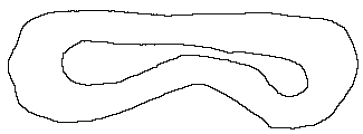
\includegraphics[interpolate=true,width=3.630000in,height=1.340000in]{contents/chapt6/figs/both/steer_velocity_lap_1-img0.png}}%
\end{pgfscope}%
\begin{pgfscope}%
\pgfpathrectangle{\pgfqpoint{0.892427in}{2.418303in}}{\pgfqpoint{3.620014in}{1.336620in}}%
\pgfusepath{clip}%
\pgfsetrectcap%
\pgfsetroundjoin%
\pgfsetlinewidth{1.505625pt}%
\definecolor{currentstroke}{rgb}{0.121569,0.466667,0.705882}%
\pgfsetstrokecolor{currentstroke}%
\pgfsetdash{}{0pt}%
\pgfpathmoveto{\pgfqpoint{3.120128in}{3.420769in}}%
\pgfpathlineto{\pgfqpoint{3.052362in}{3.421597in}}%
\pgfpathlineto{\pgfqpoint{2.997730in}{3.424568in}}%
\pgfpathlineto{\pgfqpoint{2.946530in}{3.429327in}}%
\pgfpathlineto{\pgfqpoint{2.880417in}{3.437948in}}%
\pgfpathlineto{\pgfqpoint{2.736481in}{3.457761in}}%
\pgfpathlineto{\pgfqpoint{2.680875in}{3.463295in}}%
\pgfpathlineto{\pgfqpoint{2.625102in}{3.466770in}}%
\pgfpathlineto{\pgfqpoint{2.569239in}{3.468181in}}%
\pgfpathlineto{\pgfqpoint{2.502185in}{3.467535in}}%
\pgfpathlineto{\pgfqpoint{2.323415in}{3.463581in}}%
\pgfpathlineto{\pgfqpoint{2.256388in}{3.465585in}}%
\pgfpathlineto{\pgfqpoint{2.167164in}{3.471381in}}%
\pgfpathlineto{\pgfqpoint{2.077905in}{3.476554in}}%
\pgfpathlineto{\pgfqpoint{2.022031in}{3.477331in}}%
\pgfpathlineto{\pgfqpoint{1.977348in}{3.475943in}}%
\pgfpathlineto{\pgfqpoint{1.932764in}{3.472685in}}%
\pgfpathlineto{\pgfqpoint{1.888364in}{3.467483in}}%
\pgfpathlineto{\pgfqpoint{1.844229in}{3.460372in}}%
\pgfpathlineto{\pgfqpoint{1.789494in}{3.449121in}}%
\pgfpathlineto{\pgfqpoint{1.724314in}{3.433363in}}%
\pgfpathlineto{\pgfqpoint{1.648921in}{3.412474in}}%
\pgfpathlineto{\pgfqpoint{1.595650in}{3.395598in}}%
\pgfpathlineto{\pgfqpoint{1.553592in}{3.380445in}}%
\pgfpathlineto{\pgfqpoint{1.512366in}{3.363167in}}%
\pgfpathlineto{\pgfqpoint{1.482292in}{3.348351in}}%
\pgfpathlineto{\pgfqpoint{1.453262in}{3.331585in}}%
\pgfpathlineto{\pgfqpoint{1.425633in}{3.312604in}}%
\pgfpathlineto{\pgfqpoint{1.399826in}{3.291214in}}%
\pgfpathlineto{\pgfqpoint{1.376173in}{3.267466in}}%
\pgfpathlineto{\pgfqpoint{1.361827in}{3.250328in}}%
\pgfpathlineto{\pgfqpoint{1.348779in}{3.232183in}}%
\pgfpathlineto{\pgfqpoint{1.337134in}{3.213107in}}%
\pgfpathlineto{\pgfqpoint{1.327055in}{3.193160in}}%
\pgfpathlineto{\pgfqpoint{1.318635in}{3.172457in}}%
\pgfpathlineto{\pgfqpoint{1.311967in}{3.151127in}}%
\pgfpathlineto{\pgfqpoint{1.307133in}{3.129307in}}%
\pgfpathlineto{\pgfqpoint{1.304202in}{3.107152in}}%
\pgfpathlineto{\pgfqpoint{1.303224in}{3.084825in}}%
\pgfpathlineto{\pgfqpoint{1.304125in}{3.062494in}}%
\pgfpathlineto{\pgfqpoint{1.306790in}{3.040304in}}%
\pgfpathlineto{\pgfqpoint{1.311177in}{3.018389in}}%
\pgfpathlineto{\pgfqpoint{1.317230in}{2.996875in}}%
\pgfpathlineto{\pgfqpoint{1.324868in}{2.975871in}}%
\pgfpathlineto{\pgfqpoint{1.334030in}{2.955486in}}%
\pgfpathlineto{\pgfqpoint{1.344647in}{2.935819in}}%
\pgfpathlineto{\pgfqpoint{1.356687in}{2.916989in}}%
\pgfpathlineto{\pgfqpoint{1.370087in}{2.899102in}}%
\pgfpathlineto{\pgfqpoint{1.384766in}{2.882248in}}%
\pgfpathlineto{\pgfqpoint{1.400581in}{2.866456in}}%
\pgfpathlineto{\pgfqpoint{1.417471in}{2.851819in}}%
\pgfpathlineto{\pgfqpoint{1.435355in}{2.838414in}}%
\pgfpathlineto{\pgfqpoint{1.454141in}{2.826306in}}%
\pgfpathlineto{\pgfqpoint{1.473732in}{2.815550in}}%
\pgfpathlineto{\pgfqpoint{1.494028in}{2.806191in}}%
\pgfpathlineto{\pgfqpoint{1.514926in}{2.798267in}}%
\pgfpathlineto{\pgfqpoint{1.547158in}{2.789071in}}%
\pgfpathlineto{\pgfqpoint{1.580123in}{2.782993in}}%
\pgfpathlineto{\pgfqpoint{1.613477in}{2.779624in}}%
\pgfpathlineto{\pgfqpoint{1.646987in}{2.778656in}}%
\pgfpathlineto{\pgfqpoint{1.680493in}{2.779823in}}%
\pgfpathlineto{\pgfqpoint{1.713883in}{2.782848in}}%
\pgfpathlineto{\pgfqpoint{1.758114in}{2.789310in}}%
\pgfpathlineto{\pgfqpoint{1.801942in}{2.798114in}}%
\pgfpathlineto{\pgfqpoint{1.867084in}{2.814021in}}%
\pgfpathlineto{\pgfqpoint{1.964007in}{2.840931in}}%
\pgfpathlineto{\pgfqpoint{2.071769in}{2.870561in}}%
\pgfpathlineto{\pgfqpoint{2.126314in}{2.882694in}}%
\pgfpathlineto{\pgfqpoint{2.170363in}{2.890320in}}%
\pgfpathlineto{\pgfqpoint{2.214708in}{2.895962in}}%
\pgfpathlineto{\pgfqpoint{2.270403in}{2.900518in}}%
\pgfpathlineto{\pgfqpoint{2.448757in}{2.913279in}}%
\pgfpathlineto{\pgfqpoint{2.515326in}{2.921361in}}%
\pgfpathlineto{\pgfqpoint{2.614836in}{2.936058in}}%
\pgfpathlineto{\pgfqpoint{2.703363in}{2.948600in}}%
\pgfpathlineto{\pgfqpoint{2.758953in}{2.954280in}}%
\pgfpathlineto{\pgfqpoint{2.803579in}{2.956910in}}%
\pgfpathlineto{\pgfqpoint{2.848280in}{2.957270in}}%
\pgfpathlineto{\pgfqpoint{2.892926in}{2.955060in}}%
\pgfpathlineto{\pgfqpoint{2.937342in}{2.950036in}}%
\pgfpathlineto{\pgfqpoint{2.970379in}{2.944326in}}%
\pgfpathlineto{\pgfqpoint{3.013919in}{2.934206in}}%
\pgfpathlineto{\pgfqpoint{3.056742in}{2.921387in}}%
\pgfpathlineto{\pgfqpoint{3.098789in}{2.906208in}}%
\pgfpathlineto{\pgfqpoint{3.150373in}{2.884721in}}%
\pgfpathlineto{\pgfqpoint{3.252261in}{2.838779in}}%
\pgfpathlineto{\pgfqpoint{3.415573in}{2.765924in}}%
\pgfpathlineto{\pgfqpoint{3.579059in}{2.694610in}}%
\pgfpathlineto{\pgfqpoint{3.620381in}{2.679252in}}%
\pgfpathlineto{\pgfqpoint{3.651845in}{2.669670in}}%
\pgfpathlineto{\pgfqpoint{3.683740in}{2.662268in}}%
\pgfpathlineto{\pgfqpoint{3.715994in}{2.657582in}}%
\pgfpathlineto{\pgfqpoint{3.749215in}{2.655852in}}%
\pgfpathlineto{\pgfqpoint{3.782608in}{2.656977in}}%
\pgfpathlineto{\pgfqpoint{3.815774in}{2.661017in}}%
\pgfpathlineto{\pgfqpoint{3.848455in}{2.667965in}}%
\pgfpathlineto{\pgfqpoint{3.880383in}{2.677807in}}%
\pgfpathlineto{\pgfqpoint{3.911306in}{2.690459in}}%
\pgfpathlineto{\pgfqpoint{3.940965in}{2.705843in}}%
\pgfpathlineto{\pgfqpoint{3.969184in}{2.723733in}}%
\pgfpathlineto{\pgfqpoint{3.995858in}{2.743856in}}%
\pgfpathlineto{\pgfqpoint{4.020766in}{2.766127in}}%
\pgfpathlineto{\pgfqpoint{4.043693in}{2.790431in}}%
\pgfpathlineto{\pgfqpoint{4.064473in}{2.816594in}}%
\pgfpathlineto{\pgfqpoint{4.082846in}{2.844500in}}%
\pgfpathlineto{\pgfqpoint{4.098632in}{2.873947in}}%
\pgfpathlineto{\pgfqpoint{4.111917in}{2.904605in}}%
\pgfpathlineto{\pgfqpoint{4.122536in}{2.936284in}}%
\pgfpathlineto{\pgfqpoint{4.130316in}{2.968777in}}%
\pgfpathlineto{\pgfqpoint{4.135204in}{3.001828in}}%
\pgfpathlineto{\pgfqpoint{4.136916in}{3.035193in}}%
\pgfpathlineto{\pgfqpoint{4.136258in}{3.057461in}}%
\pgfpathlineto{\pgfqpoint{4.134056in}{3.079629in}}%
\pgfpathlineto{\pgfqpoint{4.128041in}{3.112493in}}%
\pgfpathlineto{\pgfqpoint{4.118951in}{3.144641in}}%
\pgfpathlineto{\pgfqpoint{4.106755in}{3.175745in}}%
\pgfpathlineto{\pgfqpoint{4.096943in}{3.195745in}}%
\pgfpathlineto{\pgfqpoint{4.085824in}{3.215049in}}%
\pgfpathlineto{\pgfqpoint{4.073459in}{3.233580in}}%
\pgfpathlineto{\pgfqpoint{4.059846in}{3.251215in}}%
\pgfpathlineto{\pgfqpoint{4.045051in}{3.267870in}}%
\pgfpathlineto{\pgfqpoint{4.029133in}{3.283455in}}%
\pgfpathlineto{\pgfqpoint{4.003439in}{3.304810in}}%
\pgfpathlineto{\pgfqpoint{3.975919in}{3.323755in}}%
\pgfpathlineto{\pgfqpoint{3.946892in}{3.340302in}}%
\pgfpathlineto{\pgfqpoint{3.916638in}{3.354487in}}%
\pgfpathlineto{\pgfqpoint{3.885429in}{3.366426in}}%
\pgfpathlineto{\pgfqpoint{3.853521in}{3.376350in}}%
\pgfpathlineto{\pgfqpoint{3.821090in}{3.384414in}}%
\pgfpathlineto{\pgfqpoint{3.777381in}{3.393065in}}%
\pgfpathlineto{\pgfqpoint{3.722331in}{3.401540in}}%
\pgfpathlineto{\pgfqpoint{3.644925in}{3.410982in}}%
\pgfpathlineto{\pgfqpoint{3.545141in}{3.420737in}}%
\pgfpathlineto{\pgfqpoint{3.467346in}{3.426100in}}%
\pgfpathlineto{\pgfqpoint{3.400555in}{3.428627in}}%
\pgfpathlineto{\pgfqpoint{3.322578in}{3.429201in}}%
\pgfpathlineto{\pgfqpoint{3.222333in}{3.427398in}}%
\pgfpathlineto{\pgfqpoint{3.200059in}{3.426844in}}%
\pgfpathlineto{\pgfqpoint{3.200059in}{3.426844in}}%
\pgfusepath{stroke}%
\end{pgfscope}%
\begin{pgfscope}%
\pgfpathrectangle{\pgfqpoint{0.892427in}{2.418303in}}{\pgfqpoint{3.620014in}{1.336620in}}%
\pgfusepath{clip}%
\pgfsetrectcap%
\pgfsetroundjoin%
\pgfsetlinewidth{1.505625pt}%
\definecolor{currentstroke}{rgb}{1.000000,0.498039,0.054902}%
\pgfsetstrokecolor{currentstroke}%
\pgfsetdash{}{0pt}%
\pgfpathmoveto{\pgfqpoint{3.120128in}{3.420769in}}%
\pgfpathlineto{\pgfqpoint{3.043882in}{3.421668in}}%
\pgfpathlineto{\pgfqpoint{2.980192in}{3.424509in}}%
\pgfpathlineto{\pgfqpoint{2.911426in}{3.429937in}}%
\pgfpathlineto{\pgfqpoint{2.700744in}{3.448283in}}%
\pgfpathlineto{\pgfqpoint{2.602502in}{3.453636in}}%
\pgfpathlineto{\pgfqpoint{2.492292in}{3.457324in}}%
\pgfpathlineto{\pgfqpoint{2.403679in}{3.458009in}}%
\pgfpathlineto{\pgfqpoint{2.325997in}{3.456148in}}%
\pgfpathlineto{\pgfqpoint{2.248324in}{3.451675in}}%
\pgfpathlineto{\pgfqpoint{2.170746in}{3.445032in}}%
\pgfpathlineto{\pgfqpoint{2.093362in}{3.436073in}}%
\pgfpathlineto{\pgfqpoint{2.005254in}{3.423091in}}%
\pgfpathlineto{\pgfqpoint{1.873501in}{3.400815in}}%
\pgfpathlineto{\pgfqpoint{1.753051in}{3.378465in}}%
\pgfpathlineto{\pgfqpoint{1.687704in}{3.364496in}}%
\pgfpathlineto{\pgfqpoint{1.633757in}{3.350693in}}%
\pgfpathlineto{\pgfqpoint{1.591254in}{3.337356in}}%
\pgfpathlineto{\pgfqpoint{1.559992in}{3.325569in}}%
\pgfpathlineto{\pgfqpoint{1.529484in}{3.311949in}}%
\pgfpathlineto{\pgfqpoint{1.499988in}{3.296263in}}%
\pgfpathlineto{\pgfqpoint{1.471803in}{3.278329in}}%
\pgfpathlineto{\pgfqpoint{1.445301in}{3.257994in}}%
\pgfpathlineto{\pgfqpoint{1.420822in}{3.235266in}}%
\pgfpathlineto{\pgfqpoint{1.405807in}{3.218813in}}%
\pgfpathlineto{\pgfqpoint{1.391954in}{3.201372in}}%
\pgfpathlineto{\pgfqpoint{1.379359in}{3.183001in}}%
\pgfpathlineto{\pgfqpoint{1.368128in}{3.163768in}}%
\pgfpathlineto{\pgfqpoint{1.358384in}{3.143739in}}%
\pgfpathlineto{\pgfqpoint{1.350201in}{3.123024in}}%
\pgfpathlineto{\pgfqpoint{1.343653in}{3.101735in}}%
\pgfpathlineto{\pgfqpoint{1.338803in}{3.079997in}}%
\pgfpathlineto{\pgfqpoint{1.335705in}{3.057941in}}%
\pgfpathlineto{\pgfqpoint{1.334398in}{3.035707in}}%
\pgfpathlineto{\pgfqpoint{1.334840in}{3.013439in}}%
\pgfpathlineto{\pgfqpoint{1.337043in}{2.991276in}}%
\pgfpathlineto{\pgfqpoint{1.340995in}{2.969357in}}%
\pgfpathlineto{\pgfqpoint{1.346665in}{2.947818in}}%
\pgfpathlineto{\pgfqpoint{1.354008in}{2.926791in}}%
\pgfpathlineto{\pgfqpoint{1.362970in}{2.906401in}}%
\pgfpathlineto{\pgfqpoint{1.373488in}{2.886768in}}%
\pgfpathlineto{\pgfqpoint{1.385491in}{2.868007in}}%
\pgfpathlineto{\pgfqpoint{1.398875in}{2.850203in}}%
\pgfpathlineto{\pgfqpoint{1.413536in}{2.833435in}}%
\pgfpathlineto{\pgfqpoint{1.429340in}{2.817740in}}%
\pgfpathlineto{\pgfqpoint{1.446201in}{2.803186in}}%
\pgfpathlineto{\pgfqpoint{1.464020in}{2.789823in}}%
\pgfpathlineto{\pgfqpoint{1.482697in}{2.777686in}}%
\pgfpathlineto{\pgfqpoint{1.512102in}{2.761837in}}%
\pgfpathlineto{\pgfqpoint{1.542882in}{2.748858in}}%
\pgfpathlineto{\pgfqpoint{1.574704in}{2.738694in}}%
\pgfpathlineto{\pgfqpoint{1.607292in}{2.731344in}}%
\pgfpathlineto{\pgfqpoint{1.640362in}{2.726599in}}%
\pgfpathlineto{\pgfqpoint{1.673692in}{2.724297in}}%
\pgfpathlineto{\pgfqpoint{1.707101in}{2.724337in}}%
\pgfpathlineto{\pgfqpoint{1.740438in}{2.726559in}}%
\pgfpathlineto{\pgfqpoint{1.773572in}{2.730854in}}%
\pgfpathlineto{\pgfqpoint{1.806407in}{2.737032in}}%
\pgfpathlineto{\pgfqpoint{1.849659in}{2.747706in}}%
\pgfpathlineto{\pgfqpoint{1.913753in}{2.766623in}}%
\pgfpathlineto{\pgfqpoint{2.052246in}{2.808874in}}%
\pgfpathlineto{\pgfqpoint{2.148993in}{2.835124in}}%
\pgfpathlineto{\pgfqpoint{2.504855in}{2.927126in}}%
\pgfpathlineto{\pgfqpoint{2.570175in}{2.941243in}}%
\pgfpathlineto{\pgfqpoint{2.624996in}{2.951040in}}%
\pgfpathlineto{\pgfqpoint{2.669128in}{2.957139in}}%
\pgfpathlineto{\pgfqpoint{2.713474in}{2.961406in}}%
\pgfpathlineto{\pgfqpoint{2.757964in}{2.963710in}}%
\pgfpathlineto{\pgfqpoint{2.802514in}{2.963865in}}%
\pgfpathlineto{\pgfqpoint{2.847024in}{2.961973in}}%
\pgfpathlineto{\pgfqpoint{2.891402in}{2.958051in}}%
\pgfpathlineto{\pgfqpoint{2.935543in}{2.952034in}}%
\pgfpathlineto{\pgfqpoint{2.979336in}{2.943855in}}%
\pgfpathlineto{\pgfqpoint{3.022694in}{2.933615in}}%
\pgfpathlineto{\pgfqpoint{3.065537in}{2.921400in}}%
\pgfpathlineto{\pgfqpoint{3.107788in}{2.907271in}}%
\pgfpathlineto{\pgfqpoint{3.159765in}{2.887280in}}%
\pgfpathlineto{\pgfqpoint{3.273697in}{2.842224in}}%
\pgfpathlineto{\pgfqpoint{3.326329in}{2.824028in}}%
\pgfpathlineto{\pgfqpoint{3.390340in}{2.804829in}}%
\pgfpathlineto{\pgfqpoint{3.465699in}{2.784834in}}%
\pgfpathlineto{\pgfqpoint{3.530763in}{2.769577in}}%
\pgfpathlineto{\pgfqpoint{3.585365in}{2.758628in}}%
\pgfpathlineto{\pgfqpoint{3.640393in}{2.750087in}}%
\pgfpathlineto{\pgfqpoint{3.684717in}{2.745611in}}%
\pgfpathlineto{\pgfqpoint{3.729220in}{2.743642in}}%
\pgfpathlineto{\pgfqpoint{3.762616in}{2.744105in}}%
\pgfpathlineto{\pgfqpoint{3.795831in}{2.746449in}}%
\pgfpathlineto{\pgfqpoint{3.828732in}{2.750862in}}%
\pgfpathlineto{\pgfqpoint{3.861169in}{2.757475in}}%
\pgfpathlineto{\pgfqpoint{3.892937in}{2.766493in}}%
\pgfpathlineto{\pgfqpoint{3.923816in}{2.777992in}}%
\pgfpathlineto{\pgfqpoint{3.953578in}{2.791983in}}%
\pgfpathlineto{\pgfqpoint{3.981983in}{2.808535in}}%
\pgfpathlineto{\pgfqpoint{4.008813in}{2.827672in}}%
\pgfpathlineto{\pgfqpoint{4.033790in}{2.849269in}}%
\pgfpathlineto{\pgfqpoint{4.056642in}{2.873176in}}%
\pgfpathlineto{\pgfqpoint{4.070524in}{2.890344in}}%
\pgfpathlineto{\pgfqpoint{4.083233in}{2.908417in}}%
\pgfpathlineto{\pgfqpoint{4.094691in}{2.927326in}}%
\pgfpathlineto{\pgfqpoint{4.104822in}{2.946993in}}%
\pgfpathlineto{\pgfqpoint{4.113552in}{2.967329in}}%
\pgfpathlineto{\pgfqpoint{4.120814in}{2.988232in}}%
\pgfpathlineto{\pgfqpoint{4.126552in}{3.009602in}}%
\pgfpathlineto{\pgfqpoint{4.130719in}{3.031330in}}%
\pgfpathlineto{\pgfqpoint{4.133278in}{3.053304in}}%
\pgfpathlineto{\pgfqpoint{4.134203in}{3.075405in}}%
\pgfpathlineto{\pgfqpoint{4.133480in}{3.097513in}}%
\pgfpathlineto{\pgfqpoint{4.131105in}{3.119502in}}%
\pgfpathlineto{\pgfqpoint{4.127085in}{3.141251in}}%
\pgfpathlineto{\pgfqpoint{4.121441in}{3.162633in}}%
\pgfpathlineto{\pgfqpoint{4.114200in}{3.183533in}}%
\pgfpathlineto{\pgfqpoint{4.105427in}{3.203860in}}%
\pgfpathlineto{\pgfqpoint{4.095199in}{3.223513in}}%
\pgfpathlineto{\pgfqpoint{4.083574in}{3.242390in}}%
\pgfpathlineto{\pgfqpoint{4.070626in}{3.260402in}}%
\pgfpathlineto{\pgfqpoint{4.056435in}{3.277466in}}%
\pgfpathlineto{\pgfqpoint{4.041082in}{3.293506in}}%
\pgfpathlineto{\pgfqpoint{4.016081in}{3.315523in}}%
\pgfpathlineto{\pgfqpoint{3.989024in}{3.334986in}}%
\pgfpathlineto{\pgfqpoint{3.960206in}{3.351758in}}%
\pgfpathlineto{\pgfqpoint{3.930012in}{3.365937in}}%
\pgfpathlineto{\pgfqpoint{3.898856in}{3.377889in}}%
\pgfpathlineto{\pgfqpoint{3.867012in}{3.387890in}}%
\pgfpathlineto{\pgfqpoint{3.823811in}{3.398612in}}%
\pgfpathlineto{\pgfqpoint{3.780074in}{3.406937in}}%
\pgfpathlineto{\pgfqpoint{3.724978in}{3.414860in}}%
\pgfpathlineto{\pgfqpoint{3.647500in}{3.423357in}}%
\pgfpathlineto{\pgfqpoint{3.558716in}{3.430718in}}%
\pgfpathlineto{\pgfqpoint{3.447562in}{3.437672in}}%
\pgfpathlineto{\pgfqpoint{3.325160in}{3.442947in}}%
\pgfpathlineto{\pgfqpoint{3.124863in}{3.451646in}}%
\pgfpathlineto{\pgfqpoint{3.124863in}{3.451646in}}%
\pgfusepath{stroke}%
\end{pgfscope}%
\begin{pgfscope}%
\pgfpathrectangle{\pgfqpoint{0.892427in}{2.418303in}}{\pgfqpoint{3.620014in}{1.336620in}}%
\pgfusepath{clip}%
\pgfsetbuttcap%
\pgfsetroundjoin%
\pgfsetlinewidth{1.505625pt}%
\definecolor{currentstroke}{rgb}{1.000000,0.000000,0.000000}%
\pgfsetstrokecolor{currentstroke}%
\pgfsetdash{{1.500000pt}{2.475000pt}}{0.000000pt}%
\pgfpathmoveto{\pgfqpoint{3.112216in}{3.205271in}}%
\pgfpathlineto{\pgfqpoint{3.112216in}{3.650812in}}%
\pgfusepath{stroke}%
\end{pgfscope}%
\begin{pgfscope}%
\pgfsetbuttcap%
\pgfsetmiterjoin%
\definecolor{currentfill}{rgb}{1.000000,1.000000,1.000000}%
\pgfsetfillcolor{currentfill}%
\pgfsetlinewidth{1.003750pt}%
\definecolor{currentstroke}{rgb}{0.000000,0.000000,0.000000}%
\pgfsetstrokecolor{currentstroke}%
\pgfsetdash{}{0pt}%
\pgfpathmoveto{\pgfqpoint{1.734410in}{3.445162in}}%
\pgfpathlineto{\pgfqpoint{1.988892in}{3.445162in}}%
\pgfpathquadraticcurveto{\pgfqpoint{2.002775in}{3.445162in}}{\pgfqpoint{2.002775in}{3.459046in}}%
\pgfpathlineto{\pgfqpoint{2.002775in}{3.582330in}}%
\pgfpathquadraticcurveto{\pgfqpoint{2.002775in}{3.596213in}}{\pgfqpoint{1.988892in}{3.596213in}}%
\pgfpathlineto{\pgfqpoint{1.734410in}{3.596213in}}%
\pgfpathquadraticcurveto{\pgfqpoint{1.720527in}{3.596213in}}{\pgfqpoint{1.720527in}{3.582330in}}%
\pgfpathlineto{\pgfqpoint{1.720527in}{3.459046in}}%
\pgfpathquadraticcurveto{\pgfqpoint{1.720527in}{3.445162in}}{\pgfqpoint{1.734410in}{3.445162in}}%
\pgfpathlineto{\pgfqpoint{1.734410in}{3.445162in}}%
\pgfpathclose%
\pgfusepath{stroke,fill}%
\end{pgfscope}%
\begin{pgfscope}%
\definecolor{textcolor}{rgb}{0.000000,0.000000,0.000000}%
\pgfsetstrokecolor{textcolor}%
\pgfsetfillcolor{textcolor}%
\pgftext[x=1.734410in,y=3.485979in,left,base]{\color{textcolor}\rmfamily\fontsize{9.996000}{11.995200}\selectfont 20\%}%
\end{pgfscope}%
\begin{pgfscope}%
\pgfsetbuttcap%
\pgfsetmiterjoin%
\definecolor{currentfill}{rgb}{1.000000,1.000000,1.000000}%
\pgfsetfillcolor{currentfill}%
\pgfsetlinewidth{1.003750pt}%
\definecolor{currentstroke}{rgb}{0.000000,0.000000,0.000000}%
\pgfsetstrokecolor{currentstroke}%
\pgfsetdash{}{0pt}%
\pgfpathmoveto{\pgfqpoint{1.730164in}{2.689850in}}%
\pgfpathlineto{\pgfqpoint{1.984646in}{2.689850in}}%
\pgfpathquadraticcurveto{\pgfqpoint{1.998529in}{2.689850in}}{\pgfqpoint{1.998529in}{2.703733in}}%
\pgfpathlineto{\pgfqpoint{1.998529in}{2.827017in}}%
\pgfpathquadraticcurveto{\pgfqpoint{1.998529in}{2.840901in}}{\pgfqpoint{1.984646in}{2.840901in}}%
\pgfpathlineto{\pgfqpoint{1.730164in}{2.840901in}}%
\pgfpathquadraticcurveto{\pgfqpoint{1.716281in}{2.840901in}}{\pgfqpoint{1.716281in}{2.827017in}}%
\pgfpathlineto{\pgfqpoint{1.716281in}{2.703733in}}%
\pgfpathquadraticcurveto{\pgfqpoint{1.716281in}{2.689850in}}{\pgfqpoint{1.730164in}{2.689850in}}%
\pgfpathlineto{\pgfqpoint{1.730164in}{2.689850in}}%
\pgfpathclose%
\pgfusepath{stroke,fill}%
\end{pgfscope}%
\begin{pgfscope}%
\definecolor{textcolor}{rgb}{0.000000,0.000000,0.000000}%
\pgfsetstrokecolor{textcolor}%
\pgfsetfillcolor{textcolor}%
\pgftext[x=1.730164in,y=2.730667in,left,base]{\color{textcolor}\rmfamily\fontsize{9.996000}{11.995200}\selectfont 40\%}%
\end{pgfscope}%
\begin{pgfscope}%
\pgfsetbuttcap%
\pgfsetmiterjoin%
\definecolor{currentfill}{rgb}{1.000000,1.000000,1.000000}%
\pgfsetfillcolor{currentfill}%
\pgfsetlinewidth{1.003750pt}%
\definecolor{currentstroke}{rgb}{0.000000,0.000000,0.000000}%
\pgfsetstrokecolor{currentstroke}%
\pgfsetdash{}{0pt}%
\pgfpathmoveto{\pgfqpoint{3.048448in}{2.981363in}}%
\pgfpathlineto{\pgfqpoint{3.302930in}{2.981363in}}%
\pgfpathquadraticcurveto{\pgfqpoint{3.316813in}{2.981363in}}{\pgfqpoint{3.316813in}{2.995246in}}%
\pgfpathlineto{\pgfqpoint{3.316813in}{3.118530in}}%
\pgfpathquadraticcurveto{\pgfqpoint{3.316813in}{3.132414in}}{\pgfqpoint{3.302930in}{3.132414in}}%
\pgfpathlineto{\pgfqpoint{3.048448in}{3.132414in}}%
\pgfpathquadraticcurveto{\pgfqpoint{3.034565in}{3.132414in}}{\pgfqpoint{3.034565in}{3.118530in}}%
\pgfpathlineto{\pgfqpoint{3.034565in}{2.995246in}}%
\pgfpathquadraticcurveto{\pgfqpoint{3.034565in}{2.981363in}}{\pgfqpoint{3.048448in}{2.981363in}}%
\pgfpathlineto{\pgfqpoint{3.048448in}{2.981363in}}%
\pgfpathclose%
\pgfusepath{stroke,fill}%
\end{pgfscope}%
\begin{pgfscope}%
\definecolor{textcolor}{rgb}{0.000000,0.000000,0.000000}%
\pgfsetstrokecolor{textcolor}%
\pgfsetfillcolor{textcolor}%
\pgftext[x=3.048448in,y=3.022180in,left,base]{\color{textcolor}\rmfamily\fontsize{9.996000}{11.995200}\selectfont 60\%}%
\end{pgfscope}%
\begin{pgfscope}%
\pgfsetbuttcap%
\pgfsetmiterjoin%
\definecolor{currentfill}{rgb}{1.000000,1.000000,1.000000}%
\pgfsetfillcolor{currentfill}%
\pgfsetlinewidth{1.003750pt}%
\definecolor{currentstroke}{rgb}{0.000000,0.000000,0.000000}%
\pgfsetstrokecolor{currentstroke}%
\pgfsetdash{}{0pt}%
\pgfpathmoveto{\pgfqpoint{4.173629in}{2.883094in}}%
\pgfpathlineto{\pgfqpoint{4.428111in}{2.883094in}}%
\pgfpathquadraticcurveto{\pgfqpoint{4.441994in}{2.883094in}}{\pgfqpoint{4.441994in}{2.896978in}}%
\pgfpathlineto{\pgfqpoint{4.441994in}{3.020261in}}%
\pgfpathquadraticcurveto{\pgfqpoint{4.441994in}{3.034145in}}{\pgfqpoint{4.428111in}{3.034145in}}%
\pgfpathlineto{\pgfqpoint{4.173629in}{3.034145in}}%
\pgfpathquadraticcurveto{\pgfqpoint{4.159746in}{3.034145in}}{\pgfqpoint{4.159746in}{3.020261in}}%
\pgfpathlineto{\pgfqpoint{4.159746in}{2.896978in}}%
\pgfpathquadraticcurveto{\pgfqpoint{4.159746in}{2.883094in}}{\pgfqpoint{4.173629in}{2.883094in}}%
\pgfpathlineto{\pgfqpoint{4.173629in}{2.883094in}}%
\pgfpathclose%
\pgfusepath{stroke,fill}%
\end{pgfscope}%
\begin{pgfscope}%
\definecolor{textcolor}{rgb}{0.000000,0.000000,0.000000}%
\pgfsetstrokecolor{textcolor}%
\pgfsetfillcolor{textcolor}%
\pgftext[x=4.173629in,y=2.923911in,left,base]{\color{textcolor}\rmfamily\fontsize{9.996000}{11.995200}\selectfont 80\%}%
\end{pgfscope}%
\begin{pgfscope}%
\pgfsetbuttcap%
\pgfsetmiterjoin%
\definecolor{currentfill}{rgb}{1.000000,1.000000,1.000000}%
\pgfsetfillcolor{currentfill}%
\pgfsetlinewidth{1.003750pt}%
\definecolor{currentstroke}{rgb}{0.000000,0.000000,0.000000}%
\pgfsetstrokecolor{currentstroke}%
\pgfsetdash{}{0pt}%
\pgfpathmoveto{\pgfqpoint{2.844892in}{3.669051in}}%
\pgfpathlineto{\pgfqpoint{3.548222in}{3.669051in}}%
\pgfpathquadraticcurveto{\pgfqpoint{3.562105in}{3.669051in}}{\pgfqpoint{3.562105in}{3.682934in}}%
\pgfpathlineto{\pgfqpoint{3.562105in}{3.821768in}}%
\pgfpathquadraticcurveto{\pgfqpoint{3.562105in}{3.835651in}}{\pgfqpoint{3.548222in}{3.835651in}}%
\pgfpathlineto{\pgfqpoint{2.844892in}{3.835651in}}%
\pgfpathquadraticcurveto{\pgfqpoint{2.831008in}{3.835651in}}{\pgfqpoint{2.831008in}{3.821768in}}%
\pgfpathlineto{\pgfqpoint{2.831008in}{3.682934in}}%
\pgfpathquadraticcurveto{\pgfqpoint{2.831008in}{3.669051in}}{\pgfqpoint{2.844892in}{3.669051in}}%
\pgfpathlineto{\pgfqpoint{2.844892in}{3.669051in}}%
\pgfpathclose%
\pgfusepath{stroke,fill}%
\end{pgfscope}%
\begin{pgfscope}%
\definecolor{textcolor}{rgb}{0.000000,0.000000,0.000000}%
\pgfsetstrokecolor{textcolor}%
\pgfsetfillcolor{textcolor}%
\pgftext[x=2.844892in,y=3.717643in,left,base]{\color{textcolor}\rmfamily\fontsize{9.996000}{11.995200}\selectfont Start/finish}%
\end{pgfscope}%
\begin{pgfscope}%
\pgfsetbuttcap%
\pgfsetmiterjoin%
\definecolor{currentfill}{rgb}{1.000000,1.000000,1.000000}%
\pgfsetfillcolor{currentfill}%
\pgfsetlinewidth{0.000000pt}%
\definecolor{currentstroke}{rgb}{0.000000,0.000000,0.000000}%
\pgfsetstrokecolor{currentstroke}%
\pgfsetstrokeopacity{0.000000}%
\pgfsetdash{}{0pt}%
\pgfpathmoveto{\pgfqpoint{0.707263in}{0.920000in}}%
\pgfpathlineto{\pgfqpoint{4.697605in}{0.920000in}}%
\pgfpathlineto{\pgfqpoint{4.697605in}{2.256620in}}%
\pgfpathlineto{\pgfqpoint{0.707263in}{2.256620in}}%
\pgfpathlineto{\pgfqpoint{0.707263in}{0.920000in}}%
\pgfpathclose%
\pgfusepath{fill}%
\end{pgfscope}%
\begin{pgfscope}%
\pgfpathrectangle{\pgfqpoint{0.707263in}{0.920000in}}{\pgfqpoint{3.990343in}{1.336620in}}%
\pgfusepath{clip}%
\pgfsetrectcap%
\pgfsetroundjoin%
\pgfsetlinewidth{0.803000pt}%
\definecolor{currentstroke}{rgb}{0.827451,0.827451,0.827451}%
\pgfsetstrokecolor{currentstroke}%
\pgfsetdash{}{0pt}%
\pgfpathmoveto{\pgfqpoint{0.707263in}{0.920000in}}%
\pgfpathlineto{\pgfqpoint{0.707263in}{2.256620in}}%
\pgfusepath{stroke}%
\end{pgfscope}%
\begin{pgfscope}%
\definecolor{textcolor}{rgb}{0.000000,0.000000,0.000000}%
\pgfsetstrokecolor{textcolor}%
\pgfsetfillcolor{textcolor}%
\pgftext[x=0.707263in,y=0.871389in,,top]{\color{textcolor}\rmfamily\fontsize{12.000000}{14.400000}\selectfont \(\displaystyle {0}\)}%
\end{pgfscope}%
\begin{pgfscope}%
\pgfpathrectangle{\pgfqpoint{0.707263in}{0.920000in}}{\pgfqpoint{3.990343in}{1.336620in}}%
\pgfusepath{clip}%
\pgfsetrectcap%
\pgfsetroundjoin%
\pgfsetlinewidth{0.803000pt}%
\definecolor{currentstroke}{rgb}{0.827451,0.827451,0.827451}%
\pgfsetstrokecolor{currentstroke}%
\pgfsetdash{}{0pt}%
\pgfpathmoveto{\pgfqpoint{1.505331in}{0.920000in}}%
\pgfpathlineto{\pgfqpoint{1.505331in}{2.256620in}}%
\pgfusepath{stroke}%
\end{pgfscope}%
\begin{pgfscope}%
\definecolor{textcolor}{rgb}{0.000000,0.000000,0.000000}%
\pgfsetstrokecolor{textcolor}%
\pgfsetfillcolor{textcolor}%
\pgftext[x=1.505331in,y=0.871389in,,top]{\color{textcolor}\rmfamily\fontsize{12.000000}{14.400000}\selectfont \(\displaystyle {20}\)}%
\end{pgfscope}%
\begin{pgfscope}%
\pgfpathrectangle{\pgfqpoint{0.707263in}{0.920000in}}{\pgfqpoint{3.990343in}{1.336620in}}%
\pgfusepath{clip}%
\pgfsetrectcap%
\pgfsetroundjoin%
\pgfsetlinewidth{0.803000pt}%
\definecolor{currentstroke}{rgb}{0.827451,0.827451,0.827451}%
\pgfsetstrokecolor{currentstroke}%
\pgfsetdash{}{0pt}%
\pgfpathmoveto{\pgfqpoint{2.303400in}{0.920000in}}%
\pgfpathlineto{\pgfqpoint{2.303400in}{2.256620in}}%
\pgfusepath{stroke}%
\end{pgfscope}%
\begin{pgfscope}%
\definecolor{textcolor}{rgb}{0.000000,0.000000,0.000000}%
\pgfsetstrokecolor{textcolor}%
\pgfsetfillcolor{textcolor}%
\pgftext[x=2.303400in,y=0.871389in,,top]{\color{textcolor}\rmfamily\fontsize{12.000000}{14.400000}\selectfont \(\displaystyle {40}\)}%
\end{pgfscope}%
\begin{pgfscope}%
\pgfpathrectangle{\pgfqpoint{0.707263in}{0.920000in}}{\pgfqpoint{3.990343in}{1.336620in}}%
\pgfusepath{clip}%
\pgfsetrectcap%
\pgfsetroundjoin%
\pgfsetlinewidth{0.803000pt}%
\definecolor{currentstroke}{rgb}{0.827451,0.827451,0.827451}%
\pgfsetstrokecolor{currentstroke}%
\pgfsetdash{}{0pt}%
\pgfpathmoveto{\pgfqpoint{3.101468in}{0.920000in}}%
\pgfpathlineto{\pgfqpoint{3.101468in}{2.256620in}}%
\pgfusepath{stroke}%
\end{pgfscope}%
\begin{pgfscope}%
\definecolor{textcolor}{rgb}{0.000000,0.000000,0.000000}%
\pgfsetstrokecolor{textcolor}%
\pgfsetfillcolor{textcolor}%
\pgftext[x=3.101468in,y=0.871389in,,top]{\color{textcolor}\rmfamily\fontsize{12.000000}{14.400000}\selectfont \(\displaystyle {60}\)}%
\end{pgfscope}%
\begin{pgfscope}%
\pgfpathrectangle{\pgfqpoint{0.707263in}{0.920000in}}{\pgfqpoint{3.990343in}{1.336620in}}%
\pgfusepath{clip}%
\pgfsetrectcap%
\pgfsetroundjoin%
\pgfsetlinewidth{0.803000pt}%
\definecolor{currentstroke}{rgb}{0.827451,0.827451,0.827451}%
\pgfsetstrokecolor{currentstroke}%
\pgfsetdash{}{0pt}%
\pgfpathmoveto{\pgfqpoint{3.899537in}{0.920000in}}%
\pgfpathlineto{\pgfqpoint{3.899537in}{2.256620in}}%
\pgfusepath{stroke}%
\end{pgfscope}%
\begin{pgfscope}%
\definecolor{textcolor}{rgb}{0.000000,0.000000,0.000000}%
\pgfsetstrokecolor{textcolor}%
\pgfsetfillcolor{textcolor}%
\pgftext[x=3.899537in,y=0.871389in,,top]{\color{textcolor}\rmfamily\fontsize{12.000000}{14.400000}\selectfont \(\displaystyle {80}\)}%
\end{pgfscope}%
\begin{pgfscope}%
\pgfpathrectangle{\pgfqpoint{0.707263in}{0.920000in}}{\pgfqpoint{3.990343in}{1.336620in}}%
\pgfusepath{clip}%
\pgfsetrectcap%
\pgfsetroundjoin%
\pgfsetlinewidth{0.803000pt}%
\definecolor{currentstroke}{rgb}{0.827451,0.827451,0.827451}%
\pgfsetstrokecolor{currentstroke}%
\pgfsetdash{}{0pt}%
\pgfpathmoveto{\pgfqpoint{4.697605in}{0.920000in}}%
\pgfpathlineto{\pgfqpoint{4.697605in}{2.256620in}}%
\pgfusepath{stroke}%
\end{pgfscope}%
\begin{pgfscope}%
\definecolor{textcolor}{rgb}{0.000000,0.000000,0.000000}%
\pgfsetstrokecolor{textcolor}%
\pgfsetfillcolor{textcolor}%
\pgftext[x=4.697605in,y=0.871389in,,top]{\color{textcolor}\rmfamily\fontsize{12.000000}{14.400000}\selectfont \(\displaystyle {100}\)}%
\end{pgfscope}%
\begin{pgfscope}%
\definecolor{textcolor}{rgb}{0.000000,0.000000,0.000000}%
\pgfsetstrokecolor{textcolor}%
\pgfsetfillcolor{textcolor}%
\pgftext[x=2.702434in,y=0.667833in,,top]{\color{textcolor}\rmfamily\fontsize{12.000000}{14.400000}\selectfont Progress along centerline [\%]}%
\end{pgfscope}%
\begin{pgfscope}%
\pgfpathrectangle{\pgfqpoint{0.707263in}{0.920000in}}{\pgfqpoint{3.990343in}{1.336620in}}%
\pgfusepath{clip}%
\pgfsetrectcap%
\pgfsetroundjoin%
\pgfsetlinewidth{0.803000pt}%
\definecolor{currentstroke}{rgb}{0.827451,0.827451,0.827451}%
\pgfsetstrokecolor{currentstroke}%
\pgfsetdash{}{0pt}%
\pgfpathmoveto{\pgfqpoint{0.707263in}{1.031385in}}%
\pgfpathlineto{\pgfqpoint{4.697605in}{1.031385in}}%
\pgfusepath{stroke}%
\end{pgfscope}%
\begin{pgfscope}%
\definecolor{textcolor}{rgb}{0.000000,0.000000,0.000000}%
\pgfsetstrokecolor{textcolor}%
\pgfsetfillcolor{textcolor}%
\pgftext[x=0.577055in, y=0.973552in, left, base]{\color{textcolor}\rmfamily\fontsize{12.000000}{14.400000}\selectfont \(\displaystyle {3}\)}%
\end{pgfscope}%
\begin{pgfscope}%
\pgfpathrectangle{\pgfqpoint{0.707263in}{0.920000in}}{\pgfqpoint{3.990343in}{1.336620in}}%
\pgfusepath{clip}%
\pgfsetrectcap%
\pgfsetroundjoin%
\pgfsetlinewidth{0.803000pt}%
\definecolor{currentstroke}{rgb}{0.827451,0.827451,0.827451}%
\pgfsetstrokecolor{currentstroke}%
\pgfsetdash{}{0pt}%
\pgfpathmoveto{\pgfqpoint{0.707263in}{1.588310in}}%
\pgfpathlineto{\pgfqpoint{4.697605in}{1.588310in}}%
\pgfusepath{stroke}%
\end{pgfscope}%
\begin{pgfscope}%
\definecolor{textcolor}{rgb}{0.000000,0.000000,0.000000}%
\pgfsetstrokecolor{textcolor}%
\pgfsetfillcolor{textcolor}%
\pgftext[x=0.577055in, y=1.530477in, left, base]{\color{textcolor}\rmfamily\fontsize{12.000000}{14.400000}\selectfont \(\displaystyle {4}\)}%
\end{pgfscope}%
\begin{pgfscope}%
\pgfpathrectangle{\pgfqpoint{0.707263in}{0.920000in}}{\pgfqpoint{3.990343in}{1.336620in}}%
\pgfusepath{clip}%
\pgfsetrectcap%
\pgfsetroundjoin%
\pgfsetlinewidth{0.803000pt}%
\definecolor{currentstroke}{rgb}{0.827451,0.827451,0.827451}%
\pgfsetstrokecolor{currentstroke}%
\pgfsetdash{}{0pt}%
\pgfpathmoveto{\pgfqpoint{0.707263in}{2.145235in}}%
\pgfpathlineto{\pgfqpoint{4.697605in}{2.145235in}}%
\pgfusepath{stroke}%
\end{pgfscope}%
\begin{pgfscope}%
\definecolor{textcolor}{rgb}{0.000000,0.000000,0.000000}%
\pgfsetstrokecolor{textcolor}%
\pgfsetfillcolor{textcolor}%
\pgftext[x=0.577055in, y=2.087402in, left, base]{\color{textcolor}\rmfamily\fontsize{12.000000}{14.400000}\selectfont \(\displaystyle {5}\)}%
\end{pgfscope}%
\begin{pgfscope}%
\definecolor{textcolor}{rgb}{0.000000,0.000000,0.000000}%
\pgfsetstrokecolor{textcolor}%
\pgfsetfillcolor{textcolor}%
\pgftext[x=0.295667in, y=1.133727in, left, base,rotate=90.000000]{\color{textcolor}\rmfamily\fontsize{12.000000}{14.400000}\selectfont Longitudinal}%
\end{pgfscope}%
\begin{pgfscope}%
\definecolor{textcolor}{rgb}{0.000000,0.000000,0.000000}%
\pgfsetstrokecolor{textcolor}%
\pgfsetfillcolor{textcolor}%
\pgftext[x=0.479833in, y=1.100477in, left, base,rotate=90.000000]{\color{textcolor}\rmfamily\fontsize{12.000000}{14.400000}\selectfont velocity [m/s]}%
\end{pgfscope}%
\begin{pgfscope}%
\pgfpathrectangle{\pgfqpoint{0.707263in}{0.920000in}}{\pgfqpoint{3.990343in}{1.336620in}}%
\pgfusepath{clip}%
\pgfsetbuttcap%
\pgfsetroundjoin%
\pgfsetlinewidth{1.505625pt}%
\definecolor{currentstroke}{rgb}{0.000000,0.000000,0.000000}%
\pgfsetstrokecolor{currentstroke}%
\pgfsetdash{{5.550000pt}{2.400000pt}}{0.000000pt}%
\pgfpathmoveto{\pgfqpoint{0.707263in}{1.031385in}}%
\pgfpathlineto{\pgfqpoint{4.697605in}{1.031385in}}%
\pgfusepath{stroke}%
\end{pgfscope}%
\begin{pgfscope}%
\pgfpathrectangle{\pgfqpoint{0.707263in}{0.920000in}}{\pgfqpoint{3.990343in}{1.336620in}}%
\pgfusepath{clip}%
\pgfsetbuttcap%
\pgfsetroundjoin%
\pgfsetlinewidth{1.505625pt}%
\definecolor{currentstroke}{rgb}{0.000000,0.000000,0.000000}%
\pgfsetstrokecolor{currentstroke}%
\pgfsetdash{{5.550000pt}{2.400000pt}}{0.000000pt}%
\pgfpathmoveto{\pgfqpoint{0.707263in}{2.145235in}}%
\pgfpathlineto{\pgfqpoint{4.697605in}{2.145235in}}%
\pgfusepath{stroke}%
\end{pgfscope}%
\begin{pgfscope}%
\pgfpathrectangle{\pgfqpoint{0.707263in}{0.920000in}}{\pgfqpoint{3.990343in}{1.336620in}}%
\pgfusepath{clip}%
\pgfsetrectcap%
\pgfsetroundjoin%
\pgfsetlinewidth{1.505625pt}%
\definecolor{currentstroke}{rgb}{0.121569,0.466667,0.705882}%
\pgfsetstrokecolor{currentstroke}%
\pgfsetdash{}{0pt}%
\pgfpathmoveto{\pgfqpoint{0.707263in}{1.031385in}}%
\pgfpathlineto{\pgfqpoint{0.707263in}{1.137312in}}%
\pgfpathlineto{\pgfqpoint{0.720218in}{1.190276in}}%
\pgfpathlineto{\pgfqpoint{0.720218in}{1.296203in}}%
\pgfpathlineto{\pgfqpoint{0.733174in}{1.349167in}}%
\pgfpathlineto{\pgfqpoint{0.733174in}{1.455094in}}%
\pgfpathlineto{\pgfqpoint{0.746130in}{1.508057in}}%
\pgfpathlineto{\pgfqpoint{0.746130in}{1.613984in}}%
\pgfpathlineto{\pgfqpoint{0.759085in}{1.666948in}}%
\pgfpathlineto{\pgfqpoint{0.759085in}{1.719912in}}%
\pgfpathlineto{\pgfqpoint{0.772041in}{1.772875in}}%
\pgfpathlineto{\pgfqpoint{0.772041in}{1.825839in}}%
\pgfpathlineto{\pgfqpoint{0.784997in}{1.878802in}}%
\pgfpathlineto{\pgfqpoint{0.784997in}{1.984730in}}%
\pgfpathlineto{\pgfqpoint{0.797952in}{2.037693in}}%
\pgfpathlineto{\pgfqpoint{0.797952in}{2.090657in}}%
\pgfpathlineto{\pgfqpoint{0.810908in}{2.122728in}}%
\pgfpathlineto{\pgfqpoint{0.810908in}{2.154798in}}%
\pgfpathlineto{\pgfqpoint{3.427951in}{2.154798in}}%
\pgfpathlineto{\pgfqpoint{3.427951in}{2.150729in}}%
\pgfpathlineto{\pgfqpoint{3.440907in}{2.146659in}}%
\pgfpathlineto{\pgfqpoint{3.440907in}{2.138519in}}%
\pgfpathlineto{\pgfqpoint{3.453862in}{2.134450in}}%
\pgfpathlineto{\pgfqpoint{3.453862in}{2.130380in}}%
\pgfpathlineto{\pgfqpoint{3.466818in}{2.126310in}}%
\pgfpathlineto{\pgfqpoint{3.466818in}{2.122240in}}%
\pgfpathlineto{\pgfqpoint{3.479774in}{2.118171in}}%
\pgfpathlineto{\pgfqpoint{3.479774in}{2.114101in}}%
\pgfpathlineto{\pgfqpoint{3.492729in}{2.110031in}}%
\pgfpathlineto{\pgfqpoint{3.492729in}{2.105961in}}%
\pgfpathlineto{\pgfqpoint{3.505685in}{2.101892in}}%
\pgfpathlineto{\pgfqpoint{3.505685in}{2.097822in}}%
\pgfpathlineto{\pgfqpoint{3.518641in}{2.093752in}}%
\pgfpathlineto{\pgfqpoint{3.518641in}{2.089682in}}%
\pgfpathlineto{\pgfqpoint{3.531596in}{2.085613in}}%
\pgfpathlineto{\pgfqpoint{3.531596in}{2.081543in}}%
\pgfpathlineto{\pgfqpoint{3.544552in}{2.077473in}}%
\pgfpathlineto{\pgfqpoint{3.544552in}{2.073404in}}%
\pgfpathlineto{\pgfqpoint{3.557507in}{2.109543in}}%
\pgfpathlineto{\pgfqpoint{3.557507in}{2.145682in}}%
\pgfpathlineto{\pgfqpoint{4.645783in}{2.145682in}}%
\pgfpathlineto{\pgfqpoint{4.645783in}{2.145682in}}%
\pgfusepath{stroke}%
\end{pgfscope}%
\begin{pgfscope}%
\pgfpathrectangle{\pgfqpoint{0.707263in}{0.920000in}}{\pgfqpoint{3.990343in}{1.336620in}}%
\pgfusepath{clip}%
\pgfsetrectcap%
\pgfsetroundjoin%
\pgfsetlinewidth{1.505625pt}%
\definecolor{currentstroke}{rgb}{1.000000,0.498039,0.054902}%
\pgfsetstrokecolor{currentstroke}%
\pgfsetdash{}{0pt}%
\pgfpathmoveto{\pgfqpoint{0.707263in}{1.031385in}}%
\pgfpathlineto{\pgfqpoint{0.707263in}{1.137312in}}%
\pgfpathlineto{\pgfqpoint{0.720218in}{1.190276in}}%
\pgfpathlineto{\pgfqpoint{0.720218in}{1.296203in}}%
\pgfpathlineto{\pgfqpoint{0.733174in}{1.349167in}}%
\pgfpathlineto{\pgfqpoint{0.733174in}{1.446908in}}%
\pgfpathlineto{\pgfqpoint{0.746130in}{1.491182in}}%
\pgfpathlineto{\pgfqpoint{0.746130in}{1.571487in}}%
\pgfpathlineto{\pgfqpoint{0.759085in}{1.607863in}}%
\pgfpathlineto{\pgfqpoint{0.759085in}{1.641932in}}%
\pgfpathlineto{\pgfqpoint{0.772041in}{1.673842in}}%
\pgfpathlineto{\pgfqpoint{0.772041in}{1.731720in}}%
\pgfpathlineto{\pgfqpoint{0.784997in}{1.757936in}}%
\pgfpathlineto{\pgfqpoint{0.784997in}{1.782491in}}%
\pgfpathlineto{\pgfqpoint{0.797952in}{1.805489in}}%
\pgfpathlineto{\pgfqpoint{0.797952in}{1.827029in}}%
\pgfpathlineto{\pgfqpoint{0.810908in}{1.847203in}}%
\pgfpathlineto{\pgfqpoint{0.810908in}{1.866099in}}%
\pgfpathlineto{\pgfqpoint{0.823864in}{1.883796in}}%
\pgfpathlineto{\pgfqpoint{0.823864in}{1.915896in}}%
\pgfpathlineto{\pgfqpoint{0.836819in}{1.930436in}}%
\pgfpathlineto{\pgfqpoint{0.836819in}{1.944054in}}%
\pgfpathlineto{\pgfqpoint{0.849775in}{1.956809in}}%
\pgfpathlineto{\pgfqpoint{0.849775in}{1.968755in}}%
\pgfpathlineto{\pgfqpoint{0.862731in}{1.979944in}}%
\pgfpathlineto{\pgfqpoint{0.862731in}{1.990423in}}%
\pgfpathlineto{\pgfqpoint{0.875686in}{2.000239in}}%
\pgfpathlineto{\pgfqpoint{0.875686in}{2.009431in}}%
\pgfpathlineto{\pgfqpoint{0.888642in}{2.018041in}}%
\pgfpathlineto{\pgfqpoint{0.888642in}{2.026105in}}%
\pgfpathlineto{\pgfqpoint{0.901598in}{2.033658in}}%
\pgfpathlineto{\pgfqpoint{0.901598in}{2.040732in}}%
\pgfpathlineto{\pgfqpoint{0.914553in}{2.047358in}}%
\pgfpathlineto{\pgfqpoint{0.914553in}{2.053563in}}%
\pgfpathlineto{\pgfqpoint{0.927509in}{2.059375in}}%
\pgfpathlineto{\pgfqpoint{0.927509in}{2.064819in}}%
\pgfpathlineto{\pgfqpoint{0.940464in}{2.069917in}}%
\pgfpathlineto{\pgfqpoint{0.940464in}{2.074692in}}%
\pgfpathlineto{\pgfqpoint{0.953420in}{2.079165in}}%
\pgfpathlineto{\pgfqpoint{0.953420in}{2.083354in}}%
\pgfpathlineto{\pgfqpoint{0.966376in}{2.087277in}}%
\pgfpathlineto{\pgfqpoint{0.966376in}{2.090952in}}%
\pgfpathlineto{\pgfqpoint{0.979331in}{2.094393in}}%
\pgfpathlineto{\pgfqpoint{0.979331in}{2.100636in}}%
\pgfpathlineto{\pgfqpoint{0.992287in}{2.103463in}}%
\pgfpathlineto{\pgfqpoint{0.992287in}{2.106112in}}%
\pgfpathlineto{\pgfqpoint{1.005243in}{2.108592in}}%
\pgfpathlineto{\pgfqpoint{1.005243in}{2.110915in}}%
\pgfpathlineto{\pgfqpoint{1.018198in}{2.113091in}}%
\pgfpathlineto{\pgfqpoint{1.018198in}{2.115129in}}%
\pgfpathlineto{\pgfqpoint{1.031154in}{2.117038in}}%
\pgfpathlineto{\pgfqpoint{1.031154in}{2.118826in}}%
\pgfpathlineto{\pgfqpoint{1.044110in}{2.120500in}}%
\pgfpathlineto{\pgfqpoint{1.044110in}{2.122068in}}%
\pgfpathlineto{\pgfqpoint{1.057065in}{2.123537in}}%
\pgfpathlineto{\pgfqpoint{1.057065in}{2.124913in}}%
\pgfpathlineto{\pgfqpoint{1.070021in}{2.126201in}}%
\pgfpathlineto{\pgfqpoint{1.070021in}{2.127408in}}%
\pgfpathlineto{\pgfqpoint{1.095932in}{2.130588in}}%
\pgfpathlineto{\pgfqpoint{1.095932in}{2.131517in}}%
\pgfpathlineto{\pgfqpoint{1.121844in}{2.133964in}}%
\pgfpathlineto{\pgfqpoint{1.121844in}{2.134679in}}%
\pgfpathlineto{\pgfqpoint{1.160711in}{2.137627in}}%
\pgfpathlineto{\pgfqpoint{1.160711in}{2.138109in}}%
\pgfpathlineto{\pgfqpoint{1.225489in}{2.141283in}}%
\pgfpathlineto{\pgfqpoint{1.225489in}{2.141534in}}%
\pgfpathlineto{\pgfqpoint{1.471646in}{2.144926in}}%
\pgfpathlineto{\pgfqpoint{2.404454in}{2.145235in}}%
\pgfpathlineto{\pgfqpoint{3.570463in}{2.145230in}}%
\pgfpathlineto{\pgfqpoint{3.583419in}{2.141947in}}%
\pgfpathlineto{\pgfqpoint{3.583419in}{2.138790in}}%
\pgfpathlineto{\pgfqpoint{3.609330in}{2.132830in}}%
\pgfpathlineto{\pgfqpoint{3.609330in}{2.130019in}}%
\pgfpathlineto{\pgfqpoint{3.635241in}{2.124714in}}%
\pgfpathlineto{\pgfqpoint{3.635241in}{2.122212in}}%
\pgfpathlineto{\pgfqpoint{3.648197in}{2.119805in}}%
\pgfpathlineto{\pgfqpoint{3.648197in}{2.117490in}}%
\pgfpathlineto{\pgfqpoint{3.674108in}{2.113120in}}%
\pgfpathlineto{\pgfqpoint{3.674108in}{2.111059in}}%
\pgfpathlineto{\pgfqpoint{3.687064in}{2.109076in}}%
\pgfpathlineto{\pgfqpoint{3.687064in}{2.107169in}}%
\pgfpathlineto{\pgfqpoint{3.712975in}{2.103570in}}%
\pgfpathlineto{\pgfqpoint{3.712975in}{2.101872in}}%
\pgfpathlineto{\pgfqpoint{3.725931in}{2.100239in}}%
\pgfpathlineto{\pgfqpoint{3.725931in}{2.098668in}}%
\pgfpathlineto{\pgfqpoint{3.751842in}{2.103516in}}%
\pgfpathlineto{\pgfqpoint{3.751842in}{2.105713in}}%
\pgfpathlineto{\pgfqpoint{3.777754in}{2.109696in}}%
\pgfpathlineto{\pgfqpoint{3.777754in}{2.111501in}}%
\pgfpathlineto{\pgfqpoint{3.803665in}{2.114774in}}%
\pgfpathlineto{\pgfqpoint{3.803665in}{2.116256in}}%
\pgfpathlineto{\pgfqpoint{3.829576in}{2.118945in}}%
\pgfpathlineto{\pgfqpoint{3.829576in}{2.120163in}}%
\pgfpathlineto{\pgfqpoint{3.868443in}{2.124311in}}%
\pgfpathlineto{\pgfqpoint{3.868443in}{2.125189in}}%
\pgfpathlineto{\pgfqpoint{3.907310in}{2.127354in}}%
\pgfpathlineto{\pgfqpoint{3.907310in}{2.127211in}}%
\pgfpathlineto{\pgfqpoint{4.049822in}{2.125400in}}%
\pgfpathlineto{\pgfqpoint{4.049822in}{2.126654in}}%
\pgfpathlineto{\pgfqpoint{4.075734in}{2.129959in}}%
\pgfpathlineto{\pgfqpoint{4.075734in}{2.130924in}}%
\pgfpathlineto{\pgfqpoint{4.114601in}{2.134210in}}%
\pgfpathlineto{\pgfqpoint{4.114601in}{2.134906in}}%
\pgfpathlineto{\pgfqpoint{4.153468in}{2.137776in}}%
\pgfpathlineto{\pgfqpoint{4.153468in}{2.138245in}}%
\pgfpathlineto{\pgfqpoint{4.218246in}{2.141349in}}%
\pgfpathlineto{\pgfqpoint{4.218246in}{2.141596in}}%
\pgfpathlineto{\pgfqpoint{4.464404in}{2.144952in}}%
\pgfpathlineto{\pgfqpoint{4.697605in}{2.145205in}}%
\pgfpathlineto{\pgfqpoint{4.697605in}{2.145205in}}%
\pgfusepath{stroke}%
\end{pgfscope}%
\begin{pgfscope}%
\pgfsetrectcap%
\pgfsetmiterjoin%
\pgfsetlinewidth{0.803000pt}%
\definecolor{currentstroke}{rgb}{0.501961,0.501961,0.501961}%
\pgfsetstrokecolor{currentstroke}%
\pgfsetdash{}{0pt}%
\pgfpathmoveto{\pgfqpoint{0.707263in}{0.920000in}}%
\pgfpathlineto{\pgfqpoint{0.707263in}{2.256620in}}%
\pgfusepath{stroke}%
\end{pgfscope}%
\begin{pgfscope}%
\pgfsetrectcap%
\pgfsetmiterjoin%
\pgfsetlinewidth{0.803000pt}%
\definecolor{currentstroke}{rgb}{0.501961,0.501961,0.501961}%
\pgfsetstrokecolor{currentstroke}%
\pgfsetdash{}{0pt}%
\pgfpathmoveto{\pgfqpoint{4.697605in}{0.920000in}}%
\pgfpathlineto{\pgfqpoint{4.697605in}{2.256620in}}%
\pgfusepath{stroke}%
\end{pgfscope}%
\begin{pgfscope}%
\pgfsetrectcap%
\pgfsetmiterjoin%
\pgfsetlinewidth{0.803000pt}%
\definecolor{currentstroke}{rgb}{0.501961,0.501961,0.501961}%
\pgfsetstrokecolor{currentstroke}%
\pgfsetdash{}{0pt}%
\pgfpathmoveto{\pgfqpoint{0.707263in}{0.920000in}}%
\pgfpathlineto{\pgfqpoint{4.697605in}{0.920000in}}%
\pgfusepath{stroke}%
\end{pgfscope}%
\begin{pgfscope}%
\pgfsetrectcap%
\pgfsetmiterjoin%
\pgfsetlinewidth{0.803000pt}%
\definecolor{currentstroke}{rgb}{0.501961,0.501961,0.501961}%
\pgfsetstrokecolor{currentstroke}%
\pgfsetdash{}{0pt}%
\pgfpathmoveto{\pgfqpoint{0.707263in}{2.256620in}}%
\pgfpathlineto{\pgfqpoint{4.697605in}{2.256620in}}%
\pgfusepath{stroke}%
\end{pgfscope}%
\begin{pgfscope}%
\pgfsetbuttcap%
\pgfsetmiterjoin%
\definecolor{currentfill}{rgb}{1.000000,1.000000,1.000000}%
\pgfsetfillcolor{currentfill}%
\pgfsetfillopacity{0.800000}%
\pgfsetlinewidth{1.003750pt}%
\definecolor{currentstroke}{rgb}{0.800000,0.800000,0.800000}%
\pgfsetstrokecolor{currentstroke}%
\pgfsetstrokeopacity{0.800000}%
\pgfsetdash{}{0pt}%
\pgfpathmoveto{\pgfqpoint{0.244167in}{0.083333in}}%
\pgfpathlineto{\pgfqpoint{4.755833in}{0.083333in}}%
\pgfpathquadraticcurveto{\pgfqpoint{4.789167in}{0.083333in}}{\pgfqpoint{4.789167in}{0.116667in}}%
\pgfpathlineto{\pgfqpoint{4.789167in}{0.334833in}}%
\pgfpathquadraticcurveto{\pgfqpoint{4.789167in}{0.368167in}}{\pgfqpoint{4.755833in}{0.368167in}}%
\pgfpathlineto{\pgfqpoint{0.244167in}{0.368167in}}%
\pgfpathquadraticcurveto{\pgfqpoint{0.210833in}{0.368167in}}{\pgfqpoint{0.210833in}{0.334833in}}%
\pgfpathlineto{\pgfqpoint{0.210833in}{0.116667in}}%
\pgfpathquadraticcurveto{\pgfqpoint{0.210833in}{0.083333in}}{\pgfqpoint{0.244167in}{0.083333in}}%
\pgfpathlineto{\pgfqpoint{0.244167in}{0.083333in}}%
\pgfpathclose%
\pgfusepath{stroke,fill}%
\end{pgfscope}%
\begin{pgfscope}%
\pgfsetrectcap%
\pgfsetroundjoin%
\pgfsetlinewidth{1.505625pt}%
\definecolor{currentstroke}{rgb}{0.121569,0.466667,0.705882}%
\pgfsetstrokecolor{currentstroke}%
\pgfsetdash{}{0pt}%
\pgfpathmoveto{\pgfqpoint{0.277500in}{0.242500in}}%
\pgfpathlineto{\pgfqpoint{0.444167in}{0.242500in}}%
\pgfpathlineto{\pgfqpoint{0.610833in}{0.242500in}}%
\pgfusepath{stroke}%
\end{pgfscope}%
\begin{pgfscope}%
\definecolor{textcolor}{rgb}{0.000000,0.000000,0.000000}%
\pgfsetstrokecolor{textcolor}%
\pgfsetfillcolor{textcolor}%
\pgftext[x=0.744167in,y=0.184167in,left,base]{\color{textcolor}\rmfamily\fontsize{12.000000}{14.400000}\selectfont Steering control}%
\end{pgfscope}%
\begin{pgfscope}%
\pgfsetrectcap%
\pgfsetroundjoin%
\pgfsetlinewidth{1.505625pt}%
\definecolor{currentstroke}{rgb}{1.000000,0.498039,0.054902}%
\pgfsetstrokecolor{currentstroke}%
\pgfsetdash{}{0pt}%
\pgfpathmoveto{\pgfqpoint{2.206500in}{0.242500in}}%
\pgfpathlineto{\pgfqpoint{2.373167in}{0.242500in}}%
\pgfpathlineto{\pgfqpoint{2.539833in}{0.242500in}}%
\pgfusepath{stroke}%
\end{pgfscope}%
\begin{pgfscope}%
\definecolor{textcolor}{rgb}{0.000000,0.000000,0.000000}%
\pgfsetstrokecolor{textcolor}%
\pgfsetfillcolor{textcolor}%
\pgftext[x=2.673167in,y=0.184167in,left,base]{\color{textcolor}\rmfamily\fontsize{12.000000}{14.400000}\selectfont Steering and velocity control}%
\end{pgfscope}%
\end{pgfpicture}%
\makeatother%
\endgroup%

    \caption[The partial end-to-end agent with a steering and a velocity controller completing one lap under test conditions]{The partial end-to-end agent with a steering and a velocity controller completing one lap under test conditions. An agent with only a steering controller is also shown for comparison.}
    \label{fig:steer_velocity_lap}
\end{figure}
The similarities between these two agents are striking.
They not only take similar paths around the track, but also have very similar longitudinal velocity profiles.
Thus, this agent with both a steering and a velocity controller does not inherit the longitudinal behaviour of the agent with only a velocity controller.
Interestingly, the issue that end-to-end agents are not able to predict high fidelity velocity profiles remains unsolved with the addition of steering and velocity controllers.

% This figure shows the partial end-to-end agent with a steering and velocity controller complete one lap under test conditions, alongside a fully end-to-end agent for reference.
% Interestingly, the path taken by this agent is similar to the one by the partial end-to-end agent with only a steering controller, which is shown in Figure \ref{fig:path_method_comparison}.
% However, its longitudinal velocity profile is similar to the agents without a velocity controller (i.e., end-to-end and partial end-to-end with only steering control) that continually select the maximum velocity.
% Thus, this agent does not inherit the lateral behaviour of the agent with steering control and the longitudinal behaviour of the agent with velocity control.
% Instead, there is emergent behaviour when using both velocity and steering controllers in one system.

\section{Comparing partial end-to-end architectures}

The learning curves for all of the end-to-end and partial end-to-end systems that we developed are shown in Figure \ref{fig:all_learning_curves}.
As before, we see clearly that the learning curves of agents are grouped according to whether they have a steering controller and use the Frenet frame to generate a constrained path.
Agents without a steering controller (i.e., the end-to-end agent, and the agent with the velocity controller) initially have a high failure rate that decreases slowly.
However, agents with a steering controller completed laps from the start of training regardless of whether they had a velocity controller.

Therefore, the addition of a velocity controller did not change the behaviour of the agent in such a way that was beneficial to training.
In fact, velocity controllers are linked to an increase in training time.
The agent with only a velocity controller took $29.56$ minutes to train, while the agent with steering and velocity controllers took $26.62$ minutes. 
Meanwhile, the end-to-end agent and the agent with only a steering controller took $15.01$ and $18.27$ minutes, respectively.

\begin{figure}[htb!]
    \centering
    %% Creator: Matplotlib, PGF backend
%%
%% To include the figure in your LaTeX document, write
%%   \input{<filename>.pgf}
%%
%% Make sure the required packages are loaded in your preamble
%%   \usepackage{pgf}
%%
%% Also ensure that all the required font packages are loaded; for instance,
%% the lmodern package is sometimes necessary when using math font.
%%   \usepackage{lmodern}
%%
%% Figures using additional raster images can only be included by \input if
%% they are in the same directory as the main LaTeX file. For loading figures
%% from other directories you can use the `import` package
%%   \usepackage{import}
%%
%% and then include the figures with
%%   \import{<path to file>}{<filename>.pgf}
%%
%% Matplotlib used the following preamble
%%   \usepackage{fontspec}
%%
\begingroup%
\makeatletter%
\begin{pgfpicture}%
\pgfpathrectangle{\pgfpointorigin}{\pgfqpoint{5.500000in}{2.800000in}}%
\pgfusepath{use as bounding box, clip}%
\begin{pgfscope}%
\pgfsetbuttcap%
\pgfsetmiterjoin%
\definecolor{currentfill}{rgb}{1.000000,1.000000,1.000000}%
\pgfsetfillcolor{currentfill}%
\pgfsetlinewidth{0.000000pt}%
\definecolor{currentstroke}{rgb}{1.000000,1.000000,1.000000}%
\pgfsetstrokecolor{currentstroke}%
\pgfsetdash{}{0pt}%
\pgfpathmoveto{\pgfqpoint{0.000000in}{0.000000in}}%
\pgfpathlineto{\pgfqpoint{5.500000in}{0.000000in}}%
\pgfpathlineto{\pgfqpoint{5.500000in}{2.800000in}}%
\pgfpathlineto{\pgfqpoint{0.000000in}{2.800000in}}%
\pgfpathlineto{\pgfqpoint{0.000000in}{0.000000in}}%
\pgfpathclose%
\pgfusepath{fill}%
\end{pgfscope}%
\begin{pgfscope}%
\pgfsetbuttcap%
\pgfsetmiterjoin%
\definecolor{currentfill}{rgb}{1.000000,1.000000,1.000000}%
\pgfsetfillcolor{currentfill}%
\pgfsetlinewidth{0.000000pt}%
\definecolor{currentstroke}{rgb}{0.000000,0.000000,0.000000}%
\pgfsetstrokecolor{currentstroke}%
\pgfsetstrokeopacity{0.000000}%
\pgfsetdash{}{0pt}%
\pgfpathmoveto{\pgfqpoint{0.473611in}{1.120000in}}%
\pgfpathlineto{\pgfqpoint{1.750722in}{1.120000in}}%
\pgfpathlineto{\pgfqpoint{1.750722in}{2.411667in}}%
\pgfpathlineto{\pgfqpoint{0.473611in}{2.411667in}}%
\pgfpathlineto{\pgfqpoint{0.473611in}{1.120000in}}%
\pgfpathclose%
\pgfusepath{fill}%
\end{pgfscope}%
\begin{pgfscope}%
\pgfpathrectangle{\pgfqpoint{0.473611in}{1.120000in}}{\pgfqpoint{1.277111in}{1.291667in}}%
\pgfusepath{clip}%
\pgfsetbuttcap%
\pgfsetroundjoin%
\definecolor{currentfill}{rgb}{0.121569,0.466667,0.705882}%
\pgfsetfillcolor{currentfill}%
\pgfsetfillopacity{0.150000}%
\pgfsetlinewidth{0.000000pt}%
\definecolor{currentstroke}{rgb}{0.000000,0.000000,0.000000}%
\pgfsetstrokecolor{currentstroke}%
\pgfsetdash{}{0pt}%
\pgfpathmoveto{\pgfqpoint{0.473611in}{2.352955in}}%
\pgfpathlineto{\pgfqpoint{0.473611in}{2.352955in}}%
\pgfpathlineto{\pgfqpoint{0.516181in}{2.352955in}}%
\pgfpathlineto{\pgfqpoint{0.558752in}{2.421511in}}%
\pgfpathlineto{\pgfqpoint{0.601322in}{2.315459in}}%
\pgfpathlineto{\pgfqpoint{0.643893in}{2.245358in}}%
\pgfpathlineto{\pgfqpoint{0.686463in}{2.181502in}}%
\pgfpathlineto{\pgfqpoint{0.729033in}{1.900389in}}%
\pgfpathlineto{\pgfqpoint{0.771604in}{1.779272in}}%
\pgfpathlineto{\pgfqpoint{0.814174in}{1.706872in}}%
\pgfpathlineto{\pgfqpoint{0.856744in}{1.622645in}}%
\pgfpathlineto{\pgfqpoint{0.899315in}{1.562459in}}%
\pgfpathlineto{\pgfqpoint{0.941885in}{1.550111in}}%
\pgfpathlineto{\pgfqpoint{0.984456in}{1.531502in}}%
\pgfpathlineto{\pgfqpoint{1.027026in}{1.523898in}}%
\pgfpathlineto{\pgfqpoint{1.069596in}{1.535938in}}%
\pgfpathlineto{\pgfqpoint{1.112167in}{1.528529in}}%
\pgfpathlineto{\pgfqpoint{1.154737in}{1.515401in}}%
\pgfpathlineto{\pgfqpoint{1.197307in}{1.530287in}}%
\pgfpathlineto{\pgfqpoint{1.239878in}{1.535319in}}%
\pgfpathlineto{\pgfqpoint{1.282448in}{1.520984in}}%
\pgfpathlineto{\pgfqpoint{1.325019in}{1.523045in}}%
\pgfpathlineto{\pgfqpoint{1.367589in}{1.528905in}}%
\pgfpathlineto{\pgfqpoint{1.410159in}{1.508957in}}%
\pgfpathlineto{\pgfqpoint{1.452730in}{1.503878in}}%
\pgfpathlineto{\pgfqpoint{1.495300in}{1.507895in}}%
\pgfpathlineto{\pgfqpoint{1.537870in}{1.512524in}}%
\pgfpathlineto{\pgfqpoint{1.580441in}{1.528144in}}%
\pgfpathlineto{\pgfqpoint{1.623011in}{1.536930in}}%
\pgfpathlineto{\pgfqpoint{1.665581in}{1.534162in}}%
\pgfpathlineto{\pgfqpoint{1.708152in}{1.522616in}}%
\pgfpathlineto{\pgfqpoint{1.708152in}{1.102001in}}%
\pgfpathlineto{\pgfqpoint{1.708152in}{1.102001in}}%
\pgfpathlineto{\pgfqpoint{1.665581in}{1.095143in}}%
\pgfpathlineto{\pgfqpoint{1.623011in}{1.092374in}}%
\pgfpathlineto{\pgfqpoint{1.580441in}{1.091786in}}%
\pgfpathlineto{\pgfqpoint{1.537870in}{1.090218in}}%
\pgfpathlineto{\pgfqpoint{1.495300in}{1.090159in}}%
\pgfpathlineto{\pgfqpoint{1.452730in}{1.092614in}}%
\pgfpathlineto{\pgfqpoint{1.410159in}{1.090660in}}%
\pgfpathlineto{\pgfqpoint{1.367589in}{1.087900in}}%
\pgfpathlineto{\pgfqpoint{1.325019in}{1.089072in}}%
\pgfpathlineto{\pgfqpoint{1.282448in}{1.088008in}}%
\pgfpathlineto{\pgfqpoint{1.239878in}{1.089299in}}%
\pgfpathlineto{\pgfqpoint{1.197307in}{1.086517in}}%
\pgfpathlineto{\pgfqpoint{1.154737in}{1.087341in}}%
\pgfpathlineto{\pgfqpoint{1.112167in}{1.089838in}}%
\pgfpathlineto{\pgfqpoint{1.069596in}{1.091805in}}%
\pgfpathlineto{\pgfqpoint{1.027026in}{1.096032in}}%
\pgfpathlineto{\pgfqpoint{0.984456in}{1.102491in}}%
\pgfpathlineto{\pgfqpoint{0.941885in}{1.102632in}}%
\pgfpathlineto{\pgfqpoint{0.899315in}{1.099659in}}%
\pgfpathlineto{\pgfqpoint{0.856744in}{1.109787in}}%
\pgfpathlineto{\pgfqpoint{0.814174in}{1.123999in}}%
\pgfpathlineto{\pgfqpoint{0.771604in}{1.165664in}}%
\pgfpathlineto{\pgfqpoint{0.729033in}{1.241426in}}%
\pgfpathlineto{\pgfqpoint{0.686463in}{1.363446in}}%
\pgfpathlineto{\pgfqpoint{0.643893in}{1.439555in}}%
\pgfpathlineto{\pgfqpoint{0.601322in}{1.553006in}}%
\pgfpathlineto{\pgfqpoint{0.558752in}{1.746934in}}%
\pgfpathlineto{\pgfqpoint{0.516181in}{2.352955in}}%
\pgfpathlineto{\pgfqpoint{0.473611in}{2.352955in}}%
\pgfpathlineto{\pgfqpoint{0.473611in}{2.352955in}}%
\pgfpathclose%
\pgfusepath{fill}%
\end{pgfscope}%
\begin{pgfscope}%
\pgfpathrectangle{\pgfqpoint{0.473611in}{1.120000in}}{\pgfqpoint{1.277111in}{1.291667in}}%
\pgfusepath{clip}%
\pgfsetbuttcap%
\pgfsetroundjoin%
\definecolor{currentfill}{rgb}{1.000000,0.498039,0.054902}%
\pgfsetfillcolor{currentfill}%
\pgfsetfillopacity{0.150000}%
\pgfsetlinewidth{0.000000pt}%
\definecolor{currentstroke}{rgb}{0.000000,0.000000,0.000000}%
\pgfsetstrokecolor{currentstroke}%
\pgfsetdash{}{0pt}%
\pgfpathmoveto{\pgfqpoint{0.473611in}{1.178712in}}%
\pgfpathlineto{\pgfqpoint{0.473611in}{1.178712in}}%
\pgfpathlineto{\pgfqpoint{0.516181in}{1.368218in}}%
\pgfpathlineto{\pgfqpoint{0.558752in}{1.352369in}}%
\pgfpathlineto{\pgfqpoint{0.601322in}{1.343916in}}%
\pgfpathlineto{\pgfqpoint{0.643893in}{1.323351in}}%
\pgfpathlineto{\pgfqpoint{0.686463in}{1.307920in}}%
\pgfpathlineto{\pgfqpoint{0.729033in}{1.278599in}}%
\pgfpathlineto{\pgfqpoint{0.771604in}{1.254160in}}%
\pgfpathlineto{\pgfqpoint{0.814174in}{1.225977in}}%
\pgfpathlineto{\pgfqpoint{0.856744in}{1.221525in}}%
\pgfpathlineto{\pgfqpoint{0.899315in}{1.230123in}}%
\pgfpathlineto{\pgfqpoint{0.941885in}{1.237731in}}%
\pgfpathlineto{\pgfqpoint{0.984456in}{1.241269in}}%
\pgfpathlineto{\pgfqpoint{1.027026in}{1.237731in}}%
\pgfpathlineto{\pgfqpoint{1.069596in}{1.237731in}}%
\pgfpathlineto{\pgfqpoint{1.112167in}{1.244664in}}%
\pgfpathlineto{\pgfqpoint{1.154737in}{1.244664in}}%
\pgfpathlineto{\pgfqpoint{1.197307in}{1.237731in}}%
\pgfpathlineto{\pgfqpoint{1.239878in}{1.241269in}}%
\pgfpathlineto{\pgfqpoint{1.282448in}{1.241269in}}%
\pgfpathlineto{\pgfqpoint{1.325019in}{1.230123in}}%
\pgfpathlineto{\pgfqpoint{1.367589in}{1.211254in}}%
\pgfpathlineto{\pgfqpoint{1.410159in}{1.216671in}}%
\pgfpathlineto{\pgfqpoint{1.452730in}{1.221525in}}%
\pgfpathlineto{\pgfqpoint{1.495300in}{1.216671in}}%
\pgfpathlineto{\pgfqpoint{1.537870in}{1.216671in}}%
\pgfpathlineto{\pgfqpoint{1.580441in}{1.225977in}}%
\pgfpathlineto{\pgfqpoint{1.623011in}{1.221525in}}%
\pgfpathlineto{\pgfqpoint{1.665581in}{1.216671in}}%
\pgfpathlineto{\pgfqpoint{1.708152in}{1.221525in}}%
\pgfpathlineto{\pgfqpoint{1.750722in}{1.225977in}}%
\pgfpathlineto{\pgfqpoint{1.793293in}{1.221525in}}%
\pgfpathlineto{\pgfqpoint{1.835863in}{1.225977in}}%
\pgfpathlineto{\pgfqpoint{1.878433in}{1.230123in}}%
\pgfpathlineto{\pgfqpoint{1.878433in}{1.138239in}}%
\pgfpathlineto{\pgfqpoint{1.878433in}{1.138239in}}%
\pgfpathlineto{\pgfqpoint{1.835863in}{1.140823in}}%
\pgfpathlineto{\pgfqpoint{1.793293in}{1.143712in}}%
\pgfpathlineto{\pgfqpoint{1.750722in}{1.140823in}}%
\pgfpathlineto{\pgfqpoint{1.708152in}{1.143712in}}%
\pgfpathlineto{\pgfqpoint{1.665581in}{1.147003in}}%
\pgfpathlineto{\pgfqpoint{1.623011in}{1.143712in}}%
\pgfpathlineto{\pgfqpoint{1.580441in}{1.140823in}}%
\pgfpathlineto{\pgfqpoint{1.537870in}{1.147003in}}%
\pgfpathlineto{\pgfqpoint{1.495300in}{1.147003in}}%
\pgfpathlineto{\pgfqpoint{1.452730in}{1.143712in}}%
\pgfpathlineto{\pgfqpoint{1.410159in}{1.147003in}}%
\pgfpathlineto{\pgfqpoint{1.367589in}{1.150858in}}%
\pgfpathlineto{\pgfqpoint{1.325019in}{1.138239in}}%
\pgfpathlineto{\pgfqpoint{1.282448in}{1.131780in}}%
\pgfpathlineto{\pgfqpoint{1.239878in}{1.131780in}}%
\pgfpathlineto{\pgfqpoint{1.197307in}{1.133756in}}%
\pgfpathlineto{\pgfqpoint{1.154737in}{1.129948in}}%
\pgfpathlineto{\pgfqpoint{1.112167in}{1.129948in}}%
\pgfpathlineto{\pgfqpoint{1.069596in}{1.133756in}}%
\pgfpathlineto{\pgfqpoint{1.027026in}{1.133756in}}%
\pgfpathlineto{\pgfqpoint{0.984456in}{1.131780in}}%
\pgfpathlineto{\pgfqpoint{0.941885in}{1.133756in}}%
\pgfpathlineto{\pgfqpoint{0.899315in}{1.138239in}}%
\pgfpathlineto{\pgfqpoint{0.856744in}{1.143712in}}%
\pgfpathlineto{\pgfqpoint{0.814174in}{1.140823in}}%
\pgfpathlineto{\pgfqpoint{0.771604in}{1.125140in}}%
\pgfpathlineto{\pgfqpoint{0.729033in}{1.114764in}}%
\pgfpathlineto{\pgfqpoint{0.686463in}{1.105755in}}%
\pgfpathlineto{\pgfqpoint{0.643893in}{1.102400in}}%
\pgfpathlineto{\pgfqpoint{0.601322in}{1.099334in}}%
\pgfpathlineto{\pgfqpoint{0.558752in}{1.098527in}}%
\pgfpathlineto{\pgfqpoint{0.516181in}{1.097717in}}%
\pgfpathlineto{\pgfqpoint{0.473611in}{1.178712in}}%
\pgfpathlineto{\pgfqpoint{0.473611in}{1.178712in}}%
\pgfpathclose%
\pgfusepath{fill}%
\end{pgfscope}%
\begin{pgfscope}%
\pgfpathrectangle{\pgfqpoint{0.473611in}{1.120000in}}{\pgfqpoint{1.277111in}{1.291667in}}%
\pgfusepath{clip}%
\pgfsetbuttcap%
\pgfsetroundjoin%
\definecolor{currentfill}{rgb}{0.172549,0.627451,0.172549}%
\pgfsetfillcolor{currentfill}%
\pgfsetfillopacity{0.150000}%
\pgfsetlinewidth{0.000000pt}%
\definecolor{currentstroke}{rgb}{0.000000,0.000000,0.000000}%
\pgfsetstrokecolor{currentstroke}%
\pgfsetdash{}{0pt}%
\pgfpathmoveto{\pgfqpoint{0.473611in}{2.352955in}}%
\pgfpathlineto{\pgfqpoint{0.473611in}{2.352955in}}%
\pgfpathlineto{\pgfqpoint{0.516181in}{2.352955in}}%
\pgfpathlineto{\pgfqpoint{0.558752in}{2.470358in}}%
\pgfpathlineto{\pgfqpoint{0.601322in}{2.416139in}}%
\pgfpathlineto{\pgfqpoint{0.643893in}{2.335257in}}%
\pgfpathlineto{\pgfqpoint{0.686463in}{2.269807in}}%
\pgfpathlineto{\pgfqpoint{0.729033in}{2.059190in}}%
\pgfpathlineto{\pgfqpoint{0.771604in}{1.828507in}}%
\pgfpathlineto{\pgfqpoint{0.814174in}{1.815129in}}%
\pgfpathlineto{\pgfqpoint{0.856744in}{1.845241in}}%
\pgfpathlineto{\pgfqpoint{0.899315in}{1.852363in}}%
\pgfpathlineto{\pgfqpoint{0.941885in}{1.897032in}}%
\pgfpathlineto{\pgfqpoint{0.984456in}{1.912753in}}%
\pgfpathlineto{\pgfqpoint{1.027026in}{1.924194in}}%
\pgfpathlineto{\pgfqpoint{1.069596in}{1.889408in}}%
\pgfpathlineto{\pgfqpoint{1.112167in}{1.905200in}}%
\pgfpathlineto{\pgfqpoint{1.154737in}{1.868124in}}%
\pgfpathlineto{\pgfqpoint{1.197307in}{1.842527in}}%
\pgfpathlineto{\pgfqpoint{1.239878in}{1.815627in}}%
\pgfpathlineto{\pgfqpoint{1.282448in}{1.777965in}}%
\pgfpathlineto{\pgfqpoint{1.325019in}{1.750856in}}%
\pgfpathlineto{\pgfqpoint{1.367589in}{1.721490in}}%
\pgfpathlineto{\pgfqpoint{1.410159in}{1.714578in}}%
\pgfpathlineto{\pgfqpoint{1.452730in}{1.717359in}}%
\pgfpathlineto{\pgfqpoint{1.495300in}{1.714801in}}%
\pgfpathlineto{\pgfqpoint{1.537870in}{1.700976in}}%
\pgfpathlineto{\pgfqpoint{1.580441in}{1.690211in}}%
\pgfpathlineto{\pgfqpoint{1.623011in}{1.676089in}}%
\pgfpathlineto{\pgfqpoint{1.665581in}{1.685286in}}%
\pgfpathlineto{\pgfqpoint{1.708152in}{1.679627in}}%
\pgfpathlineto{\pgfqpoint{1.750722in}{1.644078in}}%
\pgfpathlineto{\pgfqpoint{1.793293in}{1.630832in}}%
\pgfpathlineto{\pgfqpoint{1.835863in}{1.624206in}}%
\pgfpathlineto{\pgfqpoint{1.878433in}{1.577838in}}%
\pgfpathlineto{\pgfqpoint{1.921004in}{1.559460in}}%
\pgfpathlineto{\pgfqpoint{1.963574in}{1.558041in}}%
\pgfpathlineto{\pgfqpoint{2.006144in}{1.567976in}}%
\pgfpathlineto{\pgfqpoint{2.048715in}{1.557528in}}%
\pgfpathlineto{\pgfqpoint{2.091285in}{1.569793in}}%
\pgfpathlineto{\pgfqpoint{2.133856in}{1.583490in}}%
\pgfpathlineto{\pgfqpoint{2.176426in}{1.582138in}}%
\pgfpathlineto{\pgfqpoint{2.218996in}{1.567853in}}%
\pgfpathlineto{\pgfqpoint{2.261567in}{1.561917in}}%
\pgfpathlineto{\pgfqpoint{2.304137in}{1.549572in}}%
\pgfpathlineto{\pgfqpoint{2.346707in}{1.535938in}}%
\pgfpathlineto{\pgfqpoint{2.389278in}{1.538515in}}%
\pgfpathlineto{\pgfqpoint{2.431848in}{1.537130in}}%
\pgfpathlineto{\pgfqpoint{2.474419in}{1.536721in}}%
\pgfpathlineto{\pgfqpoint{2.516989in}{1.528144in}}%
\pgfpathlineto{\pgfqpoint{2.559559in}{1.521858in}}%
\pgfpathlineto{\pgfqpoint{2.602130in}{1.520834in}}%
\pgfpathlineto{\pgfqpoint{2.602130in}{1.094408in}}%
\pgfpathlineto{\pgfqpoint{2.602130in}{1.094408in}}%
\pgfpathlineto{\pgfqpoint{2.559559in}{1.094946in}}%
\pgfpathlineto{\pgfqpoint{2.516989in}{1.091786in}}%
\pgfpathlineto{\pgfqpoint{2.474419in}{1.098833in}}%
\pgfpathlineto{\pgfqpoint{2.431848in}{1.096862in}}%
\pgfpathlineto{\pgfqpoint{2.389278in}{1.095477in}}%
\pgfpathlineto{\pgfqpoint{2.346707in}{1.091805in}}%
\pgfpathlineto{\pgfqpoint{2.304137in}{1.100046in}}%
\pgfpathlineto{\pgfqpoint{2.261567in}{1.097075in}}%
\pgfpathlineto{\pgfqpoint{2.218996in}{1.098953in}}%
\pgfpathlineto{\pgfqpoint{2.176426in}{1.104980in}}%
\pgfpathlineto{\pgfqpoint{2.133856in}{1.108316in}}%
\pgfpathlineto{\pgfqpoint{2.091285in}{1.104825in}}%
\pgfpathlineto{\pgfqpoint{2.048715in}{1.103027in}}%
\pgfpathlineto{\pgfqpoint{2.006144in}{1.103517in}}%
\pgfpathlineto{\pgfqpoint{1.963574in}{1.105640in}}%
\pgfpathlineto{\pgfqpoint{1.921004in}{1.108908in}}%
\pgfpathlineto{\pgfqpoint{1.878433in}{1.110843in}}%
\pgfpathlineto{\pgfqpoint{1.835863in}{1.120726in}}%
\pgfpathlineto{\pgfqpoint{1.793293in}{1.137538in}}%
\pgfpathlineto{\pgfqpoint{1.750722in}{1.144605in}}%
\pgfpathlineto{\pgfqpoint{1.708152in}{1.157494in}}%
\pgfpathlineto{\pgfqpoint{1.665581in}{1.162774in}}%
\pgfpathlineto{\pgfqpoint{1.623011in}{1.161032in}}%
\pgfpathlineto{\pgfqpoint{1.580441in}{1.167223in}}%
\pgfpathlineto{\pgfqpoint{1.537870in}{1.175208in}}%
\pgfpathlineto{\pgfqpoint{1.495300in}{1.186384in}}%
\pgfpathlineto{\pgfqpoint{1.452730in}{1.197889in}}%
\pgfpathlineto{\pgfqpoint{1.410159in}{1.195982in}}%
\pgfpathlineto{\pgfqpoint{1.367589in}{1.192195in}}%
\pgfpathlineto{\pgfqpoint{1.325019in}{1.200330in}}%
\pgfpathlineto{\pgfqpoint{1.282448in}{1.212285in}}%
\pgfpathlineto{\pgfqpoint{1.239878in}{1.232436in}}%
\pgfpathlineto{\pgfqpoint{1.197307in}{1.250849in}}%
\pgfpathlineto{\pgfqpoint{1.154737in}{1.267441in}}%
\pgfpathlineto{\pgfqpoint{1.112167in}{1.286616in}}%
\pgfpathlineto{\pgfqpoint{1.069596in}{1.264907in}}%
\pgfpathlineto{\pgfqpoint{1.027026in}{1.272309in}}%
\pgfpathlineto{\pgfqpoint{0.984456in}{1.271250in}}%
\pgfpathlineto{\pgfqpoint{0.941885in}{1.261971in}}%
\pgfpathlineto{\pgfqpoint{0.899315in}{1.244139in}}%
\pgfpathlineto{\pgfqpoint{0.856744in}{1.251261in}}%
\pgfpathlineto{\pgfqpoint{0.814174in}{1.270435in}}%
\pgfpathlineto{\pgfqpoint{0.771604in}{1.313308in}}%
\pgfpathlineto{\pgfqpoint{0.729033in}{1.356068in}}%
\pgfpathlineto{\pgfqpoint{0.686463in}{1.486083in}}%
\pgfpathlineto{\pgfqpoint{0.643893in}{1.595632in}}%
\pgfpathlineto{\pgfqpoint{0.601322in}{1.722804in}}%
\pgfpathlineto{\pgfqpoint{0.558752in}{2.079764in}}%
\pgfpathlineto{\pgfqpoint{0.516181in}{2.352955in}}%
\pgfpathlineto{\pgfqpoint{0.473611in}{2.352955in}}%
\pgfpathlineto{\pgfqpoint{0.473611in}{2.352955in}}%
\pgfpathclose%
\pgfusepath{fill}%
\end{pgfscope}%
\begin{pgfscope}%
\pgfpathrectangle{\pgfqpoint{0.473611in}{1.120000in}}{\pgfqpoint{1.277111in}{1.291667in}}%
\pgfusepath{clip}%
\pgfsetbuttcap%
\pgfsetroundjoin%
\definecolor{currentfill}{rgb}{0.839216,0.152941,0.156863}%
\pgfsetfillcolor{currentfill}%
\pgfsetfillopacity{0.150000}%
\pgfsetlinewidth{0.000000pt}%
\definecolor{currentstroke}{rgb}{0.000000,0.000000,0.000000}%
\pgfsetstrokecolor{currentstroke}%
\pgfsetdash{}{0pt}%
\pgfpathmoveto{\pgfqpoint{0.473611in}{1.178712in}}%
\pgfpathlineto{\pgfqpoint{0.473611in}{1.178712in}}%
\pgfpathlineto{\pgfqpoint{0.516181in}{1.403485in}}%
\pgfpathlineto{\pgfqpoint{0.558752in}{1.383387in}}%
\pgfpathlineto{\pgfqpoint{0.601322in}{1.383913in}}%
\pgfpathlineto{\pgfqpoint{0.643893in}{1.381088in}}%
\pgfpathlineto{\pgfqpoint{0.686463in}{1.359698in}}%
\pgfpathlineto{\pgfqpoint{0.729033in}{1.332204in}}%
\pgfpathlineto{\pgfqpoint{0.771604in}{1.318898in}}%
\pgfpathlineto{\pgfqpoint{0.814174in}{1.289301in}}%
\pgfpathlineto{\pgfqpoint{0.856744in}{1.265621in}}%
\pgfpathlineto{\pgfqpoint{0.899315in}{1.268321in}}%
\pgfpathlineto{\pgfqpoint{0.941885in}{1.262861in}}%
\pgfpathlineto{\pgfqpoint{0.984456in}{1.247935in}}%
\pgfpathlineto{\pgfqpoint{1.027026in}{1.247935in}}%
\pgfpathlineto{\pgfqpoint{1.069596in}{1.230123in}}%
\pgfpathlineto{\pgfqpoint{1.112167in}{1.237731in}}%
\pgfpathlineto{\pgfqpoint{1.154737in}{1.241269in}}%
\pgfpathlineto{\pgfqpoint{1.197307in}{1.254160in}}%
\pgfpathlineto{\pgfqpoint{1.239878in}{1.257137in}}%
\pgfpathlineto{\pgfqpoint{1.282448in}{1.262861in}}%
\pgfpathlineto{\pgfqpoint{1.325019in}{1.251096in}}%
\pgfpathlineto{\pgfqpoint{1.367589in}{1.244664in}}%
\pgfpathlineto{\pgfqpoint{1.410159in}{1.230123in}}%
\pgfpathlineto{\pgfqpoint{1.452730in}{1.221525in}}%
\pgfpathlineto{\pgfqpoint{1.495300in}{1.221525in}}%
\pgfpathlineto{\pgfqpoint{1.537870in}{1.225977in}}%
\pgfpathlineto{\pgfqpoint{1.580441in}{1.234027in}}%
\pgfpathlineto{\pgfqpoint{1.623011in}{1.230123in}}%
\pgfpathlineto{\pgfqpoint{1.665581in}{1.230123in}}%
\pgfpathlineto{\pgfqpoint{1.708152in}{1.216671in}}%
\pgfpathlineto{\pgfqpoint{1.750722in}{1.225977in}}%
\pgfpathlineto{\pgfqpoint{1.793293in}{1.216671in}}%
\pgfpathlineto{\pgfqpoint{1.835863in}{1.216671in}}%
\pgfpathlineto{\pgfqpoint{1.878433in}{1.216671in}}%
\pgfpathlineto{\pgfqpoint{1.921004in}{1.225977in}}%
\pgfpathlineto{\pgfqpoint{1.963574in}{1.241269in}}%
\pgfpathlineto{\pgfqpoint{2.006144in}{1.244664in}}%
\pgfpathlineto{\pgfqpoint{2.048715in}{1.244664in}}%
\pgfpathlineto{\pgfqpoint{2.091285in}{1.244664in}}%
\pgfpathlineto{\pgfqpoint{2.133856in}{1.237731in}}%
\pgfpathlineto{\pgfqpoint{2.176426in}{1.216671in}}%
\pgfpathlineto{\pgfqpoint{2.218996in}{1.211254in}}%
\pgfpathlineto{\pgfqpoint{2.261567in}{1.225977in}}%
\pgfpathlineto{\pgfqpoint{2.304137in}{1.234027in}}%
\pgfpathlineto{\pgfqpoint{2.346707in}{1.237731in}}%
\pgfpathlineto{\pgfqpoint{2.389278in}{1.234027in}}%
\pgfpathlineto{\pgfqpoint{2.431848in}{1.237731in}}%
\pgfpathlineto{\pgfqpoint{2.474419in}{1.230123in}}%
\pgfpathlineto{\pgfqpoint{2.516989in}{1.225977in}}%
\pgfpathlineto{\pgfqpoint{2.559559in}{1.221525in}}%
\pgfpathlineto{\pgfqpoint{2.602130in}{1.221525in}}%
\pgfpathlineto{\pgfqpoint{2.602130in}{1.143712in}}%
\pgfpathlineto{\pgfqpoint{2.602130in}{1.143712in}}%
\pgfpathlineto{\pgfqpoint{2.559559in}{1.143712in}}%
\pgfpathlineto{\pgfqpoint{2.516989in}{1.140823in}}%
\pgfpathlineto{\pgfqpoint{2.474419in}{1.138239in}}%
\pgfpathlineto{\pgfqpoint{2.431848in}{1.133756in}}%
\pgfpathlineto{\pgfqpoint{2.389278in}{1.135898in}}%
\pgfpathlineto{\pgfqpoint{2.346707in}{1.133756in}}%
\pgfpathlineto{\pgfqpoint{2.304137in}{1.135898in}}%
\pgfpathlineto{\pgfqpoint{2.261567in}{1.140823in}}%
\pgfpathlineto{\pgfqpoint{2.218996in}{1.150858in}}%
\pgfpathlineto{\pgfqpoint{2.176426in}{1.147003in}}%
\pgfpathlineto{\pgfqpoint{2.133856in}{1.133756in}}%
\pgfpathlineto{\pgfqpoint{2.091285in}{1.129948in}}%
\pgfpathlineto{\pgfqpoint{2.048715in}{1.129948in}}%
\pgfpathlineto{\pgfqpoint{2.006144in}{1.129948in}}%
\pgfpathlineto{\pgfqpoint{1.963574in}{1.131780in}}%
\pgfpathlineto{\pgfqpoint{1.921004in}{1.140823in}}%
\pgfpathlineto{\pgfqpoint{1.878433in}{1.147003in}}%
\pgfpathlineto{\pgfqpoint{1.835863in}{1.147003in}}%
\pgfpathlineto{\pgfqpoint{1.793293in}{1.147003in}}%
\pgfpathlineto{\pgfqpoint{1.750722in}{1.140823in}}%
\pgfpathlineto{\pgfqpoint{1.708152in}{1.147003in}}%
\pgfpathlineto{\pgfqpoint{1.665581in}{1.138239in}}%
\pgfpathlineto{\pgfqpoint{1.623011in}{1.138239in}}%
\pgfpathlineto{\pgfqpoint{1.580441in}{1.135898in}}%
\pgfpathlineto{\pgfqpoint{1.537870in}{1.140823in}}%
\pgfpathlineto{\pgfqpoint{1.495300in}{1.143712in}}%
\pgfpathlineto{\pgfqpoint{1.452730in}{1.143712in}}%
\pgfpathlineto{\pgfqpoint{1.410159in}{1.138239in}}%
\pgfpathlineto{\pgfqpoint{1.367589in}{1.129948in}}%
\pgfpathlineto{\pgfqpoint{1.325019in}{1.126641in}}%
\pgfpathlineto{\pgfqpoint{1.282448in}{1.121126in}}%
\pgfpathlineto{\pgfqpoint{1.239878in}{1.123725in}}%
\pgfpathlineto{\pgfqpoint{1.197307in}{1.125140in}}%
\pgfpathlineto{\pgfqpoint{1.154737in}{1.131780in}}%
\pgfpathlineto{\pgfqpoint{1.112167in}{1.133756in}}%
\pgfpathlineto{\pgfqpoint{1.069596in}{1.138239in}}%
\pgfpathlineto{\pgfqpoint{1.027026in}{1.128240in}}%
\pgfpathlineto{\pgfqpoint{0.984456in}{1.128240in}}%
\pgfpathlineto{\pgfqpoint{0.941885in}{1.121126in}}%
\pgfpathlineto{\pgfqpoint{0.899315in}{1.118791in}}%
\pgfpathlineto{\pgfqpoint{0.856744in}{1.119928in}}%
\pgfpathlineto{\pgfqpoint{0.814174in}{1.108749in}}%
\pgfpathlineto{\pgfqpoint{0.771604in}{1.101027in}}%
\pgfpathlineto{\pgfqpoint{0.729033in}{1.098659in}}%
\pgfpathlineto{\pgfqpoint{0.686463in}{1.091479in}}%
\pgfpathlineto{\pgfqpoint{0.643893in}{1.089564in}}%
\pgfpathlineto{\pgfqpoint{0.601322in}{1.090545in}}%
\pgfpathlineto{\pgfqpoint{0.558752in}{1.086983in}}%
\pgfpathlineto{\pgfqpoint{0.516181in}{1.077952in}}%
\pgfpathlineto{\pgfqpoint{0.473611in}{1.178712in}}%
\pgfpathlineto{\pgfqpoint{0.473611in}{1.178712in}}%
\pgfpathclose%
\pgfusepath{fill}%
\end{pgfscope}%
\begin{pgfscope}%
\pgfpathrectangle{\pgfqpoint{0.473611in}{1.120000in}}{\pgfqpoint{1.277111in}{1.291667in}}%
\pgfusepath{clip}%
\pgfsetrectcap%
\pgfsetroundjoin%
\pgfsetlinewidth{0.803000pt}%
\definecolor{currentstroke}{rgb}{0.690196,0.690196,0.690196}%
\pgfsetstrokecolor{currentstroke}%
\pgfsetdash{}{0pt}%
\pgfpathmoveto{\pgfqpoint{0.473611in}{1.120000in}}%
\pgfpathlineto{\pgfqpoint{0.473611in}{2.411667in}}%
\pgfusepath{stroke}%
\end{pgfscope}%
\begin{pgfscope}%
\definecolor{textcolor}{rgb}{0.000000,0.000000,0.000000}%
\pgfsetstrokecolor{textcolor}%
\pgfsetfillcolor{textcolor}%
\pgftext[x=0.473611in,y=1.071389in,,top]{\color{textcolor}\rmfamily\fontsize{12.000000}{14.400000}\selectfont 0}%
\end{pgfscope}%
\begin{pgfscope}%
\pgfpathrectangle{\pgfqpoint{0.473611in}{1.120000in}}{\pgfqpoint{1.277111in}{1.291667in}}%
\pgfusepath{clip}%
\pgfsetrectcap%
\pgfsetroundjoin%
\pgfsetlinewidth{0.803000pt}%
\definecolor{currentstroke}{rgb}{0.690196,0.690196,0.690196}%
\pgfsetstrokecolor{currentstroke}%
\pgfsetdash{}{0pt}%
\pgfpathmoveto{\pgfqpoint{0.899315in}{1.120000in}}%
\pgfpathlineto{\pgfqpoint{0.899315in}{2.411667in}}%
\pgfusepath{stroke}%
\end{pgfscope}%
\begin{pgfscope}%
\definecolor{textcolor}{rgb}{0.000000,0.000000,0.000000}%
\pgfsetstrokecolor{textcolor}%
\pgfsetfillcolor{textcolor}%
\pgftext[x=0.899315in,y=1.071389in,,top]{\color{textcolor}\rmfamily\fontsize{12.000000}{14.400000}\selectfont 1}%
\end{pgfscope}%
\begin{pgfscope}%
\pgfpathrectangle{\pgfqpoint{0.473611in}{1.120000in}}{\pgfqpoint{1.277111in}{1.291667in}}%
\pgfusepath{clip}%
\pgfsetrectcap%
\pgfsetroundjoin%
\pgfsetlinewidth{0.803000pt}%
\definecolor{currentstroke}{rgb}{0.690196,0.690196,0.690196}%
\pgfsetstrokecolor{currentstroke}%
\pgfsetdash{}{0pt}%
\pgfpathmoveto{\pgfqpoint{1.325019in}{1.120000in}}%
\pgfpathlineto{\pgfqpoint{1.325019in}{2.411667in}}%
\pgfusepath{stroke}%
\end{pgfscope}%
\begin{pgfscope}%
\definecolor{textcolor}{rgb}{0.000000,0.000000,0.000000}%
\pgfsetstrokecolor{textcolor}%
\pgfsetfillcolor{textcolor}%
\pgftext[x=1.325019in,y=1.071389in,,top]{\color{textcolor}\rmfamily\fontsize{12.000000}{14.400000}\selectfont 2}%
\end{pgfscope}%
\begin{pgfscope}%
\pgfpathrectangle{\pgfqpoint{0.473611in}{1.120000in}}{\pgfqpoint{1.277111in}{1.291667in}}%
\pgfusepath{clip}%
\pgfsetrectcap%
\pgfsetroundjoin%
\pgfsetlinewidth{0.803000pt}%
\definecolor{currentstroke}{rgb}{0.690196,0.690196,0.690196}%
\pgfsetstrokecolor{currentstroke}%
\pgfsetdash{}{0pt}%
\pgfpathmoveto{\pgfqpoint{1.750722in}{1.120000in}}%
\pgfpathlineto{\pgfqpoint{1.750722in}{2.411667in}}%
\pgfusepath{stroke}%
\end{pgfscope}%
\begin{pgfscope}%
\definecolor{textcolor}{rgb}{0.000000,0.000000,0.000000}%
\pgfsetstrokecolor{textcolor}%
\pgfsetfillcolor{textcolor}%
\pgftext[x=1.750722in,y=1.071389in,,top]{\color{textcolor}\rmfamily\fontsize{12.000000}{14.400000}\selectfont 3}%
\end{pgfscope}%
\begin{pgfscope}%
\pgfpathrectangle{\pgfqpoint{0.473611in}{1.120000in}}{\pgfqpoint{1.277111in}{1.291667in}}%
\pgfusepath{clip}%
\pgfsetrectcap%
\pgfsetroundjoin%
\pgfsetlinewidth{0.803000pt}%
\definecolor{currentstroke}{rgb}{0.690196,0.690196,0.690196}%
\pgfsetstrokecolor{currentstroke}%
\pgfsetdash{}{0pt}%
\pgfpathmoveto{\pgfqpoint{0.473611in}{1.178712in}}%
\pgfpathlineto{\pgfqpoint{1.750722in}{1.178712in}}%
\pgfusepath{stroke}%
\end{pgfscope}%
\begin{pgfscope}%
\definecolor{textcolor}{rgb}{0.000000,0.000000,0.000000}%
\pgfsetstrokecolor{textcolor}%
\pgfsetfillcolor{textcolor}%
\pgftext[x=0.343333in, y=1.120879in, left, base]{\color{textcolor}\rmfamily\fontsize{12.000000}{14.400000}\selectfont 0}%
\end{pgfscope}%
\begin{pgfscope}%
\pgfpathrectangle{\pgfqpoint{0.473611in}{1.120000in}}{\pgfqpoint{1.277111in}{1.291667in}}%
\pgfusepath{clip}%
\pgfsetrectcap%
\pgfsetroundjoin%
\pgfsetlinewidth{0.803000pt}%
\definecolor{currentstroke}{rgb}{0.690196,0.690196,0.690196}%
\pgfsetstrokecolor{currentstroke}%
\pgfsetdash{}{0pt}%
\pgfpathmoveto{\pgfqpoint{0.473611in}{1.472273in}}%
\pgfpathlineto{\pgfqpoint{1.750722in}{1.472273in}}%
\pgfusepath{stroke}%
\end{pgfscope}%
\begin{pgfscope}%
\definecolor{textcolor}{rgb}{0.000000,0.000000,0.000000}%
\pgfsetstrokecolor{textcolor}%
\pgfsetfillcolor{textcolor}%
\pgftext[x=0.261667in, y=1.414439in, left, base]{\color{textcolor}\rmfamily\fontsize{12.000000}{14.400000}\selectfont 25}%
\end{pgfscope}%
\begin{pgfscope}%
\pgfpathrectangle{\pgfqpoint{0.473611in}{1.120000in}}{\pgfqpoint{1.277111in}{1.291667in}}%
\pgfusepath{clip}%
\pgfsetrectcap%
\pgfsetroundjoin%
\pgfsetlinewidth{0.803000pt}%
\definecolor{currentstroke}{rgb}{0.690196,0.690196,0.690196}%
\pgfsetstrokecolor{currentstroke}%
\pgfsetdash{}{0pt}%
\pgfpathmoveto{\pgfqpoint{0.473611in}{1.765833in}}%
\pgfpathlineto{\pgfqpoint{1.750722in}{1.765833in}}%
\pgfusepath{stroke}%
\end{pgfscope}%
\begin{pgfscope}%
\definecolor{textcolor}{rgb}{0.000000,0.000000,0.000000}%
\pgfsetstrokecolor{textcolor}%
\pgfsetfillcolor{textcolor}%
\pgftext[x=0.261667in, y=1.708000in, left, base]{\color{textcolor}\rmfamily\fontsize{12.000000}{14.400000}\selectfont 50}%
\end{pgfscope}%
\begin{pgfscope}%
\pgfpathrectangle{\pgfqpoint{0.473611in}{1.120000in}}{\pgfqpoint{1.277111in}{1.291667in}}%
\pgfusepath{clip}%
\pgfsetrectcap%
\pgfsetroundjoin%
\pgfsetlinewidth{0.803000pt}%
\definecolor{currentstroke}{rgb}{0.690196,0.690196,0.690196}%
\pgfsetstrokecolor{currentstroke}%
\pgfsetdash{}{0pt}%
\pgfpathmoveto{\pgfqpoint{0.473611in}{2.059394in}}%
\pgfpathlineto{\pgfqpoint{1.750722in}{2.059394in}}%
\pgfusepath{stroke}%
\end{pgfscope}%
\begin{pgfscope}%
\definecolor{textcolor}{rgb}{0.000000,0.000000,0.000000}%
\pgfsetstrokecolor{textcolor}%
\pgfsetfillcolor{textcolor}%
\pgftext[x=0.261667in, y=2.001561in, left, base]{\color{textcolor}\rmfamily\fontsize{12.000000}{14.400000}\selectfont 75}%
\end{pgfscope}%
\begin{pgfscope}%
\pgfpathrectangle{\pgfqpoint{0.473611in}{1.120000in}}{\pgfqpoint{1.277111in}{1.291667in}}%
\pgfusepath{clip}%
\pgfsetrectcap%
\pgfsetroundjoin%
\pgfsetlinewidth{0.803000pt}%
\definecolor{currentstroke}{rgb}{0.690196,0.690196,0.690196}%
\pgfsetstrokecolor{currentstroke}%
\pgfsetdash{}{0pt}%
\pgfpathmoveto{\pgfqpoint{0.473611in}{2.352955in}}%
\pgfpathlineto{\pgfqpoint{1.750722in}{2.352955in}}%
\pgfusepath{stroke}%
\end{pgfscope}%
\begin{pgfscope}%
\definecolor{textcolor}{rgb}{0.000000,0.000000,0.000000}%
\pgfsetstrokecolor{textcolor}%
\pgfsetfillcolor{textcolor}%
\pgftext[x=0.180000in, y=2.295121in, left, base]{\color{textcolor}\rmfamily\fontsize{12.000000}{14.400000}\selectfont 100}%
\end{pgfscope}%
\begin{pgfscope}%
\pgfpathrectangle{\pgfqpoint{0.473611in}{1.120000in}}{\pgfqpoint{1.277111in}{1.291667in}}%
\pgfusepath{clip}%
\pgfsetrectcap%
\pgfsetroundjoin%
\pgfsetlinewidth{1.505625pt}%
\definecolor{currentstroke}{rgb}{0.121569,0.466667,0.705882}%
\pgfsetstrokecolor{currentstroke}%
\pgfsetdash{}{0pt}%
\pgfpathmoveto{\pgfqpoint{0.473611in}{2.352955in}}%
\pgfpathlineto{\pgfqpoint{0.516181in}{2.352955in}}%
\pgfpathlineto{\pgfqpoint{0.558752in}{2.084222in}}%
\pgfpathlineto{\pgfqpoint{0.601322in}{1.934232in}}%
\pgfpathlineto{\pgfqpoint{0.643893in}{1.842457in}}%
\pgfpathlineto{\pgfqpoint{0.686463in}{1.772474in}}%
\pgfpathlineto{\pgfqpoint{0.729033in}{1.570908in}}%
\pgfpathlineto{\pgfqpoint{0.771604in}{1.472468in}}%
\pgfpathlineto{\pgfqpoint{0.814174in}{1.415436in}}%
\pgfpathlineto{\pgfqpoint{0.856744in}{1.366216in}}%
\pgfpathlineto{\pgfqpoint{0.899315in}{1.331059in}}%
\pgfpathlineto{\pgfqpoint{0.941885in}{1.326371in}}%
\pgfpathlineto{\pgfqpoint{0.984456in}{1.316996in}}%
\pgfpathlineto{\pgfqpoint{1.027026in}{1.309965in}}%
\pgfpathlineto{\pgfqpoint{1.069596in}{1.313871in}}%
\pgfpathlineto{\pgfqpoint{1.112167in}{1.309184in}}%
\pgfpathlineto{\pgfqpoint{1.154737in}{1.301371in}}%
\pgfpathlineto{\pgfqpoint{1.197307in}{1.308402in}}%
\pgfpathlineto{\pgfqpoint{1.239878in}{1.312309in}}%
\pgfpathlineto{\pgfqpoint{1.282448in}{1.304496in}}%
\pgfpathlineto{\pgfqpoint{1.325019in}{1.306058in}}%
\pgfpathlineto{\pgfqpoint{1.367589in}{1.308402in}}%
\pgfpathlineto{\pgfqpoint{1.410159in}{1.299808in}}%
\pgfpathlineto{\pgfqpoint{1.452730in}{1.298246in}}%
\pgfpathlineto{\pgfqpoint{1.495300in}{1.299027in}}%
\pgfpathlineto{\pgfqpoint{1.537870in}{1.301371in}}%
\pgfpathlineto{\pgfqpoint{1.580441in}{1.309965in}}%
\pgfpathlineto{\pgfqpoint{1.623011in}{1.314652in}}%
\pgfpathlineto{\pgfqpoint{1.665581in}{1.314652in}}%
\pgfpathlineto{\pgfqpoint{1.708152in}{1.312309in}}%
\pgfusepath{stroke}%
\end{pgfscope}%
\begin{pgfscope}%
\pgfpathrectangle{\pgfqpoint{0.473611in}{1.120000in}}{\pgfqpoint{1.277111in}{1.291667in}}%
\pgfusepath{clip}%
\pgfsetrectcap%
\pgfsetroundjoin%
\pgfsetlinewidth{1.505625pt}%
\definecolor{currentstroke}{rgb}{1.000000,0.498039,0.054902}%
\pgfsetstrokecolor{currentstroke}%
\pgfsetdash{}{0pt}%
\pgfpathmoveto{\pgfqpoint{0.473611in}{1.178712in}}%
\pgfpathlineto{\pgfqpoint{0.516181in}{1.232968in}}%
\pgfpathlineto{\pgfqpoint{0.558752in}{1.225448in}}%
\pgfpathlineto{\pgfqpoint{0.601322in}{1.221625in}}%
\pgfpathlineto{\pgfqpoint{0.643893in}{1.212875in}}%
\pgfpathlineto{\pgfqpoint{0.686463in}{1.206838in}}%
\pgfpathlineto{\pgfqpoint{0.729033in}{1.196681in}}%
\pgfpathlineto{\pgfqpoint{0.771604in}{1.189650in}}%
\pgfpathlineto{\pgfqpoint{0.814174in}{1.183400in}}%
\pgfpathlineto{\pgfqpoint{0.856744in}{1.182618in}}%
\pgfpathlineto{\pgfqpoint{0.899315in}{1.184181in}}%
\pgfpathlineto{\pgfqpoint{0.941885in}{1.185744in}}%
\pgfpathlineto{\pgfqpoint{0.984456in}{1.186525in}}%
\pgfpathlineto{\pgfqpoint{1.027026in}{1.185744in}}%
\pgfpathlineto{\pgfqpoint{1.069596in}{1.185744in}}%
\pgfpathlineto{\pgfqpoint{1.112167in}{1.187306in}}%
\pgfpathlineto{\pgfqpoint{1.154737in}{1.187306in}}%
\pgfpathlineto{\pgfqpoint{1.197307in}{1.185744in}}%
\pgfpathlineto{\pgfqpoint{1.239878in}{1.186525in}}%
\pgfpathlineto{\pgfqpoint{1.282448in}{1.186525in}}%
\pgfpathlineto{\pgfqpoint{1.325019in}{1.184181in}}%
\pgfpathlineto{\pgfqpoint{1.367589in}{1.181056in}}%
\pgfpathlineto{\pgfqpoint{1.410159in}{1.181837in}}%
\pgfpathlineto{\pgfqpoint{1.452730in}{1.182618in}}%
\pgfpathlineto{\pgfqpoint{1.495300in}{1.181837in}}%
\pgfpathlineto{\pgfqpoint{1.537870in}{1.181837in}}%
\pgfpathlineto{\pgfqpoint{1.580441in}{1.183400in}}%
\pgfpathlineto{\pgfqpoint{1.623011in}{1.182618in}}%
\pgfpathlineto{\pgfqpoint{1.665581in}{1.181837in}}%
\pgfpathlineto{\pgfqpoint{1.708152in}{1.182618in}}%
\pgfpathlineto{\pgfqpoint{1.750722in}{1.183400in}}%
\pgfpathlineto{\pgfqpoint{1.760722in}{1.183216in}}%
\pgfusepath{stroke}%
\end{pgfscope}%
\begin{pgfscope}%
\pgfpathrectangle{\pgfqpoint{0.473611in}{1.120000in}}{\pgfqpoint{1.277111in}{1.291667in}}%
\pgfusepath{clip}%
\pgfsetrectcap%
\pgfsetroundjoin%
\pgfsetlinewidth{1.505625pt}%
\definecolor{currentstroke}{rgb}{0.172549,0.627451,0.172549}%
\pgfsetstrokecolor{currentstroke}%
\pgfsetdash{}{0pt}%
\pgfpathmoveto{\pgfqpoint{0.473611in}{2.352955in}}%
\pgfpathlineto{\pgfqpoint{0.516181in}{2.352955in}}%
\pgfpathlineto{\pgfqpoint{0.558752in}{2.275061in}}%
\pgfpathlineto{\pgfqpoint{0.601322in}{2.069472in}}%
\pgfpathlineto{\pgfqpoint{0.643893in}{1.965445in}}%
\pgfpathlineto{\pgfqpoint{0.686463in}{1.877945in}}%
\pgfpathlineto{\pgfqpoint{0.729033in}{1.707629in}}%
\pgfpathlineto{\pgfqpoint{0.771604in}{1.570908in}}%
\pgfpathlineto{\pgfqpoint{0.814174in}{1.542782in}}%
\pgfpathlineto{\pgfqpoint{0.856744in}{1.548251in}}%
\pgfpathlineto{\pgfqpoint{0.899315in}{1.548251in}}%
\pgfpathlineto{\pgfqpoint{0.941885in}{1.579501in}}%
\pgfpathlineto{\pgfqpoint{0.984456in}{1.592002in}}%
\pgfpathlineto{\pgfqpoint{1.027026in}{1.598252in}}%
\pgfpathlineto{\pgfqpoint{1.069596in}{1.577158in}}%
\pgfpathlineto{\pgfqpoint{1.112167in}{1.595908in}}%
\pgfpathlineto{\pgfqpoint{1.154737in}{1.567782in}}%
\pgfpathlineto{\pgfqpoint{1.197307in}{1.546688in}}%
\pgfpathlineto{\pgfqpoint{1.239878in}{1.524032in}}%
\pgfpathlineto{\pgfqpoint{1.282448in}{1.495125in}}%
\pgfpathlineto{\pgfqpoint{1.325019in}{1.475593in}}%
\pgfpathlineto{\pgfqpoint{1.367589in}{1.456843in}}%
\pgfpathlineto{\pgfqpoint{1.410159in}{1.455280in}}%
\pgfpathlineto{\pgfqpoint{1.452730in}{1.457624in}}%
\pgfpathlineto{\pgfqpoint{1.495300in}{1.450593in}}%
\pgfpathlineto{\pgfqpoint{1.537870in}{1.438092in}}%
\pgfpathlineto{\pgfqpoint{1.580441in}{1.428717in}}%
\pgfpathlineto{\pgfqpoint{1.623011in}{1.418561in}}%
\pgfpathlineto{\pgfqpoint{1.665581in}{1.424030in}}%
\pgfpathlineto{\pgfqpoint{1.708152in}{1.418561in}}%
\pgfpathlineto{\pgfqpoint{1.750722in}{1.394341in}}%
\pgfpathlineto{\pgfqpoint{1.760722in}{1.391956in}}%
\pgfusepath{stroke}%
\end{pgfscope}%
\begin{pgfscope}%
\pgfpathrectangle{\pgfqpoint{0.473611in}{1.120000in}}{\pgfqpoint{1.277111in}{1.291667in}}%
\pgfusepath{clip}%
\pgfsetrectcap%
\pgfsetroundjoin%
\pgfsetlinewidth{1.505625pt}%
\definecolor{currentstroke}{rgb}{0.839216,0.152941,0.156863}%
\pgfsetstrokecolor{currentstroke}%
\pgfsetdash{}{0pt}%
\pgfpathmoveto{\pgfqpoint{0.473611in}{1.178712in}}%
\pgfpathlineto{\pgfqpoint{0.516181in}{1.240718in}}%
\pgfpathlineto{\pgfqpoint{0.558752in}{1.235185in}}%
\pgfpathlineto{\pgfqpoint{0.601322in}{1.237229in}}%
\pgfpathlineto{\pgfqpoint{0.643893in}{1.235326in}}%
\pgfpathlineto{\pgfqpoint{0.686463in}{1.225588in}}%
\pgfpathlineto{\pgfqpoint{0.729033in}{1.215432in}}%
\pgfpathlineto{\pgfqpoint{0.771604in}{1.209963in}}%
\pgfpathlineto{\pgfqpoint{0.814174in}{1.199025in}}%
\pgfpathlineto{\pgfqpoint{0.856744in}{1.192775in}}%
\pgfpathlineto{\pgfqpoint{0.899315in}{1.193556in}}%
\pgfpathlineto{\pgfqpoint{0.941885in}{1.191994in}}%
\pgfpathlineto{\pgfqpoint{0.984456in}{1.188087in}}%
\pgfpathlineto{\pgfqpoint{1.027026in}{1.188087in}}%
\pgfpathlineto{\pgfqpoint{1.069596in}{1.184181in}}%
\pgfpathlineto{\pgfqpoint{1.112167in}{1.185744in}}%
\pgfpathlineto{\pgfqpoint{1.154737in}{1.186525in}}%
\pgfpathlineto{\pgfqpoint{1.197307in}{1.189650in}}%
\pgfpathlineto{\pgfqpoint{1.239878in}{1.190431in}}%
\pgfpathlineto{\pgfqpoint{1.282448in}{1.191994in}}%
\pgfpathlineto{\pgfqpoint{1.325019in}{1.188869in}}%
\pgfpathlineto{\pgfqpoint{1.367589in}{1.187306in}}%
\pgfpathlineto{\pgfqpoint{1.410159in}{1.184181in}}%
\pgfpathlineto{\pgfqpoint{1.452730in}{1.182618in}}%
\pgfpathlineto{\pgfqpoint{1.495300in}{1.182618in}}%
\pgfpathlineto{\pgfqpoint{1.537870in}{1.183400in}}%
\pgfpathlineto{\pgfqpoint{1.580441in}{1.184962in}}%
\pgfpathlineto{\pgfqpoint{1.623011in}{1.184181in}}%
\pgfpathlineto{\pgfqpoint{1.665581in}{1.184181in}}%
\pgfpathlineto{\pgfqpoint{1.708152in}{1.181837in}}%
\pgfpathlineto{\pgfqpoint{1.750722in}{1.183400in}}%
\pgfpathlineto{\pgfqpoint{1.760722in}{1.183033in}}%
\pgfusepath{stroke}%
\end{pgfscope}%
\begin{pgfscope}%
\pgfpathrectangle{\pgfqpoint{0.473611in}{1.120000in}}{\pgfqpoint{1.277111in}{1.291667in}}%
\pgfusepath{clip}%
\pgfsetbuttcap%
\pgfsetroundjoin%
\pgfsetlinewidth{1.505625pt}%
\definecolor{currentstroke}{rgb}{0.000000,0.000000,0.000000}%
\pgfsetstrokecolor{currentstroke}%
\pgfsetdash{{5.550000pt}{2.400000pt}}{0.000000pt}%
\pgfpathmoveto{\pgfqpoint{0.473611in}{2.352955in}}%
\pgfpathlineto{\pgfqpoint{1.760722in}{2.352955in}}%
\pgfusepath{stroke}%
\end{pgfscope}%
\begin{pgfscope}%
\pgfpathrectangle{\pgfqpoint{0.473611in}{1.120000in}}{\pgfqpoint{1.277111in}{1.291667in}}%
\pgfusepath{clip}%
\pgfsetbuttcap%
\pgfsetroundjoin%
\pgfsetlinewidth{1.505625pt}%
\definecolor{currentstroke}{rgb}{0.000000,0.000000,0.000000}%
\pgfsetstrokecolor{currentstroke}%
\pgfsetdash{{5.550000pt}{2.400000pt}}{0.000000pt}%
\pgfpathmoveto{\pgfqpoint{0.473611in}{1.178712in}}%
\pgfpathlineto{\pgfqpoint{1.760722in}{1.178712in}}%
\pgfusepath{stroke}%
\end{pgfscope}%
\begin{pgfscope}%
\pgfsetrectcap%
\pgfsetmiterjoin%
\pgfsetlinewidth{0.803000pt}%
\definecolor{currentstroke}{rgb}{0.501961,0.501961,0.501961}%
\pgfsetstrokecolor{currentstroke}%
\pgfsetdash{}{0pt}%
\pgfpathmoveto{\pgfqpoint{0.473611in}{1.120000in}}%
\pgfpathlineto{\pgfqpoint{0.473611in}{2.411667in}}%
\pgfusepath{stroke}%
\end{pgfscope}%
\begin{pgfscope}%
\pgfsetrectcap%
\pgfsetmiterjoin%
\pgfsetlinewidth{0.803000pt}%
\definecolor{currentstroke}{rgb}{0.501961,0.501961,0.501961}%
\pgfsetstrokecolor{currentstroke}%
\pgfsetdash{}{0pt}%
\pgfpathmoveto{\pgfqpoint{1.750722in}{1.120000in}}%
\pgfpathlineto{\pgfqpoint{1.750722in}{2.411667in}}%
\pgfusepath{stroke}%
\end{pgfscope}%
\begin{pgfscope}%
\pgfsetrectcap%
\pgfsetmiterjoin%
\pgfsetlinewidth{0.803000pt}%
\definecolor{currentstroke}{rgb}{0.501961,0.501961,0.501961}%
\pgfsetstrokecolor{currentstroke}%
\pgfsetdash{}{0pt}%
\pgfpathmoveto{\pgfqpoint{0.473611in}{1.120000in}}%
\pgfpathlineto{\pgfqpoint{1.750722in}{1.120000in}}%
\pgfusepath{stroke}%
\end{pgfscope}%
\begin{pgfscope}%
\pgfsetrectcap%
\pgfsetmiterjoin%
\pgfsetlinewidth{0.803000pt}%
\definecolor{currentstroke}{rgb}{0.501961,0.501961,0.501961}%
\pgfsetstrokecolor{currentstroke}%
\pgfsetdash{}{0pt}%
\pgfpathmoveto{\pgfqpoint{0.473611in}{2.411667in}}%
\pgfpathlineto{\pgfqpoint{1.750722in}{2.411667in}}%
\pgfusepath{stroke}%
\end{pgfscope}%
\begin{pgfscope}%
\definecolor{textcolor}{rgb}{0.000000,0.000000,0.000000}%
\pgfsetstrokecolor{textcolor}%
\pgfsetfillcolor{textcolor}%
\pgftext[x=1.112167in,y=2.495000in,,base]{\color{textcolor}\rmfamily\fontsize{12.000000}{14.400000}\selectfont Failure rate [\%]}%
\end{pgfscope}%
\begin{pgfscope}%
\pgfsetbuttcap%
\pgfsetmiterjoin%
\definecolor{currentfill}{rgb}{1.000000,1.000000,1.000000}%
\pgfsetfillcolor{currentfill}%
\pgfsetlinewidth{0.000000pt}%
\definecolor{currentstroke}{rgb}{0.000000,0.000000,0.000000}%
\pgfsetstrokecolor{currentstroke}%
\pgfsetstrokeopacity{0.000000}%
\pgfsetdash{}{0pt}%
\pgfpathmoveto{\pgfqpoint{2.237833in}{1.120000in}}%
\pgfpathlineto{\pgfqpoint{3.514944in}{1.120000in}}%
\pgfpathlineto{\pgfqpoint{3.514944in}{2.411667in}}%
\pgfpathlineto{\pgfqpoint{2.237833in}{2.411667in}}%
\pgfpathlineto{\pgfqpoint{2.237833in}{1.120000in}}%
\pgfpathclose%
\pgfusepath{fill}%
\end{pgfscope}%
\begin{pgfscope}%
\pgfpathrectangle{\pgfqpoint{2.237833in}{1.120000in}}{\pgfqpoint{1.277111in}{1.291667in}}%
\pgfusepath{clip}%
\pgfsetbuttcap%
\pgfsetroundjoin%
\definecolor{currentfill}{rgb}{0.121569,0.466667,0.705882}%
\pgfsetfillcolor{currentfill}%
\pgfsetfillopacity{0.150000}%
\pgfsetlinewidth{0.000000pt}%
\definecolor{currentstroke}{rgb}{0.000000,0.000000,0.000000}%
\pgfsetstrokecolor{currentstroke}%
\pgfsetdash{}{0pt}%
\pgfpathmoveto{\pgfqpoint{2.322974in}{2.053086in}}%
\pgfpathlineto{\pgfqpoint{2.322974in}{2.352955in}}%
\pgfpathlineto{\pgfqpoint{2.365544in}{2.306455in}}%
\pgfpathlineto{\pgfqpoint{2.408115in}{2.280953in}}%
\pgfpathlineto{\pgfqpoint{2.450685in}{2.238712in}}%
\pgfpathlineto{\pgfqpoint{2.493256in}{2.192303in}}%
\pgfpathlineto{\pgfqpoint{2.535826in}{2.078476in}}%
\pgfpathlineto{\pgfqpoint{2.578396in}{1.941343in}}%
\pgfpathlineto{\pgfqpoint{2.620967in}{1.855224in}}%
\pgfpathlineto{\pgfqpoint{2.663537in}{1.766408in}}%
\pgfpathlineto{\pgfqpoint{2.706107in}{1.697718in}}%
\pgfpathlineto{\pgfqpoint{2.748678in}{1.663148in}}%
\pgfpathlineto{\pgfqpoint{2.791248in}{1.641972in}}%
\pgfpathlineto{\pgfqpoint{2.833819in}{1.603422in}}%
\pgfpathlineto{\pgfqpoint{2.876389in}{1.564679in}}%
\pgfpathlineto{\pgfqpoint{2.918959in}{1.525657in}}%
\pgfpathlineto{\pgfqpoint{2.961530in}{1.493343in}}%
\pgfpathlineto{\pgfqpoint{3.004100in}{1.465891in}}%
\pgfpathlineto{\pgfqpoint{3.046670in}{1.459554in}}%
\pgfpathlineto{\pgfqpoint{3.089241in}{1.452093in}}%
\pgfpathlineto{\pgfqpoint{3.131811in}{1.440979in}}%
\pgfpathlineto{\pgfqpoint{3.174381in}{1.433813in}}%
\pgfpathlineto{\pgfqpoint{3.216952in}{1.429792in}}%
\pgfpathlineto{\pgfqpoint{3.259522in}{1.424921in}}%
\pgfpathlineto{\pgfqpoint{3.302093in}{1.419569in}}%
\pgfpathlineto{\pgfqpoint{3.344663in}{1.414102in}}%
\pgfpathlineto{\pgfqpoint{3.387233in}{1.408329in}}%
\pgfpathlineto{\pgfqpoint{3.429804in}{1.405711in}}%
\pgfpathlineto{\pgfqpoint{3.472374in}{1.405632in}}%
\pgfpathlineto{\pgfqpoint{3.472374in}{1.312848in}}%
\pgfpathlineto{\pgfqpoint{3.472374in}{1.312848in}}%
\pgfpathlineto{\pgfqpoint{3.429804in}{1.311021in}}%
\pgfpathlineto{\pgfqpoint{3.387233in}{1.313810in}}%
\pgfpathlineto{\pgfqpoint{3.344663in}{1.315315in}}%
\pgfpathlineto{\pgfqpoint{3.302093in}{1.316710in}}%
\pgfpathlineto{\pgfqpoint{3.259522in}{1.320420in}}%
\pgfpathlineto{\pgfqpoint{3.216952in}{1.325383in}}%
\pgfpathlineto{\pgfqpoint{3.174381in}{1.326325in}}%
\pgfpathlineto{\pgfqpoint{3.131811in}{1.326839in}}%
\pgfpathlineto{\pgfqpoint{3.089241in}{1.333597in}}%
\pgfpathlineto{\pgfqpoint{3.046670in}{1.338230in}}%
\pgfpathlineto{\pgfqpoint{3.004100in}{1.343776in}}%
\pgfpathlineto{\pgfqpoint{2.961530in}{1.351104in}}%
\pgfpathlineto{\pgfqpoint{2.918959in}{1.368611in}}%
\pgfpathlineto{\pgfqpoint{2.876389in}{1.380282in}}%
\pgfpathlineto{\pgfqpoint{2.833819in}{1.406063in}}%
\pgfpathlineto{\pgfqpoint{2.791248in}{1.440376in}}%
\pgfpathlineto{\pgfqpoint{2.748678in}{1.467923in}}%
\pgfpathlineto{\pgfqpoint{2.706107in}{1.484411in}}%
\pgfpathlineto{\pgfqpoint{2.663537in}{1.504964in}}%
\pgfpathlineto{\pgfqpoint{2.620967in}{1.522281in}}%
\pgfpathlineto{\pgfqpoint{2.578396in}{1.553481in}}%
\pgfpathlineto{\pgfqpoint{2.535826in}{1.628035in}}%
\pgfpathlineto{\pgfqpoint{2.493256in}{1.724693in}}%
\pgfpathlineto{\pgfqpoint{2.450685in}{1.776158in}}%
\pgfpathlineto{\pgfqpoint{2.408115in}{1.844414in}}%
\pgfpathlineto{\pgfqpoint{2.365544in}{2.000567in}}%
\pgfpathlineto{\pgfqpoint{2.322974in}{2.053086in}}%
\pgfpathlineto{\pgfqpoint{2.322974in}{2.053086in}}%
\pgfpathclose%
\pgfusepath{fill}%
\end{pgfscope}%
\begin{pgfscope}%
\pgfpathrectangle{\pgfqpoint{2.237833in}{1.120000in}}{\pgfqpoint{1.277111in}{1.291667in}}%
\pgfusepath{clip}%
\pgfsetbuttcap%
\pgfsetroundjoin%
\definecolor{currentfill}{rgb}{1.000000,0.498039,0.054902}%
\pgfsetfillcolor{currentfill}%
\pgfsetfillopacity{0.150000}%
\pgfsetlinewidth{0.000000pt}%
\definecolor{currentstroke}{rgb}{0.000000,0.000000,0.000000}%
\pgfsetstrokecolor{currentstroke}%
\pgfsetdash{}{0pt}%
\pgfpathmoveto{\pgfqpoint{2.237833in}{2.029257in}}%
\pgfpathlineto{\pgfqpoint{2.237833in}{2.029257in}}%
\pgfpathlineto{\pgfqpoint{2.280404in}{1.408314in}}%
\pgfpathlineto{\pgfqpoint{2.322974in}{1.354724in}}%
\pgfpathlineto{\pgfqpoint{2.365544in}{1.331629in}}%
\pgfpathlineto{\pgfqpoint{2.408115in}{1.318746in}}%
\pgfpathlineto{\pgfqpoint{2.450685in}{1.311208in}}%
\pgfpathlineto{\pgfqpoint{2.493256in}{1.260115in}}%
\pgfpathlineto{\pgfqpoint{2.535826in}{1.260786in}}%
\pgfpathlineto{\pgfqpoint{2.578396in}{1.261149in}}%
\pgfpathlineto{\pgfqpoint{2.620967in}{1.260558in}}%
\pgfpathlineto{\pgfqpoint{2.663537in}{1.258397in}}%
\pgfpathlineto{\pgfqpoint{2.706107in}{1.257958in}}%
\pgfpathlineto{\pgfqpoint{2.748678in}{1.256534in}}%
\pgfpathlineto{\pgfqpoint{2.791248in}{1.254739in}}%
\pgfpathlineto{\pgfqpoint{2.833819in}{1.253850in}}%
\pgfpathlineto{\pgfqpoint{2.876389in}{1.254781in}}%
\pgfpathlineto{\pgfqpoint{2.918959in}{1.254828in}}%
\pgfpathlineto{\pgfqpoint{2.961530in}{1.254540in}}%
\pgfpathlineto{\pgfqpoint{3.004100in}{1.255112in}}%
\pgfpathlineto{\pgfqpoint{3.046670in}{1.256455in}}%
\pgfpathlineto{\pgfqpoint{3.089241in}{1.254952in}}%
\pgfpathlineto{\pgfqpoint{3.131811in}{1.255740in}}%
\pgfpathlineto{\pgfqpoint{3.174381in}{1.255026in}}%
\pgfpathlineto{\pgfqpoint{3.216952in}{1.254757in}}%
\pgfpathlineto{\pgfqpoint{3.259522in}{1.255638in}}%
\pgfpathlineto{\pgfqpoint{3.302093in}{1.258206in}}%
\pgfpathlineto{\pgfqpoint{3.344663in}{1.258278in}}%
\pgfpathlineto{\pgfqpoint{3.387233in}{1.258771in}}%
\pgfpathlineto{\pgfqpoint{3.429804in}{1.259241in}}%
\pgfpathlineto{\pgfqpoint{3.472374in}{1.257227in}}%
\pgfpathlineto{\pgfqpoint{3.514944in}{1.255752in}}%
\pgfpathlineto{\pgfqpoint{3.557515in}{1.256875in}}%
\pgfpathlineto{\pgfqpoint{3.600085in}{1.257622in}}%
\pgfpathlineto{\pgfqpoint{3.642656in}{1.257403in}}%
\pgfpathlineto{\pgfqpoint{3.642656in}{1.227720in}}%
\pgfpathlineto{\pgfqpoint{3.642656in}{1.227720in}}%
\pgfpathlineto{\pgfqpoint{3.600085in}{1.227430in}}%
\pgfpathlineto{\pgfqpoint{3.557515in}{1.224985in}}%
\pgfpathlineto{\pgfqpoint{3.514944in}{1.223280in}}%
\pgfpathlineto{\pgfqpoint{3.472374in}{1.220600in}}%
\pgfpathlineto{\pgfqpoint{3.429804in}{1.220508in}}%
\pgfpathlineto{\pgfqpoint{3.387233in}{1.219645in}}%
\pgfpathlineto{\pgfqpoint{3.344663in}{1.220092in}}%
\pgfpathlineto{\pgfqpoint{3.302093in}{1.220045in}}%
\pgfpathlineto{\pgfqpoint{3.259522in}{1.220823in}}%
\pgfpathlineto{\pgfqpoint{3.216952in}{1.220611in}}%
\pgfpathlineto{\pgfqpoint{3.174381in}{1.221111in}}%
\pgfpathlineto{\pgfqpoint{3.131811in}{1.221384in}}%
\pgfpathlineto{\pgfqpoint{3.089241in}{1.222236in}}%
\pgfpathlineto{\pgfqpoint{3.046670in}{1.222182in}}%
\pgfpathlineto{\pgfqpoint{3.004100in}{1.222212in}}%
\pgfpathlineto{\pgfqpoint{2.961530in}{1.221960in}}%
\pgfpathlineto{\pgfqpoint{2.918959in}{1.222033in}}%
\pgfpathlineto{\pgfqpoint{2.876389in}{1.221597in}}%
\pgfpathlineto{\pgfqpoint{2.833819in}{1.222249in}}%
\pgfpathlineto{\pgfqpoint{2.791248in}{1.223148in}}%
\pgfpathlineto{\pgfqpoint{2.748678in}{1.223908in}}%
\pgfpathlineto{\pgfqpoint{2.706107in}{1.224511in}}%
\pgfpathlineto{\pgfqpoint{2.663537in}{1.225682in}}%
\pgfpathlineto{\pgfqpoint{2.620967in}{1.225002in}}%
\pgfpathlineto{\pgfqpoint{2.578396in}{1.225275in}}%
\pgfpathlineto{\pgfqpoint{2.535826in}{1.225345in}}%
\pgfpathlineto{\pgfqpoint{2.493256in}{1.225824in}}%
\pgfpathlineto{\pgfqpoint{2.450685in}{1.196118in}}%
\pgfpathlineto{\pgfqpoint{2.408115in}{1.192619in}}%
\pgfpathlineto{\pgfqpoint{2.365544in}{1.187947in}}%
\pgfpathlineto{\pgfqpoint{2.322974in}{1.182999in}}%
\pgfpathlineto{\pgfqpoint{2.280404in}{1.178712in}}%
\pgfpathlineto{\pgfqpoint{2.237833in}{2.029257in}}%
\pgfpathlineto{\pgfqpoint{2.237833in}{2.029257in}}%
\pgfpathclose%
\pgfusepath{fill}%
\end{pgfscope}%
\begin{pgfscope}%
\pgfpathrectangle{\pgfqpoint{2.237833in}{1.120000in}}{\pgfqpoint{1.277111in}{1.291667in}}%
\pgfusepath{clip}%
\pgfsetbuttcap%
\pgfsetroundjoin%
\definecolor{currentfill}{rgb}{0.172549,0.627451,0.172549}%
\pgfsetfillcolor{currentfill}%
\pgfsetfillopacity{0.150000}%
\pgfsetlinewidth{0.000000pt}%
\definecolor{currentstroke}{rgb}{0.000000,0.000000,0.000000}%
\pgfsetstrokecolor{currentstroke}%
\pgfsetdash{}{0pt}%
\pgfpathmoveto{\pgfqpoint{2.322974in}{1.683114in}}%
\pgfpathlineto{\pgfqpoint{2.322974in}{1.915368in}}%
\pgfpathlineto{\pgfqpoint{2.365544in}{1.787685in}}%
\pgfpathlineto{\pgfqpoint{2.408115in}{1.737395in}}%
\pgfpathlineto{\pgfqpoint{2.450685in}{1.710675in}}%
\pgfpathlineto{\pgfqpoint{2.493256in}{1.690891in}}%
\pgfpathlineto{\pgfqpoint{2.535826in}{1.641973in}}%
\pgfpathlineto{\pgfqpoint{2.578396in}{1.604015in}}%
\pgfpathlineto{\pgfqpoint{2.620967in}{1.600771in}}%
\pgfpathlineto{\pgfqpoint{2.663537in}{1.589388in}}%
\pgfpathlineto{\pgfqpoint{2.706107in}{1.583535in}}%
\pgfpathlineto{\pgfqpoint{2.748678in}{1.574280in}}%
\pgfpathlineto{\pgfqpoint{2.791248in}{1.561966in}}%
\pgfpathlineto{\pgfqpoint{2.833819in}{1.537032in}}%
\pgfpathlineto{\pgfqpoint{2.876389in}{1.519543in}}%
\pgfpathlineto{\pgfqpoint{2.918959in}{1.500528in}}%
\pgfpathlineto{\pgfqpoint{2.961530in}{1.487627in}}%
\pgfpathlineto{\pgfqpoint{3.004100in}{1.473154in}}%
\pgfpathlineto{\pgfqpoint{3.046670in}{1.465385in}}%
\pgfpathlineto{\pgfqpoint{3.089241in}{1.460977in}}%
\pgfpathlineto{\pgfqpoint{3.131811in}{1.455096in}}%
\pgfpathlineto{\pgfqpoint{3.174381in}{1.446779in}}%
\pgfpathlineto{\pgfqpoint{3.216952in}{1.435806in}}%
\pgfpathlineto{\pgfqpoint{3.259522in}{1.430050in}}%
\pgfpathlineto{\pgfqpoint{3.302093in}{1.423821in}}%
\pgfpathlineto{\pgfqpoint{3.344663in}{1.420957in}}%
\pgfpathlineto{\pgfqpoint{3.387233in}{1.419764in}}%
\pgfpathlineto{\pgfqpoint{3.429804in}{1.419643in}}%
\pgfpathlineto{\pgfqpoint{3.472374in}{1.414125in}}%
\pgfpathlineto{\pgfqpoint{3.514944in}{1.406573in}}%
\pgfpathlineto{\pgfqpoint{3.557515in}{1.396922in}}%
\pgfpathlineto{\pgfqpoint{3.600085in}{1.397539in}}%
\pgfpathlineto{\pgfqpoint{3.642656in}{1.390272in}}%
\pgfpathlineto{\pgfqpoint{3.685226in}{1.389725in}}%
\pgfpathlineto{\pgfqpoint{3.727796in}{1.388609in}}%
\pgfpathlineto{\pgfqpoint{3.770367in}{1.384548in}}%
\pgfpathlineto{\pgfqpoint{3.812937in}{1.375994in}}%
\pgfpathlineto{\pgfqpoint{3.855507in}{1.374082in}}%
\pgfpathlineto{\pgfqpoint{3.898078in}{1.372548in}}%
\pgfpathlineto{\pgfqpoint{3.940648in}{1.371295in}}%
\pgfpathlineto{\pgfqpoint{3.983219in}{1.368694in}}%
\pgfpathlineto{\pgfqpoint{4.025789in}{1.365640in}}%
\pgfpathlineto{\pgfqpoint{4.068359in}{1.366093in}}%
\pgfpathlineto{\pgfqpoint{4.110930in}{1.360819in}}%
\pgfpathlineto{\pgfqpoint{4.153500in}{1.359993in}}%
\pgfpathlineto{\pgfqpoint{4.196070in}{1.360124in}}%
\pgfpathlineto{\pgfqpoint{4.238641in}{1.360754in}}%
\pgfpathlineto{\pgfqpoint{4.281211in}{1.355809in}}%
\pgfpathlineto{\pgfqpoint{4.323781in}{1.355038in}}%
\pgfpathlineto{\pgfqpoint{4.366352in}{1.352432in}}%
\pgfpathlineto{\pgfqpoint{4.366352in}{1.266650in}}%
\pgfpathlineto{\pgfqpoint{4.366352in}{1.266650in}}%
\pgfpathlineto{\pgfqpoint{4.323781in}{1.268343in}}%
\pgfpathlineto{\pgfqpoint{4.281211in}{1.268745in}}%
\pgfpathlineto{\pgfqpoint{4.238641in}{1.271237in}}%
\pgfpathlineto{\pgfqpoint{4.196070in}{1.270730in}}%
\pgfpathlineto{\pgfqpoint{4.153500in}{1.269882in}}%
\pgfpathlineto{\pgfqpoint{4.110930in}{1.272581in}}%
\pgfpathlineto{\pgfqpoint{4.068359in}{1.276192in}}%
\pgfpathlineto{\pgfqpoint{4.025789in}{1.274989in}}%
\pgfpathlineto{\pgfqpoint{3.983219in}{1.275118in}}%
\pgfpathlineto{\pgfqpoint{3.940648in}{1.274015in}}%
\pgfpathlineto{\pgfqpoint{3.898078in}{1.274850in}}%
\pgfpathlineto{\pgfqpoint{3.855507in}{1.275418in}}%
\pgfpathlineto{\pgfqpoint{3.812937in}{1.279385in}}%
\pgfpathlineto{\pgfqpoint{3.770367in}{1.282892in}}%
\pgfpathlineto{\pgfqpoint{3.727796in}{1.289288in}}%
\pgfpathlineto{\pgfqpoint{3.685226in}{1.291265in}}%
\pgfpathlineto{\pgfqpoint{3.642656in}{1.295960in}}%
\pgfpathlineto{\pgfqpoint{3.600085in}{1.298922in}}%
\pgfpathlineto{\pgfqpoint{3.557515in}{1.300688in}}%
\pgfpathlineto{\pgfqpoint{3.514944in}{1.303825in}}%
\pgfpathlineto{\pgfqpoint{3.472374in}{1.311304in}}%
\pgfpathlineto{\pgfqpoint{3.429804in}{1.313941in}}%
\pgfpathlineto{\pgfqpoint{3.387233in}{1.315589in}}%
\pgfpathlineto{\pgfqpoint{3.344663in}{1.319129in}}%
\pgfpathlineto{\pgfqpoint{3.302093in}{1.321117in}}%
\pgfpathlineto{\pgfqpoint{3.259522in}{1.320990in}}%
\pgfpathlineto{\pgfqpoint{3.216952in}{1.324752in}}%
\pgfpathlineto{\pgfqpoint{3.174381in}{1.332280in}}%
\pgfpathlineto{\pgfqpoint{3.131811in}{1.337436in}}%
\pgfpathlineto{\pgfqpoint{3.089241in}{1.335317in}}%
\pgfpathlineto{\pgfqpoint{3.046670in}{1.332401in}}%
\pgfpathlineto{\pgfqpoint{3.004100in}{1.333197in}}%
\pgfpathlineto{\pgfqpoint{2.961530in}{1.338488in}}%
\pgfpathlineto{\pgfqpoint{2.918959in}{1.344288in}}%
\pgfpathlineto{\pgfqpoint{2.876389in}{1.356119in}}%
\pgfpathlineto{\pgfqpoint{2.833819in}{1.380823in}}%
\pgfpathlineto{\pgfqpoint{2.791248in}{1.402076in}}%
\pgfpathlineto{\pgfqpoint{2.748678in}{1.414451in}}%
\pgfpathlineto{\pgfqpoint{2.706107in}{1.435714in}}%
\pgfpathlineto{\pgfqpoint{2.663537in}{1.456898in}}%
\pgfpathlineto{\pgfqpoint{2.620967in}{1.472159in}}%
\pgfpathlineto{\pgfqpoint{2.578396in}{1.481328in}}%
\pgfpathlineto{\pgfqpoint{2.535826in}{1.495806in}}%
\pgfpathlineto{\pgfqpoint{2.493256in}{1.500039in}}%
\pgfpathlineto{\pgfqpoint{2.450685in}{1.510001in}}%
\pgfpathlineto{\pgfqpoint{2.408115in}{1.526530in}}%
\pgfpathlineto{\pgfqpoint{2.365544in}{1.582061in}}%
\pgfpathlineto{\pgfqpoint{2.322974in}{1.683114in}}%
\pgfpathlineto{\pgfqpoint{2.322974in}{1.683114in}}%
\pgfpathclose%
\pgfusepath{fill}%
\end{pgfscope}%
\begin{pgfscope}%
\pgfpathrectangle{\pgfqpoint{2.237833in}{1.120000in}}{\pgfqpoint{1.277111in}{1.291667in}}%
\pgfusepath{clip}%
\pgfsetbuttcap%
\pgfsetroundjoin%
\definecolor{currentfill}{rgb}{0.839216,0.152941,0.156863}%
\pgfsetfillcolor{currentfill}%
\pgfsetfillopacity{0.150000}%
\pgfsetlinewidth{0.000000pt}%
\definecolor{currentstroke}{rgb}{0.000000,0.000000,0.000000}%
\pgfsetstrokecolor{currentstroke}%
\pgfsetdash{}{0pt}%
\pgfpathmoveto{\pgfqpoint{2.237833in}{1.818813in}}%
\pgfpathlineto{\pgfqpoint{2.237833in}{1.818813in}}%
\pgfpathlineto{\pgfqpoint{2.280404in}{1.502041in}}%
\pgfpathlineto{\pgfqpoint{2.322974in}{1.438070in}}%
\pgfpathlineto{\pgfqpoint{2.365544in}{1.405780in}}%
\pgfpathlineto{\pgfqpoint{2.408115in}{1.384621in}}%
\pgfpathlineto{\pgfqpoint{2.450685in}{1.369017in}}%
\pgfpathlineto{\pgfqpoint{2.493256in}{1.291741in}}%
\pgfpathlineto{\pgfqpoint{2.535826in}{1.278663in}}%
\pgfpathlineto{\pgfqpoint{2.578396in}{1.271339in}}%
\pgfpathlineto{\pgfqpoint{2.620967in}{1.268918in}}%
\pgfpathlineto{\pgfqpoint{2.663537in}{1.270279in}}%
\pgfpathlineto{\pgfqpoint{2.706107in}{1.269318in}}%
\pgfpathlineto{\pgfqpoint{2.748678in}{1.267395in}}%
\pgfpathlineto{\pgfqpoint{2.791248in}{1.266810in}}%
\pgfpathlineto{\pgfqpoint{2.833819in}{1.265375in}}%
\pgfpathlineto{\pgfqpoint{2.876389in}{1.263535in}}%
\pgfpathlineto{\pgfqpoint{2.918959in}{1.264176in}}%
\pgfpathlineto{\pgfqpoint{2.961530in}{1.269337in}}%
\pgfpathlineto{\pgfqpoint{3.004100in}{1.273319in}}%
\pgfpathlineto{\pgfqpoint{3.046670in}{1.276871in}}%
\pgfpathlineto{\pgfqpoint{3.089241in}{1.276258in}}%
\pgfpathlineto{\pgfqpoint{3.131811in}{1.276441in}}%
\pgfpathlineto{\pgfqpoint{3.174381in}{1.271056in}}%
\pgfpathlineto{\pgfqpoint{3.216952in}{1.266479in}}%
\pgfpathlineto{\pgfqpoint{3.259522in}{1.261621in}}%
\pgfpathlineto{\pgfqpoint{3.302093in}{1.259992in}}%
\pgfpathlineto{\pgfqpoint{3.344663in}{1.259015in}}%
\pgfpathlineto{\pgfqpoint{3.387233in}{1.260712in}}%
\pgfpathlineto{\pgfqpoint{3.429804in}{1.259779in}}%
\pgfpathlineto{\pgfqpoint{3.472374in}{1.258925in}}%
\pgfpathlineto{\pgfqpoint{3.514944in}{1.260053in}}%
\pgfpathlineto{\pgfqpoint{3.557515in}{1.259020in}}%
\pgfpathlineto{\pgfqpoint{3.600085in}{1.257370in}}%
\pgfpathlineto{\pgfqpoint{3.642656in}{1.257073in}}%
\pgfpathlineto{\pgfqpoint{3.685226in}{1.256685in}}%
\pgfpathlineto{\pgfqpoint{3.727796in}{1.258411in}}%
\pgfpathlineto{\pgfqpoint{3.770367in}{1.260111in}}%
\pgfpathlineto{\pgfqpoint{3.812937in}{1.260679in}}%
\pgfpathlineto{\pgfqpoint{3.855507in}{1.262031in}}%
\pgfpathlineto{\pgfqpoint{3.898078in}{1.262081in}}%
\pgfpathlineto{\pgfqpoint{3.940648in}{1.260540in}}%
\pgfpathlineto{\pgfqpoint{3.983219in}{1.258745in}}%
\pgfpathlineto{\pgfqpoint{4.025789in}{1.257108in}}%
\pgfpathlineto{\pgfqpoint{4.068359in}{1.254935in}}%
\pgfpathlineto{\pgfqpoint{4.110930in}{1.254450in}}%
\pgfpathlineto{\pgfqpoint{4.153500in}{1.254669in}}%
\pgfpathlineto{\pgfqpoint{4.196070in}{1.254160in}}%
\pgfpathlineto{\pgfqpoint{4.238641in}{1.254630in}}%
\pgfpathlineto{\pgfqpoint{4.281211in}{1.255035in}}%
\pgfpathlineto{\pgfqpoint{4.323781in}{1.254681in}}%
\pgfpathlineto{\pgfqpoint{4.366352in}{1.253464in}}%
\pgfpathlineto{\pgfqpoint{4.366352in}{1.219018in}}%
\pgfpathlineto{\pgfqpoint{4.366352in}{1.219018in}}%
\pgfpathlineto{\pgfqpoint{4.323781in}{1.218898in}}%
\pgfpathlineto{\pgfqpoint{4.281211in}{1.218862in}}%
\pgfpathlineto{\pgfqpoint{4.238641in}{1.218525in}}%
\pgfpathlineto{\pgfqpoint{4.196070in}{1.219048in}}%
\pgfpathlineto{\pgfqpoint{4.153500in}{1.219522in}}%
\pgfpathlineto{\pgfqpoint{4.110930in}{1.219170in}}%
\pgfpathlineto{\pgfqpoint{4.068359in}{1.219624in}}%
\pgfpathlineto{\pgfqpoint{4.025789in}{1.220491in}}%
\pgfpathlineto{\pgfqpoint{3.983219in}{1.221162in}}%
\pgfpathlineto{\pgfqpoint{3.940648in}{1.221626in}}%
\pgfpathlineto{\pgfqpoint{3.898078in}{1.223258in}}%
\pgfpathlineto{\pgfqpoint{3.855507in}{1.223190in}}%
\pgfpathlineto{\pgfqpoint{3.812937in}{1.223230in}}%
\pgfpathlineto{\pgfqpoint{3.770367in}{1.222856in}}%
\pgfpathlineto{\pgfqpoint{3.727796in}{1.222798in}}%
\pgfpathlineto{\pgfqpoint{3.685226in}{1.222316in}}%
\pgfpathlineto{\pgfqpoint{3.642656in}{1.221856in}}%
\pgfpathlineto{\pgfqpoint{3.600085in}{1.221022in}}%
\pgfpathlineto{\pgfqpoint{3.557515in}{1.221794in}}%
\pgfpathlineto{\pgfqpoint{3.514944in}{1.221439in}}%
\pgfpathlineto{\pgfqpoint{3.472374in}{1.221400in}}%
\pgfpathlineto{\pgfqpoint{3.429804in}{1.221485in}}%
\pgfpathlineto{\pgfqpoint{3.387233in}{1.222235in}}%
\pgfpathlineto{\pgfqpoint{3.344663in}{1.221622in}}%
\pgfpathlineto{\pgfqpoint{3.302093in}{1.222493in}}%
\pgfpathlineto{\pgfqpoint{3.259522in}{1.224078in}}%
\pgfpathlineto{\pgfqpoint{3.216952in}{1.226730in}}%
\pgfpathlineto{\pgfqpoint{3.174381in}{1.229494in}}%
\pgfpathlineto{\pgfqpoint{3.131811in}{1.232436in}}%
\pgfpathlineto{\pgfqpoint{3.089241in}{1.232958in}}%
\pgfpathlineto{\pgfqpoint{3.046670in}{1.232051in}}%
\pgfpathlineto{\pgfqpoint{3.004100in}{1.229257in}}%
\pgfpathlineto{\pgfqpoint{2.961530in}{1.227111in}}%
\pgfpathlineto{\pgfqpoint{2.918959in}{1.226834in}}%
\pgfpathlineto{\pgfqpoint{2.876389in}{1.226534in}}%
\pgfpathlineto{\pgfqpoint{2.833819in}{1.226311in}}%
\pgfpathlineto{\pgfqpoint{2.791248in}{1.226626in}}%
\pgfpathlineto{\pgfqpoint{2.748678in}{1.227041in}}%
\pgfpathlineto{\pgfqpoint{2.706107in}{1.228056in}}%
\pgfpathlineto{\pgfqpoint{2.663537in}{1.229013in}}%
\pgfpathlineto{\pgfqpoint{2.620967in}{1.230537in}}%
\pgfpathlineto{\pgfqpoint{2.578396in}{1.232340in}}%
\pgfpathlineto{\pgfqpoint{2.535826in}{1.235804in}}%
\pgfpathlineto{\pgfqpoint{2.493256in}{1.239585in}}%
\pgfpathlineto{\pgfqpoint{2.450685in}{1.222613in}}%
\pgfpathlineto{\pgfqpoint{2.408115in}{1.230756in}}%
\pgfpathlineto{\pgfqpoint{2.365544in}{1.241436in}}%
\pgfpathlineto{\pgfqpoint{2.322974in}{1.256569in}}%
\pgfpathlineto{\pgfqpoint{2.280404in}{1.295078in}}%
\pgfpathlineto{\pgfqpoint{2.237833in}{1.818813in}}%
\pgfpathlineto{\pgfqpoint{2.237833in}{1.818813in}}%
\pgfpathclose%
\pgfusepath{fill}%
\end{pgfscope}%
\begin{pgfscope}%
\pgfpathrectangle{\pgfqpoint{2.237833in}{1.120000in}}{\pgfqpoint{1.277111in}{1.291667in}}%
\pgfusepath{clip}%
\pgfsetrectcap%
\pgfsetroundjoin%
\pgfsetlinewidth{0.803000pt}%
\definecolor{currentstroke}{rgb}{0.690196,0.690196,0.690196}%
\pgfsetstrokecolor{currentstroke}%
\pgfsetdash{}{0pt}%
\pgfpathmoveto{\pgfqpoint{2.237833in}{1.120000in}}%
\pgfpathlineto{\pgfqpoint{2.237833in}{2.411667in}}%
\pgfusepath{stroke}%
\end{pgfscope}%
\begin{pgfscope}%
\definecolor{textcolor}{rgb}{0.000000,0.000000,0.000000}%
\pgfsetstrokecolor{textcolor}%
\pgfsetfillcolor{textcolor}%
\pgftext[x=2.237833in,y=1.071389in,,top]{\color{textcolor}\rmfamily\fontsize{12.000000}{14.400000}\selectfont 0}%
\end{pgfscope}%
\begin{pgfscope}%
\pgfpathrectangle{\pgfqpoint{2.237833in}{1.120000in}}{\pgfqpoint{1.277111in}{1.291667in}}%
\pgfusepath{clip}%
\pgfsetrectcap%
\pgfsetroundjoin%
\pgfsetlinewidth{0.803000pt}%
\definecolor{currentstroke}{rgb}{0.690196,0.690196,0.690196}%
\pgfsetstrokecolor{currentstroke}%
\pgfsetdash{}{0pt}%
\pgfpathmoveto{\pgfqpoint{2.663537in}{1.120000in}}%
\pgfpathlineto{\pgfqpoint{2.663537in}{2.411667in}}%
\pgfusepath{stroke}%
\end{pgfscope}%
\begin{pgfscope}%
\definecolor{textcolor}{rgb}{0.000000,0.000000,0.000000}%
\pgfsetstrokecolor{textcolor}%
\pgfsetfillcolor{textcolor}%
\pgftext[x=2.663537in,y=1.071389in,,top]{\color{textcolor}\rmfamily\fontsize{12.000000}{14.400000}\selectfont 1}%
\end{pgfscope}%
\begin{pgfscope}%
\pgfpathrectangle{\pgfqpoint{2.237833in}{1.120000in}}{\pgfqpoint{1.277111in}{1.291667in}}%
\pgfusepath{clip}%
\pgfsetrectcap%
\pgfsetroundjoin%
\pgfsetlinewidth{0.803000pt}%
\definecolor{currentstroke}{rgb}{0.690196,0.690196,0.690196}%
\pgfsetstrokecolor{currentstroke}%
\pgfsetdash{}{0pt}%
\pgfpathmoveto{\pgfqpoint{3.089241in}{1.120000in}}%
\pgfpathlineto{\pgfqpoint{3.089241in}{2.411667in}}%
\pgfusepath{stroke}%
\end{pgfscope}%
\begin{pgfscope}%
\definecolor{textcolor}{rgb}{0.000000,0.000000,0.000000}%
\pgfsetstrokecolor{textcolor}%
\pgfsetfillcolor{textcolor}%
\pgftext[x=3.089241in,y=1.071389in,,top]{\color{textcolor}\rmfamily\fontsize{12.000000}{14.400000}\selectfont 2}%
\end{pgfscope}%
\begin{pgfscope}%
\pgfpathrectangle{\pgfqpoint{2.237833in}{1.120000in}}{\pgfqpoint{1.277111in}{1.291667in}}%
\pgfusepath{clip}%
\pgfsetrectcap%
\pgfsetroundjoin%
\pgfsetlinewidth{0.803000pt}%
\definecolor{currentstroke}{rgb}{0.690196,0.690196,0.690196}%
\pgfsetstrokecolor{currentstroke}%
\pgfsetdash{}{0pt}%
\pgfpathmoveto{\pgfqpoint{3.514944in}{1.120000in}}%
\pgfpathlineto{\pgfqpoint{3.514944in}{2.411667in}}%
\pgfusepath{stroke}%
\end{pgfscope}%
\begin{pgfscope}%
\definecolor{textcolor}{rgb}{0.000000,0.000000,0.000000}%
\pgfsetstrokecolor{textcolor}%
\pgfsetfillcolor{textcolor}%
\pgftext[x=3.514944in,y=1.071389in,,top]{\color{textcolor}\rmfamily\fontsize{12.000000}{14.400000}\selectfont 3}%
\end{pgfscope}%
\begin{pgfscope}%
\definecolor{textcolor}{rgb}{0.000000,0.000000,0.000000}%
\pgfsetstrokecolor{textcolor}%
\pgfsetfillcolor{textcolor}%
\pgftext[x=2.876389in,y=0.867833in,,top]{\color{textcolor}\rmfamily\fontsize{12.000000}{14.400000}\selectfont Episodes \(\displaystyle \times 10^3\)}%
\end{pgfscope}%
\begin{pgfscope}%
\pgfpathrectangle{\pgfqpoint{2.237833in}{1.120000in}}{\pgfqpoint{1.277111in}{1.291667in}}%
\pgfusepath{clip}%
\pgfsetrectcap%
\pgfsetroundjoin%
\pgfsetlinewidth{0.803000pt}%
\definecolor{currentstroke}{rgb}{0.690196,0.690196,0.690196}%
\pgfsetstrokecolor{currentstroke}%
\pgfsetdash{}{0pt}%
\pgfpathmoveto{\pgfqpoint{2.237833in}{1.262220in}}%
\pgfpathlineto{\pgfqpoint{3.514944in}{1.262220in}}%
\pgfusepath{stroke}%
\end{pgfscope}%
\begin{pgfscope}%
\definecolor{textcolor}{rgb}{0.000000,0.000000,0.000000}%
\pgfsetstrokecolor{textcolor}%
\pgfsetfillcolor{textcolor}%
\pgftext[x=2.107556in, y=1.204387in, left, base]{\color{textcolor}\rmfamily\fontsize{12.000000}{14.400000}\selectfont 6}%
\end{pgfscope}%
\begin{pgfscope}%
\pgfpathrectangle{\pgfqpoint{2.237833in}{1.120000in}}{\pgfqpoint{1.277111in}{1.291667in}}%
\pgfusepath{clip}%
\pgfsetrectcap%
\pgfsetroundjoin%
\pgfsetlinewidth{0.803000pt}%
\definecolor{currentstroke}{rgb}{0.690196,0.690196,0.690196}%
\pgfsetstrokecolor{currentstroke}%
\pgfsetdash{}{0pt}%
\pgfpathmoveto{\pgfqpoint{2.237833in}{1.557234in}}%
\pgfpathlineto{\pgfqpoint{3.514944in}{1.557234in}}%
\pgfusepath{stroke}%
\end{pgfscope}%
\begin{pgfscope}%
\definecolor{textcolor}{rgb}{0.000000,0.000000,0.000000}%
\pgfsetstrokecolor{textcolor}%
\pgfsetfillcolor{textcolor}%
\pgftext[x=2.107556in, y=1.499401in, left, base]{\color{textcolor}\rmfamily\fontsize{12.000000}{14.400000}\selectfont 7}%
\end{pgfscope}%
\begin{pgfscope}%
\pgfpathrectangle{\pgfqpoint{2.237833in}{1.120000in}}{\pgfqpoint{1.277111in}{1.291667in}}%
\pgfusepath{clip}%
\pgfsetrectcap%
\pgfsetroundjoin%
\pgfsetlinewidth{0.803000pt}%
\definecolor{currentstroke}{rgb}{0.690196,0.690196,0.690196}%
\pgfsetstrokecolor{currentstroke}%
\pgfsetdash{}{0pt}%
\pgfpathmoveto{\pgfqpoint{2.237833in}{1.852248in}}%
\pgfpathlineto{\pgfqpoint{3.514944in}{1.852248in}}%
\pgfusepath{stroke}%
\end{pgfscope}%
\begin{pgfscope}%
\definecolor{textcolor}{rgb}{0.000000,0.000000,0.000000}%
\pgfsetstrokecolor{textcolor}%
\pgfsetfillcolor{textcolor}%
\pgftext[x=2.107556in, y=1.794415in, left, base]{\color{textcolor}\rmfamily\fontsize{12.000000}{14.400000}\selectfont 8}%
\end{pgfscope}%
\begin{pgfscope}%
\pgfpathrectangle{\pgfqpoint{2.237833in}{1.120000in}}{\pgfqpoint{1.277111in}{1.291667in}}%
\pgfusepath{clip}%
\pgfsetrectcap%
\pgfsetroundjoin%
\pgfsetlinewidth{0.803000pt}%
\definecolor{currentstroke}{rgb}{0.690196,0.690196,0.690196}%
\pgfsetstrokecolor{currentstroke}%
\pgfsetdash{}{0pt}%
\pgfpathmoveto{\pgfqpoint{2.237833in}{2.147263in}}%
\pgfpathlineto{\pgfqpoint{3.514944in}{2.147263in}}%
\pgfusepath{stroke}%
\end{pgfscope}%
\begin{pgfscope}%
\definecolor{textcolor}{rgb}{0.000000,0.000000,0.000000}%
\pgfsetstrokecolor{textcolor}%
\pgfsetfillcolor{textcolor}%
\pgftext[x=2.107556in, y=2.089429in, left, base]{\color{textcolor}\rmfamily\fontsize{12.000000}{14.400000}\selectfont 9}%
\end{pgfscope}%
\begin{pgfscope}%
\pgfpathrectangle{\pgfqpoint{2.237833in}{1.120000in}}{\pgfqpoint{1.277111in}{1.291667in}}%
\pgfusepath{clip}%
\pgfsetrectcap%
\pgfsetroundjoin%
\pgfsetlinewidth{1.505625pt}%
\definecolor{currentstroke}{rgb}{0.121569,0.466667,0.705882}%
\pgfsetstrokecolor{currentstroke}%
\pgfsetdash{}{0pt}%
\pgfpathmoveto{\pgfqpoint{2.322974in}{2.203020in}}%
\pgfpathlineto{\pgfqpoint{2.365544in}{2.153511in}}%
\pgfpathlineto{\pgfqpoint{2.408115in}{2.062683in}}%
\pgfpathlineto{\pgfqpoint{2.450685in}{2.007435in}}%
\pgfpathlineto{\pgfqpoint{2.493256in}{1.958498in}}%
\pgfpathlineto{\pgfqpoint{2.535826in}{1.853256in}}%
\pgfpathlineto{\pgfqpoint{2.578396in}{1.747412in}}%
\pgfpathlineto{\pgfqpoint{2.620967in}{1.688752in}}%
\pgfpathlineto{\pgfqpoint{2.663537in}{1.635686in}}%
\pgfpathlineto{\pgfqpoint{2.706107in}{1.591064in}}%
\pgfpathlineto{\pgfqpoint{2.748678in}{1.565536in}}%
\pgfpathlineto{\pgfqpoint{2.791248in}{1.541174in}}%
\pgfpathlineto{\pgfqpoint{2.833819in}{1.504742in}}%
\pgfpathlineto{\pgfqpoint{2.876389in}{1.472481in}}%
\pgfpathlineto{\pgfqpoint{2.918959in}{1.447134in}}%
\pgfpathlineto{\pgfqpoint{2.961530in}{1.422223in}}%
\pgfpathlineto{\pgfqpoint{3.004100in}{1.404834in}}%
\pgfpathlineto{\pgfqpoint{3.046670in}{1.398892in}}%
\pgfpathlineto{\pgfqpoint{3.089241in}{1.392845in}}%
\pgfpathlineto{\pgfqpoint{3.131811in}{1.383909in}}%
\pgfpathlineto{\pgfqpoint{3.174381in}{1.380069in}}%
\pgfpathlineto{\pgfqpoint{3.216952in}{1.377587in}}%
\pgfpathlineto{\pgfqpoint{3.259522in}{1.372671in}}%
\pgfpathlineto{\pgfqpoint{3.302093in}{1.368140in}}%
\pgfpathlineto{\pgfqpoint{3.344663in}{1.364709in}}%
\pgfpathlineto{\pgfqpoint{3.387233in}{1.361069in}}%
\pgfpathlineto{\pgfqpoint{3.429804in}{1.358366in}}%
\pgfpathlineto{\pgfqpoint{3.472374in}{1.359240in}}%
\pgfusepath{stroke}%
\end{pgfscope}%
\begin{pgfscope}%
\pgfpathrectangle{\pgfqpoint{2.237833in}{1.120000in}}{\pgfqpoint{1.277111in}{1.291667in}}%
\pgfusepath{clip}%
\pgfsetrectcap%
\pgfsetroundjoin%
\pgfsetlinewidth{1.505625pt}%
\definecolor{currentstroke}{rgb}{1.000000,0.498039,0.054902}%
\pgfsetstrokecolor{currentstroke}%
\pgfsetdash{}{0pt}%
\pgfpathmoveto{\pgfqpoint{2.237833in}{2.029257in}}%
\pgfpathlineto{\pgfqpoint{2.280404in}{1.293513in}}%
\pgfpathlineto{\pgfqpoint{2.322974in}{1.268862in}}%
\pgfpathlineto{\pgfqpoint{2.365544in}{1.259788in}}%
\pgfpathlineto{\pgfqpoint{2.408115in}{1.255682in}}%
\pgfpathlineto{\pgfqpoint{2.450685in}{1.253663in}}%
\pgfpathlineto{\pgfqpoint{2.493256in}{1.242970in}}%
\pgfpathlineto{\pgfqpoint{2.535826in}{1.243066in}}%
\pgfpathlineto{\pgfqpoint{2.578396in}{1.243212in}}%
\pgfpathlineto{\pgfqpoint{2.620967in}{1.242780in}}%
\pgfpathlineto{\pgfqpoint{2.663537in}{1.242039in}}%
\pgfpathlineto{\pgfqpoint{2.706107in}{1.241234in}}%
\pgfpathlineto{\pgfqpoint{2.748678in}{1.240221in}}%
\pgfpathlineto{\pgfqpoint{2.791248in}{1.238944in}}%
\pgfpathlineto{\pgfqpoint{2.833819in}{1.238050in}}%
\pgfpathlineto{\pgfqpoint{2.876389in}{1.238189in}}%
\pgfpathlineto{\pgfqpoint{2.918959in}{1.238430in}}%
\pgfpathlineto{\pgfqpoint{2.961530in}{1.238250in}}%
\pgfpathlineto{\pgfqpoint{3.004100in}{1.238662in}}%
\pgfpathlineto{\pgfqpoint{3.046670in}{1.239319in}}%
\pgfpathlineto{\pgfqpoint{3.089241in}{1.238594in}}%
\pgfpathlineto{\pgfqpoint{3.131811in}{1.238562in}}%
\pgfpathlineto{\pgfqpoint{3.174381in}{1.238068in}}%
\pgfpathlineto{\pgfqpoint{3.216952in}{1.237684in}}%
\pgfpathlineto{\pgfqpoint{3.259522in}{1.238230in}}%
\pgfpathlineto{\pgfqpoint{3.302093in}{1.239125in}}%
\pgfpathlineto{\pgfqpoint{3.344663in}{1.239185in}}%
\pgfpathlineto{\pgfqpoint{3.387233in}{1.239208in}}%
\pgfpathlineto{\pgfqpoint{3.429804in}{1.239874in}}%
\pgfpathlineto{\pgfqpoint{3.472374in}{1.238913in}}%
\pgfpathlineto{\pgfqpoint{3.514944in}{1.239516in}}%
\pgfpathlineto{\pgfqpoint{3.524944in}{1.239848in}}%
\pgfusepath{stroke}%
\end{pgfscope}%
\begin{pgfscope}%
\pgfpathrectangle{\pgfqpoint{2.237833in}{1.120000in}}{\pgfqpoint{1.277111in}{1.291667in}}%
\pgfusepath{clip}%
\pgfsetrectcap%
\pgfsetroundjoin%
\pgfsetlinewidth{1.505625pt}%
\definecolor{currentstroke}{rgb}{0.172549,0.627451,0.172549}%
\pgfsetstrokecolor{currentstroke}%
\pgfsetdash{}{0pt}%
\pgfpathmoveto{\pgfqpoint{2.322974in}{1.799241in}}%
\pgfpathlineto{\pgfqpoint{2.365544in}{1.684873in}}%
\pgfpathlineto{\pgfqpoint{2.408115in}{1.631963in}}%
\pgfpathlineto{\pgfqpoint{2.450685in}{1.610338in}}%
\pgfpathlineto{\pgfqpoint{2.493256in}{1.595465in}}%
\pgfpathlineto{\pgfqpoint{2.535826in}{1.568889in}}%
\pgfpathlineto{\pgfqpoint{2.578396in}{1.542672in}}%
\pgfpathlineto{\pgfqpoint{2.620967in}{1.536465in}}%
\pgfpathlineto{\pgfqpoint{2.663537in}{1.523143in}}%
\pgfpathlineto{\pgfqpoint{2.706107in}{1.509625in}}%
\pgfpathlineto{\pgfqpoint{2.748678in}{1.494366in}}%
\pgfpathlineto{\pgfqpoint{2.791248in}{1.482021in}}%
\pgfpathlineto{\pgfqpoint{2.833819in}{1.458928in}}%
\pgfpathlineto{\pgfqpoint{2.876389in}{1.437831in}}%
\pgfpathlineto{\pgfqpoint{2.918959in}{1.422408in}}%
\pgfpathlineto{\pgfqpoint{2.961530in}{1.413057in}}%
\pgfpathlineto{\pgfqpoint{3.004100in}{1.403175in}}%
\pgfpathlineto{\pgfqpoint{3.046670in}{1.398893in}}%
\pgfpathlineto{\pgfqpoint{3.089241in}{1.398147in}}%
\pgfpathlineto{\pgfqpoint{3.131811in}{1.396266in}}%
\pgfpathlineto{\pgfqpoint{3.174381in}{1.389529in}}%
\pgfpathlineto{\pgfqpoint{3.216952in}{1.380279in}}%
\pgfpathlineto{\pgfqpoint{3.259522in}{1.375520in}}%
\pgfpathlineto{\pgfqpoint{3.302093in}{1.372469in}}%
\pgfpathlineto{\pgfqpoint{3.344663in}{1.370043in}}%
\pgfpathlineto{\pgfqpoint{3.387233in}{1.367676in}}%
\pgfpathlineto{\pgfqpoint{3.429804in}{1.366792in}}%
\pgfpathlineto{\pgfqpoint{3.472374in}{1.362714in}}%
\pgfpathlineto{\pgfqpoint{3.514944in}{1.355199in}}%
\pgfpathlineto{\pgfqpoint{3.524944in}{1.353697in}}%
\pgfusepath{stroke}%
\end{pgfscope}%
\begin{pgfscope}%
\pgfpathrectangle{\pgfqpoint{2.237833in}{1.120000in}}{\pgfqpoint{1.277111in}{1.291667in}}%
\pgfusepath{clip}%
\pgfsetrectcap%
\pgfsetroundjoin%
\pgfsetlinewidth{1.505625pt}%
\definecolor{currentstroke}{rgb}{0.839216,0.152941,0.156863}%
\pgfsetstrokecolor{currentstroke}%
\pgfsetdash{}{0pt}%
\pgfpathmoveto{\pgfqpoint{2.237833in}{1.818813in}}%
\pgfpathlineto{\pgfqpoint{2.280404in}{1.398559in}}%
\pgfpathlineto{\pgfqpoint{2.322974in}{1.347319in}}%
\pgfpathlineto{\pgfqpoint{2.365544in}{1.323608in}}%
\pgfpathlineto{\pgfqpoint{2.408115in}{1.307689in}}%
\pgfpathlineto{\pgfqpoint{2.450685in}{1.295815in}}%
\pgfpathlineto{\pgfqpoint{2.493256in}{1.265663in}}%
\pgfpathlineto{\pgfqpoint{2.535826in}{1.257233in}}%
\pgfpathlineto{\pgfqpoint{2.578396in}{1.251840in}}%
\pgfpathlineto{\pgfqpoint{2.620967in}{1.249728in}}%
\pgfpathlineto{\pgfqpoint{2.663537in}{1.249646in}}%
\pgfpathlineto{\pgfqpoint{2.706107in}{1.248687in}}%
\pgfpathlineto{\pgfqpoint{2.748678in}{1.247218in}}%
\pgfpathlineto{\pgfqpoint{2.791248in}{1.246718in}}%
\pgfpathlineto{\pgfqpoint{2.833819in}{1.245843in}}%
\pgfpathlineto{\pgfqpoint{2.876389in}{1.245034in}}%
\pgfpathlineto{\pgfqpoint{2.918959in}{1.245505in}}%
\pgfpathlineto{\pgfqpoint{2.961530in}{1.248224in}}%
\pgfpathlineto{\pgfqpoint{3.004100in}{1.251288in}}%
\pgfpathlineto{\pgfqpoint{3.046670in}{1.254461in}}%
\pgfpathlineto{\pgfqpoint{3.089241in}{1.254608in}}%
\pgfpathlineto{\pgfqpoint{3.131811in}{1.254438in}}%
\pgfpathlineto{\pgfqpoint{3.174381in}{1.250275in}}%
\pgfpathlineto{\pgfqpoint{3.216952in}{1.246605in}}%
\pgfpathlineto{\pgfqpoint{3.259522in}{1.242850in}}%
\pgfpathlineto{\pgfqpoint{3.302093in}{1.241242in}}%
\pgfpathlineto{\pgfqpoint{3.344663in}{1.240319in}}%
\pgfpathlineto{\pgfqpoint{3.387233in}{1.241474in}}%
\pgfpathlineto{\pgfqpoint{3.429804in}{1.240632in}}%
\pgfpathlineto{\pgfqpoint{3.472374in}{1.240163in}}%
\pgfpathlineto{\pgfqpoint{3.514944in}{1.240746in}}%
\pgfpathlineto{\pgfqpoint{3.524944in}{1.240666in}}%
\pgfusepath{stroke}%
\end{pgfscope}%
\begin{pgfscope}%
\pgfsetrectcap%
\pgfsetmiterjoin%
\pgfsetlinewidth{0.803000pt}%
\definecolor{currentstroke}{rgb}{0.501961,0.501961,0.501961}%
\pgfsetstrokecolor{currentstroke}%
\pgfsetdash{}{0pt}%
\pgfpathmoveto{\pgfqpoint{2.237833in}{1.120000in}}%
\pgfpathlineto{\pgfqpoint{2.237833in}{2.411667in}}%
\pgfusepath{stroke}%
\end{pgfscope}%
\begin{pgfscope}%
\pgfsetrectcap%
\pgfsetmiterjoin%
\pgfsetlinewidth{0.803000pt}%
\definecolor{currentstroke}{rgb}{0.501961,0.501961,0.501961}%
\pgfsetstrokecolor{currentstroke}%
\pgfsetdash{}{0pt}%
\pgfpathmoveto{\pgfqpoint{3.514944in}{1.120000in}}%
\pgfpathlineto{\pgfqpoint{3.514944in}{2.411667in}}%
\pgfusepath{stroke}%
\end{pgfscope}%
\begin{pgfscope}%
\pgfsetrectcap%
\pgfsetmiterjoin%
\pgfsetlinewidth{0.803000pt}%
\definecolor{currentstroke}{rgb}{0.501961,0.501961,0.501961}%
\pgfsetstrokecolor{currentstroke}%
\pgfsetdash{}{0pt}%
\pgfpathmoveto{\pgfqpoint{2.237833in}{1.120000in}}%
\pgfpathlineto{\pgfqpoint{3.514944in}{1.120000in}}%
\pgfusepath{stroke}%
\end{pgfscope}%
\begin{pgfscope}%
\pgfsetrectcap%
\pgfsetmiterjoin%
\pgfsetlinewidth{0.803000pt}%
\definecolor{currentstroke}{rgb}{0.501961,0.501961,0.501961}%
\pgfsetstrokecolor{currentstroke}%
\pgfsetdash{}{0pt}%
\pgfpathmoveto{\pgfqpoint{2.237833in}{2.411667in}}%
\pgfpathlineto{\pgfqpoint{3.514944in}{2.411667in}}%
\pgfusepath{stroke}%
\end{pgfscope}%
\begin{pgfscope}%
\definecolor{textcolor}{rgb}{0.000000,0.000000,0.000000}%
\pgfsetstrokecolor{textcolor}%
\pgfsetfillcolor{textcolor}%
\pgftext[x=2.876389in,y=2.495000in,,base]{\color{textcolor}\rmfamily\fontsize{12.000000}{14.400000}\selectfont Lap time [s]}%
\end{pgfscope}%
\begin{pgfscope}%
\pgfsetbuttcap%
\pgfsetmiterjoin%
\definecolor{currentfill}{rgb}{1.000000,1.000000,1.000000}%
\pgfsetfillcolor{currentfill}%
\pgfsetlinewidth{0.000000pt}%
\definecolor{currentstroke}{rgb}{0.000000,0.000000,0.000000}%
\pgfsetstrokecolor{currentstroke}%
\pgfsetstrokeopacity{0.000000}%
\pgfsetdash{}{0pt}%
\pgfpathmoveto{\pgfqpoint{4.002056in}{1.120000in}}%
\pgfpathlineto{\pgfqpoint{5.279167in}{1.120000in}}%
\pgfpathlineto{\pgfqpoint{5.279167in}{2.411667in}}%
\pgfpathlineto{\pgfqpoint{4.002056in}{2.411667in}}%
\pgfpathlineto{\pgfqpoint{4.002056in}{1.120000in}}%
\pgfpathclose%
\pgfusepath{fill}%
\end{pgfscope}%
\begin{pgfscope}%
\pgfpathrectangle{\pgfqpoint{4.002056in}{1.120000in}}{\pgfqpoint{1.277111in}{1.291667in}}%
\pgfusepath{clip}%
\pgfsetbuttcap%
\pgfsetroundjoin%
\definecolor{currentfill}{rgb}{0.121569,0.466667,0.705882}%
\pgfsetfillcolor{currentfill}%
\pgfsetfillopacity{0.150000}%
\pgfsetlinewidth{0.000000pt}%
\definecolor{currentstroke}{rgb}{0.000000,0.000000,0.000000}%
\pgfsetstrokecolor{currentstroke}%
\pgfsetdash{}{0pt}%
\pgfpathmoveto{\pgfqpoint{4.002056in}{1.235411in}}%
\pgfpathlineto{\pgfqpoint{4.002056in}{1.235411in}}%
\pgfpathlineto{\pgfqpoint{4.044626in}{1.338380in}}%
\pgfpathlineto{\pgfqpoint{4.087196in}{1.697685in}}%
\pgfpathlineto{\pgfqpoint{4.129767in}{1.851059in}}%
\pgfpathlineto{\pgfqpoint{4.172337in}{1.943311in}}%
\pgfpathlineto{\pgfqpoint{4.214907in}{2.013617in}}%
\pgfpathlineto{\pgfqpoint{4.257478in}{2.115501in}}%
\pgfpathlineto{\pgfqpoint{4.300048in}{2.189878in}}%
\pgfpathlineto{\pgfqpoint{4.342619in}{2.233139in}}%
\pgfpathlineto{\pgfqpoint{4.385189in}{2.256245in}}%
\pgfpathlineto{\pgfqpoint{4.427759in}{2.270131in}}%
\pgfpathlineto{\pgfqpoint{4.470330in}{2.278848in}}%
\pgfpathlineto{\pgfqpoint{4.512900in}{2.286829in}}%
\pgfpathlineto{\pgfqpoint{4.555470in}{2.298783in}}%
\pgfpathlineto{\pgfqpoint{4.598041in}{2.312487in}}%
\pgfpathlineto{\pgfqpoint{4.640611in}{2.321063in}}%
\pgfpathlineto{\pgfqpoint{4.683181in}{2.329723in}}%
\pgfpathlineto{\pgfqpoint{4.725752in}{2.337526in}}%
\pgfpathlineto{\pgfqpoint{4.768322in}{2.339989in}}%
\pgfpathlineto{\pgfqpoint{4.810893in}{2.342688in}}%
\pgfpathlineto{\pgfqpoint{4.853463in}{2.344708in}}%
\pgfpathlineto{\pgfqpoint{4.896033in}{2.346309in}}%
\pgfpathlineto{\pgfqpoint{4.938604in}{2.346317in}}%
\pgfpathlineto{\pgfqpoint{4.981174in}{2.345746in}}%
\pgfpathlineto{\pgfqpoint{5.023744in}{2.350008in}}%
\pgfpathlineto{\pgfqpoint{5.066315in}{2.351591in}}%
\pgfpathlineto{\pgfqpoint{5.108885in}{2.352700in}}%
\pgfpathlineto{\pgfqpoint{5.151456in}{2.352955in}}%
\pgfpathlineto{\pgfqpoint{5.194026in}{2.351701in}}%
\pgfpathlineto{\pgfqpoint{5.236596in}{2.345445in}}%
\pgfpathlineto{\pgfqpoint{5.236596in}{2.009549in}}%
\pgfpathlineto{\pgfqpoint{5.236596in}{2.009549in}}%
\pgfpathlineto{\pgfqpoint{5.194026in}{2.000403in}}%
\pgfpathlineto{\pgfqpoint{5.151456in}{1.998383in}}%
\pgfpathlineto{\pgfqpoint{5.108885in}{2.007245in}}%
\pgfpathlineto{\pgfqpoint{5.066315in}{2.016180in}}%
\pgfpathlineto{\pgfqpoint{5.023744in}{2.020657in}}%
\pgfpathlineto{\pgfqpoint{4.981174in}{2.022727in}}%
\pgfpathlineto{\pgfqpoint{4.938604in}{2.017209in}}%
\pgfpathlineto{\pgfqpoint{4.896033in}{1.998629in}}%
\pgfpathlineto{\pgfqpoint{4.853463in}{2.002856in}}%
\pgfpathlineto{\pgfqpoint{4.810893in}{2.001985in}}%
\pgfpathlineto{\pgfqpoint{4.768322in}{1.993953in}}%
\pgfpathlineto{\pgfqpoint{4.725752in}{1.996400in}}%
\pgfpathlineto{\pgfqpoint{4.683181in}{2.004165in}}%
\pgfpathlineto{\pgfqpoint{4.640611in}{1.986447in}}%
\pgfpathlineto{\pgfqpoint{4.598041in}{1.975393in}}%
\pgfpathlineto{\pgfqpoint{4.555470in}{1.974842in}}%
\pgfpathlineto{\pgfqpoint{4.512900in}{1.961847in}}%
\pgfpathlineto{\pgfqpoint{4.470330in}{1.943579in}}%
\pgfpathlineto{\pgfqpoint{4.427759in}{1.923916in}}%
\pgfpathlineto{\pgfqpoint{4.385189in}{1.863462in}}%
\pgfpathlineto{\pgfqpoint{4.342619in}{1.785779in}}%
\pgfpathlineto{\pgfqpoint{4.300048in}{1.711026in}}%
\pgfpathlineto{\pgfqpoint{4.257478in}{1.600729in}}%
\pgfpathlineto{\pgfqpoint{4.214907in}{1.383934in}}%
\pgfpathlineto{\pgfqpoint{4.172337in}{1.334473in}}%
\pgfpathlineto{\pgfqpoint{4.129767in}{1.277318in}}%
\pgfpathlineto{\pgfqpoint{4.087196in}{1.200482in}}%
\pgfpathlineto{\pgfqpoint{4.044626in}{1.178712in}}%
\pgfpathlineto{\pgfqpoint{4.002056in}{1.235411in}}%
\pgfpathlineto{\pgfqpoint{4.002056in}{1.235411in}}%
\pgfpathclose%
\pgfusepath{fill}%
\end{pgfscope}%
\begin{pgfscope}%
\pgfpathrectangle{\pgfqpoint{4.002056in}{1.120000in}}{\pgfqpoint{1.277111in}{1.291667in}}%
\pgfusepath{clip}%
\pgfsetbuttcap%
\pgfsetroundjoin%
\definecolor{currentfill}{rgb}{1.000000,0.498039,0.054902}%
\pgfsetfillcolor{currentfill}%
\pgfsetfillopacity{0.150000}%
\pgfsetlinewidth{0.000000pt}%
\definecolor{currentstroke}{rgb}{0.000000,0.000000,0.000000}%
\pgfsetstrokecolor{currentstroke}%
\pgfsetdash{}{0pt}%
\pgfpathmoveto{\pgfqpoint{4.002056in}{1.867899in}}%
\pgfpathlineto{\pgfqpoint{4.002056in}{1.867899in}}%
\pgfpathlineto{\pgfqpoint{4.044626in}{2.082284in}}%
\pgfpathlineto{\pgfqpoint{4.087196in}{2.082672in}}%
\pgfpathlineto{\pgfqpoint{4.129767in}{2.082476in}}%
\pgfpathlineto{\pgfqpoint{4.172337in}{2.082232in}}%
\pgfpathlineto{\pgfqpoint{4.214907in}{2.082192in}}%
\pgfpathlineto{\pgfqpoint{4.257478in}{2.078764in}}%
\pgfpathlineto{\pgfqpoint{4.300048in}{2.078410in}}%
\pgfpathlineto{\pgfqpoint{4.342619in}{2.077277in}}%
\pgfpathlineto{\pgfqpoint{4.385189in}{2.077802in}}%
\pgfpathlineto{\pgfqpoint{4.427759in}{2.078734in}}%
\pgfpathlineto{\pgfqpoint{4.470330in}{2.079695in}}%
\pgfpathlineto{\pgfqpoint{4.512900in}{2.080151in}}%
\pgfpathlineto{\pgfqpoint{4.555470in}{2.080174in}}%
\pgfpathlineto{\pgfqpoint{4.598041in}{2.080138in}}%
\pgfpathlineto{\pgfqpoint{4.640611in}{2.080945in}}%
\pgfpathlineto{\pgfqpoint{4.683181in}{2.080705in}}%
\pgfpathlineto{\pgfqpoint{4.725752in}{2.079991in}}%
\pgfpathlineto{\pgfqpoint{4.768322in}{2.079979in}}%
\pgfpathlineto{\pgfqpoint{4.810893in}{2.079886in}}%
\pgfpathlineto{\pgfqpoint{4.853463in}{2.079086in}}%
\pgfpathlineto{\pgfqpoint{4.896033in}{2.078052in}}%
\pgfpathlineto{\pgfqpoint{4.938604in}{2.078800in}}%
\pgfpathlineto{\pgfqpoint{4.981174in}{2.079576in}}%
\pgfpathlineto{\pgfqpoint{5.023744in}{2.079623in}}%
\pgfpathlineto{\pgfqpoint{5.066315in}{2.079722in}}%
\pgfpathlineto{\pgfqpoint{5.108885in}{2.080424in}}%
\pgfpathlineto{\pgfqpoint{5.151456in}{2.080192in}}%
\pgfpathlineto{\pgfqpoint{5.194026in}{2.079632in}}%
\pgfpathlineto{\pgfqpoint{5.236596in}{2.080002in}}%
\pgfpathlineto{\pgfqpoint{5.279167in}{2.079885in}}%
\pgfpathlineto{\pgfqpoint{5.321737in}{2.079215in}}%
\pgfpathlineto{\pgfqpoint{5.364307in}{2.079223in}}%
\pgfpathlineto{\pgfqpoint{5.406878in}{2.079965in}}%
\pgfpathlineto{\pgfqpoint{5.406878in}{2.061638in}}%
\pgfpathlineto{\pgfqpoint{5.406878in}{2.061638in}}%
\pgfpathlineto{\pgfqpoint{5.364307in}{2.062126in}}%
\pgfpathlineto{\pgfqpoint{5.321737in}{2.062852in}}%
\pgfpathlineto{\pgfqpoint{5.279167in}{2.062622in}}%
\pgfpathlineto{\pgfqpoint{5.236596in}{2.063270in}}%
\pgfpathlineto{\pgfqpoint{5.194026in}{2.063536in}}%
\pgfpathlineto{\pgfqpoint{5.151456in}{2.063029in}}%
\pgfpathlineto{\pgfqpoint{5.108885in}{2.062491in}}%
\pgfpathlineto{\pgfqpoint{5.066315in}{2.063363in}}%
\pgfpathlineto{\pgfqpoint{5.023744in}{2.063363in}}%
\pgfpathlineto{\pgfqpoint{4.981174in}{2.062808in}}%
\pgfpathlineto{\pgfqpoint{4.938604in}{2.063010in}}%
\pgfpathlineto{\pgfqpoint{4.896033in}{2.063308in}}%
\pgfpathlineto{\pgfqpoint{4.853463in}{2.061019in}}%
\pgfpathlineto{\pgfqpoint{4.810893in}{2.058925in}}%
\pgfpathlineto{\pgfqpoint{4.768322in}{2.058991in}}%
\pgfpathlineto{\pgfqpoint{4.725752in}{2.059701in}}%
\pgfpathlineto{\pgfqpoint{4.683181in}{2.058651in}}%
\pgfpathlineto{\pgfqpoint{4.640611in}{2.058473in}}%
\pgfpathlineto{\pgfqpoint{4.598041in}{2.059808in}}%
\pgfpathlineto{\pgfqpoint{4.555470in}{2.059700in}}%
\pgfpathlineto{\pgfqpoint{4.512900in}{2.059024in}}%
\pgfpathlineto{\pgfqpoint{4.470330in}{2.059285in}}%
\pgfpathlineto{\pgfqpoint{4.427759in}{2.060011in}}%
\pgfpathlineto{\pgfqpoint{4.385189in}{2.060851in}}%
\pgfpathlineto{\pgfqpoint{4.342619in}{2.059561in}}%
\pgfpathlineto{\pgfqpoint{4.300048in}{2.055012in}}%
\pgfpathlineto{\pgfqpoint{4.257478in}{2.051101in}}%
\pgfpathlineto{\pgfqpoint{4.214907in}{2.038917in}}%
\pgfpathlineto{\pgfqpoint{4.172337in}{2.035282in}}%
\pgfpathlineto{\pgfqpoint{4.129767in}{2.030307in}}%
\pgfpathlineto{\pgfqpoint{4.087196in}{2.024880in}}%
\pgfpathlineto{\pgfqpoint{4.044626in}{2.011998in}}%
\pgfpathlineto{\pgfqpoint{4.002056in}{1.867899in}}%
\pgfpathlineto{\pgfqpoint{4.002056in}{1.867899in}}%
\pgfpathclose%
\pgfusepath{fill}%
\end{pgfscope}%
\begin{pgfscope}%
\pgfpathrectangle{\pgfqpoint{4.002056in}{1.120000in}}{\pgfqpoint{1.277111in}{1.291667in}}%
\pgfusepath{clip}%
\pgfsetbuttcap%
\pgfsetroundjoin%
\definecolor{currentfill}{rgb}{0.172549,0.627451,0.172549}%
\pgfsetfillcolor{currentfill}%
\pgfsetfillopacity{0.150000}%
\pgfsetlinewidth{0.000000pt}%
\definecolor{currentstroke}{rgb}{0.000000,0.000000,0.000000}%
\pgfsetstrokecolor{currentstroke}%
\pgfsetdash{}{0pt}%
\pgfpathmoveto{\pgfqpoint{4.002056in}{1.857022in}}%
\pgfpathlineto{\pgfqpoint{4.002056in}{1.857022in}}%
\pgfpathlineto{\pgfqpoint{4.044626in}{1.882843in}}%
\pgfpathlineto{\pgfqpoint{4.087196in}{1.890286in}}%
\pgfpathlineto{\pgfqpoint{4.129767in}{1.917000in}}%
\pgfpathlineto{\pgfqpoint{4.172337in}{1.929502in}}%
\pgfpathlineto{\pgfqpoint{4.214907in}{1.942838in}}%
\pgfpathlineto{\pgfqpoint{4.257478in}{1.959450in}}%
\pgfpathlineto{\pgfqpoint{4.300048in}{1.969593in}}%
\pgfpathlineto{\pgfqpoint{4.342619in}{1.978948in}}%
\pgfpathlineto{\pgfqpoint{4.385189in}{1.983036in}}%
\pgfpathlineto{\pgfqpoint{4.427759in}{1.987219in}}%
\pgfpathlineto{\pgfqpoint{4.470330in}{1.989093in}}%
\pgfpathlineto{\pgfqpoint{4.512900in}{1.991356in}}%
\pgfpathlineto{\pgfqpoint{4.555470in}{1.994284in}}%
\pgfpathlineto{\pgfqpoint{4.598041in}{1.998731in}}%
\pgfpathlineto{\pgfqpoint{4.640611in}{2.001887in}}%
\pgfpathlineto{\pgfqpoint{4.683181in}{2.006604in}}%
\pgfpathlineto{\pgfqpoint{4.725752in}{2.011303in}}%
\pgfpathlineto{\pgfqpoint{4.768322in}{2.015310in}}%
\pgfpathlineto{\pgfqpoint{4.810893in}{2.019907in}}%
\pgfpathlineto{\pgfqpoint{4.853463in}{2.022414in}}%
\pgfpathlineto{\pgfqpoint{4.896033in}{2.025139in}}%
\pgfpathlineto{\pgfqpoint{4.938604in}{2.026741in}}%
\pgfpathlineto{\pgfqpoint{4.981174in}{2.028948in}}%
\pgfpathlineto{\pgfqpoint{5.023744in}{2.031473in}}%
\pgfpathlineto{\pgfqpoint{5.066315in}{2.034125in}}%
\pgfpathlineto{\pgfqpoint{5.108885in}{2.036155in}}%
\pgfpathlineto{\pgfqpoint{5.151456in}{2.037834in}}%
\pgfpathlineto{\pgfqpoint{5.194026in}{2.038169in}}%
\pgfpathlineto{\pgfqpoint{5.236596in}{2.040373in}}%
\pgfpathlineto{\pgfqpoint{5.279167in}{2.043554in}}%
\pgfpathlineto{\pgfqpoint{5.321737in}{2.044995in}}%
\pgfpathlineto{\pgfqpoint{5.364307in}{2.047810in}}%
\pgfpathlineto{\pgfqpoint{5.406878in}{2.050284in}}%
\pgfpathlineto{\pgfqpoint{5.449448in}{2.051087in}}%
\pgfpathlineto{\pgfqpoint{5.492019in}{2.052065in}}%
\pgfpathlineto{\pgfqpoint{5.534589in}{2.054340in}}%
\pgfpathlineto{\pgfqpoint{5.577159in}{2.055023in}}%
\pgfpathlineto{\pgfqpoint{5.619730in}{2.055733in}}%
\pgfpathlineto{\pgfqpoint{5.662300in}{2.055791in}}%
\pgfpathlineto{\pgfqpoint{5.704870in}{2.056980in}}%
\pgfpathlineto{\pgfqpoint{5.747441in}{2.058228in}}%
\pgfpathlineto{\pgfqpoint{5.790011in}{2.059127in}}%
\pgfpathlineto{\pgfqpoint{5.832581in}{2.059310in}}%
\pgfpathlineto{\pgfqpoint{5.875152in}{2.061207in}}%
\pgfpathlineto{\pgfqpoint{5.917722in}{2.061036in}}%
\pgfpathlineto{\pgfqpoint{5.960293in}{2.060680in}}%
\pgfpathlineto{\pgfqpoint{6.002863in}{2.060225in}}%
\pgfpathlineto{\pgfqpoint{6.045433in}{2.061443in}}%
\pgfpathlineto{\pgfqpoint{6.088004in}{2.061087in}}%
\pgfpathlineto{\pgfqpoint{6.130574in}{2.062123in}}%
\pgfpathlineto{\pgfqpoint{6.130574in}{2.000788in}}%
\pgfpathlineto{\pgfqpoint{6.130574in}{2.000788in}}%
\pgfpathlineto{\pgfqpoint{6.088004in}{1.999906in}}%
\pgfpathlineto{\pgfqpoint{6.045433in}{1.998808in}}%
\pgfpathlineto{\pgfqpoint{6.002863in}{1.996441in}}%
\pgfpathlineto{\pgfqpoint{5.960293in}{1.996538in}}%
\pgfpathlineto{\pgfqpoint{5.917722in}{1.996439in}}%
\pgfpathlineto{\pgfqpoint{5.875152in}{1.996605in}}%
\pgfpathlineto{\pgfqpoint{5.832581in}{1.993487in}}%
\pgfpathlineto{\pgfqpoint{5.790011in}{1.991681in}}%
\pgfpathlineto{\pgfqpoint{5.747441in}{1.990368in}}%
\pgfpathlineto{\pgfqpoint{5.704870in}{1.988333in}}%
\pgfpathlineto{\pgfqpoint{5.662300in}{1.988512in}}%
\pgfpathlineto{\pgfqpoint{5.619730in}{1.990600in}}%
\pgfpathlineto{\pgfqpoint{5.577159in}{1.992748in}}%
\pgfpathlineto{\pgfqpoint{5.534589in}{1.989842in}}%
\pgfpathlineto{\pgfqpoint{5.492019in}{1.989787in}}%
\pgfpathlineto{\pgfqpoint{5.449448in}{1.988971in}}%
\pgfpathlineto{\pgfqpoint{5.406878in}{1.985542in}}%
\pgfpathlineto{\pgfqpoint{5.364307in}{1.979111in}}%
\pgfpathlineto{\pgfqpoint{5.321737in}{1.977864in}}%
\pgfpathlineto{\pgfqpoint{5.279167in}{1.974994in}}%
\pgfpathlineto{\pgfqpoint{5.236596in}{1.969391in}}%
\pgfpathlineto{\pgfqpoint{5.194026in}{1.967773in}}%
\pgfpathlineto{\pgfqpoint{5.151456in}{1.967195in}}%
\pgfpathlineto{\pgfqpoint{5.108885in}{1.964885in}}%
\pgfpathlineto{\pgfqpoint{5.066315in}{1.963079in}}%
\pgfpathlineto{\pgfqpoint{5.023744in}{1.961027in}}%
\pgfpathlineto{\pgfqpoint{4.981174in}{1.959380in}}%
\pgfpathlineto{\pgfqpoint{4.938604in}{1.957537in}}%
\pgfpathlineto{\pgfqpoint{4.896033in}{1.954674in}}%
\pgfpathlineto{\pgfqpoint{4.853463in}{1.949900in}}%
\pgfpathlineto{\pgfqpoint{4.810893in}{1.946144in}}%
\pgfpathlineto{\pgfqpoint{4.768322in}{1.941436in}}%
\pgfpathlineto{\pgfqpoint{4.725752in}{1.936630in}}%
\pgfpathlineto{\pgfqpoint{4.683181in}{1.931692in}}%
\pgfpathlineto{\pgfqpoint{4.640611in}{1.924979in}}%
\pgfpathlineto{\pgfqpoint{4.598041in}{1.923268in}}%
\pgfpathlineto{\pgfqpoint{4.555470in}{1.914449in}}%
\pgfpathlineto{\pgfqpoint{4.512900in}{1.913317in}}%
\pgfpathlineto{\pgfqpoint{4.470330in}{1.912928in}}%
\pgfpathlineto{\pgfqpoint{4.427759in}{1.914603in}}%
\pgfpathlineto{\pgfqpoint{4.385189in}{1.911887in}}%
\pgfpathlineto{\pgfqpoint{4.342619in}{1.910643in}}%
\pgfpathlineto{\pgfqpoint{4.300048in}{1.904956in}}%
\pgfpathlineto{\pgfqpoint{4.257478in}{1.881319in}}%
\pgfpathlineto{\pgfqpoint{4.214907in}{1.866683in}}%
\pgfpathlineto{\pgfqpoint{4.172337in}{1.861514in}}%
\pgfpathlineto{\pgfqpoint{4.129767in}{1.855534in}}%
\pgfpathlineto{\pgfqpoint{4.087196in}{1.849871in}}%
\pgfpathlineto{\pgfqpoint{4.044626in}{1.858104in}}%
\pgfpathlineto{\pgfqpoint{4.002056in}{1.857022in}}%
\pgfpathlineto{\pgfqpoint{4.002056in}{1.857022in}}%
\pgfpathclose%
\pgfusepath{fill}%
\end{pgfscope}%
\begin{pgfscope}%
\pgfpathrectangle{\pgfqpoint{4.002056in}{1.120000in}}{\pgfqpoint{1.277111in}{1.291667in}}%
\pgfusepath{clip}%
\pgfsetbuttcap%
\pgfsetroundjoin%
\definecolor{currentfill}{rgb}{0.839216,0.152941,0.156863}%
\pgfsetfillcolor{currentfill}%
\pgfsetfillopacity{0.150000}%
\pgfsetlinewidth{0.000000pt}%
\definecolor{currentstroke}{rgb}{0.000000,0.000000,0.000000}%
\pgfsetstrokecolor{currentstroke}%
\pgfsetdash{}{0pt}%
\pgfpathmoveto{\pgfqpoint{4.002056in}{1.912027in}}%
\pgfpathlineto{\pgfqpoint{4.002056in}{1.912027in}}%
\pgfpathlineto{\pgfqpoint{4.044626in}{2.056967in}}%
\pgfpathlineto{\pgfqpoint{4.087196in}{2.065035in}}%
\pgfpathlineto{\pgfqpoint{4.129767in}{2.067899in}}%
\pgfpathlineto{\pgfqpoint{4.172337in}{2.071297in}}%
\pgfpathlineto{\pgfqpoint{4.214907in}{2.074371in}}%
\pgfpathlineto{\pgfqpoint{4.257478in}{2.074117in}}%
\pgfpathlineto{\pgfqpoint{4.300048in}{2.075717in}}%
\pgfpathlineto{\pgfqpoint{4.342619in}{2.076039in}}%
\pgfpathlineto{\pgfqpoint{4.385189in}{2.075577in}}%
\pgfpathlineto{\pgfqpoint{4.427759in}{2.076112in}}%
\pgfpathlineto{\pgfqpoint{4.470330in}{2.075996in}}%
\pgfpathlineto{\pgfqpoint{4.512900in}{2.075671in}}%
\pgfpathlineto{\pgfqpoint{4.555470in}{2.075958in}}%
\pgfpathlineto{\pgfqpoint{4.598041in}{2.074900in}}%
\pgfpathlineto{\pgfqpoint{4.640611in}{2.075059in}}%
\pgfpathlineto{\pgfqpoint{4.683181in}{2.075154in}}%
\pgfpathlineto{\pgfqpoint{4.725752in}{2.075742in}}%
\pgfpathlineto{\pgfqpoint{4.768322in}{2.074800in}}%
\pgfpathlineto{\pgfqpoint{4.810893in}{2.074571in}}%
\pgfpathlineto{\pgfqpoint{4.853463in}{2.073831in}}%
\pgfpathlineto{\pgfqpoint{4.896033in}{2.073575in}}%
\pgfpathlineto{\pgfqpoint{4.938604in}{2.073208in}}%
\pgfpathlineto{\pgfqpoint{4.981174in}{2.073742in}}%
\pgfpathlineto{\pgfqpoint{5.023744in}{2.074035in}}%
\pgfpathlineto{\pgfqpoint{5.066315in}{2.074800in}}%
\pgfpathlineto{\pgfqpoint{5.108885in}{2.075638in}}%
\pgfpathlineto{\pgfqpoint{5.151456in}{2.075202in}}%
\pgfpathlineto{\pgfqpoint{5.194026in}{2.075516in}}%
\pgfpathlineto{\pgfqpoint{5.236596in}{2.074760in}}%
\pgfpathlineto{\pgfqpoint{5.279167in}{2.075311in}}%
\pgfpathlineto{\pgfqpoint{5.321737in}{2.074448in}}%
\pgfpathlineto{\pgfqpoint{5.364307in}{2.074648in}}%
\pgfpathlineto{\pgfqpoint{5.406878in}{2.074418in}}%
\pgfpathlineto{\pgfqpoint{5.449448in}{2.075160in}}%
\pgfpathlineto{\pgfqpoint{5.492019in}{2.075767in}}%
\pgfpathlineto{\pgfqpoint{5.534589in}{2.075999in}}%
\pgfpathlineto{\pgfqpoint{5.577159in}{2.075892in}}%
\pgfpathlineto{\pgfqpoint{5.619730in}{2.075826in}}%
\pgfpathlineto{\pgfqpoint{5.662300in}{2.075225in}}%
\pgfpathlineto{\pgfqpoint{5.704870in}{2.074518in}}%
\pgfpathlineto{\pgfqpoint{5.747441in}{2.074316in}}%
\pgfpathlineto{\pgfqpoint{5.790011in}{2.075560in}}%
\pgfpathlineto{\pgfqpoint{5.832581in}{2.076317in}}%
\pgfpathlineto{\pgfqpoint{5.875152in}{2.076601in}}%
\pgfpathlineto{\pgfqpoint{5.917722in}{2.076080in}}%
\pgfpathlineto{\pgfqpoint{5.960293in}{2.076724in}}%
\pgfpathlineto{\pgfqpoint{6.002863in}{2.076306in}}%
\pgfpathlineto{\pgfqpoint{6.045433in}{2.076180in}}%
\pgfpathlineto{\pgfqpoint{6.088004in}{2.076024in}}%
\pgfpathlineto{\pgfqpoint{6.130574in}{2.076240in}}%
\pgfpathlineto{\pgfqpoint{6.130574in}{2.059525in}}%
\pgfpathlineto{\pgfqpoint{6.130574in}{2.059525in}}%
\pgfpathlineto{\pgfqpoint{6.088004in}{2.059338in}}%
\pgfpathlineto{\pgfqpoint{6.045433in}{2.058624in}}%
\pgfpathlineto{\pgfqpoint{6.002863in}{2.058628in}}%
\pgfpathlineto{\pgfqpoint{5.960293in}{2.057565in}}%
\pgfpathlineto{\pgfqpoint{5.917722in}{2.057986in}}%
\pgfpathlineto{\pgfqpoint{5.875152in}{2.057431in}}%
\pgfpathlineto{\pgfqpoint{5.832581in}{2.057899in}}%
\pgfpathlineto{\pgfqpoint{5.790011in}{2.058136in}}%
\pgfpathlineto{\pgfqpoint{5.747441in}{2.059537in}}%
\pgfpathlineto{\pgfqpoint{5.704870in}{2.058507in}}%
\pgfpathlineto{\pgfqpoint{5.662300in}{2.055708in}}%
\pgfpathlineto{\pgfqpoint{5.619730in}{2.054712in}}%
\pgfpathlineto{\pgfqpoint{5.577159in}{2.054842in}}%
\pgfpathlineto{\pgfqpoint{5.534589in}{2.055021in}}%
\pgfpathlineto{\pgfqpoint{5.492019in}{2.055910in}}%
\pgfpathlineto{\pgfqpoint{5.449448in}{2.058076in}}%
\pgfpathlineto{\pgfqpoint{5.406878in}{2.059332in}}%
\pgfpathlineto{\pgfqpoint{5.364307in}{2.059386in}}%
\pgfpathlineto{\pgfqpoint{5.321737in}{2.059015in}}%
\pgfpathlineto{\pgfqpoint{5.279167in}{2.057609in}}%
\pgfpathlineto{\pgfqpoint{5.236596in}{2.059198in}}%
\pgfpathlineto{\pgfqpoint{5.194026in}{2.057306in}}%
\pgfpathlineto{\pgfqpoint{5.151456in}{2.057054in}}%
\pgfpathlineto{\pgfqpoint{5.108885in}{2.056740in}}%
\pgfpathlineto{\pgfqpoint{5.066315in}{2.057724in}}%
\pgfpathlineto{\pgfqpoint{5.023744in}{2.057703in}}%
\pgfpathlineto{\pgfqpoint{4.981174in}{2.056136in}}%
\pgfpathlineto{\pgfqpoint{4.938604in}{2.054728in}}%
\pgfpathlineto{\pgfqpoint{4.896033in}{2.051322in}}%
\pgfpathlineto{\pgfqpoint{4.853463in}{2.050312in}}%
\pgfpathlineto{\pgfqpoint{4.810893in}{2.048606in}}%
\pgfpathlineto{\pgfqpoint{4.768322in}{2.050329in}}%
\pgfpathlineto{\pgfqpoint{4.725752in}{2.050934in}}%
\pgfpathlineto{\pgfqpoint{4.683181in}{2.053866in}}%
\pgfpathlineto{\pgfqpoint{4.640611in}{2.054579in}}%
\pgfpathlineto{\pgfqpoint{4.598041in}{2.054888in}}%
\pgfpathlineto{\pgfqpoint{4.555470in}{2.052265in}}%
\pgfpathlineto{\pgfqpoint{4.512900in}{2.052252in}}%
\pgfpathlineto{\pgfqpoint{4.470330in}{2.050140in}}%
\pgfpathlineto{\pgfqpoint{4.427759in}{2.048872in}}%
\pgfpathlineto{\pgfqpoint{4.385189in}{2.049378in}}%
\pgfpathlineto{\pgfqpoint{4.342619in}{2.046323in}}%
\pgfpathlineto{\pgfqpoint{4.300048in}{2.040070in}}%
\pgfpathlineto{\pgfqpoint{4.257478in}{2.035521in}}%
\pgfpathlineto{\pgfqpoint{4.214907in}{2.017038in}}%
\pgfpathlineto{\pgfqpoint{4.172337in}{2.011332in}}%
\pgfpathlineto{\pgfqpoint{4.129767in}{2.005448in}}%
\pgfpathlineto{\pgfqpoint{4.087196in}{1.997630in}}%
\pgfpathlineto{\pgfqpoint{4.044626in}{1.978841in}}%
\pgfpathlineto{\pgfqpoint{4.002056in}{1.912027in}}%
\pgfpathlineto{\pgfqpoint{4.002056in}{1.912027in}}%
\pgfpathclose%
\pgfusepath{fill}%
\end{pgfscope}%
\begin{pgfscope}%
\pgfpathrectangle{\pgfqpoint{4.002056in}{1.120000in}}{\pgfqpoint{1.277111in}{1.291667in}}%
\pgfusepath{clip}%
\pgfsetrectcap%
\pgfsetroundjoin%
\pgfsetlinewidth{0.803000pt}%
\definecolor{currentstroke}{rgb}{0.690196,0.690196,0.690196}%
\pgfsetstrokecolor{currentstroke}%
\pgfsetdash{}{0pt}%
\pgfpathmoveto{\pgfqpoint{4.002056in}{1.120000in}}%
\pgfpathlineto{\pgfqpoint{4.002056in}{2.411667in}}%
\pgfusepath{stroke}%
\end{pgfscope}%
\begin{pgfscope}%
\definecolor{textcolor}{rgb}{0.000000,0.000000,0.000000}%
\pgfsetstrokecolor{textcolor}%
\pgfsetfillcolor{textcolor}%
\pgftext[x=4.002056in,y=1.071389in,,top]{\color{textcolor}\rmfamily\fontsize{12.000000}{14.400000}\selectfont 0}%
\end{pgfscope}%
\begin{pgfscope}%
\pgfpathrectangle{\pgfqpoint{4.002056in}{1.120000in}}{\pgfqpoint{1.277111in}{1.291667in}}%
\pgfusepath{clip}%
\pgfsetrectcap%
\pgfsetroundjoin%
\pgfsetlinewidth{0.803000pt}%
\definecolor{currentstroke}{rgb}{0.690196,0.690196,0.690196}%
\pgfsetstrokecolor{currentstroke}%
\pgfsetdash{}{0pt}%
\pgfpathmoveto{\pgfqpoint{4.427759in}{1.120000in}}%
\pgfpathlineto{\pgfqpoint{4.427759in}{2.411667in}}%
\pgfusepath{stroke}%
\end{pgfscope}%
\begin{pgfscope}%
\definecolor{textcolor}{rgb}{0.000000,0.000000,0.000000}%
\pgfsetstrokecolor{textcolor}%
\pgfsetfillcolor{textcolor}%
\pgftext[x=4.427759in,y=1.071389in,,top]{\color{textcolor}\rmfamily\fontsize{12.000000}{14.400000}\selectfont 1}%
\end{pgfscope}%
\begin{pgfscope}%
\pgfpathrectangle{\pgfqpoint{4.002056in}{1.120000in}}{\pgfqpoint{1.277111in}{1.291667in}}%
\pgfusepath{clip}%
\pgfsetrectcap%
\pgfsetroundjoin%
\pgfsetlinewidth{0.803000pt}%
\definecolor{currentstroke}{rgb}{0.690196,0.690196,0.690196}%
\pgfsetstrokecolor{currentstroke}%
\pgfsetdash{}{0pt}%
\pgfpathmoveto{\pgfqpoint{4.853463in}{1.120000in}}%
\pgfpathlineto{\pgfqpoint{4.853463in}{2.411667in}}%
\pgfusepath{stroke}%
\end{pgfscope}%
\begin{pgfscope}%
\definecolor{textcolor}{rgb}{0.000000,0.000000,0.000000}%
\pgfsetstrokecolor{textcolor}%
\pgfsetfillcolor{textcolor}%
\pgftext[x=4.853463in,y=1.071389in,,top]{\color{textcolor}\rmfamily\fontsize{12.000000}{14.400000}\selectfont 2}%
\end{pgfscope}%
\begin{pgfscope}%
\pgfpathrectangle{\pgfqpoint{4.002056in}{1.120000in}}{\pgfqpoint{1.277111in}{1.291667in}}%
\pgfusepath{clip}%
\pgfsetrectcap%
\pgfsetroundjoin%
\pgfsetlinewidth{0.803000pt}%
\definecolor{currentstroke}{rgb}{0.690196,0.690196,0.690196}%
\pgfsetstrokecolor{currentstroke}%
\pgfsetdash{}{0pt}%
\pgfpathmoveto{\pgfqpoint{5.279167in}{1.120000in}}%
\pgfpathlineto{\pgfqpoint{5.279167in}{2.411667in}}%
\pgfusepath{stroke}%
\end{pgfscope}%
\begin{pgfscope}%
\definecolor{textcolor}{rgb}{0.000000,0.000000,0.000000}%
\pgfsetstrokecolor{textcolor}%
\pgfsetfillcolor{textcolor}%
\pgftext[x=5.279167in,y=1.071389in,,top]{\color{textcolor}\rmfamily\fontsize{12.000000}{14.400000}\selectfont 3}%
\end{pgfscope}%
\begin{pgfscope}%
\pgfpathrectangle{\pgfqpoint{4.002056in}{1.120000in}}{\pgfqpoint{1.277111in}{1.291667in}}%
\pgfusepath{clip}%
\pgfsetrectcap%
\pgfsetroundjoin%
\pgfsetlinewidth{0.803000pt}%
\definecolor{currentstroke}{rgb}{0.690196,0.690196,0.690196}%
\pgfsetstrokecolor{currentstroke}%
\pgfsetdash{}{0pt}%
\pgfpathmoveto{\pgfqpoint{4.002056in}{1.231784in}}%
\pgfpathlineto{\pgfqpoint{5.279167in}{1.231784in}}%
\pgfusepath{stroke}%
\end{pgfscope}%
\begin{pgfscope}%
\definecolor{textcolor}{rgb}{0.000000,0.000000,0.000000}%
\pgfsetstrokecolor{textcolor}%
\pgfsetfillcolor{textcolor}%
\pgftext[x=3.735778in, y=1.173951in, left, base]{\color{textcolor}\rmfamily\fontsize{12.000000}{14.400000}\selectfont -10}%
\end{pgfscope}%
\begin{pgfscope}%
\pgfpathrectangle{\pgfqpoint{4.002056in}{1.120000in}}{\pgfqpoint{1.277111in}{1.291667in}}%
\pgfusepath{clip}%
\pgfsetrectcap%
\pgfsetroundjoin%
\pgfsetlinewidth{0.803000pt}%
\definecolor{currentstroke}{rgb}{0.690196,0.690196,0.690196}%
\pgfsetstrokecolor{currentstroke}%
\pgfsetdash{}{0pt}%
\pgfpathmoveto{\pgfqpoint{4.002056in}{1.640392in}}%
\pgfpathlineto{\pgfqpoint{5.279167in}{1.640392in}}%
\pgfusepath{stroke}%
\end{pgfscope}%
\begin{pgfscope}%
\definecolor{textcolor}{rgb}{0.000000,0.000000,0.000000}%
\pgfsetstrokecolor{textcolor}%
\pgfsetfillcolor{textcolor}%
\pgftext[x=3.817444in, y=1.582559in, left, base]{\color{textcolor}\rmfamily\fontsize{12.000000}{14.400000}\selectfont -5}%
\end{pgfscope}%
\begin{pgfscope}%
\pgfpathrectangle{\pgfqpoint{4.002056in}{1.120000in}}{\pgfqpoint{1.277111in}{1.291667in}}%
\pgfusepath{clip}%
\pgfsetrectcap%
\pgfsetroundjoin%
\pgfsetlinewidth{0.803000pt}%
\definecolor{currentstroke}{rgb}{0.690196,0.690196,0.690196}%
\pgfsetstrokecolor{currentstroke}%
\pgfsetdash{}{0pt}%
\pgfpathmoveto{\pgfqpoint{4.002056in}{2.049001in}}%
\pgfpathlineto{\pgfqpoint{5.279167in}{2.049001in}}%
\pgfusepath{stroke}%
\end{pgfscope}%
\begin{pgfscope}%
\definecolor{textcolor}{rgb}{0.000000,0.000000,0.000000}%
\pgfsetstrokecolor{textcolor}%
\pgfsetfillcolor{textcolor}%
\pgftext[x=3.871778in, y=1.991167in, left, base]{\color{textcolor}\rmfamily\fontsize{12.000000}{14.400000}\selectfont 0}%
\end{pgfscope}%
\begin{pgfscope}%
\pgfpathrectangle{\pgfqpoint{4.002056in}{1.120000in}}{\pgfqpoint{1.277111in}{1.291667in}}%
\pgfusepath{clip}%
\pgfsetrectcap%
\pgfsetroundjoin%
\pgfsetlinewidth{1.505625pt}%
\definecolor{currentstroke}{rgb}{0.121569,0.466667,0.705882}%
\pgfsetstrokecolor{currentstroke}%
\pgfsetdash{}{0pt}%
\pgfpathmoveto{\pgfqpoint{4.002056in}{1.235411in}}%
\pgfpathlineto{\pgfqpoint{4.044626in}{1.258546in}}%
\pgfpathlineto{\pgfqpoint{4.087196in}{1.449084in}}%
\pgfpathlineto{\pgfqpoint{4.129767in}{1.564188in}}%
\pgfpathlineto{\pgfqpoint{4.172337in}{1.638892in}}%
\pgfpathlineto{\pgfqpoint{4.214907in}{1.698775in}}%
\pgfpathlineto{\pgfqpoint{4.257478in}{1.858115in}}%
\pgfpathlineto{\pgfqpoint{4.300048in}{1.950452in}}%
\pgfpathlineto{\pgfqpoint{4.342619in}{2.009459in}}%
\pgfpathlineto{\pgfqpoint{4.385189in}{2.059853in}}%
\pgfpathlineto{\pgfqpoint{4.427759in}{2.097023in}}%
\pgfpathlineto{\pgfqpoint{4.470330in}{2.111214in}}%
\pgfpathlineto{\pgfqpoint{4.512900in}{2.124338in}}%
\pgfpathlineto{\pgfqpoint{4.555470in}{2.136812in}}%
\pgfpathlineto{\pgfqpoint{4.598041in}{2.143940in}}%
\pgfpathlineto{\pgfqpoint{4.640611in}{2.153755in}}%
\pgfpathlineto{\pgfqpoint{4.683181in}{2.166944in}}%
\pgfpathlineto{\pgfqpoint{4.725752in}{2.166963in}}%
\pgfpathlineto{\pgfqpoint{4.768322in}{2.166971in}}%
\pgfpathlineto{\pgfqpoint{4.810893in}{2.172336in}}%
\pgfpathlineto{\pgfqpoint{4.853463in}{2.173782in}}%
\pgfpathlineto{\pgfqpoint{4.896033in}{2.172469in}}%
\pgfpathlineto{\pgfqpoint{4.938604in}{2.181763in}}%
\pgfpathlineto{\pgfqpoint{4.981174in}{2.184236in}}%
\pgfpathlineto{\pgfqpoint{5.023744in}{2.185332in}}%
\pgfpathlineto{\pgfqpoint{5.066315in}{2.183886in}}%
\pgfpathlineto{\pgfqpoint{5.108885in}{2.179972in}}%
\pgfpathlineto{\pgfqpoint{5.151456in}{2.175669in}}%
\pgfpathlineto{\pgfqpoint{5.194026in}{2.176052in}}%
\pgfpathlineto{\pgfqpoint{5.236596in}{2.177497in}}%
\pgfusepath{stroke}%
\end{pgfscope}%
\begin{pgfscope}%
\pgfpathrectangle{\pgfqpoint{4.002056in}{1.120000in}}{\pgfqpoint{1.277111in}{1.291667in}}%
\pgfusepath{clip}%
\pgfsetrectcap%
\pgfsetroundjoin%
\pgfsetlinewidth{1.505625pt}%
\definecolor{currentstroke}{rgb}{1.000000,0.498039,0.054902}%
\pgfsetstrokecolor{currentstroke}%
\pgfsetdash{}{0pt}%
\pgfpathmoveto{\pgfqpoint{4.002056in}{1.867899in}}%
\pgfpathlineto{\pgfqpoint{4.044626in}{2.047141in}}%
\pgfpathlineto{\pgfqpoint{4.087196in}{2.053776in}}%
\pgfpathlineto{\pgfqpoint{4.129767in}{2.056392in}}%
\pgfpathlineto{\pgfqpoint{4.172337in}{2.058757in}}%
\pgfpathlineto{\pgfqpoint{4.214907in}{2.060555in}}%
\pgfpathlineto{\pgfqpoint{4.257478in}{2.064933in}}%
\pgfpathlineto{\pgfqpoint{4.300048in}{2.066711in}}%
\pgfpathlineto{\pgfqpoint{4.342619in}{2.068419in}}%
\pgfpathlineto{\pgfqpoint{4.385189in}{2.069327in}}%
\pgfpathlineto{\pgfqpoint{4.427759in}{2.069372in}}%
\pgfpathlineto{\pgfqpoint{4.470330in}{2.069490in}}%
\pgfpathlineto{\pgfqpoint{4.512900in}{2.069587in}}%
\pgfpathlineto{\pgfqpoint{4.555470in}{2.069937in}}%
\pgfpathlineto{\pgfqpoint{4.598041in}{2.069973in}}%
\pgfpathlineto{\pgfqpoint{4.640611in}{2.069709in}}%
\pgfpathlineto{\pgfqpoint{4.683181in}{2.069678in}}%
\pgfpathlineto{\pgfqpoint{4.725752in}{2.069846in}}%
\pgfpathlineto{\pgfqpoint{4.768322in}{2.069485in}}%
\pgfpathlineto{\pgfqpoint{4.810893in}{2.069405in}}%
\pgfpathlineto{\pgfqpoint{4.853463in}{2.070052in}}%
\pgfpathlineto{\pgfqpoint{4.896033in}{2.070680in}}%
\pgfpathlineto{\pgfqpoint{4.938604in}{2.070905in}}%
\pgfpathlineto{\pgfqpoint{4.981174in}{2.071192in}}%
\pgfpathlineto{\pgfqpoint{5.023744in}{2.071493in}}%
\pgfpathlineto{\pgfqpoint{5.066315in}{2.071542in}}%
\pgfpathlineto{\pgfqpoint{5.108885in}{2.071457in}}%
\pgfpathlineto{\pgfqpoint{5.151456in}{2.071610in}}%
\pgfpathlineto{\pgfqpoint{5.194026in}{2.071584in}}%
\pgfpathlineto{\pgfqpoint{5.236596in}{2.071636in}}%
\pgfpathlineto{\pgfqpoint{5.279167in}{2.071253in}}%
\pgfpathlineto{\pgfqpoint{5.289167in}{2.071202in}}%
\pgfusepath{stroke}%
\end{pgfscope}%
\begin{pgfscope}%
\pgfpathrectangle{\pgfqpoint{4.002056in}{1.120000in}}{\pgfqpoint{1.277111in}{1.291667in}}%
\pgfusepath{clip}%
\pgfsetrectcap%
\pgfsetroundjoin%
\pgfsetlinewidth{1.505625pt}%
\definecolor{currentstroke}{rgb}{0.172549,0.627451,0.172549}%
\pgfsetstrokecolor{currentstroke}%
\pgfsetdash{}{0pt}%
\pgfpathmoveto{\pgfqpoint{4.002056in}{1.857022in}}%
\pgfpathlineto{\pgfqpoint{4.044626in}{1.870473in}}%
\pgfpathlineto{\pgfqpoint{4.087196in}{1.870078in}}%
\pgfpathlineto{\pgfqpoint{4.129767in}{1.886267in}}%
\pgfpathlineto{\pgfqpoint{4.172337in}{1.895508in}}%
\pgfpathlineto{\pgfqpoint{4.214907in}{1.904760in}}%
\pgfpathlineto{\pgfqpoint{4.257478in}{1.920384in}}%
\pgfpathlineto{\pgfqpoint{4.300048in}{1.937275in}}%
\pgfpathlineto{\pgfqpoint{4.342619in}{1.944796in}}%
\pgfpathlineto{\pgfqpoint{4.385189in}{1.947462in}}%
\pgfpathlineto{\pgfqpoint{4.427759in}{1.950911in}}%
\pgfpathlineto{\pgfqpoint{4.470330in}{1.951011in}}%
\pgfpathlineto{\pgfqpoint{4.512900in}{1.952337in}}%
\pgfpathlineto{\pgfqpoint{4.555470in}{1.954366in}}%
\pgfpathlineto{\pgfqpoint{4.598041in}{1.961000in}}%
\pgfpathlineto{\pgfqpoint{4.640611in}{1.963433in}}%
\pgfpathlineto{\pgfqpoint{4.683181in}{1.969148in}}%
\pgfpathlineto{\pgfqpoint{4.725752in}{1.973966in}}%
\pgfpathlineto{\pgfqpoint{4.768322in}{1.978373in}}%
\pgfpathlineto{\pgfqpoint{4.810893in}{1.983025in}}%
\pgfpathlineto{\pgfqpoint{4.853463in}{1.986157in}}%
\pgfpathlineto{\pgfqpoint{4.896033in}{1.989907in}}%
\pgfpathlineto{\pgfqpoint{4.938604in}{1.992139in}}%
\pgfpathlineto{\pgfqpoint{4.981174in}{1.994164in}}%
\pgfpathlineto{\pgfqpoint{5.023744in}{1.996250in}}%
\pgfpathlineto{\pgfqpoint{5.066315in}{1.998602in}}%
\pgfpathlineto{\pgfqpoint{5.108885in}{2.000520in}}%
\pgfpathlineto{\pgfqpoint{5.151456in}{2.002514in}}%
\pgfpathlineto{\pgfqpoint{5.194026in}{2.002971in}}%
\pgfpathlineto{\pgfqpoint{5.236596in}{2.004882in}}%
\pgfpathlineto{\pgfqpoint{5.279167in}{2.009274in}}%
\pgfpathlineto{\pgfqpoint{5.289167in}{2.009781in}}%
\pgfusepath{stroke}%
\end{pgfscope}%
\begin{pgfscope}%
\pgfpathrectangle{\pgfqpoint{4.002056in}{1.120000in}}{\pgfqpoint{1.277111in}{1.291667in}}%
\pgfusepath{clip}%
\pgfsetrectcap%
\pgfsetroundjoin%
\pgfsetlinewidth{1.505625pt}%
\definecolor{currentstroke}{rgb}{0.839216,0.152941,0.156863}%
\pgfsetstrokecolor{currentstroke}%
\pgfsetdash{}{0pt}%
\pgfpathmoveto{\pgfqpoint{4.002056in}{1.912027in}}%
\pgfpathlineto{\pgfqpoint{4.044626in}{2.017904in}}%
\pgfpathlineto{\pgfqpoint{4.087196in}{2.031333in}}%
\pgfpathlineto{\pgfqpoint{4.129767in}{2.036674in}}%
\pgfpathlineto{\pgfqpoint{4.172337in}{2.041314in}}%
\pgfpathlineto{\pgfqpoint{4.214907in}{2.045705in}}%
\pgfpathlineto{\pgfqpoint{4.257478in}{2.054819in}}%
\pgfpathlineto{\pgfqpoint{4.300048in}{2.057894in}}%
\pgfpathlineto{\pgfqpoint{4.342619in}{2.061181in}}%
\pgfpathlineto{\pgfqpoint{4.385189in}{2.062477in}}%
\pgfpathlineto{\pgfqpoint{4.427759in}{2.062492in}}%
\pgfpathlineto{\pgfqpoint{4.470330in}{2.063068in}}%
\pgfpathlineto{\pgfqpoint{4.512900in}{2.063962in}}%
\pgfpathlineto{\pgfqpoint{4.555470in}{2.064111in}}%
\pgfpathlineto{\pgfqpoint{4.598041in}{2.064894in}}%
\pgfpathlineto{\pgfqpoint{4.640611in}{2.064819in}}%
\pgfpathlineto{\pgfqpoint{4.683181in}{2.064510in}}%
\pgfpathlineto{\pgfqpoint{4.725752in}{2.063338in}}%
\pgfpathlineto{\pgfqpoint{4.768322in}{2.062564in}}%
\pgfpathlineto{\pgfqpoint{4.810893in}{2.061588in}}%
\pgfpathlineto{\pgfqpoint{4.853463in}{2.062072in}}%
\pgfpathlineto{\pgfqpoint{4.896033in}{2.062448in}}%
\pgfpathlineto{\pgfqpoint{4.938604in}{2.063968in}}%
\pgfpathlineto{\pgfqpoint{4.981174in}{2.064939in}}%
\pgfpathlineto{\pgfqpoint{5.023744in}{2.065869in}}%
\pgfpathlineto{\pgfqpoint{5.066315in}{2.066262in}}%
\pgfpathlineto{\pgfqpoint{5.108885in}{2.066189in}}%
\pgfpathlineto{\pgfqpoint{5.151456in}{2.066128in}}%
\pgfpathlineto{\pgfqpoint{5.194026in}{2.066411in}}%
\pgfpathlineto{\pgfqpoint{5.236596in}{2.066979in}}%
\pgfpathlineto{\pgfqpoint{5.279167in}{2.066460in}}%
\pgfpathlineto{\pgfqpoint{5.289167in}{2.066524in}}%
\pgfusepath{stroke}%
\end{pgfscope}%
\begin{pgfscope}%
\pgfsetrectcap%
\pgfsetmiterjoin%
\pgfsetlinewidth{0.803000pt}%
\definecolor{currentstroke}{rgb}{0.501961,0.501961,0.501961}%
\pgfsetstrokecolor{currentstroke}%
\pgfsetdash{}{0pt}%
\pgfpathmoveto{\pgfqpoint{4.002056in}{1.120000in}}%
\pgfpathlineto{\pgfqpoint{4.002056in}{2.411667in}}%
\pgfusepath{stroke}%
\end{pgfscope}%
\begin{pgfscope}%
\pgfsetrectcap%
\pgfsetmiterjoin%
\pgfsetlinewidth{0.803000pt}%
\definecolor{currentstroke}{rgb}{0.501961,0.501961,0.501961}%
\pgfsetstrokecolor{currentstroke}%
\pgfsetdash{}{0pt}%
\pgfpathmoveto{\pgfqpoint{5.279167in}{1.120000in}}%
\pgfpathlineto{\pgfqpoint{5.279167in}{2.411667in}}%
\pgfusepath{stroke}%
\end{pgfscope}%
\begin{pgfscope}%
\pgfsetrectcap%
\pgfsetmiterjoin%
\pgfsetlinewidth{0.803000pt}%
\definecolor{currentstroke}{rgb}{0.501961,0.501961,0.501961}%
\pgfsetstrokecolor{currentstroke}%
\pgfsetdash{}{0pt}%
\pgfpathmoveto{\pgfqpoint{4.002056in}{1.120000in}}%
\pgfpathlineto{\pgfqpoint{5.279167in}{1.120000in}}%
\pgfusepath{stroke}%
\end{pgfscope}%
\begin{pgfscope}%
\pgfsetrectcap%
\pgfsetmiterjoin%
\pgfsetlinewidth{0.803000pt}%
\definecolor{currentstroke}{rgb}{0.501961,0.501961,0.501961}%
\pgfsetstrokecolor{currentstroke}%
\pgfsetdash{}{0pt}%
\pgfpathmoveto{\pgfqpoint{4.002056in}{2.411667in}}%
\pgfpathlineto{\pgfqpoint{5.279167in}{2.411667in}}%
\pgfusepath{stroke}%
\end{pgfscope}%
\begin{pgfscope}%
\definecolor{textcolor}{rgb}{0.000000,0.000000,0.000000}%
\pgfsetstrokecolor{textcolor}%
\pgfsetfillcolor{textcolor}%
\pgftext[x=4.640611in,y=2.495000in,,base]{\color{textcolor}\rmfamily\fontsize{12.000000}{14.400000}\selectfont Reward}%
\end{pgfscope}%
\begin{pgfscope}%
\pgfsetbuttcap%
\pgfsetmiterjoin%
\definecolor{currentfill}{rgb}{1.000000,1.000000,1.000000}%
\pgfsetfillcolor{currentfill}%
\pgfsetfillopacity{0.800000}%
\pgfsetlinewidth{1.003750pt}%
\definecolor{currentstroke}{rgb}{0.800000,0.800000,0.800000}%
\pgfsetstrokecolor{currentstroke}%
\pgfsetstrokeopacity{0.800000}%
\pgfsetdash{}{0pt}%
\pgfpathmoveto{\pgfqpoint{0.494167in}{0.083333in}}%
\pgfpathlineto{\pgfqpoint{5.005833in}{0.083333in}}%
\pgfpathquadraticcurveto{\pgfqpoint{5.039167in}{0.083333in}}{\pgfqpoint{5.039167in}{0.116667in}}%
\pgfpathlineto{\pgfqpoint{5.039167in}{0.568833in}}%
\pgfpathquadraticcurveto{\pgfqpoint{5.039167in}{0.602166in}}{\pgfqpoint{5.005833in}{0.602166in}}%
\pgfpathlineto{\pgfqpoint{0.494167in}{0.602166in}}%
\pgfpathquadraticcurveto{\pgfqpoint{0.460833in}{0.602166in}}{\pgfqpoint{0.460833in}{0.568833in}}%
\pgfpathlineto{\pgfqpoint{0.460833in}{0.116667in}}%
\pgfpathquadraticcurveto{\pgfqpoint{0.460833in}{0.083333in}}{\pgfqpoint{0.494167in}{0.083333in}}%
\pgfpathlineto{\pgfqpoint{0.494167in}{0.083333in}}%
\pgfpathclose%
\pgfusepath{stroke,fill}%
\end{pgfscope}%
\begin{pgfscope}%
\pgfsetrectcap%
\pgfsetroundjoin%
\pgfsetlinewidth{1.505625pt}%
\definecolor{currentstroke}{rgb}{0.121569,0.466667,0.705882}%
\pgfsetstrokecolor{currentstroke}%
\pgfsetdash{}{0pt}%
\pgfpathmoveto{\pgfqpoint{0.527500in}{0.477166in}}%
\pgfpathlineto{\pgfqpoint{0.694167in}{0.477166in}}%
\pgfpathlineto{\pgfqpoint{0.860833in}{0.477166in}}%
\pgfusepath{stroke}%
\end{pgfscope}%
\begin{pgfscope}%
\definecolor{textcolor}{rgb}{0.000000,0.000000,0.000000}%
\pgfsetstrokecolor{textcolor}%
\pgfsetfillcolor{textcolor}%
\pgftext[x=0.994167in,y=0.418833in,left,base]{\color{textcolor}\rmfamily\fontsize{12.000000}{14.400000}\selectfont End-to-end}%
\end{pgfscope}%
\begin{pgfscope}%
\pgfsetrectcap%
\pgfsetroundjoin%
\pgfsetlinewidth{1.505625pt}%
\definecolor{currentstroke}{rgb}{1.000000,0.498039,0.054902}%
\pgfsetstrokecolor{currentstroke}%
\pgfsetdash{}{0pt}%
\pgfpathmoveto{\pgfqpoint{0.527500in}{0.244166in}}%
\pgfpathlineto{\pgfqpoint{0.694167in}{0.244166in}}%
\pgfpathlineto{\pgfqpoint{0.860833in}{0.244166in}}%
\pgfusepath{stroke}%
\end{pgfscope}%
\begin{pgfscope}%
\definecolor{textcolor}{rgb}{0.000000,0.000000,0.000000}%
\pgfsetstrokecolor{textcolor}%
\pgfsetfillcolor{textcolor}%
\pgftext[x=0.994167in,y=0.185833in,left,base]{\color{textcolor}\rmfamily\fontsize{12.000000}{14.400000}\selectfont Steering control}%
\end{pgfscope}%
\begin{pgfscope}%
\pgfsetrectcap%
\pgfsetroundjoin%
\pgfsetlinewidth{1.505625pt}%
\definecolor{currentstroke}{rgb}{0.172549,0.627451,0.172549}%
\pgfsetstrokecolor{currentstroke}%
\pgfsetdash{}{0pt}%
\pgfpathmoveto{\pgfqpoint{2.456500in}{0.477166in}}%
\pgfpathlineto{\pgfqpoint{2.623167in}{0.477166in}}%
\pgfpathlineto{\pgfqpoint{2.789833in}{0.477166in}}%
\pgfusepath{stroke}%
\end{pgfscope}%
\begin{pgfscope}%
\definecolor{textcolor}{rgb}{0.000000,0.000000,0.000000}%
\pgfsetstrokecolor{textcolor}%
\pgfsetfillcolor{textcolor}%
\pgftext[x=2.923167in,y=0.418833in,left,base]{\color{textcolor}\rmfamily\fontsize{12.000000}{14.400000}\selectfont Velocity control}%
\end{pgfscope}%
\begin{pgfscope}%
\pgfsetrectcap%
\pgfsetroundjoin%
\pgfsetlinewidth{1.505625pt}%
\definecolor{currentstroke}{rgb}{0.839216,0.152941,0.156863}%
\pgfsetstrokecolor{currentstroke}%
\pgfsetdash{}{0pt}%
\pgfpathmoveto{\pgfqpoint{2.456500in}{0.242500in}}%
\pgfpathlineto{\pgfqpoint{2.623167in}{0.242500in}}%
\pgfpathlineto{\pgfqpoint{2.789833in}{0.242500in}}%
\pgfusepath{stroke}%
\end{pgfscope}%
\begin{pgfscope}%
\definecolor{textcolor}{rgb}{0.000000,0.000000,0.000000}%
\pgfsetstrokecolor{textcolor}%
\pgfsetfillcolor{textcolor}%
\pgftext[x=2.923167in,y=0.184167in,left,base]{\color{textcolor}\rmfamily\fontsize{12.000000}{14.400000}\selectfont Steering and velocity control}%
\end{pgfscope}%
\end{pgfpicture}%
\makeatother%
\endgroup%

    \caption[Learning curves for all of the agents end-to-end and partial end-to-end systems]{Learning curves showing failure rate, lap time and cumulative episode reward for all of the end-to-end and partial end-to-end systems that we developed.}
    \label{fig:all_learning_curves}
\end{figure}

Table \ref{tab:steer_vel_test_table} shows the lap time under test conditions, and training time for all of the end-to-end and partial end-to-end agents that we developed.
The partial end-to-end agent with both a steering and a velocity controller is the fastest, beating the agent with only a steering controller by a small margin.
This is followed by the partial end-to-end system with a velocity controller, then the fully end-to-end system.

Table  \ref{tab:steer_vel_test_table} also shows approaches from literature with similar architectures.
We found that while end-to-end racing is a thoroughly investigated topic, each partial end-to-end configuration has only a few similar approaches in the literature.

\newcolumntype{R}{>{\centering\arraybackslash}p{5cm}}
\newcolumntype{L}{>{\centering\arraybackslash}p{2.0cm}}
\newcolumntype{M}{>{\centering\arraybackslash}p{3.5cm}}

\begin{table}[!htb]
\centering
\renewcommand{\arraystretch}{1.5}
\small
\begin{tabularx}{\textwidth}{RMLL} 
    \hline
    \textbf{Architecture} & \textbf{Approaches with similar architectures} & \textbf{Training time [minutes]} & \textbf{Average lap time [s]}\\ 
    \hline
    End-to-end                                          &  
    \cite{Song2021, Wadekar2021, Fuchs2021, Ivanov2020, Williams2017, Pan2017a, Perot2017, Jaritz2018, Niu2020, hsu2022, Chisari2021, brunnbauer2021, Remonda2021}                                                                                        & $15.01$    & $6.07$  \\     
    Partial end-to-end, steering control                &  \cite{Weiss2020a, Weiss2020}                 & $18.27$    & $5.87$  \\      
    Partial end-to-end, velocity control                & \cite{Ghignone2022, Evans2021b, Evans2021a}   & $29.56$    & $5.95$  \\
    Partial end-to-end, steering and velocity control   & \cite{Capo2020, Moghadam2020}                 & $26.62$    & $5.86$  \\
    \hline
\end{tabularx}
\caption[Test results for all of the end-to-end and partial end-to-end systems]{Test results for all of the end-to-end and partial end-to-end systems that we developed. Each system successfully completed all of its test laps.}
\label{tab:steer_vel_test_table}
\end{table}


\section{Summary}
In this chapter, we presented our partial end-to-end driving architectures.
Since we did not find any comparisons in literature between different configurations of partial end-to-end systems, we developed and tested several configurations.
These were (a) a system with only a steering controller, (b) a system with only a velocity controller, and (c) a system with both a steering and a velocity controller.

We found that the method by which an agent defines a path for the steering controller to follow significantly impacted performance.
In fact, the most significant performance gain in both training and testing was made by constraining the path so as to not intersect with the track boundaries.
We achieved this by defining a polynomial within the Frenet frame, which is a curvi-linear coordinate system attatched to the track centerline.
Using this setup, we were able to reduce the time needed for training significantly, as well as reduce the number of crashes during training by $96.3\%$.

We also found that the addition of a velocity controller neither resulted in significant performance gains during training and testing, nor improved an agents ability to select an appropriate velocity profile.
In fact, both systems that we developed with a steering controller exhibited similar longitundinal behaviour regardless of whether they had a velocity controller. 
Furthermore, systems with velocity controllers took longer to train than those without.

Nevertheless, all of the partial-end-to-end systems performed better than the end-to-end agent in terms of lap time under test conditions.
So far, these test conditions have been without the model uncertainties that we expect to find when racing on a physical vehicle.
That is, the vehicle model during training is exactly the same as the vehicle model during testing.
Furthermore, we have not included the effect of sensor noise or inaccuracy in the pose estimate.
In the next chapter, we will compare the end-to-end and partial end-to-end systems under these more realistic model-uncertain conditions.

